\documentclass[./main.tex]{subfiles} 
\begin{document}

\section{Parametric and Line Spectra}

\subsection{Correlation Estimation}

\subsubsection{Biased and Unbiased Autocorrelation, and the Correlogram}

\begin{figure}[h]
	\centering 
	\resizebox{\textwidth}{!}{% This file was created by matlab2tikz v0.4.7 (commit 934a2628870e8bc4ffb87cfd21c6d7952eaf0bf3) running on MATLAB 8.3.
% Copyright (c) 2008--2014, Nico Schlömer <nico.schloemer@gmail.com>
% All rights reserved.
% Minimal pgfplots version: 1.3
% 
% The latest updates can be retrieved from
%   http://www.mathworks.com/matlabcentral/fileexchange/22022-matlab2tikz
% where you can also make suggestions and rate matlab2tikz.
% 
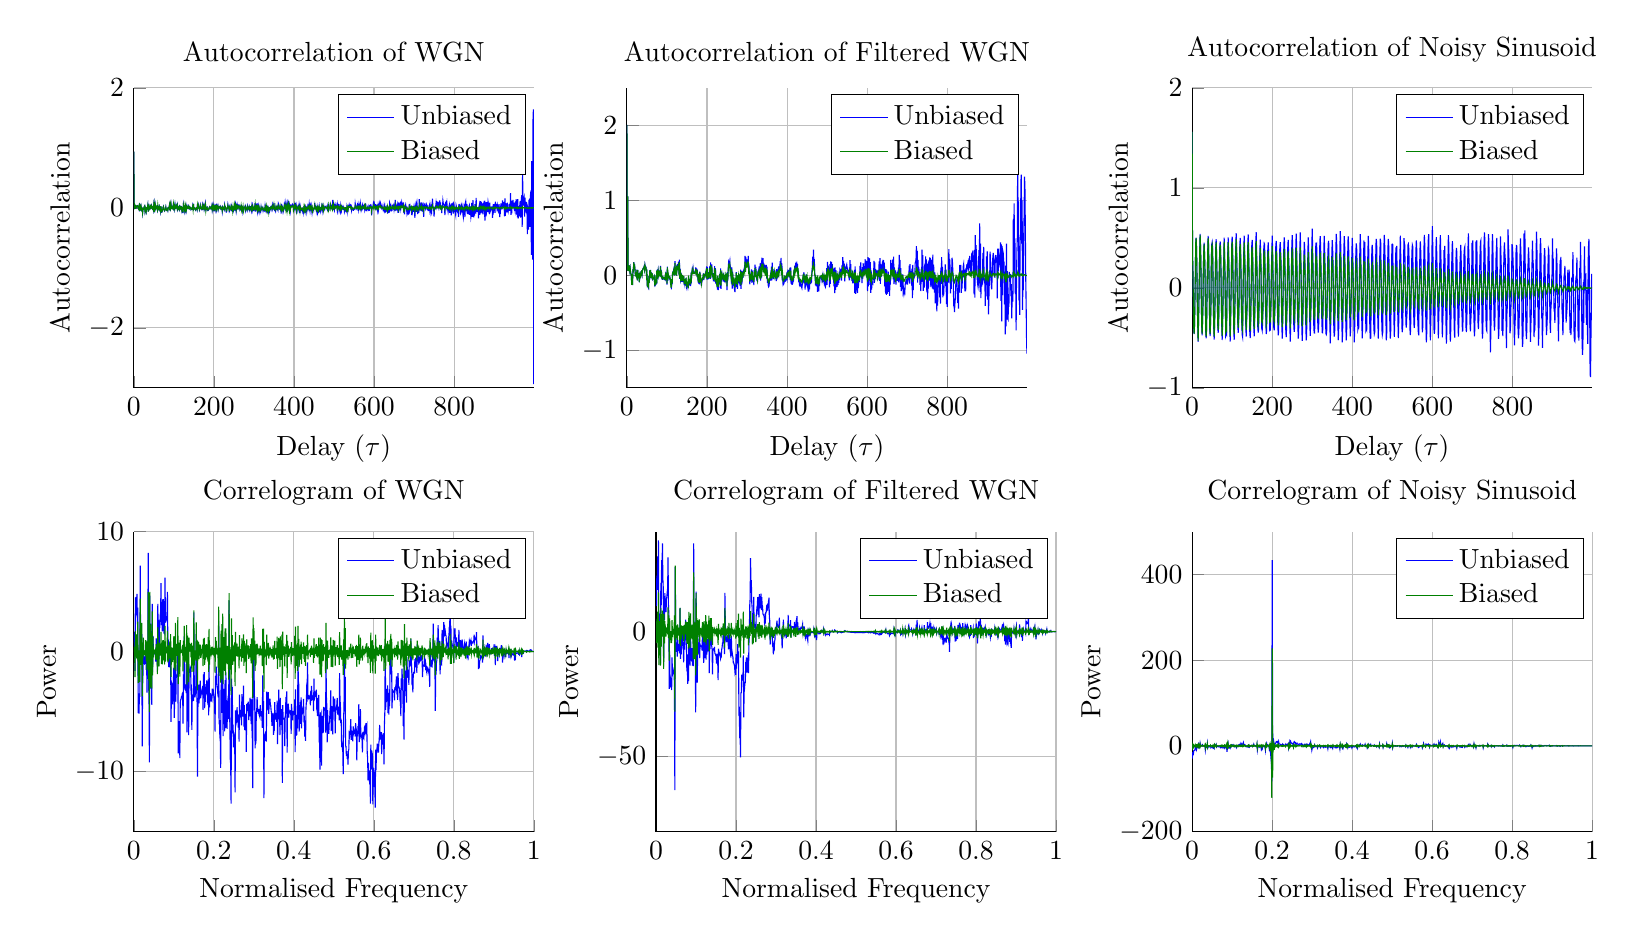
\begin{tikzpicture}

\begin{axis}[%
width=2in,
height=1.5in,
scale only axis,
xmin=0,
xmax=999,
xlabel={Delay ($\tau$)},
xmajorgrids,
ymin=-1.5,
ymax=2.5,
ylabel={Autocorrelation},
ymajorgrids,
name=plot3,
title={Autocorrelation of Filtered WGN},
axis x line*=bottom,
axis y line*=left,
legend style={draw=black,fill=white,legend cell align=left}
]
\addplot [color=blue,solid]
  table[row sep=crcr]{-999	-1.04363351459786\\
-998	-0.815393418274118\\
-997	-0.372948894421538\\
-996	-0.0103770255234643\\
-995	0.633423855500881\\
-994	1.18138138479025\\
-993	1.31502581509801\\
-992	0.815896416656528\\
-991	0.50363649253043\\
-990	-0.1953021425073\\
-989	-0.0623208969984734\\
-988	-0.460736844413034\\
-987	0.998697226826023\\
-986	0.422636304299663\\
-985	1.34394266846885\\
-984	1.25064180494122\\
-983	0.471963224087121\\
-982	0.510025065669935\\
-981	-0.525778308578391\\
-980	-0.203080960845305\\
-979	-0.33228967869119\\
-978	0.985319386508805\\
-977	0.581290893416081\\
-976	1.66264522154805\\
-975	0.50085929513947\\
-974	0.307686212046233\\
-973	-0.0524128016839269\\
-972	-0.732405975746396\\
-971	-0.0115030910098649\\
-970	-0.24900991326284\\
-969	0.493081953610079\\
-968	0.226574586899956\\
-967	0.958517276998491\\
-966	-0.00408138856109009\\
-965	0.753669296615314\\
-964	-0.348754301732965\\
-963	-0.205634581251323\\
-962	-0.326251373594918\\
-961	-0.574526521226671\\
-960	-0.117044334448687\\
-959	-0.276548538634285\\
-958	0.0132107040710342\\
-957	0.0130315032406713\\
-956	-0.0629114071239153\\
-955	0.0450849996345127\\
-954	-0.420282775980449\\
-953	-0.296492803302761\\
-952	-0.586472068895221\\
-951	-0.572449948068382\\
-950	0.057994671830281\\
-949	-0.589511655379882\\
-948	0.422506353218865\\
-947	-0.679105865398074\\
-946	0.13157833960864\\
-945	-0.785058994076771\\
-944	-0.095677851557563\\
-943	-0.3854161812548\\
-942	0.183950967371892\\
-941	0.137404060102939\\
-940	0.292227883752924\\
-939	0.31889582779064\\
-938	-0.262435176262816\\
-937	0.392937255991479\\
-936	-0.614163234633886\\
-935	0.412225226956488\\
-934	-0.339027290280635\\
-933	0.440815022040499\\
-932	0.102191742856405\\
-931	0.257516590021732\\
-930	0.201580682354975\\
-929	0.249374271159448\\
-928	0.357681880094559\\
-927	-0.0413467081156917\\
-926	0.355141967192458\\
-925	-0.307484370266039\\
-924	0.211177920410408\\
-923	0.172205980952393\\
-922	0.261217689458267\\
-921	0.263490775310009\\
-920	0.22390353455266\\
-919	-0.0327427805797715\\
-918	0.146858178152754\\
-917	0.0079437941785853\\
-916	0.212473584610194\\
-915	0.30039436898326\\
-914	0.251897835431449\\
-913	0.15975861323346\\
-912	-0.0449466316445\\
-911	-0.185500590871252\\
-910	-0.125240385695526\\
-909	0.0456877622607144\\
-908	0.177983490036617\\
-907	0.317156630209034\\
-906	-0.0371063312242737\\
-905	-0.092319610455751\\
-904	-0.307961396721437\\
-903	-0.518773409531226\\
-902	-0.0171870496984345\\
-901	-0.324642296503618\\
-900	0.321383389843046\\
-899	-0.1192067080648\\
-898	0.254574416414328\\
-897	-0.279329981886411\\
-896	-0.0256723603242004\\
-895	-0.405839921390248\\
-894	-0.0713724712295286\\
-893	-0.0813020517777816\\
-892	-0.0241487171389569\\
-891	0.381225012972074\\
-890	-0.0658432971270982\\
-889	0.300655315995305\\
-888	-0.121576186865806\\
-887	-0.0444570191510686\\
-886	-0.149990101624881\\
-885	0.0137040348258051\\
-884	-0.303406686864369\\
-883	0.424617330212631\\
-882	-0.219304594336568\\
-881	0.693825505716365\\
-880	0.0205901001278357\\
-879	0.335322280441673\\
-878	-0.102553062357567\\
-877	-0.152332835562867\\
-876	-0.117086699383064\\
-875	-0.0569560046778872\\
-874	0.170256267500391\\
-873	0.23131034764546\\
-872	0.402118150028732\\
-871	0.0331217112508355\\
-870	0.536646027242848\\
-869	-0.295635425135905\\
-868	0.341406904761206\\
-867	-0.254773314069943\\
-866	0.143287555260027\\
-865	-0.00147375030623251\\
-864	0.33127313042529\\
-863	0.249837696651866\\
-862	0.294584376495875\\
-861	0.283434931967355\\
-860	0.00624673992309011\\
-859	0.183634006352344\\
-858	0.0494383351678206\\
-857	0.172647903677639\\
-856	0.258491307169996\\
-855	0.0955983638793474\\
-854	0.226542554870719\\
-853	0.0833989317349563\\
-852	0.100222213414149\\
-851	0.145531991221578\\
-850	0.109239087194665\\
-849	0.14840599310295\\
-848	0.0432763585593717\\
-847	0.101466582559405\\
-846	-0.211559887963582\\
-845	-0.0120646809861329\\
-844	-0.214318803056287\\
-843	0.0772259974317009\\
-842	0.0437693054274404\\
-841	0.152671739260591\\
-840	0.124608241503215\\
-839	0.00948851911921479\\
-838	0.0252171040317903\\
-837	-0.177454846203651\\
-836	0.033937028718229\\
-835	-0.232262963388992\\
-834	0.14027334323948\\
-833	-0.029622249415874\\
-832	0.0483804289319053\\
-831	0.138105385346666\\
-830	-0.231096164905846\\
-829	-0.0743089172998092\\
-828	-0.444053323752499\\
-827	-0.250146456594666\\
-826	-0.365629542441597\\
-825	-0.187843414031856\\
-824	-0.0673701605432181\\
-823	-0.111242759504802\\
-822	-0.0290010480693421\\
-821	-0.172590382563087\\
-820	-0.318929015615383\\
-819	-0.390499066968244\\
-818	-0.489679813569858\\
-817	-0.353886180149101\\
-816	-0.370035871161104\\
-815	-0.0463527205972571\\
-814	0.0582833610749022\\
-813	0.172497244191376\\
-812	0.234564717677152\\
-811	0.0310669819868522\\
-810	-0.180477684920314\\
-809	-0.0580214063798645\\
-808	-0.240071399826351\\
-807	0.117447497572302\\
-806	0.218417366353082\\
-805	0.076523803352465\\
-804	0.35094394361032\\
-803	-0.0958865754402188\\
-802	-0.0585500562977668\\
-801	-0.078398610115434\\
-800	-0.421101398841462\\
-799	-0.0132609843021174\\
-798	-0.382390283664452\\
-797	0.0749426582208418\\
-796	-0.143254242171506\\
-795	0.147483725739245\\
-794	-0.0180492488533522\\
-793	-0.0149761029714219\\
-792	-0.141020431713003\\
-791	-0.268650201805541\\
-790	-0.146198272820216\\
-789	-0.293765082486601\\
-788	0.113125798836355\\
-787	-0.0878365230152614\\
-786	0.242536756872175\\
-785	-0.114485994621044\\
-784	0.102026277035956\\
-783	-0.375826116090936\\
-782	-0.00367579998958882\\
-781	-0.292333941609832\\
-780	-0.0200398305861199\\
-779	-0.0283385794625464\\
-778	-0.161253387720019\\
-777	-0.0558773354942843\\
-776	-0.402172620434134\\
-775	-0.195589912574743\\
-774	-0.480913956973914\\
-773	-0.121267784905008\\
-772	-0.374135776218247\\
-771	0.00637252874262444\\
-770	-0.374466687436208\\
-769	0.038749117662984\\
-768	-0.228565516514098\\
-767	-0.0333370971798334\\
-766	0.141991074311816\\
-765	-0.187836469650783\\
-764	0.277451334599427\\
-763	-0.174911865409052\\
-762	0.206805602410896\\
-761	-0.134917247970532\\
-760	0.178515038100089\\
-759	-0.157026211917172\\
-758	0.234097828942306\\
-757	-0.0691135266025139\\
-756	0.240268737582321\\
-755	-0.0264369041136323\\
-754	0.200072163991382\\
-753	-0.176287774996041\\
-752	0.155373085425498\\
-751	-0.320162411891588\\
-750	0.133245897228892\\
-749	-0.224059379058487\\
-748	0.213389760397435\\
-747	-0.0380900918181716\\
-746	0.253245739775719\\
-745	-0.0560623352441627\\
-744	0.155570969763806\\
-743	-0.162503597890283\\
-742	-0.0787216909796325\\
-741	-0.0469478111583977\\
-740	-0.206954993393662\\
-739	0.271216704442819\\
-738	-0.0819594193359097\\
-737	0.344242894494683\\
-736	-0.0856256139386184\\
-735	0.0879268839787315\\
-734	-0.210961371219659\\
-733	-0.0177473140889584\\
-732	-0.126477682278954\\
-731	0.0374735012215548\\
-730	0.0370407404103204\\
-729	0.106206182251417\\
-728	0.00864028234365415\\
-727	0.207555669246918\\
-726	-0.0974251583841542\\
-725	0.325628164360817\\
-724	0.0228516263248094\\
-723	0.390098567303832\\
-722	0.209946947187263\\
-721	0.181345268743806\\
-720	0.16695028393122\\
-719	-0.00648665552367264\\
-718	-0.0207021068818253\\
-717	0.00872690397768966\\
-716	0.0204860689190695\\
-715	-0.197550050560712\\
-714	0.139607537083428\\
-713	-0.30163646375727\\
-712	0.0911807976146714\\
-711	-0.136913387449996\\
-710	0.0598423378403371\\
-709	0.0114854893821284\\
-708	-0.0408170777916935\\
-707	0.149209391943998\\
-706	-0.110600816859829\\
-705	0.128136207337175\\
-704	-0.0447001379616759\\
-703	-0.0522841348679916\\
-702	-0.0126829161535802\\
-701	-0.122302168636536\\
-700	-0.0781314611297213\\
-699	-0.0586582579803318\\
-698	-0.0914834919591911\\
-697	-0.0729295699411848\\
-696	-0.092864520283798\\
-695	-0.121392278076231\\
-694	-0.227891970976494\\
-693	-0.210542326741654\\
-692	-0.245116675991139\\
-691	-0.188237043357705\\
-690	-0.216799937506776\\
-689	0.0140796560761454\\
-688	-0.186373222547489\\
-687	-0.0156624059431485\\
-686	-0.00473456597227443\\
-685	-0.208611455267537\\
-684	0.0977567308822029\\
-683	-0.15369249794411\\
-682	0.204866107585294\\
-681	-0.0457028662890265\\
-680	0.274590907540447\\
-679	-0.0935624187146587\\
-678	0.10432796564248\\
-677	-0.0651961322350344\\
-676	-0.0550953145517517\\
-675	-0.0110845679624149\\
-674	-0.0741480737395337\\
-673	0.00283736572255142\\
-672	-0.124405166668704\\
-671	0.0664965165230686\\
-670	-0.0899474481134355\\
-669	0.00904619618192852\\
-668	0.105380538354988\\
-667	-0.117167622017734\\
-666	0.250074807238321\\
-665	-0.0545382332464592\\
-664	0.210141662147127\\
-663	0.0384639283777349\\
-662	0.0925723747814932\\
-661	0.163793917658382\\
-660	0.032381808683531\\
-659	0.206878341296832\\
-658	-0.121830446554498\\
-657	-8.60381649881022e-05\\
-656	-0.271964632195568\\
-655	-0.00506609072092226\\
-654	-0.218637376246984\\
-653	0.0488370933927217\\
-652	-0.165671248784754\\
-651	-0.025702930453761\\
-650	-0.246028779738641\\
-649	0.0655475122921821\\
-648	-0.258496070894086\\
-647	0.0831993038157478\\
-646	-0.241576542423754\\
-645	0.0379512999143089\\
-644	-0.147909197400734\\
-643	0.169895208946157\\
-642	0.0679665594755405\\
-641	0.204473931476011\\
-640	0.148879604444391\\
-639	0.113600288191362\\
-638	0.148179117128455\\
-637	0.0702547036639643\\
-636	0.143433067837113\\
-635	-0.0190608063487476\\
-634	0.15457107025356\\
-633	-0.111771210395885\\
-632	0.228837170618131\\
-631	-0.071743104126098\\
-630	0.185941545882583\\
-629	0.0625693460930249\\
-628	0.0221401040886883\\
-627	0.0734860655811582\\
-626	-0.0673862035969657\\
-625	0.030321833114157\\
-624	0.0148781716745851\\
-623	0.0581122958396529\\
-622	0.0677636611538852\\
-621	0.049266310903724\\
-620	-0.0491740462003995\\
-619	0.173371480197314\\
-618	-0.101369027815569\\
-617	0.193152314035515\\
-616	-0.0355538447051377\\
-615	0.00359136627491825\\
-614	-0.109795044103616\\
-613	-0.100003957854625\\
-612	-0.118882216919753\\
-611	-0.188005409665871\\
-610	0.0651930541312509\\
-609	-0.232591394773502\\
-608	0.177607965965497\\
-607	-0.125952332579827\\
-606	0.226188591157512\\
-605	-0.0355798242633409\\
-604	0.230948100458757\\
-603	-0.148209546819232\\
-602	0.243725819168297\\
-601	-0.211174168946405\\
-600	0.189681081389456\\
-599	-0.0262464555726736\\
-598	0.0506105299402483\\
-597	0.194886111419383\\
-596	0.0435117761796245\\
-595	0.215822635178714\\
-594	0.0398136471574751\\
-593	0.0878534833610025\\
-592	0.0556882664943471\\
-591	0.0289924480184822\\
-590	0.163380128558339\\
-589	-0.0443773849659172\\
-588	0.108322830511996\\
-587	-0.104655697315082\\
-586	0.0731928479852909\\
-585	-0.0281463704386725\\
-584	0.172214594530663\\
-583	-0.0174309930635532\\
-582	0.126792345416806\\
-581	-0.0886010596602731\\
-580	-0.032008082296915\\
-579	-0.0283116362222452\\
-578	-0.168913808401335\\
-577	-0.0207419872232183\\
-576	-0.232285906769134\\
-575	-0.0821976997359977\\
-574	-0.171605136450106\\
-573	-0.134921041093445\\
-572	-0.015649557583459\\
-571	-0.246743209832358\\
-570	0.118842037607456\\
-569	-0.234531534224594\\
-568	0.0731062307869774\\
-567	-0.103291804073402\\
-566	-0.0470447722605344\\
-565	0.0172934754464709\\
-564	-0.106255587636175\\
-563	0.0279199426013876\\
-562	-0.0713382939923114\\
-561	0.00774918754642565\\
-560	0.00419334899963453\\
-559	0.150889270078587\\
-558	-0.0310635551654649\\
-557	0.204680402951894\\
-556	-0.0671215253862196\\
-555	0.0726454557985221\\
-554	-0.00617432910267686\\
-553	0.0307176278416534\\
-552	0.0520715671115544\\
-551	0.0947721568429137\\
-550	0.0936890069886494\\
-549	0.144627469641633\\
-548	0.127669914488629\\
-547	0.094894396893292\\
-546	0.039238881837479\\
-545	0.116280187207565\\
-544	-0.0783404716858793\\
-543	0.155265918350937\\
-542	0.0275090814999468\\
-541	0.192993379171168\\
-540	0.132375803666385\\
-539	0.243682212652897\\
-538	0.0242780100519294\\
-537	0.133109040167858\\
-536	-0.0706475678332248\\
-535	0.0883980458062734\\
-534	-0.00742920311421823\\
-533	0.0470888301811684\\
-532	0.0660012241868136\\
-531	-0.0636814869732107\\
-530	0.0502705871189139\\
-529	-0.100183221263006\\
-528	0.0035955406519815\\
-527	-0.129881440332815\\
-526	-0.0279191087412514\\
-525	-0.152248751501673\\
-524	0.0134654277334169\\
-523	-0.157377144267124\\
-522	0.0714532677784389\\
-521	-0.191554709460392\\
-520	0.105556347326613\\
-519	-0.238125986381746\\
-518	0.100457152242553\\
-517	-0.146127420049394\\
-516	0.00670332097091019\\
-515	0.0492814353566478\\
-514	-0.0061836006202535\\
-513	0.150320374889297\\
-512	0.0694512038880981\\
-511	0.176100397479238\\
-510	0.0471274099684376\\
-509	0.186669921360365\\
-508	-0.112304020208373\\
-507	0.148903114847071\\
-506	-0.16041310530124\\
-505	0.107584575355066\\
-504	0.0405497923755594\\
-503	0.129635083685404\\
-502	0.0422386447405541\\
-501	0.179422271239003\\
-500	-0.127234847436161\\
-499	0.0966428207434955\\
-498	-0.0867029521006854\\
-497	-0.115185498669592\\
-496	-0.056151515511808\\
-495	-0.143885978970001\\
-494	-0.127295880880691\\
-493	-0.0250558658864456\\
-492	-0.0728947600448959\\
-491	-0.0300826228508302\\
-490	0.00163415116640336\\
-489	-0.0889010452957629\\
-488	-0.0174997416213614\\
-487	-0.0680713145499883\\
-486	-0.0353847389491655\\
-485	-0.0126716602442486\\
-484	-0.0245235424952779\\
-483	-0.0292520427707615\\
-482	-0.0509104305956739\\
-481	-0.136204886977032\\
-480	-0.0903926493319941\\
-479	-0.213470393871124\\
-478	-0.178789124219512\\
-477	-0.123477290374779\\
-476	-0.220143919503695\\
-475	-0.0629526679797923\\
-474	-0.0934886825771027\\
-473	-0.145595438888114\\
-472	-0.0752171760732223\\
-471	-0.132342925812069\\
-470	-0.0172877532127258\\
-469	0.0256066714734926\\
-468	0.21640426281275\\
-467	0.120712407427533\\
-466	0.341517043401084\\
-465	0.167672531379741\\
-464	0.244823898291092\\
-463	0.10155791652107\\
-462	0.047508399989672\\
-461	-0.0742979407713487\\
-460	-0.0570849738965563\\
-459	-0.0578257594754937\\
-458	-0.115826520292563\\
-457	-0.0333210584573663\\
-456	-0.187375297574722\\
-455	-0.0967052409045339\\
-454	-0.217607619709352\\
-453	-0.134940335813021\\
-452	-0.172133177769243\\
-451	-0.131042341341243\\
-450	-0.0283511531102268\\
-449	-0.0913281903057196\\
-448	0.0142053686157023\\
-447	-0.149339303380931\\
-446	-0.0633782297487008\\
-445	-0.191115153412443\\
-444	-0.0176901680547446\\
-443	-0.107111469237644\\
-442	0.0429177541482039\\
-441	-0.0293783187094339\\
-440	-0.0170237647131021\\
-439	-0.0921448344607363\\
-438	-0.11886108410245\\
-437	-0.168382219300048\\
-436	-0.150510107770763\\
-435	-0.138615341771446\\
-434	-0.10661100697887\\
-433	-0.12589942294672\\
-432	-0.108074865242562\\
-431	-0.123677800333416\\
-430	-0.0642499109046386\\
-429	-0.0706556124967429\\
-428	0.0638788390605739\\
-427	0.0126450091327192\\
-426	0.153590076265782\\
-425	0.120465031292617\\
-424	0.165845025405849\\
-423	0.154135470411936\\
-422	0.10759339469779\\
-421	0.13118146418264\\
-420	0.0642091599352602\\
-419	0.125890440525358\\
-418	0.0246690048477848\\
-417	0.0654600258676778\\
-416	-0.0564632835535846\\
-415	-0.0435797302440827\\
-414	-0.107663760829703\\
-413	-0.118745150866733\\
-412	-0.118902404796852\\
-411	-0.013239148280661\\
-410	-0.112115302963194\\
-409	0.107400818164292\\
-408	-0.0646727661451931\\
-407	0.103365831244846\\
-406	-0.0259997798803164\\
-405	0.0697912034263317\\
-404	0.0131424735486226\\
-403	0.0383083883469368\\
-402	0.00880008940820691\\
-401	0.0323302064190248\\
-400	-0.0381255330871025\\
-399	-0.00432061429014373\\
-398	-0.0534096481340085\\
-397	-0.064326403355663\\
-396	-0.0379032784611924\\
-395	-0.0604426605046968\\
-394	-0.036054627622287\\
-393	-0.0734737080474841\\
-392	-0.111534041969672\\
-391	-0.118891974961638\\
-390	-0.127390861041465\\
-389	-0.00158308833206266\\
-388	-0.0648594139006499\\
-387	0.160826874425125\\
-386	0.00647014323847761\\
-385	0.231547805976654\\
-384	0.0971626283293954\\
-383	0.190927932834994\\
-382	0.123140259012826\\
-381	0.102238882360649\\
-380	0.0389494338830141\\
-379	0.12061822174384\\
-378	-0.0275679094277413\\
-377	0.0646579639192797\\
-376	0.0410342723513924\\
-375	-0.0532203121776232\\
-374	0.0826813800884705\\
-373	-0.0763447498504959\\
-372	0.00258614282820339\\
-371	-0.0266253962093189\\
-370	-0.0105251643719949\\
-369	0.0681095622277292\\
-368	-0.00781540909134312\\
-367	0.060030049936706\\
-366	-0.0509930966273133\\
-365	0.0874727129140728\\
-364	-0.036577316270435\\
-363	0.170687188426994\\
-362	-0.0667969942512456\\
-361	0.115654343536955\\
-360	-0.069303282763808\\
-359	0.0177102297398312\\
-358	-0.015350256527936\\
-357	-0.064247947876866\\
-356	-0.0696154584440945\\
-355	-0.13969120741591\\
-354	-0.15204287107578\\
-353	-0.135022697029114\\
-352	-0.0727257180939212\\
-351	-0.0798738899972572\\
-350	0.115908763325047\\
-349	-0.0445151829179148\\
-348	0.140788513419813\\
-347	-0.0024876413581307\\
-346	0.106020902364141\\
-345	0.0593171179784411\\
-344	0.141388397979843\\
-343	0.0392165041205666\\
-342	0.159651872668595\\
-341	0.0687321432858777\\
-340	0.221240200238566\\
-339	0.219687109941465\\
-338	0.154893265716913\\
-337	0.236539852337069\\
-336	-0.0304188311506921\\
-335	0.167966383672038\\
-334	-0.070445117570371\\
-333	0.160953255902271\\
-332	-0.0404801848410547\\
-331	0.120042137769742\\
-330	0.016182409844642\\
-329	0.0636467151406772\\
-328	0.0282520173730935\\
-327	0.03832603246326\\
-326	-0.0862089700537686\\
-325	-0.0292820789080909\\
-324	-0.0448923940621195\\
-323	-0.0146183721958273\\
-322	0.112084830750243\\
-321	0.0509774553601651\\
-320	0.14220598570714\\
-319	-0.0198259477881476\\
-318	0.0686351195552827\\
-317	-0.130537334645821\\
-316	-0.0154449478465503\\
-315	-0.0824882458604439\\
-314	-0.080461772359904\\
-313	0.0636744456243459\\
-312	-0.0985175595282143\\
-311	0.0800988542483286\\
-310	-0.00196911543268269\\
-309	-0.0722073961978562\\
-308	0.0213606589796812\\
-307	-0.120773953299136\\
-306	-0.0135315568201781\\
-305	0.10100674905661\\
-304	0.0767774668646748\\
-303	0.260661785255525\\
-302	0.151230214653581\\
-301	0.212221497254165\\
-300	0.164263474528681\\
-299	0.158964718803385\\
-298	0.153748681966071\\
-297	0.246668414121229\\
-296	0.0643604451622279\\
-295	0.259847761649349\\
-294	0.0531707636326976\\
-293	0.0909537044457016\\
-292	0.069917998126588\\
-291	0.0660696060715637\\
-290	-0.0332206317883896\\
-289	0.0535083502060757\\
-288	-0.0416229968921667\\
-287	-0.118635386956455\\
-286	0.0601460079488946\\
-285	-0.179659644849917\\
-284	0.077317205369157\\
-283	-0.140559880783286\\
-282	0.0133306433398583\\
-281	-0.0803215709857943\\
-280	-0.0480159008266721\\
-279	-0.00151892940739528\\
-278	-0.107871486889191\\
-277	-0.0164839876419328\\
-276	-0.179333334665256\\
-275	0.00279112899516333\\
-274	-0.157187999417667\\
-273	0.0436488492288501\\
-272	-0.148494176083181\\
-271	-0.0448382709079089\\
-270	-0.221449166380465\\
-269	-0.118367772513843\\
-268	-0.161588230024726\\
-267	-0.125958471390317\\
-266	-0.0387622149445972\\
-265	-0.135809125908628\\
-264	0.0498714918567412\\
-263	-0.177774206914042\\
-262	0.106417075931887\\
-261	-0.111283953049953\\
-260	0.0759331090307746\\
-259	0.101198733213534\\
-258	0.0561375712075762\\
-257	0.190198323853867\\
-256	0.158702636037994\\
-255	0.1511095136889\\
-254	0.172809140795804\\
-253	0.085290472378727\\
-252	-0.0701648570998585\\
-251	0.0418230943048738\\
-250	-0.196117952376165\\
-249	0.0253677380149616\\
-248	-0.0926133747172275\\
-247	-0.0126216271278218\\
-246	-0.0715849705749812\\
-245	-0.0214854727062282\\
-244	-0.0912737302018361\\
-243	0.00469032026600658\\
-242	-0.0815132075866314\\
-241	-0.0105523925549729\\
-240	-0.0411700375148754\\
-239	-0.0259098541537948\\
-238	0.0135285929071386\\
-237	-0.0824425105392952\\
-236	0.0521541478757303\\
-235	-0.178770222622829\\
-234	0.0923338472220928\\
-233	-0.167097685326355\\
-232	0.0217581211784663\\
-231	-0.110792961517042\\
-230	-0.107166417290001\\
-229	-0.0463748961886978\\
-228	-0.197690327305036\\
-227	-0.00580711873661304\\
-226	-0.189387027095872\\
-225	-0.0722344603964152\\
-224	-0.128861137474299\\
-223	-0.063293237646316\\
-222	-0.110567220392975\\
-221	0.0980566579837259\\
-220	-0.0854730391526121\\
-219	0.122133496182033\\
-218	-0.0597220420317676\\
-217	0.0301339755442529\\
-216	-0.0796079903216469\\
-215	0.0201057094653965\\
-214	0.0238467617957407\\
-213	0.00545158010135406\\
-212	0.147431759049758\\
-211	0.0595882391177864\\
-210	0.0364536245933713\\
-209	0.171778553948424\\
-208	-0.0464304595278989\\
-207	0.11967158738872\\
-206	-0.0281805750605865\\
-205	0.0319724419094905\\
-204	-0.0449509351578904\\
-203	0.0435120542819007\\
-202	-0.0547011488250916\\
-201	0.112009185426442\\
-200	-0.0578887337452099\\
-199	0.118634361361266\\
-198	-0.0323338747407007\\
-197	0.0461047794766446\\
-196	0.0234936763588192\\
-195	-0.0024893389411989\\
-194	-0.0066373103310587\\
-193	0.0045798650805042\\
-192	-0.0641853224242818\\
-191	0.0269401134670081\\
-190	-0.031028104614798\\
-189	-0.0360675267936719\\
-188	-0.0672392408780297\\
-187	-0.0832885859503791\\
-186	-0.138491927353381\\
-185	-0.0755711411492776\\
-184	-0.0338089362921981\\
-183	-0.103437554271849\\
-182	0.0481611754166706\\
-181	-0.120468818504238\\
-180	0.0151525985588763\\
-179	-0.11124521064539\\
-178	0.019722165199779\\
-177	-0.0232308897563331\\
-176	0.0418255805108938\\
-175	0.0203178661061408\\
-174	0.0938971999915839\\
-173	0.00292757335583014\\
-172	0.105077163303892\\
-171	0.0471057252447578\\
-170	0.0528566810805744\\
-169	0.0285889307866693\\
-168	0.0294752468004741\\
-167	0.0319765622127797\\
-166	0.0290663616135366\\
-165	0.0939739411313917\\
-164	0.0544023059418741\\
-163	0.0765088286581258\\
-162	0.0364836653103949\\
-161	-0.0552602958102783\\
-160	-0.0248333235644841\\
-159	-0.143430778485294\\
-158	-0.0718595856711487\\
-157	-0.0823257068423137\\
-156	-0.103059728085714\\
-155	-0.0650022689935252\\
-154	-0.13389524081638\\
-153	-0.0771235295366499\\
-152	-0.147067034724923\\
-151	-0.113606520323097\\
-150	-0.108550013120893\\
-149	-0.143835774279284\\
-148	-0.0754631179280989\\
-147	-0.101366977307711\\
-146	-0.0778057254512771\\
-145	-0.115431886144741\\
-144	-0.0552222883709299\\
-143	-0.130217511960649\\
-142	-0.0138501063056188\\
-141	-0.0917683019186468\\
-140	-0.00626147718878808\\
-139	-0.0873389420846605\\
-138	0.00640534486627103\\
-137	-0.0868474479362875\\
-136	-0.00873342995839129\\
-135	-0.033943440857821\\
-134	-0.0581354010230789\\
-133	0.0882067769075481\\
-132	-0.0477665454515415\\
-131	0.208257251421964\\
-130	0.0109958762991628\\
-129	0.183877048612003\\
-128	0.0764900401932535\\
-127	0.14911905717787\\
-126	0.0799082646137254\\
-125	0.143225953097721\\
-124	-0.00306740049477434\\
-123	0.0819796937873217\\
-122	0.042303843006832\\
-121	0.0306020517950055\\
-120	0.188112323654164\\
-119	0.000491797362104517\\
-118	0.120680116955786\\
-117	0.0372868653975865\\
-116	0.0537232473505195\\
-115	0.0247264234742079\\
-114	0.0322244516511055\\
-113	-0.119441428084153\\
-112	-0.0626577241969367\\
-111	-0.18499223864241\\
-110	-0.0576195886550194\\
-109	-0.107217736719664\\
-108	-0.0440292816790989\\
-107	-0.0249740161598221\\
-106	-0.0378075579981581\\
-105	-0.0246501878996028\\
-104	-0.0170044466596933\\
-103	0.0250666246271362\\
-102	-0.0718331673545915\\
-101	0.117028131073322\\
-100	-0.121770699533439\\
-99	0.0359882396672716\\
-98	-0.0584451656621185\\
-97	-0.0585311616163053\\
-96	-0.00826453347747701\\
-95	-0.0568612477038494\\
-94	-0.046609859370896\\
-93	-0.0503741324734114\\
-92	-0.0314453217338547\\
-91	-0.0332994560380093\\
-90	-0.024674500472136\\
-89	-0.0516410677393995\\
-88	-0.0508088195473588\\
-87	-0.0291294527926572\\
-86	0.0661595703189276\\
-85	-0.0022984589175748\\
-84	0.125869901652185\\
-83	-0.024465646307259\\
-82	0.0661878124034748\\
-81	-0.00562567064121403\\
-80	0.0663277297850711\\
-79	0.0134320884262418\\
-78	0.0665838441640203\\
-77	0.02058408591205\\
-76	0.0791526956539579\\
-75	-0.0387718960884523\\
-74	-0.00500454778880552\\
-73	-0.115519466188512\\
-72	-0.113623660517647\\
-71	-0.126208744628982\\
-70	-0.0586826610126015\\
-69	-0.0932039257278569\\
-68	-0.0218700405570183\\
-67	-0.0409339626178173\\
-66	-0.039348645061776\\
-65	-0.0481170765091857\\
-64	-0.00958346909664462\\
-63	-0.0379121192130143\\
-62	-0.0179159292304408\\
-61	0.0400557428651967\\
-60	-0.0352338151067965\\
-59	0.0735049343983383\\
-58	-0.0319636532207356\\
-57	0.065834615365273\\
-56	-0.10111194965723\\
-55	-0.00932092777047381\\
-54	-0.167335306191132\\
-53	-0.154605849592684\\
-52	-0.107908239614522\\
-51	-0.158593405730717\\
-50	0.0198795846641712\\
-49	-0.00669527020813078\\
-48	0.100853524307399\\
-47	0.113375514245935\\
-46	0.10260692679183\\
-45	0.137314550993774\\
-44	0.0803584517200142\\
-43	0.120449254235359\\
-42	0.103115446368568\\
-41	0.0977726203009288\\
-40	0.0894314602829086\\
-39	0.0702031737770385\\
-38	0.0200883735018632\\
-37	0.0674375821194236\\
-36	-0.00594482382568309\\
-35	0.0533452998150266\\
-34	-0.0186781858071727\\
-33	-0.0305556730616651\\
-32	-0.00447875522991109\\
-31	-0.0916551204950295\\
-30	0.0280178276826789\\
-29	-0.027686208994281\\
-28	-0.0308236488308933\\
-27	0.0721394981482458\\
-26	-0.0665723451240716\\
-25	0.0757438182345833\\
-24	-0.0225229856209991\\
-23	-0.0107877327601332\\
-22	0.0225830790277231\\
-21	0.012250207050634\\
-20	0.0862469520584132\\
-19	0.139093627995982\\
-18	0.138059157858124\\
-17	0.174969623639052\\
-16	0.0419740612965344\\
-15	0.0812454923263921\\
-14	-0.129276662658293\\
-13	0.00277898977593677\\
-12	-0.126548363012727\\
-11	0.0123613463482388\\
-10	0.015055381201447\\
-9	0.0463455973248565\\
-8	0.0983231304904412\\
-7	0.0671684330870433\\
-6	0.13261775947866\\
-5	0.0588308503002559\\
-4	0.134854102151819\\
-3	0.0611154265071904\\
-2	1.05481719408915\\
-1	0.0650618432594144\\
0	2.00756555636676\\
1	0.0650618432594143\\
2	1.05481719408915\\
3	0.0611154265071904\\
4	0.134854102151819\\
5	0.0588308503002559\\
6	0.13261775947866\\
7	0.0671684330870433\\
8	0.0983231304904412\\
9	0.0463455973248565\\
10	0.015055381201447\\
11	0.0123613463482388\\
12	-0.126548363012727\\
13	0.00277898977593676\\
14	-0.129276662658293\\
15	0.0812454923263921\\
16	0.0419740612965344\\
17	0.174969623639052\\
18	0.138059157858124\\
19	0.139093627995982\\
20	0.0862469520584132\\
21	0.012250207050634\\
22	0.0225830790277231\\
23	-0.0107877327601332\\
24	-0.0225229856209991\\
25	0.0757438182345833\\
26	-0.0665723451240715\\
27	0.0721394981482458\\
28	-0.0308236488308933\\
29	-0.027686208994281\\
30	0.0280178276826789\\
31	-0.0916551204950295\\
32	-0.00447875522991109\\
33	-0.0305556730616651\\
34	-0.0186781858071727\\
35	0.0533452998150266\\
36	-0.00594482382568306\\
37	0.0674375821194236\\
38	0.0200883735018632\\
39	0.0702031737770385\\
40	0.0894314602829086\\
41	0.0977726203009289\\
42	0.103115446368568\\
43	0.120449254235359\\
44	0.0803584517200142\\
45	0.137314550993774\\
46	0.10260692679183\\
47	0.113375514245935\\
48	0.100853524307399\\
49	-0.0066952702081308\\
50	0.0198795846641712\\
51	-0.158593405730717\\
52	-0.107908239614522\\
53	-0.154605849592684\\
54	-0.167335306191132\\
55	-0.00932092777047379\\
56	-0.10111194965723\\
57	0.065834615365273\\
58	-0.0319636532207355\\
59	0.0735049343983383\\
60	-0.0352338151067964\\
61	0.0400557428651967\\
62	-0.0179159292304408\\
63	-0.0379121192130143\\
64	-0.00958346909664462\\
65	-0.0481170765091857\\
66	-0.039348645061776\\
67	-0.0409339626178174\\
68	-0.0218700405570183\\
69	-0.0932039257278569\\
70	-0.0586826610126015\\
71	-0.126208744628982\\
72	-0.113623660517647\\
73	-0.115519466188512\\
74	-0.00500454778880554\\
75	-0.0387718960884523\\
76	0.0791526956539579\\
77	0.02058408591205\\
78	0.0665838441640203\\
79	0.0134320884262418\\
80	0.0663277297850711\\
81	-0.00562567064121403\\
82	0.0661878124034748\\
83	-0.024465646307259\\
84	0.125869901652185\\
85	-0.00229845891757478\\
86	0.0661595703189277\\
87	-0.0291294527926572\\
88	-0.0508088195473588\\
89	-0.0516410677393995\\
90	-0.024674500472136\\
91	-0.0332994560380093\\
92	-0.0314453217338547\\
93	-0.0503741324734114\\
94	-0.046609859370896\\
95	-0.0568612477038494\\
96	-0.00826453347747701\\
97	-0.0585311616163053\\
98	-0.0584451656621185\\
99	0.0359882396672716\\
100	-0.121770699533439\\
101	0.117028131073322\\
102	-0.0718331673545915\\
103	0.0250666246271362\\
104	-0.0170044466596934\\
105	-0.0246501878996028\\
106	-0.0378075579981581\\
107	-0.0249740161598221\\
108	-0.0440292816790989\\
109	-0.107217736719664\\
110	-0.0576195886550194\\
111	-0.18499223864241\\
112	-0.0626577241969367\\
113	-0.119441428084153\\
114	0.0322244516511055\\
115	0.0247264234742079\\
116	0.0537232473505195\\
117	0.0372868653975865\\
118	0.120680116955786\\
119	0.000491797362104533\\
120	0.188112323654164\\
121	0.0306020517950055\\
122	0.042303843006832\\
123	0.0819796937873216\\
124	-0.00306740049477436\\
125	0.143225953097721\\
126	0.0799082646137254\\
127	0.14911905717787\\
128	0.0764900401932535\\
129	0.183877048612003\\
130	0.0109958762991628\\
131	0.208257251421964\\
132	-0.0477665454515415\\
133	0.0882067769075481\\
134	-0.0581354010230789\\
135	-0.0339434408578209\\
136	-0.00873342995839129\\
137	-0.0868474479362874\\
138	0.00640534486627101\\
139	-0.0873389420846605\\
140	-0.00626147718878808\\
141	-0.0917683019186468\\
142	-0.0138501063056188\\
143	-0.130217511960649\\
144	-0.0552222883709299\\
145	-0.115431886144741\\
146	-0.0778057254512772\\
147	-0.101366977307711\\
148	-0.0754631179280989\\
149	-0.143835774279284\\
150	-0.108550013120893\\
151	-0.113606520323097\\
152	-0.147067034724923\\
153	-0.0771235295366499\\
154	-0.13389524081638\\
155	-0.0650022689935252\\
156	-0.103059728085714\\
157	-0.0823257068423137\\
158	-0.0718595856711487\\
159	-0.143430778485294\\
160	-0.0248333235644841\\
161	-0.0552602958102783\\
162	0.0364836653103949\\
163	0.0765088286581258\\
164	0.0544023059418741\\
165	0.0939739411313917\\
166	0.0290663616135366\\
167	0.0319765622127797\\
168	0.0294752468004741\\
169	0.0285889307866693\\
170	0.0528566810805744\\
171	0.0471057252447578\\
172	0.105077163303892\\
173	0.00292757335583012\\
174	0.0938971999915839\\
175	0.0203178661061408\\
176	0.0418255805108938\\
177	-0.0232308897563332\\
178	0.0197221651997789\\
179	-0.11124521064539\\
180	0.0151525985588763\\
181	-0.120468818504238\\
182	0.0481611754166706\\
183	-0.103437554271849\\
184	-0.0338089362921981\\
185	-0.0755711411492776\\
186	-0.13849192735338\\
187	-0.0832885859503791\\
188	-0.0672392408780297\\
189	-0.0360675267936719\\
190	-0.031028104614798\\
191	0.0269401134670081\\
192	-0.0641853224242818\\
193	0.0045798650805042\\
194	-0.00663731033105864\\
195	-0.00248933894119889\\
196	0.0234936763588192\\
197	0.0461047794766446\\
198	-0.0323338747407007\\
199	0.118634361361266\\
200	-0.0578887337452099\\
201	0.112009185426442\\
202	-0.0547011488250916\\
203	0.0435120542819007\\
204	-0.0449509351578903\\
205	0.0319724419094905\\
206	-0.0281805750605865\\
207	0.11967158738872\\
208	-0.0464304595278989\\
209	0.171778553948424\\
210	0.0364536245933713\\
211	0.0595882391177864\\
212	0.147431759049758\\
213	0.00545158010135405\\
214	0.0238467617957407\\
215	0.0201057094653965\\
216	-0.0796079903216469\\
217	0.0301339755442529\\
218	-0.0597220420317676\\
219	0.122133496182033\\
220	-0.0854730391526121\\
221	0.0980566579837259\\
222	-0.110567220392975\\
223	-0.063293237646316\\
224	-0.128861137474299\\
225	-0.0722344603964152\\
226	-0.189387027095872\\
227	-0.00580711873661305\\
228	-0.197690327305036\\
229	-0.0463748961886978\\
230	-0.107166417290001\\
231	-0.110792961517042\\
232	0.0217581211784663\\
233	-0.167097685326355\\
234	0.0923338472220928\\
235	-0.178770222622829\\
236	0.0521541478757303\\
237	-0.0824425105392952\\
238	0.0135285929071386\\
239	-0.0259098541537949\\
240	-0.0411700375148754\\
241	-0.0105523925549729\\
242	-0.0815132075866314\\
243	0.0046903202660066\\
244	-0.0912737302018361\\
245	-0.0214854727062282\\
246	-0.0715849705749812\\
247	-0.0126216271278218\\
248	-0.0926133747172276\\
249	0.0253677380149617\\
250	-0.196117952376165\\
251	0.0418230943048738\\
252	-0.0701648570998586\\
253	0.085290472378727\\
254	0.172809140795804\\
255	0.1511095136889\\
256	0.158702636037994\\
257	0.190198323853867\\
258	0.0561375712075762\\
259	0.101198733213534\\
260	0.0759331090307746\\
261	-0.111283953049953\\
262	0.106417075931887\\
263	-0.177774206914042\\
264	0.0498714918567412\\
265	-0.135809125908628\\
266	-0.0387622149445972\\
267	-0.125958471390317\\
268	-0.161588230024726\\
269	-0.118367772513843\\
270	-0.221449166380465\\
271	-0.0448382709079088\\
272	-0.148494176083181\\
273	0.0436488492288501\\
274	-0.157187999417667\\
275	0.00279112899516329\\
276	-0.179333334665256\\
277	-0.0164839876419327\\
278	-0.107871486889191\\
279	-0.0015189294073953\\
280	-0.0480159008266721\\
281	-0.0803215709857942\\
282	0.0133306433398582\\
283	-0.140559880783286\\
284	0.077317205369157\\
285	-0.179659644849917\\
286	0.0601460079488946\\
287	-0.118635386956455\\
288	-0.0416229968921667\\
289	0.0535083502060757\\
290	-0.0332206317883895\\
291	0.0660696060715637\\
292	0.069917998126588\\
293	0.0909537044457017\\
294	0.0531707636326976\\
295	0.259847761649349\\
296	0.0643604451622279\\
297	0.246668414121229\\
298	0.153748681966071\\
299	0.158964718803385\\
300	0.164263474528681\\
301	0.212221497254165\\
302	0.151230214653581\\
303	0.260661785255525\\
304	0.0767774668646747\\
305	0.10100674905661\\
306	-0.0135315568201782\\
307	-0.120773953299136\\
308	0.0213606589796812\\
309	-0.0722073961978562\\
310	-0.0019691154326827\\
311	0.0800988542483286\\
312	-0.0985175595282143\\
313	0.0636744456243458\\
314	-0.080461772359904\\
315	-0.0824882458604439\\
316	-0.0154449478465502\\
317	-0.130537334645821\\
318	0.0686351195552827\\
319	-0.0198259477881476\\
320	0.14220598570714\\
321	0.050977455360165\\
322	0.112084830750243\\
323	-0.0146183721958273\\
324	-0.0448923940621194\\
325	-0.0292820789080909\\
326	-0.0862089700537686\\
327	0.0383260324632599\\
328	0.0282520173730935\\
329	0.0636467151406771\\
330	0.016182409844642\\
331	0.120042137769742\\
332	-0.0404801848410548\\
333	0.160953255902271\\
334	-0.0704451175703711\\
335	0.167966383672038\\
336	-0.0304188311506921\\
337	0.236539852337069\\
338	0.154893265716913\\
339	0.219687109941465\\
340	0.221240200238566\\
341	0.0687321432858777\\
342	0.159651872668595\\
343	0.0392165041205667\\
344	0.141388397979843\\
345	0.0593171179784412\\
346	0.106020902364141\\
347	-0.00248764135813072\\
348	0.140788513419813\\
349	-0.0445151829179148\\
350	0.115908763325047\\
351	-0.0798738899972572\\
352	-0.0727257180939212\\
353	-0.135022697029114\\
354	-0.15204287107578\\
355	-0.13969120741591\\
356	-0.0696154584440945\\
357	-0.064247947876866\\
358	-0.015350256527936\\
359	0.0177102297398312\\
360	-0.069303282763808\\
361	0.115654343536955\\
362	-0.0667969942512456\\
363	0.170687188426994\\
364	-0.036577316270435\\
365	0.0874727129140728\\
366	-0.0509930966273133\\
367	0.060030049936706\\
368	-0.0078154090913431\\
369	0.0681095622277292\\
370	-0.0105251643719949\\
371	-0.0266253962093189\\
372	0.00258614282820343\\
373	-0.0763447498504959\\
374	0.0826813800884704\\
375	-0.0532203121776232\\
376	0.0410342723513925\\
377	0.0646579639192798\\
378	-0.0275679094277413\\
379	0.12061822174384\\
380	0.0389494338830141\\
381	0.102238882360649\\
382	0.123140259012826\\
383	0.190927932834994\\
384	0.0971626283293954\\
385	0.231547805976654\\
386	0.00647014323847754\\
387	0.160826874425125\\
388	-0.0648594139006499\\
389	-0.00158308833206267\\
390	-0.127390861041465\\
391	-0.118891974961638\\
392	-0.111534041969672\\
393	-0.0734737080474841\\
394	-0.036054627622287\\
395	-0.0604426605046968\\
396	-0.0379032784611924\\
397	-0.064326403355663\\
398	-0.0534096481340085\\
399	-0.00432061429014373\\
400	-0.0381255330871025\\
401	0.0323302064190248\\
402	0.00880008940820694\\
403	0.0383083883469368\\
404	0.0131424735486226\\
405	0.0697912034263317\\
406	-0.0259997798803164\\
407	0.103365831244846\\
408	-0.064672766145193\\
409	0.107400818164292\\
410	-0.112115302963194\\
411	-0.0132391482806611\\
412	-0.118902404796852\\
413	-0.118745150866733\\
414	-0.107663760829703\\
415	-0.0435797302440827\\
416	-0.0564632835535846\\
417	0.0654600258676778\\
418	0.0246690048477848\\
419	0.125890440525358\\
420	0.0642091599352602\\
421	0.13118146418264\\
422	0.10759339469779\\
423	0.154135470411936\\
424	0.165845025405849\\
425	0.120465031292617\\
426	0.153590076265782\\
427	0.0126450091327192\\
428	0.0638788390605739\\
429	-0.070655612496743\\
430	-0.0642499109046385\\
431	-0.123677800333416\\
432	-0.108074865242561\\
433	-0.12589942294672\\
434	-0.10661100697887\\
435	-0.138615341771446\\
436	-0.150510107770763\\
437	-0.168382219300048\\
438	-0.11886108410245\\
439	-0.0921448344607363\\
440	-0.0170237647131021\\
441	-0.029378318709434\\
442	0.0429177541482039\\
443	-0.107111469237644\\
444	-0.0176901680547446\\
445	-0.191115153412443\\
446	-0.0633782297487008\\
447	-0.149339303380931\\
448	0.0142053686157023\\
449	-0.0913281903057195\\
450	-0.0283511531102268\\
451	-0.131042341341243\\
452	-0.172133177769243\\
453	-0.134940335813021\\
454	-0.217607619709352\\
455	-0.0967052409045339\\
456	-0.187375297574722\\
457	-0.0333210584573663\\
458	-0.115826520292563\\
459	-0.0578257594754937\\
460	-0.0570849738965563\\
461	-0.0742979407713487\\
462	0.047508399989672\\
463	0.10155791652107\\
464	0.244823898291092\\
465	0.167672531379741\\
466	0.341517043401084\\
467	0.120712407427533\\
468	0.21640426281275\\
469	0.0256066714734926\\
470	-0.0172877532127258\\
471	-0.132342925812069\\
472	-0.0752171760732223\\
473	-0.145595438888114\\
474	-0.0934886825771026\\
475	-0.0629526679797923\\
476	-0.220143919503695\\
477	-0.123477290374779\\
478	-0.178789124219512\\
479	-0.213470393871124\\
480	-0.0903926493319941\\
481	-0.136204886977032\\
482	-0.050910430595674\\
483	-0.0292520427707615\\
484	-0.0245235424952779\\
485	-0.0126716602442486\\
486	-0.0353847389491655\\
487	-0.0680713145499883\\
488	-0.0174997416213614\\
489	-0.0889010452957629\\
490	0.00163415116640338\\
491	-0.0300826228508302\\
492	-0.0728947600448959\\
493	-0.0250558658864456\\
494	-0.127295880880691\\
495	-0.14388597897\\
496	-0.056151515511808\\
497	-0.115185498669592\\
498	-0.0867029521006854\\
499	0.0966428207434955\\
500	-0.127234847436161\\
501	0.179422271239003\\
502	0.0422386447405541\\
503	0.129635083685404\\
504	0.0405497923755595\\
505	0.107584575355066\\
506	-0.16041310530124\\
507	0.148903114847071\\
508	-0.112304020208373\\
509	0.186669921360365\\
510	0.0471274099684375\\
511	0.176100397479238\\
512	0.0694512038880981\\
513	0.150320374889297\\
514	-0.00618360062025335\\
515	0.0492814353566478\\
516	0.00670332097091018\\
517	-0.146127420049394\\
518	0.100457152242553\\
519	-0.238125986381746\\
520	0.105556347326613\\
521	-0.191554709460392\\
522	0.0714532677784389\\
523	-0.157377144267124\\
524	0.0134654277334169\\
525	-0.152248751501673\\
526	-0.0279191087412514\\
527	-0.129881440332815\\
528	0.00359554065198156\\
529	-0.100183221263006\\
530	0.0502705871189139\\
531	-0.0636814869732107\\
532	0.0660012241868136\\
533	0.0470888301811684\\
534	-0.00742920311421822\\
535	0.0883980458062735\\
536	-0.0706475678332249\\
537	0.133109040167858\\
538	0.0242780100519293\\
539	0.243682212652897\\
540	0.132375803666385\\
541	0.192993379171168\\
542	0.0275090814999469\\
543	0.155265918350937\\
544	-0.0783404716858793\\
545	0.116280187207565\\
546	0.039238881837479\\
547	0.094894396893292\\
548	0.127669914488628\\
549	0.144627469641633\\
550	0.0936890069886495\\
551	0.0947721568429137\\
552	0.0520715671115544\\
553	0.0307176278416534\\
554	-0.00617432910267688\\
555	0.0726454557985221\\
556	-0.0671215253862196\\
557	0.204680402951894\\
558	-0.0310635551654649\\
559	0.150889270078587\\
560	0.00419334899963452\\
561	0.0077491875464257\\
562	-0.0713382939923113\\
563	0.0279199426013876\\
564	-0.106255587636175\\
565	0.0172934754464709\\
566	-0.0470447722605344\\
567	-0.103291804073402\\
568	0.0731062307869774\\
569	-0.234531534224594\\
570	0.118842037607457\\
571	-0.246743209832358\\
572	-0.0156495575834591\\
573	-0.134921041093445\\
574	-0.171605136450106\\
575	-0.0821976997359976\\
576	-0.232285906769134\\
577	-0.0207419872232183\\
578	-0.168913808401335\\
579	-0.0283116362222452\\
580	-0.032008082296915\\
581	-0.0886010596602731\\
582	0.126792345416806\\
583	-0.0174309930635532\\
584	0.172214594530663\\
585	-0.0281463704386725\\
586	0.0731928479852908\\
587	-0.104655697315082\\
588	0.108322830511996\\
589	-0.0443773849659172\\
590	0.16338012855834\\
591	0.0289924480184823\\
592	0.0556882664943471\\
593	0.0878534833610025\\
594	0.0398136471574751\\
595	0.215822635178714\\
596	0.0435117761796245\\
597	0.194886111419383\\
598	0.0506105299402482\\
599	-0.0262464555726737\\
600	0.189681081389457\\
601	-0.211174168946405\\
602	0.243725819168297\\
603	-0.148209546819232\\
604	0.230948100458757\\
605	-0.0355798242633409\\
606	0.226188591157512\\
607	-0.125952332579827\\
608	0.177607965965497\\
609	-0.232591394773502\\
610	0.065193054131251\\
611	-0.188005409665871\\
612	-0.118882216919753\\
613	-0.100003957854625\\
614	-0.109795044103616\\
615	0.00359136627491829\\
616	-0.0355538447051377\\
617	0.193152314035515\\
618	-0.101369027815569\\
619	0.173371480197314\\
620	-0.0491740462003995\\
621	0.049266310903724\\
622	0.0677636611538853\\
623	0.0581122958396529\\
624	0.0148781716745851\\
625	0.030321833114157\\
626	-0.0673862035969657\\
627	0.0734860655811582\\
628	0.0221401040886883\\
629	0.062569346093025\\
630	0.185941545882583\\
631	-0.071743104126098\\
632	0.228837170618131\\
633	-0.111771210395885\\
634	0.15457107025356\\
635	-0.0190608063487476\\
636	0.143433067837113\\
637	0.0702547036639643\\
638	0.148179117128455\\
639	0.113600288191362\\
640	0.148879604444391\\
641	0.204473931476011\\
642	0.0679665594755403\\
643	0.169895208946157\\
644	-0.147909197400734\\
645	0.0379512999143088\\
646	-0.241576542423754\\
647	0.0831993038157478\\
648	-0.258496070894086\\
649	0.0655475122921821\\
650	-0.246028779738641\\
651	-0.025702930453761\\
652	-0.165671248784754\\
653	0.0488370933927217\\
654	-0.218637376246984\\
655	-0.00506609072092224\\
656	-0.271964632195568\\
657	-8.60381649880711e-05\\
658	-0.121830446554498\\
659	0.206878341296832\\
660	0.032381808683531\\
661	0.163793917658382\\
662	0.0925723747814932\\
663	0.038463928377735\\
664	0.210141662147127\\
665	-0.0545382332464592\\
666	0.250074807238321\\
667	-0.117167622017734\\
668	0.105380538354988\\
669	0.0090461961819285\\
670	-0.0899474481134355\\
671	0.0664965165230686\\
672	-0.124405166668704\\
673	0.00283736572255144\\
674	-0.0741480737395338\\
675	-0.0110845679624149\\
676	-0.0550953145517517\\
677	-0.0651961322350344\\
678	0.10432796564248\\
679	-0.0935624187146587\\
680	0.274590907540446\\
681	-0.0457028662890264\\
682	0.204866107585295\\
683	-0.15369249794411\\
684	0.0977567308822029\\
685	-0.208611455267537\\
686	-0.00473456597227444\\
687	-0.0156624059431485\\
688	-0.186373222547489\\
689	0.0140796560761454\\
690	-0.216799937506776\\
691	-0.188237043357705\\
692	-0.245116675991139\\
693	-0.210542326741654\\
694	-0.227891970976494\\
695	-0.121392278076231\\
696	-0.0928645202837979\\
697	-0.0729295699411847\\
698	-0.0914834919591911\\
699	-0.0586582579803318\\
700	-0.0781314611297212\\
701	-0.122302168636536\\
702	-0.0126829161535802\\
703	-0.0522841348679916\\
704	-0.0447001379616759\\
705	0.128136207337175\\
706	-0.110600816859829\\
707	0.149209391943998\\
708	-0.0408170777916936\\
709	0.0114854893821284\\
710	0.0598423378403371\\
711	-0.136913387449996\\
712	0.0911807976146714\\
713	-0.30163646375727\\
714	0.139607537083428\\
715	-0.197550050560712\\
716	0.0204860689190695\\
717	0.00872690397768972\\
718	-0.0207021068818253\\
719	-0.00648665552367266\\
720	0.16695028393122\\
721	0.181345268743806\\
722	0.209946947187263\\
723	0.390098567303832\\
724	0.0228516263248093\\
725	0.325628164360817\\
726	-0.0974251583841542\\
727	0.207555669246918\\
728	0.00864028234365415\\
729	0.106206182251417\\
730	0.0370407404103204\\
731	0.0374735012215549\\
732	-0.126477682278954\\
733	-0.0177473140889584\\
734	-0.210961371219659\\
735	0.0879268839787315\\
736	-0.0856256139386184\\
737	0.344242894494683\\
738	-0.0819594193359097\\
739	0.271216704442819\\
740	-0.206954993393662\\
741	-0.0469478111583977\\
742	-0.0787216909796324\\
743	-0.162503597890283\\
744	0.155570969763806\\
745	-0.0560623352441628\\
746	0.253245739775719\\
747	-0.0380900918181716\\
748	0.213389760397435\\
749	-0.224059379058487\\
750	0.133245897228892\\
751	-0.320162411891588\\
752	0.155373085425498\\
753	-0.176287774996041\\
754	0.200072163991382\\
755	-0.0264369041136322\\
756	0.240268737582321\\
757	-0.069113526602514\\
758	0.234097828942306\\
759	-0.157026211917172\\
760	0.178515038100089\\
761	-0.134917247970532\\
762	0.206805602410896\\
763	-0.174911865409052\\
764	0.277451334599427\\
765	-0.187836469650783\\
766	0.141991074311816\\
767	-0.0333370971798334\\
768	-0.228565516514098\\
769	0.038749117662984\\
770	-0.374466687436207\\
771	0.0063725287426244\\
772	-0.374135776218247\\
773	-0.121267784905008\\
774	-0.480913956973914\\
775	-0.195589912574743\\
776	-0.402172620434134\\
777	-0.0558773354942843\\
778	-0.161253387720019\\
779	-0.0283385794625465\\
780	-0.02003983058612\\
781	-0.292333941609832\\
782	-0.00367579998958882\\
783	-0.375826116090936\\
784	0.102026277035956\\
785	-0.114485994621044\\
786	0.242536756872175\\
787	-0.0878365230152614\\
788	0.113125798836355\\
789	-0.293765082486601\\
790	-0.146198272820216\\
791	-0.268650201805541\\
792	-0.141020431713003\\
793	-0.0149761029714219\\
794	-0.0180492488533521\\
795	0.147483725739245\\
796	-0.143254242171506\\
797	0.0749426582208419\\
798	-0.382390283664452\\
799	-0.0132609843021174\\
800	-0.421101398841462\\
801	-0.078398610115434\\
802	-0.0585500562977666\\
803	-0.0958865754402188\\
804	0.35094394361032\\
805	0.0765238033524652\\
806	0.218417366353082\\
807	0.117447497572302\\
808	-0.240071399826351\\
809	-0.0580214063798645\\
810	-0.180477684920314\\
811	0.0310669819868521\\
812	0.234564717677152\\
813	0.172497244191376\\
814	0.0582833610749021\\
815	-0.0463527205972571\\
816	-0.370035871161104\\
817	-0.353886180149101\\
818	-0.489679813569858\\
819	-0.390499066968244\\
820	-0.318929015615383\\
821	-0.172590382563087\\
822	-0.0290010480693422\\
823	-0.111242759504802\\
824	-0.067370160543218\\
825	-0.187843414031856\\
826	-0.365629542441597\\
827	-0.250146456594666\\
828	-0.444053323752499\\
829	-0.0743089172998093\\
830	-0.231096164905846\\
831	0.138105385346665\\
832	0.0483804289319053\\
833	-0.0296222494158741\\
834	0.14027334323948\\
835	-0.232262963388992\\
836	0.0339370287182291\\
837	-0.177454846203651\\
838	0.0252171040317903\\
839	0.00948851911921471\\
840	0.124608241503215\\
841	0.152671739260591\\
842	0.0437693054274404\\
843	0.077225997431701\\
844	-0.214318803056287\\
845	-0.0120646809861328\\
846	-0.211559887963582\\
847	0.101466582559405\\
848	0.0432763585593716\\
849	0.14840599310295\\
850	0.109239087194665\\
851	0.145531991221578\\
852	0.100222213414149\\
853	0.0833989317349563\\
854	0.226542554870719\\
855	0.0955983638793474\\
856	0.258491307169995\\
857	0.172647903677639\\
858	0.0494383351678205\\
859	0.183634006352344\\
860	0.00624673992309011\\
861	0.283434931967355\\
862	0.294584376495875\\
863	0.249837696651866\\
864	0.33127313042529\\
865	-0.00147375030623256\\
866	0.143287555260027\\
867	-0.254773314069943\\
868	0.341406904761206\\
869	-0.295635425135905\\
870	0.536646027242848\\
871	0.0331217112508355\\
872	0.402118150028732\\
873	0.23131034764546\\
874	0.170256267500391\\
875	-0.056956004677887\\
876	-0.117086699383064\\
877	-0.152332835562867\\
878	-0.102553062357567\\
879	0.335322280441673\\
880	0.0205901001278357\\
881	0.693825505716365\\
882	-0.219304594336568\\
883	0.424617330212631\\
884	-0.303406686864369\\
885	0.0137040348258052\\
886	-0.149990101624881\\
887	-0.0444570191510686\\
888	-0.121576186865806\\
889	0.300655315995306\\
890	-0.0658432971270982\\
891	0.381225012972074\\
892	-0.0241487171389568\\
893	-0.0813020517777817\\
894	-0.0713724712295288\\
895	-0.405839921390248\\
896	-0.0256723603242004\\
897	-0.279329981886411\\
898	0.254574416414328\\
899	-0.119206708064799\\
900	0.321383389843046\\
901	-0.324642296503618\\
902	-0.0171870496984346\\
903	-0.518773409531226\\
904	-0.307961396721437\\
905	-0.0923196104557509\\
906	-0.0371063312242738\\
907	0.317156630209034\\
908	0.177983490036617\\
909	0.0456877622607144\\
910	-0.125240385695526\\
911	-0.185500590871252\\
912	-0.0449466316444999\\
913	0.15975861323346\\
914	0.251897835431449\\
915	0.30039436898326\\
916	0.212473584610194\\
917	0.00794379417858521\\
918	0.146858178152754\\
919	-0.0327427805797718\\
920	0.22390353455266\\
921	0.263490775310009\\
922	0.261217689458267\\
923	0.172205980952392\\
924	0.211177920410407\\
925	-0.307484370266039\\
926	0.355141967192458\\
927	-0.0413467081156922\\
928	0.357681880094559\\
929	0.249374271159448\\
930	0.201580682354975\\
931	0.257516590021732\\
932	0.102191742856406\\
933	0.440815022040499\\
934	-0.339027290280636\\
935	0.412225226956488\\
936	-0.614163234633886\\
937	0.392937255991479\\
938	-0.262435176262816\\
939	0.31889582779064\\
940	0.292227883752924\\
941	0.137404060102939\\
942	0.183950967371892\\
943	-0.3854161812548\\
944	-0.0956778515575628\\
945	-0.785058994076771\\
946	0.13157833960864\\
947	-0.679105865398074\\
948	0.422506353218865\\
949	-0.589511655379882\\
950	0.057994671830281\\
951	-0.572449948068382\\
952	-0.586472068895222\\
953	-0.296492803302761\\
954	-0.420282775980449\\
955	0.0450849996345121\\
956	-0.0629114071239151\\
957	0.013031503240671\\
958	0.0132107040710336\\
959	-0.276548538634284\\
960	-0.117044334448687\\
961	-0.574526521226671\\
962	-0.326251373594919\\
963	-0.205634581251324\\
964	-0.348754301732965\\
965	0.753669296615314\\
966	-0.00408138856108957\\
967	0.958517276998492\\
968	0.226574586899955\\
969	0.49308195361008\\
970	-0.24900991326284\\
971	-0.0115030910098653\\
972	-0.732405975746395\\
973	-0.0524128016839269\\
974	0.307686212046234\\
975	0.50085929513947\\
976	1.66264522154805\\
977	0.581290893416081\\
978	0.985319386508806\\
979	-0.332289678691192\\
980	-0.203080960845304\\
981	-0.525778308578391\\
982	0.510025065669936\\
983	0.471963224087122\\
984	1.25064180494122\\
985	1.34394266846885\\
986	0.422636304299663\\
987	0.998697226826024\\
988	-0.460736844413034\\
989	-0.0623208969984718\\
990	-0.195302142507299\\
991	0.503636492530428\\
992	0.815896416656528\\
993	1.315025815098\\
994	1.18138138479025\\
995	0.63342385550088\\
996	-0.010377025523467\\
997	-0.372948894421544\\
998	-0.815393418274113\\
999	-1.04363351459789\\
};
\addlegendentry{Unbiased};

\addplot [color=black!50!green,solid]
  table[row sep=crcr]{-999	-0.00104363351459786\\
-998	-0.00163078683654824\\
-997	-0.00111884668326461\\
-996	-4.15081020938573e-05\\
-995	0.00316711927750441\\
-994	0.00708828830874151\\
-993	0.00920518070568604\\
-992	0.00652717133325222\\
-991	0.00453272843277387\\
-990	-0.001953021425073\\
-989	-0.000685529866983208\\
-988	-0.00552884213295641\\
-987	0.0129830639487383\\
-986	0.00591690826019528\\
-985	0.0201591400270327\\
-984	0.0200102688790596\\
-983	0.00802337480948106\\
-982	0.00918045118205884\\
-981	-0.00998978786298943\\
-980	-0.00406161921690609\\
-979	-0.00697808325251499\\
-978	0.0216770265031937\\
-977	0.0133696905485699\\
-976	0.0399034853171532\\
-975	0.0125214823784867\\
-974	0.00799984151320207\\
-973	-0.00141514564546603\\
-972	-0.0205073673208991\\
-971	-0.000333589639286082\\
-970	-0.00747029739788519\\
-969	0.0152855405619125\\
-968	0.00725038678079859\\
-967	0.0316310701409502\\
-966	-0.000138767211077063\\
-965	0.026378425381536\\
-964	-0.0125551548623867\\
-963	-0.00760847950629896\\
-962	-0.0123975521966069\\
-961	-0.0224065343278402\\
-960	-0.00468177337794747\\
-959	-0.0113384900840057\\
-958	0.000554849570983438\\
-957	0.000560354639348867\\
-956	-0.00276810191345227\\
-955	0.00202882498355307\\
-954	-0.0193330076951006\\
-953	-0.0139351617552298\\
-952	-0.0281506593069706\\
-951	-0.0280500474553507\\
-950	0.00289973359151405\\
-949	-0.030065094424374\\
-948	0.021970330367381\\
-947	-0.0359926108660979\\
-946	0.00710523033886655\\
-945	-0.0431782446742224\\
-944	-0.00535795968722353\\
-943	-0.0219687223315236\\
-942	0.0106691561075697\\
-941	0.00810683954607341\\
-940	0.0175336730251754\\
-939	0.0194526454952291\\
-938	-0.0162709809282946\\
-937	0.0247550471274632\\
-936	-0.0393064470165687\\
-935	0.0267946397521717\\
-934	-0.0223758011585219\\
-933	0.0295346064767135\\
-932	0.00694903851423556\\
-931	0.0177686447114995\\
-930	0.0141106477648482\\
-929	0.0177055732523208\\
-928	0.0257530953668083\\
-927	-0.0030183096924455\\
-926	0.0262805055722419\\
-925	-0.0230613277699529\\
-924	0.016049521951191\\
-923	0.0132598605333342\\
-922	0.0203749797777448\\
-921	0.0208157712494907\\
-920	0.0179122827642128\\
-919	-0.00265216522696149\\
-918	0.0120423706085258\\
-917	0.00065933491682258\\
-916	0.0178477811072563\\
-915	0.0255335213635771\\
-914	0.0216632138471046\\
-913	0.013898999351311\\
-912	-0.003955303584716\\
-911	-0.0165095525875414\\
-910	-0.0112716347125973\\
-909	0.00415758636572501\\
-908	0.0163744810833688\\
-907	0.0294955666094402\\
-906	-0.00348799513508173\\
-905	-0.00877036299329634\\
-904	-0.0295642940852579\\
-903	-0.0503210207245289\\
-902	-0.00168433087044658\\
-901	-0.0321395873538582\\
-900	0.0321383389843046\\
-899	-0.0120398775145448\\
-898	0.0259665904742615\\
-897	-0.0287709881343003\\
-896	-0.00266992547371684\\
-895	-0.042613191745976\\
-894	-0.00756548195033003\\
-893	-0.00869931954022263\\
-892	-0.00260806145100734\\
-891	0.0415535264139561\\
-890	-0.0072427626839808\\
-889	0.0333727400754789\\
-888	-0.0136165329289703\\
-887	-0.00502364316407075\\
-886	-0.0170988715852365\\
-885	0.00157596400496758\\
-884	-0.0351951756762668\\
-883	0.0496802276348778\\
-882	-0.025877942131715\\
-881	0.0825652351802475\\
-880	0.00247081201534029\\
-879	0.0405739959334424\\
-878	-0.0125114736076231\\
-877	-0.0187369387742326\\
-876	-0.0145187507235\\
-875	-0.0071195005847359\\
-874	0.0214522897050493\\
-873	0.0293764141509734\\
-872	0.0514711232036777\\
-871	0.00427270075135779\\
-870	0.0697639835415703\\
-869	-0.0387282406928035\\
-868	0.0450657114284792\\
-867	-0.0338848507713025\\
-866	0.0192005324048436\\
-865	-0.000198956291341389\\
-864	0.0450531457378394\\
-863	0.0342277644413057\\
-862	0.0406526439564308\\
-861	0.0393974555434624\\
-860	0.000874543589232616\\
-859	0.0258923948956805\\
-858	0.00702024359383053\\
-857	0.0246886502259024\\
-856	0.0372227482324794\\
-855	0.0138617627625054\\
-854	0.033075213011125\\
-853	0.0122596429650386\\
-852	0.014832887585294\\
-851	0.0216842666920151\\
-850	0.0163858630791997\\
-849	0.0224093049585454\\
-848	0.0065780065010245\\
-847	0.0155243871315889\\
-846	-0.0325802227463916\\
-845	-0.00187002555285059\\
-844	-0.0334337332767807\\
-843	0.012124481596777\\
-842	0.00691555025753559\\
-841	0.024274806542434\\
-840	0.0199373186405144\\
-839	0.00152765157819358\\
-838	0.00408517085315003\\
-837	-0.0289251399311951\\
-836	0.00556567270978955\\
-835	-0.0383233889591837\\
-834	0.0232853749777537\\
-833	-0.00494691565245096\\
-832	0.00812791206056009\\
-831	0.0233398101235865\\
-830	-0.0392863480339938\\
-829	-0.0127068248582674\\
-828	-0.0763771716854298\\
-827	-0.0432753369908771\\
-826	-0.0636195403848379\\
-825	-0.0328725974555748\\
-824	-0.0118571482556064\\
-823	-0.01968996843235\\
-822	-0.00516218655634289\\
-821	-0.0308936784787925\\
-820	-0.057407222810769\\
-819	-0.0706803311212522\\
-818	-0.0891217260697142\\
-817	-0.0647611709672855\\
-816	-0.0680866002936431\\
-815	-0.00857525331049257\\
-814	0.0108407051599318\\
-813	0.0322569846637873\\
-812	0.0440981669233047\\
-811	0.00587165959551506\\
-810	-0.0342907601348597\\
-809	-0.0110820886185541\\
-808	-0.0460937087666594\\
-807	0.0226673670314543\\
-806	0.042372969072498\\
-805	0.0149221416537307\\
-804	0.0687850129476227\\
-803	-0.0188896553617231\\
-802	-0.0115929111469578\\
-801	-0.0156013234129714\\
-800	-0.0842202797682925\\
-799	-0.00266545784472559\\
-798	-0.0772428373002194\\
-797	0.0152133596188309\\
-796	-0.0292238654029872\\
-795	0.0302341637765451\\
-794	-0.00371814526379054\\
-793	-0.00310005331508433\\
-792	-0.0293322497963046\\
-791	-0.0561478921773581\\
-790	-0.0307016372922454\\
-789	-0.0619844324046728\\
-788	0.0239826693533072\\
-787	-0.0187091794022507\\
-786	0.0519028659706454\\
-785	-0.0246144888435245\\
-784	0.0220376758397664\\
-783	-0.0815542671917331\\
-782	-0.000801324397730362\\
-781	-0.0640211332125531\\
-780	-0.00440876272894639\\
-779	-0.00626282606122276\\
-778	-0.0357982520738443\\
-777	-0.0124606458152254\\
-776	-0.0900866669772459\\
-775	-0.0440077303293172\\
-774	-0.108686554276105\\
-773	-0.0275277871734368\\
-772	-0.0853029569777603\\
-771	0.001459309082061\\
-770	-0.0861273381103278\\
-769	0.0089510461801493\\
-768	-0.0530271998312707\\
-767	-0.00776754364290118\\
-766	0.033225911388965\\
-765	-0.0441415703679339\\
-764	0.0654785149654647\\
-763	-0.0414541121019453\\
-762	0.0492197333737932\\
-761	-0.0322452222649572\\
-760	0.0428436091440214\\
-759	-0.0378433170720384\\
-758	0.0566516746040381\\
-757	-0.0167945869644109\\
-756	0.0586255719700862\\
-755	-0.00647704150783991\\
-754	0.0492177523418799\\
-753	-0.0435430804240221\\
-752	0.0385325251855235\\
-751	-0.0797204405610054\\
-750	0.0333114743072231\\
-749	-0.0562389041436803\\
-748	0.0537742196201537\\
-747	-0.00963679322999742\\
-746	0.0643244179030325\\
-745	-0.0142958954872615\\
-744	0.0398261682595345\\
-743	-0.0417634246578027\\
-742	-0.0203101962727452\\
-741	-0.012159483090025\\
-740	-0.053808298282352\\
-739	0.0707875598595757\\
-738	-0.0214733678660083\\
-737	0.0905358812521017\\
-736	-0.0226051620797952\\
-735	0.0233006242543638\\
-734	-0.0561157247444293\\
-733	-0.00473853286175189\\
-732	-0.0338960188507596\\
-731	0.0100803718285982\\
-730	0.0100009999107865\\
-729	0.0287818753901339\\
-728	0.00235015679747393\\
-727	0.0566626977044088\\
-726	-0.0266944933972582\\
-725	0.0895477451992247\\
-724	0.00630704886564739\\
-723	0.108057303143162\\
-722	0.0583652513180592\\
-721	0.050595329979522\\
-720	0.0467460795007417\\
-719	-0.00182275020215201\\
-718	-0.00583799414067473\\
-717	0.00246971382568617\\
-716	0.00581804357301573\\
-715	-0.056301764409803\\
-714	0.0399277556058604\\
-713	-0.0865696650983364\\
-712	0.0262600697130254\\
-711	-0.0395679689730489\\
-710	0.0173542779736978\\
-709	0.00334227741019937\\
-708	-0.0119185867151745\\
-707	0.0437183518395913\\
-706	-0.0325166401567898\\
-705	0.0378001811644667\\
-704	-0.0132312408366561\\
-703	-0.0155283880557935\\
-702	-0.00377950901376689\\
-701	-0.0365683484223242\\
-700	-0.0234394383389164\\
-699	-0.0176561356520799\\
-698	-0.0276280145716757\\
-697	-0.022097659692179\\
-696	-0.0282308141662746\\
-695	-0.0370246448132506\\
-694	-0.069734943118807\\
-693	-0.0646364943096877\\
-692	-0.0754959362052708\\
-691	-0.0581652463975308\\
-690	-0.0672079806271004\\
-689	0.00437877303968122\\
-688	-0.0581484454348166\\
-687	-0.00490233306020548\\
-686	-0.00148665371529417\\
-685	-0.0657126084092743\\
-684	0.0308911269587761\\
-683	-0.048720521848283\\
-682	0.0651474222121236\\
-681	-0.0145792143461995\\
-680	0.0878690904129429\\
-679	-0.0300335364074054\\
-678	0.0335936049368786\\
-677	-0.0210583507119161\\
-676	-0.0178508819147676\\
-675	-0.00360248458778485\\
-674	-0.024172272039088\\
-673	0.000927818591274315\\
-672	-0.040804894667335\\
-671	0.0218773539360896\\
-670	-0.0296826578774337\\
-669	0.00299429093621834\\
-668	0.034986338733856\\
-667	-0.0390168181319056\\
-666	0.0835249856175994\\
-665	-0.0182703081375638\\
-664	0.0706075984814347\\
-663	0.0129623438632967\\
-662	0.0312894626761447\\
-661	0.0555261380861914\\
-660	0.0110098149524005\\
-659	0.0705455143822197\\
-658	-0.0416660127216385\\
-657	-2.95110905909191e-05\\
-656	-0.0935558334752753\\
-655	-0.00174780129871818\\
-654	-0.0756485321814566\\
-653	0.0169464714072744\\
-652	-0.0576535945770942\\
-651	-0.0089703227283626\\
-650	-0.0861100729085245\\
-649	0.0230071768145559\\
-648	-0.0909906169547182\\
-647	0.029369354246959\\
-646	-0.0855180960180091\\
-645	0.0134727114695797\\
-644	-0.0526556742746613\\
-643	0.060652589593778\\
-642	0.0243320282922435\\
-641	0.0734061413998881\\
-640	0.0535966575999808\\
-639	0.0410097040370817\\
-638	0.0536408404005007\\
-637	0.025502457430019\\
-636	0.0522096366927093\\
-635	-0.00695719431729289\\
-634	0.0565730117128031\\
-633	-0.0410200342152898\\
-632	0.0842120787874723\\
-631	-0.0264732054225302\\
-630	0.0687983719765557\\
-629	0.0232132274005122\\
-628	0.00823611872099205\\
-627	0.027410302461772\\
-626	-0.0252024401452652\\
-625	0.0113706874178089\\
-624	0.00559419254964401\\
-623	0.0219083355315491\\
-622	0.0256146639161686\\
-621	0.0186719318325114\\
-620	-0.0186861375561518\\
-619	0.0660545339551767\\
-618	-0.0387229686255473\\
-617	0.0739773362756022\\
-616	-0.0136526763667729\\
-615	0.00138267601584353\\
-614	-0.0423808870239957\\
-613	-0.0387015316897398\\
-612	-0.0461263001648643\\
-611	-0.0731341043600238\\
-610	0.0254252911111878\\
-609	-0.0909432353564392\\
-608	0.0696223226584749\\
-607	-0.0494992667038719\\
-606	0.0891183049160596\\
-605	-0.0140540305840197\\
-604	0.0914554477816679\\
-603	-0.058839190087235\\
-602	0.0970028760289821\\
-601	-0.0842584934096157\\
-600	0.0758724325557826\\
-599	-0.0105248286846421\\
-598	0.0203454330359798\\
-597	0.0785391029020115\\
-596	0.0175787575765683\\
-595	0.0874081672473792\\
-594	0.0161643407459349\\
-593	0.035756367727928\\
-592	0.0227208127296936\\
-591	0.0118579112395592\\
-590	0.0669858527089192\\
-589	-0.018239105220992\\
-588	0.0446290061709424\\
-587	-0.043222802991129\\
-586	0.0303018390659104\\
-585	-0.0116807437320491\\
-584	0.0716412713247557\\
-583	-0.00726872410750169\\
-582	0.0529992003842247\\
-581	-0.0371238439976544\\
-580	-0.0134433945647043\\
-579	-0.0119191988495652\\
-578	-0.0712816271453634\\
-577	-0.00877386059542135\\
-576	-0.0984892244701126\\
-575	-0.034934022387799\\
-574	-0.073103788127745\\
-573	-0.0576112845469011\\
-572	-0.00669801064572046\\
-571	-0.105852837018082\\
-570	0.0511020761712063\\
-569	-0.1010830912508\\
-568	0.0315818916999742\\
-567	-0.0447253511637833\\
-566	-0.0204174311610719\\
-565	0.00752266181921485\\
-564	-0.0463274362093723\\
-563	0.0122010149168064\\
-562	-0.0312461727686324\\
-561	0.00340189333288086\\
-560	0.00184507355983919\\
-559	0.0665421681046567\\
-558	-0.0137300913831355\\
-557	0.090673418507689\\
-556	-0.0298019572714815\\
-555	0.0323272278303423\\
-554	-0.00275375077979388\\
-553	0.0137307796452191\\
-552	0.0233280620659764\\
-551	0.0425526984224682\\
-550	0.0421600531448923\\
-549	0.0652269888083765\\
-548	0.0577068013488601\\
-547	0.0429871617926613\\
-546	0.0178144523542155\\
-545	0.0529074851794419\\
-544	-0.035723255088761\\
-543	0.0709565246863782\\
-542	0.0125991593269756\\
-541	0.0885839610395662\\
-540	0.0608928696865369\\
-539	0.112337500032985\\
-538	0.0112164406439914\\
-537	0.0616294855977182\\
-536	-0.0327804714746163\\
-535	0.0411050912999172\\
-534	-0.0034620086512257\\
-533	0.0219904836946057\\
-532	0.0308885729194288\\
-531	-0.0298666173904358\\
-530	0.0236271759458895\\
-529	-0.047186297214876\\
-528	0.00169709518773527\\
-527	-0.0614339212774214\\
-526	-0.0132336575433532\\
-525	-0.0723181569632947\\
-524	0.00640954360110645\\
-523	-0.0750688978154183\\
-522	0.0341546619980938\\
-521	-0.0917547058315279\\
-520	0.0506670467167743\\
-519	-0.11453859944962\\
-518	0.0484203473809105\\
-517	-0.0705795438838574\\
-516	0.00324440734992053\\
-515	0.0239014961479742\\
-514	-0.0030052299014432\\
-513	0.0732060225710876\\
-512	0.0338921874973919\\
-511	0.0861130943673473\\
-510	0.0230924308845344\\
-509	0.0916549313879393\\
-508	-0.0552535779425196\\
-507	0.0734092356196059\\
-506	-0.0792440740188127\\
-505	0.0532543648007577\\
-504	0.0201126970182775\\
-503	0.0644286365916456\\
-502	0.0210348450807959\\
-501	0.0895317133482623\\
-500	-0.0636174237180803\\
-499	0.0484180531924912\\
-498	-0.0435248819545441\\
-497	-0.057938305830805\\
-496	-0.0283003638179512\\
-495	-0.0726624193798503\\
-494	-0.0644117157256297\\
-493	-0.0127033240044279\\
-492	-0.0370305381028071\\
-491	-0.0153120550310726\\
-490	0.000833417094865715\\
-489	-0.0454284341461348\\
-488	-0.00895986771013706\\
-487	-0.034920584364144\\
-486	-0.0181877558198711\\
-485	-0.00652590502578805\\
-484	-0.0126541479275634\\
-483	-0.0151233061124837\\
-482	-0.0263716030485591\\
-481	-0.0706903363410798\\
-480	-0.047004177652637\\
-479	-0.111218075206856\\
-478	-0.0933279228425853\\
-477	-0.0645786228660095\\
-476	-0.115355413819936\\
-475	-0.0330501506893909\\
-474	-0.049175047035556\\
-473	-0.0767287962940363\\
-472	-0.0397146689666614\\
-471	-0.0700094077545847\\
-470	-0.00916250920274466\\
-469	0.0135971425524246\\
-468	0.115127067816383\\
-467	0.0643397131588752\\
-466	0.182370101176179\\
-465	0.0897048042881614\\
-464	0.131225609484025\\
-463	0.0545366011718146\\
-462	0.0255595191944435\\
-461	-0.0400465900757569\\
-460	-0.0308258859041404\\
-459	-0.0312837358762421\\
-458	-0.062777973998569\\
-457	-0.0180933347423499\\
-456	-0.101932161880649\\
-455	-0.052704356292971\\
-454	-0.118813760361306\\
-453	-0.0738123636897223\\
-452	-0.0943289814175452\\
-451	-0.0719422453963423\\
-450	-0.0155931342106247\\
-449	-0.0503218328584515\\
-448	0.00784136347586765\\
-447	-0.0825846347696546\\
-446	-0.0351115392807802\\
-445	-0.106068910143906\\
-444	-0.00983573343843798\\
-443	-0.0596610883653675\\
-442	0.0239481068146978\\
-441	-0.0164224801585736\\
-440	-0.00953330823933719\\
-439	-0.0516932521324731\\
-438	-0.0667999292655769\\
-437	-0.0947991894659272\\
-436	-0.0848877007827104\\
-435	-0.0783176681008672\\
-434	-0.0603418299500407\\
-433	-0.0713849728107903\\
-432	-0.0613865234577749\\
-431	-0.0703726683897137\\
-430	-0.036622449215644\\
-429	-0.0403443547356402\\
-428	0.0365386959426483\\
-427	0.00724559023304808\\
-426	0.0881607037765588\\
-425	0.0692673929932546\\
-424	0.0955267346337692\\
-423	0.0889361664276869\\
-422	0.0621889821353228\\
-421	0.0759540677617483\\
-420	0.0372413127624509\\
-419	0.073142345945233\\
-418	0.0143573608214107\\
-417	0.0381631950808562\\
-416	-0.0329745575952934\\
-415	-0.0254941421927884\\
-414	-0.0630909638462059\\
-413	-0.0697034035587722\\
-412	-0.069914614020549\\
-411	-0.00779785833730936\\
-410	-0.0661480287482847\\
-409	0.0634738835350966\\
-408	-0.0382862775579543\\
-407	0.0612959379281938\\
-406	-0.0154438692489079\\
-405	0.0415257660386674\\
-404	0.00783291423497907\\
-403	0.0228701078431213\\
-402	0.00526245346610773\\
-401	0.0193657936449959\\
-400	-0.0228753198522615\\
-399	-0.00259668918837638\\
-398	-0.0321526081766731\\
-397	-0.0387888212234648\\
-396	-0.0228935801905602\\
-395	-0.0365678096053416\\
-394	-0.0218491043391059\\
-393	-0.0445985407848229\\
-392	-0.0678126975175603\\
-391	-0.0724052127516378\\
-390	-0.0777084252352935\\
-389	-0.000967266970890282\\
-388	-0.0396939613071977\\
-387	0.0985868740226017\\
-386	0.00397266794842525\\
-385	0.142401900675642\\
-384	0.0598521790509075\\
-383	0.117802534559191\\
-382	0.0761006800699264\\
-381	0.063285868181242\\
-380	0.0241486490074688\\
-379	0.0749039157029246\\
-378	-0.0171472396640551\\
-377	0.0402819115217113\\
-376	0.0256053859472689\\
-375	-0.0332626951110145\\
-374	0.0517585439353825\\
-373	-0.047868158156261\\
-372	0.00162409769611173\\
-371	-0.0167473742156616\\
-370	-0.00663085355435677\\
-369	0.0429771337656971\\
-368	-0.00493933854572886\\
-367	0.0379990216099349\\
-366	-0.0323296232617167\\
-365	0.0555451727004362\\
-364	-0.0232631731479967\\
-363	0.108727739027995\\
-362	-0.0426164823322947\\
-361	0.0739031255201141\\
-360	-0.0443541009688371\\
-359	0.0113522572632318\\
-358	-0.00985486469093493\\
-357	-0.0413114304848248\\
-356	-0.0448323552379969\\
-355	-0.0901008287832622\\
-354	-0.0982196947149542\\
-353	-0.0873596849778366\\
-352	-0.0471262653248609\\
-351	-0.0518381546082199\\
-350	0.0753406961612803\\
-349	-0.0289793840795626\\
-348	0.0917941107497181\\
-347	-0.00162442980685935\\
-346	0.0693376701461479\\
-345	0.0388527122758789\\
-344	0.0927507890747769\\
-343	0.0257652432072123\\
-342	0.105050932215936\\
-341	0.0452944824253934\\
-340	0.146018532157453\\
-339	0.145213179671308\\
-338	0.102539341904597\\
-337	0.156825922099477\\
-336	-0.0201981038840595\\
-335	0.111697645141905\\
-334	-0.0469164483018671\\
-333	0.107355821686815\\
-332	-0.0270407634738246\\
-331	0.0803081901679577\\
-330	0.0108422145959101\\
-329	0.0427069458593944\\
-328	0.0189853556747188\\
-327	0.025793419847774\\
-326	-0.05810484581624\\
-325	-0.0197654032629614\\
-324	-0.0303472583859928\\
-323	-0.00989663797657509\\
-322	0.0759935152486648\\
-321	0.0346136921895521\\
-320	0.0967000702808551\\
-319	-0.0135014704437285\\
-318	0.0468091515367028\\
-317	-0.0891569995630958\\
-316	-0.0105643443270404\\
-315	-0.056504448414404\\
-314	-0.0551967758388942\\
-313	0.0437443441439256\\
-312	-0.0677800809554114\\
-311	0.0551881105770984\\
-310	-0.00135868964855106\\
-309	-0.0498953107727186\\
-308	0.0147815760139394\\
-307	-0.0836963496363012\\
-306	-0.00939090043320363\\
-305	0.0701996905943437\\
-304	0.0534371169378136\\
-303	0.181681264323101\\
-302	0.105558689828199\\
-301	0.148342826580661\\
-300	0.114984432170077\\
-299	0.111434267881173\\
-298	0.107931574740182\\
-297	0.173407895127224\\
-296	0.0453097533942084\\
-295	0.183192671962791\\
-294	0.0375385591246845\\
-293	0.0643042690431111\\
-292	0.0495019426736243\\
-291	0.0468433507047387\\
-290	-0.0235866485697566\\
-289	0.0380444369965198\\
-288	-0.0296355737872227\\
-287	-0.0845870308999524\\
-286	0.0429442496755107\\
-285	-0.128456646067691\\
-284	0.0553591190443164\\
-283	-0.100781434521616\\
-282	0.00957140191801823\\
-281	-0.0577512095387861\\
-280	-0.0345714485952039\\
-279	-0.001095148102732\\
-278	-0.0778832135339962\\
-277	-0.0119179230651174\\
-276	-0.129837334297645\\
-275	0.00202356852149342\\
-274	-0.114118487577227\\
-273	0.031732713389374\\
-272	-0.108103760188556\\
-271	-0.0326870994918656\\
-270	-0.161657891457739\\
-269	-0.086526841707619\\
-268	-0.118282584378099\\
-267	-0.0923275595291021\\
-266	-0.0284514657693343\\
-265	-0.0998197075428418\\
-264	0.0367054180065615\\
-263	-0.131019590495649\\
-262	0.0785358020377325\\
-261	-0.0822388413039154\\
-260	0.0561905006827732\\
-259	0.0749882613112286\\
-258	0.0416540778360215\\
-257	0.141317354623423\\
-256	0.118074761212268\\
-255	0.11257658769823\\
-254	0.12891561903367\\
-253	0.0637119828669091\\
-252	-0.0524833131106942\\
-251	0.0313254976343504\\
-250	-0.147088464282124\\
-249	0.0190511712492362\\
-248	-0.0696452577873551\\
-247	-0.00950408522724979\\
-246	-0.0539750678135358\\
-245	-0.0162215318932023\\
-244	-0.0690029400325881\\
-243	0.00355057244136698\\
-242	-0.0617870113506666\\
-241	-0.00800926594922444\\
-240	-0.0312892285113053\\
-239	-0.0197173990110379\\
-238	0.0103087877952396\\
-237	-0.0629036355414822\\
-236	0.0398457689770579\\
-235	-0.136759220306464\\
-234	0.0707277269721231\\
-233	-0.128163924645315\\
-232	0.0167102370650621\\
-231	-0.085199787406605\\
-230	-0.082518141313301\\
-229	-0.035755044961486\\
-228	-0.152616932679488\\
-227	-0.00448890278340188\\
-226	-0.146585558972205\\
-225	-0.0559817068072218\\
-224	-0.0999962426800561\\
-223	-0.0491788456511875\\
-222	-0.0860212974657346\\
-221	0.0763861365693225\\
-220	-0.0666689705390374\\
-219	0.0953862605181676\\
-218	-0.0467026368688422\\
-217	0.02359490285115\\
-216	-0.0624126644121712\\
-215	0.0157829819303362\\
-214	0.0187435547714522\\
-213	0.00429039353976565\\
-212	0.116176226131209\\
-211	0.0470151206639335\\
-210	0.0287983634287633\\
-209	0.135876836173203\\
-208	-0.0367729239460959\\
-207	0.0948995687992547\\
-206	-0.0223753765981057\\
-205	0.025418091318045\\
-204	-0.0357809443856807\\
-203	0.0346791072626749\\
-202	-0.0436515167624231\\
-201	0.089495339155727\\
-200	-0.0463109869961679\\
-199	0.0950261234503737\\
-198	-0.025931767542042\\
-197	0.0370221379197456\\
-196	0.0188889157924907\\
-195	-0.00200391784766511\\
-194	-0.00534967212683331\\
-193	0.00369595111996689\\
-192	-0.0518617405188197\\
-191	0.0217945517948096\\
-190	-0.0251327647379864\\
-189	-0.0292507642296679\\
-188	-0.0545982635929601\\
-187	-0.0677136203776582\\
-186	-0.112732428865652\\
-185	-0.0615904800366612\\
-184	-0.0275880920144337\\
-183	-0.0845084818401004\\
-182	0.0393958414908366\\
-181	-0.0986639623549706\\
-180	0.0124251308182786\\
-179	-0.0913323179398654\\
-178	0.0162116197942183\\
-177	-0.0191190222694622\\
-176	0.0344642783409765\\
-175	0.0167622395375662\\
-174	0.0775590871930483\\
-173	0.00242110316527153\\
-172	0.0870038912156225\\
-171	0.0390506462279042\\
-170	0.0438710452968768\\
-169	0.0237574014837222\\
-168	0.0245234053379945\\
-167	0.0266364763232455\\
-166	0.0242413455856896\\
-165	0.0784682408447121\\
-164	0.0454803277674068\\
-163	0.0640378895868513\\
-162	0.0305733115301109\\
-161	-0.0463633881848235\\
-160	-0.0208599917941666\\
-159	-0.120625284706132\\
-158	-0.0605057711351072\\
-157	-0.0694005708680705\\
-156	-0.086982410504343\\
-155	-0.0549269172995288\\
-154	-0.113275373730657\\
-153	-0.0653236295175425\\
-152	-0.124712845446735\\
-151	-0.0964519357543093\\
-150	-0.0922675111527594\\
-149	-0.122404243911671\\
-148	-0.0642945764747403\\
-147	-0.0864660316434776\\
-146	-0.0664460895353907\\
-145	-0.0986942626537534\\
-144	-0.047270278845516\\
-143	-0.111596407750277\\
-142	-0.0118833912102209\\
-141	-0.0788289713481176\\
-140	-0.00538487038235775\\
-139	-0.0751988291348927\\
-138	0.00552140727472563\\
-137	-0.0749493475690161\\
-136	-0.00754568348405008\\
-135	-0.0293610763420151\\
-134	-0.0503452572859864\\
-133	0.0764752755788442\\
-132	-0.041461361451938\\
-131	0.180975551485687\\
-130	0.0095664123802716\\
-129	0.160156909341054\\
-128	0.066699315048517\\
-127	0.13018093691628\\
-126	0.069839823272396\\
-125	0.125322708960506\\
-124	-0.00268704283342232\\
-123	0.0718961914514811\\
-122	0.0371427741599985\\
-121	0.0268992035278098\\
-120	0.165538844815665\\
-119	0.00043327347601408\\
-118	0.106439863155003\\
-117	0.0329243021460689\\
-116	0.0474913506578593\\
-115	0.021882884774674\\
-114	0.0285508641628795\\
-113	-0.105944546710644\\
-112	-0.0556400590868798\\
-111	-0.164458100153102\\
-110	-0.0512814339029673\\
-109	-0.0955310034172204\\
-108	-0.0392741192577562\\
-107	-0.0223017964307212\\
-106	-0.0337999568503533\\
-105	-0.0220619181701445\\
-104	-0.0152359842070852\\
-103	0.0224847622905412\\
-102	-0.0645061842844232\\
-101	0.105208289834916\\
-100	-0.109593629580095\\
-99	0.0324254039402117\\
-98	-0.0527175394272308\\
-97	-0.0528536389395237\\
-96	-0.00747113826363922\\
-95	-0.0514594291719837\\
-94	-0.0422285325900317\\
-93	-0.0456893381533842\\
-92	-0.0285523521343401\\
-91	-0.0302692055385505\\
-90	-0.0224537954296438\\
-89	-0.047045012710593\\
-88	-0.0463376434271912\\
-87	-0.026595190399696\\
-86	0.0604698472714999\\
-85	-0.00210308990958094\\
-84	0.115296829913401\\
-83	-0.0224349976637565\\
-82	0.0607604117863898\\
-81	-0.00516999131927569\\
-80	0.0610215114022654\\
-79	0.0123709534405687\\
-78	0.0613903043192267\\
-77	0.0189991112968221\\
-76	0.0731370907842571\\
-75	-0.0358640038818184\\
-74	-0.00463421125243391\\
-73	-0.107086545156751\\
-72	-0.105442756960376\\
-71	-0.117247923760324\\
-70	-0.0545748747417194\\
-69	-0.0867728548526348\\
-68	-0.0203828777991411\\
-67	-0.0381913871224236\\
-66	-0.0367516344876988\\
-65	-0.0449894665360887\\
-64	-0.00897012707445937\\
-63	-0.0355236557025944\\
-62	-0.0168051416181535\\
-61	0.0376123425504197\\
-60	-0.0331197862003887\\
-59	0.0691681432688364\\
-58	-0.0301097613339329\\
-57	0.0620820422894525\\
-56	-0.0954496804764254\\
-55	-0.00880827674309775\\
-54	-0.158299199656811\\
-53	-0.146411739564272\\
-52	-0.102297011154567\\
-51	-0.15050514203845\\
-50	0.0188856054309626\\
-49	-0.00636720196793238\\
-48	0.0960125551406442\\
-47	0.108046865076376\\
-46	0.097887008159406\\
-45	0.131135396199054\\
-44	0.0768226798443336\\
-43	0.115269936303238\\
-42	0.0987845976210884\\
-41	0.0937639428685908\\
-40	0.0858542018715922\\
-39	0.067465249999734\\
-38	0.0193250153087924\\
-37	0.0649423915810049\\
-36	-0.0057308101679585\\
-35	0.0514782143215007\\
-34	-0.0180431274897289\\
-33	-0.0295473358506302\\
-32	-0.00433543506255394\\
-31	-0.0888138117596836\\
-30	0.0271772928521985\\
-29	-0.0268833089334469\\
-28	-0.0299605866636283\\
-27	0.0701917316982432\\
-26	-0.0648414641508457\\
-25	0.0738502227787187\\
-24	-0.0219824339660951\\
-23	-0.0105396149066502\\
-22	0.0220862512891132\\
-21	0.0119929527025707\\
-20	0.084522013017245\\
-19	0.136450849064058\\
-18	0.135574093016678\\
-17	0.171995140037189\\
-16	0.0413024763157899\\
-15	0.0800268099414962\\
-14	-0.127466789381077\\
-13	0.00274286290884959\\
-12	-0.125029782656574\\
-11	0.0122253715384081\\
-10	0.0149048273894325\\
-9	0.0459284869489328\\
-8	0.0975365454465177\\
-7	0.066698254055434\\
-6	0.131822052921788\\
-5	0.0585366960487546\\
-4	0.134314685743212\\
-3	0.0609320802276688\\
-2	1.05270755970097\\
-1	0.0649967814161549\\
0	2.00756555636676\\
1	0.0649967814161549\\
2	1.05270755970097\\
3	0.0609320802276688\\
4	0.134314685743212\\
5	0.0585366960487546\\
6	0.131822052921788\\
7	0.066698254055434\\
8	0.0975365454465177\\
9	0.0459284869489328\\
10	0.0149048273894325\\
11	0.0122253715384081\\
12	-0.125029782656574\\
13	0.00274286290884959\\
14	-0.127466789381077\\
15	0.0800268099414962\\
16	0.0413024763157899\\
17	0.171995140037188\\
18	0.135574093016678\\
19	0.136450849064058\\
20	0.084522013017245\\
21	0.0119929527025707\\
22	0.0220862512891132\\
23	-0.0105396149066501\\
24	-0.0219824339660951\\
25	0.0738502227787187\\
26	-0.0648414641508457\\
27	0.0701917316982432\\
28	-0.0299605866636283\\
29	-0.0268833089334469\\
30	0.0271772928521985\\
31	-0.0888138117596836\\
32	-0.00433543506255394\\
33	-0.0295473358506302\\
34	-0.0180431274897289\\
35	0.0514782143215007\\
36	-0.00573081016795847\\
37	0.064942391581005\\
38	0.0193250153087924\\
39	0.067465249999734\\
40	0.0858542018715922\\
41	0.0937639428685908\\
42	0.0987845976210884\\
43	0.115269936303238\\
44	0.0768226798443336\\
45	0.131135396199054\\
46	0.097887008159406\\
47	0.108046865076376\\
48	0.0960125551406442\\
49	-0.0063672019679324\\
50	0.0188856054309626\\
51	-0.15050514203845\\
52	-0.102297011154567\\
53	-0.146411739564272\\
54	-0.158299199656811\\
55	-0.00880827674309773\\
56	-0.0954496804764254\\
57	0.0620820422894525\\
58	-0.0301097613339329\\
59	0.0691681432688364\\
60	-0.0331197862003887\\
61	0.0376123425504197\\
62	-0.0168051416181535\\
63	-0.0355236557025944\\
64	-0.00897012707445937\\
65	-0.0449894665360886\\
66	-0.0367516344876988\\
67	-0.0381913871224236\\
68	-0.0203828777991411\\
69	-0.0867728548526348\\
70	-0.0545748747417194\\
71	-0.117247923760324\\
72	-0.105442756960376\\
73	-0.107086545156751\\
74	-0.00463421125243393\\
75	-0.0358640038818184\\
76	0.0731370907842571\\
77	0.0189991112968221\\
78	0.0613903043192267\\
79	0.0123709534405687\\
80	0.0610215114022654\\
81	-0.00516999131927569\\
82	0.0607604117863898\\
83	-0.0224349976637565\\
84	0.115296829913401\\
85	-0.00210308990958092\\
86	0.0604698472714999\\
87	-0.026595190399696\\
88	-0.0463376434271912\\
89	-0.047045012710593\\
90	-0.0224537954296438\\
91	-0.0302692055385505\\
92	-0.02855235213434\\
93	-0.0456893381533842\\
94	-0.0422285325900318\\
95	-0.0514594291719837\\
96	-0.00747113826363922\\
97	-0.0528536389395237\\
98	-0.0527175394272309\\
99	0.0324254039402117\\
100	-0.109593629580095\\
101	0.105208289834916\\
102	-0.0645061842844232\\
103	0.0224847622905412\\
104	-0.0152359842070853\\
105	-0.0220619181701445\\
106	-0.0337999568503533\\
107	-0.0223017964307212\\
108	-0.0392741192577562\\
109	-0.0955310034172204\\
110	-0.0512814339029673\\
111	-0.164458100153102\\
112	-0.0556400590868798\\
113	-0.105944546710644\\
114	0.0285508641628795\\
115	0.021882884774674\\
116	0.0474913506578593\\
117	0.0329243021460689\\
118	0.106439863155003\\
119	0.000433273476014094\\
120	0.165538844815665\\
121	0.0268992035278098\\
122	0.0371427741599985\\
123	0.0718961914514811\\
124	-0.00268704283342234\\
125	0.125322708960506\\
126	0.069839823272396\\
127	0.13018093691628\\
128	0.066699315048517\\
129	0.160156909341054\\
130	0.00956641238027164\\
131	0.180975551485687\\
132	-0.041461361451938\\
133	0.0764752755788442\\
134	-0.0503452572859864\\
135	-0.0293610763420151\\
136	-0.00754568348405007\\
137	-0.0749493475690161\\
138	0.00552140727472561\\
139	-0.0751988291348927\\
140	-0.00538487038235775\\
141	-0.0788289713481176\\
142	-0.0118833912102209\\
143	-0.111596407750277\\
144	-0.047270278845516\\
145	-0.0986942626537534\\
146	-0.0664460895353907\\
147	-0.0864660316434776\\
148	-0.0642945764747403\\
149	-0.122404243911671\\
150	-0.0922675111527594\\
151	-0.0964519357543093\\
152	-0.124712845446735\\
153	-0.0653236295175425\\
154	-0.113275373730657\\
155	-0.0549269172995288\\
156	-0.086982410504343\\
157	-0.0694005708680704\\
158	-0.0605057711351072\\
159	-0.120625284706132\\
160	-0.0208599917941666\\
161	-0.0463633881848235\\
162	0.0305733115301109\\
163	0.0640378895868513\\
164	0.0454803277674068\\
165	0.0784682408447121\\
166	0.0242413455856895\\
167	0.0266364763232455\\
168	0.0245234053379945\\
169	0.0237574014837222\\
170	0.0438710452968768\\
171	0.0390506462279042\\
172	0.0870038912156225\\
173	0.00242110316527151\\
174	0.0775590871930483\\
175	0.0167622395375662\\
176	0.0344642783409765\\
177	-0.0191190222694622\\
178	0.0162116197942183\\
179	-0.0913323179398653\\
180	0.0124251308182785\\
181	-0.0986639623549706\\
182	0.0393958414908366\\
183	-0.0845084818401004\\
184	-0.0275880920144337\\
185	-0.0615904800366613\\
186	-0.112732428865652\\
187	-0.0677136203776582\\
188	-0.0545982635929601\\
189	-0.0292507642296679\\
190	-0.0251327647379864\\
191	0.0217945517948096\\
192	-0.0518617405188197\\
193	0.00369595111996689\\
194	-0.00534967212683326\\
195	-0.0020039178476651\\
196	0.0188889157924907\\
197	0.0370221379197456\\
198	-0.0259317675420419\\
199	0.0950261234503737\\
200	-0.0463109869961679\\
201	0.089495339155727\\
202	-0.0436515167624231\\
203	0.0346791072626749\\
204	-0.0357809443856807\\
205	0.025418091318045\\
206	-0.0223753765981057\\
207	0.0948995687992547\\
208	-0.036772923946096\\
209	0.135876836173203\\
210	0.0287983634287633\\
211	0.0470151206639335\\
212	0.116176226131209\\
213	0.00429039353976564\\
214	0.0187435547714522\\
215	0.0157829819303363\\
216	-0.0624126644121712\\
217	0.02359490285115\\
218	-0.0467026368688422\\
219	0.0953862605181676\\
220	-0.0666689705390374\\
221	0.0763861365693225\\
222	-0.0860212974657346\\
223	-0.0491788456511875\\
224	-0.0999962426800561\\
225	-0.0559817068072218\\
226	-0.146585558972205\\
227	-0.00448890278340189\\
228	-0.152616932679488\\
229	-0.035755044961486\\
230	-0.082518141313301\\
231	-0.085199787406605\\
232	0.0167102370650621\\
233	-0.128163924645315\\
234	0.0707277269721231\\
235	-0.136759220306464\\
236	0.0398457689770579\\
237	-0.0629036355414822\\
238	0.0103087877952396\\
239	-0.0197173990110379\\
240	-0.0312892285113053\\
241	-0.00800926594922442\\
242	-0.0617870113506666\\
243	0.003550572441367\\
244	-0.0690029400325881\\
245	-0.0162215318932023\\
246	-0.0539750678135358\\
247	-0.0095040852272498\\
248	-0.0696452577873551\\
249	0.0190511712492362\\
250	-0.147088464282124\\
251	0.0313254976343505\\
252	-0.0524833131106942\\
253	0.0637119828669091\\
254	0.128915619033669\\
255	0.11257658769823\\
256	0.118074761212268\\
257	0.141317354623423\\
258	0.0416540778360215\\
259	0.0749882613112286\\
260	0.0561905006827732\\
261	-0.0822388413039154\\
262	0.0785358020377325\\
263	-0.131019590495649\\
264	0.0367054180065615\\
265	-0.0998197075428418\\
266	-0.0284514657693343\\
267	-0.0923275595291021\\
268	-0.118282584378099\\
269	-0.086526841707619\\
270	-0.161657891457739\\
271	-0.0326870994918655\\
272	-0.108103760188556\\
273	0.031732713389374\\
274	-0.114118487577227\\
275	0.00202356852149338\\
276	-0.129837334297645\\
277	-0.0119179230651174\\
278	-0.0778832135339963\\
279	-0.00109514810273201\\
280	-0.0345714485952039\\
281	-0.0577512095387861\\
282	0.00957140191801822\\
283	-0.100781434521616\\
284	0.0553591190443164\\
285	-0.128456646067691\\
286	0.0429442496755107\\
287	-0.0845870308999524\\
288	-0.0296355737872227\\
289	0.0380444369965198\\
290	-0.0235866485697566\\
291	0.0468433507047386\\
292	0.0495019426736243\\
293	0.0643042690431111\\
294	0.0375385591246845\\
295	0.183192671962791\\
296	0.0453097533942085\\
297	0.173407895127224\\
298	0.107931574740182\\
299	0.111434267881173\\
300	0.114984432170077\\
301	0.148342826580661\\
302	0.105558689828199\\
303	0.181681264323101\\
304	0.0534371169378136\\
305	0.0701996905943437\\
306	-0.00939090043320365\\
307	-0.0836963496363012\\
308	0.0147815760139394\\
309	-0.0498953107727186\\
310	-0.00135868964855106\\
311	0.0551881105770984\\
312	-0.0677800809554115\\
313	0.0437443441439256\\
314	-0.0551967758388942\\
315	-0.0565044484144041\\
316	-0.0105643443270404\\
317	-0.0891569995630958\\
318	0.0468091515367028\\
319	-0.0135014704437285\\
320	0.0967000702808551\\
321	0.034613692189552\\
322	0.0759935152486648\\
323	-0.00989663797657509\\
324	-0.0303472583859927\\
325	-0.0197654032629613\\
326	-0.05810484581624\\
327	0.0257934198477739\\
328	0.0189853556747189\\
329	0.0427069458593944\\
330	0.0108422145959102\\
331	0.0803081901679577\\
332	-0.0270407634738246\\
333	0.107355821686815\\
334	-0.0469164483018671\\
335	0.111697645141905\\
336	-0.0201981038840595\\
337	0.156825922099477\\
338	0.102539341904597\\
339	0.145213179671308\\
340	0.146018532157453\\
341	0.0452944824253934\\
342	0.105050932215936\\
343	0.0257652432072123\\
344	0.0927507890747768\\
345	0.038852712275879\\
346	0.0693376701461479\\
347	-0.00162442980685936\\
348	0.0917941107497181\\
349	-0.0289793840795626\\
350	0.0753406961612803\\
351	-0.0518381546082199\\
352	-0.0471262653248609\\
353	-0.0873596849778366\\
354	-0.0982196947149542\\
355	-0.0901008287832622\\
356	-0.0448323552379969\\
357	-0.0413114304848249\\
358	-0.00985486469093491\\
359	0.0113522572632318\\
360	-0.0443541009688371\\
361	0.0739031255201141\\
362	-0.0426164823322947\\
363	0.108727739027995\\
364	-0.0232631731479967\\
365	0.0555451727004362\\
366	-0.0323296232617166\\
367	0.0379990216099349\\
368	-0.00493933854572884\\
369	0.0429771337656971\\
370	-0.00663085355435676\\
371	-0.0167473742156616\\
372	0.00162409769611175\\
373	-0.0478681581562609\\
374	0.0517585439353825\\
375	-0.0332626951110145\\
376	0.0256053859472689\\
377	0.0402819115217113\\
378	-0.0171472396640551\\
379	0.0749039157029246\\
380	0.0241486490074687\\
381	0.063285868181242\\
382	0.0761006800699265\\
383	0.117802534559191\\
384	0.0598521790509075\\
385	0.142401900675642\\
386	0.00397266794842521\\
387	0.0985868740226017\\
388	-0.0396939613071977\\
389	-0.000967266970890293\\
390	-0.0777084252352935\\
391	-0.0724052127516378\\
392	-0.0678126975175603\\
393	-0.0445985407848229\\
394	-0.0218491043391059\\
395	-0.0365678096053416\\
396	-0.0228935801905602\\
397	-0.0387888212234648\\
398	-0.0321526081766731\\
399	-0.00259668918837638\\
400	-0.0228753198522615\\
401	0.0193657936449959\\
402	0.00526245346610775\\
403	0.0228701078431213\\
404	0.00783291423497906\\
405	0.0415257660386674\\
406	-0.0154438692489079\\
407	0.0612959379281938\\
408	-0.0382862775579543\\
409	0.0634738835350966\\
410	-0.0661480287482847\\
411	-0.00779785833730936\\
412	-0.0699146140205491\\
413	-0.0697034035587722\\
414	-0.0630909638462059\\
415	-0.0254941421927884\\
416	-0.0329745575952934\\
417	0.0381631950808561\\
418	0.0143573608214108\\
419	0.073142345945233\\
420	0.0372413127624509\\
421	0.0759540677617483\\
422	0.0621889821353228\\
423	0.0889361664276869\\
424	0.0955267346337692\\
425	0.0692673929932546\\
426	0.0881607037765588\\
427	0.00724559023304809\\
428	0.0365386959426483\\
429	-0.0403443547356402\\
430	-0.036622449215644\\
431	-0.0703726683897137\\
432	-0.0613865234577749\\
433	-0.0713849728107903\\
434	-0.0603418299500407\\
435	-0.0783176681008672\\
436	-0.0848877007827104\\
437	-0.0947991894659272\\
438	-0.0667999292655769\\
439	-0.0516932521324731\\
440	-0.00953330823933719\\
441	-0.0164224801585736\\
442	0.0239481068146978\\
443	-0.0596610883653675\\
444	-0.009835733438438\\
445	-0.106068910143906\\
446	-0.0351115392807802\\
447	-0.0825846347696546\\
448	0.00784136347586765\\
449	-0.0503218328584514\\
450	-0.0155931342106247\\
451	-0.0719422453963423\\
452	-0.0943289814175452\\
453	-0.0738123636897223\\
454	-0.118813760361306\\
455	-0.052704356292971\\
456	-0.101932161880649\\
457	-0.0180933347423499\\
458	-0.062777973998569\\
459	-0.0312837358762421\\
460	-0.0308258859041404\\
461	-0.0400465900757569\\
462	0.0255595191944436\\
463	0.0545366011718146\\
464	0.131225609484025\\
465	0.0897048042881614\\
466	0.182370101176179\\
467	0.0643397131588752\\
468	0.115127067816383\\
469	0.0135971425524246\\
470	-0.00916250920274466\\
471	-0.0700094077545847\\
472	-0.0397146689666614\\
473	-0.0767287962940363\\
474	-0.049175047035556\\
475	-0.0330501506893909\\
476	-0.115355413819936\\
477	-0.0645786228660095\\
478	-0.0933279228425852\\
479	-0.111218075206856\\
480	-0.047004177652637\\
481	-0.0706903363410798\\
482	-0.0263716030485591\\
483	-0.0151233061124837\\
484	-0.0126541479275634\\
485	-0.00652590502578805\\
486	-0.0181877558198711\\
487	-0.034920584364144\\
488	-0.00895986771013706\\
489	-0.0454284341461348\\
490	0.000833417094865721\\
491	-0.0153120550310726\\
492	-0.0370305381028071\\
493	-0.0127033240044279\\
494	-0.0644117157256297\\
495	-0.0726624193798503\\
496	-0.0283003638179512\\
497	-0.057938305830805\\
498	-0.0435248819545441\\
499	0.0484180531924912\\
500	-0.0636174237180803\\
501	0.0895317133482623\\
502	0.0210348450807959\\
503	0.0644286365916456\\
504	0.0201126970182775\\
505	0.0532543648007577\\
506	-0.0792440740188127\\
507	0.0734092356196058\\
508	-0.0552535779425196\\
509	0.0916549313879394\\
510	0.0230924308845344\\
511	0.0861130943673473\\
512	0.0338921874973919\\
513	0.0732060225710876\\
514	-0.00300522990144313\\
515	0.0239014961479742\\
516	0.00324440734992053\\
517	-0.0705795438838574\\
518	0.0484203473809105\\
519	-0.11453859944962\\
520	0.0506670467167743\\
521	-0.0917547058315279\\
522	0.0341546619980938\\
523	-0.0750688978154182\\
524	0.00640954360110643\\
525	-0.0723181569632947\\
526	-0.0132336575433532\\
527	-0.0614339212774214\\
528	0.0016970951877353\\
529	-0.047186297214876\\
530	0.0236271759458895\\
531	-0.0298666173904358\\
532	0.0308885729194288\\
533	0.0219904836946057\\
534	-0.00346200865122569\\
535	0.0411050912999172\\
536	-0.0327804714746163\\
537	0.0616294855977182\\
538	0.0112164406439914\\
539	0.112337500032985\\
540	0.0608928696865369\\
541	0.0885839610395662\\
542	0.0125991593269757\\
543	0.0709565246863782\\
544	-0.035723255088761\\
545	0.0529074851794419\\
546	0.0178144523542155\\
547	0.0429871617926613\\
548	0.0577068013488601\\
549	0.0652269888083765\\
550	0.0421600531448923\\
551	0.0425526984224682\\
552	0.0233280620659764\\
553	0.0137307796452191\\
554	-0.00275375077979389\\
555	0.0323272278303424\\
556	-0.0298019572714815\\
557	0.090673418507689\\
558	-0.0137300913831355\\
559	0.0665421681046567\\
560	0.00184507355983919\\
561	0.00340189333288088\\
562	-0.0312461727686324\\
563	0.0122010149168064\\
564	-0.0463274362093723\\
565	0.00752266181921486\\
566	-0.0204174311610719\\
567	-0.0447253511637833\\
568	0.0315818916999742\\
569	-0.1010830912508\\
570	0.0511020761712063\\
571	-0.105852837018082\\
572	-0.00669801064572048\\
573	-0.0576112845469011\\
574	-0.073103788127745\\
575	-0.034934022387799\\
576	-0.0984892244701126\\
577	-0.00877386059542135\\
578	-0.0712816271453634\\
579	-0.0119191988495652\\
580	-0.0134433945647043\\
581	-0.0371238439976544\\
582	0.0529992003842247\\
583	-0.0072687241075017\\
584	0.0716412713247557\\
585	-0.0116807437320491\\
586	0.0303018390659104\\
587	-0.043222802991129\\
588	0.0446290061709424\\
589	-0.018239105220992\\
590	0.0669858527089192\\
591	0.0118579112395592\\
592	0.0227208127296936\\
593	0.035756367727928\\
594	0.0161643407459349\\
595	0.0874081672473792\\
596	0.0175787575765683\\
597	0.0785391029020115\\
598	0.0203454330359798\\
599	-0.0105248286846421\\
600	0.0758724325557826\\
601	-0.0842584934096157\\
602	0.0970028760289821\\
603	-0.0588391900872349\\
604	0.0914554477816679\\
605	-0.0140540305840197\\
606	0.0891183049160596\\
607	-0.0494992667038719\\
608	0.0696223226584749\\
609	-0.0909432353564392\\
610	0.0254252911111879\\
611	-0.0731341043600238\\
612	-0.0461263001648643\\
613	-0.0387015316897398\\
614	-0.0423808870239957\\
615	0.00138267601584354\\
616	-0.0136526763667729\\
617	0.0739773362756022\\
618	-0.0387229686255473\\
619	0.0660545339551767\\
620	-0.0186861375561518\\
621	0.0186719318325114\\
622	0.0256146639161686\\
623	0.0219083355315491\\
624	0.005594192549644\\
625	0.0113706874178089\\
626	-0.0252024401452652\\
627	0.027410302461772\\
628	0.00823611872099205\\
629	0.0232132274005123\\
630	0.0687983719765557\\
631	-0.0264732054225302\\
632	0.0842120787874723\\
633	-0.0410200342152898\\
634	0.0565730117128031\\
635	-0.00695719431729288\\
636	0.0522096366927093\\
637	0.0255024574300191\\
638	0.0536408404005007\\
639	0.0410097040370817\\
640	0.0535966575999808\\
641	0.0734061413998881\\
642	0.0243320282922434\\
643	0.060652589593778\\
644	-0.0526556742746613\\
645	0.0134727114695796\\
646	-0.0855180960180091\\
647	0.029369354246959\\
648	-0.0909906169547182\\
649	0.0230071768145559\\
650	-0.0861100729085245\\
651	-0.00897032272836258\\
652	-0.0576535945770942\\
653	0.0169464714072744\\
654	-0.0756485321814566\\
655	-0.00174780129871817\\
656	-0.0935558334752753\\
657	-2.95110905909084e-05\\
658	-0.0416660127216385\\
659	0.0705455143822197\\
660	0.0110098149524005\\
661	0.0555261380861914\\
662	0.0312894626761447\\
663	0.0129623438632967\\
664	0.0706075984814347\\
665	-0.0182703081375638\\
666	0.0835249856175994\\
667	-0.0390168181319056\\
668	0.034986338733856\\
669	0.00299429093621833\\
670	-0.0296826578774337\\
671	0.0218773539360896\\
672	-0.040804894667335\\
673	0.000927818591274322\\
674	-0.024172272039088\\
675	-0.00360248458778486\\
676	-0.0178508819147676\\
677	-0.0210583507119161\\
678	0.0335936049368786\\
679	-0.0300335364074054\\
680	0.0878690904129429\\
681	-0.0145792143461994\\
682	0.0651474222121237\\
683	-0.048720521848283\\
684	0.0308911269587761\\
685	-0.0657126084092743\\
686	-0.00148665371529417\\
687	-0.00490233306020548\\
688	-0.0581484454348166\\
689	0.00437877303968121\\
690	-0.0672079806271004\\
691	-0.0581652463975308\\
692	-0.0754959362052708\\
693	-0.0646364943096877\\
694	-0.069734943118807\\
695	-0.0370246448132506\\
696	-0.0282308141662746\\
697	-0.022097659692179\\
698	-0.0276280145716757\\
699	-0.0176561356520799\\
700	-0.0234394383389164\\
701	-0.0365683484223242\\
702	-0.00377950901376691\\
703	-0.0155283880557935\\
704	-0.0132312408366561\\
705	0.0378001811644667\\
706	-0.0325166401567898\\
707	0.0437183518395913\\
708	-0.0119185867151745\\
709	0.00334227741019937\\
710	0.0173542779736978\\
711	-0.0395679689730489\\
712	0.0262600697130254\\
713	-0.0865696650983364\\
714	0.0399277556058604\\
715	-0.056301764409803\\
716	0.00581804357301573\\
717	0.00246971382568619\\
718	-0.00583799414067474\\
719	-0.00182275020215202\\
720	0.0467460795007416\\
721	0.050595329979522\\
722	0.0583652513180592\\
723	0.108057303143162\\
724	0.00630704886564737\\
725	0.0895477451992247\\
726	-0.0266944933972582\\
727	0.0566626977044087\\
728	0.00235015679747393\\
729	0.0287818753901339\\
730	0.0100009999107865\\
731	0.0100803718285983\\
732	-0.0338960188507596\\
733	-0.00473853286175189\\
734	-0.0561157247444293\\
735	0.0233006242543638\\
736	-0.0226051620797952\\
737	0.0905358812521017\\
738	-0.0214733678660083\\
739	0.0707875598595757\\
740	-0.0538082982823521\\
741	-0.012159483090025\\
742	-0.0203101962727452\\
743	-0.0417634246578027\\
744	0.0398261682595344\\
745	-0.0142958954872615\\
746	0.0643244179030325\\
747	-0.00963679322999742\\
748	0.0537742196201537\\
749	-0.0562389041436803\\
750	0.0333114743072231\\
751	-0.0797204405610054\\
752	0.0385325251855235\\
753	-0.0435430804240221\\
754	0.0492177523418799\\
755	-0.00647704150783989\\
756	0.0586255719700862\\
757	-0.0167945869644109\\
758	0.0566516746040381\\
759	-0.0378433170720384\\
760	0.0428436091440214\\
761	-0.0322452222649572\\
762	0.0492197333737932\\
763	-0.0414541121019453\\
764	0.0654785149654647\\
765	-0.0441415703679339\\
766	0.033225911388965\\
767	-0.00776754364290117\\
768	-0.0530271998312707\\
769	0.00895104618014931\\
770	-0.0861273381103277\\
771	0.00145930908206099\\
772	-0.0853029569777603\\
773	-0.0275277871734368\\
774	-0.108686554276105\\
775	-0.0440077303293172\\
776	-0.0900866669772459\\
777	-0.0124606458152254\\
778	-0.0357982520738443\\
779	-0.00626282606122277\\
780	-0.0044087627289464\\
781	-0.0640211332125531\\
782	-0.000801324397730362\\
783	-0.0815542671917331\\
784	0.0220376758397664\\
785	-0.0246144888435245\\
786	0.0519028659706454\\
787	-0.0187091794022507\\
788	0.0239826693533072\\
789	-0.0619844324046728\\
790	-0.0307016372922454\\
791	-0.0561478921773581\\
792	-0.0293322497963046\\
793	-0.00310005331508434\\
794	-0.00371814526379053\\
795	0.0302341637765451\\
796	-0.0292238654029872\\
797	0.0152133596188309\\
798	-0.0772428373002194\\
799	-0.00266545784472559\\
800	-0.0842202797682925\\
801	-0.0156013234129714\\
802	-0.0115929111469578\\
803	-0.0188896553617231\\
804	0.0687850129476227\\
805	0.0149221416537307\\
806	0.042372969072498\\
807	0.0226673670314543\\
808	-0.0460937087666594\\
809	-0.0110820886185541\\
810	-0.0342907601348597\\
811	0.00587165959551505\\
812	0.0440981669233046\\
813	0.0322569846637873\\
814	0.0108407051599318\\
815	-0.00857525331049256\\
816	-0.0680866002936431\\
817	-0.0647611709672855\\
818	-0.0891217260697142\\
819	-0.0706803311212523\\
820	-0.057407222810769\\
821	-0.0308936784787925\\
822	-0.00516218655634291\\
823	-0.01968996843235\\
824	-0.0118571482556064\\
825	-0.0328725974555748\\
826	-0.0636195403848378\\
827	-0.0432753369908771\\
828	-0.0763771716854298\\
829	-0.0127068248582674\\
830	-0.0392863480339938\\
831	0.0233398101235865\\
832	0.00812791206056009\\
833	-0.00494691565245097\\
834	0.0232853749777537\\
835	-0.0383233889591837\\
836	0.00556567270978957\\
837	-0.0289251399311951\\
838	0.00408517085315003\\
839	0.00152765157819357\\
840	0.0199373186405143\\
841	0.0242748065424339\\
842	0.00691555025753558\\
843	0.0121244815967771\\
844	-0.0334337332767807\\
845	-0.00187002555285059\\
846	-0.0325802227463916\\
847	0.0155243871315889\\
848	0.00657800650102449\\
849	0.0224093049585454\\
850	0.0163858630791998\\
851	0.0216842666920151\\
852	0.014832887585294\\
853	0.0122596429650386\\
854	0.033075213011125\\
855	0.0138617627625054\\
856	0.0372227482324793\\
857	0.0246886502259024\\
858	0.00702024359383052\\
859	0.0258923948956805\\
860	0.000874543589232616\\
861	0.0393974555434624\\
862	0.0406526439564307\\
863	0.0342277644413057\\
864	0.0450531457378394\\
865	-0.000198956291341396\\
866	0.0192005324048436\\
867	-0.0338848507713025\\
868	0.0450657114284792\\
869	-0.0387282406928035\\
870	0.0697639835415703\\
871	0.00427270075135779\\
872	0.0514711232036777\\
873	0.0293764141509734\\
874	0.0214522897050493\\
875	-0.00711950058473588\\
876	-0.0145187507235\\
877	-0.0187369387742326\\
878	-0.0125114736076231\\
879	0.0405739959334424\\
880	0.00247081201534028\\
881	0.0825652351802475\\
882	-0.025877942131715\\
883	0.0496802276348778\\
884	-0.0351951756762668\\
885	0.0015759640049676\\
886	-0.0170988715852365\\
887	-0.00502364316407075\\
888	-0.0136165329289703\\
889	0.0333727400754789\\
890	-0.0072427626839808\\
891	0.0415535264139561\\
892	-0.00260806145100733\\
893	-0.00869931954022264\\
894	-0.00756548195033006\\
895	-0.042613191745976\\
896	-0.00266992547371684\\
897	-0.0287709881343003\\
898	0.0259665904742615\\
899	-0.0120398775145447\\
900	0.0321383389843046\\
901	-0.0321395873538582\\
902	-0.00168433087044659\\
903	-0.0503210207245289\\
904	-0.0295642940852579\\
905	-0.00877036299329633\\
906	-0.00348799513508174\\
907	0.0294955666094402\\
908	0.0163744810833688\\
909	0.00415758636572501\\
910	-0.0112716347125973\\
911	-0.0165095525875414\\
912	-0.00395530358471599\\
913	0.013898999351311\\
914	0.0216632138471046\\
915	0.0255335213635771\\
916	0.0178477811072563\\
917	0.000659334916822573\\
918	0.0120423706085258\\
919	-0.00265216522696152\\
920	0.0179122827642128\\
921	0.0208157712494907\\
922	0.0203749797777448\\
923	0.0132598605333342\\
924	0.016049521951191\\
925	-0.0230613277699529\\
926	0.0262805055722419\\
927	-0.00301830969244553\\
928	0.0257530953668083\\
929	0.0177055732523208\\
930	0.0141106477648483\\
931	0.0177686447114995\\
932	0.00694903851423557\\
933	0.0295346064767135\\
934	-0.022375801158522\\
935	0.0267946397521717\\
936	-0.0393064470165687\\
937	0.0247550471274632\\
938	-0.0162709809282946\\
939	0.0194526454952291\\
940	0.0175336730251754\\
941	0.00810683954607339\\
942	0.0106691561075697\\
943	-0.0219687223315236\\
944	-0.00535795968722352\\
945	-0.0431782446742224\\
946	0.00710523033886656\\
947	-0.0359926108660979\\
948	0.021970330367381\\
949	-0.030065094424374\\
950	0.00289973359151405\\
951	-0.0280500474553507\\
952	-0.0281506593069706\\
953	-0.0139351617552298\\
954	-0.0193330076951007\\
955	0.00202882498355304\\
956	-0.00276810191345226\\
957	0.000560354639348855\\
958	0.000554849570983411\\
959	-0.0113384900840056\\
960	-0.00468177337794747\\
961	-0.0224065343278402\\
962	-0.0123975521966069\\
963	-0.00760847950629898\\
964	-0.0125551548623867\\
965	0.026378425381536\\
966	-0.000138767211077045\\
967	0.0316310701409502\\
968	0.00725038678079857\\
969	0.0152855405619125\\
970	-0.0074702973978852\\
971	-0.000333589639286092\\
972	-0.0205073673208991\\
973	-0.00141514564546603\\
974	0.00799984151320208\\
975	0.0125214823784868\\
976	0.0399034853171532\\
977	0.0133696905485699\\
978	0.0216770265031937\\
979	-0.00697808325251503\\
980	-0.00406161921690607\\
981	-0.00998978786298943\\
982	0.00918045118205884\\
983	0.00802337480948108\\
984	0.0200102688790596\\
985	0.0201591400270327\\
986	0.00591690826019528\\
987	0.0129830639487383\\
988	-0.00552884213295641\\
989	-0.00068552986698319\\
990	-0.00195302142507299\\
991	0.00453272843277385\\
992	0.00652717133325222\\
993	0.00920518070568603\\
994	0.0070882883087415\\
995	0.0031671192775044\\
996	-4.15081020938679e-05\\
997	-0.00111884668326463\\
998	-0.00163078683654823\\
999	-0.00104363351459789\\
};
\addlegendentry{Biased};

\end{axis}

\begin{axis}[%
width=2in,
height=1.5in,
scale only axis,
xmin=0,
xmax=999,
xlabel={Delay ($\tau$)},
xmajorgrids,
ymin=-3,
ymax=2,
ylabel={Autocorrelation},
ymajorgrids,
name=plot1,
at=(plot3.left of south west),
anchor=right of south east,
title={Autocorrelation of WGN},
axis x line*=bottom,
axis y line*=left,
legend style={draw=black,fill=white,legend cell align=left}
]
\addplot [color=blue,solid]
  table[row sep=crcr]{-999	-2.93543879868935\\
-998	1.64074290933835\\
-997	1.44975638256504\\
-996	-0.863638740492695\\
-995	0.699548605378773\\
-994	0.780709236734672\\
-993	-0.782654181794768\\
-992	0.21275411649533\\
-991	0.237959214498264\\
-990	0.062646136826757\\
-989	-0.314679758905484\\
-988	0.135517123307955\\
-987	0.124599159900716\\
-986	-0.360528007282702\\
-985	-0.0271263833472186\\
-984	0.0010792831968528\\
-983	-0.435823712141883\\
-982	-0.0424185526001859\\
-981	0.099227603055106\\
-980	-0.0869986439991037\\
-979	-0.0113926851498624\\
-978	0.0487454859007594\\
-977	0.169546511105813\\
-976	-0.143974418972691\\
-975	0.183555252517579\\
-974	0.157734644106259\\
-973	0.0368960202798457\\
-972	0.143983512815901\\
-971	0.566230140941516\\
-970	-0.316522511236866\\
-969	0.209454052942846\\
-968	0.158351890724494\\
-967	0.0324236912723923\\
-966	-0.161383549995836\\
-965	0.11221202578356\\
-964	0.0419116814114667\\
-963	-0.0338094608950507\\
-962	-0.140885614234366\\
-961	0.0298741052601188\\
-960	-0.177000898444526\\
-959	0.14394699326804\\
-958	-0.159106334464068\\
-957	0.106968759703826\\
-956	-0.111145813046614\\
-955	0.143897450677768\\
-954	-0.0119616485802734\\
-953	0.107203279841427\\
-952	-0.0427049719239767\\
-951	-0.00406921212881443\\
-950	0.0850323518065418\\
-949	0.0012741269450163\\
-948	0.0238038222939167\\
-947	0.134494872445299\\
-946	-0.00117426745725432\\
-945	0.115440986249143\\
-944	-0.0927955306084241\\
-943	0.112916855196207\\
-942	-0.114279810576937\\
-941	0.247298802306021\\
-940	0.0074831434959654\\
-939	-0.0508589798627901\\
-938	0.0669276637372236\\
-937	-0.00329959177451324\\
-936	-0.0172389083242848\\
-935	-0.0622627930636084\\
-934	-0.0322578310650468\\
-933	0.0875050704585327\\
-932	-0.0731471924968538\\
-931	0.0721225644843917\\
-930	-0.0553691693022464\\
-929	0.080058317835468\\
-928	-0.13445946183709\\
-927	0.158616888728846\\
-926	-0.139700640681938\\
-925	0.01414365485372\\
-924	0.0882216241379024\\
-923	0.0847214613645831\\
-922	0.00142472866210499\\
-921	0.126563366672433\\
-920	-0.0173523756214572\\
-919	-0.0174001981101956\\
-918	-0.00950046547300465\\
-917	0.0739351093707312\\
-916	-0.020618199109981\\
-915	0.0220599658326791\\
-914	-0.151790028600454\\
-913	-0.0444062255385678\\
-912	0.0619899294596286\\
-911	0.0103425989545928\\
-910	-0.049046435782567\\
-909	-0.0243193705559876\\
-908	0.0378561603228727\\
-907	-0.00451367370095914\\
-906	0.0525545391833919\\
-905	0.0462756679197945\\
-904	0.0230958804024559\\
-903	0.104468234062005\\
-902	-0.0832895831485925\\
-901	0.0449175013514892\\
-900	-0.0553892316049083\\
-899	0.0625489556290615\\
-898	-0.0452031604013766\\
-897	-0.0102961969507803\\
-896	-0.167627353920798\\
-895	0.00860628801995934\\
-894	0.00613514682637521\\
-893	0.0125422684387856\\
-892	-0.0151944649433534\\
-891	-0.0418844572483616\\
-890	-0.0621057094054026\\
-889	0.0891332194889839\\
-888	-0.100310132593441\\
-887	-0.009179215500595\\
-886	0.05204518255768\\
-885	0.0928440645905057\\
-884	-0.0708234233739259\\
-883	0.0243592990003822\\
-882	0.0878690413197638\\
-881	0.0865747259809212\\
-880	-0.141676420327497\\
-879	0.0515121286011481\\
-878	0.073537868247236\\
-877	-0.211962397893898\\
-876	-0.0383762528159309\\
-875	0.114534689736818\\
-874	-0.0560903029222242\\
-873	0.08742829123997\\
-872	-0.109823887844793\\
-871	0.0737255063896671\\
-870	-0.0489889156745826\\
-869	-0.0255967220318421\\
-868	0.100355512482646\\
-867	-0.0922393158356247\\
-866	0.110720518656027\\
-865	-0.029758238331153\\
-864	-0.115356706234474\\
-863	0.0449607431838118\\
-862	0.00778909034903593\\
-861	-0.174006329621959\\
-860	0.00201499986888366\\
-859	-0.0700739326157027\\
-858	-0.00357101070989759\\
-857	0.00350059426021385\\
-856	-0.0670655021807148\\
-855	0.164747661244209\\
-854	-0.0948670390118326\\
-853	0.0134766711809542\\
-852	0.0620507584990874\\
-851	-0.126935998682174\\
-850	-0.00709057325739032\\
-849	-0.159371701080375\\
-848	-0.0157011872213736\\
-847	0.127351858897718\\
-846	-0.148009748691713\\
-845	0.0233633103418934\\
-844	0.0829308337460321\\
-843	-0.107144139447773\\
-842	-0.152907761328407\\
-841	-0.0569835512446114\\
-840	0.0277829665362961\\
-839	-0.114554613993484\\
-838	0.0425683992977969\\
-837	0.0255447133530979\\
-836	-0.0982440507453397\\
-835	-0.0983441638490869\\
-834	0.000261472521229649\\
-833	-0.0978814261419615\\
-832	0.0645080975141355\\
-831	-0.0427444627021853\\
-830	-0.0455100981203211\\
-829	0.105614931680018\\
-828	0.078771449126663\\
-827	-0.152202041073143\\
-826	0.0110502498763218\\
-825	0.0337476338789561\\
-824	-0.0438735699171848\\
-823	-0.153538789684374\\
-822	-0.108579739005179\\
-821	0.00262739241463882\\
-820	0.0349806263357888\\
-819	-0.0764202101522089\\
-818	0.0704983286574415\\
-817	-0.0800063828939171\\
-816	-0.0945487410530756\\
-815	0.0173443592637387\\
-814	0.0336116498438436\\
-813	-0.0282768697861435\\
-812	0.0606680763932253\\
-811	-0.147501278002225\\
-810	0.0105590144940147\\
-809	-0.0741745233156929\\
-808	-0.0624625293071238\\
-807	-0.0395598349125958\\
-806	0.0167149670515451\\
-805	0.0422779135554272\\
-804	-0.118353345548252\\
-803	-0.0791493647895307\\
-802	-0.00670224031572099\\
-801	-0.0698703901698852\\
-800	0.0428001490801887\\
-799	0.0643398236776319\\
-798	-0.0952376548781035\\
-797	0.0859494569899539\\
-796	-0.0384534849772629\\
-795	-0.0118200497234993\\
-794	0.0754109382694639\\
-793	-0.123826024040924\\
-792	0.00385724188811971\\
-791	0.034274304780201\\
-790	0.0487646468037026\\
-789	-0.0827579541650856\\
-788	0.0469150142412296\\
-787	0.0146570578567196\\
-786	-0.0248405076432835\\
-785	-0.067642240345063\\
-784	-0.0255749726994071\\
-783	0.0074028335657032\\
-782	0.0793938438243642\\
-781	0.0285697600902539\\
-780	0.0988612067901765\\
-779	0.0886606494050484\\
-778	0.0495222251504427\\
-777	-0.121685444222581\\
-776	0.0106676153669801\\
-775	0.0507846342156662\\
-774	0.0630592927995566\\
-773	0.0712510183256627\\
-772	0.11913764208219\\
-771	0.012091459313747\\
-770	0.0170481959868347\\
-769	-0.0883284529626619\\
-768	0.0407843559048025\\
-767	-0.0336263716665046\\
-766	0.0903037566799026\\
-765	0.0318413849842864\\
-764	0.124327373877255\\
-763	0.0295986826268341\\
-762	-0.00751798273130506\\
-761	0.0236851331766997\\
-760	0.0770231329847151\\
-759	0.0626340836118182\\
-758	0.0122011537837533\\
-757	0.111677718204483\\
-756	0.0372240814330796\\
-755	0.0862731429563997\\
-754	0.0247696826340438\\
-753	-0.00660165104111695\\
-752	0.00692953738713392\\
-751	-0.0109415064697893\\
-750	-0.144937643796738\\
-749	-0.0161235713639326\\
-748	0.0135561133192081\\
-747	0.0228216505143256\\
-746	0.151728661234548\\
-745	0.0474148835929255\\
-744	-0.0467720560682289\\
-743	-0.00426959025593598\\
-742	-0.0674401037508166\\
-741	0.000815039868738199\\
-740	0.0491371230595472\\
-739	-0.0301396340010375\\
-738	0.0222996879466805\\
-737	-0.0125413062640821\\
-736	-0.0440854974174858\\
-735	-0.0448381324022926\\
-734	0.0140435786703455\\
-733	-0.000535574641906744\\
-732	0.0435277938862095\\
-731	0.0595647970268132\\
-730	0.00767464373226952\\
-729	-0.0190182642996934\\
-728	0.00379230081490469\\
-727	0.0510935649314357\\
-726	0.0336205730186414\\
-725	0.0517777821301539\\
-724	-0.151218880929464\\
-723	-0.0188951807899285\\
-722	0.0291029130344419\\
-721	-0.00687861492000713\\
-720	-0.0604621964333772\\
-719	0.0905455790404368\\
-718	-0.0426788098500893\\
-717	0.0426278121079693\\
-716	0.059696374052803\\
-715	-0.0251101560227733\\
-714	-0.0147571789614611\\
-713	0.146884735549226\\
-712	-0.082892186413575\\
-711	-0.00451477339353446\\
-710	-0.0296718697255693\\
-709	-0.103335341567661\\
-708	0.0101942217771263\\
-707	0.0990430222734906\\
-706	0.0667443104161165\\
-705	-0.0673757339857985\\
-704	0.0403873113599297\\
-703	-0.000404378015380193\\
-702	-0.167297021549621\\
-701	-0.0063154749984081\\
-700	0.0342954149858751\\
-699	-0.00725373289643\\
-698	-0.0662593225591008\\
-697	0.0270766453310506\\
-696	-0.044439838091834\\
-695	0.0087977948269131\\
-694	-0.11955858069021\\
-693	0.0254341763502485\\
-692	-0.0320552801511461\\
-691	-0.0111416591181483\\
-690	0.0258597109780333\\
-689	-0.0229507451367934\\
-688	0.0600518668633739\\
-687	-0.0647447586687776\\
-686	-0.098295138048021\\
-685	-0.105281788213406\\
-684	-0.0445775564948403\\
-683	-0.0166971916585393\\
-682	-0.0721110382784636\\
-681	-0.005479152894506\\
-680	0.0137636473049444\\
-679	0.0522597861919192\\
-678	0.0199020219922729\\
-677	-0.0229003471364145\\
-676	-0.106641077513723\\
-675	0.0402419961254675\\
-674	-0.0768529443297307\\
-673	0.0917440944374849\\
-672	0.0208693723080102\\
-671	0.0195753290372445\\
-670	0.0345186250896493\\
-669	0.0872526703072835\\
-668	0.0426124239342998\\
-667	-0.00537298595098963\\
-666	0.0909728497306006\\
-665	0.0842100551408387\\
-664	0.00580019287066918\\
-663	0.038292074461609\\
-662	0.0556403461351823\\
-661	-0.0828410306986977\\
-660	0.0180266532027376\\
-659	-0.0162361292885006\\
-658	0.0580265317931632\\
-657	0.0283686384303197\\
-656	-0.02715006646329\\
-655	-0.0344827046453198\\
-654	0.00128389012806663\\
-653	0.133065942155597\\
-652	-0.0433089609060273\\
-651	0.0171479996453499\\
-650	-0.0283584853907122\\
-649	0.0238167873548444\\
-648	-0.0130848131628594\\
-647	-0.00521298692909087\\
-646	0.0519262013763398\\
-645	-0.0404918816578549\\
-644	-0.0472194489986548\\
-643	-0.0335920269647826\\
-642	0.0239027826033892\\
-641	-0.00969473742853241\\
-640	0.0463524764936239\\
-639	0.074946612619627\\
-638	-0.0705463133748761\\
-637	-0.0730246247492891\\
-636	-0.0390426172127063\\
-635	0.0200729046256236\\
-634	-0.0971471388669196\\
-633	0.0466470043222502\\
-632	-0.0612509776541914\\
-631	0.009569866481059\\
-630	0.0127722432320663\\
-629	-0.0684765689792969\\
-628	-0.0606418908357832\\
-627	0.010629456499389\\
-626	-0.0317905540629747\\
-625	0.0308918217786658\\
-624	-0.0196231185134389\\
-623	-0.0403832648586627\\
-622	-0.010984643851481\\
-621	-0.00363631324177556\\
-620	0.0335388441872365\\
-619	0.00273300757810452\\
-618	0.0271537408733298\\
-617	0.015999635109879\\
-616	0.0866929758951022\\
-615	0.104815679126752\\
-614	0.0767417491524093\\
-613	0.0605869724873974\\
-612	0.0172829298477622\\
-611	-0.0326725528938478\\
-610	0.0324258626007575\\
-609	-0.0255650453997599\\
-608	0.0519946844434608\\
-607	-0.0245059550645014\\
-606	-0.00886284903706099\\
-605	0.0478161715052082\\
-604	0.0514042763799449\\
-603	-0.0291190125075778\\
-602	0.0411762011682035\\
-601	0.0446712449766085\\
-600	0.109256491072526\\
-599	-0.00344363279947873\\
-598	0.0575722591628113\\
-597	0.0151062254792367\\
-596	0.00240205170878668\\
-595	0.00734604753372024\\
-594	-0.124157513718247\\
-593	0.0231664447967553\\
-592	0.053016997939245\\
-591	0.0479803657659203\\
-590	0.00942726913635331\\
-589	0.0205732802614237\\
-588	-0.0423995706132254\\
-587	-0.0444056798515801\\
-586	-0.0286704473639557\\
-585	0.0299856647527835\\
-584	0.0126778099441486\\
-583	-0.00349928431171753\\
-582	-0.0470038538884778\\
-581	-0.0460702449746877\\
-580	-0.0206082667447563\\
-579	0.0743129793409769\\
-578	-0.0221279715479428\\
-577	-0.0423233859370212\\
-576	0.0669427020629419\\
-575	-0.0108866796790031\\
-574	-0.00308565656295885\\
-573	0.0200128897794157\\
-572	-0.00537294757008174\\
-571	0.039274865135629\\
-570	-0.00431775018627744\\
-569	-0.0149079131367298\\
-568	-0.0394917552100736\\
-567	0.0342055683133453\\
-566	0.074605925917349\\
-565	-0.036461142186023\\
-564	0.02567548795464\\
-563	0.0504960861481942\\
-562	0.0206411158701499\\
-561	-0.0240955217654199\\
-560	0.0493145394838488\\
-559	0.0046833339476945\\
-558	0.0416719216481401\\
-557	0.0182697064640046\\
-556	-0.00639381476737185\\
-555	0.0173459302712222\\
-554	0.030458005645672\\
-553	0.0730129683160853\\
-552	-0.020165195845909\\
-551	-0.0151347215861823\\
-550	-0.0119403572790889\\
-549	-0.0395742413180524\\
-548	-0.0410504621071289\\
-547	-0.018455581709903\\
-546	-0.0128026708060015\\
-545	0.00401746263738\\
-544	-0.0382581839336464\\
-543	0.0189188502184495\\
-542	-0.000905198746073817\\
-541	0.0441335329110382\\
-540	0.0341063812777511\\
-539	0.0249274975296962\\
-538	0.0527808837278488\\
-537	0.0177745860902645\\
-536	0.0262616637626498\\
-535	-0.0610677347814661\\
-534	0.0240483812612389\\
-533	-0.0560372173419095\\
-532	-0.000255339519602627\\
-531	-0.0743341733158656\\
-530	0.000362344519044827\\
-529	0.00252191007501084\\
-528	-0.0348067029457882\\
-527	-0.0153044594330045\\
-526	-0.0573647121735238\\
-525	-0.00610475014322972\\
-524	-0.00462660347559055\\
-523	0.0179920935015427\\
-522	-0.0213311658704377\\
-521	-0.0203391504340862\\
-520	0.00864125510914787\\
-519	-0.031703060974283\\
-518	0.0449711232711339\\
-517	-0.0240497225327303\\
-516	0.0278391699150807\\
-515	-0.060452904045698\\
-514	-0.0319099777109868\\
-513	-0.00601909826793177\\
-512	0.0564061136955517\\
-511	0.0580462484887259\\
-510	-0.0164282301864265\\
-509	0.0420685985223232\\
-508	-0.0327046321260863\\
-507	0.0227494560822898\\
-506	0.0334171208384357\\
-505	0.0595757881686062\\
-504	0.0156392666940063\\
-503	0.0351617716277654\\
-502	0.04641028460551\\
-501	-0.0325946397051151\\
-500	-0.00386918615556907\\
-499	0.100242284501115\\
-498	-0.0373950445168748\\
-497	0.134950582305388\\
-496	-0.0311362453898361\\
-495	0.0303679341575584\\
-494	0.0127936273686846\\
-493	0.033270771586471\\
-492	-0.025627592097822\\
-491	0.0861980505247327\\
-490	0.00539943286766021\\
-489	0.00666495479534082\\
-488	0.00727772712670702\\
-487	-0.0477019889631256\\
-486	0.0631358327897164\\
-485	-0.0577387933857235\\
-484	0.0153198795340341\\
-483	-0.023113238164179\\
-482	-0.0050685835614221\\
-481	0.00643715814712875\\
-480	0.0289833713177414\\
-479	0.0236785278743118\\
-478	0.0128201447234739\\
-477	-0.0174478583014851\\
-476	-0.00124774209136987\\
-475	0.0231663167859485\\
-474	-0.069106760832405\\
-473	0.0358402605490076\\
-472	-0.0500339133888508\\
-471	-0.00306146765280605\\
-470	0.0731608483442441\\
-469	-0.0208209603155798\\
-468	0.00496319042050144\\
-467	0.00149125687985473\\
-466	-0.049933237719938\\
-465	-0.0113116230449059\\
-464	-0.0356543982169814\\
-463	0.0273870251025647\\
-462	-0.0148760669784451\\
-461	-0.0818786061443998\\
-460	0.00536982852488597\\
-459	-0.0599037682322781\\
-458	0.00186923154552903\\
-457	-0.0619890515454559\\
-456	-0.0239980662838133\\
-455	0.0228427832577004\\
-454	0.0300470004735678\\
-453	-0.0238133516393356\\
-452	0.083158686980184\\
-451	0.00590347412485459\\
-450	-0.00989915258222407\\
-449	-0.0303916546346564\\
-448	-0.0229758380625213\\
-447	-0.0847826720017676\\
-446	0.00107874167688435\\
-445	-0.0755555342421345\\
-444	-0.025604774864441\\
-443	0.0384680972737391\\
-442	0.00118695063309722\\
-441	0.0330862034191548\\
-440	-0.0478513270654254\\
-439	-0.00547467192240149\\
-438	0.0593542872717547\\
-437	-0.00395132846827304\\
-436	0.0297891536528149\\
-435	0.0425429291890843\\
-434	-0.0193022668503534\\
-433	-0.0117906891217957\\
-432	-0.0635102070555344\\
-431	-0.00218160701377831\\
-430	-0.0197969568572264\\
-429	0.00574495567012821\\
-428	-0.0878144464409466\\
-427	0.016539038724661\\
-426	-0.0532602244347727\\
-425	0.0295017673575615\\
-424	-0.0699694121844177\\
-423	-0.0289227397619555\\
-422	-0.0187739266249855\\
-421	-0.0564607195617887\\
-420	-0.0228023726114296\\
-419	-0.0393852566152238\\
-418	-0.0421293678052498\\
-417	-0.0146625789660534\\
-416	0.0189343331767726\\
-415	-0.0867839734854958\\
-414	0.00305576389989498\\
-413	0.0480413907496227\\
-412	-0.0266133486955823\\
-411	-0.000395862271439345\\
-410	0.0259354958677381\\
-409	0.00446115222371243\\
-408	-0.0170126596236953\\
-407	-0.0930686581646006\\
-406	0.0186338612663745\\
-405	0.0689482552401767\\
-404	0.0540112604019024\\
-403	0.00124637313705973\\
-402	0.0832638109440611\\
-401	0.0110975149931234\\
-400	0.00363376945853884\\
-399	-0.0586437948452149\\
-398	0.0465250253327651\\
-397	0.0409454722947204\\
-396	0.0615956514479132\\
-395	0.0501970158064581\\
-394	0.0313499746745654\\
-393	0.0220902478876453\\
-392	0.0331561599259136\\
-391	-0.0457175140624688\\
-390	0.00460911559245301\\
-389	-0.0794955805988146\\
-388	0.0457114835036323\\
-387	0.110724695299694\\
-386	0.0165705175734911\\
-385	0.0730466066986506\\
-384	0.0159635581976102\\
-383	-0.0721085644524141\\
-382	0.0633034615244389\\
-381	0.0267048598369642\\
-380	-0.0514481419788642\\
-379	0.0305611281472605\\
-378	0.0874035273192637\\
-377	0.0295235861978025\\
-376	0.0503213715108188\\
-375	-0.026465908399912\\
-374	-0.0407700286617575\\
-373	-0.06774015635399\\
-372	-2.37929563016188e-05\\
-371	0.0208181267998531\\
-370	-0.039642139764795\\
-369	0.0658456454651772\\
-368	-0.0934376070852063\\
-367	0.0316208371911908\\
-366	-0.0320002173134761\\
-365	-0.0283116117838729\\
-364	-0.0150033244944408\\
-363	0.0275049791908873\\
-362	0.060343631064424\\
-361	0.0754680240802396\\
-360	-0.0371090207027978\\
-359	-0.0181116590991293\\
-358	0.00668193295035293\\
-357	-0.0252055869427898\\
-356	-0.0219628192695944\\
-355	0.0345662697991108\\
-354	-0.0560857843410129\\
-353	-0.0395841162412898\\
-352	-0.0431383447019283\\
-351	-0.00483560593842988\\
-350	0.0789322745810875\\
-349	0.00502753043308295\\
-348	0.0237797588203507\\
-347	-0.0115170221352135\\
-346	0.0462492623615048\\
-345	0.00517693407634023\\
-344	0.0133788017351778\\
-343	-0.0221530860539027\\
-342	0.0147679695169081\\
-341	0.00474927291754145\\
-340	-0.0125601420595547\\
-339	-0.0511045827422188\\
-338	-0.00507047990384236\\
-337	-0.0111865112014357\\
-336	-0.093285191811415\\
-335	0.0263401790879482\\
-334	0.0235707093713609\\
-333	-0.0290048829584459\\
-332	0.0392921077535195\\
-331	-0.0490792467361486\\
-330	0.008070833097634\\
-329	-0.0249171346428962\\
-328	0.0245692216150497\\
-327	-0.053998310728631\\
-326	-0.0474050513829503\\
-325	-0.0297815985410463\\
-324	-0.02386706037184\\
-323	-0.0483342843636638\\
-322	0.00286531159595117\\
-321	-0.0146710048258101\\
-320	-0.0231463976075786\\
-319	-0.031042534892277\\
-318	0.0109384473793135\\
-317	-0.0556950984610252\\
-316	-0.0420237090570181\\
-315	-0.075598038849467\\
-314	-0.0289549776985493\\
-313	0.0102620399647794\\
-312	-0.0347490201539849\\
-311	0.0219570552704155\\
-310	-0.0307120129084412\\
-309	-0.0659837482012265\\
-308	0.0788856017052383\\
-307	0.00196795885636777\\
-306	-0.0181582565671563\\
-305	0.0641946224429342\\
-304	-0.0622176739237677\\
-303	0.0803279860372438\\
-302	0.00901133734327899\\
-301	0.0159046598770136\\
-300	-0.0463942276049785\\
-299	-0.0460002397138689\\
-298	-0.0395031279527764\\
-297	0.0224016368648902\\
-296	-0.0266395662858175\\
-295	0.0269060973756403\\
-294	-0.0405553121938685\\
-293	0.00133173513928758\\
-292	-0.0214569814872119\\
-291	0.0190651814070463\\
-290	0.022803577153981\\
-289	-0.0214370828533332\\
-288	0.0194745828101285\\
-287	-0.00507075191412551\\
-286	-0.0206328733582842\\
-285	-0.00309443475519473\\
-284	0.0265267870327452\\
-283	-0.0431019110890879\\
-282	-0.0247889822391843\\
-281	-0.0261889248814547\\
-280	0.000780207898824282\\
-279	-0.0364574356796708\\
-278	0.029551063796088\\
-277	0.00982339694524515\\
-276	0.00644222249937368\\
-275	0.00182346015764322\\
-274	-0.0607754456595998\\
-273	0.0257425362143243\\
-272	-0.0494373020798662\\
-271	0.00222356821051875\\
-270	0.0222427702214026\\
-269	-0.0386365174564481\\
-268	0.0475744397507487\\
-267	-0.0133625069226235\\
-266	0.00362957402737495\\
-265	-0.0237790387196608\\
-264	0.0191088734426992\\
-263	0.0395685752255397\\
-262	0.0171575777567053\\
-261	0.0311938759833745\\
-260	-0.0176181616376865\\
-259	-0.0112097498996682\\
-258	0.0442913345713808\\
-257	0.00625481800156868\\
-256	-0.0427300149132346\\
-255	0.0593211616718338\\
-254	0.0795904440911318\\
-253	0.0141949533239472\\
-252	0.0695928638457048\\
-251	-0.0315636828867489\\
-250	-0.0342152182162227\\
-249	-0.0509947008732372\\
-248	0.0218175689050251\\
-247	-0.0703348294720589\\
-246	-0.00234532078686313\\
-245	0.0207054096454899\\
-244	-0.0138092977026594\\
-243	0.0305088034038512\\
-242	-0.0117528849864798\\
-241	-0.0243764473126052\\
-240	-0.0416533269681326\\
-239	0.00483888981633357\\
-238	-0.0333629175759339\\
-237	0.0153532979239953\\
-236	0.0133395769949705\\
-235	0.0522187092323693\\
-234	-0.00404495713405958\\
-233	-0.00441586687603127\\
-232	-0.0617278748585844\\
-231	-0.0680331382378667\\
-230	-0.016050062819289\\
-229	0.0144787292253824\\
-228	0.0102734830580914\\
-227	0.0486899222988262\\
-226	-0.0189734351161605\\
-225	0.00536844795545116\\
-224	-0.0155258169514291\\
-223	-0.0283865863117287\\
-222	-0.000668212530454846\\
-221	-0.0584610618496493\\
-220	0.000607780692006804\\
-219	-0.0153761365828562\\
-218	-0.0204952422877612\\
-217	0.0131618843526834\\
-216	0.0272142122350895\\
-215	-0.000895717242488475\\
-214	0.0127757789476119\\
-213	0.0204434409314432\\
-212	0.0110945190090913\\
-211	-0.0232696280505692\\
-210	0.0377500477443835\\
-209	0.0117389157362716\\
-208	0.0268495694643666\\
-207	-0.0265093436548775\\
-206	0.0219861557352998\\
-205	-0.0195290729410607\\
-204	0.056615330075133\\
-203	-0.0393112128774842\\
-202	0.039071927260459\\
-201	-0.0571203452302348\\
-200	0.0213517623708702\\
-199	-0.00766439260553817\\
-198	0.0473829999342132\\
-197	0.00197354456689755\\
-196	-0.0387724639833688\\
-195	0.0336350509702551\\
-194	-0.00258863521788313\\
-193	-0.0115777574866137\\
-192	0.0143818141180565\\
-191	0.00963129090287193\\
-190	-0.00510381139192369\\
-189	0.0119294023239862\\
-188	-0.0142363943872412\\
-187	-0.0199510980692469\\
-186	-0.0415109605966743\\
-185	-0.0451836990838825\\
-184	-0.0295017746857431\\
-183	0.0109451977633392\\
-182	0.00181873814053707\\
-181	0.00572767410536887\\
-180	-0.0546286020041105\\
-179	0.0632853059618511\\
-178	0.0195758811459926\\
-177	0.00287638527355072\\
-176	-0.0236191568224741\\
-175	0.0470002192173805\\
-174	0.0169689684945832\\
-173	-0.00505659448611392\\
-172	0.0421867150166005\\
-171	-0.018255624775503\\
-170	-0.0273156697486566\\
-169	-0.0144024062089125\\
-168	-0.00682340763548566\\
-167	0.0386804121059161\\
-166	-0.011602871640893\\
-165	-0.0118236323870193\\
-164	-0.0343972308959031\\
-163	0.00938773548298711\\
-162	0.0474421292624371\\
-161	0.00716505713148282\\
-160	-0.00262727248800957\\
-159	0.0538554540346793\\
-158	-0.0319877468442228\\
-157	-0.00836312400219881\\
-156	-0.00367742914864354\\
-155	-0.0098387141617199\\
-154	-0.0332049053162048\\
-153	-0.0143221492509988\\
-152	-0.00685811605751009\\
-151	-0.0013737830730938\\
-150	-0.0159956699003806\\
-149	0.0709739876384606\\
-148	-0.0367691668268906\\
-147	0.0227670929929015\\
-146	-0.0232620963070085\\
-145	-0.0190415220818437\\
-144	-0.0167086967302253\\
-143	-0.0274448397340099\\
-142	0.00760463209082589\\
-141	0.00727466273610085\\
-140	0.0137059129824858\\
-139	-0.0182237403053287\\
-138	-0.0177357632877977\\
-137	0.0280955969591539\\
-136	0.00866644099040951\\
-135	-0.00578595750208491\\
-134	-0.00280465634037989\\
-133	0.0243680880985068\\
-132	-0.0135525213223484\\
-131	-0.0504353372239325\\
-130	0.0262325598228807\\
-129	-0.0185954418236555\\
-128	0.041355912289741\\
-127	-0.0437599116158162\\
-126	0.00154806744844838\\
-125	0.0064933287319044\\
-124	0.0493614420459888\\
-123	-0.0855758040126358\\
-122	0.00170494634417905\\
-121	0.00703282950920768\\
-120	-0.0406893473910771\\
-119	0.00352439535090249\\
-118	-0.0138697345596597\\
-117	0.0113549925079581\\
-116	-0.00379759972889534\\
-115	0.0177564680003963\\
-114	-0.0228014449250039\\
-113	0.00780739549304766\\
-112	-0.0112047182352425\\
-111	0.00469259040253118\\
-110	-0.0226594918666188\\
-109	0.0433158055277745\\
-108	0.00548912647925167\\
-107	0.0443547797882199\\
-106	0.028156462832122\\
-105	-0.00207978968101617\\
-104	-0.00685613218910658\\
-103	0.0500554730172981\\
-102	-0.0149944194225081\\
-101	0.0256545109736577\\
-100	-0.000874361259561885\\
-99	0.0709284892890564\\
-98	0.00793093449189465\\
-97	-0.0160955221106957\\
-96	-0.015638994945383\\
-95	0.0152021062678992\\
-94	0.0050377966425212\\
-93	0.0632100144910202\\
-92	0.00475571486384728\\
-91	0.0560062734984165\\
-90	-0.0428553108798852\\
-89	0.0427707900454419\\
-88	0.00345175138584898\\
-87	-0.000249699314327366\\
-86	0.00231096322988887\\
-85	-0.0442987861947791\\
-84	-0.0212506058653606\\
-83	-0.0303195751945181\\
-82	-0.0414423008776725\\
-81	-0.0334485676737857\\
-80	0.0104748178393044\\
-79	-0.0272913517362486\\
-78	-0.0269794188438007\\
-77	-0.0471090511586094\\
-76	-0.030856184210262\\
-75	-0.0171168149333998\\
-74	0.0214049430488165\\
-73	0.00236914912567836\\
-72	-0.0419858282475736\\
-71	-0.054525797637038\\
-70	-0.0723748681426321\\
-69	-0.0707413393341726\\
-68	0.0240383321441217\\
-67	-0.0503220079937838\\
-66	0.000223538408295524\\
-65	-0.0131949555329319\\
-64	0.0150596572310655\\
-63	-0.0335919338994161\\
-62	-0.0201425610570027\\
-61	-0.0136070692078752\\
-60	0.0466242157981048\\
-59	-0.0368463825928249\\
-58	-0.00989266681341791\\
-57	0.0146744987586139\\
-56	0.0270793497484597\\
-55	0.00269533549218081\\
-54	0.0467030156706382\\
-53	0.0829239921003122\\
-52	-0.075848103286188\\
-51	-0.000631681986908883\\
-50	0.0542677965027299\\
-49	-0.020692496034174\\
-48	0.025912292950526\\
-47	0.0220125554054577\\
-46	-0.0101716692042262\\
-45	0.00599618738808549\\
-44	0.0369301118255016\\
-43	0.0115442970976822\\
-42	0.0289570704225974\\
-41	-0.00747606728166489\\
-40	-0.0216936929965681\\
-39	-0.00216311308933221\\
-38	0.0313138967511572\\
-37	0.00644019237630508\\
-36	-0.0625330444152637\\
-35	0.0458255643107457\\
-34	0.00447439856679852\\
-33	-0.0134584765126894\\
-32	-0.00735713493276418\\
-31	-0.0637780586815515\\
-30	-0.0297593811124906\\
-29	-0.00469992582315887\\
-28	-0.0516625685895744\\
-27	0.0289780705792834\\
-26	0.0163926946402633\\
-25	-0.00429055764171594\\
-24	-0.0251403354224592\\
-23	-0.0304205943247248\\
-22	-0.0848620202071544\\
-21	-0.00941611843351787\\
-20	0.000723174981056227\\
-19	-0.0204601496954819\\
-18	0.0296796660796722\\
-17	-0.00384634852132961\\
-16	0.0342652379151559\\
-15	0.0481513896620886\\
-14	-0.0555778690625513\\
-13	0.0205243947493829\\
-12	-0.0161414155113729\\
-11	-0.00419447206911406\\
-10	0.0289261068304103\\
-9	0.0377098710376767\\
-8	0.0342447336206779\\
-7	0.0201360249783182\\
-6	0.0266100189312697\\
-5	-0.00711961649455072\\
-4	-0.00534184724550394\\
-3	0.0408467654060515\\
-2	0.0590759497904562\\
-1	-0.0202763268780607\\
0	0.938880544492521\\
1	-0.0202763268780607\\
2	0.0590759497904562\\
3	0.0408467654060515\\
4	-0.00534184724550394\\
5	-0.00711961649455072\\
6	0.0266100189312697\\
7	0.0201360249783182\\
8	0.0342447336206779\\
9	0.0377098710376767\\
10	0.0289261068304103\\
11	-0.00419447206911406\\
12	-0.0161414155113729\\
13	0.0205243947493829\\
14	-0.0555778690625513\\
15	0.0481513896620886\\
16	0.0342652379151559\\
17	-0.00384634852132962\\
18	0.0296796660796722\\
19	-0.0204601496954819\\
20	0.000723174981056233\\
21	-0.00941611843351787\\
22	-0.0848620202071544\\
23	-0.0304205943247248\\
24	-0.0251403354224592\\
25	-0.00429055764171594\\
26	0.0163926946402633\\
27	0.0289780705792834\\
28	-0.0516625685895744\\
29	-0.00469992582315887\\
30	-0.0297593811124906\\
31	-0.0637780586815515\\
32	-0.00735713493276418\\
33	-0.0134584765126894\\
34	0.00447439856679852\\
35	0.0458255643107457\\
36	-0.0625330444152637\\
37	0.00644019237630508\\
38	0.0313138967511572\\
39	-0.0021631130893322\\
40	-0.021693692996568\\
41	-0.0074760672816649\\
42	0.0289570704225974\\
43	0.0115442970976822\\
44	0.0369301118255016\\
45	0.00599618738808548\\
46	-0.0101716692042262\\
47	0.0220125554054577\\
48	0.025912292950526\\
49	-0.020692496034174\\
50	0.0542677965027299\\
51	-0.000631681986908883\\
52	-0.0758481032861879\\
53	0.0829239921003122\\
54	0.0467030156706382\\
55	0.0026953354921808\\
56	0.0270793497484597\\
57	0.0146744987586139\\
58	-0.00989266681341791\\
59	-0.0368463825928249\\
60	0.0466242157981048\\
61	-0.0136070692078752\\
62	-0.0201425610570027\\
63	-0.0335919338994161\\
64	0.0150596572310655\\
65	-0.0131949555329319\\
66	0.000223538408295518\\
67	-0.0503220079937838\\
68	0.0240383321441217\\
69	-0.0707413393341726\\
70	-0.0723748681426321\\
71	-0.054525797637038\\
72	-0.0419858282475736\\
73	0.00236914912567836\\
74	0.0214049430488165\\
75	-0.0171168149333998\\
76	-0.030856184210262\\
77	-0.0471090511586094\\
78	-0.0269794188438007\\
79	-0.0272913517362486\\
80	0.0104748178393044\\
81	-0.0334485676737857\\
82	-0.0414423008776725\\
83	-0.0303195751945181\\
84	-0.0212506058653606\\
85	-0.0442987861947791\\
86	0.00231096322988888\\
87	-0.000249699314327368\\
88	0.00345175138584898\\
89	0.0427707900454419\\
90	-0.0428553108798852\\
91	0.0560062734984165\\
92	0.00475571486384727\\
93	0.0632100144910202\\
94	0.0050377966425212\\
95	0.0152021062678992\\
96	-0.015638994945383\\
97	-0.0160955221106957\\
98	0.00793093449189465\\
99	0.0709284892890564\\
100	-0.000874361259561888\\
101	0.0256545109736577\\
102	-0.0149944194225081\\
103	0.0500554730172981\\
104	-0.00685613218910658\\
105	-0.00207978968101617\\
106	0.028156462832122\\
107	0.0443547797882199\\
108	0.00548912647925166\\
109	0.0433158055277745\\
110	-0.0226594918666188\\
111	0.00469259040253118\\
112	-0.0112047182352425\\
113	0.00780739549304766\\
114	-0.0228014449250039\\
115	0.0177564680003964\\
116	-0.00379759972889535\\
117	0.0113549925079581\\
118	-0.0138697345596597\\
119	0.00352439535090249\\
120	-0.0406893473910771\\
121	0.00703282950920769\\
122	0.00170494634417904\\
123	-0.0855758040126358\\
124	0.0493614420459888\\
125	0.00649332873190439\\
126	0.00154806744844838\\
127	-0.0437599116158162\\
128	0.041355912289741\\
129	-0.0185954418236555\\
130	0.0262325598228807\\
131	-0.0504353372239325\\
132	-0.0135525213223484\\
133	0.0243680880985068\\
134	-0.00280465634037989\\
135	-0.00578595750208491\\
136	0.00866644099040951\\
137	0.0280955969591539\\
138	-0.0177357632877977\\
139	-0.0182237403053287\\
140	0.0137059129824858\\
141	0.00727466273610085\\
142	0.00760463209082588\\
143	-0.0274448397340099\\
144	-0.0167086967302253\\
145	-0.0190415220818437\\
146	-0.0232620963070085\\
147	0.0227670929929015\\
148	-0.0367691668268906\\
149	0.0709739876384606\\
150	-0.0159956699003806\\
151	-0.0013737830730938\\
152	-0.00685811605751009\\
153	-0.0143221492509988\\
154	-0.0332049053162048\\
155	-0.0098387141617199\\
156	-0.00367742914864356\\
157	-0.00836312400219882\\
158	-0.0319877468442228\\
159	0.0538554540346793\\
160	-0.00262727248800957\\
161	0.00716505713148282\\
162	0.0474421292624371\\
163	0.00938773548298711\\
164	-0.0343972308959031\\
165	-0.0118236323870193\\
166	-0.011602871640893\\
167	0.038680412105916\\
168	-0.00682340763548567\\
169	-0.0144024062089125\\
170	-0.0273156697486566\\
171	-0.018255624775503\\
172	0.0421867150166005\\
173	-0.00505659448611392\\
174	0.0169689684945832\\
175	0.0470002192173805\\
176	-0.0236191568224741\\
177	0.00287638527355071\\
178	0.0195758811459926\\
179	0.0632853059618512\\
180	-0.0546286020041105\\
181	0.00572767410536887\\
182	0.00181873814053708\\
183	0.0109451977633392\\
184	-0.0295017746857431\\
185	-0.0451836990838825\\
186	-0.0415109605966743\\
187	-0.0199510980692468\\
188	-0.0142363943872412\\
189	0.0119294023239862\\
190	-0.00510381139192369\\
191	0.00963129090287193\\
192	0.0143818141180565\\
193	-0.0115777574866137\\
194	-0.00258863521788312\\
195	0.0336350509702551\\
196	-0.0387724639833688\\
197	0.00197354456689755\\
198	0.0473829999342132\\
199	-0.00766439260553817\\
200	0.0213517623708702\\
201	-0.0571203452302348\\
202	0.039071927260459\\
203	-0.0393112128774843\\
204	0.056615330075133\\
205	-0.0195290729410607\\
206	0.0219861557352998\\
207	-0.0265093436548775\\
208	0.0268495694643666\\
209	0.0117389157362716\\
210	0.0377500477443835\\
211	-0.0232696280505692\\
212	0.0110945190090913\\
213	0.0204434409314432\\
214	0.0127757789476119\\
215	-0.000895717242488484\\
216	0.0272142122350895\\
217	0.0131618843526835\\
218	-0.0204952422877612\\
219	-0.0153761365828562\\
220	0.000607780692006805\\
221	-0.0584610618496493\\
222	-0.000668212530454841\\
223	-0.0283865863117287\\
224	-0.0155258169514291\\
225	0.00536844795545116\\
226	-0.0189734351161605\\
227	0.0486899222988262\\
228	0.0102734830580914\\
229	0.0144787292253824\\
230	-0.016050062819289\\
231	-0.0680331382378667\\
232	-0.0617278748585844\\
233	-0.00441586687603127\\
234	-0.00404495713405958\\
235	0.0522187092323693\\
236	0.0133395769949705\\
237	0.0153532979239953\\
238	-0.0333629175759339\\
239	0.00483888981633358\\
240	-0.0416533269681326\\
241	-0.0243764473126052\\
242	-0.0117528849864798\\
243	0.0305088034038512\\
244	-0.0138092977026594\\
245	0.0207054096454899\\
246	-0.00234532078686312\\
247	-0.0703348294720589\\
248	0.0218175689050251\\
249	-0.0509947008732372\\
250	-0.0342152182162227\\
251	-0.0315636828867489\\
252	0.0695928638457048\\
253	0.0141949533239472\\
254	0.0795904440911318\\
255	0.0593211616718338\\
256	-0.0427300149132346\\
257	0.00625481800156868\\
258	0.0442913345713808\\
259	-0.0112097498996682\\
260	-0.0176181616376865\\
261	0.0311938759833745\\
262	0.0171575777567053\\
263	0.0395685752255398\\
264	0.0191088734426992\\
265	-0.0237790387196608\\
266	0.00362957402737494\\
267	-0.0133625069226235\\
268	0.0475744397507487\\
269	-0.0386365174564481\\
270	0.0222427702214026\\
271	0.00222356821051875\\
272	-0.0494373020798663\\
273	0.0257425362143243\\
274	-0.0607754456595998\\
275	0.00182346015764323\\
276	0.00644222249937368\\
277	0.00982339694524515\\
278	0.029551063796088\\
279	-0.0364574356796708\\
280	0.000780207898824282\\
281	-0.0261889248814547\\
282	-0.0247889822391843\\
283	-0.0431019110890879\\
284	0.0265267870327452\\
285	-0.00309443475519473\\
286	-0.0206328733582842\\
287	-0.0050707519141255\\
288	0.0194745828101285\\
289	-0.0214370828533332\\
290	0.022803577153981\\
291	0.0190651814070463\\
292	-0.0214569814872119\\
293	0.00133173513928757\\
294	-0.0405553121938685\\
295	0.0269060973756403\\
296	-0.0266395662858175\\
297	0.0224016368648902\\
298	-0.0395031279527764\\
299	-0.0460002397138689\\
300	-0.0463942276049785\\
301	0.0159046598770136\\
302	0.00901133734327898\\
303	0.0803279860372438\\
304	-0.0622176739237677\\
305	0.0641946224429342\\
306	-0.0181582565671563\\
307	0.00196795885636778\\
308	0.0788856017052383\\
309	-0.0659837482012265\\
310	-0.0307120129084412\\
311	0.0219570552704155\\
312	-0.0347490201539849\\
313	0.0102620399647794\\
314	-0.0289549776985493\\
315	-0.0755980388494671\\
316	-0.0420237090570181\\
317	-0.0556950984610252\\
318	0.0109384473793135\\
319	-0.0310425348922771\\
320	-0.0231463976075786\\
321	-0.0146710048258101\\
322	0.00286531159595117\\
323	-0.0483342843636638\\
324	-0.02386706037184\\
325	-0.0297815985410463\\
326	-0.0474050513829503\\
327	-0.053998310728631\\
328	0.0245692216150497\\
329	-0.0249171346428962\\
330	0.00807083309763401\\
331	-0.0490792467361486\\
332	0.0392921077535195\\
333	-0.0290048829584459\\
334	0.0235707093713609\\
335	0.0263401790879482\\
336	-0.093285191811415\\
337	-0.0111865112014357\\
338	-0.00507047990384237\\
339	-0.0511045827422188\\
340	-0.0125601420595547\\
341	0.00474927291754145\\
342	0.014767969516908\\
343	-0.0221530860539027\\
344	0.0133788017351778\\
345	0.00517693407634023\\
346	0.0462492623615048\\
347	-0.0115170221352135\\
348	0.0237797588203508\\
349	0.00502753043308295\\
350	0.0789322745810875\\
351	-0.00483560593842987\\
352	-0.0431383447019283\\
353	-0.0395841162412898\\
354	-0.0560857843410129\\
355	0.0345662697991108\\
356	-0.0219628192695944\\
357	-0.0252055869427898\\
358	0.00668193295035293\\
359	-0.0181116590991293\\
360	-0.0371090207027978\\
361	0.0754680240802396\\
362	0.060343631064424\\
363	0.0275049791908873\\
364	-0.0150033244944408\\
365	-0.0283116117838729\\
366	-0.0320002173134761\\
367	0.0316208371911908\\
368	-0.0934376070852064\\
369	0.0658456454651772\\
370	-0.039642139764795\\
371	0.0208181267998531\\
372	-2.37929563016131e-05\\
373	-0.06774015635399\\
374	-0.0407700286617575\\
375	-0.026465908399912\\
376	0.0503213715108188\\
377	0.0295235861978026\\
378	0.0874035273192637\\
379	0.0305611281472605\\
380	-0.0514481419788642\\
381	0.0267048598369642\\
382	0.0633034615244389\\
383	-0.0721085644524141\\
384	0.0159635581976102\\
385	0.0730466066986506\\
386	0.0165705175734911\\
387	0.110724695299694\\
388	0.0457114835036323\\
389	-0.0794955805988146\\
390	0.00460911559245301\\
391	-0.0457175140624688\\
392	0.0331561599259136\\
393	0.0220902478876453\\
394	0.0313499746745654\\
395	0.0501970158064581\\
396	0.0615956514479132\\
397	0.0409454722947203\\
398	0.0465250253327651\\
399	-0.0586437948452149\\
400	0.00363376945853885\\
401	0.0110975149931234\\
402	0.0832638109440611\\
403	0.00124637313705972\\
404	0.0540112604019024\\
405	0.0689482552401767\\
406	0.0186338612663745\\
407	-0.0930686581646006\\
408	-0.0170126596236953\\
409	0.00446115222371242\\
410	0.0259354958677381\\
411	-0.000395862271439342\\
412	-0.0266133486955823\\
413	0.0480413907496227\\
414	0.00305576389989497\\
415	-0.0867839734854958\\
416	0.0189343331767726\\
417	-0.0146625789660534\\
418	-0.0421293678052498\\
419	-0.0393852566152238\\
420	-0.0228023726114296\\
421	-0.0564607195617887\\
422	-0.0187739266249855\\
423	-0.0289227397619555\\
424	-0.0699694121844177\\
425	0.0295017673575615\\
426	-0.0532602244347727\\
427	0.016539038724661\\
428	-0.0878144464409467\\
429	0.0057449556701282\\
430	-0.0197969568572264\\
431	-0.00218160701377831\\
432	-0.0635102070555344\\
433	-0.0117906891217957\\
434	-0.0193022668503534\\
435	0.0425429291890843\\
436	0.0297891536528149\\
437	-0.00395132846827302\\
438	0.0593542872717547\\
439	-0.00547467192240149\\
440	-0.0478513270654254\\
441	0.0330862034191549\\
442	0.00118695063309721\\
443	0.0384680972737391\\
444	-0.025604774864441\\
445	-0.0755555342421345\\
446	0.00107874167688434\\
447	-0.0847826720017676\\
448	-0.0229758380625213\\
449	-0.0303916546346564\\
450	-0.00989915258222407\\
451	0.00590347412485459\\
452	0.083158686980184\\
453	-0.0238133516393356\\
454	0.0300470004735678\\
455	0.0228427832577004\\
456	-0.0239980662838133\\
457	-0.0619890515454559\\
458	0.00186923154552903\\
459	-0.0599037682322781\\
460	0.00536982852488596\\
461	-0.0818786061443998\\
462	-0.0148760669784451\\
463	0.0273870251025646\\
464	-0.0356543982169814\\
465	-0.0113116230449059\\
466	-0.049933237719938\\
467	0.00149125687985473\\
468	0.00496319042050145\\
469	-0.0208209603155797\\
470	0.0731608483442441\\
471	-0.00306146765280606\\
472	-0.0500339133888508\\
473	0.0358402605490076\\
474	-0.069106760832405\\
475	0.0231663167859485\\
476	-0.00124774209136988\\
477	-0.0174478583014851\\
478	0.0128201447234739\\
479	0.0236785278743118\\
480	0.0289833713177414\\
481	0.00643715814712873\\
482	-0.00506858356142212\\
483	-0.023113238164179\\
484	0.0153198795340341\\
485	-0.0577387933857235\\
486	0.0631358327897164\\
487	-0.0477019889631256\\
488	0.00727772712670704\\
489	0.00666495479534083\\
490	0.0053994328676602\\
491	0.0861980505247327\\
492	-0.025627592097822\\
493	0.033270771586471\\
494	0.0127936273686846\\
495	0.0303679341575584\\
496	-0.0311362453898361\\
497	0.134950582305388\\
498	-0.0373950445168748\\
499	0.100242284501115\\
500	-0.00386918615556906\\
501	-0.0325946397051151\\
502	0.04641028460551\\
503	0.0351617716277654\\
504	0.0156392666940063\\
505	0.0595757881686062\\
506	0.0334171208384357\\
507	0.0227494560822898\\
508	-0.0327046321260863\\
509	0.0420685985223232\\
510	-0.0164282301864266\\
511	0.0580462484887259\\
512	0.0564061136955517\\
513	-0.0060190982679318\\
514	-0.0319099777109868\\
515	-0.060452904045698\\
516	0.0278391699150807\\
517	-0.0240497225327303\\
518	0.0449711232711339\\
519	-0.031703060974283\\
520	0.00864125510914787\\
521	-0.0203391504340862\\
522	-0.0213311658704377\\
523	0.0179920935015427\\
524	-0.00462660347559056\\
525	-0.00610475014322972\\
526	-0.0573647121735238\\
527	-0.0153044594330045\\
528	-0.0348067029457882\\
529	0.00252191007501085\\
530	0.000362344519044831\\
531	-0.0743341733158656\\
532	-0.000255339519602623\\
533	-0.0560372173419095\\
534	0.0240483812612389\\
535	-0.0610677347814661\\
536	0.0262616637626498\\
537	0.0177745860902645\\
538	0.0527808837278489\\
539	0.0249274975296962\\
540	0.0341063812777511\\
541	0.0441335329110382\\
542	-0.000905198746073811\\
543	0.0189188502184495\\
544	-0.0382581839336464\\
545	0.00401746263738003\\
546	-0.0128026708060015\\
547	-0.018455581709903\\
548	-0.0410504621071289\\
549	-0.0395742413180524\\
550	-0.0119403572790888\\
551	-0.0151347215861823\\
552	-0.020165195845909\\
553	0.0730129683160853\\
554	0.030458005645672\\
555	0.0173459302712221\\
556	-0.00639381476737187\\
557	0.0182697064640046\\
558	0.0416719216481401\\
559	0.0046833339476945\\
560	0.0493145394838488\\
561	-0.0240955217654199\\
562	0.0206411158701499\\
563	0.0504960861481942\\
564	0.02567548795464\\
565	-0.0364611421860229\\
566	0.074605925917349\\
567	0.0342055683133453\\
568	-0.0394917552100736\\
569	-0.0149079131367298\\
570	-0.00431775018627742\\
571	0.039274865135629\\
572	-0.00537294757008173\\
573	0.0200128897794157\\
574	-0.00308565656295884\\
575	-0.010886679679003\\
576	0.0669427020629419\\
577	-0.0423233859370212\\
578	-0.0221279715479428\\
579	0.0743129793409769\\
580	-0.0206082667447563\\
581	-0.0460702449746877\\
582	-0.0470038538884779\\
583	-0.00349928431171754\\
584	0.0126778099441485\\
585	0.0299856647527835\\
586	-0.0286704473639557\\
587	-0.0444056798515801\\
588	-0.0423995706132254\\
589	0.0205732802614237\\
590	0.0094272691363533\\
591	0.0479803657659203\\
592	0.0530169979392451\\
593	0.0231664447967553\\
594	-0.124157513718247\\
595	0.00734604753372024\\
596	0.00240205170878668\\
597	0.0151062254792367\\
598	0.0575722591628114\\
599	-0.00344363279947874\\
600	0.109256491072526\\
601	0.0446712449766085\\
602	0.0411762011682035\\
603	-0.0291190125075778\\
604	0.0514042763799449\\
605	0.0478161715052082\\
606	-0.00886284903706099\\
607	-0.0245059550645014\\
608	0.0519946844434608\\
609	-0.0255650453997599\\
610	0.0324258626007574\\
611	-0.0326725528938478\\
612	0.0172829298477622\\
613	0.0605869724873974\\
614	0.0767417491524093\\
615	0.104815679126752\\
616	0.0866929758951022\\
617	0.015999635109879\\
618	0.0271537408733298\\
619	0.00273300757810452\\
620	0.0335388441872365\\
621	-0.00363631324177557\\
622	-0.010984643851481\\
623	-0.0403832648586627\\
624	-0.0196231185134389\\
625	0.0308918217786658\\
626	-0.0317905540629747\\
627	0.010629456499389\\
628	-0.0606418908357832\\
629	-0.0684765689792969\\
630	0.0127722432320662\\
631	0.00956986648105902\\
632	-0.0612509776541914\\
633	0.0466470043222502\\
634	-0.0971471388669196\\
635	0.0200729046256236\\
636	-0.0390426172127063\\
637	-0.0730246247492891\\
638	-0.0705463133748761\\
639	0.074946612619627\\
640	0.0463524764936239\\
641	-0.00969473742853238\\
642	0.0239027826033892\\
643	-0.0335920269647826\\
644	-0.0472194489986548\\
645	-0.0404918816578549\\
646	0.0519262013763397\\
647	-0.00521298692909088\\
648	-0.0130848131628594\\
649	0.0238167873548444\\
650	-0.0283584853907122\\
651	0.0171479996453499\\
652	-0.0433089609060273\\
653	0.133065942155597\\
654	0.00128389012806662\\
655	-0.0344827046453198\\
656	-0.02715006646329\\
657	0.0283686384303198\\
658	0.0580265317931632\\
659	-0.0162361292885006\\
660	0.0180266532027377\\
661	-0.0828410306986977\\
662	0.0556403461351823\\
663	0.038292074461609\\
664	0.00580019287066918\\
665	0.0842100551408387\\
666	0.0909728497306006\\
667	-0.00537298595098965\\
668	0.0426124239342998\\
669	0.0872526703072835\\
670	0.0345186250896493\\
671	0.0195753290372445\\
672	0.0208693723080102\\
673	0.0917440944374849\\
674	-0.0768529443297307\\
675	0.0402419961254676\\
676	-0.106641077513723\\
677	-0.0229003471364145\\
678	0.0199020219922729\\
679	0.0522597861919192\\
680	0.0137636473049444\\
681	-0.00547915289450602\\
682	-0.0721110382784636\\
683	-0.0166971916585393\\
684	-0.0445775564948403\\
685	-0.105281788213406\\
686	-0.098295138048021\\
687	-0.0647447586687775\\
688	0.0600518668633739\\
689	-0.0229507451367934\\
690	0.0258597109780333\\
691	-0.0111416591181483\\
692	-0.0320552801511461\\
693	0.0254341763502486\\
694	-0.11955858069021\\
695	0.00879779482691309\\
696	-0.044439838091834\\
697	0.0270766453310506\\
698	-0.0662593225591008\\
699	-0.00725373289643002\\
700	0.0342954149858751\\
701	-0.00631547499840807\\
702	-0.167297021549621\\
703	-0.000404378015380223\\
704	0.0403873113599297\\
705	-0.0673757339857985\\
706	0.0667443104161165\\
707	0.0990430222734906\\
708	0.0101942217771263\\
709	-0.103335341567661\\
710	-0.0296718697255693\\
711	-0.00451477339353443\\
712	-0.0828921864135749\\
713	0.146884735549226\\
714	-0.0147571789614611\\
715	-0.0251101560227733\\
716	0.059696374052803\\
717	0.0426278121079692\\
718	-0.0426788098500893\\
719	0.0905455790404368\\
720	-0.0604621964333771\\
721	-0.00687861492000717\\
722	0.0291029130344419\\
723	-0.0188951807899285\\
724	-0.151218880929464\\
725	0.0517777821301539\\
726	0.0336205730186414\\
727	0.0510935649314357\\
728	0.00379230081490468\\
729	-0.0190182642996934\\
730	0.00767464373226953\\
731	0.0595647970268133\\
732	0.0435277938862095\\
733	-0.000535574641906734\\
734	0.0140435786703455\\
735	-0.0448381324022927\\
736	-0.0440854974174858\\
737	-0.0125413062640822\\
738	0.0222996879466805\\
739	-0.0301396340010375\\
740	0.0491371230595473\\
741	0.000815039868738179\\
742	-0.0674401037508167\\
743	-0.004269590255936\\
744	-0.0467720560682288\\
745	0.0474148835929255\\
746	0.151728661234548\\
747	0.0228216505143256\\
748	0.0135561133192081\\
749	-0.0161235713639325\\
750	-0.144937643796738\\
751	-0.0109415064697893\\
752	0.00692953738713395\\
753	-0.00660165104111694\\
754	0.0247696826340438\\
755	0.0862731429563997\\
756	0.0372240814330796\\
757	0.111677718204483\\
758	0.0122011537837534\\
759	0.0626340836118182\\
760	0.0770231329847151\\
761	0.0236851331766997\\
762	-0.00751798273130502\\
763	0.0295986826268341\\
764	0.124327373877255\\
765	0.0318413849842864\\
766	0.0903037566799025\\
767	-0.0336263716665046\\
768	0.0407843559048025\\
769	-0.0883284529626619\\
770	0.0170481959868347\\
771	0.0120914593137469\\
772	0.11913764208219\\
773	0.0712510183256627\\
774	0.0630592927995566\\
775	0.0507846342156662\\
776	0.0106676153669801\\
777	-0.121685444222581\\
778	0.0495222251504427\\
779	0.0886606494050483\\
780	0.0988612067901766\\
781	0.0285697600902538\\
782	0.0793938438243641\\
783	0.00740283356570321\\
784	-0.0255749726994071\\
785	-0.067642240345063\\
786	-0.0248405076432835\\
787	0.0146570578567196\\
788	0.0469150142412296\\
789	-0.0827579541650856\\
790	0.0487646468037025\\
791	0.034274304780201\\
792	0.0038572418881197\\
793	-0.123826024040924\\
794	0.0754109382694639\\
795	-0.0118200497234993\\
796	-0.0384534849772629\\
797	0.0859494569899539\\
798	-0.0952376548781035\\
799	0.0643398236776318\\
800	0.0428001490801887\\
801	-0.0698703901698853\\
802	-0.00670224031572099\\
803	-0.0791493647895307\\
804	-0.118353345548252\\
805	0.0422779135554272\\
806	0.0167149670515451\\
807	-0.0395598349125958\\
808	-0.0624625293071238\\
809	-0.0741745233156929\\
810	0.0105590144940148\\
811	-0.147501278002225\\
812	0.0606680763932253\\
813	-0.0282768697861435\\
814	0.0336116498438436\\
815	0.0173443592637387\\
816	-0.0945487410530756\\
817	-0.0800063828939171\\
818	0.0704983286574415\\
819	-0.0764202101522089\\
820	0.0349806263357888\\
821	0.00262739241463881\\
822	-0.108579739005179\\
823	-0.153538789684373\\
824	-0.0438735699171848\\
825	0.0337476338789561\\
826	0.0110502498763218\\
827	-0.152202041073143\\
828	0.078771449126663\\
829	0.105614931680018\\
830	-0.0455100981203211\\
831	-0.0427444627021854\\
832	0.0645080975141355\\
833	-0.0978814261419616\\
834	0.000261472521229622\\
835	-0.0983441638490869\\
836	-0.0982440507453397\\
837	0.0255447133530978\\
838	0.042568399297797\\
839	-0.114554613993484\\
840	0.0277829665362961\\
841	-0.0569835512446114\\
842	-0.152907761328407\\
843	-0.107144139447773\\
844	0.0829308337460321\\
845	0.0233633103418934\\
846	-0.148009748691713\\
847	0.127351858897718\\
848	-0.0157011872213736\\
849	-0.159371701080375\\
850	-0.00709057325739029\\
851	-0.126935998682174\\
852	0.0620507584990873\\
853	0.0134766711809542\\
854	-0.0948670390118326\\
855	0.164747661244209\\
856	-0.0670655021807148\\
857	0.00350059426021385\\
858	-0.00357101070989757\\
859	-0.0700739326157027\\
860	0.00201499986888364\\
861	-0.174006329621959\\
862	0.00778909034903593\\
863	0.0449607431838118\\
864	-0.115356706234474\\
865	-0.029758238331153\\
866	0.110720518656027\\
867	-0.0922393158356247\\
868	0.100355512482646\\
869	-0.025596722031842\\
870	-0.0489889156745826\\
871	0.0737255063896671\\
872	-0.109823887844793\\
873	0.08742829123997\\
874	-0.0560903029222242\\
875	0.114534689736818\\
876	-0.0383762528159309\\
877	-0.211962397893898\\
878	0.073537868247236\\
879	0.0515121286011481\\
880	-0.141676420327497\\
881	0.0865747259809212\\
882	0.0878690413197638\\
883	0.0243592990003822\\
884	-0.070823423373926\\
885	0.0928440645905057\\
886	0.05204518255768\\
887	-0.00917921550059499\\
888	-0.100310132593441\\
889	0.0891332194889839\\
890	-0.0621057094054026\\
891	-0.0418844572483616\\
892	-0.0151944649433533\\
893	0.0125422684387856\\
894	0.00613514682637519\\
895	0.00860628801995909\\
896	-0.167627353920798\\
897	-0.0102961969507806\\
898	-0.0452031604013766\\
899	0.0625489556290615\\
900	-0.0553892316049083\\
901	0.0449175013514893\\
902	-0.0832895831485925\\
903	0.104468234062005\\
904	0.0230958804024559\\
905	0.0462756679197944\\
906	0.0525545391833918\\
907	-0.00451367370095912\\
908	0.0378561603228727\\
909	-0.0243193705559876\\
910	-0.0490464357825669\\
911	0.0103425989545928\\
912	0.0619899294596287\\
913	-0.0444062255385678\\
914	-0.151790028600454\\
915	0.0220599658326792\\
916	-0.020618199109981\\
917	0.0739351093707312\\
918	-0.00950046547300464\\
919	-0.0174001981101955\\
920	-0.0173523756214572\\
921	0.126563366672433\\
922	0.00142472866210495\\
923	0.0847214613645831\\
924	0.0882216241379024\\
925	0.0141436548537201\\
926	-0.139700640681937\\
927	0.158616888728846\\
928	-0.13445946183709\\
929	0.0800583178354681\\
930	-0.0553691693022464\\
931	0.0721225644843917\\
932	-0.073147192496854\\
933	0.0875050704585327\\
934	-0.0322578310650466\\
935	-0.0622627930636084\\
936	-0.0172389083242848\\
937	-0.00329959177451312\\
938	0.0669276637372236\\
939	-0.05085897986279\\
940	0.0074831434959655\\
941	0.247298802306021\\
942	-0.114279810576937\\
943	0.112916855196207\\
944	-0.092795530608424\\
945	0.115440986249143\\
946	-0.00117426745725439\\
947	0.134494872445299\\
948	0.0238038222939167\\
949	0.00127412694501612\\
950	0.0850323518065418\\
951	-0.00406921212881453\\
952	-0.0427049719239767\\
953	0.107203279841427\\
954	-0.0119616485802735\\
955	0.143897450677768\\
956	-0.111145813046614\\
957	0.106968759703825\\
958	-0.159106334464069\\
959	0.14394699326804\\
960	-0.177000898444526\\
961	0.0298741052601189\\
962	-0.140885614234366\\
963	-0.0338094608950507\\
964	0.0419116814114667\\
965	0.112212025783561\\
966	-0.161383549995836\\
967	0.0324236912723924\\
968	0.158351890724494\\
969	0.209454052942846\\
970	-0.316522511236866\\
971	0.566230140941517\\
972	0.143983512815901\\
973	0.0368960202798457\\
974	0.157734644106259\\
975	0.183555252517579\\
976	-0.143974418972691\\
977	0.169546511105813\\
978	0.0487454859007594\\
979	-0.0113926851498626\\
980	-0.0869986439991037\\
981	0.0992276030551061\\
982	-0.0424185526001859\\
983	-0.435823712141883\\
984	0.00107928319685274\\
985	-0.0271263833472185\\
986	-0.360528007282702\\
987	0.124599159900716\\
988	0.135517123307954\\
989	-0.314679758905484\\
990	0.062646136826757\\
991	0.237959214498264\\
992	0.21275411649533\\
993	-0.782654181794767\\
994	0.780709236734671\\
995	0.699548605378773\\
996	-0.863638740492695\\
997	1.44975638256504\\
998	1.64074290933835\\
999	-2.93543879868935\\
};
\addlegendentry{Unbiased};

\addplot [color=black!50!green,solid]
  table[row sep=crcr]{-999	-0.00293543879868935\\
-998	0.0032814858186767\\
-997	0.00434926914769512\\
-996	-0.00345455496197078\\
-995	0.00349774302689387\\
-994	0.00468425542040803\\
-993	-0.00547857927256337\\
-992	0.00170203293196264\\
-991	0.00214163293048438\\
-990	0.00062646136826757\\
-989	-0.00346147734796032\\
-988	0.00162620547969546\\
-987	0.00161978907870931\\
-986	-0.00504739210195783\\
-985	-0.000406895750208279\\
-984	1.72685311496448e-05\\
-983	-0.00740900310641201\\
-982	-0.000763533946803346\\
-981	0.00188532445804701\\
-980	-0.00173997287998207\\
-979	-0.000239246388147111\\
-978	0.00107240068981671\\
-977	0.00389956975543369\\
-976	-0.00345538605534459\\
-975	0.00458888131293947\\
-974	0.00410110074676273\\
-973	0.000996192547555834\\
-972	0.00403153835884523\\
-971	0.016420674087304\\
-970	-0.00949567533710599\\
-969	0.00649307564122824\\
-968	0.00506726050318381\\
-967	0.00106998181198895\\
-966	-0.00548704069985842\\
-965	0.00392742090242462\\
-964	0.0015088205308128\\
-963	-0.00125095005311687\\
-962	-0.00535365334090589\\
-961	0.00116509010514463\\
-960	-0.00708003593778103\\
-959	0.00590182672398963\\
-958	-0.00668246604749087\\
-957	0.0045996566672645\\
-956	-0.00489041577405103\\
-955	0.00647538528049958\\
-954	-0.000550235834692575\\
-953	0.00503855415254705\\
-952	-0.00204983865235088\\
-951	-0.000199391394311907\\
-950	0.00425161759032709\\
-949	6.49804741958313e-05\\
-948	0.00123779875928367\\
-947	0.00712822823960085\\
-946	-6.34104426917332e-05\\
-945	0.00634925424370288\\
-944	-0.00519654971407175\\
-943	0.00643626074618382\\
-942	-0.00662822901346233\\
-941	0.0145906293360553\\
-940	0.000448988609757924\\
-939	-0.0031023977716302\\
-938	0.00414951515170787\\
-937	-0.000207874281794334\\
-936	-0.00110329013275423\\
-935	-0.00404708154913455\\
-934	-0.00212901685029309\\
-933	0.00586283972072169\\
-932	-0.00497400908978606\\
-931	0.00497645694942302\\
-930	-0.00387584185115725\\
-929	0.00568414056631823\\
-928	-0.00968108125227046\\
-927	0.0115790328772057\\
-926	-0.0103378474104634\\
-925	0.001060774114029\\
-924	0.00670484343448058\\
-923	0.0065235525250729\\
-922	0.000111128835644189\\
-921	0.00999850596712223\\
-920	-0.00138819004971657\\
-919	-0.00140941604692584\\
-918	-0.000779038168786381\\
-917	0.00613661407777069\\
-916	-0.00173192872523841\\
-915	0.00187509709577772\\
-914	-0.0130539424596391\\
-913	-0.0038633416218554\\
-912	0.00545511379244732\\
-911	0.000920491306958755\\
-910	-0.00441417922043103\\
-909	-0.00221306272059488\\
-908	0.00348276674970429\\
-907	-0.0004197716541892\\
-906	0.00494012668323883\\
-905	0.00439618845238047\\
-904	0.00221720451863577\\
-903	0.0101334187040145\\
-902	-0.00816237914856206\\
-901	0.00444683263379744\\
-900	-0.00553892316049083\\
-899	0.00631744451853522\\
-898	-0.00461072236094042\\
-897	-0.00106050828593037\\
-896	-0.017433244807763\\
-895	0.00090366024209573\\
-894	0.000650325563595772\\
-893	0.00134202272295006\\
-892	-0.00164100221388217\\
-891	-0.00456540584007141\\
-890	-0.00683162803459429\\
-889	0.00989378736327722\\
-888	-0.0112347348504654\\
-887	-0.00103725135156724\\
-886	0.00593315081157552\\
-885	0.0106770674279082\\
-884	-0.00821551711137541\\
-883	0.00285003798304472\\
-882	0.0103685468757321\\
-881	0.0103023923917296\\
-880	-0.0170011704392996\\
-879	0.00623296756073892\\
-878	0.00897161992616279\\
-877	-0.0260713749409495\\
-876	-0.00475865534917544\\
-875	0.0143168362171023\\
-874	-0.00706737816820025\\
-873	0.0111033929874762\\
-872	-0.0140574576441336\\
-871	0.00951059032426706\\
-870	-0.00636855903769573\\
-869	-0.00335317058617131\\
-868	0.0132469276477093\\
-867	-0.0122678290061381\\
-866	0.0148365494999076\\
-865	-0.00401736217470565\\
-864	-0.0156885120478885\\
-863	0.00615962181618221\\
-862	0.00107489446816696\\
-861	-0.0241868798174522\\
-860	0.000282099981643713\\
-859	-0.00988042449881408\\
-858	-0.000507083520805458\\
-857	0.000500584979210581\\
-856	-0.00965743231402292\\
-855	0.0238884108804103\\
-854	-0.0138505876957276\\
-853	0.00198107066360027\\
-852	0.00918351225786493\\
-851	-0.0189134638036439\\
-850	-0.00106358598860855\\
-849	-0.0240651268631367\\
-848	-0.00238658045764879\\
-847	0.0194848344113509\\
-846	-0.0227935012985239\\
-845	0.00362131310299348\\
-844	0.012937210064381\\
-843	-0.0168216298933003\\
-842	-0.0241594262898882\\
-841	-0.00906038464789321\\
-840	0.00444527464580738\\
-839	-0.0184432928529509\\
-838	0.0068960806862431\\
-837	0.00416378827655495\\
-836	-0.0161120243222357\\
-835	-0.0162267870350993\\
-834	4.34044385241217e-05\\
-833	-0.0163461981657076\\
-832	0.0108373603823748\\
-831	-0.00722381419666931\\
-830	-0.00773671668045458\\
-829	0.018060153317283\\
-828	0.013548689249786\\
-827	-0.0263309531056538\\
-826	0.00192274347847999\\
-825	0.00590583592881732\\
-824	-0.00772174830542452\\
-823	-0.0271763657741341\\
-822	-0.0193271935429219\\
-821	0.000470303242220348\\
-820	0.00629651274044198\\
-819	-0.0138320580375498\\
-818	0.0128306958156544\\
-817	-0.0146411680695868\\
-816	-0.0173969683537659\\
-815	0.00320870646379166\\
-814	0.00625176687095491\\
-813	-0.00528777465000884\\
-812	0.0114055983619264\\
-811	-0.0278777415424206\\
-810	0.0020062127538628\\
-809	-0.0141673339532973\\
-808	-0.0119928056269678\\
-807	-0.00763504813813099\\
-806	0.00324270360799976\\
-805	0.00824419314330831\\
-804	-0.0231972557274573\\
-803	-0.0155924248635375\\
-802	-0.00132704358251276\\
-801	-0.0139042076438072\\
-800	0.00856002981603775\\
-799	0.012932304559204\\
-798	-0.0192380062853769\\
-797	0.0174477397689606\\
-796	-0.00784451093536163\\
-795	-0.00242311019331736\\
-794	0.0155346532835096\\
-793	-0.0256319869764712\\
-792	0.0008023063127289\\
-791	0.00716332969906201\\
-790	0.0102405758287775\\
-789	-0.017461928328833\\
-788	0.00994598301914068\\
-787	0.00312195332348127\\
-786	-0.00531586863566266\\
-785	-0.0145430816741885\\
-784	-0.00552419410307193\\
-783	0.0016064148837576\\
-782	0.0173078579537114\\
-781	0.0062567774597656\\
-780	0.0217494654938388\\
-779	0.0195940035185157\\
-778	0.0109939339833983\\
-777	-0.0271358540616355\\
-776	0.00238954584220355\\
-775	0.0114265426985249\\
-774	0.0142514001726998\\
-773	0.0161739811599254\\
-772	0.0271633823947392\\
-771	0.00276894418284806\\
-770	0.00392108507697198\\
-769	-0.0204038726343749\\
-768	0.00946197056991417\\
-767	-0.00783494459829558\\
-766	0.0211310790630972\\
-765	0.0074827254713073\\
-764	0.0293412602350322\\
-763	0.00701488778255969\\
-762	-0.0017892798900506\\
-761	0.00566074682923123\\
-760	0.0184855519163316\\
-759	0.0150948141504482\\
-758	0.0029526792156683\\
-757	0.0271376855236893\\
-756	0.00908267586967143\\
-755	0.0211369200243179\\
-754	0.00609334192797477\\
-753	-0.00163060780715589\\
-752	0.00171852527200921\\
-751	-0.00272443511097755\\
-750	-0.0362344109491844\\
-749	-0.00404701641234707\\
-748	0.00341614055644044\\
-747	0.00577387758012437\\
-746	0.0385390799535751\\
-745	0.012090795316196\\
-744	-0.0119736463534666\\
-743	-0.00109728469577555\\
-742	-0.0173995467677107\\
-741	0.000211095326003194\\
-740	0.0127756519954823\\
-739	-0.00786644447427079\\
-738	0.00584251824203029\\
-737	-0.0032983635474536\\
-736	-0.0116385713182162\\
-735	-0.0118821050866075\\
-734	0.0037355919263119\\
-733	-0.000142998429389101\\
-732	0.0116654487615041\\
-731	0.0160229304002128\\
-730	0.00207215380771277\\
-729	-0.00515394962521691\\
-728	0.00103150582165408\\
-727	0.0139485432262819\\
-726	0.00921203700710775\\
-725	0.0142388900857923\\
-724	-0.0417364111365321\\
-723	-0.0052339650788102\\
-722	0.00809060982357484\\
-721	-0.00191913356268199\\
-720	-0.0169294150013456\\
-719	0.0254433077103627\\
-718	-0.0120354243777252\\
-717	0.0120636708265553\\
-716	0.0169537702309961\\
-715	-0.00715639446649039\\
-714	-0.00422055318297788\\
-713	0.0421559191026278\\
-712	-0.0238729496871096\\
-711	-0.00130476951073146\\
-710	-0.00860484222041509\\
-709	-0.0300705843961892\\
-708	0.00297671275892088\\
-707	0.0290196055261328\\
-706	0.0196228272623383\\
-705	-0.0198758415258105\\
-704	0.0119546441625392\\
-703	-0.000120100270567917\\
-702	-0.049854512421787\\
-701	-0.00188832702452402\\
-700	0.0102886244957625\\
-699	-0.00218337360182543\\
-698	-0.0200103154128485\\
-697	0.00820422353530832\\
-696	-0.0135097107799175\\
-695	0.0026833274222085\\
-694	-0.0365849256912044\\
-693	0.0078082921395263\\
-692	-0.009873026286553\\
-691	-0.00344277266750783\\
-690	0.00801651040319031\\
-689	-0.00713768173754275\\
-688	0.0187361824613727\\
-687	-0.0202651094633274\\
-686	-0.0308646733470786\\
-685	-0.033163763287223\\
-684	-0.0140865078523695\\
-683	-0.00529300975575695\\
-682	-0.0229313101725514\\
-681	-0.00174784977334742\\
-680	0.00440436713758222\\
-679	0.0167753913676061\\
-678	0.00640845108151188\\
-677	-0.0073968121250619\\
-676	-0.0345517091144464\\
-675	0.013078648740777\\
-674	-0.0250540598514922\\
-673	0.0300003188810575\\
-672	0.00684515411702734\\
-671	0.00644028325325344\\
-670	0.0113911462795843\\
-669	0.0288806338717108\\
-668	0.0141473247461875\\
-667	-0.00178920432167955\\
-666	0.0303849318100206\\
-665	0.028210368472181\\
-664	0.00194886480454484\\
-663	0.0129044290935622\\
-662	0.0188064369936916\\
-661	-0.0280831094068585\\
-660	0.0061290620889308\\
-659	-0.00553652008737872\\
-658	0.0198450738732618\\
-657	0.00973044298159967\\
-656	-0.00933962286337177\\
-655	-0.0118965331026353\\
-654	0.000444225984311053\\
-653	0.0461738819279921\\
-652	-0.0150715183952975\\
-651	0.00598465187622712\\
-650	-0.00992546988674926\\
-649	0.00835969236155037\\
-648	-0.0046058542333265\\
-647	-0.00184018438596908\\
-646	0.0183818752872243\\
-645	-0.0143746179885385\\
-644	-0.0168101238435211\\
-643	-0.0119923536264274\\
-642	0.00855719617201334\\
-641	-0.00348041073684313\\
-640	0.0166868915377046\\
-639	0.0270557271556853\\
-638	-0.0255377654417051\\
-637	-0.026507938783992\\
-636	-0.0142115126654251\\
-635	0.00732661018835261\\
-634	-0.0355558528252926\\
-633	0.0171194505862658\\
-632	-0.0225403597767424\\
-631	0.00353128073151077\\
-630	0.00472572999586451\\
-629	-0.0254048070913191\\
-628	-0.0225587833909114\\
-627	0.0039647872742721\\
-626	-0.0118896672195525\\
-625	0.0115844331669997\\
-624	-0.00737829256105302\\
-623	-0.0152244908517158\\
-622	-0.00415219537585983\\
-621	-0.00137816271863294\\
-620	0.0127447607911499\\
-619	0.00104127588725782\\
-618	0.010372729013612\\
-617	0.00612786024708364\\
-616	0.0332901027437192\\
-615	0.0403540364637997\\
-614	0.02962231517283\\
-613	0.0234471583526228\\
-612	0.00670577678093174\\
-611	-0.0127096230757068\\
-610	0.0126460864142954\\
-609	-0.00999593275130612\\
-608	0.0203819163018366\\
-607	-0.00963084034034904\\
-606	-0.00349196252060203\\
-605	0.0188873877445573\\
-604	0.0203560934464582\\
-603	-0.0115602479655084\\
-602	0.016388128064945\\
-601	0.0178238267456668\\
-600	0.0437025964290105\\
-599	-0.00138089675259097\\
-598	0.0231440481834502\\
-597	0.00608780886813238\\
-596	0.000970428890349821\\
-595	0.0029751492511567\\
-594	-0.0504079505696083\\
-593	0.00942874303227941\\
-592	0.021630935159212\\
-591	0.0196239695982614\\
-590	0.00386518034590486\\
-589	0.00845561818744516\\
-588	-0.0174686230926489\\
-587	-0.0183395457787026\\
-586	-0.0118695652086777\\
-585	0.0124440508724052\\
-584	0.0052739689367658\\
-583	-0.00145920155798621\\
-582	-0.0196476109253837\\
-581	-0.0193034326443941\\
-580	-0.00865547203279765\\
-579	0.0312857643025513\\
-578	-0.00933800399323184\\
-577	-0.01790279225136\\
-576	0.0283837056746874\\
-575	-0.00462683886357631\\
-574	-0.00131448969582047\\
-573	0.0085455039358105\\
-572	-0.00229962155999498\\
-571	0.0168489171431848\\
-570	-0.0018566325800993\\
-569	-0.00642531056193055\\
-568	-0.0170604382507518\\
-567	0.0148110110796785\\
-566	0.0323789718481295\\
-565	-0.01586059685092\\
-564	0.011194512748223\\
-563	0.0220667896467609\\
-562	0.00904080875112564\\
-561	-0.0105779340550193\\
-560	0.0216983973728935\\
-559	0.00206535027093328\\
-558	0.0184189893684779\\
-557	0.00809347996355404\\
-556	-0.0028388537567131\\
-555	0.00771893897069386\\
-554	0.0135842705179697\\
-553	0.0326367968372901\\
-552	-0.00903400773896721\\
-551	-0.00679548999219584\\
-550	-0.00537316077558998\\
-549	-0.0178479828344417\\
-548	-0.0185548088724223\\
-547	-0.00836037851458605\\
-546	-0.00581241254592467\\
-545	0.0018279455000079\\
-544	-0.0174457318737427\\
-543	0.00864591454983143\\
-542	-0.000414581025701808\\
-541	0.0202572916061666\\
-540	0.0156889353877655\\
-539	0.01149157636119\\
-538	0.0243847682822662\\
-537	0.00822963335979248\\
-536	0.0121854119858695\\
-535	-0.0283964966733817\\
-534	0.0112065456677373\\
-533	-0.0261693804986717\\
-532	-0.000119498895174029\\
-531	-0.0348627272851409\\
-530	0.000170301923951069\\
-529	0.00118781964533011\\
-528	-0.016428763790412\\
-527	-0.00723900931181114\\
-526	-0.0271908735702503\\
-525	-0.00289975631803412\\
-524	-0.0022022632543811\\
-523	0.00858222860023589\\
-522	-0.0101962972860692\\
-521	-0.00974245305792729\\
-520	0.00414780245239098\\
-519	-0.0152491723286301\\
-518	0.0216760814166865\\
-517	-0.0116160159833087\\
-516	0.0134741582388991\\
-515	-0.0293196584621636\\
-514	-0.0155082491675396\\
-513	-0.00293130085648277\\
-512	0.0275261834834292\\
-511	0.028384615510987\\
-510	-0.00804983279134901\\
-509	0.0206556818744607\\
-508	-0.0160906790060345\\
-507	0.0112154818485689\\
-506	0.0165080576941873\\
-505	0.0294900151434601\\
-504	0.00775707628022713\\
-503	0.0174754004989994\\
-502	0.023112321733544\\
-501	-0.0162647252128524\\
-500	-0.00193459307778454\\
-499	0.0502213845350588\\
-498	-0.0187723123474712\\
-497	0.0678801428996102\\
-496	-0.0156926676764774\\
-495	0.015335806749567\\
-494	0.00647357544855442\\
-493	0.0168682811943408\\
-492	-0.0130188167856936\\
-491	0.043874807717089\\
-490	0.00275371076250671\\
-489	0.00340579190041916\\
-488	0.003726196288874\\
-487	-0.0244711203380834\\
-486	0.0324518180539142\\
-485	-0.0297354785936476\\
-484	0.00790505783956157\\
-483	-0.0119495441308805\\
-482	-0.00262552628481665\\
-481	0.00334088507835982\\
-480	0.0150713530852256\\
-479	0.0123365130225165\\
-478	0.00669211554565339\\
-477	-0.0091252298916767\\
-476	-0.000653816855877812\\
-475	0.0121623163126229\\
-474	-0.036350156197845\\
-473	0.018887817309327\\
-472	-0.0264179062693132\\
-471	-0.0016195163883344\\
-470	0.0387752496224494\\
-469	-0.0110559299275729\\
-468	0.00264041730370676\\
-467	0.00079483991696257\\
-466	-0.0266643489424469\\
-465	-0.00605171832902463\\
-464	-0.019110757444302\\
-463	0.0147068324800772\\
-462	-0.00800332403440347\\
-461	-0.0441325687118315\\
-460	0.00289970740343843\\
-459	-0.0324079386136624\\
-458	0.00101312349767673\\
-457	-0.0336600549891826\\
-456	-0.0130549480583944\\
-455	0.0124493168754467\\
-454	0.016405662258568\\
-453	-0.0130259033467165\\
-452	0.0455709604651408\\
-451	0.00324100729454517\\
-450	-0.00544453392022324\\
-449	-0.0167458017036957\\
-448	-0.0126826626105118\\
-447	-0.0468848176169775\\
-446	0.000597622888993931\\
-445	-0.0419333215043846\\
-444	-0.0142362548246292\\
-443	0.0214267301814727\\
-442	0.000662318453268251\\
-441	0.0184951877113076\\
-440	-0.0267967431566382\\
-439	-0.00307129094846724\\
-438	0.0333571094467262\\
-437	-0.00222459792763772\\
-436	0.0168010826601876\\
-435	0.0240367549918326\\
-434	-0.0109250830373\\
-433	-0.00668532073205813\\
-432	-0.0360737976075435\\
-431	-0.00124133439083986\\
-430	-0.011284265408619\\
-429	0.00328036968764321\\
-428	-0.0502298633642215\\
-427	0.00947686918923073\\
-426	-0.0305713688255595\\
-425	0.0169635162305979\\
-424	-0.0403023814182246\\
-423	-0.0166884208426483\\
-422	-0.0108513295892416\\
-421	-0.0326907566262757\\
-420	-0.0132253761146292\\
-419	-0.022882834093445\\
-418	-0.0245192920626554\\
-417	-0.00854828353720915\\
-416	0.0110576505752352\\
-415	-0.050768624489015\\
-414	0.00179067764533846\\
-413	0.0282002963700285\\
-412	-0.0156486490330024\\
-411	-0.000233162877877774\\
-410	0.0153019425619655\\
-409	0.00263654096421405\\
-408	-0.0100714944972276\\
-407	-0.0551897142916082\\
-406	0.0110685135922264\\
-405	0.0410242118679051\\
-404	0.0321907111995338\\
-403	0.000744084762824657\\
-402	0.0497917589445486\\
-401	0.00664741148088092\\
-400	0.0021802616751233\\
-399	-0.0352449207019741\\
-398	0.0280080652503246\\
-397	0.0246901197937164\\
-396	0.0372037734745396\\
-395	0.0303691945629071\\
-394	0.0189980846527866\\
-393	0.0134087804678007\\
-392	0.0201589452349555\\
-391	-0.0278419660640435\\
-390	0.00281156051139634\\
-389	-0.0485717997458757\\
-388	0.027975427904223\\
-387	0.0678742382187125\\
-386	0.0101742977901236\\
-385	0.0449236631196701\\
-384	0.0098335518497279\\
-383	-0.0444909842671395\\
-382	0.0391215392221033\\
-381	0.0165303082390808\\
-380	-0.0318978480268958\\
-379	0.0189784605794488\\
-378	0.054364993992582\\
-377	0.018393194201231\\
-376	0.0314005358227509\\
-375	-0.016541192749945\\
-374	-0.0255220379422602\\
-373	-0.0424730780339517\\
-372	-1.49419765574166e-05\\
-371	0.0130946017571076\\
-370	-0.0249745480518208\\
-369	0.0415486022885268\\
-368	-0.0590525676778504\\
-367	0.0200159899420238\\
-366	-0.0202881377767439\\
-365	-0.0179778734827593\\
-364	-0.00954211437846434\\
-363	0.0175206717445952\\
-362	0.0384992366191025\\
-361	0.0482240673872731\\
-360	-0.0237497732497906\\
-359	-0.0116095734825419\\
-358	0.00428980095412658\\
-357	-0.0162071924042139\\
-356	-0.0141440556096188\\
-355	0.0222952440204265\\
-354	-0.0362314166842943\\
-353	-0.0256109232081145\\
-352	-0.0279536473668495\\
-351	-0.00313830825404099\\
-350	0.0513059784777069\\
-349	0.003272922311937\\
-348	0.0155044027508687\\
-347	-0.00752061545429444\\
-346	0.0302470175844241\\
-345	0.00339089182000285\\
-344	0.00877649393827663\\
-343	-0.0145545775374141\\
-342	0.0097173239421255\\
-341	0.00312977085265982\\
-340	-0.0082896937593061\\
-339	-0.0337801291926067\\
-338	-0.00335665769634364\\
-337	-0.00741665692655188\\
-336	-0.0619413673627795\\
-335	0.0175162190934855\\
-334	0.0156980924413264\\
-333	-0.0193462569332834\\
-332	0.026247127979351\\
-331	-0.0328340160664834\\
-330	0.00540745817541478\\
-329	-0.0167193973453833\\
-328	0.0165105169253134\\
-327	-0.0363408631203686\\
-326	-0.0319510046321085\\
-325	-0.0201025790152062\\
-324	-0.0161341328113638\\
-323	-0.0327223105142004\\
-322	0.00194268126205489\\
-321	-0.00996161227672504\\
-320	-0.0157395503731534\\
-319	-0.0211399662616407\\
-318	0.00746002111269181\\
-317	-0.0380397522488802\\
-316	-0.0287442169950004\\
-315	-0.0517846566118849\\
-314	-0.0198631147012048\\
-313	0.00705002145580348\\
-312	-0.0239073258659416\\
-311	0.0151284110813162\\
-310	-0.0211912889068244\\
-309	-0.0455947700070475\\
-308	0.0545888363800249\\
-307	0.00136379548746286\\
-306	-0.0126018300576065\\
-305	0.0446152625978392\\
-304	-0.0433035010509423\\
-303	0.0559886062679589\\
-302	0.00628991346560873\\
-301	0.0111173572540325\\
-300	-0.0324759593234849\\
-299	-0.0322461680394221\\
-298	-0.0277311958228491\\
-297	0.0157483507160178\\
-296	-0.0187542546652155\\
-295	0.0189687986498264\\
-294	-0.0286320504088712\\
-293	0.000941536743476316\\
-292	-0.015191542892946\\
-291	0.0135172136175958\\
-290	0.0161905397793265\\
-289	-0.0152417659087199\\
-288	0.0138659029608115\\
-287	-0.00361544611477149\\
-286	-0.0147318715778149\\
-285	-0.00221252084996423\\
-284	0.0189931795154456\\
-283	-0.030904070250876\\
-282	-0.0177984892477343\\
-281	-0.0188298369897659\\
-280	0.000561749687153483\\
-279	-0.0262858111250426\\
-278	0.0213358680607756\\
-277	0.00710231599141224\\
-276	0.00466416908954655\\
-275	0.00132200861429134\\
-274	-0.0441229735488695\\
-273	0.0187148238278138\\
-272	-0.0359903559141426\\
-271	0.00162098122546817\\
-270	0.0162372222616239\\
-269	-0.0282432942606635\\
-268	0.034824489897548\\
-267	-0.00979471757428304\\
-266	0.00266410733609321\\
-265	-0.0174775934589507\\
-264	0.0140641308538266\\
-263	0.0291620399412228\\
-262	0.0126622923844485\\
-261	0.0230522743517138\\
-260	-0.013037439611888\\
-259	-0.00830642467565416\\
-258	0.0328641702519645\\
-257	0.00464732977516553\\
-256	-0.0317911310954465\\
-255	0.0441942654455162\\
-254	0.0593744712919844\\
-253	0.0106036301329885\\
-252	0.0520554621565872\\
-251	-0.023641198482175\\
-250	-0.0256614136621671\\
-249	-0.0382970203558012\\
-248	0.0164068118165789\\
-247	-0.0529621265924604\\
-246	-0.0017683718732948\\
-245	0.0156325842823449\\
-244	-0.0104398290632105\\
-243	0.0230951641767154\\
-242	-0.00890868681975167\\
-241	-0.0185017235102674\\
-240	-0.0316565284957808\\
-239	0.00368239515022985\\
-238	-0.0254225431928616\\
-237	0.0117145663160084\\
-236	0.0101914368241574\\
-235	0.0399473125627625\\
-234	-0.00309843716468964\\
-233	-0.00338696989391598\\
-232	-0.0474070078913928\\
-231	-0.0523174833049195\\
-230	-0.0123585483708526\\
-229	0.0111631002327699\\
-228	0.00793112892084657\\
-227	0.0376373099369927\\
-226	-0.0146854387799082\\
-225	0.00416054716547465\\
-224	-0.0120480339543089\\
-223	-0.0220563775642132\\
-222	-0.00051986934869387\\
-221	-0.0455411671808768\\
-220	0.000474068939765307\\
-219	-0.0120087626712107\\
-218	-0.0160272794690293\\
-217	0.0103057554481511\\
-216	0.0213359423923101\\
-215	-0.000703138035353453\\
-214	0.010041762252823\\
-213	0.0160889880130458\\
-212	0.00874248097916393\\
-211	-0.0183597365318991\\
-210	0.029822537718063\\
-209	0.00928548234739083\\
-208	0.0212648590157784\\
-207	-0.0210219095183178\\
-206	0.0174570076538281\\
-205	-0.0155256129881433\\
-204	0.0450658027398059\\
-203	-0.0313310366633549\\
-202	0.0311793979538463\\
-201	-0.0456391558389576\\
-200	0.0170814098966962\\
-199	-0.00613917847703608\\
-198	0.038001165947239\\
-197	0.00158475628721873\\
-196	-0.0311730610426285\\
-195	0.0270762160310554\\
-194	-0.0020864399856138\\
-193	-0.00934325029169726\\
-192	0.0116205058073896\\
-191	0.0077917143404234\\
-190	-0.00413408722745819\\
-189	0.00967474528475278\\
-188	-0.0115599522424399\\
-187	-0.0162202427302977\\
-186	-0.0337899219256929\\
-185	-0.0368247147533642\\
-184	-0.0240734481435664\\
-183	0.00894222657264815\\
-182	0.00148772779895932\\
-181	0.0046909650922971\\
-180	-0.0447954536433706\\
-179	0.0519572361946798\\
-178	0.0160913743020059\\
-177	0.00236726508013224\\
-176	-0.0194621852217187\\
-175	0.0387751808543389\\
-174	0.0140163679765257\\
-173	-0.00418180364001621\\
-172	0.0349306000337452\\
-171	-0.015133912938892\\
-170	-0.022672005891385\\
-169	-0.0119683995596063\\
-168	-0.00567707515272407\\
-167	0.0322207832842281\\
-166	-0.00967679494850472\\
-165	-0.00987273304316112\\
-164	-0.028756085028975\\
-163	0.00785753459926021\\
-162	0.0397565043219223\\
-161	0.00601148293331408\\
-160	-0.00220690888992804\\
-159	0.0452924368431653\\
-158	-0.0269336828428356\\
-157	-0.0070501135338536\\
-156	-0.00310375020145515\\
-155	-0.00831371346665332\\
-154	-0.0280913498975092\\
-153	-0.012130860415596\\
-152	-0.00581568241676856\\
-151	-0.00116634182905664\\
-150	-0.0135963194153235\\
-149	0.06039886348033\\
-148	-0.0313273301365108\\
-147	0.0194203303229449\\
-146	-0.0198658302461852\\
-145	-0.0162805013799764\\
-144	-0.0143026444010729\\
-143	-0.0235202276520465\\
-142	0.00652477433392862\\
-141	0.00624893529031063\\
-140	0.0117870851649378\\
-139	-0.015690640402888\\
-138	-0.0152882279540816\\
-137	0.0242465001757498\\
-136	0.00748780501571381\\
-135	-0.00500485323930345\\
-134	-0.00242883239076898\\
-133	0.0211271323814054\\
-132	-0.0117635885077985\\
-131	-0.0438283080475973\\
-130	0.0228223270459062\\
-129	-0.0161966298284039\\
-128	0.0360623555166541\\
-127	-0.0382024028406075\\
-126	0.00135301094994388\\
-125	0.00568166264041635\\
-124	0.0432406232322861\\
-123	-0.0750499801190816\\
-122	0.0014969428901892\\
-121	0.00618185713859355\\
-120	-0.0358066257041479\\
-119	0.0031049923041451\\
-118	-0.0122331058816199\\
-117	0.010026458384527\\
-116	-0.00335707816034348\\
-115	0.0157144741803508\\
-114	-0.0202020802035535\\
-113	0.00692515980233328\\
-112	-0.00994978979289531\\
-111	0.00417171286785022\\
-110	-0.0201669477612908\\
-109	0.0385943827252471\\
-108	0.00489630081949249\\
-107	0.0396088183508804\\
-106	0.0251718777719171\\
-105	-0.00186141176450947\\
-104	-0.00614309444143949\\
-103	0.0448997592965164\\
-102	-0.0134649886414123\\
-101	0.0230634053653183\\
-100	-0.000786925133605697\\
-99	0.0639065688494398\\
-98	0.00715370291168897\\
-97	-0.0145342564659582\\
-96	-0.0141376514306262\\
-95	0.0137579061724488\\
-94	0.00456424375812421\\
-93	0.0573314831433553\\
-92	0.00431818909637333\\
-91	0.0509097026100606\\
-90	-0.0389983329006956\\
-89	0.0389641897313976\\
-88	0.00314799726389427\\
-87	-0.000227975473980885\\
-86	0.00211222039211843\\
-85	-0.0405333893682229\\
-84	-0.0194655549726703\\
-83	-0.0278030504533731\\
-82	-0.0380440322057034\\
-81	-0.0307392336922091\\
-80	0.00963683241216008\\
-79	-0.025135334949085\\
-78	-0.0248750241739842\\
-77	-0.0434816542193965\\
-76	-0.0285111142102821\\
-75	-0.0158330538133948\\
-74	0.0198209772632041\\
-73	0.00219620123950384\\
-72	-0.0389628486137483\\
-71	-0.0506544660048083\\
-70	-0.0673086273726479\\
-69	-0.0658601869201147\\
-68	0.0224037255583214\\
-67	-0.0469504334582003\\
-66	0.000208784873348019\\
-65	-0.0123372834232913\\
-64	0.0140958391682773\\
-63	-0.0314756420637528\\
-62	-0.0188937222714685\\
-61	-0.0127770379861948\\
-60	0.0438267628502185\\
-59	-0.0346724460198482\\
-58	-0.00931889213823968\\
-57	0.0138380523293729\\
-56	0.025562906162546\\
-55	0.00254709204011086\\
-54	0.0441810528244237\\
-53	0.0785290205189956\\
-52	-0.0719040019153062\\
-51	-0.00059946620557653\\
-50	0.0515544066775934\\
-49	-0.0196785637284995\\
-48	0.0246685028889008\\
-47	0.0209779653014012\\
-46	-0.0097037724208318\\
-45	0.00572635895562164\\
-44	0.0353051869051795\\
-43	0.0110478923224818\\
-42	0.0277408734648483\\
-41	-0.00716954852311663\\
-40	-0.0208259452767053\\
-39	-0.00207875167884825\\
-38	0.0301239686746132\\
-37	0.00620190525838179\\
-36	-0.0602818548163142\\
-35	0.0442216695598696\\
-34	0.00432226901552737\\
-33	-0.0130143467877707\\
-32	-0.00712170661491572\\
-31	-0.0618009388624234\\
-30	-0.0288665996791159\\
-29	-0.00456362797428726\\
-28	-0.0502160166690663\\
-27	0.0281956626736427\\
-26	0.0159664845796164\\
-25	-0.00418329370067304\\
-24	-0.0245369673723202\\
-23	-0.0297209206552561\\
-22	-0.082995055762597\\
-21	-0.00921837994641399\\
-20	0.000708711481435103\\
-19	-0.0200714068512677\\
-18	0.0291454320902381\\
-17	-0.00378096059646701\\
-16	0.0337169941085134\\
-15	0.0474291188171573\\
-14	-0.0547997788956755\\
-13	0.0202575776176409\\
-12	-0.0159477185252364\\
-11	-0.00414833287635381\\
-10	0.0286368457621062\\
-9	0.0373704821983376\\
-8	0.0339707757517125\\
-7	0.0199950728034699\\
-6	0.0264503588176821\\
-5	-0.00708401841207797\\
-4	-0.00532047985652192\\
-3	0.0407242251098333\\
-2	0.0589577978908753\\
-1	-0.0202560505511826\\
0	0.938880544492521\\
1	-0.0202560505511826\\
2	0.0589577978908753\\
3	0.0407242251098333\\
4	-0.00532047985652193\\
5	-0.00708401841207796\\
6	0.0264503588176821\\
7	0.0199950728034699\\
8	0.0339707757517125\\
9	0.0373704821983376\\
10	0.0286368457621062\\
11	-0.00414833287635381\\
12	-0.0159477185252364\\
13	0.0202575776176409\\
14	-0.0547997788956755\\
15	0.0474291188171573\\
16	0.0337169941085134\\
17	-0.00378096059646701\\
18	0.0291454320902381\\
19	-0.0200714068512677\\
20	0.000708711481435108\\
21	-0.00921837994641399\\
22	-0.082995055762597\\
23	-0.0297209206552561\\
24	-0.0245369673723202\\
25	-0.00418329370067304\\
26	0.0159664845796164\\
27	0.0281956626736427\\
28	-0.0502160166690663\\
29	-0.00456362797428726\\
30	-0.0288665996791159\\
31	-0.0618009388624234\\
32	-0.00712170661491572\\
33	-0.0130143467877706\\
34	0.00432226901552737\\
35	0.0442216695598696\\
36	-0.0602818548163142\\
37	0.00620190525838179\\
38	0.0301239686746132\\
39	-0.00207875167884825\\
40	-0.0208259452767053\\
41	-0.00716954852311664\\
42	0.0277408734648483\\
43	0.0110478923224818\\
44	0.0353051869051795\\
45	0.00572635895562164\\
46	-0.00970377242083179\\
47	0.0209779653014012\\
48	0.0246685028889008\\
49	-0.0196785637284995\\
50	0.0515544066775934\\
51	-0.00059946620557653\\
52	-0.0719040019153062\\
53	0.0785290205189956\\
54	0.0441810528244237\\
55	0.00254709204011085\\
56	0.025562906162546\\
57	0.0138380523293729\\
58	-0.00931889213823967\\
59	-0.0346724460198482\\
60	0.0438267628502185\\
61	-0.0127770379861948\\
62	-0.0188937222714685\\
63	-0.0314756420637528\\
64	0.0140958391682773\\
65	-0.0123372834232913\\
66	0.000208784873348014\\
67	-0.0469504334582003\\
68	0.0224037255583214\\
69	-0.0658601869201147\\
70	-0.0673086273726479\\
71	-0.0506544660048083\\
72	-0.0389628486137483\\
73	0.00219620123950384\\
74	0.0198209772632041\\
75	-0.0158330538133948\\
76	-0.0285111142102821\\
77	-0.0434816542193965\\
78	-0.0248750241739842\\
79	-0.025135334949085\\
80	0.00963683241216009\\
81	-0.0307392336922091\\
82	-0.0380440322057034\\
83	-0.0278030504533731\\
84	-0.0194655549726703\\
85	-0.0405333893682229\\
86	0.00211222039211843\\
87	-0.000227975473980887\\
88	0.00314799726389427\\
89	0.0389641897313976\\
90	-0.0389983329006956\\
91	0.0509097026100606\\
92	0.00431818909637332\\
93	0.0573314831433553\\
94	0.00456424375812421\\
95	0.0137579061724488\\
96	-0.0141376514306262\\
97	-0.0145342564659582\\
98	0.00715370291168897\\
99	0.0639065688494398\\
100	-0.000786925133605699\\
101	0.0230634053653183\\
102	-0.0134649886414123\\
103	0.0448997592965164\\
104	-0.00614309444143949\\
105	-0.00186141176450947\\
106	0.0251718777719171\\
107	0.0396088183508804\\
108	0.00489630081949248\\
109	0.0385943827252471\\
110	-0.0201669477612908\\
111	0.00417171286785022\\
112	-0.00994978979289531\\
113	0.00692515980233327\\
114	-0.0202020802035535\\
115	0.0157144741803508\\
116	-0.00335707816034349\\
117	0.010026458384527\\
118	-0.0122331058816199\\
119	0.00310499230414509\\
120	-0.0358066257041479\\
121	0.00618185713859356\\
122	0.0014969428901892\\
123	-0.0750499801190816\\
124	0.0432406232322861\\
125	0.00568166264041634\\
126	0.00135301094994389\\
127	-0.0382024028406076\\
128	0.0360623555166541\\
129	-0.0161966298284039\\
130	0.0228223270459062\\
131	-0.0438283080475974\\
132	-0.0117635885077985\\
133	0.0211271323814054\\
134	-0.00242883239076898\\
135	-0.00500485323930345\\
136	0.00748780501571381\\
137	0.0242465001757498\\
138	-0.0152882279540816\\
139	-0.015690640402888\\
140	0.0117870851649378\\
141	0.00624893529031063\\
142	0.00652477433392861\\
143	-0.0235202276520465\\
144	-0.0143026444010729\\
145	-0.0162805013799763\\
146	-0.0198658302461853\\
147	0.0194203303229449\\
148	-0.0313273301365108\\
149	0.06039886348033\\
150	-0.0135963194153235\\
151	-0.00116634182905663\\
152	-0.00581568241676855\\
153	-0.012130860415596\\
154	-0.0280913498975092\\
155	-0.00831371346665332\\
156	-0.00310375020145516\\
157	-0.00705011353385361\\
158	-0.0269336828428356\\
159	0.0452924368431653\\
160	-0.00220690888992804\\
161	0.00601148293331408\\
162	0.0397565043219223\\
163	0.00785753459926021\\
164	-0.028756085028975\\
165	-0.00987273304316113\\
166	-0.00967679494850473\\
167	0.0322207832842281\\
168	-0.00567707515272408\\
169	-0.0119683995596063\\
170	-0.022672005891385\\
171	-0.015133912938892\\
172	0.0349306000337452\\
173	-0.00418180364001621\\
174	0.0140163679765257\\
175	0.0387751808543389\\
176	-0.0194621852217187\\
177	0.00236726508013223\\
178	0.0160913743020059\\
179	0.0519572361946798\\
180	-0.0447954536433706\\
181	0.0046909650922971\\
182	0.00148772779895933\\
183	0.00894222657264816\\
184	-0.0240734481435664\\
185	-0.0368247147533642\\
186	-0.0337899219256929\\
187	-0.0162202427302977\\
188	-0.0115599522424399\\
189	0.00967474528475278\\
190	-0.00413408722745818\\
191	0.00779171434042339\\
192	0.0116205058073896\\
193	-0.00934325029169727\\
194	-0.0020864399856138\\
195	0.0270762160310554\\
196	-0.0311730610426285\\
197	0.00158475628721873\\
198	0.038001165947239\\
199	-0.00613917847703608\\
200	0.0170814098966962\\
201	-0.0456391558389576\\
202	0.0311793979538463\\
203	-0.031331036663355\\
204	0.0450658027398059\\
205	-0.0155256129881433\\
206	0.0174570076538281\\
207	-0.0210219095183178\\
208	0.0212648590157784\\
209	0.00928548234739083\\
210	0.029822537718063\\
211	-0.0183597365318991\\
212	0.00874248097916392\\
213	0.0160889880130458\\
214	0.010041762252823\\
215	-0.00070313803535346\\
216	0.0213359423923101\\
217	0.0103057554481511\\
218	-0.0160272794690293\\
219	-0.0120087626712107\\
220	0.000474068939765308\\
221	-0.0455411671808768\\
222	-0.000519869348693867\\
223	-0.0220563775642132\\
224	-0.0120480339543089\\
225	0.00416054716547465\\
226	-0.0146854387799082\\
227	0.0376373099369927\\
228	0.00793112892084656\\
229	0.0111631002327699\\
230	-0.0123585483708525\\
231	-0.0523174833049195\\
232	-0.0474070078913928\\
233	-0.00338696989391599\\
234	-0.00309843716468964\\
235	0.0399473125627625\\
236	0.0101914368241575\\
237	0.0117145663160084\\
238	-0.0254225431928616\\
239	0.00368239515022985\\
240	-0.0316565284957808\\
241	-0.0185017235102674\\
242	-0.00890868681975168\\
243	0.0230951641767154\\
244	-0.0104398290632105\\
245	0.0156325842823449\\
246	-0.00176837187329479\\
247	-0.0529621265924604\\
248	0.0164068118165789\\
249	-0.0382970203558012\\
250	-0.0256614136621671\\
251	-0.023641198482175\\
252	0.0520554621565872\\
253	0.0106036301329885\\
254	0.0593744712919844\\
255	0.0441942654455162\\
256	-0.0317911310954465\\
257	0.00464732977516553\\
258	0.0328641702519645\\
259	-0.00830642467565416\\
260	-0.013037439611888\\
261	0.0230522743517138\\
262	0.0126622923844485\\
263	0.0291620399412228\\
264	0.0140641308538266\\
265	-0.0174775934589507\\
266	0.00266410733609321\\
267	-0.00979471757428305\\
268	0.034824489897548\\
269	-0.0282432942606635\\
270	0.0162372222616239\\
271	0.00162098122546817\\
272	-0.0359903559141426\\
273	0.0187148238278138\\
274	-0.0441229735488695\\
275	0.00132200861429134\\
276	0.00466416908954655\\
277	0.00710231599141224\\
278	0.0213358680607756\\
279	-0.0262858111250426\\
280	0.000561749687153483\\
281	-0.0188298369897659\\
282	-0.0177984892477343\\
283	-0.030904070250876\\
284	0.0189931795154456\\
285	-0.00221252084996423\\
286	-0.0147318715778149\\
287	-0.00361544611477148\\
288	0.0138659029608115\\
289	-0.0152417659087199\\
290	0.0161905397793265\\
291	0.0135172136175958\\
292	-0.015191542892946\\
293	0.000941536743476313\\
294	-0.0286320504088711\\
295	0.0189687986498264\\
296	-0.0187542546652155\\
297	0.0157483507160178\\
298	-0.027731195822849\\
299	-0.0322461680394221\\
300	-0.0324759593234849\\
301	0.0111173572540325\\
302	0.00628991346560873\\
303	0.0559886062679589\\
304	-0.0433035010509423\\
305	0.0446152625978392\\
306	-0.0126018300576065\\
307	0.00136379548746287\\
308	0.0545888363800249\\
309	-0.0455947700070475\\
310	-0.0211912889068244\\
311	0.0151284110813162\\
312	-0.0239073258659416\\
313	0.00705002145580347\\
314	-0.0198631147012048\\
315	-0.0517846566118849\\
316	-0.0287442169950004\\
317	-0.0380397522488802\\
318	0.00746002111269181\\
319	-0.0211399662616407\\
320	-0.0157395503731534\\
321	-0.00996161227672505\\
322	0.00194268126205489\\
323	-0.0327223105142004\\
324	-0.0161341328113638\\
325	-0.0201025790152062\\
326	-0.0319510046321085\\
327	-0.0363408631203686\\
328	0.0165105169253134\\
329	-0.0167193973453834\\
330	0.00540745817541479\\
331	-0.0328340160664834\\
332	0.026247127979351\\
333	-0.0193462569332834\\
334	0.0156980924413264\\
335	0.0175162190934855\\
336	-0.0619413673627795\\
337	-0.00741665692655187\\
338	-0.00335665769634365\\
339	-0.0337801291926067\\
340	-0.0082896937593061\\
341	0.00312977085265982\\
342	0.0097173239421255\\
343	-0.0145545775374141\\
344	0.00877649393827663\\
345	0.00339089182000285\\
346	0.0302470175844241\\
347	-0.00752061545429444\\
348	0.0155044027508687\\
349	0.003272922311937\\
350	0.0513059784777069\\
351	-0.00313830825404099\\
352	-0.0279536473668495\\
353	-0.0256109232081145\\
354	-0.0362314166842943\\
355	0.0222952440204265\\
356	-0.0141440556096188\\
357	-0.0162071924042139\\
358	0.00428980095412658\\
359	-0.0116095734825419\\
360	-0.0237497732497906\\
361	0.0482240673872731\\
362	0.0384992366191025\\
363	0.0175206717445952\\
364	-0.00954211437846433\\
365	-0.0179778734827593\\
366	-0.0202881377767439\\
367	0.0200159899420238\\
368	-0.0590525676778504\\
369	0.0415486022885268\\
370	-0.0249745480518208\\
371	0.0130946017571076\\
372	-1.4941976557413e-05\\
373	-0.0424730780339517\\
374	-0.0255220379422602\\
375	-0.016541192749945\\
376	0.0314005358227509\\
377	0.018393194201231\\
378	0.054364993992582\\
379	0.0189784605794488\\
380	-0.0318978480268958\\
381	0.0165303082390808\\
382	0.0391215392221033\\
383	-0.0444909842671395\\
384	0.0098335518497279\\
385	0.0449236631196701\\
386	0.0101742977901236\\
387	0.0678742382187125\\
388	0.027975427904223\\
389	-0.0485717997458757\\
390	0.00281156051139633\\
391	-0.0278419660640435\\
392	0.0201589452349555\\
393	0.0134087804678007\\
394	0.0189980846527866\\
395	0.0303691945629071\\
396	0.0372037734745396\\
397	0.0246901197937164\\
398	0.0280080652503246\\
399	-0.0352449207019741\\
400	0.00218026167512331\\
401	0.00664741148088092\\
402	0.0497917589445486\\
403	0.000744084762824651\\
404	0.0321907111995338\\
405	0.0410242118679051\\
406	0.0110685135922265\\
407	-0.0551897142916082\\
408	-0.0100714944972276\\
409	0.00263654096421404\\
410	0.0153019425619655\\
411	-0.000233162877877772\\
412	-0.0156486490330024\\
413	0.0282002963700285\\
414	0.00179067764533846\\
415	-0.050768624489015\\
416	0.0110576505752352\\
417	-0.00854828353720915\\
418	-0.0245192920626554\\
419	-0.022882834093445\\
420	-0.0132253761146292\\
421	-0.0326907566262756\\
422	-0.0108513295892416\\
423	-0.0166884208426483\\
424	-0.0403023814182246\\
425	0.0169635162305979\\
426	-0.0305713688255595\\
427	0.00947686918923073\\
428	-0.0502298633642215\\
429	0.0032803696876432\\
430	-0.011284265408619\\
431	-0.00124133439083986\\
432	-0.0360737976075435\\
433	-0.00668532073205813\\
434	-0.0109250830373\\
435	0.0240367549918326\\
436	0.0168010826601876\\
437	-0.00222459792763771\\
438	0.0333571094467262\\
439	-0.00307129094846723\\
440	-0.0267967431566382\\
441	0.0184951877113076\\
442	0.000662318453268245\\
443	0.0214267301814727\\
444	-0.0142362548246292\\
445	-0.0419333215043846\\
446	0.000597622888993927\\
447	-0.0468848176169775\\
448	-0.0126826626105118\\
449	-0.0167458017036957\\
450	-0.00544453392022324\\
451	0.00324100729454517\\
452	0.0455709604651408\\
453	-0.0130259033467166\\
454	0.016405662258568\\
455	0.0124493168754467\\
456	-0.0130549480583944\\
457	-0.0336600549891826\\
458	0.00101312349767673\\
459	-0.0324079386136624\\
460	0.00289970740343842\\
461	-0.0441325687118315\\
462	-0.00800332403440347\\
463	0.0147068324800772\\
464	-0.019110757444302\\
465	-0.00605171832902463\\
466	-0.0266643489424469\\
467	0.000794839916962573\\
468	0.00264041730370677\\
469	-0.0110559299275728\\
470	0.0387752496224494\\
471	-0.00161951638833441\\
472	-0.0264179062693132\\
473	0.018887817309327\\
474	-0.036350156197845\\
475	0.0121623163126229\\
476	-0.000653816855877815\\
477	-0.0091252298916767\\
478	0.0066921155456534\\
479	0.0123365130225165\\
480	0.0150713530852256\\
481	0.00334088507835981\\
482	-0.00262552628481666\\
483	-0.0119495441308805\\
484	0.00790505783956157\\
485	-0.0297354785936476\\
486	0.0324518180539142\\
487	-0.0244711203380834\\
488	0.003726196288874\\
489	0.00340579190041916\\
490	0.0027537107625067\\
491	0.043874807717089\\
492	-0.0130188167856936\\
493	0.0168682811943408\\
494	0.00647357544855441\\
495	0.015335806749567\\
496	-0.0156926676764774\\
497	0.0678801428996102\\
498	-0.0187723123474712\\
499	0.0502213845350588\\
500	-0.00193459307778453\\
501	-0.0162647252128524\\
502	0.023112321733544\\
503	0.0174754004989994\\
504	0.00775707628022712\\
505	0.0294900151434601\\
506	0.0165080576941872\\
507	0.0112154818485689\\
508	-0.0160906790060345\\
509	0.0206556818744607\\
510	-0.00804983279134901\\
511	0.0283846155109869\\
512	0.0275261834834292\\
513	-0.00293130085648279\\
514	-0.0155082491675396\\
515	-0.0293196584621635\\
516	0.0134741582388991\\
517	-0.0116160159833087\\
518	0.0216760814166865\\
519	-0.0152491723286301\\
520	0.00414780245239098\\
521	-0.00974245305792729\\
522	-0.0101962972860692\\
523	0.00858222860023589\\
524	-0.00220226325438111\\
525	-0.00289975631803412\\
526	-0.0271908735702503\\
527	-0.00723900931181115\\
528	-0.016428763790412\\
529	0.00118781964533011\\
530	0.000170301923951071\\
531	-0.0348627272851409\\
532	-0.000119498895174027\\
533	-0.0261693804986717\\
534	0.0112065456677373\\
535	-0.0283964966733817\\
536	0.0121854119858695\\
537	0.00822963335979248\\
538	0.0243847682822662\\
539	0.0114915763611899\\
540	0.0156889353877655\\
541	0.0202572916061666\\
542	-0.000414581025701805\\
543	0.00864591454983144\\
544	-0.0174457318737427\\
545	0.00182794550000791\\
546	-0.00581241254592466\\
547	-0.00836037851458606\\
548	-0.0185548088724223\\
549	-0.0178479828344417\\
550	-0.00537316077558998\\
551	-0.00679548999219584\\
552	-0.00903400773896721\\
553	0.0326367968372901\\
554	0.0135842705179697\\
555	0.00771893897069385\\
556	-0.00283885375671311\\
557	0.00809347996355404\\
558	0.0184189893684779\\
559	0.00206535027093327\\
560	0.0216983973728935\\
561	-0.0105779340550193\\
562	0.00904080875112564\\
563	0.0220667896467609\\
564	0.011194512748223\\
565	-0.01586059685092\\
566	0.0323789718481295\\
567	0.0148110110796785\\
568	-0.0170604382507518\\
569	-0.00642531056193055\\
570	-0.00185663258009929\\
571	0.0168489171431849\\
572	-0.00229962155999498\\
573	0.00854550393581051\\
574	-0.00131448969582047\\
575	-0.00462683886357629\\
576	0.0283837056746874\\
577	-0.01790279225136\\
578	-0.00933800399323184\\
579	0.0312857643025513\\
580	-0.00865547203279764\\
581	-0.0193034326443941\\
582	-0.0196476109253837\\
583	-0.00145920155798621\\
584	0.0052739689367658\\
585	0.0124440508724052\\
586	-0.0118695652086777\\
587	-0.0183395457787026\\
588	-0.0174686230926489\\
589	0.00845561818744515\\
590	0.00386518034590485\\
591	0.0196239695982614\\
592	0.021630935159212\\
593	0.00942874303227941\\
594	-0.0504079505696083\\
595	0.0029751492511567\\
596	0.000970428890349819\\
597	0.00608780886813238\\
598	0.0231440481834502\\
599	-0.00138089675259097\\
600	0.0437025964290105\\
601	0.0178238267456668\\
602	0.016388128064945\\
603	-0.0115602479655084\\
604	0.0203560934464582\\
605	0.0188873877445573\\
606	-0.00349196252060203\\
607	-0.00963084034034904\\
608	0.0203819163018366\\
609	-0.00999593275130611\\
610	0.0126460864142954\\
611	-0.0127096230757068\\
612	0.00670577678093173\\
613	0.0234471583526228\\
614	0.02962231517283\\
615	0.0403540364637997\\
616	0.0332901027437192\\
617	0.00612786024708365\\
618	0.010372729013612\\
619	0.00104127588725782\\
620	0.0127447607911499\\
621	-0.00137816271863294\\
622	-0.00415219537585983\\
623	-0.0152244908517158\\
624	-0.00737829256105302\\
625	0.0115844331669997\\
626	-0.0118896672195525\\
627	0.0039647872742721\\
628	-0.0225587833909114\\
629	-0.0254048070913191\\
630	0.00472572999586451\\
631	0.00353128073151078\\
632	-0.0225403597767424\\
633	0.0171194505862658\\
634	-0.0355558528252926\\
635	0.0073266101883526\\
636	-0.0142115126654251\\
637	-0.0265079387839919\\
638	-0.0255377654417051\\
639	0.0270557271556853\\
640	0.0166868915377046\\
641	-0.00348041073684312\\
642	0.00855719617201334\\
643	-0.0119923536264274\\
644	-0.0168101238435211\\
645	-0.0143746179885385\\
646	0.0183818752872243\\
647	-0.00184018438596908\\
648	-0.00460585423332649\\
649	0.00835969236155037\\
650	-0.00992546988674926\\
651	0.00598465187622711\\
652	-0.0150715183952975\\
653	0.0461738819279921\\
654	0.000444225984311052\\
655	-0.0118965331026353\\
656	-0.00933962286337177\\
657	0.00973044298159968\\
658	0.0198450738732618\\
659	-0.00553652008737871\\
660	0.00612906208893081\\
661	-0.0280831094068585\\
662	0.0188064369936916\\
663	0.0129044290935622\\
664	0.00194886480454484\\
665	0.028210368472181\\
666	0.0303849318100206\\
667	-0.00178920432167955\\
668	0.0141473247461875\\
669	0.0288806338717108\\
670	0.0113911462795843\\
671	0.00644028325325344\\
672	0.00684515411702734\\
673	0.0300003188810575\\
674	-0.0250540598514922\\
675	0.013078648740777\\
676	-0.0345517091144463\\
677	-0.00739681212506188\\
678	0.00640845108151188\\
679	0.0167753913676061\\
680	0.00440436713758221\\
681	-0.00174784977334742\\
682	-0.0229313101725514\\
683	-0.00529300975575695\\
684	-0.0140865078523695\\
685	-0.033163763287223\\
686	-0.0308646733470786\\
687	-0.0202651094633274\\
688	0.0187361824613726\\
689	-0.00713768173754275\\
690	0.00801651040319031\\
691	-0.00344277266750784\\
692	-0.00987302628655301\\
693	0.00780829213952631\\
694	-0.0365849256912044\\
695	0.00268332742220849\\
696	-0.0135097107799175\\
697	0.00820422353530832\\
698	-0.0200103154128485\\
699	-0.00218337360182544\\
700	0.0102886244957625\\
701	-0.00188832702452401\\
702	-0.049854512421787\\
703	-0.000120100270567926\\
704	0.0119546441625392\\
705	-0.0198758415258106\\
706	0.0196228272623383\\
707	0.0290196055261327\\
708	0.00297671275892089\\
709	-0.0300705843961892\\
710	-0.00860484222041508\\
711	-0.00130476951073145\\
712	-0.0238729496871096\\
713	0.0421559191026278\\
714	-0.00422055318297788\\
715	-0.00715639446649038\\
716	0.0169537702309961\\
717	0.0120636708265553\\
718	-0.0120354243777252\\
719	0.0254433077103627\\
720	-0.0169294150013456\\
721	-0.001919133562682\\
722	0.00809060982357485\\
723	-0.0052339650788102\\
724	-0.0417364111365321\\
725	0.0142388900857923\\
726	0.00921203700710774\\
727	0.0139485432262819\\
728	0.00103150582165407\\
729	-0.00515394962521691\\
730	0.00207215380771277\\
731	0.0160229304002128\\
732	0.0116654487615041\\
733	-0.000142998429389098\\
734	0.0037355919263119\\
735	-0.0118821050866076\\
736	-0.0116385713182162\\
737	-0.00329836354745361\\
738	0.00584251824203029\\
739	-0.00786644447427079\\
740	0.0127756519954823\\
741	0.000211095326003188\\
742	-0.0173995467677107\\
743	-0.00109728469577555\\
744	-0.0119736463534666\\
745	0.012090795316196\\
746	0.0385390799535751\\
747	0.00577387758012437\\
748	0.00341614055644043\\
749	-0.00404701641234707\\
750	-0.0362344109491844\\
751	-0.00272443511097754\\
752	0.00171852527200922\\
753	-0.00163060780715588\\
754	0.00609334192797478\\
755	0.0211369200243179\\
756	0.00908267586967143\\
757	0.0271376855236893\\
758	0.00295267921566831\\
759	0.0150948141504482\\
760	0.0184855519163316\\
761	0.00566074682923122\\
762	-0.00178927989005059\\
763	0.00701488778255969\\
764	0.0293412602350322\\
765	0.0074827254713073\\
766	0.0211310790630972\\
767	-0.00783494459829558\\
768	0.00946197056991417\\
769	-0.0204038726343749\\
770	0.00392108507697199\\
771	0.00276894418284805\\
772	0.0271633823947392\\
773	0.0161739811599254\\
774	0.0142514001726998\\
775	0.0114265426985249\\
776	0.00238954584220355\\
777	-0.0271358540616355\\
778	0.0109939339833983\\
779	0.0195940035185157\\
780	0.0217494654938388\\
781	0.00625677745976559\\
782	0.0173078579537114\\
783	0.0016064148837576\\
784	-0.00552419410307193\\
785	-0.0145430816741885\\
786	-0.00531586863566266\\
787	0.00312195332348127\\
788	0.00994598301914068\\
789	-0.0174619283288331\\
790	0.0102405758287775\\
791	0.00716332969906202\\
792	0.000802306312728897\\
793	-0.0256319869764712\\
794	0.0155346532835096\\
795	-0.00242311019331736\\
796	-0.00784451093536164\\
797	0.0174477397689606\\
798	-0.0192380062853769\\
799	0.012932304559204\\
800	0.00856002981603775\\
801	-0.0139042076438072\\
802	-0.00132704358251276\\
803	-0.0155924248635375\\
804	-0.0231972557274573\\
805	0.0082441931433083\\
806	0.00324270360799976\\
807	-0.00763504813813098\\
808	-0.0119928056269678\\
809	-0.0141673339532973\\
810	0.00200621275386281\\
811	-0.0278777415424206\\
812	0.0114055983619264\\
813	-0.00528777465000884\\
814	0.00625176687095491\\
815	0.00320870646379167\\
816	-0.0173969683537659\\
817	-0.0146411680695868\\
818	0.0128306958156544\\
819	-0.0138320580375498\\
820	0.00629651274044199\\
821	0.000470303242220346\\
822	-0.0193271935429219\\
823	-0.0271763657741341\\
824	-0.00772174830542452\\
825	0.00590583592881732\\
826	0.00192274347847999\\
827	-0.0263309531056538\\
828	0.013548689249786\\
829	0.018060153317283\\
830	-0.00773671668045458\\
831	-0.00722381419666933\\
832	0.0108373603823748\\
833	-0.0163461981657076\\
834	4.34044385241172e-05\\
835	-0.0162267870350993\\
836	-0.0161120243222357\\
837	0.00416378827655494\\
838	0.00689608068624311\\
839	-0.0184432928529509\\
840	0.00444527464580738\\
841	-0.00906038464789322\\
842	-0.0241594262898882\\
843	-0.0168216298933003\\
844	0.012937210064381\\
845	0.00362131310299348\\
846	-0.0227935012985239\\
847	0.0194848344113509\\
848	-0.00238658045764879\\
849	-0.0240651268631367\\
850	-0.00106358598860854\\
851	-0.0189134638036439\\
852	0.00918351225786492\\
853	0.00198107066360027\\
854	-0.0138505876957276\\
855	0.0238884108804103\\
856	-0.00965743231402293\\
857	0.000500584979210581\\
858	-0.000507083520805455\\
859	-0.00988042449881408\\
860	0.000282099981643709\\
861	-0.0241868798174522\\
862	0.00107489446816696\\
863	0.00615962181618222\\
864	-0.0156885120478885\\
865	-0.00401736217470566\\
866	0.0148365494999077\\
867	-0.0122678290061381\\
868	0.0132469276477093\\
869	-0.00335317058617131\\
870	-0.00636855903769573\\
871	0.00951059032426706\\
872	-0.0140574576441335\\
873	0.0111033929874762\\
874	-0.00706737816820024\\
875	0.0143168362171023\\
876	-0.00475865534917543\\
877	-0.0260713749409495\\
878	0.00897161992616279\\
879	0.00623296756073892\\
880	-0.0170011704392996\\
881	0.0103023923917296\\
882	0.0103685468757321\\
883	0.00285003798304472\\
884	-0.00821551711137541\\
885	0.0106770674279082\\
886	0.00593315081157552\\
887	-0.00103725135156723\\
888	-0.0112347348504654\\
889	0.00989378736327722\\
890	-0.00683162803459429\\
891	-0.00456540584007142\\
892	-0.00164100221388216\\
893	0.00134202272295006\\
894	0.000650325563595771\\
895	0.000903660242095705\\
896	-0.017433244807763\\
897	-0.0010605082859304\\
898	-0.00461072236094041\\
899	0.00631744451853522\\
900	-0.00553892316049083\\
901	0.00444683263379744\\
902	-0.00816237914856206\\
903	0.0101334187040145\\
904	0.00221720451863577\\
905	0.00439618845238047\\
906	0.00494012668323883\\
907	-0.000419771654189198\\
908	0.00348276674970429\\
909	-0.00221306272059488\\
910	-0.00441417922043102\\
911	0.000920491306958755\\
912	0.00545511379244732\\
913	-0.0038633416218554\\
914	-0.0130539424596391\\
915	0.00187509709577773\\
916	-0.0017319287252384\\
917	0.00613661407777069\\
918	-0.00077903816878638\\
919	-0.00140941604692584\\
920	-0.00138819004971658\\
921	0.00999850596712222\\
922	0.000111128835644186\\
923	0.0065235525250729\\
924	0.00670484343448058\\
925	0.00106077411402901\\
926	-0.0103378474104634\\
927	0.0115790328772057\\
928	-0.00968108125227046\\
929	0.00568414056631823\\
930	-0.00387584185115725\\
931	0.00497645694942303\\
932	-0.00497400908978607\\
933	0.00586283972072169\\
934	-0.00212901685029308\\
935	-0.00404708154913455\\
936	-0.00110329013275423\\
937	-0.000207874281794326\\
938	0.00414951515170786\\
939	-0.00310239777163019\\
940	0.00044898860975793\\
941	0.0145906293360552\\
942	-0.00662822901346233\\
943	0.00643626074618381\\
944	-0.00519654971407175\\
945	0.00634925424370288\\
946	-6.34104426917372e-05\\
947	0.00712822823960086\\
948	0.00123779875928367\\
949	6.4980474195822e-05\\
950	0.00425161759032709\\
951	-0.000199391394311912\\
952	-0.00204983865235088\\
953	0.00503855415254705\\
954	-0.000550235834692579\\
955	0.00647538528049957\\
956	-0.00489041577405103\\
957	0.00459965666726449\\
958	-0.00668246604749088\\
959	0.00590182672398964\\
960	-0.00708003593778103\\
961	0.00116509010514464\\
962	-0.00535365334090589\\
963	-0.00125095005311688\\
964	0.0015088205308128\\
965	0.00392742090242462\\
966	-0.00548704069985842\\
967	0.00106998181198895\\
968	0.00506726050318382\\
969	0.00649307564122823\\
970	-0.00949567533710598\\
971	0.016420674087304\\
972	0.00403153835884524\\
973	0.000996192547555834\\
974	0.00410110074676273\\
975	0.00458888131293948\\
976	-0.00345538605534459\\
977	0.0038995697554337\\
978	0.00107240068981671\\
979	-0.000239246388147115\\
980	-0.00173997287998207\\
981	0.00188532445804702\\
982	-0.000763533946803346\\
983	-0.00740900310641201\\
984	1.72685311496439e-05\\
985	-0.000406895750208278\\
986	-0.00504739210195783\\
987	0.00161978907870931\\
988	0.00162620547969545\\
989	-0.00346147734796032\\
990	0.00062646136826757\\
991	0.00214163293048438\\
992	0.00170203293196264\\
993	-0.00547857927256337\\
994	0.00468425542040803\\
995	0.00349774302689387\\
996	-0.00345455496197078\\
997	0.00434926914769511\\
998	0.00328148581867669\\
999	-0.00293543879868935\\
};
\addlegendentry{Biased};

\end{axis}

\begin{axis}[%
width=2in,
height=1.5in,
scale only axis,
xmin=0,
xmax=1,
xlabel={Normalised Frequency},
xmajorgrids,
ymin=-15,
ymax=10,
ylabel={Power},
ymajorgrids,
name=plot2,
at=(plot1.below south west),
anchor=above north west,
title={Correlogram of WGN},
axis x line*=bottom,
axis y line*=left,
legend style={draw=black,fill=white,legend cell align=left}
]
\addplot [color=blue,solid]
  table[row sep=crcr]{-1	0.00021423738257953\\
-0.998998998998999	0.00743796579554235\\
-0.997997997997998	0.0123609945057814\\
-0.996996996996997	0.0187207089715264\\
-0.995995995995996	0.0221329995262707\\
-0.994994994994995	0.0701451939310394\\
-0.993993993993994	0.0832420927675246\\
-0.992992992992993	0.152573404966332\\
-0.991991991991992	0.130758658710582\\
-0.990990990990991	0.151395098124591\\
-0.98998998998999	0.0420994648048407\\
-0.988988988988989	0.0474882329710218\\
-0.987987987987988	0.0363753484828554\\
-0.986986986986987	0.0452641951392878\\
-0.985985985985986	0.0540821484121925\\
-0.984984984984985	0.069659506987269\\
-0.983983983983984	0.0625680313004109\\
-0.982982982982983	0.0913113332499633\\
-0.981981981981982	-0.00255680874560138\\
-0.980980980980981	0.0575356971507675\\
-0.97997997997998	0.0412483042529104\\
-0.978978978978979	0.0468293209475698\\
-0.977977977977978	0.0445923743303196\\
-0.976976976976977	0.0439750484775367\\
-0.975975975975976	0.0390744933529934\\
-0.974974974974975	0.0446012845370942\\
-0.973973973973974	-0.145404823901518\\
-0.972972972972973	-0.135010872170926\\
-0.971971971971972	-0.142338783913078\\
-0.970970970970971	0.227149226204304\\
-0.96996996996997	-0.451464695235208\\
-0.968968968968969	0.014253309916064\\
-0.967967967967968	-0.044226280476895\\
-0.966966966966967	-0.0955075433916369\\
-0.965965965965966	-0.172569406898184\\
-0.964964964964965	0.00789443314624272\\
-0.963963963963964	-0.269707043497664\\
-0.962962962962963	-0.225987093205878\\
-0.961961961961962	-0.226178478649995\\
-0.960960960960961	-0.0474733967209893\\
-0.95995995995996	-0.10844894606367\\
-0.958958958958959	-0.129119215368542\\
-0.957957957957958	-0.137771656501538\\
-0.956956956956957	-0.149291101012724\\
-0.955955955955956	-0.124796038224067\\
-0.954954954954955	-0.0668926067462489\\
-0.953953953953954	-0.553981250010599\\
-0.952952952952953	-0.479604172776382\\
-0.951951951951952	-0.74209202049665\\
-0.950950950950951	0.0464328542927982\\
-0.94994994994995	-0.291212802819396\\
-0.948948948948949	-0.283479373723282\\
-0.947947947947948	-0.255362025406618\\
-0.946946946946947	-0.200015178298128\\
-0.945945945945946	-0.249681279295968\\
-0.944944944944945	-0.272015782456518\\
-0.943943943943944	-0.368683712512211\\
-0.942942942942943	0.20352953789859\\
-0.941941941941942	-0.243359165450258\\
-0.940940940940941	-0.0243750980202393\\
-0.93993993993994	0.0124462910174806\\
-0.938938938938939	0.0759954399914188\\
-0.937937937937938	-0.549826970456338\\
-0.936936936936937	0.0600009789165321\\
-0.935935935935936	-0.101495969038939\\
-0.934934934934935	-0.0829974281964843\\
-0.933933933933934	-0.126716718337614\\
-0.932932932932933	-0.00941872935885757\\
-0.931931931931932	-0.0611024543306932\\
-0.930930930930931	0.0756826111163351\\
-0.92992992992993	-0.451671067111055\\
-0.928928928928929	-0.167709436825435\\
-0.927927927927928	-0.0985614406929505\\
-0.926926926926927	-0.00355954470281672\\
-0.925925925925926	-0.292370713137823\\
-0.924924924924925	-0.0233849221867976\\
-0.923923923923924	-0.211773138807319\\
-0.922922922922923	-0.321303833490012\\
-0.921921921921922	-0.913722374767798\\
-0.920920920920921	-0.092635738886093\\
-0.91991991991992	0.0379865188706589\\
-0.918918918918919	0.544533991957122\\
-0.917917917917918	0.16759888286042\\
-0.916916916916917	0.254821400436835\\
-0.915915915915916	0.206037354626727\\
-0.914914914914915	0.232060082524694\\
-0.913913913913914	-0.13475902060986\\
-0.912912912912913	0.155067437690617\\
-0.911911911911912	0.150869430739737\\
-0.910910910910911	0.17160234413707\\
-0.90990990990991	-0.794280962245905\\
-0.908908908908909	-0.0941702852588864\\
-0.907907907907908	0.0338589811897922\\
-0.906906906906907	0.472435287645548\\
-0.905905905905906	0.126507966555747\\
-0.904904904904905	0.274112401130018\\
-0.903903903903904	-1.12535973716039\\
-0.902902902902903	-0.125376385873503\\
-0.901901901901902	-0.354733074996514\\
-0.900900900900901	0.609933176083951\\
-0.8998998998999	0.169983477573748\\
-0.898898898898899	0.0641202432846429\\
-0.897897897897898	-0.00854641734190342\\
-0.896896896896897	0.11337319182818\\
-0.895895895895896	-0.190944275085705\\
-0.894894894894895	0.285140010605977\\
-0.893893893893894	-0.0792950828154905\\
-0.892892892892893	-0.102659510427282\\
-0.891891891891892	-0.149738814162555\\
-0.890890890890891	0.00471611214822198\\
-0.88988988988989	-0.0777859181640453\\
-0.888888888888889	0.625515487867157\\
-0.887887887887888	0.220382059653506\\
-0.886886886886887	0.132338864437287\\
-0.885885885885886	0.126366599430047\\
-0.884884884884885	0.729572037089109\\
-0.883883883883884	0.0128662269187438\\
-0.882882882882883	-0.0370290928103442\\
-0.881881881881882	-0.0483757619807623\\
-0.880880880880881	0.568545807325022\\
-0.87987987987988	-0.406324013011017\\
-0.878878878878879	-0.15018042002597\\
-0.877877877877878	-0.147517995355554\\
-0.876876876876877	0.14166680433692\\
-0.875875875875876	-0.290699040147467\\
-0.874874874874875	-0.299608913125818\\
-0.873873873873874	-0.4574619162288\\
-0.872872872872873	1.35420603422074\\
-0.871871871871872	-0.92291807247971\\
-0.870870870870871	-0.431254311027888\\
-0.86986986986987	-0.498803576621134\\
-0.868868868868869	-0.405176914282758\\
-0.867867867867868	-0.334106116484153\\
-0.866866866866867	-0.330554527790664\\
-0.865865865865866	-0.698037814154415\\
-0.864864864864865	-0.75361539783577\\
-0.863863863863864	-1.18597393642\\
-0.862862862862863	-1.07893019426474\\
-0.861861861861862	-1.46064172397174\\
-0.860860860860861	0.336118671473291\\
-0.85985985985986	0.270677707158368\\
-0.858858858858859	0.205485101475251\\
-0.857857857857858	-0.159138220895825\\
-0.856856856856857	1.62680748054619\\
-0.855855855855856	1.0292626061474\\
-0.854854854854855	1.14635301650707\\
-0.853853853853854	1.07443087414502\\
-0.852852852852853	1.09337082946032\\
-0.851851851851852	0.881272482830098\\
-0.850850850850851	1.40428093999085\\
-0.84984984984985	0.847128478907297\\
-0.848848848848849	0.832328929735432\\
-0.847847847847848	0.723002933020465\\
-0.846846846846847	0.782568086874072\\
-0.845845845845846	0.785214263970417\\
-0.844844844844845	0.831307310375009\\
-0.843843843843844	0.486966052098844\\
-0.842842842842843	0.961453955379299\\
-0.841841841841842	0.867499726123532\\
-0.840840840840841	0.893728494690816\\
-0.83983983983984	0.676614647982378\\
-0.838838838838839	0.85953009930453\\
-0.837837837837838	0.458490676823543\\
-0.836836836836837	0.334202789437781\\
-0.835835835835836	-0.336507019649406\\
-0.834834834834835	-0.128064515068689\\
-0.833833833833834	-0.329898616245464\\
-0.832832832832833	0.305755230752336\\
-0.831831831831832	0.462805709834618\\
-0.830830830830831	0.853151679972829\\
-0.82982982982983	-0.506886031752812\\
-0.828828828828829	0.533455234797887\\
-0.827827827827828	0.448572177182018\\
-0.826826826826827	0.63279653916986\\
-0.825825825825826	-0.230866805396063\\
-0.824824824824825	0.189198101657483\\
-0.823823823823824	0.281115042378025\\
-0.822822822822823	0.425458644020789\\
-0.821821821821822	0.561344563631219\\
-0.820820820820821	1.0211652177195\\
-0.81981981981982	0.278487654226144\\
-0.818818818818819	0.795140586547455\\
-0.817817817817818	-0.0522859946365748\\
-0.816816816816817	0.961806207556894\\
-0.815815815815816	0.673034433715512\\
-0.814814814814815	0.530755545133289\\
-0.813813813813814	-0.118264841720661\\
-0.812812812812813	1.80300171750542\\
-0.811811811811812	0.420260829603325\\
-0.810810810810811	0.584084238134281\\
-0.80980980980981	0.731447533066863\\
-0.808808808808809	0.727244333726222\\
-0.807807807807808	0.382152918348265\\
-0.806806806806807	1.1882275421172\\
-0.805805805805806	-0.229146878066528\\
-0.804804804804805	1.04428964015607\\
-0.803803803803804	1.17034439941283\\
-0.802802802802803	1.9607677640682\\
-0.801801801801802	1.4503444590587\\
-0.800800800800801	1.59749178126096\\
-0.7997997997998	-0.919217327672961\\
-0.798798798798799	0.336629708847398\\
-0.797797797797798	0.489952283098\\
-0.796796796796797	0.514647007811779\\
-0.795795795795796	0.569802710167348\\
-0.794794794794795	0.914178961649247\\
-0.793793793793794	-0.498170444043353\\
-0.792792792792793	2.16152127048147\\
-0.791791791791792	0.709687410038467\\
-0.790790790790791	4.08953944392986\\
-0.78978978978979	2.09069867915938\\
-0.788788788788789	2.02904965376248\\
-0.787787787787788	1.26640926552171\\
-0.786786786786787	1.19836981676102\\
-0.785785785785786	-0.269110683677543\\
-0.784784784784785	0.679716379372396\\
-0.783783783783784	0.572967859696435\\
-0.782782782782783	0.547709049745591\\
-0.781781781781782	0.448562158990787\\
-0.780780780780781	1.29795849139086\\
-0.77977977977978	1.38266450251563\\
-0.778778778778779	1.66190216786919\\
-0.777777777777778	1.5031081079275\\
-0.776776776776777	2.0729971769841\\
-0.775775775775776	2.00539647188311\\
-0.774774774774775	2.46051298459681\\
-0.773773773773774	0.596583432136824\\
-0.772772772772773	0.747252793295043\\
-0.771771771771772	0.995829546599781\\
-0.770770770770771	1.81011366209502\\
-0.76976976976977	-0.81642916380929\\
-0.768768768768769	-0.67369207232277\\
-0.767767767767768	-1.20587410062138\\
-0.766766766766767	-0.334730384553023\\
-0.765765765765766	-1.90254218997668\\
-0.764764764764765	0.894733512043381\\
-0.763763763763764	0.421467853600655\\
-0.762762762762763	0.731113578741837\\
-0.761761761761762	0.931939391661157\\
-0.760760760760761	2.19714686357944\\
-0.75975975975976	0.175554862306364\\
-0.758758758758759	1.16213027762503\\
-0.757757757757758	-0.72981038767253\\
-0.756756756756757	-0.830755035965558\\
-0.755755755755756	-1.87173472595218\\
-0.754754754754755	-1.92612195912609\\
-0.753753753753754	-4.94254688143397\\
-0.752752752752753	-0.529893393997472\\
-0.751751751751752	-0.547068273206701\\
-0.750750750750751	-0.76751328014333\\
-0.74974974974975	-0.690108844276112\\
-0.748748748748749	2.33750578366813\\
-0.747747747747748	0.159295654117546\\
-0.746746746746747	-0.28629093599028\\
-0.745745745745746	-1.33625397616333\\
-0.744744744744745	-0.722968018894484\\
-0.743743743743744	-1.25281794905286\\
-0.742742742742743	-1.00592515800543\\
-0.741741741741742	-0.773542706523683\\
-0.740740740740741	0.507288437075373\\
-0.73973973973974	-2.93119164491524\\
-0.738738738738739	-1.60893534497245\\
-0.737737737737738	-1.47656027955674\\
-0.736736736736737	-1.4679591717619\\
-0.735735735735736	-1.67271631974544\\
-0.734734734734735	-1.31749043224753\\
-0.733733733733734	-1.66126258814274\\
-0.732732732732733	-1.20684292934651\\
-0.731731731731732	-1.55294381034131\\
-0.730730730730731	-1.25523030706064\\
-0.72972972972973	-1.53266014026965\\
-0.728728728728729	-0.708318246401374\\
-0.727727727727728	-0.716981469267983\\
-0.726726726726727	-0.374433445962931\\
-0.725725725725726	-1.20639303666603\\
-0.724724724724725	-1.19517159267932\\
-0.723723723723724	-1.15918277563833\\
-0.722722722722723	-1.27567955523159\\
-0.721721721721722	-2.13324519334448\\
-0.720720720720721	-0.289527381550881\\
-0.71971971971972	-0.605223195997321\\
-0.718718718718719	-0.697837589496323\\
-0.717717717717718	-0.713531733167661\\
-0.716716716716717	-0.222730418642943\\
-0.715715715715716	-0.788589005566503\\
-0.714714714714715	-0.78697585685401\\
-0.713713713713714	-0.882445064923983\\
-0.712712712712713	-0.544193612977252\\
-0.711711711711712	-0.790008465084423\\
-0.710710710710711	-0.548620269095029\\
-0.70970970970971	-0.651126163736091\\
-0.708708708708709	0.604226282516661\\
-0.707707707707708	-1.77782299412085\\
-0.706706706706707	-1.06090502571958\\
-0.705705705705706	-1.04263328753135\\
-0.704704704704705	-0.504330550713204\\
-0.703703703703704	-1.312479341089\\
-0.702702702702703	-0.631103884752127\\
-0.701701701701702	-1.75980684462015\\
-0.700700700700701	-1.72862246715143\\
-0.6996996996997	-1.73234102702404\\
-0.698698698698699	-1.89503073181538\\
-0.697697697697698	-3.39619766568241\\
-0.696696696696697	-2.37782676176756\\
-0.695695695695696	-2.80416151607761\\
-0.694694694694695	-1.23069104111018\\
-0.693693693693694	-0.798915258624288\\
-0.692692692692693	1.03478970214968\\
-0.691691691691692	-1.1074691564769\\
-0.690690690690691	-1.17195467665067\\
-0.68968968968969	-1.07811261149006\\
-0.688688688688689	-0.742258075795187\\
-0.687687687687688	-2.78309328468022\\
-0.686686686686687	-1.49506896554592\\
-0.685685685685686	-2.19630072499177\\
-0.684684684684685	-1.65369177562678\\
-0.683683683683684	-1.43576903737663\\
-0.682682682682683	-0.461696109408236\\
-0.681681681681682	-4.26167087180312\\
-0.680680680680681	-1.6353912572818\\
-0.67967967967968	-1.72750589871506\\
-0.678678678678679	-1.75180060793582\\
-0.677677677677678	-3.70604121298127\\
-0.676676676676677	-0.537925692027394\\
-0.675675675675676	-7.34326324727814\\
-0.674674674674675	-5.64191962402453\\
-0.673673673673674	-6.18227317972775\\
-0.672672672672673	-2.68625568950677\\
-0.671671671671672	-2.84466071616292\\
-0.670670670670671	-1.41697978358169\\
-0.66966966966967	-3.18159472094956\\
-0.668668668668669	-2.22524510507846\\
-0.667667667667668	-5.36885476904914\\
-0.666666666666667	-4.27302654588365\\
-0.665665665665666	-4.06786473555866\\
-0.664664664664665	-3.11225287675507\\
-0.663663663663664	-3.01746074697148\\
-0.662662662662663	-2.92376991147072\\
-0.661661661661662	-2.93693140128492\\
-0.660660660660661	-1.78800932745569\\
-0.65965965965966	-4.0188275099618\\
-0.658658658658659	-3.54956610080083\\
-0.657657657657658	-3.46655834930714\\
-0.656656656656657	-2.07649018859949\\
-0.655655655655656	-2.74059957041026\\
-0.654654654654655	-2.94047975760346\\
-0.653653653653654	-3.15224826919281\\
-0.652652652652653	-2.95769185572114\\
-0.651651651651652	-4.05745551861366\\
-0.650650650650651	-3.43178829756157\\
-0.64964964964965	-3.38562390490987\\
-0.648648648648649	-3.2919136391955\\
-0.647647647647648	-3.23795703259044\\
-0.646646646646647	-3.3593039600538\\
-0.645645645645646	-4.73832714860798\\
-0.644644644644645	-1.1890185782038\\
-0.643643643643644	-1.9037155648161\\
-0.642642642642643	1.05576516523444\\
-0.641641641641642	-0.717329308938834\\
-0.640640640640641	-0.950151748263167\\
-0.63963963963964	-4.53749769327152\\
-0.638638638638639	-3.43906946472163\\
-0.637637637637638	-5.24933011613424\\
-0.636636636636637	-4.17016903585422\\
-0.635635635635636	-5.12937964145766\\
-0.634634634634635	-2.82077118750791\\
-0.633633633633634	-4.02511093100381\\
-0.632632632632633	-4.08403822403059\\
-0.631631631631632	-3.75418572168713\\
-0.630630630630631	-3.11432299019873\\
-0.62962962962963	-4.86074166259203\\
-0.628628628628629	0.581670398530484\\
-0.627627627627628	-4.99229469246957\\
-0.626626626626627	-6.05238472779613\\
-0.625625625625626	-9.40639968090352\\
-0.624624624624625	-7.2982603178394\\
-0.623623623623624	-6.86015948978984\\
-0.622622622622623	-6.87701387594049\\
-0.621621621621622	-7.75554690608435\\
-0.620620620620621	-7.44457876020766\\
-0.61961961961962	-8.53952033159427\\
-0.618618618618619	-6.70624664807838\\
-0.617617617617618	-7.34771011735764\\
-0.616616616616617	-6.85064969860386\\
-0.615615615615616	-6.84570235796262\\
-0.614614614614615	-6.10203541576702\\
-0.613613613613614	-7.36926908929388\\
-0.612612612612613	-7.6242761916424\\
-0.611611611611612	-8.41078119935808\\
-0.610610610610611	-8.08896766200313\\
-0.60960960960961	-8.00351201519241\\
-0.608608608608609	-7.67297075090023\\
-0.607607607607608	-8.37933938718007\\
-0.606606606606607	-8.35714848142369\\
-0.605605605605606	-9.8846066312301\\
-0.604604604604605	-8.16053942965003\\
-0.603603603603604	-13.0084599324775\\
-0.602602602602603	-11.0803141289922\\
-0.601601601601602	-11.2818680155013\\
-0.600600600600601	-10.0941727585118\\
-0.5995995995996	-9.83982110598626\\
-0.598598598598599	-9.93563884400706\\
-0.597597597597598	-12.728940816382\\
-0.596596596596597	-8.54710319811205\\
-0.595595595595596	-8.47030191784302\\
-0.594594594594595	-8.2444579091424\\
-0.593593593593594	-9.81988513649318\\
-0.592592592592593	-7.76244454573753\\
-0.591591591591592	-12.6717942275854\\
-0.590590590590591	-10.8155309709259\\
-0.58958958958959	-11.063801651104\\
-0.588588588588589	-9.91992163091397\\
-0.587587587587588	-10.1496409820049\\
-0.586586586586587	-9.3017060948571\\
-0.585585585585586	-10.7320112744065\\
-0.584584584584585	-8.87816810210203\\
-0.583583583583584	-8.44858667708782\\
-0.582582582582583	-6.22539047687785\\
-0.581581581581582	-6.39200345102914\\
-0.580580580580581	-5.96176008639088\\
-0.57957957957958	-6.60561854940388\\
-0.578578578578579	-6.398980170109\\
-0.577577577577578	-6.64123534374936\\
-0.576576576576577	-6.45988759820684\\
-0.575575575575576	-6.97672160374352\\
-0.574574574574575	-6.74116253079506\\
-0.573573573573574	-7.31455460942011\\
-0.572572572572573	-6.69732107898652\\
-0.571571571571572	-8.38787774331205\\
-0.570570570570571	-7.29547285897051\\
-0.56956956956957	-7.08703740387106\\
-0.568568568568569	-6.92690833676992\\
-0.567567567567568	-7.0329452109802\\
-0.566566566566567	-4.79084327590073\\
-0.565565565565566	-7.10032143237013\\
-0.564564564564565	-6.17889888648946\\
-0.563563563563564	-7.54012609851578\\
-0.562562562562563	-4.37777348730122\\
-0.561561561561562	-6.87021625012825\\
-0.560560560560561	-6.21141273833025\\
-0.559559559559559	-6.90532797504024\\
-0.558558558558559	-6.84383751794235\\
-0.557557557557558	-9.05796737474665\\
-0.556556556556557	-6.47651483145629\\
-0.555555555555556	-6.4187623893502\\
-0.554554554554554	-5.96791932487065\\
-0.553553553553554	-7.07413746819645\\
-0.552552552552553	-6.52088005636826\\
-0.551551551551552	-6.63675960466882\\
-0.550550550550551	-6.67863104848406\\
-0.549549549549549	-6.81059231642778\\
-0.548548548548549	-6.23109239539682\\
-0.547547547547548	-7.4793965201611\\
-0.546546546546547	-6.69574573644197\\
-0.545545545545546	-6.6591839002941\\
-0.544544544544544	-6.77979244003234\\
-0.543543543543544	-7.36046279947507\\
-0.542542542542543	-5.63211392705224\\
-0.541541541541542	-6.44970088615732\\
-0.540540540540541	-6.65416336941806\\
-0.539539539539539	-7.01138604701813\\
-0.538538538538539	-6.88842017469094\\
-0.537537537537538	-8.14215696736561\\
-0.536536536536537	-8.31906114440286\\
-0.535535535535536	-9.40941489738732\\
-0.534534534534534	-8.57275284583494\\
-0.533533533533534	-8.9315174221438\\
-0.532532532532533	-8.30494320527296\\
-0.531531531531532	-8.6983470819262\\
-0.530530530530531	-7.91089730704521\\
-0.529529529529529	-7.87301944173569\\
-0.528528528528529	-2.10707007746091\\
-0.527527527527528	-3.5353765072264\\
-0.526526526526527	0.864530264666351\\
-0.525525525525526	-4.92922871734713\\
-0.524524524524524	-5.2919337584733\\
-0.523523523523524	-10.2076745903532\\
-0.522522522522523	-8.34584164578382\\
-0.521521521521522	-8.07447635002933\\
-0.520520520520521	-7.65086354357238\\
-0.519519519519519	-7.73669823966257\\
-0.518518518518519	-5.68122364231435\\
-0.517517517517518	-5.9496345374316\\
-0.516516516516517	-4.46148938843239\\
-0.515515515515516	-3.98340622852242\\
-0.514514514514514	-1.79717594976214\\
-0.513513513513513	-5.741030053783\\
-0.512512512512513	-4.62709627478057\\
-0.511511511511512	-4.64833094360005\\
-0.510510510510511	-4.66544142318852\\
-0.509509509509509	-5.24540725127489\\
-0.508508508508508	-3.86527492227672\\
-0.507507507507508	-4.42829830340282\\
-0.506506506506507	-4.60172545529583\\
-0.505505505505506	-4.83255164155188\\
-0.504504504504504	-4.95598123018208\\
-0.503503503503503	-6.80921012698188\\
-0.502502502502503	-3.91726717904332\\
-0.501501501501502	-4.94909362597895\\
-0.500500500500501	-4.94712647047059\\
-0.499499499499499	-4.62744482306536\\
-0.498498498498498	-3.73595077735986\\
-0.497497497497498	-6.89662936743699\\
-0.496496496496497	-4.76075094522866\\
-0.495495495495496	-4.61367273204814\\
-0.494494494494494	-4.58626985353887\\
-0.493493493493493	-6.63284967178523\\
-0.492492492492493	-3.24300205059794\\
-0.491491491491492	-4.60507915034584\\
-0.490490490490491	-4.99983681651219\\
-0.489489489489489	-5.82477210140536\\
-0.488488488488488	-5.99674529475727\\
-0.487487487487487	-6.86026725248777\\
-0.486486486486487	-6.28512937529649\\
-0.485485485485486	-6.37608715177699\\
-0.484484484484484	-4.87910775460212\\
-0.483483483483483	-7.5750728993903\\
-0.482482482482482	-4.49769933522996\\
-0.481481481481482	-3.70638242164137\\
-0.480480480480481	-0.58647689508517\\
-0.479479479479479	-6.75394660796215\\
-0.478478478478478	-4.96996909196449\\
-0.477477477477477	-4.78550833612943\\
-0.476476476476477	-4.86424303478382\\
-0.475475475475476	-4.85494183251456\\
-0.474474474474474	-4.6059410185178\\
-0.473473473473473	-6.7992476511244\\
-0.472472472472472	-6.02857874442215\\
-0.471471471471472	-5.62442265135305\\
-0.470470470470471	-5.371598107289\\
-0.469469469469469	-9.4927997297108\\
-0.468468468468468	-5.16949918651682\\
-0.467467467467467	-5.31605787672455\\
-0.466466466466467	-5.07288203302479\\
-0.465465465465465	-9.82654122758011\\
-0.464464464464464	-7.62532172833946\\
-0.463463463463463	-7.5034253345808\\
-0.462462462462462	-3.60065502387157\\
-0.461461461461462	-4.09912853665194\\
-0.46046046046046	-4.03409141754003\\
-0.459459459459459	-5.37823431722886\\
-0.458458458458458	-4.94506755244001\\
-0.457457457457457	-4.80312430950544\\
-0.456456456456456	-3.16847444682077\\
-0.455455455455455	-3.77854373974758\\
-0.454454454454454	-3.3846172559034\\
-0.453453453453453	-3.46374405114992\\
-0.452452452452452	-3.40872442029465\\
-0.451451451451451	-4.06486519554401\\
-0.45045045045045	-2.25523708854349\\
-0.449449449449449	-4.9622596805371\\
-0.448448448448448	-3.67617185671572\\
-0.447447447447447	-3.7222978258677\\
-0.446446446446446	-3.91741842949109\\
-0.445445445445445	-3.96871891107609\\
-0.444444444444444	-2.85663670966901\\
-0.443443443443443	-3.47378032359798\\
-0.442442442442442	-3.4100109990856\\
-0.441441441441441	-4.47879600129865\\
-0.44044044044044	-3.69798660116986\\
-0.439439439439439	-3.80547805485347\\
-0.438438438438438	-3.86580496865444\\
-0.437437437437437	-3.74828159802139\\
-0.436436436436436	-3.83632280644133\\
-0.435435435435435	-3.93919854856407\\
-0.434434434434434	-0.894093119031716\\
-0.433433433433433	-3.00391274680083\\
-0.432432432432432	-2.88602155274969\\
-0.431431431431431	-4.20352459657009\\
-0.43043043043043	-4.71611274329926\\
-0.429429429429429	-7.44811228619397\\
-0.428428428428428	-6.06113907098084\\
-0.427427427427427	-7.08909481513788\\
-0.426426426426426	-5.36017117284703\\
-0.425425425425425	-5.89773871513448\\
-0.424424424424424	-3.93613729025513\\
-0.423423423423423	-4.88240395224141\\
-0.422422422422422	-5.02579676210674\\
-0.421421421421421	-4.87635466329598\\
-0.42042042042042	-4.76217098088607\\
-0.419419419419419	-6.39159439712634\\
-0.418418418418418	-3.82586011759211\\
-0.417417417417417	-4.54308694592774\\
-0.416416416416416	-4.20330013670219\\
-0.415415415415415	-6.0176505005783\\
-0.414414414414414	-5.68511208449041\\
-0.413413413413413	-6.65960111913835\\
-0.412412412412412	-2.72507869900653\\
-0.411411411411411	-2.45163156663846\\
-0.41041041041041	-0.527228403936542\\
-0.409409409409409	-6.40755007214796\\
-0.408408408408408	-5.27456802983766\\
-0.407407407407407	-6.96448588191137\\
-0.406406406406406	-6.34755733602\\
-0.405405405405405	-7.01777806021732\\
-0.404404404404404	-3.15451769472077\\
-0.403403403403403	-8.38057995604418\\
-0.402402402402402	-3.97378724384282\\
-0.401401401401401	-5.16413588532276\\
-0.4004004004004	-5.08029805598361\\
-0.399399399399399	-5.17095087617076\\
-0.398398398398398	-4.93936071009202\\
-0.397397397397397	-5.73565350227067\\
-0.396396396396396	-5.27624309578262\\
-0.395395395395395	-5.22427705218521\\
-0.394394394394394	-4.35447355075228\\
-0.393393393393393	-6.86437310690702\\
-0.392392392392392	-5.04148783811882\\
-0.391391391391391	-4.96407812963779\\
-0.39039039039039	-5.00003718081512\\
-0.389389389389389	-5.07099265600092\\
-0.388388388388388	-4.94542402049076\\
-0.387387387387387	-5.49155468094105\\
-0.386386386386386	-4.32991489542711\\
-0.385385385385385	-4.84397729565132\\
-0.384384384384384	-4.58886746798939\\
-0.383383383383383	-8.42021277936857\\
-0.382382382382382	-3.32032981968156\\
-0.381381381381381	-4.03250110723635\\
-0.38038038038038	-3.79172102212738\\
-0.379379379379379	-5.04496862321979\\
-0.378378378378378	-5.57281108413313\\
-0.377377377377377	-7.88459939501005\\
-0.376376376376376	-5.69907111101901\\
-0.375375375375375	-5.57998887527669\\
-0.374374374374374	-5.60404483266597\\
-0.373373373373373	-5.58365102950394\\
-0.372372372372372	-4.46938172156351\\
-0.371371371371371	-10.9446818683609\\
-0.37037037037037	-4.78969731757476\\
-0.369369369369369	-5.14023684015988\\
-0.368368368368368	-5.62732499804783\\
-0.367367367367367	-6.1002622037747\\
-0.366366366366366	-3.85289308370631\\
-0.365365365365365	-6.96863562807463\\
-0.364364364364364	-4.81119192390808\\
-0.363363363363363	-4.77431630890356\\
-0.362362362362362	-3.16426196136547\\
-0.361361361361361	-5.54993842603711\\
-0.36036036036036	-5.71550059511025\\
-0.359359359359359	-7.71610801565787\\
-0.358358358358358	-4.08968481323309\\
-0.357357357357357	-5.86406973009046\\
-0.356356356356356	-5.11462078267475\\
-0.355355355355355	-5.3402253670717\\
-0.354354354354354	-5.53013778995003\\
-0.353353353353353	-5.45469962305476\\
-0.352352352352352	-4.20424707982562\\
-0.351351351351351	-6.498106338218\\
-0.35035035035035	-6.46617525747546\\
-0.349349349349349	-6.94461095194953\\
-0.348348348348348	-5.10778243881984\\
-0.347347347347347	-5.43921799665775\\
-0.346346346346346	-5.47813555762293\\
-0.345345345345345	-6.19085504768555\\
-0.344344344344344	-5.12540349692592\\
-0.343343343343343	-4.92270329164051\\
-0.342342342342342	-4.50710088828801\\
-0.341341341341341	-4.39157978281464\\
-0.34034034034034	-3.91737147351627\\
-0.339339339339339	-4.30930356142933\\
-0.338338338338338	-4.46892108044322\\
-0.337337337337337	-5.18282563560119\\
-0.336336336336336	-3.37188458365643\\
-0.335335335335335	-4.2092651213731\\
-0.334334334334334	-4.50710471868407\\
-0.333333333333333	-4.89555045923038\\
-0.332332332332332	-3.34008827463826\\
-0.331331331331331	-7.49807907376987\\
-0.33033033033033	-7.18061135347567\\
-0.329329329329329	-7.43912466120971\\
-0.328328328328328	-6.89288868127457\\
-0.327327327327327	-7.02241444929329\\
-0.326326326326326	-7.28019752461348\\
-0.325325325325325	-12.2071321652737\\
-0.324324324324324	-4.12376028895917\\
-0.323323323323323	-4.47242206201051\\
-0.322322322322322	-1.97890571270673\\
-0.321321321321321	-6.35785972109834\\
-0.32032032032032	-5.46916766080577\\
-0.319319319319319	-5.30553188515207\\
-0.318318318318318	-4.97648688276788\\
-0.317317317317317	-5.36693612474342\\
-0.316316316316316	-4.46144001872666\\
-0.315315315315315	-5.46619128089768\\
-0.314314314314314	-5.35097642568738\\
-0.313313313313313	-5.29674879561375\\
-0.312312312312312	-4.78582744677981\\
-0.311311311311311	-5.17251066207981\\
-0.31031031031031	-4.85863790436906\\
-0.309309309309309	-4.79408299583219\\
-0.308308308308308	-3.79189360664054\\
-0.307307307307307	-4.98055466943215\\
-0.306306306306306	-4.97991839574058\\
-0.305305305305305	-7.66751671403096\\
-0.304304304304304	-6.6450713685223\\
-0.303303303303303	-8.06990532692821\\
-0.302302302302302	-3.93245137386548\\
-0.301301301301301	-3.61461872997427\\
-0.3003003003003	0.543515904161527\\
-0.299299299299299	-1.03110219150926\\
-0.298298298298298	-0.376808655065279\\
-0.297297297297297	-11.3778331626603\\
-0.296296296296296	-7.22732341085579\\
-0.295295295295295	-6.25603093521513\\
-0.294294294294294	-3.97755522254699\\
-0.293293293293293	-6.04706186163497\\
-0.292292292292292	-4.01532578207216\\
-0.291291291291291	-4.11306390072709\\
-0.29029029029029	-4.04179972764234\\
-0.289289289289289	-5.39302916853161\\
-0.288288288288288	-4.97270285749377\\
-0.287287287287287	-5.70478326712739\\
-0.286286286286286	-4.17904647158346\\
-0.285285285285285	-4.51598683279053\\
-0.284284284284284	-4.29436991375253\\
-0.283283283283283	-4.95849630732089\\
-0.282282282282282	-4.38826466631328\\
-0.281281281281281	-8.36524322103613\\
-0.28028028028028	-5.22677528151641\\
-0.279279279279279	-5.26998842109584\\
-0.278278278278278	-5.64630001707161\\
-0.277277277277277	-6.55380912126095\\
-0.276276276276276	-4.46599711711718\\
-0.275275275275275	-6.2482744520563\\
-0.274274274274274	-2.83437032184186\\
-0.273273273273273	-5.04389176213378\\
-0.272272272272272	-5.20986795709651\\
-0.271271271271271	-5.41924068419731\\
-0.27027027027027	-3.53788196018809\\
-0.269269269269269	-6.14318130235475\\
-0.268268268268268	-5.26413774259192\\
-0.267267267267267	-5.09216656910874\\
-0.266266266266266	-5.26875072550605\\
-0.265265265265265	-5.39657430989577\\
-0.264264264264264	-3.58954115905375\\
-0.263263263263263	-7.49372115190863\\
-0.262262262262262	-5.73029482604757\\
-0.261261261261261	-5.92157814996107\\
-0.26026026026026	-5.20540995855736\\
-0.259259259259259	-5.79138227958724\\
-0.258258258258258	-4.63485581969768\\
-0.257257257257257	-5.89135937071182\\
-0.256256256256256	-5.70443439598689\\
-0.255255255255255	-5.50212539376555\\
-0.254254254254254	-4.90921738798807\\
-0.253253253253253	-11.7391827327262\\
-0.252252252252252	-7.32244033063416\\
-0.251251251251251	-7.09741855743762\\
-0.25025025025025	-7.43136280733842\\
-0.249249249249249	-7.98060573433331\\
-0.248248248248248	-6.08140262994027\\
-0.247247247247247	-6.82399123841238\\
-0.246246246246246	-2.9551079306504\\
-0.245245245245245	-3.31894513894981\\
-0.244244244244244	-2.2577241921603\\
-0.243243243243243	-12.667640823575\\
-0.242242242242242	-9.37650687600055\\
-0.241241241241241	-8.98600546725648\\
-0.24024024024024	-6.17141235353009\\
-0.239239239239239	-4.77745802532811\\
-0.238238238238238	4.26475350775057\\
-0.237237237237237	-5.62715563679853\\
-0.236236236236236	-4.37651590705231\\
-0.235235235235235	-4.04610008140228\\
-0.234234234234234	-4.37267539857704\\
-0.233233233233233	-6.43975984752947\\
-0.232232232232232	-5.07021567095645\\
-0.231231231231231	-4.70176317434456\\
-0.23023023023023	-1.73353996965813\\
-0.229229229229229	-6.36153942697824\\
-0.228228228228228	-2.37723742688643\\
-0.227227227227227	-6.64068774602667\\
-0.226226226226226	-4.7923602761097\\
-0.225225225225225	-3.95604249316341\\
-0.224224224224224	-3.10416867133955\\
-0.223223223223223	-7.03746755080439\\
-0.222222222222222	0.450865929832989\\
-0.221221221221221	-5.10309496741277\\
-0.22022022022022	-0.0385991197250727\\
-0.219219219219219	-3.07175321991284\\
-0.218218218218218	-2.75511087818963\\
-0.217217217217217	-9.68891792134908\\
-0.216216216216216	-7.30060933032094\\
-0.215215215215215	-7.174323422846\\
-0.214214214214214	-5.71840587239408\\
-0.213213213213213	-6.06686373345496\\
-0.212212212212212	2.52789837764417\\
-0.211211211211211	-3.80794163722519\\
-0.21021021021021	-3.57028504922573\\
-0.209209209209209	-3.13799533399487\\
-0.208208208208208	-2.98142895579087\\
-0.207207207207207	-2.67533621815684\\
-0.206206206206206	-1.26026552189312\\
-0.205205205205205	-2.56687958410456\\
-0.204204204204204	-2.05379827617353\\
-0.203203203203203	-6.66875764188356\\
-0.202202202202202	-4.43957467044399\\
-0.201201201201201	-4.04976908200029\\
-0.2002002002002	-3.65758758111918\\
-0.199199199199199	-3.45296685829272\\
-0.198198198198198	-3.08318968105817\\
-0.197197197197197	-3.66192994803922\\
-0.196196196196196	-3.09493969858199\\
-0.195195195195195	-4.09283197742386\\
-0.194194194194194	-4.03663787220277\\
-0.193193193193193	-4.08286094001225\\
-0.192192192192192	-3.54506246974816\\
-0.191191191191191	-3.50811102769795\\
-0.19019019019019	-3.70318325519319\\
-0.189189189189189	-4.65421648287285\\
-0.188188188188188	-1.01003339933872\\
-0.187187187187187	-5.31916161726403\\
-0.186186186186186	-2.31156480815123\\
-0.185185185185185	-4.42813328001839\\
-0.184184184184184	-3.44245160289695\\
-0.183183183183183	-3.43411741817268\\
-0.182182182182182	-2.39961924103805\\
-0.181181181181181	-3.5587583062093\\
-0.18018018018018	-2.71761218837474\\
-0.179179179179179	-4.19721690787093\\
-0.178178178178178	-3.24943010108981\\
-0.177177177177177	-4.72138381297486\\
-0.176176176176176	-1.72157438668301\\
-0.175175175175175	-3.24156819986218\\
-0.174174174174174	-1.90755344313239\\
-0.173173173173173	-4.85529163049576\\
-0.172172172172172	-2.866243413715\\
-0.171171171171171	-3.29461698022807\\
-0.17017017017017	-3.28369133043458\\
-0.169169169169169	-3.44805475566784\\
-0.168168168168168	-3.28105200567077\\
-0.167167167167167	-3.89315455414577\\
-0.166166166166166	-2.41377379387605\\
-0.165165165165165	-3.02647880917161\\
-0.164164164164164	-3.36115989915022\\
-0.163163163163163	-4.30586370937285\\
-0.162162162162162	-2.76358208909347\\
-0.161161161161161	-4.00763090305922\\
-0.16016016016016	-4.77781666309465\\
-0.159159159159159	-10.4163101338748\\
-0.158158158158158	-4.20177447065291\\
-0.157157157157157	-3.09670660670419\\
-0.156156156156156	1.46229718741396\\
-0.155155155155155	-2.83715942908219\\
-0.154154154154154	-3.37402067041168\\
-0.153153153153153	-3.80461345806699\\
-0.152152152152152	-3.23907475525325\\
-0.151151151151151	-2.83443812689663\\
-0.15015015015015	3.27628185611943\\
-0.149149149149149	-4.11516445196288\\
-0.148148148148148	-3.86538630306869\\
-0.147147147147147	-3.7004655830821\\
-0.146146146146146	-3.79240287091153\\
-0.145145145145145	-6.51383794362342\\
-0.144144144144144	-3.08590347068904\\
-0.143143143143143	-3.22573383169576\\
-0.142142142142142	-1.45877560365369\\
-0.141141141141141	-1.60982858309847\\
-0.14014014014014	-1.39004116469346\\
-0.139139139139139	-1.66751344116345\\
-0.138138138138138	-1.76980740108447\\
-0.137137137137137	-6.95158330224646\\
-0.136136136136136	-2.04310449794219\\
-0.135135135135135	-2.07673128585455\\
-0.134134134134134	-1.69093574043304\\
-0.133133133133133	-6.73672068459933\\
-0.132132132132132	-0.344491116244443\\
-0.131131131131131	-3.45155625897709\\
-0.13013013013013	-2.73054248610129\\
-0.129129129129129	-3.20517379521423\\
-0.128128128128128	-3.16184023958477\\
-0.127127127127127	-2.97777748003043\\
-0.126126126126126	1.2648653733266\\
-0.125125125125125	-2.41470350231613\\
-0.124124124124124	-2.26746523018246\\
-0.123123123123123	-5.99414008242563\\
-0.122122122122122	-3.44986731561257\\
-0.121121121121121	-3.5151629405494\\
-0.12012012012012	-3.78920469932264\\
-0.119119119119119	-3.77956034603405\\
-0.118118118118118	-3.96302991495871\\
-0.117117117117117	-4.0106457753886\\
-0.116116116116116	-4.22794752358416\\
-0.115115115115115	-8.88808557975058\\
-0.114114114114114	-5.78877975509532\\
-0.113113113113113	-6.94855689918063\\
-0.112112112112112	-6.81619474249714\\
-0.111111111111111	-8.4830000755312\\
-0.11011011011011	0.673354281119357\\
-0.109109109109109	-1.89037580522996\\
-0.108108108108108	-2.06400127394097\\
-0.107107107107107	-2.06954318085553\\
-0.106106106106106	-1.98667544263908\\
-0.105105105105105	-4.17657506585568\\
-0.104104104104104	0.746491732527051\\
-0.103103103103103	-4.11819988453597\\
-0.102102102102102	-4.17813875802484\\
-0.101101101101101	-5.51811792079765\\
-0.1001001001001	-1.32815592379601\\
-0.0990990990990991	-2.41517465869906\\
-0.0980980980980981	-2.9440376161776\\
-0.0970970970970971	-4.39408444667892\\
-0.0960960960960962	-2.85388722495201\\
-0.0950950950950951	-2.70838906552644\\
-0.0940940940940941	-3.2506782919437\\
-0.0930930930930931	-5.85466734478454\\
-0.0920920920920921	-0.381664468617554\\
-0.091091091091091	-1.34336142513693\\
-0.0900900900900901	0.187686366121898\\
-0.0890890890890891	-1.28478903608981\\
-0.0880880880880881	-0.644234402298911\\
-0.0870870870870871	-1.28502124884706\\
-0.086086086086086	0.803648125194937\\
-0.0850850850850851	0.716357900164523\\
-0.0840840840840841	4.98191080772749\\
-0.0830830830830831	3.1459933208887\\
-0.0820820820820821	2.72661519409655\\
-0.081081081081081	2.6187260257958\\
-0.0800800800800801	2.96066932893655\\
-0.0790790790790791	2.41979633596842\\
-0.0780780780780781	6.15640063106069\\
-0.0770770770770771	1.54580395418449\\
-0.076076076076076	1.63726465286854\\
-0.075075075075075	1.60098221537449\\
-0.0740740740740741	4.37956196267079\\
-0.0730730730730731	3.91635685301163\\
-0.0720720720720721	4.35598882731183\\
-0.071071071071071	1.68133692591501\\
-0.07007007007007	3.43820810083478\\
-0.0690690690690691	2.20078253965738\\
-0.0680680680680681	5.71335546785332\\
-0.0670670670670671	3.32288773021456\\
-0.066066066066066	3.0178230292497\\
-0.065065065065065	2.21317965142744\\
-0.0640640640640641	2.32700283595363\\
-0.0630630630630631	-0.651682036420354\\
-0.0620620620620621	0.858151290015378\\
-0.061061061061061	1.44784163473475\\
-0.06006006006006	3.97860882588409\\
-0.0590590590590591	-1.70948795628034\\
-0.0580580580580581	0.524223507302446\\
-0.0570570570570571	0.712480789052441\\
-0.056056056056056	1.09286958116404\\
-0.055055055055055	-0.841370551347919\\
-0.0540540540540541	-0.328273500931443\\
-0.0530530530530531	-0.161772884261575\\
-0.0520520520520521	-0.165334600130507\\
-0.051051051051051	-0.0216964140785207\\
-0.05005005005005	-0.0322208523357601\\
-0.0490490490490491	-0.182284189771395\\
-0.0480480480480481	1.31262746671014\\
-0.0470470470470471	-1.72235315629074\\
-0.046046046046046	3.97835667935839\\
-0.045045045045045	-4.43566755873346\\
-0.0440440440440441	-0.3172171554879\\
-0.0430430430430431	-0.499722177974222\\
-0.0420420420420421	2.33199671001597\\
-0.041041041041041	-3.08169244861574\\
-0.04004004004004	4.65719893634921\\
-0.039039039039039	-9.22253502982998\\
-0.0380380380380381	-3.74161189775428\\
-0.0370370370370371	-2.77298535114905\\
-0.036036036036036	8.2192815463019\\
-0.035035035035035	0.348980912114823\\
-0.034034034034034	-1.04838790188824\\
-0.0330330330330331	-3.41287287150331\\
-0.0320320320320321	-0.578114198630451\\
-0.031031031031031	-1.5320703831082\\
-0.03003003003003	0.533369874601237\\
-0.029029029029029	-0.933902570018979\\
-0.0280280280280281	-0.976378318878396\\
-0.027027027027027	-0.718676936098777\\
-0.026026026026026	-0.905411408201491\\
-0.025025025025025	-0.773781690309837\\
-0.024024024024024	0.747185809648579\\
-0.0230230230230231	-1.8817081001258\\
-0.022022022022022	-2.85281399490705\\
-0.021021021021021	-7.8910837462496\\
-0.02002002002002	1.45825896228445\\
-0.019019019019019	0.303074333094433\\
-0.0180180180180181	0.0915533151347221\\
-0.017017017017017	0.632735196680515\\
-0.016016016016016	7.16021504047808\\
-0.015015015015015	-3.6494667385879\\
-0.014014014014014	-3.60780881110051\\
-0.0130130130130131	-5.16670925570629\\
-0.012012012012012	-4.14522706599921\\
-0.011011011011011	-5.11876007337532\\
-0.01001001001001	3.66410784248205\\
-0.00900900900900903	2.27374411339552\\
-0.00800800800800805	4.79999739107394\\
-0.00700700700700696	3.02721518682994\\
-0.00600600600600598	4.56649063042322\\
-0.005005005005005	4.03555767951025\\
-0.00400400400400402	4.5257799747682\\
-0.00300300300300305	-1.61172615892523\\
-0.00200200200200196	0.87107248340704\\
-0.00100100100100098	1.25802078743465\\
0	1.02133501389595\\
0.00100100100100109	1.25802078743465\\
0.00200200200200196	0.87107248340704\\
0.00300300300300305	-1.61172615892523\\
0.00400400400400391	4.5257799747682\\
0.005005005005005	4.03555767951025\\
0.00600600600600609	4.56649063042322\\
0.00700700700700696	3.02721518682994\\
0.00800800800800805	4.79999739107394\\
0.00900900900900892	2.27374411339552\\
0.01001001001001	3.66410784248205\\
0.0110110110110111	-5.11876007337532\\
0.012012012012012	-4.14522706599921\\
0.0130130130130131	-5.16670925570629\\
0.0140140140140139	-3.60780881110051\\
0.015015015015015	-3.6494667385879\\
0.0160160160160161	7.16021504047808\\
0.017017017017017	0.632735196680515\\
0.0180180180180181	0.0915533151347221\\
0.0190190190190189	0.303074333094433\\
0.02002002002002	1.45825896228445\\
0.0210210210210211	-7.8910837462496\\
0.022022022022022	-2.85281399490705\\
0.0230230230230231	-1.8817081001258\\
0.0240240240240239	0.747185809648579\\
0.025025025025025	-0.773781690309837\\
0.0260260260260261	-0.905411408201491\\
0.027027027027027	-0.718676936098777\\
0.0280280280280281	-0.976378318878396\\
0.0290290290290289	-0.933902570018979\\
0.03003003003003	0.533369874601237\\
0.0310310310310311	-1.5320703831082\\
0.032032032032032	-0.578114198630451\\
0.0330330330330331	-3.41287287150331\\
0.0340340340340339	-1.04838790188824\\
0.035035035035035	0.348980912114823\\
0.0360360360360361	8.2192815463019\\
0.037037037037037	-2.77298535114905\\
0.0380380380380381	-3.74161189775428\\
0.0390390390390389	-9.22253502982998\\
0.04004004004004	4.65719893634921\\
0.0410410410410411	-3.08169244861574\\
0.042042042042042	2.33199671001597\\
0.0430430430430431	-0.499722177974222\\
0.0440440440440439	-0.3172171554879\\
0.045045045045045	-4.43566755873346\\
0.0460460460460461	3.97835667935839\\
0.047047047047047	-1.72235315629074\\
0.0480480480480481	1.31262746671014\\
0.0490490490490489	-0.182284189771395\\
0.05005005005005	-0.0322208523357601\\
0.0510510510510511	-0.0216964140785207\\
0.052052052052052	-0.165334600130507\\
0.0530530530530531	-0.161772884261575\\
0.0540540540540539	-0.328273500931443\\
0.055055055055055	-0.841370551347919\\
0.0560560560560561	1.09286958116404\\
0.057057057057057	0.712480789052441\\
0.0580580580580581	0.524223507302446\\
0.0590590590590589	-1.70948795628034\\
0.06006006006006	3.97860882588409\\
0.0610610610610611	1.44784163473475\\
0.062062062062062	0.858151290015378\\
0.0630630630630631	-0.651682036420354\\
0.0640640640640642	2.32700283595363\\
0.065065065065065	2.21317965142744\\
0.0660660660660661	3.0178230292497\\
0.067067067067067	3.32288773021456\\
0.0680680680680681	5.71335546785332\\
0.0690690690690692	2.20078253965738\\
0.07007007007007	3.43820810083478\\
0.0710710710710711	1.68133692591501\\
0.072072072072072	4.35598882731183\\
0.0730730730730731	3.91635685301163\\
0.0740740740740742	4.37956196267079\\
0.075075075075075	1.60098221537449\\
0.0760760760760761	1.63726465286854\\
0.077077077077077	1.54580395418449\\
0.0780780780780781	6.15640063106069\\
0.0790790790790792	2.41979633596842\\
0.0800800800800801	2.96066932893655\\
0.0810810810810811	2.6187260257958\\
0.082082082082082	2.72661519409655\\
0.0830830830830831	3.1459933208887\\
0.0840840840840842	4.98191080772749\\
0.0850850850850851	0.716357900164523\\
0.0860860860860861	0.803648125194937\\
0.087087087087087	-1.28502124884706\\
0.0880880880880881	-0.644234402298911\\
0.0890890890890892	-1.28478903608981\\
0.0900900900900901	0.187686366121898\\
0.0910910910910911	-1.34336142513693\\
0.092092092092092	-0.381664468617554\\
0.0930930930930931	-5.85466734478454\\
0.0940940940940942	-3.2506782919437\\
0.0950950950950951	-2.70838906552644\\
0.0960960960960962	-2.85388722495201\\
0.097097097097097	-4.39408444667892\\
0.0980980980980981	-2.9440376161776\\
0.0990990990990992	-2.41517465869906\\
0.1001001001001	-1.32815592379601\\
0.101101101101101	-5.51811792079765\\
0.102102102102102	-4.17813875802484\\
0.103103103103103	-4.11819988453597\\
0.104104104104104	0.746491732527051\\
0.105105105105105	-4.17657506585568\\
0.106106106106106	-1.98667544263908\\
0.107107107107107	-2.06954318085553\\
0.108108108108108	-2.06400127394097\\
0.109109109109109	-1.89037580522996\\
0.11011011011011	0.673354281119357\\
0.111111111111111	-8.4830000755312\\
0.112112112112112	-6.81619474249714\\
0.113113113113113	-6.94855689918063\\
0.114114114114114	-5.78877975509532\\
0.115115115115115	-8.88808557975058\\
0.116116116116116	-4.22794752358416\\
0.117117117117117	-4.0106457753886\\
0.118118118118118	-3.96302991495871\\
0.119119119119119	-3.77956034603405\\
0.12012012012012	-3.78920469932264\\
0.121121121121121	-3.5151629405494\\
0.122122122122122	-3.44986731561257\\
0.123123123123123	-5.99414008242563\\
0.124124124124124	-2.26746523018246\\
0.125125125125125	-2.41470350231613\\
0.126126126126126	1.2648653733266\\
0.127127127127127	-2.97777748003043\\
0.128128128128128	-3.16184023958477\\
0.129129129129129	-3.20517379521423\\
0.13013013013013	-2.73054248610129\\
0.131131131131131	-3.45155625897709\\
0.132132132132132	-0.344491116244443\\
0.133133133133133	-6.73672068459933\\
0.134134134134134	-1.69093574043304\\
0.135135135135135	-2.07673128585455\\
0.136136136136136	-2.04310449794219\\
0.137137137137137	-6.95158330224646\\
0.138138138138138	-1.76980740108447\\
0.139139139139139	-1.66751344116345\\
0.14014014014014	-1.39004116469346\\
0.141141141141141	-1.60982858309847\\
0.142142142142142	-1.45877560365369\\
0.143143143143143	-3.22573383169576\\
0.144144144144144	-3.08590347068904\\
0.145145145145145	-6.51383794362342\\
0.146146146146146	-3.79240287091153\\
0.147147147147147	-3.7004655830821\\
0.148148148148148	-3.86538630306869\\
0.149149149149149	-4.11516445196288\\
0.15015015015015	3.27628185611943\\
0.151151151151151	-2.83443812689663\\
0.152152152152152	-3.23907475525325\\
0.153153153153153	-3.80461345806699\\
0.154154154154154	-3.37402067041168\\
0.155155155155155	-2.83715942908219\\
0.156156156156156	1.46229718741396\\
0.157157157157157	-3.09670660670419\\
0.158158158158158	-4.20177447065291\\
0.159159159159159	-10.4163101338748\\
0.16016016016016	-4.77781666309465\\
0.161161161161161	-4.00763090305922\\
0.162162162162162	-2.76358208909347\\
0.163163163163163	-4.30586370937285\\
0.164164164164164	-3.36115989915022\\
0.165165165165165	-3.02647880917161\\
0.166166166166166	-2.41377379387605\\
0.167167167167167	-3.89315455414577\\
0.168168168168168	-3.28105200567077\\
0.169169169169169	-3.44805475566784\\
0.17017017017017	-3.28369133043458\\
0.171171171171171	-3.29461698022807\\
0.172172172172172	-2.866243413715\\
0.173173173173173	-4.85529163049576\\
0.174174174174174	-1.90755344313239\\
0.175175175175175	-3.24156819986218\\
0.176176176176176	-1.72157438668301\\
0.177177177177177	-4.72138381297486\\
0.178178178178178	-3.24943010108981\\
0.179179179179179	-4.19721690787093\\
0.18018018018018	-2.71761218837474\\
0.181181181181181	-3.5587583062093\\
0.182182182182182	-2.39961924103805\\
0.183183183183183	-3.43411741817268\\
0.184184184184184	-3.44245160289695\\
0.185185185185185	-4.42813328001839\\
0.186186186186186	-2.31156480815123\\
0.187187187187187	-5.31916161726403\\
0.188188188188188	-1.01003339933872\\
0.189189189189189	-4.65421648287285\\
0.19019019019019	-3.70318325519319\\
0.191191191191191	-3.50811102769795\\
0.192192192192192	-3.54506246974816\\
0.193193193193193	-4.08286094001225\\
0.194194194194194	-4.03663787220277\\
0.195195195195195	-4.09283197742386\\
0.196196196196196	-3.09493969858199\\
0.197197197197197	-3.66192994803922\\
0.198198198198198	-3.08318968105817\\
0.199199199199199	-3.45296685829272\\
0.2002002002002	-3.65758758111918\\
0.201201201201201	-4.04976908200029\\
0.202202202202202	-4.43957467044399\\
0.203203203203203	-6.66875764188356\\
0.204204204204204	-2.05379827617353\\
0.205205205205205	-2.56687958410456\\
0.206206206206206	-1.26026552189312\\
0.207207207207207	-2.67533621815684\\
0.208208208208208	-2.98142895579087\\
0.209209209209209	-3.13799533399487\\
0.21021021021021	-3.57028504922573\\
0.211211211211211	-3.80794163722519\\
0.212212212212212	2.52789837764417\\
0.213213213213213	-6.06686373345496\\
0.214214214214214	-5.71840587239408\\
0.215215215215215	-7.174323422846\\
0.216216216216216	-7.30060933032094\\
0.217217217217217	-9.68891792134908\\
0.218218218218218	-2.75511087818963\\
0.219219219219219	-3.07175321991284\\
0.22022022022022	-0.0385991197250727\\
0.221221221221221	-5.10309496741277\\
0.222222222222222	0.450865929832989\\
0.223223223223223	-7.03746755080439\\
0.224224224224224	-3.10416867133955\\
0.225225225225225	-3.95604249316341\\
0.226226226226226	-4.7923602761097\\
0.227227227227227	-6.64068774602667\\
0.228228228228228	-2.37723742688643\\
0.229229229229229	-6.36153942697824\\
0.23023023023023	-1.73353996965813\\
0.231231231231231	-4.70176317434456\\
0.232232232232232	-5.07021567095645\\
0.233233233233233	-6.43975984752947\\
0.234234234234234	-4.37267539857704\\
0.235235235235235	-4.04610008140228\\
0.236236236236236	-4.37651590705231\\
0.237237237237237	-5.62715563679853\\
0.238238238238238	4.26475350775057\\
0.239239239239239	-4.77745802532811\\
0.24024024024024	-6.17141235353009\\
0.241241241241241	-8.98600546725648\\
0.242242242242242	-9.37650687600055\\
0.243243243243243	-12.667640823575\\
0.244244244244244	-2.2577241921603\\
0.245245245245245	-3.31894513894981\\
0.246246246246246	-2.9551079306504\\
0.247247247247247	-6.82399123841238\\
0.248248248248248	-6.08140262994027\\
0.249249249249249	-7.98060573433331\\
0.25025025025025	-7.43136280733842\\
0.251251251251251	-7.09741855743762\\
0.252252252252252	-7.32244033063416\\
0.253253253253253	-11.7391827327262\\
0.254254254254254	-4.90921738798807\\
0.255255255255255	-5.50212539376555\\
0.256256256256256	-5.70443439598689\\
0.257257257257257	-5.89135937071182\\
0.258258258258258	-4.63485581969768\\
0.259259259259259	-5.79138227958724\\
0.26026026026026	-5.20540995855736\\
0.261261261261261	-5.92157814996107\\
0.262262262262262	-5.73029482604757\\
0.263263263263263	-7.49372115190863\\
0.264264264264264	-3.58954115905375\\
0.265265265265265	-5.39657430989577\\
0.266266266266266	-5.26875072550605\\
0.267267267267267	-5.09216656910874\\
0.268268268268268	-5.26413774259192\\
0.269269269269269	-6.14318130235475\\
0.27027027027027	-3.53788196018809\\
0.271271271271271	-5.41924068419731\\
0.272272272272272	-5.20986795709651\\
0.273273273273273	-5.04389176213378\\
0.274274274274274	-2.83437032184186\\
0.275275275275275	-6.2482744520563\\
0.276276276276276	-4.46599711711718\\
0.277277277277277	-6.55380912126095\\
0.278278278278278	-5.64630001707161\\
0.279279279279279	-5.26998842109584\\
0.28028028028028	-5.22677528151641\\
0.281281281281281	-8.36524322103613\\
0.282282282282282	-4.38826466631328\\
0.283283283283283	-4.95849630732089\\
0.284284284284284	-4.29436991375253\\
0.285285285285285	-4.51598683279053\\
0.286286286286286	-4.17904647158346\\
0.287287287287287	-5.70478326712739\\
0.288288288288288	-4.97270285749377\\
0.289289289289289	-5.39302916853161\\
0.29029029029029	-4.04179972764234\\
0.291291291291291	-4.11306390072709\\
0.292292292292292	-4.01532578207216\\
0.293293293293293	-6.04706186163497\\
0.294294294294294	-3.97755522254699\\
0.295295295295295	-6.25603093521513\\
0.296296296296296	-7.22732341085579\\
0.297297297297297	-11.3778331626603\\
0.298298298298298	-0.376808655065279\\
0.299299299299299	-1.03110219150926\\
0.3003003003003	0.543515904161527\\
0.301301301301301	-3.61461872997427\\
0.302302302302302	-3.93245137386548\\
0.303303303303303	-8.06990532692821\\
0.304304304304304	-6.6450713685223\\
0.305305305305305	-7.66751671403096\\
0.306306306306306	-4.97991839574058\\
0.307307307307307	-4.98055466943215\\
0.308308308308308	-3.79189360664054\\
0.309309309309309	-4.79408299583219\\
0.31031031031031	-4.85863790436906\\
0.311311311311311	-5.17251066207981\\
0.312312312312312	-4.78582744677981\\
0.313313313313313	-5.29674879561375\\
0.314314314314314	-5.35097642568738\\
0.315315315315315	-5.46619128089768\\
0.316316316316316	-4.46144001872666\\
0.317317317317317	-5.36693612474342\\
0.318318318318318	-4.97648688276788\\
0.319319319319319	-5.30553188515207\\
0.32032032032032	-5.46916766080577\\
0.321321321321321	-6.35785972109834\\
0.322322322322322	-1.97890571270673\\
0.323323323323323	-4.47242206201051\\
0.324324324324324	-4.12376028895917\\
0.325325325325325	-12.2071321652737\\
0.326326326326326	-7.28019752461348\\
0.327327327327327	-7.02241444929329\\
0.328328328328328	-6.89288868127457\\
0.329329329329329	-7.43912466120971\\
0.33033033033033	-7.18061135347567\\
0.331331331331331	-7.49807907376987\\
0.332332332332332	-3.34008827463826\\
0.333333333333333	-4.89555045923038\\
0.334334334334334	-4.50710471868407\\
0.335335335335335	-4.2092651213731\\
0.336336336336336	-3.37188458365643\\
0.337337337337337	-5.18282563560119\\
0.338338338338338	-4.46892108044322\\
0.339339339339339	-4.30930356142933\\
0.34034034034034	-3.91737147351627\\
0.341341341341341	-4.39157978281464\\
0.342342342342342	-4.50710088828801\\
0.343343343343343	-4.92270329164051\\
0.344344344344344	-5.12540349692592\\
0.345345345345345	-6.19085504768555\\
0.346346346346346	-5.47813555762293\\
0.347347347347347	-5.43921799665775\\
0.348348348348348	-5.10778243881984\\
0.349349349349349	-6.94461095194953\\
0.35035035035035	-6.46617525747546\\
0.351351351351351	-6.498106338218\\
0.352352352352352	-4.20424707982562\\
0.353353353353353	-5.45469962305476\\
0.354354354354354	-5.53013778995003\\
0.355355355355355	-5.3402253670717\\
0.356356356356356	-5.11462078267475\\
0.357357357357357	-5.86406973009046\\
0.358358358358358	-4.08968481323309\\
0.359359359359359	-7.71610801565787\\
0.36036036036036	-5.71550059511025\\
0.361361361361361	-5.54993842603711\\
0.362362362362362	-3.16426196136547\\
0.363363363363363	-4.77431630890356\\
0.364364364364364	-4.81119192390808\\
0.365365365365365	-6.96863562807463\\
0.366366366366366	-3.85289308370631\\
0.367367367367367	-6.1002622037747\\
0.368368368368368	-5.62732499804783\\
0.369369369369369	-5.14023684015988\\
0.37037037037037	-4.78969731757476\\
0.371371371371371	-10.9446818683609\\
0.372372372372372	-4.46938172156351\\
0.373373373373373	-5.58365102950394\\
0.374374374374374	-5.60404483266597\\
0.375375375375375	-5.57998887527669\\
0.376376376376376	-5.69907111101901\\
0.377377377377377	-7.88459939501005\\
0.378378378378378	-5.57281108413313\\
0.379379379379379	-5.04496862321979\\
0.38038038038038	-3.79172102212738\\
0.381381381381381	-4.03250110723635\\
0.382382382382382	-3.32032981968156\\
0.383383383383383	-8.42021277936857\\
0.384384384384384	-4.58886746798939\\
0.385385385385385	-4.84397729565132\\
0.386386386386386	-4.32991489542711\\
0.387387387387387	-5.49155468094105\\
0.388388388388388	-4.94542402049076\\
0.389389389389389	-5.07099265600092\\
0.39039039039039	-5.00003718081512\\
0.391391391391391	-4.96407812963779\\
0.392392392392392	-5.04148783811882\\
0.393393393393393	-6.86437310690702\\
0.394394394394394	-4.35447355075228\\
0.395395395395395	-5.22427705218521\\
0.396396396396396	-5.27624309578262\\
0.397397397397397	-5.73565350227067\\
0.398398398398398	-4.93936071009202\\
0.399399399399399	-5.17095087617076\\
0.4004004004004	-5.08029805598361\\
0.401401401401401	-5.16413588532276\\
0.402402402402402	-3.97378724384282\\
0.403403403403403	-8.38057995604418\\
0.404404404404404	-3.15451769472077\\
0.405405405405405	-7.01777806021732\\
0.406406406406406	-6.34755733602\\
0.407407407407407	-6.96448588191137\\
0.408408408408408	-5.27456802983766\\
0.409409409409409	-6.40755007214796\\
0.41041041041041	-0.527228403936542\\
0.411411411411411	-2.45163156663846\\
0.412412412412412	-2.72507869900653\\
0.413413413413413	-6.65960111913835\\
0.414414414414414	-5.68511208449041\\
0.415415415415415	-6.0176505005783\\
0.416416416416416	-4.20330013670219\\
0.417417417417417	-4.54308694592774\\
0.418418418418418	-3.82586011759211\\
0.419419419419419	-6.39159439712634\\
0.42042042042042	-4.76217098088607\\
0.421421421421421	-4.87635466329598\\
0.422422422422422	-5.02579676210674\\
0.423423423423423	-4.88240395224141\\
0.424424424424424	-3.93613729025513\\
0.425425425425426	-5.89773871513448\\
0.426426426426426	-5.36017117284703\\
0.427427427427427	-7.08909481513788\\
0.428428428428428	-6.06113907098084\\
0.429429429429429	-7.44811228619397\\
0.430430430430431	-4.71611274329926\\
0.431431431431431	-4.20352459657009\\
0.432432432432432	-2.88602155274969\\
0.433433433433433	-3.00391274680083\\
0.434434434434434	-0.894093119031716\\
0.435435435435436	-3.93919854856407\\
0.436436436436436	-3.83632280644133\\
0.437437437437437	-3.74828159802139\\
0.438438438438439	-3.86580496865444\\
0.439439439439439	-3.80547805485347\\
0.440440440440441	-3.69798660116986\\
0.441441441441441	-4.47879600129865\\
0.442442442442442	-3.4100109990856\\
0.443443443443444	-3.47378032359798\\
0.444444444444444	-2.85663670966901\\
0.445445445445446	-3.96871891107609\\
0.446446446446446	-3.91741842949109\\
0.447447447447447	-3.7222978258677\\
0.448448448448449	-3.67617185671572\\
0.449449449449449	-4.9622596805371\\
0.450450450450451	-2.25523708854349\\
0.451451451451451	-4.06486519554401\\
0.452452452452452	-3.40872442029465\\
0.453453453453454	-3.46374405114992\\
0.454454454454454	-3.3846172559034\\
0.455455455455456	-3.77854373974758\\
0.456456456456456	-3.16847444682077\\
0.457457457457457	-4.80312430950544\\
0.458458458458459	-4.94506755244001\\
0.459459459459459	-5.37823431722886\\
0.460460460460461	-4.03409141754003\\
0.461461461461461	-4.09912853665194\\
0.462462462462462	-3.60065502387157\\
0.463463463463464	-7.5034253345808\\
0.464464464464464	-7.62532172833946\\
0.465465465465466	-9.82654122758011\\
0.466466466466466	-5.07288203302479\\
0.467467467467467	-5.31605787672455\\
0.468468468468469	-5.16949918651682\\
0.469469469469469	-9.4927997297108\\
0.470470470470471	-5.371598107289\\
0.471471471471471	-5.62442265135305\\
0.472472472472472	-6.02857874442215\\
0.473473473473474	-6.7992476511244\\
0.474474474474474	-4.6059410185178\\
0.475475475475476	-4.85494183251456\\
0.476476476476476	-4.86424303478382\\
0.477477477477477	-4.78550833612943\\
0.478478478478479	-4.96996909196449\\
0.479479479479479	-6.75394660796215\\
0.480480480480481	-0.58647689508517\\
0.481481481481481	-3.70638242164137\\
0.482482482482482	-4.49769933522996\\
0.483483483483484	-7.5750728993903\\
0.484484484484484	-4.87910775460212\\
0.485485485485486	-6.37608715177699\\
0.486486486486486	-6.28512937529649\\
0.487487487487487	-6.86026725248777\\
0.488488488488489	-5.99674529475727\\
0.489489489489489	-5.82477210140536\\
0.490490490490491	-4.99983681651219\\
0.491491491491491	-4.60507915034584\\
0.492492492492493	-3.24300205059794\\
0.493493493493494	-6.63284967178523\\
0.494494494494494	-4.58626985353887\\
0.495495495495496	-4.61367273204814\\
0.496496496496496	-4.76075094522866\\
0.497497497497498	-6.89662936743699\\
0.498498498498499	-3.73595077735986\\
0.499499499499499	-4.62744482306536\\
0.500500500500501	-4.94712647047059\\
0.501501501501501	-4.94909362597895\\
0.502502502502503	-3.91726717904332\\
0.503503503503504	-6.80921012698188\\
0.504504504504504	-4.95598123018208\\
0.505505505505506	-4.83255164155188\\
0.506506506506506	-4.60172545529583\\
0.507507507507508	-4.42829830340282\\
0.508508508508509	-3.86527492227672\\
0.509509509509509	-5.24540725127489\\
0.510510510510511	-4.66544142318852\\
0.511511511511511	-4.64833094360005\\
0.512512512512513	-4.62709627478057\\
0.513513513513514	-5.741030053783\\
0.514514514514514	-1.79717594976214\\
0.515515515515516	-3.98340622852242\\
0.516516516516516	-4.46148938843239\\
0.517517517517518	-5.9496345374316\\
0.518518518518519	-5.68122364231435\\
0.519519519519519	-7.73669823966257\\
0.520520520520521	-7.65086354357238\\
0.521521521521521	-8.07447635002933\\
0.522522522522523	-8.34584164578382\\
0.523523523523524	-10.2076745903532\\
0.524524524524524	-5.2919337584733\\
0.525525525525526	-4.92922871734713\\
0.526526526526526	0.864530264666351\\
0.527527527527528	-3.5353765072264\\
0.528528528528529	-2.10707007746091\\
0.529529529529529	-7.87301944173569\\
0.530530530530531	-7.91089730704521\\
0.531531531531531	-8.6983470819262\\
0.532532532532533	-8.30494320527296\\
0.533533533533534	-8.9315174221438\\
0.534534534534534	-8.57275284583494\\
0.535535535535536	-9.40941489738732\\
0.536536536536536	-8.31906114440286\\
0.537537537537538	-8.14215696736561\\
0.538538538538539	-6.88842017469094\\
0.539539539539539	-7.01138604701813\\
0.540540540540541	-6.65416336941806\\
0.541541541541541	-6.44970088615732\\
0.542542542542543	-5.63211392705224\\
0.543543543543544	-7.36046279947507\\
0.544544544544544	-6.77979244003234\\
0.545545545545546	-6.6591839002941\\
0.546546546546546	-6.69574573644197\\
0.547547547547548	-7.4793965201611\\
0.548548548548549	-6.23109239539682\\
0.549549549549549	-6.81059231642778\\
0.550550550550551	-6.67863104848406\\
0.551551551551551	-6.63675960466882\\
0.552552552552553	-6.52088005636826\\
0.553553553553554	-7.07413746819645\\
0.554554554554554	-5.96791932487065\\
0.555555555555556	-6.4187623893502\\
0.556556556556556	-6.47651483145629\\
0.557557557557558	-9.05796737474665\\
0.558558558558559	-6.84383751794235\\
0.559559559559559	-6.90532797504024\\
0.560560560560561	-6.21141273833025\\
0.561561561561561	-6.87021625012825\\
0.562562562562563	-4.37777348730122\\
0.563563563563564	-7.54012609851578\\
0.564564564564565	-6.17889888648946\\
0.565565565565566	-7.10032143237013\\
0.566566566566567	-4.79084327590073\\
0.567567567567568	-7.0329452109802\\
0.568568568568569	-6.92690833676992\\
0.56956956956957	-7.08703740387106\\
0.570570570570571	-7.29547285897051\\
0.571571571571572	-8.38787774331205\\
0.572572572572573	-6.69732107898652\\
0.573573573573574	-7.31455460942011\\
0.574574574574575	-6.74116253079506\\
0.575575575575576	-6.97672160374352\\
0.576576576576577	-6.45988759820684\\
0.577577577577578	-6.64123534374936\\
0.578578578578579	-6.398980170109\\
0.57957957957958	-6.60561854940388\\
0.580580580580581	-5.96176008639088\\
0.581581581581582	-6.39200345102914\\
0.582582582582583	-6.22539047687785\\
0.583583583583584	-8.44858667708782\\
0.584584584584585	-8.87816810210203\\
0.585585585585586	-10.7320112744065\\
0.586586586586587	-9.3017060948571\\
0.587587587587588	-10.1496409820049\\
0.588588588588589	-9.91992163091397\\
0.58958958958959	-11.063801651104\\
0.590590590590591	-10.8155309709259\\
0.591591591591592	-12.6717942275854\\
0.592592592592593	-7.76244454573753\\
0.593593593593594	-9.81988513649318\\
0.594594594594595	-8.2444579091424\\
0.595595595595596	-8.47030191784302\\
0.596596596596597	-8.54710319811205\\
0.597597597597598	-12.728940816382\\
0.598598598598599	-9.93563884400706\\
0.5995995995996	-9.83982110598626\\
0.600600600600601	-10.0941727585118\\
0.601601601601602	-11.2818680155013\\
0.602602602602603	-11.0803141289922\\
0.603603603603604	-13.0084599324775\\
0.604604604604605	-8.16053942965003\\
0.605605605605606	-9.8846066312301\\
0.606606606606607	-8.35714848142369\\
0.607607607607608	-8.37933938718007\\
0.608608608608609	-7.67297075090023\\
0.60960960960961	-8.00351201519241\\
0.610610610610611	-8.08896766200313\\
0.611611611611612	-8.41078119935808\\
0.612612612612613	-7.6242761916424\\
0.613613613613614	-7.36926908929388\\
0.614614614614615	-6.10203541576702\\
0.615615615615616	-6.84570235796262\\
0.616616616616617	-6.85064969860386\\
0.617617617617618	-7.34771011735764\\
0.618618618618619	-6.70624664807838\\
0.61961961961962	-8.53952033159427\\
0.620620620620621	-7.44457876020766\\
0.621621621621622	-7.75554690608435\\
0.622622622622623	-6.87701387594049\\
0.623623623623624	-6.86015948978984\\
0.624624624624625	-7.2982603178394\\
0.625625625625626	-9.40639968090352\\
0.626626626626627	-6.05238472779613\\
0.627627627627628	-4.99229469246957\\
0.628628628628629	0.581670398530484\\
0.62962962962963	-4.86074166259203\\
0.630630630630631	-3.11432299019873\\
0.631631631631632	-3.75418572168713\\
0.632632632632633	-4.08403822403059\\
0.633633633633634	-4.02511093100381\\
0.634634634634635	-2.82077118750791\\
0.635635635635636	-5.12937964145766\\
0.636636636636637	-4.17016903585422\\
0.637637637637638	-5.24933011613424\\
0.638638638638639	-3.43906946472163\\
0.63963963963964	-4.53749769327152\\
0.640640640640641	-0.950151748263167\\
0.641641641641642	-0.717329308938834\\
0.642642642642643	1.05576516523444\\
0.643643643643644	-1.9037155648161\\
0.644644644644645	-1.1890185782038\\
0.645645645645646	-4.73832714860798\\
0.646646646646647	-3.3593039600538\\
0.647647647647648	-3.23795703259044\\
0.648648648648649	-3.2919136391955\\
0.64964964964965	-3.38562390490987\\
0.650650650650651	-3.43178829756157\\
0.651651651651652	-4.05745551861366\\
0.652652652652653	-2.95769185572114\\
0.653653653653654	-3.15224826919281\\
0.654654654654655	-2.94047975760346\\
0.655655655655656	-2.74059957041026\\
0.656656656656657	-2.07649018859949\\
0.657657657657658	-3.46655834930714\\
0.658658658658659	-3.54956610080083\\
0.65965965965966	-4.0188275099618\\
0.660660660660661	-1.78800932745569\\
0.661661661661662	-2.93693140128492\\
0.662662662662663	-2.92376991147072\\
0.663663663663664	-3.01746074697148\\
0.664664664664665	-3.11225287675507\\
0.665665665665666	-4.06786473555866\\
0.666666666666667	-4.27302654588365\\
0.667667667667668	-5.36885476904914\\
0.668668668668669	-2.22524510507846\\
0.66966966966967	-3.18159472094956\\
0.670670670670671	-1.41697978358169\\
0.671671671671672	-2.84466071616292\\
0.672672672672673	-2.68625568950677\\
0.673673673673674	-6.18227317972775\\
0.674674674674675	-5.64191962402453\\
0.675675675675676	-7.34326324727814\\
0.676676676676677	-0.537925692027394\\
0.677677677677678	-3.70604121298127\\
0.678678678678679	-1.75180060793582\\
0.67967967967968	-1.72750589871506\\
0.680680680680681	-1.6353912572818\\
0.681681681681682	-4.26167087180312\\
0.682682682682683	-0.461696109408236\\
0.683683683683684	-1.43576903737663\\
0.684684684684685	-1.65369177562678\\
0.685685685685686	-2.19630072499177\\
0.686686686686687	-1.49506896554592\\
0.687687687687688	-2.78309328468022\\
0.688688688688689	-0.742258075795187\\
0.68968968968969	-1.07811261149006\\
0.690690690690691	-1.17195467665067\\
0.691691691691692	-1.1074691564769\\
0.692692692692693	1.03478970214968\\
0.693693693693694	-0.798915258624288\\
0.694694694694695	-1.23069104111018\\
0.695695695695696	-2.80416151607761\\
0.696696696696697	-2.37782676176756\\
0.697697697697698	-3.39619766568241\\
0.698698698698699	-1.89503073181538\\
0.6996996996997	-1.73234102702404\\
0.700700700700701	-1.72862246715143\\
0.701701701701702	-1.75980684462015\\
0.702702702702703	-0.631103884752127\\
0.703703703703704	-1.312479341089\\
0.704704704704705	-0.504330550713204\\
0.705705705705706	-1.04263328753135\\
0.706706706706707	-1.06090502571958\\
0.707707707707708	-1.77782299412085\\
0.708708708708709	0.604226282516661\\
0.70970970970971	-0.651126163736091\\
0.710710710710711	-0.548620269095029\\
0.711711711711712	-0.790008465084423\\
0.712712712712713	-0.544193612977252\\
0.713713713713714	-0.882445064923983\\
0.714714714714715	-0.78697585685401\\
0.715715715715716	-0.788589005566503\\
0.716716716716717	-0.222730418642943\\
0.717717717717718	-0.713531733167661\\
0.718718718718719	-0.697837589496323\\
0.71971971971972	-0.605223195997321\\
0.720720720720721	-0.289527381550881\\
0.721721721721722	-2.13324519334448\\
0.722722722722723	-1.27567955523159\\
0.723723723723724	-1.15918277563833\\
0.724724724724725	-1.19517159267932\\
0.725725725725726	-1.20639303666603\\
0.726726726726727	-0.374433445962931\\
0.727727727727728	-0.716981469267983\\
0.728728728728729	-0.708318246401374\\
0.72972972972973	-1.53266014026965\\
0.730730730730731	-1.25523030706064\\
0.731731731731732	-1.55294381034131\\
0.732732732732733	-1.20684292934651\\
0.733733733733734	-1.66126258814274\\
0.734734734734735	-1.31749043224753\\
0.735735735735736	-1.67271631974544\\
0.736736736736737	-1.4679591717619\\
0.737737737737738	-1.47656027955674\\
0.738738738738739	-1.60893534497245\\
0.73973973973974	-2.93119164491524\\
0.740740740740741	0.507288437075373\\
0.741741741741742	-0.773542706523683\\
0.742742742742743	-1.00592515800543\\
0.743743743743744	-1.25281794905286\\
0.744744744744745	-0.722968018894484\\
0.745745745745746	-1.33625397616333\\
0.746746746746747	-0.28629093599028\\
0.747747747747748	0.159295654117546\\
0.748748748748749	2.33750578366813\\
0.74974974974975	-0.690108844276112\\
0.750750750750751	-0.76751328014333\\
0.751751751751752	-0.547068273206701\\
0.752752752752753	-0.529893393997472\\
0.753753753753754	-4.94254688143397\\
0.754754754754755	-1.92612195912609\\
0.755755755755756	-1.87173472595218\\
0.756756756756757	-0.830755035965558\\
0.757757757757758	-0.72981038767253\\
0.758758758758759	1.16213027762503\\
0.75975975975976	0.175554862306364\\
0.760760760760761	2.19714686357944\\
0.761761761761762	0.931939391661157\\
0.762762762762763	0.731113578741837\\
0.763763763763764	0.421467853600655\\
0.764764764764765	0.894733512043381\\
0.765765765765766	-1.90254218997668\\
0.766766766766767	-0.334730384553023\\
0.767767767767768	-1.20587410062138\\
0.768768768768769	-0.67369207232277\\
0.76976976976977	-0.81642916380929\\
0.770770770770771	1.81011366209502\\
0.771771771771772	0.995829546599781\\
0.772772772772773	0.747252793295043\\
0.773773773773774	0.596583432136824\\
0.774774774774775	2.46051298459681\\
0.775775775775776	2.00539647188311\\
0.776776776776777	2.0729971769841\\
0.777777777777778	1.5031081079275\\
0.778778778778779	1.66190216786919\\
0.77977977977978	1.38266450251563\\
0.780780780780781	1.29795849139086\\
0.781781781781782	0.448562158990787\\
0.782782782782783	0.547709049745591\\
0.783783783783784	0.572967859696435\\
0.784784784784785	0.679716379372396\\
0.785785785785786	-0.269110683677543\\
0.786786786786787	1.19836981676102\\
0.787787787787788	1.26640926552171\\
0.788788788788789	2.02904965376248\\
0.78978978978979	2.09069867915938\\
0.790790790790791	4.08953944392986\\
0.791791791791792	0.709687410038467\\
0.792792792792793	2.16152127048147\\
0.793793793793794	-0.498170444043353\\
0.794794794794795	0.914178961649247\\
0.795795795795796	0.569802710167348\\
0.796796796796797	0.514647007811779\\
0.797797797797798	0.489952283098\\
0.798798798798799	0.336629708847398\\
0.7997997997998	-0.919217327672961\\
0.800800800800801	1.59749178126096\\
0.801801801801802	1.4503444590587\\
0.802802802802803	1.9607677640682\\
0.803803803803804	1.17034439941283\\
0.804804804804805	1.04428964015607\\
0.805805805805806	-0.229146878066528\\
0.806806806806807	1.1882275421172\\
0.807807807807808	0.382152918348265\\
0.808808808808809	0.727244333726222\\
0.80980980980981	0.731447533066863\\
0.810810810810811	0.584084238134281\\
0.811811811811812	0.420260829603325\\
0.812812812812813	1.80300171750542\\
0.813813813813814	-0.118264841720661\\
0.814814814814815	0.530755545133289\\
0.815815815815816	0.673034433715512\\
0.816816816816817	0.961806207556894\\
0.817817817817818	-0.0522859946365748\\
0.818818818818819	0.795140586547455\\
0.81981981981982	0.278487654226144\\
0.820820820820821	1.0211652177195\\
0.821821821821822	0.561344563631219\\
0.822822822822823	0.425458644020789\\
0.823823823823824	0.281115042378025\\
0.824824824824825	0.189198101657483\\
0.825825825825826	-0.230866805396063\\
0.826826826826827	0.63279653916986\\
0.827827827827828	0.448572177182018\\
0.828828828828829	0.533455234797887\\
0.82982982982983	-0.506886031752812\\
0.830830830830831	0.853151679972829\\
0.831831831831832	0.462805709834618\\
0.832832832832833	0.305755230752336\\
0.833833833833834	-0.329898616245464\\
0.834834834834835	-0.128064515068689\\
0.835835835835836	-0.336507019649406\\
0.836836836836837	0.334202789437781\\
0.837837837837838	0.458490676823543\\
0.838838838838839	0.85953009930453\\
0.83983983983984	0.676614647982378\\
0.840840840840841	0.893728494690816\\
0.841841841841842	0.867499726123532\\
0.842842842842843	0.961453955379299\\
0.843843843843844	0.486966052098844\\
0.844844844844845	0.831307310375009\\
0.845845845845846	0.785214263970417\\
0.846846846846847	0.782568086874072\\
0.847847847847848	0.723002933020465\\
0.848848848848849	0.832328929735432\\
0.84984984984985	0.847128478907297\\
0.850850850850851	1.40428093999085\\
0.851851851851852	0.881272482830098\\
0.852852852852853	1.09337082946032\\
0.853853853853854	1.07443087414502\\
0.854854854854855	1.14635301650707\\
0.855855855855856	1.0292626061474\\
0.856856856856857	1.62680748054619\\
0.857857857857858	-0.159138220895825\\
0.858858858858859	0.205485101475251\\
0.85985985985986	0.270677707158368\\
0.860860860860861	0.336118671473291\\
0.861861861861862	-1.46064172397174\\
0.862862862862863	-1.07893019426474\\
0.863863863863864	-1.18597393642\\
0.864864864864865	-0.75361539783577\\
0.865865865865866	-0.698037814154415\\
0.866866866866867	-0.330554527790664\\
0.867867867867868	-0.334106116484153\\
0.868868868868869	-0.405176914282758\\
0.86986986986987	-0.498803576621134\\
0.870870870870871	-0.431254311027888\\
0.871871871871872	-0.92291807247971\\
0.872872872872873	1.35420603422074\\
0.873873873873874	-0.4574619162288\\
0.874874874874875	-0.299608913125818\\
0.875875875875876	-0.290699040147467\\
0.876876876876877	0.14166680433692\\
0.877877877877878	-0.147517995355554\\
0.878878878878879	-0.15018042002597\\
0.87987987987988	-0.406324013011017\\
0.880880880880881	0.568545807325022\\
0.881881881881882	-0.0483757619807623\\
0.882882882882883	-0.0370290928103442\\
0.883883883883884	0.0128662269187438\\
0.884884884884885	0.729572037089109\\
0.885885885885886	0.126366599430047\\
0.886886886886887	0.132338864437287\\
0.887887887887888	0.220382059653506\\
0.888888888888889	0.625515487867157\\
0.88988988988989	-0.0777859181640453\\
0.890890890890891	0.00471611214822198\\
0.891891891891892	-0.149738814162555\\
0.892892892892893	-0.102659510427282\\
0.893893893893894	-0.0792950828154905\\
0.894894894894895	0.285140010605977\\
0.895895895895896	-0.190944275085705\\
0.896896896896897	0.11337319182818\\
0.897897897897898	-0.00854641734190342\\
0.898898898898899	0.0641202432846429\\
0.8998998998999	0.169983477573748\\
0.900900900900901	0.609933176083951\\
0.901901901901902	-0.354733074996514\\
0.902902902902903	-0.125376385873503\\
0.903903903903904	-1.12535973716039\\
0.904904904904905	0.274112401130018\\
0.905905905905906	0.126507966555747\\
0.906906906906907	0.472435287645548\\
0.907907907907908	0.0338589811897922\\
0.908908908908909	-0.0941702852588864\\
0.90990990990991	-0.794280962245905\\
0.910910910910911	0.17160234413707\\
0.911911911911912	0.150869430739737\\
0.912912912912913	0.155067437690617\\
0.913913913913914	-0.13475902060986\\
0.914914914914915	0.232060082524694\\
0.915915915915916	0.206037354626727\\
0.916916916916917	0.254821400436835\\
0.917917917917918	0.16759888286042\\
0.918918918918919	0.544533991957122\\
0.91991991991992	0.0379865188706589\\
0.920920920920921	-0.092635738886093\\
0.921921921921922	-0.913722374767798\\
0.922922922922923	-0.321303833490012\\
0.923923923923924	-0.211773138807319\\
0.924924924924925	-0.0233849221867976\\
0.925925925925926	-0.292370713137823\\
0.926926926926927	-0.00355954470281672\\
0.927927927927928	-0.0985614406929505\\
0.928928928928929	-0.167709436825435\\
0.92992992992993	-0.451671067111055\\
0.930930930930931	0.0756826111163351\\
0.931931931931932	-0.0611024543306932\\
0.932932932932933	-0.00941872935885757\\
0.933933933933934	-0.126716718337614\\
0.934934934934935	-0.0829974281964843\\
0.935935935935936	-0.101495969038939\\
0.936936936936937	0.0600009789165321\\
0.937937937937938	-0.549826970456338\\
0.938938938938939	0.0759954399914188\\
0.93993993993994	0.0124462910174806\\
0.940940940940941	-0.0243750980202393\\
0.941941941941942	-0.243359165450258\\
0.942942942942943	0.20352953789859\\
0.943943943943944	-0.368683712512211\\
0.944944944944945	-0.272015782456518\\
0.945945945945946	-0.249681279295968\\
0.946946946946947	-0.200015178298128\\
0.947947947947948	-0.255362025406618\\
0.948948948948949	-0.283479373723282\\
0.94994994994995	-0.291212802819396\\
0.950950950950951	0.0464328542927982\\
0.951951951951952	-0.74209202049665\\
0.952952952952953	-0.479604172776382\\
0.953953953953954	-0.553981250010599\\
0.954954954954955	-0.0668926067462489\\
0.955955955955956	-0.124796038224067\\
0.956956956956957	-0.149291101012724\\
0.957957957957958	-0.137771656501538\\
0.958958958958959	-0.129119215368542\\
0.95995995995996	-0.10844894606367\\
0.960960960960961	-0.0474733967209893\\
0.961961961961962	-0.226178478649995\\
0.962962962962963	-0.225987093205878\\
0.963963963963964	-0.269707043497664\\
0.964964964964965	0.00789443314624272\\
0.965965965965966	-0.172569406898184\\
0.966966966966967	-0.0955075433916369\\
0.967967967967968	-0.044226280476895\\
0.968968968968969	0.014253309916064\\
0.96996996996997	-0.451464695235208\\
0.970970970970971	0.227149226204304\\
0.971971971971972	-0.142338783913078\\
0.972972972972973	-0.135010872170926\\
0.973973973973974	-0.145404823901518\\
0.974974974974975	0.0446012845370942\\
0.975975975975976	0.0390744933529934\\
0.976976976976977	0.0439750484775367\\
0.977977977977978	0.0445923743303196\\
0.978978978978979	0.0468293209475698\\
0.97997997997998	0.0412483042529104\\
0.980980980980981	0.0575356971507675\\
0.981981981981982	-0.00255680874560138\\
0.982982982982983	0.0913113332499633\\
0.983983983983984	0.0625680313004109\\
0.984984984984985	0.069659506987269\\
0.985985985985986	0.0540821484121925\\
0.986986986986987	0.0452641951392878\\
0.987987987987988	0.0363753484828554\\
0.988988988988989	0.0474882329710218\\
0.98998998998999	0.0420994648048407\\
0.990990990990991	0.151395098124591\\
0.991991991991992	0.130758658710582\\
0.992992992992993	0.152573404966332\\
0.993993993993994	0.0832420927675246\\
0.994994994994995	0.0701451939310394\\
0.995995995995996	0.0221329995262707\\
0.996996996996997	0.0187207089715264\\
0.997997997997998	0.0123609945057814\\
0.998998998998999	0.00743796579554235\\
1	0.00021423738257953\\
};
\addlegendentry{Unbiased};

\addplot [color=black!50!green,solid]
  table[row sep=crcr]{-1	-0.000414124775525493\\
-0.998998998998999	0.00211389361912562\\
-0.997997997997998	-8.71838665569835e-05\\
-0.996996996996997	0.00139689207207316\\
-0.995995995995996	-0.00843703700333798\\
-0.994994994994995	0.0131621593274793\\
-0.993993993993994	-0.00546898737989715\\
-0.992992992992993	0.0320448811706695\\
-0.991991991991992	-0.00110218933791217\\
-0.990990990990991	0.0348134999127172\\
-0.98998998998999	-0.029136511126055\\
-0.988988988988989	0.00158710085291683\\
-0.987987987987988	-0.0100223120791129\\
-0.986986986986987	0.000319881098654481\\
-0.985985985985986	-0.00312518639936091\\
-0.984984984984985	0.00892125882846045\\
-0.983983983983984	-0.00671422630227594\\
-0.982982982982983	0.0297955533815681\\
-0.981981981981982	-0.0373809217474081\\
-0.980980980980981	0.0188926981706743\\
-0.97997997997998	-0.00647568386341819\\
-0.978978978978979	0.0067630153164237\\
-0.977977977977978	-0.000752513183154464\\
-0.976976976976977	0.0093763456452966\\
-0.975975975975976	-0.00045711069937307\\
-0.974974974974975	0.0477702741392513\\
-0.973973973973974	-0.0630150727290409\\
-0.972972972972973	0.000426789067343267\\
-0.971971971971972	-0.089373263123235\\
-0.970970970970971	0.23908451929338\\
-0.96996996996997	-0.271580506186456\\
-0.968968968968969	0.12231932924336\\
-0.967967967967968	-0.00981330098531999\\
-0.966966966966967	0.0176944783557925\\
-0.965965965965966	-0.0647067952514691\\
-0.964964964964965	0.107594140204203\\
-0.963963963963964	-0.0883026335897878\\
-0.962962962962963	0.00197534796089271\\
-0.961961961961962	-0.0523529948982484\\
-0.960960960960961	0.0635707972171218\\
-0.95995995995996	-0.00850399507776831\\
-0.958958958958959	0.00670626493026924\\
-0.957957957957958	-0.00464149843048511\\
-0.956956956956957	0.00630853342533209\\
-0.955955955955956	-0.00314228852905997\\
-0.954954954954955	0.13038566213298\\
-0.953953953953954	-0.161299988241568\\
-0.952952952952953	0.039952057179877\\
-0.951951951951952	-0.269928813229712\\
-0.950950950950951	0.261918641785238\\
-0.94994994994995	-0.0807112774625769\\
-0.948948948948949	0.00498157087261097\\
-0.947947947947948	-0.0215105122461342\\
-0.946946946946947	0.0324400796034887\\
-0.945945945945946	-0.0252138020928778\\
-0.944944944944945	0.0128281387043285\\
-0.943943943943944	-0.16054191020702\\
-0.942942942942943	0.246388388707577\\
-0.941941941941942	-0.15042179906364\\
-0.940940940940941	0.0668410213490283\\
-0.93993993993994	-0.00491575949095593\\
-0.938938938938939	0.165069278708858\\
-0.937937937937938	-0.299568688845003\\
-0.936936936936937	0.177633327718645\\
-0.935935935935936	-0.047457201820321\\
-0.934934934934935	0.0301542954174936\\
-0.933933933933934	-0.0465758539666856\\
-0.932932932932933	0.0584692693514019\\
-0.931931931931932	-0.0389121318316217\\
-0.930930930930931	0.157763008448017\\
-0.92992992992993	-0.207324761194219\\
-0.928928928928929	0.0475624507011062\\
-0.927927927927928	-0.0147973379889525\\
-0.926926926926927	0.104054839430549\\
-0.925925925925926	-0.133594860963959\\
-0.924924924924925	0.120274621098056\\
-0.923923923923924	-0.0403955757014635\\
-0.922922922922923	0.0770180508264768\\
-0.921921921921922	-0.387673802615616\\
-0.920920920920921	0.142331150216265\\
-0.91991991991992	-0.0723915762749752\\
-0.918918918918919	0.257915518545915\\
-0.917917917917918	-0.0820225000227802\\
-0.916916916916917	0.0697692665382026\\
-0.915915915915916	-0.0127010321012759\\
-0.914914914914915	0.109085883303451\\
-0.913913913913914	-0.161923144794308\\
-0.912912912912913	0.0940636123591573\\
-0.911911911911912	-0.00401588053562374\\
-0.910910910910911	0.22265780890408\\
-0.90990990990991	-0.435755691750783\\
-0.908908908908909	0.116086897835824\\
-0.907907907907908	-0.0749956176335462\\
-0.906906906906907	0.251448484298519\\
-0.905905905905906	-0.0938809566288764\\
-0.904904904904905	0.352146287911958\\
-0.903903903903904	-0.622644843075845\\
-0.902902902902903	0.238710836223317\\
-0.901901901901902	-0.290733990011414\\
-0.900900900900901	0.375212189711459\\
-0.8998998998999	-0.0618253082627777\\
-0.898898898898899	0.0252828529634526\\
-0.897897897897898	-0.0653025377427088\\
-0.896896896896897	0.106672078281558\\
-0.895895895895896	-0.18704516277218\\
-0.894894894894895	0.207133890959925\\
-0.893893893893894	-0.0930685944294486\\
-0.892892892892893	0.00483729669457367\\
-0.891891891891892	-0.0846955078259302\\
-0.890890890890891	0.0520154641476536\\
-0.88988988988989	-0.178914223504182\\
-0.888888888888889	0.292879617770478\\
-0.887887887887888	-0.0656551747613587\\
-0.886886886886887	0.00684530276167764\\
-0.885885885885886	-0.131465999003406\\
-0.884884884884885	0.34392318140859\\
-0.883883883883884	-0.158572560409131\\
-0.882882882882883	0.00216348862120614\\
-0.881881881881882	-0.152614841099954\\
-0.880880880880881	0.387764218099406\\
-0.87987987987988	-0.303414022696058\\
-0.878878878878879	0.0562352043908876\\
-0.877877877877878	-0.092373026199684\\
-0.876876876876877	0.192414348498406\\
-0.875875875875876	-0.144700561759211\\
-0.874874874874875	0.0383853181233177\\
-0.873873873873874	-0.434359394564017\\
-0.872872872872873	0.986420706827416\\
-0.871871871871872	-0.637522049283621\\
-0.870870870870871	0.106785800330344\\
-0.86986986986987	-0.101714936158184\\
-0.868868868868869	0.0213803967285943\\
-0.867867867867868	-0.0053698021866605\\
-0.866866866866867	0.0991335032711479\\
-0.865865865865866	-0.114892238284898\\
-0.864864864864865	0.047095224787785\\
-0.863863863863864	-0.239326563623411\\
-0.862862862862863	0.00709841403409148\\
-0.861861861861862	-0.589587100839258\\
-0.860860860860861	0.437300008670327\\
-0.85985985985986	-0.000835286817291919\\
-0.858858858858859	0.091677046504851\\
-0.857857857857858	-0.491023910725458\\
-0.856856856856857	0.618006664903529\\
-0.855855855855856	-0.0943337208501163\\
-0.854854854854855	0.130065720506957\\
-0.853853853853854	-0.000845248724312547\\
-0.852852852852853	0.106341753566281\\
-0.851851851851852	-0.138794674186864\\
-0.850850850850851	0.299354479357335\\
-0.84984984984985	-0.105242390009971\\
-0.848848848848849	0.0440594651087272\\
-0.847847847847848	-0.0508329037015411\\
-0.846846846846847	0.0361176879427371\\
-0.845845845845846	-0.0114571550051725\\
-0.844844844844845	0.104420919473112\\
-0.843843843843844	-0.189603188907069\\
-0.842842842842843	0.160335960610568\\
-0.841841841841842	-0.00708926317687152\\
-0.840840840840841	0.103004266187422\\
-0.83983983983984	-0.072313779861868\\
-0.838838838838839	0.177197142320448\\
-0.837837837837838	-0.0631216750049898\\
-0.836836836836837	0.116435499734163\\
-0.835835835835836	-0.272914578176963\\
-0.834834834834835	0.0381218911661657\\
-0.833833833833834	-0.260553955722515\\
-0.832832832832833	0.129413985980437\\
-0.831831831831832	-0.0410656163663804\\
-0.830830830830831	0.426268311922357\\
-0.82982982982983	-0.578131345112932\\
-0.828828828828829	0.267664234758684\\
-0.827827827827828	-0.062121193503181\\
-0.826826826826827	0.265120526274783\\
-0.825825825825826	-0.339441834850871\\
-0.824824824824825	0.0590499021544645\\
-0.823823823823824	-0.0543840537933268\\
-0.822822822822823	0.0342474850030469\\
-0.821821821821822	-0.0690973933973224\\
-0.820820820820821	0.327331911601948\\
-0.81981981981982	-0.291692050395518\\
-0.818818818818819	0.317428417753455\\
-0.817817817817818	-0.455414621994354\\
-0.816816816816817	0.337917140360199\\
-0.815815815815816	-0.0598301517751299\\
-0.814814814814815	0.129185075722902\\
-0.813813813813814	-0.604881374135733\\
-0.812812812812813	0.800551937315268\\
-0.811811811811812	-0.34816602369123\\
-0.810810810810811	0.0404567801510706\\
-0.80980980980981	-0.010709014225344\\
-0.808808808808809	0.115979106409296\\
-0.807807807807808	-0.290150227345559\\
-0.806806806806807	0.504265558125653\\
-0.805805805805806	-0.673337623707661\\
-0.804804804804805	0.285890487561775\\
-0.803803803803804	-0.123452182320924\\
-0.802802802802803	0.459511614355274\\
-0.801801801801802	-0.0745088537940983\\
-0.800800800800801	0.640899317996155\\
-0.7997997997998	-0.965384665286035\\
-0.798798798798799	0.194058562210045\\
-0.797797797797798	-0.0592343945831693\\
-0.796796796796797	0.0398194216559135\\
-0.795795795795796	-0.140691506448207\\
-0.794794794794795	0.390414335137179\\
-0.793793793793794	-1.02481790815149\\
-0.792792792792793	0.962368497349492\\
-0.791791791791792	-1.01559537340079\\
-0.790790790790791	1.45169967839795\\
-0.78978978978979	-0.310298462762823\\
-0.788788788788789	0.313197602579146\\
-0.787787787787788	-0.181420244745564\\
-0.786786786786787	0.317378693713036\\
-0.785785785785786	-0.654275804260717\\
-0.784784784784785	0.202233334857834\\
-0.783783783783784	-0.0954421138843199\\
-0.782782782782783	0.00561128545970277\\
-0.781781781781782	-0.270223321889496\\
-0.780780780780781	0.211435357226381\\
-0.77977977977978	-0.0226390501360531\\
-0.778778778778779	0.183676091850898\\
-0.777777777777778	-0.12572514684261\\
-0.776776776776777	0.278691563950899\\
-0.775775775775776	-0.0101095016059741\\
-0.774774774774775	0.650689291986369\\
-0.773773773773774	-0.469149845870422\\
-0.772772772772773	0.0256253980550339\\
-0.771771771771772	-0.101167559723109\\
-0.770770770770771	0.873701567029844\\
-0.76976976976977	-0.706341636877155\\
-0.768768768768769	0.0765597030076796\\
-0.767767767767768	-0.50419828238878\\
-0.766766766766767	0.458750581536473\\
-0.765765765765766	-1.11589573474181\\
-0.764764764764765	0.772066464665835\\
-0.763763763763764	-0.175477889075391\\
-0.762762762762763	0.170981623272753\\
-0.761761761761762	-0.164433737602721\\
-0.760760760760761	0.943962335593576\\
-0.75975975975976	-0.587684968680431\\
-0.758758758758759	0.771935554870864\\
-0.757757757757758	-0.450695456099298\\
-0.756756756756757	0.231877690182255\\
-0.755755755755756	-0.41896490238152\\
-0.754754754754755	0.461577187315515\\
-0.753753753753754	-1.97400837468199\\
-0.752752752752753	0.934200969167293\\
-0.751751751751752	-0.0152284031992933\\
-0.750750750750751	0.0272026448536913\\
-0.74974974974975	-0.616805079264216\\
-0.748748748748749	1.40440190558437\\
-0.747747747747748	-0.279631058858891\\
-0.746746746746747	0.205160388506481\\
-0.745745745745746	-0.472668641074167\\
-0.744744744744745	0.249073519960387\\
-0.743743743743744	-0.267405349231677\\
-0.742742742742743	0.0546339757447354\\
-0.741741741741742	-0.210939128153852\\
-0.740740740740741	1.12335014297245\\
-0.73973973973974	-1.16192172239751\\
-0.738738738738739	0.204640055745301\\
-0.737737737737738	-0.0656212575670419\\
-0.736736736736737	0.0635380667215034\\
-0.735735735735736	-0.187436802839875\\
-0.734734734734735	0.15564368688301\\
-0.733733733733734	-0.227439761411111\\
-0.732732732732733	0.183272533860199\\
-0.731731731731732	-0.196051862267916\\
-0.730730730730731	0.119641676921501\\
-0.72972972972973	-0.28887045825091\\
-0.728728728728729	0.234264448719223\\
-0.727727727727728	-0.0414260412789839\\
-0.726726726726727	0.335189984866133\\
-0.725725725725726	-0.204105425372379\\
-0.724724724724725	0.00694659359714642\\
-0.723723723723724	-0.0277655765014633\\
-0.722722722722723	0.126441308051504\\
-0.721721721721722	-0.675926404867692\\
-0.720720720720721	0.5133923121861\\
-0.71971971971972	-0.0297782649761733\\
-0.718718718718719	0.0460987878033594\\
-0.717717717717718	-0.105574448175072\\
-0.716716716716717	0.297684998546812\\
-0.715715715715716	-0.128651814849004\\
-0.714714714714715	0.0447628940981897\\
-0.713713713713714	-0.122654659011813\\
-0.712712712712713	0.170358213252518\\
-0.711711711711712	-0.128536310605789\\
-0.710710710710711	0.144778247852214\\
-0.70970970970971	-0.258037588893041\\
-0.708708708708709	0.90762646360358\\
-0.707707707707708	-0.72758196869025\\
-0.706706706706707	0.162787109336511\\
-0.705705705705706	-0.149026026246443\\
-0.704704704704705	0.383854607650331\\
-0.703703703703704	-0.318965566580068\\
-0.702702702702703	0.464930403688681\\
-0.701701701701702	-0.29770199723233\\
-0.700700700700701	0.0328415142790303\\
-0.6996996996997	-0.0265726526285701\\
-0.698698698698699	0.266947702229795\\
-0.697697697697698	-0.735738138766129\\
-0.696696696696697	0.210116571901159\\
-0.695695695695696	-0.591978330721012\\
-0.694694694694695	0.312743571184245\\
-0.693693693693694	-0.212542814332465\\
-0.692692692692693	1.11562122459923\\
-0.691691691691692	-0.402668069912945\\
-0.690690690690691	0.0625797721417851\\
-0.68968968968969	-0.0653283755640348\\
-0.688688688688689	0.599910868069982\\
-0.687687687687688	-0.823252207377418\\
-0.686686686686687	0.449183277124427\\
-0.685685685685686	-0.361404016876604\\
-0.684684684684685	0.188161410138594\\
-0.683683683683684	-0.142836868078932\\
-0.682682682682683	1.16687446432369\\
-0.681681681681682	-1.54569071640265\\
-0.680680680680681	0.688143626276526\\
-0.67967967967968	-0.0374761196720846\\
-0.678678678678679	0.634766036969963\\
-0.677677677677678	-1.14037773413524\\
-0.676676676676677	2.29342110465613\\
-0.675675675675676	-2.23656428619226\\
-0.674674674674675	0.212217054125009\\
-0.673673673673674	-1.25636464093847\\
-0.672672672672673	0.893644762738816\\
-0.671671671671672	-0.306225777241594\\
-0.670670670670671	0.963997348808088\\
-0.66966966966967	-0.562954733928477\\
-0.668668668668669	0.968167792915416\\
-0.667667667667668	-1.14174406491049\\
-0.666666666666667	0.0917807420837973\\
-0.665665665665666	-0.310235834911007\\
-0.664664664664665	0.244373257305908\\
-0.663663663663664	-0.0252662665417529\\
-0.662662662662663	0.113735679115375\\
-0.661661661661662	-0.229995381745425\\
-0.660660660660661	0.842670207171743\\
-0.65965965965966	-0.676181804068924\\
-0.658658658658659	0.048459352976949\\
-0.657657657657658	-0.34623046216775\\
-0.656656656656657	0.560784236743009\\
-0.655655655655656	-0.075063449560942\\
-0.654654654654655	0.0740076377331551\\
-0.653653653653654	-0.119228199242648\\
-0.652652652652653	0.300315858688064\\
-0.651651651651652	-0.469996904703016\\
-0.650650650650651	0.115861226724218\\
-0.64964964964965	-0.0763891835725365\\
-0.648648648648649	0.0572404809906226\\
-0.647647647647648	-0.0551931091472843\\
-0.646646646646647	0.233636028351836\\
-0.645645645645646	-1.25064111154709\\
-0.644644644644645	1.05341555060049\\
-0.643643643643644	-0.656262257618697\\
-0.642642642642643	1.48428674925782\\
-0.641641641641642	-0.100808556425898\\
-0.640640640640641	0.973558834736127\\
-0.63963963963964	-1.15797422383276\\
-0.638638638638639	0.597826938674241\\
-0.637637637637638	-0.862784891633176\\
-0.636636636636637	0.404333357845886\\
-0.635635635635636	-0.844589825378108\\
-0.634634634634635	0.881096931475033\\
-0.633633633633634	-0.295607013495718\\
-0.632632632632633	0.0228273513617657\\
-0.631631631631632	-0.139152988920776\\
-0.630630630630631	0.689991875048178\\
-0.62962962962963	-1.45266204936977\\
-0.628628628628629	2.86279810701801\\
-0.627627627627628	-0.914140099109748\\
-0.626626626626627	0.436251235456942\\
-0.625625625625626	-1.61620235905991\\
-0.624624624624625	0.22835108037378\\
-0.623623623623624	-0.0462107777183211\\
-0.622622622622623	0.218192023688497\\
-0.621621621621622	-0.411304592627851\\
-0.620620620620621	0.231508454435083\\
-0.61961961961962	-0.812996369469143\\
-0.618618618618619	0.538475610548884\\
-0.617617617617618	-0.313841827310101\\
-0.616616616616617	0.17291690372702\\
-0.615615615615616	-0.149421877362469\\
-0.614614614614615	0.563825492920164\\
-0.613613613613614	-0.238403653739314\\
-0.612612612612613	0.10886539620611\\
-0.611611611611612	-0.370177761530955\\
-0.610610610610611	0.0404834959308692\\
-0.60960960960961	-0.103652465804096\\
-0.608608608608609	0.317420828913836\\
-0.607607607607608	-0.203432509334451\\
-0.606606606606607	0.408665643374075\\
-0.605605605605606	-0.803385099244113\\
-0.604604604604605	1.40842361374957\\
-0.603603603603604	-1.82694306798661\\
-0.602602602602603	0.249735553148943\\
-0.601601601601602	-0.581361026906142\\
-0.600600600600601	0.225051148463087\\
-0.5995995995996	-0.0547713278047768\\
-0.598598598598599	0.510260005558222\\
-0.597597597597598	-1.81262571944562\\
-0.596596596596597	0.943858331253297\\
-0.595595595595596	-0.0175594764902329\\
-0.594594594594595	0.605141469678672\\
-0.593593593593594	-0.82579543177513\\
-0.592592592592593	1.57272287741979\\
-0.591591591591592	-1.78112138250767\\
-0.590590590590591	0.27764805265387\\
-0.58958958958959	-0.582298708997456\\
-0.588588588588589	0.267715010295941\\
-0.587587587587588	-0.399535351365346\\
-0.586586586586587	0.430903224035909\\
-0.585585585585586	-0.95977991952341\\
-0.584584584584585	0.235354456292892\\
-0.583583583583584	-0.451789836217468\\
-0.582582582582583	0.697541634600477\\
-0.581581581581582	-0.0154246848989527\\
-0.580580580580581	0.411194359610455\\
-0.57957957957958	-0.148251096684874\\
-0.578578578578579	0.190681667007916\\
-0.577577577577578	-0.0887382184597991\\
-0.576576576576577	0.225818308032524\\
-0.575575575575576	-0.192273531632335\\
-0.574574574574575	0.224356064266858\\
-0.573573573573574	-0.311563121728411\\
-0.572572572572573	0.503490314420582\\
-0.571571571571572	-0.753765744268852\\
-0.570570570570571	0.164814565514857\\
-0.56956956956957	-0.0960338025690392\\
-0.568568568568569	0.102602010110799\\
-0.567567567567568	-0.53802998156463\\
-0.566566566566567	1.15909158951021\\
-0.565565565565566	-0.753003922047208\\
-0.564564564564565	0.547928484128285\\
-0.563563563563564	-1.06075576910161\\
-0.562562562562563	1.40929106005842\\
-0.561561561561562	-0.696656635767602\\
-0.560560560560561	0.400784810203975\\
-0.559559559559559	-0.26310258439475\\
-0.558558558558559	0.459438393061521\\
-0.557557557557558	-1.26595234358629\\
-0.556556556556557	0.555583335194074\\
-0.555555555555556	-0.0890513171203827\\
-0.554554554554554	0.446875905491714\\
-0.553553553553554	-0.407472960342462\\
-0.552552552552553	0.178745512920873\\
-0.551551551551552	-0.0623151761159074\\
-0.550550550550551	0.0583730214742997\\
-0.549549549549549	-0.189638620355639\\
-0.548548548548549	0.428305178340393\\
-0.547547547547548	-0.517252013443721\\
-0.546546546546547	0.1784120413052\\
-0.545545545545546	-0.0191759602823334\\
-0.544544544544544	0.114528365979495\\
-0.543543543543544	-0.550032082370315\\
-0.542542542542543	0.655376357706662\\
-0.541541541541542	-0.104524186296361\\
-0.540540540540541	0.113313781801352\\
-0.539539539539539	-0.129964367984464\\
-0.538538538538539	0.339580414684309\\
-0.537537537537538	-0.353465093135402\\
-0.536536536536537	0.0948454646672826\\
-0.535535535535536	-0.665472237546066\\
-0.534534534534534	0.133756910389908\\
-0.533533533533534	-0.443886568026112\\
-0.532532532532533	0.121433549723726\\
-0.531531531531532	-0.567784324800491\\
-0.530530530530531	0.0358379543743661\\
-0.529529529529529	-1.41656914347684\\
-0.528528528528529	1.95382216056118\\
-0.527527527527528	-0.8786630357279\\
-0.526526526526527	2.91837677189742\\
-0.525525525525526	-1.01538553883912\\
-0.524524524524524	1.0248025765169\\
-0.523523523523524	-1.94213166326163\\
-0.522522522522523	0.103857490138278\\
-0.521521521521522	-0.362763714292784\\
-0.520520520520521	0.0116820521051099\\
-0.519519519519519	-0.677833447418393\\
-0.518518518518519	0.523320261908861\\
-0.517517517517518	-0.449604675936083\\
-0.516516516516517	0.399026263680687\\
-0.515515515515516	-0.223564922230599\\
-0.514514514514514	1.62620945764914\\
-0.513513513513513	-1.11064285463544\\
-0.512512512512513	0.297939370965521\\
-0.511511511511512	-0.068217869021279\\
-0.510510510510511	0.183609440188259\\
-0.509509509509509	-0.46902424353784\\
-0.508508508508508	0.53563059287174\\
-0.507507507507508	-0.0627733870017998\\
-0.506506506506507	0.118710568420253\\
-0.505505505505506	-0.0772292134991586\\
-0.504504504504504	0.365793821178269\\
-0.503503503503503	-1.17635976055249\\
-0.502502502502503	0.916643714768042\\
-0.501501501501502	-0.257394683594156\\
-0.500500500500501	0.0407161202856112\\
-0.499499499499499	-0.131507867901217\\
-0.498498498498498	0.973494442334971\\
-0.497497497497498	-1.29545546489923\\
-0.496496496496497	0.479244071987201\\
-0.495495495495496	-0.01763718764936\\
-0.494494494494494	0.523436032500415\\
-0.493493493493493	-1.27565529532565\\
-0.492492492492493	1.19115360309693\\
-0.491491491491492	-0.161356770921777\\
-0.490490490490491	0.200197333050609\\
-0.489489489489489	-0.25235725453172\\
-0.488488488488488	0.112169743592263\\
-0.487487487487487	-0.520680058214411\\
-0.486486486486487	0.101632432695274\\
-0.485485485485486	-0.495108134967448\\
-0.484484484484484	0.909823586118998\\
-0.483483483483483	-1.49108678615358\\
-0.482482482482482	0.617768190417346\\
-0.481481481481482	-0.349232129519041\\
-0.480480480480481	2.39812793430794\\
-0.479479479479479	-1.79675623671463\\
-0.478478478478478	0.365093028673668\\
-0.477477477477477	-0.036488782519728\\
-0.476476476476477	0.117614735410359\\
-0.475475475475476	-0.0554124392038579\\
-0.474474474474474	0.61350073554467\\
-0.473473473473473	-0.794127655517376\\
-0.472472472472472	0.110357978454823\\
-0.471471471471472	-0.0544811943148092\\
-0.470470470470471	0.948040815481707\\
-0.469469469469469	-2.12783102736645\\
-0.468468468468468	1.04534834061391\\
-0.467467467467467	-0.0751870460849063\\
-0.466466466466467	1.16598618105246\\
-0.465465465465465	-1.92538177064941\\
-0.464464464464464	0.199596463819582\\
-0.463463463463463	-1.05194756286024\\
-0.462462462462462	1.15700323088106\\
-0.461461461461462	-0.0137234930301395\\
-0.46046046046046	0.464288959073647\\
-0.459459459459459	-0.490220716195451\\
-0.458458458458458	0.0481374302346794\\
-0.457457457457457	-0.385714819783159\\
-0.456456456456456	0.612479492340354\\
-0.455455455455455	-0.178999739257966\\
-0.454454454454454	0.232859110963954\\
-0.453453453453453	-0.0241895305917092\\
-0.452452452452452	0.259367499551968\\
-0.451451451451451	-0.530310724704872\\
-0.45045045045045	1.09435489142366\\
-0.449449449449449	-0.930424990696528\\
-0.448448448448448	0.323649977894231\\
-0.447447447447447	-0.0205157953331309\\
-0.446446446446446	0.0161965900811339\\
-0.445445445445445	-0.274413728453004\\
-0.444444444444444	0.493410041401828\\
-0.443443443443443	-0.113432446202887\\
-0.442442442442442	0.30457148628285\\
-0.441441441441441	-0.466286952934807\\
-0.44044044044044	0.217760587349074\\
-0.439439439439439	-0.0427944564258697\\
-0.438438438438438	0.00997665444129088\\
-0.437437437437437	-0.0201915708773346\\
-0.436436436436436	0.0399067858747888\\
-0.435435435435435	-0.649212061875936\\
-0.434434434434434	1.40410333095603\\
-0.433433433433433	-0.326976714127195\\
-0.432432432432432	0.526016283344128\\
-0.431431431431431	-0.198279491263588\\
-0.43043043043043	0.468665003430949\\
-0.429429429429429	-1.1810961065249\\
-0.428428428428428	0.367651166307781\\
-0.427427427427427	-0.85084559404509\\
-0.426426426426426	0.464262760633024\\
-0.425425425425425	-0.619343351031625\\
-0.424424424424424	0.757949639629747\\
-0.423423423423423	-0.188727860948743\\
-0.422422422422422	0.0149620748651237\\
-0.421421421421421	-0.0634991066122666\\
-0.42042042042042	0.396050515584784\\
-0.419419419419419	-1.03788238415453\\
-0.418418418418418	0.820308074642928\\
-0.417417417417417	-0.215774329948206\\
-0.416416416416416	0.58265131117119\\
-0.415415415415415	-0.663098021990289\\
-0.414414414414414	0.177635061638053\\
-0.413413413413413	-1.2931229353238\\
-0.412412412412412	1.05266236498857\\
-0.411411411411411	-0.0941677309541678\\
-0.41041041041041	2.13225607971133\\
-0.409409409409409	-1.60941873334051\\
-0.408408408408408	0.5859221020152\\
-0.407407407407407	-0.837090103997153\\
-0.406406406406406	0.238723062106083\\
-0.405405405405405	-1.18506753856649\\
-0.404404404404404	2.08295349308925\\
-0.403403403403403	-2.27633746859782\\
-0.402402402402402	1.31680381287214\\
-0.401401401401401	-0.332809588502273\\
-0.4004004004004	0.162061548595744\\
-0.399399399399399	-0.135233180380896\\
-0.398398398398398	0.286562436674761\\
-0.397397397397397	-0.369650356771735\\
-0.396396396396396	0.135428984570832\\
-0.395395395395395	-0.212969591127099\\
-0.394394394394394	0.790715835663306\\
-0.393393393393393	-1.07415576072537\\
-0.392392392392392	0.39136659003634\\
-0.391391391391391	-0.0145270278451379\\
-0.39039039039039	0.0927812304126567\\
-0.389389389389389	-0.0900775746417316\\
-0.388388388388388	0.196628271435837\\
-0.387387387387387	-0.432200355091675\\
-0.386386386386386	0.504558196992519\\
-0.385385385385385	-0.198669084779642\\
-0.384384384384384	0.890337107127424\\
-0.383383383383383	-2.18150288164054\\
-0.382382382382382	1.38776209549511\\
-0.381381381381381	-0.108791940147524\\
-0.38038038038038	0.592758724780046\\
-0.379379379379379	-0.189827182366414\\
-0.378378378378378	0.366450941910364\\
-0.377377377377377	-1.23339674463986\\
-0.376376376376376	0.434882843483353\\
-0.375375375375375	-0.0580343106926201\\
-0.374374374374374	0.155275509873159\\
-0.373373373373373	-0.284143311448071\\
-0.372372372372372	1.65553152710649\\
-0.371371371371371	-3.11846047584921\\
-0.37037037037037	1.42250390147256\\
-0.369369369369369	-0.0365585300959275\\
-0.368368368368368	0.145731268777838\\
-0.367367367367367	-0.689359924049811\\
-0.366366366366366	1.27576905449918\\
-0.365365365365365	-1.29170341673283\\
-0.364364364364364	0.551030140505692\\
-0.363363363363363	-0.318052106538603\\
-0.362362362362362	1.13592810926943\\
-0.361361361361361	-0.541177027532466\\
-0.36036036036036	0.367086896343911\\
-0.359359359359359	-1.44731889857752\\
-0.358358358358358	1.23904850971612\\
-0.357357357357357	-0.593849051672107\\
-0.356356356356356	0.301537671649371\\
-0.355355355355355	-0.0798484754483826\\
-0.354354354354354	0.00610885109833062\\
-0.353353353353353	-0.265271287087531\\
-0.352352352352352	0.882995243692699\\
-0.351351351351351	-0.61432317513824\\
-0.35035035035035	0.0159893787995088\\
-0.349349349349349	-0.675493097354715\\
-0.348348348348348	0.508683224958855\\
-0.347347347347347	-0.0933405932489722\\
-0.346346346346346	0.157204211500341\\
-0.345345345345345	-0.497930971965602\\
-0.344344344344344	0.194481764438838\\
-0.343343343343343	-0.064969115674774\\
-0.342342342342342	0.154149613020932\\
-0.341341341341341	-0.0405704942102085\\
-0.34034034034034	0.318656011061598\\
-0.339339339339339	-0.0366230083511231\\
-0.338338338338338	0.174992426307477\\
-0.337337337337337	-0.574791146994968\\
-0.336336336336336	0.72846852779226\\
-0.335335335335335	-0.0764092067065394\\
-0.334334334334334	0.173695083843485\\
-0.333333333333333	-0.372707868046776\\
-0.332332332332332	1.40424679130717\\
-0.331331331331331	-1.13446597250311\\
-0.33033033033033	0.0112213332451396\\
-0.329329329329329	-0.424901611787731\\
-0.328328328328328	0.178895864643295\\
-0.327327327327327	-0.193301757383924\\
-0.326326326326326	0.80782062836638\\
-0.325325325325325	-3.34949262564465\\
-0.324324324324324	1.90796824315724\\
-0.323323323323323	-0.461383018512454\\
-0.322322322322322	1.89150465263571\\
-0.321321321321321	-1.20814356095891\\
-0.32032032032032	0.186654748348251\\
-0.319319319319319	-0.149609789904754\\
-0.318318318318318	0.236495696605231\\
-0.317317317317317	-0.318141968103393\\
-0.316316316316316	0.497030094431301\\
-0.315315315315315	-0.303662291515402\\
-0.314314314314314	0.0276130742874568\\
-0.313313313313313	-0.166368908493421\\
-0.312312312312312	0.247937025650706\\
-0.311311311311311	-0.203622988433598\\
-0.31031031031031	0.123009029272684\\
-0.309309309309309	-0.197614528268902\\
-0.308308308308308	0.661103636792066\\
-0.307307307307307	-0.259668950318492\\
-0.306306306306306	0.615662677497492\\
-0.305305305305305	-1.1314143033275\\
-0.304304304304304	0.315725856928552\\
-0.303303303303303	-1.59850147105062\\
-0.302302302302302	0.914411240840026\\
-0.301301301301301	-0.71933265337128\\
-0.3003003003003	1.94514210641711\\
-0.299299299299299	-0.0646723175819554\\
-0.298298298298298	2.84708697650118\\
-0.297297297297297	-3.85371544657272\\
-0.296296296296296	0.379643219034017\\
-0.295295295295295	-0.5791134314462\\
-0.294294294294294	1.09145656150272\\
-0.293293293293293	-0.980067758604843\\
-0.292292292292292	0.619024875261319\\
-0.291291291291291	-0.0109387592563452\\
-0.29029029029029	0.461409337524693\\
-0.289289289289289	-0.476666829625595\\
-0.288288288288288	0.254406810938148\\
-0.287287287287287	-0.599295583346452\\
-0.286286286286286	0.511961378801314\\
-0.285285285285285	-0.113996702854608\\
-0.284284284284284	0.366406363846741\\
-0.283283283283283	-0.286847261918202\\
-0.282282282282282	1.01231710575567\\
-0.281281281281281	-1.80436912695613\\
-0.28028028028028	0.681613629825712\\
-0.279279279279279	-0.0307152143570679\\
-0.278278278278278	0.166621952046227\\
-0.277277277277277	-0.82781895467888\\
-0.276276276276276	0.890772516694956\\
-0.275275275275275	-1.18173104086659\\
-0.274274274274274	1.43134291913477\\
-0.273273273273273	-0.473698441737209\\
-0.272272272272272	0.0858502553265663\\
-0.271271271271271	-0.524668740630103\\
-0.27027027027027	1.10257233367482\\
-0.269269269269269	-0.844544308608982\\
-0.268268268268268	0.190827470037049\\
-0.267267267267267	-0.0171842586401191\\
-0.266266266266266	0.0882766574454397\\
-0.265265265265265	-0.434563483446709\\
-0.264264264264264	1.3630800980022\\
-0.263263263263263	-1.39354581887933\\
-0.262262262262262	0.403232076437337\\
-0.261261261261261	-0.317709624210624\\
-0.26026026026026	0.380315599650556\\
-0.259259259259259	-0.414563122163151\\
-0.258258258258258	0.662840873767848\\
-0.257257257257257	-0.368875030607823\\
-0.256256256256256	0.164469166273994\\
-0.255255255255255	-0.0863600837225713\\
-0.254254254254254	1.64251871468126\\
-0.253253253253253	-2.87738861882963\\
-0.252252252252252	0.759277141191314\\
-0.251251251251251	-0.106388559954866\\
-0.25025025025025	0.0486290022879599\\
-0.249249249249249	-0.810232679595344\\
-0.248248248248248	0.58510734079247\\
-0.247247247247247	-1.10108521591311\\
-0.246246246246246	1.37642845413169\\
-0.245245245245245	-0.0313539367122723\\
-0.244244244244244	2.76957334149577\\
-0.243243243243243	-3.60623821211026\\
-0.242242242242242	0.181443765956042\\
-0.241241241241241	-1.18026163157847\\
-0.24024024024024	0.379345996328014\\
-0.239239239239239	-1.50508691482493\\
-0.238238238238238	4.87526179424419\\
-0.237237237237237	-2.32681158290872\\
-0.236236236236236	0.353604046817877\\
-0.235235235235235	-0.0309433601498098\\
-0.234234234234234	0.478023396470239\\
-0.233233233233233	-1.04441585892864\\
-0.232232232232232	0.251124168514666\\
-0.231231231231231	-0.65866366384977\\
-0.23023023023023	1.93245895184569\\
-0.229229229229229	-1.97597635814152\\
-0.228228228228228	1.93048639253428\\
-0.227227227227227	-1.61695668213939\\
-0.226226226226226	0.316368590045703\\
-0.225225225225225	-0.19451801332643\\
-0.224224224224224	1.211168814127\\
-0.223223223223223	-2.70829435059661\\
-0.222222222222222	3.1582563170658\\
-0.221221221221221	-2.30429650920213\\
-0.22022022022022	2.27841317821214\\
-0.219219219219219	-0.656389822123862\\
-0.218218218218218	1.74369677215105\\
-0.217217217217217	-2.59600079391004\\
-0.216216216216216	0.202567814739468\\
-0.215215215215215	-0.828186386671285\\
-0.214214214214214	0.334059956637631\\
-0.213213213213213	-2.01807454442412\\
-0.212212212212212	3.75017791492927\\
-0.211211211211211	-1.33779156188163\\
-0.21021021021021	0.0802602306844123\\
-0.209209209209209	-0.0886271745837222\\
-0.208208208208208	0.106411813764925\\
-0.207207207207207	-0.215749586342761\\
-0.206206206206206	0.884950858532227\\
-0.205205205205205	-0.2981031797607\\
-0.204204204204204	1.20784772697984\\
-0.203203203203203	-1.76382944312263\\
-0.202202202202202	0.289946510457697\\
-0.201201201201201	-0.13487621691327\\
-0.2002002002002	0.121397855447701\\
-0.199199199199199	-0.0536228966174525\\
-0.198198198198198	0.308148227250468\\
-0.197197197197197	-0.257276098976344\\
-0.196196196196196	0.409261129756482\\
-0.195195195195195	-0.306771922197712\\
-0.194194194194194	0.0154567372241009\\
-0.193193193193193	-0.224331048164565\\
-0.192192192192192	0.175619709129028\\
-0.191191191191191	-0.0315975076082272\\
-0.19019019019019	0.218153715446717\\
-0.189189189189189	-1.08720577076669\\
-0.188188188188188	1.89335024063843\\
-0.187187187187187	-1.68072676759022\\
-0.186186186186186	1.1987379863878\\
-0.185185185185185	-0.822591060015261\\
-0.184184184184184	0.280699090230201\\
-0.183183183183183	-0.291717172238257\\
-0.182182182182182	0.629169853972018\\
-0.181181181181181	-0.472660278206619\\
-0.18018018018018	0.602925858282369\\
-0.179179179179179	-0.663798711278954\\
-0.178178178178178	0.540808270011621\\
-0.177177177177177	-1.11247908873009\\
-0.176176176176176	1.14827053751279\\
-0.175175175175175	-0.608394029835042\\
-0.174174174174174	1.06526257646274\\
-0.173173173173173	-1.20699995906918\\
-0.172172172172172	0.576217845253572\\
-0.171171171171171	-0.158238586390453\\
-0.17017017017017	0.119011497380728\\
-0.169169169169169	-0.14678199289885\\
-0.168168168168168	0.208682244245924\\
-0.167167167167167	-0.512496854976519\\
-0.166166166166166	0.587070574425268\\
-0.165165165165165	-0.0646871889652104\\
-0.164164164164164	0.219261483955771\\
-0.163163163163163	-0.623720671716366\\
-0.162162162162162	0.78514714167661\\
-0.161161161161161	-0.214624425853819\\
-0.16016016016016	0.873773346559123\\
-0.159159159159159	-3.23213057254919\\
-0.158158158158158	0.979714158189871\\
-0.157157157157157	-0.694619337562227\\
-0.156156156156156	2.44154343878815\\
-0.155155155155155	-0.760268520435567\\
-0.154154154154154	0.04134844177626\\
-0.153153153153153	-0.509308902447266\\
-0.152152152152152	0.0986831051689256\\
-0.151151151151151	-1.15176978307646\\
-0.15015015015015	3.42562886580308\\
-0.149149149149149	-1.66572348945594\\
-0.148148148148148	0.041019948368163\\
-0.147147147147147	-0.19505864318752\\
-0.146146146146146	0.503905251005625\\
-0.145145145145145	-1.68461286066308\\
-0.144144144144144	0.735387916041177\\
-0.143143143143143	-0.479432245020797\\
-0.142142142142142	0.648275481053955\\
-0.141141141141141	-0.00761979458660833\\
-0.14014014014014	0.405497578202987\\
-0.139139139139139	-0.00577513495264809\\
-0.138138138138138	1.15982006803556\\
-0.137137137137137	-2.54043503684118\\
-0.136136136136136	1.16612896711179\\
-0.135135135135135	-0.128586027335201\\
-0.134134134134134	1.33265823917708\\
-0.133133133133133	-2.74863858912489\\
-0.132132132132132	2.20826622578199\\
-0.131131131131131	-0.910106525285055\\
-0.13013013013013	0.382889884978983\\
-0.129129129129129	-0.314769010666523\\
-0.128128128128128	0.0338078445831685\\
-0.127127127127127	-0.878704337142926\\
-0.126126126126126	2.13465300755723\\
-0.125125125125125	-0.727047485696071\\
-0.124124124124124	0.918289964648923\\
-0.123123123123123	-1.64452872871297\\
-0.122122122122122	0.550049561453438\\
-0.121121121121121	-0.0426712065921396\\
-0.12012012012012	0.0348166297171815\\
-0.119119119119119	-0.0234660688568042\\
-0.118118118118118	0.102382298121525\\
-0.117117117117117	-0.00957373944678805\\
-0.116116116116116	0.946168377568219\\
-0.115115115115115	-2.09356721952113\\
-0.114114114114114	0.750311159623157\\
-0.113113113113113	-0.734795173606926\\
-0.112112112112112	0.125156433542034\\
-0.111111111111111	-2.71217670336164\\
-0.11011011011011	2.86304870473242\\
-0.109109109109109	-0.348194529469332\\
-0.108108108108108	0.278547106566434\\
-0.107107107107107	-0.0829464459060514\\
-0.106106106106106	0.646324538449643\\
-0.105105105105105	-1.60536853833175\\
-0.104104104104104	2.39763669164127\\
-0.103103103103103	-1.19394186747826\\
-0.102102102102102	0.171473571087164\\
-0.101101101101101	-1.51133749331901\\
-0.1001001001001	1.28712466077117\\
-0.0990990990990991	-0.13767885997176\\
-0.0980980980980981	0.248920500039631\\
-0.0970970970970971	-0.876068058086121\\
-0.0960960960960962	0.324367537673393\\
-0.0950950950950951	-0.0192585088169006\\
-0.0940940940940941	0.337234763943094\\
-0.0930930930930931	-2.10716094612134\\
-0.0920920920920921	1.45137185117077\\
-0.091091091091091	-0.540727820465816\\
-0.0900900900900901	0.846764576275561\\
-0.0890890890890891	-0.576966066597469\\
-0.0880880880880881	0.27647012281766\\
-0.0870870870870871	-0.814242291933551\\
-0.086086086086086	0.519587855450887\\
-0.0850850850850851	-0.904656367667324\\
-0.0840840840840841	1.71513738030832\\
-0.0830830830830831	-0.130662881244745\\
-0.0820820820820821	0.158487880829293\\
-0.081081081081081	-0.13695610063237\\
-0.0800800800800801	0.362518037445462\\
-0.0790790790790791	-0.839180393468148\\
-0.0780780780780781	2.14859264846808\\
-0.0770770770770771	-1.07505715996828\\
-0.076076076076076	0.0109500029083546\\
-0.075075075075075	-0.75819153610199\\
-0.0740740740740741	0.96338418828231\\
-0.0730730730730731	-0.0631397523415229\\
-0.0720720720720721	0.925409366540491\\
-0.071071071071071	-1.05697722145733\\
-0.07007007007007	0.754625612506803\\
-0.0690690690690691	-1.01610107526691\\
-0.0680680680680681	1.63561320836772\\
-0.0670670670670671	-0.334083072873304\\
-0.066066066066066	0.337146169822581\\
-0.065065065065065	-0.230651901708117\\
-0.0640640640640641	0.741558653554175\\
-0.0630630630630631	-1.22708203984529\\
-0.0620620620620621	0.23414814416277\\
-0.061061061061061	-0.407505354397793\\
-0.06006006006006	2.03454252385265\\
-0.0590590590590591	-1.88141629038994\\
-0.0580580580580581	0.465199944891495\\
-0.0570570570570571	-0.112965257468863\\
-0.056056056056056	0.629530599789251\\
-0.055055055055055	-0.668614949077389\\
-0.0540540540540541	0.0726798390033354\\
-0.0530530530530531	-0.0838971300639682\\
-0.0520520520520521	0.0377457786306214\\
-0.051051051051051	-0.0761064810946937\\
-0.05005005005005	0.150943891885325\\
-0.0490490490490491	-0.479302514100755\\
-0.0480480480480481	1.20714628273811\\
-0.0470470470470471	-1.98159939625067\\
-0.046046046046046	3.34400608853318\\
-0.045045045045045	-3.09535161277222\\
-0.0440440440440441	1.06070947268294\\
-0.0430430430430431	-0.873458404469611\\
-0.0420420420420421	2.26491059964778\\
-0.041041041041041	-2.97321822593654\\
-0.04004004004004	4.97510174532302\\
-0.039039039039039	-5.05070202258768\\
-0.0380380380380381	0.704827742726922\\
-0.0370370370370371	-2.40724548730519\\
-0.036036036036036	4.97030942615067\\
-0.035035035035035	-1.24239758914683\\
-0.034034034034034	0.330373250990278\\
-0.0330330330330331	-1.57253801993578\\
-0.0320320320320321	0.843519150430757\\
-0.031031031031031	-0.785159716903408\\
-0.03003003003003	0.951963382468305\\
-0.029029029029029	-0.385477642759779\\
-0.0280280280280281	0.0208047500738479\\
-0.027027027027027	-0.0224440877229\\
-0.026026026026026	0.0448370872099172\\
-0.025025025025025	-0.319528487003807\\
-0.024024024024024	1.16805760497747\\
-0.0230230230230231	-0.564213906511914\\
-0.022022022022022	0.629831088710834\\
-0.021021021021021	-3.7382220661657\\
-0.02002002002002	2.38787060912219\\
-0.019019019019019	-0.25228807921188\\
-0.0180180180180181	0.211005646163024\\
-0.017017017017017	-1.09925105089006\\
-0.016016016016016	4.41964303258743\\
-0.015015015015015	-2.53514683262897\\
-0.014014014014014	0.100797796799203\\
-0.0130130130130131	-1.34101084540326\\
-0.012012012012012	0.0395128286701943\\
-0.011011011011011	-2.62042449822135\\
-0.01001001001001	2.48970689439091\\
-0.00900900900900903	-0.645508748072917\\
-0.00800800800800805	1.4435974433209\\
-0.00700700700700696	-0.568913105968224\\
-0.00600600600600598	0.92267967936291\\
-0.005005005005005	-0.00433890459603205\\
-0.00400400400400402	1.71310500933934\\
-0.00300300300300305	-2.11878684003609\\
-0.00200200200200196	0.403492367480071\\
-0.00100100100100098	-0.00714507990536137\\
0	0.0328827581409824\\
0.00100100100100109	-0.00714507990536137\\
0.00200200200200196	0.403492367480071\\
0.00300300300300305	-2.11878684003609\\
0.00400400400400391	1.71310500933934\\
0.005005005005005	-0.00433890459603205\\
0.00600600600600609	0.92267967936291\\
0.00700700700700696	-0.568913105968224\\
0.00800800800800805	1.4435974433209\\
0.00900900900900892	-0.645508748072917\\
0.01001001001001	2.48970689439091\\
0.0110110110110111	-2.62042449822135\\
0.012012012012012	0.0395128286701943\\
0.0130130130130131	-1.34101084540326\\
0.0140140140140139	0.100797796799203\\
0.015015015015015	-2.53514683262897\\
0.0160160160160161	4.41964303258743\\
0.017017017017017	-1.09925105089006\\
0.0180180180180181	0.211005646163024\\
0.0190190190190189	-0.25228807921188\\
0.02002002002002	2.38787060912219\\
0.0210210210210211	-3.7382220661657\\
0.022022022022022	0.629831088710834\\
0.0230230230230231	-0.564213906511914\\
0.0240240240240239	1.16805760497747\\
0.025025025025025	-0.319528487003807\\
0.0260260260260261	0.0448370872099172\\
0.027027027027027	-0.0224440877229\\
0.0280280280280281	0.0208047500738479\\
0.0290290290290289	-0.385477642759779\\
0.03003003003003	0.951963382468305\\
0.0310310310310311	-0.785159716903408\\
0.032032032032032	0.843519150430757\\
0.0330330330330331	-1.57253801993578\\
0.0340340340340339	0.330373250990278\\
0.035035035035035	-1.24239758914683\\
0.0360360360360361	4.97030942615067\\
0.037037037037037	-2.40724548730519\\
0.0380380380380381	0.704827742726922\\
0.0390390390390389	-5.05070202258768\\
0.04004004004004	4.97510174532302\\
0.0410410410410411	-2.97321822593654\\
0.042042042042042	2.26491059964778\\
0.0430430430430431	-0.873458404469611\\
0.0440440440440439	1.06070947268294\\
0.045045045045045	-3.09535161277222\\
0.0460460460460461	3.34400608853318\\
0.047047047047047	-1.98159939625067\\
0.0480480480480481	1.20714628273811\\
0.0490490490490489	-0.479302514100755\\
0.05005005005005	0.150943891885325\\
0.0510510510510511	-0.0761064810946937\\
0.052052052052052	0.0377457786306214\\
0.0530530530530531	-0.0838971300639682\\
0.0540540540540539	0.0726798390033354\\
0.055055055055055	-0.668614949077389\\
0.0560560560560561	0.629530599789251\\
0.057057057057057	-0.112965257468863\\
0.0580580580580581	0.465199944891495\\
0.0590590590590589	-1.88141629038994\\
0.06006006006006	2.03454252385265\\
0.0610610610610611	-0.407505354397793\\
0.062062062062062	0.23414814416277\\
0.0630630630630631	-1.22708203984529\\
0.0640640640640642	0.741558653554175\\
0.065065065065065	-0.230651901708117\\
0.0660660660660661	0.337146169822581\\
0.067067067067067	-0.334083072873304\\
0.0680680680680681	1.63561320836772\\
0.0690690690690692	-1.01610107526691\\
0.07007007007007	0.754625612506803\\
0.0710710710710711	-1.05697722145733\\
0.072072072072072	0.925409366540491\\
0.0730730730730731	-0.0631397523415229\\
0.0740740740740742	0.96338418828231\\
0.075075075075075	-0.75819153610199\\
0.0760760760760761	0.0109500029083546\\
0.077077077077077	-1.07505715996828\\
0.0780780780780781	2.14859264846808\\
0.0790790790790792	-0.839180393468148\\
0.0800800800800801	0.362518037445462\\
0.0810810810810811	-0.13695610063237\\
0.082082082082082	0.158487880829293\\
0.0830830830830831	-0.130662881244745\\
0.0840840840840842	1.71513738030832\\
0.0850850850850851	-0.904656367667324\\
0.0860860860860861	0.519587855450887\\
0.087087087087087	-0.814242291933551\\
0.0880880880880881	0.27647012281766\\
0.0890890890890892	-0.576966066597469\\
0.0900900900900901	0.846764576275561\\
0.0910910910910911	-0.540727820465816\\
0.092092092092092	1.45137185117077\\
0.0930930930930931	-2.10716094612134\\
0.0940940940940942	0.337234763943094\\
0.0950950950950951	-0.0192585088169006\\
0.0960960960960962	0.324367537673393\\
0.097097097097097	-0.876068058086121\\
0.0980980980980981	0.248920500039631\\
0.0990990990990992	-0.13767885997176\\
0.1001001001001	1.28712466077117\\
0.101101101101101	-1.51133749331901\\
0.102102102102102	0.171473571087164\\
0.103103103103103	-1.19394186747826\\
0.104104104104104	2.39763669164127\\
0.105105105105105	-1.60536853833175\\
0.106106106106106	0.646324538449643\\
0.107107107107107	-0.0829464459060514\\
0.108108108108108	0.278547106566434\\
0.109109109109109	-0.348194529469332\\
0.11011011011011	2.86304870473242\\
0.111111111111111	-2.71217670336164\\
0.112112112112112	0.125156433542034\\
0.113113113113113	-0.734795173606926\\
0.114114114114114	0.750311159623157\\
0.115115115115115	-2.09356721952113\\
0.116116116116116	0.946168377568219\\
0.117117117117117	-0.00957373944678805\\
0.118118118118118	0.102382298121525\\
0.119119119119119	-0.0234660688568042\\
0.12012012012012	0.0348166297171815\\
0.121121121121121	-0.0426712065921396\\
0.122122122122122	0.550049561453438\\
0.123123123123123	-1.64452872871297\\
0.124124124124124	0.918289964648923\\
0.125125125125125	-0.727047485696071\\
0.126126126126126	2.13465300755723\\
0.127127127127127	-0.878704337142926\\
0.128128128128128	0.0338078445831685\\
0.129129129129129	-0.314769010666523\\
0.13013013013013	0.382889884978983\\
0.131131131131131	-0.910106525285055\\
0.132132132132132	2.20826622578199\\
0.133133133133133	-2.74863858912489\\
0.134134134134134	1.33265823917708\\
0.135135135135135	-0.128586027335201\\
0.136136136136136	1.16612896711179\\
0.137137137137137	-2.54043503684118\\
0.138138138138138	1.15982006803556\\
0.139139139139139	-0.00577513495264809\\
0.14014014014014	0.405497578202987\\
0.141141141141141	-0.00761979458660833\\
0.142142142142142	0.648275481053955\\
0.143143143143143	-0.479432245020797\\
0.144144144144144	0.735387916041177\\
0.145145145145145	-1.68461286066308\\
0.146146146146146	0.503905251005625\\
0.147147147147147	-0.19505864318752\\
0.148148148148148	0.041019948368163\\
0.149149149149149	-1.66572348945594\\
0.15015015015015	3.42562886580308\\
0.151151151151151	-1.15176978307646\\
0.152152152152152	0.0986831051689256\\
0.153153153153153	-0.509308902447266\\
0.154154154154154	0.04134844177626\\
0.155155155155155	-0.760268520435567\\
0.156156156156156	2.44154343878815\\
0.157157157157157	-0.694619337562227\\
0.158158158158158	0.979714158189871\\
0.159159159159159	-3.23213057254919\\
0.16016016016016	0.873773346559123\\
0.161161161161161	-0.214624425853819\\
0.162162162162162	0.78514714167661\\
0.163163163163163	-0.623720671716366\\
0.164164164164164	0.219261483955771\\
0.165165165165165	-0.0646871889652104\\
0.166166166166166	0.587070574425268\\
0.167167167167167	-0.512496854976519\\
0.168168168168168	0.208682244245924\\
0.169169169169169	-0.14678199289885\\
0.17017017017017	0.119011497380728\\
0.171171171171171	-0.158238586390453\\
0.172172172172172	0.576217845253572\\
0.173173173173173	-1.20699995906918\\
0.174174174174174	1.06526257646274\\
0.175175175175175	-0.608394029835042\\
0.176176176176176	1.14827053751279\\
0.177177177177177	-1.11247908873009\\
0.178178178178178	0.540808270011621\\
0.179179179179179	-0.663798711278954\\
0.18018018018018	0.602925858282369\\
0.181181181181181	-0.472660278206619\\
0.182182182182182	0.629169853972018\\
0.183183183183183	-0.291717172238257\\
0.184184184184184	0.280699090230201\\
0.185185185185185	-0.822591060015261\\
0.186186186186186	1.1987379863878\\
0.187187187187187	-1.68072676759022\\
0.188188188188188	1.89335024063843\\
0.189189189189189	-1.08720577076669\\
0.19019019019019	0.218153715446717\\
0.191191191191191	-0.0315975076082272\\
0.192192192192192	0.175619709129028\\
0.193193193193193	-0.224331048164565\\
0.194194194194194	0.0154567372241009\\
0.195195195195195	-0.306771922197712\\
0.196196196196196	0.409261129756482\\
0.197197197197197	-0.257276098976344\\
0.198198198198198	0.308148227250468\\
0.199199199199199	-0.0536228966174525\\
0.2002002002002	0.121397855447701\\
0.201201201201201	-0.13487621691327\\
0.202202202202202	0.289946510457697\\
0.203203203203203	-1.76382944312263\\
0.204204204204204	1.20784772697984\\
0.205205205205205	-0.2981031797607\\
0.206206206206206	0.884950858532227\\
0.207207207207207	-0.215749586342761\\
0.208208208208208	0.106411813764925\\
0.209209209209209	-0.0886271745837222\\
0.21021021021021	0.0802602306844123\\
0.211211211211211	-1.33779156188163\\
0.212212212212212	3.75017791492927\\
0.213213213213213	-2.01807454442412\\
0.214214214214214	0.334059956637631\\
0.215215215215215	-0.828186386671285\\
0.216216216216216	0.202567814739468\\
0.217217217217217	-2.59600079391004\\
0.218218218218218	1.74369677215105\\
0.219219219219219	-0.656389822123862\\
0.22022022022022	2.27841317821214\\
0.221221221221221	-2.30429650920213\\
0.222222222222222	3.1582563170658\\
0.223223223223223	-2.70829435059661\\
0.224224224224224	1.211168814127\\
0.225225225225225	-0.19451801332643\\
0.226226226226226	0.316368590045703\\
0.227227227227227	-1.61695668213939\\
0.228228228228228	1.93048639253428\\
0.229229229229229	-1.97597635814152\\
0.23023023023023	1.93245895184569\\
0.231231231231231	-0.65866366384977\\
0.232232232232232	0.251124168514666\\
0.233233233233233	-1.04441585892864\\
0.234234234234234	0.478023396470239\\
0.235235235235235	-0.0309433601498098\\
0.236236236236236	0.353604046817877\\
0.237237237237237	-2.32681158290872\\
0.238238238238238	4.87526179424419\\
0.239239239239239	-1.50508691482493\\
0.24024024024024	0.379345996328014\\
0.241241241241241	-1.18026163157847\\
0.242242242242242	0.181443765956042\\
0.243243243243243	-3.60623821211026\\
0.244244244244244	2.76957334149577\\
0.245245245245245	-0.0313539367122723\\
0.246246246246246	1.37642845413169\\
0.247247247247247	-1.10108521591311\\
0.248248248248248	0.58510734079247\\
0.249249249249249	-0.810232679595344\\
0.25025025025025	0.0486290022879599\\
0.251251251251251	-0.106388559954866\\
0.252252252252252	0.759277141191314\\
0.253253253253253	-2.87738861882963\\
0.254254254254254	1.64251871468126\\
0.255255255255255	-0.0863600837225713\\
0.256256256256256	0.164469166273994\\
0.257257257257257	-0.368875030607823\\
0.258258258258258	0.662840873767848\\
0.259259259259259	-0.414563122163151\\
0.26026026026026	0.380315599650556\\
0.261261261261261	-0.317709624210624\\
0.262262262262262	0.403232076437337\\
0.263263263263263	-1.39354581887933\\
0.264264264264264	1.3630800980022\\
0.265265265265265	-0.434563483446709\\
0.266266266266266	0.0882766574454397\\
0.267267267267267	-0.0171842586401191\\
0.268268268268268	0.190827470037049\\
0.269269269269269	-0.844544308608982\\
0.27027027027027	1.10257233367482\\
0.271271271271271	-0.524668740630103\\
0.272272272272272	0.0858502553265663\\
0.273273273273273	-0.473698441737209\\
0.274274274274274	1.43134291913477\\
0.275275275275275	-1.18173104086659\\
0.276276276276276	0.890772516694956\\
0.277277277277277	-0.82781895467888\\
0.278278278278278	0.166621952046227\\
0.279279279279279	-0.0307152143570679\\
0.28028028028028	0.681613629825712\\
0.281281281281281	-1.80436912695613\\
0.282282282282282	1.01231710575567\\
0.283283283283283	-0.286847261918202\\
0.284284284284284	0.366406363846741\\
0.285285285285285	-0.113996702854608\\
0.286286286286286	0.511961378801314\\
0.287287287287287	-0.599295583346452\\
0.288288288288288	0.254406810938148\\
0.289289289289289	-0.476666829625595\\
0.29029029029029	0.461409337524693\\
0.291291291291291	-0.0109387592563452\\
0.292292292292292	0.619024875261319\\
0.293293293293293	-0.980067758604843\\
0.294294294294294	1.09145656150272\\
0.295295295295295	-0.5791134314462\\
0.296296296296296	0.379643219034017\\
0.297297297297297	-3.85371544657272\\
0.298298298298298	2.84708697650118\\
0.299299299299299	-0.0646723175819554\\
0.3003003003003	1.94514210641711\\
0.301301301301301	-0.71933265337128\\
0.302302302302302	0.914411240840026\\
0.303303303303303	-1.59850147105062\\
0.304304304304304	0.315725856928552\\
0.305305305305305	-1.1314143033275\\
0.306306306306306	0.615662677497492\\
0.307307307307307	-0.259668950318492\\
0.308308308308308	0.661103636792066\\
0.309309309309309	-0.197614528268902\\
0.31031031031031	0.123009029272684\\
0.311311311311311	-0.203622988433598\\
0.312312312312312	0.247937025650706\\
0.313313313313313	-0.166368908493421\\
0.314314314314314	0.0276130742874568\\
0.315315315315315	-0.303662291515402\\
0.316316316316316	0.497030094431301\\
0.317317317317317	-0.318141968103393\\
0.318318318318318	0.236495696605231\\
0.319319319319319	-0.149609789904754\\
0.32032032032032	0.186654748348251\\
0.321321321321321	-1.20814356095891\\
0.322322322322322	1.89150465263571\\
0.323323323323323	-0.461383018512454\\
0.324324324324324	1.90796824315724\\
0.325325325325325	-3.34949262564465\\
0.326326326326326	0.80782062836638\\
0.327327327327327	-0.193301757383924\\
0.328328328328328	0.178895864643295\\
0.329329329329329	-0.424901611787731\\
0.33033033033033	0.0112213332451396\\
0.331331331331331	-1.13446597250311\\
0.332332332332332	1.40424679130717\\
0.333333333333333	-0.372707868046776\\
0.334334334334334	0.173695083843485\\
0.335335335335335	-0.0764092067065394\\
0.336336336336336	0.72846852779226\\
0.337337337337337	-0.574791146994968\\
0.338338338338338	0.174992426307477\\
0.339339339339339	-0.0366230083511231\\
0.34034034034034	0.318656011061598\\
0.341341341341341	-0.0405704942102085\\
0.342342342342342	0.154149613020932\\
0.343343343343343	-0.064969115674774\\
0.344344344344344	0.194481764438838\\
0.345345345345345	-0.497930971965602\\
0.346346346346346	0.157204211500341\\
0.347347347347347	-0.0933405932489722\\
0.348348348348348	0.508683224958855\\
0.349349349349349	-0.675493097354715\\
0.35035035035035	0.0159893787995088\\
0.351351351351351	-0.61432317513824\\
0.352352352352352	0.882995243692699\\
0.353353353353353	-0.265271287087531\\
0.354354354354354	0.00610885109833062\\
0.355355355355355	-0.0798484754483826\\
0.356356356356356	0.301537671649371\\
0.357357357357357	-0.593849051672107\\
0.358358358358358	1.23904850971612\\
0.359359359359359	-1.44731889857752\\
0.36036036036036	0.367086896343911\\
0.361361361361361	-0.541177027532466\\
0.362362362362362	1.13592810926943\\
0.363363363363363	-0.318052106538603\\
0.364364364364364	0.551030140505692\\
0.365365365365365	-1.29170341673283\\
0.366366366366366	1.27576905449918\\
0.367367367367367	-0.689359924049811\\
0.368368368368368	0.145731268777838\\
0.369369369369369	-0.0365585300959275\\
0.37037037037037	1.42250390147256\\
0.371371371371371	-3.11846047584921\\
0.372372372372372	1.65553152710649\\
0.373373373373373	-0.284143311448071\\
0.374374374374374	0.155275509873159\\
0.375375375375375	-0.0580343106926201\\
0.376376376376376	0.434882843483353\\
0.377377377377377	-1.23339674463986\\
0.378378378378378	0.366450941910364\\
0.379379379379379	-0.189827182366414\\
0.38038038038038	0.592758724780046\\
0.381381381381381	-0.108791940147524\\
0.382382382382382	1.38776209549511\\
0.383383383383383	-2.18150288164054\\
0.384384384384384	0.890337107127424\\
0.385385385385385	-0.198669084779642\\
0.386386386386386	0.504558196992519\\
0.387387387387387	-0.432200355091675\\
0.388388388388388	0.196628271435837\\
0.389389389389389	-0.0900775746417316\\
0.39039039039039	0.0927812304126567\\
0.391391391391391	-0.0145270278451379\\
0.392392392392392	0.39136659003634\\
0.393393393393393	-1.07415576072537\\
0.394394394394394	0.790715835663306\\
0.395395395395395	-0.212969591127099\\
0.396396396396396	0.135428984570832\\
0.397397397397397	-0.369650356771735\\
0.398398398398398	0.286562436674761\\
0.399399399399399	-0.135233180380896\\
0.4004004004004	0.162061548595744\\
0.401401401401401	-0.332809588502273\\
0.402402402402402	1.31680381287214\\
0.403403403403403	-2.27633746859782\\
0.404404404404404	2.08295349308925\\
0.405405405405405	-1.18506753856649\\
0.406406406406406	0.238723062106083\\
0.407407407407407	-0.837090103997153\\
0.408408408408408	0.5859221020152\\
0.409409409409409	-1.60941873334051\\
0.41041041041041	2.13225607971133\\
0.411411411411411	-0.0941677309541678\\
0.412412412412412	1.05266236498857\\
0.413413413413413	-1.2931229353238\\
0.414414414414414	0.177635061638053\\
0.415415415415415	-0.663098021990289\\
0.416416416416416	0.58265131117119\\
0.417417417417417	-0.215774329948206\\
0.418418418418418	0.820308074642928\\
0.419419419419419	-1.03788238415453\\
0.42042042042042	0.396050515584784\\
0.421421421421421	-0.0634991066122666\\
0.422422422422422	0.0149620748651237\\
0.423423423423423	-0.188727860948743\\
0.424424424424424	0.757949639629747\\
0.425425425425426	-0.619343351031625\\
0.426426426426426	0.464262760633024\\
0.427427427427427	-0.85084559404509\\
0.428428428428428	0.367651166307781\\
0.429429429429429	-1.1810961065249\\
0.430430430430431	0.468665003430949\\
0.431431431431431	-0.198279491263588\\
0.432432432432432	0.526016283344128\\
0.433433433433433	-0.326976714127195\\
0.434434434434434	1.40410333095603\\
0.435435435435436	-0.649212061875936\\
0.436436436436436	0.0399067858747888\\
0.437437437437437	-0.0201915708773346\\
0.438438438438439	0.00997665444129088\\
0.439439439439439	-0.0427944564258697\\
0.440440440440441	0.217760587349074\\
0.441441441441441	-0.466286952934807\\
0.442442442442442	0.30457148628285\\
0.443443443443444	-0.113432446202887\\
0.444444444444444	0.493410041401828\\
0.445445445445446	-0.274413728453004\\
0.446446446446446	0.0161965900811339\\
0.447447447447447	-0.0205157953331309\\
0.448448448448449	0.323649977894231\\
0.449449449449449	-0.930424990696528\\
0.450450450450451	1.09435489142366\\
0.451451451451451	-0.530310724704872\\
0.452452452452452	0.259367499551968\\
0.453453453453454	-0.0241895305917092\\
0.454454454454454	0.232859110963954\\
0.455455455455456	-0.178999739257966\\
0.456456456456456	0.612479492340354\\
0.457457457457457	-0.385714819783159\\
0.458458458458459	0.0481374302346794\\
0.459459459459459	-0.490220716195451\\
0.460460460460461	0.464288959073647\\
0.461461461461461	-0.0137234930301395\\
0.462462462462462	1.15700323088106\\
0.463463463463464	-1.05194756286024\\
0.464464464464464	0.199596463819582\\
0.465465465465466	-1.92538177064941\\
0.466466466466466	1.16598618105246\\
0.467467467467467	-0.0751870460849063\\
0.468468468468469	1.04534834061391\\
0.469469469469469	-2.12783102736645\\
0.470470470470471	0.948040815481707\\
0.471471471471471	-0.0544811943148092\\
0.472472472472472	0.110357978454823\\
0.473473473473474	-0.794127655517376\\
0.474474474474474	0.61350073554467\\
0.475475475475476	-0.0554124392038579\\
0.476476476476476	0.117614735410359\\
0.477477477477477	-0.036488782519728\\
0.478478478478479	0.365093028673668\\
0.479479479479479	-1.79675623671463\\
0.480480480480481	2.39812793430794\\
0.481481481481481	-0.349232129519041\\
0.482482482482482	0.617768190417346\\
0.483483483483484	-1.49108678615358\\
0.484484484484484	0.909823586118998\\
0.485485485485486	-0.495108134967448\\
0.486486486486486	0.101632432695274\\
0.487487487487487	-0.520680058214411\\
0.488488488488489	0.112169743592263\\
0.489489489489489	-0.25235725453172\\
0.490490490490491	0.200197333050609\\
0.491491491491491	-0.161356770921777\\
0.492492492492493	1.19115360309693\\
0.493493493493494	-1.27565529532565\\
0.494494494494494	0.523436032500415\\
0.495495495495496	-0.01763718764936\\
0.496496496496496	0.479244071987201\\
0.497497497497498	-1.29545546489923\\
0.498498498498499	0.973494442334971\\
0.499499499499499	-0.131507867901217\\
0.500500500500501	0.0407161202856112\\
0.501501501501501	-0.257394683594156\\
0.502502502502503	0.916643714768042\\
0.503503503503504	-1.17635976055249\\
0.504504504504504	0.365793821178269\\
0.505505505505506	-0.0772292134991586\\
0.506506506506506	0.118710568420253\\
0.507507507507508	-0.0627733870017998\\
0.508508508508509	0.53563059287174\\
0.509509509509509	-0.46902424353784\\
0.510510510510511	0.183609440188259\\
0.511511511511511	-0.068217869021279\\
0.512512512512513	0.297939370965521\\
0.513513513513514	-1.11064285463544\\
0.514514514514514	1.62620945764914\\
0.515515515515516	-0.223564922230599\\
0.516516516516516	0.399026263680687\\
0.517517517517518	-0.449604675936083\\
0.518518518518519	0.523320261908861\\
0.519519519519519	-0.677833447418393\\
0.520520520520521	0.0116820521051099\\
0.521521521521521	-0.362763714292784\\
0.522522522522523	0.103857490138278\\
0.523523523523524	-1.94213166326163\\
0.524524524524524	1.0248025765169\\
0.525525525525526	-1.01538553883912\\
0.526526526526526	2.91837677189742\\
0.527527527527528	-0.8786630357279\\
0.528528528528529	1.95382216056118\\
0.529529529529529	-1.41656914347684\\
0.530530530530531	0.0358379543743661\\
0.531531531531531	-0.567784324800491\\
0.532532532532533	0.121433549723726\\
0.533533533533534	-0.443886568026112\\
0.534534534534534	0.133756910389908\\
0.535535535535536	-0.665472237546066\\
0.536536536536536	0.0948454646672826\\
0.537537537537538	-0.353465093135402\\
0.538538538538539	0.339580414684309\\
0.539539539539539	-0.129964367984464\\
0.540540540540541	0.113313781801352\\
0.541541541541541	-0.104524186296361\\
0.542542542542543	0.655376357706662\\
0.543543543543544	-0.550032082370315\\
0.544544544544544	0.114528365979495\\
0.545545545545546	-0.0191759602823334\\
0.546546546546546	0.1784120413052\\
0.547547547547548	-0.517252013443721\\
0.548548548548549	0.428305178340393\\
0.549549549549549	-0.189638620355639\\
0.550550550550551	0.0583730214742997\\
0.551551551551551	-0.0623151761159074\\
0.552552552552553	0.178745512920873\\
0.553553553553554	-0.407472960342462\\
0.554554554554554	0.446875905491714\\
0.555555555555556	-0.0890513171203827\\
0.556556556556556	0.555583335194074\\
0.557557557557558	-1.26595234358629\\
0.558558558558559	0.459438393061521\\
0.559559559559559	-0.26310258439475\\
0.560560560560561	0.400784810203975\\
0.561561561561561	-0.696656635767602\\
0.562562562562563	1.40929106005842\\
0.563563563563564	-1.06075576910161\\
0.564564564564565	0.547928484128285\\
0.565565565565566	-0.753003922047208\\
0.566566566566567	1.15909158951021\\
0.567567567567568	-0.53802998156463\\
0.568568568568569	0.102602010110799\\
0.56956956956957	-0.0960338025690392\\
0.570570570570571	0.164814565514857\\
0.571571571571572	-0.753765744268852\\
0.572572572572573	0.503490314420582\\
0.573573573573574	-0.311563121728411\\
0.574574574574575	0.224356064266858\\
0.575575575575576	-0.192273531632335\\
0.576576576576577	0.225818308032524\\
0.577577577577578	-0.0887382184597991\\
0.578578578578579	0.190681667007916\\
0.57957957957958	-0.148251096684874\\
0.580580580580581	0.411194359610455\\
0.581581581581582	-0.0154246848989527\\
0.582582582582583	0.697541634600477\\
0.583583583583584	-0.451789836217468\\
0.584584584584585	0.235354456292892\\
0.585585585585586	-0.95977991952341\\
0.586586586586587	0.430903224035909\\
0.587587587587588	-0.399535351365346\\
0.588588588588589	0.267715010295941\\
0.58958958958959	-0.582298708997456\\
0.590590590590591	0.27764805265387\\
0.591591591591592	-1.78112138250767\\
0.592592592592593	1.57272287741979\\
0.593593593593594	-0.82579543177513\\
0.594594594594595	0.605141469678672\\
0.595595595595596	-0.0175594764902329\\
0.596596596596597	0.943858331253297\\
0.597597597597598	-1.81262571944562\\
0.598598598598599	0.510260005558222\\
0.5995995995996	-0.0547713278047768\\
0.600600600600601	0.225051148463087\\
0.601601601601602	-0.581361026906142\\
0.602602602602603	0.249735553148943\\
0.603603603603604	-1.82694306798661\\
0.604604604604605	1.40842361374957\\
0.605605605605606	-0.803385099244113\\
0.606606606606607	0.408665643374075\\
0.607607607607608	-0.203432509334451\\
0.608608608608609	0.317420828913836\\
0.60960960960961	-0.103652465804096\\
0.610610610610611	0.0404834959308692\\
0.611611611611612	-0.370177761530955\\
0.612612612612613	0.10886539620611\\
0.613613613613614	-0.238403653739314\\
0.614614614614615	0.563825492920164\\
0.615615615615616	-0.149421877362469\\
0.616616616616617	0.17291690372702\\
0.617617617617618	-0.313841827310101\\
0.618618618618619	0.538475610548884\\
0.61961961961962	-0.812996369469143\\
0.620620620620621	0.231508454435083\\
0.621621621621622	-0.411304592627851\\
0.622622622622623	0.218192023688497\\
0.623623623623624	-0.0462107777183211\\
0.624624624624625	0.22835108037378\\
0.625625625625626	-1.61620235905991\\
0.626626626626627	0.436251235456942\\
0.627627627627628	-0.914140099109748\\
0.628628628628629	2.86279810701801\\
0.62962962962963	-1.45266204936977\\
0.630630630630631	0.689991875048178\\
0.631631631631632	-0.139152988920776\\
0.632632632632633	0.0228273513617657\\
0.633633633633634	-0.295607013495718\\
0.634634634634635	0.881096931475033\\
0.635635635635636	-0.844589825378108\\
0.636636636636637	0.404333357845886\\
0.637637637637638	-0.862784891633176\\
0.638638638638639	0.597826938674241\\
0.63963963963964	-1.15797422383276\\
0.640640640640641	0.973558834736127\\
0.641641641641642	-0.100808556425898\\
0.642642642642643	1.48428674925782\\
0.643643643643644	-0.656262257618697\\
0.644644644644645	1.05341555060049\\
0.645645645645646	-1.25064111154709\\
0.646646646646647	0.233636028351836\\
0.647647647647648	-0.0551931091472843\\
0.648648648648649	0.0572404809906226\\
0.64964964964965	-0.0763891835725365\\
0.650650650650651	0.115861226724218\\
0.651651651651652	-0.469996904703016\\
0.652652652652653	0.300315858688064\\
0.653653653653654	-0.119228199242648\\
0.654654654654655	0.0740076377331551\\
0.655655655655656	-0.075063449560942\\
0.656656656656657	0.560784236743009\\
0.657657657657658	-0.34623046216775\\
0.658658658658659	0.048459352976949\\
0.65965965965966	-0.676181804068924\\
0.660660660660661	0.842670207171743\\
0.661661661661662	-0.229995381745425\\
0.662662662662663	0.113735679115375\\
0.663663663663664	-0.0252662665417529\\
0.664664664664665	0.244373257305908\\
0.665665665665666	-0.310235834911007\\
0.666666666666667	0.0917807420837973\\
0.667667667667668	-1.14174406491049\\
0.668668668668669	0.968167792915416\\
0.66966966966967	-0.562954733928477\\
0.670670670670671	0.963997348808088\\
0.671671671671672	-0.306225777241594\\
0.672672672672673	0.893644762738816\\
0.673673673673674	-1.25636464093847\\
0.674674674674675	0.212217054125009\\
0.675675675675676	-2.23656428619226\\
0.676676676676677	2.29342110465613\\
0.677677677677678	-1.14037773413524\\
0.678678678678679	0.634766036969963\\
0.67967967967968	-0.0374761196720846\\
0.680680680680681	0.688143626276526\\
0.681681681681682	-1.54569071640265\\
0.682682682682683	1.16687446432369\\
0.683683683683684	-0.142836868078932\\
0.684684684684685	0.188161410138594\\
0.685685685685686	-0.361404016876604\\
0.686686686686687	0.449183277124427\\
0.687687687687688	-0.823252207377418\\
0.688688688688689	0.599910868069982\\
0.68968968968969	-0.0653283755640348\\
0.690690690690691	0.0625797721417851\\
0.691691691691692	-0.402668069912945\\
0.692692692692693	1.11562122459923\\
0.693693693693694	-0.212542814332465\\
0.694694694694695	0.312743571184245\\
0.695695695695696	-0.591978330721012\\
0.696696696696697	0.210116571901159\\
0.697697697697698	-0.735738138766129\\
0.698698698698699	0.266947702229795\\
0.6996996996997	-0.0265726526285701\\
0.700700700700701	0.0328415142790303\\
0.701701701701702	-0.29770199723233\\
0.702702702702703	0.464930403688681\\
0.703703703703704	-0.318965566580068\\
0.704704704704705	0.383854607650331\\
0.705705705705706	-0.149026026246443\\
0.706706706706707	0.162787109336511\\
0.707707707707708	-0.72758196869025\\
0.708708708708709	0.90762646360358\\
0.70970970970971	-0.258037588893041\\
0.710710710710711	0.144778247852214\\
0.711711711711712	-0.128536310605789\\
0.712712712712713	0.170358213252518\\
0.713713713713714	-0.122654659011813\\
0.714714714714715	0.0447628940981897\\
0.715715715715716	-0.128651814849004\\
0.716716716716717	0.297684998546812\\
0.717717717717718	-0.105574448175072\\
0.718718718718719	0.0460987878033594\\
0.71971971971972	-0.0297782649761733\\
0.720720720720721	0.5133923121861\\
0.721721721721722	-0.675926404867692\\
0.722722722722723	0.126441308051504\\
0.723723723723724	-0.0277655765014633\\
0.724724724724725	0.00694659359714642\\
0.725725725725726	-0.204105425372379\\
0.726726726726727	0.335189984866133\\
0.727727727727728	-0.0414260412789839\\
0.728728728728729	0.234264448719223\\
0.72972972972973	-0.28887045825091\\
0.730730730730731	0.119641676921501\\
0.731731731731732	-0.196051862267916\\
0.732732732732733	0.183272533860199\\
0.733733733733734	-0.227439761411111\\
0.734734734734735	0.15564368688301\\
0.735735735735736	-0.187436802839875\\
0.736736736736737	0.0635380667215034\\
0.737737737737738	-0.0656212575670419\\
0.738738738738739	0.204640055745301\\
0.73973973973974	-1.16192172239751\\
0.740740740740741	1.12335014297245\\
0.741741741741742	-0.210939128153852\\
0.742742742742743	0.0546339757447354\\
0.743743743743744	-0.267405349231677\\
0.744744744744745	0.249073519960387\\
0.745745745745746	-0.472668641074167\\
0.746746746746747	0.205160388506481\\
0.747747747747748	-0.279631058858891\\
0.748748748748749	1.40440190558437\\
0.74974974974975	-0.616805079264216\\
0.750750750750751	0.0272026448536913\\
0.751751751751752	-0.0152284031992933\\
0.752752752752753	0.934200969167293\\
0.753753753753754	-1.97400837468199\\
0.754754754754755	0.461577187315515\\
0.755755755755756	-0.41896490238152\\
0.756756756756757	0.231877690182255\\
0.757757757757758	-0.450695456099298\\
0.758758758758759	0.771935554870864\\
0.75975975975976	-0.587684968680431\\
0.760760760760761	0.943962335593576\\
0.761761761761762	-0.164433737602721\\
0.762762762762763	0.170981623272753\\
0.763763763763764	-0.175477889075391\\
0.764764764764765	0.772066464665835\\
0.765765765765766	-1.11589573474181\\
0.766766766766767	0.458750581536473\\
0.767767767767768	-0.50419828238878\\
0.768768768768769	0.0765597030076796\\
0.76976976976977	-0.706341636877155\\
0.770770770770771	0.873701567029844\\
0.771771771771772	-0.101167559723109\\
0.772772772772773	0.0256253980550339\\
0.773773773773774	-0.469149845870422\\
0.774774774774775	0.650689291986369\\
0.775775775775776	-0.0101095016059741\\
0.776776776776777	0.278691563950899\\
0.777777777777778	-0.12572514684261\\
0.778778778778779	0.183676091850898\\
0.77977977977978	-0.0226390501360531\\
0.780780780780781	0.211435357226381\\
0.781781781781782	-0.270223321889496\\
0.782782782782783	0.00561128545970277\\
0.783783783783784	-0.0954421138843199\\
0.784784784784785	0.202233334857834\\
0.785785785785786	-0.654275804260717\\
0.786786786786787	0.317378693713036\\
0.787787787787788	-0.181420244745564\\
0.788788788788789	0.313197602579146\\
0.78978978978979	-0.310298462762823\\
0.790790790790791	1.45169967839795\\
0.791791791791792	-1.01559537340079\\
0.792792792792793	0.962368497349492\\
0.793793793793794	-1.02481790815149\\
0.794794794794795	0.390414335137179\\
0.795795795795796	-0.140691506448207\\
0.796796796796797	0.0398194216559135\\
0.797797797797798	-0.0592343945831693\\
0.798798798798799	0.194058562210045\\
0.7997997997998	-0.965384665286035\\
0.800800800800801	0.640899317996155\\
0.801801801801802	-0.0745088537940983\\
0.802802802802803	0.459511614355274\\
0.803803803803804	-0.123452182320924\\
0.804804804804805	0.285890487561775\\
0.805805805805806	-0.673337623707661\\
0.806806806806807	0.504265558125653\\
0.807807807807808	-0.290150227345559\\
0.808808808808809	0.115979106409296\\
0.80980980980981	-0.010709014225344\\
0.810810810810811	0.0404567801510706\\
0.811811811811812	-0.34816602369123\\
0.812812812812813	0.800551937315268\\
0.813813813813814	-0.604881374135733\\
0.814814814814815	0.129185075722902\\
0.815815815815816	-0.0598301517751299\\
0.816816816816817	0.337917140360199\\
0.817817817817818	-0.455414621994354\\
0.818818818818819	0.317428417753455\\
0.81981981981982	-0.291692050395518\\
0.820820820820821	0.327331911601948\\
0.821821821821822	-0.0690973933973224\\
0.822822822822823	0.0342474850030469\\
0.823823823823824	-0.0543840537933268\\
0.824824824824825	0.0590499021544645\\
0.825825825825826	-0.339441834850871\\
0.826826826826827	0.265120526274783\\
0.827827827827828	-0.062121193503181\\
0.828828828828829	0.267664234758684\\
0.82982982982983	-0.578131345112932\\
0.830830830830831	0.426268311922357\\
0.831831831831832	-0.0410656163663804\\
0.832832832832833	0.129413985980437\\
0.833833833833834	-0.260553955722515\\
0.834834834834835	0.0381218911661657\\
0.835835835835836	-0.272914578176963\\
0.836836836836837	0.116435499734163\\
0.837837837837838	-0.0631216750049898\\
0.838838838838839	0.177197142320448\\
0.83983983983984	-0.072313779861868\\
0.840840840840841	0.103004266187422\\
0.841841841841842	-0.00708926317687152\\
0.842842842842843	0.160335960610568\\
0.843843843843844	-0.189603188907069\\
0.844844844844845	0.104420919473112\\
0.845845845845846	-0.0114571550051725\\
0.846846846846847	0.0361176879427371\\
0.847847847847848	-0.0508329037015411\\
0.848848848848849	0.0440594651087272\\
0.84984984984985	-0.105242390009971\\
0.850850850850851	0.299354479357335\\
0.851851851851852	-0.138794674186864\\
0.852852852852853	0.106341753566281\\
0.853853853853854	-0.000845248724312547\\
0.854854854854855	0.130065720506957\\
0.855855855855856	-0.0943337208501163\\
0.856856856856857	0.618006664903529\\
0.857857857857858	-0.491023910725458\\
0.858858858858859	0.091677046504851\\
0.85985985985986	-0.000835286817291919\\
0.860860860860861	0.437300008670327\\
0.861861861861862	-0.589587100839258\\
0.862862862862863	0.00709841403409148\\
0.863863863863864	-0.239326563623411\\
0.864864864864865	0.047095224787785\\
0.865865865865866	-0.114892238284898\\
0.866866866866867	0.0991335032711479\\
0.867867867867868	-0.0053698021866605\\
0.868868868868869	0.0213803967285943\\
0.86986986986987	-0.101714936158184\\
0.870870870870871	0.106785800330344\\
0.871871871871872	-0.637522049283621\\
0.872872872872873	0.986420706827416\\
0.873873873873874	-0.434359394564017\\
0.874874874874875	0.0383853181233177\\
0.875875875875876	-0.144700561759211\\
0.876876876876877	0.192414348498406\\
0.877877877877878	-0.092373026199684\\
0.878878878878879	0.0562352043908876\\
0.87987987987988	-0.303414022696058\\
0.880880880880881	0.387764218099406\\
0.881881881881882	-0.152614841099954\\
0.882882882882883	0.00216348862120614\\
0.883883883883884	-0.158572560409131\\
0.884884884884885	0.34392318140859\\
0.885885885885886	-0.131465999003406\\
0.886886886886887	0.00684530276167764\\
0.887887887887888	-0.0656551747613587\\
0.888888888888889	0.292879617770478\\
0.88988988988989	-0.178914223504182\\
0.890890890890891	0.0520154641476536\\
0.891891891891892	-0.0846955078259302\\
0.892892892892893	0.00483729669457367\\
0.893893893893894	-0.0930685944294486\\
0.894894894894895	0.207133890959925\\
0.895895895895896	-0.18704516277218\\
0.896896896896897	0.106672078281558\\
0.897897897897898	-0.0653025377427088\\
0.898898898898899	0.0252828529634526\\
0.8998998998999	-0.0618253082627777\\
0.900900900900901	0.375212189711459\\
0.901901901901902	-0.290733990011414\\
0.902902902902903	0.238710836223317\\
0.903903903903904	-0.622644843075845\\
0.904904904904905	0.352146287911958\\
0.905905905905906	-0.0938809566288764\\
0.906906906906907	0.251448484298519\\
0.907907907907908	-0.0749956176335462\\
0.908908908908909	0.116086897835824\\
0.90990990990991	-0.435755691750783\\
0.910910910910911	0.22265780890408\\
0.911911911911912	-0.00401588053562374\\
0.912912912912913	0.0940636123591573\\
0.913913913913914	-0.161923144794308\\
0.914914914914915	0.109085883303451\\
0.915915915915916	-0.0127010321012759\\
0.916916916916917	0.0697692665382026\\
0.917917917917918	-0.0820225000227802\\
0.918918918918919	0.257915518545915\\
0.91991991991992	-0.0723915762749752\\
0.920920920920921	0.142331150216265\\
0.921921921921922	-0.387673802615616\\
0.922922922922923	0.0770180508264768\\
0.923923923923924	-0.0403955757014635\\
0.924924924924925	0.120274621098056\\
0.925925925925926	-0.133594860963959\\
0.926926926926927	0.104054839430549\\
0.927927927927928	-0.0147973379889525\\
0.928928928928929	0.0475624507011062\\
0.92992992992993	-0.207324761194219\\
0.930930930930931	0.157763008448017\\
0.931931931931932	-0.0389121318316217\\
0.932932932932933	0.0584692693514019\\
0.933933933933934	-0.0465758539666856\\
0.934934934934935	0.0301542954174936\\
0.935935935935936	-0.047457201820321\\
0.936936936936937	0.177633327718645\\
0.937937937937938	-0.299568688845003\\
0.938938938938939	0.165069278708858\\
0.93993993993994	-0.00491575949095593\\
0.940940940940941	0.0668410213490283\\
0.941941941941942	-0.15042179906364\\
0.942942942942943	0.246388388707577\\
0.943943943943944	-0.16054191020702\\
0.944944944944945	0.0128281387043285\\
0.945945945945946	-0.0252138020928778\\
0.946946946946947	0.0324400796034887\\
0.947947947947948	-0.0215105122461342\\
0.948948948948949	0.00498157087261097\\
0.94994994994995	-0.0807112774625769\\
0.950950950950951	0.261918641785238\\
0.951951951951952	-0.269928813229712\\
0.952952952952953	0.039952057179877\\
0.953953953953954	-0.161299988241568\\
0.954954954954955	0.13038566213298\\
0.955955955955956	-0.00314228852905997\\
0.956956956956957	0.00630853342533209\\
0.957957957957958	-0.00464149843048511\\
0.958958958958959	0.00670626493026924\\
0.95995995995996	-0.00850399507776831\\
0.960960960960961	0.0635707972171218\\
0.961961961961962	-0.0523529948982484\\
0.962962962962963	0.00197534796089271\\
0.963963963963964	-0.0883026335897878\\
0.964964964964965	0.107594140204203\\
0.965965965965966	-0.0647067952514691\\
0.966966966966967	0.0176944783557925\\
0.967967967967968	-0.00981330098531999\\
0.968968968968969	0.12231932924336\\
0.96996996996997	-0.271580506186456\\
0.970970970970971	0.23908451929338\\
0.971971971971972	-0.089373263123235\\
0.972972972972973	0.000426789067343267\\
0.973973973973974	-0.0630150727290409\\
0.974974974974975	0.0477702741392513\\
0.975975975975976	-0.00045711069937307\\
0.976976976976977	0.0093763456452966\\
0.977977977977978	-0.000752513183154464\\
0.978978978978979	0.0067630153164237\\
0.97997997997998	-0.00647568386341819\\
0.980980980980981	0.0188926981706743\\
0.981981981981982	-0.0373809217474081\\
0.982982982982983	0.0297955533815681\\
0.983983983983984	-0.00671422630227594\\
0.984984984984985	0.00892125882846045\\
0.985985985985986	-0.00312518639936091\\
0.986986986986987	0.000319881098654481\\
0.987987987987988	-0.0100223120791129\\
0.988988988988989	0.00158710085291683\\
0.98998998998999	-0.029136511126055\\
0.990990990990991	0.0348134999127172\\
0.991991991991992	-0.00110218933791217\\
0.992992992992993	0.0320448811706695\\
0.993993993993994	-0.00546898737989715\\
0.994994994994995	0.0131621593274793\\
0.995995995995996	-0.00843703700333798\\
0.996996996996997	0.00139689207207316\\
0.997997997997998	-8.71838665569835e-05\\
0.998998998998999	0.00211389361912562\\
1	-0.000414124775525493\\
};
\addlegendentry{Biased};

\end{axis}

\begin{axis}[%
width=2in,
height=1.5in,
scale only axis,
xmin=0,
xmax=1,
xlabel={Normalised Frequency},
xmajorgrids,
ymin=-80,
ymax=40,
ylabel={Power},
ymajorgrids,
name=plot4,
at=(plot2.right of south east),
anchor=left of south west,
title={Correlogram of Filtered WGN},
axis x line*=bottom,
axis y line*=left,
legend style={draw=black,fill=white,legend cell align=left}
]
\addplot [color=blue,solid]
  table[row sep=crcr]{-1	-0.000415945586325073\\
-0.998998998998999	-0.00275993041100187\\
-0.997997997997998	-0.040056545501538\\
-0.996996996996997	0.0385947519680485\\
-0.995995995995996	-0.0318747447844361\\
-0.994994994994995	0.00981530008510856\\
-0.993993993993994	-0.0216384158991239\\
-0.992992992992993	0.0295758572483329\\
-0.991991991991992	-0.0375403687115428\\
-0.990990990990991	-0.0310272476944968\\
-0.98998998998999	-0.114336460498004\\
-0.988988988988989	-0.088965264530402\\
-0.987987987987988	-0.0929691240713688\\
-0.986986986986987	0.364414845828618\\
-0.985985985985986	0.0820462470099264\\
-0.984984984984985	0.0215270132758363\\
-0.983983983983984	-0.115867079734612\\
-0.982982982982983	0.176048595606094\\
-0.981981981981982	0.0218498112872196\\
-0.980980980980981	-0.0466098565421718\\
-0.97997997997998	-0.189120800132991\\
-0.978978978978979	0.112631521643003\\
-0.977977977977978	-0.0799125645505672\\
-0.976976976976977	1.01234001242823\\
-0.975975975975976	0.316569784121102\\
-0.974974974974975	0.173118632985091\\
-0.973973973973974	-0.707313568561764\\
-0.972972972972973	-0.155598981454595\\
-0.971971971971972	-0.00596947140237658\\
-0.970970970970971	0.290084620500579\\
-0.96996996996997	-0.0403367978705088\\
-0.968968968968969	0.271358064350353\\
-0.967967967967968	-0.201953262617723\\
-0.966966966966967	0.167823989410898\\
-0.965965965965966	-0.712469223106329\\
-0.964964964964965	0.158688586742433\\
-0.963963963963964	0.305174387824455\\
-0.962962962962963	0.797911607300122\\
-0.961961961961962	0.352696149897488\\
-0.960960960960961	0.454819073859055\\
-0.95995995995996	0.513825661637071\\
-0.958958958958959	0.779852120465096\\
-0.957957957957958	-0.726751112066882\\
-0.956956956956957	-0.67281414445221\\
-0.955955955955956	-0.934618479904509\\
-0.954954954954955	0.42871557064175\\
-0.953953953953954	-0.732479786985212\\
-0.952952952952953	-0.520294813677028\\
-0.951951951951952	-0.744627702416528\\
-0.950950950950951	-0.98303770187345\\
-0.94994994994995	-3.08680185240144\\
-0.948948948948949	-1.35488229104009\\
-0.947947947947948	-1.00936518768476\\
-0.946946946946947	2.01780409961161\\
-0.945945945945946	1.25170894440862\\
-0.944944944944945	1.32149783990039\\
-0.943943943943944	-0.705399236524447\\
-0.942942942942943	0.729746861460105\\
-0.941941941941942	-0.0518216518991257\\
-0.940940940940941	0.227370942513069\\
-0.93993993993994	0.398616004950986\\
-0.938938938938939	0.661061913026418\\
-0.937937937937938	0.623135814078287\\
-0.936936936936937	1.18739618752151\\
-0.935935935935936	0.65656427089524\\
-0.934934934934935	0.465259000626845\\
-0.933933933933934	-0.1412062956987\\
-0.932932932932933	0.573316913469931\\
-0.931931931931932	-0.077797395731189\\
-0.930930930930931	5.40831067668927\\
-0.92992992992993	3.41970624579761\\
-0.928928928928929	3.16935139143612\\
-0.927927927927928	3.18949198133383\\
-0.926926926926927	3.64507986322928\\
-0.925925925925926	3.26028504517866\\
-0.924924924924925	3.87388080049682\\
-0.923923923923924	-0.548203614915902\\
-0.922922922922923	0.0863664063194897\\
-0.921921921921922	0.21657814036\\
-0.920920920920921	0.141701085532059\\
-0.91991991991992	0.195368795646267\\
-0.918918918918919	0.89439707296036\\
-0.917917917917918	-0.537297043206926\\
-0.916916916916917	-1.00569585210616\\
-0.915915915915916	-3.67284320264104\\
-0.914914914914915	0.786199433578288\\
-0.913913913913914	-2.11966071794778\\
-0.912912912912913	-0.979554523811505\\
-0.911911911911912	-0.576596282451317\\
-0.910910910910911	0.485312245481923\\
-0.90990990990991	0.543000888735328\\
-0.908908908908909	2.86702984039629\\
-0.907907907907908	-0.162524598483211\\
-0.906906906906907	0.223093196114933\\
-0.905905905905906	-0.312009145840667\\
-0.904904904904905	0.0167271862544356\\
-0.903903903903904	0.177683997136248\\
-0.902902902902903	-0.0317610968565564\\
-0.901901901901902	-1.00832568270386\\
-0.900900900900901	2.26315136405221\\
-0.8998998998999	1.36843391936273\\
-0.898898898898899	1.27309666526787\\
-0.897897897897898	-1.1446709101596\\
-0.896896896896897	-0.336683730735353\\
-0.895895895895896	-0.225800481645761\\
-0.894894894894895	1.15777679681825\\
-0.893893893893894	-0.632984438753404\\
-0.892892892892893	-0.633701829368915\\
-0.891891891891892	-0.475845757517327\\
-0.890890890890891	-0.46822534537398\\
-0.88988988988989	-0.550637950147838\\
-0.888888888888889	-0.20613609298183\\
-0.887887887887888	-6.5273453701853\\
-0.886886886886887	-4.38498439160346\\
-0.885885885885886	-4.49668429441145\\
-0.884884884884885	-2.92302486726251\\
-0.883883883883884	-3.27731208090706\\
-0.882882882882883	-1.28320385107615\\
-0.881881881881882	-1.15015619617552\\
-0.880880880880881	-0.305953044166141\\
-0.87987987987988	-4.64104532036691\\
-0.878878878878879	-4.03339951916514\\
-0.877877877877878	-4.6343070547043\\
-0.876876876876877	-1.21371850340824\\
-0.875875875875876	-1.56904379123346\\
-0.874874874874875	-1.70420352857704\\
-0.873873873873874	-5.22970442450599\\
-0.872872872872873	-3.54508341649145\\
-0.871871871871872	-3.54726600934666\\
-0.870870870870871	1.28108365563982\\
-0.86986986986987	1.23361428612086\\
-0.868868868868869	2.67735341567949\\
-0.867867867867868	2.0091599460229\\
-0.866866866866867	2.34895594057087\\
-0.865865865865866	0.699451317517845\\
-0.864864864864865	1.77599769723357\\
-0.863863863863864	1.03423279905379\\
-0.862862862862863	0.895244399575761\\
-0.861861861861862	0.654597973369923\\
-0.860860860860861	0.632055270777124\\
-0.85985985985986	0.489461347746906\\
-0.858858858858859	1.02562727280608\\
-0.857857857857858	0.605581994473219\\
-0.856856856856857	1.08398455198058\\
-0.855855855855856	-1.13396322086302\\
-0.854854854854855	0.00180438298201546\\
-0.853853853853854	-1.2971464141735\\
-0.852852852852853	0.465016119333099\\
-0.851851851851852	0.495223903824865\\
-0.850850850850851	0.71522193818276\\
-0.84984984984985	-1.60567582200963\\
-0.848848848848849	0.52590388959177\\
-0.847847847847848	0.0334546987871409\\
-0.846846846846847	1.27036636361123\\
-0.845845845845846	-0.248970455544189\\
-0.844844844844845	0.11125742756184\\
-0.843843843843844	0.0205757921612656\\
-0.842842842842843	0.370338488243813\\
-0.841841841841842	-0.230056544503257\\
-0.840840840840841	0.194414220650133\\
-0.83983983983984	-0.00553617939257078\\
-0.838838838838839	1.23873033478918\\
-0.837837837837838	-2.17402063274737\\
-0.836836836836837	-0.571947442343524\\
-0.835835835835836	-2.19311849451302\\
-0.834834834834835	-0.820470637648478\\
-0.833833833833834	-0.672334201391444\\
-0.832832832832833	-0.0168213025779397\\
-0.831831831831832	-1.40576426576832\\
-0.830830830830831	1.0090952666959\\
-0.82982982982983	-0.565790390894603\\
-0.828828828828829	0.000837718705509083\\
-0.827827827827828	0.249482769510429\\
-0.826826826826827	0.414385538297468\\
-0.825825825825826	-1.01384954450616\\
-0.824824824824825	0.212306282046133\\
-0.823823823823824	-0.377054689896194\\
-0.822822822822823	1.99414680481533\\
-0.821821821821822	1.49823120134017\\
-0.820820820820821	1.49106133937019\\
-0.81981981981982	0.862853545952231\\
-0.818818818818819	0.485214049684782\\
-0.817817817817818	-1.26763753311281\\
-0.816816816816817	1.30568739788718\\
-0.815815815815816	1.39790328258062\\
-0.814814814814815	1.30212548628829\\
-0.813813813813814	-1.22946897089483\\
-0.812812812812813	2.80314948935994\\
-0.811811811811812	-1.67797011029048\\
-0.810810810810811	5.7990474070583\\
-0.80980980980981	3.60628867597729\\
-0.808808808808809	3.05268817144781\\
-0.807807807807808	2.48211612767296\\
-0.806806806806807	4.06996719450222\\
-0.805805805805806	1.69962422320054\\
-0.804804804804805	1.59379197872765\\
-0.803803803803804	-4.75402407597319\\
-0.802802802802803	-1.40992018453509\\
-0.801801801801802	-1.36220524621208\\
-0.800800800800801	3.22517433254021\\
-0.7997997997998	1.04924179045483\\
-0.798798798798799	0.330517878850403\\
-0.797797797797798	-1.3286229632468\\
-0.796796796796797	1.08089947171926\\
-0.795795795795796	-2.04679484369103\\
-0.794794794794795	0.294811324351558\\
-0.793793793793794	-2.59053981304428\\
-0.792792792792793	1.14604409655876\\
-0.791791791791792	0.144073849515867\\
-0.790790790790791	-0.234875569506805\\
-0.78978978978979	-0.16644733543826\\
-0.788788788788789	0.324982748135011\\
-0.787787787787788	-1.24939064175002\\
-0.786786786786787	2.59856749458115\\
-0.785785785785786	-1.34200120068513\\
-0.784784784784785	-1.23649484013093\\
-0.783783783783784	-2.10205160656264\\
-0.782782782782783	-1.36314155466896\\
-0.781781781781782	-1.38074670415765\\
-0.780780780780781	1.57776275772758\\
-0.77977977977978	1.5660395064356\\
-0.778778778778779	2.36222126878851\\
-0.777777777777778	1.41307280202482\\
-0.776776776776777	1.10506222298172\\
-0.775775775775776	0.655511341323276\\
-0.774774774774775	2.33203569676006\\
-0.773773773773774	2.02341060024477\\
-0.772772772772773	2.67878623591183\\
-0.771771771771772	1.02741945159147\\
-0.770770770770771	0.849014027702752\\
-0.76976976976977	-0.64059782937778\\
-0.768768768768769	0.419729258822864\\
-0.767767767767768	0.786403033448409\\
-0.766766766766767	3.35329675384697\\
-0.765765765765766	-1.44157956797846\\
-0.764764764764765	1.87966456794316\\
-0.763763763763764	0.329538622439044\\
-0.762762762762763	1.48031839915013\\
-0.761761761761762	1.42891115613552\\
-0.760760760760761	2.19685670829872\\
-0.75975975975976	1.56309992127694\\
-0.758758758758759	3.58106369598221\\
-0.757757757757758	2.1298974406929\\
-0.756756756756757	1.74788930653826\\
-0.755755755755756	1.53990874512871\\
-0.754754754754755	2.66604289449629\\
-0.753753753753754	-2.95887854271664\\
-0.752752752752753	-1.09592239795204\\
-0.751751751751752	-1.03640607985548\\
-0.750750750750751	-1.39055044482974\\
-0.74974974974975	-3.77343630601215\\
-0.748748748748749	-0.879646400906207\\
-0.747747747747748	-3.96485790454451\\
-0.746746746746747	2.23858855178729\\
-0.745745745745746	0.28236790387358\\
-0.744744744744745	-0.0539911502605833\\
-0.743743743743744	0.252076629882398\\
-0.742742742742743	0.752970681656752\\
-0.741741741741742	-0.351384233254707\\
-0.740740740740741	0.738751747436076\\
-0.73973973973974	1.18155308983885\\
-0.738738738738739	2.68526363645546\\
-0.737737737737738	1.29780727569816\\
-0.736736736736737	2.49426531250851\\
-0.735735735735736	1.25539357844725\\
-0.734734734734735	0.959024283546806\\
-0.733733733733734	-8.11749894592741\\
-0.732732732732733	-2.46075159236939\\
-0.731731731731732	-3.68472374863486\\
-0.730730730730731	-2.61016671632361\\
-0.72972972972973	-2.62716542025294\\
-0.728728728728729	-2.29620957407694\\
-0.727727727727728	-1.86256154056064\\
-0.726726726726727	0.143565520961465\\
-0.725725725725726	-4.42211852513731\\
-0.724724724724725	-2.84156677025401\\
-0.723723723723724	-2.71677023337155\\
-0.722722722722723	-2.85280410217939\\
-0.721721721721722	-3.83662037329732\\
-0.720720720720721	-3.02455771885271\\
-0.71971971971972	-2.6769859340187\\
-0.718718718718719	-2.21513239243156\\
-0.717717717717718	-5.43310746546729\\
-0.716716716716717	-2.74578790330123\\
-0.715715715715716	-2.1208643230268\\
-0.714714714714715	2.07852622736359\\
-0.713713713713714	-1.58453077869764\\
-0.712712712712713	-0.827875032950963\\
-0.711711711711712	-1.75797599913394\\
-0.710710710710711	-0.622844433549373\\
-0.70970970970971	-0.313065456588395\\
-0.708708708708709	0.461322426532616\\
-0.707707707707708	-1.24563390546694\\
-0.706706706706707	0.4996715446244\\
-0.705705705705706	0.141872348315533\\
-0.704704704704705	0.00185785027493601\\
-0.703703703703704	0.0307580581234823\\
-0.702702702702703	-0.08175102795163\\
-0.701701701701702	-0.711040466544911\\
-0.700700700700701	0.947598131168865\\
-0.6996996996997	0.370979041695763\\
-0.698698698698699	0.459066679870147\\
-0.697697697697698	0.455184400917818\\
-0.696696696696697	1.23056225748058\\
-0.695695695695696	1.01346552734387\\
-0.694694694694695	1.64301551059772\\
-0.693693693693694	-0.29451984325931\\
-0.692692692692693	-0.174813994469859\\
-0.691691691691692	-0.784900116989982\\
-0.690690690690691	2.00218579572667\\
-0.68968968968969	0.41186820300195\\
-0.688688688688689	0.688953805820222\\
-0.687687687687688	0.509356753973913\\
-0.686686686686687	3.44354534260999\\
-0.685685685685686	1.82078106329196\\
-0.684684684684685	3.31715786968158\\
-0.683683683683684	2.27853751392606\\
-0.682682682682683	2.04058660606577\\
-0.681681681681682	1.4653185432734\\
-0.680680680680681	1.30214130121589\\
-0.67967967967968	1.23091649982989\\
-0.678678678678679	3.7297392212578\\
-0.677677677677678	0.459228137342951\\
-0.676676676676677	0.544811168493482\\
-0.675675675675676	0.318848289868641\\
-0.674674674674675	0.758844789577144\\
-0.673673673673674	0.609704121300354\\
-0.672672672672673	0.347766184420625\\
-0.671671671671672	-0.171896344105972\\
-0.670670670670671	2.60401737649862\\
-0.66966966966967	-0.564369599644632\\
-0.668668668668669	-0.358690237956189\\
-0.667667667667668	-0.549384258409788\\
-0.666666666666667	0.383200312062391\\
-0.665665665665666	0.265223216008045\\
-0.664664664664665	1.6766445969878\\
-0.663663663663664	0.926531310723781\\
-0.662662662662663	0.782036873154499\\
-0.661661661661662	-1.09477301098646\\
-0.660660660660661	0.380216503866088\\
-0.65965965965966	0.47456840198457\\
-0.658658658658659	1.47828603401988\\
-0.657657657657658	0.0134570918190535\\
-0.656656656656657	0.281195662443179\\
-0.655655655655656	0.476816975654492\\
-0.654654654654655	0.463348104158805\\
-0.653653653653654	0.23523281814796\\
-0.652652652652653	4.65705857914064\\
-0.651651651651652	1.74930303171814\\
-0.650650650650651	2.78447791607122\\
-0.64964964964965	-1.60819645078819\\
-0.648648648648649	0.212435047604842\\
-0.647647647647648	0.0469183140426059\\
-0.646646646646647	0.615154309304315\\
-0.645645645645646	0.61532822589297\\
-0.644644644644645	0.939039280472007\\
-0.643643643643644	0.132351800977753\\
-0.642642642642643	0.148180927922008\\
-0.641641641641642	-0.844598818025418\\
-0.640640640640641	0.255183900100138\\
-0.63963963963964	0.441859993866964\\
-0.638638638638639	1.11623305347838\\
-0.637637637637638	0.691911141955606\\
-0.636636636636637	0.635086951563066\\
-0.635635635635636	0.636433910146684\\
-0.634634634634635	0.577718446374996\\
-0.633633633633634	0.694517140164218\\
-0.632632632632633	1.71271927293913\\
-0.631631631631632	0.0594430740386444\\
-0.630630630630631	1.28241849939326\\
-0.62962962962963	-0.0816430707514311\\
-0.628628628628629	0.319194814031942\\
-0.627627627627628	0.282882914607564\\
-0.626626626626627	0.444338927245944\\
-0.625625625625626	-0.378792114615254\\
-0.624624624624625	-0.0558634381037816\\
-0.623623623623624	-1.1188511120353\\
-0.622622622622623	0.734697007222812\\
-0.621621621621622	-0.612373672116807\\
-0.620620620620621	-0.287262033650754\\
-0.61961961961962	-0.263040055996694\\
-0.618618618618619	0.138243395988306\\
-0.617617617617618	-0.647402987874568\\
-0.616616616616617	1.43754124495771\\
-0.615615615615616	-0.268796780800923\\
-0.614614614614615	-0.515278772307026\\
-0.613613613613614	-0.933792868827828\\
-0.612612612612613	-0.829053151392907\\
-0.611611611611612	-1.16380055927814\\
-0.610610610610611	0.244213233086302\\
-0.60960960960961	-0.496649553829891\\
-0.608608608608609	-0.276682420774988\\
-0.607607607607608	-0.128632401800533\\
-0.606606606606607	0.486450744121509\\
-0.605605605605606	0.408180435212505\\
-0.604604604604605	0.594690460958697\\
-0.603603603603604	-0.399870099929026\\
-0.602602602602603	-0.296986475823308\\
-0.601601601601602	-0.221315813731774\\
-0.600600600600601	-0.209037116452429\\
-0.5995995995996	-0.525574689674943\\
-0.598598598598599	-0.528457927667265\\
-0.597597597597598	-1.97101279282388\\
-0.596596596596597	0.00279328074780111\\
-0.595595595595596	-0.578050702260667\\
-0.594594594594595	0.675571376829261\\
-0.593593593593594	-0.801111524381257\\
-0.592592592592593	-0.719131034029078\\
-0.591591591591592	-0.633246056104918\\
-0.590590590590591	-0.599432678764575\\
-0.58958958958959	-0.812781290729861\\
-0.588588588588589	-0.772647503239899\\
-0.587587587587588	-0.756710152234207\\
-0.586586586586587	-0.373284806423014\\
-0.585585585585586	-1.17071571525479\\
-0.584584584584585	-1.19202277473982\\
-0.583583583583584	-1.56938181544057\\
-0.582582582582583	-0.460081136497373\\
-0.581581581581582	-0.661409661728366\\
-0.580580580580581	-0.72657518459665\\
-0.57957957957958	-0.864078442418403\\
-0.578578578578579	-0.56644778623863\\
-0.577577577577578	-0.527817899784011\\
-0.576576576576577	-0.512879539303457\\
-0.575575575575576	-0.484684609144516\\
-0.574574574574575	0.677348851111945\\
-0.573573573573574	-0.0784751686061698\\
-0.572572572572573	0.236947955679234\\
-0.571571571571572	-0.381124408461108\\
-0.570570570570571	-0.312427872098343\\
-0.56956956956957	-0.280971061295907\\
-0.568568568568569	-0.0980643533021318\\
-0.567567567567568	-0.269377296798567\\
-0.566566566566567	-0.326068986390422\\
-0.565565565565566	-0.587582904816716\\
-0.564564564564565	-0.212739835500225\\
-0.563563563563564	-0.998353607264146\\
-0.562562562562563	-0.859454976731911\\
-0.561561561561562	-1.09542629685923\\
-0.560560560560561	-0.705024913707901\\
-0.559559559559559	-0.790226824649924\\
-0.558558558558559	-0.8371807499187\\
-0.557557557557558	-1.27718573483019\\
-0.556556556556557	-1.04529089746833\\
-0.555555555555556	-1.01316634899079\\
-0.554554554554554	-0.896120712117978\\
-0.553553553553554	-0.859742017393406\\
-0.552552552552553	-0.637224642170831\\
-0.551551551551552	-0.712411979053767\\
-0.550550550550551	-0.772840941150653\\
-0.549549549549549	-0.948656103147395\\
-0.548548548548549	-0.0559013440410832\\
-0.547547547547548	-0.528651707158359\\
-0.546546546546547	-0.401700597621673\\
-0.545545545545546	-0.568188847264202\\
-0.544544544544544	-0.361890489838448\\
-0.543543543543544	-0.618017566669585\\
-0.542542542542543	-0.450118336509531\\
-0.541541541541542	-0.41423150201358\\
-0.540540540540541	-0.408483228667552\\
-0.539539539539539	-0.417815782614296\\
-0.538538538538539	-0.261943768092626\\
-0.537537537537538	-0.369869408711717\\
-0.536536536536537	-0.334694538627914\\
-0.535535535535536	-0.479956246018048\\
-0.534534534534534	-0.31847599165526\\
-0.533533533533534	-0.304845049425355\\
-0.532532532532533	-0.271277599297184\\
-0.531531531531532	-0.454455321222339\\
-0.530530530530531	-0.281302815112173\\
-0.529529529529529	-0.361453227422931\\
-0.528528528528529	-0.268421567912073\\
-0.527527527527528	-0.324574550578906\\
-0.526526526526527	-0.257451520189658\\
-0.525525525525526	-0.238438721712967\\
-0.524524524524524	-0.164823893095858\\
-0.523523523523524	-0.329913991754689\\
-0.522522522522523	-0.357343779039018\\
-0.521521521521522	-0.401850466752262\\
-0.520520520520521	-0.416444341892716\\
-0.519519519519519	-0.467392359074818\\
-0.518518518518519	-0.388433115811157\\
-0.517517517517518	-0.386856572600908\\
-0.516516516516517	-0.374981148627573\\
-0.515515515515516	-0.433816919982523\\
-0.514514514514514	-0.389948036421433\\
-0.513513513513513	-0.375219698670166\\
-0.512512512512513	-0.374940964677474\\
-0.511511511511512	-0.3628334730292\\
-0.510510510510511	-0.3487188003209\\
-0.509509509509509	-0.396461043033159\\
-0.508508508508508	-0.397295239961933\\
-0.507507507507508	-0.394177210524884\\
-0.506506506506507	-0.397163186712835\\
-0.505505505505506	-0.394434463721593\\
-0.504504504504504	-0.397595305066113\\
-0.503503503503503	-0.41336867459948\\
-0.502502502502503	-0.414089446820944\\
-0.501501501501502	-0.414435148334899\\
-0.500500500500501	-0.41695219138392\\
-0.499499499499499	-0.442416280768478\\
-0.498498498498498	-0.412728983928182\\
-0.497497497497498	-0.444172220325108\\
-0.496496496496497	-0.401717054400942\\
-0.495495495495496	-0.391457246474994\\
-0.494494494494494	-0.339472655016844\\
-0.493493493493493	-0.33336326595358\\
-0.492492492492493	-0.334476354562495\\
-0.491491491491492	-0.332617136912842\\
-0.490490490490491	-0.293118222804113\\
-0.489489489489489	-0.277507296449695\\
-0.488488488488488	-0.227844451754263\\
-0.487487487487487	-0.32099113637834\\
-0.486486486486487	-0.253111819609448\\
-0.485485485485486	-0.227986766898935\\
-0.484484484484484	-0.146493192307436\\
-0.483483483483483	-0.145332128828122\\
-0.482482482482482	-0.136272275984627\\
-0.481481481481482	-0.176134481173433\\
-0.480480480480481	-0.0956720138662942\\
-0.479479479479479	-0.0568093213940214\\
-0.478478478478478	0.0749295179779592\\
-0.477477477477477	-0.0889607184065907\\
-0.476476476476477	0.0476183769076717\\
-0.475475475475476	0.0640130624428752\\
-0.474474474474474	0.103635573926956\\
-0.473473473473473	0.14169265773087\\
-0.472472472472472	0.345669585036324\\
-0.471471471471472	0.0425218203778783\\
-0.470470470470471	0.172969142648406\\
-0.469469469469469	-0.091919947789989\\
-0.468468468468468	-0.141959178320812\\
-0.467467467467467	-0.281818347024289\\
-0.466466466466467	-0.255890781438588\\
-0.465465465465465	-0.266809404575757\\
-0.464464464464464	-0.300909391246352\\
-0.463463463463463	-0.461518959160009\\
-0.462462462462462	-0.357445373849688\\
-0.461461461461462	-0.343137853985731\\
-0.46046046046046	-0.176232056840814\\
-0.459459459459459	-0.181503773934083\\
-0.458458458458458	-0.153161017356443\\
-0.457457457457457	-0.190687855470196\\
-0.456456456456456	-0.214266826657432\\
-0.455455455455455	-0.241959845575674\\
-0.454454454454454	-0.267224188380087\\
-0.453453453453453	-0.475962776967303\\
-0.452452452452452	0.0877103004546507\\
-0.451451451451451	0.01003104255875\\
-0.45045045045045	0.00842292025698699\\
-0.449449449449449	0.0496583991246615\\
-0.448448448448448	0.43616776369938\\
-0.447447447447447	0.403171213196271\\
-0.446446446446446	0.583295804503768\\
-0.445445445445445	0.0745796612725491\\
-0.444444444444444	0.0271022838328905\\
-0.443443443443443	-0.165187826219645\\
-0.442442442442442	-0.00874515361667783\\
-0.441441441441441	0.0609402619143028\\
-0.44044044044044	0.397247276293491\\
-0.439439439439439	-0.0255715874907283\\
-0.438438438438438	-0.0374972932414276\\
-0.437437437437437	-0.0761529282315969\\
-0.436436436436436	-0.0160586132376473\\
-0.435435435435435	-0.302687788153722\\
-0.434434434434434	-0.378845507505027\\
-0.433433433433433	-1.32128855112817\\
-0.432432432432432	-1.00399341115499\\
-0.431431431431431	-1.0921226476803\\
-0.43043043043043	-0.997391335377975\\
-0.429429429429429	-0.976590239149707\\
-0.428428428428428	-0.951461429066203\\
-0.427427427427427	-1.25402764233835\\
-0.426426426426426	-0.999743886358238\\
-0.425425425425425	-0.945807936866503\\
-0.424424424424424	-0.959392293389941\\
-0.423423423423423	-1.32661556183518\\
-0.422422422422422	-0.272441385987958\\
-0.421421421421421	-0.198116257830595\\
-0.42042042042042	0.50220560238288\\
-0.419419419419419	-0.356919444907359\\
-0.418418418418418	0.875839987579058\\
-0.417417417417417	-0.249444370178808\\
-0.416416416416416	-0.0654659944754845\\
-0.415415415415415	0.0798480673309258\\
-0.414414414414414	0.386719367710301\\
-0.413413413413413	-0.100116659233462\\
-0.412412412412412	-0.0128104385954355\\
-0.411411411411411	-0.54984532396013\\
-0.41041041041041	-0.333351840786016\\
-0.409409409409409	-0.814893489948269\\
-0.408408408408408	-0.814060339478036\\
-0.407407407407407	-0.907551822930021\\
-0.406406406406406	-0.567958320841464\\
-0.405405405405405	-0.561339490722387\\
-0.404404404404404	-0.407206561996395\\
-0.403403403403403	-0.296213687265351\\
-0.402402402402402	-0.0735294624555171\\
-0.401401401401401	-3.38413213710248\\
-0.4004004004004	-0.627805820782512\\
-0.399399399399399	-0.662117019274179\\
-0.398398398398398	-1.04331298766883\\
-0.397397397397397	-2.33299940787849\\
-0.396396396396396	1.50721489443611\\
-0.395395395395395	-0.39767756369377\\
-0.394394394394394	0.857699569643798\\
-0.393393393393393	-0.321410272385539\\
-0.392392392392392	-0.413171532864009\\
-0.391391391391391	-0.346788221360685\\
-0.39039039039039	-0.430804200857279\\
-0.389389389389389	-0.443515571206233\\
-0.388388388388388	-0.396210341700944\\
-0.387387387387387	-0.229570318566659\\
-0.386386386386386	0.30477986159299\\
-0.385385385385385	-1.14417268556363\\
-0.384384384384384	-0.842204942805819\\
-0.383383383383383	-1.2332941095953\\
-0.382382382382382	0.385817020116137\\
-0.381381381381381	-0.191158079982872\\
-0.38038038038038	0.338366461259578\\
-0.379379379379379	-3.56526384197625\\
-0.378378378378378	-2.57766581171357\\
-0.377377377377377	-2.58846084426641\\
-0.376376376376376	-1.12972393685716\\
-0.375375375375375	-1.10999399008896\\
-0.374374374374374	-1.34805520494076\\
-0.373373373373373	-2.38426196397073\\
-0.372372372372372	-1.13099503602339\\
-0.371371371371371	-0.938598390803741\\
-0.37037037037037	2.10302760570496\\
-0.369369369369369	0.44526388358748\\
-0.368368368368368	0.85277476837268\\
-0.367367367367367	0.00446974079812801\\
-0.366366366366366	2.87220192359587\\
-0.365365365365365	1.98958334509337\\
-0.364364364364364	1.82820150169565\\
-0.363363363363363	1.33223858574553\\
-0.362362362362362	1.35696877743658\\
-0.361361361361361	0.979161015313833\\
-0.36036036036036	1.40790907872881\\
-0.359359359359359	0.562157985326043\\
-0.358358358358358	1.12187524140674\\
-0.357357357357357	1.10079484714885\\
-0.356356356356356	0.805635076650074\\
-0.355355355355355	0.025518505109309\\
-0.354354354354354	3.67278569511295\\
-0.353353353353353	1.80507385113183\\
-0.352352352352352	6.21476576834052\\
-0.351351351351351	4.35121554145394\\
-0.35035035035035	4.41265766246573\\
-0.349349349349349	-0.673103509014981\\
-0.348348348348348	2.58579582365497\\
-0.347347347347347	1.22089594096333\\
-0.346346346346346	3.85433087383777\\
-0.345345345345345	1.13653814047335\\
-0.344344344344344	0.981666388689411\\
-0.343343343343343	0.298413993351949\\
-0.342342342342342	1.99204968877204\\
-0.341341341341341	1.9920949548977\\
-0.34034034034034	1.98294595780452\\
-0.339339339339339	1.72590184365869\\
-0.338338338338338	1.45628015165072\\
-0.337337337337337	-2.1906093969458\\
-0.336336336336336	4.57350406311029\\
-0.335335335335335	2.35219820233622\\
-0.334334334334334	2.69996907955278\\
-0.333333333333333	2.49371961526955\\
-0.332332332332332	2.37575614722263\\
-0.331331331331331	0.0845503612512231\\
-0.33033033033033	6.63440627357289\\
-0.329329329329329	-0.949359939681339\\
-0.328328328328328	0.539268978081473\\
-0.327327327327327	0.472200069384968\\
-0.326326326326326	-0.0681533424157934\\
-0.325325325325325	-2.70294900538469\\
-0.324324324324324	0.0415430452756144\\
-0.323323323323323	-0.287722105322593\\
-0.322322322322322	-0.14258250633697\\
-0.321321321321321	-1.16263149795328\\
-0.32032032032032	-0.191118639409063\\
-0.319319319319319	0.276725168170356\\
-0.318318318318318	4.75804168555431\\
-0.317317317317317	-1.15449307040454\\
-0.316316316316316	-1.73437109597401\\
-0.315315315315315	-6.65720863134418\\
-0.314314314314314	-2.42575699896201\\
-0.313313313313313	-1.66985911049113\\
-0.312312312312312	-0.919936555265335\\
-0.311311311311311	-0.629320944163116\\
-0.31031031031031	0.145738057839051\\
-0.309309309309309	0.259505852936298\\
-0.308308308308308	5.59844038861604\\
-0.307307307307307	2.284821869941\\
-0.306306306306306	1.72010138693545\\
-0.305305305305305	1.66472810002077\\
-0.304304304304304	2.2387811263776\\
-0.303303303303303	2.21262076391938\\
-0.302302302302302	4.36757348459796\\
-0.301301301301301	2.32790383837226\\
-0.3003003003003	1.82139228990797\\
-0.299299299299299	-0.208855492599633\\
-0.298298298298298	1.68510267479506\\
-0.297297297297297	-3.15203277094927\\
-0.296296296296296	-4.06091649416608\\
-0.295295295295295	-7.77600535629172\\
-0.294294294294294	-5.8278742278519\\
-0.293293293293293	-9.10290319699681\\
-0.292292292292292	-4.75128127369887\\
-0.291291291291291	-5.14163605080381\\
-0.29029029029029	0.538024797461483\\
-0.289289289289289	-0.578531633964613\\
-0.288288288288288	-0.228359910730414\\
-0.287287287287287	-1.90891377496433\\
-0.286286286286286	-2.29188767806726\\
-0.285285285285285	-5.22907665993114\\
-0.284284284284284	4.3710012523129\\
-0.283283283283283	5.77132459590441\\
-0.282282282282282	13.563072569023\\
-0.281281281281281	9.27525069838602\\
-0.28028028028028	10.8132885707062\\
-0.279279279279279	9.44989308623681\\
-0.278278278278278	10.0666649315292\\
-0.277277277277277	9.01731727533701\\
-0.276276276276276	9.60111320438506\\
-0.275275275275275	7.66156946542775\\
-0.274274274274274	7.58446570231638\\
-0.273273273273273	3.94660924681539\\
-0.272272272272272	4.31890425251949\\
-0.271271271271271	3.50843799815752\\
-0.27027027027027	6.68174794850608\\
-0.269269269269269	6.48199307235419\\
-0.268268268268268	6.88510685166953\\
-0.267267267267267	7.02717493095617\\
-0.266266266266266	10.0948590462127\\
-0.265265265265265	10.5636321088114\\
-0.264264264264264	13.800481046463\\
-0.263263263263263	8.61084212902924\\
-0.262262262262262	15.1931059266482\\
-0.261261261261261	12.3596367084825\\
-0.26026026026026	11.8186856485166\\
-0.259259259259259	9.29409933686971\\
-0.258258258258258	14.9681316904074\\
-0.257257257257257	5.66022525617881\\
-0.256256256256256	8.64507440672739\\
-0.255255255255255	6.82439803772916\\
-0.254254254254254	13.8127950678099\\
-0.253253253253253	10.4329417732678\\
-0.252252252252252	9.77778630194161\\
-0.251251251251251	7.18989496779326\\
-0.25025025025025	6.09557022283128\\
-0.249249249249249	-3.88860894035132\\
-0.248248248248248	1.90647703942649\\
-0.247247247247247	2.38765133323895\\
-0.246246246246246	1.78934359900081\\
-0.245245245245245	2.06919458369867\\
-0.244244244244244	13.9086115481946\\
-0.243243243243243	-2.80235181221936\\
-0.242242242242242	-1.04490518811836\\
-0.241241241241241	-4.69769427960889\\
-0.24024024024024	9.5508331390803\\
-0.239239239239239	11.6789914697883\\
-0.238238238238238	20.2274826953525\\
-0.237237237237237	20.1321592272111\\
-0.236236236236236	29.3727345845004\\
-0.235235235235235	13.1897292408218\\
-0.234234234234234	10.338775776579\\
-0.233233233233233	-1.74460530262925\\
-0.232232232232232	-4.47857512473101\\
-0.231231231231231	-16.648760215262\\
-0.23023023023023	-9.3974016300947\\
-0.229229229229229	-15.4319820349157\\
-0.228228228228228	-12.7406444001287\\
-0.227227227227227	-16.4476803956066\\
-0.226226226226226	-10.3744777567453\\
-0.225225225225225	-12.1069574581913\\
-0.224224224224224	-12.3408363409102\\
-0.223223223223223	-20.3659219798901\\
-0.222222222222222	-20.3300481435228\\
-0.221221221221221	-22.7922042298303\\
-0.22022022022022	-24.3141528390964\\
-0.219219219219219	-34.3026680907503\\
-0.218218218218218	-9.55207883585333\\
-0.217217217217217	-19.6202889387617\\
-0.216216216216216	-18.6516424844681\\
-0.215215215215215	-18.8709604440996\\
-0.214214214214214	-17.2599308430244\\
-0.213213213213213	-24.4386797794796\\
-0.212212212212212	-24.5095496509759\\
-0.211211211211211	-50.354635501357\\
-0.21021021021021	-40.9491482480193\\
-0.209209209209209	-42.645630052343\\
-0.208208208208208	-31.5774426343574\\
-0.207207207207207	-32.1763133774333\\
-0.206206206206206	-7.89549902929598\\
-0.205205205205205	-11.6800343089121\\
-0.204204204204204	-4.9730015172562\\
-0.203203203203203	-12.6698200062136\\
-0.202202202202202	-11.6251849073578\\
-0.201201201201201	-14.8251128544552\\
-0.2002002002002	-9.06119261347387\\
-0.199199199199199	-17.2751212446119\\
-0.198198198198198	-14.7727094158916\\
-0.197197197197197	-15.87537232348\\
-0.196196196196196	-13.6348355516365\\
-0.195195195195195	-13.0818176461902\\
-0.194194194194194	-12.5205416222361\\
-0.193193193193193	-12.4942990077436\\
-0.192192192192192	-10.1580678372475\\
-0.191191191191191	-9.55593838632906\\
-0.19019019019019	-8.16132881582372\\
-0.189189189189189	-7.13804848321447\\
-0.188188188188188	-1.84978128731189\\
-0.187187187187187	-10.3742769718527\\
-0.186186186186186	-8.26054544035561\\
-0.185185185185185	-7.55494784127286\\
-0.184184184184184	-3.11174337215333\\
-0.183183183183183	-2.44227592724408\\
-0.182182182182182	1.83456948999117\\
-0.181181181181181	-7.13473818072411\\
-0.18018018018018	-4.12562627892423\\
-0.179179179179179	-4.03892524935935\\
-0.178178178178178	-2.04456344196245\\
-0.177177177177177	-2.54194744023719\\
-0.176176176176176	-3.2228762857819\\
-0.175175175175175	-4.29206872207207\\
-0.174174174174174	0.714965228881194\\
-0.173173173173173	2.68928980068497\\
-0.172172172172172	15.4872987083503\\
-0.171171171171171	-8.97112376172455\\
-0.17017017017017	-4.9782957217849\\
-0.169169169169169	-3.10021601326014\\
-0.168168168168168	2.12340314961169\\
-0.167167167167167	-4.29740851900559\\
-0.166166166166166	-4.52052689153583\\
-0.165165165165165	-6.37508238458263\\
-0.164164164164164	-7.13926565841974\\
-0.163163163163163	-9.53049409070631\\
-0.162162162162162	-9.03272259414449\\
-0.161161161161161	-10.5736622331595\\
-0.16016016016016	-9.67506787675643\\
-0.159159159159159	-9.36445905522551\\
-0.158158158158158	-8.41371225830646\\
-0.157157157157157	-8.20005399118081\\
-0.156156156156156	-6.87608535996639\\
-0.155155155155155	-19.4586016573886\\
-0.154154154154154	-11.4857597510452\\
-0.153153153153153	-10.1713274078695\\
-0.152152152152152	-8.86915033065717\\
-0.151151151151151	-12.8485723034458\\
-0.15015015015015	-9.75032052728601\\
-0.149149149149149	-9.50054621414479\\
-0.148148148148148	-8.95710689088909\\
-0.147147147147147	-8.71108308500584\\
-0.146146146146146	-6.46841644436434\\
-0.145145145145145	-6.63261763108579\\
-0.144144144144144	-6.81755719988005\\
-0.143143143143143	-7.3219645757634\\
-0.142142142142142	-7.87116954313815\\
-0.141141141141141	-17.1549730119296\\
-0.14014014014014	-7.01201319061157\\
-0.139139139139139	-5.63992270295028\\
-0.138138138138138	4.23728356190762\\
-0.137137137137137	-5.47002182480683\\
-0.136136136136136	3.67220239106786\\
-0.135135135135135	-6.99115997651968\\
-0.134134134134134	-3.30381500418587\\
-0.133133133133133	-16.6337823660493\\
-0.132132132132132	1.37865713672206\\
-0.131131131131131	-7.93166897622348\\
-0.13013013013013	-4.84755217545326\\
-0.129129129129129	-7.66905417580544\\
-0.128128128128128	-3.03788683696939\\
-0.127127127127127	-9.19574118766068\\
-0.126126126126126	-1.96319304884373\\
-0.125125125125125	-11.2362512852867\\
-0.124124124124124	2.52202288506902\\
-0.123123123123123	-10.6370219565\\
-0.122122122122122	-5.91469329450912\\
-0.121121121121121	-9.22863580221877\\
-0.12012012012012	-2.10219559717751\\
-0.119119119119119	-12.4905396625914\\
-0.118118118118118	-7.51880679128435\\
-0.117117117117117	-5.97009270771504\\
-0.116116116116116	0.292799912925985\\
-0.115115115115115	-7.56758897681507\\
-0.114114114114114	-5.72183300713851\\
-0.113113113113113	-5.90791984115069\\
-0.112112112112112	-5.67126659157324\\
-0.111111111111111	-5.80487670475699\\
-0.11011011011011	-5.18281766700399\\
-0.109109109109109	-10.6174625105196\\
-0.108108108108108	1.29982024572433\\
-0.107107107107107	-6.10364455358322\\
-0.106106106106106	-7.98011376372438\\
-0.105105105105105	-9.17279660506772\\
-0.104104104104104	-4.36849538226758\\
-0.103103103103103	-20.4261609117704\\
-0.102102102102102	0.233908189532347\\
-0.101101101101101	0.844206380690797\\
-0.1001001001001	15.9470896838388\\
-0.0990990990990991	-32.2950935354474\\
-0.0980980980980981	-9.33868615967119\\
-0.0970970970970971	-4.75958605921107\\
-0.0960960960960962	-5.40314809889013\\
-0.0950950950950951	-10.8600755717797\\
-0.0940940940940941	35.3227115386148\\
-0.0930930930930931	-13.7909653452446\\
-0.0920920920920921	-12.2487835309748\\
-0.091091091091091	-12.6489085772093\\
-0.0900900900900901	-6.57186178359131\\
-0.0890890890890891	-11.9348049365488\\
-0.0880880880880881	-10.7722406701037\\
-0.0870870870870871	-9.77514111232648\\
-0.086086086086086	3.20054651122118\\
-0.0850850850850851	-13.5664335747462\\
-0.0840840840840841	-3.4249072908661\\
-0.0830830830830831	-1.9663538718964\\
-0.0820820820820821	4.36119589188295\\
-0.081081081081081	-19.7881981692814\\
-0.0800800800800801	-17.8932010653907\\
-0.0790790790790791	-20.9454469540473\\
-0.0780780780780781	-9.0950480919687\\
-0.0770770770770771	-15.9515353219698\\
-0.076076076076076	-6.31515038721465\\
-0.075075075075075	-3.85832811455864\\
-0.0740740740740741	4.77601497201838\\
-0.0730730730730731	1.14280201284629\\
-0.0720720720720721	1.24056103517333\\
-0.071071071071071	-7.24846786265292\\
-0.07007007007007	-3.93920192188808\\
-0.0690690690690691	-12.3257450212624\\
-0.0680680680680681	-6.71455384787264\\
-0.0670670670670671	-6.58656781446046\\
-0.066066066066066	-0.845978713985764\\
-0.065065065065065	-1.62221906646153\\
-0.0640640640640641	-1.06153390836107\\
-0.0630630630630631	-9.1221354025793\\
-0.0620620620620621	-6.40182274231896\\
-0.061061061061061	-10.9502371723761\\
-0.06006006006006	9.50676747390202\\
-0.0590590590590591	-8.69763077316782\\
-0.0580580580580581	-4.92231977939175\\
-0.0570570570570571	-6.79097438539968\\
-0.056056056056056	-6.49602754557466\\
-0.055055055055055	-7.4007881712589\\
-0.0540540540540541	-3.06243648248843\\
-0.0530530530530531	-10.0134733281749\\
-0.0520520520520521	-4.3597244221648\\
-0.051051051051051	-8.14943385262757\\
-0.05005005005005	-3.56741339528977\\
-0.0490490490490491	2.44530241361406\\
-0.0480480480480481	25.7986855599935\\
-0.0470470470470471	-63.4624218314452\\
-0.046046046046046	-21.034184651939\\
-0.045045045045045	-16.6559134160178\\
-0.0440440440440441	-16.3365436335637\\
-0.0430430430430431	-15.487054335808\\
-0.0420420420420421	-16.6730954367873\\
-0.041041041041041	-17.2895206968859\\
-0.04004004004004	-10.3397475282902\\
-0.039039039039039	-23.356095670439\\
-0.0380380380380381	-20.768941655368\\
-0.0370370370370371	-22.4429551333791\\
-0.036036036036036	-19.729198840467\\
-0.035035035035035	-20.5204398815988\\
-0.034034034034034	-7.91552667770282\\
-0.0330330330330331	-22.9412248575009\\
-0.0320320320320321	7.25213216664307\\
-0.031031031031031	10.3686908927934\\
-0.03003003003003	29.6748403650915\\
-0.029029029029029	17.4319364068575\\
-0.0280280280280281	15.895416655487\\
-0.027027027027027	13.8255028347996\\
-0.026026026026026	13.048435936244\\
-0.025025025025025	7.80460180723256\\
-0.024024024024024	9.54794587985892\\
-0.0230230230230231	11.4944263369962\\
-0.022022022022022	15.3467728215208\\
-0.021021021021021	4.69156140927452\\
-0.02002002002002	12.4627727348113\\
-0.019019019019019	-13.9768281984905\\
-0.0180180180180181	17.5974047486464\\
-0.017017017017017	21.382127020856\\
-0.016016016016016	35.2871344719879\\
-0.015015015015015	24.5354090806221\\
-0.014014014014014	28.6115612376201\\
-0.0130130130130131	10.584219558934\\
-0.012012012012012	19.5089924501676\\
-0.011011011011011	-13.1051047068704\\
-0.01001001001001	6.55824510208151\\
-0.00900900900900903	5.85843966286736\\
-0.00800800800800805	2.54478907371499\\
-0.00700700700700696	-7.52914255454481\\
-0.00600600600600598	36.4644053631547\\
-0.005005005005005	16.6800950976508\\
-0.00400400400400402	30.0666346156041\\
-0.00300300300300305	16.9718039067048\\
-0.00200200200200196	22.349266832508\\
-0.00100100100100098	10.1817014550809\\
0	14.7880640051692\\
0.00100100100100109	10.1817014550809\\
0.00200200200200196	22.349266832508\\
0.00300300300300305	16.9718039067048\\
0.00400400400400391	30.0666346156041\\
0.005005005005005	16.6800950976508\\
0.00600600600600609	36.4644053631547\\
0.00700700700700696	-7.52914255454481\\
0.00800800800800805	2.54478907371499\\
0.00900900900900892	5.85843966286736\\
0.01001001001001	6.55824510208151\\
0.0110110110110111	-13.1051047068704\\
0.012012012012012	19.5089924501676\\
0.0130130130130131	10.584219558934\\
0.0140140140140139	28.6115612376201\\
0.015015015015015	24.5354090806221\\
0.0160160160160161	35.2871344719879\\
0.017017017017017	21.382127020856\\
0.0180180180180181	17.5974047486464\\
0.0190190190190189	-13.9768281984905\\
0.02002002002002	12.4627727348113\\
0.0210210210210211	4.69156140927452\\
0.022022022022022	15.3467728215208\\
0.0230230230230231	11.4944263369962\\
0.0240240240240239	9.54794587985892\\
0.025025025025025	7.80460180723256\\
0.0260260260260261	13.048435936244\\
0.027027027027027	13.8255028347996\\
0.0280280280280281	15.895416655487\\
0.0290290290290289	17.4319364068575\\
0.03003003003003	29.6748403650915\\
0.0310310310310311	10.3686908927934\\
0.032032032032032	7.25213216664307\\
0.0330330330330331	-22.9412248575009\\
0.0340340340340339	-7.91552667770282\\
0.035035035035035	-20.5204398815988\\
0.0360360360360361	-19.729198840467\\
0.037037037037037	-22.4429551333791\\
0.0380380380380381	-20.768941655368\\
0.0390390390390389	-23.356095670439\\
0.04004004004004	-10.3397475282902\\
0.0410410410410411	-17.2895206968859\\
0.042042042042042	-16.6730954367873\\
0.0430430430430431	-15.487054335808\\
0.0440440440440439	-16.3365436335637\\
0.045045045045045	-16.6559134160178\\
0.0460460460460461	-21.034184651939\\
0.047047047047047	-63.4624218314452\\
0.0480480480480481	25.7986855599935\\
0.0490490490490489	2.44530241361406\\
0.05005005005005	-3.56741339528977\\
0.0510510510510511	-8.14943385262757\\
0.052052052052052	-4.3597244221648\\
0.0530530530530531	-10.0134733281749\\
0.0540540540540539	-3.06243648248843\\
0.055055055055055	-7.4007881712589\\
0.0560560560560561	-6.49602754557466\\
0.057057057057057	-6.79097438539968\\
0.0580580580580581	-4.92231977939175\\
0.0590590590590589	-8.69763077316782\\
0.06006006006006	9.50676747390202\\
0.0610610610610611	-10.9502371723761\\
0.062062062062062	-6.40182274231896\\
0.0630630630630631	-9.1221354025793\\
0.0640640640640642	-1.06153390836107\\
0.065065065065065	-1.62221906646153\\
0.0660660660660661	-0.845978713985764\\
0.067067067067067	-6.58656781446046\\
0.0680680680680681	-6.71455384787264\\
0.0690690690690692	-12.3257450212624\\
0.07007007007007	-3.93920192188808\\
0.0710710710710711	-7.24846786265292\\
0.072072072072072	1.24056103517333\\
0.0730730730730731	1.14280201284629\\
0.0740740740740742	4.77601497201838\\
0.075075075075075	-3.85832811455864\\
0.0760760760760761	-6.31515038721465\\
0.077077077077077	-15.9515353219698\\
0.0780780780780781	-9.0950480919687\\
0.0790790790790792	-20.9454469540473\\
0.0800800800800801	-17.8932010653907\\
0.0810810810810811	-19.7881981692814\\
0.082082082082082	4.36119589188295\\
0.0830830830830831	-1.9663538718964\\
0.0840840840840842	-3.4249072908661\\
0.0850850850850851	-13.5664335747462\\
0.0860860860860861	3.20054651122118\\
0.087087087087087	-9.77514111232648\\
0.0880880880880881	-10.7722406701037\\
0.0890890890890892	-11.9348049365488\\
0.0900900900900901	-6.57186178359131\\
0.0910910910910911	-12.6489085772093\\
0.092092092092092	-12.2487835309748\\
0.0930930930930931	-13.7909653452446\\
0.0940940940940942	35.3227115386148\\
0.0950950950950951	-10.8600755717797\\
0.0960960960960962	-5.40314809889013\\
0.097097097097097	-4.75958605921107\\
0.0980980980980981	-9.33868615967119\\
0.0990990990990992	-32.2950935354474\\
0.1001001001001	15.9470896838388\\
0.101101101101101	0.844206380690797\\
0.102102102102102	0.233908189532347\\
0.103103103103103	-20.4261609117704\\
0.104104104104104	-4.36849538226758\\
0.105105105105105	-9.17279660506772\\
0.106106106106106	-7.98011376372438\\
0.107107107107107	-6.10364455358322\\
0.108108108108108	1.29982024572433\\
0.109109109109109	-10.6174625105196\\
0.11011011011011	-5.18281766700399\\
0.111111111111111	-5.80487670475699\\
0.112112112112112	-5.67126659157324\\
0.113113113113113	-5.90791984115069\\
0.114114114114114	-5.72183300713851\\
0.115115115115115	-7.56758897681507\\
0.116116116116116	0.292799912925985\\
0.117117117117117	-5.97009270771504\\
0.118118118118118	-7.51880679128435\\
0.119119119119119	-12.4905396625914\\
0.12012012012012	-2.10219559717751\\
0.121121121121121	-9.22863580221877\\
0.122122122122122	-5.91469329450912\\
0.123123123123123	-10.6370219565\\
0.124124124124124	2.52202288506902\\
0.125125125125125	-11.2362512852867\\
0.126126126126126	-1.96319304884373\\
0.127127127127127	-9.19574118766068\\
0.128128128128128	-3.03788683696939\\
0.129129129129129	-7.66905417580544\\
0.13013013013013	-4.84755217545326\\
0.131131131131131	-7.93166897622348\\
0.132132132132132	1.37865713672206\\
0.133133133133133	-16.6337823660493\\
0.134134134134134	-3.30381500418587\\
0.135135135135135	-6.99115997651968\\
0.136136136136136	3.67220239106786\\
0.137137137137137	-5.47002182480683\\
0.138138138138138	4.23728356190762\\
0.139139139139139	-5.63992270295028\\
0.14014014014014	-7.01201319061157\\
0.141141141141141	-17.1549730119296\\
0.142142142142142	-7.87116954313815\\
0.143143143143143	-7.3219645757634\\
0.144144144144144	-6.81755719988005\\
0.145145145145145	-6.63261763108579\\
0.146146146146146	-6.46841644436434\\
0.147147147147147	-8.71108308500584\\
0.148148148148148	-8.95710689088909\\
0.149149149149149	-9.50054621414479\\
0.15015015015015	-9.75032052728601\\
0.151151151151151	-12.8485723034458\\
0.152152152152152	-8.86915033065717\\
0.153153153153153	-10.1713274078695\\
0.154154154154154	-11.4857597510452\\
0.155155155155155	-19.4586016573886\\
0.156156156156156	-6.87608535996639\\
0.157157157157157	-8.20005399118081\\
0.158158158158158	-8.41371225830646\\
0.159159159159159	-9.36445905522551\\
0.16016016016016	-9.67506787675643\\
0.161161161161161	-10.5736622331595\\
0.162162162162162	-9.03272259414449\\
0.163163163163163	-9.53049409070631\\
0.164164164164164	-7.13926565841974\\
0.165165165165165	-6.37508238458263\\
0.166166166166166	-4.52052689153583\\
0.167167167167167	-4.29740851900559\\
0.168168168168168	2.12340314961169\\
0.169169169169169	-3.10021601326014\\
0.17017017017017	-4.9782957217849\\
0.171171171171171	-8.97112376172455\\
0.172172172172172	15.4872987083503\\
0.173173173173173	2.68928980068497\\
0.174174174174174	0.714965228881194\\
0.175175175175175	-4.29206872207207\\
0.176176176176176	-3.2228762857819\\
0.177177177177177	-2.54194744023719\\
0.178178178178178	-2.04456344196245\\
0.179179179179179	-4.03892524935935\\
0.18018018018018	-4.12562627892423\\
0.181181181181181	-7.13473818072411\\
0.182182182182182	1.83456948999117\\
0.183183183183183	-2.44227592724408\\
0.184184184184184	-3.11174337215333\\
0.185185185185185	-7.55494784127286\\
0.186186186186186	-8.26054544035561\\
0.187187187187187	-10.3742769718527\\
0.188188188188188	-1.84978128731189\\
0.189189189189189	-7.13804848321447\\
0.19019019019019	-8.16132881582372\\
0.191191191191191	-9.55593838632906\\
0.192192192192192	-10.1580678372475\\
0.193193193193193	-12.4942990077436\\
0.194194194194194	-12.5205416222361\\
0.195195195195195	-13.0818176461902\\
0.196196196196196	-13.6348355516365\\
0.197197197197197	-15.87537232348\\
0.198198198198198	-14.7727094158916\\
0.199199199199199	-17.2751212446119\\
0.2002002002002	-9.06119261347387\\
0.201201201201201	-14.8251128544552\\
0.202202202202202	-11.6251849073578\\
0.203203203203203	-12.6698200062136\\
0.204204204204204	-4.9730015172562\\
0.205205205205205	-11.6800343089121\\
0.206206206206206	-7.89549902929598\\
0.207207207207207	-32.1763133774333\\
0.208208208208208	-31.5774426343574\\
0.209209209209209	-42.645630052343\\
0.21021021021021	-40.9491482480193\\
0.211211211211211	-50.354635501357\\
0.212212212212212	-24.5095496509759\\
0.213213213213213	-24.4386797794796\\
0.214214214214214	-17.2599308430244\\
0.215215215215215	-18.8709604440996\\
0.216216216216216	-18.6516424844681\\
0.217217217217217	-19.6202889387617\\
0.218218218218218	-9.55207883585333\\
0.219219219219219	-34.3026680907503\\
0.22022022022022	-24.3141528390964\\
0.221221221221221	-22.7922042298303\\
0.222222222222222	-20.3300481435228\\
0.223223223223223	-20.3659219798901\\
0.224224224224224	-12.3408363409102\\
0.225225225225225	-12.1069574581913\\
0.226226226226226	-10.3744777567453\\
0.227227227227227	-16.4476803956066\\
0.228228228228228	-12.7406444001287\\
0.229229229229229	-15.4319820349157\\
0.23023023023023	-9.3974016300947\\
0.231231231231231	-16.648760215262\\
0.232232232232232	-4.47857512473101\\
0.233233233233233	-1.74460530262925\\
0.234234234234234	10.338775776579\\
0.235235235235235	13.1897292408218\\
0.236236236236236	29.3727345845004\\
0.237237237237237	20.1321592272111\\
0.238238238238238	20.2274826953525\\
0.239239239239239	11.6789914697883\\
0.24024024024024	9.5508331390803\\
0.241241241241241	-4.69769427960889\\
0.242242242242242	-1.04490518811836\\
0.243243243243243	-2.80235181221936\\
0.244244244244244	13.9086115481946\\
0.245245245245245	2.06919458369867\\
0.246246246246246	1.78934359900081\\
0.247247247247247	2.38765133323895\\
0.248248248248248	1.90647703942649\\
0.249249249249249	-3.88860894035132\\
0.25025025025025	6.09557022283128\\
0.251251251251251	7.18989496779326\\
0.252252252252252	9.77778630194161\\
0.253253253253253	10.4329417732678\\
0.254254254254254	13.8127950678099\\
0.255255255255255	6.82439803772916\\
0.256256256256256	8.64507440672739\\
0.257257257257257	5.66022525617881\\
0.258258258258258	14.9681316904074\\
0.259259259259259	9.29409933686971\\
0.26026026026026	11.8186856485166\\
0.261261261261261	12.3596367084825\\
0.262262262262262	15.1931059266482\\
0.263263263263263	8.61084212902924\\
0.264264264264264	13.800481046463\\
0.265265265265265	10.5636321088114\\
0.266266266266266	10.0948590462127\\
0.267267267267267	7.02717493095617\\
0.268268268268268	6.88510685166953\\
0.269269269269269	6.48199307235419\\
0.27027027027027	6.68174794850608\\
0.271271271271271	3.50843799815752\\
0.272272272272272	4.31890425251949\\
0.273273273273273	3.94660924681539\\
0.274274274274274	7.58446570231638\\
0.275275275275275	7.66156946542775\\
0.276276276276276	9.60111320438506\\
0.277277277277277	9.01731727533701\\
0.278278278278278	10.0666649315292\\
0.279279279279279	9.44989308623681\\
0.28028028028028	10.8132885707062\\
0.281281281281281	9.27525069838602\\
0.282282282282282	13.563072569023\\
0.283283283283283	5.77132459590441\\
0.284284284284284	4.3710012523129\\
0.285285285285285	-5.22907665993114\\
0.286286286286286	-2.29188767806726\\
0.287287287287287	-1.90891377496433\\
0.288288288288288	-0.228359910730414\\
0.289289289289289	-0.578531633964613\\
0.29029029029029	0.538024797461483\\
0.291291291291291	-5.14163605080381\\
0.292292292292292	-4.75128127369887\\
0.293293293293293	-9.10290319699681\\
0.294294294294294	-5.8278742278519\\
0.295295295295295	-7.77600535629172\\
0.296296296296296	-4.06091649416608\\
0.297297297297297	-3.15203277094927\\
0.298298298298298	1.68510267479506\\
0.299299299299299	-0.208855492599633\\
0.3003003003003	1.82139228990797\\
0.301301301301301	2.32790383837226\\
0.302302302302302	4.36757348459796\\
0.303303303303303	2.21262076391938\\
0.304304304304304	2.2387811263776\\
0.305305305305305	1.66472810002077\\
0.306306306306306	1.72010138693545\\
0.307307307307307	2.284821869941\\
0.308308308308308	5.59844038861604\\
0.309309309309309	0.259505852936298\\
0.31031031031031	0.145738057839051\\
0.311311311311311	-0.629320944163116\\
0.312312312312312	-0.919936555265335\\
0.313313313313313	-1.66985911049113\\
0.314314314314314	-2.42575699896201\\
0.315315315315315	-6.65720863134418\\
0.316316316316316	-1.73437109597401\\
0.317317317317317	-1.15449307040454\\
0.318318318318318	4.75804168555431\\
0.319319319319319	0.276725168170356\\
0.32032032032032	-0.191118639409063\\
0.321321321321321	-1.16263149795328\\
0.322322322322322	-0.14258250633697\\
0.323323323323323	-0.287722105322593\\
0.324324324324324	0.0415430452756144\\
0.325325325325325	-2.70294900538469\\
0.326326326326326	-0.0681533424157934\\
0.327327327327327	0.472200069384968\\
0.328328328328328	0.539268978081473\\
0.329329329329329	-0.949359939681339\\
0.33033033033033	6.63440627357289\\
0.331331331331331	0.0845503612512231\\
0.332332332332332	2.37575614722263\\
0.333333333333333	2.49371961526955\\
0.334334334334334	2.69996907955278\\
0.335335335335335	2.35219820233622\\
0.336336336336336	4.57350406311029\\
0.337337337337337	-2.1906093969458\\
0.338338338338338	1.45628015165072\\
0.339339339339339	1.72590184365869\\
0.34034034034034	1.98294595780452\\
0.341341341341341	1.9920949548977\\
0.342342342342342	1.99204968877204\\
0.343343343343343	0.298413993351949\\
0.344344344344344	0.981666388689411\\
0.345345345345345	1.13653814047335\\
0.346346346346346	3.85433087383777\\
0.347347347347347	1.22089594096333\\
0.348348348348348	2.58579582365497\\
0.349349349349349	-0.673103509014981\\
0.35035035035035	4.41265766246573\\
0.351351351351351	4.35121554145394\\
0.352352352352352	6.21476576834052\\
0.353353353353353	1.80507385113183\\
0.354354354354354	3.67278569511295\\
0.355355355355355	0.025518505109309\\
0.356356356356356	0.805635076650074\\
0.357357357357357	1.10079484714885\\
0.358358358358358	1.12187524140674\\
0.359359359359359	0.562157985326043\\
0.36036036036036	1.40790907872881\\
0.361361361361361	0.979161015313833\\
0.362362362362362	1.35696877743658\\
0.363363363363363	1.33223858574553\\
0.364364364364364	1.82820150169565\\
0.365365365365365	1.98958334509337\\
0.366366366366366	2.87220192359587\\
0.367367367367367	0.00446974079812801\\
0.368368368368368	0.85277476837268\\
0.369369369369369	0.44526388358748\\
0.37037037037037	2.10302760570496\\
0.371371371371371	-0.938598390803741\\
0.372372372372372	-1.13099503602339\\
0.373373373373373	-2.38426196397073\\
0.374374374374374	-1.34805520494076\\
0.375375375375375	-1.10999399008896\\
0.376376376376376	-1.12972393685716\\
0.377377377377377	-2.58846084426641\\
0.378378378378378	-2.57766581171357\\
0.379379379379379	-3.56526384197625\\
0.38038038038038	0.338366461259578\\
0.381381381381381	-0.191158079982872\\
0.382382382382382	0.385817020116137\\
0.383383383383383	-1.2332941095953\\
0.384384384384384	-0.842204942805819\\
0.385385385385385	-1.14417268556363\\
0.386386386386386	0.30477986159299\\
0.387387387387387	-0.229570318566659\\
0.388388388388388	-0.396210341700944\\
0.389389389389389	-0.443515571206233\\
0.39039039039039	-0.430804200857279\\
0.391391391391391	-0.346788221360685\\
0.392392392392392	-0.413171532864009\\
0.393393393393393	-0.321410272385539\\
0.394394394394394	0.857699569643798\\
0.395395395395395	-0.39767756369377\\
0.396396396396396	1.50721489443611\\
0.397397397397397	-2.33299940787849\\
0.398398398398398	-1.04331298766883\\
0.399399399399399	-0.662117019274179\\
0.4004004004004	-0.627805820782512\\
0.401401401401401	-3.38413213710248\\
0.402402402402402	-0.0735294624555171\\
0.403403403403403	-0.296213687265351\\
0.404404404404404	-0.407206561996395\\
0.405405405405405	-0.561339490722387\\
0.406406406406406	-0.567958320841464\\
0.407407407407407	-0.907551822930021\\
0.408408408408408	-0.814060339478036\\
0.409409409409409	-0.814893489948269\\
0.41041041041041	-0.333351840786016\\
0.411411411411411	-0.54984532396013\\
0.412412412412412	-0.0128104385954355\\
0.413413413413413	-0.100116659233462\\
0.414414414414414	0.386719367710301\\
0.415415415415415	0.0798480673309258\\
0.416416416416416	-0.0654659944754845\\
0.417417417417417	-0.249444370178808\\
0.418418418418418	0.875839987579058\\
0.419419419419419	-0.356919444907359\\
0.42042042042042	0.50220560238288\\
0.421421421421421	-0.198116257830595\\
0.422422422422422	-0.272441385987958\\
0.423423423423423	-1.32661556183518\\
0.424424424424424	-0.959392293389941\\
0.425425425425426	-0.945807936866503\\
0.426426426426426	-0.999743886358238\\
0.427427427427427	-1.25402764233835\\
0.428428428428428	-0.951461429066203\\
0.429429429429429	-0.976590239149707\\
0.430430430430431	-0.997391335377975\\
0.431431431431431	-1.0921226476803\\
0.432432432432432	-1.00399341115499\\
0.433433433433433	-1.32128855112817\\
0.434434434434434	-0.378845507505027\\
0.435435435435436	-0.302687788153722\\
0.436436436436436	-0.0160586132376473\\
0.437437437437437	-0.0761529282315969\\
0.438438438438439	-0.0374972932414276\\
0.439439439439439	-0.0255715874907283\\
0.440440440440441	0.397247276293491\\
0.441441441441441	0.0609402619143028\\
0.442442442442442	-0.00874515361667783\\
0.443443443443444	-0.165187826219645\\
0.444444444444444	0.0271022838328905\\
0.445445445445446	0.0745796612725491\\
0.446446446446446	0.583295804503768\\
0.447447447447447	0.403171213196271\\
0.448448448448449	0.43616776369938\\
0.449449449449449	0.0496583991246615\\
0.450450450450451	0.00842292025698699\\
0.451451451451451	0.01003104255875\\
0.452452452452452	0.0877103004546507\\
0.453453453453454	-0.475962776967303\\
0.454454454454454	-0.267224188380087\\
0.455455455455456	-0.241959845575674\\
0.456456456456456	-0.214266826657432\\
0.457457457457457	-0.190687855470196\\
0.458458458458459	-0.153161017356443\\
0.459459459459459	-0.181503773934083\\
0.460460460460461	-0.176232056840814\\
0.461461461461461	-0.343137853985731\\
0.462462462462462	-0.357445373849688\\
0.463463463463464	-0.461518959160009\\
0.464464464464464	-0.300909391246352\\
0.465465465465466	-0.266809404575757\\
0.466466466466466	-0.255890781438588\\
0.467467467467467	-0.281818347024289\\
0.468468468468469	-0.141959178320812\\
0.469469469469469	-0.091919947789989\\
0.470470470470471	0.172969142648406\\
0.471471471471471	0.0425218203778783\\
0.472472472472472	0.345669585036324\\
0.473473473473474	0.14169265773087\\
0.474474474474474	0.103635573926956\\
0.475475475475476	0.0640130624428752\\
0.476476476476476	0.0476183769076717\\
0.477477477477477	-0.0889607184065907\\
0.478478478478479	0.0749295179779592\\
0.479479479479479	-0.0568093213940214\\
0.480480480480481	-0.0956720138662942\\
0.481481481481481	-0.176134481173433\\
0.482482482482482	-0.136272275984627\\
0.483483483483484	-0.145332128828122\\
0.484484484484484	-0.146493192307436\\
0.485485485485486	-0.227986766898935\\
0.486486486486486	-0.253111819609448\\
0.487487487487487	-0.32099113637834\\
0.488488488488489	-0.227844451754263\\
0.489489489489489	-0.277507296449695\\
0.490490490490491	-0.293118222804113\\
0.491491491491491	-0.332617136912842\\
0.492492492492493	-0.334476354562495\\
0.493493493493494	-0.33336326595358\\
0.494494494494494	-0.339472655016844\\
0.495495495495496	-0.391457246474994\\
0.496496496496496	-0.401717054400942\\
0.497497497497498	-0.444172220325108\\
0.498498498498499	-0.412728983928182\\
0.499499499499499	-0.442416280768478\\
0.500500500500501	-0.41695219138392\\
0.501501501501501	-0.414435148334899\\
0.502502502502503	-0.414089446820944\\
0.503503503503504	-0.41336867459948\\
0.504504504504504	-0.397595305066113\\
0.505505505505506	-0.394434463721593\\
0.506506506506506	-0.397163186712835\\
0.507507507507508	-0.394177210524884\\
0.508508508508509	-0.397295239961933\\
0.509509509509509	-0.396461043033159\\
0.510510510510511	-0.3487188003209\\
0.511511511511511	-0.3628334730292\\
0.512512512512513	-0.374940964677474\\
0.513513513513514	-0.375219698670166\\
0.514514514514514	-0.389948036421433\\
0.515515515515516	-0.433816919982523\\
0.516516516516516	-0.374981148627573\\
0.517517517517518	-0.386856572600908\\
0.518518518518519	-0.388433115811157\\
0.519519519519519	-0.467392359074818\\
0.520520520520521	-0.416444341892716\\
0.521521521521521	-0.401850466752262\\
0.522522522522523	-0.357343779039018\\
0.523523523523524	-0.329913991754689\\
0.524524524524524	-0.164823893095858\\
0.525525525525526	-0.238438721712967\\
0.526526526526526	-0.257451520189658\\
0.527527527527528	-0.324574550578906\\
0.528528528528529	-0.268421567912073\\
0.529529529529529	-0.361453227422931\\
0.530530530530531	-0.281302815112173\\
0.531531531531531	-0.454455321222339\\
0.532532532532533	-0.271277599297184\\
0.533533533533534	-0.304845049425355\\
0.534534534534534	-0.31847599165526\\
0.535535535535536	-0.479956246018048\\
0.536536536536536	-0.334694538627914\\
0.537537537537538	-0.369869408711717\\
0.538538538538539	-0.261943768092626\\
0.539539539539539	-0.417815782614296\\
0.540540540540541	-0.408483228667552\\
0.541541541541541	-0.41423150201358\\
0.542542542542543	-0.450118336509531\\
0.543543543543544	-0.618017566669585\\
0.544544544544544	-0.361890489838448\\
0.545545545545546	-0.568188847264202\\
0.546546546546546	-0.401700597621673\\
0.547547547547548	-0.528651707158359\\
0.548548548548549	-0.0559013440410832\\
0.549549549549549	-0.948656103147395\\
0.550550550550551	-0.772840941150653\\
0.551551551551551	-0.712411979053767\\
0.552552552552553	-0.637224642170831\\
0.553553553553554	-0.859742017393406\\
0.554554554554554	-0.896120712117978\\
0.555555555555556	-1.01316634899079\\
0.556556556556556	-1.04529089746833\\
0.557557557557558	-1.27718573483019\\
0.558558558558559	-0.8371807499187\\
0.559559559559559	-0.790226824649924\\
0.560560560560561	-0.705024913707901\\
0.561561561561561	-1.09542629685923\\
0.562562562562563	-0.859454976731911\\
0.563563563563564	-0.998353607264146\\
0.564564564564565	-0.212739835500225\\
0.565565565565566	-0.587582904816716\\
0.566566566566567	-0.326068986390422\\
0.567567567567568	-0.269377296798567\\
0.568568568568569	-0.0980643533021318\\
0.56956956956957	-0.280971061295907\\
0.570570570570571	-0.312427872098343\\
0.571571571571572	-0.381124408461108\\
0.572572572572573	0.236947955679234\\
0.573573573573574	-0.0784751686061698\\
0.574574574574575	0.677348851111945\\
0.575575575575576	-0.484684609144516\\
0.576576576576577	-0.512879539303457\\
0.577577577577578	-0.527817899784011\\
0.578578578578579	-0.56644778623863\\
0.57957957957958	-0.864078442418403\\
0.580580580580581	-0.72657518459665\\
0.581581581581582	-0.661409661728366\\
0.582582582582583	-0.460081136497373\\
0.583583583583584	-1.56938181544057\\
0.584584584584585	-1.19202277473982\\
0.585585585585586	-1.17071571525479\\
0.586586586586587	-0.373284806423014\\
0.587587587587588	-0.756710152234207\\
0.588588588588589	-0.772647503239899\\
0.58958958958959	-0.812781290729861\\
0.590590590590591	-0.599432678764575\\
0.591591591591592	-0.633246056104918\\
0.592592592592593	-0.719131034029078\\
0.593593593593594	-0.801111524381257\\
0.594594594594595	0.675571376829261\\
0.595595595595596	-0.578050702260667\\
0.596596596596597	0.00279328074780111\\
0.597597597597598	-1.97101279282388\\
0.598598598598599	-0.528457927667265\\
0.5995995995996	-0.525574689674943\\
0.600600600600601	-0.209037116452429\\
0.601601601601602	-0.221315813731774\\
0.602602602602603	-0.296986475823308\\
0.603603603603604	-0.399870099929026\\
0.604604604604605	0.594690460958697\\
0.605605605605606	0.408180435212505\\
0.606606606606607	0.486450744121509\\
0.607607607607608	-0.128632401800533\\
0.608608608608609	-0.276682420774988\\
0.60960960960961	-0.496649553829891\\
0.610610610610611	0.244213233086302\\
0.611611611611612	-1.16380055927814\\
0.612612612612613	-0.829053151392907\\
0.613613613613614	-0.933792868827828\\
0.614614614614615	-0.515278772307026\\
0.615615615615616	-0.268796780800923\\
0.616616616616617	1.43754124495771\\
0.617617617617618	-0.647402987874568\\
0.618618618618619	0.138243395988306\\
0.61961961961962	-0.263040055996694\\
0.620620620620621	-0.287262033650754\\
0.621621621621622	-0.612373672116807\\
0.622622622622623	0.734697007222812\\
0.623623623623624	-1.1188511120353\\
0.624624624624625	-0.0558634381037816\\
0.625625625625626	-0.378792114615254\\
0.626626626626627	0.444338927245944\\
0.627627627627628	0.282882914607564\\
0.628628628628629	0.319194814031942\\
0.62962962962963	-0.0816430707514311\\
0.630630630630631	1.28241849939326\\
0.631631631631632	0.0594430740386444\\
0.632632632632633	1.71271927293913\\
0.633633633633634	0.694517140164218\\
0.634634634634635	0.577718446374996\\
0.635635635635636	0.636433910146684\\
0.636636636636637	0.635086951563066\\
0.637637637637638	0.691911141955606\\
0.638638638638639	1.11623305347838\\
0.63963963963964	0.441859993866964\\
0.640640640640641	0.255183900100138\\
0.641641641641642	-0.844598818025418\\
0.642642642642643	0.148180927922008\\
0.643643643643644	0.132351800977753\\
0.644644644644645	0.939039280472007\\
0.645645645645646	0.61532822589297\\
0.646646646646647	0.615154309304315\\
0.647647647647648	0.0469183140426059\\
0.648648648648649	0.212435047604842\\
0.64964964964965	-1.60819645078819\\
0.650650650650651	2.78447791607122\\
0.651651651651652	1.74930303171814\\
0.652652652652653	4.65705857914064\\
0.653653653653654	0.23523281814796\\
0.654654654654655	0.463348104158805\\
0.655655655655656	0.476816975654492\\
0.656656656656657	0.281195662443179\\
0.657657657657658	0.0134570918190535\\
0.658658658658659	1.47828603401988\\
0.65965965965966	0.47456840198457\\
0.660660660660661	0.380216503866088\\
0.661661661661662	-1.09477301098646\\
0.662662662662663	0.782036873154499\\
0.663663663663664	0.926531310723781\\
0.664664664664665	1.6766445969878\\
0.665665665665666	0.265223216008045\\
0.666666666666667	0.383200312062391\\
0.667667667667668	-0.549384258409788\\
0.668668668668669	-0.358690237956189\\
0.66966966966967	-0.564369599644632\\
0.670670670670671	2.60401737649862\\
0.671671671671672	-0.171896344105972\\
0.672672672672673	0.347766184420625\\
0.673673673673674	0.609704121300354\\
0.674674674674675	0.758844789577144\\
0.675675675675676	0.318848289868641\\
0.676676676676677	0.544811168493482\\
0.677677677677678	0.459228137342951\\
0.678678678678679	3.7297392212578\\
0.67967967967968	1.23091649982989\\
0.680680680680681	1.30214130121589\\
0.681681681681682	1.4653185432734\\
0.682682682682683	2.04058660606577\\
0.683683683683684	2.27853751392606\\
0.684684684684685	3.31715786968158\\
0.685685685685686	1.82078106329196\\
0.686686686686687	3.44354534260999\\
0.687687687687688	0.509356753973913\\
0.688688688688689	0.688953805820222\\
0.68968968968969	0.41186820300195\\
0.690690690690691	2.00218579572667\\
0.691691691691692	-0.784900116989982\\
0.692692692692693	-0.174813994469859\\
0.693693693693694	-0.29451984325931\\
0.694694694694695	1.64301551059772\\
0.695695695695696	1.01346552734387\\
0.696696696696697	1.23056225748058\\
0.697697697697698	0.455184400917818\\
0.698698698698699	0.459066679870147\\
0.6996996996997	0.370979041695763\\
0.700700700700701	0.947598131168865\\
0.701701701701702	-0.711040466544911\\
0.702702702702703	-0.08175102795163\\
0.703703703703704	0.0307580581234823\\
0.704704704704705	0.00185785027493601\\
0.705705705705706	0.141872348315533\\
0.706706706706707	0.4996715446244\\
0.707707707707708	-1.24563390546694\\
0.708708708708709	0.461322426532616\\
0.70970970970971	-0.313065456588395\\
0.710710710710711	-0.622844433549373\\
0.711711711711712	-1.75797599913394\\
0.712712712712713	-0.827875032950963\\
0.713713713713714	-1.58453077869764\\
0.714714714714715	2.07852622736359\\
0.715715715715716	-2.1208643230268\\
0.716716716716717	-2.74578790330123\\
0.717717717717718	-5.43310746546729\\
0.718718718718719	-2.21513239243156\\
0.71971971971972	-2.6769859340187\\
0.720720720720721	-3.02455771885271\\
0.721721721721722	-3.83662037329732\\
0.722722722722723	-2.85280410217939\\
0.723723723723724	-2.71677023337155\\
0.724724724724725	-2.84156677025401\\
0.725725725725726	-4.42211852513731\\
0.726726726726727	0.143565520961465\\
0.727727727727728	-1.86256154056064\\
0.728728728728729	-2.29620957407694\\
0.72972972972973	-2.62716542025294\\
0.730730730730731	-2.61016671632361\\
0.731731731731732	-3.68472374863486\\
0.732732732732733	-2.46075159236939\\
0.733733733733734	-8.11749894592741\\
0.734734734734735	0.959024283546806\\
0.735735735735736	1.25539357844725\\
0.736736736736737	2.49426531250851\\
0.737737737737738	1.29780727569816\\
0.738738738738739	2.68526363645546\\
0.73973973973974	1.18155308983885\\
0.740740740740741	0.738751747436076\\
0.741741741741742	-0.351384233254707\\
0.742742742742743	0.752970681656752\\
0.743743743743744	0.252076629882398\\
0.744744744744745	-0.0539911502605833\\
0.745745745745746	0.28236790387358\\
0.746746746746747	2.23858855178729\\
0.747747747747748	-3.96485790454451\\
0.748748748748749	-0.879646400906207\\
0.74974974974975	-3.77343630601215\\
0.750750750750751	-1.39055044482974\\
0.751751751751752	-1.03640607985548\\
0.752752752752753	-1.09592239795204\\
0.753753753753754	-2.95887854271664\\
0.754754754754755	2.66604289449629\\
0.755755755755756	1.53990874512871\\
0.756756756756757	1.74788930653826\\
0.757757757757758	2.1298974406929\\
0.758758758758759	3.58106369598221\\
0.75975975975976	1.56309992127694\\
0.760760760760761	2.19685670829872\\
0.761761761761762	1.42891115613552\\
0.762762762762763	1.48031839915013\\
0.763763763763764	0.329538622439044\\
0.764764764764765	1.87966456794316\\
0.765765765765766	-1.44157956797846\\
0.766766766766767	3.35329675384697\\
0.767767767767768	0.786403033448409\\
0.768768768768769	0.419729258822864\\
0.76976976976977	-0.64059782937778\\
0.770770770770771	0.849014027702752\\
0.771771771771772	1.02741945159147\\
0.772772772772773	2.67878623591183\\
0.773773773773774	2.02341060024477\\
0.774774774774775	2.33203569676006\\
0.775775775775776	0.655511341323276\\
0.776776776776777	1.10506222298172\\
0.777777777777778	1.41307280202482\\
0.778778778778779	2.36222126878851\\
0.77977977977978	1.5660395064356\\
0.780780780780781	1.57776275772758\\
0.781781781781782	-1.38074670415765\\
0.782782782782783	-1.36314155466896\\
0.783783783783784	-2.10205160656264\\
0.784784784784785	-1.23649484013093\\
0.785785785785786	-1.34200120068513\\
0.786786786786787	2.59856749458115\\
0.787787787787788	-1.24939064175002\\
0.788788788788789	0.324982748135011\\
0.78978978978979	-0.16644733543826\\
0.790790790790791	-0.234875569506805\\
0.791791791791792	0.144073849515867\\
0.792792792792793	1.14604409655876\\
0.793793793793794	-2.59053981304428\\
0.794794794794795	0.294811324351558\\
0.795795795795796	-2.04679484369103\\
0.796796796796797	1.08089947171926\\
0.797797797797798	-1.3286229632468\\
0.798798798798799	0.330517878850403\\
0.7997997997998	1.04924179045483\\
0.800800800800801	3.22517433254021\\
0.801801801801802	-1.36220524621208\\
0.802802802802803	-1.40992018453509\\
0.803803803803804	-4.75402407597319\\
0.804804804804805	1.59379197872765\\
0.805805805805806	1.69962422320054\\
0.806806806806807	4.06996719450222\\
0.807807807807808	2.48211612767296\\
0.808808808808809	3.05268817144781\\
0.80980980980981	3.60628867597729\\
0.810810810810811	5.7990474070583\\
0.811811811811812	-1.67797011029048\\
0.812812812812813	2.80314948935994\\
0.813813813813814	-1.22946897089483\\
0.814814814814815	1.30212548628829\\
0.815815815815816	1.39790328258062\\
0.816816816816817	1.30568739788718\\
0.817817817817818	-1.26763753311281\\
0.818818818818819	0.485214049684782\\
0.81981981981982	0.862853545952231\\
0.820820820820821	1.49106133937019\\
0.821821821821822	1.49823120134017\\
0.822822822822823	1.99414680481533\\
0.823823823823824	-0.377054689896194\\
0.824824824824825	0.212306282046133\\
0.825825825825826	-1.01384954450616\\
0.826826826826827	0.414385538297468\\
0.827827827827828	0.249482769510429\\
0.828828828828829	0.000837718705509083\\
0.82982982982983	-0.565790390894603\\
0.830830830830831	1.0090952666959\\
0.831831831831832	-1.40576426576832\\
0.832832832832833	-0.0168213025779397\\
0.833833833833834	-0.672334201391444\\
0.834834834834835	-0.820470637648478\\
0.835835835835836	-2.19311849451302\\
0.836836836836837	-0.571947442343524\\
0.837837837837838	-2.17402063274737\\
0.838838838838839	1.23873033478918\\
0.83983983983984	-0.00553617939257078\\
0.840840840840841	0.194414220650133\\
0.841841841841842	-0.230056544503257\\
0.842842842842843	0.370338488243813\\
0.843843843843844	0.0205757921612656\\
0.844844844844845	0.11125742756184\\
0.845845845845846	-0.248970455544189\\
0.846846846846847	1.27036636361123\\
0.847847847847848	0.0334546987871409\\
0.848848848848849	0.52590388959177\\
0.84984984984985	-1.60567582200963\\
0.850850850850851	0.71522193818276\\
0.851851851851852	0.495223903824865\\
0.852852852852853	0.465016119333099\\
0.853853853853854	-1.2971464141735\\
0.854854854854855	0.00180438298201546\\
0.855855855855856	-1.13396322086302\\
0.856856856856857	1.08398455198058\\
0.857857857857858	0.605581994473219\\
0.858858858858859	1.02562727280608\\
0.85985985985986	0.489461347746906\\
0.860860860860861	0.632055270777124\\
0.861861861861862	0.654597973369923\\
0.862862862862863	0.895244399575761\\
0.863863863863864	1.03423279905379\\
0.864864864864865	1.77599769723357\\
0.865865865865866	0.699451317517845\\
0.866866866866867	2.34895594057087\\
0.867867867867868	2.0091599460229\\
0.868868868868869	2.67735341567949\\
0.86986986986987	1.23361428612086\\
0.870870870870871	1.28108365563982\\
0.871871871871872	-3.54726600934666\\
0.872872872872873	-3.54508341649145\\
0.873873873873874	-5.22970442450599\\
0.874874874874875	-1.70420352857704\\
0.875875875875876	-1.56904379123346\\
0.876876876876877	-1.21371850340824\\
0.877877877877878	-4.6343070547043\\
0.878878878878879	-4.03339951916514\\
0.87987987987988	-4.64104532036691\\
0.880880880880881	-0.305953044166141\\
0.881881881881882	-1.15015619617552\\
0.882882882882883	-1.28320385107615\\
0.883883883883884	-3.27731208090706\\
0.884884884884885	-2.92302486726251\\
0.885885885885886	-4.49668429441145\\
0.886886886886887	-4.38498439160346\\
0.887887887887888	-6.5273453701853\\
0.888888888888889	-0.20613609298183\\
0.88988988988989	-0.550637950147838\\
0.890890890890891	-0.46822534537398\\
0.891891891891892	-0.475845757517327\\
0.892892892892893	-0.633701829368915\\
0.893893893893894	-0.632984438753404\\
0.894894894894895	1.15777679681825\\
0.895895895895896	-0.225800481645761\\
0.896896896896897	-0.336683730735353\\
0.897897897897898	-1.1446709101596\\
0.898898898898899	1.27309666526787\\
0.8998998998999	1.36843391936273\\
0.900900900900901	2.26315136405221\\
0.901901901901902	-1.00832568270386\\
0.902902902902903	-0.0317610968565564\\
0.903903903903904	0.177683997136248\\
0.904904904904905	0.0167271862544356\\
0.905905905905906	-0.312009145840667\\
0.906906906906907	0.223093196114933\\
0.907907907907908	-0.162524598483211\\
0.908908908908909	2.86702984039629\\
0.90990990990991	0.543000888735328\\
0.910910910910911	0.485312245481923\\
0.911911911911912	-0.576596282451317\\
0.912912912912913	-0.979554523811505\\
0.913913913913914	-2.11966071794778\\
0.914914914914915	0.786199433578288\\
0.915915915915916	-3.67284320264104\\
0.916916916916917	-1.00569585210616\\
0.917917917917918	-0.537297043206926\\
0.918918918918919	0.89439707296036\\
0.91991991991992	0.195368795646267\\
0.920920920920921	0.141701085532059\\
0.921921921921922	0.21657814036\\
0.922922922922923	0.0863664063194897\\
0.923923923923924	-0.548203614915902\\
0.924924924924925	3.87388080049682\\
0.925925925925926	3.26028504517866\\
0.926926926926927	3.64507986322928\\
0.927927927927928	3.18949198133383\\
0.928928928928929	3.16935139143612\\
0.92992992992993	3.41970624579761\\
0.930930930930931	5.40831067668927\\
0.931931931931932	-0.077797395731189\\
0.932932932932933	0.573316913469931\\
0.933933933933934	-0.1412062956987\\
0.934934934934935	0.465259000626845\\
0.935935935935936	0.65656427089524\\
0.936936936936937	1.18739618752151\\
0.937937937937938	0.623135814078287\\
0.938938938938939	0.661061913026418\\
0.93993993993994	0.398616004950986\\
0.940940940940941	0.227370942513069\\
0.941941941941942	-0.0518216518991257\\
0.942942942942943	0.729746861460105\\
0.943943943943944	-0.705399236524447\\
0.944944944944945	1.32149783990039\\
0.945945945945946	1.25170894440862\\
0.946946946946947	2.01780409961161\\
0.947947947947948	-1.00936518768476\\
0.948948948948949	-1.35488229104009\\
0.94994994994995	-3.08680185240144\\
0.950950950950951	-0.98303770187345\\
0.951951951951952	-0.744627702416528\\
0.952952952952953	-0.520294813677028\\
0.953953953953954	-0.732479786985212\\
0.954954954954955	0.42871557064175\\
0.955955955955956	-0.934618479904509\\
0.956956956956957	-0.67281414445221\\
0.957957957957958	-0.726751112066882\\
0.958958958958959	0.779852120465096\\
0.95995995995996	0.513825661637071\\
0.960960960960961	0.454819073859055\\
0.961961961961962	0.352696149897488\\
0.962962962962963	0.797911607300122\\
0.963963963963964	0.305174387824455\\
0.964964964964965	0.158688586742433\\
0.965965965965966	-0.712469223106329\\
0.966966966966967	0.167823989410898\\
0.967967967967968	-0.201953262617723\\
0.968968968968969	0.271358064350353\\
0.96996996996997	-0.0403367978705088\\
0.970970970970971	0.290084620500579\\
0.971971971971972	-0.00596947140237658\\
0.972972972972973	-0.155598981454595\\
0.973973973973974	-0.707313568561764\\
0.974974974974975	0.173118632985091\\
0.975975975975976	0.316569784121102\\
0.976976976976977	1.01234001242823\\
0.977977977977978	-0.0799125645505672\\
0.978978978978979	0.112631521643003\\
0.97997997997998	-0.189120800132991\\
0.980980980980981	-0.0466098565421718\\
0.981981981981982	0.0218498112872196\\
0.982982982982983	0.176048595606094\\
0.983983983983984	-0.115867079734612\\
0.984984984984985	0.0215270132758363\\
0.985985985985986	0.0820462470099264\\
0.986986986986987	0.364414845828618\\
0.987987987987988	-0.0929691240713688\\
0.988988988988989	-0.088965264530402\\
0.98998998998999	-0.114336460498004\\
0.990990990990991	-0.0310272476944968\\
0.991991991991992	-0.0375403687115428\\
0.992992992992993	0.0295758572483329\\
0.993993993993994	-0.0216384158991239\\
0.994994994994995	0.00981530008510856\\
0.995995995995996	-0.0318747447844361\\
0.996996996996997	0.0385947519680485\\
0.997997997997998	-0.040056545501538\\
0.998998998998999	-0.00275993041100187\\
1	-0.000415945586325073\\
};
\addlegendentry{Unbiased};

\addplot [color=black!50!green,solid]
  table[row sep=crcr]{-1	-0.000523782392963801\\
-0.998998998998999	0.00432571708825247\\
-0.997997997997998	-0.0256389846615561\\
-0.996996996996997	0.0367782915475456\\
-0.995995995995996	-0.0288108791105417\\
-0.994994994994995	0.0202931338919981\\
-0.993993993993994	-0.0208949672468692\\
-0.992992992992993	0.031735653561997\\
-0.991991991991992	-0.0228975112458242\\
-0.990990990990991	0.0181856067127522\\
-0.98998998998999	-0.0438621857878612\\
-0.988988988988989	0.000811612823040764\\
-0.987987987987988	-0.0986995870824474\\
-0.986986986986987	0.195448408367494\\
-0.985985985985986	-0.0462447201455138\\
-0.984984984984985	0.0221405258723948\\
-0.983983983983984	-0.109895407001116\\
-0.982982982982983	0.114695530800542\\
-0.981981981981982	-0.0329167679729926\\
-0.980980980980981	0.0154989623882358\\
-0.97997997997998	-0.136474742114955\\
-0.978978978978979	0.113643614288162\\
-0.977977977977978	-0.268292844027002\\
-0.976976976976977	0.48436807470338\\
-0.975975975975976	-0.096110201828798\\
-0.974974974974975	0.166063854255597\\
-0.973973973973974	-0.399450808100047\\
-0.972972972972973	0.0722343416411702\\
-0.971971971971972	-0.0541355094384652\\
-0.970970970970971	0.180557625236378\\
-0.96996996996997	-0.14888155355638\\
-0.968968968968969	0.204884960675121\\
-0.967967967967968	-0.214923282153843\\
-0.966966966966967	0.266121418040199\\
-0.965965965965966	-0.45853112232807\\
-0.964964964964965	0.173093168268613\\
-0.963963963963964	-0.0635832027281473\\
-0.962962962962963	0.290908522882795\\
-0.961961961961962	-0.103544372522175\\
-0.960960960960961	0.0850898973758508\\
-0.95995995995996	-0.0062597438367028\\
-0.958958958958959	0.455780926130005\\
-0.957957957957958	-0.421665524975161\\
-0.956956956956957	0.0182961933995238\\
-0.955955955955956	-0.431323226646859\\
-0.954954954954955	0.605677892339333\\
-0.953953953953954	-0.336026565520395\\
-0.952952952952953	0.134522052911281\\
-0.951951951951952	-0.0824578001233284\\
-0.950950950950951	0.316320520542325\\
-0.94994994994995	-1.13083709024641\\
-0.948948948948949	0.166422884454508\\
-0.947947947947948	-0.64866848709353\\
-0.946946946946947	1.06686875815852\\
-0.945945945945946	-0.0460582657077905\\
-0.944944944944945	0.595453681183851\\
-0.943943943943944	-0.831590078287835\\
-0.942942942942943	0.501118549651752\\
-0.941941941941942	-0.305691314524644\\
-0.940940940940941	0.0446292034418796\\
-0.93993993993994	-0.068030465882961\\
-0.938938938938939	0.114900829529151\\
-0.937937937937938	-0.133858115730995\\
-0.936936936936937	0.31902100425719\\
-0.935935935935936	-0.11562237907438\\
-0.934934934934935	0.0773785252667714\\
-0.933933933933934	-0.486437554408278\\
-0.932932932932933	0.211242545368602\\
-0.931931931931932	-1.37901579786932\\
-0.930930930930931	1.95228193343685\\
-0.92992992992993	-0.173470254514349\\
-0.928928928928929	0.189281029229126\\
-0.927927927927928	-0.0136882881504397\\
-0.926926926926927	0.459780176032394\\
-0.925925925925926	-0.0300807133905688\\
-0.924924924924925	1.28633610242308\\
-0.923923923923924	-1.24137054139326\\
-0.922922922922923	0.0172675758078789\\
-0.921921921921922	-0.112650006124005\\
-0.920920920920921	0.0022229796324134\\
-0.91991991991992	-0.173480282796983\\
-0.918918918918919	0.587883544632835\\
-0.917917917917918	-0.319995551166396\\
-0.916916916916917	0.374143159649848\\
-0.915915915915916	-1.83828256642924\\
-0.914914914914915	1.58455222251631\\
-0.913913913913914	-1.06974357905947\\
-0.912912912912913	0.137665964109375\\
-0.911911911911912	-0.285232824292571\\
-0.910910910910911	0.342327089423215\\
-0.90990990990991	-0.409585220359172\\
-0.908908908908909	1.41644063060728\\
-0.907907907907908	-0.740435680626871\\
-0.906906906906907	0.228203997075353\\
-0.905905905905906	-0.302255618229778\\
-0.904904904904905	0.0779856839035586\\
-0.903903903903904	-0.00253098096979221\\
-0.902902902902903	0.16128371695704\\
-0.901901901901902	-0.996861606114471\\
-0.900900900900901	1.11714191780866\\
-0.8998998998999	-0.0392266134646593\\
-0.898898898898899	0.651037857673964\\
-0.897897897897898	-0.837023828898459\\
-0.896896896896897	0.144831259586887\\
-0.895895895895896	-0.299827291456638\\
-0.894894894894895	0.840880529760196\\
-0.893893893893894	-0.40800543726558\\
-0.892892892892893	0.02410581894722\\
-0.891891891891892	-0.00112589533042919\\
-0.890890890890891	0.205960944300198\\
-0.88988988988989	-0.0162700766945601\\
-0.888888888888889	1.49411834335082\\
-0.887887887887888	-2.25725466699131\\
-0.886886886886887	0.185054938683901\\
-0.885885885885886	-0.71894749032126\\
-0.884884884884885	0.369387025885122\\
-0.883883883883884	-0.644454618942454\\
-0.882882882882883	0.583491524941635\\
-0.881881881881882	-0.0506839799637\\
-0.880880880880881	1.30009798218281\\
-0.87987987987988	-1.34158581161155\\
-0.878878878878879	0.0392896935652333\\
-0.877877877877878	-1.16940807528428\\
-0.876876876876877	0.944810119325135\\
-0.875875875875876	-0.0381922981260459\\
-0.874874874874875	0.756734307895617\\
-0.873873873873874	-1.55101570692901\\
-0.872872872872873	0.0797340206549812\\
-0.871871871871872	-1.3263224187948\\
-0.870870870870871	1.24864747685158\\
-0.86986986986987	-0.142407727454755\\
-0.868868868868869	0.828128929338146\\
-0.867867867867868	-0.0485472615994676\\
-0.866866866866867	0.653985591165884\\
-0.865865865865866	-0.56504556357152\\
-0.864864864864865	0.521344903133594\\
-0.863863863863864	-0.119260779291774\\
-0.862862862862863	0.100375743506655\\
-0.861861861861862	-0.0820142965024472\\
-0.860860860860861	0.0764322474888749\\
-0.85985985985986	-0.168271522157248\\
-0.858858858858859	0.320610906067814\\
-0.857857857857858	-0.172495557497355\\
-0.856856856856857	0.672691139870425\\
-0.855855855855856	-0.854356690893181\\
-0.854854854854855	0.487015695111474\\
-0.853853853853854	-0.816573241125376\\
-0.852852852852853	0.46424698846396\\
-0.851851851851852	-0.0393503243291949\\
-0.850850850850851	0.629885768510146\\
-0.84984984984985	-1.11437129305543\\
-0.848848848848849	0.606627186932487\\
-0.847847847847848	-0.387855356506713\\
-0.846846846846847	0.737532226516675\\
-0.845845845845846	-0.450713155060752\\
-0.844844844844845	0.145634101249089\\
-0.843843843843844	-0.147085166309845\\
-0.842842842842843	0.277925090085198\\
-0.841841841841842	-0.280477684849252\\
-0.840840840840841	0.230350154332666\\
-0.83983983983984	-0.305230907095776\\
-0.838838838838839	1.13484975403987\\
-0.837837837837838	-1.23752468586931\\
-0.836836836836837	0.637587021691148\\
-0.835835835835836	-0.874114933472475\\
-0.834834834834835	0.266204854328604\\
-0.833833833833834	-0.20889109497833\\
-0.832832832832833	0.500646700264268\\
-0.831831831831832	-0.912821598555323\\
-0.830830830830831	0.955170108233714\\
-0.82982982982983	-0.522930869935877\\
-0.828828828828829	0.143557004034777\\
-0.827827827827828	-0.0264240324762545\\
-0.826826826826827	0.398996018837332\\
-0.825825825825826	-0.723111283925344\\
-0.824824824824825	0.371198040508578\\
-0.823823823823824	-0.714611058771364\\
-0.822822822822823	0.799047135552049\\
-0.821821821821822	-0.023453719574448\\
-0.820820820820821	0.317813223262252\\
-0.81981981981982	-0.101580199061919\\
-0.818818818818819	0.283768117749566\\
-0.817817817817818	-1.14599255966906\\
-0.816816816816817	0.636975055925904\\
-0.815815815815816	-0.0025289852729723\\
-0.814814814814815	0.647189966090019\\
-0.813813813813814	-1.67256539375733\\
-0.812812812812813	1.8814049231889\\
-0.811811811811812	-2.74501225318243\\
-0.810810810810811	2.49888135291549\\
-0.80980980980981	-0.192549516802909\\
-0.808808808808809	0.353003058464272\\
-0.807807807807808	-0.416802019419098\\
-0.806806806806807	1.25040734576713\\
-0.805805805805806	-0.445367312455755\\
-0.804804804804805	1.37451846941578\\
-0.803803803803804	-2.66400683970964\\
-0.802802802802803	0.476048700529301\\
-0.801801801801802	-1.18095524657477\\
-0.800800800800801	1.82083323016508\\
-0.7997997997998	-0.262443883433124\\
-0.798798798798799	0.347164707603529\\
-0.797797797797798	-1.07412528335011\\
-0.796796796796797	1.28758465814865\\
-0.795795795795796	-1.39530794031058\\
-0.794794794794795	1.1304009759062\\
-0.793793793793794	-1.65870767207127\\
-0.792792792792793	1.15679946020072\\
-0.791791791791792	-0.186483871114888\\
-0.790790790790791	0.018042344593352\\
-0.78978978978979	-0.212687699558476\\
-0.788788788788789	0.527228981603605\\
-0.787787787787788	-1.22446260391433\\
-0.786786786786787	1.89528121016987\\
-0.785785785785786	-0.984179155269054\\
-0.784784784784785	0.131683936773842\\
-0.783783783783784	-0.677991117111606\\
-0.782782782782783	0.0242382195795532\\
-0.781781781781782	-0.825733457532643\\
-0.780780780780781	0.783622779308504\\
-0.77977977977978	-0.062013398351408\\
-0.778778778778779	0.612186613322904\\
-0.777777777777778	-0.123608210618286\\
-0.776776776776777	0.0809965750357855\\
-0.775775775775776	-0.525059967419118\\
-0.774774774774775	0.584090981816447\\
-0.773773773773774	-0.109510747593441\\
-0.772772772772773	0.71653107983591\\
-0.771771771771772	-0.341541405168711\\
-0.770770770770771	0.286645665926036\\
-0.76976976976977	-0.787228415599885\\
-0.768768768768769	0.166861981949704\\
-0.767767767767768	-0.509954980858564\\
-0.766766766766767	1.78772447611643\\
-0.765765765765766	-1.8996353021571\\
-0.764764764764765	1.10668196453155\\
-0.763763763763764	-0.708847471748994\\
-0.762762762762763	0.374048559709675\\
-0.761761761761762	-0.220869503030197\\
-0.760760760760761	0.464710979443636\\
-0.75975975975976	-0.520666581525033\\
-0.758758758758759	1.02793535483006\\
-0.757757757757758	-0.154748838480045\\
-0.756756756756757	0.190302722703899\\
-0.755755755755756	-0.218701228824992\\
-0.754754754754755	1.62796758212035\\
-0.753753753753754	-1.87429211079104\\
-0.752752752752753	0.324373361553904\\
-0.751751751751752	-0.129868641290893\\
-0.750750750750751	0.413144385464747\\
-0.74974974974975	-1.51526913162911\\
-0.748748748748749	1.16484749829245\\
-0.747747747747748	-2.2643916294917\\
-0.746746746746747	1.9762606783925\\
-0.745745745745746	-0.325406242202439\\
-0.744744744744745	0.011356089241785\\
-0.743743743743744	-0.108737898403878\\
-0.742742742742743	0.440893864279198\\
-0.741741741741742	-0.569549850654477\\
-0.740740740740741	0.245192117822145\\
-0.73973973973974	-0.173273124408802\\
-0.738738738738739	0.941359308404312\\
-0.737737737737738	-0.414980630483512\\
-0.736736736736737	0.963914062852237\\
-0.735735735735736	-0.0592300599805186\\
-0.734734734734735	1.97279883402153\\
-0.733733733733734	-3.76149794408543\\
-0.732732732732733	1.24161775369091\\
-0.731731731731732	-0.807422426617066\\
-0.730730730730731	0.257573857211379\\
-0.72972972972973	-0.258900366214915\\
-0.728728728728729	0.063164326907357\\
-0.727727727727728	-0.335191628727089\\
-0.726726726726727	1.58772723692625\\
-0.725725725725726	-1.50431105380843\\
-0.724724724724725	0.264683300933891\\
-0.723723723723724	-0.0985874587638764\\
-0.722722722722723	0.169356559005215\\
-0.721721721721722	-0.596372794275271\\
-0.720720720720721	0.0870200459605254\\
-0.71971971971972	-0.143367718465592\\
-0.718718718718719	0.752517546936526\\
-0.717717717717718	-1.65395916389586\\
-0.716716716716717	0.343694009387305\\
-0.715715715715716	-0.815535933697373\\
-0.714714714714715	2.02608672730351\\
-0.713713713713714	-0.943885840658607\\
-0.712712712712713	0.413515735852998\\
-0.711711711711712	-0.610716039670778\\
-0.710710710710711	0.241186897854415\\
-0.70970970970971	-0.118532013833794\\
-0.708708708708709	0.640776311489134\\
-0.707707707707708	-0.804731051948575\\
-0.706706706706707	0.53567666740783\\
-0.705705705705706	-0.0491833507346899\\
-0.704704704704705	0.0411519530810219\\
-0.703703703703704	-0.0194338344333198\\
-0.702702702702703	0.114974102756741\\
-0.701701701701702	-0.571095673284025\\
-0.700700700700701	0.549792507271957\\
-0.6996996996997	-0.155663261469948\\
-0.698698698698699	0.0755995585426126\\
-0.697697697697698	-0.195892182656194\\
-0.696696696696697	0.336069260735921\\
-0.695695695695696	-0.12991336389642\\
-0.694694694694695	0.681534599002241\\
-0.693693693693694	-0.565015967294398\\
-0.692692692692693	0.087396136251633\\
-0.691691691691692	-0.885234507480279\\
-0.690690690690691	1.04508704531027\\
-0.68968968968969	-0.483645048040534\\
-0.688688688688689	0.115024297928666\\
-0.687687687687688	-0.748275020499653\\
-0.686686686686687	1.1871052919344\\
-0.685685685685686	-0.577762158192185\\
-0.684684684684685	0.779884256206683\\
-0.683683683683684	-0.114368806448592\\
-0.682682682682683	0.191072387615805\\
-0.681681681681682	-0.160909075423731\\
-0.680680680680681	0.0296121935143222\\
-0.67967967967968	-0.53056030980015\\
-0.678678678678679	1.45904124205218\\
-0.677677677677678	-0.750899089974765\\
-0.676676676676677	0.056453238700536\\
-0.675675675675676	-0.265293066468989\\
-0.674674674674675	0.170426170536935\\
-0.673673673673674	-0.0563012230326575\\
-0.672672672672673	0.0784547057448734\\
-0.671671671671672	-0.749953391000227\\
-0.670670670670671	1.43575323080874\\
-0.66966966966967	-0.814073698366048\\
-0.668668668668669	0.0291291148013957\\
-0.667667667667668	-0.421099068131316\\
-0.666666666666667	0.24367865810228\\
-0.665665665665666	-0.353202323935368\\
-0.664664664664665	0.631580258225637\\
-0.663663663663664	-0.101874706031646\\
-0.662662662662663	0.410369000142986\\
-0.661661661661662	-0.897377052277663\\
-0.660660660660661	0.290718441616503\\
-0.65965965965966	-0.224434149362125\\
-0.658658658658659	0.643819775963628\\
-0.657657657657658	-0.448250198910006\\
-0.656656656656657	0.0249013140494363\\
-0.655655655655656	-0.0994833781436242\\
-0.654654654654655	0.0604813948540399\\
-0.653653653653654	-1.02311879414286\\
-0.652652652652653	1.95283534904263\\
-0.651651651651652	-0.682256181145408\\
-0.650650650650651	1.34990467333444\\
-0.64964964964965	-1.56473805129662\\
-0.648648648648649	0.368763652264451\\
-0.647647647647648	-0.2892886241441\\
-0.646646646646647	0.196570839825199\\
-0.645645645645646	-0.0808886973632251\\
-0.644644644644645	0.335923307821234\\
-0.643643643643644	-0.226330425794379\\
-0.642642642642643	0.190238301524746\\
-0.641641641641642	-0.593842357022202\\
-0.640640640640641	0.184169984546067\\
-0.63963963963964	-0.118050067110301\\
-0.638638638638639	0.330609983800088\\
-0.637637637637638	-0.069291403438334\\
-0.636636636636637	0.0344979913688969\\
-0.635635635635636	-0.0220066488037609\\
-0.634634634634635	0.0093738101919712\\
-0.633633633633634	-0.187156064884032\\
-0.632632632632633	0.693849244006734\\
-0.631631631631632	-0.62347880065187\\
-0.630630630630631	0.631292937825133\\
-0.62962962962963	-0.436653487504493\\
-0.628628628628629	0.135293184848406\\
-0.627627627627628	-0.074920537732785\\
-0.626626626626627	0.276662767500251\\
-0.625625625625626	-0.320661500413207\\
-0.624624624624625	0.29225881312604\\
-0.623623623623624	-0.726217421475071\\
-0.622622622622623	0.744084020632952\\
-0.621621621621622	-0.425607982858948\\
-0.620620620620621	0.0886221649506713\\
-0.61961961961962	-0.155926337268702\\
-0.618618618618619	0.301165462035615\\
-0.617617617617618	-0.634862067076503\\
-0.616616616616617	0.958638425422973\\
-0.615615615615616	-0.317654620691201\\
-0.614614614614615	0.0445461289674702\\
-0.613613613613614	-0.241467896616945\\
-0.612612612612613	0.0452720913641225\\
-0.611611611611612	-0.468368576298812\\
-0.610610610610611	0.498727671714876\\
-0.60960960960961	-0.243432965861575\\
-0.608608608608609	0.033678232139255\\
-0.607607607607608	-0.119647367669543\\
-0.606606606606607	0.240835216435559\\
-0.605605605605606	-0.000826287812345283\\
-0.604604604604605	0.339255127812227\\
-0.603603603603604	-0.262590425864586\\
-0.602602602602603	0.0180146368447223\\
-0.601601601601602	-0.0139445236434438\\
-0.600600600600601	0.121083275152409\\
-0.5995995995996	-0.114247177049071\\
-0.598598598598599	0.284792291407835\\
-0.597597597597598	-0.880539625856864\\
-0.596596596596597	0.573641837658829\\
-0.595595595595596	-0.38789712389365\\
-0.594594594594595	0.705656866813158\\
-0.593593593593594	-0.364499421557763\\
-0.592592592592593	0.0054362846677698\\
-0.591591591591592	-0.0368963448720947\\
-0.590590590590591	0.0692989056283417\\
-0.58958958958959	-0.0961151314198086\\
-0.588588588588589	0.0127102392203114\\
-0.587587587587588	-0.0955884576037506\\
-0.586586586586587	0.28917831857682\\
-0.585585585585586	-0.227210228199646\\
-0.584584584584585	0.023628029028538\\
-0.583583583583584	-0.411192963962502\\
-0.582582582582583	0.297992614312084\\
-0.581581581581582	-0.0411802274637506\\
-0.580580580580581	0.0254033747472039\\
-0.57957957957958	-0.13850975424686\\
-0.578578578578579	0.0606002287197405\\
-0.577577577577578	-0.030889573402554\\
-0.576576576576577	0.00421625331366315\\
-0.575575575575576	-0.248781134830638\\
-0.574574574574575	0.508067466560684\\
-0.573573573573574	-0.187785929090352\\
-0.572572572572573	0.262410024936772\\
-0.571571571571572	-0.16835819981315\\
-0.570570570570571	0.021519537586091\\
-0.56956956956957	-0.0435849881014415\\
-0.568568568568569	0.118794666573757\\
-0.567567567567568	-0.0220644395577231\\
-0.566566566566567	0.0736282673247095\\
-0.565565565565566	-0.145876374026866\\
-0.564564564564565	0.277154506008564\\
-0.563563563563564	-0.241379431750215\\
-0.562562562562563	0.0583072690098775\\
-0.561561561561562	-0.187728788196109\\
-0.560560560560561	0.112574633396657\\
-0.559559559559559	-0.0231797839180923\\
-0.558558558558559	0.0815709765007452\\
-0.557557557557558	-0.202175102011014\\
-0.556556556556557	0.0142722292895576\\
-0.555555555555556	-0.0603929097627125\\
-0.554554554554554	0.0113968155382498\\
-0.553553553553554	-0.0608255255364588\\
-0.552552552552553	0.0797135776485473\\
-0.551551551551552	-0.0260235409582678\\
-0.550550550550551	0.0167675922030054\\
-0.549549549549549	-0.259443575638937\\
-0.548548548548549	0.334475267319568\\
-0.547547547547548	-0.124014843580283\\
-0.546546546546547	0.0874245255256224\\
-0.545545545545546	-0.0962197785915961\\
-0.544544544544544	0.112434483242103\\
-0.543543543543544	-0.111002585113018\\
-0.542542542542543	0.0350691512273398\\
-0.541541541541542	-0.00324369114486298\\
-0.540540540540541	0.0146003109769399\\
-0.539539539539539	-0.0402581673019766\\
-0.538538538538539	0.0754817406985838\\
-0.537537537537538	-0.0325341480591782\\
-0.536536536536537	0.0466478076298098\\
-0.535535535535536	-0.0806129192527032\\
-0.534534534534534	0.0420862612507262\\
-0.533533533533534	-0.00533172754286515\\
-0.532532532532533	0.0595003394678049\\
-0.531531531531532	-0.0884319590433925\\
-0.530530530530531	0.0613812455289776\\
-0.529529529529529	-0.0439381725566741\\
-0.528528528528529	0.0426019796335799\\
-0.527527527527528	-0.0310481249493483\\
-0.526526526526527	0.0242340875121609\\
-0.525525525525526	-0.0048263631960328\\
-0.524524524524524	0.0719441275116923\\
-0.523523523523524	-0.0299514901207874\\
-0.522522522522523	0.00699066586296482\\
-0.521521521521522	-0.0180392432906097\\
-0.520520520520521	0.00457002884592739\\
-0.519519519519519	-0.0413607087032208\\
-0.518518518518519	0.0179165445204143\\
-0.517517517517518	-0.00691658646137117\\
-0.516516516516517	0.0185246078539236\\
-0.515515515515516	-0.0302096411832578\\
-0.514514514514514	0.00761336237037535\\
-0.513513513513513	-0.00120637288917713\\
-0.512512512512513	0.00222491095008431\\
-0.511511511511512	-0.00194888457287536\\
-0.510510510510511	0.0185144698773026\\
-0.509509509509509	-0.0145125489654445\\
-0.508508508508508	5.16319486654204e-06\\
-0.507507507507508	-0.00420758739708549\\
-0.506506506506507	0.000467245454769727\\
-0.505505505505506	-0.00327879930124819\\
-0.504504504504504	0.00413179811979388\\
-0.503503503503503	-0.00938563242472983\\
-0.502502502502503	0.000115705893324325\\
-0.501501501501502	-0.00652646033788763\\
-0.500500500500501	0.00419339409371178\\
-0.499499499499499	-0.0214343009865824\\
-0.498498498498498	0.0106149863244301\\
-0.497497497497498	-0.0270674193939311\\
-0.496496496496497	0.00484992283656327\\
-0.495495495495496	-0.0164169400269387\\
-0.494494494494494	0.0131918385691527\\
-0.493493493493493	-0.00296114730354866\\
-0.492492492492493	0.00121491281492704\\
-0.491491491491492	-0.0153480446523622\\
-0.490490490490491	0.00877948153143798\\
-0.489489489489489	-0.0106507402936292\\
-0.488488488488488	0.0355322635347541\\
-0.487487487487487	-0.0447553982608968\\
-0.486486486486487	0.00926712586238265\\
-0.485485485485486	-0.0178283770108426\\
-0.484484484484484	0.0270903479559237\\
-0.483483483483483	-0.00261824835759539\\
-0.482482482482482	0.0168284478178997\\
-0.481481481481482	-0.0347018776074827\\
-0.480480480480481	0.0164549824404749\\
-0.479479479479479	-0.01885318952251\\
-0.478478478478478	0.0806981913808604\\
-0.477477477477477	-0.0672133929557434\\
-0.476476476476477	0.0396530140687978\\
-0.475475475475476	-0.00364001474161502\\
-0.474474474474474	0.0245394071807143\\
-0.473473473473473	-0.0195590271952357\\
-0.472472472472472	0.150639994916915\\
-0.471471471471472	-0.0775210522423925\\
-0.470470470470471	0.112648324164152\\
-0.469469469469469	-0.0499782052518024\\
-0.468468468468468	0.0219125472910989\\
-0.467467467467467	-0.0562344600264784\\
-0.466466466466467	0.00616992151793388\\
-0.465465465465465	-0.00990407609658264\\
-0.464464464464464	0.0213353799631546\\
-0.463463463463463	-0.0862863779577625\\
-0.462462462462462	0.00675536798200982\\
-0.461461461461462	-0.0499499934825556\\
-0.46046046046046	0.0464528465242834\\
-0.459459459459459	-0.0075574680075252\\
-0.458458458458458	0.0276248041130143\\
-0.457457457457457	-0.00914561241669842\\
-0.456456456456456	0.00714087965224075\\
-0.455455455455455	-0.0212861424932893\\
-0.454454454454454	0.0262785355955689\\
-0.453453453453453	-0.199160337066548\\
-0.452452452452452	0.152219936970497\\
-0.451451451451451	-0.018759281338617\\
-0.45045045045045	0.00745283410147923\\
-0.449449449449449	-0.0753648380302779\\
-0.448448448448448	0.142427445960635\\
-0.447447447447447	-0.00307690861651133\\
-0.446446446446446	0.212188391652798\\
-0.445445445445445	-0.0949264012535963\\
-0.444444444444444	0.036966398785125\\
-0.443443443443443	-0.106344538357717\\
-0.442442442442442	0.030630171613748\\
-0.441441441441441	-0.0468348557106361\\
-0.44044044044044	0.217585346207621\\
-0.439439439439439	-0.0768922599958279\\
-0.438438438438438	0.0366560655939939\\
-0.437437437437437	-0.0140842570284935\\
-0.436436436436436	0.124839553051027\\
-0.435435435435435	-0.0386439520994493\\
-0.434434434434434	0.190590480809446\\
-0.433433433433433	-0.348625762219087\\
-0.432432432432432	0.0414457027711788\\
-0.431431431431431	-0.102949427049891\\
-0.43043043043043	0.00287773203867672\\
-0.429429429429429	-0.0417692717545354\\
-0.428428428428428	0.054768302435906\\
-0.427427427427427	-0.182398342327765\\
-0.426426426426426	0.0250946149568299\\
-0.425425425425425	-0.044890579885427\\
-0.424424424424424	0.043053382519942\\
-0.423423423423423	-0.39619959066656\\
-0.422422422422422	0.234869718908333\\
-0.421421421421421	-0.127986184259264\\
-0.42042042042042	0.431077667917434\\
-0.419419419419419	-0.434778142681593\\
-0.418418418418418	0.602898942667587\\
-0.417417417417417	-0.294102054069238\\
-0.416416416416416	0.0488485673404257\\
-0.415415415415415	-0.0348001725520435\\
-0.414414414414414	0.252758649136956\\
-0.413413413413413	-0.112883409367627\\
-0.412412412412412	0.177495618769051\\
-0.411411411411411	-0.191450034374933\\
-0.41041041041041	0.163787932613298\\
-0.409409409409409	-0.163245409809413\\
-0.408408408408408	0.00187666866503433\\
-0.407407407407407	-0.158461715937401\\
-0.406406406406406	0.0916201983516146\\
-0.405405405405405	-0.0589232736741352\\
-0.404404404404404	0.103423898131252\\
-0.403403403403403	-0.0177725580721959\\
-0.402402402402402	0.780836860086265\\
-0.401401401401401	-1.52661455837593\\
-0.4004004004004	0.593944116541588\\
-0.399399399399399	-0.0238728984131865\\
-0.398398398398398	0.196217838775138\\
-0.397397397397397	-1.25769130684017\\
-0.396396396396396	1.38156850691188\\
-0.395395395395395	-0.635249434798488\\
-0.394394394394394	0.679157912266045\\
-0.393393393393393	-0.26238342518492\\
-0.392392392392392	0.00322674702629144\\
-0.391391391391391	-0.021165801214738\\
-0.39039039039039	0.00945631140247793\\
-0.389389389389389	-0.0579069786688614\\
-0.388388388388388	0.0192958443049401\\
-0.387387387387387	-0.0727765078110505\\
-0.386386386386386	0.5126589690599\\
-0.385385385385385	-0.458992484659827\\
-0.384384384384384	0.131634709389679\\
-0.383383383383383	-0.518492222926188\\
-0.382382382382382	0.631864823699861\\
-0.381381381381381	-0.166324181489074\\
-0.38038038038038	1.05255888648199\\
-0.379379379379379	-1.31440530038019\\
-0.378378378378378	0.0274313214924013\\
-0.377377377377377	-0.542221256119819\\
-0.376376376376376	0.334552943930587\\
-0.375375375375375	-0.0181140250556906\\
-0.374374374374374	0.140707889015415\\
-0.373373373373373	-0.734031173304135\\
-0.372372372372372	0.152863456445259\\
-0.371371371371371	-0.688895754567239\\
-0.37037037037037	1.21530846212253\\
-0.369369369369369	-0.438402724828993\\
-0.368368368368368	0.335072657213947\\
-0.367367367367367	-0.862094721810756\\
-0.366366366366366	1.01162993711939\\
-0.365365365365365	-0.0575864236871114\\
-0.364364364364364	0.224105649978744\\
-0.363363363363363	-0.132734343257552\\
-0.362362362362362	0.149570656771749\\
-0.361361361361361	-0.223264935908594\\
-0.36036036036036	0.31639233433096\\
-0.359359359359359	-0.394229857458504\\
-0.358358358358358	0.161220195192867\\
-0.357357357357357	-0.0749556767837038\\
-0.356356356356356	0.0762733959151807\\
-0.355355355355355	-1.15758553615737\\
-0.354354354354354	1.33513094973821\\
-0.353353353353353	-1.2990001445644\\
-0.352352352352352	1.85022524336189\\
-0.351351351351351	-0.197918483023892\\
-0.35035035035035	1.37559225232433\\
-0.349349349349349	-2.06564955626076\\
-0.348348348348348	1.03352815578616\\
-0.347347347347347	-0.940365463589956\\
-0.346346346346346	1.39903074822436\\
-0.345345345345345	-0.644296842948429\\
-0.344344344344344	0.105032515805294\\
-0.343343343343343	-0.705791691385192\\
-0.342342342342342	0.459821658755966\\
-0.341341341341341	-0.00720955155919822\\
-0.34034034034034	0.242239099430342\\
-0.339339339339339	-0.0885637999176989\\
-0.338338338338338	0.702544664738077\\
-0.337337337337337	-2.52765521714541\\
-0.336336336336336	2.15203822312607\\
-0.335335335335335	-0.496202087865179\\
-0.334334334334334	0.411845499161086\\
-0.333333333333333	-0.0903054183082586\\
-0.332332332332332	0.655878982525115\\
-0.331331331331331	-1.93186759028154\\
-0.33033033033033	3.44430183390336\\
-0.329329329329329	-2.05665760450752\\
-0.328328328328328	0.41526717416083\\
-0.327327327327327	-0.084254712774648\\
-0.326326326326326	0.454489708696542\\
-0.325325325325325	-1.47021650794086\\
-0.324324324324324	0.663753099430292\\
-0.323323323323323	-0.217088200491175\\
-0.322322322322322	0.313162465344428\\
-0.321321321321321	-0.6546582803877\\
-0.32032032032032	0.196465398970304\\
-0.319319319319319	-0.774298629520637\\
-0.318318318318318	2.7587556537775\\
-0.317317317317317	-1.17909616218731\\
-0.316316316316316	0.761107899996926\\
-0.315315315315315	-2.63752940917297\\
-0.314314314314314	0.510211849830519\\
-0.313313313313313	-0.249802507395175\\
-0.312312312312312	0.143488915215939\\
-0.311311311311311	-0.292045994914164\\
-0.31031031031031	0.18613860074233\\
-0.309309309309309	-1.09521516638369\\
-0.308308308308308	2.30515474013344\\
-0.307307307307307	-0.439620422773741\\
-0.306306306306306	0.0515203378054275\\
-0.305305305305305	-0.216848836034333\\
-0.304304304304304	0.299274050872574\\
-0.303303303303303	-0.363494607244655\\
-0.302302302302302	1.30858805082977\\
-0.301301301301301	-0.185072716237959\\
-0.3003003003003	0.593061345810738\\
-0.299299299299299	-0.840482316468097\\
-0.298298298298298	1.70521573832471\\
-0.297297297297297	-1.0817460033609\\
-0.296296296296296	0.387395160028188\\
-0.295295295295295	-1.93498461321065\\
-0.294294294294294	0.659863368336944\\
-0.293293293293293	-2.45371966616185\\
-0.292292292292292	0.693068076356313\\
-0.291291291291291	-1.68035271769023\\
-0.29029029029029	1.70275299159231\\
-0.289289289289289	-0.333731513478403\\
-0.288288288288288	0.590161788592709\\
-0.287287287287287	-0.738719407000006\\
-0.286286286286286	0.118880995742956\\
-0.285285285285285	-3.52146352230474\\
-0.284284284284284	1.82060538360818\\
-0.283283283283283	-1.11554771061061\\
-0.282282282282282	3.56019012473713\\
-0.281281281281281	-0.776869834475516\\
-0.28028028028028	1.24599486868261\\
-0.279279279279279	-0.206186209423629\\
-0.278278278278278	0.821758023653555\\
-0.277277277277277	-0.158114799219606\\
-0.276276276276276	0.952522044480907\\
-0.275275275275275	-0.303193030509298\\
-0.274274274274274	0.922483195456056\\
-0.273273273273273	-1.16822587818101\\
-0.272272272272272	0.0625298163863282\\
-0.271271271271271	-1.20607893891725\\
-0.27027027027027	0.781532812076411\\
-0.269269269269269	-0.250891752764268\\
-0.268268268268268	0.142593540844937\\
-0.267267267267267	-0.769310461044872\\
-0.266266266266266	0.907492739751504\\
-0.265265265265265	-0.410356724802306\\
-0.264264264264264	2.36893581194652\\
-0.263263263263263	-2.41914604208901\\
-0.262262262262262	2.71051645679286\\
-0.261261261261261	-0.276411253053039\\
-0.26026026026026	0.971098907040704\\
-0.259259259259259	-1.70953992618442\\
-0.258258258258258	3.79481260279841\\
-0.257257257257257	-2.90803920515779\\
-0.256256256256256	1.14751917294078\\
-0.255255255255255	-2.02491062614215\\
-0.254254254254254	2.99738868545566\\
-0.253253253253253	-0.230301425431359\\
-0.252252252252252	1.11524550331135\\
-0.251251251251251	-0.300709443563344\\
-0.25025025025025	1.97032111882378\\
-0.249249249249249	-4.24028140022797\\
-0.248248248248248	0.928353876428473\\
-0.247247247247247	-0.320214834791556\\
-0.246246246246246	0.00489615687310174\\
-0.245245245245245	-2.53546345708517\\
-0.244244244244244	7.00869766759463\\
-0.243243243243243	-4.6254044503993\\
-0.242242242242242	0.56003668327904\\
-0.241241241241241	-5.11560699400757\\
-0.24024024024024	3.0123399840587\\
-0.239239239239239	-0.945116035521669\\
-0.238238238238238	3.75116665097899\\
-0.237237237237237	-0.307609514684691\\
-0.236236236236236	8.14737773965647\\
-0.235235235235235	-1.67689832248732\\
-0.234234234234234	3.09169115863295\\
-0.233233233233233	-2.46119150101734\\
-0.232232232232232	1.748558090456\\
-0.231231231231231	-5.53847477501783\\
-0.23023023023023	2.42288958717207\\
-0.229229229229229	-2.84766216631564\\
-0.228228228228228	1.14362182141455\\
-0.227227227227227	-2.78874076073405\\
-0.226226226226226	2.02397929607956\\
-0.225225225225225	-0.330886202087494\\
-0.224224224224224	2.03635171233354\\
-0.223223223223223	-2.39532423643888\\
-0.222222222222222	0.327127953227293\\
-0.221221221221221	-1.35271690890246\\
-0.22022022022022	1.05369140369216\\
-0.219219219219219	-8.84726845122483\\
-0.218218218218218	8.00460965388664\\
-0.217217217217217	-2.43537889521114\\
-0.216216216216216	0.891972323284059\\
-0.215215215215215	-0.545366408964728\\
-0.214214214214214	2.79288436763542\\
-0.213213213213213	-1.81002517800715\\
-0.212212212212212	5.1407089462521\\
-0.211211211211211	-10.3607175702838\\
-0.21021021021021	0.321259975453126\\
-0.209209209209209	-5.42311814042862\\
-0.208208208208208	1.505290212184\\
-0.207207207207207	-6.454639937723\\
-0.206206206206206	7.17775887103674\\
-0.205205205205205	-1.48992515216394\\
-0.204204204204204	4.56009352460347\\
-0.203203203203203	-1.77535333926913\\
-0.202202202202202	1.39016460245945\\
-0.201201201201201	-2.16161540813771\\
-0.2002002002002	3.38381363909183\\
-0.199199199199199	-2.76126836714889\\
-0.198198198198198	0.625506507177486\\
-0.197197197197197	-1.2582835740858\\
-0.196196196196196	0.327542254608007\\
-0.195195195195195	-0.305167365064696\\
-0.194194194194194	0.085731754159389\\
-0.193193193193193	-0.796156977214238\\
-0.192192192192192	0.42923745174969\\
-0.191191191191191	-0.34699071645648\\
-0.19019019019019	0.334936852408875\\
-0.189189189189189	-0.787221146257789\\
-0.188188188188188	3.4767774733207\\
-0.187187187187187	-2.59251377339705\\
-0.186186186186186	0.173483389921574\\
-0.185185185185185	-1.16984967233762\\
-0.184184184184184	1.25422688085322\\
-0.183183183183183	-0.467086551919447\\
-0.182182182182182	3.50670885069243\\
-0.181181181181181	-2.76648246413912\\
-0.18018018018018	0.685746408362471\\
-0.179179179179179	-0.59683956319817\\
-0.178178178178178	0.870144947348879\\
-0.177177177177177	-0.0839466035160863\\
-0.176176176176176	0.193062113335286\\
-0.175175175175175	-1.7240064455346\\
-0.174174174174174	1.27585244892777\\
-0.173173173173173	-1.56934192551134\\
-0.172172172172172	9.51970417179337\\
-0.171171171171171	-6.43252035087884\\
-0.17017017017017	0.355512693964885\\
-0.169169169169169	-0.976452928093367\\
-0.168168168168168	3.23920516030555\\
-0.167167167167167	-1.27429404794575\\
-0.166166166166166	0.587072308992729\\
-0.165165165165165	-0.463524732249598\\
-0.164164164164164	0.364615713783631\\
-0.163163163163163	-0.994756550055663\\
-0.162162162162162	0.301145280338896\\
-0.161161161161161	-0.931285514615706\\
-0.16016016016016	0.0599120111299953\\
-0.159159159159159	-0.378995418479416\\
-0.158158158158158	0.445848500147177\\
-0.157157157157157	-0.23379534989827\\
-0.156156156156156	3.05369560019323\\
-0.155155155155155	-5.31051339369536\\
-0.154154154154154	1.15641526518561\\
-0.153153153153153	-0.290208524199116\\
-0.152152152152152	1.29099742158492\\
-0.151151151151151	-1.92799101019316\\
-0.15015015015015	0.572609260808952\\
-0.149149149149149	-0.321911571044826\\
-0.148148148148148	0.137933929086547\\
-0.147147147147147	-0.581022573132331\\
-0.146146146146146	0.7924606659928\\
-0.145145145145145	-0.00265257848279318\\
-0.144144144144144	0.436015341745691\\
-0.143143143143143	-0.213623028388932\\
-0.142142142142142	1.73430014329466\\
-0.141141141141141	-5.32846883033636\\
-0.14014014014014	1.84418595211986\\
-0.139139139139139	-1.9412163664407\\
-0.138138138138138	5.39709055823356\\
-0.137137137137137	-3.89703628380153\\
-0.136136136136136	5.35359040949203\\
-0.135135135135135	-3.45435978918342\\
-0.134134134134134	3.87506231811857\\
-0.133133133133133	-7.77322979428951\\
-0.132132132132132	6.42734001285783\\
-0.131131131131131	-3.04569250849286\\
-0.13013013013013	1.75575529733634\\
-0.129129129129129	-2.12715345930466\\
-0.128128128128128	2.83148278226693\\
-0.127127127127127	-3.40545535735816\\
-0.126126126126126	4.02861128940865\\
-0.125125125125125	-5.38897449107107\\
-0.124124124124124	6.55593362794093\\
-0.123123123123123	-4.37618084235761\\
-0.122122122122122	2.00743280939585\\
-0.121121121121121	-2.76558993115394\\
-0.12012012012012	4.16122022772513\\
-0.119119119119119	-4.05874039583423\\
-0.118118118118118	0.798184883666946\\
-0.117117117117117	-1.19728573623371\\
-0.116116116116116	3.7537432710701\\
-0.115115115115115	-2.27044358335915\\
-0.114114114114114	0.641340355992908\\
-0.113113113113113	-0.412460938160684\\
-0.112112112112112	0.400357435110048\\
-0.111111111111111	-0.479869874550713\\
-0.11011011011011	1.49879649490588\\
-0.109109109109109	-4.12061409819669\\
-0.108108108108108	4.89885161872583\\
-0.107107107107107	-1.4332995417289\\
-0.106106106106106	0.22087815288704\\
-0.105105105105105	-2.11680293349483\\
-0.104104104104104	4.5514592465753\\
-0.103103103103103	-9.44718200250304\\
-0.102102102102102	5.42485193492088\\
-0.101101101101101	-2.47678745281464\\
-0.1001001001001	15.391059553531\\
-0.0990990990990991	-17.4668622095265\\
-0.0980980980980981	3.65089225776167\\
-0.0970970970970971	-0.318300360678922\\
-0.0960960960960962	1.95099231864084\\
-0.0950950950950951	-10.9739073389409\\
-0.0940940940940941	23.7076978431462\\
-0.0930930930930931	-11.1523708673341\\
-0.0920920920920921	0.263831523271614\\
-0.091091091091091	-2.97546881091437\\
-0.0900900900900901	2.75681001000121\\
-0.0890890890890891	-2.42237172069955\\
-0.0880880880880881	0.116090875988243\\
-0.0870870870870871	-3.07791343786214\\
-0.086086086086086	7.27924053879598\\
-0.0850850850850851	-6.36291651703221\\
-0.0840840840840841	2.69346416054601\\
-0.0830830830830831	-0.64246825722532\\
-0.0820820820820821	7.85285331442163\\
-0.081081081081081	-6.80592312284781\\
-0.0800800800800801	0.117766054522423\\
-0.0790790790790791	-4.94055631051532\\
-0.0780780780780781	3.78620393688668\\
-0.0770770770770771	-4.54259614642451\\
-0.076076076076076	1.8083148441335\\
-0.075075075075075	-1.22776140791362\\
-0.0740740740740741	4.04706547416408\\
-0.0730730730730731	-0.198576687304735\\
-0.0720720720720721	2.75220343973963\\
-0.071071071071071	-2.8771488406518\\
-0.07007007007007	2.54288183116592\\
-0.0690690690690691	-3.9461676555173\\
-0.0680680680680681	1.07429679418009\\
-0.0670670670670671	-1.58709555091876\\
-0.066066066066066	2.15255047138562\\
-0.065065065065065	-0.109560006563938\\
-0.0640640640640641	2.49937644357332\\
-0.0630630630630631	-3.07836493677613\\
-0.0620620620620621	1.52973410620284\\
-0.061061061061061	-5.83663646968139\\
-0.06006006006006	9.50130008415724\\
-0.0590590590590591	-4.89732178422641\\
-0.0580580580580581	1.56453167347721\\
-0.0570570570570571	-1.10497045889509\\
-0.056056056056056	0.572669705449126\\
-0.055055055055055	-1.57522179436227\\
-0.0540540540540541	2.91691474964655\\
-0.0530530530530531	-3.30772915223588\\
-0.0520520520520521	2.51118489879338\\
-0.051051051051051	-2.6313481871339\\
-0.05005005005005	1.53456357511865\\
-0.0490490490490491	-2.42677075486235\\
-0.0480480480480481	26.3391557801531\\
-0.0470470470470471	-32.010440894155\\
-0.046046046046046	6.51945666166368\\
-0.045045045045045	-0.773933935034129\\
-0.0440440440440441	0.592543002324968\\
-0.0430430430430431	-0.387551727979471\\
-0.0420420420420421	0.0593920670952678\\
-0.041041041041041	-2.23181878447599\\
-0.04004004004004	4.55069679280758\\
-0.039039039039039	-4.56100741191528\\
-0.0380380380380381	0.197218558248455\\
-0.0370370370370371	-2.73831703173758\\
-0.036036036036036	0.0457169165044886\\
-0.035035035035035	-4.62585744109866\\
-0.034034034034034	5.30543815004161\\
-0.0330330330330331	-11.6297733192551\\
-0.0320320320320321	6.50719932028442\\
-0.031031031031031	-2.48274973804723\\
-0.03003003003003	9.72863033001047\\
-0.029029029029029	-1.0532038379998\\
-0.0280280280280281	1.54130826397575\\
-0.027027027027027	-0.128555963624391\\
-0.026026026026026	1.63009641303463\\
-0.025025025025025	-1.95243339028556\\
-0.024024024024024	0.43048922074073\\
-0.0230230230230231	-0.549195186850333\\
-0.022022022022022	4.19251772660344\\
-0.021021021021021	-4.67213023133243\\
-0.02002002002002	7.08476897042708\\
-0.019019019019019	-14.8756744163076\\
-0.0180180180180181	6.47562192719252\\
-0.017017017017017	-1.54152939664531\\
-0.016016016016016	8.39929391121917\\
-0.015015015015015	-2.04795267892065\\
-0.014014014014014	6.99367332231606\\
-0.0130130130130131	-6.0594424509112\\
-0.012012012012012	9.37945480502308\\
-0.011011011011011	-13.596120202642\\
-0.01001001001001	4.1697554400791\\
-0.00900900900900903	-1.17686438186588\\
-0.00800800800800805	1.09038558686742\\
-0.00700700700700696	-13.375138111256\\
-0.00600600600600598	15.6938369251988\\
-0.005005005005005	-6.4255278315851\\
-0.00400400400400402	7.93096366722354\\
-0.00300300300300305	-3.99014448910747\\
-0.00200200200200196	4.91801615932087\\
-0.00100100100100098	-4.5683759495209\\
0	2.2754508506056\\
0.00100100100100109	-4.5683759495209\\
0.00200200200200196	4.91801615932087\\
0.00300300300300305	-3.99014448910747\\
0.00400400400400391	7.93096366722354\\
0.005005005005005	-6.4255278315851\\
0.00600600600600609	15.6938369251988\\
0.00700700700700696	-13.375138111256\\
0.00800800800800805	1.09038558686742\\
0.00900900900900892	-1.17686438186588\\
0.01001001001001	4.1697554400791\\
0.0110110110110111	-13.596120202642\\
0.012012012012012	9.37945480502308\\
0.0130130130130131	-6.0594424509112\\
0.0140140140140139	6.99367332231606\\
0.015015015015015	-2.04795267892065\\
0.0160160160160161	8.39929391121917\\
0.017017017017017	-1.54152939664531\\
0.0180180180180181	6.47562192719252\\
0.0190190190190189	-14.8756744163076\\
0.02002002002002	7.08476897042708\\
0.0210210210210211	-4.67213023133243\\
0.022022022022022	4.19251772660344\\
0.0230230230230231	-0.549195186850333\\
0.0240240240240239	0.43048922074073\\
0.025025025025025	-1.95243339028556\\
0.0260260260260261	1.63009641303463\\
0.027027027027027	-0.128555963624391\\
0.0280280280280281	1.54130826397575\\
0.0290290290290289	-1.0532038379998\\
0.03003003003003	9.72863033001047\\
0.0310310310310311	-2.48274973804723\\
0.032032032032032	6.50719932028442\\
0.0330330330330331	-11.6297733192551\\
0.0340340340340339	5.30543815004161\\
0.035035035035035	-4.62585744109866\\
0.0360360360360361	0.0457169165044886\\
0.037037037037037	-2.73831703173758\\
0.0380380380380381	0.197218558248455\\
0.0390390390390389	-4.56100741191528\\
0.04004004004004	4.55069679280758\\
0.0410410410410411	-2.23181878447599\\
0.042042042042042	0.0593920670952678\\
0.0430430430430431	-0.387551727979471\\
0.0440440440440439	0.592543002324968\\
0.045045045045045	-0.773933935034129\\
0.0460460460460461	6.51945666166368\\
0.047047047047047	-32.010440894155\\
0.0480480480480481	26.3391557801531\\
0.0490490490490489	-2.42677075486235\\
0.05005005005005	1.53456357511865\\
0.0510510510510511	-2.6313481871339\\
0.052052052052052	2.51118489879338\\
0.0530530530530531	-3.30772915223588\\
0.0540540540540539	2.91691474964655\\
0.055055055055055	-1.57522179436227\\
0.0560560560560561	0.572669705449126\\
0.057057057057057	-1.10497045889509\\
0.0580580580580581	1.56453167347721\\
0.0590590590590589	-4.89732178422641\\
0.06006006006006	9.50130008415724\\
0.0610610610610611	-5.83663646968139\\
0.062062062062062	1.52973410620284\\
0.0630630630630631	-3.07836493677613\\
0.0640640640640642	2.49937644357332\\
0.065065065065065	-0.109560006563938\\
0.0660660660660661	2.15255047138562\\
0.067067067067067	-1.58709555091876\\
0.0680680680680681	1.07429679418009\\
0.0690690690690692	-3.9461676555173\\
0.07007007007007	2.54288183116592\\
0.0710710710710711	-2.8771488406518\\
0.072072072072072	2.75220343973963\\
0.0730730730730731	-0.198576687304735\\
0.0740740740740742	4.04706547416408\\
0.075075075075075	-1.22776140791362\\
0.0760760760760761	1.8083148441335\\
0.077077077077077	-4.54259614642451\\
0.0780780780780781	3.78620393688668\\
0.0790790790790792	-4.94055631051532\\
0.0800800800800801	0.117766054522423\\
0.0810810810810811	-6.80592312284781\\
0.082082082082082	7.85285331442163\\
0.0830830830830831	-0.64246825722532\\
0.0840840840840842	2.69346416054601\\
0.0850850850850851	-6.36291651703221\\
0.0860860860860861	7.27924053879598\\
0.087087087087087	-3.07791343786214\\
0.0880880880880881	0.116090875988243\\
0.0890890890890892	-2.42237172069955\\
0.0900900900900901	2.75681001000121\\
0.0910910910910911	-2.97546881091437\\
0.092092092092092	0.263831523271614\\
0.0930930930930931	-11.1523708673341\\
0.0940940940940942	23.7076978431462\\
0.0950950950950951	-10.9739073389409\\
0.0960960960960962	1.95099231864084\\
0.097097097097097	-0.318300360678922\\
0.0980980980980981	3.65089225776167\\
0.0990990990990992	-17.4668622095265\\
0.1001001001001	15.391059553531\\
0.101101101101101	-2.47678745281464\\
0.102102102102102	5.42485193492088\\
0.103103103103103	-9.44718200250304\\
0.104104104104104	4.5514592465753\\
0.105105105105105	-2.11680293349483\\
0.106106106106106	0.22087815288704\\
0.107107107107107	-1.4332995417289\\
0.108108108108108	4.89885161872583\\
0.109109109109109	-4.12061409819669\\
0.11011011011011	1.49879649490588\\
0.111111111111111	-0.479869874550713\\
0.112112112112112	0.400357435110048\\
0.113113113113113	-0.412460938160684\\
0.114114114114114	0.641340355992908\\
0.115115115115115	-2.27044358335915\\
0.116116116116116	3.7537432710701\\
0.117117117117117	-1.19728573623371\\
0.118118118118118	0.798184883666946\\
0.119119119119119	-4.05874039583423\\
0.12012012012012	4.16122022772513\\
0.121121121121121	-2.76558993115394\\
0.122122122122122	2.00743280939585\\
0.123123123123123	-4.37618084235761\\
0.124124124124124	6.55593362794093\\
0.125125125125125	-5.38897449107107\\
0.126126126126126	4.02861128940865\\
0.127127127127127	-3.40545535735816\\
0.128128128128128	2.83148278226693\\
0.129129129129129	-2.12715345930466\\
0.13013013013013	1.75575529733634\\
0.131131131131131	-3.04569250849286\\
0.132132132132132	6.42734001285783\\
0.133133133133133	-7.77322979428951\\
0.134134134134134	3.87506231811857\\
0.135135135135135	-3.45435978918342\\
0.136136136136136	5.35359040949203\\
0.137137137137137	-3.89703628380153\\
0.138138138138138	5.39709055823356\\
0.139139139139139	-1.9412163664407\\
0.14014014014014	1.84418595211986\\
0.141141141141141	-5.32846883033636\\
0.142142142142142	1.73430014329466\\
0.143143143143143	-0.213623028388932\\
0.144144144144144	0.436015341745691\\
0.145145145145145	-0.00265257848279318\\
0.146146146146146	0.7924606659928\\
0.147147147147147	-0.581022573132331\\
0.148148148148148	0.137933929086547\\
0.149149149149149	-0.321911571044826\\
0.15015015015015	0.572609260808952\\
0.151151151151151	-1.92799101019316\\
0.152152152152152	1.29099742158492\\
0.153153153153153	-0.290208524199116\\
0.154154154154154	1.15641526518561\\
0.155155155155155	-5.31051339369536\\
0.156156156156156	3.05369560019323\\
0.157157157157157	-0.23379534989827\\
0.158158158158158	0.445848500147177\\
0.159159159159159	-0.378995418479416\\
0.16016016016016	0.0599120111299953\\
0.161161161161161	-0.931285514615706\\
0.162162162162162	0.301145280338896\\
0.163163163163163	-0.994756550055663\\
0.164164164164164	0.364615713783631\\
0.165165165165165	-0.463524732249598\\
0.166166166166166	0.587072308992729\\
0.167167167167167	-1.27429404794575\\
0.168168168168168	3.23920516030555\\
0.169169169169169	-0.976452928093367\\
0.17017017017017	0.355512693964885\\
0.171171171171171	-6.43252035087884\\
0.172172172172172	9.51970417179337\\
0.173173173173173	-1.56934192551134\\
0.174174174174174	1.27585244892777\\
0.175175175175175	-1.7240064455346\\
0.176176176176176	0.193062113335286\\
0.177177177177177	-0.0839466035160863\\
0.178178178178178	0.870144947348879\\
0.179179179179179	-0.59683956319817\\
0.18018018018018	0.685746408362471\\
0.181181181181181	-2.76648246413912\\
0.182182182182182	3.50670885069243\\
0.183183183183183	-0.467086551919447\\
0.184184184184184	1.25422688085322\\
0.185185185185185	-1.16984967233762\\
0.186186186186186	0.173483389921574\\
0.187187187187187	-2.59251377339705\\
0.188188188188188	3.4767774733207\\
0.189189189189189	-0.787221146257789\\
0.19019019019019	0.334936852408875\\
0.191191191191191	-0.34699071645648\\
0.192192192192192	0.42923745174969\\
0.193193193193193	-0.796156977214238\\
0.194194194194194	0.085731754159389\\
0.195195195195195	-0.305167365064696\\
0.196196196196196	0.327542254608007\\
0.197197197197197	-1.2582835740858\\
0.198198198198198	0.625506507177486\\
0.199199199199199	-2.76126836714889\\
0.2002002002002	3.38381363909183\\
0.201201201201201	-2.16161540813771\\
0.202202202202202	1.39016460245945\\
0.203203203203203	-1.77535333926913\\
0.204204204204204	4.56009352460347\\
0.205205205205205	-1.48992515216394\\
0.206206206206206	7.17775887103674\\
0.207207207207207	-6.454639937723\\
0.208208208208208	1.505290212184\\
0.209209209209209	-5.42311814042862\\
0.21021021021021	0.321259975453126\\
0.211211211211211	-10.3607175702838\\
0.212212212212212	5.1407089462521\\
0.213213213213213	-1.81002517800715\\
0.214214214214214	2.79288436763542\\
0.215215215215215	-0.545366408964728\\
0.216216216216216	0.891972323284059\\
0.217217217217217	-2.43537889521114\\
0.218218218218218	8.00460965388664\\
0.219219219219219	-8.84726845122483\\
0.22022022022022	1.05369140369216\\
0.221221221221221	-1.35271690890246\\
0.222222222222222	0.327127953227293\\
0.223223223223223	-2.39532423643888\\
0.224224224224224	2.03635171233354\\
0.225225225225225	-0.330886202087494\\
0.226226226226226	2.02397929607956\\
0.227227227227227	-2.78874076073405\\
0.228228228228228	1.14362182141455\\
0.229229229229229	-2.84766216631564\\
0.23023023023023	2.42288958717207\\
0.231231231231231	-5.53847477501783\\
0.232232232232232	1.748558090456\\
0.233233233233233	-2.46119150101734\\
0.234234234234234	3.09169115863295\\
0.235235235235235	-1.67689832248732\\
0.236236236236236	8.14737773965647\\
0.237237237237237	-0.307609514684691\\
0.238238238238238	3.75116665097899\\
0.239239239239239	-0.945116035521669\\
0.24024024024024	3.0123399840587\\
0.241241241241241	-5.11560699400757\\
0.242242242242242	0.56003668327904\\
0.243243243243243	-4.6254044503993\\
0.244244244244244	7.00869766759463\\
0.245245245245245	-2.53546345708517\\
0.246246246246246	0.00489615687310174\\
0.247247247247247	-0.320214834791556\\
0.248248248248248	0.928353876428473\\
0.249249249249249	-4.24028140022797\\
0.25025025025025	1.97032111882378\\
0.251251251251251	-0.300709443563344\\
0.252252252252252	1.11524550331135\\
0.253253253253253	-0.230301425431359\\
0.254254254254254	2.99738868545566\\
0.255255255255255	-2.02491062614215\\
0.256256256256256	1.14751917294078\\
0.257257257257257	-2.90803920515779\\
0.258258258258258	3.79481260279841\\
0.259259259259259	-1.70953992618442\\
0.26026026026026	0.971098907040704\\
0.261261261261261	-0.276411253053039\\
0.262262262262262	2.71051645679286\\
0.263263263263263	-2.41914604208901\\
0.264264264264264	2.36893581194652\\
0.265265265265265	-0.410356724802306\\
0.266266266266266	0.907492739751504\\
0.267267267267267	-0.769310461044872\\
0.268268268268268	0.142593540844937\\
0.269269269269269	-0.250891752764268\\
0.27027027027027	0.781532812076411\\
0.271271271271271	-1.20607893891725\\
0.272272272272272	0.0625298163863282\\
0.273273273273273	-1.16822587818101\\
0.274274274274274	0.922483195456056\\
0.275275275275275	-0.303193030509298\\
0.276276276276276	0.952522044480907\\
0.277277277277277	-0.158114799219606\\
0.278278278278278	0.821758023653555\\
0.279279279279279	-0.206186209423629\\
0.28028028028028	1.24599486868261\\
0.281281281281281	-0.776869834475516\\
0.282282282282282	3.56019012473713\\
0.283283283283283	-1.11554771061061\\
0.284284284284284	1.82060538360818\\
0.285285285285285	-3.52146352230474\\
0.286286286286286	0.118880995742956\\
0.287287287287287	-0.738719407000006\\
0.288288288288288	0.590161788592709\\
0.289289289289289	-0.333731513478403\\
0.29029029029029	1.70275299159231\\
0.291291291291291	-1.68035271769023\\
0.292292292292292	0.693068076356313\\
0.293293293293293	-2.45371966616185\\
0.294294294294294	0.659863368336944\\
0.295295295295295	-1.93498461321065\\
0.296296296296296	0.387395160028188\\
0.297297297297297	-1.0817460033609\\
0.298298298298298	1.70521573832471\\
0.299299299299299	-0.840482316468097\\
0.3003003003003	0.593061345810738\\
0.301301301301301	-0.185072716237959\\
0.302302302302302	1.30858805082977\\
0.303303303303303	-0.363494607244655\\
0.304304304304304	0.299274050872574\\
0.305305305305305	-0.216848836034333\\
0.306306306306306	0.0515203378054275\\
0.307307307307307	-0.439620422773741\\
0.308308308308308	2.30515474013344\\
0.309309309309309	-1.09521516638369\\
0.31031031031031	0.18613860074233\\
0.311311311311311	-0.292045994914164\\
0.312312312312312	0.143488915215939\\
0.313313313313313	-0.249802507395175\\
0.314314314314314	0.510211849830519\\
0.315315315315315	-2.63752940917297\\
0.316316316316316	0.761107899996926\\
0.317317317317317	-1.17909616218731\\
0.318318318318318	2.7587556537775\\
0.319319319319319	-0.774298629520637\\
0.32032032032032	0.196465398970304\\
0.321321321321321	-0.6546582803877\\
0.322322322322322	0.313162465344428\\
0.323323323323323	-0.217088200491175\\
0.324324324324324	0.663753099430292\\
0.325325325325325	-1.47021650794086\\
0.326326326326326	0.454489708696542\\
0.327327327327327	-0.084254712774648\\
0.328328328328328	0.41526717416083\\
0.329329329329329	-2.05665760450752\\
0.33033033033033	3.44430183390336\\
0.331331331331331	-1.93186759028154\\
0.332332332332332	0.655878982525115\\
0.333333333333333	-0.0903054183082586\\
0.334334334334334	0.411845499161086\\
0.335335335335335	-0.496202087865179\\
0.336336336336336	2.15203822312607\\
0.337337337337337	-2.52765521714541\\
0.338338338338338	0.702544664738077\\
0.339339339339339	-0.0885637999176989\\
0.34034034034034	0.242239099430342\\
0.341341341341341	-0.00720955155919822\\
0.342342342342342	0.459821658755966\\
0.343343343343343	-0.705791691385192\\
0.344344344344344	0.105032515805294\\
0.345345345345345	-0.644296842948429\\
0.346346346346346	1.39903074822436\\
0.347347347347347	-0.940365463589956\\
0.348348348348348	1.03352815578616\\
0.349349349349349	-2.06564955626076\\
0.35035035035035	1.37559225232433\\
0.351351351351351	-0.197918483023892\\
0.352352352352352	1.85022524336189\\
0.353353353353353	-1.2990001445644\\
0.354354354354354	1.33513094973821\\
0.355355355355355	-1.15758553615737\\
0.356356356356356	0.0762733959151807\\
0.357357357357357	-0.0749556767837038\\
0.358358358358358	0.161220195192867\\
0.359359359359359	-0.394229857458504\\
0.36036036036036	0.31639233433096\\
0.361361361361361	-0.223264935908594\\
0.362362362362362	0.149570656771749\\
0.363363363363363	-0.132734343257552\\
0.364364364364364	0.224105649978744\\
0.365365365365365	-0.0575864236871114\\
0.366366366366366	1.01162993711939\\
0.367367367367367	-0.862094721810756\\
0.368368368368368	0.335072657213947\\
0.369369369369369	-0.438402724828993\\
0.37037037037037	1.21530846212253\\
0.371371371371371	-0.688895754567239\\
0.372372372372372	0.152863456445259\\
0.373373373373373	-0.734031173304135\\
0.374374374374374	0.140707889015415\\
0.375375375375375	-0.0181140250556906\\
0.376376376376376	0.334552943930587\\
0.377377377377377	-0.542221256119819\\
0.378378378378378	0.0274313214924013\\
0.379379379379379	-1.31440530038019\\
0.38038038038038	1.05255888648199\\
0.381381381381381	-0.166324181489074\\
0.382382382382382	0.631864823699861\\
0.383383383383383	-0.518492222926188\\
0.384384384384384	0.131634709389679\\
0.385385385385385	-0.458992484659827\\
0.386386386386386	0.5126589690599\\
0.387387387387387	-0.0727765078110505\\
0.388388388388388	0.0192958443049401\\
0.389389389389389	-0.0579069786688614\\
0.39039039039039	0.00945631140247793\\
0.391391391391391	-0.021165801214738\\
0.392392392392392	0.00322674702629144\\
0.393393393393393	-0.26238342518492\\
0.394394394394394	0.679157912266045\\
0.395395395395395	-0.635249434798488\\
0.396396396396396	1.38156850691188\\
0.397397397397397	-1.25769130684017\\
0.398398398398398	0.196217838775138\\
0.399399399399399	-0.0238728984131865\\
0.4004004004004	0.593944116541588\\
0.401401401401401	-1.52661455837593\\
0.402402402402402	0.780836860086265\\
0.403403403403403	-0.0177725580721959\\
0.404404404404404	0.103423898131252\\
0.405405405405405	-0.0589232736741352\\
0.406406406406406	0.0916201983516146\\
0.407407407407407	-0.158461715937401\\
0.408408408408408	0.00187666866503433\\
0.409409409409409	-0.163245409809413\\
0.41041041041041	0.163787932613298\\
0.411411411411411	-0.191450034374933\\
0.412412412412412	0.177495618769051\\
0.413413413413413	-0.112883409367627\\
0.414414414414414	0.252758649136956\\
0.415415415415415	-0.0348001725520435\\
0.416416416416416	0.0488485673404257\\
0.417417417417417	-0.294102054069238\\
0.418418418418418	0.602898942667587\\
0.419419419419419	-0.434778142681593\\
0.42042042042042	0.431077667917434\\
0.421421421421421	-0.127986184259264\\
0.422422422422422	0.234869718908333\\
0.423423423423423	-0.39619959066656\\
0.424424424424424	0.043053382519942\\
0.425425425425426	-0.044890579885427\\
0.426426426426426	0.0250946149568299\\
0.427427427427427	-0.182398342327765\\
0.428428428428428	0.054768302435906\\
0.429429429429429	-0.0417692717545354\\
0.430430430430431	0.00287773203867672\\
0.431431431431431	-0.102949427049891\\
0.432432432432432	0.0414457027711788\\
0.433433433433433	-0.348625762219087\\
0.434434434434434	0.190590480809446\\
0.435435435435436	-0.0386439520994493\\
0.436436436436436	0.124839553051027\\
0.437437437437437	-0.0140842570284935\\
0.438438438438439	0.0366560655939939\\
0.439439439439439	-0.0768922599958279\\
0.440440440440441	0.217585346207621\\
0.441441441441441	-0.0468348557106361\\
0.442442442442442	0.030630171613748\\
0.443443443443444	-0.106344538357717\\
0.444444444444444	0.036966398785125\\
0.445445445445446	-0.0949264012535963\\
0.446446446446446	0.212188391652798\\
0.447447447447447	-0.00307690861651133\\
0.448448448448449	0.142427445960635\\
0.449449449449449	-0.0753648380302779\\
0.450450450450451	0.00745283410147923\\
0.451451451451451	-0.018759281338617\\
0.452452452452452	0.152219936970497\\
0.453453453453454	-0.199160337066548\\
0.454454454454454	0.0262785355955689\\
0.455455455455456	-0.0212861424932893\\
0.456456456456456	0.00714087965224075\\
0.457457457457457	-0.00914561241669842\\
0.458458458458459	0.0276248041130143\\
0.459459459459459	-0.0075574680075252\\
0.460460460460461	0.0464528465242834\\
0.461461461461461	-0.0499499934825556\\
0.462462462462462	0.00675536798200982\\
0.463463463463464	-0.0862863779577625\\
0.464464464464464	0.0213353799631546\\
0.465465465465466	-0.00990407609658264\\
0.466466466466466	0.00616992151793388\\
0.467467467467467	-0.0562344600264784\\
0.468468468468469	0.0219125472910989\\
0.469469469469469	-0.0499782052518024\\
0.470470470470471	0.112648324164152\\
0.471471471471471	-0.0775210522423925\\
0.472472472472472	0.150639994916915\\
0.473473473473474	-0.0195590271952357\\
0.474474474474474	0.0245394071807143\\
0.475475475475476	-0.00364001474161502\\
0.476476476476476	0.0396530140687978\\
0.477477477477477	-0.0672133929557434\\
0.478478478478479	0.0806981913808604\\
0.479479479479479	-0.01885318952251\\
0.480480480480481	0.0164549824404749\\
0.481481481481481	-0.0347018776074827\\
0.482482482482482	0.0168284478178997\\
0.483483483483484	-0.00261824835759539\\
0.484484484484484	0.0270903479559237\\
0.485485485485486	-0.0178283770108426\\
0.486486486486486	0.00926712586238265\\
0.487487487487487	-0.0447553982608968\\
0.488488488488489	0.0355322635347541\\
0.489489489489489	-0.0106507402936292\\
0.490490490490491	0.00877948153143798\\
0.491491491491491	-0.0153480446523622\\
0.492492492492493	0.00121491281492704\\
0.493493493493494	-0.00296114730354866\\
0.494494494494494	0.0131918385691527\\
0.495495495495496	-0.0164169400269387\\
0.496496496496496	0.00484992283656327\\
0.497497497497498	-0.0270674193939311\\
0.498498498498499	0.0106149863244301\\
0.499499499499499	-0.0214343009865824\\
0.500500500500501	0.00419339409371178\\
0.501501501501501	-0.00652646033788763\\
0.502502502502503	0.000115705893324325\\
0.503503503503504	-0.00938563242472983\\
0.504504504504504	0.00413179811979388\\
0.505505505505506	-0.00327879930124819\\
0.506506506506506	0.000467245454769727\\
0.507507507507508	-0.00420758739708549\\
0.508508508508509	5.16319486654204e-06\\
0.509509509509509	-0.0145125489654445\\
0.510510510510511	0.0185144698773026\\
0.511511511511511	-0.00194888457287536\\
0.512512512512513	0.00222491095008431\\
0.513513513513514	-0.00120637288917713\\
0.514514514514514	0.00761336237037535\\
0.515515515515516	-0.0302096411832578\\
0.516516516516516	0.0185246078539236\\
0.517517517517518	-0.00691658646137117\\
0.518518518518519	0.0179165445204143\\
0.519519519519519	-0.0413607087032208\\
0.520520520520521	0.00457002884592739\\
0.521521521521521	-0.0180392432906097\\
0.522522522522523	0.00699066586296482\\
0.523523523523524	-0.0299514901207874\\
0.524524524524524	0.0719441275116923\\
0.525525525525526	-0.0048263631960328\\
0.526526526526526	0.0242340875121609\\
0.527527527527528	-0.0310481249493483\\
0.528528528528529	0.0426019796335799\\
0.529529529529529	-0.0439381725566741\\
0.530530530530531	0.0613812455289776\\
0.531531531531531	-0.0884319590433925\\
0.532532532532533	0.0595003394678049\\
0.533533533533534	-0.00533172754286515\\
0.534534534534534	0.0420862612507262\\
0.535535535535536	-0.0806129192527032\\
0.536536536536536	0.0466478076298098\\
0.537537537537538	-0.0325341480591782\\
0.538538538538539	0.0754817406985838\\
0.539539539539539	-0.0402581673019766\\
0.540540540540541	0.0146003109769399\\
0.541541541541541	-0.00324369114486298\\
0.542542542542543	0.0350691512273398\\
0.543543543543544	-0.111002585113018\\
0.544544544544544	0.112434483242103\\
0.545545545545546	-0.0962197785915961\\
0.546546546546546	0.0874245255256224\\
0.547547547547548	-0.124014843580283\\
0.548548548548549	0.334475267319568\\
0.549549549549549	-0.259443575638937\\
0.550550550550551	0.0167675922030054\\
0.551551551551551	-0.0260235409582678\\
0.552552552552553	0.0797135776485473\\
0.553553553553554	-0.0608255255364588\\
0.554554554554554	0.0113968155382498\\
0.555555555555556	-0.0603929097627125\\
0.556556556556556	0.0142722292895576\\
0.557557557557558	-0.202175102011014\\
0.558558558558559	0.0815709765007452\\
0.559559559559559	-0.0231797839180923\\
0.560560560560561	0.112574633396657\\
0.561561561561561	-0.187728788196109\\
0.562562562562563	0.0583072690098775\\
0.563563563563564	-0.241379431750215\\
0.564564564564565	0.277154506008564\\
0.565565565565566	-0.145876374026866\\
0.566566566566567	0.0736282673247095\\
0.567567567567568	-0.0220644395577231\\
0.568568568568569	0.118794666573757\\
0.56956956956957	-0.0435849881014415\\
0.570570570570571	0.021519537586091\\
0.571571571571572	-0.16835819981315\\
0.572572572572573	0.262410024936772\\
0.573573573573574	-0.187785929090352\\
0.574574574574575	0.508067466560684\\
0.575575575575576	-0.248781134830638\\
0.576576576576577	0.00421625331366315\\
0.577577577577578	-0.030889573402554\\
0.578578578578579	0.0606002287197405\\
0.57957957957958	-0.13850975424686\\
0.580580580580581	0.0254033747472039\\
0.581581581581582	-0.0411802274637506\\
0.582582582582583	0.297992614312084\\
0.583583583583584	-0.411192963962502\\
0.584584584584585	0.023628029028538\\
0.585585585585586	-0.227210228199646\\
0.586586586586587	0.28917831857682\\
0.587587587587588	-0.0955884576037506\\
0.588588588588589	0.0127102392203114\\
0.58958958958959	-0.0961151314198086\\
0.590590590590591	0.0692989056283417\\
0.591591591591592	-0.0368963448720947\\
0.592592592592593	0.0054362846677698\\
0.593593593593594	-0.364499421557763\\
0.594594594594595	0.705656866813158\\
0.595595595595596	-0.38789712389365\\
0.596596596596597	0.573641837658829\\
0.597597597597598	-0.880539625856864\\
0.598598598598599	0.284792291407835\\
0.5995995995996	-0.114247177049071\\
0.600600600600601	0.121083275152409\\
0.601601601601602	-0.0139445236434438\\
0.602602602602603	0.0180146368447223\\
0.603603603603604	-0.262590425864586\\
0.604604604604605	0.339255127812227\\
0.605605605605606	-0.000826287812345283\\
0.606606606606607	0.240835216435559\\
0.607607607607608	-0.119647367669543\\
0.608608608608609	0.033678232139255\\
0.60960960960961	-0.243432965861575\\
0.610610610610611	0.498727671714876\\
0.611611611611612	-0.468368576298812\\
0.612612612612613	0.0452720913641225\\
0.613613613613614	-0.241467896616945\\
0.614614614614615	0.0445461289674702\\
0.615615615615616	-0.317654620691201\\
0.616616616616617	0.958638425422973\\
0.617617617617618	-0.634862067076503\\
0.618618618618619	0.301165462035615\\
0.61961961961962	-0.155926337268702\\
0.620620620620621	0.0886221649506713\\
0.621621621621622	-0.425607982858948\\
0.622622622622623	0.744084020632952\\
0.623623623623624	-0.726217421475071\\
0.624624624624625	0.29225881312604\\
0.625625625625626	-0.320661500413207\\
0.626626626626627	0.276662767500251\\
0.627627627627628	-0.074920537732785\\
0.628628628628629	0.135293184848406\\
0.62962962962963	-0.436653487504493\\
0.630630630630631	0.631292937825133\\
0.631631631631632	-0.62347880065187\\
0.632632632632633	0.693849244006734\\
0.633633633633634	-0.187156064884032\\
0.634634634634635	0.0093738101919712\\
0.635635635635636	-0.0220066488037609\\
0.636636636636637	0.0344979913688969\\
0.637637637637638	-0.069291403438334\\
0.638638638638639	0.330609983800088\\
0.63963963963964	-0.118050067110301\\
0.640640640640641	0.184169984546067\\
0.641641641641642	-0.593842357022202\\
0.642642642642643	0.190238301524746\\
0.643643643643644	-0.226330425794379\\
0.644644644644645	0.335923307821234\\
0.645645645645646	-0.0808886973632251\\
0.646646646646647	0.196570839825199\\
0.647647647647648	-0.2892886241441\\
0.648648648648649	0.368763652264451\\
0.64964964964965	-1.56473805129662\\
0.650650650650651	1.34990467333444\\
0.651651651651652	-0.682256181145408\\
0.652652652652653	1.95283534904263\\
0.653653653653654	-1.02311879414286\\
0.654654654654655	0.0604813948540399\\
0.655655655655656	-0.0994833781436242\\
0.656656656656657	0.0249013140494363\\
0.657657657657658	-0.448250198910006\\
0.658658658658659	0.643819775963628\\
0.65965965965966	-0.224434149362125\\
0.660660660660661	0.290718441616503\\
0.661661661661662	-0.897377052277663\\
0.662662662662663	0.410369000142986\\
0.663663663663664	-0.101874706031646\\
0.664664664664665	0.631580258225637\\
0.665665665665666	-0.353202323935368\\
0.666666666666667	0.24367865810228\\
0.667667667667668	-0.421099068131316\\
0.668668668668669	0.0291291148013957\\
0.66966966966967	-0.814073698366048\\
0.670670670670671	1.43575323080874\\
0.671671671671672	-0.749953391000227\\
0.672672672672673	0.0784547057448734\\
0.673673673673674	-0.0563012230326575\\
0.674674674674675	0.170426170536935\\
0.675675675675676	-0.265293066468989\\
0.676676676676677	0.056453238700536\\
0.677677677677678	-0.750899089974765\\
0.678678678678679	1.45904124205218\\
0.67967967967968	-0.53056030980015\\
0.680680680680681	0.0296121935143222\\
0.681681681681682	-0.160909075423731\\
0.682682682682683	0.191072387615805\\
0.683683683683684	-0.114368806448592\\
0.684684684684685	0.779884256206683\\
0.685685685685686	-0.577762158192185\\
0.686686686686687	1.1871052919344\\
0.687687687687688	-0.748275020499653\\
0.688688688688689	0.115024297928666\\
0.68968968968969	-0.483645048040534\\
0.690690690690691	1.04508704531027\\
0.691691691691692	-0.885234507480279\\
0.692692692692693	0.087396136251633\\
0.693693693693694	-0.565015967294398\\
0.694694694694695	0.681534599002241\\
0.695695695695696	-0.12991336389642\\
0.696696696696697	0.336069260735921\\
0.697697697697698	-0.195892182656194\\
0.698698698698699	0.0755995585426126\\
0.6996996996997	-0.155663261469948\\
0.700700700700701	0.549792507271957\\
0.701701701701702	-0.571095673284025\\
0.702702702702703	0.114974102756741\\
0.703703703703704	-0.0194338344333198\\
0.704704704704705	0.0411519530810219\\
0.705705705705706	-0.0491833507346899\\
0.706706706706707	0.53567666740783\\
0.707707707707708	-0.804731051948575\\
0.708708708708709	0.640776311489134\\
0.70970970970971	-0.118532013833794\\
0.710710710710711	0.241186897854415\\
0.711711711711712	-0.610716039670778\\
0.712712712712713	0.413515735852998\\
0.713713713713714	-0.943885840658607\\
0.714714714714715	2.02608672730351\\
0.715715715715716	-0.815535933697373\\
0.716716716716717	0.343694009387305\\
0.717717717717718	-1.65395916389586\\
0.718718718718719	0.752517546936526\\
0.71971971971972	-0.143367718465592\\
0.720720720720721	0.0870200459605254\\
0.721721721721722	-0.596372794275271\\
0.722722722722723	0.169356559005215\\
0.723723723723724	-0.0985874587638764\\
0.724724724724725	0.264683300933891\\
0.725725725725726	-1.50431105380843\\
0.726726726726727	1.58772723692625\\
0.727727727727728	-0.335191628727089\\
0.728728728728729	0.063164326907357\\
0.72972972972973	-0.258900366214915\\
0.730730730730731	0.257573857211379\\
0.731731731731732	-0.807422426617066\\
0.732732732732733	1.24161775369091\\
0.733733733733734	-3.76149794408543\\
0.734734734734735	1.97279883402153\\
0.735735735735736	-0.0592300599805186\\
0.736736736736737	0.963914062852237\\
0.737737737737738	-0.414980630483512\\
0.738738738738739	0.941359308404312\\
0.73973973973974	-0.173273124408802\\
0.740740740740741	0.245192117822145\\
0.741741741741742	-0.569549850654477\\
0.742742742742743	0.440893864279198\\
0.743743743743744	-0.108737898403878\\
0.744744744744745	0.011356089241785\\
0.745745745745746	-0.325406242202439\\
0.746746746746747	1.9762606783925\\
0.747747747747748	-2.2643916294917\\
0.748748748748749	1.16484749829245\\
0.74974974974975	-1.51526913162911\\
0.750750750750751	0.413144385464747\\
0.751751751751752	-0.129868641290893\\
0.752752752752753	0.324373361553904\\
0.753753753753754	-1.87429211079104\\
0.754754754754755	1.62796758212035\\
0.755755755755756	-0.218701228824992\\
0.756756756756757	0.190302722703899\\
0.757757757757758	-0.154748838480045\\
0.758758758758759	1.02793535483006\\
0.75975975975976	-0.520666581525033\\
0.760760760760761	0.464710979443636\\
0.761761761761762	-0.220869503030197\\
0.762762762762763	0.374048559709675\\
0.763763763763764	-0.708847471748994\\
0.764764764764765	1.10668196453155\\
0.765765765765766	-1.8996353021571\\
0.766766766766767	1.78772447611643\\
0.767767767767768	-0.509954980858564\\
0.768768768768769	0.166861981949704\\
0.76976976976977	-0.787228415599885\\
0.770770770770771	0.286645665926036\\
0.771771771771772	-0.341541405168711\\
0.772772772772773	0.71653107983591\\
0.773773773773774	-0.109510747593441\\
0.774774774774775	0.584090981816447\\
0.775775775775776	-0.525059967419118\\
0.776776776776777	0.0809965750357855\\
0.777777777777778	-0.123608210618286\\
0.778778778778779	0.612186613322904\\
0.77977977977978	-0.062013398351408\\
0.780780780780781	0.783622779308504\\
0.781781781781782	-0.825733457532643\\
0.782782782782783	0.0242382195795532\\
0.783783783783784	-0.677991117111606\\
0.784784784784785	0.131683936773842\\
0.785785785785786	-0.984179155269054\\
0.786786786786787	1.89528121016987\\
0.787787787787788	-1.22446260391433\\
0.788788788788789	0.527228981603605\\
0.78978978978979	-0.212687699558476\\
0.790790790790791	0.018042344593352\\
0.791791791791792	-0.186483871114888\\
0.792792792792793	1.15679946020072\\
0.793793793793794	-1.65870767207127\\
0.794794794794795	1.1304009759062\\
0.795795795795796	-1.39530794031058\\
0.796796796796797	1.28758465814865\\
0.797797797797798	-1.07412528335011\\
0.798798798798799	0.347164707603529\\
0.7997997997998	-0.262443883433124\\
0.800800800800801	1.82083323016508\\
0.801801801801802	-1.18095524657477\\
0.802802802802803	0.476048700529301\\
0.803803803803804	-2.66400683970964\\
0.804804804804805	1.37451846941578\\
0.805805805805806	-0.445367312455755\\
0.806806806806807	1.25040734576713\\
0.807807807807808	-0.416802019419098\\
0.808808808808809	0.353003058464272\\
0.80980980980981	-0.192549516802909\\
0.810810810810811	2.49888135291549\\
0.811811811811812	-2.74501225318243\\
0.812812812812813	1.8814049231889\\
0.813813813813814	-1.67256539375733\\
0.814814814814815	0.647189966090019\\
0.815815815815816	-0.0025289852729723\\
0.816816816816817	0.636975055925904\\
0.817817817817818	-1.14599255966906\\
0.818818818818819	0.283768117749566\\
0.81981981981982	-0.101580199061919\\
0.820820820820821	0.317813223262252\\
0.821821821821822	-0.023453719574448\\
0.822822822822823	0.799047135552049\\
0.823823823823824	-0.714611058771364\\
0.824824824824825	0.371198040508578\\
0.825825825825826	-0.723111283925344\\
0.826826826826827	0.398996018837332\\
0.827827827827828	-0.0264240324762545\\
0.828828828828829	0.143557004034777\\
0.82982982982983	-0.522930869935877\\
0.830830830830831	0.955170108233714\\
0.831831831831832	-0.912821598555323\\
0.832832832832833	0.500646700264268\\
0.833833833833834	-0.20889109497833\\
0.834834834834835	0.266204854328604\\
0.835835835835836	-0.874114933472475\\
0.836836836836837	0.637587021691148\\
0.837837837837838	-1.23752468586931\\
0.838838838838839	1.13484975403987\\
0.83983983983984	-0.305230907095776\\
0.840840840840841	0.230350154332666\\
0.841841841841842	-0.280477684849252\\
0.842842842842843	0.277925090085198\\
0.843843843843844	-0.147085166309845\\
0.844844844844845	0.145634101249089\\
0.845845845845846	-0.450713155060752\\
0.846846846846847	0.737532226516675\\
0.847847847847848	-0.387855356506713\\
0.848848848848849	0.606627186932487\\
0.84984984984985	-1.11437129305543\\
0.850850850850851	0.629885768510146\\
0.851851851851852	-0.0393503243291949\\
0.852852852852853	0.46424698846396\\
0.853853853853854	-0.816573241125376\\
0.854854854854855	0.487015695111474\\
0.855855855855856	-0.854356690893181\\
0.856856856856857	0.672691139870425\\
0.857857857857858	-0.172495557497355\\
0.858858858858859	0.320610906067814\\
0.85985985985986	-0.168271522157248\\
0.860860860860861	0.0764322474888749\\
0.861861861861862	-0.0820142965024472\\
0.862862862862863	0.100375743506655\\
0.863863863863864	-0.119260779291774\\
0.864864864864865	0.521344903133594\\
0.865865865865866	-0.56504556357152\\
0.866866866866867	0.653985591165884\\
0.867867867867868	-0.0485472615994676\\
0.868868868868869	0.828128929338146\\
0.86986986986987	-0.142407727454755\\
0.870870870870871	1.24864747685158\\
0.871871871871872	-1.3263224187948\\
0.872872872872873	0.0797340206549812\\
0.873873873873874	-1.55101570692901\\
0.874874874874875	0.756734307895617\\
0.875875875875876	-0.0381922981260459\\
0.876876876876877	0.944810119325135\\
0.877877877877878	-1.16940807528428\\
0.878878878878879	0.0392896935652333\\
0.87987987987988	-1.34158581161155\\
0.880880880880881	1.30009798218281\\
0.881881881881882	-0.0506839799637\\
0.882882882882883	0.583491524941635\\
0.883883883883884	-0.644454618942454\\
0.884884884884885	0.369387025885122\\
0.885885885885886	-0.71894749032126\\
0.886886886886887	0.185054938683901\\
0.887887887887888	-2.25725466699131\\
0.888888888888889	1.49411834335082\\
0.88988988988989	-0.0162700766945601\\
0.890890890890891	0.205960944300198\\
0.891891891891892	-0.00112589533042919\\
0.892892892892893	0.02410581894722\\
0.893893893893894	-0.40800543726558\\
0.894894894894895	0.840880529760196\\
0.895895895895896	-0.299827291456638\\
0.896896896896897	0.144831259586887\\
0.897897897897898	-0.837023828898459\\
0.898898898898899	0.651037857673964\\
0.8998998998999	-0.0392266134646593\\
0.900900900900901	1.11714191780866\\
0.901901901901902	-0.996861606114471\\
0.902902902902903	0.16128371695704\\
0.903903903903904	-0.00253098096979221\\
0.904904904904905	0.0779856839035586\\
0.905905905905906	-0.302255618229778\\
0.906906906906907	0.228203997075353\\
0.907907907907908	-0.740435680626871\\
0.908908908908909	1.41644063060728\\
0.90990990990991	-0.409585220359172\\
0.910910910910911	0.342327089423215\\
0.911911911911912	-0.285232824292571\\
0.912912912912913	0.137665964109375\\
0.913913913913914	-1.06974357905947\\
0.914914914914915	1.58455222251631\\
0.915915915915916	-1.83828256642924\\
0.916916916916917	0.374143159649848\\
0.917917917917918	-0.319995551166396\\
0.918918918918919	0.587883544632835\\
0.91991991991992	-0.173480282796983\\
0.920920920920921	0.0022229796324134\\
0.921921921921922	-0.112650006124005\\
0.922922922922923	0.0172675758078789\\
0.923923923923924	-1.24137054139326\\
0.924924924924925	1.28633610242308\\
0.925925925925926	-0.0300807133905688\\
0.926926926926927	0.459780176032394\\
0.927927927927928	-0.0136882881504397\\
0.928928928928929	0.189281029229126\\
0.92992992992993	-0.173470254514349\\
0.930930930930931	1.95228193343685\\
0.931931931931932	-1.37901579786932\\
0.932932932932933	0.211242545368602\\
0.933933933933934	-0.486437554408278\\
0.934934934934935	0.0773785252667714\\
0.935935935935936	-0.11562237907438\\
0.936936936936937	0.31902100425719\\
0.937937937937938	-0.133858115730995\\
0.938938938938939	0.114900829529151\\
0.93993993993994	-0.068030465882961\\
0.940940940940941	0.0446292034418796\\
0.941941941941942	-0.305691314524644\\
0.942942942942943	0.501118549651752\\
0.943943943943944	-0.831590078287835\\
0.944944944944945	0.595453681183851\\
0.945945945945946	-0.0460582657077905\\
0.946946946946947	1.06686875815852\\
0.947947947947948	-0.64866848709353\\
0.948948948948949	0.166422884454508\\
0.94994994994995	-1.13083709024641\\
0.950950950950951	0.316320520542325\\
0.951951951951952	-0.0824578001233284\\
0.952952952952953	0.134522052911281\\
0.953953953953954	-0.336026565520395\\
0.954954954954955	0.605677892339333\\
0.955955955955956	-0.431323226646859\\
0.956956956956957	0.0182961933995238\\
0.957957957957958	-0.421665524975161\\
0.958958958958959	0.455780926130005\\
0.95995995995996	-0.0062597438367028\\
0.960960960960961	0.0850898973758508\\
0.961961961961962	-0.103544372522175\\
0.962962962962963	0.290908522882795\\
0.963963963963964	-0.0635832027281473\\
0.964964964964965	0.173093168268613\\
0.965965965965966	-0.45853112232807\\
0.966966966966967	0.266121418040199\\
0.967967967967968	-0.214923282153843\\
0.968968968968969	0.204884960675121\\
0.96996996996997	-0.14888155355638\\
0.970970970970971	0.180557625236378\\
0.971971971971972	-0.0541355094384652\\
0.972972972972973	0.0722343416411702\\
0.973973973973974	-0.399450808100047\\
0.974974974974975	0.166063854255597\\
0.975975975975976	-0.096110201828798\\
0.976976976976977	0.48436807470338\\
0.977977977977978	-0.268292844027002\\
0.978978978978979	0.113643614288162\\
0.97997997997998	-0.136474742114955\\
0.980980980980981	0.0154989623882358\\
0.981981981981982	-0.0329167679729926\\
0.982982982982983	0.114695530800542\\
0.983983983983984	-0.109895407001116\\
0.984984984984985	0.0221405258723948\\
0.985985985985986	-0.0462447201455138\\
0.986986986986987	0.195448408367494\\
0.987987987987988	-0.0986995870824474\\
0.988988988988989	0.000811612823040764\\
0.98998998998999	-0.0438621857878612\\
0.990990990990991	0.0181856067127522\\
0.991991991991992	-0.0228975112458242\\
0.992992992992993	0.031735653561997\\
0.993993993993994	-0.0208949672468692\\
0.994994994994995	0.0202931338919981\\
0.995995995995996	-0.0288108791105417\\
0.996996996996997	0.0367782915475456\\
0.997997997997998	-0.0256389846615561\\
0.998998998998999	0.00432571708825247\\
1	-0.000523782392963801\\
};
\addlegendentry{Biased};

\end{axis}

\begin{axis}[%
width=2in,
height=1.5in,
scale only axis,
xmin=0,
xmax=1,
xlabel={Normalised Frequency},
xmajorgrids,
ymin=-200,
ymax=500,
ylabel={Power},
ymajorgrids,
name=plot6,
at=(plot4.right of south east),
anchor=left of south west,
title={Correlogram of Noisy Sinusoid},
axis x line*=bottom,
axis y line*=left,
legend style={draw=black,fill=white,legend cell align=left}
]
\addplot [color=blue,solid]
  table[row sep=crcr]{-1	-0.00413869042260995\\
-0.998998998998999	0.00837156565843689\\
-0.997997997997998	-0.0110185019761233\\
-0.996996996996997	0.000733789312224564\\
-0.995995995995996	-0.0241004423490185\\
-0.994994994994995	0.00852101835133678\\
-0.993993993993994	0.0111967553423681\\
-0.992992992992993	0.0387285554766394\\
-0.991991991991992	0.0392639909567949\\
-0.990990990990991	0.0707820589773291\\
-0.98998998998999	0.0356214756187643\\
-0.988988988988989	0.0649350554272621\\
-0.987987987987988	0.0562761998502066\\
-0.986986986986987	0.0927163672472755\\
-0.985985985985986	0.0306883276096968\\
-0.984984984984985	0.113362746591712\\
-0.983983983983984	0.0195237371421823\\
-0.982982982982983	0.0110485581469662\\
-0.981981981981982	-0.0482227491705141\\
-0.980980980980981	-0.0513783850407118\\
-0.97997997997998	-0.0943863022765128\\
-0.978978978978979	0.00667830490233312\\
-0.977977977977978	-0.0739243566251326\\
-0.976976976976977	0.0395079156453453\\
-0.975975975975976	0.0250138934152567\\
-0.974974974974975	0.0121122452170868\\
-0.973973973973974	-0.00177751683802385\\
-0.972972972972973	0.00822047464948614\\
-0.971971971971972	-0.0767091891210845\\
-0.970970970970971	0.22350022860069\\
-0.96996996996997	-0.0386119722425491\\
-0.968968968968969	-0.0332650983695448\\
-0.967967967967968	-0.0164923916337334\\
-0.966966966966967	-0.010827688736655\\
-0.965965965965966	-0.167963503967494\\
-0.964964964964965	0.219278246392613\\
-0.963963963963964	0.100212896740942\\
-0.962962962962963	0.0624924658731283\\
-0.961961961961962	-0.0749517453359012\\
-0.960960960960961	0.0496219075644797\\
-0.95995995995996	0.0316398195604982\\
-0.958958958958959	0.0413900311539028\\
-0.957957957957958	-0.0479448352688047\\
-0.956956956956957	-0.0173735627860025\\
-0.955955955955956	-0.0560811704669791\\
-0.954954954954955	-0.058451662573634\\
-0.953953953953954	-0.266242856853633\\
-0.952952952952953	-0.0301002681736475\\
-0.951951951951952	-0.00713312317989867\\
-0.950950950950951	0.258185596192848\\
-0.94994994994995	0.0365695042988095\\
-0.948948948948949	0.0282769267672144\\
-0.947947947947948	0.0402540814243899\\
-0.946946946946947	0.0487465783715587\\
-0.945945945945946	-0.156939635624773\\
-0.944944944944945	-0.076332024604004\\
-0.943943943943944	-0.0367042046636132\\
-0.942942942942943	0.137069846270864\\
-0.941941941941942	-0.306530238366297\\
-0.940940940940941	0.495348980995357\\
-0.93993993993994	0.291087710744249\\
-0.938938938938939	0.252022752619472\\
-0.937937937937938	0.0710884114664314\\
-0.936936936936937	0.0435122378728474\\
-0.935935935935936	-0.122826498591771\\
-0.934934934934935	-0.119643855040851\\
-0.933933933933934	-0.162468561123203\\
-0.932932932932933	-0.121004986987941\\
-0.931931931931932	-0.131980300547478\\
-0.930930930930931	0.230042318651581\\
-0.92992992992993	0.0492386630817384\\
-0.928928928928929	0.06118168785276\\
-0.927927927927928	-0.0877215621179925\\
-0.926926926926927	0.527515038163414\\
-0.925925925925926	-0.484250771064048\\
-0.924924924924925	0.402407857997693\\
-0.923923923923924	0.208684364823731\\
-0.922922922922923	0.2047122346922\\
-0.921921921921922	-0.196935778385532\\
-0.920920920920921	-0.375454692827537\\
-0.91991991991992	-1.17213798967767\\
-0.918918918918919	0.104978241586461\\
-0.917917917917918	2.25722921808891e-05\\
-0.916916916916917	-0.0188401123910797\\
-0.915915915915916	-0.143528982789642\\
-0.914914914914915	0.171140126292651\\
-0.913913913913914	-0.715361280606838\\
-0.912912912912913	0.0501672781167007\\
-0.911911911911912	0.177485989057227\\
-0.910910910910911	0.808719047404412\\
-0.90990990990991	-0.195194240328486\\
-0.908908908908909	0.019380331178478\\
-0.907907907907908	0.00518731707788844\\
-0.906906906906907	0.068350778600403\\
-0.905905905905906	-0.124321072282451\\
-0.904904904904905	-0.015931711762147\\
-0.903903903903904	-0.0386723908245287\\
-0.902902902902903	0.144514786160925\\
-0.901901901901902	0.236801199758812\\
-0.900900900900901	0.573082618199336\\
-0.8998998998999	-0.211618653868345\\
-0.898898898898899	0.05944541574933\\
-0.897897897897898	-0.273219268988187\\
-0.896896896896897	-0.0911668959466126\\
-0.895895895895896	-1.08557417983935\\
-0.894894894894895	-0.629692973132214\\
-0.893893893893894	-0.594149193649335\\
-0.892892892892893	1.45828282601592\\
-0.891891891891892	0.539722499525281\\
-0.890890890890891	0.48215839596412\\
-0.88988988988989	0.443807793858249\\
-0.888888888888889	0.435152999261293\\
-0.887887887887888	0.138510148880489\\
-0.886886886886887	0.217869037065463\\
-0.885885885885886	0.0677539336216835\\
-0.884884884884885	0.957928425113464\\
-0.883883883883884	0.589251378556906\\
-0.882882882882883	0.573682034702566\\
-0.881881881881882	0.562629799480665\\
-0.880880880880881	0.772524894203564\\
-0.87987987987988	0.0797939764470499\\
-0.878878878878879	-0.0787277035005798\\
-0.877877877877878	-0.592761844837494\\
-0.876876876876877	-0.166065037967495\\
-0.875875875875876	-0.49217670441562\\
-0.874874874874875	-0.059424329771942\\
-0.873873873873874	0.00733868956842448\\
-0.872872872872873	0.86547735106726\\
-0.871871871871872	-0.651186956995693\\
-0.870870870870871	0.619848266308483\\
-0.86986986986987	-0.521048347544381\\
-0.868868868868869	0.469626604354326\\
-0.867867867867868	-0.962682178363557\\
-0.866866866866867	1.1794947284207\\
-0.865865865865866	0.130838868861182\\
-0.864864864864865	-0.0184053842224174\\
-0.863863863863864	-0.280314965083388\\
-0.862862862862863	0.0987629491719212\\
-0.861861861861862	-0.202772447605234\\
-0.860860860860861	-0.280768553776572\\
-0.85985985985986	-0.329203699750832\\
-0.858858858858859	0.469839250583822\\
-0.857857857857858	-0.582489528836576\\
-0.856856856856857	-0.676631485987884\\
-0.855855855855856	-0.695483008907312\\
-0.854854854854855	-0.141835068929656\\
-0.853853853853854	-1.68785223845787\\
-0.852852852852853	-1.45134057198643\\
-0.851851851851852	-1.2483008369621\\
-0.850850850850851	-1.46332452468317\\
-0.84984984984985	-4.84315346923853\\
-0.848848848848849	-1.04387614176058\\
-0.847847847847848	-0.332176027506767\\
-0.846846846846847	2.00557125030139\\
-0.845845845845846	-0.191187562532789\\
-0.844844844844845	-0.492596112023295\\
-0.843843843843844	-0.693796937339091\\
-0.842842842842843	-0.184577837440006\\
-0.841841841841842	-0.918251043769806\\
-0.840840840840841	-0.76834267805498\\
-0.83983983983984	-0.845680557191539\\
-0.838838838838839	-0.425619061222381\\
-0.837837837837838	-0.703507023487785\\
-0.836836836836837	-0.86316795316251\\
-0.835835835835836	-1.66021658488714\\
-0.834834834834835	-1.52876782796713\\
-0.833833833833834	-1.88423101081717\\
-0.832832832832833	-0.524664601175194\\
-0.831831831831832	-0.220372976426177\\
-0.830830830830831	0.791665156728302\\
-0.82982982982983	-0.444403236725432\\
-0.828828828828829	0.857976119995677\\
-0.827827827827828	-0.268698329276664\\
-0.826826826826827	1.21557356810816\\
-0.825825825825826	-0.0459491155613764\\
-0.824824824824825	-0.0721253037671803\\
-0.823823823823824	0.113800898086073\\
-0.822822822822823	0.135546788234331\\
-0.821821821821822	-1.67761266099836\\
-0.820820820820821	0.109909098702818\\
-0.81981981981982	0.368802034822016\\
-0.818818818818819	1.85347919024348\\
-0.817817817817818	0.498926096606301\\
-0.816816816816817	0.379509796966331\\
-0.815815815815816	0.336359263210497\\
-0.814814814814815	1.055274705647\\
-0.813813813813814	0.965883649718886\\
-0.812812812812813	1.04531936211422\\
-0.811811811811812	0.905823001753285\\
-0.810810810810811	0.947904524850345\\
-0.80980980980981	0.675102582830411\\
-0.808808808808809	0.569710855692683\\
-0.807807807807808	0.512708551367279\\
-0.806806806806807	1.26343827893337\\
-0.805805805805806	0.35363874019951\\
-0.804804804804805	0.429348710189998\\
-0.803803803803804	0.280472580131021\\
-0.802802802802803	0.0853159860717905\\
-0.801801801801802	-3.51025647963021\\
-0.800800800800801	0.0131938571900195\\
-0.7997997997998	0.0310094484345972\\
-0.798798798798799	0.00402485080649306\\
-0.797797797797798	-0.308611486814475\\
-0.796796796796797	0.0488251608281879\\
-0.795795795795796	-0.706786629012799\\
-0.794794794794795	0.181626477765807\\
-0.793793793793794	-0.53339964704792\\
-0.792792792792793	0.152521646084419\\
-0.791791791791792	-0.653667477308337\\
-0.790790790790791	0.337218777057897\\
-0.78978978978979	-0.224174442934093\\
-0.788788788788789	-0.371996598050216\\
-0.787787787787788	-0.728327705136735\\
-0.786786786786787	1.78941742619525\\
-0.785785785785786	0.430277439056557\\
-0.784784784784785	0.577705628664926\\
-0.783783783783784	-0.000776451009582013\\
-0.782782782782783	0.0605555368937023\\
-0.781781781781782	-0.142152138341344\\
-0.780780780780781	0.00220556266923511\\
-0.77977977977978	-0.806082828913058\\
-0.778778778778779	0.436559103628852\\
-0.777777777777778	-0.0045281752713689\\
-0.776776776776777	1.82030360544665\\
-0.775775775775776	-0.681945404011147\\
-0.774774774774775	-0.39756767626609\\
-0.773773773773774	-0.460902759667678\\
-0.772772772772773	-0.231252617858306\\
-0.771771771771772	-0.5131602005585\\
-0.770770770770771	-0.0782491219596162\\
-0.76976976976977	-0.0197680399021524\\
-0.768768768768769	0.322185261503244\\
-0.767767767767768	-0.0468527832385202\\
-0.766766766766767	0.134974929281846\\
-0.765765765765766	-0.39728728196544\\
-0.764764764764765	-0.176703778041528\\
-0.763763763763764	-0.166499355038538\\
-0.762762762762763	0.345859139421092\\
-0.761761761761762	0.358148303013309\\
-0.760760760760761	0.573700053135641\\
-0.75975975975976	-0.106540868708296\\
-0.758758758758759	0.000497003132779117\\
-0.757757757757758	-0.122569215403292\\
-0.756756756756757	-0.144066880743097\\
-0.755755755755756	-2.6120724729906\\
-0.754754754754755	-1.105948535116\\
-0.753753753753754	-1.02074892729326\\
-0.752752752752753	-0.493137373753216\\
-0.751751751751752	-1.10419941318074\\
-0.750750750750751	0.675474170493235\\
-0.74974974974975	0.315832315810097\\
-0.748748748748749	0.992626059085328\\
-0.747747747747748	-1.88143069369119\\
-0.746746746746747	0.601627548729099\\
-0.745745745745746	-0.117496570986951\\
-0.744744744744745	-0.190530499001485\\
-0.743743743743744	-0.449171457544575\\
-0.742742742742743	-0.420389951872146\\
-0.741741741741742	-0.445655699943535\\
-0.740740740740741	1.80788378255424\\
-0.73973973973974	-0.464959662771633\\
-0.738738738738739	3.34543661359233\\
-0.737737737737738	-0.692064281541116\\
-0.736736736736737	-0.13574735565893\\
-0.735735735735736	-0.142907099043516\\
-0.734734734734735	0.507685704612747\\
-0.733733733733734	0.319294791016549\\
-0.732732732732733	0.162730298824952\\
-0.731731731731732	0.244008031756208\\
-0.730730730730731	0.693796325948949\\
-0.72972972972973	-0.013329903909601\\
-0.728728728728729	-0.298209704350461\\
-0.727727727727728	-4.48611222678428\\
-0.726726726726727	1.05203535889987\\
-0.725725725725726	0.503904980669152\\
-0.724724724724725	0.934521552032515\\
-0.723723723723724	0.913345818669022\\
-0.722722722722723	1.06932452871458\\
-0.721721721721722	0.709469516080512\\
-0.720720720720721	0.53847543096894\\
-0.71971971971972	-0.545536060322398\\
-0.718718718718719	1.09975979600416\\
-0.717717717717718	0.55684283067092\\
-0.716716716716717	0.389341116612643\\
-0.715715715715716	-0.347719124895476\\
-0.714714714714715	0.200298703348666\\
-0.713713713713714	0.297336422889633\\
-0.712712712712713	0.396737251873674\\
-0.711711711711712	-0.0479759788088786\\
-0.710710710710711	-0.397904315667824\\
-0.70970970970971	-4.70679424361064\\
-0.708708708708709	-0.394613819504885\\
-0.707707707707708	-1.67938729088529\\
-0.706706706706707	-0.35694162629241\\
-0.705705705705706	0.351411577756428\\
-0.704704704704705	4.93181922996651\\
-0.703703703703704	-1.81559546396736\\
-0.702702702702703	1.4190519371715\\
-0.701701701701702	1.08161190609879\\
-0.700700700700701	0.75612077897963\\
-0.6996996996997	-1.36139927510224\\
-0.698698698698699	0.188875477122607\\
-0.697697697697698	0.211702792040019\\
-0.696696696696697	1.56421932187535\\
-0.695695695695696	1.94760634657461\\
-0.694694694694695	3.64723509161926\\
-0.693693693693694	-0.0435759109592442\\
-0.692692692692693	0.0207892214834646\\
-0.691691691691692	-0.0918289212331038\\
-0.690690690690691	2.56307520118686\\
-0.68968968968969	0.772535784473393\\
-0.688688688688689	0.739145621332064\\
-0.687687687687688	-2.16644280041291\\
-0.686686686686687	-1.82331404457697\\
-0.685685685685686	-2.06553631019727\\
-0.684684684684685	-1.53390514437382\\
-0.683683683683684	-1.48922572523762\\
-0.682682682682683	-1.81205715319163\\
-0.681681681681682	-3.18013442120729\\
-0.680680680680681	0.158763520963069\\
-0.67967967967968	0.00126202582700544\\
-0.678678678678679	0.320125874802677\\
-0.677677677677678	-0.136415841057988\\
-0.676676676676677	0.325176878858733\\
-0.675675675675676	-3.16693870267237\\
-0.674674674674675	-2.52316788767238\\
-0.673673673673674	-3.12458398647325\\
-0.672672672672673	-1.72540039288253\\
-0.671671671671672	-1.89372110417983\\
-0.670670670670671	-1.80609506507825\\
-0.66966966966967	-3.075843069427\\
-0.668668668668669	-1.22591753818805\\
-0.667667667667668	-0.924773367904447\\
-0.666666666666667	-0.0399140152749125\\
-0.665665665665666	-0.248616143885141\\
-0.664664664664665	0.323333960126563\\
-0.663663663663664	-0.734620426846008\\
-0.662662662662663	-0.11317738056334\\
-0.661661661661662	-5.71485485162504\\
-0.660660660660661	-2.07762861006854\\
-0.65965965965966	-1.70115855551623\\
-0.658658658658659	-1.6414550753042\\
-0.657657657657658	-1.73997800374057\\
-0.656656656656657	-1.71313992469013\\
-0.655655655655656	-1.8580375959998\\
-0.654654654654655	-1.78435655664446\\
-0.653653653653654	-2.18264468236413\\
-0.652652652652653	-0.486238624001002\\
-0.651651651651652	-1.66495178298665\\
-0.650650650650651	-1.9131718940313\\
-0.64964964964965	-3.25097665860278\\
-0.648648648648649	-1.06693141429795\\
-0.647647647647648	-1.82552838082499\\
-0.646646646646647	-1.51170877452133\\
-0.645645645645646	-1.906585883652\\
-0.644644644644645	-2.32843636455069\\
-0.643643643643644	-4.78555422695538\\
-0.642642642642643	-0.73886489116311\\
-0.641641641641642	-3.75877283353213\\
-0.640640640640641	-1.173558585244\\
-0.63963963963964	-2.20815085287162\\
-0.638638638638639	-0.782880227084666\\
-0.637637637637638	-0.984530239423171\\
-0.636636636636637	-0.457353506322686\\
-0.635635635635636	-0.350525895472646\\
-0.634634634634635	-0.488552177508533\\
-0.633633633633634	-0.844937903404064\\
-0.632632632632633	0.393777064143642\\
-0.631631631631632	0.368062713583802\\
-0.630630630630631	2.2368688837527\\
-0.62962962962963	1.72425902850862\\
-0.628628628628629	1.77275658775266\\
-0.627627627627628	-1.11497326765575\\
-0.626626626626627	5.77798994983414\\
-0.625625625625626	4.09187885117672\\
-0.624624624624625	3.75470832405885\\
-0.623623623623624	1.65210016894587\\
-0.622622622622623	2.09824379165031\\
-0.621621621621622	2.09436547488002\\
-0.620620620620621	9.07453890878993\\
-0.61961961961962	4.27998373821459\\
-0.618618618618619	3.56324732858211\\
-0.617617617617618	4.01468282333985\\
-0.616616616616617	7.67209101551101\\
-0.615615615615616	-1.50085929296401\\
-0.614614614614615	-0.883066018436597\\
-0.613613613613614	-2.87950336206606\\
-0.612612612612613	0.464762396029702\\
-0.611611611611612	1.1795639505957\\
-0.610610610610611	2.92634889410749\\
-0.60960960960961	0.949982106719213\\
-0.608608608608609	0.90334221863789\\
-0.607607607607608	0.558301824487379\\
-0.606606606606607	3.31035480276328\\
-0.605605605605606	0.614730418989423\\
-0.604604604604605	0.194958694135884\\
-0.603603603603604	-1.11199135566876\\
-0.602602602602603	2.8481313355291\\
-0.601601601601602	1.2277421792756\\
-0.600600600600601	0.956430954478632\\
-0.5995995995996	0.414459157664858\\
-0.598598598598599	0.586839734955894\\
-0.597597597597598	0.59368924986526\\
-0.596596596596597	1.53590467684316\\
-0.595595595595596	1.60920838839489\\
-0.594594594594595	2.23787882583364\\
-0.593593593593594	-2.57677846103498\\
-0.592592592592593	1.267596006585\\
-0.591591591591592	2.02751248128438\\
-0.590590590590591	4.15757307332508\\
-0.58958958958959	2.74682277512857\\
-0.588588588588589	2.68398601294094\\
-0.587587587587588	2.89035296544686\\
-0.586586586586587	3.67464294572669\\
-0.585585585585586	3.38833944436391\\
-0.584584584584585	3.98844941311077\\
-0.583583583583584	-1.63635299782667\\
-0.582582582582583	-0.179850014412092\\
-0.581581581581582	0.0909548051504824\\
-0.580580580580581	1.23097690509448\\
-0.57957957957958	1.93010727851579\\
-0.578578578578579	5.4246844748823\\
-0.577577577577578	-0.0296565021422759\\
-0.576576576576577	-1.03213719926719\\
-0.575575575575576	-4.51765919050013\\
-0.574574574574575	-0.126803490469106\\
-0.573573573573574	-0.3669555069059\\
-0.572572572572573	-0.445909146475593\\
-0.571571571571572	-0.718749297540555\\
-0.570570570570571	-0.618572942625614\\
-0.56956956956957	-1.11144732511083\\
-0.568568568568569	-1.39974347351351\\
-0.567567567567568	-2.85632097933732\\
-0.566566566566567	-2.72611690493815\\
-0.565565565565566	-3.64155723668441\\
-0.564564564564565	-1.78765113944552\\
-0.563563563563564	-1.4748070619812\\
-0.562562562562563	0.843943223948724\\
-0.561561561561562	0.375854976027339\\
-0.560560560560561	3.21124892991235\\
-0.559559559559559	0.407841478969705\\
-0.558558558558559	0.386477868309688\\
-0.557557557557558	-0.920991955763099\\
-0.556556556556557	-0.525250333975146\\
-0.555555555555556	-0.326240564481512\\
-0.554554554554554	-0.151999786001724\\
-0.553553553553554	0.0683414956999356\\
-0.552552552552553	0.638130237462696\\
-0.551551551551552	-1.17069810045531\\
-0.550550550550551	-0.229257758197647\\
-0.549549549549549	-2.7344405586636\\
-0.548548548548549	-0.549181205596058\\
-0.547547547547548	-1.51837669363893\\
-0.546546546546547	-0.875768153239473\\
-0.545545545545546	-3.38750239926443\\
-0.544544544544544	1.12037875024124\\
-0.543543543543544	0.314149884483533\\
-0.542542542542543	0.270428536704981\\
-0.541541541541542	-0.446281411883505\\
-0.540540540540541	-0.830451208640828\\
-0.539539539539539	-3.50971906374188\\
-0.538538538538539	-0.535286621038113\\
-0.537537537537538	-0.36750925750094\\
-0.536536536536537	-0.215400845121141\\
-0.535535535535536	-0.975809539830719\\
-0.534534534534534	1.5681674143536\\
-0.533533533533534	-1.86471718437045\\
-0.532532532532533	-0.230157035032983\\
-0.531531531531532	-0.679077196094399\\
-0.530530530530531	-0.504114997704145\\
-0.529529529529529	-0.650846406187063\\
-0.528528528528529	-0.719675670187436\\
-0.527527527527528	-1.30318037107862\\
-0.526526526526527	0.231824773036426\\
-0.525525525525526	-0.583424665041662\\
-0.524524524524524	-0.573732728059745\\
-0.523523523523524	-1.76632927731042\\
-0.522522522522523	-1.05391406166254\\
-0.521521521521522	-0.817950793123362\\
-0.520520520520521	-0.682404494262612\\
-0.519519519519519	-1.91031521726231\\
-0.518518518518519	0.061446457115758\\
-0.517517517517518	-0.118756499358\\
-0.516516516516517	-0.149967048126986\\
-0.515515515515516	-0.0550823738913508\\
-0.514514514514514	0.067672446364116\\
-0.513513513513513	-0.629623024029408\\
-0.512512512512513	0.166659490996291\\
-0.511511511511512	-0.617614998133257\\
-0.510510510510511	-0.635386112686583\\
-0.509509509509509	-0.783668217838479\\
-0.508508508508508	0.279760383048707\\
-0.507507507507508	-0.289304179686908\\
-0.506506506506507	-0.257007554109993\\
-0.505505505505506	-0.416041201146765\\
-0.504504504504504	0.43993532657796\\
-0.503503503503503	-0.241204717287069\\
-0.502502502502503	0.123452747966952\\
-0.501501501501502	-3.83925087117391\\
-0.500500500500501	5.49330938819062\\
-0.499499499499499	-0.808051396021392\\
-0.498498498498498	-0.497735163328999\\
-0.497497497497498	-0.431773734012168\\
-0.496496496496497	-0.691928414326377\\
-0.495495495495496	-3.3632504409084\\
-0.494494494494494	-2.22008317023925\\
-0.493493493493493	-3.83906302814258\\
-0.492492492492493	0.0154062466630183\\
-0.491491491491492	-1.58300387860213\\
-0.490490490490491	1.10922110419304\\
-0.489489489489489	-0.337107263402679\\
-0.488488488488488	2.04235757783594\\
-0.487487487487487	0.829461251186899\\
-0.486486486486487	5.11544568118248\\
-0.485485485485486	0.134677578750146\\
-0.484484484484484	-0.293858344937814\\
-0.483483483483483	-0.86152430557428\\
-0.482482482482482	-0.653671468791781\\
-0.481481481481482	-0.50821849757526\\
-0.480480480480481	0.592289927640898\\
-0.479479479479479	-0.274049301519923\\
-0.478478478478478	0.337917642515089\\
-0.477477477477477	-3.51591064623083\\
-0.476476476476477	2.01650535304556\\
-0.475475475475476	-0.701627548993418\\
-0.474474474474474	-0.0597532714694859\\
-0.473473473473473	-0.0493596530196235\\
-0.472472472472472	-0.0140416826669364\\
-0.471471471471472	0.0256176278665833\\
-0.470470470470471	-0.209767028273228\\
-0.469469469469469	-0.609300220513223\\
-0.468468468468468	4.1837910021539\\
-0.467467467467467	-3.51963271494141\\
-0.466466466466467	-1.23249163808485\\
-0.465465465465465	-0.57229239654843\\
-0.464464464464464	0.0425920389974349\\
-0.463463463463463	-0.584106615865451\\
-0.462462462462462	0.102283560079154\\
-0.461461461461462	-2.26241586857778\\
-0.46046046046046	-0.273099972174543\\
-0.459459459459459	-0.331180969788196\\
-0.458458458458458	-0.144277077269078\\
-0.457457457457457	-0.65808359781394\\
-0.456456456456456	1.53469427322832\\
-0.455455455455455	-0.189767257551739\\
-0.454454454454454	-0.0192573491105603\\
-0.453453453453453	-0.614419592353472\\
-0.452452452452452	1.38048749127509\\
-0.451451451451451	1.15883485192751\\
-0.45045045045045	1.24347103837039\\
-0.449449449449449	0.691451091000817\\
-0.448448448448448	0.463825238393898\\
-0.447447447447447	0.0309632929980695\\
-0.446446446446446	3.43712114867676\\
-0.445445445445445	1.53557710272393\\
-0.444444444444444	1.22891445757103\\
-0.443443443443443	1.60723497204321\\
-0.442442442442442	2.72053084157842\\
-0.441441441441441	-0.215822258368\\
-0.44044044044044	2.56922420914431\\
-0.439439439439439	-2.61746611444652\\
-0.438438438438438	-0.0195481240686465\\
-0.437437437437437	-3.89876675518547\\
-0.436436436436436	0.0367752985590321\\
-0.435435435435435	-0.124628495774177\\
-0.434434434434434	0.00706710110025058\\
-0.433433433433433	-0.103709105707449\\
-0.432432432432432	3.73436073139993\\
-0.431431431431431	0.990172145946961\\
-0.43043043043043	0.915763042746279\\
-0.429429429429429	1.02931716885628\\
-0.428428428428428	0.887655247751582\\
-0.427427427427427	0.841415054780714\\
-0.426426426426426	2.0390388643236\\
-0.425425425425425	0.000260248336524771\\
-0.424424424424424	1.04837070226831\\
-0.423423423423423	0.58103669463566\\
-0.422422422422422	1.79701920579599\\
-0.421421421421421	2.18437251807268\\
-0.42042042042042	4.25558857473907\\
-0.419419419419419	1.78554044458143\\
-0.418418418418418	1.93721140944943\\
-0.417417417417417	-0.923624679513404\\
-0.416416416416416	1.00387723712157\\
-0.415415415415415	0.480651008151169\\
-0.414414414414414	1.13527526574436\\
-0.413413413413413	-5.69794325262029\\
-0.412412412412412	-3.30507293685847\\
-0.411411411411411	-4.09460480574185\\
-0.41041041041041	0.235838128209508\\
-0.409409409409409	-1.33144649277093\\
-0.408408408408408	-1.34452744970355\\
-0.407407407407407	-2.16388750563759\\
-0.406406406406406	-2.22657439037707\\
-0.405405405405405	-2.46757003265086\\
-0.404404404404404	-2.08605743451532\\
-0.403403403403403	-1.88364692683493\\
-0.402402402402402	-1.74683055801346\\
-0.401401401401401	-2.4465365224852\\
-0.4004004004004	-2.1857709396245\\
-0.399399399399399	-4.76420786070453\\
-0.398398398398398	-1.47237515937705\\
-0.397397397397397	-1.95528029194151\\
-0.396396396396396	-2.12129666761265\\
-0.395395395395395	-2.43066251185242\\
-0.394394394394394	-1.92520544318982\\
-0.393393393393393	-3.19094369879382\\
-0.392392392392392	-2.73597505460061\\
-0.391391391391391	-2.5123433481794\\
-0.39039039039039	-0.590695662489173\\
-0.389389389389389	-3.84394956121987\\
-0.388388388388388	1.71981987315908\\
-0.387387387387387	-0.247665934730747\\
-0.386386386386386	3.75702550050638\\
-0.385385385385385	-1.36646593294831\\
-0.384384384384384	0.4370093840781\\
-0.383383383383383	-1.67910417692773\\
-0.382382382382382	1.00386137580297\\
-0.381381381381381	-1.33553477121126\\
-0.38038038038038	-0.629601180926234\\
-0.379379379379379	-1.04023184618402\\
-0.378378378378378	-1.385181412436\\
-0.377377377377377	-5.06720031253049\\
-0.376376376376376	-1.35509230483237\\
-0.375375375375375	-4.14860767814068\\
-0.374374374374374	0.435100238791716\\
-0.373373373373373	-2.58055872436697\\
-0.372372372372372	-2.21883030872115\\
-0.371371371371371	-1.94675953151194\\
-0.37037037037037	2.92185157943024\\
-0.369369369369369	-6.85063641516111\\
-0.368368368368368	-1.55677016508872\\
-0.367367367367367	-2.46578277388787\\
-0.366366366366366	-2.21201648316741\\
-0.365365365365365	-2.83451472235397\\
-0.364364364364364	-2.28799554966823\\
-0.363363363363363	-3.35286732237015\\
-0.362362362362362	-0.59564095178574\\
-0.361361361361361	-3.92293035236489\\
-0.36036036036036	-2.80697436662971\\
-0.359359359359359	-4.13861467061564\\
-0.358358358358358	-2.8565323832395\\
-0.357357357357357	-3.80859017378425\\
-0.356356356356356	-2.53334473660043\\
-0.355355355355355	-2.43757314579753\\
-0.354354354354354	-2.23418216904021\\
-0.353353353353353	-2.05069920834713\\
-0.352352352352352	-0.253662073159105\\
-0.351351351351351	-6.00841355117378\\
-0.35035035035035	-3.8808204640833\\
-0.349349349349349	-3.91597696453846\\
-0.348348348348348	-2.27103803097983\\
-0.347347347347347	-3.00063652586166\\
-0.346346346346346	-1.87922892919888\\
-0.345345345345345	-3.7911424472411\\
-0.344344344344344	-2.4112235688712\\
-0.343343343343343	-2.13386413436244\\
-0.342342342342342	-1.54888663588065\\
-0.341341341341341	-1.30918671374495\\
-0.34034034034034	-0.636149895927974\\
-0.339339339339339	-6.71396234296576\\
-0.338338338338338	-2.12008329557142\\
-0.337337337337337	-2.92315485727095\\
-0.336336336336336	-2.72862722524516\\
-0.335335335335335	-2.52046559525213\\
-0.334334334334334	-1.85234454641578\\
-0.333333333333333	-2.82862026687573\\
-0.332332332332332	-1.30355159424186\\
-0.331331331331331	-2.11917474707505\\
-0.33033033033033	-2.15018066831455\\
-0.329329329329329	-3.82646873914642\\
-0.328328328328328	-1.58290631546558\\
-0.327327327327327	-2.62474456966574\\
-0.326326326326326	-1.53444466190936\\
-0.325325325325325	-1.88716909746828\\
-0.324324324324324	-1.67960411362853\\
-0.323323323323323	-1.78840298815669\\
-0.322322322322322	-1.49195371704601\\
-0.321321321321321	-3.72014190810418\\
-0.32032032032032	-0.725829068478816\\
-0.319319319319319	-0.512957104422249\\
-0.318318318318318	1.13239355849471\\
-0.317317317317317	-2.08443842490665\\
-0.316316316316316	-1.58344021803369\\
-0.315315315315315	-1.17196264561852\\
-0.314314314314314	-0.509053950541657\\
-0.313313313313313	-4.38286162532729\\
-0.312312312312312	-1.07042783350625\\
-0.311311311311311	-1.44840161795408\\
-0.31031031031031	-1.53770710996086\\
-0.309309309309309	-1.31148638541878\\
-0.308308308308308	-1.49646818459411\\
-0.307307307307307	-2.04292987283774\\
-0.306306306306306	1.78404067175462\\
-0.305305305305305	-1.24858936462975\\
-0.304304304304304	-1.91873248191794\\
-0.303303303303303	-3.97831756007168\\
-0.302302302302302	-3.71593467830701\\
-0.301301301301301	-4.81517747955466\\
-0.3003003003003	-5.28948383395738\\
-0.299299299299299	-9.9499841125208\\
-0.298298298298298	-2.10478521112272\\
-0.297297297297297	-0.335582073286507\\
-0.296296296296296	9.24742077864246\\
-0.295295295295295	5.4595643329917\\
-0.294294294294294	5.91149645621077\\
-0.293293293293293	3.07241482808184\\
-0.292292292292292	2.49923787208196\\
-0.291291291291291	1.66829002047662\\
-0.29029029029029	2.36066301004477\\
-0.289289289289289	1.90858858290552\\
-0.288288288288288	3.28938452578941\\
-0.287287287287287	1.39953848514209\\
-0.286286286286286	2.7718362094807\\
-0.285285285285285	-0.359874515137883\\
-0.284284284284284	3.11582040844354\\
-0.283283283283283	1.76948814779734\\
-0.282282282282282	2.61767904816166\\
-0.281281281281281	1.11507368305032\\
-0.28028028028028	3.02327442614448\\
-0.279279279279279	0.931364673890282\\
-0.278278278278278	1.0009961625513\\
-0.277277277277277	-0.718801171271073\\
-0.276276276276276	2.56036570377235\\
-0.275275275275275	3.18318704514836\\
-0.274274274274274	4.75090542975194\\
-0.273273273273273	2.91643826848674\\
-0.272272272272272	4.95841300465004\\
-0.271271271271271	4.07033624278\\
-0.27027027027027	3.77734919177655\\
-0.269269269269269	3.96648853718992\\
-0.268268268268268	4.54135621535637\\
-0.267267267267267	3.62800973482233\\
-0.266266266266266	4.08483005231304\\
-0.265265265265265	3.6200665662441\\
-0.264264264264264	4.01061699376067\\
-0.263263263263263	4.29708618010188\\
-0.262262262262262	6.09905524318405\\
-0.261261261261261	4.60183258493926\\
-0.26026026026026	5.37353677407487\\
-0.259259259259259	3.10891038826319\\
-0.258258258258258	7.41709915473631\\
-0.257257257257257	7.55283122195361\\
-0.256256256256256	9.25539875414989\\
-0.255255255255255	7.28847121307784\\
-0.254254254254254	8.10619178335813\\
-0.253253253253253	-0.727086296297235\\
-0.252252252252252	3.51320661987095\\
-0.251251251251251	4.24932173829616\\
-0.25025025025025	5.89101122408052\\
-0.249249249249249	5.65975658780783\\
-0.248248248248248	6.8822251280695\\
-0.247247247247247	6.95561338884242\\
-0.246246246246246	10.3461832398446\\
-0.245245245245245	7.54482544217264\\
-0.244244244244244	10.0064955244751\\
-0.243243243243243	-0.16044822887237\\
-0.242242242242242	-0.863851431219171\\
-0.241241241241241	-5.2388867932313\\
-0.24024024024024	5.59088946927635\\
-0.239239239239239	4.04981164864731\\
-0.238238238238238	3.30389883166996\\
-0.237237237237237	2.70888778275738\\
-0.236236236236236	2.83480375150568\\
-0.235235235235235	3.2031115503504\\
-0.234234234234234	4.22098409564711\\
-0.233233233233233	-0.00844611063640985\\
-0.232232232232232	1.41069071056916\\
-0.231231231231231	1.67342172019636\\
-0.23023023023023	2.02574602004716\\
-0.229229229229229	1.61663344795137\\
-0.228228228228228	2.76932828897859\\
-0.227227227227227	2.21830640789116\\
-0.226226226226226	4.14567139456336\\
-0.225225225225225	1.9494702496443\\
-0.224224224224224	2.00666570144309\\
-0.223223223223223	1.17444009944945\\
-0.222222222222222	2.74997423136213\\
-0.221221221221221	3.05226658771312\\
-0.22022022022022	3.62541995053133\\
-0.219219219219219	4.12332205003062\\
-0.218218218218218	4.61777208858519\\
-0.217217217217217	4.85019568913455\\
-0.216216216216216	9.98985570146208\\
-0.215215215215215	5.86501214977266\\
-0.214214214214214	9.21434398388667\\
-0.213213213213213	8.15325694446818\\
-0.212212212212212	10.3537472968364\\
-0.211211211211211	9.73767917245937\\
-0.21021021021021	9.77844044353761\\
-0.209209209209209	6.96030640241121\\
-0.208208208208208	5.19507758318062\\
-0.207207207207207	3.48925886848603\\
-0.206206206206206	1.8971657576503\\
-0.205205205205205	-6.75558046589024\\
-0.204204204204204	6.82239120696127\\
-0.203203203203203	15.6785863828153\\
-0.202202202202202	15.4573432715068\\
-0.201201201201201	32.5094276851248\\
-0.2002002002002	433.216030146687\\
-0.199199199199199	-82.9219265087172\\
-0.198198198198198	-38.8591056047656\\
-0.197197197197197	-29.0675618692242\\
-0.196196196196196	-17.5690592861464\\
-0.195195195195195	-12.3953990236169\\
-0.194194194194194	-7.96260013206171\\
-0.193193193193193	-9.24997462044218\\
-0.192192192192192	-2.57888068740347\\
-0.191191191191191	0.017560689141951\\
-0.19019019019019	1.05033348651154\\
-0.189189189189189	1.94396878753567\\
-0.188188188188188	0.719405358941704\\
-0.187187187187187	0.175748651046668\\
-0.186186186186186	6.21223148015864\\
-0.185185185185185	3.59527258660494\\
-0.184184184184184	2.69934190015766\\
-0.183183183183183	-9.69057724878245\\
-0.182182182182182	-2.85971173145411\\
-0.181181181181181	-1.48158899109858\\
-0.18018018018018	-1.77999712884219\\
-0.179179179179179	-1.12628479902148\\
-0.178178178178178	0.383724239614261\\
-0.177177177177177	-1.6408987383281\\
-0.176176176176176	-2.58134420382792\\
-0.175175175175175	-8.09320903637558\\
-0.174174174174174	-7.38854833570261\\
-0.173173173173173	-9.31018895546733\\
-0.172172172172172	-2.74865135620377\\
-0.171171171171171	-2.19808566244993\\
-0.17017017017017	-1.11124193785367\\
-0.169169169169169	-2.53811758066997\\
-0.168168168168168	0.322388461805854\\
-0.167167167167167	-0.481522501037692\\
-0.166166166166166	-0.423301960204006\\
-0.165165165165165	-2.97136976754066\\
-0.164164164164164	-3.60565600702142\\
-0.163163163163163	-9.66968083896689\\
-0.162162162162162	3.69609718940132\\
-0.161161161161161	-1.85218303141979\\
-0.16016016016016	-1.82592397022202\\
-0.159159159159159	-1.41355961066456\\
-0.158158158158158	-0.123693235739596\\
-0.157157157157157	-0.227357593382407\\
-0.156156156156156	0.127366172039568\\
-0.155155155155155	0.672698206679776\\
-0.154154154154154	3.61217629305781\\
-0.153153153153153	-0.0316327676581359\\
-0.152152152152152	-0.563443888570793\\
-0.151151151151151	-1.63282981786854\\
-0.15015015015015	1.1451016349778\\
-0.149149149149149	0.688955406802291\\
-0.148148148148148	1.23258442786627\\
-0.147147147147147	-0.716548905318134\\
-0.146146146146146	-0.785588781615136\\
-0.145145145145145	-1.35859822160452\\
-0.144144144144144	-1.65886187076855\\
-0.143143143143143	-2.81419632193246\\
-0.142142142142142	0.77098296006713\\
-0.141141141141141	-1.28922096963977\\
-0.14014014014014	0.421573648924384\\
-0.139139139139139	-2.36562407458806\\
-0.138138138138138	-1.61283407823979\\
-0.137137137137137	-1.66988364548247\\
-0.136136136136136	-1.63223094491169\\
-0.135135135135135	-2.16000555809091\\
-0.134134134134134	-0.555178841220662\\
-0.133133133133133	-0.158538211423103\\
-0.132132132132132	2.66732043186035\\
-0.131131131131131	2.3966115170075\\
-0.13013013013013	3.07430124037373\\
-0.129129129129129	3.30068184983759\\
-0.128128128128128	7.86779279828728\\
-0.127127127127127	4.95348084188349\\
-0.126126126126126	4.29272954065411\\
-0.125125125125125	1.48934062319344\\
-0.124124124124124	4.33178023014451\\
-0.123123123123123	4.54578562461947\\
-0.122122122122122	6.28551027413569\\
-0.121121121121121	2.85960794495562\\
-0.12012012012012	3.03033028549974\\
-0.119119119119119	1.65518671216116\\
-0.118118118118118	3.31582409878524\\
-0.117117117117117	2.438710258931\\
-0.116116116116116	2.22818520676993\\
-0.115115115115115	-1.26155100753103\\
-0.114114114114114	-0.820580432553583\\
-0.113113113113113	-1.5922249622657\\
-0.112112112112112	-0.0141736979650569\\
-0.111111111111111	-3.62962568243658\\
-0.11011011011011	-0.674453675506401\\
-0.109109109109109	-0.176823430495172\\
-0.108108108108108	0.323246155721108\\
-0.107107107107107	-1.81626589295095\\
-0.106106106106106	-0.492907242850442\\
-0.105105105105105	-1.3000596438472\\
-0.104104104104104	1.56729866873206\\
-0.103103103103103	-0.618238982622328\\
-0.102102102102102	-0.190558589922569\\
-0.101101101101101	-0.173097046394406\\
-0.1001001001001	2.2393418449447\\
-0.0990990990990991	1.38790944979796\\
-0.0980980980980981	2.07315213052445\\
-0.0970970970970971	-2.40417540183009\\
-0.0960960960960962	-1.66769001774442\\
-0.0950950950950951	-5.48334802888463\\
-0.0940940940940941	-4.07319885637671\\
-0.0930930930930931	-4.84377595632578\\
-0.0920920920920921	-4.49302621597608\\
-0.091091091091091	-4.68312646266415\\
-0.0900900900900901	3.63630063088193\\
-0.0890890890890891	-2.74431557056479\\
-0.0880880880880881	0.788751545261463\\
-0.0870870870870871	-13.7128453351638\\
-0.086086086086086	-1.21361461264645\\
-0.0850850850850851	-2.03820147517674\\
-0.0840840840840841	-2.29973905673148\\
-0.0830830830830831	-3.8908948545316\\
-0.0820820820820821	-2.05822481545544\\
-0.081081081081081	-4.96177440085638\\
-0.0800800800800801	-2.53128572690183\\
-0.0790790790790791	-4.3311865097272\\
-0.0780780780780781	-3.11953390300992\\
-0.0770770770770771	-2.92907048372468\\
-0.076076076076076	-1.5352956468429\\
-0.075075075075075	-3.90516836351813\\
-0.0740740740740741	-1.46822688639936\\
-0.0730730730730731	-3.37198815472365\\
-0.0720720720720721	-2.90445834992117\\
-0.071071071071071	-4.03990621955815\\
-0.07007007007007	-2.0283218239599\\
-0.0690690690690691	-2.60427367798568\\
-0.0680680680680681	-2.32688540940981\\
-0.0670670670670671	-2.29514907240433\\
-0.066066066066066	-1.75501568703412\\
-0.065065065065065	-1.97403382861585\\
-0.0640640640640641	-1.63337308042243\\
-0.0630630630630631	-1.62257610619502\\
-0.0620620620620621	-1.6076020194038\\
-0.061061061061061	-2.78121452122373\\
-0.06006006006006	2.88643383540429\\
-0.0590590590590591	0.393001282705877\\
-0.0580580580580581	1.89447758755124\\
-0.0570570570570571	1.74367756384845\\
-0.056056056056056	2.98226583355728\\
-0.055055055055055	-5.94162328341645\\
-0.0540540540540541	-4.47438694523957\\
-0.0530530530530531	-5.29281445437808\\
-0.0520520520520521	-1.38085779173732\\
-0.051051051051051	-3.77665188357242\\
-0.05005005005005	-2.6706314116122\\
-0.0490490490490491	-2.79849909601407\\
-0.0480480480480481	-3.09393726306882\\
-0.0470470470470471	-4.31907899648814\\
-0.046046046046046	0.248878739514727\\
-0.045045045045045	-0.999061919386357\\
-0.0440440440440441	-1.460299930831\\
-0.0430430430430431	-2.34621281432444\\
-0.0420420420420421	-1.65047915351866\\
-0.041041041041041	-1.51055446106523\\
-0.04004004004004	-2.0954505580375\\
-0.039039039039039	-4.63204080059092\\
-0.0380380380380381	4.9713855867213\\
-0.0370370370370371	-3.57202854759466\\
-0.036036036036036	-3.0149743382353\\
-0.035035035035035	-2.72822052405195\\
-0.034034034034034	-1.34622810950239\\
-0.0330330330330331	-9.46013185982931\\
-0.0320320320320321	0.0559785534982815\\
-0.031031031031031	-1.38260005233562\\
-0.03003003003003	-0.590350771902984\\
-0.029029029029029	-0.240648749747494\\
-0.0280280280280281	0.284867504696603\\
-0.027027027027027	0.739219875332211\\
-0.026026026026026	2.54342401496892\\
-0.025025025025025	0.757426293582932\\
-0.024024024024024	0.49051307703671\\
-0.0230230230230231	0.76807520447631\\
-0.022022022022022	1.70553484271565\\
-0.021021021021021	0.913865580003791\\
-0.02002002002002	5.9151286191632\\
-0.019019019019019	-1.74194845898991\\
-0.0180180180180181	0.708610099795394\\
-0.017017017017017	-2.03914164012645\\
-0.016016016016016	3.06192001588136\\
-0.015015015015015	-0.980141882920219\\
-0.014014014014014	0.583417878902331\\
-0.0130130130130131	-3.8305587856698\\
-0.012012012012012	-4.35292508343901\\
-0.011011011011011	-8.55856147259194\\
-0.01001001001001	-4.14960269415269\\
-0.00900900900900903	-4.3286265800222\\
-0.00800800800800805	-2.7862595478347\\
-0.00700700700700696	-10.2081480112804\\
-0.00600600600600598	-10.3270594059364\\
-0.005005005005005	-11.1988766950225\\
-0.00400400400400402	-11.5144303304395\\
-0.00300300300300305	-20.0057904264107\\
-0.00200200200200196	-19.6323017061186\\
-0.00100100100100098	-23.7204980423915\\
0	-14.3565871429185\\
0.00100100100100109	-23.7204980423915\\
0.00200200200200196	-19.6323017061186\\
0.00300300300300305	-20.0057904264107\\
0.00400400400400391	-11.5144303304395\\
0.005005005005005	-11.1988766950225\\
0.00600600600600609	-10.3270594059364\\
0.00700700700700696	-10.2081480112804\\
0.00800800800800805	-2.7862595478347\\
0.00900900900900892	-4.3286265800222\\
0.01001001001001	-4.14960269415269\\
0.0110110110110111	-8.55856147259194\\
0.012012012012012	-4.35292508343901\\
0.0130130130130131	-3.8305587856698\\
0.0140140140140139	0.583417878902331\\
0.015015015015015	-0.980141882920219\\
0.0160160160160161	3.06192001588136\\
0.017017017017017	-2.03914164012645\\
0.0180180180180181	0.708610099795394\\
0.0190190190190189	-1.74194845898991\\
0.02002002002002	5.9151286191632\\
0.0210210210210211	0.913865580003791\\
0.022022022022022	1.70553484271565\\
0.0230230230230231	0.76807520447631\\
0.0240240240240239	0.49051307703671\\
0.025025025025025	0.757426293582932\\
0.0260260260260261	2.54342401496892\\
0.027027027027027	0.739219875332211\\
0.0280280280280281	0.284867504696603\\
0.0290290290290289	-0.240648749747494\\
0.03003003003003	-0.590350771902984\\
0.0310310310310311	-1.38260005233562\\
0.032032032032032	0.0559785534982815\\
0.0330330330330331	-9.46013185982931\\
0.0340340340340339	-1.34622810950239\\
0.035035035035035	-2.72822052405195\\
0.0360360360360361	-3.0149743382353\\
0.037037037037037	-3.57202854759466\\
0.0380380380380381	4.9713855867213\\
0.0390390390390389	-4.63204080059092\\
0.04004004004004	-2.0954505580375\\
0.0410410410410411	-1.51055446106523\\
0.042042042042042	-1.65047915351866\\
0.0430430430430431	-2.34621281432444\\
0.0440440440440439	-1.460299930831\\
0.045045045045045	-0.999061919386357\\
0.0460460460460461	0.248878739514727\\
0.047047047047047	-4.31907899648814\\
0.0480480480480481	-3.09393726306882\\
0.0490490490490489	-2.79849909601407\\
0.05005005005005	-2.6706314116122\\
0.0510510510510511	-3.77665188357242\\
0.052052052052052	-1.38085779173732\\
0.0530530530530531	-5.29281445437808\\
0.0540540540540539	-4.47438694523957\\
0.055055055055055	-5.94162328341645\\
0.0560560560560561	2.98226583355728\\
0.057057057057057	1.74367756384845\\
0.0580580580580581	1.89447758755124\\
0.0590590590590589	0.393001282705877\\
0.06006006006006	2.88643383540429\\
0.0610610610610611	-2.78121452122373\\
0.062062062062062	-1.6076020194038\\
0.0630630630630631	-1.62257610619502\\
0.0640640640640642	-1.63337308042243\\
0.065065065065065	-1.97403382861585\\
0.0660660660660661	-1.75501568703412\\
0.067067067067067	-2.29514907240433\\
0.0680680680680681	-2.32688540940981\\
0.0690690690690692	-2.60427367798568\\
0.07007007007007	-2.0283218239599\\
0.0710710710710711	-4.03990621955815\\
0.072072072072072	-2.90445834992117\\
0.0730730730730731	-3.37198815472365\\
0.0740740740740742	-1.46822688639936\\
0.075075075075075	-3.90516836351813\\
0.0760760760760761	-1.5352956468429\\
0.077077077077077	-2.92907048372468\\
0.0780780780780781	-3.11953390300992\\
0.0790790790790792	-4.3311865097272\\
0.0800800800800801	-2.53128572690183\\
0.0810810810810811	-4.96177440085638\\
0.082082082082082	-2.05822481545544\\
0.0830830830830831	-3.8908948545316\\
0.0840840840840842	-2.29973905673148\\
0.0850850850850851	-2.03820147517674\\
0.0860860860860861	-1.21361461264645\\
0.087087087087087	-13.7128453351638\\
0.0880880880880881	0.788751545261463\\
0.0890890890890892	-2.74431557056479\\
0.0900900900900901	3.63630063088193\\
0.0910910910910911	-4.68312646266415\\
0.092092092092092	-4.49302621597608\\
0.0930930930930931	-4.84377595632578\\
0.0940940940940942	-4.07319885637671\\
0.0950950950950951	-5.48334802888463\\
0.0960960960960962	-1.66769001774442\\
0.097097097097097	-2.40417540183009\\
0.0980980980980981	2.07315213052445\\
0.0990990990990992	1.38790944979796\\
0.1001001001001	2.2393418449447\\
0.101101101101101	-0.173097046394406\\
0.102102102102102	-0.190558589922569\\
0.103103103103103	-0.618238982622328\\
0.104104104104104	1.56729866873206\\
0.105105105105105	-1.3000596438472\\
0.106106106106106	-0.492907242850442\\
0.107107107107107	-1.81626589295095\\
0.108108108108108	0.323246155721108\\
0.109109109109109	-0.176823430495172\\
0.11011011011011	-0.674453675506401\\
0.111111111111111	-3.62962568243658\\
0.112112112112112	-0.0141736979650569\\
0.113113113113113	-1.5922249622657\\
0.114114114114114	-0.820580432553583\\
0.115115115115115	-1.26155100753103\\
0.116116116116116	2.22818520676993\\
0.117117117117117	2.438710258931\\
0.118118118118118	3.31582409878524\\
0.119119119119119	1.65518671216116\\
0.12012012012012	3.03033028549974\\
0.121121121121121	2.85960794495562\\
0.122122122122122	6.28551027413569\\
0.123123123123123	4.54578562461947\\
0.124124124124124	4.33178023014451\\
0.125125125125125	1.48934062319344\\
0.126126126126126	4.29272954065411\\
0.127127127127127	4.95348084188349\\
0.128128128128128	7.86779279828728\\
0.129129129129129	3.30068184983759\\
0.13013013013013	3.07430124037373\\
0.131131131131131	2.3966115170075\\
0.132132132132132	2.66732043186035\\
0.133133133133133	-0.158538211423103\\
0.134134134134134	-0.555178841220662\\
0.135135135135135	-2.16000555809091\\
0.136136136136136	-1.63223094491169\\
0.137137137137137	-1.66988364548247\\
0.138138138138138	-1.61283407823979\\
0.139139139139139	-2.36562407458806\\
0.14014014014014	0.421573648924384\\
0.141141141141141	-1.28922096963977\\
0.142142142142142	0.77098296006713\\
0.143143143143143	-2.81419632193246\\
0.144144144144144	-1.65886187076855\\
0.145145145145145	-1.35859822160452\\
0.146146146146146	-0.785588781615136\\
0.147147147147147	-0.716548905318134\\
0.148148148148148	1.23258442786627\\
0.149149149149149	0.688955406802291\\
0.15015015015015	1.1451016349778\\
0.151151151151151	-1.63282981786854\\
0.152152152152152	-0.563443888570793\\
0.153153153153153	-0.0316327676581359\\
0.154154154154154	3.61217629305781\\
0.155155155155155	0.672698206679776\\
0.156156156156156	0.127366172039568\\
0.157157157157157	-0.227357593382407\\
0.158158158158158	-0.123693235739596\\
0.159159159159159	-1.41355961066456\\
0.16016016016016	-1.82592397022202\\
0.161161161161161	-1.85218303141979\\
0.162162162162162	3.69609718940132\\
0.163163163163163	-9.66968083896689\\
0.164164164164164	-3.60565600702142\\
0.165165165165165	-2.97136976754066\\
0.166166166166166	-0.423301960204006\\
0.167167167167167	-0.481522501037692\\
0.168168168168168	0.322388461805854\\
0.169169169169169	-2.53811758066997\\
0.17017017017017	-1.11124193785367\\
0.171171171171171	-2.19808566244993\\
0.172172172172172	-2.74865135620377\\
0.173173173173173	-9.31018895546733\\
0.174174174174174	-7.38854833570261\\
0.175175175175175	-8.09320903637558\\
0.176176176176176	-2.58134420382792\\
0.177177177177177	-1.6408987383281\\
0.178178178178178	0.383724239614261\\
0.179179179179179	-1.12628479902148\\
0.18018018018018	-1.77999712884219\\
0.181181181181181	-1.48158899109858\\
0.182182182182182	-2.85971173145411\\
0.183183183183183	-9.69057724878245\\
0.184184184184184	2.69934190015766\\
0.185185185185185	3.59527258660494\\
0.186186186186186	6.21223148015864\\
0.187187187187187	0.175748651046668\\
0.188188188188188	0.719405358941704\\
0.189189189189189	1.94396878753567\\
0.19019019019019	1.05033348651154\\
0.191191191191191	0.017560689141951\\
0.192192192192192	-2.57888068740347\\
0.193193193193193	-9.24997462044218\\
0.194194194194194	-7.96260013206171\\
0.195195195195195	-12.3953990236169\\
0.196196196196196	-17.5690592861464\\
0.197197197197197	-29.0675618692242\\
0.198198198198198	-38.8591056047656\\
0.199199199199199	-82.9219265087172\\
0.2002002002002	433.216030146687\\
0.201201201201201	32.5094276851248\\
0.202202202202202	15.4573432715068\\
0.203203203203203	15.6785863828153\\
0.204204204204204	6.82239120696127\\
0.205205205205205	-6.75558046589024\\
0.206206206206206	1.8971657576503\\
0.207207207207207	3.48925886848603\\
0.208208208208208	5.19507758318062\\
0.209209209209209	6.96030640241121\\
0.21021021021021	9.77844044353761\\
0.211211211211211	9.73767917245937\\
0.212212212212212	10.3537472968364\\
0.213213213213213	8.15325694446818\\
0.214214214214214	9.21434398388667\\
0.215215215215215	5.86501214977266\\
0.216216216216216	9.98985570146208\\
0.217217217217217	4.85019568913455\\
0.218218218218218	4.61777208858519\\
0.219219219219219	4.12332205003062\\
0.22022022022022	3.62541995053133\\
0.221221221221221	3.05226658771312\\
0.222222222222222	2.74997423136213\\
0.223223223223223	1.17444009944945\\
0.224224224224224	2.00666570144309\\
0.225225225225225	1.9494702496443\\
0.226226226226226	4.14567139456336\\
0.227227227227227	2.21830640789116\\
0.228228228228228	2.76932828897859\\
0.229229229229229	1.61663344795137\\
0.23023023023023	2.02574602004716\\
0.231231231231231	1.67342172019636\\
0.232232232232232	1.41069071056916\\
0.233233233233233	-0.00844611063640985\\
0.234234234234234	4.22098409564711\\
0.235235235235235	3.2031115503504\\
0.236236236236236	2.83480375150568\\
0.237237237237237	2.70888778275738\\
0.238238238238238	3.30389883166996\\
0.239239239239239	4.04981164864731\\
0.24024024024024	5.59088946927635\\
0.241241241241241	-5.2388867932313\\
0.242242242242242	-0.863851431219171\\
0.243243243243243	-0.16044822887237\\
0.244244244244244	10.0064955244751\\
0.245245245245245	7.54482544217264\\
0.246246246246246	10.3461832398446\\
0.247247247247247	6.95561338884242\\
0.248248248248248	6.8822251280695\\
0.249249249249249	5.65975658780783\\
0.25025025025025	5.89101122408052\\
0.251251251251251	4.24932173829616\\
0.252252252252252	3.51320661987095\\
0.253253253253253	-0.727086296297235\\
0.254254254254254	8.10619178335813\\
0.255255255255255	7.28847121307784\\
0.256256256256256	9.25539875414989\\
0.257257257257257	7.55283122195361\\
0.258258258258258	7.41709915473631\\
0.259259259259259	3.10891038826319\\
0.26026026026026	5.37353677407487\\
0.261261261261261	4.60183258493926\\
0.262262262262262	6.09905524318405\\
0.263263263263263	4.29708618010188\\
0.264264264264264	4.01061699376067\\
0.265265265265265	3.6200665662441\\
0.266266266266266	4.08483005231304\\
0.267267267267267	3.62800973482233\\
0.268268268268268	4.54135621535637\\
0.269269269269269	3.96648853718992\\
0.27027027027027	3.77734919177655\\
0.271271271271271	4.07033624278\\
0.272272272272272	4.95841300465004\\
0.273273273273273	2.91643826848674\\
0.274274274274274	4.75090542975194\\
0.275275275275275	3.18318704514836\\
0.276276276276276	2.56036570377235\\
0.277277277277277	-0.718801171271073\\
0.278278278278278	1.0009961625513\\
0.279279279279279	0.931364673890282\\
0.28028028028028	3.02327442614448\\
0.281281281281281	1.11507368305032\\
0.282282282282282	2.61767904816166\\
0.283283283283283	1.76948814779734\\
0.284284284284284	3.11582040844354\\
0.285285285285285	-0.359874515137883\\
0.286286286286286	2.7718362094807\\
0.287287287287287	1.39953848514209\\
0.288288288288288	3.28938452578941\\
0.289289289289289	1.90858858290552\\
0.29029029029029	2.36066301004477\\
0.291291291291291	1.66829002047662\\
0.292292292292292	2.49923787208196\\
0.293293293293293	3.07241482808184\\
0.294294294294294	5.91149645621077\\
0.295295295295295	5.4595643329917\\
0.296296296296296	9.24742077864246\\
0.297297297297297	-0.335582073286507\\
0.298298298298298	-2.10478521112272\\
0.299299299299299	-9.9499841125208\\
0.3003003003003	-5.28948383395738\\
0.301301301301301	-4.81517747955466\\
0.302302302302302	-3.71593467830701\\
0.303303303303303	-3.97831756007168\\
0.304304304304304	-1.91873248191794\\
0.305305305305305	-1.24858936462975\\
0.306306306306306	1.78404067175462\\
0.307307307307307	-2.04292987283774\\
0.308308308308308	-1.49646818459411\\
0.309309309309309	-1.31148638541878\\
0.31031031031031	-1.53770710996086\\
0.311311311311311	-1.44840161795408\\
0.312312312312312	-1.07042783350625\\
0.313313313313313	-4.38286162532729\\
0.314314314314314	-0.509053950541657\\
0.315315315315315	-1.17196264561852\\
0.316316316316316	-1.58344021803369\\
0.317317317317317	-2.08443842490665\\
0.318318318318318	1.13239355849471\\
0.319319319319319	-0.512957104422249\\
0.32032032032032	-0.725829068478816\\
0.321321321321321	-3.72014190810418\\
0.322322322322322	-1.49195371704601\\
0.323323323323323	-1.78840298815669\\
0.324324324324324	-1.67960411362853\\
0.325325325325325	-1.88716909746828\\
0.326326326326326	-1.53444466190936\\
0.327327327327327	-2.62474456966574\\
0.328328328328328	-1.58290631546558\\
0.329329329329329	-3.82646873914642\\
0.33033033033033	-2.15018066831455\\
0.331331331331331	-2.11917474707505\\
0.332332332332332	-1.30355159424186\\
0.333333333333333	-2.82862026687573\\
0.334334334334334	-1.85234454641578\\
0.335335335335335	-2.52046559525213\\
0.336336336336336	-2.72862722524516\\
0.337337337337337	-2.92315485727095\\
0.338338338338338	-2.12008329557142\\
0.339339339339339	-6.71396234296576\\
0.34034034034034	-0.636149895927974\\
0.341341341341341	-1.30918671374495\\
0.342342342342342	-1.54888663588065\\
0.343343343343343	-2.13386413436244\\
0.344344344344344	-2.4112235688712\\
0.345345345345345	-3.7911424472411\\
0.346346346346346	-1.87922892919888\\
0.347347347347347	-3.00063652586166\\
0.348348348348348	-2.27103803097983\\
0.349349349349349	-3.91597696453846\\
0.35035035035035	-3.8808204640833\\
0.351351351351351	-6.00841355117378\\
0.352352352352352	-0.253662073159105\\
0.353353353353353	-2.05069920834713\\
0.354354354354354	-2.23418216904021\\
0.355355355355355	-2.43757314579753\\
0.356356356356356	-2.53334473660043\\
0.357357357357357	-3.80859017378425\\
0.358358358358358	-2.8565323832395\\
0.359359359359359	-4.13861467061564\\
0.36036036036036	-2.80697436662971\\
0.361361361361361	-3.92293035236489\\
0.362362362362362	-0.59564095178574\\
0.363363363363363	-3.35286732237015\\
0.364364364364364	-2.28799554966823\\
0.365365365365365	-2.83451472235397\\
0.366366366366366	-2.21201648316741\\
0.367367367367367	-2.46578277388787\\
0.368368368368368	-1.55677016508872\\
0.369369369369369	-6.85063641516111\\
0.37037037037037	2.92185157943024\\
0.371371371371371	-1.94675953151194\\
0.372372372372372	-2.21883030872115\\
0.373373373373373	-2.58055872436697\\
0.374374374374374	0.435100238791716\\
0.375375375375375	-4.14860767814068\\
0.376376376376376	-1.35509230483237\\
0.377377377377377	-5.06720031253049\\
0.378378378378378	-1.385181412436\\
0.379379379379379	-1.04023184618402\\
0.38038038038038	-0.629601180926234\\
0.381381381381381	-1.33553477121126\\
0.382382382382382	1.00386137580297\\
0.383383383383383	-1.67910417692773\\
0.384384384384384	0.4370093840781\\
0.385385385385385	-1.36646593294831\\
0.386386386386386	3.75702550050638\\
0.387387387387387	-0.247665934730747\\
0.388388388388388	1.71981987315908\\
0.389389389389389	-3.84394956121987\\
0.39039039039039	-0.590695662489173\\
0.391391391391391	-2.5123433481794\\
0.392392392392392	-2.73597505460061\\
0.393393393393393	-3.19094369879382\\
0.394394394394394	-1.92520544318982\\
0.395395395395395	-2.43066251185242\\
0.396396396396396	-2.12129666761265\\
0.397397397397397	-1.95528029194151\\
0.398398398398398	-1.47237515937705\\
0.399399399399399	-4.76420786070453\\
0.4004004004004	-2.1857709396245\\
0.401401401401401	-2.4465365224852\\
0.402402402402402	-1.74683055801346\\
0.403403403403403	-1.88364692683493\\
0.404404404404404	-2.08605743451532\\
0.405405405405405	-2.46757003265086\\
0.406406406406406	-2.22657439037707\\
0.407407407407407	-2.16388750563759\\
0.408408408408408	-1.34452744970355\\
0.409409409409409	-1.33144649277093\\
0.41041041041041	0.235838128209508\\
0.411411411411411	-4.09460480574185\\
0.412412412412412	-3.30507293685847\\
0.413413413413413	-5.69794325262029\\
0.414414414414414	1.13527526574436\\
0.415415415415415	0.480651008151169\\
0.416416416416416	1.00387723712157\\
0.417417417417417	-0.923624679513404\\
0.418418418418418	1.93721140944943\\
0.419419419419419	1.78554044458143\\
0.42042042042042	4.25558857473907\\
0.421421421421421	2.18437251807268\\
0.422422422422422	1.79701920579599\\
0.423423423423423	0.58103669463566\\
0.424424424424424	1.04837070226831\\
0.425425425425426	0.000260248336524771\\
0.426426426426426	2.0390388643236\\
0.427427427427427	0.841415054780714\\
0.428428428428428	0.887655247751582\\
0.429429429429429	1.02931716885628\\
0.430430430430431	0.915763042746279\\
0.431431431431431	0.990172145946961\\
0.432432432432432	3.73436073139993\\
0.433433433433433	-0.103709105707449\\
0.434434434434434	0.00706710110025058\\
0.435435435435436	-0.124628495774177\\
0.436436436436436	0.0367752985590321\\
0.437437437437437	-3.89876675518547\\
0.438438438438439	-0.0195481240686465\\
0.439439439439439	-2.61746611444652\\
0.440440440440441	2.56922420914431\\
0.441441441441441	-0.215822258368\\
0.442442442442442	2.72053084157842\\
0.443443443443444	1.60723497204321\\
0.444444444444444	1.22891445757103\\
0.445445445445446	1.53557710272393\\
0.446446446446446	3.43712114867676\\
0.447447447447447	0.0309632929980695\\
0.448448448448449	0.463825238393898\\
0.449449449449449	0.691451091000817\\
0.450450450450451	1.24347103837039\\
0.451451451451451	1.15883485192751\\
0.452452452452452	1.38048749127509\\
0.453453453453454	-0.614419592353472\\
0.454454454454454	-0.0192573491105603\\
0.455455455455456	-0.189767257551739\\
0.456456456456456	1.53469427322832\\
0.457457457457457	-0.65808359781394\\
0.458458458458459	-0.144277077269078\\
0.459459459459459	-0.331180969788196\\
0.460460460460461	-0.273099972174543\\
0.461461461461461	-2.26241586857778\\
0.462462462462462	0.102283560079154\\
0.463463463463464	-0.584106615865451\\
0.464464464464464	0.0425920389974349\\
0.465465465465466	-0.57229239654843\\
0.466466466466466	-1.23249163808485\\
0.467467467467467	-3.51963271494141\\
0.468468468468469	4.1837910021539\\
0.469469469469469	-0.609300220513223\\
0.470470470470471	-0.209767028273228\\
0.471471471471471	0.0256176278665833\\
0.472472472472472	-0.0140416826669364\\
0.473473473473474	-0.0493596530196235\\
0.474474474474474	-0.0597532714694859\\
0.475475475475476	-0.701627548993418\\
0.476476476476476	2.01650535304556\\
0.477477477477477	-3.51591064623083\\
0.478478478478479	0.337917642515089\\
0.479479479479479	-0.274049301519923\\
0.480480480480481	0.592289927640898\\
0.481481481481481	-0.50821849757526\\
0.482482482482482	-0.653671468791781\\
0.483483483483484	-0.86152430557428\\
0.484484484484484	-0.293858344937814\\
0.485485485485486	0.134677578750146\\
0.486486486486486	5.11544568118248\\
0.487487487487487	0.829461251186899\\
0.488488488488489	2.04235757783594\\
0.489489489489489	-0.337107263402679\\
0.490490490490491	1.10922110419304\\
0.491491491491491	-1.58300387860213\\
0.492492492492493	0.0154062466630183\\
0.493493493493494	-3.83906302814258\\
0.494494494494494	-2.22008317023925\\
0.495495495495496	-3.3632504409084\\
0.496496496496496	-0.691928414326377\\
0.497497497497498	-0.431773734012168\\
0.498498498498499	-0.497735163328999\\
0.499499499499499	-0.808051396021392\\
0.500500500500501	5.49330938819062\\
0.501501501501501	-3.83925087117391\\
0.502502502502503	0.123452747966952\\
0.503503503503504	-0.241204717287069\\
0.504504504504504	0.43993532657796\\
0.505505505505506	-0.416041201146765\\
0.506506506506506	-0.257007554109993\\
0.507507507507508	-0.289304179686908\\
0.508508508508509	0.279760383048707\\
0.509509509509509	-0.783668217838479\\
0.510510510510511	-0.635386112686583\\
0.511511511511511	-0.617614998133257\\
0.512512512512513	0.166659490996291\\
0.513513513513514	-0.629623024029408\\
0.514514514514514	0.067672446364116\\
0.515515515515516	-0.0550823738913508\\
0.516516516516516	-0.149967048126986\\
0.517517517517518	-0.118756499358\\
0.518518518518519	0.061446457115758\\
0.519519519519519	-1.91031521726231\\
0.520520520520521	-0.682404494262612\\
0.521521521521521	-0.817950793123362\\
0.522522522522523	-1.05391406166254\\
0.523523523523524	-1.76632927731042\\
0.524524524524524	-0.573732728059745\\
0.525525525525526	-0.583424665041662\\
0.526526526526526	0.231824773036426\\
0.527527527527528	-1.30318037107862\\
0.528528528528529	-0.719675670187436\\
0.529529529529529	-0.650846406187063\\
0.530530530530531	-0.504114997704145\\
0.531531531531531	-0.679077196094399\\
0.532532532532533	-0.230157035032983\\
0.533533533533534	-1.86471718437045\\
0.534534534534534	1.5681674143536\\
0.535535535535536	-0.975809539830719\\
0.536536536536536	-0.215400845121141\\
0.537537537537538	-0.36750925750094\\
0.538538538538539	-0.535286621038113\\
0.539539539539539	-3.50971906374188\\
0.540540540540541	-0.830451208640828\\
0.541541541541541	-0.446281411883505\\
0.542542542542543	0.270428536704981\\
0.543543543543544	0.314149884483533\\
0.544544544544544	1.12037875024124\\
0.545545545545546	-3.38750239926443\\
0.546546546546546	-0.875768153239473\\
0.547547547547548	-1.51837669363893\\
0.548548548548549	-0.549181205596058\\
0.549549549549549	-2.7344405586636\\
0.550550550550551	-0.229257758197647\\
0.551551551551551	-1.17069810045531\\
0.552552552552553	0.638130237462696\\
0.553553553553554	0.0683414956999356\\
0.554554554554554	-0.151999786001724\\
0.555555555555556	-0.326240564481512\\
0.556556556556556	-0.525250333975146\\
0.557557557557558	-0.920991955763099\\
0.558558558558559	0.386477868309688\\
0.559559559559559	0.407841478969705\\
0.560560560560561	3.21124892991235\\
0.561561561561561	0.375854976027339\\
0.562562562562563	0.843943223948724\\
0.563563563563564	-1.4748070619812\\
0.564564564564565	-1.78765113944552\\
0.565565565565566	-3.64155723668441\\
0.566566566566567	-2.72611690493815\\
0.567567567567568	-2.85632097933732\\
0.568568568568569	-1.39974347351351\\
0.56956956956957	-1.11144732511083\\
0.570570570570571	-0.618572942625614\\
0.571571571571572	-0.718749297540555\\
0.572572572572573	-0.445909146475593\\
0.573573573573574	-0.3669555069059\\
0.574574574574575	-0.126803490469106\\
0.575575575575576	-4.51765919050013\\
0.576576576576577	-1.03213719926719\\
0.577577577577578	-0.0296565021422759\\
0.578578578578579	5.4246844748823\\
0.57957957957958	1.93010727851579\\
0.580580580580581	1.23097690509448\\
0.581581581581582	0.0909548051504824\\
0.582582582582583	-0.179850014412092\\
0.583583583583584	-1.63635299782667\\
0.584584584584585	3.98844941311077\\
0.585585585585586	3.38833944436391\\
0.586586586586587	3.67464294572669\\
0.587587587587588	2.89035296544686\\
0.588588588588589	2.68398601294094\\
0.58958958958959	2.74682277512857\\
0.590590590590591	4.15757307332508\\
0.591591591591592	2.02751248128438\\
0.592592592592593	1.267596006585\\
0.593593593593594	-2.57677846103498\\
0.594594594594595	2.23787882583364\\
0.595595595595596	1.60920838839489\\
0.596596596596597	1.53590467684316\\
0.597597597597598	0.59368924986526\\
0.598598598598599	0.586839734955894\\
0.5995995995996	0.414459157664858\\
0.600600600600601	0.956430954478632\\
0.601601601601602	1.2277421792756\\
0.602602602602603	2.8481313355291\\
0.603603603603604	-1.11199135566876\\
0.604604604604605	0.194958694135884\\
0.605605605605606	0.614730418989423\\
0.606606606606607	3.31035480276328\\
0.607607607607608	0.558301824487379\\
0.608608608608609	0.90334221863789\\
0.60960960960961	0.949982106719213\\
0.610610610610611	2.92634889410749\\
0.611611611611612	1.1795639505957\\
0.612612612612613	0.464762396029702\\
0.613613613613614	-2.87950336206606\\
0.614614614614615	-0.883066018436597\\
0.615615615615616	-1.50085929296401\\
0.616616616616617	7.67209101551101\\
0.617617617617618	4.01468282333985\\
0.618618618618619	3.56324732858211\\
0.61961961961962	4.27998373821459\\
0.620620620620621	9.07453890878993\\
0.621621621621622	2.09436547488002\\
0.622622622622623	2.09824379165031\\
0.623623623623624	1.65210016894587\\
0.624624624624625	3.75470832405885\\
0.625625625625626	4.09187885117672\\
0.626626626626627	5.77798994983414\\
0.627627627627628	-1.11497326765575\\
0.628628628628629	1.77275658775266\\
0.62962962962963	1.72425902850862\\
0.630630630630631	2.2368688837527\\
0.631631631631632	0.368062713583802\\
0.632632632632633	0.393777064143642\\
0.633633633633634	-0.844937903404064\\
0.634634634634635	-0.488552177508533\\
0.635635635635636	-0.350525895472646\\
0.636636636636637	-0.457353506322686\\
0.637637637637638	-0.984530239423171\\
0.638638638638639	-0.782880227084666\\
0.63963963963964	-2.20815085287162\\
0.640640640640641	-1.173558585244\\
0.641641641641642	-3.75877283353213\\
0.642642642642643	-0.73886489116311\\
0.643643643643644	-4.78555422695538\\
0.644644644644645	-2.32843636455069\\
0.645645645645646	-1.906585883652\\
0.646646646646647	-1.51170877452133\\
0.647647647647648	-1.82552838082499\\
0.648648648648649	-1.06693141429795\\
0.64964964964965	-3.25097665860278\\
0.650650650650651	-1.9131718940313\\
0.651651651651652	-1.66495178298665\\
0.652652652652653	-0.486238624001002\\
0.653653653653654	-2.18264468236413\\
0.654654654654655	-1.78435655664446\\
0.655655655655656	-1.8580375959998\\
0.656656656656657	-1.71313992469013\\
0.657657657657658	-1.73997800374057\\
0.658658658658659	-1.6414550753042\\
0.65965965965966	-1.70115855551623\\
0.660660660660661	-2.07762861006854\\
0.661661661661662	-5.71485485162504\\
0.662662662662663	-0.11317738056334\\
0.663663663663664	-0.734620426846008\\
0.664664664664665	0.323333960126563\\
0.665665665665666	-0.248616143885141\\
0.666666666666667	-0.0399140152749125\\
0.667667667667668	-0.924773367904447\\
0.668668668668669	-1.22591753818805\\
0.66966966966967	-3.075843069427\\
0.670670670670671	-1.80609506507825\\
0.671671671671672	-1.89372110417983\\
0.672672672672673	-1.72540039288253\\
0.673673673673674	-3.12458398647325\\
0.674674674674675	-2.52316788767238\\
0.675675675675676	-3.16693870267237\\
0.676676676676677	0.325176878858733\\
0.677677677677678	-0.136415841057988\\
0.678678678678679	0.320125874802677\\
0.67967967967968	0.00126202582700544\\
0.680680680680681	0.158763520963069\\
0.681681681681682	-3.18013442120729\\
0.682682682682683	-1.81205715319163\\
0.683683683683684	-1.48922572523762\\
0.684684684684685	-1.53390514437382\\
0.685685685685686	-2.06553631019727\\
0.686686686686687	-1.82331404457697\\
0.687687687687688	-2.16644280041291\\
0.688688688688689	0.739145621332064\\
0.68968968968969	0.772535784473393\\
0.690690690690691	2.56307520118686\\
0.691691691691692	-0.0918289212331038\\
0.692692692692693	0.0207892214834646\\
0.693693693693694	-0.0435759109592442\\
0.694694694694695	3.64723509161926\\
0.695695695695696	1.94760634657461\\
0.696696696696697	1.56421932187535\\
0.697697697697698	0.211702792040019\\
0.698698698698699	0.188875477122607\\
0.6996996996997	-1.36139927510224\\
0.700700700700701	0.75612077897963\\
0.701701701701702	1.08161190609879\\
0.702702702702703	1.4190519371715\\
0.703703703703704	-1.81559546396736\\
0.704704704704705	4.93181922996651\\
0.705705705705706	0.351411577756428\\
0.706706706706707	-0.35694162629241\\
0.707707707707708	-1.67938729088529\\
0.708708708708709	-0.394613819504885\\
0.70970970970971	-4.70679424361064\\
0.710710710710711	-0.397904315667824\\
0.711711711711712	-0.0479759788088786\\
0.712712712712713	0.396737251873674\\
0.713713713713714	0.297336422889633\\
0.714714714714715	0.200298703348666\\
0.715715715715716	-0.347719124895476\\
0.716716716716717	0.389341116612643\\
0.717717717717718	0.55684283067092\\
0.718718718718719	1.09975979600416\\
0.71971971971972	-0.545536060322398\\
0.720720720720721	0.53847543096894\\
0.721721721721722	0.709469516080512\\
0.722722722722723	1.06932452871458\\
0.723723723723724	0.913345818669022\\
0.724724724724725	0.934521552032515\\
0.725725725725726	0.503904980669152\\
0.726726726726727	1.05203535889987\\
0.727727727727728	-4.48611222678428\\
0.728728728728729	-0.298209704350461\\
0.72972972972973	-0.013329903909601\\
0.730730730730731	0.693796325948949\\
0.731731731731732	0.244008031756208\\
0.732732732732733	0.162730298824952\\
0.733733733733734	0.319294791016549\\
0.734734734734735	0.507685704612747\\
0.735735735735736	-0.142907099043516\\
0.736736736736737	-0.13574735565893\\
0.737737737737738	-0.692064281541116\\
0.738738738738739	3.34543661359233\\
0.73973973973974	-0.464959662771633\\
0.740740740740741	1.80788378255424\\
0.741741741741742	-0.445655699943535\\
0.742742742742743	-0.420389951872146\\
0.743743743743744	-0.449171457544575\\
0.744744744744745	-0.190530499001485\\
0.745745745745746	-0.117496570986951\\
0.746746746746747	0.601627548729099\\
0.747747747747748	-1.88143069369119\\
0.748748748748749	0.992626059085328\\
0.74974974974975	0.315832315810097\\
0.750750750750751	0.675474170493235\\
0.751751751751752	-1.10419941318074\\
0.752752752752753	-0.493137373753216\\
0.753753753753754	-1.02074892729326\\
0.754754754754755	-1.105948535116\\
0.755755755755756	-2.6120724729906\\
0.756756756756757	-0.144066880743097\\
0.757757757757758	-0.122569215403292\\
0.758758758758759	0.000497003132779117\\
0.75975975975976	-0.106540868708296\\
0.760760760760761	0.573700053135641\\
0.761761761761762	0.358148303013309\\
0.762762762762763	0.345859139421092\\
0.763763763763764	-0.166499355038538\\
0.764764764764765	-0.176703778041528\\
0.765765765765766	-0.39728728196544\\
0.766766766766767	0.134974929281846\\
0.767767767767768	-0.0468527832385202\\
0.768768768768769	0.322185261503244\\
0.76976976976977	-0.0197680399021524\\
0.770770770770771	-0.0782491219596162\\
0.771771771771772	-0.5131602005585\\
0.772772772772773	-0.231252617858306\\
0.773773773773774	-0.460902759667678\\
0.774774774774775	-0.39756767626609\\
0.775775775775776	-0.681945404011147\\
0.776776776776777	1.82030360544665\\
0.777777777777778	-0.0045281752713689\\
0.778778778778779	0.436559103628852\\
0.77977977977978	-0.806082828913058\\
0.780780780780781	0.00220556266923511\\
0.781781781781782	-0.142152138341344\\
0.782782782782783	0.0605555368937023\\
0.783783783783784	-0.000776451009582013\\
0.784784784784785	0.577705628664926\\
0.785785785785786	0.430277439056557\\
0.786786786786787	1.78941742619525\\
0.787787787787788	-0.728327705136735\\
0.788788788788789	-0.371996598050216\\
0.78978978978979	-0.224174442934093\\
0.790790790790791	0.337218777057897\\
0.791791791791792	-0.653667477308337\\
0.792792792792793	0.152521646084419\\
0.793793793793794	-0.53339964704792\\
0.794794794794795	0.181626477765807\\
0.795795795795796	-0.706786629012799\\
0.796796796796797	0.0488251608281879\\
0.797797797797798	-0.308611486814475\\
0.798798798798799	0.00402485080649306\\
0.7997997997998	0.0310094484345972\\
0.800800800800801	0.0131938571900195\\
0.801801801801802	-3.51025647963021\\
0.802802802802803	0.0853159860717905\\
0.803803803803804	0.280472580131021\\
0.804804804804805	0.429348710189998\\
0.805805805805806	0.35363874019951\\
0.806806806806807	1.26343827893337\\
0.807807807807808	0.512708551367279\\
0.808808808808809	0.569710855692683\\
0.80980980980981	0.675102582830411\\
0.810810810810811	0.947904524850345\\
0.811811811811812	0.905823001753285\\
0.812812812812813	1.04531936211422\\
0.813813813813814	0.965883649718886\\
0.814814814814815	1.055274705647\\
0.815815815815816	0.336359263210497\\
0.816816816816817	0.379509796966331\\
0.817817817817818	0.498926096606301\\
0.818818818818819	1.85347919024348\\
0.81981981981982	0.368802034822016\\
0.820820820820821	0.109909098702818\\
0.821821821821822	-1.67761266099836\\
0.822822822822823	0.135546788234331\\
0.823823823823824	0.113800898086073\\
0.824824824824825	-0.0721253037671803\\
0.825825825825826	-0.0459491155613764\\
0.826826826826827	1.21557356810816\\
0.827827827827828	-0.268698329276664\\
0.828828828828829	0.857976119995677\\
0.82982982982983	-0.444403236725432\\
0.830830830830831	0.791665156728302\\
0.831831831831832	-0.220372976426177\\
0.832832832832833	-0.524664601175194\\
0.833833833833834	-1.88423101081717\\
0.834834834834835	-1.52876782796713\\
0.835835835835836	-1.66021658488714\\
0.836836836836837	-0.86316795316251\\
0.837837837837838	-0.703507023487785\\
0.838838838838839	-0.425619061222381\\
0.83983983983984	-0.845680557191539\\
0.840840840840841	-0.76834267805498\\
0.841841841841842	-0.918251043769806\\
0.842842842842843	-0.184577837440006\\
0.843843843843844	-0.693796937339091\\
0.844844844844845	-0.492596112023295\\
0.845845845845846	-0.191187562532789\\
0.846846846846847	2.00557125030139\\
0.847847847847848	-0.332176027506767\\
0.848848848848849	-1.04387614176058\\
0.84984984984985	-4.84315346923853\\
0.850850850850851	-1.46332452468317\\
0.851851851851852	-1.2483008369621\\
0.852852852852853	-1.45134057198643\\
0.853853853853854	-1.68785223845787\\
0.854854854854855	-0.141835068929656\\
0.855855855855856	-0.695483008907312\\
0.856856856856857	-0.676631485987884\\
0.857857857857858	-0.582489528836576\\
0.858858858858859	0.469839250583822\\
0.85985985985986	-0.329203699750832\\
0.860860860860861	-0.280768553776572\\
0.861861861861862	-0.202772447605234\\
0.862862862862863	0.0987629491719212\\
0.863863863863864	-0.280314965083388\\
0.864864864864865	-0.0184053842224174\\
0.865865865865866	0.130838868861182\\
0.866866866866867	1.1794947284207\\
0.867867867867868	-0.962682178363557\\
0.868868868868869	0.469626604354326\\
0.86986986986987	-0.521048347544381\\
0.870870870870871	0.619848266308483\\
0.871871871871872	-0.651186956995693\\
0.872872872872873	0.86547735106726\\
0.873873873873874	0.00733868956842448\\
0.874874874874875	-0.059424329771942\\
0.875875875875876	-0.49217670441562\\
0.876876876876877	-0.166065037967495\\
0.877877877877878	-0.592761844837494\\
0.878878878878879	-0.0787277035005798\\
0.87987987987988	0.0797939764470499\\
0.880880880880881	0.772524894203564\\
0.881881881881882	0.562629799480665\\
0.882882882882883	0.573682034702566\\
0.883883883883884	0.589251378556906\\
0.884884884884885	0.957928425113464\\
0.885885885885886	0.0677539336216835\\
0.886886886886887	0.217869037065463\\
0.887887887887888	0.138510148880489\\
0.888888888888889	0.435152999261293\\
0.88988988988989	0.443807793858249\\
0.890890890890891	0.48215839596412\\
0.891891891891892	0.539722499525281\\
0.892892892892893	1.45828282601592\\
0.893893893893894	-0.594149193649335\\
0.894894894894895	-0.629692973132214\\
0.895895895895896	-1.08557417983935\\
0.896896896896897	-0.0911668959466126\\
0.897897897897898	-0.273219268988187\\
0.898898898898899	0.05944541574933\\
0.8998998998999	-0.211618653868345\\
0.900900900900901	0.573082618199336\\
0.901901901901902	0.236801199758812\\
0.902902902902903	0.144514786160925\\
0.903903903903904	-0.0386723908245287\\
0.904904904904905	-0.015931711762147\\
0.905905905905906	-0.124321072282451\\
0.906906906906907	0.068350778600403\\
0.907907907907908	0.00518731707788844\\
0.908908908908909	0.019380331178478\\
0.90990990990991	-0.195194240328486\\
0.910910910910911	0.808719047404412\\
0.911911911911912	0.177485989057227\\
0.912912912912913	0.0501672781167007\\
0.913913913913914	-0.715361280606838\\
0.914914914914915	0.171140126292651\\
0.915915915915916	-0.143528982789642\\
0.916916916916917	-0.0188401123910797\\
0.917917917917918	2.25722921808891e-05\\
0.918918918918919	0.104978241586461\\
0.91991991991992	-1.17213798967767\\
0.920920920920921	-0.375454692827537\\
0.921921921921922	-0.196935778385532\\
0.922922922922923	0.2047122346922\\
0.923923923923924	0.208684364823731\\
0.924924924924925	0.402407857997693\\
0.925925925925926	-0.484250771064048\\
0.926926926926927	0.527515038163414\\
0.927927927927928	-0.0877215621179925\\
0.928928928928929	0.06118168785276\\
0.92992992992993	0.0492386630817384\\
0.930930930930931	0.230042318651581\\
0.931931931931932	-0.131980300547478\\
0.932932932932933	-0.121004986987941\\
0.933933933933934	-0.162468561123203\\
0.934934934934935	-0.119643855040851\\
0.935935935935936	-0.122826498591771\\
0.936936936936937	0.0435122378728474\\
0.937937937937938	0.0710884114664314\\
0.938938938938939	0.252022752619472\\
0.93993993993994	0.291087710744249\\
0.940940940940941	0.495348980995357\\
0.941941941941942	-0.306530238366297\\
0.942942942942943	0.137069846270864\\
0.943943943943944	-0.0367042046636132\\
0.944944944944945	-0.076332024604004\\
0.945945945945946	-0.156939635624773\\
0.946946946946947	0.0487465783715587\\
0.947947947947948	0.0402540814243899\\
0.948948948948949	0.0282769267672144\\
0.94994994994995	0.0365695042988095\\
0.950950950950951	0.258185596192848\\
0.951951951951952	-0.00713312317989867\\
0.952952952952953	-0.0301002681736475\\
0.953953953953954	-0.266242856853633\\
0.954954954954955	-0.058451662573634\\
0.955955955955956	-0.0560811704669791\\
0.956956956956957	-0.0173735627860025\\
0.957957957957958	-0.0479448352688047\\
0.958958958958959	0.0413900311539028\\
0.95995995995996	0.0316398195604982\\
0.960960960960961	0.0496219075644797\\
0.961961961961962	-0.0749517453359012\\
0.962962962962963	0.0624924658731283\\
0.963963963963964	0.100212896740942\\
0.964964964964965	0.219278246392613\\
0.965965965965966	-0.167963503967494\\
0.966966966966967	-0.010827688736655\\
0.967967967967968	-0.0164923916337334\\
0.968968968968969	-0.0332650983695448\\
0.96996996996997	-0.0386119722425491\\
0.970970970970971	0.22350022860069\\
0.971971971971972	-0.0767091891210845\\
0.972972972972973	0.00822047464948614\\
0.973973973973974	-0.00177751683802385\\
0.974974974974975	0.0121122452170868\\
0.975975975975976	0.0250138934152567\\
0.976976976976977	0.0395079156453453\\
0.977977977977978	-0.0739243566251326\\
0.978978978978979	0.00667830490233312\\
0.97997997997998	-0.0943863022765128\\
0.980980980980981	-0.0513783850407118\\
0.981981981981982	-0.0482227491705141\\
0.982982982982983	0.0110485581469662\\
0.983983983983984	0.0195237371421823\\
0.984984984984985	0.113362746591712\\
0.985985985985986	0.0306883276096968\\
0.986986986986987	0.0927163672472755\\
0.987987987987988	0.0562761998502066\\
0.988988988988989	0.0649350554272621\\
0.98998998998999	0.0356214756187643\\
0.990990990990991	0.0707820589773291\\
0.991991991991992	0.0392639909567949\\
0.992992992992993	0.0387285554766394\\
0.993993993993994	0.0111967553423681\\
0.994994994994995	0.00852101835133678\\
0.995995995995996	-0.0241004423490185\\
0.996996996996997	0.000733789312224564\\
0.997997997997998	-0.0110185019761233\\
0.998998998998999	0.00837156565843689\\
1	-0.00413869042260995\\
};
\addlegendentry{Unbiased};

\addplot [color=black!50!green,solid]
  table[row sep=crcr]{-1	-0.0035784570130093\\
-0.998998998998999	0.00843710253659102\\
-0.997997997997998	-0.00939604753723589\\
-0.996996996996997	0.00792322600791706\\
-0.995995995995996	-0.0157025552657506\\
-0.994994994994995	0.00875824817655269\\
-0.993993993993994	-0.00563178393826796\\
-0.992992992992993	0.0106923348460568\\
-0.991991991991992	-0.00474549487327403\\
-0.990990990990991	0.0197851355389123\\
-0.98998998998999	-0.0141363265101173\\
-0.988988988988989	0.0133400865765527\\
-0.987987987987988	-0.00877436710782814\\
-0.986986986986987	0.0277843229776066\\
-0.985985985985986	-0.0298998613559863\\
-0.984984984984985	0.0464825398970353\\
-0.983983983983984	-0.0206434282428635\\
-0.982982982982983	0.0116595258560745\\
-0.981981981981982	-0.0227832119812383\\
-0.980980980980981	0.00341315786029037\\
-0.97997997997998	-0.0421167207286466\\
-0.978978978978979	0.038657347065286\\
-0.977977977977978	-0.0479967355013491\\
-0.976976976976977	0.0343632995960098\\
-0.975975975975976	-0.00136336733700945\\
-0.974974974974975	0.00655952232590096\\
-0.973973973973974	-0.0120102158997354\\
-0.972972972972973	0.0219621543523085\\
-0.971971971971972	-0.0857968638892961\\
-0.970970970970971	0.13787609514101\\
-0.96996996996997	-0.0628232730367599\\
-0.968968968968969	0.000634726936598447\\
-0.967967967967968	-0.0112105707442366\\
-0.966966966966967	0.0322792699878066\\
-0.965965965965966	-0.129204594328187\\
-0.964964964964965	0.128843248426283\\
-0.963963963963964	-0.0108924826537491\\
-0.962962962962963	0.0311077830607256\\
-0.961961961961962	-0.0680652231634181\\
-0.960960960960961	0.0368095032628664\\
-0.95995995995996	-0.00741590652498528\\
-0.958958958958959	0.029599269006948\\
-0.957957957957958	-0.0330818456580598\\
-0.956956956956957	0.0190707232241891\\
-0.955955955955956	-0.0183424795209828\\
-0.954954954954955	0.0376662328259779\\
-0.953953953953954	-0.123566948210126\\
-0.952952952952953	0.044145970506199\\
-0.951951951951952	-0.0508320882720463\\
-0.950950950950951	0.132432085920646\\
-0.94994994994995	-0.0434285268335735\\
-0.948948948948949	0.00702374967615399\\
-0.947947947947948	-0.00431495369305418\\
-0.946946946946947	0.051485423820642\\
-0.945945945945946	-0.085144216980892\\
-0.944944944944945	0.00728137000358969\\
-0.943943943943944	-0.0464191943954314\\
-0.942942942942943	0.13676484384889\\
-0.941941941941942	-0.286763443163093\\
-0.940940940940941	0.257387710889157\\
-0.93993993993994	-0.0120689441164119\\
-0.938938938938939	0.0667776888221639\\
-0.937937937937938	-0.0379104497249427\\
-0.936936936936937	0.0350819839457787\\
-0.935935935935936	-0.0599568976863138\\
-0.934934934934935	0.00134874112519095\\
-0.933933933933934	-0.0481912450541328\\
-0.932932932932933	0.0051295911548831\\
-0.931931931931932	-0.095899574097388\\
-0.930930930930931	0.145358232246593\\
-0.92992992992993	-0.0492917404546915\\
-0.928928928928929	0.0568863600191563\\
-0.927927927927928	-0.178106920752462\\
-0.926926926926927	0.383101088267892\\
-0.925925925925926	-0.438798749885217\\
-0.924924924924925	0.277531328381569\\
-0.923923923923924	-0.0286507552481744\\
-0.922922922922923	0.140407686768098\\
-0.921921921921922	-0.0862555860346613\\
-0.920920920920921	0.0922489166928033\\
-0.91991991991992	-0.54653708877779\\
-0.918918918918919	0.308251003017775\\
-0.917917917917918	-0.023866048298778\\
-0.916916916916917	0.0657872638047128\\
-0.915915915915916	-0.114610044616902\\
-0.914914914914915	0.269431624449838\\
-0.913913913913914	-0.424724965574535\\
-0.912912912912913	0.152329732019016\\
-0.911911911911912	-0.0925473678552557\\
-0.910910910910911	0.432226678726455\\
-0.90990990990991	-0.276099630948996\\
-0.908908908908909	0.0593627772921961\\
-0.907907907907908	-0.0413145305834942\\
-0.906906906906907	0.0700325636352791\\
-0.905905905905906	-0.0922344541218242\\
-0.904904904904905	0.0311071694956271\\
-0.903903903903904	-0.0675929467534587\\
-0.902902902902903	0.0510887029647776\\
-0.901901901901902	-0.0342998554268545\\
-0.900900900900901	0.30104118622362\\
-0.8998998998999	-0.243993567970632\\
-0.898898898898899	0.151536478148771\\
-0.897897897897898	-0.150546540567589\\
-0.896896896896897	0.241156890541778\\
-0.895895895895896	-0.448004887986094\\
-0.894894894894895	0.0203030207604332\\
-0.893893893893894	-0.483480036560866\\
-0.892892892892893	0.761711015425072\\
-0.891891891891892	-0.131314699683626\\
-0.890890890890891	0.0638695299956711\\
-0.88988988988989	-0.011754128250987\\
-0.888888888888889	0.094589353077206\\
-0.887887887887888	-0.115656211441721\\
-0.886886886886887	0.0475097886565856\\
-0.885885885885886	-0.243432822311605\\
-0.884884884884885	0.337386909011286\\
-0.883883883883884	-0.0496549915626555\\
-0.882882882882883	0.0611501488399691\\
-0.881881881881882	-0.0220912393325849\\
-0.880880880880881	0.264923767153558\\
-0.87987987987988	-0.131203815635904\\
-0.878878878878879	0.0654074052514586\\
-0.877877877877878	-0.288295104836679\\
-0.876876876876877	0.141702025869901\\
-0.875875875875876	-0.241153601331328\\
-0.874874874874875	0.106100267222011\\
-0.873873873873874	-0.183975067550016\\
-0.872872872872873	0.601537265342299\\
-0.871871871871872	-0.6488236980093\\
-0.870870870870871	0.581691162200472\\
-0.86986986986987	-0.529388747581523\\
-0.868868868868869	0.561654696998973\\
-0.867867867867868	-0.836857535237665\\
-0.866866866866867	0.799105158527465\\
-0.865865865865866	-0.19179918053397\\
-0.864864864864865	0.072656279250752\\
-0.863863863863864	-0.185941961217721\\
-0.862862862862863	0.186326191246771\\
-0.861861861861862	-0.0812216209369589\\
-0.860860860860861	0.0191301526962636\\
-0.85985985985986	-0.189669961255936\\
-0.858858858858859	0.480237698017512\\
-0.857857857857858	-0.232562380193664\\
-0.856856856856857	0.00583952303001856\\
-0.855855855855856	-0.151814225020231\\
-0.854854854854855	0.503880471376314\\
-0.853853853853854	-0.480776974884115\\
-0.852852852852853	0.0125864333488263\\
-0.851851851851852	-0.0194902776158745\\
-0.850850850850851	0.56705861726548\\
-0.84984984984985	-1.91840980654201\\
-0.848848848848849	0.603051315956695\\
-0.847847847847848	-0.295521708841596\\
-0.846846846846847	1.27710716778168\\
-0.845845845845846	-0.351026961468884\\
-0.844844844844845	0.0323276818920871\\
-0.843843843843844	-0.214321508720659\\
-0.842842842842843	0.308685354567224\\
-0.841841841841842	-0.245071990733103\\
-0.840840840840841	0.050373155388776\\
-0.83983983983984	-0.149356135466392\\
-0.838838838838839	0.198738420777087\\
-0.837837837837838	-0.0439292506663762\\
-0.836836836836837	0.134751055493412\\
-0.835835835835836	-0.334215636686054\\
-0.834834834834835	0.00206543484722127\\
-0.833833833833834	-0.531869566688511\\
-0.832832832832833	0.23836141217408\\
-0.831831831831832	-0.150618701955906\\
-0.830830830830831	0.61014153220575\\
-0.82982982982983	-0.559460214422999\\
-0.828828828828829	0.617049728742036\\
-0.827827827827828	-0.566661221684979\\
-0.826826826826827	0.712075232717529\\
-0.825825825825826	-0.291268547490558\\
-0.824824824824825	0.00637949941461768\\
-0.823823823823824	-0.0144271194567718\\
-0.822822822822823	0.384016676737149\\
-0.821821821821822	-0.954311475874056\\
-0.820820820820821	0.313635674816131\\
-0.81981981981982	-0.246615415423631\\
-0.818818818818819	0.780989360000244\\
-0.817817817817818	-0.251602530022914\\
-0.816816816816817	0.00506723908586336\\
-0.815815815815816	-0.205666152001599\\
-0.814814814814815	0.241437348893492\\
-0.813813813813814	-0.00197887872945901\\
-0.812812812812813	0.127451049558409\\
-0.811811811811812	-0.013902203122075\\
-0.810810810810811	0.129937381993043\\
-0.80980980980981	-0.0443264566461658\\
-0.808808808808809	0.0264599982719679\\
-0.807807807807808	-0.166981486092055\\
-0.806806806806807	0.459038799668537\\
-0.805805805805806	-0.203803174649798\\
-0.804804804804805	0.150151622773968\\
-0.803803803803804	-0.0135812806407684\\
-0.802802802802803	0.686361820851269\\
-0.801801801801802	-1.81188955678534\\
-0.800800800800801	0.720724397667872\\
-0.7997997997998	-0.0139261228083436\\
-0.798798798798799	0.158530598100716\\
-0.797797797797798	-0.187982954292132\\
-0.796796796796797	0.276972417996551\\
-0.795795795795796	-0.420524808870104\\
-0.794794794794795	0.383888324453789\\
-0.793793793793794	-0.357698204767159\\
-0.792792792792793	0.356485541123115\\
-0.791791791791792	-0.4469815534227\\
-0.790790790790791	0.38962469372476\\
-0.78978978978979	-0.163354709393275\\
-0.788788788788789	0.0306403320855138\\
-0.787787787787788	-0.680978890780779\\
-0.786786786786787	0.984213255571537\\
-0.785785785785786	-0.272092673863048\\
-0.784784784784785	0.244110368096649\\
-0.783783783783784	-0.184016191722908\\
-0.782782782782783	0.0883239725558038\\
-0.781781781781782	-0.138039499793466\\
-0.780780780780781	0.209729324365388\\
-0.77977977977978	-0.546280711419936\\
-0.778778778778779	0.41585985580499\\
-0.777777777777778	-0.459794072021794\\
-0.776776776776777	1.09144762513598\\
-0.775775775775776	-0.645951267268103\\
-0.774774774774775	0.0605976614537572\\
-0.773773773773774	-0.157076812858026\\
-0.772772772772773	0.111401381538595\\
-0.771771771771772	-0.216844143474966\\
-0.770770770770771	0.100665534745186\\
-0.76976976976977	-0.0688128763118801\\
-0.768768768768769	0.213557385829611\\
-0.767767767767768	-0.122037856555597\\
-0.766766766766767	0.179920342604897\\
-0.765765765765766	-0.215264459588227\\
-0.764764764764765	0.0407479724107334\\
-0.763763763763764	-0.13989522185391\\
-0.762762762762763	0.171805198068894\\
-0.761761761761762	-0.00763636301665729\\
-0.760760760760761	0.282406333453775\\
-0.75975975975976	-0.174282701417625\\
-0.758758758758759	0.121826454720718\\
-0.757757757757758	-0.0327939584050696\\
-0.756756756756757	0.523172511260242\\
-0.755755755755756	-1.06787541136361\\
-0.754754754754755	0.224462226604491\\
-0.753753753753754	-0.220068885825333\\
-0.752752752752753	0.261060633103741\\
-0.751751751751752	-0.600689037884066\\
-0.750750750750751	0.596788396507493\\
-0.74974974974975	-0.184998336744079\\
-0.748748748748749	0.872814072396343\\
-0.747747747747748	-1.28480382650869\\
-0.746746746746747	0.743343801878375\\
-0.745745745745746	-0.190788750256818\\
-0.744744744744745	0.0940952010356308\\
-0.743743743743744	-0.196688435741789\\
-0.742742742742743	0.018529440635194\\
-0.741741741741742	-0.589445852517294\\
-0.740740740740741	1.13620143345695\\
-0.73973973973974	-1.27857626903661\\
-0.738738738738739	1.94088687740751\\
-0.737737737737738	-1.06141055540029\\
-0.736736736736737	0.129100273833739\\
-0.735735735735736	-0.255143890233526\\
-0.734734734734735	0.261179454485634\\
-0.733733733733734	-0.0352181090402592\\
-0.732732732732733	0.0208979898223316\\
-0.731731731731732	-0.0948178911087435\\
-0.730730730730731	0.400132633130675\\
-0.72972972972973	-0.149579316126142\\
-0.728728728728729	0.744153794304584\\
-0.727727727727728	-2.46243586052434\\
-0.726726726726727	1.32172476774667\\
-0.725725725725726	-0.195761788071865\\
-0.724724724724725	0.281304549881051\\
-0.723723723723724	-0.00736835638603858\\
-0.722722722722723	0.25378419083513\\
-0.721721721721722	-0.0408948881220029\\
-0.720720720720721	0.235154052135041\\
-0.71971971971972	-0.663010817452094\\
-0.718718718718719	0.561235283190078\\
-0.717717717717718	-0.0694370026582598\\
-0.716716716716717	0.18530042934555\\
-0.715715715715716	-0.351317334998218\\
-0.714714714714715	0.155403241625106\\
-0.713713713713714	-0.00592112070833176\\
-0.712712712712713	0.280653296980635\\
-0.711711711711712	-0.0618418998197759\\
-0.710710710710711	0.804135122763112\\
-0.70970970970971	-2.25981055797825\\
-0.708708708708709	1.10970794698647\\
-0.707707707707708	-0.822638587038092\\
-0.706706706706707	0.24192956734629\\
-0.705705705705706	-0.792124284750135\\
-0.704704704704705	2.83106766588962\\
-0.703703703703704	-2.22436688338142\\
-0.702702702702703	0.918969364922778\\
-0.701701701701702	-0.0440528365255161\\
-0.700700700700701	0.484638016026024\\
-0.6996996996997	-1.01297005260042\\
-0.698698698698699	0.302902298184167\\
-0.697697697697698	-0.386076597439836\\
-0.696696696696697	0.404802461394378\\
-0.695695695695696	-0.124503470506172\\
-0.694694694694695	1.47629847359607\\
-0.693693693693694	-0.868390028538301\\
-0.692692692692693	0.0316630228523578\\
-0.691691691691692	-0.665420849995838\\
-0.690690690690691	1.22894018338591\\
-0.68968968968969	-0.266999147589458\\
-0.688688688688689	0.737192772824516\\
-0.687687687687688	-0.898510692600055\\
-0.686686686686687	0.00690697044626968\\
-0.685685685685686	-0.364027595524455\\
-0.684684684684685	0.094301104440373\\
-0.683683683683684	-0.0516964601004286\\
-0.682682682682683	0.138620654250689\\
-0.681681681681682	-1.21574607727236\\
-0.680680680680681	0.84613227541137\\
-0.67967967967968	-0.0224062796272195\\
-0.678678678678679	0.410308891084049\\
-0.677677677677678	-0.105987895924646\\
-0.676676676676677	0.985744933888239\\
-0.675675675675676	-1.08338585314209\\
-0.674674674674675	0.127835344827209\\
-0.673673673673674	-0.656981853721438\\
-0.672672672672673	0.342635068254281\\
-0.671671671671672	-0.145908797986477\\
-0.670670670670671	0.265389782126095\\
-0.66966966966967	-0.858569830818898\\
-0.668668668668669	0.342705037922864\\
-0.667667667667668	-0.132123039469821\\
-0.666666666666667	0.419968773999854\\
-0.665665665665666	-0.0946386321190571\\
-0.664664664664665	0.60195622196486\\
-0.663663663663664	-0.313122689092941\\
-0.662662662662663	1.37157561634806\\
-0.661661661661662	-2.34864208983288\\
-0.660660660660661	0.591664094443605\\
-0.65965965965966	-0.0295141488220583\\
-0.658658658658659	0.118108688551222\\
-0.657657657657658	-0.08485553716109\\
-0.656656656656657	0.0684250944465219\\
-0.655655655655656	-0.131069704983799\\
-0.654654654654655	0.106089981803085\\
-0.653653653653654	-0.510558034310709\\
-0.652652652652653	0.740627798205732\\
-0.651651651651652	-0.239489833342631\\
-0.650650650650651	0.221039878769469\\
-0.64964964964965	-0.932627269310856\\
-0.648648648648649	0.682027567953502\\
-0.647647647647648	-0.274598161095856\\
-0.646646646646647	0.263880826858083\\
-0.645645645645646	-0.109036988925434\\
-0.644644644644645	0.389324921943929\\
-0.643643643643644	-1.69680838651002\\
-0.642642642642643	1.50874083786405\\
-0.641641641641642	-1.41485852534725\\
-0.640640640640641	0.798053316187704\\
-0.63963963963964	-0.674861375306658\\
-0.638638638638639	0.413301573473397\\
-0.637637637637638	-0.223365565886968\\
-0.636636636636637	0.164932575247335\\
-0.635635635635636	-0.0141008492744418\\
-0.634634634634635	0.047721983926186\\
-0.633633633633634	-0.492933670537133\\
-0.632632632632633	0.292804627878547\\
-0.631631631631632	-0.454980319134231\\
-0.630630630630631	0.724329661265186\\
-0.62962962962963	-0.152806672819519\\
-0.628628628628629	0.661736824417713\\
-0.627627627627628	-2.29389600381079\\
-0.626626626626627	2.19686050907171\\
-0.625625625625626	-0.0980839337988304\\
-0.624624624624625	0.652254967589319\\
-0.623623623623624	-0.782179115954064\\
-0.622622622622623	0.0978874000816439\\
-0.621621621621622	-1.50681561502645\\
-0.620620620620621	3.12108067889532\\
-0.61961961961962	-0.714831608693228\\
-0.618618618618619	0.0839433404055334\\
-0.617617617617618	-0.534127795176996\\
-0.616616616616617	3.25364089496524\\
-0.615615615615616	-2.37186638445197\\
-0.614614614614615	0.269879166199849\\
-0.613613613613614	-1.71688007365804\\
-0.612612612612613	0.528124486003851\\
-0.611611611611612	-0.257039334327795\\
-0.610610610610611	1.06239672643672\\
-0.60960960960961	-0.474335519499922\\
-0.608608608608609	0.118481490762766\\
-0.607607607607608	-0.731980584731984\\
-0.606606606606607	1.40140855573762\\
-0.605605605605606	-0.573880271162303\\
-0.604604604604605	0.137454632248831\\
-0.603603603603604	-1.34402929962331\\
-0.602602602602603	1.35791969108344\\
-0.601601601601602	-0.274771107266207\\
-0.600600600600601	0.134414318683993\\
-0.5995995995996	-0.290508701398801\\
-0.598598598598599	0.0324152369967994\\
-0.597597597597598	-0.302130720416702\\
-0.596596596596597	0.329322792491121\\
-0.595595595595596	-0.104748816334687\\
-0.594594594594595	1.21369853430241\\
-0.593593593593594	-2.21087824806136\\
-0.592592592592593	0.614120644966621\\
-0.591591591591592	-0.28205090073858\\
-0.590590590590591	1.07559234602931\\
-0.58958958958959	-0.206907595978062\\
-0.588588588588589	0.111727549658023\\
-0.587587587587588	-0.0769452483348868\\
-0.586586586586587	0.537316825556984\\
-0.585585585585586	-0.000824815501189236\\
-0.584584584584585	1.54897753880949\\
-0.583583583583584	-1.79723133707419\\
-0.582582582582583	0.0971657709584171\\
-0.581581581581582	-0.432464454057269\\
-0.580580580580581	0.249210233323913\\
-0.57957957957958	-0.420197216558217\\
-0.578578578578579	2.43638094541222\\
-0.577577577577578	-0.965010633161597\\
-0.576576576576577	0.385947991226368\\
-0.575575575575576	-2.16435439478935\\
-0.574574574574575	0.95759853404255\\
-0.573573573573574	-0.0839236219263503\\
-0.572572572572573	0.157196124514929\\
-0.571571571571572	-0.125988268341423\\
-0.570570570570571	0.202660398889674\\
-0.56956956956957	-0.101114584023393\\
-0.568568568568569	0.23465586093401\\
-0.567567567567568	-0.578286575106082\\
-0.566566566566567	0.0313434207762499\\
-0.565565565565566	-0.931827087845073\\
-0.564564564564565	0.228249028265502\\
-0.563563563563564	-0.557149154979625\\
-0.562562562562563	0.774065855891744\\
-0.561561561561562	-0.579360792889119\\
-0.560560560560561	1.56980237248376\\
-0.559559559559559	-0.513653139302799\\
-0.558558558558559	0.358422908089178\\
-0.557557557557558	-0.504394054476687\\
-0.556556556556557	0.0372113728531073\\
-0.555555555555556	-0.071866922295472\\
-0.554554554554554	0.0798505864412952\\
-0.553553553553554	-0.0604270112691527\\
-0.552552552552553	0.663871185597229\\
-0.551551551551552	-0.658590036957747\\
-0.550550550550551	0.762390488340117\\
-0.549549549549549	-1.21971190758264\\
-0.548548548548549	0.71560973087131\\
-0.547547547547548	-0.500942073707325\\
-0.546546546546547	0.655536940985427\\
-0.545545545545546	-1.73615241433249\\
-0.544544544544544	1.30441353650809\\
-0.543543543543544	-0.0856055968660598\\
-0.542542542542543	0.369173171897953\\
-0.541541541541542	-0.122557321618023\\
-0.540540540540541	0.459507344438322\\
-0.539539539539539	-1.49907644125848\\
-0.538538538538539	0.605210907880145\\
-0.537537537537538	-0.0509318908680958\\
-0.536536536536537	0.327256693564274\\
-0.535535535535536	-0.73648467595604\\
-0.534534534534534	1.4490560213126\\
-0.533533533533534	-1.17902782414123\\
-0.532532532532533	0.492438809546183\\
-0.531531531531532	-0.207079061076919\\
-0.530530530530531	0.13920444508173\\
-0.529529529529529	-0.0830773297943094\\
-0.528528528528529	0.126843331924974\\
-0.527527527527528	-0.526195985368288\\
-0.526526526526527	0.602102488273235\\
-0.525525525525526	-0.181439834728022\\
-0.524524524524524	0.284955405218672\\
-0.523523523523524	-0.543844801548888\\
-0.522522522522523	0.0916912714470242\\
-0.521521521521522	-0.0501776499445947\\
-0.520520520520521	0.290564741670795\\
-0.519519519519519	-0.804530973639686\\
-0.518518518518519	0.511830261797117\\
-0.517517517517518	-0.0238443901639159\\
-0.516516516516517	0.063943414336299\\
-0.515515515515516	-0.00963516419711161\\
-0.514514514514514	0.243664655846604\\
-0.513513513513513	-0.351838587105954\\
-0.512512512512513	0.397518984361652\\
-0.511511511511512	-0.230077458630817\\
-0.510510510510511	0.0284213962153473\\
-0.509509509509509	-0.336328473706888\\
-0.508508508508508	0.430746276454103\\
-0.507507507507508	-0.171007258366965\\
-0.506506506506507	0.105737666935667\\
-0.505505505505506	-0.294126918745986\\
-0.504504504504504	0.493804019092783\\
-0.503503503503503	-0.349607018364909\\
-0.502502502502503	0.964056787601647\\
-0.501501501501502	-3.0507256069628\\
-0.500500500500501	3.77194662222436\\
-0.499499499499499	-1.40585231944061\\
-0.498498498498498	0.220258291176381\\
-0.497497497497498	-0.0740475888619415\\
-0.496496496496497	0.586173528341926\\
-0.495495495495496	-1.16269681891286\\
-0.494494494494494	0.431668446019901\\
-0.493493493493493	-1.54429110716138\\
-0.492492492492493	1.21739554574604\\
-0.491491491491492	-1.0677416193424\\
-0.490490490490491	1.06965094875264\\
-0.489489489489489	-0.913523811200534\\
-0.488488488488488	1.03438354916803\\
-0.487487487487487	-1.05455890933764\\
-0.486486486486487	2.45886535749083\\
-0.485485485485486	-0.966744480095218\\
-0.484484484484484	0.0509150623472635\\
-0.483483483483483	-0.406542562638903\\
-0.482482482482482	0.00945226869004651\\
-0.481481481481482	-0.319542583287312\\
-0.480480480480481	0.581906691260157\\
-0.479479479479479	-0.391744041860154\\
-0.478478478478478	0.99455462715675\\
-0.477477477477477	-2.27178951501253\\
-0.476476476476477	1.90640035127316\\
-0.475475475475476	-0.787870446531609\\
-0.474474474474474	0.244107447399607\\
-0.473473473473473	-0.0986674038123589\\
-0.472472472472472	0.106949320721268\\
-0.471471471471472	-0.057563093448069\\
-0.470470470470471	0.139507249812793\\
-0.469469469469469	-1.1044599669698\\
-0.468468468468468	2.97951273934893\\
-0.467467467467467	-2.37705738601611\\
-0.466466466466467	0.27870560682072\\
-0.465465465465465	-0.15914401525051\\
-0.464464464464464	0.410739662971579\\
-0.463463463463463	-0.344685254606028\\
-0.462462462462462	0.696925803457407\\
-0.461461461461462	-1.13527951151909\\
-0.46046046046046	0.449957050617534\\
-0.459459459459459	-0.149087051440355\\
-0.458458458458458	0.209777073453339\\
-0.457457457457457	-0.64498465315983\\
-0.456456456456456	0.987342440728125\\
-0.455455455455455	-0.466840189106131\\
-0.454454454454454	0.164032154787599\\
-0.453453453453453	-0.681829375995319\\
-0.452452452452452	0.592855475566186\\
-0.451451451451451	-0.0270661271849509\\
-0.45045045045045	0.27265345806211\\
-0.449449449449449	-0.151921061858222\\
-0.448448448448448	0.0482361433253904\\
-0.447447447447447	-0.887986595304637\\
-0.446446446446446	1.38092022558116\\
-0.445445445445445	-0.300816390789412\\
-0.444444444444444	0.0234733022500365\\
-0.443443443443443	-0.160464612461776\\
-0.442442442442442	1.1404464817413\\
-0.441441441441441	-1.26382137727541\\
-0.44044044044044	1.90398624344525\\
-0.439439439439439	-1.94764131294196\\
-0.438438438438438	1.30200732236972\\
-0.437437437437437	-2.0998616904209\\
-0.436436436436436	0.884298933058179\\
-0.435435435435435	-0.224910708063836\\
-0.434434434434434	0.131249347057256\\
-0.433433433433433	-0.884564057679538\\
-0.432432432432432	1.71187987589202\\
-0.431431431431431	-0.519695089407527\\
-0.43043043043043	0.063537813148123\\
-0.429429429429429	-0.0223731214596043\\
-0.428428428428428	0.0619192900449397\\
-0.427427427427427	-0.291541647208376\\
-0.426426426426426	0.817103125056612\\
-0.425425425425425	-0.756957980817663\\
-0.424424424424424	0.353232492395368\\
-0.423423423423423	-0.467193549151623\\
-0.422422422422422	0.337146005114613\\
-0.421421421421421	-0.233100277126676\\
-0.42042042042042	1.38171864817612\\
-0.419419419419419	-0.442379705476753\\
-0.418418418418418	0.818497570445934\\
-0.417417417417417	-1.17554777664121\\
-0.416416416416416	0.72827100433459\\
-0.415415415415415	-0.201478283037606\\
-0.414414414414414	1.76197615670654\\
-0.413413413413413	-2.45668651577031\\
-0.412412412412412	0.4025854918802\\
-0.411411411411411	-1.42272964781175\\
-0.41041041041041	1.44802851154609\\
-0.409409409409409	-0.317956327294479\\
-0.408408408408408	0.285121679755623\\
-0.407407407407407	-0.283388005965048\\
-0.406406406406406	0.0190319734414048\\
-0.405405405405405	-0.2656065055884\\
-0.404404404404404	0.0590555581223504\\
-0.403403403403403	-0.0365029711687771\\
-0.402402402402402	0.264499602672354\\
-0.401401401401401	-0.303056609211027\\
-0.4004004004004	0.560407523235883\\
-0.399399399399399	-1.51069604467252\\
-0.398398398398398	0.842864941937652\\
-0.397397397397397	-0.118337957828208\\
-0.396396396396396	0.112248271917396\\
-0.395395395395395	-0.282027811493889\\
-0.394394394394394	0.403342536669797\\
-0.393393393393393	-0.591320565714394\\
-0.392392392392392	0.021320488076132\\
-0.391391391391391	-0.57394455393716\\
-0.39039039039039	1.17415994242144\\
-0.389389389389389	-2.13954587016639\\
-0.388388388388388	1.89314400460807\\
-0.387387387387387	-1.18419180152537\\
-0.386386386386386	2.44742743508107\\
-0.385385385385385	-1.54820887925577\\
-0.384384384384384	1.00807164516491\\
-0.383383383383383	-1.17633202068166\\
-0.382382382382382	1.306313890274\\
-0.381381381381381	-0.730468737839676\\
-0.38038038038038	0.442818170814244\\
-0.379379379379379	-0.10986339744762\\
-0.378378378378378	0.78238231781811\\
-0.377377377377377	-1.96962640140299\\
-0.376376376376376	1.38864781849357\\
-0.375375375375375	-1.81159919855165\\
-0.374374374374374	1.87667190708176\\
-0.373373373373373	-0.919199820979655\\
-0.372372372372372	0.190337736128892\\
-0.371371371371371	-1.03379279933703\\
-0.37037037037037	3.50535845568062\\
-0.369369369369369	-3.56118438953251\\
-0.368368368368368	1.36395741900119\\
-0.367367367367367	-0.430643009895789\\
-0.366366366366366	0.339396282155956\\
-0.365365365365365	-0.421324526101708\\
-0.364364364364364	0.429241183965481\\
-0.363363363363363	-0.925884247392835\\
-0.362362362362362	1.48580257367527\\
-0.361361361361361	-1.09493377129787\\
-0.36036036036036	0.531314518373252\\
-0.359359359359359	-0.78667884509677\\
-0.358358358358358	0.473948339470739\\
-0.357357357357357	-0.648571197723822\\
-0.356356356356356	0.314069180928541\\
-0.355355355355355	-0.0965186134598817\\
-0.354354354354354	0.172992035264816\\
-0.353353353353353	-0.297557379394574\\
-0.352352352352352	1.8013170596413\\
-0.351351351351351	-1.98927300725726\\
-0.35035035035035	0.327331936409344\\
-0.349349349349349	-0.586740136772169\\
-0.348348348348348	0.61164326963519\\
-0.347347347347347	-0.464354775280423\\
-0.346346346346346	0.730552928073967\\
-0.345345345345345	-0.867643548254136\\
-0.344344344344344	0.273611132307762\\
-0.343343343343343	-0.125906007631994\\
-0.342342342342342	0.300870566589286\\
-0.341341341341341	-0.0313495267864315\\
-0.34034034034034	1.56105876525472\\
-0.339339339339339	-2.63199896421693\\
-0.338338338338338	1.1082909371099\\
-0.337337337337337	-0.361009834689128\\
-0.336336336336336	0.0669426919811867\\
-0.335335335335335	-0.199347620417334\\
-0.334334334334334	0.428503871745237\\
-0.333333333333333	-0.6090761637052\\
-0.332332332332332	0.625813839906697\\
-0.331331331331331	-0.22119639234574\\
-0.33033033033033	0.37004253083122\\
-0.329329329329329	-1.03767084937622\\
-0.328328328328328	0.723737899132936\\
-0.327327327327327	-0.55101951674622\\
-0.326326326326326	0.390214853142233\\
-0.325325325325325	-0.184653783596684\\
-0.324324324324324	0.154460851655945\\
-0.323323323323323	-0.171563274058179\\
-0.322322322322322	0.537510482503539\\
-0.321321321321321	-1.35354223435078\\
-0.32032032032032	0.686701976634711\\
-0.319319319319319	-0.231329925737821\\
-0.318318318318318	1.31626424293588\\
-0.317317317317317	-0.884408818232974\\
-0.316316316316316	0.0810611118234654\\
-0.315315315315315	-0.132168421555688\\
-0.314314314314314	1.03452179280161\\
-0.313313313313313	-1.79719999488966\\
-0.312312312312312	0.796153756429739\\
-0.311311311311311	-0.148342673144993\\
-0.31031031031031	0.0231255200877847\\
-0.309309309309309	-0.0309882481619658\\
-0.308308308308308	0.120790350828452\\
-0.307307307307307	-0.972267105748946\\
-0.306306306306306	1.79303436884969\\
-0.305305305305305	-0.465991415590219\\
-0.304304304304304	0.353618800493166\\
-0.303303303303303	-0.8131487712009\\
-0.302302302302302	0.183626829237678\\
-0.301301301301301	-0.632968708897743\\
-0.3003003003003	0.411802092949196\\
-0.299299299299299	-3.68470119323746\\
-0.298298298298298	1.0331432162878\\
-0.297297297297297	-1.65972336238924\\
-0.296296296296296	3.78778149082954\\
-0.295295295295295	-0.360007818681943\\
-0.294294294294294	1.29361260033569\\
-0.293293293293293	-0.459371474134185\\
-0.292292292292292	0.173378831499459\\
-0.291291291291291	-0.482117810726193\\
-0.29029029029029	0.340738836149266\\
-0.289289289289289	-0.457836047811862\\
-0.288288288288288	0.897268096337675\\
-0.287287287287287	-0.78679853776036\\
-0.286286286286286	1.046568234458\\
-0.285285285285285	-1.64033602671374\\
-0.284284284284284	1.16333992379448\\
-0.283283283283283	-0.544267388523883\\
-0.282282282282282	0.655168529117426\\
-0.281281281281281	-0.837198148400656\\
-0.28028028028028	0.997151000842257\\
-0.279279279279279	-0.647643295704801\\
-0.278278278278278	0.270361490617791\\
-0.277277277277277	-1.4359238252761\\
-0.276276276276276	0.596287820719496\\
-0.275275275275275	-0.201095268133229\\
-0.274274274274274	0.968481354876417\\
-0.273273273273273	-0.823166633004835\\
-0.272272272272272	0.821681904984742\\
-0.271271271271271	-0.123579908804442\\
-0.27027027027027	0.00368867483257466\\
-0.269269269269269	-0.115071540737554\\
-0.268268268268268	0.433501668990841\\
-0.267267267267267	-0.349735288039941\\
-0.266266266266266	0.245547134429251\\
-0.265265265265265	-0.310801359009322\\
-0.264264264264264	0.0680230896659463\\
-0.263263263263263	-0.376934210002948\\
-0.262262262262262	0.922201727827994\\
-0.261261261261261	-0.549261765792673\\
-0.26026026026026	0.705196344420781\\
-0.259259259259259	-1.63087137116973\\
-0.258258258258258	1.16615748131324\\
-0.257257257257257	-0.145064266349124\\
-0.256256256256256	1.40348610972759\\
-0.255255255255255	-0.387972972053144\\
-0.254254254254254	2.29415422609908\\
-0.253253253253253	-3.36046029121123\\
-0.252252252252252	0.560560114795546\\
-0.251251251251251	-0.45320867342053\\
-0.25025025025025	0.619258602278513\\
-0.249249249249249	-0.376863988784405\\
-0.248248248248248	0.560559280044506\\
-0.247247247247247	-0.57981920026149\\
-0.246246246246246	2.04660806178146\\
-0.245245245245245	-0.746260483594769\\
-0.244244244244244	3.31743747765703\\
-0.243243243243243	-2.54872320357959\\
-0.242242242242242	0.241811973677554\\
-0.241241241241241	-4.16904112035697\\
-0.24024024024024	2.81295410359805\\
-0.239239239239239	-0.135641566609467\\
-0.238238238238238	0.232900583507599\\
-0.237237237237237	-0.335414933326702\\
-0.236236236236236	0.0849456059973577\\
-0.235235235235235	-0.190873173113237\\
-0.234234234234234	1.27917736776664\\
-0.233233233233233	-1.51742190614826\\
-0.232232232232232	0.163580754276215\\
-0.231231231231231	-0.28578966621752\\
-0.23023023023023	0.194283543282093\\
-0.229229229229229	-0.565619299769581\\
-0.228228228228228	0.443682305368131\\
-0.227227227227227	-0.669395007642342\\
-0.226226226226226	1.06190386297851\\
-0.225225225225225	-0.714299424450723\\
-0.224224224224224	0.137964874151589\\
-0.223223223223223	-0.91769649209855\\
-0.222222222222222	0.258868482401357\\
-0.221221221221221	-0.355622854519158\\
-0.22022022022022	0.096177494413026\\
-0.219219219219219	-0.35004484461543\\
-0.218218218218218	0.167950328691122\\
-0.217217217217217	-1.32454954717917\\
-0.216216216216216	2.43661231590283\\
-0.215215215215215	-1.85417967330871\\
-0.214214214214214	1.37016787429122\\
-0.213213213213213	-0.977574208596441\\
-0.212212212212212	1.24024496514221\\
-0.211211211211211	-0.406869059052694\\
-0.21021021021021	1.25881525469966\\
-0.209209209209209	-1.09167536682555\\
-0.208208208208208	0.316734442776944\\
-0.207207207207207	-2.02046004442335\\
-0.206206206206206	1.14071053454819\\
-0.205205205205205	-9.0834920485176\\
-0.204204204204204	1.49925209019157\\
-0.203203203203203	-6.19899947730508\\
-0.202202202202202	0.192709652205283\\
-0.201201201201201	-73.7929983166767\\
-0.2002002002002	227.344728475894\\
-0.199199199199199	-121.428982327324\\
-0.198198198198198	2.7296163057856\\
-0.197197197197197	-12.9032387839943\\
-0.196196196196196	1.34843625846805\\
-0.195195195195195	-3.76643708375885\\
-0.194194194194194	1.54516950305359\\
-0.193193193193193	-3.7173363420479\\
-0.192192192192192	1.30293078581741\\
-0.191191191191191	-0.414574709459426\\
-0.19019019019019	0.714963164367834\\
-0.189189189189189	-0.0113564053434658\\
-0.188188188188188	0.240462757024896\\
-0.187187187187187	-1.75913019500522\\
-0.186186186186186	2.74249107344246\\
-0.185185185185185	-0.256176646093075\\
-0.184184184184184	2.77649284381964\\
-0.183183183183183	-5.15764858514652\\
-0.182182182182182	0.937633925209418\\
-0.181181181181181	-0.0843566747814074\\
-0.18018018018018	0.0476383291705119\\
-0.179179179179179	-0.317796022165766\\
-0.178178178178178	1.18443932598175\\
-0.177177177177177	-0.304156495466537\\
-0.176176176176176	1.04512612302354\\
-0.175175175175175	-2.09361890398652\\
-0.174174174174174	0.0312492310812352\\
-0.173173173173173	-2.63806292015483\\
-0.172172172172172	1.30333132294132\\
-0.171171171171171	-0.233899365285748\\
-0.17017017017017	0.806514961223361\\
-0.169169169169169	-1.04710087828668\\
-0.168168168168168	1.12494392362459\\
-0.167167167167167	-0.166785214950619\\
-0.166166166166166	0.891129736138787\\
-0.165165165165165	-0.78601363717755\\
-0.164164164164164	0.914881412070408\\
-0.163163163163163	-4.85905437998667\\
-0.162162162162162	4.35370487379673\\
-0.161161161161161	-1.28191935934969\\
-0.16016016016016	0.0474856964678216\\
-0.159159159159159	-0.443863360177263\\
-0.158158158158158	0.439453191703326\\
-0.157157157157157	-0.21473846719171\\
-0.156156156156156	0.121140732977427\\
-0.155155155155155	-0.450679905454619\\
-0.154154154154154	1.80350159519886\\
-0.153153153153153	-0.703190965602582\\
-0.152152152152152	0.103592727474237\\
-0.151151151151151	-1.07153958193469\\
-0.15015015015015	0.84816079066583\\
-0.149149149149149	-0.16458907113779\\
-0.148148148148148	0.755980910857385\\
-0.147147147147147	-0.493010782578235\\
-0.146146146146146	0.137354140575738\\
-0.145145145145145	-0.284320520242217\\
-0.144144144144144	0.108311605008285\\
-0.143143143143143	-1.26882323126649\\
-0.142142142142142	1.33939767339918\\
-0.141141141141141	-0.860559691658473\\
-0.14014014014014	1.08603243076031\\
-0.139139139139139	-0.980441395986071\\
-0.138138138138138	0.109426980398109\\
-0.137137137137137	-0.275360971391302\\
-0.136136136136136	0.00972938063521345\\
-0.135135135135135	-0.774617020118462\\
-0.134134134134134	0.17062919210168\\
-0.133133133133133	-0.65812889326842\\
-0.132132132132132	0.848240134507995\\
-0.131131131131131	-0.206760265375089\\
-0.13013013013013	0.296618264941951\\
-0.129129129129129	-0.80003625530531\\
-0.128128128128128	2.17157629818131\\
-0.127127127127127	-0.255447529479134\\
-0.126126126126126	0.656396056822071\\
-0.125125125125125	-1.40802315586569\\
-0.124124124124124	0.75437285670108\\
-0.123123123123123	-0.168207132988011\\
-0.122122122122122	1.54332275129623\\
-0.121121121121121	-0.732649619678856\\
-0.12012012012012	0.459417385628203\\
-0.119119119119119	-0.732593062442067\\
-0.118118118118118	0.793428820148284\\
-0.117117117117117	-0.0598953692089178\\
-0.116116116116116	0.883048322623411\\
-0.115115115115115	-1.07938747377926\\
-0.114114114114114	0.190452770753943\\
-0.113113113113113	-0.753385097076151\\
-0.112112112112112	1.08851304810828\\
-0.111111111111111	-1.74275958500802\\
-0.11011011011011	0.540718858734298\\
-0.109109109109109	-0.0635711416366235\\
-0.108108108108108	0.721468162290912\\
-0.107107107107107	-0.931274909112662\\
-0.106106106106106	0.477592127680561\\
-0.105105105105105	-0.90485751931979\\
-0.104104104104104	1.288649726119\\
-0.103103103103103	-0.644017883713552\\
-0.102102102102102	0.184421824361983\\
-0.101101101101101	-0.558876497112897\\
-0.1001001001001	1.08645665560808\\
-0.0990990990990991	-0.116173232992289\\
-0.0980980980980981	1.50471729148447\\
-0.0970970970970971	-1.23232728636013\\
-0.0960960960960962	0.97066224373441\\
-0.0950950950950951	-1.57723062115189\\
-0.0940940940940941	0.331366526902968\\
-0.0930930930930931	-0.755725635872498\\
-0.0920920920920921	0.0528430513421313\\
-0.091091091091091	-2.07106889378741\\
-0.0900900900900901	3.8757685448054\\
-0.0890890890890891	-2.07594306057066\\
-0.0880880880880881	4.04302290397532\\
-0.0870870870870871	-6.71895639104416\\
-0.086086086086086	2.90819169825484\\
-0.0850850850850851	-0.244752599026792\\
-0.0840840840840841	0.626029119048514\\
-0.0830830830830831	-0.947694418649763\\
-0.0820820820820821	1.1377028887384\\
-0.081081081081081	-1.39661937946944\\
-0.0800800800800801	0.954294064126938\\
-0.0790790790790791	-0.889758877651276\\
-0.0780780780780781	0.28226029793819\\
-0.0770770770770771	-0.367965334870548\\
-0.076076076076076	0.966025407849882\\
-0.075075075075075	-1.14626574038201\\
-0.0740740740740741	1.05696754381907\\
-0.0730730730730731	-0.650574208057622\\
-0.0720720720720721	0.339599789834292\\
-0.071071071071071	-0.881812151958938\\
-0.07007007007007	0.602704293730293\\
-0.0690690690690691	-0.271521622353559\\
-0.0680680680680681	0.10300430027567\\
-0.0670670670670671	-0.196074337334283\\
-0.066066066066066	0.227886565838327\\
-0.065065065065065	-0.197449312720462\\
-0.0640640640640641	0.146055285299072\\
-0.0630630630630631	-0.145885238395775\\
-0.0620620620620621	0.252096185644802\\
-0.061061061061061	-1.60955823596112\\
-0.06006006006006	2.10155157070803\\
-0.0590590590590591	-0.709751870567882\\
-0.0580580580580581	0.867471814953205\\
-0.0570570570570571	-0.0108486118480215\\
-0.056056056056056	2.5980886738308\\
-0.055055055055055	-2.64405806986354\\
-0.0540540540540541	0.198539237919535\\
-0.0530530530530531	-1.44901095724224\\
-0.0520520520520521	1.43884497057602\\
-0.051051051051051	-0.916296074950465\\
-0.05005005005005	0.337790991556413\\
-0.0490490490490491	-0.162529085568595\\
-0.0480480480480481	0.15853084585956\\
-0.0470470470470471	-1.45133991779923\\
-0.046046046046046	1.47644589469634\\
-0.045045045045045	-0.10565397327706\\
-0.0440440440440441	0.250659932286873\\
-0.0430430430430431	-0.480372606624845\\
-0.0420420420420421	0.255401950290241\\
-0.041041041041041	-0.0206413115917153\\
-0.04004004004004	0.480701613088386\\
-0.039039039039039	-2.75422105120388\\
-0.0380380380380381	4.41604993457793\\
-0.0370370370370371	-2.07357084881959\\
-0.036036036036036	0.18123583673563\\
-0.035035035035035	-0.556759912972798\\
-0.034034034034034	2.0160303322787\\
-0.0330330330330331	-4.41718053871594\\
-0.0320320320320321	2.40088418180838\\
-0.031031031031031	-0.559495495684836\\
-0.03003003003003	0.342982598896715\\
-0.029029029029029	-0.0996518925461611\\
-0.0280280280280281	0.233081246084219\\
-0.027027027027027	-0.20139418322515\\
-0.026026026026026	1.11365880188295\\
-0.025025025025025	-0.285991068921465\\
-0.024024024024024	0.0611427676547193\\
-0.0230230230230231	-0.213127604971789\\
-0.022022022022022	0.689797790131732\\
-0.021021021021021	-1.08936483064918\\
-0.02002002002002	3.3154834536689\\
-0.019019019019019	-2.24453996873981\\
-0.0180180180180181	1.31979894451884\\
-0.017017017017017	-1.81366081809911\\
-0.016016016016016	2.50193413032172\\
-0.015015015015015	-1.05567971096513\\
-0.014014014014014	1.75560216805089\\
-0.0130130130130131	-0.991267793954249\\
-0.012012012012012	0.778550401929729\\
-0.011011011011011	-2.31259983712721\\
-0.01001001001001	1.21088802933819\\
-0.00900900900900903	-0.196934656779175\\
-0.00800800800800805	2.44158124120393\\
-0.00700700700700696	-1.78424810635434\\
-0.00600600600600598	0.211935732948458\\
-0.005005005005005	-0.391608616665089\\
-0.00400400400400402	1.76321207048404\\
-0.00300300300300305	-2.86746162482289\\
-0.00200200200200196	0.227304303964385\\
-0.00100100100100098	-4.03211101961063\\
0	3.67520722402555\\
0.00100100100100109	-4.03211101961063\\
0.00200200200200196	0.227304303964385\\
0.00300300300300305	-2.86746162482289\\
0.00400400400400391	1.76321207048404\\
0.005005005005005	-0.391608616665089\\
0.00600600600600609	0.211935732948458\\
0.00700700700700696	-1.78424810635434\\
0.00800800800800805	2.44158124120393\\
0.00900900900900892	-0.196934656779175\\
0.01001001001001	1.21088802933819\\
0.0110110110110111	-2.31259983712721\\
0.012012012012012	0.778550401929729\\
0.0130130130130131	-0.991267793954249\\
0.0140140140140139	1.75560216805089\\
0.015015015015015	-1.05567971096513\\
0.0160160160160161	2.50193413032172\\
0.017017017017017	-1.81366081809911\\
0.0180180180180181	1.31979894451884\\
0.0190190190190189	-2.24453996873981\\
0.02002002002002	3.3154834536689\\
0.0210210210210211	-1.08936483064918\\
0.022022022022022	0.689797790131732\\
0.0230230230230231	-0.213127604971789\\
0.0240240240240239	0.0611427676547193\\
0.025025025025025	-0.285991068921465\\
0.0260260260260261	1.11365880188295\\
0.027027027027027	-0.20139418322515\\
0.0280280280280281	0.233081246084219\\
0.0290290290290289	-0.0996518925461611\\
0.03003003003003	0.342982598896715\\
0.0310310310310311	-0.559495495684836\\
0.032032032032032	2.40088418180838\\
0.0330330330330331	-4.41718053871594\\
0.0340340340340339	2.0160303322787\\
0.035035035035035	-0.556759912972798\\
0.0360360360360361	0.18123583673563\\
0.037037037037037	-2.07357084881959\\
0.0380380380380381	4.41604993457793\\
0.0390390390390389	-2.75422105120388\\
0.04004004004004	0.480701613088386\\
0.0410410410410411	-0.0206413115917153\\
0.042042042042042	0.255401950290241\\
0.0430430430430431	-0.480372606624845\\
0.0440440440440439	0.250659932286873\\
0.045045045045045	-0.10565397327706\\
0.0460460460460461	1.47644589469634\\
0.047047047047047	-1.45133991779923\\
0.0480480480480481	0.15853084585956\\
0.0490490490490489	-0.162529085568595\\
0.05005005005005	0.337790991556413\\
0.0510510510510511	-0.916296074950465\\
0.052052052052052	1.43884497057602\\
0.0530530530530531	-1.44901095724224\\
0.0540540540540539	0.198539237919535\\
0.055055055055055	-2.64405806986354\\
0.0560560560560561	2.5980886738308\\
0.057057057057057	-0.0108486118480215\\
0.0580580580580581	0.867471814953205\\
0.0590590590590589	-0.709751870567882\\
0.06006006006006	2.10155157070803\\
0.0610610610610611	-1.60955823596112\\
0.062062062062062	0.252096185644802\\
0.0630630630630631	-0.145885238395775\\
0.0640640640640642	0.146055285299072\\
0.065065065065065	-0.197449312720462\\
0.0660660660660661	0.227886565838327\\
0.067067067067067	-0.196074337334283\\
0.0680680680680681	0.10300430027567\\
0.0690690690690692	-0.271521622353559\\
0.07007007007007	0.602704293730293\\
0.0710710710710711	-0.881812151958938\\
0.072072072072072	0.339599789834292\\
0.0730730730730731	-0.650574208057622\\
0.0740740740740742	1.05696754381907\\
0.075075075075075	-1.14626574038201\\
0.0760760760760761	0.966025407849882\\
0.077077077077077	-0.367965334870548\\
0.0780780780780781	0.28226029793819\\
0.0790790790790792	-0.889758877651276\\
0.0800800800800801	0.954294064126938\\
0.0810810810810811	-1.39661937946944\\
0.082082082082082	1.1377028887384\\
0.0830830830830831	-0.947694418649763\\
0.0840840840840842	0.626029119048514\\
0.0850850850850851	-0.244752599026792\\
0.0860860860860861	2.90819169825484\\
0.087087087087087	-6.71895639104416\\
0.0880880880880881	4.04302290397532\\
0.0890890890890892	-2.07594306057066\\
0.0900900900900901	3.8757685448054\\
0.0910910910910911	-2.07106889378741\\
0.092092092092092	0.0528430513421313\\
0.0930930930930931	-0.755725635872498\\
0.0940940940940942	0.331366526902968\\
0.0950950950950951	-1.57723062115189\\
0.0960960960960962	0.97066224373441\\
0.097097097097097	-1.23232728636013\\
0.0980980980980981	1.50471729148447\\
0.0990990990990992	-0.116173232992289\\
0.1001001001001	1.08645665560808\\
0.101101101101101	-0.558876497112897\\
0.102102102102102	0.184421824361983\\
0.103103103103103	-0.644017883713552\\
0.104104104104104	1.288649726119\\
0.105105105105105	-0.90485751931979\\
0.106106106106106	0.477592127680561\\
0.107107107107107	-0.931274909112662\\
0.108108108108108	0.721468162290912\\
0.109109109109109	-0.0635711416366235\\
0.11011011011011	0.540718858734298\\
0.111111111111111	-1.74275958500802\\
0.112112112112112	1.08851304810828\\
0.113113113113113	-0.753385097076151\\
0.114114114114114	0.190452770753943\\
0.115115115115115	-1.07938747377926\\
0.116116116116116	0.883048322623411\\
0.117117117117117	-0.0598953692089178\\
0.118118118118118	0.793428820148284\\
0.119119119119119	-0.732593062442067\\
0.12012012012012	0.459417385628203\\
0.121121121121121	-0.732649619678856\\
0.122122122122122	1.54332275129623\\
0.123123123123123	-0.168207132988011\\
0.124124124124124	0.75437285670108\\
0.125125125125125	-1.40802315586569\\
0.126126126126126	0.656396056822071\\
0.127127127127127	-0.255447529479134\\
0.128128128128128	2.17157629818131\\
0.129129129129129	-0.80003625530531\\
0.13013013013013	0.296618264941951\\
0.131131131131131	-0.206760265375089\\
0.132132132132132	0.848240134507995\\
0.133133133133133	-0.65812889326842\\
0.134134134134134	0.17062919210168\\
0.135135135135135	-0.774617020118462\\
0.136136136136136	0.00972938063521345\\
0.137137137137137	-0.275360971391302\\
0.138138138138138	0.109426980398109\\
0.139139139139139	-0.980441395986071\\
0.14014014014014	1.08603243076031\\
0.141141141141141	-0.860559691658473\\
0.142142142142142	1.33939767339918\\
0.143143143143143	-1.26882323126649\\
0.144144144144144	0.108311605008285\\
0.145145145145145	-0.284320520242217\\
0.146146146146146	0.137354140575738\\
0.147147147147147	-0.493010782578235\\
0.148148148148148	0.755980910857385\\
0.149149149149149	-0.16458907113779\\
0.15015015015015	0.84816079066583\\
0.151151151151151	-1.07153958193469\\
0.152152152152152	0.103592727474237\\
0.153153153153153	-0.703190965602582\\
0.154154154154154	1.80350159519886\\
0.155155155155155	-0.450679905454619\\
0.156156156156156	0.121140732977427\\
0.157157157157157	-0.21473846719171\\
0.158158158158158	0.439453191703326\\
0.159159159159159	-0.443863360177263\\
0.16016016016016	0.0474856964678216\\
0.161161161161161	-1.28191935934969\\
0.162162162162162	4.35370487379673\\
0.163163163163163	-4.85905437998667\\
0.164164164164164	0.914881412070408\\
0.165165165165165	-0.78601363717755\\
0.166166166166166	0.891129736138787\\
0.167167167167167	-0.166785214950619\\
0.168168168168168	1.12494392362459\\
0.169169169169169	-1.04710087828668\\
0.17017017017017	0.806514961223361\\
0.171171171171171	-0.233899365285748\\
0.172172172172172	1.30333132294132\\
0.173173173173173	-2.63806292015483\\
0.174174174174174	0.0312492310812352\\
0.175175175175175	-2.09361890398652\\
0.176176176176176	1.04512612302354\\
0.177177177177177	-0.304156495466537\\
0.178178178178178	1.18443932598175\\
0.179179179179179	-0.317796022165766\\
0.18018018018018	0.0476383291705119\\
0.181181181181181	-0.0843566747814074\\
0.182182182182182	0.937633925209418\\
0.183183183183183	-5.15764858514652\\
0.184184184184184	2.77649284381964\\
0.185185185185185	-0.256176646093075\\
0.186186186186186	2.74249107344246\\
0.187187187187187	-1.75913019500522\\
0.188188188188188	0.240462757024896\\
0.189189189189189	-0.0113564053434658\\
0.19019019019019	0.714963164367834\\
0.191191191191191	-0.414574709459426\\
0.192192192192192	1.30293078581741\\
0.193193193193193	-3.7173363420479\\
0.194194194194194	1.54516950305359\\
0.195195195195195	-3.76643708375885\\
0.196196196196196	1.34843625846805\\
0.197197197197197	-12.9032387839943\\
0.198198198198198	2.7296163057856\\
0.199199199199199	-121.428982327324\\
0.2002002002002	227.344728475894\\
0.201201201201201	-73.7929983166767\\
0.202202202202202	0.192709652205283\\
0.203203203203203	-6.19899947730508\\
0.204204204204204	1.49925209019157\\
0.205205205205205	-9.0834920485176\\
0.206206206206206	1.14071053454819\\
0.207207207207207	-2.02046004442335\\
0.208208208208208	0.316734442776944\\
0.209209209209209	-1.09167536682555\\
0.21021021021021	1.25881525469966\\
0.211211211211211	-0.406869059052694\\
0.212212212212212	1.24024496514221\\
0.213213213213213	-0.977574208596441\\
0.214214214214214	1.37016787429122\\
0.215215215215215	-1.85417967330871\\
0.216216216216216	2.43661231590283\\
0.217217217217217	-1.32454954717917\\
0.218218218218218	0.167950328691122\\
0.219219219219219	-0.35004484461543\\
0.22022022022022	0.096177494413026\\
0.221221221221221	-0.355622854519158\\
0.222222222222222	0.258868482401357\\
0.223223223223223	-0.91769649209855\\
0.224224224224224	0.137964874151589\\
0.225225225225225	-0.714299424450723\\
0.226226226226226	1.06190386297851\\
0.227227227227227	-0.669395007642342\\
0.228228228228228	0.443682305368131\\
0.229229229229229	-0.565619299769581\\
0.23023023023023	0.194283543282093\\
0.231231231231231	-0.28578966621752\\
0.232232232232232	0.163580754276215\\
0.233233233233233	-1.51742190614826\\
0.234234234234234	1.27917736776664\\
0.235235235235235	-0.190873173113237\\
0.236236236236236	0.0849456059973577\\
0.237237237237237	-0.335414933326702\\
0.238238238238238	0.232900583507599\\
0.239239239239239	-0.135641566609467\\
0.24024024024024	2.81295410359805\\
0.241241241241241	-4.16904112035697\\
0.242242242242242	0.241811973677554\\
0.243243243243243	-2.54872320357959\\
0.244244244244244	3.31743747765703\\
0.245245245245245	-0.746260483594769\\
0.246246246246246	2.04660806178146\\
0.247247247247247	-0.57981920026149\\
0.248248248248248	0.560559280044506\\
0.249249249249249	-0.376863988784405\\
0.25025025025025	0.619258602278513\\
0.251251251251251	-0.45320867342053\\
0.252252252252252	0.560560114795546\\
0.253253253253253	-3.36046029121123\\
0.254254254254254	2.29415422609908\\
0.255255255255255	-0.387972972053144\\
0.256256256256256	1.40348610972759\\
0.257257257257257	-0.145064266349124\\
0.258258258258258	1.16615748131324\\
0.259259259259259	-1.63087137116973\\
0.26026026026026	0.705196344420781\\
0.261261261261261	-0.549261765792673\\
0.262262262262262	0.922201727827994\\
0.263263263263263	-0.376934210002948\\
0.264264264264264	0.0680230896659463\\
0.265265265265265	-0.310801359009322\\
0.266266266266266	0.245547134429251\\
0.267267267267267	-0.349735288039941\\
0.268268268268268	0.433501668990841\\
0.269269269269269	-0.115071540737554\\
0.27027027027027	0.00368867483257466\\
0.271271271271271	-0.123579908804442\\
0.272272272272272	0.821681904984742\\
0.273273273273273	-0.823166633004835\\
0.274274274274274	0.968481354876417\\
0.275275275275275	-0.201095268133229\\
0.276276276276276	0.596287820719496\\
0.277277277277277	-1.4359238252761\\
0.278278278278278	0.270361490617791\\
0.279279279279279	-0.647643295704801\\
0.28028028028028	0.997151000842257\\
0.281281281281281	-0.837198148400656\\
0.282282282282282	0.655168529117426\\
0.283283283283283	-0.544267388523883\\
0.284284284284284	1.16333992379448\\
0.285285285285285	-1.64033602671374\\
0.286286286286286	1.046568234458\\
0.287287287287287	-0.78679853776036\\
0.288288288288288	0.897268096337675\\
0.289289289289289	-0.457836047811862\\
0.29029029029029	0.340738836149266\\
0.291291291291291	-0.482117810726193\\
0.292292292292292	0.173378831499459\\
0.293293293293293	-0.459371474134185\\
0.294294294294294	1.29361260033569\\
0.295295295295295	-0.360007818681943\\
0.296296296296296	3.78778149082954\\
0.297297297297297	-1.65972336238924\\
0.298298298298298	1.0331432162878\\
0.299299299299299	-3.68470119323746\\
0.3003003003003	0.411802092949196\\
0.301301301301301	-0.632968708897743\\
0.302302302302302	0.183626829237678\\
0.303303303303303	-0.8131487712009\\
0.304304304304304	0.353618800493166\\
0.305305305305305	-0.465991415590219\\
0.306306306306306	1.79303436884969\\
0.307307307307307	-0.972267105748946\\
0.308308308308308	0.120790350828452\\
0.309309309309309	-0.0309882481619658\\
0.31031031031031	0.0231255200877847\\
0.311311311311311	-0.148342673144993\\
0.312312312312312	0.796153756429739\\
0.313313313313313	-1.79719999488966\\
0.314314314314314	1.03452179280161\\
0.315315315315315	-0.132168421555688\\
0.316316316316316	0.0810611118234654\\
0.317317317317317	-0.884408818232974\\
0.318318318318318	1.31626424293588\\
0.319319319319319	-0.231329925737821\\
0.32032032032032	0.686701976634711\\
0.321321321321321	-1.35354223435078\\
0.322322322322322	0.537510482503539\\
0.323323323323323	-0.171563274058179\\
0.324324324324324	0.154460851655945\\
0.325325325325325	-0.184653783596684\\
0.326326326326326	0.390214853142233\\
0.327327327327327	-0.55101951674622\\
0.328328328328328	0.723737899132936\\
0.329329329329329	-1.03767084937622\\
0.33033033033033	0.37004253083122\\
0.331331331331331	-0.22119639234574\\
0.332332332332332	0.625813839906697\\
0.333333333333333	-0.6090761637052\\
0.334334334334334	0.428503871745237\\
0.335335335335335	-0.199347620417334\\
0.336336336336336	0.0669426919811867\\
0.337337337337337	-0.361009834689128\\
0.338338338338338	1.1082909371099\\
0.339339339339339	-2.63199896421693\\
0.34034034034034	1.56105876525472\\
0.341341341341341	-0.0313495267864315\\
0.342342342342342	0.300870566589286\\
0.343343343343343	-0.125906007631994\\
0.344344344344344	0.273611132307762\\
0.345345345345345	-0.867643548254136\\
0.346346346346346	0.730552928073967\\
0.347347347347347	-0.464354775280423\\
0.348348348348348	0.61164326963519\\
0.349349349349349	-0.586740136772169\\
0.35035035035035	0.327331936409344\\
0.351351351351351	-1.98927300725726\\
0.352352352352352	1.8013170596413\\
0.353353353353353	-0.297557379394574\\
0.354354354354354	0.172992035264816\\
0.355355355355355	-0.0965186134598817\\
0.356356356356356	0.314069180928541\\
0.357357357357357	-0.648571197723822\\
0.358358358358358	0.473948339470739\\
0.359359359359359	-0.78667884509677\\
0.36036036036036	0.531314518373252\\
0.361361361361361	-1.09493377129787\\
0.362362362362362	1.48580257367527\\
0.363363363363363	-0.925884247392835\\
0.364364364364364	0.429241183965481\\
0.365365365365365	-0.421324526101708\\
0.366366366366366	0.339396282155956\\
0.367367367367367	-0.430643009895789\\
0.368368368368368	1.36395741900119\\
0.369369369369369	-3.56118438953251\\
0.37037037037037	3.50535845568062\\
0.371371371371371	-1.03379279933703\\
0.372372372372372	0.190337736128892\\
0.373373373373373	-0.919199820979655\\
0.374374374374374	1.87667190708176\\
0.375375375375375	-1.81159919855165\\
0.376376376376376	1.38864781849357\\
0.377377377377377	-1.96962640140299\\
0.378378378378378	0.78238231781811\\
0.379379379379379	-0.10986339744762\\
0.38038038038038	0.442818170814244\\
0.381381381381381	-0.730468737839676\\
0.382382382382382	1.306313890274\\
0.383383383383383	-1.17633202068166\\
0.384384384384384	1.00807164516491\\
0.385385385385385	-1.54820887925577\\
0.386386386386386	2.44742743508107\\
0.387387387387387	-1.18419180152537\\
0.388388388388388	1.89314400460807\\
0.389389389389389	-2.13954587016639\\
0.39039039039039	1.17415994242144\\
0.391391391391391	-0.57394455393716\\
0.392392392392392	0.021320488076132\\
0.393393393393393	-0.591320565714394\\
0.394394394394394	0.403342536669797\\
0.395395395395395	-0.282027811493889\\
0.396396396396396	0.112248271917396\\
0.397397397397397	-0.118337957828208\\
0.398398398398398	0.842864941937652\\
0.399399399399399	-1.51069604467252\\
0.4004004004004	0.560407523235883\\
0.401401401401401	-0.303056609211027\\
0.402402402402402	0.264499602672354\\
0.403403403403403	-0.0365029711687771\\
0.404404404404404	0.0590555581223504\\
0.405405405405405	-0.2656065055884\\
0.406406406406406	0.0190319734414048\\
0.407407407407407	-0.283388005965048\\
0.408408408408408	0.285121679755623\\
0.409409409409409	-0.317956327294479\\
0.41041041041041	1.44802851154609\\
0.411411411411411	-1.42272964781175\\
0.412412412412412	0.4025854918802\\
0.413413413413413	-2.45668651577031\\
0.414414414414414	1.76197615670654\\
0.415415415415415	-0.201478283037606\\
0.416416416416416	0.72827100433459\\
0.417417417417417	-1.17554777664121\\
0.418418418418418	0.818497570445934\\
0.419419419419419	-0.442379705476753\\
0.42042042042042	1.38171864817612\\
0.421421421421421	-0.233100277126676\\
0.422422422422422	0.337146005114613\\
0.423423423423423	-0.467193549151623\\
0.424424424424424	0.353232492395368\\
0.425425425425426	-0.756957980817663\\
0.426426426426426	0.817103125056612\\
0.427427427427427	-0.291541647208376\\
0.428428428428428	0.0619192900449397\\
0.429429429429429	-0.0223731214596043\\
0.430430430430431	0.063537813148123\\
0.431431431431431	-0.519695089407527\\
0.432432432432432	1.71187987589202\\
0.433433433433433	-0.884564057679538\\
0.434434434434434	0.131249347057256\\
0.435435435435436	-0.224910708063836\\
0.436436436436436	0.884298933058179\\
0.437437437437437	-2.0998616904209\\
0.438438438438439	1.30200732236972\\
0.439439439439439	-1.94764131294196\\
0.440440440440441	1.90398624344525\\
0.441441441441441	-1.26382137727541\\
0.442442442442442	1.1404464817413\\
0.443443443443444	-0.160464612461776\\
0.444444444444444	0.0234733022500365\\
0.445445445445446	-0.300816390789412\\
0.446446446446446	1.38092022558116\\
0.447447447447447	-0.887986595304637\\
0.448448448448449	0.0482361433253904\\
0.449449449449449	-0.151921061858222\\
0.450450450450451	0.27265345806211\\
0.451451451451451	-0.0270661271849509\\
0.452452452452452	0.592855475566186\\
0.453453453453454	-0.681829375995319\\
0.454454454454454	0.164032154787599\\
0.455455455455456	-0.466840189106131\\
0.456456456456456	0.987342440728125\\
0.457457457457457	-0.64498465315983\\
0.458458458458459	0.209777073453339\\
0.459459459459459	-0.149087051440355\\
0.460460460460461	0.449957050617534\\
0.461461461461461	-1.13527951151909\\
0.462462462462462	0.696925803457407\\
0.463463463463464	-0.344685254606028\\
0.464464464464464	0.410739662971579\\
0.465465465465466	-0.15914401525051\\
0.466466466466466	0.27870560682072\\
0.467467467467467	-2.37705738601611\\
0.468468468468469	2.97951273934893\\
0.469469469469469	-1.1044599669698\\
0.470470470470471	0.139507249812793\\
0.471471471471471	-0.057563093448069\\
0.472472472472472	0.106949320721268\\
0.473473473473474	-0.0986674038123589\\
0.474474474474474	0.244107447399607\\
0.475475475475476	-0.787870446531609\\
0.476476476476476	1.90640035127316\\
0.477477477477477	-2.27178951501253\\
0.478478478478479	0.99455462715675\\
0.479479479479479	-0.391744041860154\\
0.480480480480481	0.581906691260157\\
0.481481481481481	-0.319542583287312\\
0.482482482482482	0.00945226869004651\\
0.483483483483484	-0.406542562638903\\
0.484484484484484	0.0509150623472635\\
0.485485485485486	-0.966744480095218\\
0.486486486486486	2.45886535749083\\
0.487487487487487	-1.05455890933764\\
0.488488488488489	1.03438354916803\\
0.489489489489489	-0.913523811200534\\
0.490490490490491	1.06965094875264\\
0.491491491491491	-1.0677416193424\\
0.492492492492493	1.21739554574604\\
0.493493493493494	-1.54429110716138\\
0.494494494494494	0.431668446019901\\
0.495495495495496	-1.16269681891286\\
0.496496496496496	0.586173528341926\\
0.497497497497498	-0.0740475888619415\\
0.498498498498499	0.220258291176381\\
0.499499499499499	-1.40585231944061\\
0.500500500500501	3.77194662222436\\
0.501501501501501	-3.0507256069628\\
0.502502502502503	0.964056787601647\\
0.503503503503504	-0.349607018364909\\
0.504504504504504	0.493804019092783\\
0.505505505505506	-0.294126918745986\\
0.506506506506506	0.105737666935667\\
0.507507507507508	-0.171007258366965\\
0.508508508508509	0.430746276454103\\
0.509509509509509	-0.336328473706888\\
0.510510510510511	0.0284213962153473\\
0.511511511511511	-0.230077458630817\\
0.512512512512513	0.397518984361652\\
0.513513513513514	-0.351838587105954\\
0.514514514514514	0.243664655846604\\
0.515515515515516	-0.00963516419711161\\
0.516516516516516	0.063943414336299\\
0.517517517517518	-0.0238443901639159\\
0.518518518518519	0.511830261797117\\
0.519519519519519	-0.804530973639686\\
0.520520520520521	0.290564741670795\\
0.521521521521521	-0.0501776499445947\\
0.522522522522523	0.0916912714470242\\
0.523523523523524	-0.543844801548888\\
0.524524524524524	0.284955405218672\\
0.525525525525526	-0.181439834728022\\
0.526526526526526	0.602102488273235\\
0.527527527527528	-0.526195985368288\\
0.528528528528529	0.126843331924974\\
0.529529529529529	-0.0830773297943094\\
0.530530530530531	0.13920444508173\\
0.531531531531531	-0.207079061076919\\
0.532532532532533	0.492438809546183\\
0.533533533533534	-1.17902782414123\\
0.534534534534534	1.4490560213126\\
0.535535535535536	-0.73648467595604\\
0.536536536536536	0.327256693564274\\
0.537537537537538	-0.0509318908680958\\
0.538538538538539	0.605210907880145\\
0.539539539539539	-1.49907644125848\\
0.540540540540541	0.459507344438322\\
0.541541541541541	-0.122557321618023\\
0.542542542542543	0.369173171897953\\
0.543543543543544	-0.0856055968660598\\
0.544544544544544	1.30441353650809\\
0.545545545545546	-1.73615241433249\\
0.546546546546546	0.655536940985427\\
0.547547547547548	-0.500942073707325\\
0.548548548548549	0.71560973087131\\
0.549549549549549	-1.21971190758264\\
0.550550550550551	0.762390488340117\\
0.551551551551551	-0.658590036957747\\
0.552552552552553	0.663871185597229\\
0.553553553553554	-0.0604270112691527\\
0.554554554554554	0.0798505864412952\\
0.555555555555556	-0.071866922295472\\
0.556556556556556	0.0372113728531073\\
0.557557557557558	-0.504394054476687\\
0.558558558558559	0.358422908089178\\
0.559559559559559	-0.513653139302799\\
0.560560560560561	1.56980237248376\\
0.561561561561561	-0.579360792889119\\
0.562562562562563	0.774065855891744\\
0.563563563563564	-0.557149154979625\\
0.564564564564565	0.228249028265502\\
0.565565565565566	-0.931827087845073\\
0.566566566566567	0.0313434207762499\\
0.567567567567568	-0.578286575106082\\
0.568568568568569	0.23465586093401\\
0.56956956956957	-0.101114584023393\\
0.570570570570571	0.202660398889674\\
0.571571571571572	-0.125988268341423\\
0.572572572572573	0.157196124514929\\
0.573573573573574	-0.0839236219263503\\
0.574574574574575	0.95759853404255\\
0.575575575575576	-2.16435439478935\\
0.576576576576577	0.385947991226368\\
0.577577577577578	-0.965010633161597\\
0.578578578578579	2.43638094541222\\
0.57957957957958	-0.420197216558217\\
0.580580580580581	0.249210233323913\\
0.581581581581582	-0.432464454057269\\
0.582582582582583	0.0971657709584171\\
0.583583583583584	-1.79723133707419\\
0.584584584584585	1.54897753880949\\
0.585585585585586	-0.000824815501189236\\
0.586586586586587	0.537316825556984\\
0.587587587587588	-0.0769452483348868\\
0.588588588588589	0.111727549658023\\
0.58958958958959	-0.206907595978062\\
0.590590590590591	1.07559234602931\\
0.591591591591592	-0.28205090073858\\
0.592592592592593	0.614120644966621\\
0.593593593593594	-2.21087824806136\\
0.594594594594595	1.21369853430241\\
0.595595595595596	-0.104748816334687\\
0.596596596596597	0.329322792491121\\
0.597597597597598	-0.302130720416702\\
0.598598598598599	0.0324152369967994\\
0.5995995995996	-0.290508701398801\\
0.600600600600601	0.134414318683993\\
0.601601601601602	-0.274771107266207\\
0.602602602602603	1.35791969108344\\
0.603603603603604	-1.34402929962331\\
0.604604604604605	0.137454632248831\\
0.605605605605606	-0.573880271162303\\
0.606606606606607	1.40140855573762\\
0.607607607607608	-0.731980584731984\\
0.608608608608609	0.118481490762766\\
0.60960960960961	-0.474335519499922\\
0.610610610610611	1.06239672643672\\
0.611611611611612	-0.257039334327795\\
0.612612612612613	0.528124486003851\\
0.613613613613614	-1.71688007365804\\
0.614614614614615	0.269879166199849\\
0.615615615615616	-2.37186638445197\\
0.616616616616617	3.25364089496524\\
0.617617617617618	-0.534127795176996\\
0.618618618618619	0.0839433404055334\\
0.61961961961962	-0.714831608693228\\
0.620620620620621	3.12108067889532\\
0.621621621621622	-1.50681561502645\\
0.622622622622623	0.0978874000816439\\
0.623623623623624	-0.782179115954064\\
0.624624624624625	0.652254967589319\\
0.625625625625626	-0.0980839337988304\\
0.626626626626627	2.19686050907171\\
0.627627627627628	-2.29389600381079\\
0.628628628628629	0.661736824417713\\
0.62962962962963	-0.152806672819519\\
0.630630630630631	0.724329661265186\\
0.631631631631632	-0.454980319134231\\
0.632632632632633	0.292804627878547\\
0.633633633633634	-0.492933670537133\\
0.634634634634635	0.047721983926186\\
0.635635635635636	-0.0141008492744418\\
0.636636636636637	0.164932575247335\\
0.637637637637638	-0.223365565886968\\
0.638638638638639	0.413301573473397\\
0.63963963963964	-0.674861375306658\\
0.640640640640641	0.798053316187704\\
0.641641641641642	-1.41485852534725\\
0.642642642642643	1.50874083786405\\
0.643643643643644	-1.69680838651002\\
0.644644644644645	0.389324921943929\\
0.645645645645646	-0.109036988925434\\
0.646646646646647	0.263880826858083\\
0.647647647647648	-0.274598161095856\\
0.648648648648649	0.682027567953502\\
0.64964964964965	-0.932627269310856\\
0.650650650650651	0.221039878769469\\
0.651651651651652	-0.239489833342631\\
0.652652652652653	0.740627798205732\\
0.653653653653654	-0.510558034310709\\
0.654654654654655	0.106089981803085\\
0.655655655655656	-0.131069704983799\\
0.656656656656657	0.0684250944465219\\
0.657657657657658	-0.08485553716109\\
0.658658658658659	0.118108688551222\\
0.65965965965966	-0.0295141488220583\\
0.660660660660661	0.591664094443605\\
0.661661661661662	-2.34864208983288\\
0.662662662662663	1.37157561634806\\
0.663663663663664	-0.313122689092941\\
0.664664664664665	0.60195622196486\\
0.665665665665666	-0.0946386321190571\\
0.666666666666667	0.419968773999854\\
0.667667667667668	-0.132123039469821\\
0.668668668668669	0.342705037922864\\
0.66966966966967	-0.858569830818898\\
0.670670670670671	0.265389782126095\\
0.671671671671672	-0.145908797986477\\
0.672672672672673	0.342635068254281\\
0.673673673673674	-0.656981853721438\\
0.674674674674675	0.127835344827209\\
0.675675675675676	-1.08338585314209\\
0.676676676676677	0.985744933888239\\
0.677677677677678	-0.105987895924646\\
0.678678678678679	0.410308891084049\\
0.67967967967968	-0.0224062796272195\\
0.680680680680681	0.84613227541137\\
0.681681681681682	-1.21574607727236\\
0.682682682682683	0.138620654250689\\
0.683683683683684	-0.0516964601004286\\
0.684684684684685	0.094301104440373\\
0.685685685685686	-0.364027595524455\\
0.686686686686687	0.00690697044626968\\
0.687687687687688	-0.898510692600055\\
0.688688688688689	0.737192772824516\\
0.68968968968969	-0.266999147589458\\
0.690690690690691	1.22894018338591\\
0.691691691691692	-0.665420849995838\\
0.692692692692693	0.0316630228523578\\
0.693693693693694	-0.868390028538301\\
0.694694694694695	1.47629847359607\\
0.695695695695696	-0.124503470506172\\
0.696696696696697	0.404802461394378\\
0.697697697697698	-0.386076597439836\\
0.698698698698699	0.302902298184167\\
0.6996996996997	-1.01297005260042\\
0.700700700700701	0.484638016026024\\
0.701701701701702	-0.0440528365255161\\
0.702702702702703	0.918969364922778\\
0.703703703703704	-2.22436688338142\\
0.704704704704705	2.83106766588962\\
0.705705705705706	-0.792124284750135\\
0.706706706706707	0.24192956734629\\
0.707707707707708	-0.822638587038092\\
0.708708708708709	1.10970794698647\\
0.70970970970971	-2.25981055797825\\
0.710710710710711	0.804135122763112\\
0.711711711711712	-0.0618418998197759\\
0.712712712712713	0.280653296980635\\
0.713713713713714	-0.00592112070833176\\
0.714714714714715	0.155403241625106\\
0.715715715715716	-0.351317334998218\\
0.716716716716717	0.18530042934555\\
0.717717717717718	-0.0694370026582598\\
0.718718718718719	0.561235283190078\\
0.71971971971972	-0.663010817452094\\
0.720720720720721	0.235154052135041\\
0.721721721721722	-0.0408948881220029\\
0.722722722722723	0.25378419083513\\
0.723723723723724	-0.00736835638603858\\
0.724724724724725	0.281304549881051\\
0.725725725725726	-0.195761788071865\\
0.726726726726727	1.32172476774667\\
0.727727727727728	-2.46243586052434\\
0.728728728728729	0.744153794304584\\
0.72972972972973	-0.149579316126142\\
0.730730730730731	0.400132633130675\\
0.731731731731732	-0.0948178911087435\\
0.732732732732733	0.0208979898223316\\
0.733733733733734	-0.0352181090402592\\
0.734734734734735	0.261179454485634\\
0.735735735735736	-0.255143890233526\\
0.736736736736737	0.129100273833739\\
0.737737737737738	-1.06141055540029\\
0.738738738738739	1.94088687740751\\
0.73973973973974	-1.27857626903661\\
0.740740740740741	1.13620143345695\\
0.741741741741742	-0.589445852517294\\
0.742742742742743	0.018529440635194\\
0.743743743743744	-0.196688435741789\\
0.744744744744745	0.0940952010356308\\
0.745745745745746	-0.190788750256818\\
0.746746746746747	0.743343801878375\\
0.747747747747748	-1.28480382650869\\
0.748748748748749	0.872814072396343\\
0.74974974974975	-0.184998336744079\\
0.750750750750751	0.596788396507493\\
0.751751751751752	-0.600689037884066\\
0.752752752752753	0.261060633103741\\
0.753753753753754	-0.220068885825333\\
0.754754754754755	0.224462226604491\\
0.755755755755756	-1.06787541136361\\
0.756756756756757	0.523172511260242\\
0.757757757757758	-0.0327939584050696\\
0.758758758758759	0.121826454720718\\
0.75975975975976	-0.174282701417625\\
0.760760760760761	0.282406333453775\\
0.761761761761762	-0.00763636301665729\\
0.762762762762763	0.171805198068894\\
0.763763763763764	-0.13989522185391\\
0.764764764764765	0.0407479724107334\\
0.765765765765766	-0.215264459588227\\
0.766766766766767	0.179920342604897\\
0.767767767767768	-0.122037856555597\\
0.768768768768769	0.213557385829611\\
0.76976976976977	-0.0688128763118801\\
0.770770770770771	0.100665534745186\\
0.771771771771772	-0.216844143474966\\
0.772772772772773	0.111401381538595\\
0.773773773773774	-0.157076812858026\\
0.774774774774775	0.0605976614537572\\
0.775775775775776	-0.645951267268103\\
0.776776776776777	1.09144762513598\\
0.777777777777778	-0.459794072021794\\
0.778778778778779	0.41585985580499\\
0.77977977977978	-0.546280711419936\\
0.780780780780781	0.209729324365388\\
0.781781781781782	-0.138039499793466\\
0.782782782782783	0.0883239725558038\\
0.783783783783784	-0.184016191722908\\
0.784784784784785	0.244110368096649\\
0.785785785785786	-0.272092673863048\\
0.786786786786787	0.984213255571537\\
0.787787787787788	-0.680978890780779\\
0.788788788788789	0.0306403320855138\\
0.78978978978979	-0.163354709393275\\
0.790790790790791	0.38962469372476\\
0.791791791791792	-0.4469815534227\\
0.792792792792793	0.356485541123115\\
0.793793793793794	-0.357698204767159\\
0.794794794794795	0.383888324453789\\
0.795795795795796	-0.420524808870104\\
0.796796796796797	0.276972417996551\\
0.797797797797798	-0.187982954292132\\
0.798798798798799	0.158530598100716\\
0.7997997997998	-0.0139261228083436\\
0.800800800800801	0.720724397667872\\
0.801801801801802	-1.81188955678534\\
0.802802802802803	0.686361820851269\\
0.803803803803804	-0.0135812806407684\\
0.804804804804805	0.150151622773968\\
0.805805805805806	-0.203803174649798\\
0.806806806806807	0.459038799668537\\
0.807807807807808	-0.166981486092055\\
0.808808808808809	0.0264599982719679\\
0.80980980980981	-0.0443264566461658\\
0.810810810810811	0.129937381993043\\
0.811811811811812	-0.013902203122075\\
0.812812812812813	0.127451049558409\\
0.813813813813814	-0.00197887872945901\\
0.814814814814815	0.241437348893492\\
0.815815815815816	-0.205666152001599\\
0.816816816816817	0.00506723908586336\\
0.817817817817818	-0.251602530022914\\
0.818818818818819	0.780989360000244\\
0.81981981981982	-0.246615415423631\\
0.820820820820821	0.313635674816131\\
0.821821821821822	-0.954311475874056\\
0.822822822822823	0.384016676737149\\
0.823823823823824	-0.0144271194567718\\
0.824824824824825	0.00637949941461768\\
0.825825825825826	-0.291268547490558\\
0.826826826826827	0.712075232717529\\
0.827827827827828	-0.566661221684979\\
0.828828828828829	0.617049728742036\\
0.82982982982983	-0.559460214422999\\
0.830830830830831	0.61014153220575\\
0.831831831831832	-0.150618701955906\\
0.832832832832833	0.23836141217408\\
0.833833833833834	-0.531869566688511\\
0.834834834834835	0.00206543484722127\\
0.835835835835836	-0.334215636686054\\
0.836836836836837	0.134751055493412\\
0.837837837837838	-0.0439292506663762\\
0.838838838838839	0.198738420777087\\
0.83983983983984	-0.149356135466392\\
0.840840840840841	0.050373155388776\\
0.841841841841842	-0.245071990733103\\
0.842842842842843	0.308685354567224\\
0.843843843843844	-0.214321508720659\\
0.844844844844845	0.0323276818920871\\
0.845845845845846	-0.351026961468884\\
0.846846846846847	1.27710716778168\\
0.847847847847848	-0.295521708841596\\
0.848848848848849	0.603051315956695\\
0.84984984984985	-1.91840980654201\\
0.850850850850851	0.56705861726548\\
0.851851851851852	-0.0194902776158745\\
0.852852852852853	0.0125864333488263\\
0.853853853853854	-0.480776974884115\\
0.854854854854855	0.503880471376314\\
0.855855855855856	-0.151814225020231\\
0.856856856856857	0.00583952303001856\\
0.857857857857858	-0.232562380193664\\
0.858858858858859	0.480237698017512\\
0.85985985985986	-0.189669961255936\\
0.860860860860861	0.0191301526962636\\
0.861861861861862	-0.0812216209369589\\
0.862862862862863	0.186326191246771\\
0.863863863863864	-0.185941961217721\\
0.864864864864865	0.072656279250752\\
0.865865865865866	-0.19179918053397\\
0.866866866866867	0.799105158527465\\
0.867867867867868	-0.836857535237665\\
0.868868868868869	0.561654696998973\\
0.86986986986987	-0.529388747581523\\
0.870870870870871	0.581691162200472\\
0.871871871871872	-0.6488236980093\\
0.872872872872873	0.601537265342299\\
0.873873873873874	-0.183975067550016\\
0.874874874874875	0.106100267222011\\
0.875875875875876	-0.241153601331328\\
0.876876876876877	0.141702025869901\\
0.877877877877878	-0.288295104836679\\
0.878878878878879	0.0654074052514586\\
0.87987987987988	-0.131203815635904\\
0.880880880880881	0.264923767153558\\
0.881881881881882	-0.0220912393325849\\
0.882882882882883	0.0611501488399691\\
0.883883883883884	-0.0496549915626555\\
0.884884884884885	0.337386909011286\\
0.885885885885886	-0.243432822311605\\
0.886886886886887	0.0475097886565856\\
0.887887887887888	-0.115656211441721\\
0.888888888888889	0.094589353077206\\
0.88988988988989	-0.011754128250987\\
0.890890890890891	0.0638695299956711\\
0.891891891891892	-0.131314699683626\\
0.892892892892893	0.761711015425072\\
0.893893893893894	-0.483480036560866\\
0.894894894894895	0.0203030207604332\\
0.895895895895896	-0.448004887986094\\
0.896896896896897	0.241156890541778\\
0.897897897897898	-0.150546540567589\\
0.898898898898899	0.151536478148771\\
0.8998998998999	-0.243993567970632\\
0.900900900900901	0.30104118622362\\
0.901901901901902	-0.0342998554268545\\
0.902902902902903	0.0510887029647776\\
0.903903903903904	-0.0675929467534587\\
0.904904904904905	0.0311071694956271\\
0.905905905905906	-0.0922344541218242\\
0.906906906906907	0.0700325636352791\\
0.907907907907908	-0.0413145305834942\\
0.908908908908909	0.0593627772921961\\
0.90990990990991	-0.276099630948996\\
0.910910910910911	0.432226678726455\\
0.911911911911912	-0.0925473678552557\\
0.912912912912913	0.152329732019016\\
0.913913913913914	-0.424724965574535\\
0.914914914914915	0.269431624449838\\
0.915915915915916	-0.114610044616902\\
0.916916916916917	0.0657872638047128\\
0.917917917917918	-0.023866048298778\\
0.918918918918919	0.308251003017775\\
0.91991991991992	-0.54653708877779\\
0.920920920920921	0.0922489166928033\\
0.921921921921922	-0.0862555860346613\\
0.922922922922923	0.140407686768098\\
0.923923923923924	-0.0286507552481744\\
0.924924924924925	0.277531328381569\\
0.925925925925926	-0.438798749885217\\
0.926926926926927	0.383101088267892\\
0.927927927927928	-0.178106920752462\\
0.928928928928929	0.0568863600191563\\
0.92992992992993	-0.0492917404546915\\
0.930930930930931	0.145358232246593\\
0.931931931931932	-0.095899574097388\\
0.932932932932933	0.0051295911548831\\
0.933933933933934	-0.0481912450541328\\
0.934934934934935	0.00134874112519095\\
0.935935935935936	-0.0599568976863138\\
0.936936936936937	0.0350819839457787\\
0.937937937937938	-0.0379104497249427\\
0.938938938938939	0.0667776888221639\\
0.93993993993994	-0.0120689441164119\\
0.940940940940941	0.257387710889157\\
0.941941941941942	-0.286763443163093\\
0.942942942942943	0.13676484384889\\
0.943943943943944	-0.0464191943954314\\
0.944944944944945	0.00728137000358969\\
0.945945945945946	-0.085144216980892\\
0.946946946946947	0.051485423820642\\
0.947947947947948	-0.00431495369305418\\
0.948948948948949	0.00702374967615399\\
0.94994994994995	-0.0434285268335735\\
0.950950950950951	0.132432085920646\\
0.951951951951952	-0.0508320882720463\\
0.952952952952953	0.044145970506199\\
0.953953953953954	-0.123566948210126\\
0.954954954954955	0.0376662328259779\\
0.955955955955956	-0.0183424795209828\\
0.956956956956957	0.0190707232241891\\
0.957957957957958	-0.0330818456580598\\
0.958958958958959	0.029599269006948\\
0.95995995995996	-0.00741590652498528\\
0.960960960960961	0.0368095032628664\\
0.961961961961962	-0.0680652231634181\\
0.962962962962963	0.0311077830607256\\
0.963963963963964	-0.0108924826537491\\
0.964964964964965	0.128843248426283\\
0.965965965965966	-0.129204594328187\\
0.966966966966967	0.0322792699878066\\
0.967967967967968	-0.0112105707442366\\
0.968968968968969	0.000634726936598447\\
0.96996996996997	-0.0628232730367599\\
0.970970970970971	0.13787609514101\\
0.971971971971972	-0.0857968638892961\\
0.972972972972973	0.0219621543523085\\
0.973973973973974	-0.0120102158997354\\
0.974974974974975	0.00655952232590096\\
0.975975975975976	-0.00136336733700945\\
0.976976976976977	0.0343632995960098\\
0.977977977977978	-0.0479967355013491\\
0.978978978978979	0.038657347065286\\
0.97997997997998	-0.0421167207286466\\
0.980980980980981	0.00341315786029037\\
0.981981981981982	-0.0227832119812383\\
0.982982982982983	0.0116595258560745\\
0.983983983983984	-0.0206434282428635\\
0.984984984984985	0.0464825398970353\\
0.985985985985986	-0.0298998613559863\\
0.986986986986987	0.0277843229776066\\
0.987987987987988	-0.00877436710782814\\
0.988988988988989	0.0133400865765527\\
0.98998998998999	-0.0141363265101173\\
0.990990990990991	0.0197851355389123\\
0.991991991991992	-0.00474549487327403\\
0.992992992992993	0.0106923348460568\\
0.993993993993994	-0.00563178393826796\\
0.994994994994995	0.00875824817655269\\
0.995995995995996	-0.0157025552657506\\
0.996996996996997	0.00792322600791706\\
0.997997997997998	-0.00939604753723589\\
0.998998998998999	0.00843710253659102\\
1	-0.0035784570130093\\
};
\addlegendentry{Biased};

\end{axis}

\begin{axis}[%
width=2in,
height=1.5in,
scale only axis,
xmin=0,
xmax=999,
xlabel={Delay ($\tau$)},
xmajorgrids,
ymin=-1,
ymax=2,
ylabel={Autocorrelation},
ymajorgrids,
at=(plot6.above north west),
anchor=below south west,
title={Autocorrelation of Noisy Sinusoid},
axis x line*=bottom,
axis y line*=left,
legend style={draw=black,fill=white,legend cell align=left}
]
\addplot [color=blue,solid]
  table[row sep=crcr]{-999	0.0988687251675344\\
-998	0.140396146388156\\
-997	-0.230466139310939\\
-996	-0.515021087391347\\
-995	-0.892747405359864\\
-994	-0.86314426582148\\
-993	-0.287286809578753\\
-992	0.243736580273954\\
-991	0.488801344352627\\
-990	0.411121556082447\\
-989	0.222328216350819\\
-988	-0.559749441887779\\
-987	-0.35741964829562\\
-986	-0.0193773858238464\\
-985	-0.368931882350213\\
-984	-0.235856147312494\\
-983	0.131245666186628\\
-982	0.125477664039531\\
-981	-0.0240768559499392\\
-980	0.414260995119902\\
-979	0.169898895719813\\
-978	-0.350684754634387\\
-977	0.0575821717550382\\
-976	-0.560274145508762\\
-975	-0.670072571253514\\
-974	-0.555861578224704\\
-973	-0.275864101881765\\
-972	-0.0428506361706742\\
-971	0.165881401404861\\
-970	0.460584810772443\\
-969	0.0966836643664264\\
-968	0.198650280905434\\
-967	-0.0990792497450574\\
-966	-0.527396962832546\\
-965	-0.440881262747295\\
-964	-0.495126728445858\\
-963	-0.0742128111703666\\
-962	0.00206238180453305\\
-961	0.301880097906457\\
-960	0.10679624544097\\
-959	0.108729886266794\\
-958	0.0633355742786182\\
-957	-0.3322595551503\\
-956	-0.535592016007472\\
-955	-0.52771704474882\\
-954	-0.482509414571735\\
-953	-0.167808443011861\\
-952	0.0520959046087495\\
-951	0.356705755209643\\
-950	0.0830594585496064\\
-949	0.0731157089050757\\
-948	0.101431383932659\\
-947	-0.373780334445678\\
-946	-0.473129778936876\\
-945	-0.251614716378094\\
-944	-0.448947065081538\\
-943	-0.231314716771291\\
-942	0.137494848065438\\
-941	0.118344511311481\\
-940	-0.0416706064631407\\
-939	0.18319486833113\\
-938	0.142613199450415\\
-937	-0.122685218508668\\
-936	-0.231993208475838\\
-935	-0.280099343448203\\
-934	-0.346849097454654\\
-933	-0.0358692850413249\\
-932	0.0883460711017272\\
-931	0.22062498717664\\
-930	0.135100962727271\\
-929	0.126879763290671\\
-928	-0.00923078661009392\\
-927	-0.293994366746237\\
-926	-0.473084185225329\\
-925	-0.277796580347286\\
-924	-0.243710682913128\\
-923	-0.00949730179604502\\
-922	0.0614904805486717\\
-921	0.30977194296522\\
-920	0.246978939297339\\
-919	0.255348547376657\\
-918	0.0944788963043924\\
-917	-0.190288757529829\\
-916	-0.19608951027334\\
-915	-0.533729109256457\\
-914	-0.315940631744778\\
-913	-0.0857826859119487\\
-912	-0.0405807315331882\\
-911	0.291361273194264\\
-910	0.394076625590475\\
-909	0.202321130345068\\
-908	-0.0784206654443973\\
-907	-0.158860916677783\\
-906	-0.349173561124864\\
-905	-0.223740156108732\\
-904	-0.226213314148947\\
-903	-0.0208841024809814\\
-902	0.251737861365922\\
-901	0.236082890967917\\
-900	0.493976488931794\\
-899	0.138710763428009\\
-898	0.0689764994577676\\
-897	-0.150111976012849\\
-896	-0.213109034372163\\
-895	-0.449910426062496\\
-894	-0.372350035072504\\
-893	-0.111221728257917\\
-892	0.0615708047784285\\
-891	0.378005424047254\\
-890	0.392466074073324\\
-889	0.256073202625173\\
-888	0.0896801617475202\\
-887	-0.297795822461757\\
-886	-0.392422131329846\\
-885	-0.471632337442139\\
-884	-0.294664293693452\\
-883	-0.133505235762953\\
-882	0.0518532178854674\\
-881	0.365985792970977\\
-880	0.396266824717854\\
-879	0.24455375712265\\
-878	0.0427057298395873\\
-877	-0.202032761991053\\
-876	-0.291205016236014\\
-875	-0.600896203837731\\
-874	-0.314242359412955\\
-873	-0.291884268058654\\
-872	0.0890106264033641\\
-871	0.403038179740372\\
-870	0.497397470087523\\
-869	0.361788477674461\\
-868	0.0733251326151096\\
-867	-0.157736058949792\\
-866	-0.457342928475528\\
-865	-0.578470416952916\\
-864	-0.153092920996781\\
-863	-0.164469247905691\\
-862	0.126857701401071\\
-861	0.433239411457155\\
-860	0.562331390028101\\
-859	0.291871118979853\\
-858	0.109511482944183\\
-857	-0.141991662040192\\
-856	-0.428061110163458\\
-855	-0.346283067309409\\
-854	-0.491312619915022\\
-853	-0.202514260347039\\
-852	0.235388963451303\\
-851	0.288269680464132\\
-850	0.472754442293304\\
-849	0.260733726710799\\
-848	0.0991543680440268\\
-847	-0.250287751575521\\
-846	-0.37522386785569\\
-845	-0.538900823179627\\
-844	-0.303684821812989\\
-843	-0.0132855543102258\\
-842	0.172127716372196\\
-841	0.331353612702367\\
-840	0.403958694750541\\
-839	0.243168001870927\\
-838	0.165574996544691\\
-837	-0.132289613789538\\
-836	-0.408195213610273\\
-835	-0.511395435940384\\
-834	-0.436574740860363\\
-833	-0.215243165352263\\
-832	0.179128632673457\\
-831	0.576087519096356\\
-830	0.362856362328933\\
-829	0.546100252446283\\
-828	0.11417569784312\\
-827	-0.298770817801061\\
-826	-0.54208165055787\\
-825	-0.589894404018468\\
-824	-0.385916572948938\\
-823	0.00820103525986377\\
-822	0.248141685293849\\
-821	0.357893965807478\\
-820	0.494457945072779\\
-819	0.342877671159435\\
-818	0.138951295859279\\
-817	-0.27549126205849\\
-816	-0.446298049496038\\
-815	-0.50535920192853\\
-814	-0.406376419876458\\
-813	-0.132758518824699\\
-812	0.152591927968152\\
-811	0.418646456986458\\
-810	0.421898703778866\\
-809	0.354309547942309\\
-808	0.073353396800152\\
-807	-0.311364479395526\\
-806	-0.401945949196089\\
-805	-0.575648575738983\\
-804	-0.361911659036542\\
-803	-0.114606248318794\\
-802	0.207367807186957\\
-801	0.331938843671896\\
-800	0.409550987629555\\
-799	0.436834254867655\\
-798	0.162306007483142\\
-797	-0.125419357895079\\
-796	-0.212771346307008\\
-795	-0.39423225012798\\
-794	-0.453510793238538\\
-793	-0.182207636643715\\
-792	0.125845807483066\\
-791	0.361021659666852\\
-790	0.427370753898067\\
-789	0.584567845123675\\
-788	0.00805457750130499\\
-787	-0.20016804417072\\
-786	-0.273566429212864\\
-785	-0.601321684488536\\
-784	-0.323674270306694\\
-783	-0.0822689279838348\\
-782	0.289661112491715\\
-781	0.351783797392831\\
-780	0.455218192644388\\
-779	0.356040614301791\\
-778	0.182222794881914\\
-777	-0.289154371147311\\
-776	-0.48289427702153\\
-775	-0.339419834585527\\
-774	-0.430045649719036\\
-773	-0.0135957802113602\\
-772	0.215506095292387\\
-771	0.367160308688455\\
-770	0.515268337242746\\
-769	0.168315708169001\\
-768	0.0980402941474707\\
-767	-0.274872788739643\\
-766	-0.467773373459573\\
-765	-0.51050058409072\\
-764	-0.20846183574762\\
-763	-0.0505930555977144\\
-762	0.181015954259205\\
-761	0.499807691079163\\
-760	0.392713528786315\\
-759	0.295350957261736\\
-758	0.0860114608027012\\
-757	-0.124424188313675\\
-756	-0.368551892320607\\
-755	-0.426222594394963\\
-754	-0.322530610921192\\
-753	-0.0480897459192552\\
-752	0.141985890775409\\
-751	0.439957518350477\\
-750	0.537969304703873\\
-749	0.321372189774654\\
-748	0.0204304188409116\\
-747	-0.201189157037544\\
-746	-0.453079695117792\\
-745	-0.644795042620527\\
-744	-0.300743192697723\\
-743	-0.143917019391115\\
-742	0.251973074477357\\
-741	0.480193801577884\\
-740	0.537229241735366\\
-739	0.296587769555061\\
-738	0.0499023756763949\\
-737	-0.0994292944731715\\
-736	-0.43158712457735\\
-735	-0.421658257562191\\
-734	-0.324277884287296\\
-733	-0.130998251173122\\
-732	0.215359975367341\\
-731	0.487115243026266\\
-730	0.555180336988086\\
-729	0.420196571893434\\
-728	0.111616849543741\\
-727	-0.153804279941092\\
-726	-0.437390967028093\\
-725	-0.507784299061257\\
-724	-0.339780089432809\\
-723	-0.0281738583267743\\
-722	0.151792152578672\\
-721	0.471843300976644\\
-720	0.457653485533533\\
-719	0.321062978688426\\
-718	0.143158348363071\\
-717	-0.209851120453551\\
-716	-0.298400668400338\\
-715	-0.412584194359115\\
-714	-0.346848377012336\\
-713	-0.109201180583304\\
-712	0.136529042156423\\
-711	0.475962738529235\\
-710	0.402668143778937\\
-709	0.422032343146376\\
-708	0.0603777332108295\\
-707	-0.163516001130745\\
-706	-0.413738816499187\\
-705	-0.484171519504362\\
-704	-0.331450456961928\\
-703	-0.19603547490674\\
-702	0.180453117480291\\
-701	0.475219391532792\\
-700	0.299550490681803\\
-699	0.450606490833071\\
-698	0.00930644053575753\\
-697	-0.247302681359591\\
-696	-0.33690208304081\\
-695	-0.434531760874935\\
-694	-0.357626080542609\\
-693	-0.161949618356067\\
-692	0.240496589291925\\
-691	0.327059343094012\\
-690	0.54407295159874\\
-689	0.398982889879359\\
-688	0.191213989330999\\
-687	-0.122454590022725\\
-686	-0.346963201448123\\
-685	-0.441519676966577\\
-684	-0.394092797243483\\
-683	-0.0951460036803385\\
-682	0.165759606832031\\
-681	0.410865347679315\\
-680	0.395749078739451\\
-679	0.328561413659657\\
-678	0.0781534095781681\\
-677	-0.20424823117935\\
-676	-0.429725520352675\\
-675	-0.431549488040583\\
-674	-0.268541285727555\\
-673	-0.189058614488452\\
-672	0.272568396587474\\
-671	0.430479421265795\\
-670	0.337554149534386\\
-669	0.244735469565402\\
-668	0.0796351890343632\\
-667	-0.177511828618014\\
-666	-0.376530163614779\\
-665	-0.487776744919782\\
-664	-0.345650159207453\\
-663	-0.0528950213412207\\
-662	0.162461310568869\\
-661	0.360798678163612\\
-660	0.398746247705925\\
-659	0.289033423609267\\
-658	0.0113893657705613\\
-657	-0.0641260175267689\\
-656	-0.496793563999634\\
-655	-0.464671651094429\\
-654	-0.27528984082539\\
-653	-0.108480992848461\\
-652	0.0713688172596071\\
-651	0.36190318373467\\
-650	0.466924024632532\\
-649	0.334481350480563\\
-648	0.179799090770353\\
-647	-0.175876524615105\\
-646	-0.41001434178771\\
-645	-0.53818005795879\\
-644	-0.443675450817939\\
-643	-0.0576060810775991\\
-642	0.194863144077786\\
-641	0.440776091692816\\
-640	0.528243422704635\\
-639	0.296885107520267\\
-638	0.131643732502543\\
-637	-0.141521863246551\\
-636	-0.446399425110074\\
-635	-0.557066578418644\\
-634	-0.338924481721719\\
-633	-0.0913077035164573\\
-632	0.123992254084161\\
-631	0.4208809480427\\
-630	0.344290450210727\\
-629	0.376962309898591\\
-628	0.0619088589792866\\
-627	-0.208098928065823\\
-626	-0.334500329613883\\
-625	-0.49452002423606\\
-624	-0.308184736138665\\
-623	-0.0285428618388196\\
-622	0.204065453993681\\
-621	0.344480851706511\\
-620	0.52632131682992\\
-619	0.409575762149125\\
-618	0.0343312616036246\\
-617	-0.165408980874905\\
-616	-0.288526277900454\\
-615	-0.505661878041711\\
-614	-0.297829968577077\\
-613	-0.0482686403101653\\
-612	0.151378722823039\\
-611	0.333151306227256\\
-610	0.508266281021647\\
-609	0.393901871172468\\
-608	0.117894958671505\\
-607	-0.112448732654167\\
-606	-0.408400730320561\\
-605	-0.45853652122961\\
-604	-0.413734135653161\\
-603	-0.0814108539700587\\
-602	0.166356778176143\\
-601	0.4241123110382\\
-600	0.616338895638703\\
-599	0.3708034377707\\
-598	0.0878538815791879\\
-597	-0.177776096831196\\
-596	-0.350374834936199\\
-595	-0.524711131361506\\
-594	-0.315256236977043\\
-593	-0.0781753223903856\\
-592	0.128235998653877\\
-591	0.536127572466288\\
-590	0.499045669289405\\
-589	0.384591210837596\\
-588	0.0746181193082586\\
-587	-0.161970806430611\\
-586	-0.447457653071264\\
-585	-0.545457796251874\\
-584	-0.378080937883989\\
-583	-0.15684865250112\\
-582	0.114827622512247\\
-581	0.435247961401778\\
-580	0.528956478037135\\
-579	0.390329002921093\\
-578	0.120691444971457\\
-577	-0.0599608604863476\\
-576	-0.391495286622473\\
-575	-0.444381903544955\\
-574	-0.223524545697153\\
-573	-0.189660235375378\\
-572	0.209236244352344\\
-571	0.362930238201396\\
-570	0.465468613090115\\
-569	0.378215412353228\\
-568	0.138298012926118\\
-567	-0.0337708379234122\\
-566	-0.473934244985596\\
-565	-0.451553391481896\\
-564	-0.362190170515698\\
-563	-0.256093044977905\\
-562	0.144730955294645\\
-561	0.381258196504931\\
-560	0.475942133330123\\
-559	0.380373243682652\\
-558	0.183196440798458\\
-557	-0.140365474763978\\
-556	-0.269430444285449\\
-555	-0.400866217367181\\
-554	-0.366567900869911\\
-553	-0.171870165786213\\
-552	0.0972177266620326\\
-551	0.411078746650944\\
-550	0.427243584898132\\
-549	0.3645543509441\\
-548	0.174840391064786\\
-547	-0.0784791859876808\\
-546	-0.350602868877628\\
-545	-0.472677628290401\\
-544	-0.409017409171166\\
-543	-0.165257085953694\\
-542	0.245241569531032\\
-541	0.395858502977481\\
-540	0.438980262199831\\
-539	0.429142926403693\\
-538	0.111733579619984\\
-537	-0.231805531143729\\
-536	-0.294610742034296\\
-535	-0.397184435705751\\
-534	-0.360975306716333\\
-533	-0.145827074688281\\
-532	0.210493433986969\\
-531	0.429029013338376\\
-530	0.44669351421147\\
-529	0.498300822461394\\
-528	0.156916280339821\\
-527	-0.140952703778247\\
-526	-0.370612225277864\\
-525	-0.443342498966293\\
-524	-0.399865684841638\\
-523	-0.110452494648023\\
-522	0.170266531446734\\
-521	0.319940231281836\\
-520	0.522830032532366\\
-519	0.33292322403149\\
-518	0.181949786331327\\
-517	-0.168821158836885\\
-516	-0.33966677653613\\
-515	-0.503151051499066\\
-514	-0.338612218848066\\
-513	-0.121259771528735\\
-512	0.141112468591537\\
-511	0.420515307768973\\
-510	0.369764346402043\\
-509	0.405163238903878\\
-508	0.235216285384584\\
-507	-0.160147662657795\\
-506	-0.314971185129452\\
-505	-0.48875227020953\\
-504	-0.321192865125991\\
-503	-0.0512124594155737\\
-502	0.100367170105814\\
-501	0.431572811896735\\
-500	0.436903886768439\\
-499	0.433962540508174\\
-498	0.13365815170615\\
-497	-0.138320777982196\\
-496	-0.430315436057109\\
-495	-0.507116972982594\\
-494	-0.403050493152054\\
-493	-0.167003006258769\\
-492	0.182680910070437\\
-491	0.417213493873594\\
-490	0.490591576787788\\
-489	0.393243676860003\\
-488	0.103623392693816\\
-487	-0.0630458100791066\\
-486	-0.451139196420567\\
-485	-0.523770701698844\\
-484	-0.307074333123838\\
-483	-0.186281148074476\\
-482	0.259403829082308\\
-481	0.42184492921191\\
-480	0.528670291161885\\
-479	0.405841849233564\\
-478	0.170384623929098\\
-477	-0.115214240923062\\
-476	-0.445323271554455\\
-475	-0.470040374702133\\
-474	-0.417436743484787\\
-473	-0.162621458885018\\
-472	0.153019848020148\\
-471	0.451363869916401\\
-470	0.492663739800457\\
-469	0.364891694892067\\
-468	0.213496114599149\\
-467	-0.17479092474823\\
-466	-0.266017467601039\\
-465	-0.506845992635578\\
-464	-0.354327358119442\\
-463	-0.167428759532733\\
-462	0.142351621497635\\
-461	0.420173054930586\\
-460	0.490853748145631\\
-459	0.426802594117721\\
-458	0.092490811317781\\
-457	-0.107383689755438\\
-456	-0.443129944382528\\
-455	-0.460290581867886\\
-454	-0.414372432452798\\
-453	-0.23386786866216\\
-452	0.169780763750755\\
-451	0.311439232521708\\
-450	0.430449581603929\\
-449	0.401887355642177\\
-448	0.167273079245819\\
-447	-0.208331916004784\\
-446	-0.502298660852077\\
-445	-0.504558343739052\\
-444	-0.418486420279613\\
-443	-0.192515090264691\\
-442	0.151630033748142\\
-441	0.388703126792715\\
-440	0.520068986723713\\
-439	0.359118063496912\\
-438	0.170473259841572\\
-437	-0.196367123172944\\
-436	-0.415641357384745\\
-435	-0.400640910737511\\
-434	-0.417481838115374\\
-433	-0.181759767039616\\
-432	0.230752677388753\\
-431	0.457543416539221\\
-430	0.384294135624328\\
-429	0.473646166879672\\
-428	0.160092782406535\\
-427	-0.152724844565527\\
-426	-0.326380014427452\\
-425	-0.504076718955701\\
-424	-0.383457553209521\\
-423	-0.156448733284645\\
-422	0.140999288585542\\
-421	0.392784473778001\\
-420	0.537167050396871\\
-419	0.394567258583953\\
-418	0.173308945487503\\
-417	-0.110342825488604\\
-416	-0.399798798013472\\
-415	-0.394734371316253\\
-414	-0.413473804701578\\
-413	-0.265843183751914\\
-412	0.243592601305199\\
-411	0.391438539219973\\
-410	0.445679266374033\\
-409	0.370294752208482\\
-408	0.136677497291843\\
-407	-0.151978915782264\\
-406	-0.394926256872635\\
-405	-0.545955865781461\\
-404	-0.351381652183028\\
-403	-0.174738826069664\\
-402	0.200057633107717\\
-401	0.351917779321588\\
-400	0.49938923986977\\
-399	0.357466173410475\\
-398	0.11526763849151\\
-397	-0.183404318848583\\
-396	-0.395536747374009\\
-395	-0.484830039524405\\
-394	-0.34572513218477\\
-393	-0.12514339750088\\
-392	0.19799761404843\\
-391	0.387525515551699\\
-390	0.515049122970718\\
-389	0.456729405374618\\
-388	0.0121888125030725\\
-387	-0.167590260446056\\
-386	-0.427901094136481\\
-385	-0.525474883919554\\
-384	-0.382216584516528\\
-383	-0.133758325723722\\
-382	0.142249313979599\\
-381	0.424187411055937\\
-380	0.517576791591421\\
-379	0.389488320450708\\
-378	0.116357150378829\\
-377	-0.160368391298718\\
-376	-0.418018377641531\\
-375	-0.545458924868004\\
-374	-0.351808498758404\\
-373	-0.176730076339585\\
-372	0.237353092396627\\
-371	0.448918258351695\\
-370	0.566650160620241\\
-369	0.386548038050423\\
-368	0.114583244401728\\
-367	-0.0762856940015618\\
-366	-0.430433324149993\\
-365	-0.523513015846964\\
-364	-0.348409035170395\\
-363	-0.0665953333338565\\
-362	0.099216303979161\\
-361	0.45950000795111\\
-360	0.5389819887555\\
-359	0.386248624791942\\
-358	0.176194391875232\\
-357	-0.1687085428403\\
-356	-0.452045966254182\\
-355	-0.488129574941472\\
-354	-0.415797972845878\\
-353	-0.174302242425456\\
-352	0.231742623219277\\
-351	0.382360537823517\\
-350	0.476496614031274\\
-349	0.352524705335787\\
-348	0.125201004804432\\
-347	-0.17617117073331\\
-346	-0.391334317045828\\
-345	-0.553861967269512\\
-344	-0.347856859028266\\
-343	-0.203688073966218\\
-342	0.204362819383271\\
-341	0.470512926411206\\
-340	0.44660991492577\\
-339	0.349450045065975\\
-338	0.113659709516417\\
-337	-0.24168744260504\\
-336	-0.446467996038343\\
-335	-0.465625958242448\\
-334	-0.454516507585398\\
-333	-0.160362247701088\\
-332	0.196559949257525\\
-331	0.374136203792665\\
-330	0.519270736751241\\
-329	0.388766718308472\\
-328	0.0719138855057704\\
-327	-0.209609456371818\\
-326	-0.449328807388524\\
-325	-0.447332292688978\\
-324	-0.335291004206349\\
-323	-0.115337345265741\\
-322	0.161228078830189\\
-321	0.392520075634865\\
-320	0.516571856002363\\
-319	0.468557182801009\\
-318	0.117432167829697\\
-317	-0.20298075254886\\
-316	-0.385538612250534\\
-315	-0.446812846899612\\
-314	-0.383802891560333\\
-313	-0.128487612609586\\
-312	0.179233146298802\\
-311	0.433901405175676\\
-310	0.42341258007191\\
-309	0.452890727602337\\
-308	0.170424858347523\\
-307	-0.110418011228317\\
-306	-0.451291114297102\\
-305	-0.449936496482329\\
-304	-0.406615506305924\\
-303	-0.141354384500084\\
-302	0.212795325243805\\
-301	0.366383381320392\\
-300	0.591599796955275\\
-299	0.424091896239849\\
-298	0.105087727727621\\
-297	-0.159312770234007\\
-296	-0.347496489623197\\
-295	-0.479360646404826\\
-294	-0.36856958217292\\
-293	-0.0984959022320782\\
-292	0.209813760403552\\
-291	0.381906741108105\\
-290	0.504392437958683\\
-289	0.327775871060135\\
-288	0.0719041128826983\\
-287	-0.118269513081233\\
-286	-0.464490540343223\\
-285	-0.524926052951536\\
-284	-0.390457916183234\\
-283	-0.134128771693821\\
-282	0.192517339442861\\
-281	0.422639130008743\\
-280	0.460059787003409\\
-279	0.269211540402637\\
-278	0.143744649319326\\
-277	-0.226255223906224\\
-276	-0.391679977172211\\
-275	-0.529373257229462\\
-274	-0.40161831782903\\
-273	-0.111625669688399\\
-272	0.204771193841736\\
-271	0.407633246494719\\
-270	0.553956168116266\\
-269	0.35586924384205\\
-268	0.183061078950153\\
-267	-0.15384776689212\\
-266	-0.452080992340636\\
-265	-0.506355883383881\\
-264	-0.354070737500755\\
-263	-0.182598005033643\\
-262	0.170038556869794\\
-261	0.407225164476967\\
-260	0.541883980779136\\
-259	0.425544897147854\\
-258	0.0535211836115157\\
-257	-0.161902892456987\\
-256	-0.391226496946251\\
-255	-0.439478517611413\\
-254	-0.387558548413445\\
-253	-0.147858363251709\\
-252	0.17390524404879\\
-251	0.434911700878525\\
-250	0.527480528475619\\
-249	0.418432350998269\\
-248	0.160415356032796\\
-247	-0.120477959292179\\
-246	-0.415828184300727\\
-245	-0.53735050043736\\
-244	-0.34764332789533\\
-243	-0.127405244201807\\
-242	0.194065511157322\\
-241	0.320087795688703\\
-240	0.480821222707337\\
-239	0.425631066496433\\
-238	0.0724836771273606\\
-237	-0.196227309165564\\
-236	-0.383770074992921\\
-235	-0.491756031326549\\
-234	-0.434922369031176\\
-233	-0.110707612802792\\
-232	0.165186753846593\\
-231	0.4420649076112\\
-230	0.503681484200702\\
-229	0.399701046342612\\
-228	0.144997243017622\\
-227	-0.131473705276513\\
-226	-0.417780825069049\\
-225	-0.507093371673856\\
-224	-0.353065164752596\\
-223	-0.111862020100173\\
-222	0.261764549991957\\
-221	0.37257211857301\\
-220	0.456228673490846\\
-219	0.400070748839093\\
-218	0.0960182263930988\\
-217	-0.13016465883673\\
-216	-0.438127454235044\\
-215	-0.475627184262947\\
-214	-0.35003646226707\\
-213	-0.197651538026009\\
-212	0.21369400169319\\
-211	0.391635399535428\\
-210	0.468431440274824\\
-209	0.419598070970359\\
-208	0.165167648835355\\
-207	-0.185622413461609\\
-206	-0.309153041885279\\
-205	-0.424459347646756\\
-204	-0.39910877324462\\
-203	-0.133088083081459\\
-202	0.135684951109047\\
-201	0.389802666197008\\
-200	0.522281383644437\\
-199	0.331522457095833\\
-198	0.17281757205275\\
-197	-0.165586742235872\\
-196	-0.331082745325224\\
-195	-0.422959211519891\\
-194	-0.427020853709225\\
-193	-0.135652108691813\\
-192	0.111604524910578\\
-191	0.347762143260517\\
-190	0.454029915481696\\
-189	0.37829934658429\\
-188	0.169485150758477\\
-187	-0.13730530555067\\
-186	-0.43343026424887\\
-185	-0.460756626483866\\
-184	-0.285324584020584\\
-183	-0.136494693213987\\
-182	0.210393838129328\\
-181	0.43386857730606\\
-180	0.444292576914176\\
-179	0.391856900502757\\
-178	0.0872662903704259\\
-177	-0.214531938101947\\
-176	-0.351844081740731\\
-175	-0.425767341746381\\
-174	-0.407605363433018\\
-173	-0.145671516000683\\
-172	0.217004825459478\\
-171	0.386575449494278\\
-170	0.482184518708145\\
-169	0.319236397982591\\
-168	0.177794776013742\\
-167	-0.207655637824758\\
-166	-0.412992422711329\\
-165	-0.44801369501229\\
-164	-0.391073551891451\\
-163	-0.134261991078071\\
-162	0.19325571508633\\
-161	0.361986269402484\\
-160	0.556252673057821\\
-159	0.445084462014624\\
-158	0.0916110722744217\\
-157	-0.160573180745485\\
-156	-0.354841057681021\\
-155	-0.483698063166402\\
-154	-0.380773902477548\\
-153	-0.196959884417558\\
-152	0.131158029855702\\
-151	0.371546611294696\\
-150	0.479668785110699\\
-149	0.421331067220169\\
-148	0.0902201421198263\\
-147	-0.151733428835787\\
-146	-0.411813421662704\\
-145	-0.50145374873223\\
-144	-0.436324308230946\\
-143	-0.17117285112207\\
-142	0.191384302010407\\
-141	0.407843755861146\\
-140	0.534982422352572\\
-139	0.424154241822472\\
-138	0.143166053515361\\
-137	-0.222585616536333\\
-136	-0.351766738624977\\
-135	-0.487461887577405\\
-134	-0.357326548039261\\
-133	-0.169481767879471\\
-132	0.218577520841475\\
-131	0.377487597921651\\
-130	0.522762486704131\\
-129	0.350040328653156\\
-128	0.139559755337069\\
-127	-0.129843282069448\\
-126	-0.488364267586052\\
-125	-0.467501579042088\\
-124	-0.341894136132874\\
-123	-0.178228738020857\\
-122	0.170950065195018\\
-121	0.405654519849059\\
-120	0.499167623871988\\
-119	0.403201664431163\\
-118	0.179616457729014\\
-117	-0.183537669278865\\
-116	-0.374071447798964\\
-115	-0.450257555015106\\
-114	-0.343488095514442\\
-113	-0.0913290769173781\\
-112	0.182952359196193\\
-111	0.42351327793961\\
-110	0.546917381198955\\
-109	0.40292359609092\\
-108	0.247744192426513\\
-107	-0.147998511002825\\
-106	-0.368030333815469\\
-105	-0.520668223855229\\
-104	-0.405757159896916\\
-103	-0.160247431701253\\
-102	0.162899403083228\\
-101	0.406128767725789\\
-100	0.513447080807117\\
-99	0.435841849029053\\
-98	0.0971418475884719\\
-97	-0.120808560222749\\
-96	-0.36696089963202\\
-95	-0.538055059794346\\
-94	-0.362084525481708\\
-93	-0.159654872833809\\
-92	0.186993372316651\\
-91	0.3723339546898\\
-90	0.503702803123288\\
-89	0.336547123466674\\
-88	0.145834099274783\\
-87	-0.0808950885641782\\
-86	-0.461034426534327\\
-85	-0.448959751305375\\
-84	-0.46952609956593\\
-83	-0.152952397836593\\
-82	0.159607351835628\\
-81	0.353259826219596\\
-80	0.501713279483566\\
-79	0.280007703935094\\
-78	0.164375848985994\\
-77	-0.172233839011543\\
-76	-0.385011829112439\\
-75	-0.521092893887442\\
-74	-0.368196993895969\\
-73	-0.132456780162493\\
-72	0.192473629247835\\
-71	0.402881014582444\\
-70	0.464534051941082\\
-69	0.398456337247989\\
-68	0.217607814763529\\
-67	-0.164308418302248\\
-66	-0.395630673738858\\
-65	-0.448570757408679\\
-64	-0.370275309623017\\
-63	-0.139239189245208\\
-62	0.163454258339011\\
-61	0.352930031588776\\
-60	0.486963641249003\\
-59	0.393534870070528\\
-58	0.145880216462265\\
-57	-0.183150818867426\\
-56	-0.394911860541029\\
-55	-0.516816905553319\\
-54	-0.392214913710833\\
-53	-0.194200277792202\\
-52	0.166948492013895\\
-51	0.404236130600177\\
-50	0.454835948900759\\
-49	0.434239858874281\\
-48	0.268169281870088\\
-47	-0.174273081339244\\
-46	-0.352727593787864\\
-45	-0.481169930499162\\
-44	-0.412917469543801\\
-43	-0.135419444949539\\
-42	0.177676781424545\\
-41	0.432559526537771\\
-40	0.519832847552263\\
-39	0.368154564886129\\
-38	0.146098989370828\\
-37	-0.144727882746089\\
-36	-0.424539875097648\\
-35	-0.505465298232824\\
-34	-0.433277033068263\\
-33	-0.115261747386426\\
-32	0.196304798353628\\
-31	0.343779444411724\\
-30	0.452809029592866\\
-29	0.356948031557587\\
-28	0.173955068749801\\
-27	-0.193542032331607\\
-26	-0.338157873810922\\
-25	-0.474116809291258\\
-24	-0.382274738202492\\
-23	-0.133964214169585\\
-22	0.212061458107927\\
-21	0.414756092906597\\
-20	0.540898940393109\\
-19	0.38695073946185\\
-18	0.105500008404279\\
-17	-0.12528081048076\\
-16	-0.342869787698697\\
-15	-0.539054404879709\\
-14	-0.368631425277552\\
-13	-0.166525780193534\\
-12	0.163796580436645\\
-11	0.401382182922716\\
-10	0.502793307374817\\
-9	0.449721069205179\\
-8	0.125453566774634\\
-7	-0.131291781544265\\
-6	-0.369878632596143\\
-5	-0.462104062710164\\
-4	-0.393171384621653\\
-3	-0.104468075544839\\
-2	0.180648473375716\\
-1	0.33449598220352\\
0	1.55887155135278\\
1	0.33449598220352\\
2	0.180648473375716\\
3	-0.104468075544839\\
4	-0.393171384621653\\
5	-0.462104062710164\\
6	-0.369878632596143\\
7	-0.131291781544265\\
8	0.125453566774634\\
9	0.449721069205179\\
10	0.502793307374816\\
11	0.401382182922716\\
12	0.163796580436645\\
13	-0.166525780193534\\
14	-0.368631425277552\\
15	-0.539054404879709\\
16	-0.342869787698697\\
17	-0.12528081048076\\
18	0.105500008404279\\
19	0.38695073946185\\
20	0.540898940393109\\
21	0.414756092906596\\
22	0.212061458107927\\
23	-0.133964214169585\\
24	-0.382274738202492\\
25	-0.474116809291258\\
26	-0.338157873810922\\
27	-0.193542032331607\\
28	0.173955068749801\\
29	0.356948031557587\\
30	0.452809029592866\\
31	0.343779444411724\\
32	0.196304798353628\\
33	-0.115261747386426\\
34	-0.433277033068263\\
35	-0.505465298232824\\
36	-0.424539875097648\\
37	-0.144727882746089\\
38	0.146098989370828\\
39	0.368154564886129\\
40	0.519832847552262\\
41	0.432559526537771\\
42	0.177676781424545\\
43	-0.135419444949539\\
44	-0.412917469543801\\
45	-0.481169930499162\\
46	-0.352727593787864\\
47	-0.174273081339244\\
48	0.268169281870088\\
49	0.434239858874281\\
50	0.454835948900759\\
51	0.404236130600177\\
52	0.166948492013895\\
53	-0.194200277792202\\
54	-0.392214913710833\\
55	-0.516816905553319\\
56	-0.394911860541029\\
57	-0.183150818867426\\
58	0.145880216462265\\
59	0.393534870070528\\
60	0.486963641249003\\
61	0.352930031588776\\
62	0.163454258339011\\
63	-0.139239189245208\\
64	-0.370275309623017\\
65	-0.448570757408679\\
66	-0.395630673738858\\
67	-0.164308418302248\\
68	0.217607814763529\\
69	0.398456337247989\\
70	0.464534051941082\\
71	0.402881014582444\\
72	0.192473629247835\\
73	-0.132456780162493\\
74	-0.368196993895969\\
75	-0.521092893887441\\
76	-0.385011829112439\\
77	-0.172233839011543\\
78	0.164375848985994\\
79	0.280007703935094\\
80	0.501713279483566\\
81	0.353259826219596\\
82	0.159607351835628\\
83	-0.152952397836593\\
84	-0.46952609956593\\
85	-0.448959751305375\\
86	-0.461034426534327\\
87	-0.0808950885641782\\
88	0.145834099274783\\
89	0.336547123466674\\
90	0.503702803123288\\
91	0.3723339546898\\
92	0.186993372316651\\
93	-0.159654872833809\\
94	-0.362084525481708\\
95	-0.538055059794346\\
96	-0.36696089963202\\
97	-0.120808560222749\\
98	0.097141847588472\\
99	0.435841849029053\\
100	0.513447080807117\\
101	0.406128767725789\\
102	0.162899403083229\\
103	-0.160247431701253\\
104	-0.405757159896916\\
105	-0.520668223855229\\
106	-0.368030333815469\\
107	-0.147998511002824\\
108	0.247744192426513\\
109	0.40292359609092\\
110	0.546917381198955\\
111	0.42351327793961\\
112	0.182952359196193\\
113	-0.091329076917378\\
114	-0.343488095514442\\
115	-0.450257555015106\\
116	-0.374071447798964\\
117	-0.183537669278865\\
118	0.179616457729015\\
119	0.403201664431163\\
120	0.499167623871988\\
121	0.405654519849059\\
122	0.170950065195018\\
123	-0.178228738020857\\
124	-0.341894136132874\\
125	-0.467501579042088\\
126	-0.488364267586052\\
127	-0.129843282069448\\
128	0.139559755337069\\
129	0.350040328653157\\
130	0.522762486704131\\
131	0.377487597921651\\
132	0.218577520841475\\
133	-0.169481767879471\\
134	-0.357326548039261\\
135	-0.487461887577405\\
136	-0.351766738624977\\
137	-0.222585616536333\\
138	0.143166053515361\\
139	0.424154241822472\\
140	0.534982422352572\\
141	0.407843755861146\\
142	0.191384302010407\\
143	-0.17117285112207\\
144	-0.436324308230946\\
145	-0.50145374873223\\
146	-0.411813421662704\\
147	-0.151733428835787\\
148	0.0902201421198263\\
149	0.421331067220169\\
150	0.479668785110699\\
151	0.371546611294696\\
152	0.131158029855702\\
153	-0.196959884417558\\
154	-0.380773902477548\\
155	-0.483698063166403\\
156	-0.354841057681021\\
157	-0.160573180745485\\
158	0.0916110722744217\\
159	0.445084462014624\\
160	0.556252673057821\\
161	0.361986269402484\\
162	0.19325571508633\\
163	-0.134261991078071\\
164	-0.391073551891451\\
165	-0.44801369501229\\
166	-0.412992422711329\\
167	-0.207655637824758\\
168	0.177794776013742\\
169	0.319236397982591\\
170	0.482184518708145\\
171	0.386575449494278\\
172	0.217004825459478\\
173	-0.145671516000683\\
174	-0.407605363433018\\
175	-0.425767341746381\\
176	-0.351844081740731\\
177	-0.214531938101947\\
178	0.0872662903704259\\
179	0.391856900502757\\
180	0.444292576914176\\
181	0.43386857730606\\
182	0.210393838129328\\
183	-0.136494693213987\\
184	-0.285324584020584\\
185	-0.460756626483866\\
186	-0.43343026424887\\
187	-0.13730530555067\\
188	0.169485150758477\\
189	0.37829934658429\\
190	0.454029915481696\\
191	0.347762143260517\\
192	0.111604524910578\\
193	-0.135652108691813\\
194	-0.427020853709225\\
195	-0.422959211519891\\
196	-0.331082745325224\\
197	-0.165586742235872\\
198	0.17281757205275\\
199	0.331522457095833\\
200	0.522281383644437\\
201	0.389802666197008\\
202	0.135684951109047\\
203	-0.133088083081459\\
204	-0.39910877324462\\
205	-0.424459347646757\\
206	-0.309153041885279\\
207	-0.185622413461609\\
208	0.165167648835355\\
209	0.419598070970359\\
210	0.468431440274824\\
211	0.391635399535428\\
212	0.21369400169319\\
213	-0.197651538026009\\
214	-0.35003646226707\\
215	-0.475627184262947\\
216	-0.438127454235044\\
217	-0.13016465883673\\
218	0.0960182263930986\\
219	0.400070748839093\\
220	0.456228673490847\\
221	0.37257211857301\\
222	0.261764549991957\\
223	-0.111862020100173\\
224	-0.353065164752596\\
225	-0.507093371673856\\
226	-0.417780825069049\\
227	-0.131473705276513\\
228	0.144997243017622\\
229	0.399701046342612\\
230	0.503681484200702\\
231	0.4420649076112\\
232	0.165186753846593\\
233	-0.110707612802792\\
234	-0.434922369031176\\
235	-0.491756031326548\\
236	-0.383770074992921\\
237	-0.196227309165564\\
238	0.0724836771273606\\
239	0.425631066496433\\
240	0.480821222707337\\
241	0.320087795688703\\
242	0.194065511157322\\
243	-0.127405244201807\\
244	-0.34764332789533\\
245	-0.53735050043736\\
246	-0.415828184300727\\
247	-0.120477959292179\\
248	0.160415356032796\\
249	0.418432350998269\\
250	0.527480528475619\\
251	0.434911700878525\\
252	0.17390524404879\\
253	-0.147858363251709\\
254	-0.387558548413445\\
255	-0.439478517611413\\
256	-0.391226496946251\\
257	-0.161902892456987\\
258	0.0535211836115157\\
259	0.425544897147854\\
260	0.541883980779136\\
261	0.407225164476966\\
262	0.170038556869794\\
263	-0.182598005033643\\
264	-0.354070737500755\\
265	-0.506355883383881\\
266	-0.452080992340636\\
267	-0.153847766892119\\
268	0.183061078950153\\
269	0.35586924384205\\
270	0.553956168116266\\
271	0.407633246494719\\
272	0.204771193841736\\
273	-0.111625669688399\\
274	-0.40161831782903\\
275	-0.529373257229462\\
276	-0.391679977172211\\
277	-0.226255223906224\\
278	0.143744649319326\\
279	0.269211540402638\\
280	0.46005978700341\\
281	0.422639130008743\\
282	0.192517339442861\\
283	-0.134128771693821\\
284	-0.390457916183234\\
285	-0.524926052951536\\
286	-0.464490540343223\\
287	-0.118269513081233\\
288	0.0719041128826983\\
289	0.327775871060135\\
290	0.504392437958684\\
291	0.381906741108105\\
292	0.209813760403552\\
293	-0.0984959022320781\\
294	-0.36856958217292\\
295	-0.479360646404826\\
296	-0.347496489623196\\
297	-0.159312770234007\\
298	0.105087727727622\\
299	0.424091896239849\\
300	0.591599796955275\\
301	0.366383381320392\\
302	0.212795325243805\\
303	-0.141354384500084\\
304	-0.406615506305924\\
305	-0.449936496482329\\
306	-0.451291114297102\\
307	-0.110418011228317\\
308	0.170424858347523\\
309	0.452890727602337\\
310	0.42341258007191\\
311	0.433901405175676\\
312	0.179233146298803\\
313	-0.128487612609586\\
314	-0.383802891560333\\
315	-0.446812846899612\\
316	-0.385538612250534\\
317	-0.20298075254886\\
318	0.117432167829698\\
319	0.468557182801009\\
320	0.516571856002363\\
321	0.392520075634865\\
322	0.161228078830189\\
323	-0.115337345265741\\
324	-0.335291004206349\\
325	-0.447332292688978\\
326	-0.449328807388524\\
327	-0.209609456371818\\
328	0.0719138855057703\\
329	0.388766718308473\\
330	0.519270736751241\\
331	0.374136203792665\\
332	0.196559949257525\\
333	-0.160362247701088\\
334	-0.454516507585398\\
335	-0.465625958242448\\
336	-0.446467996038343\\
337	-0.24168744260504\\
338	0.113659709516417\\
339	0.349450045065975\\
340	0.44660991492577\\
341	0.470512926411206\\
342	0.204362819383271\\
343	-0.203688073966219\\
344	-0.347856859028266\\
345	-0.553861967269512\\
346	-0.391334317045828\\
347	-0.17617117073331\\
348	0.125201004804432\\
349	0.352524705335787\\
350	0.476496614031274\\
351	0.382360537823518\\
352	0.231742623219277\\
353	-0.174302242425455\\
354	-0.415797972845878\\
355	-0.488129574941472\\
356	-0.452045966254182\\
357	-0.168708542840301\\
358	0.176194391875232\\
359	0.386248624791942\\
360	0.5389819887555\\
361	0.459500007951109\\
362	0.0992163039791609\\
363	-0.0665953333338566\\
364	-0.348409035170395\\
365	-0.523513015846964\\
366	-0.430433324149993\\
367	-0.0762856940015618\\
368	0.114583244401728\\
369	0.386548038050423\\
370	0.566650160620241\\
371	0.448918258351695\\
372	0.237353092396627\\
373	-0.176730076339585\\
374	-0.351808498758404\\
375	-0.545458924868004\\
376	-0.418018377641531\\
377	-0.160368391298718\\
378	0.116357150378829\\
379	0.389488320450708\\
380	0.517576791591421\\
381	0.424187411055937\\
382	0.142249313979599\\
383	-0.133758325723722\\
384	-0.382216584516528\\
385	-0.525474883919554\\
386	-0.427901094136481\\
387	-0.167590260446056\\
388	0.0121888125030725\\
389	0.456729405374618\\
390	0.515049122970718\\
391	0.387525515551699\\
392	0.19799761404843\\
393	-0.12514339750088\\
394	-0.34572513218477\\
395	-0.484830039524405\\
396	-0.395536747374009\\
397	-0.183404318848583\\
398	0.11526763849151\\
399	0.357466173410475\\
400	0.49938923986977\\
401	0.351917779321588\\
402	0.200057633107717\\
403	-0.174738826069664\\
404	-0.351381652183028\\
405	-0.545955865781461\\
406	-0.394926256872635\\
407	-0.151978915782264\\
408	0.136677497291843\\
409	0.370294752208482\\
410	0.445679266374034\\
411	0.391438539219973\\
412	0.243592601305199\\
413	-0.265843183751914\\
414	-0.413473804701578\\
415	-0.394734371316254\\
416	-0.399798798013472\\
417	-0.110342825488604\\
418	0.173308945487503\\
419	0.394567258583953\\
420	0.537167050396871\\
421	0.392784473778001\\
422	0.140999288585542\\
423	-0.156448733284645\\
424	-0.383457553209521\\
425	-0.504076718955701\\
426	-0.326380014427451\\
427	-0.152724844565527\\
428	0.160092782406535\\
429	0.473646166879672\\
430	0.384294135624328\\
431	0.457543416539221\\
432	0.230752677388753\\
433	-0.181759767039616\\
434	-0.417481838115374\\
435	-0.400640910737511\\
436	-0.415641357384745\\
437	-0.196367123172944\\
438	0.170473259841572\\
439	0.359118063496912\\
440	0.520068986723712\\
441	0.388703126792715\\
442	0.151630033748142\\
443	-0.192515090264691\\
444	-0.418486420279613\\
445	-0.504558343739052\\
446	-0.502298660852077\\
447	-0.208331916004784\\
448	0.167273079245819\\
449	0.401887355642177\\
450	0.430449581603929\\
451	0.311439232521708\\
452	0.169780763750755\\
453	-0.233867868662159\\
454	-0.414372432452798\\
455	-0.460290581867885\\
456	-0.443129944382528\\
457	-0.107383689755438\\
458	0.0924908113177809\\
459	0.426802594117721\\
460	0.490853748145631\\
461	0.420173054930586\\
462	0.142351621497635\\
463	-0.167428759532733\\
464	-0.354327358119442\\
465	-0.506845992635578\\
466	-0.266017467601039\\
467	-0.17479092474823\\
468	0.213496114599149\\
469	0.364891694892067\\
470	0.492663739800457\\
471	0.451363869916402\\
472	0.153019848020149\\
473	-0.162621458885018\\
474	-0.417436743484787\\
475	-0.470040374702133\\
476	-0.445323271554455\\
477	-0.115214240923062\\
478	0.170384623929098\\
479	0.405841849233564\\
480	0.528670291161885\\
481	0.42184492921191\\
482	0.259403829082308\\
483	-0.186281148074475\\
484	-0.307074333123838\\
485	-0.523770701698844\\
486	-0.451139196420567\\
487	-0.0630458100791065\\
488	0.103623392693816\\
489	0.393243676860003\\
490	0.490591576787788\\
491	0.417213493873594\\
492	0.182680910070437\\
493	-0.167003006258769\\
494	-0.403050493152054\\
495	-0.507116972982594\\
496	-0.430315436057109\\
497	-0.138320777982196\\
498	0.13365815170615\\
499	0.433962540508174\\
500	0.436903886768439\\
501	0.431572811896735\\
502	0.100367170105814\\
503	-0.0512124594155736\\
504	-0.321192865125991\\
505	-0.48875227020953\\
506	-0.314971185129452\\
507	-0.160147662657795\\
508	0.235216285384585\\
509	0.405163238903878\\
510	0.369764346402043\\
511	0.420515307768973\\
512	0.141112468591537\\
513	-0.121259771528735\\
514	-0.338612218848066\\
515	-0.503151051499066\\
516	-0.33966677653613\\
517	-0.168821158836885\\
518	0.181949786331327\\
519	0.33292322403149\\
520	0.522830032532366\\
521	0.319940231281836\\
522	0.170266531446734\\
523	-0.110452494648022\\
524	-0.399865684841638\\
525	-0.443342498966293\\
526	-0.370612225277864\\
527	-0.140952703778247\\
528	0.156916280339821\\
529	0.498300822461394\\
530	0.44669351421147\\
531	0.429029013338376\\
532	0.210493433986969\\
533	-0.145827074688281\\
534	-0.360975306716333\\
535	-0.397184435705751\\
536	-0.294610742034296\\
537	-0.231805531143729\\
538	0.111733579619984\\
539	0.429142926403693\\
540	0.438980262199831\\
541	0.395858502977481\\
542	0.245241569531032\\
543	-0.165257085953694\\
544	-0.409017409171166\\
545	-0.472677628290401\\
546	-0.350602868877628\\
547	-0.0784791859876811\\
548	0.174840391064786\\
549	0.3645543509441\\
550	0.427243584898132\\
551	0.411078746650943\\
552	0.0972177266620325\\
553	-0.171870165786213\\
554	-0.366567900869911\\
555	-0.400866217367181\\
556	-0.269430444285449\\
557	-0.140365474763978\\
558	0.183196440798458\\
559	0.380373243682652\\
560	0.475942133330123\\
561	0.381258196504931\\
562	0.144730955294645\\
563	-0.256093044977905\\
564	-0.362190170515698\\
565	-0.451553391481896\\
566	-0.473934244985596\\
567	-0.0337708379234122\\
568	0.138298012926118\\
569	0.378215412353228\\
570	0.465468613090115\\
571	0.362930238201396\\
572	0.209236244352344\\
573	-0.189660235375378\\
574	-0.223524545697153\\
575	-0.444381903544955\\
576	-0.391495286622473\\
577	-0.0599608604863478\\
578	0.120691444971457\\
579	0.390329002921093\\
580	0.528956478037135\\
581	0.435247961401778\\
582	0.114827622512247\\
583	-0.15684865250112\\
584	-0.378080937883989\\
585	-0.545457796251874\\
586	-0.447457653071264\\
587	-0.161970806430611\\
588	0.0746181193082584\\
589	0.384591210837596\\
590	0.499045669289405\\
591	0.536127572466288\\
592	0.128235998653877\\
593	-0.0781753223903856\\
594	-0.315256236977043\\
595	-0.524711131361506\\
596	-0.350374834936199\\
597	-0.177776096831196\\
598	0.0878538815791878\\
599	0.370803437770701\\
600	0.616338895638703\\
601	0.4241123110382\\
602	0.166356778176143\\
603	-0.0814108539700587\\
604	-0.413734135653161\\
605	-0.45853652122961\\
606	-0.408400730320561\\
607	-0.112448732654167\\
608	0.117894958671505\\
609	0.393901871172468\\
610	0.508266281021647\\
611	0.333151306227256\\
612	0.151378722823039\\
613	-0.0482686403101652\\
614	-0.297829968577077\\
615	-0.505661878041711\\
616	-0.288526277900454\\
617	-0.165408980874905\\
618	0.0343312616036246\\
619	0.409575762149125\\
620	0.52632131682992\\
621	0.344480851706511\\
622	0.204065453993681\\
623	-0.0285428618388195\\
624	-0.308184736138664\\
625	-0.49452002423606\\
626	-0.334500329613883\\
627	-0.208098928065823\\
628	0.0619088589792867\\
629	0.376962309898591\\
630	0.344290450210728\\
631	0.4208809480427\\
632	0.123992254084161\\
633	-0.0913077035164573\\
634	-0.338924481721719\\
635	-0.557066578418644\\
636	-0.446399425110074\\
637	-0.141521863246551\\
638	0.131643732502544\\
639	0.296885107520267\\
640	0.528243422704635\\
641	0.440776091692816\\
642	0.194863144077786\\
643	-0.057606081077599\\
644	-0.443675450817939\\
645	-0.53818005795879\\
646	-0.41001434178771\\
647	-0.175876524615105\\
648	0.179799090770353\\
649	0.334481350480563\\
650	0.466924024632532\\
651	0.36190318373467\\
652	0.071368817259607\\
653	-0.108480992848461\\
654	-0.27528984082539\\
655	-0.464671651094429\\
656	-0.496793563999634\\
657	-0.0641260175267689\\
658	0.0113893657705614\\
659	0.289033423609267\\
660	0.398746247705925\\
661	0.360798678163612\\
662	0.162461310568869\\
663	-0.0528950213412209\\
664	-0.345650159207453\\
665	-0.487776744919783\\
666	-0.376530163614779\\
667	-0.177511828618014\\
668	0.0796351890343632\\
669	0.244735469565402\\
670	0.337554149534386\\
671	0.430479421265795\\
672	0.272568396587474\\
673	-0.189058614488452\\
674	-0.268541285727555\\
675	-0.431549488040583\\
676	-0.429725520352675\\
677	-0.20424823117935\\
678	0.0781534095781682\\
679	0.328561413659657\\
680	0.395749078739451\\
681	0.410865347679316\\
682	0.165759606832031\\
683	-0.0951460036803387\\
684	-0.394092797243483\\
685	-0.441519676966577\\
686	-0.346963201448123\\
687	-0.122454590022725\\
688	0.191213989330999\\
689	0.398982889879359\\
690	0.54407295159874\\
691	0.327059343094012\\
692	0.240496589291925\\
693	-0.161949618356067\\
694	-0.357626080542609\\
695	-0.434531760874935\\
696	-0.33690208304081\\
697	-0.247302681359591\\
698	0.00930644053575782\\
699	0.450606490833071\\
700	0.299550490681803\\
701	0.475219391532792\\
702	0.180453117480291\\
703	-0.19603547490674\\
704	-0.331450456961928\\
705	-0.484171519504363\\
706	-0.413738816499187\\
707	-0.163516001130745\\
708	0.0603777332108293\\
709	0.422032343146376\\
710	0.402668143778937\\
711	0.475962738529235\\
712	0.136529042156423\\
713	-0.109201180583304\\
714	-0.346848377012336\\
715	-0.412584194359115\\
716	-0.298400668400338\\
717	-0.209851120453552\\
718	0.143158348363071\\
719	0.321062978688426\\
720	0.457653485533533\\
721	0.471843300976645\\
722	0.151792152578672\\
723	-0.0281738583267745\\
724	-0.339780089432809\\
725	-0.507784299061257\\
726	-0.437390967028093\\
727	-0.153804279941092\\
728	0.111616849543741\\
729	0.420196571893435\\
730	0.555180336988086\\
731	0.487115243026266\\
732	0.215359975367341\\
733	-0.130998251173122\\
734	-0.324277884287296\\
735	-0.421658257562191\\
736	-0.43158712457735\\
737	-0.0994292944731717\\
738	0.0499023756763946\\
739	0.296587769555061\\
740	0.537229241735366\\
741	0.480193801577884\\
742	0.251973074477357\\
743	-0.143917019391115\\
744	-0.300743192697723\\
745	-0.644795042620527\\
746	-0.453079695117792\\
747	-0.201189157037544\\
748	0.0204304188409115\\
749	0.321372189774654\\
750	0.537969304703873\\
751	0.439957518350477\\
752	0.141985890775409\\
753	-0.0480897459192552\\
754	-0.322530610921192\\
755	-0.426222594394963\\
756	-0.368551892320607\\
757	-0.124424188313675\\
758	0.0860114608027014\\
759	0.295350957261736\\
760	0.392713528786315\\
761	0.499807691079162\\
762	0.181015954259205\\
763	-0.0505930555977147\\
764	-0.20846183574762\\
765	-0.510500584090721\\
766	-0.467773373459573\\
767	-0.274872788739643\\
768	0.0980402941474707\\
769	0.168315708169001\\
770	0.515268337242746\\
771	0.367160308688455\\
772	0.215506095292387\\
773	-0.0135957802113599\\
774	-0.430045649719035\\
775	-0.339419834585526\\
776	-0.48289427702153\\
777	-0.289154371147311\\
778	0.182222794881914\\
779	0.356040614301791\\
780	0.455218192644388\\
781	0.351783797392832\\
782	0.289661112491715\\
783	-0.0822689279838344\\
784	-0.323674270306694\\
785	-0.601321684488536\\
786	-0.273566429212864\\
787	-0.20016804417072\\
788	0.00805457750130483\\
789	0.584567845123676\\
790	0.427370753898067\\
791	0.361021659666852\\
792	0.125845807483067\\
793	-0.182207636643716\\
794	-0.453510793238537\\
795	-0.39423225012798\\
796	-0.212771346307008\\
797	-0.125419357895079\\
798	0.162306007483143\\
799	0.436834254867655\\
800	0.409550987629555\\
801	0.331938843671896\\
802	0.207367807186958\\
803	-0.114606248318794\\
804	-0.361911659036542\\
805	-0.575648575738982\\
806	-0.401945949196089\\
807	-0.311364479395526\\
808	0.0733533968001521\\
809	0.354309547942309\\
810	0.421898703778866\\
811	0.418646456986458\\
812	0.152591927968152\\
813	-0.132758518824699\\
814	-0.406376419876457\\
815	-0.50535920192853\\
816	-0.446298049496038\\
817	-0.27549126205849\\
818	0.138951295859279\\
819	0.342877671159435\\
820	0.494457945072778\\
821	0.357893965807478\\
822	0.248141685293849\\
823	0.00820103525986345\\
824	-0.385916572948937\\
825	-0.589894404018468\\
826	-0.54208165055787\\
827	-0.298770817801061\\
828	0.114175697843121\\
829	0.546100252446283\\
830	0.362856362328933\\
831	0.576087519096357\\
832	0.179128632673457\\
833	-0.215243165352263\\
834	-0.436574740860363\\
835	-0.511395435940383\\
836	-0.408195213610273\\
837	-0.132289613789538\\
838	0.165574996544691\\
839	0.243168001870927\\
840	0.403958694750541\\
841	0.331353612702367\\
842	0.172127716372197\\
843	-0.0132855543102254\\
844	-0.30368482181299\\
845	-0.538900823179627\\
846	-0.37522386785569\\
847	-0.250287751575521\\
848	0.0991543680440276\\
849	0.260733726710799\\
850	0.472754442293304\\
851	0.288269680464132\\
852	0.235388963451303\\
853	-0.202514260347039\\
854	-0.491312619915022\\
855	-0.34628306730941\\
856	-0.428061110163458\\
857	-0.141991662040191\\
858	0.109511482944182\\
859	0.291871118979853\\
860	0.562331390028101\\
861	0.433239411457155\\
862	0.126857701401071\\
863	-0.164469247905691\\
864	-0.153092920996781\\
865	-0.578470416952916\\
866	-0.457342928475528\\
867	-0.157736058949792\\
868	0.0733251326151094\\
869	0.361788477674461\\
870	0.497397470087523\\
871	0.403038179740372\\
872	0.0890106264033642\\
873	-0.291884268058654\\
874	-0.314242359412955\\
875	-0.600896203837731\\
876	-0.291205016236014\\
877	-0.202032761991053\\
878	0.0427057298395871\\
879	0.244553757122649\\
880	0.396266824717853\\
881	0.365985792970977\\
882	0.0518532178854673\\
883	-0.133505235762954\\
884	-0.294664293693452\\
885	-0.47163233744214\\
886	-0.392422131329846\\
887	-0.297795822461757\\
888	0.0896801617475195\\
889	0.256073202625174\\
890	0.392466074073324\\
891	0.378005424047254\\
892	0.061570804778428\\
893	-0.111221728257918\\
894	-0.372350035072504\\
895	-0.449910426062496\\
896	-0.213109034372163\\
897	-0.150111976012849\\
898	0.0689764994577672\\
899	0.138710763428009\\
900	0.493976488931794\\
901	0.236082890967917\\
902	0.251737861365922\\
903	-0.0208841024809806\\
904	-0.226213314148947\\
905	-0.223740156108733\\
906	-0.349173561124864\\
907	-0.158860916677783\\
908	-0.0784206654443961\\
909	0.202321130345068\\
910	0.394076625590476\\
911	0.291361273194263\\
912	-0.0405807315331894\\
913	-0.0857826859119492\\
914	-0.315940631744778\\
915	-0.533729109256456\\
916	-0.196089510273339\\
917	-0.190288757529828\\
918	0.0944788963043925\\
919	0.255348547376657\\
920	0.24697893929734\\
921	0.30977194296522\\
922	0.0614904805486722\\
923	-0.00949730179604516\\
924	-0.243710682913127\\
925	-0.277796580347286\\
926	-0.47308418522533\\
927	-0.293994366746236\\
928	-0.00923078661009392\\
929	0.126879763290671\\
930	0.135100962727272\\
931	0.220624987176641\\
932	0.0883460711017273\\
933	-0.035869285041324\\
934	-0.346849097454654\\
935	-0.280099343448202\\
936	-0.231993208475838\\
937	-0.122685218508669\\
938	0.142613199450414\\
939	0.183194868331131\\
940	-0.0416706064631398\\
941	0.118344511311481\\
942	0.137494848065439\\
943	-0.23131471677129\\
944	-0.448947065081537\\
945	-0.251614716378095\\
946	-0.473129778936876\\
947	-0.373780334445679\\
948	0.101431383932657\\
949	0.073115708905076\\
950	0.0830594585496083\\
951	0.356705755209643\\
952	0.0520959046087503\\
953	-0.167808443011861\\
954	-0.482509414571734\\
955	-0.527717044748821\\
956	-0.535592016007472\\
957	-0.3322595551503\\
958	0.0633355742786183\\
959	0.108729886266794\\
960	0.10679624544097\\
961	0.301880097906458\\
962	0.00206238180453212\\
963	-0.0742128111703658\\
964	-0.495126728445856\\
965	-0.440881262747293\\
966	-0.527396962832546\\
967	-0.0990792497450586\\
968	0.198650280905435\\
969	0.0966836643664251\\
970	0.46058481077244\\
971	0.165881401404862\\
972	-0.0428506361706769\\
973	-0.275864101881765\\
974	-0.555861578224702\\
975	-0.670072571253514\\
976	-0.560274145508758\\
977	0.0575821717550356\\
978	-0.350684754634385\\
979	0.169898895719814\\
980	0.414260995119898\\
981	-0.0240768559499422\\
982	0.125477664039529\\
983	0.131245666186628\\
984	-0.235856147312494\\
985	-0.368931882350213\\
986	-0.0193773858238464\\
987	-0.357419648295618\\
988	-0.559749441887781\\
989	0.222328216350826\\
990	0.411121556082456\\
991	0.48880134435263\\
992	0.243736580273954\\
993	-0.287286809578741\\
994	-0.86314426582147\\
995	-0.892747405359859\\
996	-0.515021087391347\\
997	-0.230466139310936\\
998	0.140396146388156\\
999	0.0988687251674918\\
};
\addlegendentry{Unbiased};

\addplot [color=black!50!green,solid]
  table[row sep=crcr]{-999	9.88687251675344e-05\\
-998	0.000280792292776312\\
-997	-0.000691398417932817\\
-996	-0.00206008434956539\\
-995	-0.00446373702679932\\
-994	-0.00517886559492888\\
-993	-0.00201100766705127\\
-992	0.00194989264219163\\
-991	0.00439921209917364\\
-990	0.00411121556082447\\
-989	0.002445610379859\\
-988	-0.00671699330265335\\
-987	-0.00464645542784306\\
-986	-0.00027128340153385\\
-985	-0.0055339782352532\\
-984	-0.0037736983569999\\
-983	0.00223117632517268\\
-982	0.00225859795271156\\
-981	-0.000457460263048844\\
-980	0.00828521990239804\\
-979	0.00356787681011608\\
-978	-0.00771506460195652\\
-977	0.00132438995036588\\
-976	-0.0134465794922103\\
-975	-0.0167518142813379\\
-974	-0.0144524010338423\\
-973	-0.00744833075080764\\
-972	-0.00119981781277888\\
-971	0.00481056064074098\\
-970	0.0138175443231733\\
-969	0.00299719359535922\\
-968	0.0063568089889739\\
-967	-0.00326961524158689\\
-966	-0.0179314967363066\\
-965	-0.0154308441961553\\
-964	-0.0178245622240509\\
-963	-0.00274587401330356\\
-962	7.83705085722559e-05\\
-961	0.0117733238183518\\
-960	0.00427184981763878\\
-959	0.00445792533693856\\
-958	0.00266009411970197\\
-957	-0.0142871608714629\\
-956	-0.0235660487043288\\
-955	-0.0237472670136969\\
-954	-0.0221954330702998\\
-953	-0.00788699682155746\\
-952	0.00250060342121998\\
-951	0.0174785820052725\\
-950	0.00415297292748032\\
-949	0.00372890115415886\\
-948	0.00527443196449828\\
-947	-0.0198103577256209\\
-946	-0.0255490080625913\\
-945	-0.0138388094007952\\
-944	-0.0251410356445661\\
-943	-0.0131849388559636\\
-942	0.00797470118779543\\
-941	0.00698232616737739\\
-940	-0.00250023638778844\\
-939	0.0111748869681989\\
-938	0.00884201836592571\\
-937	-0.00772916876604606\\
-936	-0.0148475653424536\\
-935	-0.0182064573241332\\
-934	-0.0228920404320072\\
-933	-0.00240324209776877\\
-932	0.00600753283491745\\
-931	0.0152231241151882\\
-930	0.00945706739090896\\
-929	0.00900846319363762\\
-928	-0.000664616635926762\\
-927	-0.0214615887724753\\
-926	-0.0350082297066744\\
-925	-0.0208347435260464\\
-924	-0.0185220119013977\\
-923	-0.000731292238295467\\
-922	0.00479625748279639\\
-921	0.0244719834942524\\
-920	0.0197583151437872\\
-919	0.0206832323375092\\
-918	0.00774726949696018\\
-917	-0.0157939668749758\\
-916	-0.0164715188629606\\
-915	-0.0453669742867988\\
-914	-0.0271708943300509\\
-913	-0.00746309367433954\\
-912	-0.00357110437492057\\
-911	0.0259311533142895\\
-910	0.0354668963031428\\
-909	0.0184112228614012\\
-908	-0.00721470122088455\\
-907	-0.0147740652510338\\
-906	-0.0328223147457372\\
-905	-0.0212553148303296\\
-904	-0.0217164781582989\\
-903	-0.00202575794065519\\
-902	0.0246703104138604\\
-901	0.0233722062058238\\
-900	0.0493976488931794\\
-899	0.0140097871062289\\
-898	0.0070356029446923\\
-897	-0.0154615335293235\\
-896	-0.022163339574705\\
-895	-0.0472405947365621\\
-894	-0.0394691037176854\\
-893	-0.0119007249235972\\
-892	0.00664964691607028\\
-891	0.0412025912211507\\
-890	0.0431712681480656\\
-889	0.0284241254913942\\
-888	0.0100441781157223\\
-887	-0.0336509279381785\\
-886	-0.0447361229716024\\
-885	-0.054237718805846\\
-884	-0.0341810580684405\\
-883	-0.0156201125842655\\
-882	0.00611867971048515\\
-881	0.0435523093635463\\
-880	0.0475520189661425\\
-879	0.0295910046118406\\
-878	0.00521009904042965\\
-877	-0.0248500297248996\\
-876	-0.0361094220132658\\
-875	-0.0751120254797164\\
-874	-0.0395945372860323\\
-873	-0.037069302043449\\
-872	0.0113933601796306\\
-871	0.051991925186508\\
-870	0.064661671111378\\
-869	0.0473942905753543\\
-868	0.00967891750519446\\
-867	-0.0209788958403223\\
-866	-0.0612839524157208\\
-865	-0.0780935062886437\\
-864	-0.0208206372555622\\
-863	-0.0225322869630797\\
-862	0.0175063627933478\\
-861	0.0602202781925446\\
-860	0.0787263946039342\\
-859	0.0411538277761592\\
-858	0.0155506305780739\\
-857	-0.0203048076717474\\
-856	-0.0616407998635379\\
-855	-0.0502110447598643\\
-854	-0.0717316425075933\\
-853	-0.0297695962710148\\
-852	0.0348375665907928\\
-851	0.0429521823891557\\
-850	0.0709131663439956\\
-849	0.0393707927333306\\
-848	0.0150714639426921\\
-847	-0.0382940259910546\\
-846	-0.0577844756497763\\
-845	-0.0835296275928421\\
-844	-0.0473748322028263\\
-843	-0.00208583202670544\\
-842	0.027196179186807\\
-841	0.0526852244196763\\
-840	0.0646333911600865\\
-839	0.0391500483012193\\
-838	0.0268231494402399\\
-837	-0.0215632070476946\\
-836	-0.0669440150320848\\
-835	-0.0843802469301633\\
-834	-0.0724714069828203\\
-833	-0.0359456086138279\\
-832	0.0300936102891407\\
-831	0.0973587907272842\\
-830	0.0616855815959187\\
-829	0.0933831431683143\\
-828	0.0196382200290167\\
-827	-0.0516873514795836\\
-826	-0.0943222071970693\\
-825	-0.103231520703232\\
-824	-0.0679213168390131\\
-823	0.00145158324099589\\
-822	0.0441692199823051\\
-821	0.0640630198795385\\
-820	0.0890024301131001\\
-819	0.0620608584798578\\
-818	0.0252891358463888\\
-817	-0.0504149009567037\\
-816	-0.082118841107271\\
-815	-0.0934914523567781\\
-814	-0.0755860140970211\\
-813	-0.0248258430202187\\
-812	0.0286872824580125\\
-811	0.0791241803704406\\
-810	0.0801607537179845\\
-809	0.0676731236569811\\
-808	0.0140838521856292\\
-807	-0.0600933445233366\\
-806	-0.0779775141440412\\
-805	-0.112251472269102\\
-804	-0.0709346851711623\\
-803	-0.0225774309188025\\
-802	0.0410588258230176\\
-801	0.0660558298907073\\
-800	0.081910197525911\\
-799	0.0878036852283986\\
-798	0.0327858135115947\\
-797	-0.025460129652701\\
-796	-0.0434053546466295\\
-795	-0.080817611276236\\
-794	-0.0934232234071388\\
-793	-0.0377169807852491\\
-792	0.0261759279564778\\
-791	0.0754535268703721\\
-790	0.089747858318594\\
-789	0.123343815321095\\
-788	0.00170757043027666\\
-787	-0.0426357934083634\\
-786	-0.0585432158515529\\
-785	-0.129284162165035\\
-784	-0.069913642386246\\
-783	-0.0178523573724922\\
-782	0.0631461225231938\\
-781	0.07704065162903\\
-780	0.100148002381765\\
-779	0.0786849757606959\\
-778	0.0404534604637848\\
-777	-0.0644814247658504\\
-776	-0.108168318052823\\
-775	-0.0763694627817435\\
-774	-0.097190316836502\\
-773	-0.00308624210797878\\
-772	0.0491353897266642\\
-771	0.0840797106896562\\
-770	0.118511717565831\\
-769	0.0388809285870392\\
-768	0.0227453482422132\\
-767	-0.0640453597763367\\
-766	-0.10945896938954\\
-765	-0.119967637261319\\
-764	-0.0491969932364383\\
-763	-0.0119905541766583\\
-762	0.0430817971136907\\
-761	0.11945403816792\\
-760	0.0942512469087157\\
-759	0.0711795807000783\\
-758	0.0208147735142537\\
-757	-0.030235077760223\\
-756	-0.0899266617262282\\
-755	-0.104424535626766\\
-754	-0.0793425302866132\\
-753	-0.011878167242056\\
-752	0.0352125009123013\\
-751	0.109549422069269\\
-750	0.134492326175968\\
-749	0.0806644196334381\\
-748	0.00514846554790973\\
-747	-0.0509008567304986\\
-746	-0.115082242559919\\
-745	-0.164422735868234\\
-744	-0.0769902573306171\\
-743	-0.0369866739835165\\
-742	0.065009053215158\\
-741	0.124370194608672\\
-740	0.139679602851195\\
-739	0.0774094078538708\\
-738	0.0130744224272155\\
-737	-0.0261499044464441\\
-736	-0.11393900088842\\
-735	-0.111739438253981\\
-734	-0.0862579172204207\\
-733	-0.0349765330632236\\
-732	0.0577164733984473\\
-731	0.131034000374066\\
-730	0.149898690986783\\
-729	0.113873270983121\\
-728	0.0303597830758975\\
-727	-0.0419885684239181\\
-726	-0.119845124965697\\
-725	-0.139640682241846\\
-724	-0.0937793046834554\\
-723	-0.00780415875651647\\
-722	0.0421982184168708\\
-721	0.131644280972484\\
-720	0.128142975949389\\
-719	0.0902186970114477\\
-718	0.0403706542383861\\
-717	-0.059387867088355\\
-716	-0.0847457898256959\\
-715	-0.117586495392348\\
-714	-0.0991986358255281\\
-713	-0.0313407388274084\\
-712	0.0393203641410499\\
-711	0.137553231434949\\
-710	0.116773761695892\\
-709	0.122811411855595\\
-708	0.0176302980975622\\
-707	-0.0479101883313084\\
-706	-0.121639212050761\\
-705	-0.142830598253787\\
-704	-0.0981093352607307\\
-703	-0.0582225360473017\\
-702	0.0537750290091268\\
-701	0.142090598068305\\
-700	0.0898651472045408\\
-699	0.135632553740754\\
-698	0.00281054504179878\\
-697	-0.0749327124519561\\
-696	-0.102418233244406\\
-695	-0.132532187066855\\
-694	-0.109433580646038\\
-693	-0.0497185328353126\\
-692	0.0740729495019129\\
-691	0.10106133701605\\
-690	0.168662614995609\\
-689	0.124083678752481\\
-688	0.0596587646712717\\
-687	-0.0383282866771129\\
-686	-0.108946445254711\\
-685	-0.139078698244472\\
-684	-0.124533323928941\\
-683	-0.0301612831666673\\
-682	0.0527115549725858\\
-681	0.131066045909702\\
-680	0.126639705196624\\
-679	0.10546821378475\\
-678	0.0251653978841701\\
-677	-0.0659721786709299\\
-676	-0.139231068594267\\
-675	-0.140253583613189\\
-674	-0.0875444591471828\\
-673	-0.0618221669377237\\
-672	0.0894024340806915\\
-671	0.141627729596446\\
-670	0.111392869346347\\
-669	0.0810074404261482\\
-668	0.0264388827594086\\
-667	-0.0591114389297986\\
-666	-0.125761074647336\\
-665	-0.163405209548127\\
-664	-0.116138453493704\\
-663	-0.0178256221919914\\
-662	0.0549119229722779\\
-661	0.122310751897465\\
-660	0.135573724220015\\
-659	0.0985603974507599\\
-658	0.00389516309353195\\
-657	-0.0219952240116818\\
-656	-0.170896986015874\\
-655	-0.160311719627578\\
-654	-0.0952502849255849\\
-653	-0.0376429045184159\\
-652	0.0248363484063433\\
-651	0.1263042111234\\
-650	0.163423408621386\\
-649	0.117402954018678\\
-648	0.0632892799511641\\
-647	-0.0620844131891321\\
-646	-0.145145076992849\\
-645	-0.191053920575371\\
-644	-0.157948460491186\\
-643	-0.0205653709447029\\
-642	0.0697610055798473\\
-641	0.158238616917721\\
-640	0.190167632173669\\
-639	0.107175523814817\\
-638	0.0476550311659207\\
-637	-0.0513724363584979\\
-636	-0.162489390740067\\
-635	-0.203329301122805\\
-634	-0.124046360310149\\
-633	-0.0335099271905398\\
-632	0.0456291495029711\\
-631	0.155305069827756\\
-630	0.127387466577969\\
-629	0.139853016972377\\
-628	0.0230300955402946\\
-627	-0.0776209001685519\\
-626	-0.125103123275592\\
-625	-0.185445009088522\\
-624	-0.115877460788138\\
-623	-0.010760658913235\\
-622	0.0771367416096113\\
-621	0.130558242796768\\
-620	0.20000210039537\\
-619	0.156048365378817\\
-618	0.0131145419325846\\
-617	-0.0633516396750887\\
-616	-0.110794090713774\\
-615	-0.194679823046059\\
-614	-0.114962367870752\\
-613	-0.018679963800034\\
-612	0.058734944455339\\
-611	0.129595858122403\\
-610	0.198223849598443\\
-609	0.154015631628435\\
-608	0.0462148237992301\\
-607	-0.0441923519330875\\
-606	-0.160909887746301\\
-605	-0.181121925885696\\
-604	-0.163838717718652\\
-603	-0.0323201090261133\\
-602	0.0662099977141051\\
-601	0.169220812104242\\
-600	0.246535558255481\\
-599	0.148692178546051\\
-598	0.0353172603948335\\
-597	-0.0716437670229718\\
-596	-0.141551433314225\\
-595	-0.21250800820141\\
-594	-0.127994032212679\\
-593	-0.031817356212887\\
-592	0.0523202874507818\\
-591	0.219276177138712\\
-590	0.204608724408656\\
-589	0.158066987654252\\
-588	0.0307426651550025\\
-587	-0.0668939430558422\\
-586	-0.185247468371503\\
-585	-0.226364985444528\\
-584	-0.157281670159739\\
-583	-0.0654058880929669\\
-582	0.0479979462101191\\
-581	0.182368895827345\\
-580	0.222161720775597\\
-579	0.16432851022978\\
-578	0.0509317897779551\\
-577	-0.025363443985725\\
-576	-0.165994001527929\\
-575	-0.188862309006606\\
-574	-0.095221456466987\\
-573	-0.0809849205052865\\
-572	0.0895531125828033\\
-571	0.155697072188399\\
-570	0.200151503628749\\
-569	0.163010842724241\\
-568	0.0597447415840831\\
-567	-0.0146227728208375\\
-566	-0.205687462323749\\
-565	-0.196425725294625\\
-564	-0.157914914344844\\
-563	-0.111912660655345\\
-562	0.0633921584190546\\
-561	0.167372348265665\\
-560	0.209414538665254\\
-559	0.167744600464049\\
-558	0.0809728268329186\\
-557	-0.0621819053204423\\
-556	-0.119627117262739\\
-555	-0.178385466728395\\
-554	-0.16348928378798\\
-553	-0.076825964106437\\
-552	0.0435535415445906\\
-551	0.184574357246274\\
-550	0.19225961320416\\
-549	0.164414012275789\\
-548	0.0790278567612833\\
-547	-0.0355510712524194\\
-546	-0.159173702470443\\
-545	-0.215068320872133\\
-544	-0.186511938582052\\
-543	-0.0755224882808381\\
-542	0.112320638845213\\
-541	0.181699052866664\\
-540	0.201930920611922\\
-539	0.197834889072103\\
-538	0.0516209137844327\\
-537	-0.107325960919546\\
-536	-0.136699384303913\\
-535	-0.184690762603174\\
-534	-0.168214492929811\\
-533	-0.0681012438794272\\
-532	0.0985109271059016\\
-531	0.201214607255698\\
-530	0.209945951679391\\
-529	0.234699687379317\\
-528	0.0740644843203953\\
-527	-0.0666706288871108\\
-526	-0.175670194781707\\
-525	-0.210587687008989\\
-524	-0.19033606598462\\
-523	-0.0526858399471068\\
-522	0.081387402031539\\
-521	0.153251370784\\
-520	0.250958415615536\\
-519	0.160136070759147\\
-518	0.0876997970116995\\
-517	-0.0815406197182156\\
-516	-0.164398719843487\\
-515	-0.244028259977047\\
-514	-0.16456553836016\\
-513	-0.059053508734494\\
-512	0.0688628846726701\\
-511	0.205631985499028\\
-510	0.181184529737001\\
-509	0.198935150301804\\
-508	0.115726412409216\\
-507	-0.078952797690293\\
-506	-0.155595765453949\\
-505	-0.241932373753717\\
-504	-0.159311661102491\\
-503	-0.0254525923295401\\
-502	0.0499828507126953\\
-501	0.215354833136471\\
-500	0.218451943384219\\
-499	0.217415232794595\\
-498	0.0670963921564874\\
-497	-0.0695753513250445\\
-496	-0.216878979772783\\
-495	-0.25609407135621\\
-494	-0.20394354953494\\
-493	-0.0846705241731958\\
-492	0.092801902315782\\
-491	0.212361668381659\\
-490	0.250201704161772\\
-489	0.200947518875461\\
-488	0.0530551770592337\\
-487	-0.0323425005705817\\
-486	-0.231885546960172\\
-485	-0.269741911374904\\
-484	-0.158450355891901\\
-483	-0.0963073535545039\\
-482	0.134371183464636\\
-481	0.218937518260981\\
-480	0.27490855140418\\
-479	0.211443603450687\\
-478	0.0889407736909894\\
-477	-0.0602570480027614\\
-476	-0.233349394294534\\
-475	-0.24677119671862\\
-474	-0.219571727072998\\
-473	-0.0857015088324043\\
-472	0.0807944797546384\\
-471	0.238771487185776\\
-470	0.261111782094242\\
-469	0.193757489987688\\
-468	0.113579932966747\\
-467	-0.0931635628908065\\
-466	-0.142053327698955\\
-465	-0.271162606060034\\
-464	-0.189919463952021\\
-463	-0.0899092438690776\\
-462	0.0765851723657278\\
-461	0.226473276607586\\
-460	0.265061023998641\\
-459	0.230900203417687\\
-458	0.0501300197342373\\
-457	-0.0583093435372027\\
-456	-0.241062689744095\\
-455	-0.250858367117998\\
-454	-0.226247348119228\\
-453	-0.127925724158201\\
-452	0.0930398585354136\\
-451	0.170980138654418\\
-450	0.236747269882161\\
-449	0.22143993295884\\
-448	0.0923347397436922\\
-447	-0.115207549550645\\
-446	-0.278273458112051\\
-445	-0.280029880775174\\
-444	-0.232678449675465\\
-443	-0.107230905277433\\
-442	0.0846095588314631\\
-441	0.217285047877128\\
-440	0.291238632565279\\
-439	0.201465233621768\\
-438	0.0958059720309636\\
-437	-0.110554690346368\\
-436	-0.234421725564996\\
-435	-0.226362114566694\\
-434	-0.236294720373302\\
-433	-0.103057787911462\\
-432	0.131067520756812\\
-431	0.260342204010817\\
-430	0.219047657305867\\
-429	0.270451961288293\\
-428	0.091573071536538\\
-427	-0.0875113359360471\\
-426	-0.187342128281357\\
-425	-0.289844113399528\\
-424	-0.220871550648684\\
-423	-0.09027091910524\\
-422	0.0814975888024432\\
-421	0.227422210317463\\
-420	0.311556889230185\\
-419	0.229243577237277\\
-418	0.100865806273727\\
-417	-0.0643298672598559\\
-416	-0.233482498039868\\
-415	-0.230919607220008\\
-414	-0.242295649555125\\
-413	-0.156049948862373\\
-412	0.143232449567457\\
-411	0.230557299600564\\
-410	0.26295076716068\\
-409	0.218844198555213\\
-408	0.0809130783967709\\
-407	-0.0901234970588826\\
-406	-0.234586196582345\\
-405	-0.324843740139969\\
-404	-0.209423464701085\\
-403	-0.10431907916359\\
-402	0.119634464598415\\
-401	0.210798749813631\\
-400	0.299633543921862\\
-399	0.214837170219695\\
-398	0.069391118371889\\
-397	-0.110592804265696\\
-396	-0.238904195413902\\
-395	-0.293322173912265\\
-394	-0.209509430103971\\
-393	-0.0759620422830343\\
-392	0.120382549341445\\
-391	0.236003038970985\\
-390	0.314179965012138\\
-389	0.279061666683892\\
-388	0.00745955325188037\\
-387	-0.102732829653432\\
-386	-0.262731271799799\\
-385	-0.323167053610526\\
-384	-0.235445416062181\\
-383	-0.0825288869715367\\
-382	0.0879100760393923\\
-381	0.262572007443625\\
-380	0.320897610786681\\
-379	0.24187224699989\\
-378	0.0723741475356313\\
-377	-0.0999095077791013\\
-376	-0.260843467648315\\
-375	-0.340911828042502\\
-374	-0.220232120222761\\
-373	-0.11080975786492\\
-372	0.149057742025081\\
-371	0.282369584503216\\
-370	0.356989601190752\\
-369	0.243911812009817\\
-368	0.0724166104618924\\
-367	-0.0482888443029886\\
-366	-0.272894727511096\\
-365	-0.332430765062822\\
-364	-0.221588146368371\\
-363	-0.0424212273336666\\
-362	0.0633000019387047\\
-361	0.293620505080759\\
-360	0.34494847280352\\
-359	0.247585368491635\\
-358	0.113116799583899\\
-357	-0.108479593046313\\
-356	-0.291117602267693\\
-355	-0.31484357583725\\
-354	-0.268605490458437\\
-353	-0.11277355084927\\
-352	0.150169219846091\\
-351	0.248151989047463\\
-350	0.309722799120328\\
-349	0.229493583173597\\
-348	0.0816310551324894\\
-347	-0.115039774488851\\
-346	-0.255932643347971\\
-345	-0.36277958856153\\
-344	-0.228194099522542\\
-343	-0.133823064595806\\
-342	0.134470735154192\\
-341	0.310068018504985\\
-340	0.294762543851008\\
-339	0.23098647978861\\
-338	0.0752427276998682\\
-337	-0.160238774447142\\
-336	-0.29645474936946\\
-335	-0.309641262231228\\
-334	-0.302707994051875\\
-333	-0.106961619216626\\
-332	0.131302046104026\\
-331	0.250297120337293\\
-330	0.347911393623331\\
-329	0.260862467984985\\
-328	0.0483261310598777\\
-327	-0.141067164138234\\
-326	-0.302847616179865\\
-325	-0.30194929756506\\
-324	-0.226656718843492\\
-323	-0.0780833827449064\\
-322	0.109312637446868\\
-321	0.266521131356073\\
-320	0.351268862081607\\
-319	0.319087441487487\\
-318	0.0800887384598537\\
-317	-0.138635853990871\\
-316	-0.263708410779365\\
-315	-0.306066800126234\\
-314	-0.263288783610389\\
-313	-0.0882709898627855\\
-312	0.123312404653576\\
-311	0.298958068166041\\
-310	0.292154680249618\\
-309	0.312947492773215\\
-308	0.117934001976486\\
-307	-0.0765196817812239\\
-306	-0.313196033322188\\
-305	-0.312705865055218\\
-304	-0.283004392388923\\
-303	-0.0985240059965584\\
-302	0.148531137020176\\
-301	0.256101983542954\\
-300	0.414119857868692\\
-299	0.297288419264134\\
-298	0.0737715848647903\\
-297	-0.111996877474507\\
-296	-0.24463752869473\\
-295	-0.337949255715403\\
-294	-0.260210125014082\\
-293	-0.0696366028780793\\
-292	0.148548142365715\\
-291	0.270771879445647\\
-290	0.358118630950665\\
-289	0.233048644323756\\
-288	0.0511957283724812\\
-287	-0.0843261628269193\\
-286	-0.331646245805061\\
-285	-0.375322127860348\\
-284	-0.279567867987195\\
-283	-0.0961703293044695\\
-282	0.138227449719974\\
-281	0.303877534476286\\
-280	0.331243046642455\\
-279	0.194101520630302\\
-278	0.103783636808554\\
-277	-0.1635825268842\\
-276	-0.283576303472681\\
-275	-0.38379561149136\\
-274	-0.291574898743875\\
-273	-0.0811518618634661\\
-272	0.149073429116784\\
-271	0.29716463669465\\
-270	0.404388002724874\\
-269	0.260140417248539\\
-268	0.134000709791512\\
-267	-0.112770413131924\\
-266	-0.331827448378027\\
-265	-0.372171574287152\\
-264	-0.260596062800555\\
-263	-0.134574729709795\\
-262	0.125488454969908\\
-261	0.300939396548478\\
-260	0.400994145776561\\
-259	0.31532876878656\\
-258	0.0397127182397446\\
-257	-0.120293849095541\\
-256	-0.291072513728011\\
-255	-0.327411495620502\\
-254	-0.28911867711643\\
-253	-0.110450197349026\\
-252	0.130081122548495\\
-251	0.325748863958015\\
-250	0.395610396356714\\
-249	0.3142426955997\\
-248	0.120632347736663\\
-247	-0.0907199033470106\\
-246	-0.313534450962748\\
-245	-0.405699627830207\\
-244	-0.262818355888869\\
-243	-0.0964457698607679\\
-242	0.14710165745725\\
-241	0.242946636927725\\
-240	0.365424129257576\\
-239	0.323905241603786\\
-238	0.0552325619710488\\
-237	-0.149721436893325\\
-236	-0.293200337294592\\
-235	-0.37619336396481\\
-234	-0.333150534677881\\
-233	-0.0849127390197415\\
-232	0.126863426954184\\
-231	0.339947913953013\\
-230	0.38783474283454\\
-229	0.308169506730154\\
-228	0.111937871609604\\
-227	-0.101629174178745\\
-226	-0.323362358603444\\
-225	-0.392997363047238\\
-224	-0.273978567848015\\
-223	-0.0869167896178343\\
-222	0.203652819893743\\
-221	0.290233680368375\\
-220	0.35585836532286\\
-219	0.312455254843331\\
-218	0.0750862530394032\\
-217	-0.10191892786916\\
-216	-0.343491924120275\\
-215	-0.373367339646413\\
-214	-0.275128659341917\\
-213	-0.155551760426469\\
-212	0.168390873334234\\
-211	0.309000330233452\\
-210	0.370060837817111\\
-209	0.331902074137554\\
-208	0.130812777877602\\
-207	-0.147198573875056\\
-206	-0.245467515256911\\
-205	-0.337445181379171\\
-204	-0.317690583502717\\
-203	-0.106071202215923\\
-202	0.10827659098502\\
-201	0.311452330291409\\
-200	0.41782510691555\\
-199	0.265549488133762\\
-198	0.138599692786306\\
-197	-0.132966154015405\\
-196	-0.26619052724148\\
-195	-0.340482165273512\\
-194	-0.344178808089635\\
-193	-0.109471251714293\\
-192	0.0901764561277472\\
-191	0.281339573897758\\
-190	0.367764231540173\\
-189	0.30680077007986\\
-188	0.137621942415883\\
-187	-0.111629213412695\\
-186	-0.35281223509858\\
-185	-0.375516650584351\\
-184	-0.232824860560797\\
-183	-0.111516164355827\\
-182	0.17210215958979\\
-181	0.355338364813663\\
-180	0.364319913069624\\
-179	0.321714515312764\\
-178	0.0717328906844901\\
-177	-0.176559785057902\\
-176	-0.289919523354362\\
-175	-0.351258056940764\\
-174	-0.336682030195673\\
-173	-0.120470343732565\\
-172	0.179679995480448\\
-171	0.320471047630757\\
-170	0.400213150527761\\
-169	0.265285446723533\\
-168	0.147925253643434\\
-167	-0.172977146308023\\
-166	-0.344435680541249\\
-165	-0.374091435335262\\
-164	-0.326937489381253\\
-163	-0.112377286532346\\
-162	0.161948289242344\\
-161	0.303706480028684\\
-160	0.467252245368569\\
-159	0.374316032554299\\
-158	0.077136522855063\\
-157	-0.135363191368444\\
-156	-0.299485852682782\\
-155	-0.40872486337561\\
-154	-0.322134721496005\\
-153	-0.166825022101672\\
-152	0.111222009317635\\
-151	0.315443072989197\\
-150	0.407718467344094\\
-149	0.358552738204364\\
-148	0.076867561086092\\
-147	-0.129428614796926\\
-146	-0.351688662099949\\
-145	-0.428742955166057\\
-144	-0.373493607845689\\
-143	-0.146695133411614\\
-142	0.164207731124929\\
-141	0.350337786284725\\
-140	0.460084883223212\\
-139	0.365196802209148\\
-138	0.123409138130241\\
-137	-0.192091387070856\\
-136	-0.30392646217198\\
-135	-0.421654532754455\\
-134	-0.309444790602\\
-133	-0.146940692751501\\
-132	0.1897252880904\\
-131	0.328036722593915\\
-130	0.454803363432594\\
-129	0.304885126256899\\
-128	0.121696106653924\\
-127	-0.113353185246628\\
-126	-0.426830369870209\\
-125	-0.409063881661827\\
-124	-0.299499263252397\\
-123	-0.156306603244291\\
-122	0.150094157241226\\
-121	0.356570322947323\\
-120	0.43926750900735\\
-119	0.355220666363855\\
-118	0.158421715716991\\
-117	-0.162063761973238\\
-116	-0.330679159854285\\
-115	-0.398477936188369\\
-114	-0.304330452625796\\
-113	-0.0810088912257144\\
-112	0.162461694966219\\
-111	0.376503304088313\\
-110	0.48675646926707\\
-109	0.35900492411701\\
-108	0.220987819644449\\
-107	-0.132162670325522\\
-106	-0.329019118431029\\
-105	-0.46599806035043\\
-104	-0.363558415267637\\
-103	-0.143741946236024\\
-102	0.146283663968739\\
-101	0.365109762185484\\
-100	0.462102372726405\\
-99	0.392693505975177\\
-98	0.0876219465248017\\
-97	-0.109090129881143\\
-96	-0.331732653267346\\
-95	-0.486939829113883\\
-94	-0.328048580086427\\
-93	-0.144806969660264\\
-92	0.169789982063519\\
-91	0.338451564813028\\
-90	0.458369550842192\\
-89	0.30659442947814\\
-88	0.133000698538602\\
-87	-0.0738572158590947\\
-86	-0.421385465852375\\
-85	-0.410798172444418\\
-84	-0.430085907202392\\
-83	-0.140257348816156\\
-82	0.146519548985107\\
-81	0.324645780295809\\
-80	0.46157621712488\\
-79	0.257887095324222\\
-78	0.151554532765087\\
-77	-0.158971833407654\\
-76	-0.355750930099893\\
-75	-0.482010926845883\\
-74	-0.340950416347668\\
-73	-0.122787435210631\\
-72	0.178615527941991\\
-71	0.374276462547091\\
-70	0.432016668305206\\
-69	0.370962849977877\\
-68	0.202810483359609\\
-67	-0.153299754275997\\
-66	-0.369519049272093\\
-65	-0.419413658177115\\
-64	-0.346577689807144\\
-63	-0.13046712032276\\
-62	0.153320094321992\\
-61	0.33140129966186\\
-60	0.457745822774063\\
-59	0.370316312736367\\
-58	0.137419163907453\\
-57	-0.172711222191982\\
-56	-0.372796796350732\\
-55	-0.488391975747887\\
-54	-0.371035308370448\\
-53	-0.183907663069215\\
-52	0.158267170429172\\
-51	0.383620087939568\\
-50	0.432094151455721\\
-49	0.412962105789441\\
-48	0.255297156340323\\
-47	-0.1660822465163\\
-46	-0.336502124473622\\
-45	-0.459517283626699\\
-44	-0.394749100883873\\
-43	-0.129596408816709\\
-42	0.170214356604714\\
-41	0.414824585949723\\
-40	0.499039533650172\\
-39	0.35379653685557\\
-38	0.140547227774737\\
-37	-0.139372951084483\\
-36	-0.409256439594133\\
-35	-0.487774012794675\\
-34	-0.418545613943942\\
-33	-0.111458109722674\\
-32	0.190023044806312\\
-31	0.333122281634961\\
-30	0.43922475870508\\
-29	0.346596538642417\\
-28	0.169084326824807\\
-27	-0.188316397458654\\
-26	-0.329365769091838\\
-25	-0.462263889058977\\
-24	-0.373100144485632\\
-23	-0.130883037243684\\
-22	0.207396106029553\\
-21	0.406046214955558\\
-20	0.530080961585247\\
-19	0.379598675412075\\
-18	0.103601008253002\\
-17	-0.123151036702587\\
-16	-0.337383871095518\\
-15	-0.530968588806514\\
-14	-0.363470585323667\\
-13	-0.164360945051018\\
-12	0.161831021471406\\
-11	0.396966978910566\\
-10	0.497765374301068\\
-9	0.445673579582332\\
-8	0.124449938240437\\
-7	-0.130372739073455\\
-6	-0.367659360800566\\
-5	-0.459793542396614\\
-4	-0.391598699083166\\
-3	-0.104154671318204\\
-2	0.180287176428965\\
-1	0.334161486221317\\
0	1.55887155135278\\
1	0.334161486221317\\
2	0.180287176428965\\
3	-0.104154671318204\\
4	-0.391598699083166\\
5	-0.459793542396613\\
6	-0.367659360800566\\
7	-0.130372739073455\\
8	0.124449938240437\\
9	0.445673579582332\\
10	0.497765374301068\\
11	0.396966978910566\\
12	0.161831021471406\\
13	-0.164360945051018\\
14	-0.363470585323667\\
15	-0.530968588806514\\
16	-0.337383871095518\\
17	-0.123151036702587\\
18	0.103601008253002\\
19	0.379598675412075\\
20	0.530080961585247\\
21	0.406046214955558\\
22	0.207396106029553\\
23	-0.130883037243685\\
24	-0.373100144485632\\
25	-0.462263889058977\\
26	-0.329365769091838\\
27	-0.188316397458654\\
28	0.169084326824807\\
29	0.346596538642417\\
30	0.43922475870508\\
31	0.333122281634961\\
32	0.190023044806312\\
33	-0.111458109722674\\
34	-0.418545613943942\\
35	-0.487774012794675\\
36	-0.409256439594133\\
37	-0.139372951084483\\
38	0.140547227774737\\
39	0.35379653685557\\
40	0.499039533650172\\
41	0.414824585949723\\
42	0.170214356604714\\
43	-0.129596408816709\\
44	-0.394749100883873\\
45	-0.459517283626699\\
46	-0.336502124473622\\
47	-0.1660822465163\\
48	0.255297156340324\\
49	0.412962105789441\\
50	0.432094151455721\\
51	0.383620087939568\\
52	0.158267170429172\\
53	-0.183907663069215\\
54	-0.371035308370448\\
55	-0.488391975747887\\
56	-0.372796796350732\\
57	-0.172711222191982\\
58	0.137419163907453\\
59	0.370316312736367\\
60	0.457745822774063\\
61	0.33140129966186\\
62	0.153320094321992\\
63	-0.13046712032276\\
64	-0.346577689807144\\
65	-0.419413658177115\\
66	-0.369519049272093\\
67	-0.153299754275997\\
68	0.202810483359609\\
69	0.370962849977877\\
70	0.432016668305206\\
71	0.374276462547091\\
72	0.178615527941991\\
73	-0.122787435210631\\
74	-0.340950416347668\\
75	-0.482010926845883\\
76	-0.355750930099893\\
77	-0.158971833407654\\
78	0.151554532765087\\
79	0.257887095324222\\
80	0.46157621712488\\
81	0.324645780295809\\
82	0.146519548985107\\
83	-0.140257348816156\\
84	-0.430085907202391\\
85	-0.410798172444419\\
86	-0.421385465852375\\
87	-0.0738572158590947\\
88	0.133000698538602\\
89	0.30659442947814\\
90	0.458369550842192\\
91	0.338451564813028\\
92	0.169789982063519\\
93	-0.144806969660264\\
94	-0.328048580086427\\
95	-0.486939829113883\\
96	-0.331732653267346\\
97	-0.109090129881143\\
98	0.0876219465248017\\
99	0.392693505975177\\
100	0.462102372726405\\
101	0.365109762185484\\
102	0.146283663968739\\
103	-0.143741946236024\\
104	-0.363558415267637\\
105	-0.46599806035043\\
106	-0.329019118431029\\
107	-0.132162670325522\\
108	0.220987819644449\\
109	0.35900492411701\\
110	0.48675646926707\\
111	0.376503304088313\\
112	0.162461694966219\\
113	-0.0810088912257143\\
114	-0.304330452625796\\
115	-0.398477936188369\\
116	-0.330679159854284\\
117	-0.162063761973238\\
118	0.158421715716991\\
119	0.355220666363855\\
120	0.43926750900735\\
121	0.356570322947323\\
122	0.150094157241226\\
123	-0.156306603244291\\
124	-0.299499263252397\\
125	-0.409063881661827\\
126	-0.426830369870209\\
127	-0.113353185246628\\
128	0.121696106653924\\
129	0.304885126256899\\
130	0.454803363432594\\
131	0.328036722593915\\
132	0.1897252880904\\
133	-0.146940692751501\\
134	-0.309444790602\\
135	-0.421654532754455\\
136	-0.30392646217198\\
137	-0.192091387070856\\
138	0.123409138130241\\
139	0.365196802209148\\
140	0.460084883223212\\
141	0.350337786284725\\
142	0.164207731124929\\
143	-0.146695133411614\\
144	-0.37349360784569\\
145	-0.428742955166057\\
146	-0.351688662099949\\
147	-0.129428614796926\\
148	0.076867561086092\\
149	0.358552738204364\\
150	0.407718467344094\\
151	0.315443072989197\\
152	0.111222009317635\\
153	-0.166825022101672\\
154	-0.322134721496005\\
155	-0.40872486337561\\
156	-0.299485852682782\\
157	-0.135363191368444\\
158	0.0771365228550631\\
159	0.374316032554299\\
160	0.467252245368569\\
161	0.303706480028684\\
162	0.161948289242344\\
163	-0.112377286532346\\
164	-0.326937489381253\\
165	-0.374091435335262\\
166	-0.344435680541249\\
167	-0.172977146308023\\
168	0.147925253643434\\
169	0.265285446723533\\
170	0.400213150527761\\
171	0.320471047630757\\
172	0.179679995480448\\
173	-0.120470343732565\\
174	-0.336682030195673\\
175	-0.351258056940764\\
176	-0.289919523354362\\
177	-0.176559785057903\\
178	0.0717328906844901\\
179	0.321714515312764\\
180	0.364319913069624\\
181	0.355338364813663\\
182	0.17210215958979\\
183	-0.111516164355827\\
184	-0.232824860560797\\
185	-0.375516650584351\\
186	-0.35281223509858\\
187	-0.111629213412695\\
188	0.137621942415883\\
189	0.30680077007986\\
190	0.367764231540173\\
191	0.281339573897758\\
192	0.0901764561277472\\
193	-0.109471251714293\\
194	-0.344178808089635\\
195	-0.340482165273512\\
196	-0.26619052724148\\
197	-0.132966154015405\\
198	0.138599692786306\\
199	0.265549488133762\\
200	0.41782510691555\\
201	0.311452330291409\\
202	0.10827659098502\\
203	-0.106071202215923\\
204	-0.317690583502717\\
205	-0.337445181379171\\
206	-0.245467515256912\\
207	-0.147198573875056\\
208	0.130812777877602\\
209	0.331902074137554\\
210	0.370060837817111\\
211	0.309000330233452\\
212	0.168390873334234\\
213	-0.155551760426469\\
214	-0.275128659341917\\
215	-0.373367339646413\\
216	-0.343491924120275\\
217	-0.10191892786916\\
218	0.0750862530394032\\
219	0.312455254843331\\
220	0.35585836532286\\
221	0.290233680368375\\
222	0.203652819893743\\
223	-0.0869167896178343\\
224	-0.273978567848015\\
225	-0.392997363047238\\
226	-0.323362358603444\\
227	-0.101629174178745\\
228	0.111937871609604\\
229	0.308169506730154\\
230	0.38783474283454\\
231	0.339947913953013\\
232	0.126863426954184\\
233	-0.0849127390197415\\
234	-0.333150534677881\\
235	-0.37619336396481\\
236	-0.293200337294592\\
237	-0.149721436893325\\
238	0.0552325619710488\\
239	0.323905241603785\\
240	0.365424129257576\\
241	0.242946636927725\\
242	0.14710165745725\\
243	-0.0964457698607679\\
244	-0.262818355888869\\
245	-0.405699627830207\\
246	-0.313534450962748\\
247	-0.0907199033470107\\
248	0.120632347736663\\
249	0.3142426955997\\
250	0.395610396356714\\
251	0.325748863958016\\
252	0.130081122548495\\
253	-0.110450197349026\\
254	-0.28911867711643\\
255	-0.327411495620502\\
256	-0.291072513728011\\
257	-0.120293849095541\\
258	0.0397127182397446\\
259	0.31532876878656\\
260	0.400994145776561\\
261	0.300939396548478\\
262	0.125488454969908\\
263	-0.134574729709795\\
264	-0.260596062800555\\
265	-0.372171574287152\\
266	-0.331827448378027\\
267	-0.112770413131924\\
268	0.134000709791512\\
269	0.260140417248539\\
270	0.404388002724874\\
271	0.29716463669465\\
272	0.149073429116784\\
273	-0.0811518618634662\\
274	-0.291574898743875\\
275	-0.38379561149136\\
276	-0.283576303472681\\
277	-0.1635825268842\\
278	0.103783636808554\\
279	0.194101520630302\\
280	0.331243046642455\\
281	0.303877534476286\\
282	0.138227449719974\\
283	-0.0961703293044694\\
284	-0.279567867987195\\
285	-0.375322127860348\\
286	-0.331646245805061\\
287	-0.0843261628269193\\
288	0.0511957283724812\\
289	0.233048644323756\\
290	0.358118630950665\\
291	0.270771879445647\\
292	0.148548142365715\\
293	-0.0696366028780792\\
294	-0.260210125014082\\
295	-0.337949255715402\\
296	-0.24463752869473\\
297	-0.111996877474507\\
298	0.0737715848647903\\
299	0.297288419264134\\
300	0.414119857868692\\
301	0.256101983542954\\
302	0.148531137020176\\
303	-0.0985240059965583\\
304	-0.283004392388923\\
305	-0.312705865055218\\
306	-0.313196033322189\\
307	-0.076519681781224\\
308	0.117934001976486\\
309	0.312947492773215\\
310	0.292154680249618\\
311	0.298958068166041\\
312	0.123312404653576\\
313	-0.0882709898627855\\
314	-0.263288783610389\\
315	-0.306066800126234\\
316	-0.263708410779365\\
317	-0.138635853990871\\
318	0.0800887384598537\\
319	0.319087441487487\\
320	0.351268862081607\\
321	0.266521131356073\\
322	0.109312637446868\\
323	-0.0780833827449064\\
324	-0.226656718843492\\
325	-0.30194929756506\\
326	-0.302847616179865\\
327	-0.141067164138234\\
328	0.0483261310598777\\
329	0.260862467984985\\
330	0.347911393623331\\
331	0.250297120337293\\
332	0.131302046104027\\
333	-0.106961619216626\\
334	-0.302707994051875\\
335	-0.309641262231228\\
336	-0.29645474936946\\
337	-0.160238774447142\\
338	0.0752427276998682\\
339	0.23098647978861\\
340	0.294762543851008\\
341	0.310068018504985\\
342	0.134470735154192\\
343	-0.133823064595806\\
344	-0.228194099522542\\
345	-0.36277958856153\\
346	-0.255932643347971\\
347	-0.115039774488852\\
348	0.0816310551324894\\
349	0.229493583173597\\
350	0.309722799120328\\
351	0.248151989047463\\
352	0.150169219846091\\
353	-0.11277355084927\\
354	-0.268605490458437\\
355	-0.31484357583725\\
356	-0.291117602267693\\
357	-0.108479593046313\\
358	0.113116799583899\\
359	0.247585368491634\\
360	0.34494847280352\\
361	0.293620505080759\\
362	0.0633000019387047\\
363	-0.0424212273336667\\
364	-0.221588146368371\\
365	-0.332430765062822\\
366	-0.272894727511096\\
367	-0.0482888443029886\\
368	0.0724166104618924\\
369	0.243911812009817\\
370	0.356989601190752\\
371	0.282369584503216\\
372	0.149057742025082\\
373	-0.11080975786492\\
374	-0.220232120222761\\
375	-0.340911828042502\\
376	-0.260843467648315\\
377	-0.0999095077791013\\
378	0.0723741475356314\\
379	0.24187224699989\\
380	0.320897610786681\\
381	0.262572007443625\\
382	0.0879100760393922\\
383	-0.0825288869715367\\
384	-0.235445416062181\\
385	-0.323167053610526\\
386	-0.262731271799799\\
387	-0.102732829653432\\
388	0.00745955325188038\\
389	0.279061666683892\\
390	0.314179965012138\\
391	0.236003038970985\\
392	0.120382549341445\\
393	-0.0759620422830343\\
394	-0.209509430103971\\
395	-0.293322173912265\\
396	-0.238904195413902\\
397	-0.110592804265696\\
398	0.0693911183718889\\
399	0.214837170219695\\
400	0.299633543921862\\
401	0.210798749813631\\
402	0.119634464598415\\
403	-0.10431907916359\\
404	-0.209423464701085\\
405	-0.324843740139969\\
406	-0.234586196582345\\
407	-0.0901234970588826\\
408	0.0809130783967709\\
409	0.218844198555213\\
410	0.26295076716068\\
411	0.230557299600564\\
412	0.143232449567457\\
413	-0.156049948862373\\
414	-0.242295649555125\\
415	-0.230919607220008\\
416	-0.233482498039868\\
417	-0.064329867259856\\
418	0.100865806273727\\
419	0.229243577237277\\
420	0.311556889230185\\
421	0.227422210317463\\
422	0.0814975888024432\\
423	-0.09027091910524\\
424	-0.220871550648684\\
425	-0.289844113399528\\
426	-0.187342128281357\\
427	-0.0875113359360471\\
428	0.0915730715365379\\
429	0.270451961288293\\
430	0.219047657305867\\
431	0.260342204010817\\
432	0.131067520756812\\
433	-0.103057787911462\\
434	-0.236294720373302\\
435	-0.226362114566694\\
436	-0.234421725564996\\
437	-0.110554690346368\\
438	0.0958059720309637\\
439	0.201465233621768\\
440	0.291238632565279\\
441	0.217285047877128\\
442	0.0846095588314631\\
443	-0.107230905277433\\
444	-0.232678449675465\\
445	-0.280029880775174\\
446	-0.27827345811205\\
447	-0.115207549550645\\
448	0.0923347397436922\\
449	0.22143993295884\\
450	0.236747269882161\\
451	0.170980138654418\\
452	0.0930398585354136\\
453	-0.127925724158201\\
454	-0.226247348119228\\
455	-0.250858367117998\\
456	-0.241062689744095\\
457	-0.0583093435372027\\
458	0.0501300197342373\\
459	0.230900203417687\\
460	0.265061023998641\\
461	0.226473276607586\\
462	0.0765851723657278\\
463	-0.0899092438690776\\
464	-0.189919463952021\\
465	-0.271162606060034\\
466	-0.142053327698955\\
467	-0.0931635628908066\\
468	0.113579932966747\\
469	0.193757489987688\\
470	0.261111782094242\\
471	0.238771487185776\\
472	0.0807944797546384\\
473	-0.0857015088324043\\
474	-0.219571727072998\\
475	-0.24677119671862\\
476	-0.233349394294534\\
477	-0.0602570480027614\\
478	0.0889407736909894\\
479	0.211443603450687\\
480	0.27490855140418\\
481	0.218937518260981\\
482	0.134371183464636\\
483	-0.0963073535545038\\
484	-0.158450355891901\\
485	-0.269741911374904\\
486	-0.231885546960172\\
487	-0.0323425005705816\\
488	0.0530551770592337\\
489	0.200947518875461\\
490	0.250201704161772\\
491	0.212361668381659\\
492	0.092801902315782\\
493	-0.0846705241731958\\
494	-0.203943549534939\\
495	-0.25609407135621\\
496	-0.216878979772783\\
497	-0.0695753513250445\\
498	0.0670963921564874\\
499	0.217415232794595\\
500	0.218451943384219\\
501	0.215354833136471\\
502	0.0499828507126953\\
503	-0.0254525923295401\\
504	-0.159311661102491\\
505	-0.241932373753717\\
506	-0.15559576545395\\
507	-0.078952797690293\\
508	0.115726412409216\\
509	0.198935150301804\\
510	0.181184529737001\\
511	0.205631985499028\\
512	0.0688628846726701\\
513	-0.059053508734494\\
514	-0.16456553836016\\
515	-0.244028259977047\\
516	-0.164398719843487\\
517	-0.0815406197182155\\
518	0.0876997970116995\\
519	0.160136070759147\\
520	0.250958415615536\\
521	0.153251370784\\
522	0.0813874020315389\\
523	-0.0526858399471067\\
524	-0.19033606598462\\
525	-0.210587687008989\\
526	-0.175670194781707\\
527	-0.0666706288871109\\
528	0.0740644843203953\\
529	0.234699687379317\\
530	0.209945951679391\\
531	0.201214607255698\\
532	0.0985109271059016\\
533	-0.0681012438794272\\
534	-0.168214492929811\\
535	-0.184690762603174\\
536	-0.136699384303914\\
537	-0.107325960919546\\
538	0.0516209137844327\\
539	0.197834889072102\\
540	0.201930920611922\\
541	0.181699052866664\\
542	0.112320638845212\\
543	-0.0755224882808382\\
544	-0.186511938582052\\
545	-0.215068320872133\\
546	-0.159173702470443\\
547	-0.0355510712524195\\
548	0.0790278567612833\\
549	0.164414012275789\\
550	0.19225961320416\\
551	0.184574357246274\\
552	0.0435535415445906\\
553	-0.076825964106437\\
554	-0.16348928378798\\
555	-0.178385466728396\\
556	-0.119627117262739\\
557	-0.0621819053204423\\
558	0.0809728268329185\\
559	0.167744600464049\\
560	0.209414538665254\\
561	0.167372348265665\\
562	0.0633921584190546\\
563	-0.111912660655345\\
564	-0.157914914344844\\
565	-0.196425725294625\\
566	-0.205687462323749\\
567	-0.0146227728208375\\
568	0.059744741584083\\
569	0.163010842724241\\
570	0.200151503628749\\
571	0.155697072188399\\
572	0.0895531125828032\\
573	-0.0809849205052866\\
574	-0.0952214564669871\\
575	-0.188862309006606\\
576	-0.165994001527929\\
577	-0.0253634439857251\\
578	0.050931789777955\\
579	0.16432851022978\\
580	0.222161720775597\\
581	0.182368895827345\\
582	0.0479979462101191\\
583	-0.0654058880929669\\
584	-0.157281670159739\\
585	-0.226364985444528\\
586	-0.185247468371503\\
587	-0.0668939430558422\\
588	0.0307426651550025\\
589	0.158066987654252\\
590	0.204608724408656\\
591	0.219276177138712\\
592	0.0523202874507818\\
593	-0.0318173562128869\\
594	-0.127994032212679\\
595	-0.21250800820141\\
596	-0.141551433314225\\
597	-0.0716437670229718\\
598	0.0353172603948335\\
599	0.148692178546051\\
600	0.246535558255481\\
601	0.169220812104242\\
602	0.0662099977141051\\
603	-0.0323201090261133\\
604	-0.163838717718652\\
605	-0.181121925885696\\
606	-0.160909887746301\\
607	-0.0441923519330875\\
608	0.0462148237992301\\
609	0.154015631628435\\
610	0.198223849598443\\
611	0.129595858122403\\
612	0.058734944455339\\
613	-0.0186799638000339\\
614	-0.114962367870752\\
615	-0.194679823046059\\
616	-0.110794090713774\\
617	-0.0633516396750887\\
618	0.0131145419325846\\
619	0.156048365378817\\
620	0.20000210039537\\
621	0.130558242796768\\
622	0.0771367416096113\\
623	-0.0107606589132349\\
624	-0.115877460788138\\
625	-0.185445009088523\\
626	-0.125103123275592\\
627	-0.0776209001685519\\
628	0.0230300955402946\\
629	0.139853016972377\\
630	0.127387466577969\\
631	0.155305069827756\\
632	0.0456291495029712\\
633	-0.0335099271905398\\
634	-0.124046360310149\\
635	-0.203329301122805\\
636	-0.162489390740067\\
637	-0.0513724363584979\\
638	0.0476550311659208\\
639	0.107175523814817\\
640	0.190167632173669\\
641	0.158238616917721\\
642	0.0697610055798473\\
643	-0.0205653709447029\\
644	-0.157948460491186\\
645	-0.191053920575371\\
646	-0.145145076992849\\
647	-0.0620844131891321\\
648	0.0632892799511641\\
649	0.117402954018678\\
650	0.163423408621386\\
651	0.1263042111234\\
652	0.0248363484063432\\
653	-0.0376429045184159\\
654	-0.0952502849255848\\
655	-0.160311719627578\\
656	-0.170896986015874\\
657	-0.0219952240116817\\
658	0.00389516309353199\\
659	0.09856039745076\\
660	0.135573724220015\\
661	0.122310751897465\\
662	0.0549119229722779\\
663	-0.0178256221919914\\
664	-0.116138453493704\\
665	-0.163405209548127\\
666	-0.125761074647336\\
667	-0.0591114389297986\\
668	0.0264388827594086\\
669	0.0810074404261482\\
670	0.111392869346347\\
671	0.141627729596447\\
672	0.0894024340806915\\
673	-0.0618221669377236\\
674	-0.0875444591471829\\
675	-0.140253583613189\\
676	-0.139231068594267\\
677	-0.0659721786709299\\
678	0.0251653978841701\\
679	0.10546821378475\\
680	0.126639705196624\\
681	0.131066045909702\\
682	0.0527115549725858\\
683	-0.0301612831666674\\
684	-0.124533323928941\\
685	-0.139078698244472\\
686	-0.108946445254711\\
687	-0.0383282866771129\\
688	0.0596587646712717\\
689	0.124083678752481\\
690	0.168662614995609\\
691	0.10106133701605\\
692	0.0740729495019129\\
693	-0.0497185328353127\\
694	-0.109433580646038\\
695	-0.132532187066855\\
696	-0.102418233244406\\
697	-0.0749327124519561\\
698	0.00281054504179886\\
699	0.135632553740754\\
700	0.0898651472045408\\
701	0.142090598068305\\
702	0.0537750290091267\\
703	-0.0582225360473017\\
704	-0.0981093352607307\\
705	-0.142830598253787\\
706	-0.121639212050761\\
707	-0.0479101883313084\\
708	0.0176302980975622\\
709	0.122811411855595\\
710	0.116773761695892\\
711	0.137553231434949\\
712	0.0393203641410499\\
713	-0.0313407388274083\\
714	-0.099198635825528\\
715	-0.117586495392348\\
716	-0.084745789825696\\
717	-0.0593878670883551\\
718	0.0403706542383861\\
719	0.0902186970114476\\
720	0.128142975949389\\
721	0.131644280972484\\
722	0.0421982184168708\\
723	-0.00780415875651653\\
724	-0.0937793046834553\\
725	-0.139640682241846\\
726	-0.119845124965697\\
727	-0.0419885684239181\\
728	0.0303597830758975\\
729	0.113873270983121\\
730	0.149898690986783\\
731	0.131034000374066\\
732	0.0577164733984473\\
733	-0.0349765330632236\\
734	-0.0862579172204208\\
735	-0.111739438253981\\
736	-0.11393900088842\\
737	-0.0261499044464442\\
738	0.0130744224272154\\
739	0.0774094078538708\\
740	0.139679602851195\\
741	0.124370194608672\\
742	0.065009053215158\\
743	-0.0369866739835164\\
744	-0.0769902573306171\\
745	-0.164422735868234\\
746	-0.115082242559919\\
747	-0.0509008567304986\\
748	0.00514846554790971\\
749	0.0806644196334381\\
750	0.134492326175968\\
751	0.109549422069269\\
752	0.0352125009123013\\
753	-0.011878167242056\\
754	-0.0793425302866132\\
755	-0.104424535626766\\
756	-0.0899266617262281\\
757	-0.030235077760223\\
758	0.0208147735142537\\
759	0.0711795807000784\\
760	0.0942512469087157\\
761	0.11945403816792\\
762	0.0430817971136908\\
763	-0.0119905541766584\\
764	-0.0491969932364382\\
765	-0.119967637261319\\
766	-0.10945896938954\\
767	-0.0640453597763367\\
768	0.0227453482422132\\
769	0.0388809285870392\\
770	0.118511717565831\\
771	0.0840797106896562\\
772	0.0491353897266642\\
773	-0.00308624210797869\\
774	-0.097190316836502\\
775	-0.0763694627817434\\
776	-0.108168318052823\\
777	-0.0644814247658504\\
778	0.0404534604637848\\
779	0.0786849757606958\\
780	0.100148002381765\\
781	0.0770406516290301\\
782	0.0631461225231938\\
783	-0.0178523573724921\\
784	-0.069913642386246\\
785	-0.129284162165035\\
786	-0.0585432158515529\\
787	-0.0426357934083634\\
788	0.00170757043027662\\
789	0.123343815321096\\
790	0.0897478583185941\\
791	0.0754535268703721\\
792	0.0261759279564779\\
793	-0.0377169807852492\\
794	-0.0934232234071387\\
795	-0.0808176112762359\\
796	-0.0434053546466296\\
797	-0.025460129652701\\
798	0.0327858135115948\\
799	0.0878036852283988\\
800	0.081910197525911\\
801	0.0660558298907074\\
802	0.0410588258230176\\
803	-0.0225774309188025\\
804	-0.0709346851711623\\
805	-0.112251472269102\\
806	-0.0779775141440413\\
807	-0.0600933445233365\\
808	0.0140838521856292\\
809	0.067673123656981\\
810	0.0801607537179845\\
811	0.0791241803704406\\
812	0.0286872824580125\\
813	-0.0248258430202187\\
814	-0.075586014097021\\
815	-0.0934914523567781\\
816	-0.082118841107271\\
817	-0.0504149009567036\\
818	0.0252891358463887\\
819	0.0620608584798577\\
820	0.0890024301131001\\
821	0.0640630198795385\\
822	0.0441692199823051\\
823	0.00145158324099583\\
824	-0.067921316839013\\
825	-0.103231520703232\\
826	-0.0943222071970693\\
827	-0.0516873514795835\\
828	0.0196382200290168\\
829	0.0933831431683144\\
830	0.0616855815959186\\
831	0.0973587907272843\\
832	0.0300936102891407\\
833	-0.0359456086138279\\
834	-0.0724714069828203\\
835	-0.0843802469301632\\
836	-0.0669440150320848\\
837	-0.0215632070476947\\
838	0.0268231494402399\\
839	0.0391500483012192\\
840	0.0646333911600865\\
841	0.0526852244196764\\
842	0.0271961791868071\\
843	-0.00208583202670539\\
844	-0.0473748322028264\\
845	-0.0835296275928421\\
846	-0.0577844756497763\\
847	-0.0382940259910547\\
848	0.0150714639426922\\
849	0.0393707927333307\\
850	0.0709131663439957\\
851	0.0429521823891557\\
852	0.0348375665907928\\
853	-0.0297695962710148\\
854	-0.0717316425075933\\
855	-0.0502110447598644\\
856	-0.061640799863538\\
857	-0.0203048076717473\\
858	0.0155506305780739\\
859	0.0411538277761592\\
860	0.0787263946039342\\
861	0.0602202781925446\\
862	0.0175063627933478\\
863	-0.0225322869630797\\
864	-0.0208206372555622\\
865	-0.0780935062886437\\
866	-0.0612839524157208\\
867	-0.0209788958403223\\
868	0.00967891750519444\\
869	0.0473942905753544\\
870	0.064661671111378\\
871	0.051991925186508\\
872	0.0113933601796306\\
873	-0.037069302043449\\
874	-0.0395945372860323\\
875	-0.0751120254797164\\
876	-0.0361094220132657\\
877	-0.0248500297248996\\
878	0.00521009904042963\\
879	0.0295910046118406\\
880	0.0475520189661424\\
881	0.0435523093635463\\
882	0.00611867971048514\\
883	-0.0156201125842656\\
884	-0.0341810580684404\\
885	-0.0542377188058461\\
886	-0.0447361229716025\\
887	-0.0336509279381786\\
888	0.0100441781157222\\
889	0.0284241254913943\\
890	0.0431712681480657\\
891	0.0412025912211507\\
892	0.00664964691607022\\
893	-0.0119007249235972\\
894	-0.0394691037176855\\
895	-0.0472405947365621\\
896	-0.022163339574705\\
897	-0.0154615335293235\\
898	0.00703560294469225\\
899	0.0140097871062289\\
900	0.0493976488931794\\
901	0.0233722062058238\\
902	0.0246703104138603\\
903	-0.00202575794065512\\
904	-0.0217164781582989\\
905	-0.0212553148303296\\
906	-0.0328223147457372\\
907	-0.0147740652510338\\
908	-0.00721470122088444\\
909	0.0184112228614012\\
910	0.0354668963031428\\
911	0.0259311533142894\\
912	-0.00357110437492067\\
913	-0.00746309367433958\\
914	-0.0271708943300509\\
915	-0.0453669742867988\\
916	-0.0164715188629605\\
917	-0.0157939668749758\\
918	0.00774726949696018\\
919	0.0206832323375092\\
920	0.0197583151437872\\
921	0.0244719834942524\\
922	0.00479625748279643\\
923	-0.000731292238295477\\
924	-0.0185220119013977\\
925	-0.0208347435260464\\
926	-0.0350082297066744\\
927	-0.0214615887724752\\
928	-0.000664616635926762\\
929	0.00900846319363761\\
930	0.00945706739090903\\
931	0.0152231241151882\\
932	0.00600753283491746\\
933	-0.00240324209776871\\
934	-0.0228920404320072\\
935	-0.0182064573241331\\
936	-0.0148475653424536\\
937	-0.00772916876604616\\
938	0.00884201836592566\\
939	0.011174886968199\\
940	-0.00250023638778839\\
941	0.00698232616737735\\
942	0.00797470118779546\\
943	-0.0131849388559635\\
944	-0.0251410356445661\\
945	-0.0138388094007952\\
946	-0.0255490080625913\\
947	-0.019810357725621\\
948	0.00527443196449817\\
949	0.00372890115415888\\
950	0.00415297292748041\\
951	0.0174785820052725\\
952	0.00250060342122001\\
953	-0.00788699682155748\\
954	-0.0221954330702998\\
955	-0.0237472670136969\\
956	-0.0235660487043288\\
957	-0.0142871608714629\\
958	0.00266009411970197\\
959	0.00445792533693857\\
960	0.00427184981763878\\
961	0.0117733238183519\\
962	7.83705085722204e-05\\
963	-0.00274587401330354\\
964	-0.0178245622240508\\
965	-0.0154308441961552\\
966	-0.0179314967363066\\
967	-0.00326961524158693\\
968	0.00635680898897391\\
969	0.00299719359535918\\
970	0.0138175443231732\\
971	0.004810560640741\\
972	-0.00119981781277895\\
973	-0.00744833075080766\\
974	-0.0144524010338423\\
975	-0.0167518142813379\\
976	-0.0134465794922102\\
977	0.00132438995036582\\
978	-0.00771506460195647\\
979	0.00356787681011609\\
980	0.00828521990239795\\
981	-0.000457460263048901\\
982	0.00225859795271153\\
983	0.00223117632517267\\
984	-0.0037736983569999\\
985	-0.00553397823525319\\
986	-0.00027128340153385\\
987	-0.00464645542784304\\
988	-0.00671699330265337\\
989	0.00244561037985909\\
990	0.00411121556082456\\
991	0.00439921209917367\\
992	0.00194989264219163\\
993	-0.00201100766705119\\
994	-0.00517886559492882\\
995	-0.00446373702679929\\
996	-0.00206008434956539\\
997	-0.000691398417932808\\
998	0.000280792292776312\\
999	9.88687251674918e-05\\
};
\addlegendentry{Biased};

\end{axis}
\end{tikzpicture}%}
	\caption{\textit{Circularity Plots for Wind Data}}
	\label{fig:2_1_a}
\end{figure}

% \begin{equation}
% S = \frac{1}{N}X' X'^T
% \end{equation}


%  \begin{figure}[h]
%  	\centering 
% 	\resizebox{0.6\textwidth}{!}{\input{q5/q5_cum.tikz}}
%   	\caption{\textit{Cumulative representation of the variance of each eigenvector}}
%   	\label{fig:q5_4}
%  \end{figure}



\subsubsection{Complex Exponential Signals}

\begin{figure}[h]
	\centering 
	\resizebox{\textwidth}{!}{% This file was created by matlab2tikz v0.4.7 (commit 889b345ce16585d39385fbd7d8990adb0a7ff4f5) running on MATLAB 8.3.
% Copyright (c) 2008--2014, Nico Schlömer <nico.schloemer@gmail.com>
% All rights reserved.
% Minimal pgfplots version: 1.3
% 
% The latest updates can be retrieved from
%   http://www.mathworks.com/matlabcentral/fileexchange/22022-matlab2tikz
% where you can also make suggestions and rate matlab2tikz.
% 
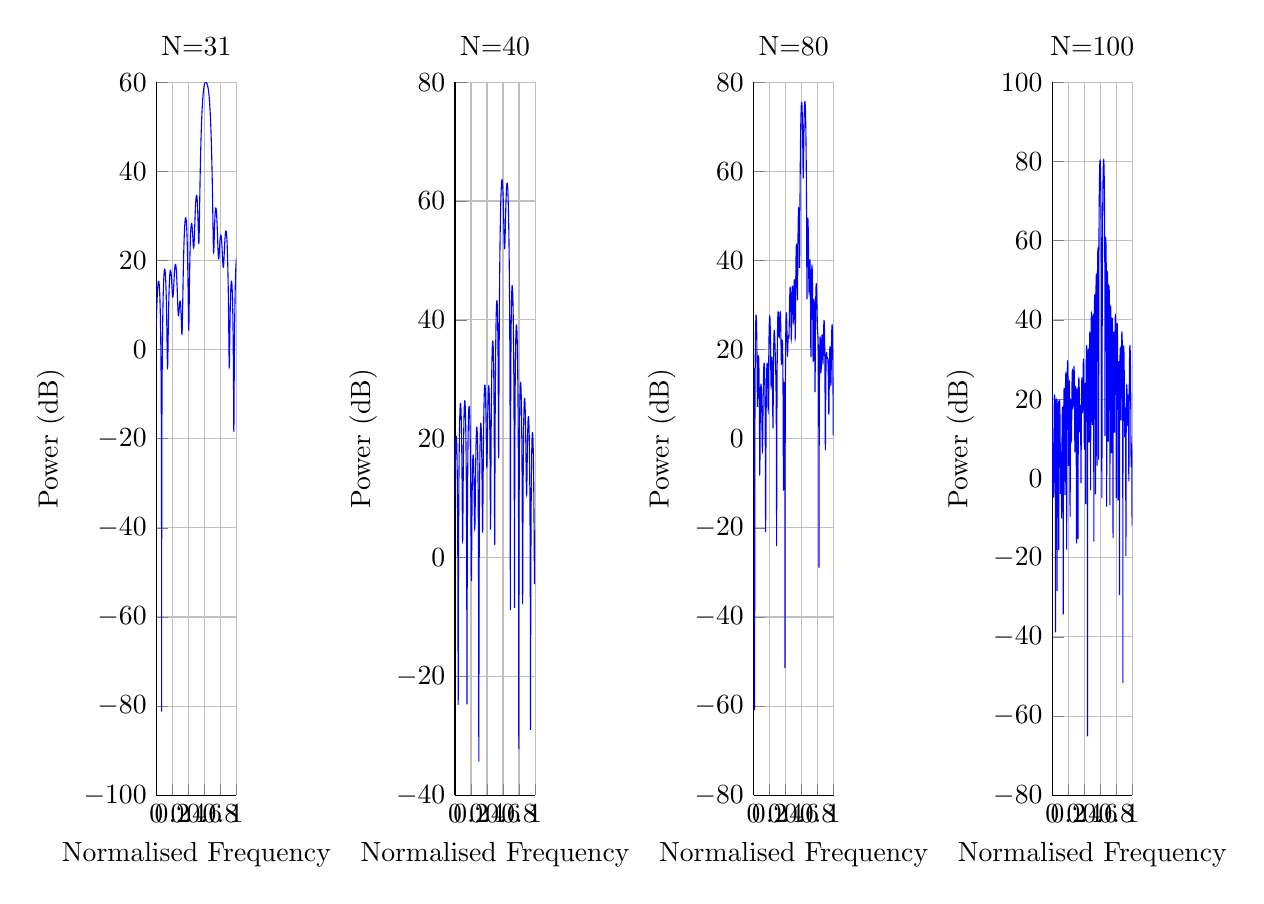
\begin{tikzpicture}

\begin{axis}[%
width=0.400265957446809in,
height=3.565625in,
scale only axis,
xmin=0,
xmax=1,
xlabel={Normalised Frequency},
xmajorgrids,
ymin=-40,
ymax=80,
ylabel={Power (dB)},
ymajorgrids,
name=plot2,
title={N=40},
axis x line*=bottom,
axis y line*=left
]
\addplot [color=blue,solid,forget plot]
  table[row sep=crcr]{-1	5.47923508540802\\
-0.99951171875	6.29642550452079\\
-0.9990234375	7.07604630830908\\
-0.99853515625	7.8181632669538\\
-0.998046875	8.52335458407455\\
-0.99755859375	9.19252067181034\\
-0.9970703125	9.82675198947961\\
-0.99658203125	10.427238161287\\
-0.99609375	10.9952062145705\\
-0.99560546875	11.5318792465667\\
-0.9951171875	12.0384493549956\\
-0.99462890625	12.5160604806614\\
-0.994140625	12.9657980983236\\
-0.99365234375	13.3886836023568\\
-0.9931640625	13.7856718752663\\
-0.99267578125	14.1576509788112\\
-0.9921875	14.5054432254801\\
-0.99169921875	14.8298071120191\\
-0.9912109375	15.1314397545209\\
-0.99072265625	15.4109795757933\\
-0.990234375	15.669009074066\\
-0.98974609375	15.906057557198\\
-0.9892578125	16.1226037651925\\
-0.98876953125	16.3190783307828\\
-0.98828125	16.4958660465017\\
-0.98779296875	16.6533079193719\\
-0.9873046875	16.7917030028502\\
-0.98681640625	16.9113100011178\\
-0.986328125	17.0123486441012\\
-0.98583984375	17.0950008333136\\
-0.9853515625	17.1594115591685\\
-0.98486328125	17.2056895901216\\
-0.984375	17.2339079330458\\
-0.98388671875	17.2441040627745\\
-0.9833984375	17.23627991684\\
-0.98291015625	17.2104016491209\\
-0.982421875	17.1663991334175\\
-0.98193359375	17.1041652048624\\
-0.9814453125	17.0235546235192\\
-0.98095703125	16.9243827404414\\
-0.98046875	16.8064238417821\\
-0.97998046875	16.66940914113\\
-0.9794921875	16.5130243839606\\
-0.97900390625	16.3369070207382\\
-0.978515625	16.1406428965589\\
-0.97802734375	15.9237623950008\\
-0.9775390625	15.6857359616876\\
-0.97705078125	15.4259689185407\\
-0.9765625	15.1437954622489\\
-0.97607421875	14.8384717194505\\
-0.9755859375	14.5091677056536\\
-0.97509765625	14.1549580039941\\
-0.974609375	13.7748109422353\\
-0.97412109375	13.3675760003847\\
-0.9736328125	12.9319691249762\\
-0.97314453125	12.4665555571109\\
-0.97265625	11.9697296969847\\
-0.97216796875	11.4396914247224\\
-0.9716796875	10.8744181725534\\
-0.97119140625	10.2716318937381\\
-0.970703125	9.62875989766785\\
-0.97021484375	8.94288832058973\\
-0.9697265625	8.21070678846963\\
-0.96923828125	7.42844263191891\\
-0.96875	6.59178289947621\\
-0.96826171875	5.69578252669392\\
-0.9677734375	4.73475764743721\\
-0.96728515625	3.70216477869104\\
-0.966796875	2.590470690127\\
-0.96630859375	1.39102668228407\\
-0.9658203125	0.0939799047554345\\
-0.96533203125	-1.31170597327688\\
-0.96484375	-2.8379652909011\\
-0.96435546875	-4.49675036345855\\
-0.9638671875	-6.29786337453249\\
-0.96337890625	-8.24406550765307\\
-0.962890625	-10.3206289497842\\
-0.96240234375	-12.4744194036897\\
-0.9619140625	-14.5771314812121\\
-0.96142578125	-16.3795932671628\\
-0.9609375	-17.5118586857787\\
-0.96044921875	-17.6341753448389\\
-0.9599609375	-16.6952847056059\\
-0.95947265625	-14.9796232753458\\
-0.958984375	-12.8719255881271\\
-0.95849609375	-10.6587097414189\\
-0.9580078125	-8.49700844265999\\
-0.95751953125	-6.45606048584405\\
-0.95703125	-4.5583745640846\\
-0.95654296875	-2.8045601777211\\
-0.9560546875	-1.18605311623711\\
-0.95556640625	0.308838105378672\\
-0.955078125	1.69220838461058\\
-0.95458984375	2.97541581641471\\
-0.9541015625	4.16867756188898\\
-0.95361328125	5.28099755559667\\
-0.953125	6.32023504083558\\
-0.95263671875	7.29322465753812\\
-0.9521484375	8.20590735396011\\
-0.95166015625	9.06345454992761\\
-0.951171875	9.87037894177624\\
-0.95068359375	10.6306304110712\\
-0.9501953125	11.3476777222062\\
-0.94970703125	12.024577549498\\
-0.94921875	12.6640325886059\\
-0.94873046875	13.2684404362094\\
-0.9482421875	13.8399347390883\\
-0.94775390625	14.3804199012921\\
-0.947265625	14.8916004329964\\
-0.94677734375	15.3750058416836\\
-0.9462890625	15.832011809577\\
-0.94580078125	16.2638582700236\\
-0.9453125	16.6716648870482\\
-0.94482421875	17.056444353282\\
-0.9443359375	17.4191138486911\\
-0.94384765625	17.7605049431089\\
-0.943359375	18.0813721770486\\
-0.94287109375	18.3824005155953\\
-0.9423828125	18.664211837669\\
-0.94189453125	18.9273705962425\\
-0.94140625	19.1723887630977\\
-0.94091796875	19.3997301535125\\
-0.9404296875	19.6098142111806\\
-0.93994140625	19.8030193210977\\
-0.939453125	19.9796857076325\\
-0.93896484375	20.1401179661708\\
-0.9384765625	20.2845872692607\\
-0.93798828125	20.4133332818582\\
-0.9375	20.5265658148634\\
-0.93701171875	20.6244662414861\\
-0.9365234375	20.707188696949\\
-0.93603515625	20.7748610785034\\
-0.935546875	20.8275858596146\\
-0.93505859375	20.8654407293703\\
-0.9345703125	20.8884790656255\\
-0.93408203125	20.8967302480368\\
-0.93359375	20.890199814925\\
-0.93310546875	20.8688694657603\\
-0.9326171875	20.8326969089658\\
-0.93212890625	20.7816155526105\\
-0.931640625	20.7155340333792\\
-0.93115234375	20.6343355769044\\
-0.9306640625	20.5378771800692\\
-0.93017578125	20.4259886031769\\
-0.9296875	20.2984711568608\\
-0.92919921875	20.1550962651915\\
-0.9287109375	19.9956037825275\\
-0.92822265625	19.8197000371291\\
-0.927734375	19.6270555692657\\
-0.92724609375	19.4173025253137\\
-0.9267578125	19.1900316619388\\
-0.92626953125	18.9447889056063\\
-0.92578125	18.681071402007\\
-0.92529296875	18.3983229770821\\
-0.9248046875	18.095928915604\\
-0.92431640625	17.773209943986\\
-0.923828125	17.4294152802117\\
-0.92333984375	17.0637145842457\\
-0.9228515625	16.6751886054038\\
-0.92236328125	16.2628182767658\\
-0.921875	15.8254719479599\\
-0.92138671875	15.3618903726801\\
-0.9208984375	14.8706689709078\\
-0.92041015625	14.3502367608438\\
-0.919921875	13.7988311921306\\
-0.91943359375	13.2144678962036\\
-0.9189453125	12.5949040819748\\
-0.91845703125	11.9375939174066\\
-0.91796875	11.2396337090945\\
-0.91748046875	10.4976939625626\\
-0.9169921875	9.70793438556514\\
-0.91650390625	8.86589644817291\\
-0.916015625	7.96636602426334\\
-0.91552734375	7.00319557303741\\
-0.9150390625	5.96907073294631\\
-0.91455078125	4.85519919435055\\
-0.9140625	3.65088876264179\\
-0.91357421875	2.34296394626053\\
-0.9130859375	0.914941373918007\\
-0.91259765625	-0.654165177211983\\
-0.912109375	-2.39162697183271\\
-0.91162109375	-4.33374802363803\\
-0.9111328125	-6.53026813537727\\
-0.91064453125	-9.05174291122221\\
-0.91015625	-12.0025706536052\\
-0.90966796875	-15.5453230303323\\
-0.9091796875	-19.9483804715371\\
-0.90869140625	-25.6747183054013\\
-0.908203125	-33.3932030237655\\
-0.90771484375	-41.1988316677108\\
-0.9072265625	-37.1215017671252\\
-0.90673828125	-28.6497137570833\\
-0.90625	-22.2056952309753\\
-0.90576171875	-17.3555118824721\\
-0.9052734375	-13.5272286618084\\
-0.90478515625	-10.3852507894733\\
-0.904296875	-7.73095190080696\\
-0.90380859375	-5.43976899744673\\
-0.9033203125	-3.42919309797641\\
-0.90283203125	-1.64201204973146\\
-0.90234375	-0.0370344357399\\
-0.90185546875	1.41633169662339\\
-0.9013671875	2.74140227893297\\
-0.90087890625	3.9563401523201\\
-0.900390625	5.07555989389737\\
-0.89990234375	6.11068620760513\\
-0.8994140625	7.07122528291142\\
-0.89892578125	7.96504609693886\\
-0.8984375	8.79873256897989\\
-0.89794921875	9.57784591957474\\
-0.8974609375	10.3071233061194\\
-0.89697265625	10.9906304012085\\
-0.896484375	11.6318801285935\\
-0.89599609375	12.2339261579934\\
-0.8955078125	12.7994373165086\\
-0.89501953125	13.3307573920269\\
-0.89453125	13.8299536264373\\
-0.89404296875	14.2988563596568\\
-0.8935546875	14.7390916825031\\
-0.89306640625	15.1521085163427\\
-0.892578125	15.5392012123924\\
-0.89208984375	15.9015285207984\\
-0.8916015625	16.240129596457\\
-0.89111328125	16.5559375690129\\
-0.890625	16.8497910972149\\
-0.89013671875	17.1224442446627\\
-0.8896484375	17.3745749490019\\
-0.88916015625	17.6067923054698\\
-0.888671875	17.8196428451131\\
-0.88818359375	18.013615955605\\
-0.8876953125	18.1891485665336\\
-0.88720703125	18.3466291999639\\
-0.88671875	18.486401469908\\
-0.88623046875	18.6087671002793\\
-0.8857421875	18.7139885193055\\
-0.88525390625	18.8022910787547\\
-0.884765625	18.873864938284\\
-0.88427734375	18.928866648456\\
-0.8837890625	18.967420460237\\
-0.88330078125	18.989619383891\\
-0.8828125	18.9955260159711\\
-0.88232421875	18.9851731494452\\
-0.8818359375	18.9585641787876\\
-0.88134765625	18.9156733090284\\
-0.880859375	18.8564455752299\\
-0.88037109375	18.7807966765913\\
-0.8798828125	18.6886126273426\\
-0.87939453125	18.5797492247556\\
-0.87890625	18.4540313329674\\
-0.87841796875	18.3112519798906\\
-0.8779296875	18.1511712633111\\
-0.87744140625	17.9735150614053\\
-0.876953125	17.7779735424455\\
-0.87646484375	17.5641994685431\\
-0.8759765625	17.3318062891164\\
-0.87548828125	17.0803660216706\\
-0.875	16.8094069208579\\
-0.87451171875	16.5184109422593\\
-0.8740234375	16.2068110157466\\
-0.87353515625	15.8739881558388\\
-0.873046875	15.5192684548608\\
-0.87255859375	15.1419200313361\\
-0.8720703125	14.7411500442768\\
-0.87158203125	14.3161019386938\\
-0.87109375	13.8658531655547\\
-0.87060546875	13.3894137303192\\
-0.8701171875	12.8857260819855\\
-0.86962890625	12.3536670791832\\
-0.869140625	11.7920530896847\\
-0.86865234375	11.1996497354058\\
-0.8681640625	10.5751884442791\\
-0.86767578125	9.91739289481654\\
-0.8671875	9.22501975212884\\
-0.86669921875	8.4969199496852\\
-0.8662109375	7.73212936990187\\
-0.86572265625	6.93000136066336\\
-0.865234375	6.09039833990348\\
-0.86474609375	5.21396592253661\\
-0.8642578125	4.3025203005617\\
-0.86376953125	3.35958676479012\\
-0.86328125	2.39113080687509\\
-0.86279296875	1.40651535536469\\
-0.8623046875	0.419683087148077\\
-0.86181640625	-0.549523965049394\\
-0.861328125	-1.47416606053138\\
-0.86083984375	-2.31965722838428\\
-0.8603515625	-3.0447011465201\\
-0.85986328125	-3.60465452124209\\
-0.859375	-3.95776036299476\\
-0.85888671875	-4.07330716770707\\
-0.8583984375	-3.93901210645995\\
-0.85791015625	-3.56429149936267\\
-0.857421875	-2.97773113189824\\
-0.85693359375	-2.22007191851076\\
-0.8564453125	-1.33596470420284\\
-0.85595703125	-0.367384511181452\\
-0.85546875	0.650112968031944\\
-0.85498046875	1.68860053576807\\
-0.8544921875	2.72737554671781\\
-0.85400390625	3.75181107876896\\
-0.853515625	4.75203268429366\\
-0.85302734375	5.72170989896038\\
-0.8525390625	6.6570676118907\\
-0.85205078125	7.55612627458793\\
-0.8515625	8.41814003416041\\
-0.85107421875	9.24319150150039\\
-0.8505859375	10.0319044661668\\
-0.85009765625	10.7852428142328\\
-0.849609375	11.5043712887615\\
-0.84912109375	12.1905600924355\\
-0.8486328125	12.845120326824\\
-0.84814453125	13.4693609982472\\
-0.84765625	14.0645610363031\\
-0.84716796875	14.6319517135814\\
-0.8466796875	15.1727062308372\\
-0.84619140625	15.687934201056\\
-0.845703125	16.1786794467224\\
-0.84521484375	16.6459200025125\\
-0.8447265625	17.0905695510591\\
-0.84423828125	17.5134797550047\\
-0.84375	17.9154431140864\\
-0.84326171875	18.2971960923613\\
-0.8427734375	18.6594223424819\\
-0.84228515625	19.0027559113718\\
-0.841796875	19.3277843519179\\
-0.84130859375	19.6350516934065\\
-0.8408203125	19.9250612429501\\
-0.84033203125	20.1982782035902\\
-0.83984375	20.4551321038782\\
-0.83935546875	20.6960190398217\\
-0.8388671875	20.9213037340037\\
-0.83837890625	21.1313214190999\\
-0.837890625	21.3263795543764\\
-0.83740234375	21.5067593843718\\
-0.8369140625	21.6727173490924\\
-0.83642578125	21.8244863548294\\
-0.8359375	21.9622769142672\\
-0.83544921875	22.0862781639679\\
-0.8349609375	22.196658766648\\
-0.83447265625	22.2935677049464\\
-0.833984375	22.3771349726404\\
-0.83349609375	22.4474721685249\\
-0.8330078125	22.5046729974223\\
-0.83251953125	22.5488136820594\\
-0.83203125	22.5799532888203\\
-0.83154296875	22.5981339696648\\
-0.8310546875	22.6033811217894\\
-0.83056640625	22.5957034658893\\
-0.830078125	22.575093043157\\
-0.82958984375	22.5415251304141\\
-0.8291015625	22.494958072008\\
-0.82861328125	22.4353330263082\\
-0.828125	22.3625736237949\\
-0.82763671875	22.2765855328326\\
-0.8271484375	22.1772559282492\\
-0.82666015625	22.0644528567853\\
-0.826171875	21.9380244923141\\
-0.82568359375	21.797798272446\\
-0.8251953125	21.6435799066969\\
-0.82470703125	21.4751522447894\\
-0.82421875	21.2922739918435\\
-0.82373046875	21.0946782551599\\
-0.8232421875	20.8820709049713\\
-0.82275390625	20.6541287288806\\
-0.822265625	20.4104973566809\\
-0.82177734375	20.1507889287917\\
-0.8212890625	19.8745794775943\\
-0.82080078125	19.5814059864322\\
-0.8203125	19.2707630858864\\
-0.81982421875	18.9420993410724\\
-0.8193359375	18.5948130770539\\
-0.81884765625	18.2282476819882\\
-0.818359375	17.8416863192767\\
-0.81787109375	17.4343459708334\\
-0.8173828125	17.0053707237534\\
-0.81689453125	16.5538242024721\\
-0.81640625	16.0786810385853\\
-0.81591796875	15.5788172619228\\
-0.8154296875	15.0529994911132\\
-0.81494140625	14.4998728028316\\
-0.814453125	13.9179471712811\\
-0.81396484375	13.3055824015147\\
-0.8134765625	12.6609715454241\\
-0.81298828125	11.9821229094436\\
-0.8125	11.2668409737457\\
-0.81201171875	10.5127069018076\\
-0.8115234375	9.71705992145808\\
-0.81103515625	8.87698185978458\\
-0.810546875	7.98928877241283\\
-0.81005859375	7.05053635086027\\
-0.8095703125	6.05705033287444\\
-0.80908203125	5.00500066594314\\
-0.80859375	3.89055064241491\\
-0.80810546875	2.71013281111518\\
-0.8076171875	1.46093711305553\\
-0.80712890625	0.141750393080023\\
-0.806640625	-1.24563200955595\\
-0.80615234375	-2.69409103229458\\
-0.8056640625	-4.18752242226394\\
-0.80517578125	-5.69540069372645\\
-0.8046875	-7.16563808423089\\
-0.80419921875	-8.51752215753594\\
-0.8037109375	-9.64017408050847\\
-0.80322265625	-10.4060601314432\\
-0.802734375	-10.7061531158657\\
-0.80224609375	-10.4949185439379\\
-0.8017578125	-9.81287094515617\\
-0.80126953125	-8.76640010675162\\
-0.80078125	-7.48313221387295\\
-0.80029296875	-6.07556447936825\\
-0.7998046875	-4.62631444983881\\
-0.79931640625	-3.18904175526501\\
-0.798828125	-1.79537625998138\\
-0.79833984375	-0.462132376637274\\
-0.7978515625	0.803139022369467\\
-0.79736328125	1.99839125093603\\
-0.796875	3.1246978029965\\
-0.79638671875	4.18479623203117\\
-0.7958984375	5.18222096412074\\
-0.79541015625	6.12079833256711\\
-0.794921875	7.00436056269425\\
-0.79443359375	7.83659063022554\\
-0.7939453125	8.62094456576069\\
-0.79345703125	9.36061900072007\\
-0.79296875	10.0585446087954\\
-0.79248046875	10.7173938585596\\
-0.7919921875	11.3395961765253\\
-0.79150390625	11.9273564489813\\
-0.791015625	12.4826745009554\\
-0.79052734375	13.0073642233872\\
-0.7900390625	13.5030716409713\\
-0.78955078125	13.9712915839128\\
-0.7890625	14.4133828446921\\
-0.78857421875	14.8305818255012\\
-0.7880859375	15.2240147498607\\
-0.78759765625	15.5947085455586\\
-0.787109375	15.9436005193345\\
-0.78662109375	16.2715469452118\\
-0.7861328125	16.5793306833034\\
-0.78564453125	16.8676679374698\\
-0.78515625	17.1372142503314\\
-0.78466796875	17.3885698239333\\
-0.7841796875	17.6222842444975\\
-0.78369140625	17.8388606804793\\
-0.783203125	18.0387596147531\\
-0.78271484375	18.2224021642074\\
-0.7822265625	18.390173033325\\
-0.78173828125	18.5424231424074\\
-0.78125	18.6794719658922\\
-0.78076171875	18.8016096116542\\
-0.7802734375	18.9090986681791\\
-0.77978515625	19.0021758430026\\
-0.779296875	19.0810534127373\\
-0.77880859375	19.1459205023202\\
-0.7783203125	19.1969442087431\\
-0.77783203125	19.2342705824375\\
-0.77734375	19.2580254776301\\
-0.77685546875	19.2683152813342\\
-0.7763671875	19.2652275291593\\
-0.77587890625	19.2488314147829\\
-0.775390625	19.2191781987093\\
-0.77490234375	19.1763015208165\\
-0.7744140625	19.1202176201502\\
-0.77392578125	19.0509254644359\\
-0.7734375	18.9684067908418\\
-0.77294921875	18.8726260586111\\
-0.7724609375	18.7635303132845\\
-0.77197265625	18.6410489613333\\
-0.771484375	18.5050934531114\\
-0.77099609375	18.3555568710927\\
-0.7705078125	18.1923134193762\\
-0.77001953125	18.0152178093988\\
-0.76953125	17.8241045356834\\
-0.76904296875	17.618787034243\\
-0.7685546875	17.3990567149533\\
-0.76806640625	17.1646818577662\\
-0.767578125	16.9154063610553\\
-0.76708984375	16.6509483286362\\
-0.7666015625	16.3709984800637\\
-0.76611328125	16.0752183666676\\
-0.765625	15.7632383734105\\
-0.76513671875	15.4346554840373\\
-0.7646484375	15.0890307841158\\
-0.76416015625	14.725886673454\\
-0.763671875	14.3447037560373\\
-0.76318359375	13.9449173721277\\
-0.7626953125	13.5259137336015\\
-0.76220703125	13.0870256201686\\
-0.76171875	12.6275275911125\\
-0.76123046875	12.1466306651116\\
-0.7607421875	11.6434764202973\\
-0.76025390625	11.117130469166\\
-0.759765625	10.5665752700862\\
-0.75927734375	9.99070225169982\\
-0.7587890625	9.38830325273073\\
-0.75830078125	8.75806132403191\\
-0.7578125	8.09854101198665\\
-0.75732421875	7.40817835776088\\
-0.7568359375	6.68527102864663\\
-0.75634765625	5.92796928178762\\
-0.755859375	5.13426890265095\\
-0.75537109375	4.302007947418\\
-0.7548828125	3.42887018532988\\
-0.75439453125	2.51239979545095\\
-0.75390625	1.55003445250739\\
-0.75341796875	0.539167951118318\\
-0.7529296875	-0.522740247291058\\
-0.75244140625	-1.63798153173321\\
-0.751953125	-2.80829902227894\\
-0.75146484375	-4.03440924915479\\
-0.7509765625	-5.31525002048074\\
-0.75048828125	-6.64681984938132\\
-0.75	-8.02043367930763\\
-0.74951171875	-9.42020921486223\\
-0.7490234375	-10.8196996237097\\
-0.74853515625	-12.1779729146297\\
-0.748046875	-13.4363596379693\\
-0.74755859375	-14.5186410934626\\
-0.7470703125	-15.3388000541436\\
-0.74658203125	-15.8190160853658\\
-0.74609375	-15.9137447070573\\
-0.74560546875	-15.6270496544732\\
-0.7451171875	-15.0109842130999\\
-0.74462890625	-14.1462444419489\\
-0.744140625	-13.1183597331722\\
-0.74365234375	-12.0012287713185\\
-0.7431640625	-10.8507913776975\\
-0.74267578125	-9.70561538188501\\
-0.7421875	-8.59038701423745\\
-0.74169921875	-7.51979548569095\\
-0.7412109375	-6.50177495144576\\
-0.74072265625	-5.53989055761531\\
-0.740234375	-4.63498116873998\\
-0.73974609375	-3.78624724992235\\
-0.7392578125	-2.99195373338864\\
-0.73876953125	-2.24987596870543\\
-0.73828125	-1.55757798024231\\
-0.73779296875	-0.912582698607316\\
-0.7373046875	-0.312473212588228\\
-0.73681640625	0.245049696830431\\
-0.736328125	0.762137493295144\\
-0.73583984375	1.24078087569903\\
-0.7353515625	1.68280715756286\\
-0.73486328125	2.08988378126569\\
-0.734375	2.46352526299324\\
-0.73388671875	2.80510186124653\\
-0.7333984375	3.11584890344645\\
-0.73291015625	3.3968761179756\\
-0.732421875	3.64917658393171\\
-0.73193359375	3.87363508001131\\
-0.7314453125	4.07103572091639\\
-0.73095703125	4.24206883625744\\
-0.73046875	4.38733708727453\\
-0.72998046875	4.50736084005858\\
-0.7294921875	4.60258282636334\\
-0.72900390625	4.67337212852696\\
-0.728515625	4.72002752605929\\
-0.72802734375	4.74278023981224\\
-0.7275390625	4.74179610645686\\
-0.72705078125	4.71717721199317\\
-0.7265625	4.66896300872373\\
-0.72607421875	4.59713093589908\\
-0.7255859375	4.50159656038322\\
-0.72509765625	4.38221325046911\\
-0.724609375	4.2387713937008\\
-0.72412109375	4.07099716862575\\
-0.7236328125	3.8785508813319\\
-0.72314453125	3.6610248811729\\
-0.72265625	3.4179410773186\\
-0.72216796875	3.14874809022399\\
-0.7216796875	2.85281809200671\\
-0.72119140625	2.52944342025416\\
-0.720703125	2.17783309557849\\
-0.72021484375	1.79710944099181\\
-0.7197265625	1.38630510063\\
-0.71923828125	0.944360900673682\\
-0.71875	0.470125207190549\\
-0.71826171875	-0.0376442557086591\\
-0.7177734375	-0.580274714302864\\
-0.71728515625	-1.15916671176494\\
-0.716796875	-1.77577350884515\\
-0.71630859375	-2.43156710323658\\
-0.7158203125	-3.12798442987046\\
-0.71533203125	-3.86634438089952\\
-0.71484375	-4.64772209897473\\
-0.71435546875	-5.47276110960043\\
-0.7138671875	-6.34139582405235\\
-0.71337890625	-7.25244656722777\\
-0.712890625	-8.20303725714562\\
-0.71240234375	-9.18777521215243\\
-0.7119140625	-10.1976315653964\\
-0.71142578125	-11.2184879966404\\
-0.7109375	-12.2294062955381\\
-0.71044921875	-13.2008853702789\\
-0.7099609375	-14.0937441367344\\
-0.70947265625	-14.8597634318734\\
-0.708984375	-15.4455275756077\\
-0.70849609375	-15.8003558544066\\
-0.7080078125	-15.8872051792859\\
-0.70751953125	-15.6926253748432\\
-0.70703125	-15.2307705164843\\
-0.70654296875	-14.5391631237062\\
-0.7060546875	-13.6686386809072\\
-0.70556640625	-12.6724858313007\\
-0.705078125	-11.5986296690182\\
-0.70458984375	-10.4859001128456\\
-0.7041015625	-9.36346019454841\\
-0.70361328125	-8.25195437003964\\
-0.703125	-7.16525766694213\\
-0.70263671875	-6.11220029904277\\
-0.7021484375	-5.09801128203508\\
-0.70166015625	-4.12542849106227\\
-0.701171875	-3.1955109008505\\
-0.70068359375	-2.30821477031558\\
-0.7001953125	-1.4627940649057\\
-0.69970703125	-0.658074638920121\\
-0.69921875	0.107360306325048\\
-0.69873046875	0.835046285644259\\
-0.6982421875	1.52655587954202\\
-0.69775390625	2.1834459678981\\
-0.697265625	2.80722458880872\\
-0.69677734375	3.3993310569248\\
-0.6962890625	3.96112497672205\\
-0.69580078125	4.49388116318961\\
-0.6953125	4.99878842793\\
-0.69482421875	5.47695083749487\\
-0.6943359375	5.92939049617839\\
-0.69384765625	6.35705121143908\\
-0.693359375	6.76080261039499\\
-0.69287109375	7.14144442035765\\
-0.6923828125	7.49971072561086\\
-0.69189453125	7.83627408063127\\
-0.69140625	8.15174940633721\\
-0.69091796875	8.44669762738097\\
-0.6904296875	8.72162902956448\\
-0.68994140625	8.97700633033745\\
-0.689453125	9.21324746424297\\
-0.68896484375	9.4307280906434\\
-0.6884765625	9.6297838341611\\
-0.68798828125	9.81071226974917\\
-0.6875	9.97377466468439\\
-0.68701171875	10.11919748941\\
-0.6865234375	10.2471737082933\\
-0.68603515625	10.3578638601775\\
-0.685546875	10.4513969372014\\
-0.68505859375	10.5278710688264\\
-0.6845703125	10.5873540163697\\
-0.68408203125	10.629883481646\\
-0.68359375	10.6554672315626\\
-0.68310546875	10.6640830387024\\
-0.6826171875	10.6556784360617\\
-0.68212890625	10.6301702821721\\
-0.681640625	10.5874441308105\\
-0.68115234375	10.527353397382\\
-0.6806640625	10.4497183118144\\
-0.68017578125	10.3543246454296\\
-0.6796875	10.2409221967318\\
-0.67919921875	10.1092230183689\\
-0.6787109375	9.95889936468894\\
-0.67822265625	9.78958133633902\\
-0.677734375	9.60085419528696\\
-0.67724609375	9.39225532056765\\
-0.6767578125	9.16327077210624\\
-0.67626953125	8.91333142737829\\
-0.67578125	8.64180865379883\\
-0.67529296875	8.34800947914356\\
-0.6748046875	8.03117122386419\\
-0.67431640625	7.69045556416432\\
-0.673828125	7.32494200513586\\
-0.67333984375	6.93362076209568\\
-0.6728515625	6.51538508001283\\
-0.67236328125	6.06902307237743\\
-0.671875	5.59320924233447\\
-0.67138671875	5.08649597602933\\
-0.6708984375	4.54730549472951\\
-0.67041015625	3.97392305486163\\
-0.669921875	3.36449264962264\\
-0.66943359375	2.71701717849891\\
-0.6689453125	2.02936614489102\\
-0.66845703125	1.2992956224139\\
-0.66796875	0.524487813205937\\
-0.66748046875	-0.297378511246143\\
-0.6669921875	-1.16850932188066\\
-0.66650390625	-2.09080180180264\\
-0.666015625	-3.06553557174811\\
-0.66552734375	-4.09288821703204\\
-0.6650390625	-5.17118715467088\\
-0.66455078125	-6.29577637927923\\
-0.6640625	-7.45734704541386\\
-0.66357421875	-8.6395864817823\\
-0.6630859375	-9.81611739607176\\
-0.66259765625	-10.9470758321871\\
-0.662109375	-11.9765087809494\\
-0.66162109375	-12.8330718943424\\
-0.6611328125	-13.437481949736\\
-0.66064453125	-13.7186914487545\\
-0.66015625	-13.6349350024911\\
-0.65966796875	-13.1888288478166\\
-0.6591796875	-12.4263579364875\\
-0.65869140625	-11.4204825271014\\
-0.658203125	-10.2501967304115\\
-0.65771484375	-8.98528523552226\\
-0.6572265625	-7.67979076252642\\
-0.65673828125	-6.37185270794074\\
-0.65625	-5.08649887902668\\
-0.65576171875	-3.83906556112938\\
-0.6552734375	-2.63818562687153\\
-0.65478515625	-1.48805771088304\\
-0.654296875	-0.390047364303797\\
-0.65380859375	0.6562301682458\\
-0.6533203125	1.6521969388922\\
-0.65283203125	2.5998514666598\\
-0.65234375	3.50147558643713\\
-0.65185546875	4.35945113637281\\
-0.6513671875	5.1761479136488\\
-0.65087890625	5.95385754031219\\
-0.650390625	6.69475669199502\\
-0.64990234375	7.4008889344399\\
-0.6494140625	8.07415819354487\\
-0.64892578125	8.71632934566964\\
-0.6484375	9.32903301616321\\
-0.64794921875	9.91377271653175\\
-0.6474609375	10.4719331299246\\
-0.64697265625	11.0047887973775\\
-0.646484375	11.513512745632\\
-0.64599609375	11.9991847846965\\
-0.6455078125	12.4627993243812\\
-0.64501953125	12.9052726365697\\
-0.64453125	13.3274495388959\\
-0.64404296875	13.7301095056187\\
-0.6435546875	14.1139722293091\\
-0.64306640625	14.4797026667966\\
-0.642578125	14.8279156075042\\
-0.64208984375	15.1591798037264\\
-0.6416015625	15.4740217018197\\
-0.64111328125	15.7729288115033\\
-0.640625	16.0563527480466\\
-0.64013671875	16.3247119793944\\
-0.6396484375	16.5783943074778\\
-0.63916015625	16.8177591102035\\
-0.638671875	17.0431393679983\\
-0.63818359375	17.2548434963448\\
-0.6376953125	17.4531570034991\\
-0.63720703125	17.6383439905406\\
-0.63671875	17.8106485090534\\
-0.63623046875	17.9702957900822\\
-0.6357421875	18.1174933565131\\
-0.63525390625	18.2524320297002\\
-0.634765625	18.3752868399712\\
-0.63427734375	18.486217849585\\
-0.6337890625	18.5853708957717\\
-0.63330078125	18.6728782606423\\
-0.6328125	18.7488592740073\\
-0.63232421875	18.8134208544734\\
-0.6318359375	18.8666579935918\\
-0.63134765625	18.9086541872968\\
-0.630859375	18.9394818183986\\
-0.63037109375	18.9592024934672\\
-0.6298828125	18.9678673370616\\
-0.62939453125	18.9655172459186\\
-0.62890625	18.9521831054088\\
-0.62841796875	18.9278859702926\\
-0.6279296875	18.8926372115679\\
-0.62744140625	18.846438630982\\
-0.626953125	18.7892825445904\\
-0.62646484375	18.7211518365787\\
-0.6259765625	18.6420199844221\\
-0.62548828125	18.5518510563371\\
-0.625	18.4505996818893\\
-0.62451171875	18.338210996554\\
-0.6240234375	18.2146205609883\\
-0.62353515625	18.0797542557728\\
-0.623046875	17.9335281524112\\
-0.62255859375	17.7758483614585\\
-0.6220703125	17.6066108587775\\
-0.62158203125	17.4257012911201\\
-0.62109375	17.2329947625011\\
-0.62060546875	17.0283556031995\\
-0.6201171875	16.811637123703\\
-0.61962890625	16.5826813565385\\
-0.619140625	16.341318789728\\
-0.61865234375	16.0873680966307\\
-0.6181640625	15.8206358682214\\
-0.61767578125	15.5409163554789\\
-0.6171875	15.2479912316072\\
-0.61669921875	14.9416293863781\\
-0.6162109375	14.62158676811\\
-0.61572265625	14.2876062928323\\
-0.615234375	13.9394178452519\\
-0.61474609375	13.576738402475\\
-0.6142578125	13.1992723193858\\
-0.61376953125	12.8067118245366\\
-0.61328125	12.3987377878801\\
-0.61279296875	11.9750208373015\\
-0.6123046875	11.5352229204938\\
-0.61181640625	11.078999433235\\
-0.611328125	10.6060020658029\\
-0.61083984375	10.115882557591\\
-0.6103515625	9.60829759776345\\
-0.60986328125	9.08291516916965\\
-0.609375	8.53942270620718\\
-0.60888671875	7.97753752765797\\
-0.6083984375	7.39702011564106\\
-0.60791015625	6.79769094442213\\
-0.607421875	6.17945171976149\\
-0.60693359375	5.54231207061519\\
-0.6064453125	4.8864229362654\\
-0.60595703125	4.2121181021742\\
-0.60546875	3.51996553382757\\
-0.60498046875	2.81083029684475\\
-0.6044921875	2.08595086076187\\
-0.60400390625	1.3470303457003\\
-0.603515625	0.59634360653668\\
-0.60302734375	-0.163140298738624\\
-0.6025390625	-0.92762308180573\\
-0.60205078125	-1.69233626022552\\
-0.6015625	-2.45140647522055\\
-0.60107421875	-3.19774685260785\\
-0.6005859375	-3.92300322462712\\
-0.60009765625	-4.61759306048778\\
-0.599609375	-5.27088076873576\\
-0.59912109375	-5.87153062343306\\
-0.5986328125	-6.40806199334352\\
-0.59814453125	-6.86959664299306\\
-0.59765625	-7.24673656050614\\
-0.59716796875	-7.53245505673155\\
-0.5966796875	-7.72284538236772\\
-0.59619140625	-7.81757276540124\\
-0.595703125	-7.81992784943371\\
-0.59521484375	-7.73646914262799\\
-0.5947265625	-7.57633646969609\\
-0.59423828125	-7.35038111390832\\
-0.59375	-7.07027250443443\\
-0.59326171875	-6.74771098168909\\
-0.5927734375	-6.39382249761013\\
-0.59228515625	-6.01875712154311\\
-0.591796875	-5.6314736632845\\
-0.59130859375	-5.23967178037088\\
-0.5908203125	-4.84982751860162\\
-0.59033203125	-4.46729251874758\\
-0.58984375	-4.09642571991658\\
-0.58935546875	-3.74073564243638\\
-0.5888671875	-3.40301933301043\\
-0.58837890625	-3.08549014399088\\
-0.587890625	-2.78989073964772\\
-0.58740234375	-2.51759041698389\\
-0.5869140625	-2.26966740278341\\
-0.58642578125	-2.04697760219278\\
-0.5859375	-1.85021160557345\\
-0.58544921875	-1.67994180712066\\
-0.5849609375	-1.53666138237139\\
-0.58447265625	-1.42081669516375\\
-0.583984375	-1.33283450746515\\
-0.58349609375	-1.2731451755849\\
-0.5830078125	-1.24220284798046\\
-0.58251953125	-1.24050353956552\\
-0.58203125	-1.26860184723133\\
-0.58154296875	-1.32712699127506\\
-0.5810546875	-1.41679881709886\\
-0.58056640625	-1.53844437074733\\
-0.580078125	-1.69301567148319\\
-0.57958984375	-1.88160934712159\\
-0.5791015625	-2.10548887793301\\
-0.57861328125	-2.36611032026858\\
-0.578125	-2.66515256350316\\
-0.57763671875	-3.0045534311566\\
-0.5771484375	-3.38655329540257\\
-0.57666015625	-3.81374837249644\\
-0.576171875	-4.28915656298603\\
-0.57568359375	-4.81629968251719\\
-0.5751953125	-5.39930733086054\\
-0.57470703125	-6.04304967787988\\
-0.57421875	-6.75330943886618\\
-0.57373046875	-7.53700781069883\\
-0.5732421875	-8.40250605102884\\
-0.57275390625	-9.36001526225763\\
-0.572265625	-10.4221645523228\\
-0.57177734375	-11.6048071632513\\
-0.5712890625	-12.9281951142563\\
-0.57080078125	-14.4187449374176\\
-0.5703125	-16.1117916550324\\
-0.56982421875	-18.0560791737693\\
-0.5693359375	-20.3214928090677\\
-0.56884765625	-23.0133243732507\\
-0.568359375	-26.3010650322043\\
-0.56787109375	-30.4841372078543\\
-0.5673828125	-36.1717745682147\\
-0.56689453125	-44.949366337071\\
-0.56640625	-64.3283388801126\\
-0.56591796875	-62.7535623085687\\
-0.5654296875	-43.9542573778939\\
-0.56494140625	-35.0100038469157\\
-0.564453125	-29.0487072941191\\
-0.56396484375	-24.5558017181555\\
-0.5634765625	-20.941226063873\\
-0.56298828125	-17.9128108222484\\
-0.5625	-15.3043430899915\\
-0.56201171875	-13.0121710716777\\
-0.5615234375	-10.9672717309155\\
-0.56103515625	-9.12135425297557\\
-0.560546875	-7.43930356623837\\
-0.56005859375	-5.8947812904133\\
-0.5595703125	-4.46752231726959\\
-0.55908203125	-3.14159853736136\\
-0.55859375	-1.90426209152574\\
-0.55810546875	-0.745150478957469\\
-0.5576171875	0.344274357552919\\
-0.55712890625	1.37113104368097\\
-0.556640625	2.3414171573341\\
-0.55615234375	3.26023299449425\\
-0.5556640625	4.13195204802822\\
-0.55517578125	4.96035273824779\\
-0.5546875	5.74872150640774\\
-0.55419921875	6.49993443169629\\
-0.5537109375	7.21652252644168\\
-0.55322265625	7.9007244759438\\
-0.552734375	8.55452961256599\\
-0.55224609375	9.17971321613941\\
-0.5517578125	9.77786572764624\\
-0.55126953125	10.3504170927911\\
-0.55078125	10.8986571773063\\
-0.55029296875	11.4237529897779\\
-0.5498046875	11.9267632916765\\
-0.54931640625	12.4086510549095\\
-0.548828125	12.870294135122\\
-0.54833984375	13.3124944573546\\
-0.5478515625	13.7359859545196\\
-0.54736328125	14.141441454839\\
-0.546875	14.5294786791451\\
-0.54638671875	14.9006654807546\\
-0.5458984375	15.2555244379302\\
-0.54541015625	15.5945368905645\\
-0.544921875	15.9181464977552\\
-0.54443359375	16.2267623806962\\
-0.5439453125	16.520761905227\\
-0.54345703125	16.8004931500546\\
-0.54296875	17.0662770997428\\
-0.54248046875	17.3184095957889\\
-0.5419921875	17.5571630742707\\
-0.54150390625	17.7827881144742\\
-0.541015625	17.9955148194676\\
-0.54052734375	18.1955540466673\\
-0.5400390625	18.3830985039468\\
-0.53955078125	18.5583237247069\\
-0.5390625	18.7213889334859\\
-0.53857421875	18.8724378121042\\
-0.5380859375	19.0115991749525\\
-0.53759765625	19.1389875608299\\
-0.537109375	19.254703747673\\
-0.53662109375	19.358835195579\\
-0.5361328125	19.4514564226838\\
-0.53564453125	19.5326293177003\\
-0.53515625	19.6024033922331\\
-0.53466796875	19.6608159753519\\
-0.5341796875	19.7078923523156\\
-0.53369140625	19.7436458487805\\
-0.533203125	19.7680778612926\\
-0.53271484375	19.781177834339\\
-0.5322265625	19.7829231837233\\
-0.53173828125	19.7732791655048\\
-0.53125	19.7521986892126\\
-0.53076171875	19.719622073494\\
-0.5302734375	19.67547674177\\
-0.52978515625	19.6196768548535\\
-0.529296875	19.5521228768034\\
-0.52880859375	19.4727010695549\\
-0.5283203125	19.3812829110419\\
-0.52783203125	19.2777244306209\\
-0.52734375	19.1618654545726\\
-0.52685546875	19.0335287532967\\
-0.5263671875	18.8925190804918\\
-0.52587890625	18.7386220930867\\
-0.525390625	18.5716031389483\\
-0.52490234375	18.3912058973571\\
-0.5244140625	18.1971508548975\\
-0.52392578125	17.9891335966562\\
-0.5234375	17.766822889412\\
-0.52294921875	17.5298585297111\\
-0.5224609375	17.2778489252573\\
-0.52197265625	17.0103683727498\\
-0.521484375	16.726953989001\\
-0.52099609375	16.427102244641\\
-0.5205078125	16.1102650406866\\
-0.52001953125	15.775845257389\\
-0.51953125	15.4231916916287\\
-0.51904296875	15.0515932831718\\
-0.5185546875	14.6602725106406\\
-0.51806640625	14.2483778142071\\
-0.517578125	13.8149748726814\\
-0.51708984375	13.3590365263765\\
-0.5166015625	12.8794310920557\\
-0.51611328125	12.3749087599734\\
-0.515625	11.8440856923904\\
-0.51513671875	11.2854253538766\\
-0.5146484375	10.6972164908519\\
-0.51416015625	10.0775470341356\\
-0.513671875	9.42427301456163\\
-0.51318359375	8.73498134594452\\
-0.5126953125	8.00694502625321\\
-0.51220703125	7.23706891687649\\
-0.51171875	6.42182375672779\\
-0.51123046875	5.55716542394323\\
-0.5107421875	4.63843564383825\\
-0.51025390625	3.66023933845314\\
-0.509765625	2.61629263873562\\
-0.50927734375	1.49923435727448\\
-0.5087890625	0.30039283064608\\
-0.50830078125	-0.990499498586216\\
-0.5078125	-2.3856470471761\\
-0.50732421875	-3.8995764784462\\
-0.5068359375	-5.54951578630343\\
-0.50634765625	-7.35561422458166\\
-0.505859375	-9.3405920104275\\
-0.50537109375	-11.5277577832612\\
-0.5048828125	-13.9346984130813\\
-0.50439453125	-16.5559881734491\\
-0.50390625	-19.3199673943034\\
-0.50341796875	-21.9961349097272\\
-0.5029296875	-24.070046027801\\
-0.50244140625	-24.8184121900723\\
-0.501953125	-23.8972550923352\\
-0.50146484375	-21.7551181735486\\
-0.5009765625	-19.1091303161655\\
-0.50048828125	-16.4257835006231\\
-0.5	-13.9033055163494\\
-0.49951171875	-11.5988884611366\\
-0.4990234375	-9.51261291187044\\
-0.49853515625	-7.6253327210705\\
-0.498046875	-5.91360762586154\\
-0.49755859375	-4.35506846800704\\
-0.4970703125	-2.93003744589792\\
-0.49658203125	-1.62174707221984\\
-0.49609375	-0.416078980511447\\
-0.49560546875	0.698822236615859\\
-0.4951171875	1.73292946408352\\
-0.49462890625	2.69466573944185\\
-0.494140625	3.59118130779501\\
-0.49365234375	4.42857943000821\\
-0.4931640625	5.21209880382379\\
-0.49267578125	5.94626060452113\\
-0.4921875	6.6349871691632\\
-0.49169921875	7.28169811728521\\
-0.4912109375	7.88938854832353\\
-0.49072265625	8.46069298159393\\
-0.490234375	8.99793791792206\\
-0.48974609375	9.50318528125043\\
-0.4892578125	9.97826851410475\\
-0.48876953125	10.4248227244955\\
-0.48828125	10.8443099897533\\
-0.48779296875	11.2380406957491\\
-0.4873046875	11.6071916129282\\
-0.48681640625	11.9528212720278\\
-0.486328125	12.2758830934119\\
-0.48583984375	12.5772366379005\\
-0.4853515625	12.8576572786429\\
-0.48486328125	13.1178445390603\\
-0.484375	13.3584292981476\\
-0.48388671875	13.5799800291555\\
-0.4833984375	13.7830082090927\\
-0.48291015625	13.967973013195\\
-0.482421875	14.1352853894272\\
-0.48193359375	14.2853115923678\\
-0.4814453125	14.4183762428037\\
-0.48095703125	14.5347649685082\\
-0.48046875	14.6347266725667\\
-0.47998046875	14.7184754679164\\
-0.4794921875	14.7861923102026\\
-0.47900390625	14.8380263554101\\
-0.478515625	14.8740960638148\\
-0.47802734375	14.8944900674721\\
-0.4775390625	14.8992678145882\\
-0.47705078125	14.8884600005969\\
-0.4765625	14.8620687924936\\
-0.47607421875	14.8200678498779\\
-0.4755859375	14.7624021431443\\
-0.47509765625	14.6889875662637\\
-0.474609375	14.5997103385417\\
-0.47412109375	14.4944261865502\\
-0.4736328125	14.3729592940161\\
-0.47314453125	14.2351010037419\\
-0.47265625	14.0806082515074\\
-0.47216796875	13.9092017072634\\
-0.4716796875	13.7205635936266\\
-0.47119140625	13.5143351455661\\
-0.470703125	13.2901136680389\\
-0.47021484375	13.0474491399479\\
-0.4697265625	12.7858403028663\\
-0.46923828125	12.5047301611502\\
-0.46875	12.203500805884\\
-0.46826171875	11.8814674580388\\
-0.4677734375	11.5378716055609\\
-0.46728515625	11.1718730839955\\
-0.466796875	10.7825409195852\\
-0.46630859375	10.3688427162066\\
-0.4658203125	9.92963232128123\\
-0.46533203125	9.46363544876047\\
-0.46484375	8.96943286671233\\
-0.46435546875	8.4454406695589\\
-0.4638671875	7.88988704648335\\
-0.46337890625	7.30078482297824\\
-0.462890625	6.67589888623767\\
-0.46240234375	6.01270740102411\\
-0.4619140625	5.30835547540568\\
-0.46142578125	4.5595996431664\\
-0.4609375	3.76274119813463\\
-0.46044921875	2.91354607148433\\
-0.4599609375	2.00714865615495\\
-0.45947265625	1.03793691543147\\
-0.458984375	-0.000583377299201419\\
-0.45849609375	-1.11594556644737\\
-0.4580078125	-2.31689567472832\\
-0.45751953125	-3.61356675011348\\
-0.45703125	-5.01761282025099\\
-0.45654296875	-6.5422054639201\\
-0.4560546875	-8.20167347660913\\
-0.45556640625	-10.0102969634225\\
-0.455078125	-11.9791792586267\\
-0.45458984375	-14.1088728861174\\
-0.4541015625	-16.3730382627527\\
-0.45361328125	-18.6851679570287\\
-0.453125	-20.8426796946288\\
-0.45263671875	-22.4767951904051\\
-0.4521484375	-23.1290650061452\\
-0.45166015625	-22.5566500880082\\
-0.451171875	-20.9655952229944\\
-0.45068359375	-18.8100322248495\\
-0.4501953125	-16.4733526076969\\
-0.44970703125	-14.1718500145493\\
-0.44921875	-11.9999371159328\\
-0.44873046875	-9.98768770402856\\
-0.4482421875	-8.13609566107218\\
-0.44775390625	-6.43458403576047\\
-0.447265625	-4.86895275523522\\
-0.44677734375	-3.42477062020727\\
-0.4462890625	-2.08869887239221\\
-0.44580078125	-0.848902367278199\\
-0.4453125	0.304926324787455\\
-0.44482421875	1.38169366714817\\
-0.4443359375	2.38907816050773\\
-0.44384765625	3.33370496093236\\
-0.443359375	4.22130470350482\\
-0.44287109375	5.05685131052354\\
-0.4423828125	5.84467880179095\\
-0.44189453125	6.58857916364664\\
-0.44140625	7.29188392527546\\
-0.44091796875	7.95753205734212\\
-0.4404296875	8.58812653244007\\
-0.43994140625	9.1859815440777\\
-0.439453125	9.75316204673684\\
-0.43896484375	10.2915169829905\\
-0.4384765625	10.8027073123686\\
-0.43798828125	11.2882297489199\\
-0.4375	11.7494369450235\\
-0.43701171875	12.1875547218914\\
-0.4365234375	12.6036968366019\\
-0.43603515625	12.9988776863861\\
-0.435546875	13.3740232790308\\
-0.43505859375	13.7299807402237\\
-0.4345703125	14.0675265816867\\
-0.43408203125	14.3873739157888\\
-0.43359375	14.6901787712653\\
-0.43310546875	14.9765456392696\\
-0.4326171875	15.2470323581626\\
-0.43212890625	15.5021544282998\\
-0.431640625	15.7423888339213\\
-0.43115234375	15.9681774375121\\
-0.4306640625	16.1799300022406\\
-0.43017578125	16.3780268899362\\
-0.4296875	16.5628214752421\\
-0.42919921875	16.7346423108527\\
-0.4287109375	16.8937950739093\\
-0.42822265625	17.0405643195481\\
-0.427734375	17.175215064132\\
-0.42724609375	17.2979942177526\\
-0.4267578125	17.4091318830835\\
-0.42626953125	17.5088425355182\\
-0.42578125	17.5973260976928\\
-0.42529296875	17.6747689199144\\
-0.4248046875	17.7413446766621\\
-0.42431640625	17.7972151881575\\
-0.423828125	17.8425311749948\\
-0.42333984375	17.8774329529483\\
-0.4228515625	17.9020510743225\\
-0.42236328125	17.9165069215589\\
-0.421875	17.9209132582505\\
-0.42138671875	17.9153747422264\\
-0.4208984375	17.8999884049531\\
-0.42041015625	17.8748441011335\\
-0.419921875	17.8400249320791\\
-0.41943359375	17.7956076461647\\
-0.4189453125	17.7416630194543\\
-0.41845703125	17.6782562194009\\
-0.41796875	17.6054471543681\\
-0.41748046875	17.523290811604\\
-0.4169921875	17.4318375861968\\
-0.41650390625	17.3311336034786\\
-0.416015625	17.2212210372942\\
-0.41552734375	17.1021384265325\\
-0.4150390625	16.9739209923116\\
-0.41455078125	16.8366009582325\\
-0.4140625	16.690207876147\\
-0.41357421875	16.5347689599454\\
-0.4130859375	16.3703094299364\\
-0.41259765625	16.1968528704837\\
-0.412109375	16.0144216036595\\
-0.41162109375	15.8230370817969\\
-0.4111328125	15.6227203019425\\
-0.41064453125	15.4134922453507\\
-0.41015625	15.1953743452977\\
-0.40966796875	14.9683889866398\\
-0.4091796875	14.7325600406788\\
-0.40869140625	14.4879134390297\\
-0.408203125	14.2344777903037\\
-0.40771484375	13.9722850435091\\
-0.4072265625	13.7013712021296\\
-0.40673828125	13.4217770928417\\
-0.40625	13.1335491927755\\
-0.40576171875	12.8367405190688\\
-0.4052734375	12.5314115842071\\
-0.40478515625	12.2176314202404\\
-0.404296875	11.8954786743913\\
-0.40380859375	11.5650427777831\\
-0.4033203125	11.2264251879682\\
-0.40283203125	10.8797407045829\\
-0.40234375	10.5251188557335\\
-0.40185546875	10.1627053505708\\
-0.4013671875	9.79266359086645\\
-0.40087890625	9.41517623120146\\
-0.400390625	9.03044677354398\\
-0.39990234375	8.63870117746871\\
-0.3994140625	8.24018946200372\\
-0.39892578125	7.83518726904879\\
-0.3984375	7.42399735149167\\
-0.39794921875	7.00695094159084\\
-0.3974609375	6.58440894699249\\
-0.39697265625	6.15676291307142\\
-0.396484375	5.72443568139135\\
-0.39599609375	5.28788166533699\\
-0.3955078125	4.8475866558719\\
-0.39501953125	4.4040670635578\\
-0.39453125	3.95786849820186\\
-0.39404296875	3.50956358568355\\
-0.3935546875	3.05974892366391\\
-0.39306640625	2.60904108504957\\
-0.392578125	2.1580715913197\\
-0.39208984375	1.7074807980218\\
-0.3916015625	1.25791066255255\\
-0.39111328125	0.809996399983155\\
-0.390625	0.364357075817257\\
-0.39013671875	-0.0784147658878561\\
-0.3896484375	-0.517764286543418\\
-0.38916015625	-0.953186140859943\\
-0.388671875	-1.38423660605628\\
-0.38818359375	-1.81054574176872\\
-0.3876953125	-2.23182923193176\\
-0.38720703125	-2.64789953621272\\
-0.38671875	-3.05867597269785\\
-0.38623046875	-3.46419336765283\\
-0.3857421875	-3.86460894282299\\
-0.38525390625	-4.26020716439708\\
-0.384765625	-4.65140234684963\\
-0.38427734375	-5.03873888389909\\
-0.3837890625	-5.42288906077695\\
-0.38330078125	-5.8046484789953\\
-0.3828125	-6.18492918872742\\
-0.38232421875	-6.56475066710688\\
-0.3818359375	-6.94522879648798\\
-0.38134765625	-7.32756297946227\\
-0.380859375	-7.7130214728147\\
-0.38037109375	-8.1029249270542\\
-0.3798828125	-8.49862797829987\\
-0.37939453125	-8.90149855122599\\
-0.37890625	-9.31289429020505\\
-0.37841796875	-9.73413523346429\\
-0.3779296875	-10.1664714724584\\
-0.37744140625	-10.6110440844552\\
-0.376953125	-11.0688370794432\\
-0.37646484375	-11.5406174564975\\
-0.3759765625	-12.0268597269754\\
-0.37548828125	-12.5276504696928\\
-0.375	-13.0425677324919\\
-0.37451171875	-13.5705295865526\\
-0.3740234375	-14.1096062528213\\
-0.37353515625	-14.6567916100269\\
-0.373046875	-15.20773361245\\
-0.37255859375	-15.7564307264796\\
-0.3720703125	-16.2949148792393\\
-0.37158203125	-16.8129624495595\\
-0.37109375	-17.2979039360197\\
-0.37060546875	-17.7346364937336\\
-0.3701171875	-18.1059702576835\\
-0.36962890625	-18.3934376859334\\
-0.369140625	-18.578636606613\\
-0.36865234375	-18.6450427552195\\
-0.3681640625	-18.5800337024594\\
-0.36767578125	-18.3766883559625\\
-0.3671875	-18.03487712658\\
-0.36669921875	-17.5613119752819\\
-0.3662109375	-16.9685410000201\\
-0.36572265625	-16.2731955040585\\
-0.365234375	-15.4939694121223\\
-0.36474609375	-14.6497778946944\\
-0.3642578125	-13.7583710130497\\
-0.36376953125	-12.8354818666498\\
-0.36328125	-11.8944472000656\\
-0.36279296875	-10.9461736417176\\
-0.3623046875	-9.99931723390192\\
-0.36181640625	-9.06056915608017\\
-0.361328125	-8.13497408359788\\
-0.36083984375	-7.22623733843946\\
-0.3603515625	-6.33699874376323\\
-0.35986328125	-5.46906507561787\\
-0.359375	-4.62360100739291\\
-0.35888671875	-3.80128242812972\\
-0.3583984375	-3.00241756191165\\
-0.35791015625	-2.22704151463071\\
-0.357421875	-1.47498941342783\\
-0.35693359375	-0.745952582288505\\
-0.3564453125	-0.0395214288187657\\
-0.35595703125	0.644781994544591\\
-0.35546875	1.3074794057702\\
-0.35498046875	1.94911784401693\\
-0.3544921875	2.57025592468342\\
-0.35400390625	3.17145369186559\\
-0.353515625	3.75326521534002\\
-0.35302734375	4.31623327645134\\
-0.3525390625	4.86088563969207\\
-0.35205078125	5.38773252412645\\
-0.3515625	5.89726497899563\\
-0.35107421875	6.38995393707191\\
-0.3505859375	6.86624977244361\\
-0.35009765625	7.32658223016766\\
-0.349609375	7.77136062650323\\
-0.34912109375	8.20097424245413\\
-0.3486328125	8.61579285179633\\
-0.34814453125	9.01616733894114\\
-0.34765625	9.40243037288375\\
-0.34716796875	9.77489711186074\\
-0.3466796875	10.1338659197795\\
-0.34619140625	10.4796190804234\\
-0.345703125	10.8124234992282\\
-0.34521484375	11.1325313853284\\
-0.3447265625	11.4401809087835\\
-0.34423828125	11.7355968295818\\
-0.34375	12.0189910962925\\
-0.34326171875	12.2905634131905\\
-0.3427734375	12.5505017753935\\
-0.34228515625	12.7989829720709\\
-0.341796875	13.0361730581598\\
-0.34130859375	13.2622277952879\\
-0.3408203125	13.4772930627809\\
-0.34033203125	13.681505239741\\
-0.33984375	13.8749915592466\\
-0.33935546875	14.0578704357454\\
-0.3388671875	14.2302517667054\\
-0.33837890625	14.3922372095649\\
-0.337890625	14.5439204349746\\
-0.33740234375	14.6853873572754\\
-0.3369140625	14.8167163430878\\
-0.33642578125	14.9379783988246\\
-0.3359375	15.049237337862\\
-0.33544921875	15.1505499280318\\
-0.3349609375	15.2419660200199\\
-0.33447265625	15.3235286571759\\
-0.333984375	15.3952741671638\\
-0.33349609375	15.4572322358023\\
-0.3330078125	15.5094259633625\\
-0.33251953125	15.5518719035151\\
-0.33203125	15.5845800850338\\
-0.33154296875	15.6075540162826\\
-0.3310546875	15.6207906724326\\
-0.33056640625	15.6242804652679\\
-0.330078125	15.6180071953548\\
-0.32958984375	15.6019479862598\\
-0.3291015625	15.576073200412\\
-0.32861328125	15.5403463361064\\
-0.328125	15.494723905051\\
-0.32763671875	15.4391552897531\\
-0.3271484375	15.3735825799335\\
-0.32666015625	15.2979403870424\\
-0.326171875	15.2121556358324\\
-0.32568359375	15.1161473318122\\
-0.3251953125	15.0098263032763\\
-0.32470703125	14.8930949164576\\
-0.32421875	14.7658467622052\\
-0.32373046875	14.6279663124267\\
-0.3232421875	14.4793285443705\\
-0.32275390625	14.3197985306504\\
-0.322265625	14.1492309927314\\
-0.32177734375	13.9674698154123\\
-0.3212890625	13.7743475196524\\
-0.32080078125	13.5696846909011\\
-0.3203125	13.3532893599096\\
-0.31982421875	13.1249563328349\\
-0.3193359375	12.8844664673042\\
-0.31884765625	12.6315858909985\\
-0.318359375	12.366065159266\\
-0.31787109375	12.0876383483039\\
-0.3173828125	11.7960220805966\\
-0.31689453125	11.4909144796008\\
-0.31640625	11.1719940512007\\
-0.31591796875	10.8389184902897\\
-0.3154296875	10.4913234120785\\
-0.31494140625	10.1288210095425\\
-0.314453125	9.75099864098006\\
-0.31396484375	9.35741735523997\\
-0.3134765625	8.94761036713212\\
-0.31298828125	8.521081502338\\
-0.3125	8.07730364042797\\
-0.31201171875	7.61571719722888\\
-0.3115234375	7.13572870493522\\
-0.31103515625	6.63670957159494\\
-0.310546875	6.11799513306743\\
-0.31005859375	5.57888415314822\\
-0.3095703125	5.0186389852358\\
-0.30908203125	4.43648668704987\\
-0.30859375	3.83162148580771\\
-0.30810546875	3.20320913484373\\
-0.3076171875	2.55039389733851\\
-0.30712890625	1.87230915665724\\
-0.306640625	1.16809300982024\\
-0.30615234375	0.436910682352027\\
-0.3056640625	-0.322013750519918\\
-0.30517578125	-1.10935299017558\\
-0.3046875	-1.92561501027975\\
-0.30419921875	-2.77105848564107\\
-0.3037109375	-3.64557740034902\\
-0.30322265625	-4.54854493618796\\
-0.302734375	-5.47860445655931\\
-0.30224609375	-6.433393480193\\
-0.3017578125	-7.40918609016704\\
-0.30126953125	-8.40044239636262\\
-0.30078125	-9.39926422566479\\
-0.30029296875	-10.3947799887356\\
-0.2998046875	-11.372526147824\\
-0.29931640625	-12.3139639826205\\
-0.298828125	-13.1963647917069\\
-0.29833984375	-13.993385670889\\
-0.2978515625	-14.6766719588052\\
-0.29736328125	-15.2186576652362\\
-0.296875	-15.5963213998083\\
-0.29638671875	-15.7950841475374\\
-0.2958984375	-15.8116332736859\\
-0.29541015625	-15.6546138659859\\
-0.294921875	-15.3429085717468\\
-0.29443359375	-14.9021860831989\\
-0.2939453125	-14.360931005616\\
-0.29345703125	-13.7470426223956\\
-0.29296875	-13.0855617624779\\
-0.29248046875	-12.3975562135651\\
-0.2919921875	-11.699892300144\\
-0.29150390625	-11.0055471476308\\
-0.291015625	-10.3241745483587\\
-0.29052734375	-9.66273462296097\\
-0.2900390625	-9.02608335131822\\
-0.28955078125	-8.41747713846932\\
-0.2890625	-7.83898200623647\\
-0.28857421875	-7.29179411207904\\
-0.2880859375	-6.77648501711977\\
-0.28759765625	-6.29318635211904\\
-0.287109375	-5.84172724348751\\
-0.28662109375	-5.42173568778736\\
-0.2861328125	-5.03271280103666\\
-0.28564453125	-4.67408685708822\\
-0.28515625	-4.3452523713614\\
-0.28466796875	-4.04559817786962\\
-0.2841796875	-3.77452744200158\\
-0.28369140625	-3.5314717915388\\
-0.283203125	-3.315901180049\\
-0.28271484375	-3.12733067456405\\
-0.2822265625	-2.96532504700625\\
-0.28173828125	-2.82950181808362\\
-0.28125	-2.71953323207427\\
-0.28076171875	-2.63514751512786\\
-0.2802734375	-2.57612967659499\\
-0.27978515625	-2.5423220436588\\
-0.279296875	-2.53362466764369\\
-0.27880859375	-2.54999570090463\\
-0.2783203125	-2.59145181241098\\
-0.27783203125	-2.65806868508703\\
-0.27734375	-2.74998161622745\\
-0.27685546875	-2.86738622173728\\
-0.2763671875	-3.01053922347059\\
-0.27587890625	-3.17975927437495\\
-0.275390625	-3.3754277459253\\
-0.27490234375	-3.59798936328129\\
-0.2744140625	-3.8479525215944\\
-0.27392578125	-4.12588904637815\\
-0.2734375	-4.43243306428444\\
-0.27294921875	-4.76827851758268\\
-0.2724609375	-5.13417467171923\\
-0.27197265625	-5.53091871058442\\
-0.271484375	-5.95934416097521\\
-0.27099609375	-6.42030339836329\\
-0.2705078125	-6.91464180910609\\
-0.27001953125	-7.44316025129415\\
-0.26953125	-8.00656117943439\\
-0.26904296875	-8.60537206991998\\
-0.2685546875	-9.23983748806912\\
-0.26806640625	-9.90976817779261\\
-0.267578125	-10.6143319318841\\
-0.26708984375	-11.3517669727964\\
-0.2666015625	-12.1189949798536\\
-0.26611328125	-12.911109749957\\
-0.265625	-13.7207229230462\\
-0.26513671875	-14.5371678265637\\
-0.2646484375	-15.3456083331059\\
-0.26416015625	-16.126186787388\\
-0.263671875	-16.8534831135208\\
-0.26318359375	-17.4967274223403\\
-0.2626953125	-18.0213260954176\\
-0.26220703125	-18.3921519566378\\
-0.26171875	-18.5785180056213\\
-0.26123046875	-18.5598197519858\\
-0.2607421875	-18.3299800380722\\
-0.26025390625	-17.8988499418977\\
-0.259765625	-17.289926779548\\
-0.25927734375	-16.5354166019746\\
-0.2587890625	-15.6706077798819\\
-0.25830078125	-14.7292614701305\\
-0.2578125	-13.7407814904291\\
-0.25732421875	-12.7290669723744\\
-0.2568359375	-11.7125368752368\\
-0.25634765625	-10.704782628326\\
-0.255859375	-9.71544881040231\\
-0.25537109375	-8.75110863002751\\
-0.2548828125	-7.81602645946136\\
-0.25439453125	-6.91277519301589\\
-0.25390625	-6.04271415871842\\
-0.25341796875	-5.20634846275762\\
-0.2529296875	-4.40359389863291\\
-0.25244140625	-3.63396951154825\\
-0.251953125	-2.89673607748932\\
-0.25146484375	-2.19099478066594\\
-0.2509765625	-1.51575690464876\\
-0.25048828125	-0.869992563326229\\
-0.25	-0.252664353349584\\
-0.24951171875	0.337249795553127\\
-0.2490234375	0.900741478188551\\
-0.24853515625	1.43876214712885\\
-0.248046875	1.95221731390938\\
-0.24755859375	2.44196346174867\\
-0.2470703125	2.90880683874928\\
-0.24658203125	3.35350353510015\\
-0.24609375	3.77676041690317\\
-0.24560546875	4.17923661121616\\
-0.2451171875	4.56154532491751\\
-0.24462890625	4.9242558435249\\
-0.244140625	5.26789560194442\\
-0.24365234375	5.59295225217773\\
-0.2431640625	5.89987567679983\\
-0.24267578125	6.18907991407676\\
-0.2421875	6.46094497276279\\
-0.24169921875	6.71581852322926\\
-0.2412109375	6.95401745760007\\
-0.24072265625	7.17582931570429\\
-0.240234375	7.38151357641496\\
-0.23974609375	7.57130281569926\\
-0.2392578125	7.74540373372704\\
-0.23876953125	7.90399805387172\\
-0.23828125	8.04724329653098\\
-0.23779296875	8.17527343049605\\
-0.2373046875	8.28819940418198\\
-0.23681640625	8.38610955844532\\
-0.236328125	8.46906992199502\\
-0.23583984375	8.53712438956662\\
-0.2353515625	8.59029478208898\\
-0.23486328125	8.6285807870306\\
-0.234375	8.65195977596225\\
-0.23388671875	8.66038649510348\\
-0.2333984375	8.65379262321754\\
-0.23291015625	8.63208618965589\\
-0.232421875	8.59515084360394\\
-0.23193359375	8.54284496360473\\
-0.2314453125	8.47500059419418\\
-0.23095703125	8.39142219391369\\
-0.23046875	8.29188517600872\\
-0.22998046875	8.17613421969253\\
-0.2294921875	8.04388132585482\\
-0.22900390625	7.89480358640302\\
-0.228515625	7.72854063089136\\
-0.22802734375	7.5446917075329\\
-0.2275390625	7.34281234787544\\
-0.22705078125	7.12241055506725\\
-0.2265625	6.88294244438473\\
-0.22607421875	6.62380725109296\\
-0.2255859375	6.34434160419247\\
-0.22509765625	6.04381294444974\\
-0.224609375	5.72141194039296\\
-0.22412109375	5.37624372549635\\
-0.2236328125	5.00731774205348\\
-0.22314453125	4.61353593027323\\
-0.22265625	4.19367894235694\\
-0.22216796875	3.7463899873631\\
-0.2216796875	3.2701558191229\\
-0.22119140625	2.76328426050787\\
-0.220703125	2.22387750526712\\
-0.22021484375	1.64980024323682\\
-0.2197265625	1.03864140246707\\
-0.21923828125	0.387667974878952\\
-0.21875	-0.306231032834371\\
-0.21826171875	-1.04661303410926\\
-0.2177734375	-1.83756591182941\\
-0.21728515625	-2.68381183540694\\
-0.216796875	-3.59083617113587\\
-0.21630859375	-4.56504824702497\\
-0.2158203125	-5.61398236703795\\
-0.21533203125	-6.74654901180936\\
-0.21484375	-7.97334675168168\\
-0.21435546875	-9.30704274738709\\
-0.2138671875	-10.7628180012663\\
-0.21337890625	-12.3588380471328\\
-0.212890625	-14.1166131411637\\
-0.21240234375	-16.0608577358119\\
-0.2119140625	-18.2177947672772\\
-0.21142578125	-20.6091201934559\\
-0.2109375	-23.2344569637135\\
-0.21044921875	-26.02529558354\\
-0.2099609375	-28.7411635374394\\
-0.20947265625	-30.8205468715108\\
-0.208984375	-31.4613580440847\\
-0.20849609375	-30.3147345957693\\
-0.2080078125	-27.9263388359133\\
-0.20751953125	-25.0787122207514\\
-0.20703125	-22.2416530011292\\
-0.20654296875	-19.5981875958909\\
-0.2060546875	-17.1925502406407\\
-0.20556640625	-15.0166965149512\\
-0.205078125	-13.0467388867672\\
-0.20458984375	-11.2564798210989\\
-0.2041015625	-9.62191283465859\\
-0.20361328125	-8.12235812908793\\
-0.203125	-6.74041390020076\\
-0.20263671875	-5.46154550764509\\
-0.2021484375	-4.27361377205036\\
-0.20166015625	-3.16644437932612\\
-0.201171875	-2.13146502721755\\
-0.20068359375	-1.16140975645085\\
-0.2001953125	-0.250081386903932\\
-0.19970703125	0.607838496429106\\
-0.19921875	1.41694159538075\\
-0.19873046875	2.18121496114081\\
-0.1982421875	2.90413944172972\\
-0.19775390625	3.58876951839196\\
-0.197265625	4.23779842848696\\
-0.19677734375	4.85361160431885\\
-0.1962890625	5.43833078539645\\
-0.19580078125	5.99385064448371\\
-0.1953125	6.52186937029025\\
-0.19482421875	7.02391434363377\\
-0.1943359375	7.50136380757812\\
-0.19384765625	7.95546524878383\\
-0.193359375	8.38735106451318\\
-0.19287109375	8.798051977903\\
-0.1923828125	9.1885085760817\\
-0.19189453125	9.55958127603048\\
-0.19140625	9.91205896765289\\
-0.19091796875	10.2466665391824\\
-0.1904296875	10.5640714544199\\
-0.18994140625	10.8648895225055\\
-0.189453125	11.1496899775633\\
-0.18896484375	11.418999966504\\
-0.1884765625	11.673308527667\\
-0.18798828125	11.9130701301461\\
-0.1875	12.1387078330447\\
-0.18701171875	12.3506161151136\\
-0.1865234375	12.549163417915\\
-0.18603515625	12.7346944395441\\
-0.185546875	12.9075322108236\\
-0.18505859375	13.0679799815853\\
-0.1845703125	13.2163229410244\\
-0.18408203125	13.3528297930496\\
-0.18359375	13.4777542049513\\
-0.18310546875	13.591336145506\\
-0.1826171875	13.6938031267551\\
-0.18212890625	13.7853713620917\\
-0.181640625	13.8662468519208\\
-0.18115234375	13.9366264069826\\
-0.1806640625	13.996698618419\\
-0.18017578125	14.0466447827969\\
-0.1796875	14.0866397895481\\
-0.17919921875	14.116852977636\\
-0.1787109375	14.1374489676879\\
-0.17822265625	14.1485884753285\\
-0.177734375	14.1504291110032\\
-0.17724609375	14.1431261711694\\
-0.1767578125	14.1268334253594\\
-0.17626953125	14.1017039032554\\
-0.17578125	14.067890685568\\
-0.17529296875	14.0255477021517\\
-0.1748046875	13.9748305404172\\
-0.17431640625	13.9158972667026\\
-0.173828125	13.8489092628234\\
-0.17333984375	13.7740320795246\\
-0.1728515625	13.6914363079959\\
-0.17236328125	13.6012984699623\\
-0.171875	13.5038019261142\\
-0.17138671875	13.3991378017748\\
-0.1708984375	13.2875059277074\\
-0.17041015625	13.1691157928118\\
-0.169921875	13.0441875041451\\
-0.16943359375	12.9129527482048\\
-0.1689453125	12.7756557457164\\
-0.16845703125	12.6325541902807\\
-0.16796875	12.4839201591328\\
-0.16748046875	12.330040981973\\
-0.1669921875	12.1712200513518\\
-0.16650390625	12.0077775554611\\
-0.166015625	11.8400511114456\\
-0.16552734375	11.66839627457\\
-0.1650390625	11.4931868958414\\
-0.16455078125	11.3148152981081\\
-0.1640625	11.1336922383767\\
-0.16357421875	10.9502466222747\\
-0.1630859375	10.7649249354311\\
-0.16259765625	10.5781903562779\\
-0.162109375	10.3905215156241\\
-0.16162109375	10.2024108705659\\
-0.1611328125	10.0143626641203\\
-0.16064453125	9.82689044760669\\
-0.16015625	9.64051415043734\\
-0.15966796875	9.45575669168397\\
-0.1591796875	9.27314013958434\\
-0.15869140625	9.09318143887888\\
-0.158203125	8.91638774125161\\
-0.15771484375	8.74325139072474\\
-0.1572265625	8.57424463299582\\
-0.15673828125	8.40981413461093\\
-0.15625	8.25037541360822\\
-0.15576171875	8.09630729682794\\
-0.1552734375	7.94794652942602\\
-0.15478515625	7.80558266828096\\
-0.154296875	7.6694533921284\\
-0.15380859375	7.53974035681741\\
-0.1533203125	7.41656571381463\\
-0.15283203125	7.29998939411162\\
-0.15234375	7.19000723855558\\
-0.15185546875	7.08655003024641\\
-0.1513671875	6.98948345628127\\
-0.15087890625	6.89860899628002\\
-0.150390625	6.81366570541392\\
-0.14990234375	6.73433283169631\\
-0.1494140625	6.66023318254554\\
-0.14892578125	6.59093713530944\\
-0.1484375	6.52596717141095\\
-0.14794921875	6.46480280451011\\
-0.1474609375	6.40688576964836\\
-0.14697265625	6.3516253424444\\
-0.146484375	6.29840366443635\\
-0.14599609375	6.2465809617645\\
-0.1455078125	6.19550055858484\\
-0.14501953125	6.14449360286453\\
-0.14453125	6.09288343953772\\
-0.14404296875	6.03998958350067\\
-0.1435546875	5.98513126183625\\
-0.14306640625	5.92763051040396\\
-0.142578125	5.86681482409964\\
-0.14208984375	5.80201937245075\\
-0.1416015625	5.73258880268886\\
-0.14111328125	5.65787866108935\\
-0.140625	5.57725647034905\\
-0.14013671875	5.49010250633552\\
-0.1396484375	5.39581032198608\\
-0.13916015625	5.29378706981052\\
-0.138671875	5.18345367772779\\
-0.13818359375	5.06424493623614\\
-0.1376953125	4.93560955858928\\
-0.13720703125	4.79701028014941\\
-0.13671875	4.64792406886954\\
-0.13623046875	4.48784252640345\\
-0.1357421875	4.31627256919299\\
-0.13525390625	4.13273749163428\\
-0.134765625	3.93677852976261\\
-0.13427734375	3.72795706459385\\
-0.1337890625	3.50585763020888\\
-0.13330078125	3.27009192386119\\
-0.1328125	3.02030405492764\\
-0.13232421875	2.75617731755655\\
-0.1318359375	2.47744282951321\\
-0.13134765625	2.18389044788367\\
-0.130859375	1.87538245136827\\
-0.13037109375	1.5518705682687\\
-0.1298828125	1.21341702654529\\
-0.12939453125	0.860220402092946\\
-0.12890625	0.492647133431008\\
-0.12841796875	0.111269637668499\\
-0.1279296875	-0.283088024833236\\
-0.12744140625	-0.689296075738694\\
-0.126953125	-1.1058559232477\\
-0.12646484375	-1.53082794350768\\
-0.1259765625	-1.96175092665871\\
-0.12548828125	-2.39555539894251\\
-0.125	-2.82847515274866\\
-0.12451171875	-3.25596426517152\\
-0.1240234375	-3.67263067935459\\
-0.12353515625	-4.07220182791926\\
-0.123046875	-4.44754212665897\\
-0.12255859375	-4.79074517384919\\
-0.1220703125	-5.09332318538791\\
-0.12158203125	-5.34651017388899\\
-0.12109375	-5.54168159025571\\
-0.12060546875	-5.67087126918062\\
-0.1201171875	-5.72733952782868\\
-0.11962890625	-5.70612115893892\\
-0.119140625	-5.60446850933968\\
-0.11865234375	-5.42211130006359\\
-0.1181640625	-5.16128360607958\\
-0.11767578125	-4.82651272422888\\
-0.1171875	-4.42421067917833\\
-0.11669921875	-3.96214219961877\\
-0.1162109375	-3.44885447740794\\
-0.11572265625	-2.89314429724721\\
-0.115234375	-2.30361469863914\\
-0.11474609375	-1.68834602088397\\
-0.1142578125	-1.05468278262549\\
-0.11376953125	-0.409122211151385\\
-0.11328125	0.242717356260217\\
-0.11279296875	0.896071330568277\\
-0.1123046875	1.54696765158233\\
-0.11181640625	2.19214596572548\\
-0.111328125	2.82896920669212\\
-0.11083984375	3.45533562422697\\
-0.1103515625	4.06959616658573\\
-0.10986328125	4.67047982827154\\
-0.109375	5.25702801130023\\
-0.10888671875	5.82853795456175\\
-0.1083984375	6.3845147052473\\
-0.10791015625	6.9246308081157\\
-0.107421875	7.44869277282996\\
-0.10693359375	7.95661337522374\\
-0.1064453125	8.44838890644082\\
-0.10595703125	8.9240805726729\\
-0.10546875	9.38379934798037\\
-0.10498046875	9.82769368182282\\
-0.1044921875	10.2559395551833\\
-0.10400390625	10.6687324616225\\
-0.103515625	11.0662809613354\\
-0.10302734375	11.4488015175388\\
-0.1025390625	11.8165143761454\\
-0.10205078125	12.1696402927486\\
-0.1015625	12.5083979466369\\
-0.10107421875	12.8330019109727\\
-0.1005859375	13.1436610724183\\
-0.10009765625	13.4405774132685\\
-0.099609375	13.7239450853101\\
-0.09912109375	13.9939497178114\\
-0.0986328125	14.2507679128074\\
-0.09814453125	14.4945668896106\\
-0.09765625	14.7255042476308\\
-0.09716796875	14.943727822417\\
-0.0966796875	15.1493756145991\\
-0.09619140625	15.3425757752958\\
-0.095703125	15.5234466347438\\
-0.09521484375	15.6920967635162\\
-0.0947265625	15.8486250578517\\
-0.09423828125	15.993120842395\\
-0.09375	16.1256639851293\\
-0.09326171875	16.246325020525\\
-0.0927734375	16.3551652779795\\
-0.09228515625	16.4522370135317\\
-0.091796875	16.53758354363\\
-0.09130859375	16.6112393804493\\
-0.0908203125	16.6732303689137\\
-0.09033203125	16.7235738262176\\
-0.08984375	16.762278685265\\
-0.08935546875	16.7893456440904\\
-0.0888671875	16.8047673240069\\
-0.08837890625	16.8085284399677\\
-0.087890625	16.8006059874507\\
-0.08740234375	16.7809694511143\\
-0.0869140625	16.7495810415403\\
-0.08642578125	16.70639596763\\
-0.0859375	16.6513627536695\\
-0.08544921875	16.5844236117913\\
-0.0849609375	16.5055148825698\\
-0.08447265625	16.4145675588628\\
-0.083984375	16.3115079108245\\
-0.08349609375	16.1962582333318\\
-0.0830078125	16.0687377410058\\
-0.08251953125	15.928863640652\\
-0.08203125	15.7765524164391\\
-0.08154296875	15.6117213696077\\
-0.0810546875	15.4342904621217\\
-0.08056640625	15.2441845226059\\
-0.080078125	15.0413358833524\\
-0.07958984375	14.8256875293056\\
-0.0791015625	14.5971968539322\\
-0.07861328125	14.3558401328976\\
-0.078125	14.10161784458\\
-0.07763671875	13.8345609866162\\
-0.0771484375	13.5547385596554\\
-0.07666015625	13.2622664127365\\
-0.076171875	12.9573176681844\\
-0.07568359375	12.6401349659146\\
-0.0751953125	12.3110447848135\\
-0.07470703125	11.9704741083043\\
-0.07421875	11.6189696962813\\
-0.07373046875	11.2572201977466\\
-0.0732421875	10.8860812759706\\
-0.07275390625	10.5066038052518\\
-0.072265625	10.1200650155087\\
-0.07177734375	9.72800218407144\\
-0.0712890625	9.33224807635667\\
-0.07080078125	8.93496679234785\\
-0.0703125	8.53868796456022\\
-0.06982421875	8.14633637372642\\
-0.0693359375	7.76125303280108\\
-0.06884765625	7.38720272482506\\
-0.068359375	7.02836203030591\\
-0.06787109375	6.68928130491955\\
-0.0673828125	6.37481422193839\\
-0.06689453125	6.09000978304422\\
-0.06640625	5.83996449086023\\
-0.06591796875	5.62963683104563\\
-0.0654296875	5.46363210181558\\
-0.06494140625	5.34597217411003\\
-0.064453125	5.27987062409502\\
-0.06396484375	5.26753718271397\\
-0.0634765625	5.31003509640815\\
-0.06298828125	5.40721007838474\\
-0.0625	5.55770058801575\\
-0.06201171875	5.75902801141478\\
-0.0615234375	6.00775448234164\\
-0.06103515625	6.29968801931939\\
-0.060546875	6.63011087950253\\
-0.06005859375	6.99400774613826\\
-0.0595703125	7.38627461316633\\
-0.05908203125	7.80189541000059\\
-0.05859375	8.23607989719308\\
-0.05810546875	8.68436194600434\\
-0.0576171875	9.14266135765416\\
-0.05712890625	9.60731476769877\\
-0.056640625	10.0750821494298\\
-0.05615234375	10.5431353652543\\
-0.0556640625	11.0090345170544\\
-0.05517578125	11.470696847545\\
-0.0546875	11.9263618799106\\
-0.05419921875	12.3745554956885\\
-0.0537109375	12.8140548119508\\
-0.05322265625	13.2438550501253\\
-0.052734375	13.663139082881\\
-0.05224609375	14.0712499804591\\
-0.0517578125	14.4676666268036\\
-0.05126953125	14.8519823125391\\
-0.05078125	15.223886113288\\
-0.05029296875	15.5831468092273\\
-0.0498046875	15.9295990805961\\
-0.04931640625	16.2631317131978\\
-0.048828125	16.5836775599279\\
-0.04833984375	16.8912050234974\\
-0.0478515625	17.1857108480845\\
-0.04736328125	17.4672140311775\\
-0.046875	17.7357506898634\\
-0.04638671875	17.991369737358\\
-0.0458984375	18.2341292452242\\
-0.04541015625	18.4640933842871\\
-0.044921875	18.6813298527334\\
-0.04443359375	18.8859077133728\\
-0.0439453125	19.0778955736987\\
-0.04345703125	19.2573600524003\\
-0.04296875	19.4243644845313\\
-0.04248046875	19.5789678248205\\
-0.0419921875	19.7212237147825\\
-0.04150390625	19.8511796845075\\
-0.041015625	19.9688764644196\\
-0.04052734375	20.0743473860022\\
-0.0400390625	20.1676178536174\\
-0.03955078125	20.2487048721672\\
-0.0390625	20.3176166175484\\
-0.03857421875	20.3743520387001\\
-0.0380859375	20.418900481589\\
-0.03759765625	20.4512413267763\\
-0.037109375	20.4713436332962\\
-0.03662109375	20.4791657824936\\
-0.0361328125	20.4746551162394\\
-0.03564453125	20.4577475646046\\
-0.03515625	20.4283672586477\\
-0.03466796875	20.3864261244753\\
-0.0341796875	20.3318234552126\\
-0.03369140625	20.2644454579654\\
-0.033203125	20.1841647733268\\
-0.03271484375	20.0908399654778\\
-0.0322265625	19.9843149815087\\
-0.03173828125	19.8644185792694\\
-0.03125	19.7309637239041\\
-0.03076171875	19.5837469542867\\
-0.0302734375	19.4225477219321\\
-0.02978515625	19.2471277067094\\
-0.029296875	19.0572301159426\\
-0.02880859375	18.852578976423\\
-0.0283203125	18.6328784326642\\
-0.02783203125	18.3978120696858\\
-0.02734375	18.1470422850418\\
-0.02685546875	17.8802097431786\\
-0.0263671875	17.5969329560812\\
-0.02587890625	17.2968080483192\\
-0.025390625	16.9794087830168\\
-0.02490234375	16.6442869492521\\
-0.0244140625	16.2909732426333\\
-0.02392578125	15.9189788115161\\
-0.0234375	15.527797694418\\
-0.02294921875	15.1169104433989\\
-0.0224609375	14.6857893183702\\
-0.02197265625	14.2339055547008\\
-0.021484375	13.7607393589856\\
-0.02099609375	13.2657934852701\\
-0.0205078125	12.7486114982579\\
-0.02001953125	12.2088021548664\\
-0.01953125	11.6460717456976\\
-0.01904296875	11.06026674705\\
-0.0185546875	10.4514297493661\\
-0.01806640625	9.81987234124502\\
-0.017578125	9.16626939838313\\
-0.01708984375	8.49177995054125\\
-0.0166015625	7.79820026226184\\
-0.01611328125	7.0881545643362\\
-0.015625	6.36532732417666\\
-0.01513671875	5.63473694861781\\
-0.0146484375	4.90304279029235\\
-0.01416015625	4.17886330939256\\
-0.013671875	3.47306142687367\\
-0.01318359375	2.79892330826389\\
-0.0126953125	2.1721231917686\\
-0.01220703125	1.61034159447532\\
-0.01171875	1.13240984047087\\
-0.01123046875	0.756918960745653\\
-0.0107421875	0.500373084725708\\
-0.01025390625	0.375164340469169\\
-0.009765625	0.387817509391642\\
-0.00927734375	0.537985135094457\\
-0.0087890625	0.818500684318417\\
-0.00830078125	1.21647293531324\\
-0.0078125	1.71508895198481\\
-0.00732421875	2.29563943913075\\
-0.0068359375	2.93933038011873\\
-0.00634765625	3.62862339896473\\
-0.005859375	4.34804149822931\\
-0.00537109375	5.08451162450113\\
-0.0048828125	5.82737378716534\\
-0.00439453125	6.56818787928205\\
-0.00390625	7.30044245579224\\
-0.00341796875	8.01923609311983\\
-0.0029296875	8.72097283754376\\
-0.00244140625	9.40309223107473\\
-0.001953125	10.0638410471326\\
-0.00146484375	10.7020863134387\\
-0.0009765625	11.3171655000778\\
-0.00048828125	11.9087683714308\\
0	12.4768448897247\\
0.00048828125	13.0215340592876\\
0.0009765625	13.5431093358294\\
0.00146484375	14.0419369929959\\
0.001953125	14.5184445433304\\
0.00244140625	14.9730969158223\\
0.0029296875	15.4063785912849\\
0.00341796875	15.818780298132\\
0.00390625	16.2107891884875\\
0.00439453125	16.5828816627068\\
0.0048828125	16.9355182029389\\
0.00537109375	17.2691397250082\\
0.005859375	17.5841650722673\\
0.00634765625	17.8809893628943\\
0.0068359375	18.1599829694475\\
0.00732421875	18.4214909610977\\
0.0078125	18.6658328784839\\
0.00830078125	18.8933027414057\\
0.0087890625	19.1041692127248\\
0.00927734375	19.298675859561\\
0.009765625	19.4770414663806\\
0.01025390625	19.6394603648666\\
0.0107421875	19.7861027532526\\
0.01123046875	19.9171149836629\\
0.01171875	20.0326198003577\\
0.01220703125	20.1327165149558\\
0.0126953125	20.2174811069501\\
0.01318359375	20.2869662393225\\
0.013671875	20.341201179952\\
0.01416015625	20.3801916198866\\
0.0146484375	20.4039193794903\\
0.01513671875	20.4123419930342\\
0.015625	20.4053921614929\\
0.01611328125	20.382977062154\\
0.0166015625	20.3449775021368\\
0.01708984375	20.2912469010263\\
0.017578125	20.221610085527\\
0.01806640625	20.1358618762648\\
0.0185546875	20.0337654435542\\
0.01904296875	19.9150504049899\\
0.01953125	19.7794106330166\\
0.02001953125	19.6265017350008\\
0.0205078125	19.4559381616031\\
0.02099609375	19.2672898911633\\
0.021484375	19.0600786280727\\
0.02197265625	18.8337734413156\\
0.0224609375	18.5877857550202\\
0.02294921875	18.3214635853423\\
0.0234375	18.0340848964787\\
0.02392578125	17.724849922038\\
0.0244140625	17.3928722649965\\
0.02490234375	17.0371685482519\\
0.025390625	16.6566463359923\\
0.02587890625	16.2500899805847\\
0.0263671875	15.8161439662634\\
0.02685546875	15.3532932139144\\
0.02734375	14.8598396730278\\
0.02783203125	14.3338743469081\\
0.0283203125	13.773243660941\\
0.02880859375	13.1755087708378\\
0.029296875	12.5378959897303\\
0.02978515625	11.8572359491822\\
0.0302734375	11.1298883413571\\
0.03076171875	10.3516480334483\\
0.03125	9.51762687805981\\
0.03173828125	8.6221034840484\\
0.0322265625	7.65833029579498\\
0.03271484375	6.618283165532\\
0.033203125	5.49233263135128\\
0.03369140625	4.26880755647567\\
0.0341796875	2.93340968581141\\
0.03466796875	1.46842124620243\\
0.03515625	-0.148372184323761\\
0.03564453125	-1.94513689365786\\
0.0361328125	-3.95789596914537\\
0.03662109375	-6.23277464336521\\
0.037109375	-8.82769595047604\\
0.03759765625	-11.8096364101866\\
0.0380859375	-15.2323013654132\\
0.03857421875	-19.0388882725186\\
0.0390625	-22.7312611315553\\
0.03955078125	-24.7935369513396\\
0.0400390625	-23.6320777927889\\
0.04052734375	-20.1681751552471\\
0.041015625	-16.2143770891528\\
0.04150390625	-12.5548459758532\\
0.0419921875	-9.33856028157393\\
0.04248046875	-6.53095568909355\\
0.04296875	-4.06509212848278\\
0.04345703125	-1.87923471427423\\
0.0439453125	0.0766010415219586\\
0.04443359375	1.84157751962716\\
0.044921875	3.44627065814344\\
0.04541015625	4.9147195581034\\
0.0458984375	6.26602759146646\\
0.04638671875	7.51555521418331\\
0.046875	8.67579785579643\\
0.04736328125	9.75703315301536\\
0.0478515625	10.7678018167954\\
0.04833984375	11.7152685669046\\
0.048828125	12.6054960772888\\
0.04931640625	13.4436552458956\\
0.0498046875	14.2341883645236\\
0.05029296875	14.9809370692264\\
0.05078125	15.6872436695546\\
0.05126953125	16.3560321440998\\
0.0517578125	16.9898734483365\\
0.05224609375	17.5910386033021\\
0.052734375	18.1615421805148\\
0.05322265625	18.7031781741386\\
0.0537109375	19.2175497899304\\
0.05419921875	19.7060943361932\\
0.0546875	20.1701041426979\\
0.05517578125	20.6107442366269\\
0.0556640625	21.0290673537727\\
0.05615234375	21.4260267467993\\
0.056640625	21.8024871618132\\
0.05712890625	22.1592342835453\\
0.0576171875	22.4969828934796\\
0.05810546875	22.816383940832\\
0.05859375	23.1180306907864\\
0.05908203125	23.4024640858637\\
0.0595703125	23.6701774332437\\
0.06005859375	23.9216205121204\\
0.060546875	24.1572031798603\\
0.06103515625	24.3772985431658\\
0.0615234375	24.5822457500713\\
0.06201171875	24.7723524500014\\
0.0625	24.9478969619542\\
0.06298828125	25.1091301848793\\
0.0634765625	25.2562772792761\\
0.06396484375	25.3895391447827\\
0.064453125	25.5090937149087\\
0.06494140625	25.6150970869834\\
0.0654296875	25.7076845027492\\
0.06591796875	25.7869711927519\\
0.06640625	25.8530530957073\\
0.06689453125	25.9060074623028\\
0.0673828125	25.9458933513839\\
0.06787109375	25.9727520251449\\
0.068359375	25.986607248754\\
0.06884765625	25.9874654987871\\
0.0693359375	25.9753160838833\\
0.06982421875	25.9501311801658\\
0.0703125	25.9118657831789\\
0.07080078125	25.8604575773582\\
0.0712890625	25.7958267233797\\
0.07177734375	25.7178755631148\\
0.072265625	25.6264882413495\\
0.07275390625	25.5215302429174\\
0.0732421875	25.4028478434474\\
0.07373046875	25.2702674715585\\
0.07421875	25.1235949800593\\
0.07470703125	24.9626148235666\\
0.0751953125	24.787089139981\\
0.07568359375	24.5967567335144\\
0.076171875	24.391331957524\\
0.07666015625	24.1705034963988\\
0.0771484375	23.9339330472928\\
0.07763671875	23.6812539048319\\
0.078125	23.4120694552959\\
0.07861328125	23.1259515915716\\
0.0791015625	22.8224390668961\\
0.07958984375	22.5010358147361\\
0.080078125	22.1612092750255\\
0.08056640625	21.8023887846591\\
0.0810546875	21.423964114369\\
0.08154296875	21.0252842672404\\
0.08203125	20.6056566994157\\
0.08251953125	20.1643471854225\\
0.0830078125	19.7005806351714\\
0.08349609375	19.2135432853723\\
0.083984375	18.7023868464242\\
0.08447265625	18.166235402488\\
0.0849609375	17.6041961588533\\
0.08544921875	17.0153755357804\\
0.0859375	16.3989026601784\\
0.08642578125	15.7539630558336\\
0.0869140625	15.0798463421569\\
0.08740234375	14.3760130942991\\
0.087890625	13.6421877699235\\
0.08837890625	12.8784868242306\\
0.0888671875	12.0855937932106\\
0.08935546875	11.264996015233\\
0.08984375	10.419300169171\\
0.09033203125	9.55264453613098\\
0.0908203125	8.67122205693252\\
0.09130859375	7.78391488684522\\
0.091796875	6.90301043509853\\
0.09228515625	6.04491082643485\\
0.0927734375	5.23065470986393\\
0.09326171875	4.48594955611844\\
0.09375	3.84030819322365\\
0.09423828125	3.32489688496937\\
0.0947265625	2.96897221138256\\
0.09521484375	2.79537178309078\\
0.095703125	2.8162326310581\\
0.09619140625	3.03044929187916\\
0.0966796875	3.42391242144902\\
0.09716796875	3.97242617520093\\
0.09765625	4.64612880087403\\
0.09814453125	5.41391114466501\\
0.0986328125	6.24676400338711\\
0.09912109375	7.11970201685119\\
0.099609375	8.01245269222553\\
0.10009765625	8.90931926634545\\
0.1005859375	9.79861135353109\\
0.10107421875	10.6719250037974\\
0.1015625	11.5234358004689\\
0.10205078125	12.3492813988954\\
0.1025390625	13.1470569626008\\
0.10302734375	13.9154196940733\\
0.103515625	14.6537872827972\\
0.10400390625	15.3621122669038\\
0.1044921875	16.0407154653352\\
0.10498046875	16.6901642755645\\
0.10546875	17.3111845120087\\
0.10595703125	17.9045970544515\\
0.1064453125	18.471272715496\\
0.10693359375	19.012100417477\\
0.107421875	19.5279650528379\\
0.10791015625	20.0197323643744\\
0.1083984375	20.4882388952381\\
0.10888671875	20.9342855838779\\
0.109375	21.3586339642272\\
0.10986328125	21.7620042131888\\
0.1103515625	22.1450744933769\\
0.11083984375	22.5084811895364\\
0.111328125	22.8528197470286\\
0.11181640625	23.178645901189\\
0.1123046875	23.4864771451854\\
0.11279296875	23.7767943270472\\
0.11328125	24.0500432980133\\
0.11376953125	24.3066365573521\\
0.1142578125	24.5469548555842\\
0.11474609375	24.7713487302351\\
0.115234375	24.9801399570713\\
0.11572265625	25.1736229061099\\
0.1162109375	25.3520657961916\\
0.11669921875	25.5157118450541\\
0.1171875	25.6647803139825\\
0.11767578125	25.7994674475162\\
0.1181640625	25.9199473095391\\
0.11865234375	26.026372517527\\
0.119140625	26.1188748768589\\
0.11962890625	26.1975659170154\\
0.1201171875	26.2625373312148\\
0.12060546875	26.3138613206423\\
0.12109375	26.3515908439139\\
0.12158203125	26.37575977181\\
0.1220703125	26.3863829466271\\
0.12255859375	26.3834561447221\\
0.123046875	26.3669559399699\\
0.12353515625	26.3368394649064\\
0.1240234375	26.2930440652822\\
0.12451171875	26.2354868425849\\
0.125	26.1640640777816\\
0.12548828125	26.0786505280644\\
0.1259765625	25.9790985867188\\
0.12646484375	25.8652372943335\\
0.126953125	25.7368711873941\\
0.12744140625	25.5937789677872\\
0.1279296875	25.4357119738192\\
0.12841796875	25.2623924299402\\
0.12890625	25.0735114483579\\
0.12939453125	24.8687267509932\\
0.1298828125	24.647660074617\\
0.13037109375	24.4098942153154\\
0.130859375	24.1549696604129\\
0.13134765625	23.8823807463258\\
0.1318359375	23.591571269139\\
0.13232421875	23.2819294604849\\
0.1328125	22.952782223934\\
0.13330078125	22.6033885057514\\
0.1337890625	22.2329316474771\\
0.13427734375	21.840510534976\\
0.134765625	21.4251293175553\\
0.13525390625	20.9856854190846\\
0.1357421875	20.5209554975801\\
0.13623046875	20.0295789261715\\
0.13671875	19.5100382609574\\
0.13720703125	18.9606360220876\\
0.1376953125	18.3794669325899\\
0.13818359375	17.7643845198232\\
0.138671875	17.1129606656632\\
0.13916015625	16.4224362632596\\
0.1396484375	15.689660556815\\
0.14013671875	14.911015942758\\
0.140625	14.0823239022478\\
0.14111328125	13.1987261762687\\
0.1416015625	12.2545330740821\\
0.14208984375	11.2430275994398\\
0.142578125	10.1562093844499\\
0.14306640625	8.98445545250481\\
0.1435546875	7.71606435374016\\
0.14404296875	6.33663429657864\\
0.14453125	4.82820159495329\\
0.14501953125	3.16802894636572\\
0.1455078125	1.3268794870033\\
0.14599609375	-0.733455553704643\\
0.146484375	-3.06365139251566\\
0.14697265625	-5.73145411378972\\
0.1474609375	-8.82610912266268\\
0.14794921875	-12.4544002286171\\
0.1484375	-16.6873166367931\\
0.14892578125	-21.27610699472\\
0.1494140625	-24.7004451709758\\
0.14990234375	-24.1458197428228\\
0.150390625	-20.1978910165096\\
0.15087890625	-15.6447080193967\\
0.1513671875	-11.5740867563163\\
0.15185546875	-8.10213721700308\\
0.15234375	-5.13740090180094\\
0.15283203125	-2.5756790677477\\
0.1533203125	-0.333202259380058\\
0.15380859375	1.65314631343744\\
0.154296875	3.43061505896624\\
0.15478515625	5.03494522877572\\
0.1552734375	6.49359289102561\\
0.15576171875	7.82799422335154\\
0.15625	9.05514737643075\\
0.15673828125	10.1887260342383\\
0.1572265625	11.2398739920138\\
0.15771484375	12.2177808550133\\
0.158203125	13.1301056345078\\
0.15869140625	13.9832930944495\\
0.1591796875	14.782813336755\\
0.15966796875	15.5333456376155\\
0.16015625	16.2389212265415\\
0.16064453125	16.9030354276147\\
0.1611328125	17.5287366545622\\
0.16162109375	18.1186977168812\\
0.162109375	18.6752734615827\\
0.16259765625	19.2005477531637\\
0.1630859375	19.6963720564545\\
0.16357421875	20.1643973478979\\
0.1640625	20.6061006826806\\
0.16455078125	21.022807448053\\
0.1650390625	21.415710109331\\
0.16552734375	21.7858840848609\\
0.166015625	22.1343012556805\\
0.16650390625	22.4618415146499\\
0.1669921875	22.7693026811587\\
0.16748046875	23.0574090457565\\
0.16796875	23.3268187602364\\
0.16845703125	23.5781302498609\\
0.1689453125	23.8118877933145\\
0.16943359375	24.0285863909172\\
0.169921875	24.2286760213325\\
0.17041015625	24.4125653704709\\
0.1708984375	24.580625102744\\
0.17138671875	24.7331907336737\\
0.171875	24.8705651536357\\
0.17236328125	24.9930208448361\\
0.1728515625	25.1008018272102\\
0.17333984375	25.1941253635354\\
0.173828125	25.2731834494996\\
0.17431640625	25.3381441105992\\
0.1748046875	25.3891525244338\\
0.17529296875	25.4263319841277\\
0.17578125	25.4497847161494\\
0.17626953125	25.4595925636569\\
0.1767578125	25.4558175446134\\
0.17724609375	25.4385022922456\\
0.177734375	25.4076703839189\\
0.17822265625	25.3633265631459\\
0.1787109375	25.3054568581953\\
0.17919921875	25.2340285996128\\
0.1796875	25.1489903378675\\
0.18017578125	25.0502716612942\\
0.1806640625	24.9377829134852\\
0.18115234375	24.8114148082886\\
0.181640625	24.6710379395737\\
0.18212890625	24.5165021819261\\
0.1826171875	24.3476359774203\\
0.18310546875	24.1642455025771\\
0.18359375	23.9661137085602\\
0.18408203125	23.7529992265757\\
0.1845703125	23.5246351293448\\
0.18505859375	23.2807275384169\\
0.185546875	23.0209540660192\\
0.18603515625	22.7449620791306\\
0.1865234375	22.4523667726016\\
0.18701171875	22.142749037499\\
0.1875	21.8156531105993\\
0.18798828125	21.4705839912751\\
0.1884765625	21.1070046132382\\
0.18896484375	20.7243327611381\\
0.189453125	20.3219377264961\\
0.18994140625	19.8991367047706\\
0.1904296875	19.4551909467691\\
0.19091796875	18.9893016949709\\
0.19140625	18.5006059612219\\
0.19189453125	17.9881722404695\\
0.1923828125	17.450996311155\\
0.19287109375	16.8879973544226\\
0.193359375	16.2980147428341\\
0.19384765625	15.6798060213506\\
0.1943359375	15.0320468530998\\
0.19482421875	14.353334065113\\
0.1953125	13.642193456186\\
0.19580078125	12.8970947951736\\
0.1962890625	12.1164775518237\\
0.19677734375	11.2987925192697\\
0.197265625	10.4425668265239\\
0.19775390625	9.54650319914623\\
0.1982421875	8.60962908952358\\
0.19873046875	7.6315178987759\\
0.19921875	6.61261329881454\\
0.19970703125	5.55469851867094\\
0.2001953125	4.46156389620676\\
0.20068359375	3.33993322858455\\
0.201171875	2.20070076885458\\
0.20166015625	1.06048185233372\\
0.2021484375	-0.0566509620219727\\
0.20263671875	-1.11764166757336\\
0.203125	-2.07995496374779\\
0.20361328125	-2.89338310591846\\
0.2041015625	-3.5054583403715\\
0.20458984375	-3.87067767797361\\
0.205078125	-3.96131070436428\\
0.20556640625	-3.77521916857408\\
0.2060546875	-3.33650449710313\\
0.20654296875	-2.68860963530026\\
0.20703125	-1.88364479770918\\
0.20751953125	-0.972689573828103\\
0.2080078125	0.000258076953288227\\
0.20849609375	1.0005836673695\\
0.208984375	2.0028308275938\\
0.20947265625	2.98927076216861\\
0.2099609375	3.94816373879726\\
0.21044921875	4.87216550685039\\
0.2109375	5.75703865902302\\
0.21142578125	6.60067988292101\\
0.2119140625	7.40241545737391\\
0.21240234375	8.16250433211105\\
0.212890625	8.88179386994381\\
0.21337890625	9.56148454556709\\
0.2138671875	10.2029709968323\\
0.21435546875	10.8077359668653\\
0.21484375	11.3772806043736\\
0.21533203125	11.9130796144159\\
0.2158203125	12.4165533063378\\
0.21630859375	12.8890510642543\\
0.216796875	13.3318424803388\\
0.21728515625	13.7461135728638\\
0.2177734375	14.1329663239005\\
0.21826171875	14.4934203307573\\
0.21875	14.8284157500529\\
0.21923828125	15.1388169783518\\
0.2197265625	15.4254166959285\\
0.22021484375	15.6889400261156\\
0.220703125	15.9300486493923\\
0.22119140625	16.1493447709963\\
0.2216796875	16.3473748817118\\
0.22216796875	16.5246332793726\\
0.22265625	16.6815653375334\\
0.22314453125	16.8185705204691\\
0.2236328125	16.9360051521386\\
0.22412109375	17.0341849523496\\
0.224609375	17.1133873570589\\
0.22509765625	17.1738536422389\\
0.2255859375	17.2157908725334\\
0.22607421875	17.2393736973939\\
0.2265625	17.2447460188179\\
0.22705078125	17.2320225564503\\
0.2275390625	17.2012903378516\\
0.22802734375	17.152610144402\\
0.228515625	17.0860179467809\\
0.22900390625	17.0015263684834\\
0.2294921875	16.8991262216536\\
0.22998046875	16.7787881669422\\
0.23046875	16.6404645584994\\
0.23095703125	16.4840915470423\\
0.2314453125	16.3095915287243\\
0.23193359375	16.1168760459484\\
0.232421875	15.9058492690757\\
0.23291015625	15.6764122161366\\
0.2333984375	15.4284679022284\\
0.23388671875	15.1619276525297\\
0.234375	14.8767188641377\\
0.23486328125	14.5727945636533\\
0.2353515625	14.2501451809114\\
0.23583984375	13.90881304541\\
0.236328125	13.5489102109417\\
0.23681640625	13.1706403241684\\
0.2373046875	12.7743253701019\\
0.23779296875	12.3604382427083\\
0.23828125	11.9296421857828\\
0.23876953125	11.4828382001772\\
0.2392578125	11.0212214741146\\
0.23974609375	10.5463476960813\\
0.240234375	10.0602096562989\\
0.24072265625	9.56532369770704\\
0.2412109375	9.06482416769815\\
0.24169921875	8.56256184971463\\
0.2421875	8.06319923658315\\
0.24267578125	7.57229136280948\\
0.2431640625	7.09633590791074\\
0.24365234375	6.64277104958521\\
0.244140625	6.21989542527484\\
0.24462890625	5.83668374871562\\
0.2451171875	5.50247698457187\\
0.24560546875	5.22654021412432\\
0.24609375	5.01750538067346\\
0.24658203125	4.88274718570518\\
0.2470703125	4.8277707454806\\
0.24755859375	4.85570769168803\\
0.248046875	4.96701245071503\\
0.24853515625	5.15941872942957\\
0.2490234375	5.42816508914719\\
0.24951171875	5.76644435495914\\
0.25	6.16599240338667\\
0.25048828125	6.61771834771476\\
0.2509765625	7.1122898651293\\
0.25146484375	7.64061518752245\\
0.251953125	8.1941951991004\\
0.25244140625	8.76534589991795\\
0.2529296875	9.34730887773407\\
0.25341796875	9.93427535403813\\
0.25390625	10.5213501891875\\
0.25439453125	11.1044788831946\\
0.2548828125	11.6803555437193\\
0.25537109375	12.2463246178275\\
0.255859375	12.800284731114\\
0.25634765625	13.3405995353316\\
0.2568359375	13.8660180109757\\
0.25732421875	14.3756050415752\\
0.2578125	14.868682072663\\
0.25830078125	15.3447771072551\\
0.2587890625	15.8035830235227\\
0.25927734375	16.2449231196104\\
0.259765625	16.668722818709\\
0.26025390625	17.0749865535937\\
0.2607421875	17.4637789616206\\
0.26123046875	17.8352096391569\\
0.26171875	18.189420817662\\
0.26220703125	18.5265774265945\\
0.2626953125	18.8468590987614\\
0.26318359375	19.150453751344\\
0.263671875	19.4375524413732\\
0.26416015625	19.708345249102\\
0.2646484375	19.9630179879511\\
0.26513671875	20.2017495768646\\
0.265625	20.4247099413007\\
0.26611328125	20.6320583338333\\
0.2666015625	20.8239419854388\\
0.26708984375	21.0004950148188\\
0.267578125	21.1618375362551\\
0.26806640625	21.3080749170863\\
0.2685546875	21.4392971443942\\
0.26904296875	21.5555782672858\\
0.26953125	21.6569758865518\\
0.27001953125	21.7435306677309\\
0.2705078125	21.8152658569042\\
0.27099609375	21.872186781045\\
0.271484375	21.9142803165836\\
0.27197265625	21.9415143111008\\
0.2724609375	21.9538369438213\\
0.27294921875	21.9511760108777\\
0.2734375	21.933438121203\\
0.27392578125	21.9005077883913\\
0.2744140625	21.8522464029527\\
0.27490234375	21.7884910680648\\
0.275390625	21.7090532801586\\
0.27587890625	21.6137174334331\\
0.2763671875	21.5022391246064\\
0.27685546875	21.3743432307935\\
0.27734375	21.229721729256\\
0.27783203125	21.0680312227451\\
0.2783203125	20.8888901280875\\
0.27880859375	20.6918754783211\\
0.279296875	20.4765192797835\\
0.27978515625	20.2423043547352\\
0.2802734375	19.9886595868961\\
0.28076171875	19.7149544711005\\
0.28125	19.4204928483626\\
0.28173828125	19.1045056830116\\
0.2822265625	18.7661427079027\\
0.28271484375	18.4044627253538\\
0.283203125	18.0184223031388\\
0.28369140625	17.6068625436077\\
0.2841796875	17.1684935257601\\
0.28466796875	16.701875919416\\
0.28515625	16.2053991399971\\
0.28564453125	15.6772552414994\\
0.2861328125	15.115407519465\\
0.28662109375	14.5175524946299\\
0.287109375	13.8810735419761\\
0.28759765625	13.2029838764296\\
0.2880859375	12.4798558425031\\
0.28857421875	11.7077323867232\\
0.2890625	10.8820150758221\\
0.28955078125	9.99732083946056\\
0.2900390625	9.04729641546849\\
0.29052734375	8.02437469815191\\
0.291015625	6.91944991490796\\
0.29150390625	5.72143723143509\\
0.2919921875	4.41666432899954\\
0.29248046875	2.98801294366157\\
0.29296875	1.41367859762855\\
0.29345703125	-0.334669588941259\\
0.2939453125	-2.29470159737838\\
0.29443359375	-4.51786845203483\\
0.294921875	-7.07666037850123\\
0.29541015625	-10.0768255065244\\
0.2958984375	-13.6780299354135\\
0.29638671875	-18.124757992963\\
0.296875	-23.7485203026154\\
0.29736328125	-30.4790654013332\\
0.2978515625	-34.3134291451305\\
0.29833984375	-29.6206040332135\\
0.298828125	-22.9348654522563\\
0.29931640625	-17.453705835564\\
0.2998046875	-13.108450248737\\
0.30029296875	-9.57278022666006\\
0.30078125	-6.61449422992118\\
0.30126953125	-4.0821344482906\\
0.3017578125	-1.87500436178146\\
0.30224609375	0.0762264907139908\\
0.302734375	1.82096348806504\\
0.30322265625	3.39550370735023\\
0.3037109375	4.82722522283546\\
0.30419921875	6.1372509348225\\
0.3046875	7.34219808751148\\
0.30517578125	8.45536151031447\\
0.3056640625	9.48753512763968\\
0.30615234375	10.447595782101\\
0.306640625	11.3429268462595\\
0.30712890625	12.1797313385707\\
0.3076171875	12.9632672413783\\
0.30810546875	13.6980270123954\\
0.30859375	14.3878763836809\\
0.30908203125	15.0361630010581\\
0.3095703125	15.645802407295\\
0.31005859375	16.219346786759\\
0.310546875	16.759040438932\\
0.31103515625	17.266864924015\\
0.3115234375	17.7445760903223\\
0.31201171875	18.1937346608667\\
0.3125	18.6157316655489\\
0.31298828125	19.0118097149054\\
0.3134765625	19.383080893325\\
0.31396484375	19.7305418843249\\
0.314453125	20.0550868139962\\
0.31494140625	20.3575182011008\\
0.3154296875	20.6385563263481\\
0.31591796875	20.8988472738153\\
0.31640625	21.1389698504371\\
0.31689453125	21.3594415520747\\
0.3173828125	21.5607237147257\\
0.31787109375	21.743225965305\\
0.318359375	21.9073100668735\\
0.31884765625	22.0532932372486\\
0.3193359375	22.1814510068666\\
0.31982421875	22.2920196710041\\
0.3203125	22.3851983825532\\
0.32080078125	22.4611509241399\\
0.3212890625	22.5200071921943\\
0.32177734375	22.5618644204163\\
0.322265625	22.5867881657597\\
0.32275390625	22.5948130764552\\
0.3232421875	22.5859434586142\\
0.32373046875	22.5601536555283\\
0.32421875	22.5173882518761\\
0.32470703125	22.4575621136412\\
0.3251953125	22.38056027366\\
0.32568359375	22.286237672386\\
0.326171875	22.1744187637756\\
0.32666015625	22.0448969972695\\
0.3271484375	21.8974341888645\\
0.32763671875	21.7317597974764\\
0.328125	21.5475701275325\\
0.32861328125	21.3445274854717\\
0.3291015625	21.1222593271938\\
0.32958984375	20.8803574463394\\
0.330078125	20.6183772707461\\
0.33056640625	20.3358373580533\\
0.3310546875	20.0322192133054\\
0.33154296875	19.7069675943358\\
0.33203125	19.3594915284997\\
0.33251953125	18.9891663420805\\
0.3330078125	18.5953371083048\\
0.33349609375	18.1773240606457\\
0.333984375	17.7344307073377\\
0.33447265625	17.2659556372003\\
0.3349609375	16.7712093474851\\
0.33544921875	16.2495378791394\\
0.3359375	15.7003556480266\\
0.33642578125	15.1231906528519\\
0.3369140625	14.5177462652457\\
0.33740234375	13.8839851015335\\
0.337890625	13.2222420481832\\
0.33837890625	12.533375301531\\
0.3388671875	11.8189660711181\\
0.33935546875	11.0815788683397\\
0.33984375	10.3250939999423\\
0.34033203125	9.55512005533449\\
0.3408203125	8.77948354931939\\
0.34130859375	8.00877063343785\\
0.341796875	7.25685614654051\\
0.34228515625	6.54129433889524\\
0.3427734375	5.88336829213752\\
0.34326171875	5.30752682161816\\
0.34375	4.83993536621889\\
0.34423828125	4.50601116512937\\
0.3447265625	4.32715296647348\\
0.34521484375	4.31733639432287\\
0.345703125	4.48057618163179\\
0.34619140625	4.81015374588287\\
0.3466796875	5.28990579881305\\
0.34716796875	5.89708628138683\\
0.34765625	6.6058245347498\\
0.34814453125	7.3902328519811\\
0.3486328125	8.22661178371698\\
0.34912109375	9.09464861889924\\
0.349609375	9.9777940976945\\
0.35009765625	10.86310094328\\
0.3505859375	11.7407812204336\\
0.35107421875	12.6036648590904\\
0.3515625	13.4466672280954\\
0.35205078125	14.2663182702595\\
0.3525390625	15.0603710972878\\
0.35302734375	15.8274892411321\\
0.353515625	16.5670032891447\\
0.35400390625	17.2787249658226\\
0.3544921875	17.9628069731039\\
0.35498046875	18.6196383814977\\
0.35546875	19.2497671871386\\
0.35595703125	19.8538433951896\\
0.3564453125	20.4325774925769\\
0.35693359375	20.9867103949924\\
0.357421875	21.5169919136958\\
0.35791015625	22.0241655268922\\
0.3583984375	22.5089578016264\\
0.35888671875	22.9720712344035\\
0.359375	23.4141795947327\\
0.35986328125	23.8359250914698\\
0.3603515625	24.2379168572899\\
0.36083984375	24.6207303771423\\
0.361328125	24.9849075836221\\
0.36181640625	25.3309574144155\\
0.3623046875	25.6593566807431\\
0.36279296875	25.9705511357584\\
0.36328125	26.2649566616875\\
0.36376953125	26.5429605167186\\
0.3642578125	26.8049225992049\\
0.36474609375	27.0511766990667\\
0.365234375	27.2820317154409\\
0.36572265625	27.4977728264175\\
0.3662109375	27.6986626017376\\
0.36669921875	27.8849420530257\\
0.3671875	28.0568316188496\\
0.36767578125	28.2145320838844\\
0.3681640625	28.3582254328909\\
0.36865234375	28.488075641254\\
0.369140625	28.6042294045728\\
0.36962890625	28.7068168103232\\
0.3701171875	28.7959519550119\\
0.37060546875	28.8717335105353\\
0.37109375	28.9342452437071\\
0.37158203125	28.983556493146\\
0.3720703125	29.019722607956\\
0.37255859375	29.0427853529039\\
0.373046875	29.0527732851354\\
0.37353515625	29.0497021078841\\
0.3740234375	29.0335750071583\\
0.37451171875	29.0043829780447\\
0.375	28.9621051481005\\
0.37548828125	28.9067091063309\\
0.3759765625	28.8381512475249\\
0.37646484375	28.7563771432893\\
0.376953125	28.6613219530467\\
0.37744140625	28.5529108906115\\
0.3779296875	28.431059764826\\
0.37841796875	28.2956756162209\\
0.37890625	28.1466574758936\\
0.37939453125	27.9838972779237\\
0.3798828125	27.8072809628399\\
0.38037109375	27.6166898171446\\
0.380859375	27.4120021029264\\
0.38134765625	27.193095042458\\
0.3818359375	26.9598472357169\\
0.38232421875	26.7121416043675\\
0.3828125	26.4498689743494\\
0.38330078125	26.172932431262\\
0.3837890625	25.8812526087205\\
0.38427734375	25.5747741001861\\
0.384765625	25.2534732197802\\
0.38525390625	24.9173673773609\\
0.3857421875	24.5665263773317\\
0.38623046875	24.2010859982391\\
0.38671875	23.8212642590153\\
0.38720703125	23.4273808238314\\
0.3876953125	23.0198800344339\\
0.38818359375	22.5993580762676\\
0.388671875	22.1665947671005\\
0.38916015625	21.722590381617\\
0.3896484375	21.2686077607652\\
0.39013671875	20.8062196578879\\
0.390625	20.3373607905921\\
0.39111328125	19.8643833340137\\
0.3916015625	19.3901135411256\\
0.39208984375	18.9179057557162\\
0.392578125	18.4516882823318\\
0.39306640625	17.9959934710034\\
0.3935546875	17.5559621880047\\
0.39404296875	17.1373110180502\\
0.39453125	16.746249778768\\
0.39501953125	16.3893381550148\\
0.3955078125	16.0732744666589\\
0.39599609375	15.8046174502252\\
0.396484375	15.5894533060561\\
0.39697265625	15.4330336233229\\
0.3974609375	15.3394220991959\\
0.39794921875	15.3111951854704\\
0.3984375	15.3492402870882\\
0.39892578125	15.4526834237278\\
0.3994140625	15.6189582519243\\
0.39990234375	15.8440050818063\\
0.400390625	16.1225683652914\\
0.40087890625	16.4485491890921\\
0.4013671875	16.8153675633037\\
0.40185546875	17.2162963456064\\
0.40234375	17.6447408737505\\
0.40283203125	18.0944517553219\\
0.4033203125	18.559669705011\\
0.40380859375	19.0352092746145\\
0.404296875	19.5164926071219\\
0.40478515625	19.9995456317518\\
0.4052734375	20.4809683875056\\
0.40576171875	20.9578893527527\\
0.40625	21.4279114742093\\
0.40673828125	21.889055477004\\
0.4072265625	22.3397042277011\\
0.40771484375	22.7785504930524\\
0.408203125	23.2045493790563\\
0.40869140625	23.6168759948948\\
0.4091796875	24.0148883980999\\
0.40966796875	24.3980955767934\\
0.41015625	24.7661300575485\\
0.41064453125	25.1187246504167\\
0.4111328125	25.4556928239452\\
0.41162109375	25.776912219741\\
0.412109375	26.0823108526401\\
0.41259765625	26.3718555884122\\
0.4130859375	26.6455425396219\\
0.41357421875	26.9033890677746\\
0.4140625	27.1454271240341\\
0.41455078125	27.3716977005136\\
0.4150390625	27.5822461990846\\
0.41552734375	27.7771185548909\\
0.416015625	27.9563579776058\\
0.41650390625	28.1200021953618\\
0.4169921875	28.2680811046744\\
0.41748046875	28.4006147450338\\
0.41796875	28.5176115295765\\
0.41845703125	28.6190666737514\\
0.4189453125	28.7049607725089\\
0.41943359375	28.7752584835405\\
0.419921875	28.8299072797372\\
0.42041015625	28.868836238521\\
0.4208984375	28.8919548391947\\
0.42138671875	28.899151742111\\
0.421875	28.8902935253716\\
0.42236328125	28.8652233560442\\
0.4228515625	28.8237595735855\\
0.42333984375	28.7656941633479\\
0.423828125	28.6907910977657\\
0.42431640625	28.5987845221043\\
0.4248046875	28.4893767605315\\
0.42529296875	28.3622361167741\\
0.42578125	28.2169944417743\\
0.42626953125	28.0532444386052\\
0.4267578125	27.8705366724985\\
0.42724609375	27.6683762512767\\
0.427734375	27.446219138904\\
0.42822265625	27.2034680625062\\
0.4287109375	26.9394679714109\\
0.42919921875	26.6535010060555\\
0.4296875	26.3447809358324\\
0.43017578125	26.0124470293347\\
0.4306640625	25.6555573299134\\
0.43115234375	25.2730813268264\\
0.431640625	24.8638920418632\\
0.43212890625	24.4267575997042\\
0.4326171875	23.9603324273418\\
0.43310546875	23.4631483487459\\
0.43359375	22.9336060286285\\
0.43408203125	22.3699675089862\\
0.4345703125	21.7703510283712\\
0.43505859375	21.1327300004202\\
0.435546875	20.4549390847334\\
0.43603515625	19.7346919105137\\
0.4365234375	18.9696175214795\\
0.43701171875	18.1573264748425\\
0.4375	17.2955234652657\\
0.43798828125	16.3821924078575\\
0.4384765625	15.4158935531287\\
0.43896484375	14.3962321814943\\
0.439453125	13.3245861929892\\
0.43994140625	12.2052145840205\\
0.4404296875	11.0469016822151\\
0.44091796875	9.86529396744482\\
0.44140625	8.68598390265983\\
0.44189453125	7.54804076677514\\
0.4423828125	6.50687358634582\\
0.44287109375	5.63397960853034\\
0.443359375	5.01000201140023\\
0.44384765625	4.70873928740033\\
0.4443359375	4.77549154809779\\
0.44482421875	5.2106378702508\\
0.4453125	5.96949191611294\\
0.44580078125	6.97854126719427\\
0.4462890625	8.15711823790866\\
0.44677734375	9.43352421170957\\
0.447265625	10.7521021204212\\
0.44775390625	12.0735627175832\\
0.4482421875	13.3721472645703\\
0.44873046875	14.632095703083\\
0.44921875	15.8445522586646\\
0.44970703125	17.0052170235835\\
0.4501953125	18.1126921583012\\
0.45068359375	19.167366399657\\
0.451171875	20.1706826228184\\
0.45166015625	21.1246659042853\\
0.4521484375	22.0316242793245\\
0.45263671875	22.8939622792147\\
0.453125	23.7140674198363\\
0.45361328125	24.4942435359681\\
0.4541015625	25.2366739773165\\
0.45458984375	25.9434036596626\\
0.455078125	26.6163328545752\\
0.45556640625	27.2572181260141\\
0.4560546875	27.8676774603174\\
0.45654296875	28.4491976996542\\
0.45703125	29.0031430801219\\
0.45751953125	29.5307641248736\\
0.4580078125	30.0332064343518\\
0.45849609375	30.5115191045757\\
0.458984375	30.9666626260303\\
0.45947265625	31.3995161932106\\
0.4599609375	31.8108844034974\\
0.46044921875	32.2015033537344\\
0.4609375	32.572046160238\\
0.46142578125	32.9231279373359\\
0.4619140625	33.2553102737623\\
0.46240234375	33.5691052472468\\
0.462890625	33.8649790166552\\
0.46337890625	34.1433550289063\\
0.4638671875	34.4046168751168\\
0.46435546875	34.6491108273755\\
0.46484375	34.8771480844126\\
0.46533203125	35.08900675136\\
0.4658203125	35.2849335758453\\
0.46630859375	35.4651454598856\\
0.466796875	35.6298307644365\\
0.46728515625	35.7791504210255\\
0.4677734375	35.913238862628\\
0.46826171875	36.0322047838191\\
0.46875	36.1361317382298\\
0.46923828125	36.2250785794284\\
0.4697265625	36.2990797495073\\
0.47021484375	36.3581454178606\\
0.470703125	36.4022614708487\\
0.47119140625	36.4313893512486\\
0.4716796875	36.4454657445289\\
0.47216796875	36.4444021070516\\
0.47265625	36.4280840292322\\
0.47314453125	36.3963704244538\\
0.4736328125	36.3490925320693\\
0.47412109375	36.2860527200897\\
0.474609375	36.207023070068\\
0.47509765625	36.1117437231772\\
0.4755859375	35.9999209624403\\
0.47607421875	35.8712250013972\\
0.4765625	35.7252874440355\\
0.47705078125	35.561698374415\\
0.4775390625	35.3800030268567\\
0.47802734375	35.1796979786078\\
0.478515625	34.960226796214\\
0.47900390625	34.7209750540424\\
0.4794921875	34.4612646280346\\
0.47998046875	34.1803471492287\\
0.48046875	33.8773964791338\\
0.48095703125	33.5515000417639\\
0.4814453125	33.2016488138872\\
0.48193359375	32.8267257344096\\
0.482421875	32.4254922440488\\
0.48291015625	31.996572605408\\
0.4833984375	31.5384355786512\\
0.48388671875	31.0493729361595\\
0.484375	30.527474187343\\
0.48486328125	29.9705967485913\\
0.4853515625	29.3763306299897\\
0.48583984375	28.7419565185667\\
0.486328125	28.0643959208038\\
0.48681640625	27.3401517987323\\
0.4873046875	26.5652379300655\\
0.48779296875	25.7350951246513\\
0.48828125	24.8444926100738\\
0.48876953125	23.8874137171594\\
0.4892578125	22.8569271877391\\
0.48974609375	21.7450505033879\\
0.490234375	20.5426227151268\\
0.49072265625	19.2392278439943\\
0.4912109375	17.8232597159152\\
0.49169921875	16.2823241269643\\
0.4921875	14.6043958432488\\
0.49267578125	12.7806118785384\\
0.4931640625	10.811522176258\\
0.49365234375	8.72033655880994\\
0.494140625	6.57891484677535\\
0.49462890625	4.55079306107283\\
0.4951171875	2.93399708976015\\
0.49560546875	2.12405771593295\\
0.49609375	2.40093546680944\\
0.49658203125	3.69151406194521\\
0.4970703125	5.63762889081653\\
0.49755859375	7.86581613208607\\
0.498046875	10.1314858959815\\
0.49853515625	12.3116735981876\\
0.4990234375	14.3570300763816\\
0.49951171875	16.2551237032879\\
0.5	18.0100341592189\\
0.50048828125	19.6323095572162\\
0.5009765625	21.1343251585886\\
0.50146484375	22.5282575169187\\
0.501953125	23.8252837527475\\
0.50244140625	25.0353403036132\\
0.5029296875	26.1671271430302\\
0.50341796875	27.2282106464913\\
0.50390625	28.2251574992921\\
0.50439453125	29.163669604384\\
0.5048828125	30.0487077104478\\
0.50537109375	30.8845997667209\\
0.505859375	31.6751337437043\\
0.50634765625	32.4236362080074\\
0.5068359375	33.133038456448\\
0.50732421875	33.805932060499\\
0.5078125	34.4446155200967\\
0.50830078125	35.0511335062661\\
0.5087890625	35.6273099452186\\
0.50927734375	36.1747759881411\\
0.509765625	36.6949937297322\\
0.51025390625	37.1892763857138\\
0.5107421875	37.6588055128008\\
0.51123046875	38.104645750499\\
0.51171875	38.5277574790108\\
0.51220703125	38.9290077181541\\
0.5126953125	39.309179535636\\
0.51318359375	39.668980186887\\
0.513671875	40.0090481709316\\
0.51416015625	40.3299593558593\\
0.5146484375	40.6322323020405\\
0.51513671875	40.9163328902592\\
0.515625	41.1826783445708\\
0.51611328125	41.4316407252373\\
0.5166015625	41.6635499550212\\
0.51708984375	41.8786964319682\\
0.517578125	42.0773332732354\\
0.51806640625	42.2596782272202\\
0.5185546875	42.4259152849905\\
0.51904296875	42.5761960166014\\
0.51953125	42.7106406531481\\
0.52001953125	42.8293389312201\\
0.5205078125	42.9323507126555\\
0.52099609375	43.0197063890673\\
0.521484375	43.0914070774203\\
0.52197265625	43.1474246099117\\
0.5224609375	43.1877013184741\\
0.52294921875	43.2121496113088\\
0.5234375	43.2206513359003\\
0.52392578125	43.213056919902\\
0.5244140625	43.1891842780396\\
0.52490234375	43.148817469679\\
0.525390625	43.091705087879\\
0.52587890625	43.0175583564928\\
0.5263671875	42.9260489071038\\
0.52685546875	42.8168062021661\\
0.52734375	42.6894145645307\\
0.52783203125	42.5434097664396\\
0.5283203125	42.3782751228729\\
0.52880859375	42.1934370246748\\
0.529296875	41.988259835927\\
0.52978515625	41.7620400673823\\
0.5302734375	41.5139997231766\\
0.53076171875	41.2432787013097\\
0.53125	40.9489261093798\\
0.53173828125	40.6298903357782\\
0.5322265625	40.2850076932699\\
0.53271484375	39.9129894273693\\
0.533203125	39.5124068578001\\
0.53369140625	39.0816744007324\\
0.5341796875	38.6190302081129\\
0.53466796875	38.1225141682854\\
0.53515625	37.5899430566808\\
0.53564453125	37.0188827366997\\
0.5361328125	36.4066175406124\\
0.53662109375	35.7501173970893\\
0.537109375	35.0460040688187\\
0.53759765625	34.2905192857299\\
0.5380859375	33.479500068971\\
0.53857421875	32.6083709491777\\
0.5390625	31.6721705200322\\
0.53955078125	30.6656433619317\\
0.5400390625	29.5834522686826\\
0.54052734375	28.4206076179818\\
0.541015625	27.1732834701833\\
0.54150390625	25.840312953162\\
0.5419921875	24.4258509535567\\
0.54248046875	22.9439592077809\\
0.54296875	21.4260847090065\\
0.54345703125	19.9320415998613\\
0.5439453125	18.5627230534017\\
0.54443359375	17.4660779899718\\
0.544921875	16.8181761967673\\
0.54541015625	16.7645049601067\\
0.5458984375	17.3457131274596\\
0.54638671875	18.473093704414\\
0.546875	19.9800584945117\\
0.54736328125	21.6968539896232\\
0.5478515625	23.4935919478816\\
0.54833984375	25.286877001732\\
0.548828125	27.0295484966475\\
0.54931640625	28.6981254423992\\
0.5498046875	30.2831848468836\\
0.55029296875	31.7831305569654\\
0.55078125	33.2004675291646\\
0.55126953125	34.5396694207923\\
0.5517578125	35.8059942399922\\
0.55224609375	37.0048461255012\\
0.552734375	38.1414462219482\\
0.55322265625	39.2206762566108\\
0.5537109375	40.2470171806809\\
0.55419921875	41.2245389086716\\
0.5546875	42.1569163598684\\
0.55517578125	43.0474579108654\\
0.5556640625	43.899138578233\\
0.55615234375	44.7146337885185\\
0.556640625	45.4963516045407\\
0.55712890625	46.2464624130216\\
0.5576171875	46.9669257107985\\
0.55810546875	47.6595139688888\\
0.55859375	48.3258337291205\\
0.55908203125	48.9673441686568\\
0.5595703125	49.5853733953211\\
0.56005859375	50.181132735477\\
0.560546875	50.7557292604187\\
0.56103515625	51.3101767748426\\
0.5615234375	51.8454054665285\\
0.56201171875	52.362270392307\\
0.5625	52.8615589529633\\
0.56298828125	53.3439974894721\\
0.5634765625	53.8102571150164\\
0.56396484375	54.260958881553\\
0.564453125	54.696678366085\\
0.56494140625	55.1179497500699\\
0.5654296875	55.525269455308\\
0.56591796875	55.9190993910092\\
0.56640625	56.2998698593283\\
0.56689453125	56.6679821603103\\
0.5673828125	57.0238109317529\\
0.56787109375	57.367706254828\\
0.568359375	57.6999955523059\\
0.56884765625	58.020985302783\\
0.5693359375	58.3309625913592\\
0.56982421875	58.6301965146545\\
0.5703125	58.9189394558589\\
0.57080078125	59.1974282435971\\
0.5712890625	59.4658852067478\\
0.57177734375	59.7245191359175\\
0.572265625	59.9735261610307\\
0.57275390625	60.2130905534079\\
0.5732421875	60.4433854597634\\
0.57373046875	60.6645735747223\\
0.57421875	60.8768077577383\\
0.57470703125	61.0802315996555\\
0.5751953125	61.2749799436049\\
0.57568359375	61.4611793644337\\
0.576171875	61.6389486104393\\
0.57666015625	61.8083990107962\\
0.5771484375	61.9696348517358\\
0.57763671875	62.1227537242393\\
0.578125	62.2678468457478\\
0.57861328125	62.4049993581642\\
0.5791015625	62.5342906042194\\
0.57958984375	62.6557943840979\\
0.580078125	62.7695791940644\\
0.58056640625	62.875708448695\\
0.5810546875	62.9742406881997\\
0.58154296875	63.0652297722222\\
0.58203125	63.1487250614135\\
0.58251953125	63.2247715880056\\
0.5830078125	63.2934102165508\\
0.58349609375	63.3546777959432\\
0.583984375	63.4086073038061\\
0.58447265625	63.4552279843022\\
0.5849609375	63.494565480413\\
0.58544921875	63.5266419617319\\
0.5859375	63.5514762488265\\
0.58642578125	63.5690839352481\\
0.5869140625	63.5794775083021\\
0.58740234375	63.5826664697412\\
0.587890625	63.5786574576084\\
0.58837890625	63.5674543705309\\
0.5888671875	63.5490584958653\\
0.58935546875	63.5234686432059\\
0.58984375	63.4906812848992\\
0.59033203125	63.4506907053668\\
0.5908203125	63.4034891612145\\
0.59130859375	63.3490670543144\\
0.591796875	63.2874131202837\\
0.59228515625	63.2185146350507\\
0.5927734375	63.1423576425119\\
0.59326171875	63.0589272066257\\
0.59375	62.9682076916893\\
0.59423828125	62.8701830749861\\
0.5947265625	62.7648372964953\\
0.59521484375	62.6521546509192\\
0.595703125	62.5321202279124\\
0.59619140625	62.404720407107\\
0.5966796875	62.2699434153099\\
0.59716796875	62.1277799541211\\
0.59765625	61.9782239071854\\
0.59814453125	61.8212731373437\\
0.5986328125	61.6569303851075\\
0.59912109375	61.4852042811288\\
0.599609375	61.3061104866771\\
0.60009765625	61.1196729775583\\
0.6005859375	60.9259254883958\\
0.60107421875	60.7249131357072\\
0.6015625	60.5166942397255\\
0.60205078125	60.3013423663484\\
0.6025390625	60.0789486118911\\
0.60302734375	59.8496241543383\\
0.603515625	59.6135030953997\\
0.60400390625	59.3707456176655\\
0.6044921875	59.1215414802932\\
0.60498046875	58.8661138745992\\
0.60546875	58.604723657298\\
0.60595703125	58.3376739734221\\
0.6064453125	58.0653152725978\\
0.60693359375	57.7880507106416\\
0.607421875	57.5063419126077\\
0.60791015625	57.2207150525846\\
0.6083984375	56.9317671788113\\
0.60888671875	56.6401726791889\\
0.609375	56.3466897412706\\
0.60986328125	56.0521666118841\\
0.6103515625	55.7575474047896\\
0.61083984375	55.4638771410788\\
0.611328125	55.1723056384771\\
0.61181640625	54.8840897959293\\
0.6123046875	54.6005937544308\\
0.61279296875	54.3232863618519\\
0.61328125	54.053735338742\\
0.61376953125	53.7935975461556\\
0.6142578125	53.5446048091401\\
0.61474609375	53.3085448642571\\
0.615234375	53.0872371874896\\
0.61572265625	52.8825037257811\\
0.6162109375	52.6961348979572\\
0.61669921875	52.5298516334317\\
0.6171875	52.3852646501925\\
0.61767578125	52.2638325933642\\
0.6181640625	52.166821007762\\
0.61865234375	52.0952643442855\\
0.619140625	52.0499332490898\\
0.61962890625	52.0313092222117\\
0.6201171875	52.0395683521894\\
0.62060546875	52.0745752616338\\
0.62109375	52.1358876938694\\
0.62158203125	52.2227714142829\\
0.6220703125	52.334224382774\\
0.62255859375	52.4690085595398\\
0.623046875	52.6256872974147\\
0.62353515625	52.8026660812192\\
0.6240234375	52.9982343958745\\
0.62451171875	53.2106067097022\\
0.625	53.4379608974707\\
0.62548828125	53.6784728415869\\
0.6259765625	53.9303463839904\\
0.62646484375	54.1918382102781\\
0.626953125	54.4612775996604\\
0.62744140625	54.7370812521549\\
0.6279296875	55.0177636031727\\
0.62841796875	55.3019431599495\\
0.62890625	55.5883454547039\\
0.62939453125	55.8758032193459\\
0.6298828125	56.1632543598441\\
0.63037109375	56.4497382575899\\
0.630859375	56.734390860848\\
0.63134765625	57.0164389598238\\
0.6318359375	57.2951939699019\\
0.63232421875	57.5700454830918\\
0.6328125	57.8404547899215\\
0.63330078125	58.105948523988\\
0.6337890625	58.3661125392983\\
0.63427734375	58.6205860960368\\
0.634765625	58.8690564027808\\
0.63525390625	59.11125354159\\
0.6357421875	59.3469457859207\\
0.63623046875	59.5759353090827\\
0.63671875	59.7980542721747\\
0.63720703125	60.0131612743979\\
0.6376953125	60.221138144753\\
0.63818359375	60.4218870518815\\
0.638671875	60.6153279077951\\
0.63916015625	60.8013960411293\\
0.6396484375	60.9800401160911\\
0.64013671875	61.1512202742411\\
0.640625	61.3149064775115\\
0.64111328125	61.4710770322801\\
0.6416015625	61.6197172758256\\
0.64208984375	61.7608184080048\\
0.642578125	61.8943764524809\\
0.64306640625	62.0203913332624\\
0.6435546875	62.138866053659\\
0.64404296875	62.2498059660254\\
0.64453125	62.3532181218224\\
0.64501953125	62.4491106925953\\
0.6455078125	62.5374924534399\\
0.64599609375	62.6183723214032\\
0.646484375	62.6917589420622\\
0.64697265625	62.7576603182312\\
0.6474609375	62.8160834753863\\
0.64794921875	62.8670341589603\\
0.6484375	62.9105165591643\\
0.64892578125	62.9465330594392\\
0.6494140625	62.9750840050282\\
0.64990234375	62.9961674885136\\
0.650390625	63.0097791494556\\
0.65087890625	63.0159119855407\\
0.6513671875	63.0145561728704\\
0.65185546875	63.0056988932203\\
0.65234375	62.9893241662646\\
0.65283203125	62.9654126849024\\
0.6533203125	62.9339416519382\\
0.65380859375	62.8948846164624\\
0.654296875	62.8482113083497\\
0.65478515625	62.7938874693467\\
0.6552734375	62.7318746792547\\
0.65576171875	62.6621301757266\\
0.65625	62.5846066661987\\
0.65673828125	62.4992521304573\\
0.6572265625	62.4060096123007\\
0.65771484375	62.3048169987068\\
0.658203125	62.1956067848389\\
0.65869140625	62.07830582313\\
0.6591796875	61.9528350545725\\
0.65966796875	61.8191092202009\\
0.66015625	61.6770365505954\\
0.66064453125	61.5265184310432\\
0.6611328125	61.3674490397759\\
0.66162109375	61.1997149564459\\
0.662109375	61.0231947377154\\
0.66259765625	60.8377584564916\\
0.6630859375	60.6432672009603\\
0.66357421875	60.4395725291233\\
0.6640625	60.2265158740406\\
0.66455078125	60.0039278943891\\
0.6650390625	59.771627764282\\
0.66552734375	59.529422395514\\
0.666015625	59.277105584505\\
0.66650390625	59.0144570751779\\
0.6669921875	58.7412415278079\\
0.66748046875	58.4572073824835\\
0.66796875	58.1620856041945\\
0.66845703125	57.8555882946636\\
0.6689453125	57.5374071538109\\
0.66943359375	57.2072117711233\\
0.669921875	56.8646477241182\\
0.67041015625	56.5093344574334\\
0.6708984375	56.1408629117454\\
0.67138671875	55.7587928665445\\
0.671875	55.3626499546131\\
0.67236328125	54.9519222986226\\
0.6728515625	54.5260567112985\\
0.67333984375	54.0844543897351\\
0.673828125	53.6264660212098\\
0.67431640625	53.151386201649\\
0.6748046875	52.658447047977\\
0.67529296875	52.1468108609322\\
0.67578125	51.6155616642762\\
0.67626953125	51.0636954079408\\
0.6767578125	50.4901085743056\\
0.67724609375	49.8935848654687\\
0.677734375	49.2727795710032\\
0.67822265625	48.626201114797\\
0.6787109375	47.9521891485871\\
0.67919921875	47.2488883882712\\
0.6796875	46.5142171623518\\
0.68017578125	45.7458293391634\\
0.6806640625	44.9410678910371\\
0.68115234375	44.0969077959042\\
0.681640625	43.2098852060161\\
0.68212890625	42.2760087335589\\
0.6826171875	41.2906471677518\\
0.68310546875	40.2483857206542\\
0.68359375	39.1428396401707\\
0.68408203125	37.9664091477451\\
0.6845703125	36.7099521931404\\
0.68505859375	35.3623398357137\\
0.685546875	33.9098403064817\\
0.68603515625	32.3352468365403\\
0.6865234375	30.6166115795307\\
0.68701171875	28.7253549252773\\
0.6875	26.6233491659297\\
0.68798828125	24.2582509471719\\
0.6884765625	21.5557145537576\\
0.68896484375	18.4058152277431\\
0.689453125	14.6384681037375\\
0.68994140625	9.97942932723772\\
0.6904296875	3.99682299336862\\
0.69091796875	-3.60019936460279\\
0.69140625	-8.8561107928332\\
0.69189453125	-3.60516289043812\\
0.6923828125	3.7176158459565\\
0.69287109375	9.41519414368673\\
0.693359375	13.8039088321502\\
0.69384765625	17.3109383361689\\
0.6943359375	20.2065424680842\\
0.69482421875	22.658464449653\\
0.6953125	24.7752480288353\\
0.69580078125	26.6303831621427\\
0.6962890625	28.2756528171965\\
0.69677734375	29.7487977228136\\
0.697265625	31.0781166864318\\
0.69775390625	32.2853442333599\\
0.6982421875	33.3875180890182\\
0.69873046875	34.3982308118321\\
0.69921875	35.3284926654713\\
0.69970703125	36.1873413854764\\
0.7001953125	36.9822825876492\\
0.70068359375	37.7196140663428\\
0.701171875	38.4046687437955\\
0.70166015625	39.0419995065681\\
0.7021484375	39.6355217956744\\
0.70263671875	40.1886249953886\\
0.703125	40.704260444726\\
0.70361328125	41.1850117027289\\
0.7041015625	41.6331511797056\\
0.70458984375	42.0506861775719\\
0.705078125	42.4393966190787\\
0.70556640625	42.8008661932151\\
0.7060546875	43.1365082392081\\
0.70654296875	43.4475873914\\
0.70703125	43.7352377823913\\
0.70751953125	44.0004784316253\\
0.7080078125	44.2442263165557\\
0.70849609375	44.4673075233125\\
0.708984375	44.670466795902\\
0.70947265625	44.8543757419683\\
0.7099609375	45.0196399050125\\
0.71044921875	45.1668048747076\\
0.7109375	45.2963615763408\\
0.71142578125	45.4087508557585\\
0.7119140625	45.5043674562039\\
0.71240234375	45.5835634671269\\
0.712890625	45.646651311654\\
0.71337890625	45.6939063283327\\
0.7138671875	45.7255689935451\\
0.71435546875	45.7418468232522\\
0.71484375	45.7429159861881\\
0.71533203125	45.7289226550355\\
0.7158203125	45.6999841172955\\
0.71630859375	45.6561896633482\\
0.716796875	45.5976012654693\\
0.71728515625	45.5242540581993\\
0.7177734375	45.4361566273699\\
0.71826171875	45.3332911121904\\
0.71875	45.2156131220077\\
0.71923828125	45.0830514666086\\
0.7197265625	44.9355076961607\\
0.72021484375	44.772855444017\\
0.720703125	44.5949395625682\\
0.72119140625	44.4015750390298\\
0.7216796875	44.1925456744126\\
0.72216796875	43.9676025048324\\
0.72265625	43.7264619396568\\
0.72314453125	43.468803585597\\
0.7236328125	43.1942677195727\\
0.72412109375	42.9024523657662\\
0.724609375	42.5929099234841\\
0.72509765625	42.2651432819005\\
0.7255859375	41.9186013450476\\
0.72607421875	41.5526738749958\\
0.7265625	41.1666855423208\\
0.72705078125	40.7598890497984\\
0.7275390625	40.3314571666303\\
0.72802734375	39.8804734748556\\
0.728515625	39.4059215849574\\
0.72900390625	38.9066725213672\\
0.7294921875	38.3814699070726\\
0.72998046875	37.8289124850848\\
0.73046875	37.2474333966491\\
0.73095703125	36.6352754829326\\
0.7314453125	35.9904616762457\\
0.73193359375	35.3107592815148\\
0.732421875	34.5936365945547\\
0.73291015625	33.8362098261572\\
0.7333984375	33.0351776502334\\
0.73388671875	32.1867397972958\\
0.734375	31.2864948634342\\
0.73486328125	30.3293107376723\\
0.7353515625	29.3091585211371\\
0.73583984375	28.2188971414293\\
0.736328125	27.0499904665338\\
0.73681640625	25.7921306722369\\
0.7373046875	24.4327294670957\\
0.73779296875	22.9562202816074\\
0.73828125	21.3430863397563\\
0.73876953125	19.5684872931407\\
0.7392578125	17.6002976874577\\
0.73974609375	15.3963038888886\\
0.740234375	12.9003073240181\\
0.74072265625	10.0373160675696\\
0.7412109375	6.71053286052814\\
0.74169921875	2.81510498629885\\
0.7421875	-1.65959959600646\\
0.74267578125	-6.15445425252119\\
0.7431640625	-8.44841975329965\\
0.74365234375	-6.39271442020444\\
0.744140625	-2.04341890396059\\
0.74462890625	2.32292869983603\\
0.7451171875	6.11433632243089\\
0.74560546875	9.33441398425726\\
0.74609375	12.0874975572274\\
0.74658203125	14.4709951343296\\
0.7470703125	16.5605378766873\\
0.74755859375	18.4128192246509\\
0.748046875	20.0704126194967\\
0.74853515625	21.5657029668068\\
0.7490234375	22.9237194438487\\
0.74951171875	24.1641183928096\\
0.75	25.3025713488318\\
0.75048828125	26.3517469598425\\
0.7509765625	27.3220156533188\\
0.75146484375	28.2219631758334\\
0.751953125	29.0587705864732\\
0.75244140625	29.8384995508319\\
0.7529296875	30.5663094788077\\
0.75341796875	31.246624899997\\
0.75390625	31.8832660071242\\
0.75439453125	32.4795515857364\\
0.7548828125	33.0383809909411\\
0.75537109375	33.5623000458666\\
0.755859375	34.0535544725556\\
0.75634765625	34.5141335601871\\
0.7568359375	34.9458061185497\\
0.75732421875	35.3501502827764\\
0.7578125	35.7285783780495\\
0.75830078125	36.0823577853883\\
0.7587890625	36.4126285473052\\
0.75927734375	36.7204182977625\\
0.759765625	37.0066549820974\\
0.76025390625	37.2721777404739\\
0.7607421875	37.5177462564361\\
0.76123046875	37.7440488154698\\
0.76171875	37.9517092735708\\
0.76220703125	38.1412930999847\\
0.7626953125	38.3133126295156\\
0.76318359375	38.468231636564\\
0.763671875	38.6064693241731\\
0.76416015625	38.72840380593\\
0.7646484375	38.8343751458865\\
0.76513671875	38.9246880111751\\
0.765625	38.9996139832776\\
0.76611328125	39.0593935666046\\
0.7666015625	39.1042379268998\\
0.76708984375	39.1343303867687\\
0.767578125	39.1498277011765\\
0.76806640625	39.1508611319149\\
0.7685546875	39.137537336689\\
0.76904296875	39.1099390855243\\
0.76953125	39.0681258145535\\
0.77001953125	39.0121340248532\\
0.7705078125	38.9419775317846\\
0.77099609375	38.8576475682129\\
0.771484375	38.7591127429729\\
0.77197265625	38.6463188539756\\
0.7724609375	38.5191885533572\\
0.77294921875	38.3776208600251\\
0.7734375	38.2214905127851\\
0.77392578125	38.050647154911\\
0.7744140625	37.8649143384611\\
0.77490234375	37.6640883338043\\
0.775390625	37.4479367265994\\
0.77587890625	37.2161967807946\\
0.7763671875	36.968573541951\\
0.77685546875	36.7047376502241\\
0.77734375	36.4243228264774\\
0.77783203125	36.126922988055\\
0.7783203125	35.8120889424343\\
0.77880859375	35.4793245970014\\
0.779296875	35.128082611111\\
0.77978515625	34.7577594018966\\
0.7802734375	34.3676893972964\\
0.78076171875	33.9571384075915\\
0.78125	33.5252959592718\\
0.78173828125	33.0712664007685\\
0.7822265625	32.5940585465496\\
0.78271484375	32.0925735716549\\
0.783203125	31.5655907994352\\
0.78369140625	31.0117509363048\\
0.7841796875	30.4295361922089\\
0.78466796875	29.8172465752699\\
0.78515625	29.1729714511641\\
0.78564453125	28.4945551944601\\
0.7861328125	27.7795554050814\\
0.78662109375	27.0251916814669\\
0.787109375	26.2282822788323\\
0.78759765625	25.385165055405\\
0.7880859375	24.4915977988778\\
0.78857421875	23.5426311396306\\
0.7890625	22.5324444965188\\
0.78955078125	21.4541313808872\\
0.7900390625	20.2994141037211\\
0.79052734375	19.0582581278496\\
0.791015625	17.7183405970757\\
0.79150390625	16.264301637262\\
0.7919921875	14.6766627323779\\
0.79248046875	12.9302178599605\\
0.79296875	10.9915571453104\\
0.79345703125	8.8150974285944\\
0.7939453125	6.33640059201221\\
0.79443359375	3.4602314626506\\
0.794921875	0.0375542704014424\\
0.79541015625	-4.18319230363799\\
0.7958984375	-9.67235512587388\\
0.79638671875	-17.4309014248558\\
0.796875	-29.4001246158445\\
0.79736328125	-32.2211545627034\\
0.7978515625	-19.6885559603118\\
0.79833984375	-11.4201321697639\\
0.798828125	-5.74649572878417\\
0.79931640625	-1.48533720092349\\
0.7998046875	1.90571257748073\\
0.80029296875	4.70964867319546\\
0.80078125	7.09107130326912\\
0.80126953125	9.15372538037144\\
0.8017578125	10.9670681921754\\
0.80224609375	12.5798227243418\\
0.802734375	14.0274564584384\\
0.80322265625	15.3365749388451\\
0.8037109375	16.5276376262192\\
0.80419921875	17.6167088570806\\
0.8046875	18.6166273460761\\
0.80517578125	19.5378111904542\\
0.8056640625	20.3888265322893\\
0.80615234375	21.1767984295736\\
0.806640625	21.9077136545076\\
0.80712890625	22.5866477865437\\
0.8076171875	23.2179382030309\\
0.80810546875	23.8053177086403\\
0.80859375	24.3520190641084\\
0.80908203125	24.8608576849074\\
0.8095703125	25.3342977458319\\
0.81005859375	25.7745055181484\\
0.810546875	26.1833927737852\\
0.81103515625	26.5626523821271\\
0.8115234375	26.9137877115011\\
0.81201171875	27.2381370708043\\
0.8125	27.5368941472349\\
0.81298828125	27.8111251864088\\
0.8134765625	28.061783502259\\
0.81396484375	28.2897217825524\\
0.814453125	28.4957025620281\\
0.81494140625	28.6804071621138\\
0.8154296875	28.8444433388483\\
0.81591796875	28.9883518352934\\
0.81640625	29.112611998574\\
0.81689453125	29.2176465926675\\
0.8173828125	29.3038259145707\\
0.81787109375	29.3714713023228\\
0.818359375	29.4208581076071\\
0.81884765625	29.4522181925835\\
0.8193359375	29.465741999644\\
0.81982421875	29.4615802334951\\
0.8203125	29.4398451869848\\
0.82080078125	29.4006117351301\\
0.8212890625	29.3439180156087\\
0.82177734375	29.2697658083694\\
0.822265625	29.1781206217979\\
0.82275390625	29.0689114879136\\
0.8232421875	28.9420304642037\\
0.82373046875	28.7973318348051\\
0.82421875	28.6346309986775\\
0.82470703125	28.4537030270268\\
0.8251953125	28.254280866397\\
0.82568359375	28.0360531573635\\
0.826171875	27.7986616314559\\
0.82666015625	27.541698040568\\
0.8271484375	27.2647005634282\\
0.82763671875	26.9671496223628\\
0.828125	26.6484630302171\\
0.82861328125	26.3079903714183\\
0.8291015625	25.9450065021968\\
0.82958984375	25.5587040322273\\
0.830078125	25.1481846225339\\
0.83056640625	24.7124489013907\\
0.8310546875	24.2503847598655\\
0.83154296875	23.7607537400929\\
0.83203125	23.2421751705747\\
0.83251953125	22.6931076318079\\
0.8330078125	22.111827250285\\
0.83349609375	21.4964022175216\\
0.833984375	20.8446628122508\\
0.83447265625	20.1541660693677\\
0.8349609375	19.4221540943928\\
0.83544921875	18.6455048823808\\
0.8359375	17.8206743994502\\
0.83642578125	16.9436286943424\\
0.8369140625	16.0097650691296\\
0.83740234375	15.0138221342945\\
0.837890625	13.9497804592797\\
0.83837890625	12.8107596017859\\
0.8388671875	11.588925737382\\
0.83935546875	10.2754412874418\\
0.83984375	8.86052270651299\\
0.84033203125	7.33374294790185\\
0.8408203125	5.68485758383608\\
0.84130859375	3.90572019006889\\
0.841796875	1.99441446338352\\
0.84228515625	-0.0362499120403663\\
0.8427734375	-2.14226735491237\\
0.84326171875	-4.21997330130609\\
0.84375	-6.06917002668594\\
0.84423828125	-7.38227683120446\\
0.8447265625	-7.83715790244516\\
0.84521484375	-7.30341483567601\\
0.845703125	-5.9519788331441\\
0.84619140625	-4.11430383483435\\
0.8466796875	-2.08460686162094\\
0.84716796875	-0.0469074608887938\\
0.84765625	1.90615958515421\\
0.84814453125	3.73664191319944\\
0.8486328125	5.43469537420036\\
0.84912109375	7.00356064816639\\
0.849609375	8.45189618410641\\
0.85009765625	9.79007494909617\\
0.8505859375	11.0284817387985\\
0.85107421875	12.1767901564225\\
0.8515625	13.2437089778549\\
0.85205078125	14.2369465712369\\
0.8525390625	15.1632705147803\\
0.85302734375	16.0286029992651\\
0.853515625	16.8381239531749\\
0.85400390625	17.5963693137727\\
0.8544921875	18.3073194622116\\
0.85498046875	18.9744764906171\\
0.85546875	19.6009306437908\\
0.85595703125	20.1894169699043\\
0.8564453125	20.7423634260554\\
0.85693359375	21.2619316710846\\
0.857421875	21.7500516683619\\
0.85791015625	22.2084510792375\\
0.8583984375	22.6386802839863\\
0.85888671875	23.0421337347744\\
0.859375	23.4200682293033\\
0.85986328125	23.7736185949991\\
0.8603515625	24.103811190744\\
0.86083984375	24.4115755642523\\
0.861328125	24.6977545462402\\
0.86181640625	24.9631130155652\\
0.8623046875	25.2083455308183\\
0.86279296875	25.4340829919626\\
0.86328125	25.6408984693087\\
0.86376953125	25.829312315382\\
0.8642578125	25.9997966572461\\
0.86474609375	26.1527793519257\\
0.865234375	26.288647475165\\
0.86572265625	26.4077504034317\\
0.8662109375	26.5104025404575\\
0.86669921875	26.5968857324156\\
0.8671875	26.6674514098232\\
0.86767578125	26.7223224892436\\
0.8681640625	26.7616950636891\\
0.86865234375	26.7857399071672\\
0.869140625	26.7946038159791\\
0.86962890625	26.7884108070829\\
0.8701171875	26.7672631920345\\
0.87060546875	26.7312425436551\\
0.87109375	26.6804105716412\\
0.87158203125	26.6148099228009\\
0.8720703125	26.5344649214831\\
0.87255859375	26.43938226608\\
0.873046875	26.3295516982461\\
0.87353515625	26.2049466627609\\
0.8740234375	26.0655249778076\\
0.87451171875	25.9112295379577\\
0.875	25.7419890754406\\
0.87548828125	25.5577190094887\\
0.8759765625	25.3583224188606\\
0.87646484375	25.1436911792794\\
0.876953125	24.9137073157524\\
0.87744140625	24.6682446298927\\
0.8779296875	24.407170674848\\
0.87841796875	24.130349165726\\
0.87890625	23.8376429320706\\
0.87939453125	23.5289175416341\\
0.8798828125	23.2040457521713\\
0.88037109375	22.8629129810894\\
0.880859375	22.5054240223884\\
0.88134765625	22.1315112873135\\
0.8818359375	21.7411449002075\\
0.88232421875	21.3343450445887\\
0.8828125	20.9111970261635\\
0.88330078125	20.4718695977624\\
0.8837890625	20.0166371724632\\
0.88427734375	19.5459066285559\\
0.884765625	19.0602494715903\\
0.88525390625	18.5604401450981\\
0.8857421875	18.047501242574\\
0.88623046875	17.5227562240818\\
0.88671875	16.9878899176373\\
0.88720703125	16.4450165020711\\
0.8876953125	15.8967537154215\\
0.88818359375	15.346300586622\\
0.888671875	14.7975139301188\\
0.88916015625	14.2549761069453\\
0.8896484375	13.7240432074531\\
0.89013671875	13.2108591662245\\
0.890625	12.7223180864781\\
0.89111328125	12.2659554419298\\
0.8916015625	11.8497505306846\\
0.89208984375	11.4818294321437\\
0.892578125	11.1700710381965\\
0.89306640625	10.9216380750086\\
0.8935546875	10.7424772257722\\
0.89404296875	10.6368513773811\\
0.89453125	10.6069750491131\\
0.89501953125	10.6528153680213\\
0.8955078125	10.772094983742\\
0.89599609375	10.9604963779595\\
0.896484375	11.2120302547249\\
0.89697265625	11.5195051548321\\
0.8974609375	11.8750272514852\\
0.89794921875	12.2704677210099\\
0.8984375	12.6978541895751\\
0.89892578125	13.1496649424047\\
0.8994140625	13.6190237868852\\
0.89990234375	14.0998065957353\\
0.900390625	14.5866772656198\\
0.90087890625	15.0750724145368\\
0.9013671875	15.5611524652875\\
0.90185546875	16.04173350358\\
0.90234375	16.5142106554599\\
0.90283203125	16.9764803947651\\
0.9033203125	17.426866474142\\
0.90380859375	17.8640521334615\\
0.904296875	18.2870198087243\\
0.90478515625	18.6949986238905\\
0.9052734375	19.0874193732859\\
0.90576171875	19.4638763849576\\
0.90625	19.8240955099863\\
0.90673828125	20.1679074461074\\
0.9072265625	20.4952256316794\\
0.90771484375	20.8060280082793\\
0.908203125	21.1003420278242\\
0.90869140625	21.3782323613808\\
0.9091796875	21.639790844934\\
0.90966796875	21.8851282688483\\
0.91015625	22.1143676810313\\
0.91064453125	22.3276389286299\\
0.9111328125	22.5250742098274\\
0.91162109375	22.7068044467008\\
0.912109375	22.8729563229975\\
0.91259765625	23.0236498579991\\
0.9130859375	23.1589964101656\\
0.91357421875	23.2790970227716\\
0.9140625	23.3840410388911\\
0.91455078125	23.4739049254428\\
0.9150390625	23.5487512560298\\
0.91552734375	23.6086278104084\\
0.916015625	23.6535667549182\\
0.91650390625	23.683583873372\\
0.9169921875	23.6986778219553\\
0.91748046875	23.6988293847986\\
0.91796875	23.684000709195\\
0.91845703125	23.6541345010526\\
0.9189453125	23.6091531621775\\
0.91943359375	23.5489578514282\\
0.919921875	23.4734274517166\\
0.92041015625	23.3824174242564\\
0.9208984375	23.2757585303926\\
0.92138671875	23.1532553997505\\
0.921875	23.0146849212963\\
0.92236328125	22.8597944311313\\
0.9228515625	22.6882996673771\\
0.92333984375	22.4998824582277\\
0.923828125	22.2941881040104\\
0.92431640625	22.0708224077181\\
0.9248046875	21.8293483007168\\
0.92529296875	21.5692820008867\\
0.92578125	21.2900886289363\\
0.92626953125	20.9911771945435\\
0.9267578125	20.67189484668\\
0.92724609375	20.331520261149\\
0.927734375	19.969256011942\\
0.92822265625	19.5842197400994\\
0.9287109375	19.1754338925099\\
0.92919921875	18.741813751077\\
0.9296875	18.2821534066713\\
0.93017578125	17.7951092479181\\
0.9306640625	17.2791804262124\\
0.93115234375	16.7326856173086\\
0.931640625	16.1537352151681\\
0.93212890625	15.5401978497953\\
0.9326171875	14.8896597953886\\
0.93310546875	14.1993753965992\\
0.93359375	13.4662060431766\\
0.93408203125	12.6865443995509\\
0.9345703125	11.8562194459637\\
0.93505859375	10.9703762607686\\
0.935546875	10.0233221383294\\
0.93603515625	9.00832723367581\\
0.9365234375	7.91736288421012\\
0.93701171875	6.74075316401584\\
0.9375	5.46670358077307\\
0.93798828125	4.08065265194914\\
0.9384765625	2.56436327141797\\
0.93896484375	0.894624492299016\\
0.939453125	-0.958640113297423\\
0.93994140625	-3.03517820696552\\
0.9404296875	-5.38861386949251\\
0.94091796875	-8.09267118427654\\
0.94140625	-11.2495753024327\\
0.94189453125	-14.9965464079903\\
0.9423828125	-19.4803528768405\\
0.94287109375	-24.6245973944804\\
0.943359375	-28.9883058301014\\
0.94384765625	-28.7583700046235\\
0.9443359375	-24.2406516597252\\
0.94482421875	-19.1797145029019\\
0.9453125	-14.8128489687845\\
0.94580078125	-11.172405214013\\
0.9462890625	-8.10875146761133\\
0.94677734375	-5.48764534237121\\
0.947265625	-3.20972095717364\\
0.94775390625	-1.2033282342886\\
0.9482421875	0.583722203793038\\
0.94873046875	2.19018312908595\\
0.94921875	3.64542936175574\\
0.94970703125	4.97216668671554\\
0.9501953125	6.18826072641852\\
0.95068359375	7.30799420019589\\
0.951171875	8.34294840670838\\
0.95166015625	9.30263330938112\\
0.9521484375	10.1949462132035\\
0.95263671875	11.0265113532882\\
0.953125	11.8029352489703\\
};
\addplot [color=blue,solid,forget plot]
  table[row sep=crcr]{0.953125	11.8029352489703\\
0.95361328125	12.5290014676103\\
0.9541015625	13.208821120461\\
0.95458984375	13.8459505458466\\
0.955078125	14.4434843441523\\
0.95556640625	15.0041296680235\\
0.9560546875	15.530266093742\\
0.95654296875	16.0239942834957\\
0.95703125	16.4871758477224\\
0.95751953125	16.9214662354036\\
0.9580078125	17.3283420531007\\
0.95849609375	17.7091238963153\\
0.958984375	18.0649955387122\\
0.95947265625	18.3970201443948\\
0.9599609375	18.7061540305381\\
0.96044921875	18.9932584013646\\
0.9609375	19.2591093918085\\
0.96142578125	19.5044066944823\\
0.9619140625	19.729780992497\\
0.96240234375	19.9358003801183\\
0.962890625	20.122975920804\\
0.96337890625	20.2917664660621\\
0.9638671875	20.4425828374342\\
0.96435546875	20.5757914566891\\
0.96484375	20.6917174952048\\
0.96533203125	20.7906476018874\\
0.9658203125	20.8728322593357\\
0.96630859375	20.9384878099156\\
0.966796875	20.9877981866575\\
0.96728515625	21.0209163781866\\
0.9677734375	21.0379656520409\\
0.96826171875	21.039040556572\\
0.96875	21.0242077180285\\
0.96923828125	20.9935064462906\\
0.9697265625	20.9469491599688\\
0.97021484375	20.8845216391376\\
0.970703125	20.806183111787\\
0.97119140625	20.7118661780998\\
0.9716796875	20.6014765748655\\
0.97216796875	20.4748927807057\\
0.97265625	20.3319654612854\\
0.97314453125	20.1725167523364\\
0.9736328125	19.9963393771128\\
0.97412109375	19.8031955938815\\
0.974609375	19.5928159682578\\
0.97509765625	19.3648979647077\\
0.9755859375	19.1191043514736\\
0.97607421875	18.8550614136899\\
0.9765625	18.5723569707895\\
0.97705078125	18.2705381967828\\
0.9775390625	17.9491092460872\\
0.97802734375	17.6075286939586\\
0.978515625	17.2452068101422\\
0.97900390625	16.8615026984161\\
0.9794921875	16.4557213550699\\
0.97998046875	16.0271107286056\\
0.98046875	15.5748589046977\\
0.98095703125	15.0980915998327\\
0.9814453125	14.5958702313541\\
0.98193359375	14.0671909512166\\
0.982421875	13.5109852003658\\
0.98291015625	12.9261225813345\\
0.9833984375	12.3114171883456\\
0.98388671875	11.6656390195615\\
0.984375	10.9875327853413\\
0.98486328125	10.2758474038727\\
0.9853515625	9.52938085755427\\
0.98583984375	8.74704702558864\\
0.986328125	7.92797380844622\\
0.98681640625	7.07164554682385\\
0.9873046875	6.17810762049596\\
0.98779296875	5.24825724196391\\
0.98828125	4.28425140461134\\
0.98876953125	3.29006910675337\\
0.9892578125	2.27226627539728\\
0.98974609375	1.24094949916016\\
0.990234375	0.210952395558244\\
0.99072265625	-0.796899405850898\\
0.9912109375	-1.75473067789836\\
0.99169921875	-2.6273319778146\\
0.9921875	-3.37348377538477\\
0.99267578125	-3.94973882135755\\
0.9931640625	-4.31687893467775\\
0.99365234375	-4.44782517363094\\
0.994140625	-4.33421336935464\\
0.99462890625	-3.98860676439124\\
0.9951171875	-3.44121060395312\\
0.99560546875	-2.73275441266711\\
0.99609375	-1.90669410011043\\
0.99658203125	-1.00325871195899\\
0.9970703125	-0.0562209453399381\\
0.99755859375	0.90802285643151\\
0.998046875	1.86994954943201\\
0.99853515625	2.81577301159741\\
0.9990234375	3.73618051127031\\
0.99951171875	4.625192674374\\
};
\end{axis}

\begin{axis}[%
width=0.400265957446808in,
height=3.565625in,
scale only axis,
xmin=0,
xmax=1,
xlabel={Normalised Frequency},
xmajorgrids,
ymin=-100,
ymax=60,
ylabel={Power (dB)},
ymajorgrids,
at=(plot2.left of south west),
anchor=right of south east,
title={N=31},
axis x line*=bottom,
axis y line*=left
]
\addplot [color=blue,solid,forget plot]
  table[row sep=crcr]{-1	20.5331500201191\\
-0.99951171875	20.6074215689978\\
-0.9990234375	20.674040978039\\
-0.99853515625	20.7330720612771\\
-0.998046875	20.7845723874891\\
-0.99755859375	20.828593460233\\
-0.9970703125	20.8651808770195\\
-0.99658203125	20.8943744686676\\
-0.99609375	20.9162084197492\\
-0.99560546875	20.9307113708936\\
-0.9951171875	20.9379065036001\\
-0.99462890625	20.9378116080885\\
-0.994140625	20.9304391346034\\
-0.99365234375	20.9157962284821\\
-0.9931640625	20.8938847491915\\
-0.99267578125	20.8647012734328\\
-0.9921875	20.8282370823168\\
-0.99169921875	20.7844781325041\\
-0.9912109375	20.7334050111056\\
-0.99072265625	20.6749928740308\\
-0.990234375	20.6092113673601\\
-0.98974609375	20.5360245312059\\
-0.9892578125	20.4553906854033\\
-0.98876953125	20.3672622962431\\
-0.98828125	20.271585823323\\
-0.98779296875	20.1683015454413\\
-0.9873046875	20.0573433642958\\
-0.98681640625	19.9386385845745\\
-0.986328125	19.8121076688255\\
-0.98583984375	19.6776639652799\\
-0.9853515625	19.5352134065596\\
-0.98486328125	19.3846541769351\\
-0.984375	19.2258763454941\\
-0.98388671875	19.0587614622488\\
-0.9833984375	18.883182113826\\
-0.98291015625	18.6990014349516\\
-0.982421875	18.5060725714552\\
-0.98193359375	18.304238089961\\
-0.9814453125	18.0933293287959\\
-0.98095703125	17.8731656839176\\
-0.98046875	17.6435538228294\\
-0.97998046875	17.4042868184858\\
-0.9794921875	17.1551431940806\\
-0.97900390625	16.8958858683223\\
-0.978515625	16.6262609893045\\
-0.97802734375	16.3459966433361\\
-0.9775390625	16.0548014230588\\
-0.97705078125	15.7523628367877\\
-0.9765625	15.4383455381999\\
-0.97607421875	15.1123893521751\\
-0.9755859375	14.7741070686561\\
-0.97509765625	14.4230819717169\\
-0.974609375	14.0588650654354\\
-0.97412109375	13.6809719514672\\
-0.9736328125	13.2888793051439\\
-0.97314453125	12.8820208871614\\
-0.97265625	12.4597830160591\\
-0.97216796875	12.0214994122099\\
-0.9716796875	11.566445306261\\
-0.97119140625	11.0938306830268\\
-0.970703125	10.6027925046059\\
-0.97021484375	10.0923857224937\\
-0.9697265625	9.56157284573563\\
-0.96923828125	9.00921177811665\\
-0.96875	8.43404156850381\\
-0.96826171875	7.83466563003157\\
-0.9677734375	7.20953186935402\\
-0.96728515625	6.55690901774185\\
-0.966796875	5.87485825886627\\
-0.96630859375	5.16119898601097\\
-0.9658203125	4.41346716888417\\
-0.96533203125	3.62886433045329\\
-0.96484375	2.80419447325961\\
-0.96435546875	1.93578537166715\\
-0.9638671875	1.01938933852534\\
-0.96337890625	0.0500566912310094\\
-0.962890625	-0.978027618241413\\
-0.96240234375	-2.07175786970298\\
-0.9619140625	-3.2393918958886\\
-0.96142578125	-4.49093566616051\\
-0.9609375	-5.83867376427067\\
-0.96044921875	-7.29791759902237\\
-0.9599609375	-8.88808812391117\\
-0.95947265625	-10.6343300348531\\
-0.958984375	-12.5700043372332\\
-0.95849609375	-14.7407022706157\\
-0.9580078125	-17.2110481765677\\
-0.95751953125	-20.0769870118982\\
-0.95703125	-23.489865048336\\
-0.95654296875	-27.7090320718255\\
-0.9560546875	-33.2355645031582\\
-0.95556640625	-41.2381059118138\\
-0.955078125	-55.3892570085053\\
-0.95458984375	-62.5335355325409\\
-0.9541015625	-44.9239728359559\\
-0.95361328125	-35.740952958634\\
-0.953125	-29.7475470434254\\
-0.95263671875	-25.32260501139\\
-0.9521484375	-21.8264455206238\\
-0.95166015625	-18.9442157175598\\
-0.951171875	-16.4981712144196\\
-0.95068359375	-14.3782486864305\\
-0.9501953125	-12.511604301591\\
-0.94970703125	-10.8475448683329\\
-0.94921875	-9.34938023774898\\
-0.94873046875	-7.98970491087832\\
-0.9482421875	-6.74751201877173\\
-0.94775390625	-5.60634757428535\\
-0.947265625	-4.55308541337303\\
-0.94677734375	-3.57708819922382\\
-0.9462890625	-2.66961718160737\\
-0.94580078125	-1.82340717950515\\
-0.9453125	-1.03235424054852\\
-0.94482421875	-0.29128194349086\\
-0.9443359375	0.404236273152298\\
-0.94384765625	1.05801413258431\\
-0.943359375	1.67335956003851\\
-0.94287109375	2.25315928101851\\
-0.9423828125	2.79994639386539\\
-0.94189453125	3.31595486692259\\
-0.94140625	3.80316388106881\\
-0.94091796875	4.26333420449228\\
-0.9404296875	4.69803825611045\\
-0.93994140625	5.10868512569524\\
-0.939453125	5.49654153109228\\
-0.93896484375	5.86274947749249\\
-0.9384765625	6.20834122073358\\
-0.93798828125	6.53425201214358\\
-0.9375	6.8413310065384\\
-0.93701171875	7.13035064048664\\
-0.9365234375	7.40201472962989\\
-0.93603515625	7.65696548785033\\
-0.935546875	7.89578963455798\\
-0.93505859375	8.11902372718441\\
-0.9345703125	8.32715883250758\\
-0.93408203125	8.52064463146014\\
-0.93359375	8.69989303665406\\
-0.93310546875	8.86528138925573\\
-0.9326171875	9.01715529150739\\
-0.93212890625	9.15583112266905\\
-0.931640625	9.28159827910492\\
-0.93115234375	9.39472117338424\\
-0.9306640625	9.49544102239421\\
-0.93017578125	9.58397745039552\\
-0.9296875	9.66052992955395\\
-0.92919921875	9.72527907764168\\
-0.9287109375	9.77838783023151\\
-0.92822265625	9.8200025027345\\
-0.927734375	9.85025375600004\\
-0.92724609375	9.86925747786012\\
-0.9267578125	9.87711559192519\\
-0.92626953125	9.87391680409376\\
-0.92578125	9.85973729660875\\
-0.92529296875	9.83464137906017\\
-0.9248046875	9.79868210549203\\
-0.92431640625	9.75190186671563\\
-0.923828125	9.69433296706453\\
-0.92333984375	9.62599819515433\\
-0.9228515625	9.54691139874646\\
-0.92236328125	9.45707807457324\\
-0.921875	9.3564959849878\\
-0.92138671875	9.24515581458331\\
-0.9208984375	9.12304188151667\\
-0.92041015625	8.99013292021746\\
-0.919921875	8.84640295450911\\
-0.91943359375	8.69182228298182\\
-0.9189453125	8.52635860179543\\
-0.91845703125	8.34997829404246\\
-0.91796875	8.16264791944437\\
-0.91748046875	7.96433594359032\\
-0.9169921875	7.75501475225582\\
-0.91650390625	7.5346630036641\\
-0.916015625	7.30326837997767\\
-0.91552734375	7.06083080891776\\
-0.9150390625	6.80736623726707\\
-0.91455078125	6.54291105011693\\
-0.9140625	6.26752724300218\\
-0.91357421875	5.98130846830118\\
-0.9130859375	5.68438709205872\\
-0.91259765625	5.37694241199065\\
-0.912109375	5.05921020072342\\
-0.91162109375	4.73149374857661\\
-0.9111328125	4.39417658487747\\
-0.91064453125	4.04773705230164\\
-0.91015625	3.69276489006899\\
-0.90966796875	3.32997994226957\\
-0.9091796875	2.96025303838304\\
-0.90869140625	2.58462898314567\\
-0.908203125	2.20435142904771\\
-0.90771484375	1.82088917199273\\
-0.9072265625	1.43596309385324\\
-0.90673828125	1.0515725622375\\
-0.90625	0.670019582442434\\
-0.90576171875	0.293928388456257\\
-0.9052734375	-0.0737425077176301\\
-0.90478515625	-0.429699447249574\\
-0.904296875	-0.770328108002475\\
-0.90380859375	-1.0917277519218\\
-0.9033203125	-1.38976938040722\\
-0.90283203125	-1.66018093574502\\
-0.90234375	-1.89866075030342\\
-0.90185546875	-2.10101751222545\\
-0.9013671875	-2.26333124496115\\
-0.90087890625	-2.3821256466885\\
-0.900390625	-2.4545383652687\\
-0.89990234375	-2.47847333961015\\
-0.8994140625	-2.45271910160632\\
-0.89892578125	-2.37701940889259\\
-0.8984375	-2.25208763297031\\
-0.89794921875	-2.07956311523146\\
-0.8974609375	-1.86191486265385\\
-0.89697265625	-1.60230400852655\\
-0.896484375	-1.30442027193151\\
-0.89599609375	-0.972308721454813\\
-0.8955078125	-0.610201697220501\\
-0.89501953125	-0.222367506680429\\
-0.89453125	0.187016564966892\\
-0.89404296875	0.613963424672332\\
-0.8935546875	1.05474739991777\\
-0.89306640625	1.50594983444319\\
-0.892578125	1.96448280604472\\
-0.89208984375	2.42759532426892\\
-0.8916015625	2.89286634713226\\
-0.89111328125	3.35818854325352\\
-0.890625	3.82174611163975\\
-0.89013671875	4.28198929716163\\
-0.8896484375	4.73760759625751\\
-0.88916015625	5.18750308398817\\
-0.888671875	5.63076482991575\\
-0.88818359375	6.0666450071587\\
-0.8876953125	6.49453702665813\\
-0.88720703125	6.91395583283428\\
-0.88671875	7.32452036212157\\
-0.88623046875	7.72593807815627\\
-0.8857421875	8.11799144448518\\
-0.88525390625	8.50052616769286\\
-0.884765625	8.87344103312163\\
-0.88427734375	9.23667915607719\\
-0.8837890625	9.59022047933338\\
-0.88330078125	9.93407535984154\\
-0.8828125	10.2682791017234\\
-0.88232421875	10.5928873074741\\
-0.8818359375	10.9079719339231\\
-0.88134765625	11.2136179533418\\
-0.880859375	11.5099205328512\\
-0.88037109375	11.7969826568236\\
-0.8798828125	12.074913127267\\
-0.87939453125	12.3438248862618\\
-0.87890625	12.6038336124645\\
-0.87841796875	12.8550565506028\\
-0.8779296875	13.0976115388603\\
-0.87744140625	13.3316162041969\\
-0.876953125	13.5571873000754\\
-0.87646484375	13.7744401648511\\
-0.8759765625	13.9834882823232\\
-0.87548828125	14.1844429287143\\
-0.875	14.3774128927052\\
-0.87451171875	14.5625042571662\\
-0.8740234375	14.7398202329404\\
-0.87353515625	14.909461036498\\
-0.873046875	15.0715238045247\\
-0.87255859375	15.2261025395687\\
-0.8720703125	15.3732880817775\\
-0.87158203125	15.5131681025232\\
-0.87109375	15.6458271163795\\
-0.87060546875	15.7713465084705\\
-0.8701171875	15.889804574698\\
-0.86962890625	16.0012765727618\\
-0.869140625	16.1058347822453\\
-0.86865234375	16.2035485723409\\
-0.8681640625	16.2944844760524\\
-0.86767578125	16.3787062699402\\
-0.8671875	16.45627505867\\
-0.86669921875	16.5272493638013\\
-0.8662109375	16.5916852164008\\
-0.86572265625	16.6496362531994\\
-0.865234375	16.7011538161355\\
-0.86474609375	16.7462870552273\\
-0.8642578125	16.7850830348228\\
-0.86376953125	16.8175868433608\\
-0.86328125	16.8438417068634\\
-0.86279296875	16.8638891064602\\
-0.8623046875	16.8777689003204\\
-0.86181640625	16.8855194504459\\
-0.861328125	16.8871777548505\\
-0.86083984375	16.8827795857271\\
-0.8603515625	16.8723596342768\\
-0.85986328125	16.8559516629563\\
-0.859375	16.8335886659712\\
-0.85888671875	16.8053030389353\\
-0.8583984375	16.7711267586921\\
-0.85791015625	16.7310915743922\\
-0.857421875	16.6852292110103\\
-0.85693359375	16.6335715865857\\
-0.8564453125	16.5761510445747\\
-0.85595703125	16.5130006028084\\
-0.85546875	16.444154220667\\
-0.85498046875	16.3696470861926\\
-0.8544921875	16.2895159249886\\
-0.85400390625	16.2037993328701\\
-0.853515625	16.1125381343583\\
-0.85302734375	16.0157757692304\\
-0.8525390625	15.9135587094571\\
-0.85205078125	15.8059369089705\\
-0.8515625	15.6929642888084\\
-0.85107421875	15.5746992602632\\
-0.8505859375	15.4512052887307\\
-0.85009765625	15.3225515009854\\
-0.849609375	15.1888133386054\\
-0.84912109375	15.0500732602144\\
-0.8486328125	14.9064214950926\\
-0.84814453125	14.7579568505125\\
-0.84765625	14.6047875748612\\
-0.84716796875	14.4470322782067\\
-0.8466796875	14.2848209114111\\
-0.84619140625	14.1182958041765\\
-0.845703125	13.9476127614927\\
-0.84521484375	13.7729422168042\\
-0.8447265625	13.5944704387951\\
-0.84423828125	13.4124007869651\\
-0.84375	13.2269550090967\\
-0.84326171875	13.038374571257\\
-0.8427734375	12.8469220080967\\
-0.84228515625	12.6528822778853\\
-0.841796875	12.4565641029201\\
-0.84130859375	12.2583012716782\\
-0.8408203125	12.0584538743542\\
-0.84033203125	11.8574094382916\\
-0.83984375	11.6555839243539\\
-0.83935546875	11.4534225396284\\
-0.8388671875	11.2514003161921\\
-0.83837890625	11.0500224002514\\
-0.837890625	10.8498239911157\\
-0.83740234375	10.6513698655878\\
-0.8369140625	10.4552534209158\\
-0.83642578125	10.2620951690064\\
-0.8359375	10.0725406167353\\
-0.83544921875	9.88725747251232\\
-0.8349609375	9.70693212836438\\
-0.83447265625	9.53226538017613\\
-0.833984375	9.36396736673531\\
-0.83349609375	9.20275173097194\\
-0.8330078125	9.04932903406003\\
-0.83251953125	8.90439948426266\\
-0.83203125	8.76864507650448\\
-0.83154296875	8.64272127412683\\
-0.8310546875	8.5272483991563\\
-0.83056640625	8.42280292937015\\
-0.830078125	8.32990892693342\\
-0.82958984375	8.24902984186732\\
-0.8291015625	8.18056094179582\\
-0.82861328125	8.12482261553245\\
-0.828125	8.08205478112025\\
-0.82763671875	8.05241259890432\\
-0.8271484375	8.03596364816687\\
-0.82666015625	8.03268667392004\\
-0.826171875	8.04247195169212\\
-0.82568359375	8.0651232562745\\
-0.8251953125	8.1003613594426\\
-0.82470703125	8.14782892555733\\
-0.82421875	8.20709662615321\\
-0.82373046875	8.27767025779159\\
-0.8232421875	8.35899862326441\\
-0.82275390625	8.45048192524748\\
-0.822265625	8.55148042324037\\
-0.82177734375	8.66132311772431\\
-0.8212890625	8.77931624787213\\
-0.82080078125	8.90475141842211\\
-0.8203125	9.03691320490422\\
-0.81982421875	9.17508612182145\\
-0.8193359375	9.31856087345932\\
-0.81884765625	9.46663983995483\\
-0.818359375	9.61864178079382\\
-0.81787109375	9.77390576318596\\
-0.8173828125	9.93179434337437\\
-0.81689453125	10.0916960448242\\
-0.81640625	10.2530271886276\\
-0.81591796875	10.4152331387906\\
-0.8154296875	10.5777890288768\\
-0.81494140625	10.7402000373743\\
-0.814453125	10.9020012777398\\
-0.81396484375	11.062757365918\\
-0.8134765625	11.2220617237641\\
-0.81298828125	11.3795356716427\\
-0.8125	11.5348273579116\\
-0.81201171875	11.6876105673106\\
-0.8115234375	11.8375834446895\\
-0.81103515625	11.9844671651788\\
-0.810546875	12.1280045769466\\
-0.81005859375	12.2679588381622\\
-0.8095703125	12.4041120657229\\
-0.80908203125	12.5362640097172\\
-0.80859375	12.664230764473\\
-0.80810546875	12.7878435243527\\
-0.8076171875	12.906947390174\\
-0.80712890625	13.0214002302226\\
-0.806640625	13.1310715982361\\
-0.80615234375	13.2358417094416\\
-0.8056640625	13.3356004746853\\
-0.80517578125	13.4302465918635\\
-0.8046875	13.5196866932222\\
-0.80419921875	13.6038345466014\\
-0.8037109375	13.682610308344\\
-0.80322265625	13.7559398253361\\
-0.802734375	13.8237539834805\\
-0.80224609375	13.8859880998108\\
-0.8017578125	13.942581355416\\
-0.80126953125	13.9934762663485\\
-0.80078125	14.0386181897293\\
-0.80029296875	14.0779548623267\\
-0.7998046875	14.1114359689655\\
-0.79931640625	14.1390127382191\\
-0.798828125	14.1606375629375\\
-0.79833984375	14.1762636432683\\
-0.7978515625	14.1858446499345\\
-0.79736328125	14.1893344056371\\
-0.796875	14.1866865825492\\
-0.79638671875	14.1778544139658\\
-0.7958984375	14.1627904182601\\
-0.79541015625	14.1414461333822\\
-0.794921875	14.1137718602069\\
-0.79443359375	14.0797164131068\\
-0.7939453125	14.0392268761812\\
-0.79345703125	13.9922483636222\\
-0.79296875	13.9387237827379\\
-0.79248046875	13.878593598182\\
-0.7919921875	13.8117955959608\\
-0.79150390625	13.7382646457977\\
-0.791015625	13.6579324604363\\
-0.79052734375	13.5707273504545\\
-0.7900390625	13.4765739731371\\
-0.78955078125	13.3753930739281\\
-0.7890625	13.2671012189336\\
-0.78857421875	13.1516105168962\\
-0.7880859375	13.0288283289849\\
-0.78759765625	12.8986569646688\\
-0.787109375	12.7609933618364\\
-0.78662109375	12.6157287492129\\
-0.7861328125	12.462748288991\\
-0.78564453125	12.3019306974422\\
-0.78515625	12.1331478410991\\
-0.78466796875	11.9562643059064\\
-0.7841796875	11.7711369365159\\
-0.78369140625	11.577614342652\\
-0.783203125	11.3755363691978\\
-0.78271484375	11.1647335263379\\
-0.7822265625	10.9450263757472\\
-0.78173828125	10.7162248684283\\
-0.78125	10.4781276293677\\
-0.78076171875	10.2305211837037\\
-0.7802734375	9.97317911857245\\
-0.77978515625	9.70586117421325\\
-0.779296875	9.42831225727702\\
-0.77880859375	9.14026136858348\\
-0.7783203125	8.84142043681367\\
-0.77783203125	8.53148304881076\\
-0.77734375	8.21012306629256\\
-0.77685546875	7.87699311787202\\
-0.7763671875	7.53172295434933\\
-0.77587890625	7.17391765431449\\
-0.775390625	6.80315566622815\\
-0.77490234375	6.41898667239913\\
-0.7744140625	6.0209292597517\\
-0.77392578125	5.60846838212464\\
-0.7734375	5.18105259928049\\
-0.77294921875	4.73809107913945\\
-0.7724609375	4.27895035243056\\
-0.77197265625	3.80295081361177\\
-0.771484375	3.30936296945954\\
-0.77099609375	2.79740344847221\\
-0.7705078125	2.26623080204002\\
-0.77001953125	1.71494115488939\\
-0.76953125	1.14256380147784\\
-0.76904296875	0.548056902368521\\
-0.7685546875	-0.0696964817782948\\
-0.76806640625	-0.711891659387217\\
-0.767578125	-1.3798043445433\\
-0.76708984375	-2.07479066876321\\
-0.7666015625	-2.79828400322552\\
-0.76611328125	-3.55178688509049\\
-0.765625	-4.33685555362917\\
-0.76513671875	-5.15507345584249\\
-0.7646484375	-6.00800841667705\\
-0.76416015625	-6.89714576016338\\
-0.763671875	-7.82378620780707\\
-0.76318359375	-8.78889247696517\\
-0.7626953125	-9.79286171410095\\
-0.76220703125	-10.8351918840036\\
-0.76171875	-11.9139991598143\\
-0.76123046875	-13.0253318515983\\
-0.7607421875	-14.1622196123519\\
-0.76025390625	-15.3134070275237\\
-0.759765625	-16.4617738112255\\
-0.75927734375	-17.5825835064252\\
-0.7587890625	-18.6419834549381\\
-0.75830078125	-19.5966172898539\\
-0.7578125	-20.3956581072377\\
-0.75732421875	-20.9865464232536\\
-0.7568359375	-21.3245069152994\\
-0.75634765625	-21.3833888423644\\
-0.755859375	-21.1631185179149\\
-0.75537109375	-20.6897242975947\\
-0.7548828125	-20.0079196270626\\
-0.75439453125	-19.1702676943223\\
-0.75390625	-18.2276463822582\\
-0.75341796875	-17.2234857019791\\
-0.7529296875	-16.191715609468\\
-0.75244140625	-15.1571431728433\\
-0.751953125	-14.1369489858854\\
-0.75146484375	-13.1424386077727\\
-0.7509765625	-12.1806240526422\\
-0.75048828125	-11.2554922096582\\
-0.75	-10.3689574394732\\
-0.74951171875	-9.52154908270937\\
-0.7490234375	-8.71289514837609\\
-0.74853515625	-7.94205670770044\\
-0.748046875	-7.20775601974158\\
-0.74755859375	-6.50853032918104\\
-0.7470703125	-5.84283424906824\\
-0.74658203125	-5.20910684079781\\
-0.74609375	-4.60581458993373\\
-0.74560546875	-4.03147800903311\\
-0.7451171875	-3.48468718449617\\
-0.74462890625	-2.96410991615218\\
-0.744140625	-2.468494949657\\
-0.74365234375	-1.99667201208384\\
-0.7431640625	-1.54754981823147\\
-0.74267578125	-1.12011284179618\\
-0.7421875	-0.713417388562578\\
-0.74169921875	-0.326587331802837\\
-0.7412109375	0.0411902517660838\\
-0.74072265625	0.390669390909924\\
-0.740234375	0.722549376611194\\
-0.73974609375	1.03747870878179\\
-0.7392578125	1.33605880173916\\
-0.73876953125	1.61884743507368\\
-0.73828125	1.88636194830071\\
-0.73779296875	2.13908218525192\\
-0.7373046875	2.37745319882311\\
-0.73681640625	2.60188772937413\\
-0.736328125	2.81276847140701\\
-0.73583984375	3.01045014357812\\
-0.7353515625	3.19526137693823\\
-0.73486328125	3.36750643575816\\
-0.734375	3.52746678453409\\
-0.73388671875	3.67540251388174\\
-0.7333984375	3.81155363708678\\
-0.73291015625	3.93614126813077\\
-0.732421875	4.04936869108483\\
-0.73193359375	4.15142232987663\\
-0.7314453125	4.24247262660106\\
-0.73095703125	4.32267483576635\\
-0.73046875	4.39216974114834\\
-0.72998046875	4.45108430126353\\
-0.7294921875	4.49953222886755\\
-0.72900390625	4.5376145093345\\
-0.728515625	4.56541986227234\\
-0.72802734375	4.58302515027715\\
-0.7275390625	4.59049573831958\\
-0.72705078125	4.58788580689061\\
-0.7265625	4.57523862170376\\
-0.72607421875	4.55258676245946\\
-0.7255859375	4.51995231291907\\
-0.72509765625	4.4773470143121\\
-0.724609375	4.4247723839097\\
-0.72412109375	4.36221980043887\\
-0.7236328125	4.28967055788981\\
-0.72314453125	4.20709588918137\\
-0.72265625	4.11445696110248\\
-0.72216796875	4.01170484194485\\
-0.7216796875	3.89878044328866\\
-0.72119140625	3.77561443750807\\
-0.720703125	3.6421271527374\\
-0.72021484375	3.49822844729261\\
-0.7197265625	3.34381756589588\\
-0.71923828125	3.17878298052321\\
-0.71875	3.00300221930983\\
-0.71826171875	2.81634168774473\\
-0.7177734375	2.61865648739707\\
-0.71728515625	2.40979023870181\\
-0.716796875	2.18957491594902\\
-0.71630859375	1.95783070465489\\
-0.7158203125	1.71436589403881\\
-0.71533203125	1.45897682052037\\
-0.71484375	1.19144788213638\\
-0.71435546875	0.911551648758867\\
-0.7138671875	0.619049099218372\\
-0.71337890625	0.313690024209355\\
-0.712890625	-0.00478635643778335\\
-0.71240234375	-0.336650501408647\\
-0.7119140625	-0.682181304630918\\
-0.71142578125	-1.04166440632392\\
-0.7109375	-1.41538994004043\\
-0.71044921875	-1.80364956798267\\
-0.7099609375	-2.20673262030665\\
-0.70947265625	-2.62492110873812\\
-0.708984375	-3.05848332866906\\
-0.70849609375	-3.50766569476645\\
-0.7080078125	-3.97268237056973\\
-0.70751953125	-4.45370215009604\\
-0.70703125	-4.95083192691557\\
-0.70654296875	-5.46409594222897\\
-0.7060546875	-5.99340983889927\\
-0.70556640625	-6.53854836770924\\
-0.705078125	-7.09910540659611\\
-0.70458984375	-7.6744447857382\\
-0.7041015625	-8.26364030148807\\
-0.70361328125	-8.86540331791863\\
-0.703125	-9.4779966034897\\
-0.70263671875	-10.099133693452\\
-0.7021484375	-10.7258643346213\\
-0.70166015625	-11.3544487570556\\
-0.701171875	-11.9802269732186\\
-0.70068359375	-12.5974943449762\\
-0.7001953125	-13.1994013945799\\
-0.69970703125	-13.7779038710984\\
-0.69921875	-14.3237970751545\\
-0.69873046875	-14.8268736464423\\
-0.6982421875	-15.27624213579\\
-0.69775390625	-15.6608296043894\\
-0.697265625	-15.9700614827911\\
-0.69677734375	-16.1946672293609\\
-0.6962890625	-16.3275106137963\\
-0.69580078125	-16.3643068057242\\
-0.6953125	-16.3040850543898\\
-0.69482421875	-16.1492963392565\\
-0.6943359375	-15.9055415869112\\
-0.69384765625	-15.580981351883\\
-0.693359375	-15.1855508001548\\
-0.69287109375	-14.7301248659769\\
-0.6923828125	-14.2257582739585\\
-0.69189453125	-13.6830801389373\\
-0.69140625	-13.1118735525104\\
-0.69091796875	-12.5208316894427\\
-0.6904296875	-11.9174591927694\\
-0.68994140625	-11.3080794892302\\
-0.689453125	-10.697910530732\\
-0.68896484375	-10.0911783264335\\
-0.6884765625	-9.49124588699432\\
-0.68798828125	-8.90074276495775\\
-0.6875	-8.32168637561981\\
-0.68701171875	-7.7555905952228\\
-0.6865234375	-7.20355998863928\\
-0.68603515625	-6.6663697605773\\
-0.685546875	-6.14453248379976\\
-0.68505859375	-5.63835310369606\\
-0.6845703125	-5.14797384854814\\
-0.68408203125	-4.67341062482444\\
-0.68359375	-4.21458233498902\\
-0.68310546875	-3.77133437594748\\
-0.6826171875	-3.34345739086933\\
-0.68212890625	-2.93070217260666\\
-0.681640625	-2.53279146113411\\
-0.68115234375	-2.14942924294743\\
-0.6806640625	-1.78030804685718\\
-0.68017578125	-1.42511463630782\\
-0.6796875	-1.08353442087071\\
-0.67919921875	-0.755254846402919\\
-0.6787109375	-0.439967972182787\\
-0.67822265625	-0.137372402022935\\
-0.677734375	0.152825296880378\\
-0.67724609375	0.430909580306714\\
-0.6767578125	0.697155232942058\\
-0.67626953125	0.951826925414581\\
-0.67578125	1.19517896772737\\
-0.67529296875	1.4274552154047\\
-0.6748046875	1.64888909350398\\
-0.67431640625	1.85970371072812\\
-0.673828125	2.06011204155396\\
-0.67333984375	2.25031715884971\\
-0.6728515625	2.43051250311381\\
-0.67236328125	2.60088217740569\\
-0.671875	2.76160125940055\\
-0.67138671875	2.91283612389912\\
-0.6708984375	3.05474477064991\\
-0.67041015625	3.18747715357176\\
-0.669921875	3.31117550845347\\
-0.66943359375	3.42597467700765\\
-0.6689453125	3.53200242579895\\
-0.66845703125	3.62937975909033\\
-0.66796875	3.71822122507356\\
-0.66748046875	3.79863521529692\\
-0.6669921875	3.87072425738552\\
-0.66650390625	3.93458530138573\\
-0.666015625	3.99031000026203\\
-0.66552734375	4.03798498524269\\
-0.6650390625	4.07769213685792\\
-0.66455078125	4.10950885264427\\
-0.6640625	4.13350831261059\\
-0.66357421875	4.14975974367467\\
-0.6630859375	4.15832868439123\\
-0.66259765625	4.15927725140513\\
-0.662109375	4.15266440917869\\
-0.66162109375	4.13854624466389\\
-0.6611328125	4.11697624872028\\
-0.66064453125	4.08800560621813\\
-0.66015625	4.0516834969193\\
-0.65966796875	4.00805740939215\\
-0.6591796875	3.9571734703981\\
-0.65869140625	3.8990767923838\\
-0.658203125	3.83381184192733\\
-0.65771484375	3.76142283222046\\
-0.6572265625	3.68195414292143\\
-0.65673828125	3.5954507709853\\
-0.65625	3.5019588163708\\
-0.65576171875	3.40152600683374\\
-0.6552734375	3.29420226634521\\
-0.65478515625	3.18004033201506\\
-0.654296875	3.05909642475542\\
-0.65380859375	2.93143097927593\\
-0.6533203125	2.79710943935828\\
-0.65283203125	2.65620312469924\\
-0.65234375	2.50879017592458\\
-0.65185546875	2.35495658464624\\
-0.6513671875	2.19479731563428\\
-0.65087890625	2.02841752827978\\
-0.650390625	1.85593390449522\\
-0.64990234375	1.67747608999226\\
-0.6494140625	1.49318825544102\\
-0.64892578125	1.30323078328159\\
-0.6484375	1.10778208485398\\
-0.64794921875	0.907040550945078\\
-0.6474609375	0.701226636712408\\
-0.64697265625	0.490585079121886\\
-0.646484375	0.275387241387192\\
-0.64599609375	0.0559335742859422\\
-0.6455078125	-0.167443821507983\\
-0.64501953125	-0.394378554945811\\
-0.64453125	-0.6244672572756\\
-0.64404296875	-0.857266889128043\\
-0.6435546875	-1.09229209485915\\
-0.64306640625	-1.32901267019068\\
-0.642578125	-1.56685122390183\\
-0.64208984375	-1.80518113031296\\
-0.6416015625	-2.04332488612106\\
-0.64111328125	-2.28055300213091\\
-0.640625	-2.51608357660501\\
-0.64013671875	-2.74908271105262\\
-0.6396484375	-2.97866593965502\\
-0.63916015625	-3.20390084822556\\
-0.638671875	-3.42381105538794\\
-0.63818359375	-3.63738171514737\\
-0.6376953125	-3.84356667388805\\
-0.63720703125	-4.04129737405827\\
-0.63671875	-4.22949354009677\\
-0.63623046875	-4.40707560930086\\
-0.6357421875	-4.572978782679\\
-0.63525390625	-4.72616847156789\\
-0.634765625	-4.86565681024316\\
-0.63427734375	-4.99051980026505\\
-0.6337890625	-5.09991455791039\\
-0.63330078125	-5.19309606171731\\
-0.6328125	-5.26943275271653\\
-0.63232421875	-5.32842033365694\\
-0.6318359375	-5.36969315089547\\
-0.63134765625	-5.39303262501387\\
-0.630859375	-5.3983723202756\\
-0.63037109375	-5.38579940057923\\
-0.6298828125	-5.35555239833018\\
-0.62939453125	-5.30801540769043\\
-0.62890625	-5.24370898921482\\
-0.62841796875	-5.16327822439719\\
-0.6279296875	-5.06747847462303\\
-0.62744140625	-4.957159472234\\
-0.626953125	-4.83324839950954\\
-0.62646484375	-4.6967325966612\\
-0.6259765625	-4.54864248856785\\
-0.62548828125	-4.39003524068497\\
-0.625	-4.22197955728778\\
-0.62451171875	-4.04554192980567\\
-0.6240234375	-3.86177453821217\\
-0.62353515625	-3.67170491120201\\
-0.623046875	-3.47632736608397\\
-0.62255859375	-3.2765961797432\\
-0.6220703125	-3.07342038866547\\
-0.62158203125	-2.86766007839364\\
-0.62109375	-2.66012399943201\\
-0.62060546875	-2.45156833542161\\
-0.6201171875	-2.24269644801734\\
-0.61962890625	-2.03415942894372\\
-0.619140625	-1.8265573009956\\
-0.61865234375	-1.62044072439625\\
-0.6181640625	-1.41631308135996\\
-0.61767578125	-1.21463282872036\\
-0.6171875	-1.0158160251751\\
-0.61669921875	-0.820238955444217\\
-0.6162109375	-0.628240788050207\\
-0.61572265625	-0.440126216287742\\
-0.615234375	-0.25616804319072\\
-0.61474609375	-0.0766096809346984\\
-0.6142578125	0.0983324567666762\\
-0.61376953125	0.268466683990569\\
-0.61328125	0.43362390289382\\
-0.61279296875	0.59365559980253\\
-0.6123046875	0.748431978489784\\
-0.61181640625	0.897840229362716\\
-0.611328125	1.04178293128445\\
-0.61083984375	1.18017658130085\\
-0.6103515625	1.3129502465344\\
-0.60986328125	1.44004433185558\\
-0.609375	1.5614094565705\\
-0.60888671875	1.67700543321457\\
-0.6083984375	1.78680034155718\\
-0.60791015625	1.8907696910669\\
-0.607421875	1.98889566532017\\
-0.60693359375	2.08116644213537\\
-0.6064453125	2.1675755835534\\
-0.60595703125	2.24812149015442\\
-0.60546875	2.32280691457609\\
-0.60498046875	2.39163852948073\\
-0.6044921875	2.45462654559269\\
-0.60400390625	2.51178437579411\\
-0.603515625	2.56312834161504\\
-0.60302734375	2.60867741879055\\
-0.6025390625	2.64845301887016\\
-0.60205078125	2.68247880416376\\
-0.6015625	2.71078053358371\\
-0.60107421875	2.73338593720187\\
-0.6005859375	2.75032461757881\\
-0.60009765625	2.76162797614468\\
-0.599609375	2.76732916311568\\
-0.59912109375	2.76746304961538\\
-0.5986328125	2.7620662208467\\
-0.59814453125	2.75117698931229\\
-0.59765625	2.73483542722906\\
-0.59716796875	2.71308341740796\\
-0.5966796875	2.68596472199019\\
-0.59619140625	2.65352506853175\\
-0.595703125	2.61581225302282\\
-0.59521484375	2.57287625950428\\
-0.5947265625	2.52476939601412\\
-0.59423828125	2.47154644664752\\
-0.59375	2.41326483955852\\
-0.59326171875	2.34998483075695\\
-0.5927734375	2.28176970356895\\
-0.59228515625	2.20868598362785\\
-0.591796875	2.13080366924235\\
-0.59130859375	2.04819647695526\\
-0.5908203125	1.96094210204846\\
-0.59033203125	1.86912249367412\\
-0.58984375	1.77282414419224\\
-0.58935546875	1.67213839216839\\
-0.5888671875	1.56716173833398\\
-0.58837890625	1.45799617362757\\
-0.587890625	1.34474951821939\\
-0.58740234375	1.22753577017359\\
-0.5869140625	1.10647546211111\\
-0.58642578125	0.98169602391283\\
-0.5859375	0.853332149131128\\
-0.58544921875	0.721526162369996\\
-0.5849609375	0.586428384438262\\
-0.58447265625	0.448197491585126\\
-0.583984375	0.307000864591674\\
-0.58349609375	0.163014922914254\\
-0.5830078125	0.0164254384736719\\
-0.58251953125	-0.132572176953573\\
-0.58203125	-0.283772617427345\\
-0.58154296875	-0.436960468959702\\
-0.5810546875	-0.591910044025624\\
-0.58056640625	-0.748385273044753\\
-0.580078125	-0.906139661953624\\
-0.57958984375	-1.06491632544471\\
-0.5791015625	-1.22444810579261\\
-0.57861328125	-1.3844577873731\\
-0.578125	-1.54465841698084\\
-0.57763671875	-1.7047537398153\\
-0.5771484375	-1.86443876049685\\
-0.57666015625	-2.02340043765307\\
-0.576171875	-2.18131851944067\\
-0.57568359375	-2.33786652580816\\
-0.5751953125	-2.4927128813393\\
-0.57470703125	-2.64552220012514\\
-0.57421875	-2.79595672130809\\
-0.57373046875	-2.94367789073489\\
-0.5732421875	-3.08834808059485\\
-0.57275390625	-3.22963243506918\\
-0.572265625	-3.3672008259655\\
-0.57177734375	-3.5007298981726\\
-0.5712890625	-3.6299051806855\\
-0.57080078125	-3.75442323507154\\
-0.5703125	-3.87399380974485\\
-0.56982421875	-3.98834196547142\\
-0.5693359375	-4.09721013530375\\
-0.56884765625	-4.20036008080984\\
-0.568359375	-4.2975747061465\\
-0.56787109375	-4.38865969233496\\
-0.5673828125	-4.4734449160773\\
-0.56689453125	-4.55178562061606\\
-0.56640625	-4.62356331042368\\
-0.56591796875	-4.68868634681076\\
-0.5654296875	-4.74709022769308\\
-0.56494140625	-4.79873754154575\\
-0.564453125	-4.84361759275352\\
-0.56396484375	-4.88174570287002\\
-0.5634765625	-4.91316219944533\\
-0.56298828125	-4.93793111081261\\
-0.5625	-4.95613859129147\\
-0.56201171875	-4.96789110647014\\
-0.5615234375	-4.97331341241426\\
-0.56103515625	-4.97254636571665\\
-0.560546875	-4.96574460320813\\
-0.56005859375	-4.95307413090732\\
-0.5595703125	-4.93470986146151\\
-0.55908203125	-4.91083313802658\\
-0.55859375	-4.88162928039482\\
-0.55810546875	-4.84728518636176\\
-0.5576171875	-4.80798701800383\\
-0.55712890625	-4.76391799889044\\
-0.556640625	-4.71525634443803\\
-0.55615234375	-4.66217334378464\\
-0.5556640625	-4.6048316078458\\
-0.55517578125	-4.54338349471007\\
-0.5546875	-4.47796972032656\\
-0.55419921875	-4.40871815957489\\
-0.5537109375	-4.33574284032275\\
-0.55322265625	-4.25914313096862\\
-0.552734375	-4.17900312023025\\
-0.55224609375	-4.09539118653806\\
-0.5517578125	-4.00835975329264\\
-0.55126953125	-3.91794522539285\\
-0.55078125	-3.82416810178485\\
-0.55029296875	-3.72703325826445\\
-0.5498046875	-3.62653039433069\\
-0.54931640625	-3.52263463748285\\
-0.548828125	-3.41530729792922\\
-0.54833984375	-3.3044967661909\\
-0.5478515625	-3.19013954550681\\
-0.54736328125	-3.0721614102473\\
-0.546875	-2.95047868071867\\
-0.54638671875	-2.82499960377595\\
-0.5458984375	-2.69562582757697\\
-0.54541015625	-2.56225395761658\\
-0.544921875	-2.42477717992068\\
-0.54443359375	-2.28308693598252\\
-0.5439453125	-2.13707463275587\\
-0.54345703125	-1.98663336982702\\
-0.54296875	-1.83165966484324\\
-0.54248046875	-1.67205515743639\\
-0.5419921875	-1.50772827132005\\
-0.54150390625	-1.33859581400747\\
-0.541015625	-1.16458449375457\\
-0.54052734375	-0.985632333909921\\
-0.5400390625	-0.801689965882089\\
-0.53955078125	-0.612721783416703\\
-0.5390625	-0.418706942803333\\
-0.53857421875	-0.219640195967912\\
-0.5380859375	-0.0155325461098143\\
-0.53759765625	0.19358828146412\\
-0.537109375	0.407677557451617\\
-0.53662109375	0.626673456428628\\
-0.5361328125	0.850497151960079\\
-0.53564453125	1.07905309316247\\
-0.53515625	1.31222945385349\\
-0.53466796875	1.54989874262088\\
-0.5341796875	1.79191855968243\\
-0.53369140625	2.03813248437151\\
-0.533203125	2.28837107549018\\
-0.53271484375	2.54245296567754\\
-0.5322265625	2.80018603032336\\
-0.53173828125	3.06136861142614\\
-0.53125	3.32579077710853\\
-0.53076171875	3.59323559822655\\
-0.5302734375	3.86348042458329\\
-0.52978515625	4.13629814462823\\
-0.529296875	4.4114584141186\\
-0.52880859375	4.68872884097785\\
-0.5283203125	4.9678761154429\\
-0.52783203125	5.2486670764838\\
-0.52734375	5.53086970735976\\
-0.52685546875	5.81425405498772\\
-0.5263671875	6.09859306951641\\
-0.52587890625	6.38366336207974\\
-0.525390625	6.6692458801363\\
-0.52490234375	6.95512650106573\\
-0.5244140625	7.24109654578227\\
-0.52392578125	7.52695321504563\\
-0.5234375	7.81249995189365\\
-0.52294921875	8.09754673420928\\
-0.5224609375	8.38191030186824\\
-0.52197265625	8.66541432321385\\
-0.521484375	8.94788950578302\\
-0.52099609375	9.22917365627797\\
-0.5205078125	9.50911169476052\\
-0.52001953125	9.78755562794905\\
-0.51953125	10.0643644863441\\
-0.51904296875	10.3394042297024\\
-0.5185546875	10.6125476251383\\
-0.51806640625	10.8836741018671\\
-0.517578125	11.1526695863174\\
-0.51708984375	11.4194263210505\\
-0.5166015625	11.6838426706291\\
-0.51611328125	11.9458229172865\\
-0.515625	12.2052770489629\\
-0.51513671875	12.462120542003\\
-0.5146484375	12.7162741405504\\
-0.51416015625	12.9676636344271\\
-0.513671875	13.2162196370612\\
-0.51318359375	13.4618773648122\\
-0.5126953125	13.7045764188504\\
-0.51220703125	13.9442605705699\\
-0.51171875	14.1808775513516\\
-0.51123046875	14.4143788473519\\
-0.5107421875	14.6447194998581\\
-0.51025390625	14.8718579116414\\
-0.509765625	15.0957556596317\\
-0.50927734375	15.3163773141522\\
-0.5087890625	15.5336902648705\\
-0.50830078125	15.7476645535575\\
-0.5078125	15.9582727136861\\
-0.50732421875	16.1654896168499\\
-0.5068359375	16.3692923259426\\
-0.50634765625	16.569659955002\\
-0.505859375	16.7665735355932\\
-0.50537109375	16.9600158895809\\
-0.5048828125	17.1499715081244\\
-0.50439453125	17.3364264367099\\
-0.50390625	17.5193681660278\\
-0.50341796875	17.6987855284901\\
-0.5029296875	17.8746686001821\\
-0.50244140625	18.0470086080355\\
-0.501953125	18.2157978420131\\
-0.50146484375	18.3810295720914\\
-0.5009765625	18.542697969834\\
-0.50048828125	18.7007980343489\\
-0.5	18.855325522429\\
-0.49951171875	19.0062768826781\\
-0.4990234375	19.1536491934336\\
-0.49853515625	19.2974401042998\\
-0.498046875	19.4376477811147\\
-0.49755859375	19.574270854179\\
-0.4970703125	19.7073083695845\\
-0.49658203125	19.8367597434831\\
-0.49609375	19.9626247191493\\
-0.49560546875	20.0849033266918\\
-0.4951171875	20.2035958452806\\
-0.49462890625	20.3187027677617\\
-0.494140625	20.4302247675372\\
-0.49365234375	20.5381626675983\\
-0.4931640625	20.6425174116034\\
-0.49267578125	20.7432900369008\\
-0.4921875	20.840481649402\\
-0.49169921875	20.9340934002177\\
-0.4912109375	21.0241264639756\\
-0.49072265625	21.1105820187442\\
-0.490234375	21.1934612274921\\
-0.48974609375	21.2727652210214\\
-0.4892578125	21.3484950823138\\
-0.48876953125	21.4206518322404\\
-0.48828125	21.4892364165844\\
-0.48779296875	21.5542496943374\\
-0.4873046875	21.6156924272319\\
-0.48681640625	21.673565270478\\
-0.486328125	21.7278687646787\\
-0.48583984375	21.7786033289024\\
-0.4853515625	21.8257692548967\\
-0.48486328125	21.8693667024319\\
-0.484375	21.9093956957697\\
-0.48388671875	21.9458561212549\\
-0.4833984375	21.9787477260364\\
-0.48291015625	22.0080701179257\\
-0.482421875	22.0338227664103\\
-0.48193359375	22.0560050048416\\
-0.4814453125	22.0746160338247\\
-0.48095703125	22.0896549258432\\
-0.48046875	22.1011206311567\\
-0.47998046875	22.1090119850185\\
-0.4794921875	22.1133277162628\\
-0.47900390625	22.1140664573228\\
-0.478515625	22.1112267557443\\
-0.47802734375	22.1048070872695\\
-0.4775390625	22.0948058705728\\
-0.47705078125	22.0812214837384\\
-0.4765625	22.0640522825802\\
-0.47607421875	22.0432966209122\\
-0.4755859375	22.0189528728868\\
-0.47509765625	21.9910194575333\\
-0.474609375	21.9594948656342\\
-0.47412109375	21.9243776890925\\
-0.4736328125	21.8856666529555\\
-0.47314453125	21.8433606502721\\
-0.47265625	21.7974587799754\\
-0.47216796875	21.7479603879988\\
-0.4716796875	21.6948651118459\\
-0.47119140625	21.6381729288545\\
-0.470703125	21.577884208411\\
-0.47021484375	21.5139997683882\\
-0.4697265625	21.4465209361016\\
-0.46923828125	21.3754496140981\\
-0.46875	21.3007883511103\\
-0.46826171875	21.2225404185343\\
-0.4677734375	21.1407098928106\\
-0.46728515625	21.0553017441093\\
-0.466796875	20.9663219317481\\
-0.46630859375	20.8737775067933\\
-0.4658203125	20.7776767223208\\
-0.46533203125	20.6780291518386\\
-0.46484375	20.5748458163969\\
-0.46435546875	20.4681393209364\\
-0.4638671875	20.35792400045\\
-0.46337890625	20.2442160765541\\
-0.462890625	20.1270338250857\\
-0.46240234375	20.0063977553615\\
-0.4619140625	19.8823308017444\\
-0.46142578125	19.7548585281788\\
-0.4609375	19.6240093463528\\
-0.46044921875	19.4898147481484\\
-0.4599609375	19.3523095530244\\
-0.45947265625	19.2115321709575\\
-0.458984375	19.0675248815303\\
-0.45849609375	18.9203341297065\\
-0.4580078125	18.7700108387672\\
-0.45751953125	18.6166107407919\\
-0.45703125	18.4601947249614\\
-0.45654296875	18.3008292038159\\
-0.4560546875	18.1385864974356\\
-0.45556640625	17.9735452353015\\
-0.455078125	17.8057907753506\\
-0.45458984375	17.6354156394444\\
-0.4541015625	17.4625199641281\\
-0.45361328125	17.287211965157\\
-0.453125	17.1096084138064\\
-0.45263671875	16.9298351224538\\
-0.4521484375	16.7480274363225\\
-0.45166015625	16.5643307276027\\
-0.451171875	16.3789008874154\\
-0.45068359375	16.1919048102534\\
-0.4501953125	16.0035208646285\\
-0.44970703125	15.8139393426718\\
-0.44921875	15.6233628803907\\
-0.44873046875	15.4320068391831\\
-0.4482421875	15.2400996380782\\
-0.44775390625	15.0478830250172\\
-0.447265625	14.8556122743628\\
-0.44677734375	14.6635562967396\\
-0.4462890625	14.4719976463383\\
-0.44580078125	14.2812324099866\\
-0.4453125	14.0915699616926\\
-0.44482421875	13.9033325660458\\
-0.4443359375	13.7168548139161\\
-0.44384765625	13.5324828743892\\
-0.443359375	13.350573547907\\
-0.44287109375	13.1714931072284\\
-0.4423828125	12.9956159151461\\
-0.44189453125	12.8233228109692\\
-0.44140625	12.6549992616245\\
-0.44091796875	12.4910332778633\\
-0.4404296875	12.3318131014515\\
-0.43994140625	12.1777246752942\\
-0.439453125	12.0291489150893\\
-0.43896484375	11.8864588081307\\
-0.4384765625	11.7500163720814\\
-0.43798828125	11.6201695136186\\
-0.4375	11.4972488335139\\
-0.43701171875	11.3815644306065\\
-0.4365234375	11.2734027619004\\
-0.43603515625	11.1730236193374\\
-0.435546875	11.0806572853576\\
-0.43505859375	10.9965019289264\\
-0.4345703125	10.9207213011213\\
-0.43408203125	10.8534427845929\\
-0.43359375	10.7947558443039\\
-0.43310546875	10.7447109181117\\
-0.4326171875	10.7033187752955\\
-0.43212890625	10.6705503594536\\
-0.431640625	10.6463371198104\\
-0.43115234375	10.6305718224004\\
-0.4306640625	10.6231098204091\\
-0.43017578125	10.623770751651\\
-0.4296875	10.6323406212473\\
-0.42919921875	10.6485742193824\\
-0.4287109375	10.6721978178611\\
-0.42822265625	10.7029120851911\\
-0.427734375	10.7403951581152\\
-0.42724609375	10.7843058078202\\
-0.4267578125	10.8342866412722\\
-0.42626953125	10.8899672820074\\
-0.42578125	10.9509674799223\\
-0.42529296875	11.0169001058167\\
-0.4248046875	11.0873739932938\\
-0.42431640625	11.1619965977785\\
-0.423828125	11.2403764495839\\
-0.42333984375	11.3221253848657\\
-0.4228515625	11.4068605447618\\
-0.42236328125	11.4942061388534\\
-0.421875	11.5837949742101\\
-0.42138671875	11.6752697556314\\
-0.4208984375	11.768284166265\\
-0.42041015625	11.8625037405749\\
-0.419921875	11.9576065437101\\
-0.41943359375	12.0532836727361\\
-0.4189453125	12.1492395960232\\
-0.41845703125	12.2451923474164\\
-0.41796875	12.3408735917187\\
-0.41748046875	12.4360285775964\\
-0.4169921875	12.5304159933224\\
-0.41650390625	12.6238077398869\\
-0.416015625	12.715988634989\\
-0.41552734375	12.8067560603183\\
-0.4150390625	12.8959195633896\\
-0.41455078125	12.9833004240524\\
-0.4140625	13.0687311946641\\
-0.41357421875	13.1520552218394\\
-0.4130859375	13.2331261566596\\
-0.41259765625	13.3118074592752\\
-0.412109375	13.3879719029511\\
-0.41162109375	13.4615010818036\\
-0.4111328125	13.5322849257556\\
-0.41064453125	13.6002212255874\\
-0.41015625	13.6652151703877\\
-0.40966796875	13.7271788992069\\
-0.4091796875	13.7860310682746\\
-0.40869140625	13.8416964347625\\
-0.408203125	13.8941054577527\\
-0.40771484375	13.9431939167886\\
-0.4072265625	13.9889025481604\\
-0.40673828125	14.0311766988778\\
-0.40625	14.069965998125\\
-0.40576171875	14.1052240458659\\
-0.4052734375	14.1369081181598\\
-0.40478515625	14.16497888867\\
-0.404296875	14.1894001657856\\
-0.40380859375	14.2101386447302\\
-0.4033203125	14.2271636740016\\
-0.40283203125	14.2404470354652\\
-0.40234375	14.2499627374144\\
-0.40185546875	14.2556868199086\\
-0.4013671875	14.2575971717046\\
-0.40087890625	14.2556733581038\\
-0.400390625	14.2498964590547\\
-0.39990234375	14.2402489168616\\
-0.3994140625	14.2267143928744\\
-0.39892578125	14.20927763255\\
-0.3984375	14.1879243382985\\
-0.39794921875	14.1626410495509\\
-0.3974609375	14.1334150295035\\
-0.39697265625	14.1002341580185\\
-0.396484375	14.0630868301802\\
-0.39599609375	14.0219618600265\\
-0.3955078125	13.976848388997\\
-0.39501953125	13.9277357986549\\
-0.39453125	13.8746136272586\\
-0.39404296875	13.8174714897778\\
-0.3935546875	13.7562990009587\\
-0.39306640625	13.6910857010623\\
-0.392578125	13.6218209839082\\
-0.39208984375	13.5484940268707\\
-0.3916015625	13.4710937224801\\
-0.39111328125	13.3896086112942\\
-0.390625	13.3040268157091\\
-0.39013671875	13.2143359743849\\
-0.3896484375	13.1205231769669\\
-0.38916015625	13.0225748987812\\
-0.388671875	12.9204769351925\\
-0.38818359375	12.8142143353005\\
-0.3876953125	12.7037713346598\\
-0.38720703125	12.5891312866971\\
-0.38671875	12.4702765924956\\
-0.38623046875	12.3471886286124\\
-0.3857421875	12.2198476725807\\
-0.38525390625	12.0882328257408\\
-0.384765625	11.9523219330295\\
-0.38427734375	11.8120914993434\\
-0.3837890625	11.6675166020716\\
-0.38330078125	11.5185707993757\\
-0.3828125	11.3652260337715\\
-0.38232421875	11.2074525305398\\
-0.3818359375	11.0452186904675\\
-0.38134765625	10.8784909763856\\
-0.380859375	10.7072337929365\\
-0.38037109375	10.5314093589612\\
-0.3798828125	10.3509775718555\\
-0.37939453125	10.1658958631909\\
-0.37890625	9.97611904484373\\
-0.37841796875	9.78159914481342\\
-0.3779296875	9.58228523184355\\
-0.37744140625	9.37812322788209\\
-0.376953125	9.16905570733433\\
-0.37646484375	8.95502168196666\\
-0.3759765625	8.73595637021523\\
-0.37548828125	8.51179094953456\\
-0.375	8.28245229029259\\
-0.37451171875	8.04786266956816\\
-0.3740234375	7.80793946304473\\
-0.37353515625	7.56259481300702\\
-0.373046875	7.31173527023965\\
-0.37255859375	7.05526140739072\\
-0.3720703125	6.79306740109784\\
-0.37158203125	6.52504057987438\\
-0.37109375	6.25106093441097\\
-0.37060546875	5.97100058656236\\
-0.3701171875	5.68472321284721\\
-0.36962890625	5.39208341778672\\
-0.369140625	5.09292605183382\\
-0.36865234375	4.78708546798458\\
-0.3681640625	4.47438471041003\\
-0.36767578125	4.15463462757489\\
-0.3671875	3.82763290130612\\
-0.36669921875	3.49316298211324\\
-0.3662109375	3.1509929197153\\
-0.36572265625	2.80087407616353\\
-0.365234375	2.44253970712086\\
-0.36474609375	2.07570339472509\\
-0.3642578125	1.70005731295394\\
-0.36376953125	1.31527030346355\\
-0.36328125	0.920985736387855\\
-0.36279296875	0.516819126463224\\
-0.3623046875	0.102355469938795\\
-0.36181640625	-0.322853738116212\\
-0.361328125	-0.759293853504416\\
-0.36083984375	-1.20749085541213\\
-0.3603515625	-1.66801560773489\\
-0.35986328125	-2.14148868754819\\
-0.359375	-2.62858587408454\\
-0.35888671875	-3.13004440997714\\
-0.3583984375	-3.64667016916337\\
-0.35791015625	-4.17934589383073\\
-0.357421875	-4.72904069759062\\
-0.35693359375	-5.29682107558937\\
-0.3564453125	-5.88386371702333\\
-0.35595703125	-6.49147048485512\\
-0.35546875	-7.12108601589005\\
-0.35498046875	-7.77431850777826\\
-0.3544921875	-8.45296440611913\\
-0.35400390625	-9.15903789583798\\
-0.353515625	-9.89480635180922\\
-0.35302734375	-10.6628332357928\\
-0.3525390625	-11.4660303702869\\
-0.35205078125	-12.3077221175754\\
-0.3515625	-13.1917248049289\\
-0.35107421875	-14.122445852013\\
-0.3505859375	-15.1050086000752\\
-0.35009765625	-16.1454109962173\\
-0.349609375	-17.2507293107325\\
-0.34912109375	-18.4293823277375\\
-0.3486328125	-19.6914774408073\\
-0.34814453125	-21.0492683894558\\
-0.34765625	-22.5177654356864\\
-0.34716796875	-24.1155520412428\\
-0.3466796875	-25.8658730846325\\
-0.34619140625	-27.7980505283337\\
-0.345703125	-29.9491912973425\\
-0.34521484375	-32.3657697469861\\
-0.3447265625	-35.103278093278\\
-0.34423828125	-38.2172487351449\\
-0.34375	-41.722064984856\\
-0.34326171875	-45.4425394743148\\
-0.3427734375	-48.6181764232233\\
-0.34228515625	-49.6456418502547\\
-0.341796875	-47.7333655790598\\
-0.34130859375	-44.2319587382394\\
-0.3408203125	-40.5277747014118\\
-0.34033203125	-37.1341900383258\\
-0.33984375	-34.1369296868235\\
-0.33935546875	-31.4998327281716\\
-0.3388671875	-29.1652787118534\\
-0.33837890625	-27.0803699300453\\
-0.337890625	-25.2017878819686\\
-0.33740234375	-23.4951483424072\\
-0.3369140625	-21.9332830591295\\
-0.33642578125	-20.4946085647302\\
-0.3359375	-19.1618190535299\\
-0.33544921875	-17.9208926311243\\
-0.3349609375	-16.760347624386\\
-0.33447265625	-15.6706865568181\\
-0.333984375	-14.6439780903575\\
-0.33349609375	-13.6735399920155\\
-0.3330078125	-12.7536963436309\\
-0.33251953125	-11.8795897106171\\
-0.33203125	-11.0470343606937\\
-0.33154296875	-10.2524004409055\\
-0.3310546875	-9.49252173184083\\
-0.33056640625	-8.76462153160725\\
-0.330078125	-8.06625261129611\\
-0.32958984375	-7.39524819003919\\
-0.3291015625	-6.74968161332363\\
-0.32861328125	-6.12783296076508\\
-0.328125	-5.52816121331363\\
-0.32763671875	-4.94928091303751\\
-0.3271484375	-4.38994247820423\\
-0.32666015625	-3.84901551166457\\
-0.326171875	-3.32547457542992\\
-0.32568359375	-2.81838700891947\\
-0.3251953125	-2.32690245002702\\
-0.32470703125	-1.85024378237783\\
-0.32421875	-1.38769928297609\\
-0.32373046875	-0.938615784922214\\
-0.3232421875	-0.502392702309701\\
-0.32275390625	-0.0784767905426068\\
-0.322265625	0.333642463520241\\
-0.32177734375	0.73443690995373\\
-0.3212890625	1.12434333694076\\
-0.32080078125	1.50376666739386\\
-0.3203125	1.87308280410785\\
-0.31982421875	2.23264116858402\\
-0.3193359375	2.58276697205273\\
-0.31884765625	2.92376325168788\\
-0.318359375	3.25591270036385\\
-0.31787109375	3.57947931439429\\
-0.3173828125	3.89470988038433\\
-0.31689453125	4.20183531952259\\
-0.31640625	4.50107190525156\\
-0.31591796875	4.79262236821702\\
-0.3154296875	5.07667690065161\\
-0.31494140625	5.35341407084789\\
-0.314453125	5.6230016570869\\
-0.31396484375	5.88559740927196\\
-0.3134765625	6.14134974555288\\
-0.31298828125	6.39039839038814\\
-0.3125	6.63287495976306\\
-0.31201171875	6.86890349864752\\
-0.3115234375	7.09860097521902\\
-0.31103515625	7.32207773589232\\
-0.310546875	7.53943792476774\\
-0.31005859375	7.75077987073526\\
-0.3095703125	7.95619644514012\\
-0.30908203125	8.15577539262248\\
-0.30859375	8.34959963748559\\
-0.30810546875	8.53774756771747\\
-0.3076171875	8.72029329858715\\
-0.30712890625	8.89730691755603\\
-0.306640625	9.06885471208442\\
-0.30615234375	9.23499938176828\\
-0.3056640625	9.39580023611542\\
-0.30517578125	9.55131337915382\\
-0.3046875	9.70159188196431\\
-0.30419921875	9.84668594413742\\
-0.3037109375	9.98664304507262\\
-0.30322265625	10.1215080859653\\
-0.302734375	10.2513235232604\\
-0.30224609375	10.3761294942945\\
-0.3017578125	10.4959639357929\\
-0.30126953125	10.6108626958453\\
-0.30078125	10.7208596399379\\
-0.30029296875	10.8259867515849\\
-0.2998046875	10.9262742280691\\
-0.29931640625	11.0217505717713\\
-0.298828125	11.1124426775433\\
-0.29833984375	11.1983759165568\\
-0.2978515625	11.2795742170413\\
-0.29736328125	11.3560601423068\\
-0.296875	11.4278549664354\\
-0.29638671875	11.4949787480115\\
-0.2958984375	11.557450402255\\
-0.29541015625	11.6152877719124\\
-0.294921875	11.6685076972578\\
-0.29443359375	11.7171260855534\\
-0.2939453125	11.7611579803192\\
-0.29345703125	11.8006176307624\\
-0.29296875	11.8355185617235\\
-0.29248046875	11.8658736444984\\
-0.2919921875	11.8916951689084\\
-0.29150390625	11.9129949169947\\
-0.291015625	11.9297842387327\\
-0.29052734375	11.9420741301681\\
-0.2900390625	11.9498753143998\\
-0.28955078125	11.9531983258488\\
-0.2890625	11.9520535982739\\
-0.28857421875	11.946451557018\\
-0.2880859375	11.9364027159934\\
-0.28759765625	11.9219177799416\\
-0.287109375	11.9030077525307\\
-0.28662109375	11.8796840508879\\
-0.2861328125	11.8519586271948\\
-0.28564453125	11.8198440980093\\
-0.28515625	11.7833538820164\\
-0.28466796875	11.7425023469473\\
-0.2841796875	11.6973049664471\\
-0.28369140625	11.6477784877122\\
-0.283203125	11.5939411107617\\
-0.28271484375	11.5358126802466\\
-0.2822265625	11.473414890746\\
-0.28173828125	11.4067715065353\\
-0.28125	11.3359085968532\\
-0.28076171875	11.2608547877257\\
-0.2802734375	11.1816415314367\\
-0.27978515625	11.0983033947556\\
-0.279296875	11.0108783670478\\
-0.27880859375	10.9194081893932\\
-0.2783203125	10.8239387058302\\
-0.27783203125	10.7245202378085\\
-0.27734375	10.6212079828852\\
-0.27685546875	10.5140624386206\\
-0.2763671875	10.4031498525209\\
-0.27587890625	10.2885426987288\\
-0.275390625	10.1703201819718\\
-0.27490234375	10.0485687690377\\
-0.2744140625	9.92338274774259\\
-0.27392578125	9.79486481298881\\
-0.2734375	9.6631266790571\\
-0.27294921875	9.52828971674236\\
-0.2724609375	9.39048561330078\\
-0.27197265625	9.24985705242811\\
-0.271484375	9.10655841061611\\
-0.27099609375	8.96075646523133\\
-0.2705078125	8.81263110851559\\
-0.27001953125	8.66237606041519\\
-0.26953125	8.51019957170391\\
-0.26904296875	8.35632510727117\\
-0.2685546875	8.20099199771197\\
-0.26806640625	8.04445604549068\\
-0.267578125	7.88699006998251\\
-0.26708984375	7.72888437365901\\
-0.2666015625	7.57044710962687\\
-0.26611328125	7.41200452871635\\
-0.265625	7.25390108243027\\
-0.26513671875	7.09649935640544\\
-0.2646484375	6.9401798077271\\
-0.26416015625	6.78534027860939\\
-0.263671875	6.63239525876768\\
-0.26318359375	6.48177486942479\\
-0.2626953125	6.3339235434888\\
-0.26220703125	6.18929837917774\\
-0.26171875	6.04836714840607\\
-0.26123046875	5.91160594670515\\
-0.2607421875	5.77949647840803\\
-0.26025390625	5.6525229792953\\
-0.259765625	5.5311687888058\\
-0.25927734375	5.41591259509321\\
-0.2587890625	5.3072243883766\\
-0.25830078125	5.20556117079209\\
-0.2578125	5.11136248379237\\
-0.25732421875	5.02504582644724\\
-0.2568359375	4.94700204908532\\
-0.25634765625	4.87759081586058\\
-0.255859375	4.81713623631664\\
-0.25537109375	4.76592276921648\\
-0.2548828125	4.72419150129393\\
-0.25439453125	4.692136898841\\
-0.25390625	4.66990412108268\\
-0.25341796875	4.65758697127819\\
-0.2529296875	4.6552265448712\\
-0.25244140625	4.66281061449051\\
-0.251953125	4.68027377009283\\
-0.25146484375	4.70749831010255\\
-0.2509765625	4.74431585717907\\
-0.25048828125	4.79050965134666\\
-0.25	4.84581745467526\\
-0.24951171875	4.90993498634316\\
-0.2490234375	4.98251979535492\\
-0.24853515625	5.06319547077407\\
-0.248046875	5.15155608613428\\
-0.24755859375	5.24717077553272\\
-0.2470703125	5.34958834338493\\
-0.24658203125	5.45834181736862\\
-0.24609375	5.57295286402773\\
-0.24560546875	5.69293599812804\\
-0.2451171875	5.81780252943661\\
-0.24462890625	5.94706420347334\\
-0.244140625	6.08023650537967\\
-0.24365234375	6.21684160789153\\
-0.2431640625	6.35641095514191\\
-0.24267578125	6.49848748340886\\
-0.2421875	6.64262748784108\\
-0.24169921875	6.78840215059367\\
-0.2412109375	6.93539875073275\\
-0.24072265625	7.08322157981082\\
-0.240234375	7.23149258931692\\
-0.23974609375	7.37985179742002\\
-0.2392578125	7.52795748272792\\
-0.23876953125	7.67548619234343\\
-0.23828125	7.82213259047884\\
-0.23779296875	7.96760917243793\\
-0.2373046875	8.11164586702159\\
-0.23681640625	8.25398954847287\\
-0.236328125	8.39440347704261\\
-0.23583984375	8.53266668520289\\
-0.2353515625	8.66857332452263\\
-0.23486328125	8.80193198628897\\
-0.234375	8.93256500714356\\
-0.23388671875	9.06030776932252\\
-0.2333984375	9.18500800355486\\
-0.23291015625	9.30652510129243\\
-0.232421875	9.4247294417118\\
-0.23193359375	9.5395017378422\\
-0.2314453125	9.65073240522548\\
-0.23095703125	9.75832095569442\\
-0.23046875	9.86217541815462\\
-0.22998046875	9.96221178766162\\
-0.2294921875	10.0583535035871\\
-0.22900390625	10.1505309572572\\
-0.228515625	10.2386810291087\\
-0.22802734375	10.3227466551402\\
-0.2275390625	10.4026764222217\\
-0.22705078125	10.4784241916619\\
-0.2265625	10.5499487503121\\
-0.22607421875	10.6172134883999\\
-0.2255859375	10.6801861032272\\
-0.22509765625	10.7388383278422\\
-0.224609375	10.7931456837766\\
-0.22412109375	10.8430872569553\\
-0.2236328125	10.8886454958994\\
-0.22314453125	10.9298060313787\\
-0.22265625	10.9665575167103\\
-0.22216796875	10.998891487945\\
-0.2216796875	11.0268022432376\\
-0.22119140625	11.0502867407511\\
-0.220703125	11.0693445145039\\
-0.22021484375	11.0839776076277\\
-0.2197265625	11.0941905225639\\
-0.21923828125	11.0999901877855\\
-0.21875	11.1013859406899\\
-0.21826171875	11.0983895263644\\
-0.2177734375	11.0910151119819\\
-0.21728515625	11.0792793166345\\
-0.216796875	11.0632012564631\\
-0.21630859375	11.042802604984\\
-0.2158203125	11.0181076685557\\
-0.21533203125	10.9891434769629\\
-0.21484375	10.9559398891248\\
-0.21435546875	10.9185297139586\\
-0.2138671875	10.8769488464414\\
-0.21337890625	10.8312364189248\\
-0.212890625	10.7814349677496\\
-0.21240234375	10.7275906151964\\
-0.2119140625	10.6697532667797\\
-0.21142578125	10.607976823854\\
-0.2109375	10.5423194114417\\
-0.21044921875	10.4728436211197\\
-0.2099609375	10.3996167687043\\
-0.20947265625	10.3227111663584\\
-0.208984375	10.2422044086009\\
-0.20849609375	10.1581796715273\\
-0.2080078125	10.0707260243497\\
-0.20751953125	9.9799387521299\\
-0.20703125	9.88591968830608\\
-0.20654296875	9.78877755530618\\
-0.2060546875	9.68862831118721\\
-0.20556640625	9.58559549984529\\
-0.205078125	9.47981060190093\\
-0.20458984375	9.37141338287732\\
-0.2041015625	9.26055223475751\\
-0.20361328125	9.14738450643039\\
-0.203125	9.03207681791799\\
-0.20263671875	8.91480535262421\\
-0.2021484375	8.79575612116406\\
-0.20166015625	8.67512518963423\\
-0.201171875	8.5531188644836\\
-0.20068359375	8.42995382545381\\
-0.2001953125	8.30585719740577\\
-0.19970703125	8.18106655125517\\
-0.19921875	8.05582982373741\\
-0.19873046875	7.93040514534393\\
-0.1982421875	7.80506056555819\\
-0.19775390625	7.68007366450973\\
-0.197265625	7.55573104040473\\
-0.19677734375	7.43232766262624\\
-0.1962890625	7.31016608127127\\
-0.19580078125	7.18955548514583\\
-0.1953125	7.07081060190954\\
-0.19482421875	6.95425043617286\\
-0.1943359375	6.84019684391687\\
-0.19384765625	6.72897294462411\\
-0.193359375	6.62090137595418\\
-0.19287109375	6.51630239962669\\
-0.1923828125	6.41549187130929\\
-0.19189453125	6.31877909165412\\
-0.19140625	6.22646456005394\\
-0.19091796875	6.13883765704851\\
-0.1904296875	6.05617428543107\\
-0.18994140625	5.9787345037981\\
-0.189453125	5.90676018936096\\
-0.18896484375	5.84047276910993\\
-0.1884765625	5.78007105971781\\
-0.18798828125	5.7257292567513\\
-0.1875	5.67759511272127\\
-0.18701171875	5.63578834119733\\
-0.1865234375	5.6003992806455\\
-0.18603515625	5.5714878468893\\
-0.185546875	5.54908279727702\\
-0.18505859375	5.53318132295226\\
-0.1845703125	5.52374897830982\\
-0.18408203125	5.52071994905141\\
-0.18359375	5.52399765253316\\
-0.18310546875	5.53345565661869\\
-0.1826171875	5.54893889630305\\
-0.18212890625	5.57026516121184\\
-0.181640625	5.59722682191211\\
-0.18115234375	5.62959275895432\\
-0.1806640625	5.66711045579218\\
-0.18017578125	5.7095082152238\\
-0.1796875	5.75649745874123\\
-0.17919921875	5.80777506907525\\
-0.1787109375	5.8630257381537\\
-0.17822265625	5.92192428549259\\
-0.177734375	5.98413791552711\\
-0.17724609375	6.04932838637488\\
-0.1767578125	6.11715406681493\\
-0.17626953125	6.18727186268872\\
-0.17578125	6.25933899832036\\
-0.17529296875	6.33301464278068\\
-0.1748046875	6.40796137477116\\
-0.17431640625	6.48384648349692\\
-0.173828125	6.56034310608031\\
-0.17333984375	6.63713120479983\\
-0.1728515625	6.71389838972094\\
-0.17236328125	6.79034059411557\\
-0.171875	6.86616261147399\\
-0.17138671875	6.94107850392325\\
-0.1708984375	7.01481189252457\\
-0.17041015625	7.08709614026721\\
-0.169921875	7.15767443865897\\
-0.16943359375	7.22629980867212\\
-0.1689453125	7.29273502648775\\
-0.16845703125	7.35675248402583\\
-0.16796875	7.41813399369229\\
-0.16748046875	7.47667054614776\\
-0.1669921875	7.53216202923338\\
-0.16650390625	7.58441691550144\\
-0.166015625	7.63325192510949\\
-0.16552734375	7.67849167016278\\
-0.1650390625	7.71996828594374\\
-0.16455078125	7.75752105385519\\
-0.1640625	7.79099602033613\\
-0.16357421875	7.82024561548654\\
-0.1630859375	7.84512827466467\\
-0.16259765625	7.8655080658986\\
-0.162109375	7.8812543255816\\
-0.16162109375	7.89224130460091\\
-0.1611328125	7.89834782677607\\
-0.16064453125	7.89945696126041\\
-0.16015625	7.89545571038056\\
-0.15966796875	7.88623471425675\\
-0.1591796875	7.87168797345695\\
-0.15869140625	7.85171259089206\\
-0.158203125	7.82620853415338\\
-0.15771484375	7.79507841953088\\
-0.1572265625	7.75822731902901\\
-0.15673828125	7.7155625918156\\
-0.15625	7.66699374170504\\
-0.15576171875	7.61243230248439\\
-0.1552734375	7.5517917531489\\
-0.15478515625	7.48498746542166\\
-0.154296875	7.41193668629563\\
-0.15380859375	7.33255855876077\\
-0.1533203125	7.24677418436996\\
-0.15283203125	7.15450673186075\\
-0.15234375	7.05568159669551\\
-0.15185546875	6.95022661711706\\
-0.1513671875	6.83807235315162\\
-0.15087890625	6.71915243593613\\
-0.150390625	6.59340399581267\\
-0.14990234375	6.46076817883499\\
-0.1494140625	6.32119076267808\\
-0.14892578125	6.17462288444683\\
-0.1484375	6.02102189455533\\
-0.14794921875	5.86035235270007\\
-0.1474609375	5.69258718398736\\
-0.14697265625	5.51770901549504\\
-0.146484375	5.33571171594351\\
-0.14599609375	5.14660216370061\\
-0.1455078125	4.95040227101097\\
-0.14501953125	4.74715129506573\\
-0.14453125	4.53690846921454\\
-0.14404296875	4.31975599014628\\
-0.1435546875	4.09580239902714\\
-0.14306640625	3.86518639613919\\
-0.142578125	3.62808112915299\\
-0.14208984375	3.38469899433868\\
-0.1416015625	3.1352969871763\\
-0.14111328125	2.88018263320243\\
-0.140625	2.6197205205816\\
-0.14013671875	2.35433944164768\\
-0.1396484375	2.08454013013808\\
-0.13916015625	1.8109035524374\\
-0.138671875	1.53409967308226\\
-0.13818359375	1.25489656520659\\
-0.1376953125	0.974169673778829\\
-0.13720703125	0.692910962027306\\
-0.13671875	0.412237578802271\\
-0.13623046875	0.13339957758604\\
-0.1357421875	-0.142213900635526\\
-0.13525390625	-0.413070692437235\\
-0.134765625	-0.677494756379176\\
-0.13427734375	-0.933669328765682\\
-0.1337890625	-1.1796450842821\\
-0.13330078125	-1.41335429289167\\
-0.1328125	-1.63263187056679\\
-0.13232421875	-1.83524400828977\\
-0.1318359375	-2.01892470929634\\
-0.13134765625	-2.18142005970055\\
-0.130859375	-2.3205394144452\\
-0.13037109375	-2.43421193917573\\
-0.1298828125	-2.5205461809461\\
-0.12939453125	-2.57788964689539\\
-0.12890625	-2.60488486702994\\
-0.12841796875	-2.60051821802949\\
-0.1279296875	-2.56415797295752\\
-0.12744140625	-2.49557864583816\\
-0.126953125	-2.39496967889432\\
-0.12646484375	-2.26292776184855\\
-0.1259765625	-2.10043341238093\\
-0.12548828125	-1.9088136996384\\
-0.125	-1.68969399160182\\
-0.12451171875	-1.44494223623585\\
-0.1240234375	-1.17660949976567\\
-0.12353515625	-0.886870308088162\\
-0.123046875	-0.577965849936747\\
-0.12255859375	-0.252152414944428\\
-0.1220703125	0.0883433265318997\\
-0.12158203125	0.441361340324636\\
-0.12109375	0.804837331324038\\
-0.12060546875	1.17682423547668\\
-0.1201171875	1.55550676772318\\
-0.11962890625	1.93920991398199\\
-0.119140625	2.32640235566808\\
-0.11865234375	2.71569582221172\\
-0.1181640625	3.10584130863675\\
-0.11767578125	3.49572299647481\\
-0.1171875	3.88435059736176\\
-0.11669921875	4.27085071458198\\
-0.1162109375	4.65445769878098\\
-0.11572265625	5.03450436620447\\
-0.115234375	5.41041285424358\\
-0.11474609375	5.7816858106748\\
-0.1142578125	6.14789804928176\\
-0.11376953125	6.50868875419879\\
-0.11328125	6.86375427658974\\
-0.11279296875	7.21284153831942\\
-0.1123046875	7.55574203630695\\
-0.11181640625	7.8922864266558\\
-0.111328125	8.22233965803028\\
-0.11083984375	8.54579661791757\\
-0.1103515625	8.8625782524113\\
-0.10986328125	9.17262811920883\\
-0.109375	9.47590933402115\\
-0.10888671875	9.77240187208752\\
-0.1083984375	10.0621001886098\\
-0.10791015625	10.345011124415\\
-0.107421875	10.6211520658238\\
-0.10693359375	10.8905493304129\\
-0.1064453125	11.1532367530179\\
-0.10595703125	11.4092544488681\\
-0.10546875	11.6586477331312\\
-0.10498046875	11.9014661783658\\
-0.1044921875	12.1377627934107\\
-0.10400390625	12.3675933090877\\
-0.103515625	12.5910155577675\\
-0.10302734375	12.8080889353463\\
-0.1025390625	13.0188739355259\\
-0.10205078125	13.2234317474846\\
-0.1015625	13.4218239090902\\
-0.10107421875	13.6141120087497\\
-0.1005859375	13.8003574298212\\
-0.10009765625	13.9806211322524\\
-0.099609375	14.1549634667574\\
-0.09912109375	14.3234440174167\\
-0.0986328125	14.4861214690851\\
-0.09814453125	14.6430534964405\\
-0.09765625	14.7942966718887\\
-0.09716796875	14.9399063898867\\
-0.0966796875	15.0799368055435\\
-0.09619140625	15.2144407856217\\
-0.095703125	15.3434698702965\\
-0.09521484375	15.4670742442281\\
-0.0947265625	15.5853027156842\\
-0.09423828125	15.6982027026074\\
-0.09375	15.8058202246535\\
-0.09326171875	15.9081999003562\\
-0.0927734375	16.0053849486703\\
-0.09228515625	16.0974171942463\\
-0.091796875	16.1843370758663\\
-0.09130859375	16.2661836575445\\
-0.0908203125	16.3429946418576\\
-0.09033203125	16.4148063851291\\
-0.08984375	16.4816539141343\\
-0.08935546875	16.543570944042\\
-0.0888671875	16.6005898973418\\
-0.08837890625	16.6527419235413\\
-0.087890625	16.7000569194458\\
-0.08740234375	16.7425635498594\\
-0.0869140625	16.7802892685676\\
-0.08642578125	16.8132603394827\\
-0.0859375	16.8415018578494\\
-0.08544921875	16.8650377714245\\
-0.0849609375	16.8838909015579\\
-0.08447265625	16.8980829641123\\
-0.083984375	16.9076345901714\\
-0.08349609375	16.9125653464965\\
-0.0830078125	16.9128937556942\\
-0.08251953125	16.9086373160729\\
-0.08203125	16.899812521165\\
-0.08154296875	16.8864348789015\\
-0.0810546875	16.8685189304293\\
-0.08056640625	16.8460782685656\\
-0.080078125	16.8191255558876\\
-0.07958984375	16.7876725424609\\
-0.0791015625	16.7517300832102\\
-0.07861328125	16.7113081549409\\
-0.078125	16.6664158730223\\
-0.07763671875	16.6170615077451\\
-0.0771484375	16.563252500367\\
-0.07666015625	16.5049954788654\\
-0.076171875	16.4422962734141\\
-0.07568359375	16.3751599316054\\
-0.0751953125	16.3035907334401\\
-0.07470703125	16.2275922061097\\
-0.07421875	16.1471671385957\\
-0.07373046875	16.0623175961155\\
-0.0732421875	15.9730449344426\\
-0.07275390625	15.8793498141345\\
-0.072265625	15.7812322147013\\
-0.07177734375	15.6786914487511\\
-0.0712890625	15.5717261761514\\
-0.07080078125	15.4603344182477\\
-0.0703125	15.3445135721838\\
-0.06982421875	15.2242604253721\\
-0.0693359375	15.0995711701657\\
-0.06884765625	14.9704414187884\\
-0.068359375	14.8368662185841\\
-0.06787109375	14.6988400676508\\
-0.0673828125	14.5563569309338\\
-0.06689453125	14.4094102568553\\
-0.06640625	14.2579929945702\\
-0.06591796875	14.1020976119423\\
-0.0654296875	13.9417161143483\\
-0.06494140625	13.7768400644275\\
-0.064453125	13.6074606029068\\
-0.06396484375	13.4335684706473\\
-0.0634765625	13.2551540320744\\
-0.06298828125	13.0722073001712\\
-0.0625	12.8847179632396\\
-0.06201171875	12.6926754136539\\
-0.0615234375	12.4960687788626\\
-0.06103515625	12.294886954925\\
-0.060546875	12.0891186429032\\
-0.06005859375	11.8787523884746\\
-0.0595703125	11.6637766251721\\
-0.05908203125	11.4441797217167\\
-0.05859375	11.2199500339632\\
-0.05810546875	10.9910759620506\\
-0.0576171875	10.757546013426\\
-0.05712890625	10.5193488725005\\
-0.056640625	10.2764734777923\\
-0.05615234375	10.0289091075327\\
-0.0556640625	9.77664547483647\\
-0.05517578125	9.51967283368637\\
-0.0546875	9.25798209715233\\
-0.05419921875	8.99156496945337\\
-0.0537109375	8.72041409368865\\
-0.05322265625	8.44452321730907\\
-0.052734375	8.1638873776786\\
-0.05224609375	7.87850311038952\\
-0.0517578125	7.58836868335163\\
-0.05126953125	7.29348436007732\\
-0.05078125	6.99385269603716\\
-0.05029296875	6.68947887247152\\
-0.0498046875	6.38037107261556\\
-0.04931640625	6.06654090593818\\
-0.048828125	5.74800388671171\\
-0.04833984375	5.42477997403015\\
-0.0478515625	5.09689418127881\\
-0.04736328125	4.76437726403997\\
-0.046875	4.42726649649388\\
-0.04638671875	4.08560654755075\\
-0.0458984375	3.73945046921963\\
-0.04541015625	3.38886081108412\\
-0.044921875	3.03391087619743\\
-0.04443359375	2.67468613520966\\
-0.0439453125	2.31128581707213\\
-0.04345703125	1.94382469617429\\
-0.04296875	1.57243509719762\\
-0.04248046875	1.19726914022937\\
-0.0419921875	0.818501249641574\\
-0.04150390625	0.436330950750599\\
-0.041015625	0.0509859781252874\\
-0.04052734375	-0.33727428167024\\
-0.0400390625	-0.728154992450516\\
-0.03955078125	-1.12132169947767\\
-0.0390625	-1.51639577901356\\
-0.03857421875	-1.9129495051587\\
-0.0380859375	-2.31050074529937\\
-0.03759765625	-2.70850731231655\\
-0.037109375	-3.10636102372389\\
-0.03662109375	-3.50338154600042\\
-0.0361328125	-3.89881013739987\\
-0.03564453125	-4.29180344513849\\
-0.03515625	-4.68142756339226\\
-0.03466796875	-5.06665261672314\\
-0.0341796875	-5.44634819824385\\
-0.03369140625	-5.8192800606324\\
-0.033203125	-6.18410852695573\\
-0.03271484375	-6.53938915110261\\
-0.0322265625	-6.88357620606195\\
-0.03173828125	-7.21502960159888\\
-0.03125	-7.53202581836376\\
-0.03076171875	-7.8327733793572\\
-0.0302734375	-8.11543324882047\\
-0.02978515625	-8.37814434299572\\
-0.029296875	-8.6190540529963\\
-0.02880859375	-8.83635332317524\\
-0.0283203125	-9.02831541748187\\
-0.02783203125	-9.19333707433088\\
-0.02734375	-9.32998034386338\\
-0.02685546875	-9.43701307579322\\
-0.0263671875	-9.51344583841312\\
-0.02587890625	-9.55856304795583\\
-0.025390625	-9.57194630048528\\
-0.02490234375	-9.55348832490838\\
-0.0244140625	-9.50339658151709\\
-0.02392578125	-9.42218625148511\\
-0.0234375	-9.31066311433048\\
-0.02294921875	-9.16989750241388\\
-0.0224609375	-9.00119107464222\\
-0.02197265625	-8.80603851055261\\
-0.021484375	-8.58608636765364\\
-0.02099609375	-8.34309127858415\\
-0.0205078125	-8.07887942610576\\
-0.02001953125	-7.79530887550997\\
-0.01953125	-7.4942359233591\\
-0.01904296875	-7.17748619190116\\
-0.0185546875	-6.84683080232216\\
-0.01806640625	-6.50396762545265\\
-0.017578125	-6.15050734986447\\
-0.01708984375	-5.78796392683082\\
-0.0166015625	-5.41774884320097\\
-0.01611328125	-5.04116862547063\\
-0.015625	-4.65942497764144\\
-0.01513671875	-4.27361698829427\\
-0.0146484375	-3.88474489650779\\
-0.01416015625	-3.49371497186928\\
-0.013671875	-3.10134513322828\\
-0.01318359375	-2.70837099867118\\
-0.0126953125	-2.3154521219651\\
-0.01220703125	-1.92317822649404\\
-0.01171875	-1.53207529565892\\
-0.01123046875	-1.14261141879871\\
-0.0107421875	-0.755202324367166\\
-0.01025390625	-0.370216558114798\\
-0.009765625	0.0120197157513996\\
-0.00927734375	0.391218297128543\\
-0.0087890625	0.767124911710392\\
-0.00830078125	1.13951553920187\\
-0.0078125	1.50819309001448\\
-0.00732421875	1.87298440898528\\
-0.0068359375	2.2337375827802\\
-0.00634765625	2.59031952690915\\
-0.005859375	2.94261382837746\\
-0.00537109375	3.29051882068525\\
-0.0048828125	3.63394586896742\\
-0.00439453125	3.97281784439813\\
-0.00390625	4.30706776845461\\
-0.00341796875	4.63663760916589\\
-0.0029296875	4.9614772130009\\
-0.00244140625	5.2815433575415\\
-0.001953125	5.59679891150869\\
-0.00146484375	5.90721209004816\\
-0.0009765625	6.2127557944254\\
-0.00048828125	6.51340702642591\\
0	6.8091463688034\\
0.00048828125	7.09995752407033\\
0.0009765625	7.38582690478306\\
0.00146484375	7.66674326924882\\
0.001953125	7.9426973972735\\
0.00244140625	8.21368180118877\\
0.0029296875	8.47969046794889\\
0.00341796875	8.74071862857824\\
0.00390625	8.99676255168538\\
0.00439453125	9.24781935814547\\
0.0048828125	9.49388685439322\\
0.00537109375	9.73496338206991\\
0.005859375	9.97104768203338\\
0.00634765625	10.2021387709734\\
0.0068359375	10.4282358290816\\
0.00732421875	10.6493380974042\\
0.0078125	10.8654447836672\\
0.00830078125	11.0765549755014\\
0.0087890625	11.2826675601167\\
0.00927734375	11.4837811495835\\
0.009765625	11.679894010972\\
0.01025390625	11.8710040006816\\
0.0107421875	12.0571085023651\\
0.01123046875	12.2382043679128\\
0.01171875	12.4142878610188\\
0.01220703125	12.5853546028941\\
0.0126953125	12.7513995197372\\
0.01318359375	12.9124167916024\\
0.013671875	13.0683998023404\\
0.01416015625	13.2193410903077\\
0.0146484375	13.3652322995662\\
0.01513671875	13.5060641313098\\
0.015625	13.6418262952708\\
0.01611328125	13.772507460871\\
0.0166015625	13.8980952078916\\
0.01708984375	14.0185759764427\\
0.017578125	14.1339350160183\\
0.01806640625	14.2441563334257\\
0.0185546875	14.3492226393786\\
0.01904296875	14.4491152935424\\
0.01953125	14.5438142478175\\
0.02001953125	14.6332979876413\\
0.0205078125	14.7175434710857\\
0.02099609375	14.7965260655139\\
0.021484375	14.8702194815586\\
0.02197265625	14.9385957041631\\
0.0224609375	15.0016249204219\\
0.02294921875	15.0592754439362\\
0.0234375	15.1115136353861\\
0.02392578125	15.1583038190005\\
0.0244140625	15.1996081945828\\
0.02490234375	15.2353867447301\\
0.025390625	15.2655971368513\\
0.02587890625	15.2901946195645\\
0.0263671875	15.3091319130161\\
0.02685546875	15.3223590926319\\
0.02734375	15.3298234657649\\
0.02783203125	15.3314694406616\\
0.0283203125	15.3272383871184\\
0.02880859375	15.3170684881413\\
0.029296875	15.3008945818629\\
0.02978515625	15.2786479928995\\
0.0302734375	15.2502563522547\\
0.03076171875	15.2156434047915\\
0.03125	15.1747288031978\\
0.03173828125	15.1274278872646\\
0.0322265625	15.0736514471775\\
0.03271484375	15.0133054693886\\
0.033203125	14.9462908634869\\
0.03369140625	14.8725031683172\\
0.0341796875	14.79183223541\\
0.03466796875	14.7041618875735\\
0.03515625	14.6093695502575\\
0.03564453125	14.5073258530314\\
0.0361328125	14.3978941982102\\
0.03662109375	14.2809302933181\\
0.037109375	14.1562816436823\\
0.03759765625	14.0237870010018\\
0.0380859375	13.8832757632242\\
0.03857421875	13.734567320475\\
0.0390625	13.5774703411147\\
0.03955078125	13.4117819912233\\
0.0400390625	13.2372870799255\\
0.04052734375	13.0537571219395\\
0.041015625	12.8609493075441\\
0.04150390625	12.6586053687764\\
0.0419921875	12.4464503290644\\
0.04248046875	12.2241911216189\\
0.04296875	11.9915150597095\\
0.04345703125	11.748088139361\\
0.0439453125	11.4935531519582\\
0.04443359375	11.227527580637\\
0.044921875	10.9496012500546\\
0.04541015625	10.6593336940209\\
0.0458984375	10.3562511993613\\
0.04638671875	10.0398434770324\\
0.046875	9.70955990264142\\
0.04736328125	9.36480525777187\\
0.0478515625	9.00493489041442\\
0.04833984375	8.6292491967659\\
0.048828125	8.23698730691683\\
0.04931640625	7.82731983251451\\
0.0498046875	7.39934050406767\\
0.05029296875	6.95205648744976\\
0.05078125	6.48437712110232\\
0.05126953125	5.99510075441885\\
0.0517578125	5.48289928972868\\
0.05224609375	4.94629992965585\\
0.052734375	4.38366350076696\\
0.05322265625	3.79315855274604\\
0.0537109375	3.1727302049342\\
0.05419921875	2.52006240773646\\
0.0546875	1.83253187455011\\
0.05517578125	1.10715137579159\\
0.0556640625	0.340499303918538\\
0.05615234375	-0.471368683126488\\
0.056640625	-1.33303170682618\\
0.05712890625	-2.24984745631933\\
0.0576171875	-3.22813916342067\\
0.05810546875	-4.27544233022598\\
0.05859375	-5.40083569792174\\
0.05908203125	-6.6153935183743\\
0.0595703125	-7.93281672842531\\
0.06005859375	-9.37033529966991\\
0.060546875	-10.9500348257409\\
0.06103515625	-12.7008717667601\\
0.0615234375	-14.6618565702822\\
0.06201171875	-16.8873246002184\\
0.0625	-19.4561897524552\\
0.06298828125	-22.4894456456151\\
0.0634765625	-26.1866893767982\\
0.06396484375	-30.9135642849895\\
0.064453125	-37.4596091373598\\
0.06494140625	-48.1394815802031\\
0.0654296875	-81.2158054922611\\
0.06591796875	-54.1717114874718\\
0.06640625	-40.3846152591958\\
0.06689453125	-32.7841308282899\\
0.0673828125	-27.5083413622962\\
0.06787109375	-23.4636683176101\\
0.068359375	-20.1835947373831\\
0.06884765625	-17.425382139821\\
0.0693359375	-15.046492675492\\
0.06982421875	-12.9560543041499\\
0.0703125	-11.0925627210547\\
0.07080078125	-9.41244947178254\\
0.0712890625	-7.88372260316409\\
0.07177734375	-6.48219774309999\\
0.072265625	-5.18914822995662\\
0.07275390625	-3.98977780403606\\
0.0732421875	-2.87219283494717\\
0.07373046875	-1.82669000706617\\
0.07421875	-0.845249964196937\\
0.07470703125	0.0788306572480683\\
0.0751953125	0.951211849465679\\
0.07568359375	1.77671569966636\\
0.076171875	2.5594836230841\\
0.07666015625	3.30309834216434\\
0.0771484375	4.01067969086851\\
0.07763671875	4.68496070711075\\
0.078125	5.32834868787428\\
0.07861328125	5.94297463725233\\
0.0791015625	6.53073365806151\\
0.07958984375	7.09331820676482\\
0.080078125	7.63224567280973\\
0.08056640625	8.14888140595377\\
0.0810546875	8.64445806388885\\
0.08154296875	9.12009196344539\\
0.08203125	9.57679697503848\\
0.08251953125	10.0154963898937\\
0.0830078125	10.4370331044212\\
0.08349609375	10.8421783997056\\
0.083984375	11.2316395419164\\
0.08447265625	11.606066388178\\
0.0849609375	11.9660571495657\\
0.08544921875	12.3121634365526\\
0.0859375	12.6448946909862\\
0.08642578125	12.9647220914461\\
0.0869140625	13.2720820047923\\
0.08740234375	13.5673790452006\\
0.087890625	13.8509887925047\\
0.08837890625	14.1232602138241\\
0.0888671875	14.3845178259415\\
0.08935546875	14.6350636304533\\
0.08984375	14.8751788491663\\
0.09033203125	15.1051254833751\\
0.0908203125	15.3251477174264\\
0.09130859375	15.5354731842306\\
0.091796875	15.7363141080526\\
0.09228515625	15.9278683379253\\
0.0927734375	16.1103202833303\\
0.09326171875	16.2838417623254\\
0.09375	16.4485927710476\\
0.09423828125	16.6047221824285\\
0.0947265625	16.752368381024\\
0.09521484375	16.8916598400405\\
0.095703125	17.0227156459303\\
0.09619140625	17.1456459753093\\
0.0966796875	17.260552528404\\
0.09716796875	17.3675289227621\\
0.09765625	17.4666610505367\\
0.09814453125	17.5580274022891\\
0.0986328125	17.6416993599228\\
0.09912109375	17.7177414610748\\
0.099609375	17.7862116370303\\
0.10009765625	17.8471614259963\\
0.1005859375	17.900636163366\\
0.10107421875	17.9466751504185\\
0.1015625	17.9853118027347\\
0.10205078125	18.0165737794617\\
0.1025390625	18.0404830944186\\
0.10302734375	18.0570562099215\\
0.103515625	18.0663041140867\\
0.10400390625	18.0682323822784\\
0.1044921875	18.0628412232677\\
0.10498046875	18.0501255105924\\
0.10546875	18.0300747995272\\
0.10595703125	18.0026733300071\\
0.1064453125	17.9679000157818\\
0.10693359375	17.9257284200266\\
0.107421875	17.8761267175818\\
0.10791015625	17.8190576439513\\
0.1083984375	17.7544784311563\\
0.10888671875	17.6823407305067\\
0.109375	17.6025905223381\\
0.10986328125	17.5151680127453\\
0.1103515625	17.420007517348\\
0.11083984375	17.3170373321331\\
0.111328125	17.2061795914479\\
0.11181640625	17.087350113265\\
0.1123046875	16.9604582319052\\
0.11279296875	16.8254066185053\\
0.11328125	16.6820910896393\\
0.11376953125	16.5304004046769\\
0.1142578125	16.3702160526755\\
0.11474609375	16.201412029883\\
0.115234375	16.0238546092813\\
0.11572265625	15.837402104044\\
0.1162109375	15.6419046273367\\
0.11669921875	15.4372038515891\\
0.1171875	15.223132771227\\
0.11767578125	14.999515473937\\
0.1181640625	14.7661669268726\\
0.11865234375	14.5228927858694\\
0.119140625	14.2694892378042\\
0.11962890625	14.005742888782\\
0.1201171875	13.731430714008\\
0.12060546875	13.4463200891277\\
0.12109375	13.1501689276938\\
0.12158203125	12.8427259554595\\
0.1220703125	12.5237311597007\\
0.12255859375	12.1929164610695\\
0.123046875	11.850006667032\\
0.12353515625	11.4947207802661\\
0.1240234375	11.1267737531592\\
0.12451171875	10.7458788015624\\
0.125	10.351750418198\\
0.12548828125	9.94410825977183\\
0.1259765625	9.52268212328645\\
0.12646484375	9.08721827790912\\
0.126953125	8.63748748079697\\
0.12744140625	8.17329508043318\\
0.1279296875	7.69449370109839\\
0.12841796875	7.20099910851095\\
0.12890625	6.69280997982539\\
0.12939453125	6.170032439495\\
0.1298828125	5.63291037079618\\
0.13037109375	5.08186265977974\\
0.130859375	4.51752865288516\\
0.13134765625	3.94082317491009\\
0.1318359375	3.35300240111348\\
0.13232421875	2.75574161426151\\
0.1328125	2.1512252698191\\
0.13330078125	1.54224865421812\\
0.1337890625	0.932328514948365\\
0.13427734375	0.325817100628509\\
0.134765625	-0.271990156735926\\
0.13525390625	-0.854768616089998\\
0.1357421875	-1.41512186934794\\
0.13623046875	-1.94461088484485\\
0.13671875	-2.43388729171551\\
0.13720703125	-2.87296194785996\\
0.1376953125	-3.25162921217356\\
0.13818359375	-3.5600441922315\\
0.138671875	-3.78941517031219\\
0.13916015625	-3.93273305353159\\
0.1396484375	-3.98542723976661\\
0.14013671875	-3.94582855174603\\
0.140625	-3.81534520597371\\
0.14111328125	-3.59831412133902\\
0.1416015625	-3.301559486659\\
0.14208984375	-2.93374884980938\\
0.142578125	-2.50466530584619\\
0.14306640625	-2.0245082788277\\
0.1435546875	-1.50330436405416\\
0.14404296875	-0.950469422354502\\
0.14453125	-0.374527237510178\\
0.14501953125	0.217034213426012\\
0.1455078125	0.817799525489176\\
0.14599609375	1.4223882647302\\
0.146484375	2.02637172033498\\
0.14697265625	2.62616639657809\\
0.1474609375	3.21892007175718\\
0.14794921875	3.80240061490074\\
0.1484375	4.37489343014772\\
0.14892578125	4.93511035755862\\
0.1494140625	5.48211087490437\\
0.14990234375	6.01523525090292\\
0.150390625	6.53404865538694\\
0.15087890625	7.03829494536309\\
0.1513671875	7.5278587791544\\
0.15185546875	8.00273476885346\\
0.15234375	8.46300250243013\\
0.15283203125	8.90880641288757\\
0.1533203125	9.34033962059155\\
0.15380859375	9.75783101434334\\
0.154296875	10.1615349613227\\
0.15478515625	10.5517231438786\\
0.1552734375	10.9286781125736\\
0.15576171875	11.292688221249\\
0.15625	11.6440436729848\\
0.15673828125	11.9830334575687\\
0.1572265625	12.3099430032862\\
0.15771484375	12.6250524001083\\
0.158203125	12.9286350791052\\
0.15869140625	13.2209568553408\\
0.1591796875	13.5022752596048\\
0.15966796875	13.772839098943\\
0.16015625	14.0328881977113\\
0.16064453125	14.2826532803724\\
0.1611328125	14.5223559649003\\
0.16162109375	14.7522088418274\\
0.162109375	14.9724156189461\\
0.16259765625	15.18317131569\\
0.1630859375	15.3846624944647\\
0.16357421875	15.577067518817\\
0.1640625	15.7605568304474\\
0.16455078125	15.9352932387826\\
0.1650390625	16.1014322182106\\
0.16552734375	16.2591222091989\\
0.166015625	16.4085049204273\\
0.16650390625	16.5497156297982\\
0.1669921875	16.6828834827872\\
0.16748046875	16.8081317870781\\
0.16796875	16.9255783028224\\
0.16845703125	17.0353355281824\\
0.1689453125	17.1375109800812\\
0.16943359375	17.2322074702975\\
0.169921875	17.3195233772223\\
0.17041015625	17.3995529137431\\
0.1708984375	17.4723863918474\\
0.17138671875	17.538110484644\\
0.171875	17.5968084865971\\
0.17236328125	17.6485605728488\\
0.1728515625	17.6934440585841\\
0.17333984375	17.7315336594642\\
0.173828125	17.7629017542208\\
0.17431640625	17.7876186505715\\
0.1748046875	17.8057528556834\\
0.17529296875	17.8173713524776\\
0.17578125	17.8225398831384\\
0.17626953125	17.8213232412575\\
0.1767578125	17.8137855741192\\
0.17724609375	17.799990696705\\
0.177734375	17.7800024190727\\
0.17822265625	17.7538848888425\\
0.1787109375	17.7217029505998\\
0.17919921875	17.683522524102\\
0.1796875	17.6394110032496\\
0.18017578125	17.589437677854\\
0.1806640625	17.5336741802936\\
0.18115234375	17.4721949592037\\
0.181640625	17.4050777823819\\
0.18212890625	17.3324042711083\\
0.1826171875	17.2542604680692\\
0.18310546875	17.170737441034\\
0.18359375	17.0819319243485\\
0.18408203125	16.9879470001762\\
0.1845703125	16.8888928212183\\
0.18505859375	16.78488737637\\
0.185546875	16.6760573004028\\
0.18603515625	16.5625387282888\\
0.1865234375	16.444478194173\\
0.18701171875	16.3220335742505\\
0.1875	16.1953750718695\\
0.18798828125	16.0646862420565\\
0.1884765625	15.9301650513073\\
0.18896484375	15.7920249668782\\
0.189453125	15.6504960679385\\
0.18994140625	15.50582616876\\
0.1904296875	15.358281941626\\
0.19091796875	15.2081500243192\\
0.19140625	15.0557380938958\\
0.19189453125	14.9013758849914\\
0.1923828125	14.7454161271597\\
0.19287109375	14.5882353717882\\
0.193359375	14.4302346750375\\
0.19384765625	14.2718400991562\\
0.1943359375	14.1135029905874\\
0.19482421875	13.9556999897186\\
0.1953125	13.7989327242061\\
0.19580078125	13.6437271358254\\
0.1962890625	13.4906323901254\\
0.19677734375	13.3402193191854\\
0.197265625	13.1930783508846\\
0.19775390625	13.0498168837148\\
0.1982421875	12.9110560746328\\
0.19873046875	12.7774270190578\\
0.19921875	12.6495663170038\\
0.19970703125	12.5281110374749\\
0.2001953125	12.4136931143755\\
0.20068359375	12.3069332307628\\
0.201171875	12.2084342734683\\
0.20166015625	12.1187744657992\\
0.2021484375	12.0385003108041\\
0.20263671875	11.9681194998302\\
0.203125	11.9080939591121\\
0.20361328125	11.8588332192277\\
0.2041015625	11.8206882969596\\
0.20458984375	11.7939462752913\\
0.205078125	11.7788257543466\\
0.20556640625	11.7754733240825\\
0.2060546875	11.7839611792052\\
0.20654296875	11.8042859595092\\
0.20703125	11.8363688566655\\
0.20751953125	11.8800569838439\\
0.2080078125	11.9351259601409\\
0.20849609375	12.0012836202385\\
0.208984375	12.0781747234467\\
0.20947265625	12.1653865072056\\
0.2099609375	12.2624549095567\\
0.21044921875	12.368871273656\\
0.2109375	12.484089345018\\
0.21142578125	12.607532378163\\
0.2119140625	12.7386001824938\\
0.21240234375	12.8766759560411\\
0.212890625	13.0211327784819\\
0.21337890625	13.1713396598599\\
0.2138671875	13.3266670671331\\
0.21435546875	13.486491875682\\
0.21484375	13.6502017161403\\
0.21533203125	13.8171987075855\\
0.2158203125	13.9869025857507\\
0.21630859375	14.1587532492766\\
0.216796875	14.3322127581111\\
0.21728515625	14.5067668261552\\
0.2177734375	14.6819258554429\\
0.21826171875	14.857225561894\\
0.21875	15.0322272434037\\
0.21923828125	15.2065177401201\\
0.2197265625	15.3797091346182\\
0.22021484375	15.5514382366282\\
0.220703125	15.7213658933474\\
0.22119140625	15.8891761623886\\
0.2216796875	16.0545753803164\\
0.22216796875	16.2172911556492\\
0.22265625	16.3770713112765\\
0.22314453125	16.5336827975446\\
0.2236328125	16.6869105938588\\
0.22412109375	16.8365566135507\\
0.224609375	16.9824386240006\\
0.22509765625	17.1243891915653\\
0.2255859375	17.2622546587368\\
0.22607421875	17.3958941591343\\
0.2265625	17.525178674376\\
0.22705078125	17.6499901355689\\
0.2275390625	17.7702205710738\\
0.22802734375	17.8857713013088\\
0.228515625	17.9965521806383\\
0.22900390625	18.1024808858218\\
0.2294921875	18.2034822500536\\
0.22998046875	18.299487641286\\
0.23046875	18.3904343832826\\
0.23095703125	18.4762652176779\\
0.2314453125	18.5569278052091\\
0.23193359375	18.6323742642292\\
0.232421875	18.702560744596\\
0.23291015625	18.7674470350441\\
0.2333984375	18.8269962021976\\
0.23388671875	18.8811742594378\\
0.234375	18.9299498639264\\
0.23486328125	18.9732940401734\\
0.2353515625	19.0111799286402\\
0.23583984375	19.0435825579778\\
0.236328125	19.0704786396089\\
0.23681640625	19.0918463834789\\
0.2373046875	19.1076653339178\\
0.23779296875	19.1179162246707\\
0.23828125	19.1225808522743\\
0.23876953125	19.121641967074\\
0.2392578125	19.1150831812953\\
0.23974609375	19.1028888937024\\
0.240234375	19.085044230494\\
0.24072265625	19.0615350022101\\
0.2412109375	19.0323476765411\\
0.24169921875	18.9974693670576\\
0.2421875	18.9568878380013\\
0.24267578125	18.9105915254089\\
0.2431640625	18.8585695749722\\
0.24365234375	18.8008118971739\\
0.244140625	18.7373092403814\\
0.24462890625	18.6680532827297\\
0.2451171875	18.5930367437748\\
0.24560546875	18.5122535170663\\
0.24609375	18.4256988249527\\
0.24658203125	18.333369397113\\
0.2470703125	18.2352636744945\\
0.24755859375	18.1313820405305\\
0.248046875	18.0217270817191\\
0.24853515625	17.9063038798542\\
0.2490234375	17.7851203384217\\
0.24951171875	17.6581875459012\\
0.25	17.5255201789459\\
0.25048828125	17.3871369486447\\
0.2509765625	17.2430610933052\\
0.25146484375	17.0933209214184\\
0.251953125	16.9379504086792\\
0.25244140625	16.7769898531251\\
0.2529296875	16.6104865926127\\
0.25341796875	16.4384957889629\\
0.25390625	16.2610812831555\\
0.25439453125	16.0783165259212\\
0.2548828125	15.8902855879366\\
0.25537109375	15.6970842535589\\
0.255859375	15.4988212015831\\
0.25634765625	15.2956192758557\\
0.2568359375	15.0876168476549\\
0.25732421875	14.8749692705235\\
0.2578125	14.6578504266304\\
0.25830078125	14.4364543616888\\
0.2587890625	14.210997002889\\
0.25927734375	13.9817179511345\\
0.259765625	13.7488823350242\\
0.26025390625	13.5127827094174\\
0.2607421875	13.2737409759833\\
0.26123046875	13.0321102968256\\
0.26171875	12.7882769650452\\
0.26220703125	12.5426621879929\\
0.2626953125	12.2957237300189\\
0.26318359375	12.047957351918\\
0.263671875	11.7998979742161\\
0.26416015625	11.5521204813381\\
0.2646484375	11.3052400740243\\
0.26513671875	11.0599120687974\\
0.265625	10.8168310366653\\
0.26611328125	10.576729169562\\
0.2666015625	10.3403737634422\\
0.26708984375	10.1085637126746\\
0.267578125	9.88212492267833\\
0.26806640625	9.66190456776794\\
0.2685546875	9.44876414978786\\
0.26904296875	9.24357135078927\\
0.26953125	9.04719071954195\\
0.27001953125	8.86047328607497\\
0.2705078125	8.6842452587299\\
0.27099609375	8.51929602137024\\
0.271484375	8.36636571041903\\
0.27197265625	8.22613270748706\\
0.2724609375	8.09920142826973\\
0.27294921875	7.98609081696066\\
0.2734375	7.8872239631717\\
0.27392578125	7.80291924210168\\
0.2744140625	7.73338333719934\\
0.27490234375	7.67870643884257\\
0.275390625	7.6388598260353\\
0.27587890625	7.61369593643217\\
0.2763671875	7.60295092044074\\
0.27685546875	7.60624956590745\\
0.27734375	7.62311237911835\\
0.27783203125	7.65296452273943\\
0.2783203125	7.69514624735263\\
0.27880859375	7.74892441366843\\
0.279296875	7.81350468814979\\
0.27978515625	7.88804400424545\\
0.2802734375	7.97166291142103\\
0.28076171875	8.06345748013395\\
0.28125	8.16251048762961\\
0.28173828125	8.26790167171729\\
0.2822265625	8.378716902764\\
0.28271484375	8.49405618408822\\
0.283203125	8.61304044480571\\
0.28369140625	8.73481713508151\\
0.2841796875	8.85856467073626\\
0.28466796875	8.98349580211468\\
0.28515625	9.10886000153898\\
0.28564453125	9.23394497545405\\
0.2861328125	9.35807741268271\\
0.28662109375	9.48062308029751\\
0.287109375	9.60098637471656\\
0.28759765625	9.71860942887488\\
0.2880859375	9.83297086770307\\
0.28857421875	9.94358429448308\\
0.2890625	10.0499965806035\\
0.28955078125	10.1517860212984\\
0.2900390625	10.2485604104859\\
0.29052734375	10.339955079057\\
0.291015625	10.4256309330556\\
0.29150390625	10.5052725211927\\
0.2919921875	10.5785861550818\\
0.29248046875	10.6452981004273\\
0.29296875	10.7051528531052\\
0.29345703125	10.7579115105791\\
0.2939453125	10.8033502463136\\
0.29443359375	10.8412588927207\\
0.294921875	10.8714396366266\\
0.29541015625	10.8937058302129\\
0.2958984375	10.9078809198148\\
0.29638671875	10.9137974948007\\
0.296875	10.9112964589781\\
0.29736328125	10.9002263275413\\
0.2978515625	10.8804426534786\\
0.29833984375	10.8518075885856\\
0.298828125	10.8141895857912\\
0.29931640625	10.7674632513927\\
0.2998046875	10.7115093580561\\
0.30029296875	10.6462150320747\\
0.30078125	10.5714741314482\\
0.30126953125	10.4871878348782\\
0.3017578125	10.3932654658305\\
0.30224609375	10.2896255804464\\
0.302734375	10.1761973533461\\
0.30322265625	10.0529223013227\\
0.3037109375	9.91975639161138\\
0.30419921875	9.77667258887315\\
0.3046875	9.62366390325332\\
0.30517578125	9.46074701080969\\
0.3056640625	9.28796652713102\\
0.30615234375	9.10540002484597\\
0.306640625	8.91316389555639\\
0.30712890625	8.71142016589687\\
0.3076171875	8.50038438498507\\
0.30810546875	8.28033470513603\\
0.30859375	8.05162227745379\\
0.30908203125	7.81468307616515\\
0.3095703125	7.57005124680624\\
0.31005859375	7.31837403901912\\
0.310546875	7.06042832894497\\
0.31103515625	6.79713865190033\\
0.3115234375	6.52959654490191\\
0.31201171875	6.25908083164366\\
0.3125	5.9870782609175\\
0.31298828125	5.7153036263646\\
0.3134765625	5.44571814872427\\
0.31396484375	5.18054449807241\\
0.314453125	4.92227639368187\\
0.31494140625	4.67368028420222\\
0.3154296875	4.43778624822662\\
0.31591796875	4.21786506202167\\
0.31640625	4.01738848128207\\
0.31689453125	3.83997031518713\\
0.3173828125	3.68928695824646\\
0.31787109375	3.56897775661384\\
0.318359375	3.48252787981426\\
0.31884765625	3.43313904771963\\
0.3193359375	3.42359614920994\\
0.31982421875	3.45613995996156\\
0.3203125	3.53235725238809\\
0.32080078125	3.65309913112707\\
0.3212890625	3.81843624170592\\
0.32177734375	4.02765579956651\\
0.322265625	4.27930077222972\\
0.32275390625	4.57124687033604\\
0.3232421875	4.90080913245572\\
0.32373046875	5.26486747056615\\
0.32421875	5.65999984670104\\
0.32470703125	6.08261264533615\\
0.3251953125	6.52905985988492\\
0.32568359375	6.99574536042755\\
0.326171875	7.47920521621073\\
0.32666015625	7.97616940993088\\
0.3271484375	8.48360407844379\\
0.32763671875	8.99873658611489\\
0.328125	9.5190663388442\\
0.32861328125	10.0423643983979\\
0.3291015625	10.5666647961381\\
0.32958984375	11.0902500996007\\
0.330078125	11.6116333557507\\
0.33056640625	12.1295380925441\\
0.3310546875	12.6428776500503\\
0.33154296875	13.150734757077\\
0.33203125	13.6523419772314\\
0.33251953125	14.1470634184999\\
0.3330078125	14.6343779263271\\
0.33349609375	15.1138638531806\\
0.333984375	15.5851854086289\\
0.33447265625	16.0480805346088\\
0.3349609375	16.5023502135273\\
0.33544921875	16.9478490961352\\
0.3359375	17.3844773269669\\
0.33642578125	17.8121734439098\\
0.3369140625	18.2309082324092\\
0.33740234375	18.6406794219346\\
0.337890625	19.0415071212024\\
0.33837890625	19.4334298982878\\
0.3388671875	19.8165014215014\\
0.33935546875	20.1907875863246\\
0.33984375	20.5563640625482\\
0.34033203125	20.9133142038868\\
0.3408203125	21.2617272697031\\
0.34130859375	21.6016969150626\\
0.341796875	21.9333199111691\\
0.34228515625	22.2566950633751\\
0.3427734375	22.5719222984479\\
0.34326171875	22.8791018966948\\
0.34375	23.1783338479446\\
0.34423828125	23.4697173133292\\
0.3447265625	23.7533501773482\\
0.34521484375	24.0293286768907\\
0.345703125	24.2977470957753\\
0.34619140625	24.5586975149908\\
0.3466796875	24.8122696102138\\
0.34716796875	25.0585504893766\\
0.34765625	25.2976245640848\\
0.34814453125	25.5295734495667\\
0.3486328125	25.7544758885911\\
0.34912109375	25.9724076954392\\
0.349609375	26.1834417165712\\
0.35009765625	26.3876478051073\\
0.3505859375	26.5850928066474\\
0.35107421875	26.775840554308\\
0.3515625	26.9599518711527\\
0.35205078125	27.1374845784514\\
0.3525390625	27.3084935084226\\
0.35302734375	27.4730305203019\\
0.353515625	27.6311445187434\\
0.35400390625	27.7828814736958\\
0.3544921875	27.9282844410145\\
0.35498046875	28.0673935831725\\
0.35546875	28.2002461895155\\
0.35595703125	28.3268766955829\\
0.3564453125	28.4473167010748\\
0.35693359375	28.5615949860988\\
0.357421875	28.6697375253732\\
0.35791015625	28.7717675000984\\
0.3583984375	28.8677053072398\\
0.35888671875	28.9575685659893\\
0.359375	29.0413721211893\\
0.35986328125	29.119128043522\\
0.3603515625	29.1908456262762\\
0.36083984375	29.2565313785099\\
0.361328125	29.316189014436\\
0.36181640625	29.3698194388568\\
0.3623046875	29.4174207284737\\
0.36279296875	29.458988108898\\
0.36328125	29.4945139271806\\
0.36376953125	29.5239876196741\\
0.3642578125	29.5473956750319\\
0.36474609375	29.564721592138\\
0.365234375	29.5759458327499\\
0.36572265625	29.5810457686228\\
0.3662109375	29.579995622869\\
0.36669921875	29.5727664052878\\
0.3671875	29.5593258413852\\
0.36767578125	29.5396382947806\\
0.3681640625	29.5136646826759\\
0.36865234375	29.4813623840414\\
0.369140625	29.4426851401462\\
0.36962890625	29.3975829470327\\
0.3701171875	29.3460019395121\\
0.37060546875	29.2878842662211\\
0.37109375	29.2231679552547\\
0.37158203125	29.1517867698551\\
0.3720703125	29.0736700536017\\
0.37255859375	28.9887425645169\\
0.373046875	28.8969242974611\\
0.37353515625	28.7981302941609\\
0.3740234375	28.6922704401752\\
0.37451171875	28.5792492480721\\
0.375	28.4589656260558\\
0.37548828125	28.3313126312575\\
0.3759765625	28.1961772068778\\
0.37646484375	28.0534399023541\\
0.376953125	27.9029745757206\\
0.37744140625	27.7446480773351\\
0.3779296875	27.5783199141747\\
0.37841796875	27.4038418939496\\
0.37890625	27.2210577483675\\
0.37939453125	27.0298027349985\\
0.3798828125	26.8299032173678\\
0.38037109375	26.6211762231365\\
0.380859375	26.4034289805609\\
0.38134765625	26.1764584338488\\
0.3818359375	25.9400507386073\\
0.38232421875	25.6939807393218\\
0.3828125	25.438011431784\\
0.38330078125	25.1718934146454\\
0.3837890625	24.8953643359013\\
0.38427734375	24.608148342205\\
0.384765625	24.3099555415993\\
0.38525390625	24.0004814936971\\
0.3857421875	23.679406745759\\
0.38623046875	23.3463964387661\\
0.38671875	23.0011000148178\\
0.38720703125	22.6431510664432\\
0.3876953125	22.2721673802672\\
0.38818359375	21.887751242651\\
0.388671875	21.4894900943715\\
0.38916015625	21.0769576463269\\
0.3896484375	20.6497156001929\\
0.39013671875	20.2073161588933\\
0.390625	19.7493055641925\\
0.39111328125	19.2752289658354\\
0.3916015625	18.7846370124261\\
0.39208984375	18.2770946635044\\
0.392578125	17.7521928609531\\
0.39306640625	17.2095638727522\\
0.3935546875	16.6489013407508\\
0.39404296875	16.0699863340013\\
0.39453125	15.4727210361762\\
0.39501953125	14.8571720808129\\
0.3955078125	14.2236259825953\\
0.39599609375	13.5726595678276\\
0.396484375	12.9052287186178\\
0.39697265625	12.2227789891434\\
0.3974609375	11.5273815090115\\
0.39794921875	10.8218966944654\\
0.3984375	10.1101660809536\\
0.39892578125	9.39722827106625\\
0.3994140625	8.68954755387702\\
0.39990234375	7.99523218705244\\
0.400390625	7.32420317752546\\
0.40087890625	6.68825480004003\\
0.4013671875	6.10092942995538\\
0.40185546875	5.57712073493901\\
0.40234375	5.13233484400001\\
0.40283203125	4.78159316423712\\
0.4033203125	4.53805721502463\\
0.40380859375	4.41157551688097\\
0.404296875	4.40744658621869\\
0.40478515625	4.52570065407732\\
0.4052734375	4.76109475583854\\
0.40576171875	5.1038225664118\\
0.40625	5.54074645643705\\
0.40673828125	6.05684980487651\\
0.4072265625	6.63661473362569\\
0.40771484375	7.26512369771101\\
0.408203125	7.92880306629416\\
0.40869140625	8.61582402187588\\
0.4091796875	9.31623072620079\\
0.40966796875	10.0218816942249\\
0.41015625	10.7262820029581\\
0.41064453125	11.4243653605988\\
0.4111328125	12.1122654398117\\
0.41162109375	12.7870996658486\\
0.412109375	13.4467770263194\\
0.41259765625	14.0898339835225\\
0.4130859375	14.715298216738\\
0.41357421875	15.3225776926868\\
0.4140625	15.9113716550276\\
0.41455078125	16.4815999732962\\
0.4150390625	17.0333475321574\\
0.41552734375	17.5668207519712\\
0.416015625	18.0823137865685\\
0.41650390625	18.5801823791084\\
0.4169921875	19.060823742851\\
0.41748046875	19.5246611614238\\
0.41796875	19.9721322737619\\
0.41845703125	20.4036802281708\\
0.4189453125	20.8197470653855\\
0.41943359375	21.2207688295926\\
0.419921875	21.6071720160082\\
0.42041015625	21.9793710496452\\
0.4208984375	22.3377665572433\\
0.42138671875	22.6827442469577\\
0.421875	23.0146742514774\\
0.42236328125	23.3339108222967\\
0.4228515625	23.6407922878711\\
0.42333984375	23.9356412079086\\
0.423828125	24.2187646712829\\
0.42431640625	24.490454696957\\
0.4248046875	24.7509887066071\\
0.42529296875	25.0006300449009\\
0.42578125	25.2396285290725\\
0.42626953125	25.4682210138761\\
0.4267578125	25.686631961477\\
0.42724609375	25.8950740085535\\
0.427734375	26.0937485250028\\
0.42822265625	26.2828461603023\\
0.4287109375	26.4625473748664\\
0.42919921875	26.6330229547453\\
0.4296875	26.794434508793\\
0.43017578125	26.9469349480405\\
0.4306640625	27.0906689474802\\
0.43115234375	27.2257733908343\\
0.431640625	27.3523777991634\\
0.43212890625	27.4706047443957\\
0.4326171875	27.5805702490305\\
0.43310546875	27.6823841734116\\
0.43359375	27.7761505920803\\
0.43408203125	27.861968160816\\
0.4345703125	27.9399304760606\\
0.43505859375	28.0101264284993\\
0.435546875	28.0726405526551\\
0.43603515625	28.1275533744307\\
0.4365234375	28.1749417586183\\
0.43701171875	28.2148792584894\\
0.4375	28.2474364696788\\
0.43798828125	28.2726813906892\\
0.4384765625	28.2906797924638\\
0.43896484375	28.3014955996174\\
0.439453125	28.3051912860639\\
0.43994140625	28.301828287947\\
0.4404296875	28.2914674369642\\
0.44091796875	28.2741694173718\\
0.44140625	28.2499952501706\\
0.44189453125	28.219006808202\\
0.4423828125	28.1812673661224\\
0.44287109375	28.1368421894734\\
0.443359375	28.0857991673226\\
0.44384765625	28.0282094932063\\
0.4443359375	27.9641483993573\\
0.44482421875	27.8936959494411\\
0.4453125	27.816937895231\\
0.44580078125	27.7339666028334\\
0.4462890625	27.6448820541812\\
0.44677734375	27.5497929295542\\
0.447265625	27.44881777681\\
0.44775390625	27.3420862727955\\
0.4482421875	27.2297405820137\\
0.44873046875	27.1119368169947\\
0.44921875	26.9888466039087\\
0.44970703125	26.8606587556909\\
0.4501953125	26.7275810532561\\
0.45068359375	26.5898421331674\\
0.451171875	26.4476934773009\\
0.45166015625	26.3014114965136\\
0.4521484375	26.151299695954\\
0.45263671875	25.997690904367\\
0.453125	25.8409495434089\\
0.45361328125	25.6814739055392\\
0.4541015625	25.5196984004215\\
0.45458984375	25.3560957199454\\
0.455078125	25.1911788610237\\
0.45556640625	25.0255029333821\\
0.4560546875	24.8596666669117\\
0.45654296875	24.6943135202268\\
0.45703125	24.5301322794854\\
0.45751953125	24.3678570251054\\
0.4580078125	24.2082663348305\\
0.45849609375	24.052181585945\\
0.458984375	23.9004642188302\\
0.45947265625	23.7540118301466\\
0.4599609375	23.613752978406\\
0.46044921875	23.4806406091515\\
0.4609375	23.3556440426309\\
0.46142578125	23.2397395143826\\
0.4619140625	23.1338993183522\\
0.46240234375	23.0390796716562\\
0.462890625	22.9562074972116\\
0.46337890625	22.886166400998\\
0.4638671875	22.8297821991928\\
0.46435546875	22.7878084202271\\
0.46484375	22.7609122608352\\
0.46533203125	22.7496615065267\\
0.4658203125	22.7545129298334\\
0.46630859375	22.7758026504531\\
0.466796875	22.8137388791083\\
0.46728515625	22.8683973739168\\
0.4677734375	22.9397198199997\\
0.46826171875	23.0275152084424\\
0.46875	23.131464150059\\
0.46923828125	23.2511259238854\\
0.4697265625	23.3859479405305\\
0.47021484375	23.5352772051631\\
0.470703125	23.6983732999348\\
0.47119140625	23.874422373666\\
0.4716796875	24.0625516269945\\
0.47216796875	24.261843810388\\
0.47265625	24.4713513048263\\
0.47314453125	24.6901094237324\\
0.4736328125	24.917148652752\\
0.47412109375	25.1515056245851\\
0.474609375	25.3922327036376\\
0.47509765625	25.6384061255116\\
0.4755859375	25.8891326964731\\
0.47607421875	26.1435551065576\\
0.4765625	26.4008559466079\\
0.47705078125	26.660260544881\\
0.4775390625	26.9210387541089\\
0.47802734375	27.1825058266241\\
0.478515625	27.4440225150391\\
0.47900390625	27.7049945306831\\
0.4794921875	27.9648714830513\\
0.47998046875	28.2231454122512\\
0.48046875	28.4793490139013\\
0.48095703125	28.7330536430207\\
0.4814453125	28.9838671707586\\
0.48193359375	29.2314317558087\\
0.482421875	29.4754215813136\\
0.48291015625	29.7155405981456\\
0.4833984375	29.9515203067278\\
0.48388671875	30.1831176020118\\
0.484375	30.4101126998165\\
0.48486328125	30.6323071573585\\
0.4853515625	30.8495219963779\\
0.48583984375	31.0615959336676\\
0.486328125	31.2683837209431\\
0.48681640625	31.4697545937397\\
0.4873046875	31.6655908273007\\
0.48779296875	31.8557863961277\\
0.48828125	32.040245732939\\
0.48876953125	32.2188825821452\\
0.4892578125	32.3916189425507\\
0.48974609375	32.5583840937785\\
0.490234375	32.7191137008438\\
0.49072265625	32.8737489913508\\
0.4912109375	33.0222359999091\\
0.49169921875	33.1645248745613\\
0.4921875	33.300569240239\\
0.49267578125	33.4303256145308\\
0.4931640625	33.55375287132\\
0.49365234375	33.6708117481396\\
0.494140625	33.7814643933791\\
0.49462890625	33.8856739497675\\
0.4951171875	33.9834041708349\\
0.49560546875	34.0746190673297\\
0.49609375	34.1592825808318\\
0.49658203125	34.237358282056\\
0.4970703125	34.3088090915835\\
0.49755859375	34.3735970209947\\
0.498046875	34.431682932603\\
0.49853515625	34.4830263162105\\
0.4990234375	34.5275850815194\\
0.49951171875	34.5653153650492\\
0.5	34.5961713506177\\
0.50048828125	34.6201051026601\\
0.5009765625	34.6370664118813\\
0.50146484375	34.6470026529613\\
0.501953125	34.6498586542781\\
0.50244140625	34.6455765798687\\
0.5029296875	34.6340958241304\\
0.50341796875	34.6153529200719\\
0.50390625	34.5892814622689\\
0.50439453125	34.5558120460638\\
0.5048828125	34.5148722249876\\
0.50537109375	34.4663864888812\\
0.505859375	34.4102762657695\\
0.50634765625	34.3464599512042\\
0.5068359375	34.2748529695582\\
0.50732421875	34.1953678726529\\
0.5078125	34.1079144821365\\
0.50830078125	34.0124000832535\\
0.5087890625	33.9087296790641\\
0.50927734375	33.796806315842\\
0.509765625	33.6765314923279\\
0.51025390625	33.5478056678034\\
0.5107421875	33.4105288866261\\
0.51123046875	33.2646015400015\\
0.51171875	33.1099252894299\\
0.51220703125	32.9464041805495\\
0.5126953125	32.7739459810747\\
0.51318359375	32.5924637823305\\
0.513671875	32.4018779105828\\
0.51416015625	32.2021182021005\\
0.5146484375	31.9931267047398\\
0.51513671875	31.7748608789138\\
0.515625	31.5472973821516\\
0.51611328125	31.3104365340577\\
0.5166015625	31.0643075722551\\
0.51708984375	30.8089748245877\\
0.517578125	30.5445449379978\\
0.51806640625	30.2711753192981\\
0.5185546875	29.9890839562547\\
0.51904296875	29.6985607971194\\
0.51953125	29.3999808702064\\
0.52001953125	29.0938193184037\\
0.5205078125	28.7806685012271\\
0.52099609375	28.4612572719392\\
0.521484375	28.136472459965\\
0.52197265625	27.8073824675973\\
0.5224609375	27.475262710846\\
0.52294921875	27.141622381753\\
0.5234375	26.8082316683012\\
0.52392578125	26.4771481263027\\
0.5244140625	26.1507403522062\\
0.52490234375	25.8317064700571\\
0.525390625	25.5230842603854\\
0.52587890625	25.2282491031467\\
0.5263671875	24.9508954103646\\
0.52685546875	24.6949970699109\\
0.52734375	24.4647428360539\\
0.52783203125	24.2644438192052\\
0.5283203125	24.0984124234332\\
0.52880859375	23.970815281789\\
0.529296875	23.8855067211953\\
0.52978515625	23.84585350838\\
0.5302734375	23.8545652491972\\
0.53076171875	23.913546856985\\
0.53125	24.0237891283487\\
0.53173828125	24.1853102840146\\
0.5322265625	24.3971556599514\\
0.53271484375	24.6574555879319\\
0.533203125	24.9635343504979\\
0.53369140625	25.3120574008405\\
0.5341796875	25.6992008280562\\
0.53466796875	26.120826642277\\
0.53515625	26.5726494757589\\
0.53564453125	27.0503839053648\\
0.5361328125	27.5498658200801\\
0.53662109375	28.0671452448422\\
0.537109375	28.5985512433838\\
0.53759765625	29.1407317297806\\
0.5380859375	29.6906722447974\\
0.53857421875	30.2456981746088\\
0.5390625	30.8034647400356\\
0.53955078125	31.3619385905221\\
0.5400390625	31.919374182345\\
0.54052734375	32.4742874349037\\
0.541015625	33.0254285224362\\
0.54150390625	33.5717551119993\\
0.5419921875	34.1124069157061\\
0.54248046875	34.6466820830045\\
0.54296875	35.174015705394\\
0.54345703125	35.6939605261358\\
0.5439453125	36.2061698257416\\
0.54443359375	36.710382376333\\
0.544921875	37.2064093125869\\
0.54541015625	37.6941227445005\\
0.5458984375	38.1734459303648\\
0.54638671875	38.6443448317113\\
0.546875	39.1068208816565\\
0.54736328125	39.5609048112448\\
0.5478515625	40.0066513931758\\
0.54833984375	40.4441349774415\\
0.548828125	40.8734457080923\\
0.54931640625	41.2946863241316\\
0.5498046875	41.707969460151\\
0.55029296875	42.1134153736669\\
0.55078125	42.5111500361992\\
0.55126953125	42.9013035339909\\
0.5517578125	43.2840087320057\\
0.55224609375	43.6594001615454\\
0.552734375	44.0276130976207\\
0.55322265625	44.3887827971943\\
0.5537109375	44.7430438736833\\
0.55419921875	45.0905297867691\\
0.5546875	45.4313724296849\\
0.55517578125	45.7657017988154\\
0.5556640625	46.0936457327161\\
0.55615234375	46.4153297095928\\
0.556640625	46.7308766939289\\
0.55712890625	47.0404070243484\\
0.5576171875	47.3440383359946\\
0.55810546875	47.6418855117191\\
0.55859375	47.9340606572355\\
0.55908203125	48.22067309613\\
0.5595703125	48.5018293812403\\
0.56005859375	48.7776333194499\\
0.560546875	49.0481860073928\\
0.56103515625	49.3135858759523\\
0.5615234375	49.5739287417616\\
0.56201171875	49.8293078641942\\
0.5625	50.0798140065709\\
0.56298828125	50.3255355005091\\
0.5634765625	50.5665583125147\\
0.56396484375	50.8029661120629\\
0.564453125	51.0348403405383\\
0.56494140625	51.2622602805104\\
0.5654296875	51.4853031249127\\
0.56591796875	51.7040440457678\\
0.56640625	51.9185562621676\\
0.56689453125	52.1289111072719\\
0.5673828125	52.3351780941374\\
0.56787109375	52.5374249802256\\
0.568359375	52.7357178304734\\
0.56884765625	52.9301210788399\\
0.5693359375	53.1206975882625\\
0.56982421875	53.3075087089792\\
0.5703125	53.490614335188\\
0.57080078125	53.6700729600297\\
0.5712890625	53.8459417288905\\
0.57177734375	54.0182764910316\\
0.572265625	54.1871318495581\\
0.57275390625	54.3525612097494\\
0.5732421875	54.5146168257746\\
0.57373046875	54.6733498458214\\
0.57421875	54.828810355672\\
0.57470703125	54.9810474207577\\
0.5751953125	55.1301091267284\\
0.57568359375	55.276042618574\\
0.576171875	55.4188941383326\\
0.57666015625	55.5587090614241\\
0.5771484375	55.6955319316447\\
0.57763671875	55.8294064948593\\
0.578125	55.9603757314262\\
0.57861328125	56.0884818873893\\
0.5791015625	56.2137665044725\\
0.57958984375	56.336270448906\\
0.580078125	56.4560339391186\\
0.58056640625	56.5730965723252\\
0.5810546875	56.6874973500364\\
0.58154296875	56.7992747025212\\
0.58203125	56.9084665122454\\
0.58251953125	57.0151101363122\\
0.5830078125	57.1192424279288\\
0.58349609375	57.2208997569193\\
0.583984375	57.3201180293064\\
0.58447265625	57.4169327059804\\
0.5849609375	57.5113788204747\\
0.58544921875	57.6034909958632\\
0.5859375	57.6933034607977\\
0.58642578125	57.7808500646983\\
0.5869140625	57.8661642921119\\
0.58740234375	57.9492792762507\\
0.587890625	58.0302278117231\\
0.58837890625	58.1090423664672\\
0.5888671875	58.1857550928988\\
0.58935546875	58.2603978382808\\
0.58984375	58.3330021543252\\
0.59033203125	58.4035993060338\\
0.5908203125	58.4722202797866\\
0.59130859375	58.5388957906841\\
0.591796875	58.6036562891505\\
0.59228515625	58.6665319668038\\
0.5927734375	58.7275527615995\\
0.59326171875	58.7867483622531\\
0.59375	58.8441482119467\\
0.59423828125	58.8997815113275\\
0.5947265625	58.9536772208006\\
0.59521484375	59.0058640621253\\
0.595703125	59.0563705193181\\
0.59619140625	59.1052248388713\\
0.5966796875	59.1524550292907\\
0.59716796875	59.1980888599629\\
0.59765625	59.2421538593565\\
0.59814453125	59.2846773125679\\
0.5986328125	59.3256862582185\\
0.59912109375	59.3652074847139\\
0.599609375	59.4032675258745\\
0.60009765625	59.4398926559494\\
0.6005859375	59.4751088840247\\
0.60107421875	59.5089419478398\\
0.6015625	59.541417307025\\
0.60205078125	59.572560135776\\
0.6025390625	59.6023953149814\\
0.60302734375	59.6309474238196\\
0.603515625	59.6582407308452\\
0.60400390625	59.6842991845831\\
0.6044921875	59.7091464036527\\
0.60498046875	59.7328056664427\\
0.60546875	59.7552999003625\\
0.60595703125	59.7766516706931\\
0.6064453125	59.7968831690641\\
0.60693359375	59.816016201585\\
0.607421875	59.8340721766591\\
0.60791015625	59.8510720925095\\
0.6083984375	59.8670365244489\\
0.60888671875	59.8819856119261\\
0.609375	59.8959390453803\\
0.60986328125	59.9089160529406\\
0.6103515625	59.9209353870043\\
0.61083984375	59.9320153107297\\
0.611328125	59.9421735844828\\
0.61181640625	59.9514274522723\\
0.6123046875	59.9597936282146\\
0.61279296875	59.9672882830645\\
0.61328125	59.9739270308525\\
0.61376953125	59.9797249156672\\
0.6142578125	59.9846963986219\\
0.61474609375	59.9888553450456\\
0.615234375	59.9922150119351\\
0.61572265625	59.9947880357097\\
0.6162109375	59.9965864203043\\
0.61669921875	59.9976215256384\\
0.6171875	59.9979040564986\\
0.61767578125	59.997444051869\\
0.6181640625	59.9962508747441\\
0.61865234375	59.9943332024568\\
0.619140625	59.9916990175536\\
0.61962890625	59.9883555992456\\
0.6201171875	59.9843095154654\\
0.62060546875	59.9795666155533\\
0.62109375	59.9741320235993\\
0.62158203125	59.9680101324616\\
0.6220703125	59.9612045984813\\
0.62255859375	59.9537183369119\\
0.623046875	59.9455535180762\\
0.62353515625	59.9367115642652\\
0.6240234375	59.9271931473875\\
0.62451171875	59.9169981873771\\
0.625	59.9061258513631\\
0.62548828125	59.8945745536041\\
0.6259765625	59.8823419561854\\
0.62646484375	59.8694249704766\\
0.626953125	59.8558197593415\\
0.62744140625	59.8415217400933\\
0.6279296875	59.8265255881814\\
0.62841796875	59.8108252415973\\
0.62890625	59.7944139059821\\
0.62939453125	59.7772840604166\\
0.6298828125	59.7594274638729\\
0.63037109375	59.7408351623031\\
0.630859375	59.7214974963407\\
0.63134765625	59.7014041095857\\
0.6318359375	59.6805439574445\\
0.63232421875	59.6589053164934\\
0.6328125	59.636475794333\\
0.63330078125	59.6132423398987\\
0.6337890625	59.5891912541923\\
0.63427734375	59.5643082013982\\
0.634765625	59.5385782203463\\
0.63525390625	59.5119857362835\\
0.6357421875	59.484514572915\\
0.63623046875	59.4561479646752\\
0.63671875	59.4268685691896\\
0.63720703125	59.3966584798863\\
0.6376953125	59.3654992387191\\
0.63818359375	59.3333718489593\\
0.638671875	59.3002567880202\\
0.63916015625	59.2661340202713\\
0.6396484375	59.2309830098065\\
0.64013671875	59.1947827331259\\
0.640625	59.1575116916948\\
0.64111328125	59.1191479243421\\
0.6416015625	59.0796690194642\\
0.64208984375	59.0390521269967\\
0.642578125	58.997273970122\\
0.64306640625	58.9543108566801\\
0.6435546875	58.9101386902484\\
0.64404296875	58.8647329808637\\
0.64453125	58.818068855354\\
0.64501953125	58.770121067253\\
0.6455078125	58.7208640062707\\
0.64599609375	58.670271707295\\
0.646484375	58.6183178588976\\
0.64697265625	58.564975811324\\
0.6474609375	58.5102185839432\\
0.64794921875	58.454018872138\\
0.6484375	58.3963490536151\\
0.64892578125	58.3371811941173\\
0.6494140625	58.2764870525195\\
0.64990234375	58.2142380852931\\
0.650390625	58.1504054503226\\
0.65087890625	58.0849600100594\\
0.6513671875	58.017872334001\\
0.65185546875	57.9491127004798\\
0.65234375	57.8786510977521\\
0.65283203125	57.8064572243735\\
0.6533203125	57.7325004888511\\
0.65380859375	57.6567500085609\\
0.654296875	57.5791746079214\\
0.65478515625	57.4997428158124\\
0.6552734375	57.4184228622297\\
0.65576171875	57.3351826741675\\
0.65625	57.2499898707171\\
0.65673828125	57.1628117573743\\
0.6572265625	57.0736153195451\\
0.65771484375	56.9823672152408\\
0.658203125	56.889033766952\\
0.65869140625	56.7935809526919\\
0.6591796875	56.6959743961984\\
0.65966796875	56.5961793562829\\
0.66015625	56.4941607153165\\
0.66064453125	56.3898829668384\\
0.6611328125	56.2833102022765\\
0.66162109375	56.1744060967645\\
0.662109375	56.0631338940423\\
0.66259765625	55.9494563904229\\
0.6630859375	55.8333359178108\\
0.66357421875	55.7147343257546\\
0.6640625	55.5936129625133\\
0.66455078125	55.4699326551196\\
0.6650390625	55.343653688417\\
0.66552734375	55.2147357830506\\
0.666015625	55.0831380723872\\
0.66650390625	54.9488190783411\\
0.6669921875	54.8117366860797\\
0.66748046875	54.671848117582\\
0.66796875	54.5291099040215\\
0.66845703125	54.3834778569456\\
0.6689453125	54.2349070382196\\
0.66943359375	54.083351728704\\
0.669921875	53.9287653956338\\
0.67041015625	53.771100658665\\
0.6708984375	53.6103092545557\\
0.67138671875	53.4463420004458\\
0.671875	53.2791487557026\\
0.67236328125	53.1086783822956\\
0.6728515625	52.934878703668\\
0.67333984375	52.7576964620709\\
0.673828125	52.5770772743276\\
0.67431640625	52.3929655860004\\
0.6748046875	52.2053046239299\\
0.67529296875	52.0140363471256\\
0.67578125	51.819101395988\\
0.67626953125	51.6204390398491\\
0.6767578125	51.4179871228262\\
0.67724609375	51.2116820079929\\
0.677734375	51.0014585198795\\
0.67822265625	50.7872498853327\\
0.6787109375	50.5689876727771\\
0.67919921875	50.3466017299405\\
0.6796875	50.1200201201299\\
0.68017578125	49.8891690571688\\
0.6806640625	49.653972839143\\
0.68115234375	49.4143537811351\\
0.681640625	49.170232147178\\
0.68212890625	48.9215260817069\\
0.6826171875	48.6681515408549\\
0.68310546875	48.4100222240087\\
0.68359375	48.1470495061306\\
0.68408203125	47.8791423714509\\
0.6845703125	47.6062073492604\\
0.68505859375	47.3281484526685\\
0.685546875	47.0448671213606\\
0.68603515625	46.7562621695829\\
0.6865234375	46.4622297408101\\
0.68701171875	46.1626632708203\\
0.6875	45.8574534612143\\
0.68798828125	45.54648826579\\
0.6884765625	45.2296528926115\\
0.68896484375	44.9068298251265\\
0.689453125	44.5778988662822\\
0.68994140625	44.242737210295\\
0.6904296875	43.9012195475544\\
0.69091796875	43.5532182091157\\
0.69140625	43.1986033583763\\
0.69189453125	42.8372432388724\\
0.6923828125	42.4690044887115\\
0.69287109375	42.0937525340043\\
0.693359375	41.7113520758384\\
0.69384765625	41.3216676878819\\
0.6943359375	40.9245645446962\\
0.69482421875	40.5199093043367\\
0.6953125	40.1075711729054\\
0.69580078125	39.6874231834905\\
0.6962890625	39.2593437274658\\
0.69677734375	38.8232183825517\\
0.697265625	38.3789420894424\\
0.69775390625	37.9264217373083\\
0.6982421875	37.4655792281531\\
0.69873046875	36.9963551009284\\
0.69921875	36.5187128084658\\
0.69970703125	36.032643753629\\
0.7001953125	35.5381732053784\\
0.70068359375	35.0353672302905\\
0.701171875	34.5243407897559\\
0.70166015625	34.0052671664798\\
0.7021484375	33.4783888943043\\
0.70263671875	32.9440303702363\\
0.703125	32.4026123233296\\
0.70361328125	31.8546682967364\\
0.7041015625	31.3008632601473\\
0.70458984375	30.7420144012032\\
0.705078125	30.179114035298\\
0.70556640625	29.6133544102218\\
0.7060546875	29.0461539504026\\
0.70654296875	28.479184169871\\
0.70703125	27.9143960708081\\
0.70751953125	27.3540443301364\\
0.7080078125	26.8007069689034\\
0.70849609375	26.2572975310122\\
0.708984375	25.7270661375538\\
0.70947265625	25.2135852455742\\
0.7099609375	24.7207156931793\\
0.71044921875	24.2525488701801\\
0.7109375	23.8133218470588\\
0.71142578125	23.4073042183927\\
0.7119140625	23.0386583392615\\
0.71240234375	22.7112784005221\\
0.712890625	22.4286179467309\\
0.71337890625	22.1935192307332\\
0.7138671875	22.0080602759526\\
0.71435546875	21.8734357935029\\
0.71484375	21.7898856624957\\
0.71533203125	21.7566796524028\\
0.7158203125	21.7721602826565\\
0.71630859375	21.8338385372487\\
0.716796875	21.9385310627538\\
0.71728515625	22.0825236265484\\
0.7177734375	22.2617445006171\\
0.71826171875	22.4719328601828\\
0.71875	22.7087905131504\\
0.71923828125	22.9681093533223\\
0.7197265625	23.2458709784425\\
0.72021484375	23.5383183141881\\
0.720703125	23.8420015327843\\
0.72119140625	24.1538020147966\\
0.7216796875	24.4709387157108\\
0.72216796875	24.7909612861396\\
0.72265625	25.1117338843694\\
0.72314453125	25.4314130061053\\
0.7236328125	25.7484219809405\\
0.72412109375	26.061424139761\\
0.724609375	26.3692960918727\\
0.72509765625	26.6711020850909\\
0.7255859375	26.9660700572703\\
0.72607421875	27.2535697141161\\
0.7265625	27.5330927712364\\
0.72705078125	27.8042353629581\\
0.7275390625	28.0666825321795\\
0.72802734375	28.3201946622695\\
0.728515625	28.5645956838232\\
0.72900390625	28.7997628782196\\
0.7294921875	29.025618100581\\
0.72998046875	29.2421202526214\\
0.73046875	29.4492588479713\\
0.73095703125	29.6470485267577\\
0.7314453125	29.835524391096\\
0.73193359375	30.0147380478112\\
0.732421875	30.1847542585828\\
0.73291015625	30.3456481105092\\
0.7333984375	30.4975026316687\\
0.73388671875	30.6404067865789\\
0.734375	30.7744537955742\\
0.73486328125	30.8997397300955\\
0.7353515625	31.016362342823\\
0.73583984375	31.1244200975882\\
0.736328125	31.2240113691739\\
0.73681640625	31.3152337875616\\
0.7373046875	31.3981837049968\\
0.73779296875	31.4729557675139\\
0.73828125	31.5396425753526\\
0.73876953125	31.5983344190888\\
0.7392578125	31.6491190803435\\
0.73974609375	31.6920816876797\\
0.740234375	31.7273046197914\\
0.74072265625	31.7548674493685\\
0.7412109375	31.7748469221187\\
0.74169921875	31.7873169663755\\
0.7421875	31.7923487295339\\
0.74267578125	31.790010638263\\
0.7431640625	31.7803684800589\\
0.74365234375	31.7634855042407\\
0.744140625	31.7394225409633\\
0.74462890625	31.708238137246\\
0.7451171875	31.6699887093906\\
0.74560546875	31.6247287115068\\
0.74609375	31.5725108201766\\
0.74658203125	31.5133861355819\\
0.7470703125	31.447404399694\\
0.74755859375	31.3746142323861\\
0.748046875	31.2950633865851\\
0.74853515625	31.2087990238261\\
0.7490234375	31.1158680118189\\
0.74951171875	31.0163172458829\\
0.75	30.9101939963514\\
0.75048828125	30.7975462842963\\
0.7509765625	30.6784232881773\\
0.75146484375	30.5528757842729\\
0.751953125	30.4209566240091\\
0.75244140625	30.2827212515572\\
0.7529296875	30.1382282653264\\
0.75341796875	29.9875400272261\\
0.75390625	29.8307233238016\\
0.75439453125	29.6678500835666\\
0.7548828125	29.4989981550309\\
0.75537109375	29.3242521500669\\
0.755859375	29.1437043573315\\
0.75634765625	28.9574557304632\\
0.7568359375	28.765616955668\\
0.75732421875	28.5683096030704\\
0.7578125	28.3656673658006\\
0.75830078125	28.1578373901745\\
0.7587890625	27.9449816994484\\
0.75927734375	27.7272787124471\\
0.759765625	27.504924856793\\
0.76025390625	27.2781362744574\\
0.7607421875	27.0471506148038\\
0.76123046875	26.8122289071474\\
0.76171875	26.5736575009957\\
0.76220703125	26.3317500575009\\
0.7626953125	26.0868495701551\\
0.76318359375	25.8393303863293\\
0.763671875	25.5896001938694\\
0.76416015625	25.3381019286055\\
0.7646484375	25.0853155493705\\
0.76513671875	24.8317596170987\\
0.765625	24.5779926040038\\
0.76611328125	24.3246138481002\\
0.7666015625	24.0722640579138\\
0.76708984375	23.8216252628247\\
0.767578125	23.5734200969364\\
0.76806640625	23.3284102997244\\
0.7685546875	23.0873943161725\\
0.76904296875	22.8512038839763\\
0.76953125	22.6206995070314\\
0.77001953125	22.3967647340795\\
0.7705078125	22.1802991900911\\
0.77099609375	21.9722103462812\\
0.771484375	21.7734040625274\\
0.77197265625	21.5847739924513\\
0.7724609375	21.4071900045715\\
0.77294921875	21.2414858396719\\
0.7734375	21.0884462906656\\
0.77392578125	20.9487942517232\\
0.7744140625	20.8231780326551\\
0.77490234375	20.7121593669139\\
0.775390625	20.616202552169\\
0.77587890625	20.5356651476455\\
0.7763671875	20.4707906107389\\
0.77685546875	20.4217031877039\\
0.77734375	20.3884052829519\\
0.77783203125	20.3707774245668\\
0.7783203125	20.3685808278254\\
0.77880859375	20.381462442548\\
0.779296875	20.4089622627922\\
0.77978515625	20.4505225865425\\
0.7802734375	20.5054988445887\\
0.78076171875	20.5731715753002\\
0.78125	20.6527591064419\\
0.78173828125	20.7434305150476\\
0.7822265625	20.8443184681509\\
0.78271484375	20.954531595973\\
0.783203125	21.0731661093985\\
0.78369140625	21.1993164396169\\
0.7841796875	21.3320847445927\\
0.78466796875	21.4705891903369\\
0.78515625	21.6139709716809\\
0.78564453125	21.7614000854055\\
0.7861328125	21.9120799071958\\
0.78662109375	22.0652506528814\\
0.787109375	22.2201918243426\\
0.78759765625	22.3762237523297\\
0.7880859375	22.5327083534994\\
0.78857421875	22.6890492185817\\
0.7890625	22.8446911440538\\
0.78955078125	22.9991192122328\\
0.7900390625	23.1518575153372\\
0.79052734375	23.302467608686\\
0.791015625	23.4505467674663\\
0.79150390625	23.5957261109369\\
0.7919921875	23.7376686478921\\
0.79248046875	23.8760672879346\\
0.79296875	24.0106428547365\\
0.79345703125	24.1411421300548\\
0.7939453125	24.2673359508258\\
0.79443359375	24.3890173761508\\
0.794921875	24.5059999363338\\
0.79541015625	24.6181159722772\\
0.7958984375	24.7252150703799\\
0.79638671875	24.827162595545\\
0.796875	24.9238383228911\\
0.79736328125	25.0151351672093\\
0.7978515625	25.1009580080291\\
0.79833984375	25.1812226073036\\
0.798828125	25.2558546161267\\
0.79931640625	25.3247886665137\\
0.7998046875	25.3879675440648\\
0.80029296875	25.4453414372561\\
0.80078125	25.4968672591368\\
0.80126953125	25.5425080373199\\
0.8017578125	25.582232368339\\
0.80224609375	25.6160139326587\\
0.802734375	25.6438310668913\\
0.80322265625	25.6656663900476\\
0.8037109375	25.6815064809502\\
0.80419921875	25.6913416042415\\
0.8046875	25.6951654827313\\
0.80517578125	25.6929751141414\\
0.8056640625	25.6847706306153\\
0.80615234375	25.6705551996737\\
0.806640625	25.6503349656003\\
0.80712890625	25.6241190305449\\
0.8076171875	25.59191947493\\
0.80810546875	25.5537514170384\\
0.80859375	25.5096331119477\\
0.80908203125	25.4595860902611\\
0.8095703125	25.4036353373592\\
0.81005859375	25.3418095141694\\
0.810546875	25.2741412207106\\
0.81103515625	25.2006673039241\\
0.8115234375	25.1214292115411\\
0.81201171875	25.0364733939624\\
0.8125	24.9458517563277\\
0.81298828125	24.849622163132\\
0.8134765625	24.7478489978873\\
0.81396484375	24.6406037804297\\
0.814453125	24.5279658445169\\
0.81494140625	24.4100230783386\\
0.8154296875	24.2868727304546\\
0.81591796875	24.1586222834609\\
0.81640625	24.0253903973437\\
0.81689453125	23.8873079239848\\
0.8173828125	23.7445189935937\\
0.81787109375	23.5971821729398\\
0.818359375	23.4454716940836\\
0.81884765625	23.2895787508329\\
0.8193359375	23.1297128583181\\
0.81982421875	22.9661032688476\\
0.8203125	22.7990004345201\\
0.82080078125	22.6286775038781\\
0.8212890625	22.4554318361594\\
0.82177734375	22.2795865123912\\
0.822265625	22.1014918176702\\
0.82275390625	21.921526663486\\
0.8232421875	21.7400999129108\\
0.82373046875	21.5576515649854\\
0.82421875	21.3746537478211\\
0.82470703125	21.1916114630055\\
0.8251953125	21.0090630171603\\
0.82568359375	20.827580070304\\
0.826171875	20.6477672255302\\
0.82666015625	20.4702610809821\\
0.8271484375	20.2957286638738\\
0.82763671875	20.1248651681174\\
0.828125	19.9583909227418\\
0.82861328125	19.7970475285021\\
0.8291015625	19.641593115537\\
0.82958984375	19.4927966961283\\
0.830078125	19.3514316137284\\
0.83056640625	19.2182681222505\\
0.8310546875	19.0940651674249\\
0.83154296875	18.9795614835139\\
0.83203125	18.8754661619225\\
0.83251953125	18.7824488907197\\
0.8330078125	18.7011301028227\\
0.83349609375	18.6320713023261\\
0.833984375	18.5757658599431\\
0.83447265625	18.5326305768719\\
0.8349609375	18.5029983094473\\
0.83544921875	18.487111923573\\
0.8359375	18.4851198083622\\
0.83642578125	18.4970731242765\\
0.8369140625	18.5229248953539\\
0.83740234375	18.5625309820131\\
0.837890625	18.6156528953231\\
0.83837890625	18.6819623407013\\
0.8388671875	18.7610473136382\\
0.83935546875	18.8524195163751\\
0.83984375	18.9555228254323\\
0.84033203125	19.0697425170945\\
0.8408203125	19.1944149515619\\
0.84130859375	19.3288374253178\\
0.841796875	19.4722779231527\\
0.84228515625	19.6239845333146\\
0.8427734375	19.783194328168\\
0.84326171875	19.9491415553035\\
0.84375	20.1210650272518\\
0.84423828125	20.2982146393487\\
0.8447265625	20.4798569829507\\
0.84521484375	20.6652800538332\\
0.845703125	20.8537970825119\\
0.84619140625	21.0447495342155\\
0.8466796875	21.2375093415031\\
0.84716796875	21.4314804425549\\
0.84765625	21.6260997036456\\
0.84814453125	21.820837305992\\
0.8486328125	22.0151966758409\\
0.84912109375	22.2087140330611\\
0.849609375	22.4009576283071\\
0.85009765625	22.591526732597\\
0.8505859375	22.7800504363824\\
0.85107421875	22.966186308253\\
0.8515625	23.1496189566035\\
0.85205078125	23.3300585311016\\
0.8525390625	23.5072391947704\\
0.85302734375	23.6809175920181\\
0.853515625	23.8508713330532\\
0.85400390625	24.0168975108214\\
0.8544921875	24.1788112628691\\
0.85498046875	24.3364443873536\\
0.85546875	24.489644019729\\
0.85595703125	24.638271374397\\
0.8564453125	24.7822005537735\\
0.85693359375	24.9213174257284\\
0.857421875	25.0555185691712\\
0.85791015625	25.1847102866228\\
0.8583984375	25.3088076819045\\
0.85888671875	25.4277338005453\\
0.859375	25.5414188301315\\
0.85986328125	25.6497993575699\\
0.8603515625	25.7528176800799\\
0.86083984375	25.8504211666575\\
0.861328125	25.9425616667433\\
0.86181640625	26.0291949628612\\
0.8623046875	26.1102802640732\\
0.86279296875	26.185779737192\\
0.86328125	26.2556580728164\\
0.86376953125	26.3198820833855\\
0.8642578125	26.3784203305886\\
0.86474609375	26.4312427796091\\
0.865234375	26.4783204778278\\
0.86572265625	26.5196252557468\\
0.8662109375	26.5551294480376\\
0.86669921875	26.5848056327428\\
0.8671875	26.6086263867911\\
0.86767578125	26.6265640560967\\
0.8681640625	26.63859053863\\
0.86865234375	26.6446770789434\\
0.869140625	26.6447940727337\\
0.86962890625	26.6389108801061\\
0.8701171875	26.6269956462851\\
0.87060546875	26.6090151285865\\
0.87109375	26.5849345285302\\
0.87158203125	26.5547173280264\\
0.8720703125	26.5183251286208\\
0.87255859375	26.4757174928235\\
0.873046875	26.4268517865839\\
0.87353515625	26.3716830220046\\
0.8740234375	26.3101636994082\\
0.87451171875	26.2422436478918\\
0.875	26.1678698635143\\
0.87548828125	26.0869863442696\\
0.8759765625	25.999533920999\\
0.87646484375	25.9054500833934\\
0.876953125	25.8046688002263\\
0.87744140625	25.697120332945\\
0.8779296875	25.5827310417279\\
0.87841796875	25.4614231830928\\
0.87890625	25.3331146981139\\
0.87939453125	25.1977189902685\\
0.8798828125	25.0551446919035\\
0.88037109375	24.9052954182652\\
0.880859375	24.7480695079944\\
0.88134765625	24.5833597489421\\
0.8818359375	24.4110530881079\\
0.88232421875	24.2310303244568\\
0.8828125	24.0431657833154\\
0.88330078125	23.8473269710005\\
0.8837890625	23.6433742082897\\
0.88427734375	23.4311602413017\\
0.884765625	23.2105298283294\\
0.88525390625	22.9813193011568\\
0.8857421875	22.7433560993995\\
0.88623046875	22.4964582764516\\
0.88671875	22.2404339757055\\
0.88720703125	21.9750808758457\\
0.8876953125	21.7001856042354\\
0.88818359375	21.4155231177187\\
0.888671875	21.1208560506012\\
0.88916015625	20.8159340301709\\
0.8896484375	20.5004929609419\\
0.89013671875	20.1742542799002\\
0.890625	19.8369241864935\\
0.89111328125	19.4881928530426\\
0.8916015625	19.1277336237999\\
0.89208984375	18.7552022142201\\
0.892578125	18.3702359263852\\
0.89306640625	17.9724529022352\\
0.8935546875	17.5614514437107\\
0.89404296875	17.1368094386306\\
0.89453125	16.6980839437967\\
0.89501953125	16.2448109933282\\
0.8955078125	15.7765057217642\\
0.89599609375	15.2926629195557\\
0.896484375	14.792758175222\\
0.89697265625	14.2762498062895\\
0.8974609375	13.7425818435897\\
0.89794921875	13.1911884150178\\
0.8984375	12.6214999811726\\
0.89892578125	12.0329520137484\\
0.8994140625	11.4249968873372\\
0.89990234375	10.7971199877957\\
0.900390625	10.1488613390163\\
0.90087890625	9.47984442996832\\
0.9013671875	8.78981440045614\\
0.90185546875	8.0786883288884\\
0.90234375	7.34662105938191\\
0.90283203125	6.5940907851828\\
0.9033203125	5.8220093983027\\
0.90380859375	5.03186325924341\\
0.904296875	4.2258902186037\\
0.90478515625	3.40729786713275\\
0.9052734375	2.58052516418013\\
0.90576171875	1.75154337314457\\
0.90625	0.928180701601512\\
0.90673828125	0.12043612256567\\
0.9072265625	-0.659279653793225\\
0.90771484375	-1.39607223292077\\
0.908203125	-2.07278888858324\\
0.90869140625	-2.67068056609142\\
0.9091796875	-3.17060137624087\\
0.90966796875	-3.5547320877646\\
0.91015625	-3.80862647222762\\
0.91064453125	-3.92317768331889\\
0.9111328125	-3.89599802057187\\
0.91162109375	-3.7318000903884\\
0.912109375	-3.44165824616113\\
0.91259765625	-3.04138221450259\\
0.9130859375	-2.54947049301181\\
0.91357421875	-1.98513441344517\\
0.9140625	-1.36673435383853\\
0.91455078125	-0.710762039707011\\
0.9150390625	-0.031335857494326\\
0.91552734375	0.659911617987369\\
0.916015625	1.35369354629006\\
0.91650390625	2.04279511646955\\
0.9169921875	2.72175083112637\\
0.91748046875	3.38652488047093\\
0.91796875	4.03422201174563\\
0.91845703125	4.66284000496757\\
0.9189453125	5.27106530678638\\
0.91943359375	5.85810845333933\\
0.919921875	6.42357386305283\\
0.92041015625	6.9673581459251\\
0.9208984375	7.48957145429939\\
0.92138671875	7.99047711859562\\
0.921875	8.47044561245153\\
0.92236328125	8.92991964828189\\
0.9228515625	9.36938786356786\\
0.92333984375	9.78936510674863\\
0.923828125	10.1903777749814\\
0.92431640625	10.5729530076973\\
0.9248046875	10.9376108152775\\
0.92529296875	11.2848584360102\\
0.92578125	11.6151863795833\\
0.92626953125	11.9290657423626\\
0.9267578125	12.2269464771609\\
0.92724609375	12.5092563749004\\
0.927734375	12.7764005727848\\
0.92822265625	13.0287614474117\\
0.9287109375	13.2666987848203\\
0.92919921875	13.4905501451745\\
0.9296875	13.7006313594883\\
0.93017578125	13.8972371108947\\
0.9306640625	14.0806415645304\\
0.93115234375	14.2510990189672\\
0.931640625	14.408844558896\\
0.93212890625	14.554094693944\\
0.9326171875	14.6870479724433\\
0.93310546875	14.8078855619505\\
0.93359375	14.9167717905648\\
0.93408203125	15.0138546447651\\
0.9345703125	15.0992662207152\\
0.93505859375	15.1731231268726\\
0.935546875	15.2355268363491\\
0.93603515625	15.2865639878699\\
0.9365234375	15.3263066344144\\
0.93701171875	15.354812438717\\
0.9375	15.3721248147928\\
0.93798828125	15.3782730145528\\
0.9384765625	15.373272158389\\
0.93896484375	15.3571232083614\\
0.939453125	15.3298128823072\\
0.93994140625	15.2913135068167\\
0.9404296875	15.2415828065932\\
0.94091796875	15.1805636272122\\
0.94140625	15.1081835877438\\
0.94189453125	15.0243546590614\\
0.9423828125	14.9289726629509\\
0.94287109375	14.8219166863308\\
0.943359375	14.7030484039807\\
0.94384765625	14.5722113021531\\
0.9443359375	14.4292297942723\\
0.94482421875	14.2739082185999\\
0.9453125	14.1060297062316\\
0.94580078125	13.9253549060601\\
0.9462890625	13.7316205513519\\
0.94677734375	13.5245378503091\\
0.947265625	13.3037906803546\\
0.94775390625	13.0690335628515\\
0.9482421875	12.8198893914587\\
0.94873046875	12.5559468832661\\
0.94921875	12.276757717145\\
0.94970703125	11.9818333182932\\
0.9501953125	11.6706412416139\\
0.95068359375	11.3426010992244\\
0.951171875	10.9970799688773\\
0.95166015625	10.6333872102426\\
0.9521484375	10.2507686046853\\
0.95263671875	9.8483997212262\\
0.953125	9.42537839671932\\
};
\addplot [color=blue,solid,forget plot]
  table[row sep=crcr]{0.953125	9.42537839671932\\
0.95361328125	8.98071620190198\\
0.9541015625	8.51332874710025\\
0.95458984375	8.02202466252551\\
0.955078125	7.50549306943423\\
0.95556640625	6.96228934208295\\
0.9560546875	6.39081895024851\\
0.95654296875	5.78931917478566\\
0.95703125	5.15583851570114\\
0.95751953125	4.48821368291524\\
0.9580078125	3.784044206986\\
0.95849609375	3.04066498584044\\
0.958984375	2.25511758751704\\
0.95947265625	1.42412201705385\\
0.9599609375	0.544052199702901\\
0.96044921875	-0.389078900204837\\
0.9609375	-1.37961400766591\\
0.96142578125	-2.43220766659673\\
0.9619140625	-3.55171163573695\\
0.96240234375	-4.74293379016846\\
0.962890625	-6.01017418036899\\
0.96337890625	-7.35637314948634\\
0.9638671875	-8.78159377775356\\
0.96435546875	-10.2803898591518\\
0.96484375	-11.8373957897548\\
0.96533203125	-13.4203541352236\\
0.9658203125	-14.9702719333482\\
0.96630859375	-16.3907083437805\\
0.966796875	-17.544012374387\\
0.96728515625	-18.2698397797128\\
0.9677734375	-18.4369963345827\\
0.96826171875	-18.0071414627629\\
0.96875	-17.056711963564\\
0.96923828125	-15.7346439214725\\
0.9697265625	-14.1975331737744\\
0.97021484375	-12.5692309428761\\
0.970703125	-10.9320635248001\\
0.97119140625	-9.33442065983361\\
0.9716796875	-7.80166979745896\\
0.97216796875	-6.34504964810046\\
0.97265625	-4.9676678451942\\
0.97314453125	-3.66820325470206\\
0.9736328125	-2.4430854513642\\
0.97412109375	-1.28773933236851\\
0.974609375	-0.197277101224373\\
0.97509765625	0.833129970779013\\
0.9755859375	1.80806296905938\\
0.97607421875	2.73177026802905\\
0.9765625	3.60813993710564\\
0.97705078125	4.44070312418564\\
0.9775390625	5.23265323584339\\
0.97802734375	5.98687229008608\\
0.978515625	6.70595962059676\\
0.97900390625	7.3922603168082\\
0.9794921875	8.04789205881815\\
0.97998046875	8.67476973660539\\
0.98046875	9.2746276545277\\
0.98095703125	9.8490393467365\\
0.9814453125	10.399435144751\\
0.98193359375	10.927117691022\\
0.982421875	11.4332756091525\\
0.98291015625	11.9189955386656\\
0.9833984375	12.3852727293232\\
0.98388671875	12.8330203725262\\
0.984375	13.2630778284335\\
0.98486328125	13.6762178888486\\
0.9853515625	14.0731531985434\\
0.98583984375	14.4545419419213\\
0.986328125	14.8209928878793\\
0.98681640625	15.173069873388\\
0.9873046875	15.5112957955435\\
0.98779296875	15.8361561725132\\
0.98828125	16.1481023257314\\
0.98876953125	16.4475542287465\\
0.9892578125	16.7349030621327\\
0.98974609375	17.0105135087238\\
0.990234375	17.2747258189844\\
0.99072265625	17.527857672514\\
0.9912109375	17.7702058583758\\
0.99169921875	18.0020477940998\\
0.9921875	18.2236429007455\\
0.99267578125	18.4352338492809\\
0.9931640625	18.6370476916846\\
0.99365234375	18.8292968885766\\
0.994140625	19.0121802437829\\
0.99462890625	19.1858837550259\\
0.9951171875	19.3505813888664\\
0.99560546875	19.5064357870948\\
0.99609375	19.653598910953\\
0.99658203125	19.7922126288512\\
0.9970703125	19.9224092526146\\
0.99755859375	20.0443120267368\\
0.998046875	20.1580355746268\\
0.99853515625	20.2636863053962\\
0.9990234375	20.3613627843516\\
0.99951171875	20.4511560700059\\
};
\end{axis}

\begin{axis}[%
width=0.400265957446809in,
height=3.565625in,
scale only axis,
xmin=0,
xmax=1,
xlabel={Normalised Frequency},
xmajorgrids,
ymin=-80,
ymax=80,
ylabel={Power (dB)},
ymajorgrids,
name=plot3,
at=(plot2.right of south east),
anchor=left of south west,
title={N=80},
axis x line*=bottom,
axis y line*=left
]
\addplot [color=blue,solid,forget plot]
  table[row sep=crcr]{-1	9.55971953273287\\
-0.99951171875	10.6885081481292\\
-0.9990234375	11.7238395981691\\
-0.99853515625	12.666251439008\\
-0.998046875	13.51838786862\\
-0.99755859375	14.283846627966\\
-0.9970703125	14.96652327452\\
-0.99658203125	15.570248217151\\
-0.99609375	16.0985937439997\\
-0.99560546875	16.5547784269283\\
-0.9951171875	16.9416262008443\\
-0.99462890625	17.2615550511844\\
-0.994140625	17.5165805907247\\
-0.99365234375	17.7083258644329\\
-0.9931640625	17.838032252136\\
-0.99267578125	17.9065683732557\\
-0.9921875	17.9144350351796\\
-0.99169921875	17.8617648543254\\
-0.9912109375	17.7483154150624\\
-0.99072265625	17.5734548248369\\
-0.990234375	17.3361383254332\\
-0.98974609375	17.0348742415698\\
-0.9892578125	16.6676769669563\\
-0.98876953125	16.2320038479681\\
-0.98828125	15.7246716258899\\
-0.98779296875	15.1417463763857\\
-0.9873046875	14.4783983761079\\
-0.98681640625	13.7287096042899\\
-0.986328125	12.8854159466926\\
-0.98583984375	11.9395574165518\\
-0.9853515625	10.8799957611668\\
-0.98486328125	9.69273593326583\\
-0.984375	8.35994905471093\\
-0.98388671875	6.85852597058291\\
-0.9833984375	5.15786410906535\\
-0.98291015625	3.21634477825258\\
-0.982421875	0.975450127648836\\
-0.98193359375	-1.6506640109852\\
-0.9814453125	-4.79509990034338\\
-0.98095703125	-8.68028877416916\\
-0.98046875	-13.7196967485937\\
-0.97998046875	-20.8166464347291\\
-0.9794921875	-32.5097706590367\\
-0.97900390625	-47.8505811021034\\
-0.978515625	-30.0566299895803\\
-0.97802734375	-19.6251215482178\\
-0.9775390625	-13.1122052815028\\
-0.97705078125	-8.4378972937241\\
-0.9765625	-4.82483720200148\\
-0.97607421875	-1.90518226125376\\
-0.9755859375	0.523184621944441\\
-0.97509765625	2.58295218238944\\
-0.974609375	4.35404917030449\\
-0.97412109375	5.89135377083096\\
-0.9736328125	7.23409236521996\\
-0.97314453125	8.41120154977539\\
-0.97265625	9.44456699726932\\
-0.97216796875	10.3510722942666\\
-0.9716796875	11.1439450763903\\
-0.97119140625	11.8336696970004\\
-0.970703125	12.4286223313591\\
-0.97021484375	12.9355224452035\\
-0.9697265625	13.3597591563234\\
-0.96923828125	13.7056300110711\\
-0.96875	13.9765168010416\\
-0.96826171875	14.1750148750234\\
-0.9677734375	14.3030270651239\\
-0.96728515625	14.3618297470974\\
-0.966796875	14.3521160355373\\
-0.96630859375	14.2740192648837\\
-0.9658203125	14.1271184591201\\
-0.96533203125	13.9104262585908\\
-0.96484375	13.6223586050079\\
-0.96435546875	13.2606842533417\\
-0.9638671875	12.822450741713\\
-0.96337890625	12.3038816357771\\
-0.962890625	11.700237439185\\
-0.96240234375	11.005629189588\\
-0.9619140625	10.2127689359646\\
-0.96142578125	9.31263424931662\\
-0.9609375	8.29401348052459\\
-0.96044921875	7.14288288205422\\
-0.9599609375	5.841543456689\\
-0.95947265625	4.3674115558769\\
-0.958984375	2.6913118263254\\
-0.95849609375	0.775075741228484\\
-0.9580078125	-1.4317284254298\\
-0.95751953125	-3.99571631268083\\
-0.95703125	-7.00199862066949\\
-0.95654296875	-10.5433938990071\\
-0.9560546875	-14.6448547539151\\
-0.95556640625	-18.9225914997235\\
-0.955078125	-21.6839308242282\\
-0.95458984375	-20.5722354670723\\
-0.9541015625	-16.6412776953314\\
-0.95361328125	-12.2955033425566\\
-0.953125	-8.41783826522474\\
-0.95263671875	-5.10559250057641\\
-0.9521484375	-2.28029526292251\\
-0.95166015625	0.150333187296286\\
-0.951171875	2.26209244316757\\
-0.95068359375	4.11296746818623\\
-0.9501953125	5.74683462654864\\
-0.94970703125	7.19713319948049\\
-0.94921875	8.48967478544491\\
-0.94873046875	9.64466149178958\\
-0.9482421875	10.6781165456841\\
-0.94775390625	11.6029025659597\\
-0.947265625	12.4294541822202\\
-0.94677734375	13.1663120745173\\
-0.9462890625	13.8205175370593\\
-0.94580078125	14.397907783019\\
-0.9453125	14.9033396004608\\
-0.94482421875	15.3408605349602\\
-0.9443359375	15.7138410832528\\
-0.94384765625	16.0250774976762\\
-0.943359375	16.276872115554\\
-0.94287109375	16.4710962460179\\
-0.9423828125	16.6092393105331\\
-0.94189453125	16.6924469717557\\
-0.94140625	16.7215502843077\\
-0.94091796875	16.6970873839145\\
-0.9404296875	16.6193188463148\\
-0.93994140625	16.4882375597901\\
-0.939453125	16.3035737427899\\
-0.93896484375	16.0647955884277\\
-0.9384765625	15.7711059269083\\
-0.93798828125	15.4214352710877\\
-0.9375	15.01443166753\\
-0.93701171875	14.5484479515667\\
-0.9365234375	14.0215273637371\\
-0.93603515625	13.4313891352811\\
-0.935546875	12.7754167751755\\
-0.93505859375	12.0506536981726\\
-0.9345703125	11.2538140397564\\
-0.93408203125	10.381321880917\\
-0.93359375	9.42940111687208\\
-0.93310546875	8.39425328882598\\
-0.9326171875	7.27238583784011\\
-0.93212890625	6.0611946376899\\
-0.931640625	4.75997101402329\\
-0.93115234375	3.37160378624508\\
-0.9306640625	1.90537961282449\\
-0.93017578125	0.381401477106804\\
-0.9296875	-1.16294646634096\\
-0.92919921875	-2.66488014922542\\
-0.9287109375	-4.02934908483036\\
-0.92822265625	-5.13107300253728\\
-0.927734375	-5.83666314018331\\
-0.92724609375	-6.04953990538731\\
-0.9267578125	-5.75487063467484\\
-0.92626953125	-5.02742087023979\\
-0.92578125	-3.99487290991353\\
-0.92529296875	-2.78907643472885\\
-0.9248046875	-1.51602421637825\\
-0.92431640625	-0.248615389918777\\
-0.923828125	0.968212550587006\\
-0.92333984375	2.10926095780947\\
-0.9228515625	3.16196169184861\\
-0.92236328125	4.1213377196069\\
-0.921875	4.98674828715535\\
-0.92138671875	5.75988945851168\\
-0.9208984375	6.4436032967046\\
-0.92041015625	7.04118602466049\\
-0.919921875	7.55599754490274\\
-0.91943359375	7.99125116297974\\
-0.9189453125	8.34991084923189\\
-0.91845703125	8.63465316752947\\
-0.91796875	8.84786914094859\\
-0.91748046875	8.99169246211878\\
-0.9169921875	9.06804749334392\\
-0.91650390625	9.07871521695412\\
-0.916015625	9.0254187799287\\
-0.91552734375	8.90993320123335\\
-0.9150390625	8.73422657781676\\
-0.91455078125	8.5006429197106\\
-0.9140625	8.21213949284566\\
-0.91357421875	7.87259377066228\\
-0.9130859375	7.4871956093751\\
-0.91259765625	7.06293669695108\\
-0.912109375	6.6091974921443\\
-0.91162109375	6.13840526429575\\
-0.9111328125	5.66668721585794\\
-0.91064453125	5.21436366760461\\
-0.91015625	4.80602328114034\\
-0.90966796875	4.46982988311028\\
-0.9091796875	4.23570949530504\\
-0.90869140625	4.13227131153849\\
-0.908203125	4.18279224697452\\
-0.90771484375	4.40121055341434\\
-0.9072265625	4.78944574316428\\
-0.90673828125	5.33708642024974\\
-0.90625	6.02357569513729\\
-0.90576171875	6.82202712538044\\
-0.9052734375	7.70335174728624\\
-0.90478515625	8.63962118634578\\
-0.904296875	9.60619134385633\\
-0.90380859375	10.5826428209199\\
-0.9033203125	11.5528633592346\\
-0.90283203125	12.5046355046819\\
-0.90234375	13.4290130103105\\
-0.90185546875	14.3196643448728\\
-0.9013671875	15.1722756613195\\
-0.90087890625	15.9840492593109\\
-0.900390625	16.7533022139534\\
-0.89990234375	17.4791551285452\\
-0.8994140625	18.161295845241\\
-0.89892578125	18.7998026793239\\
-0.8984375	19.3950135573772\\
-0.89794921875	19.9474298776911\\
-0.8974609375	20.4576462878893\\
-0.89697265625	20.9262996215632\\
-0.896484375	21.3540318892497\\
-0.89599609375	21.7414635058874\\
-0.8955078125	22.0891739151312\\
-0.89501953125	22.3976875032572\\
-0.89453125	22.6674632378779\\
-0.89404296875	22.8988868652571\\
-0.8935546875	23.0922647906623\\
-0.89306640625	23.2478189762421\\
-0.892578125	23.3656823407226\\
-0.89208984375	23.4458942496638\\
-0.8916015625	23.4883957548126\\
-0.89111328125	23.4930242837267\\
-0.890625	23.4595075013546\\
-0.89013671875	23.3874560666795\\
-0.8896484375	23.2763549912871\\
-0.88916015625	23.1255532726982\\
-0.888671875	22.9342514219568\\
-0.88818359375	22.7014864290684\\
-0.8876953125	22.4261136062712\\
-0.88720703125	22.1067846100596\\
-0.88671875	21.7419207571697\\
-0.88623046875	21.3296805013061\\
-0.8857421875	20.8679196031468\\
-0.88525390625	20.3541420726812\\
-0.884765625	19.785439341351\\
-0.88427734375	19.1584142593939\\
-0.8837890625	18.4690853024894\\
-0.88330078125	17.7127646452197\\
-0.8828125	16.8839012589672\\
-0.88232421875	15.9758765101116\\
-0.8818359375	14.9807342104339\\
-0.88134765625	13.8888186146661\\
-0.880859375	12.6882806254954\\
-0.88037109375	11.3643912569034\\
-0.8798828125	9.89856653935491\\
-0.87939453125	8.26694917196907\\
-0.87890625	6.43829008706329\\
-0.87841796875	4.37069160939303\\
-0.8779296875	2.00644736420241\\
-0.87744140625	-0.736358870410535\\
-0.876953125	-3.97767544277058\\
-0.87646484375	-7.89686225422362\\
-0.8759765625	-12.7515955267263\\
-0.87548828125	-18.7638991633156\\
-0.875	-24.8455191042141\\
-0.87451171875	-25.1559957015166\\
-0.8740234375	-19.3542349865484\\
-0.87353515625	-13.4480673853393\\
-0.873046875	-8.6985436273403\\
-0.87255859375	-4.90002939983249\\
-0.8720703125	-1.79108596752464\\
-0.87158203125	0.811549358993793\\
-0.87109375	3.03040616971034\\
-0.87060546875	4.94903725190489\\
-0.8701171875	6.6262060587935\\
-0.86962890625	8.10451460611672\\
-0.869140625	9.41569643998203\\
-0.86865234375	10.5839519460362\\
-0.8681640625	11.6281142569079\\
-0.86767578125	12.5630971088267\\
-0.8671875	13.4008887473286\\
-0.86669921875	14.1512507088511\\
-0.8662109375	14.8222197045324\\
-0.86572265625	15.4204749966302\\
-0.865234375	15.9516118890074\\
-0.86474609375	16.4203483860869\\
-0.8642578125	16.8306834144572\\
-0.86376953125	17.1860193493092\\
-0.86328125	17.4892578226615\\
-0.86279296875	17.7428752338427\\
-0.8623046875	17.9489826157047\\
-0.86181640625	18.1093732679676\\
-0.861328125	18.2255606816351\\
-0.86083984375	18.2988086339115\\
-0.8603515625	18.3301548569635\\
-0.85986328125	18.3204293255416\\
-0.859375	18.2702679328109\\
-0.85888671875	18.1801221058829\\
-0.8583984375	18.0502647343888\\
-0.85791015625	17.8807926333005\\
-0.857421875	17.6716256241863\\
-0.85693359375	17.4225021878214\\
-0.8564453125	17.1329715068025\\
-0.85595703125	16.8023815704336\\
-0.85546875	16.4298628452927\\
-0.85498046875	16.0143068107569\\
-0.8544921875	15.5543384026251\\
-0.85400390625	15.0482810769974\\
-0.853515625	14.4941127686231\\
-0.85302734375	13.8894104267182\\
-0.8525390625	13.2312799986695\\
-0.85205078125	12.5162675959755\\
-0.8515625	11.7402459611625\\
-0.85107421875	10.8982680160588\\
-0.8505859375	9.98437582357177\\
-0.85009765625	8.99134810668521\\
-0.849609375	7.91036148766038\\
-0.84912109375	6.73052803267249\\
-0.8486328125	5.43825132182492\\
-0.84814453125	4.01630927907995\\
-0.84765625	2.44251332381498\\
-0.84716796875	0.687688155275652\\
-0.8466796875	-1.28748068112512\\
-0.84619140625	-3.53757208329645\\
-0.845703125	-6.14117298136504\\
-0.84521484375	-9.21665053757819\\
-0.8447265625	-12.9523933249987\\
-0.84423828125	-17.6676687633056\\
-0.84375	-23.9246157087701\\
-0.84326171875	-32.4042288115075\\
-0.8427734375	-38.4026574194017\\
-0.84228515625	-31.0940197426144\\
-0.841796875	-22.9068408155461\\
-0.84130859375	-16.8967896758143\\
-0.8408203125	-12.3301288967702\\
-0.84033203125	-8.68586143463478\\
-0.83984375	-5.66808091462198\\
-0.83935546875	-3.100536672853\\
-0.8388671875	-0.871465286296209\\
-0.83837890625	1.09393342690459\\
-0.837890625	2.84797349341261\\
-0.83740234375	4.42857440241664\\
-0.8369140625	5.86403835965963\\
-0.83642578125	7.1760068573692\\
-0.8359375	8.38136556518156\\
-0.83544921875	9.49351467232871\\
-0.8349609375	10.5232416314461\\
-0.83447265625	11.4793364571289\\
-0.833984375	12.3690354681674\\
-0.83349609375	13.1983477746934\\
-0.8330078125	13.9722998003361\\
-0.83251953125	14.695121343225\\
-0.83203125	15.3703891765424\\
-0.83154296875	16.0011392980155\\
-0.8310546875	16.5899556801203\\
-0.83056640625	17.1390411607641\\
-0.830078125	17.6502745855594\\
-0.82958984375	18.125257239321\\
-0.8291015625	18.5653508394326\\
-0.82861328125	18.9717088112184\\
-0.828125	19.3453021614503\\
-0.82763671875	19.6869409673618\\
-0.8271484375	19.9972922753452\\
-0.82666015625	20.2768950352533\\
-0.826171875	20.5261725684333\\
-0.82568359375	20.7454429700207\\
-0.8251953125	20.9349277713053\\
-0.82470703125	21.0947591309501\\
-0.82421875	21.2249857808083\\
-0.82373046875	21.3255779205391\\
-0.8232421875	21.3964312335394\\
-0.82275390625	21.4373701840548\\
-0.822265625	21.4481507515325\\
-0.82177734375	21.4284627638936\\
-0.8212890625	21.37793200773\\
-0.82080078125	21.2961223227009\\
-0.8203125	21.1825379329914\\
-0.81982421875	21.0366263354618\\
-0.8193359375	20.8577821589173\\
-0.81884765625	20.6453525412617\\
-0.818359375	20.3986447542267\\
-0.81787109375	20.1169370566616\\
-0.8173828125	19.7994941009832\\
-0.81689453125	19.4455886851339\\
-0.81640625	19.0545322756257\\
-0.81591796875	18.62571757785\\
-0.8154296875	18.1586775592032\\
-0.81494140625	17.65316680342\\
-0.814453125	17.1092729416339\\
-0.81396484375	16.5275681645141\\
-0.8134765625	15.909313332775\\
-0.81298828125	15.2567295413172\\
-0.8125	14.5733531559737\\
-0.81201171875	13.8644883101932\\
-0.8115234375	13.1377619495646\\
-0.81103515625	12.4037647998206\\
-0.810546875	11.6767189722634\\
-0.81005859375	10.9750414689531\\
-0.8095703125	10.321572931651\\
-0.80908203125	9.74313697580672\\
-0.80859375	9.26905552920065\\
-0.80810546875	8.92838234580863\\
-0.8076171875	8.7460256533061\\
-0.80712890625	8.73854970501451\\
-0.806640625	8.91094460125231\\
-0.80615234375	9.25558204511504\\
-0.8056640625	9.75378617342934\\
-0.80517578125	10.3793801217004\\
-0.8046875	11.1029129118267\\
-0.80419921875	11.895348153436\\
-0.8037109375	12.7305589898786\\
-0.80322265625	13.586566789309\\
-0.802734375	14.445810499078\\
-0.80224609375	15.2948233382624\\
-0.8017578125	16.123632019949\\
-0.80126953125	16.9250866205852\\
-0.80078125	17.6942343292317\\
-0.80029296875	18.4277852939852\\
-0.7998046875	19.1236812233493\\
-0.79931640625	19.780758976185\\
-0.798828125	20.3984943171826\\
-0.79833984375	20.9768098886825\\
-0.7978515625	21.5159329837101\\
-0.79736328125	22.0162911384134\\
-0.796875	22.4784360453999\\
-0.79638671875	22.9029884726909\\
-0.7958984375	23.2905986565835\\
-0.79541015625	23.6419180341831\\
-0.794921875	23.9575792487923\\
-0.79443359375	24.2381821637089\\
-0.7939453125	24.4842842170452\\
-0.79345703125	24.6963938916899\\
-0.79296875	24.8749663998288\\
-0.79248046875	25.0204009206635\\
-0.7919921875	25.1330389058202\\
-0.79150390625	25.2131630962757\\
-0.791015625	25.2609969899511\\
-0.79052734375	25.2767045696165\\
-0.7900390625	25.2603901532309\\
-0.78955078125	25.2120982683624\\
-0.7890625	25.1318134827013\\
-0.78857421875	25.0194601468359\\
-0.7880859375	24.8749020257457\\
-0.78759765625	24.6979418138737\\
-0.787109375	24.4883205469912\\
-0.78662109375	24.2457169441969\\
-0.7861328125	23.9697467373262\\
-0.78564453125	23.6599620752019\\
-0.78515625	23.3158511295933\\
-0.78466796875	22.9368380824718\\
-0.7841796875	22.5222837455444\\
-0.78369140625	22.0714871604151\\
-0.783203125	21.5836886610871\\
-0.78271484375	21.0580750636163\\
-0.7822265625	20.4937878993934\\
-0.78173828125	19.8899359545139\\
-0.78125	19.245613852819\\
-0.78076171875	18.5599290709455\\
-0.7802734375	17.8320406606222\\
-0.77978515625	17.0612141521766\\
-0.779296875	16.246898711648\\
-0.77880859375	15.3888347095546\\
-0.7783203125	14.4872024856916\\
-0.77783203125	13.5428262046022\\
-0.77734375	12.5574499671816\\
-0.77685546875	11.53410588783\\
-0.7763671875	10.4775936932794\\
-0.77587890625	9.3950846935431\\
-0.775390625	8.29684299465879\\
-0.77490234375	7.19701344768792\\
-0.7744140625	6.11434734578742\\
-0.77392578125	5.07261799541725\\
-0.7734375	4.10033922342741\\
-0.77294921875	3.22931520189624\\
-0.7724609375	2.49166215141793\\
-0.77197265625	1.91539975429162\\
-0.771484375	1.519483239805\\
-0.77099609375	1.30984282963182\\
-0.7705078125	1.27799539648766\\
-0.77001953125	1.40283188432426\\
-0.76953125	1.65480806695237\\
-0.76904296875	2.00091709204726\\
-0.7685546875	2.40894149075701\\
-0.76806640625	2.85022308708832\\
-0.767578125	3.30093483289877\\
-0.76708984375	3.7422461528665\\
-0.7666015625	4.15985018443663\\
-0.76611328125	4.54322277596752\\
-0.765625	4.88484400870832\\
-0.76513671875	5.1794992201352\\
-0.7646484375	5.42370338121861\\
-0.76416015625	5.61525328308017\\
-0.763671875	5.75289455693556\\
-0.76318359375	5.83608540291307\\
-0.7626953125	5.8648397579351\\
-0.76220703125	5.83963594839993\\
-0.76171875	5.76138086043343\\
-0.76123046875	5.63142350306406\\
-0.7607421875	5.45161518478605\\
-0.76025390625	5.22441616416417\\
-0.759765625	4.9530502981436\\
-0.75927734375	4.64170939397467\\
-0.7587890625	4.29580678468481\\
-0.75830078125	3.92227370097073\\
-0.7578125	3.52988041339804\\
-0.75732421875	3.12954484717581\\
-0.7568359375	2.73456341071359\\
-0.75634765625	2.36066449289997\\
-0.755859375	2.02575389200167\\
-0.75537109375	1.74921325493885\\
-0.7548828125	1.55065649186638\\
-0.75439453125	1.44817021655196\\
-0.75390625	1.45625637239117\\
-0.75341796875	1.58389387095294\\
-0.7529296875	1.83322701506636\\
-0.75244140625	2.19927595378722\\
-0.751953125	2.67076174535667\\
-0.75146484375	3.23178829877651\\
-0.7509765625	3.86390295649647\\
-0.75048828125	4.54805124732158\\
-0.75	5.26610026681394\\
-0.74951171875	6.00181265235829\\
-0.7490234375	6.7413145019704\\
-0.74853515625	7.47318194839651\\
-0.748046875	8.18828558624387\\
-0.74755859375	8.87950921301007\\
-0.7470703125	9.54142470710165\\
-0.74658203125	10.1699728201667\\
-0.74609375	10.7621756480123\\
-0.74560546875	11.3158908585906\\
-0.7451171875	11.8296086409731\\
-0.74462890625	12.302287704514\\
-0.744140625	12.7332247727027\\
-0.74365234375	13.1219516653292\\
-0.7431640625	13.4681544735988\\
-0.74267578125	13.7716100536259\\
-0.7421875	14.0321358496405\\
-0.74169921875	14.2495497894056\\
-0.7412109375	14.4236376213466\\
-0.74072265625	14.5541255732509\\
-0.740234375	14.640656611151\\
-0.73974609375	14.682768875903\\
-0.7392578125	14.6798750868358\\
-0.73876953125	14.6312418376741\\
-0.73828125	14.5359677775911\\
-0.73779296875	14.392959673697\\
-0.7373046875	14.2009052901043\\
-0.73681640625	13.9582418874282\\
-0.736328125	13.6631189335787\\
-0.73583984375	13.313353302502\\
-0.7353515625	12.9063747921951\\
-0.73486328125	12.4391591722701\\
-0.734375	11.9081451092421\\
-0.73388671875	11.3091301191815\\
-0.7333984375	10.6371390234402\\
-0.73291015625	9.88625603189852\\
-0.732421875	9.04940825855271\\
-0.73193359375	8.11808377575447\\
-0.7314453125	7.08196068605922\\
-0.73095703125	5.92841448973766\\
-0.73046875	4.64185879873211\\
-0.72998046875	3.20286002123856\\
-0.7294921875	1.58695578433932\\
-0.72900390625	-0.236877722115313\\
-0.728515625	-2.30804326658121\\
-0.72802734375	-4.67586056660301\\
-0.7275390625	-7.39844189040139\\
-0.72705078125	-10.5300511523374\\
-0.7265625	-14.0656717646945\\
-0.72607421875	-17.7466008679932\\
-0.7255859375	-20.596691928108\\
-0.72509765625	-20.919789136973\\
-0.724609375	-18.4362462552199\\
-0.72412109375	-14.7679920811734\\
-0.7236328125	-11.1101650030098\\
-0.72314453125	-7.83211747928608\\
-0.72265625	-4.97021980954047\\
-0.72216796875	-2.47576912912083\\
-0.7216796875	-0.289542586197009\\
-0.72119140625	1.64014235454969\\
-0.720703125	3.35491852012205\\
-0.72021484375	4.88763691776254\\
-0.7197265625	6.26420343242232\\
-0.71923828125	7.50518931828009\\
-0.71875	8.62708810714332\\
-0.71826171875	9.64326092613894\\
-0.7177734375	10.5646407412916\\
-0.71728515625	11.4002580147361\\
-0.716796875	12.157635817823\\
-0.71630859375	12.8430895655553\\
-0.7158203125	13.4619566817327\\
-0.71533203125	14.0187743573958\\
-0.71484375	14.5174184854797\\
-0.71435546875	14.9612132624642\\
-0.7138671875	15.3530184020526\\
-0.71337890625	15.695299091032\\
-0.712890625	15.9901825134738\\
-0.71240234375	16.2395038243471\\
-0.7119140625	16.4448437624832\\
-0.71142578125	16.6075595829381\\
-0.7109375	16.728810609479\\
-0.71044921875	16.8095794236172\\
-0.7099609375	16.8506894922186\\
-0.70947265625	16.8528198734033\\
-0.708984375	16.8165175174873\\
-0.70849609375	16.742207587078\\
-0.7080078125	16.6302021517228\\
-0.70751953125	16.480707563353\\
-0.70703125	16.2938307863525\\
-0.70654296875	16.0695849388838\\
-0.7060546875	15.8078942997791\\
-0.70556640625	15.5085990486128\\
-0.705078125	15.1714600375205\\
-0.70458984375	14.7961639453078\\
-0.7041015625	14.3823292424955\\
-0.70361328125	13.9295135074096\\
-0.703125	13.4372227881693\\
-0.70263671875	12.9049239168065\\
-0.7021484375	12.3320609673131\\
-0.70166015625	11.7180774317874\\
-0.701171875	11.0624461961438\\
-0.70068359375	10.3647100623523\\
-0.7001953125	9.62453642371638\\
-0.69970703125	8.84179078465448\\
-0.69921875	8.01663513777771\\
-0.69873046875	7.14965872707074\\
-0.6982421875	6.24205028123806\\
-0.69775390625	5.29582201823653\\
-0.697265625	4.31409582196369\\
-0.69677734375	3.30145952779793\\
-0.6962890625	2.26439377559906\\
-0.69580078125	1.21175368815353\\
-0.6953125	0.155259986294821\\
-0.69482421875	-0.890093018722137\\
-0.6943359375	-1.90586873133138\\
-0.69384765625	-2.87048045328715\\
-0.693359375	-3.76019491628145\\
-0.69287109375	-4.55102718702681\\
-0.6923828125	-5.22147799214903\\
-0.69189453125	-5.75568995058074\\
-0.69140625	-6.14623265735025\\
-0.69091796875	-6.39562806891465\\
-0.6904296875	-6.51606894117714\\
-0.68994140625	-6.52743923918765\\
-0.689453125	-6.45433693605921\\
-0.68896484375	-6.32300121618188\\
-0.6884765625	-6.15883655177405\\
-0.68798828125	-5.98483175355075\\
-0.6875	-5.82083378102844\\
-0.68701171875	-5.68346019363713\\
-0.6865234375	-5.58640216209786\\
-0.68603515625	-5.54091602005489\\
-0.685546875	-5.5563689465872\\
-0.68505859375	-5.64076337001508\\
-0.6845703125	-5.80120559187276\\
-0.68408203125	-6.04430788970108\\
-0.68359375	-6.37652400430699\\
-0.68310546875	-6.80441888838523\\
-0.6826171875	-7.33486618608316\\
-0.68212890625	-7.9751493810409\\
-0.681640625	-8.73290869225517\\
-0.68115234375	-9.61581200034691\\
-0.6806640625	-10.6307076773469\\
-0.68017578125	-11.7817915846407\\
-0.6796875	-13.0669125828417\\
-0.67919921875	-14.4704750384321\\
-0.6787109375	-15.9506081608852\\
-0.67822265625	-17.4185266974061\\
-0.677734375	-18.7135293429169\\
-0.67724609375	-19.595655877206\\
-0.6767578125	-19.8029967504815\\
-0.67626953125	-19.1889828971368\\
-0.67578125	-17.8276277318018\\
-0.67529296875	-15.9574201120019\\
-0.6748046875	-13.8359977800697\\
-0.67431640625	-11.6517035559528\\
-0.673828125	-9.51443738892447\\
-0.67333984375	-7.47847301407536\\
-0.6728515625	-5.56559762923129\\
-0.67236328125	-3.78052411376497\\
-0.671875	-2.11969412825221\\
-0.67138671875	-0.575957388479711\\
-0.6708984375	0.859046282064517\\
-0.67041015625	2.1937237132635\\
-0.669921875	3.43599632151723\\
-0.66943359375	4.5930890852676\\
-0.6689453125	5.67147895376228\\
-0.66845703125	6.67691899854779\\
-0.66796875	7.61449528701847\\
-0.66748046875	8.48869469360973\\
-0.6669921875	9.30347296079914\\
-0.66650390625	10.0623181039311\\
-0.666015625	10.768307235222\\
-0.66552734375	11.4241563827748\\
-0.6650390625	12.0322635982885\\
-0.66455078125	12.5947459544178\\
-0.6640625	13.1134711285171\\
-0.66357421875	13.5900842603922\\
-0.6630859375	14.0260307144003\\
-0.66259765625	14.4225753005084\\
-0.662109375	14.7808184298251\\
-0.66162109375	15.1017096048013\\
-0.6611328125	15.3860585756936\\
-0.66064453125	15.6345444336937\\
-0.66015625	15.8477228569268\\
-0.65966796875	16.0260316773591\\
-0.6591796875	16.1697948933352\\
-0.65869140625	16.2792252127022\\
-0.658203125	16.3544251739587\\
-0.65771484375	16.3953868562252\\
-0.6572265625	16.4019901516433\\
-0.65673828125	16.3739995345074\\
-0.65625	16.3110592182171\\
-0.65576171875	16.2126865418957\\
-0.6552734375	16.0782633705916\\
-0.65478515625	15.9070252230331\\
-0.654296875	15.6980477545252\\
-0.65380859375	15.4502301139399\\
-0.6533203125	15.1622745548987\\
-0.65283203125	14.8326615012875\\
-0.65234375	14.4596190309243\\
-0.65185546875	14.0410854269922\\
-0.6513671875	13.5746630238469\\
-0.65087890625	13.057560997096\\
-0.650390625	12.486523951127\\
-0.64990234375	11.8577420411559\\
-0.6494140625	11.166736779841\\
-0.64892578125	10.4082143853233\\
-0.6484375	9.57587515571911\\
-0.64794921875	8.66216230214481\\
-0.6474609375	7.65792594099756\\
-0.64697265625	6.55196584349936\\
-0.646484375	5.33039711277131\\
-0.64599609375	3.97575089798336\\
-0.6455078125	2.46566771566422\\
-0.64501953125	0.770945054296112\\
-0.64453125	-1.14747368502966\\
-0.64404296875	-3.34331115896192\\
-0.6435546875	-5.89294994085268\\
-0.64306640625	-8.90922736786437\\
-0.642578125	-12.5657638279375\\
-0.64208984375	-17.1370057708307\\
-0.6416015625	-23.0209417296249\\
-0.64111328125	-30.2108387083835\\
-0.640625	-33.8489183904949\\
-0.64013671875	-28.1259758095639\\
-0.6396484375	-21.1376840119137\\
-0.63916015625	-15.6203719098979\\
-0.638671875	-11.2977422454628\\
-0.63818359375	-7.80047887414641\\
-0.6376953125	-4.88702109466569\\
-0.63720703125	-2.40399048546443\\
-0.63671875	-0.250590663328351\\
-0.63623046875	1.64217110171247\\
-0.6357421875	3.32329325763278\\
-0.63525390625	4.82869219319902\\
-0.634765625	6.18540905458587\\
-0.63427734375	7.4142693269922\\
-0.6337890625	8.53162325863122\\
-0.63330078125	9.55052015675485\\
-0.6328125	10.4815223424239\\
-0.63232421875	11.3332828886339\\
-0.6318359375	12.1129643804248\\
-0.63134765625	12.8265481322429\\
-0.630859375	13.4790663151507\\
-0.63037109375	14.0747787901533\\
-0.6298828125	14.6173095917248\\
-0.62939453125	15.1097535005746\\
-0.62890625	15.5547601222572\\
-0.62841796875	15.9546008226839\\
-0.6279296875	16.3112224359466\\
-0.62744140625	16.626290646452\\
-0.626953125	16.9012252217991\\
-0.62646484375	17.1372287465933\\
-0.6259765625	17.3353101212483\\
-0.62548828125	17.4963038035936\\
-0.625	17.6208855571599\\
-0.62451171875	17.7095853092308\\
-0.6240234375	17.762797600785\\
-0.62353515625	17.7807900200707\\
-0.623046875	17.7637099454652\\
-0.62255859375	17.7115898774353\\
-0.6220703125	17.6243516116334\\
-0.62158203125	17.5018094948574\\
-0.62109375	17.3436730138664\\
-0.62060546875	17.1495489967792\\
-0.6201171875	16.9189437631868\\
-0.61962890625	16.6512656503199\\
-0.619140625	16.3458284808058\\
-0.61865234375	16.001856740483\\
-0.6181640625	15.6184935280061\\
-0.61767578125	15.1948127581111\\
-0.6171875	14.7298376991846\\
-0.61669921875	14.2225687757546\\
-0.6162109375	13.6720247677593\\
-0.61572265625	13.0773032253951\\
-0.615234375	12.4376682636985\\
-0.61474609375	11.7526771087557\\
-0.6142578125	11.0223610372483\\
-0.61376953125	10.2474817763355\\
-0.61328125	9.42989075576276\\
-0.61279296875	8.57302470343279\\
-0.6123046875	7.68257394196009\\
-0.61181640625	6.76735272898127\\
-0.611328125	5.8403712882528\\
-0.61083984375	4.92003573292512\\
-0.6103515625	4.03125822245249\\
-0.60986328125	3.20603112076296\\
-0.609375	2.48275172469765\\
-0.60888671875	1.90345914236991\\
-0.6083984375	1.50849801497573\\
-0.60791015625	1.32922767402983\\
-0.607421875	1.38093964433407\\
-0.60693359375	1.65896266016879\\
-0.6064453125	2.13987143787841\\
-0.60595703125	2.7871857273169\\
-0.60546875	3.55890283865435\\
-0.60498046875	4.41407263365687\\
-0.6044921875	5.31695280781395\\
-0.60400390625	6.23872294472764\\
-0.603515625	7.15748695114558\\
-0.60302734375	8.05738168316275\\
-0.6025390625	8.92738612769784\\
-0.60205078125	9.7601633658261\\
-0.6015625	10.5510770662196\\
-0.60107421875	11.2974157227046\\
-0.6005859375	11.9978074954506\\
-0.60009765625	12.651791250279\\
-0.599609375	13.2595080344517\\
-0.59912109375	13.8214821226858\\
-0.5986328125	14.3384671987502\\
-0.59814453125	14.8113392244901\\
-0.59765625	15.2410224507309\\
-0.59716796875	15.628438790453\\
-0.5966796875	15.974473565186\\
-0.59619140625	16.2799526599716\\
-0.595703125	16.5456275725157\\
-0.59521484375	16.7721658737165\\
-0.5947265625	16.9601453279641\\
-0.59423828125	17.1100504395114\\
-0.59375	17.2222705587048\\
-0.59326171875	17.2970989439115\\
-0.5927734375	17.3347323637079\\
-0.59228515625	17.3352709623761\\
-0.591796875	17.2987182168594\\
-0.59130859375	17.2249808977866\\
-0.5908203125	17.1138690212003\\
-0.59033203125	16.9650958501408\\
-0.58984375	16.7782780849904\\
-0.58935546875	16.5529364781221\\
-0.5888671875	16.2884972336553\\
-0.58837890625	15.9842947222726\\
-0.587890625	15.6395762748508\\
-0.58740234375	15.2535101458573\\
-0.5869140625	14.8251981983551\\
-0.58642578125	14.35369551351\\
-0.5859375	13.8380400473192\\
-0.58544921875	13.2772967537769\\
-0.5849609375	12.6706224108781\\
-0.58447265625	12.0173599069127\\
-0.583984375	11.3171741814454\\
-0.58349609375	10.5702465647769\\
-0.5830078125	9.77754998037918\\
-0.58251953125	8.94123400197615\\
-0.58203125	8.06515469872094\\
-0.58154296875	7.15558598228391\\
-0.5810546875	6.22213906879097\\
-0.58056640625	5.27888016701652\\
-0.580078125	4.34555051615269\\
-0.57958984375	3.44863036997096\\
-0.5791015625	2.62174153106029\\
-0.57861328125	1.90461885570482\\
-0.578125	1.33981804248058\\
-0.57763671875	0.966824521150075\\
-0.5771484375	0.814495351801823\\
-0.57666015625	0.894307149338426\\
-0.576171875	1.19739024484604\\
-0.57568359375	1.69683769775067\\
-0.5751953125	2.35412156746963\\
-0.57470703125	3.12671381397022\\
-0.57421875	3.97428225952901\\
-0.57373046875	4.86232235462025\\
-0.5732421875	5.76343714264664\\
-0.57275390625	6.65707308108895\\
-0.572265625	7.52850768566211\\
-0.57177734375	8.36763074106972\\
-0.5712890625	9.16780527009742\\
-0.57080078125	9.92492047334848\\
-0.5703125	10.6366543519137\\
-0.56982421875	11.3019222560292\\
-0.5693359375	11.9204750578467\\
-0.56884765625	12.4926114316784\\
-0.568359375	13.0189743915491\\
-0.56787109375	13.5004087971493\\
-0.5673828125	13.9378623991783\\
-0.56689453125	14.3323176981163\\
-0.56640625	14.6847454613102\\
-0.56591796875	14.9960733697614\\
-0.5654296875	15.2671651616797\\
-0.56494140625	15.4988069925435\\
-0.564453125	15.6916986900273\\
-0.56396484375	15.8464482587118\\
-0.5634765625	15.9635684656894\\
-0.56298828125	16.0434746725747\\
-0.5625	16.0864833135549\\
-0.56201171875	16.0928105822474\\
-0.5615234375	16.062571002853\\
-0.56103515625	15.9957756378554\\
-0.560546875	15.8923297354992\\
-0.56005859375	15.7520296526798\\
-0.5595703125	15.5745589078645\\
-0.55908203125	15.3594832280644\\
-0.55859375	15.1062444567261\\
-0.55810546875	14.8141531884173\\
-0.5576171875	14.4823799942015\\
-0.55712890625	14.1099451022343\\
-0.556640625	13.6957064064806\\
-0.55615234375	13.238345700371\\
-0.5556640625	12.7363530840827\\
-0.55517578125	12.1880095939067\\
-0.5546875	11.5913682823028\\
-0.55419921875	10.944234290846\\
-0.5537109375	10.2441449926919\\
-0.55322265625	9.48835218097347\\
-0.552734375	8.67380978516293\\
-0.55224609375	7.79717311099511\\
-0.5517578125	6.85481979589807\\
-0.55126953125	5.84290968459967\\
-0.55078125	4.75751255474102\\
-0.55029296875	3.594852187808\\
-0.5498046875	2.3517476838602\\
-0.54931640625	1.02638559767993\\
-0.548828125	-0.380361272925011\\
-0.54833984375	-1.86273505528985\\
-0.5478515625	-3.40654634630236\\
-0.54736328125	-4.9837661188154\\
-0.546875	-6.54511399870448\\
-0.54638671875	-8.01204240123292\\
-0.5458984375	-9.27319588790047\\
-0.54541015625	-10.1953733440028\\
-0.544921875	-10.6580229887549\\
-0.54443359375	-10.6023258829834\\
-0.5439453125	-10.06079616167\\
-0.54345703125	-9.14048806787886\\
-0.54296875	-7.97554467647757\\
-0.54248046875	-6.68606350606032\\
-0.5419921875	-5.36056508723595\\
-0.54150390625	-4.05639564692005\\
-0.541015625	-2.80716001297465\\
-0.54052734375	-1.63058278426381\\
-0.5400390625	-0.534544060330793\\
-0.53955078125	0.47886279442304\\
-0.5390625	1.41078072469629\\
-0.53857421875	2.26404611527559\\
-0.5380859375	3.04227914808606\\
-0.53759765625	3.74935977511006\\
-0.537109375	4.38913447443039\\
-0.53662109375	4.96525955249475\\
-0.5361328125	5.48112437006543\\
-0.53564453125	5.93982067415992\\
-0.53515625	6.34413790512733\\
-0.53466796875	6.69657253567762\\
-0.5341796875	6.99934439655449\\
-0.53369140625	7.25441587632939\\
-0.533203125	7.46351163958427\\
-0.53271484375	7.6281375584008\\
-0.5322265625	7.74959817720673\\
-0.53173828125	7.8290123990302\\
-0.53125	7.86732729365884\\
-0.53076171875	7.86533004671447\\
-0.5302734375	7.82365813079853\\
-0.52978515625	7.74280780867403\\
-0.529296875	7.62314108812585\\
-0.52880859375	7.46489124755561\\
-0.5283203125	7.26816704616701\\
-0.52783203125	7.03295572659614\\
-0.52734375	6.75912491386173\\
-0.52685546875	6.44642351503679\\
-0.5263671875	6.09448173170323\\
-0.52587890625	5.70281031528267\\
-0.525390625	5.27079922816535\\
-0.52490234375	4.79771592737504\\
-0.5244140625	4.28270357137383\\
-0.52392578125	3.7247795776359\\
-0.5234375	3.12283514809794\\
-0.52294921875	2.47563665983033\\
-0.5224609375	1.78183023089128\\
-0.52197265625	1.03995137755864\\
-0.521484375	0.248442568745341\\
-0.52099609375	-0.594317212651261\\
-0.5205078125	-1.48996488459399\\
-0.52001953125	-2.44007886279343\\
-0.51953125	-3.44606503384082\\
-0.51904296875	-4.50898458807306\\
-0.5185546875	-5.62929727161792\\
-0.51806640625	-6.806483111971\\
-0.517578125	-8.03849290369976\\
-0.51708984375	-9.32096499276379\\
-0.5166015625	-10.6461401127306\\
-0.51611328125	-12.0014237753142\\
-0.515625	-13.3676204167823\\
-0.51513671875	-14.7170502362711\\
-0.5146484375	-16.0121196520553\\
-0.51416015625	-17.2054405977932\\
-0.513671875	-18.2430291808464\\
-0.51318359375	-19.0717969723822\\
-0.5126953125	-19.6507034776893\\
-0.51220703125	-19.9618943195636\\
-0.51171875	-20.0163691953361\\
-0.51123046875	-19.8509093902876\\
-0.5107421875	-19.5180811211396\\
-0.51025390625	-19.0745694279437\\
-0.509765625	-18.5723653175651\\
-0.50927734375	-18.0543274276908\\
-0.5087890625	-17.5532921501656\\
-0.50830078125	-17.0931775302256\\
-0.5078125	-16.6908171872097\\
-0.50732421875	-16.3578009022946\\
-0.5068359375	-16.102016249929\\
-0.50634765625	-15.9288185080252\\
-0.505859375	-15.8418555281815\\
-0.50537109375	-15.8436001380931\\
-0.5048828125	-15.9356340769929\\
-0.50439453125	-16.1187040236537\\
-0.50390625	-16.3925393749467\\
-0.50341796875	-16.7553843070729\\
-0.5029296875	-17.2031528266266\\
-0.50244140625	-17.7280680154539\\
-0.501953125	-18.3166119570639\\
-0.50146484375	-18.9466413294219\\
-0.5009765625	-19.5837343409298\\
-0.50048828125	-20.1774425224009\\
-0.5	-20.6593475895213\\
-0.49951171875	-20.9464334034094\\
-0.4990234375	-20.9536520872824\\
-0.49853515625	-20.615660637589\\
-0.498046875	-19.9091194138797\\
-0.49755859375	-18.8615493895888\\
-0.4970703125	-17.5401912532692\\
-0.49658203125	-16.0290246232251\\
-0.49609375	-14.4078729577444\\
-0.49560546875	-12.7410858106887\\
-0.4951171875	-11.0750389431464\\
-0.49462890625	-9.44045305296178\\
-0.494140625	-7.85620346290185\\
-0.49365234375	-6.33290682461479\\
-0.4931640625	-4.87571900047767\\
-0.49267578125	-3.48632514021187\\
-0.4921875	-2.16428403740507\\
-0.49169921875	-0.907908266255933\\
-0.4912109375	0.285171741625662\\
-0.49072265625	1.41765243838872\\
-0.490234375	2.49233748858607\\
-0.48974609375	3.51200518764929\\
-0.4892578125	4.47933137390115\\
-0.48876953125	5.39684742602381\\
-0.48828125	6.266920223606\\
-0.48779296875	7.09174565519664\\
-0.4873046875	7.87335028935583\\
-0.48681640625	8.61359777496734\\
-0.486328125	9.31419779333829\\
-0.48583984375	9.97671619429848\\
-0.4853515625	10.6025854705071\\
-0.48486328125	11.1931150603734\\
-0.484375	11.7495011858763\\
-0.48388671875	12.2728360693668\\
-0.4833984375	12.7641164604946\\
-0.48291015625	13.2242514584867\\
-0.482421875	13.6540696477226\\
-0.48193359375	14.0543255834662\\
-0.4814453125	14.4257056747248\\
-0.48095703125	14.7688335157625\\
-0.48046875	15.0842747189525\\
-0.47998046875	15.3725413008267\\
-0.4794921875	15.6340956712873\\
-0.47900390625	15.8693542735983\\
-0.478515625	16.0786909203707\\
-0.47802734375	16.262439868552\\
-0.4775390625	16.420898674612\\
-0.47705078125	16.5543308697913\\
-0.4765625	16.662968494558\\
-0.47607421875	16.7470145313516\\
-0.4755859375	16.806645275384\\
-0.47509765625	16.8420126847601\\
-0.474609375	16.853246753586\\
-0.47412109375	16.8404579551334\\
-0.4736328125	16.8037398066408\\
-0.47314453125	16.7431716130944\\
-0.47265625	16.6588214544834\\
-0.47216796875	16.5507494897295\\
-0.4716796875	16.419011660927\\
-0.47119140625	16.2636638938561\\
-0.470703125	16.0847669051009\\
-0.47021484375	15.8823917426115\\
-0.4697265625	15.6566262051958\\
-0.46923828125	15.4075823070518\\
-0.46875	15.1354049756428\\
-0.46826171875	14.8402821941401\\
-0.4677734375	14.5224568219302\\
-0.46728515625	14.1822403460025\\
-0.466796875	13.8200288289487\\
-0.46630859375	13.4363213206509\\
-0.4658203125	13.0317409831396\\
-0.46533203125	12.6070591313353\\
-0.46484375	12.16322230266\\
-0.46435546875	11.7013823180205\\
-0.4638671875	11.2229290634081\\
-0.46337890625	10.7295253799409\\
-0.462890625	10.2231429741098\\
-0.46240234375	9.70609762667672\\
-0.4619140625	9.18108117810774\\
-0.46142578125	8.65118681677404\\
-0.4609375	8.11992315459674\\
-0.46044921875	7.59121157181331\\
-0.4599609375	7.06936056434416\\
-0.45947265625	6.55901064562723\\
-0.458984375	6.0650441255953\\
-0.45849609375	5.59245620256582\\
-0.4580078125	5.14618752242004\\
-0.45751953125	4.73092363961919\\
-0.45703125	4.35087312590058\\
-0.45654296875	4.00954231439985\\
-0.4560546875	3.70952929096107\\
-0.45556640625	3.45236114034972\\
-0.455078125	3.2383955318594\\
-0.45458984375	3.06680046554601\\
-0.4541015625	2.93561567276652\\
-0.45361328125	2.84188805498305\\
-0.453125	2.78186420181791\\
-0.45263671875	2.75121740455889\\
-0.4521484375	2.74528544011182\\
-0.45166015625	2.75929824488913\\
-0.451171875	2.78858005504317\\
-0.45068359375	2.82871700744431\\
-0.4501953125	2.87568716768344\\
-0.44970703125	2.92595459529153\\
-0.44921875	2.97653204456374\\
-0.44873046875	3.0250183232534\\
-0.4482421875	3.06961651284403\\
-0.44775390625	3.10913858186395\\
-0.447265625	3.1430007486563\\
-0.44677734375	3.1712125391966\\
-0.4462890625	3.19436101875118\\
-0.44580078125	3.21359026645297\\
-0.4453125	3.23057488538392\\
-0.44482421875	3.24748526650881\\
-0.4443359375	3.26694153848003\\
-0.44384765625	3.291952752533\\
-0.443359375	3.32583801586425\\
-0.44287109375	3.3721271468542\\
-0.4423828125	3.43444008979523\\
-0.44189453125	3.51634679806759\\
-0.44140625	3.62121239886879\\
-0.44091796875	3.75203579049659\\
-0.4404296875	3.91129278107634\\
-0.43994140625	4.10079672566551\\
-0.439453125	4.32158969742608\\
-0.43896484375	4.57387517753575\\
-0.4384765625	4.85699918944205\\
-0.43798828125	5.1694813845086\\
-0.4375	5.50909184223247\\
-0.43701171875	5.87296440811302\\
-0.4365234375	6.25773415115625\\
-0.43603515625	6.65968540676358\\
-0.435546875	7.07489777678265\\
-0.43505859375	7.49937987081113\\
-0.4345703125	7.92918377772705\\
-0.43408203125	8.36049656183501\\
-0.43359375	8.78970796501494\\
-0.43310546875	9.21345567742297\\
-0.4326171875	9.62865093975133\\
-0.43212890625	10.0324879356597\\
-0.431640625	10.4224405791748\\
-0.43115234375	10.7962500749242\\
-0.4306640625	11.1519061882573\\
-0.43017578125	11.487624631755\\
-0.4296875	11.8018224396619\\
-0.42919921875	12.0930927135649\\
-0.4287109375	12.3601797062004\\
-0.42822265625	12.6019548727245\\
-0.427734375	12.8173942564016\\
-0.42724609375	13.005557379087\\
-0.4267578125	13.1655676645683\\
-0.42626953125	13.2965943232467\\
-0.42578125	13.3978355593453\\
-0.42529296875	13.4685029179601\\
-0.4248046875	13.5078065616108\\
-0.42431640625	13.5149412488367\\
-0.423828125	13.4890727764232\\
-0.42333984375	13.4293246387442\\
-0.4228515625	13.3347646499859\\
-0.42236328125	13.2043912658724\\
-0.421875	13.037119329701\\
-0.42138671875	12.831764952253\\
-0.4208984375	12.587029216309\\
-0.42041015625	12.3014803746523\\
-0.419921875	11.9735341873804\\
-0.41943359375	11.6014320238441\\
-0.4189453125	11.1832163437549\\
-0.41845703125	10.7167031839159\\
-0.41796875	10.199451334648\\
-0.41748046875	9.62872803372139\\
-0.4169921875	9.00147130619126\\
-0.41650390625	8.3142496599247\\
-0.416015625	7.56322092673319\\
-0.41552734375	6.74409400327064\\
-0.4150390625	5.85210078016915\\
-0.41455078125	4.88199188116817\\
-0.4140625	3.82808117913518\\
-0.41357421875	2.68438440303238\\
-0.4130859375	1.44493364864828\\
-0.41259765625	0.104414790429527\\
-0.412109375	-1.34061054225171\\
-0.41162109375	-2.8894426408812\\
-0.4111328125	-4.53318559017287\\
-0.41064453125	-6.24777945084666\\
-0.41015625	-7.98295147084151\\
-0.40966796875	-9.64742753650859\\
-0.4091796875	-11.0966395710844\\
-0.40869140625	-12.1411763998591\\
-0.408203125	-12.6001482579768\\
-0.40771484375	-12.3901541849031\\
-0.4072265625	-11.5774466757341\\
-0.40673828125	-10.3361938473587\\
-0.40625	-8.85919783463055\\
-0.40576171875	-7.29827382791284\\
-0.4052734375	-5.75134937800133\\
-0.40478515625	-4.27344903643289\\
-0.404296875	-2.89170683726812\\
-0.40380859375	-1.61696745660778\\
-0.4033203125	-0.451209961816012\\
-0.40283203125	0.608095930633526\\
-0.40234375	1.56554969097619\\
-0.40185546875	2.42649611200857\\
-0.4013671875	3.19633058450025\\
-0.40087890625	3.88015271851221\\
-0.400390625	4.48261036775311\\
-0.39990234375	5.00784620481374\\
-0.3994140625	5.45949833041981\\
-0.39892578125	5.84072839379832\\
-0.3984375	6.15426304550738\\
-0.39794921875	6.40244154596235\\
-0.3974609375	6.58726641192434\\
-0.39697265625	6.7104564447237\\
-0.396484375	6.77350311534175\\
-0.39599609375	6.77773253454675\\
-0.3955078125	6.72437639083927\\
-0.39501953125	6.61465647918929\\
-0.39453125	6.4498888933789\\
-0.39404296875	6.23161568195357\\
-0.3935546875	5.96177375419424\\
-0.39306640625	5.64291288655385\\
-0.392578125	5.27847632500048\\
-0.39208984375	4.87315763074782\\
-0.3916015625	4.4333440225501\\
-0.39111328125	3.96764598682947\\
-0.390625	3.48748995254579\\
-0.39013671875	3.0077085730811\\
-0.3896484375	2.54699635552764\\
-0.38916015625	2.12801097414869\\
-0.388671875	1.77681949057026\\
-0.38818359375	1.52137772992728\\
-0.3876953125	1.38888410051476\\
-0.38720703125	1.40222947994449\\
-0.38671875	1.5762907501928\\
-0.38623046875	1.91519437376478\\
-0.3857421875	2.41155271672919\\
-0.38525390625	3.0479757982191\\
-0.384765625	3.8002705897974\\
-0.38427734375	4.64121307493241\\
-0.3837890625	5.54385396254987\\
-0.38330078125	6.4837902266563\\
-0.3828125	7.44033403318481\\
-0.38232421875	8.39681354776421\\
-0.3818359375	9.34032715899581\\
-0.38134765625	10.2612284033769\\
-0.380859375	11.1525305491239\\
-0.38037109375	12.0093378411369\\
-0.3798828125	12.8283521606532\\
-0.37939453125	13.6074688964895\\
-0.37890625	14.345457810485\\
-0.37841796875	15.0417171267409\\
-0.3779296875	15.6960872182686\\
-0.37744140625	16.3087111229759\\
-0.376953125	16.8799310218723\\
-0.37646484375	17.4102119095202\\
-0.3759765625	17.9000856033928\\
-0.37548828125	18.3501098442127\\
-0.375	18.7608385204417\\
-0.37451171875	19.1328000427654\\
-0.3740234375	19.4664816493965\\
-0.37353515625	19.7623179903342\\
-0.373046875	20.0206827616777\\
-0.37255859375	20.2418824748373\\
-0.3720703125	20.4261516774769\\
-0.37158203125	20.5736491142837\\
-0.37109375	20.6844544420583\\
-0.37060546875	20.7585652071094\\
-0.3701171875	20.7958938625509\\
-0.36962890625	20.7962646557424\\
-0.369140625	20.7594102572958\\
-0.36865234375	20.6849680373571\\
-0.3681640625	20.5724759265172\\
-0.36767578125	20.4213678319991\\
-0.3671875	20.2309686197535\\
-0.36669921875	20.0004887261264\\
-0.3662109375	19.7290185375769\\
-0.36572265625	19.4155227859652\\
-0.365234375	19.0588353684011\\
-0.36474609375	18.6576552415799\\
-0.3642578125	18.2105444014702\\
-0.36376953125	17.7159295012387\\
-0.36328125	17.1721094757672\\
-0.36279296875	16.5772727697803\\
-0.3623046875	15.9295296192251\\
-0.36181640625	15.2269676276018\\
-0.361328125	14.4677430750442\\
-0.36083984375	13.6502266619737\\
-0.3603515625	12.7732316164164\\
-0.35986328125	11.836365353373\\
-0.359375	10.8405640708442\\
-0.35888671875	9.78889247413834\\
-0.3583984375	8.68771391897249\\
-0.35791015625	7.54834511419078\\
-0.357421875	6.38926739320563\\
-0.35693359375	5.23879738167315\\
-0.3564453125	4.13770201312349\\
-0.35595703125	3.14047350606671\\
-0.35546875	2.31302749395747\\
-0.35498046875	1.72434312189444\\
-0.3544921875	1.43165209999882\\
-0.35400390625	1.46372349454174\\
-0.353515625	1.81099778301946\\
-0.35302734375	2.42893009933265\\
-0.3525390625	3.25230295212258\\
-0.35205078125	4.21194805349309\\
-0.3515625	5.24665800809893\\
-0.35107421875	6.30837109624966\\
-0.3505859375	7.36241823189718\\
-0.35009765625	8.38537847921025\\
-0.349609375	9.36233166026561\\
-0.34912109375	10.2843769299734\\
-0.3486328125	11.146691081814\\
-0.34814453125	11.9471194786863\\
-0.34765625	12.6851972132542\\
-0.34716796875	13.3614872084853\\
-0.3466796875	13.9771405440701\\
-0.34619140625	14.5336082293125\\
-0.345703125	15.0324544182225\\
-0.34521484375	15.4752367962423\\
-0.3447265625	15.8634310369691\\
-0.34423828125	16.1983838881101\\
-0.34375	16.48128460167\\
-0.34326171875	16.7131478561702\\
-0.3427734375	16.8948035894805\\
-0.34228515625	17.0268906550979\\
-0.341796875	17.1098521911889\\
-0.34130859375	17.143931221684\\
-0.3408203125	17.1291654043745\\
-0.34033203125	17.0653800750108\\
-0.33984375	16.9521788549753\\
-0.33935546875	16.7889311212762\\
-0.3388671875	16.5747555966116\\
-0.33837890625	16.3084992096351\\
-0.337890625	15.9887101987282\\
-0.33740234375	15.6136041761126\\
-0.3369140625	15.1810215139469\\
-0.33642578125	14.6883739305117\\
-0.3359375	14.1325774991603\\
-0.33544921875	13.5099684131316\\
-0.3349609375	12.8161966277366\\
-0.33447265625	12.046090845834\\
-0.333984375	11.1934860477626\\
-0.33349609375	10.2510016810777\\
-0.3330078125	9.20975447897734\\
-0.33251953125	8.05898449432069\\
-0.33203125	6.78556651588512\\
-0.33154296875	5.37337306719075\\
-0.3310546875	3.8024551523232\\
-0.33056640625	2.04803012716524\\
-0.330078125	0.0793651422770269\\
-0.32958984375	-2.14102057668891\\
-0.3291015625	-4.65634608842978\\
-0.32861328125	-7.50791605884157\\
-0.328125	-10.7056567481156\\
-0.32763671875	-14.1332313252155\\
-0.3271484375	-17.3042899993743\\
-0.32666015625	-19.0883544879137\\
-0.326171875	-18.4259193705141\\
-0.32568359375	-15.8253944845647\\
-0.3251953125	-12.5759985543588\\
-0.32470703125	-9.420428082355\\
-0.32421875	-6.58848687035754\\
-0.32373046875	-4.10499397953429\\
-0.3232421875	-1.93606611390197\\
-0.32275390625	-0.0378799441759963\\
-0.322265625	1.62950848449015\\
-0.32177734375	3.09932826346178\\
-0.3212890625	4.39843097916911\\
-0.32080078125	5.54836018590118\\
-0.3203125	6.56642727543617\\
-0.31982421875	7.46661130541758\\
-0.3193359375	8.26026686940865\\
-0.31884765625	8.95666884112237\\
-0.318359375	9.56342916176841\\
-0.31787109375	10.0868162903514\\
-0.3173828125	10.5320014219259\\
-0.31689453125	10.9032497454444\\
-0.31640625	11.204070427728\\
-0.31591796875	11.4373356011799\\
-0.3154296875	11.6053761787106\\
-0.31494140625	11.7100606057361\\
-0.314453125	11.7528615209535\\
-0.31396484375	11.7349146236879\\
-0.3134765625	11.657073773952\\
-0.31298828125	11.5199664641389\\
-0.3125	11.3240543222751\\
-0.31201171875	11.0697043010985\\
-0.3115234375	10.7572777812964\\
-0.31103515625	10.3872471141301\\
-0.310546875	9.96035230788251\\
-0.31005859375	9.47781474151697\\
-0.3095703125	8.94162990071918\\
-0.30908203125	8.35496661449042\\
-0.30859375	7.72270444788533\\
-0.30810546875	7.05213986001076\\
-0.3076171875	6.35387753109079\\
-0.30712890625	5.64288185031462\\
-0.306640625	4.93957426713568\\
-0.30615234375	4.27070436977658\\
-0.3056640625	3.66949984908258\\
-0.30517578125	3.17439209427098\\
-0.3046875	2.82563039580324\\
-0.30419921875	2.65963876901018\\
-0.3037109375	2.70213899417701\\
-0.30322265625	2.9623304129157\\
-0.302734375	3.43065916752729\\
-0.30224609375	4.08126384967242\\
-0.3017578125	4.87791078413423\\
-0.30126953125	5.78085985425677\\
-0.30078125	6.75241661902629\\
-0.30029296875	7.76021199121309\\
-0.2998046875	8.77839628904339\\
-0.29931640625	9.78744506034548\\
-0.298828125	10.7732730014094\\
-0.29833984375	11.7261396246138\\
-0.2978515625	12.6396097675646\\
-0.29736328125	13.5096777200866\\
-0.296875	14.3340772650281\\
-0.29638671875	15.1117602529713\\
-0.2958984375	15.8425130441625\\
-0.29541015625	16.5266795340151\\
-0.294921875	17.1649638371938\\
-0.29443359375	17.7582912653909\\
-0.2939453125	18.3077113963177\\
-0.29345703125	18.8143312745605\\
-0.29296875	19.2792700635911\\
-0.29248046875	19.7036289146239\\
-0.2919921875	20.0884716062103\\
-0.29150390625	20.4348127998821\\
-0.291015625	20.7436116837587\\
-0.29052734375	21.0157694391404\\
-0.2900390625	21.2521294398913\\
-0.28955078125	21.4534794355202\\
-0.2890625	21.6205552155691\\
-0.28857421875	21.7540454332725\\
-0.2880859375	21.8545974004552\\
-0.28759765625	21.9228237675182\\
-0.287109375	21.9593100822733\\
-0.28662109375	21.9646232865044\\
-0.2861328125	21.93932126449\\
-0.28564453125	21.8839636066784\\
-0.28515625	21.7991237962358\\
-0.28466796875	21.6854030669859\\
-0.2841796875	21.5434462176167\\
-0.28369140625	21.3739596966634\\
-0.283203125	21.177732291285\\
-0.28271484375	20.9556587532388\\
-0.2822265625	20.7087666671914\\
-0.28173828125	20.4382467947343\\
-0.28125	20.1454869919812\\
-0.28076171875	19.8321095732687\\
-0.2802734375	19.500011646248\\
-0.27978515625	19.1514074384337\\
-0.279296875	18.7888709364454\\
-0.27880859375	18.4153762408437\\
-0.2783203125	18.0343319010756\\
-0.27783203125	17.6496041849723\\
-0.27734375	17.2655228834387\\
-0.27685546875	16.8868620937916\\
-0.2763671875	16.5187878397673\\
-0.27587890625	16.1667648720674\\
-0.275390625	15.8364171022293\\
-0.27490234375	15.5333402987829\\
-0.2744140625	15.2628720086754\\
-0.27392578125	15.0298316212914\\
-0.2734375	14.838251727815\\
-0.27294921875	14.6911284037711\\
-0.2724609375	14.5902205050433\\
-0.27197265625	14.5359248736416\\
-0.271484375	14.5272452979818\\
-0.27099609375	14.5618597994001\\
-0.2705078125	14.6362764243981\\
-0.27001953125	14.746055718067\\
-0.26953125	14.8860710893787\\
-0.26904296875	15.0507773053905\\
-0.2685546875	15.234461551838\\
-0.26806640625	15.4314588959027\\
-0.267578125	15.6363223269057\\
-0.26708984375	15.8439450167198\\
-0.2666015625	16.049637999519\\
-0.26611328125	16.2491698455609\\
-0.265625	16.4387763508952\\
-0.26513671875	16.6151482932476\\
-0.2646484375	16.7754044600304\\
-0.26416015625	16.9170558954494\\
-0.263671875	17.0379659641984\\
-0.26318359375	17.1363095846583\\
-0.2626953125	17.2105339397628\\
-0.26220703125	17.2593221562764\\
-0.26171875	17.2815608415428\\
-0.26123046875	17.2763119506999\\
-0.2607421875	17.2427891912905\\
-0.26025390625	17.1803390223208\\
-0.259765625	17.088426242446\\
-0.25927734375	16.9666241645101\\
-0.2587890625	16.8146094242924\\
-0.25830078125	16.6321615578697\\
-0.2578125	16.4191675957694\\
-0.25732421875	16.1756320561897\\
-0.2568359375	15.9016928673136\\
-0.25634765625	15.5976439014414\\
-0.255859375	15.2639649479499\\
-0.25537109375	14.9013600661643\\
-0.2548828125	14.5108053080569\\
-0.25439453125	14.0936067295019\\
-0.25390625	13.6514693355957\\
-0.25341796875	13.1865770130721\\
-0.2529296875	12.7016824335829\\
-0.25244140625	12.2002041711251\\
-0.251953125	11.6863256566447\\
-0.25146484375	11.1650869288467\\
-0.2509765625	10.64245542834\\
-0.25048828125	10.1253566659982\\
-0.25	9.62164041730142\\
-0.24951171875	9.13995492959624\\
-0.2490234375	8.68950313428775\\
-0.24853515625	8.27966411837844\\
-0.248046875	7.91948242448307\\
-0.24755859375	7.61705664566421\\
-0.2470703125	7.37889206661348\\
-0.24658203125	7.20930949852633\\
-0.24609375	7.11001145936214\\
-0.24560546875	7.07988873959346\\
-0.2451171875	7.11510637399822\\
-0.24462890625	7.20945093173536\\
-0.244140625	7.35487004670184\\
-0.24365234375	7.5421064210279\\
-0.2431640625	7.76132790410225\\
-0.24267578125	8.0026771193945\\
-0.2421875	8.25669659521308\\
-0.24169921875	8.51461680118709\\
-0.2412109375	8.76851768270025\\
-0.24072265625	9.01138715319753\\
-0.240234375	9.23710405777473\\
-0.23974609375	9.44037133884023\\
-0.2392578125	9.61662042259196\\
-0.23876953125	9.76190232440318\\
-0.23828125	9.87277587364739\\
-0.23779296875	9.94619931878447\\
-0.2373046875	9.97942848853572\\
-0.23681640625	9.96992252838601\\
-0.236328125	9.91525679498482\\
-0.23583984375	9.81304156043564\\
-0.2353515625	9.66084456772064\\
-0.23486328125	9.4561150365422\\
-0.234375	9.19610632454115\\
-0.23388671875	8.87779400005193\\
-0.2333984375	8.49778548275497\\
-0.23291015625	8.05221655145312\\
-0.232421875	7.53662876881098\\
-0.23193359375	6.94582004258321\\
-0.2314453125	6.27365785241982\\
-0.23095703125	5.51284069453168\\
-0.23046875	4.65458737085021\\
-0.22998046875	3.6882248356385\\
-0.2294921875	2.60063178110044\\
-0.22900390625	1.37547448251688\\
-0.228515625	-0.00786002178009707\\
-0.22802734375	-1.57577498880906\\
-0.2275390625	-3.36262422866354\\
-0.22705078125	-5.41378756834472\\
-0.2265625	-7.78986954934266\\
-0.22607421875	-10.5715040544632\\
-0.2255859375	-13.8603644738927\\
-0.22509765625	-17.7534159084624\\
-0.224609375	-22.1833656102357\\
-0.22412109375	-26.2552976991388\\
-0.2236328125	-27.3205499321605\\
-0.22314453125	-24.2267535124673\\
-0.22265625	-19.6460274708033\\
-0.22216796875	-15.3386055638881\\
-0.2216796875	-11.6451173075613\\
-0.22119140625	-8.51179298493012\\
-0.220703125	-5.83217085700108\\
-0.22021484375	-3.51463955060893\\
-0.2197265625	-1.48925276824864\\
-0.21923828125	0.296287518555944\\
-0.21875	1.88130260379754\\
-0.21826171875	3.29575724304961\\
-0.2177734375	4.56283509629494\\
-0.21728515625	5.70073788767074\\
-0.216796875	6.72394689530109\\
-0.21630859375	7.64411781169725\\
-0.2158203125	8.47072468798192\\
-0.21533203125	9.21153019898881\\
-0.21484375	9.87293395181545\\
-0.21435546875	10.4602338286705\\
-0.2138671875	10.9778243447792\\
-0.21337890625	11.4293486854225\\
-0.212890625	11.8178161620651\\
-0.21240234375	12.1456934680484\\
-0.2119140625	12.4149757907906\\
-0.21142578125	12.6272422095612\\
-0.2109375	12.7836986546198\\
-0.21044921875	12.8852108801688\\
-0.2099609375	12.9323293154006\\
-0.20947265625	12.9253072438259\\
-0.208984375	12.8641134838457\\
-0.20849609375	12.7484405846685\\
-0.2080078125	12.5777095094821\\
-0.20751953125	12.351071868642\\
-0.20703125	12.067411028805\\
-0.20654296875	11.7253439310518\\
-0.2060546875	11.3232263226802\\
-0.20556640625	10.8591655403283\\
-0.205078125	10.3310472936303\\
-0.20458984375	9.73658659597192\\
-0.2041015625	9.0734188756994\\
-0.20361328125	8.33925662921497\\
-0.203125	7.53215163502046\\
-0.20263671875	6.65092540353487\\
-0.2021484375	5.69586444458138\\
-0.20166015625	4.66982451753038\\
-0.201171875	3.57994596530653\\
-0.20068359375	2.44022783952555\\
-0.2001953125	1.27516826900318\\
-0.19970703125	0.124372122476293\\
-0.19921875	-0.952876338109789\\
-0.19873046875	-1.87589319304944\\
-0.1982421875	-2.54873627507907\\
-0.19775390625	-2.87890539010083\\
-0.197265625	-2.80605753979052\\
-0.19677734375	-2.32597555201382\\
-0.1962890625	-1.49233906036675\\
-0.19580078125	-0.394871026899864\\
-0.1953125	0.869835009244671\\
-0.19482421875	2.21874554685332\\
-0.1943359375	3.58999707941475\\
-0.19384765625	4.9418941557154\\
-0.193359375	6.24850469117285\\
-0.19287109375	7.49497153708093\\
-0.1923828125	8.67372816065591\\
-0.19189453125	9.78179421341176\\
-0.19140625	10.8189632693752\\
-0.19091796875	11.7866329201576\\
-0.1904296875	12.6870675180499\\
-0.18994140625	13.5229421537591\\
-0.189453125	14.2970658398419\\
-0.18896484375	15.0122175153509\\
-0.1884765625	15.671052456934\\
-0.18798828125	16.2760522459063\\
-0.1875	16.8295013715715\\
-0.18701171875	17.3334798357693\\
-0.1865234375	17.789865088758\\
-0.18603515625	18.2003391271769\\
-0.185546875	18.5663981628805\\
-0.18505859375	18.8893632678008\\
-0.1845703125	19.1703910287199\\
-0.18408203125	19.4104836414805\\
-0.18359375	19.6104981215951\\
-0.18310546875	19.771154461152\\
-0.1826171875	19.8930426545185\\
-0.18212890625	19.9766285694455\\
-0.181640625	20.0222586697757\\
-0.18115234375	20.0301636101083\\
-0.1806640625	20.0004607273631\\
-0.18017578125	19.9331554531507\\
-0.1796875	19.8281416668926\\
-0.17919921875	19.6852010048008\\
-0.1787109375	19.5040011358839\\
-0.17822265625	19.2840930149378\\
-0.177734375	19.0249071262526\\
-0.17724609375	18.7257487436129\\
-0.1767578125	18.3857922565518\\
-0.17626953125	18.0040746564365\\
-0.17578125	17.5794883489063\\
-0.17529296875	17.1107735768651\\
-0.1748046875	16.5965109242369\\
-0.17431640625	16.0351146612968\\
-0.173828125	15.4248281436297\\
-0.17333984375	14.7637231754197\\
-0.1728515625	14.049706328675\\
-0.17236328125	13.2805368827099\\
-0.171875	12.4538636379136\\
-0.17138671875	11.5672918656177\\
-0.1708984375	10.6184978425735\\
-0.17041015625	9.60541790609172\\
-0.169921875	8.52655331595184\\
-0.16943359375	7.38145334101896\\
-0.1689453125	6.17146854404261\\
-0.16845703125	4.90090340730903\\
-0.16796875	3.57873303699174\\
-0.16748046875	2.22105134760243\\
-0.1669921875	0.854307938363967\\
-0.16650390625	-0.480993837738445\\
-0.166015625	-1.72735184415093\\
-0.16552734375	-2.81072734149524\\
-0.1650390625	-3.64823591288842\\
-0.16455078125	-4.16539025486988\\
-0.1640625	-4.31880800402819\\
-0.16357421875	-4.11243756095284\\
-0.1630859375	-3.59608682799658\\
-0.16259765625	-2.84734571346367\\
-0.162109375	-1.94908517620511\\
-0.16162109375	-0.973593213059059\\
-0.1611328125	0.0238000334964023\\
-0.16064453125	1.00444427590879\\
-0.16015625	1.94317979977949\\
-0.15966796875	2.82465708568088\\
-0.1591796875	3.64020800513288\\
-0.15869140625	4.38551235883546\\
-0.158203125	5.05897366830012\\
-0.15771484375	5.6606327728002\\
-0.1572265625	6.19145888271956\\
-0.15673828125	6.65289481154999\\
-0.15625	7.04656944080066\\
-0.15576171875	7.37411875644217\\
-0.1552734375	7.63707684178805\\
-0.15478515625	7.83681179345868\\
-0.154296875	7.97449053949498\\
-0.15380859375	8.05106249029427\\
-0.1533203125	8.0672559253661\\
-0.15283203125	8.02358375657053\\
-0.15234375	7.92035732310914\\
-0.15185546875	7.75770852949364\\
-0.1513671875	7.53562221687535\\
-0.15087890625	7.25398240809629\\
-0.150390625	6.9126382378411\\
-0.14990234375	6.51149825155051\\
-0.1494140625	6.05066565401448\\
-0.14892578125	5.53063236078077\\
-0.1484375	4.95255663877094\\
-0.14794921875	4.31865768372937\\
-0.1474609375	3.63276971585852\\
-0.14697265625	2.90110492862976\\
-0.146484375	2.13327114460581\\
-0.14599609375	1.34356012096385\\
-0.1455078125	0.552437257981948\\
-0.14501953125	-0.212017422145959\\
-0.14453125	-0.913273547335235\\
-0.14404296875	-1.50705792969364\\
-0.1435546875	-1.94474864750215\\
-0.14306640625	-2.18012483402798\\
-0.142578125	-2.17856666814168\\
-0.14208984375	-1.92563024461809\\
-0.1416015625	-1.43098700045462\\
-0.14111328125	-0.725604266792134\\
-0.140625	0.146298709909308\\
-0.14013671875	1.13662217969431\\
-0.1396484375	2.20069367043854\\
-0.13916015625	3.30123353113296\\
-0.138671875	4.40945484947673\\
-0.13818359375	5.5044238359518\\
-0.1376953125	6.57167863934971\\
-0.13720703125	7.60172815391782\\
-0.13671875	8.58872528868547\\
-0.13623046875	9.52940748887677\\
-0.1357421875	10.4222984825615\\
-0.13525390625	11.2671281381055\\
-0.134765625	12.0644206931332\\
-0.13427734375	12.8152073140391\\
-0.1337890625	13.5208280497541\\
-0.13330078125	14.1827970068142\\
-0.1328125	14.8027117670739\\
-0.13232421875	15.3821935489913\\
-0.1318359375	15.9228486203691\\
-0.13134765625	16.4262443326044\\
-0.130859375	16.8938951631415\\
-0.13037109375	17.3272555626419\\
-0.1298828125	17.7277173848014\\
-0.12939453125	18.0966103585108\\
-0.12890625	18.4352045352127\\
-0.12841796875	18.7447139724848\\
-0.1279296875	19.0263011423068\\
-0.12744140625	19.2810817097547\\
-0.126953125	19.5101294362419\\
-0.12646484375	19.7144810355942\\
-0.1259765625	19.895140861442\\
-0.12548828125	20.053085337781\\
-0.125	20.1892670661261\\
-0.12451171875	20.3046185560221\\
-0.1240234375	20.4000555333683\\
-0.12353515625	20.4764797849357\\
-0.123046875	20.5347814990669\\
-0.12255859375	20.5758410629578\\
-0.1220703125	20.6005302770802\\
-0.12158203125	20.6097129479942\\
-0.12109375	20.6042448227309\\
-0.12060546875	20.5849728317195\\
-0.1201171875	20.5527336134279\\
-0.11962890625	20.5083513029312\\
-0.119140625	20.4526345788296\\
-0.11865234375	20.3863729784444\\
-0.1181640625	20.310332509968\\
-0.11767578125	20.2252506118872\\
-0.1171875	20.1318305339238\\
-0.11669921875	20.0307352390096\\
-0.1162109375	19.9225809512022\\
-0.11572265625	19.80793049847\\
-0.115234375	19.6872866202792\\
-0.11474609375	19.5610854261775\\
-0.1142578125	19.4296902014966\\
-0.11376953125	19.2933857585149\\
-0.11328125	19.1523735250419\\
-0.11279296875	19.0067675470561\\
-0.1123046875	18.8565915581077\\
-0.11181640625	18.7017772367593\\
-0.111328125	18.54216373614\\
-0.11083984375	18.3774985290695\\
-0.1103515625	18.2074395708994\\
-0.10986328125	18.0315587431274\\
-0.109375	17.8493465067941\\
-0.10888671875	17.6602176682344\\
-0.1083984375	17.4635181429915\\
-0.10791015625	17.2585325981251\\
-0.107421875	17.0444928596508\\
-0.10693359375	16.8205869907776\\
-0.1064453125	16.5859689778681\\
-0.10595703125	16.3397690042535\\
-0.10546875	16.0811043467418\\
-0.10498046875	15.8090909954783\\
-0.1044921875	15.5228561746218\\
-0.10400390625	15.2215520292631\\
-0.103515625	14.9043708436118\\
-0.10302734375	14.5705622673118\\
-0.1025390625	14.2194531512152\\
-0.10205078125	13.8504707305286\\
-0.1015625	13.4631700394633\\
-0.10107421875	13.0572665911655\\
-0.1005859375	12.6326754971826\\
-0.10009765625	12.1895583092135\\
-0.099609375	11.7283789037275\\
-0.09912109375	11.2499696354364\\
-0.0986328125	10.7556086644897\\
-0.09814453125	10.2471086789165\\
-0.09765625	9.7269160043947\\
-0.09716796875	9.19821708982303\\
-0.0966796875	8.66504633476911\\
-0.09619140625	8.1323849942662\\
-0.095703125	7.60623546553474\\
-0.09521484375	7.09364906665942\\
-0.0947265625	6.60267962966544\\
-0.09423828125	6.14223203250944\\
-0.09375	5.72177739225617\\
-0.09326171875	5.35091863374834\\
-0.0927734375	5.03881391695756\\
-0.09228515625	4.79349966137666\\
-0.091796875	4.62119248443764\\
-0.09130859375	4.52567737430781\\
-0.0908203125	4.50789347790724\\
-0.09033203125	4.5658008307127\\
-0.08984375	4.69455589170732\\
-0.08935546875	4.8869585848723\\
-0.0888671875	5.13408131363845\\
-0.08837890625	5.42596721431542\\
-0.087890625	5.75229331537361\\
-0.08740234375	6.10292465885757\\
-0.0869140625	6.46832323308953\\
-0.08642578125	6.83980855874639\\
-0.0859375	7.20968875194619\\
-0.08544921875	7.57129128228769\\
-0.0849609375	7.91892415766118\\
-0.08447265625	8.24779451807047\\
-0.083984375	8.55390568161949\\
-0.08349609375	8.83394757911022\\
-0.0830078125	9.08519028174099\\
-0.08251953125	9.30538632573666\\
-0.08203125	9.49268473710109\\
-0.08154296875	9.64555785797602\\
-0.0810546875	9.76274103259074\\
-0.08056640625	9.84318470913475\\
-0.080078125	9.88601838535994\\
-0.07958984375	9.89052595133728\\
-0.0791015625	9.85613228638933\\
-0.07861328125	9.78240140599785\\
-0.078125	9.66904700970654\\
-0.07763671875	9.51595694925425\\
-0.0771484375	9.3232339200456\\
-0.07666015625	9.09125557540907\\
-0.076171875	8.82075824469164\\
-0.07568359375	8.51294942182319\\
-0.0751953125	8.16965499586909\\
-0.07470703125	7.79350745310358\\
-0.07421875	7.38818032937102\\
-0.07373046875	6.95867092863837\\
-0.0732421875	6.51162606889996\\
-0.07275390625	6.05569211698619\\
-0.072265625	5.60184843060503\\
-0.07177734375	5.16365134314788\\
-0.0712890625	4.75727686688299\\
-0.07080078125	4.40121568043117\\
-0.0703125	4.11546748105395\\
-0.06982421875	3.92013744265793\\
-0.0693359375	3.83348273263611\\
-0.06884765625	3.86967902642755\\
-0.068359375	4.03679291046086\\
-0.06787109375	4.33552090234513\\
-0.0673828125	4.7590911045313\\
-0.06689453125	5.29435974119\\
-0.06640625	5.92375398192964\\
-0.06591796875	6.62750937224217\\
-0.0654296875	7.38569126527964\\
-0.06494140625	8.17969277263739\\
-0.064453125	8.99313018917844\\
-0.06396484375	9.81221654654443\\
-0.0634765625	10.6257624493484\\
-0.06298828125	11.424954253678\\
-0.0625	12.2030275349176\\
-0.06201171875	12.9549144675412\\
-0.0615234375	13.6769102929809\\
-0.06103515625	14.3663803566841\\
-0.060546875	15.021514459703\\
-0.06005859375	15.641127161548\\
-0.0595703125	16.2244988674014\\
-0.05908203125	16.7712512559519\\
-0.05859375	17.281250665906\\
-0.05810546875	17.7545337366991\\
-0.0576171875	18.1912504862258\\
-0.05712890625	18.5916208970601\\
-0.056640625	18.9559018786559\\
-0.05615234375	19.2843621445991\\
-0.0556640625	19.5772630904675\\
-0.05517578125	19.834844192348\\
-0.0546875	20.0573117862726\\
-0.05419921875	20.2448303525194\\
-0.0537109375	20.3975156317674\\
-0.05322265625	20.5154290558822\\
-0.052734375	20.598573095544\\
-0.05224609375	20.6468872187599\\
-0.0517578125	20.6602442254928\\
-0.05126953125	20.6384467798057\\
-0.05078125	20.5812240066847\\
-0.05029296875	20.4882280600772\\
-0.0498046875	20.3590306053925\\
-0.04931640625	20.1931191975714\\
-0.048828125	19.9898935791492\\
-0.04833984375	19.7486619768246\\
-0.0478515625	19.468637546886\\
-0.04736328125	19.1489352190523\\
-0.046875	18.7885693284055\\
-0.04638671875	18.3864526255859\\
-0.0458984375	17.941397544459\\
-0.04541015625	17.4521210250434\\
-0.044921875	16.9172547973985\\
-0.04443359375	16.3353639164034\\
-0.0439453125	15.7049776237929\\
-0.04345703125	15.0246384823975\\
-0.04296875	14.292978429904\\
-0.04248046875	13.5088342739983\\
-0.0419921875	12.6714206198499\\
-0.04150390625	11.7805857322976\\
-0.041015625	10.8371856594835\\
-0.04052734375	9.84362364195891\\
-0.0400390625	8.80461302233204\\
-0.03955078125	7.72822570870739\\
-0.0390625	6.62726888660434\\
-0.03857421875	5.52095896912591\\
-0.0380859375	4.43668376338016\\
-0.03759765625	3.41130855956804\\
-0.037109375	2.49100391396342\\
-0.03662109375	1.72818892379424\\
-0.0361328125	1.17449121251031\\
-0.03564453125	0.870306628018414\\
-0.03515625	0.834300998779529\\
-0.03466796875	1.05785645864996\\
-0.0341796875	1.50759080740257\\
-0.03369140625	2.13449309203318\\
-0.033203125	2.88493197602921\\
-0.03271484375	3.70924302364258\\
-0.0322265625	4.56627577151173\\
-0.03173828125	5.42452258300314\\
-0.03125	6.26124062015341\\
-0.03076171875	7.06077610425937\\
-0.0302734375	7.81281211161037\\
-0.02978515625	8.51085999802968\\
-0.029296875	9.15107968291588\\
-0.02880859375	9.73140614220473\\
-0.0283203125	10.2509234847957\\
-0.02783203125	10.7094252743702\\
-0.02734375	11.1071092257006\\
-0.02685546875	11.4443663321572\\
-0.0263671875	11.7216351307514\\
-0.02587890625	11.9393001811349\\
-0.025390625	12.0976200065892\\
-0.02490234375	12.1966741310775\\
-0.0244140625	12.2363218889869\\
-0.02392578125	12.2161677539926\\
-0.0234375	12.135529311835\\
-0.02294921875	11.9934048916682\\
-0.0224609375	11.7884384150018\\
-0.02197265625	11.5188793213238\\
-0.021484375	11.1825355611795\\
-0.02099609375	10.7767176780607\\
-0.0205078125	10.2981720091786\\
-0.02001953125	9.74300114528682\\
-0.01953125	9.10657022606118\\
-0.01904296875	8.38339884784251\\
-0.0185546875	7.56704119873413\\
-0.01806640625	6.64996328000941\\
-0.017578125	5.62343933923378\\
-0.01708984375	4.47751741067308\\
-0.0166015625	3.20116175774662\\
-0.01611328125	1.78280081391324\\
-0.015625	0.211760996229534\\
-0.01513671875	-1.51841515894611\\
-0.0146484375	-3.40274964701776\\
-0.01416015625	-5.40994709326029\\
-0.013671875	-7.45433157056298\\
-0.01318359375	-9.35286190724689\\
-0.0126953125	-10.7926466782465\\
-0.01220703125	-11.3951800409408\\
-0.01171875	-10.9423956486532\\
-0.01123046875	-9.56489835021259\\
-0.0107421875	-7.62463133471706\\
-0.01025390625	-5.46568544044128\\
-0.009765625	-3.30530681768276\\
-0.00927734375	-1.25105968400352\\
-0.0087890625	0.654413432142397\\
-0.00830078125	2.40091552976738\\
-0.0078125	3.99278432612137\\
-0.00732421875	5.44003981342542\\
-0.0068359375	6.75425825346348\\
-0.00634765625	7.94675293401048\\
-0.005859375	9.02784637325026\\
-0.00537109375	10.0066462165445\\
-0.0048828125	10.8910444488398\\
-0.00439453125	11.6878072726593\\
-0.00390625	12.4026937771372\\
-0.00341796875	13.0405754521245\\
-0.0029296875	13.6055448158775\\
-0.00244140625	14.1010090657883\\
-0.001953125	14.5297681319242\\
-0.00146484375	14.8940779540819\\
-0.0009765625	15.195700263582\\
-0.00048828125	15.4359401455915\\
0	15.6156724357929\\
0.00048828125	15.7353576827326\\
0.0009765625	15.7950480316338\\
0.00146484375	15.7943829672303\\
0.001953125	15.7325743802739\\
0.00244140625	15.6083798656446\\
0.0029296875	15.4200624726106\\
0.00341796875	15.165334239648\\
0.00390625	14.8412796526455\\
0.00439453125	14.4442535072044\\
0.0048828125	13.9697452856296\\
0.00537109375	13.4121986825378\\
0.005859375	12.7647696840195\\
0.00634765625	12.018998537415\\
0.0068359375	11.1643581574594\\
0.00732421875	10.1876206197683\\
0.0078125	9.07194809853369\\
0.00830078125	7.79555266883505\\
0.0087890625	6.3296557940555\\
0.00927734375	4.63525885946063\\
0.009765625	2.65778501039188\\
0.01025390625	0.31765239432043\\
0.0107421875	-2.50759905591297\\
0.01123046875	-6.02072502087453\\
0.01171875	-10.5947359844761\\
0.01220703125	-17.0397688083075\\
0.0126953125	-27.7534411646975\\
0.01318359375	-60.8617659467796\\
0.013671875	-32.2258947743987\\
0.01416015625	-18.7796438482744\\
0.0146484375	-11.1971932347888\\
0.01513671875	-5.88550749005191\\
0.015625	-1.79376288608548\\
0.01611328125	1.53163827182536\\
0.0166015625	4.3282309793994\\
0.01708984375	6.7360726703602\\
0.017578125	8.84471178675607\\
0.01806640625	10.7148846384846\\
0.0185546875	12.3896821390142\\
0.01904296875	13.9007796229078\\
0.01953125	15.2721372823558\\
0.02001953125	16.5223114589725\\
0.0205078125	17.6659590431299\\
0.02099609375	18.7148510094569\\
0.021484375	19.6785755138482\\
0.02197265625	20.5650380456215\\
0.0224609375	21.380825055855\\
0.02294921875	22.1314734203123\\
0.0234375	22.8216735062206\\
0.02392578125	23.455424496658\\
0.0244140625	24.0361547771742\\
0.02490234375	24.5668163459808\\
0.025390625	25.049959629372\\
0.02587890625	25.487793318931\\
0.0263671875	25.8822326180484\\
0.02685546875	26.2349384157973\\
0.02734375	26.5473492820449\\
0.02783203125	26.8207077235734\\
0.0283203125	27.0560818065096\\
0.02880859375	27.2543830011836\\
0.029296875	27.4163809179946\\
0.02978515625	27.5427154603994\\
0.0302734375	27.6339068120928\\
0.03076171875	27.6903635915023\\
0.03125	27.7123894419644\\
0.03173828125	27.7001882761492\\
0.0322265625	27.6538683555402\\
0.03271484375	27.5734453580931\\
0.033203125	27.4588445684649\\
0.03369140625	27.3099023150462\\
0.0341796875	27.1263667767813\\
0.03466796875	26.9078982916262\\
0.03515625	26.6540693196561\\
0.03564453125	26.3643642507949\\
0.0361328125	26.038179305182\\
0.03662109375	25.6748228610428\\
0.037109375	25.2735166717857\\
0.03759765625	24.8333986170048\\
0.0380859375	24.3535278941685\\
0.03857421875	23.8328939319458\\
0.0390625	23.2704308391197\\
0.03955078125	22.6650399609014\\
0.0400390625	22.01562418924\\
0.04052734375	21.3211391912779\\
0.041015625	20.5806688467721\\
0.04150390625	19.7935351278664\\
0.0419921875	18.9594566404963\\
0.04248046875	18.0787752547881\\
0.04296875	17.1527766336929\\
0.04345703125	16.1841373452766\\
0.0439453125	15.1775364761218\\
0.04443359375	14.1404681228066\\
0.044921875	13.0842722695131\\
0.04541015625	12.0253465437915\\
0.0458984375	10.986382800259\\
0.04638671875	9.99726519037793\\
0.046875	9.09498462489773\\
0.04736328125	8.32169606379442\\
0.0478515625	7.7201759388356\\
0.04833984375	7.32680088525623\\
0.048828125	7.1637408400221\\
0.04931640625	7.23339178405062\\
0.0498046875	7.51771974250656\\
0.05029296875	7.98285437950536\\
0.05078125	8.58666478535042\\
0.05126953125	9.28618045915856\\
0.0517578125	10.0427756426796\\
0.05224609375	10.8246725033522\\
0.052734375	11.6073793403473\\
0.05322265625	12.3729537184779\\
0.0537109375	13.1088022612812\\
0.05419921875	13.8064420778845\\
0.0546875	14.4604200007131\\
0.05517578125	15.067448122347\\
0.0556640625	15.6257468814503\\
0.05615234375	16.1345616365234\\
0.056640625	16.5938142673612\\
0.05712890625	17.0038555994688\\
0.0576171875	17.3652912057685\\
0.05810546875	17.6788597321853\\
0.05859375	17.9453483925864\\
0.05908203125	18.1655345354948\\
0.0595703125	18.3401453474147\\
0.06005859375	18.4698300503866\\
0.060546875	18.5551405890237\\
0.06103515625	18.5965179609119\\
0.0615234375	18.5942821586517\\
0.06201171875	18.5486242611658\\
0.0625	18.4595996076266\\
0.06298828125	18.3271212602606\\
0.0634765625	18.1509531483405\\
0.06396484375	17.9307024104516\\
0.064453125	17.6658105341362\\
0.06494140625	17.3555429453219\\
0.0654296875	16.9989767362354\\
0.06591796875	16.5949862511447\\
0.06640625	16.1422262876413\\
0.06689453125	15.6391127356373\\
0.0673828125	15.0838005949822\\
0.06787109375	14.4741595309855\\
0.068359375	13.8077475205089\\
0.06884765625	13.0817838364946\\
0.0693359375	12.2931238315287\\
0.06982421875	11.43824008102\\
0.0703125	10.5132180717218\\
0.07080078125	9.51378087781263\\
0.0712890625	8.43536807643042\\
0.07177734375	7.27331284379397\\
0.072265625	6.0231934156487\\
0.07275390625	4.68149022545444\\
0.0732421875	3.24677216028843\\
0.07373046875	1.72178148530215\\
0.07421875	0.116991960100384\\
0.07470703125	-1.5435864985777\\
0.0751953125	-3.21369360725911\\
0.07568359375	-4.81384092915722\\
0.076171875	-6.22291124678342\\
0.07666015625	-7.28486285341636\\
0.0771484375	-7.84655066885328\\
0.07763671875	-7.82255968666446\\
0.078125	-7.24202621313417\\
0.07861328125	-6.23177664346257\\
0.0791015625	-4.95316865957024\\
0.07958984375	-3.54741531711236\\
0.080078125	-2.11453320692983\\
0.08056640625	-0.716115389316396\\
0.0810546875	0.61397568127271\\
0.08154296875	1.85948675075163\\
0.08203125	3.0145313841453\\
0.08251953125	4.0789906602891\\
0.0830078125	5.05576425970522\\
0.08349609375	5.94918494383183\\
0.083984375	6.76412845878483\\
0.08447265625	7.50552860390929\\
0.0849609375	8.17812486711734\\
0.08544921875	8.78634196309615\\
0.0859375	9.33424307278325\\
0.08642578125	9.82552327854301\\
0.0869140625	10.2635239811098\\
0.08740234375	10.65125735146\\
0.087890625	10.9914346580542\\
0.08837890625	11.2864950833819\\
0.0888671875	11.5386332474977\\
0.08935546875	11.7498245779142\\
0.08984375	11.92184818808\\
0.09033203125	12.0563072162389\\
0.0908203125	12.1546467300612\\
0.09130859375	12.2181693775205\\
0.091796875	12.2480489951902\\
0.09228515625	12.2453423917332\\
0.0927734375	12.2109995190009\\
0.09326171875	12.1458722331253\\
0.09375	12.0507218377626\\
0.09423828125	11.9262255940598\\
0.0947265625	11.7729823789769\\
0.09521484375	11.5915176769027\\
0.095703125	11.3822881006372\\
0.09619140625	11.14568565855\\
0.0966796875	10.8820420172665\\
0.09716796875	10.5916330564346\\
0.09765625	10.2746840776998\\
0.09814453125	9.931376118838\\
0.0986328125	9.56185394237961\\
0.09912109375	9.16623642409075\\
0.099609375	8.7446302705504\\
0.10009765625	8.29714825922613\\
0.1005859375	7.82393353351251\\
0.10107421875	7.32519191504937\\
0.1015625	6.80123473116536\\
0.10205078125	6.25253530538635\\
0.1025390625	5.67980301662675\\
0.10302734375	5.08407965696311\\
0.103515625	4.46686360204453\\
0.10400390625	3.83026782738676\\
0.1044921875	3.177217634172\\
0.10498046875	2.5116923538977\\
0.10546875	1.83901110277879\\
0.10595703125	1.16615413946064\\
0.1064453125	0.502096395589027\\
0.10693359375	-0.141893674787016\\
0.107421875	-0.75206884476276\\
0.10791015625	-1.31224648626197\\
0.1083984375	-1.80422224491709\\
0.10888671875	-2.20868800916992\\
0.109375	-2.50671493057826\\
0.10986328125	-2.68170565734586\\
0.1103515625	-2.72150728101577\\
0.11083984375	-2.62019920240237\\
0.111328125	-2.37905119387938\\
0.11181640625	-2.00635096267403\\
0.1123046875	-1.51615592485846\\
0.11279296875	-0.926350917272393\\
0.11328125	-0.256533437750659\\
0.11376953125	0.473828252285253\\
0.1142578125	1.24671903310055\\
0.11474609375	2.04634068338926\\
0.115234375	2.8594058772654\\
0.11572265625	3.67510401092877\\
0.1162109375	4.48487499212315\\
0.11669921875	5.28209566746859\\
0.1171875	6.06174772466054\\
0.11767578125	6.82010617726401\\
0.1181640625	7.55446672361246\\
0.11865234375	8.26291740764618\\
0.119140625	8.94415296398944\\
0.11962890625	9.59732694782543\\
0.1201171875	10.2219356753661\\
0.12060546875	10.8177280954884\\
0.12109375	11.3846363456392\\
0.12158203125	11.922722559751\\
0.1220703125	12.4321383092119\\
0.12255859375	12.913093786774\\
0.123046875	13.3658344593142\\
0.12353515625	13.7906234178325\\
0.1240234375	14.1877280536201\\
0.12451171875	14.5574100039146\\
0.125	14.89991755452\\
0.12548828125	15.2154798750586\\
0.1259765625	15.5043026067672\\
0.12646484375	15.7665644328243\\
0.126953125	16.002414344841\\
0.12744140625	16.2119693824163\\
0.1279296875	16.3953126702183\\
0.12841796875	16.5524916124744\\
0.12890625	16.6835161307387\\
0.12939453125	16.7883568493948\\
0.1298828125	16.8669431460499\\
0.13037109375	16.9191609918859\\
0.130859375	16.9448505109207\\
0.13134765625	16.9438031875168\\
0.1318359375	16.915758648631\\
0.13232421875	16.8604009413246\\
0.1328125	16.7773542168567\\
0.13330078125	16.6661777199809\\
0.1337890625	16.5263599653865\\
0.13427734375	16.3573119618606\\
0.134765625	16.1583593177128\\
0.13525390625	15.9287330269821\\
0.1357421875	15.6675586931471\\
0.13623046875	15.3738438931545\\
0.13671875	15.046463316437\\
0.13720703125	14.6841412270674\\
0.1376953125	14.2854306867618\\
0.13818359375	13.8486888346894\\
0.138671875	13.3720473370077\\
0.13916015625	12.8533768812389\\
0.1396484375	12.2902442798104\\
0.14013671875	11.6798603385508\\
0.140625	11.019016106157\\
0.14111328125	10.3040044046273\\
0.1416015625	9.53052258879872\\
0.14208984375	8.69355121924778\\
0.142578125	7.78720166613932\\
0.14306640625	6.80452350175071\\
0.1435546875	5.73725984655141\\
0.14404296875	4.57553576110107\\
0.14453125	3.30746205150253\\
0.14501953125	1.91863678693785\\
0.1455078125	0.391535958971165\\
0.14599609375	-1.29517901758911\\
0.146484375	-3.167296785844\\
0.14697265625	-5.25516962524047\\
0.1474609375	-7.59191990399215\\
0.14794921875	-10.2057562628732\\
0.1484375	-13.0952723588853\\
0.14892578125	-16.1594619918015\\
0.1494140625	-19.0348559918226\\
0.14990234375	-20.902383647014\\
0.150390625	-20.8312286309429\\
0.15087890625	-18.8642382238426\\
0.1513671875	-15.9569089290848\\
0.15185546875	-12.8977120857724\\
0.15234375	-10.025407482015\\
0.15283203125	-7.43049271437837\\
0.1533203125	-5.11089531487239\\
0.15380859375	-3.03754242291357\\
0.154296875	-1.17731008280573\\
0.15478515625	0.499912287913717\\
0.1552734375	2.01963461745077\\
0.15576171875	3.40294115663828\\
0.15625	4.6671378169297\\
0.15673828125	5.82644067700633\\
0.1572265625	6.89257729201705\\
0.15771484375	7.87527707170374\\
0.158203125	8.7826604489289\\
0.15869140625	9.6215447086809\\
0.1591796875	10.3976839672827\\
0.15966796875	11.1159579975313\\
0.16015625	11.7805215345621\\
0.16064453125	12.3949230379369\\
0.1611328125	12.962199760233\\
0.16162109375	13.4849543352036\\
0.162109375	13.9654168580297\\
0.16259765625	14.4054954963118\\
0.1630859375	14.8068179682453\\
0.16357421875	15.1707656954711\\
0.1640625	15.498502038372\\
0.16455078125	15.7909957184372\\
0.1650390625	16.0490403017463\\
0.16552734375	16.2732704420822\\
0.166015625	16.4641754489232\\
0.16650390625	16.6221106454297\\
0.1669921875	16.7473069081006\\
0.16748046875	16.8398787287516\\
0.16796875	16.8998311083654\\
0.16845703125	16.9270655802746\\
0.1689453125	16.921385667722\\
0.16943359375	16.8825021104332\\
0.169921875	16.8100382507577\\
0.17041015625	16.7035360589644\\
0.1708984375	16.5624634093995\\
0.17138671875	16.3862234086359\\
0.171875	16.1741668432789\\
0.17236328125	15.9256091859824\\
0.1728515625	15.6398541102585\\
0.17333984375	15.3162261665336\\
0.173828125	14.9541162260184\\
0.17431640625	14.5530445811721\\
0.1748046875	14.11274828538\\
0.17529296875	13.6333014927589\\
0.17578125	13.1152802393512\\
0.17626953125	12.5599861560045\\
0.1767578125	11.9697465474681\\
0.17724609375	11.3483099517591\\
0.177734375	10.701354285498\\
0.17822265625	10.0371144704937\\
0.1787109375	9.3671105655861\\
0.17919921875	8.70690552810545\\
0.1796875	8.07673377902806\\
0.18017578125	7.50171868166105\\
0.1806640625	7.01127233956266\\
0.18115234375	6.6372366770313\\
0.181640625	6.41052704442266\\
0.18212890625	6.35658561829486\\
0.1826171875	6.49071607179788\\
0.18310546875	6.81488309403389\\
0.18359375	7.31727627588267\\
0.18408203125	7.97482713067376\\
0.1845703125	8.75762793352911\\
0.18505859375	9.63365259582361\\
0.185546875	10.5725115400585\\
0.18603515625	11.5477257359256\\
0.1865234375	12.5376402943979\\
0.18701171875	13.5253923481388\\
0.1875	14.4983643135066\\
0.18798828125	15.4474421144209\\
0.1884765625	16.366268934612\\
0.18896484375	17.2505862153199\\
0.189453125	18.0976923806751\\
0.18994140625	18.9060177061709\\
0.1904296875	19.6748000193197\\
0.19091796875	20.4038421735609\\
0.19140625	21.0933331965982\\
0.19189453125	21.7437177628397\\
0.1923828125	22.3556017305265\\
0.19287109375	22.9296842942911\\
0.193359375	23.4667096287475\\
0.19384765625	23.9674327261792\\
0.1943359375	24.4325955249817\\
0.19482421875	24.8629104685363\\
0.1953125	25.2590494057993\\
0.19580078125	25.6216363116681\\
0.1962890625	25.9512427198313\\
0.19677734375	26.2483850635818\\
0.197265625	26.5135233410924\\
0.19775390625	26.747060683176\\
0.1982421875	26.9493435199042\\
0.19873046875	27.1206621295698\\
0.19921875	27.2612514180967\\
0.19970703125	27.3712918255389\\
0.2001953125	27.450910293533\\
0.20068359375	27.5001812570842\\
0.201171875	27.5191276486368\\
0.20166015625	27.5077219242973\\
0.2021484375	27.4658871432491\\
0.20263671875	27.3934981536519\\
0.203125	27.2903829634623\\
0.20361328125	27.156324404653\\
0.2041015625	26.9910622365655\\
0.20458984375	26.7942958814579\\
0.205078125	26.5656880462617\\
0.20556640625	26.3048695636875\\
0.2060546875	26.0114458889244\\
0.20654296875	25.6850058226873\\
0.20703125	25.3251332066906\\
0.20751953125	24.9314225654579\\
0.2080078125	24.5034999629252\\
0.20849609375	24.0410507199485\\
0.208984375	23.543856117065\\
0.20947265625	23.011841801228\\
0.2099609375	22.4451413330308\\
0.21044921875	21.8441791388071\\
0.2109375	21.2097780133703\\
0.21142578125	20.5432971150081\\
0.2119140625	19.8468068192783\\
0.21240234375	19.1233063231487\\
0.212890625	18.3769876121957\\
0.21337890625	17.6135439004348\\
0.2138671875	16.8405099225539\\
0.21435546875	16.0676031400664\\
0.21484375	15.3070072080403\\
0.21533203125	14.5735028515402\\
0.2158203125	13.8843140277231\\
0.21630859375	13.2585172047265\\
0.216796875	12.7158889666351\\
0.21728515625	12.2751739723781\\
0.2177734375	11.9519483466734\\
0.21826171875	11.7564801868599\\
0.21875	11.6921311582829\\
0.21923828125	11.7547786059365\\
0.2197265625	11.9334447624283\\
0.22021484375	12.2119295182437\\
0.220703125	12.570958987501\\
0.22119140625	12.9903085734237\\
0.2216796875	13.4505083728798\\
0.22216796875	13.9339660135794\\
0.22265625	14.4255317326169\\
0.22314453125	14.9126332302393\\
0.2236328125	15.3851322925752\\
0.22412109375	15.8350337647961\\
0.224609375	16.2561399273842\\
0.22509765625	16.6437074191815\\
0.2255859375	16.9941365731594\\
0.22607421875	17.3047051042924\\
0.2265625	17.573347645021\\
0.22705078125	17.7984773049539\\
0.2275390625	17.9788432611505\\
0.22802734375	18.113417970341\\
0.228515625	18.201308052994\\
0.22900390625	18.2416837188532\\
0.2294921875	18.2337225118723\\
0.22998046875	18.1765640220207\\
0.23046875	18.0692729985698\\
0.23095703125	17.9108090079917\\
0.2314453125	17.7000014417685\\
0.23193359375	17.4355293486844\\
0.232421875	17.1159063186879\\
0.23291015625	16.7394715889939\\
0.2333984375	16.3043898350123\\
0.23388671875	15.8086639849672\\
0.234375	15.2501682182633\\
0.23486328125	14.6267126279149\\
0.2353515625	13.9361576922967\\
0.23583984375	13.17660697175\\
0.236328125	12.3467221061492\\
0.23681640625	11.4462274982332\\
0.2373046875	10.4767051083354\\
0.23779296875	9.44282209893027\\
0.23828125	8.35417595119925\\
0.23876953125	7.22794815893507\\
0.2392578125	6.0924369598892\\
0.23974609375	4.99110248168028\\
0.240234375	3.98573484979629\\
0.24072265625	3.15569451693678\\
0.2412109375	2.58889990896896\\
0.24169921875	2.36224436042632\\
0.2421875	2.51683707816333\\
0.24267578125	3.04204004257828\\
0.2431640625	3.87984961798331\\
0.24365234375	4.94629222615606\\
0.244140625	6.155413545972\\
0.24462890625	7.43470032321984\\
0.2451171875	8.73026299191561\\
0.24560546875	10.0055335859133\\
0.24609375	11.2374829103479\\
0.24658203125	12.4126896821931\\
0.2470703125	13.5241536732128\\
0.24755859375	14.5689886991036\\
0.248046875	15.5468515935532\\
0.24853515625	16.4589102845559\\
0.2490234375	17.3071817389074\\
0.24951171875	18.0941148537482\\
0.25	18.8223323564393\\
0.25048828125	19.4944747020457\\
0.2509765625	20.1131088726176\\
0.25146484375	20.6806781863575\\
0.251953125	21.1994778114585\\
0.25244140625	21.6716462108339\\
0.2529296875	22.0991662933085\\
0.25341796875	22.483872322417\\
0.25390625	22.8274600938563\\
0.25439453125	23.1314988302601\\
0.2548828125	23.3974438445443\\
0.25537109375	23.6266494100471\\
0.255859375	23.8203815233896\\
0.25634765625	23.9798304032828\\
0.2568359375	24.1061226667426\\
0.25732421875	24.200333183436\\
0.2578125	24.2634966419645\\
0.25830078125	24.2966188768406\\
0.2587890625	24.3006880066523\\
0.25927734375	24.2766854252231\\
0.259765625	24.2255966698664\\
0.26025390625	24.1484221645091\\
0.2607421875	24.0461878003138\\
0.26123046875	23.9199552718918\\
0.26171875	23.7708320326078\\
0.26220703125	23.5999806673656\\
0.2626953125	23.4086274057254\\
0.26318359375	23.1980694133102\\
0.263671875	22.969680407795\\
0.26416015625	22.7249140520009\\
0.2646484375	22.4653044880751\\
0.26513671875	22.1924633038879\\
0.265625	21.9080721794157\\
0.26611328125	21.613870463743\\
0.2666015625	21.3116370009837\\
0.26708984375	21.0031656740192\\
0.267578125	20.6902343827986\\
0.26806640625	20.3745675250117\\
0.2685546875	20.057792493881\\
0.26904296875	19.7413912254605\\
0.26953125	19.4266483707927\\
0.27001953125	19.1145981721871\\
0.2705078125	18.8059725107165\\
0.27099609375	18.501152785504\\
0.271484375	18.2001282203542\\
0.27197265625	17.9024628355687\\
0.2724609375	17.6072726802163\\
0.27294921875	17.3132140465079\\
0.2734375	17.0184823763625\\
0.27392578125	16.7208205363747\\
0.2744140625	16.4175341963217\\
0.27490234375	16.1055112891177\\
0.275390625	15.7812420057563\\
0.27587890625	15.4408354856261\\
0.2763671875	15.0800292497383\\
0.27685546875	14.6941874005039\\
0.27734375	14.2782835562443\\
0.27783203125	13.8268642606697\\
0.2783203125	13.3339880466251\\
0.27880859375	12.7931342486781\\
0.279296875	12.1970738023343\\
0.27978515625	11.5376912830815\\
0.2802734375	10.805742777313\\
0.28076171875	9.99052695212916\\
0.28125	9.07943542402652\\
0.28173828125	8.0573307014931\\
0.2822265625	6.90567123276619\\
0.28271484375	5.60125576423275\\
0.283203125	4.11437978777947\\
0.28369140625	2.40606201843514\\
0.2841796875	0.423772522776492\\
0.28466796875	-1.90525498344674\\
0.28515625	-4.68438263002684\\
0.28564453125	-8.06183257082546\\
0.2861328125	-12.2372319729657\\
0.28662109375	-17.3611438782764\\
0.287109375	-22.6937434349968\\
0.28759765625	-24.0783324632614\\
0.2880859375	-19.379641073678\\
0.28857421875	-13.476814928889\\
0.2890625	-8.41400064965249\\
0.28955078125	-4.24515037827561\\
0.2900390625	-0.763949772992118\\
0.29052734375	2.20224460832375\\
0.291015625	4.77511933710655\\
0.29150390625	7.03942510965059\\
0.2919921875	9.05533704186744\\
0.29248046875	10.8666759244514\\
0.29296875	12.5061526183836\\
0.29345703125	13.9987390262839\\
0.2939453125	15.3638811665829\\
0.29443359375	16.6169878237907\\
0.294921875	17.7704562016282\\
0.29541015625	18.834394618506\\
0.2958984375	19.8171423217571\\
0.29638671875	20.7256504415128\\
0.296875	21.5657659663875\\
0.29736328125	22.3424467281842\\
0.2978515625	23.0599264726391\\
0.29833984375	23.721843261784\\
0.298828125	24.3313405635023\\
0.29931640625	24.8911477426845\\
0.2998046875	25.4036448457646\\
0.30029296875	25.8709152939153\\
0.30078125	26.2947891941931\\
0.30126953125	26.6768793273823\\
0.3017578125	27.0186113995822\\
0.30224609375	27.3212498000359\\
0.302734375	27.5859198549767\\
0.30322265625	27.8136273819733\\
0.3037109375	28.0052762143713\\
0.30419921875	28.161684269034\\
0.3046875	28.2835986642463\\
0.30517578125	28.3717103523991\\
0.3056640625	28.426668709621\\
0.30615234375	28.4490965186999\\
0.306640625	28.4396057898911\\
0.30712890625	28.398814884167\\
0.3076171875	28.3273674324536\\
0.30810546875	28.2259535787913\\
0.30859375	28.0953341098426\\
0.30908203125	27.9363680596564\\
0.3095703125	27.7500443848817\\
0.31005859375	27.5375182735907\\
0.310546875	27.3001525544392\\
0.31103515625	27.0395644756761\\
0.3115234375	26.7576777769795\\
0.31201171875	26.4567794199168\\
0.3125	26.1395795036916\\
0.31298828125	25.8092716993322\\
0.3134765625	25.4695899336805\\
0.31396484375	25.1248550438925\\
0.314453125	24.7800028105682\\
0.31494140625	24.440582448483\\
0.3154296875	24.1127128251624\\
0.31591796875	23.8029832159135\\
0.31640625	23.5182873459286\\
0.31689453125	23.2655848673594\\
0.3173828125	23.0515938625216\\
0.31787109375	22.8824309683669\\
0.318359375	22.7632301934969\\
0.31884765625	22.6977837310637\\
0.3193359375	22.68825357455\\
0.31982421875	22.7349979949361\\
0.3203125	22.8365412961267\\
0.32080078125	22.9896919495431\\
0.3212890625	23.189789468132\\
0.32177734375	23.4310410497335\\
0.322265625	23.7068997483602\\
0.32275390625	24.0104376066484\\
0.3232421875	24.3346772360732\\
0.32373046875	24.6728594247812\\
0.32421875	25.0186383012717\\
0.32470703125	25.3662066008364\\
0.3251953125	25.7103605851543\\
0.32568359375	26.0465173879007\\
0.326171875	26.370697933638\\
0.32666015625	26.6794871986592\\
0.3271484375	26.9699813855823\\
0.32763671875	27.239729221395\\
0.328125	27.4866724403187\\
0.32861328125	27.7090887481191\\
0.3291015625	27.905539218771\\
0.32958984375	28.0748211103852\\
0.330078125	28.2159264374402\\
0.33056640625	28.3280062278758\\
0.3310546875	28.4103401613218\\
0.33154296875	28.4623111758219\\
0.33203125	28.483384604983\\
0.33251953125	28.473091437065\\
0.3330078125	28.4310153529767\\
0.33349609375	28.3567832894854\\
0.333984375	28.2500593806095\\
0.33447265625	28.1105422515473\\
0.3349609375	27.9379657759489\\
0.33544921875	27.7321035613469\\
0.3359375	27.4927776031488\\
0.33642578125	27.2198717496221\\
0.3369140625	26.9133508536733\\
0.33740234375	26.5732867554668\\
0.337890625	26.199892542938\\
0.33837890625	25.7935668673668\\
0.3388671875	25.3549504268025\\
0.33935546875	24.884997025565\\
0.33984375	24.3850617879558\\
0.34033203125	23.8570090015687\\
0.3408203125	23.3033414520325\\
0.34130859375	22.727351624882\\
0.341796875	22.1332922819358\\
0.34228515625	21.5265590244844\\
0.3427734375	20.9138698592864\\
0.34326171875	20.3034160674282\\
0.34375	19.7049452501105\\
0.34423828125	19.1297234303238\\
0.3447265625	18.5903134374882\\
0.34521484375	18.1001096488964\\
0.345703125	17.6725944524576\\
0.34619140625	17.3203364169214\\
0.3466796875	17.0538299025405\\
0.34716796875	16.8803585004688\\
0.34765625	16.8031125031207\\
0.34814453125	16.8207679369477\\
0.3486328125	16.9276338861167\\
0.34912109375	17.1143298580675\\
0.349609375	17.3688260646522\\
0.35009765625	17.6776172087815\\
0.3505859375	18.0268171902499\\
0.35107421875	18.4030330173881\\
0.3515625	18.7939613337052\\
0.35205078125	19.1887193518648\\
0.3525390625	19.5779611599976\\
0.35302734375	19.9538429126434\\
0.353515625	20.3098956427294\\
0.35400390625	20.6408517224684\\
0.3544921875	20.9424568714835\\
0.35498046875	21.2112874295742\\
0.35546875	21.4445835002854\\
0.35595703125	21.6401024210858\\
0.3564453125	21.7959932247337\\
0.35693359375	21.9106906422852\\
0.357421875	21.9828261789945\\
0.35791015625	22.0111534363918\\
0.3583984375	21.9944848606829\\
0.35888671875	21.9316372791853\\
0.359375	21.8213838271412\\
0.35986328125	21.6624100997661\\
0.3603515625	21.4532725511826\\
0.36083984375	21.1923572818957\\
0.361328125	20.8778373965949\\
0.36181640625	20.5076270634891\\
0.3623046875	20.0793302527486\\
0.36279296875	19.5901818582931\\
0.36328125	19.0369784912543\\
0.36376953125	18.4159956447628\\
0.3642578125	17.7228871315689\\
0.36474609375	16.9525616508482\\
0.365234375	16.0990300271921\\
0.36572265625	15.1552151241509\\
0.3662109375	14.1127148834245\\
0.36669921875	12.9615080484494\\
0.3671875	11.6895936959514\\
0.36767578125	10.2825643131848\\
0.3681640625	8.72313938734606\\
0.36865234375	6.99076157793746\\
0.369140625	5.0615555751527\\
0.36962890625	2.90946599625025\\
0.3701171875	0.510733873708723\\
0.37060546875	-2.14269287915735\\
0.37109375	-5.00715515534044\\
0.37158203125	-7.90196596306671\\
0.3720703125	-10.3633409000751\\
0.37255859375	-11.6162809434813\\
0.373046875	-11.1120246139145\\
0.37353515625	-9.18576910461096\\
0.3740234375	-6.63375218011531\\
0.37451171875	-4.02026312625791\\
0.375	-1.58961606788448\\
0.37548828125	0.587052569141518\\
0.3759765625	2.50766702310327\\
0.37646484375	4.19267173148807\\
0.376953125	5.66720132215286\\
0.37744140625	6.95490029094355\\
0.3779296875	8.07615144506617\\
0.37841796875	9.04789046219512\\
0.37890625	9.88393387521724\\
0.37939453125	10.5954215097724\\
0.3798828125	11.1912328766391\\
0.38037109375	11.6783354081551\\
0.380859375	12.0620585248732\\
0.38134765625	12.3462992664497\\
0.3818359375	12.5336675349793\\
0.38232421875	12.6255777551619\\
0.3828125	12.62229119734\\
0.38330078125	12.5229100758069\\
0.3837890625	12.3253208957827\\
0.38427734375	12.0260800785623\\
0.384765625	11.620229024923\\
0.38525390625	11.1010174224311\\
0.3857421875	10.4595009556947\\
0.38623046875	9.68395944821739\\
0.38671875	8.75904796969066\\
0.38720703125	7.6645352414557\\
0.3876953125	6.37337775694954\\
0.38818359375	4.84867495157007\\
0.388671875	3.03863675306863\\
0.38916015625	0.867785938837146\\
0.3896484375	-1.779570505387\\
0.39013671875	-5.09350034297637\\
0.390625	-9.41903091034268\\
0.39111328125	-15.4880127671838\\
0.3916015625	-25.3594254126094\\
0.39208984375	-51.3975097360915\\
0.392578125	-33.6700241344166\\
0.39306640625	-18.8864211292751\\
0.3935546875	-10.8635275134084\\
0.39404296875	-5.31399532387284\\
0.39453125	-1.06467659557738\\
0.39501953125	2.3766836447095\\
0.3955078125	5.2637363277548\\
0.39599609375	7.74448449413948\\
0.396484375	9.91286831390381\\
0.39697265625	11.8322629529248\\
0.3974609375	13.5474494071351\\
0.39794921875	15.0912411022088\\
0.3984375	16.4883959308406\\
0.39892578125	17.7580476522257\\
0.3994140625	18.9152820723098\\
0.39990234375	19.972195394543\\
0.400390625	20.938626381152\\
0.40087890625	21.8226760082248\\
0.4013671875	22.6310846025034\\
0.40185546875	23.3695109535626\\
0.40234375	24.0427424939739\\
0.40283203125	24.6548560487519\\
0.4033203125	25.2093425197624\\
0.40380859375	25.709204851302\\
0.404296875	26.1570359336501\\
0.40478515625	26.5550812678953\\
0.4052734375	26.9052899446516\\
0.40576171875	27.209356596188\\
0.40625	27.4687563466398\\
0.40673828125	27.6847743301308\\
0.4072265625	27.8585310197847\\
0.40771484375	27.9910043767672\\
0.408203125	28.0830496640185\\
0.40869140625	28.1354176581978\\
0.4091796875	28.1487719248245\\
0.40966796875	28.1237057886535\\
0.41015625	28.0607596295485\\
0.41064453125	27.9604391609312\\
0.4111328125	27.8232354018346\\
0.41162109375	27.6496471336256\\
0.412109375	27.4402067370807\\
0.41259765625	27.1955104314262\\
0.4130859375	26.9162540772821\\
0.41357421875	26.6032758467123\\
0.4140625	26.2576071815245\\
0.41455078125	25.880533514352\\
0.4150390625	25.4736661493256\\
0.41552734375	25.0390263878375\\
0.416015625	24.579142290109\\
0.41650390625	24.0971571787712\\
0.4169921875	23.5969468557368\\
0.41748046875	23.0832392308269\\
0.41796875	22.5617254137017\\
0.41845703125	22.0391452745725\\
0.4189453125	21.5233234880059\\
0.41943359375	21.0231254338377\\
0.419921875	20.5482985210956\\
0.42041015625	20.1091672307539\\
0.4208984375	19.7161636478669\\
0.42138671875	19.3792022721708\\
0.421875	19.1069469023952\\
0.42236328125	18.9060598504514\\
0.4228515625	18.780554423079\\
0.42333984375	18.7313739057116\\
0.423828125	18.7562855137943\\
0.42431640625	18.8501128308472\\
0.4248046875	19.005256880177\\
0.42529296875	19.2124003305305\\
0.42578125	19.4612684286178\\
0.42626953125	19.741334728518\\
0.4267578125	20.0423967904671\\
0.42724609375	20.3549897015021\\
0.427734375	20.670640447279\\
0.42822265625	20.9819880755358\\
0.4287109375	21.2828036643242\\
0.42919921875	21.567943965816\\
0.4296875	21.8332674134595\\
0.43017578125	22.0755342398046\\
0.4306640625	22.2923057645807\\
0.43115234375	22.481852411611\\
0.431640625	22.6430759292573\\
0.43212890625	22.7754484816576\\
0.4326171875	22.8789694600488\\
0.43310546875	22.9541397253068\\
0.43359375	23.0019522560953\\
0.43408203125	23.0238976087529\\
0.4345703125	23.0219820043184\\
0.43505859375	22.998755088953\\
0.435546875	22.9573433442254\\
0.43603515625	22.9014836757123\\
0.4365234375	22.8355498778286\\
0.43701171875	22.7645625772655\\
0.4375	22.6941712010226\\
0.43798828125	22.6305950517965\\
0.4384765625	22.5805105304238\\
0.43896484375	22.5508739425263\\
0.439453125	22.548675125555\\
0.43994140625	22.5806267767733\\
0.4404296875	22.6528071959463\\
0.44091796875	22.7702879710773\\
0.44140625	22.9367892500331\\
0.44189453125	23.1544094285909\\
0.4423828125	23.4234702657668\\
0.44287109375	23.7425024255152\\
0.443359375	24.1083736909341\\
0.44384765625	24.5165387074919\\
0.4443359375	24.9613714481748\\
0.44482421875	25.4365337384745\\
0.4453125	25.9353356263119\\
0.44580078125	26.4510534795989\\
0.4462890625	26.9771852865316\\
0.44677734375	27.5076358358039\\
0.447265625	28.036834748949\\
0.44775390625	28.5597967976503\\
0.4482421875	29.0721368440775\\
0.44873046875	29.5700519942902\\
0.44921875	30.0502821865357\\
0.44970703125	30.510058320828\\
0.4501953125	30.9470447800899\\
0.45068359375	31.359281146852\\
0.451171875	31.7451262391211\\
0.45166015625	32.1032063059108\\
0.4521484375	32.4323683010095\\
0.45263671875	32.7316385287029\\
0.453125	33.0001865584789\\
0.45361328125	33.2372940754017\\
0.4541015625	33.4423282186276\\
0.45458984375	33.6147189242941\\
0.455078125	33.7539398033682\\
0.45556640625	33.8594921313536\\
0.4560546875	33.9308915931983\\
0.45654296875	33.9676575066811\\
0.45703125	33.9693043382779\\
0.45751953125	33.9353354274457\\
0.4580078125	33.8652389515244\\
0.45849609375	33.7584862996751\\
0.458984375	33.6145331888147\\
0.45947265625	33.4328240588513\\
0.4599609375	33.2128005439438\\
0.46044921875	32.9539151509085\\
0.4609375	32.6556517105942\\
0.46142578125	32.3175547343975\\
0.4619140625	31.9392705428766\\
0.46240234375	31.5206039760166\\
0.462890625	31.0615956789241\\
0.46337890625	30.5626263926683\\
0.4638671875	30.0245563170108\\
0.46435546875	29.4489092684769\\
0.46484375	28.8381125971662\\
0.46533203125	28.1958037527258\\
0.4658203125	27.5272113452031\\
0.46630859375	26.8396097399856\\
0.466796875	26.1428274851812\\
0.46728515625	25.4497560292167\\
0.4677734375	24.7767522160409\\
0.46826171875	24.1437585490186\\
0.46875	23.5738982293995\\
0.46923828125	23.0922835053908\\
0.4697265625	22.7238763958833\\
0.47021484375	22.4905170095065\\
0.470703125	22.4076489475597\\
0.47119140625	22.4816281806864\\
0.4716796875	22.7085187527451\\
0.47216796875	23.0748223754687\\
0.47265625	23.5598679096033\\
0.47314453125	24.1390300016796\\
0.4736328125	24.7868440252814\\
0.47412109375	25.4793810686978\\
0.474609375	26.1956711160409\\
0.47509765625	26.9182829507175\\
0.4755859375	27.6333110308133\\
0.47607421875	28.3300240787085\\
0.4765625	29.0003698697256\\
0.47705078125	29.6384591324829\\
0.4775390625	30.2400936288702\\
0.47802734375	30.8023650506211\\
0.478515625	31.3233293115128\\
0.47900390625	31.8017499475442\\
0.4794921875	32.2369001574241\\
0.47998046875	32.6284123941033\\
0.48046875	32.9761654456945\\
0.48095703125	33.2802005651428\\
0.4814453125	33.5406598938732\\
0.48193359375	33.7577419453779\\
0.482421875	33.9316701968559\\
0.48291015625	34.0626718823545\\
0.4833984375	34.1509649227643\\
0.48388671875	34.1967516097491\\
0.484375	34.2002182255085\\
0.48486328125	34.1615402678029\\
0.4853515625	34.080893395032\\
0.48583984375	33.9584706403821\\
0.486328125	33.7945068944123\\
0.48681640625	33.5893121451543\\
0.4873046875	33.3433155110702\\
0.48779296875	33.0571227115104\\
0.48828125	32.7315902778977\\
0.48876953125	32.3679204657445\\
0.4892578125	31.9677813659551\\
0.48974609375	31.5334569058671\\
0.490234375	31.0680308718753\\
0.49072265625	30.5756071113821\\
0.4912109375	30.061563673811\\
0.49169921875	29.5328304543582\\
0.4921875	28.9981663437122\\
0.49267578125	28.4683918156216\\
0.4931640625	27.9565069505426\\
0.49365234375	27.4775978692203\\
0.494140625	27.0484180689901\\
0.49462890625	26.6865446511829\\
0.4951171875	26.4090749779761\\
0.49560546875	26.2309564306043\\
0.49609375	26.163205882242\\
0.49658203125	26.2114068039749\\
0.4970703125	26.374882206358\\
0.49755859375	26.6467860676469\\
0.498046875	27.0150854945869\\
0.49853515625	27.4641490344003\\
0.4990234375	27.976532234553\\
0.49951171875	28.5345909634611\\
0.5	29.1216976007054\\
0.50048828125	29.7229961552981\\
0.5009765625	30.3257482180791\\
0.50146484375	30.9193757539624\\
0.501953125	31.4953126794886\\
0.50244140625	32.0467573665225\\
0.5029296875	32.568390736376\\
0.50341796875	33.0560995952985\\
0.50390625	33.5067260715288\\
0.50439453125	33.9178515965673\\
0.5048828125	34.2876165228689\\
0.50537109375	34.6145726277359\\
0.505859375	34.8975641105085\\
0.50634765625	35.1356323101625\\
0.5068359375	35.3279396461044\\
0.50732421875	35.4737088532226\\
0.5078125	35.5721742430667\\
0.50830078125	35.6225423784245\\
0.5087890625	35.6239601618694\\
0.50927734375	35.5754889099577\\
0.509765625	35.4760835367688\\
0.51025390625	35.3245765445908\\
0.5107421875	35.119667175945\\
0.51123046875	34.8599169055418\\
0.51171875	34.5437535669522\\
0.51220703125	34.169487998896\\
0.5126953125	33.7353494311164\\
0.51318359375	33.2395493134785\\
0.513671875	32.6803885179371\\
0.51416015625	32.0564306581644\\
0.5146484375	31.3667758077549\\
0.51513671875	30.6114854633761\\
0.515625	29.7922321406073\\
0.51611328125	28.9132744393606\\
0.5166015625	27.9828834689738\\
0.51708984375	27.0153463005164\\
0.517578125	26.0335910086532\\
0.51806640625	25.0722064992815\\
0.5185546875	24.1800135976797\\
0.51904296875	23.4203207334379\\
0.51953125	22.8660206904535\\
0.52001953125	22.5872361052491\\
0.5205078125	22.6331357293356\\
0.52099609375	23.0157142921\\
0.521484375	23.7054288667926\\
0.52197265625	24.6417040048178\\
0.5224609375	25.751290285399\\
0.52294921875	26.9645027554589\\
0.5234375	28.2242055655441\\
0.52392578125	29.4880908505709\\
0.5244140625	30.7271081234617\\
0.52490234375	31.9225358533777\\
0.525390625	33.0630757356288\\
0.52587890625	34.1424923602658\\
0.5263671875	35.1578738049725\\
0.52685546875	36.1084176685757\\
0.52734375	36.9946110788528\\
0.52783203125	37.8176884129589\\
0.5283203125	38.5792781517098\\
0.52880859375	39.2811759693552\\
0.529296875	39.9252010280912\\
0.52978515625	40.5131066326541\\
0.5302734375	41.0465261225417\\
0.53076171875	41.5269413979337\\
0.53125	41.9556657962205\\
0.53173828125	42.3338358850865\\
0.5322265625	42.6624086140753\\
0.53271484375	42.9421615037417\\
0.533203125	43.1736943712202\\
0.53369140625	43.3574316396115\\
0.5341796875	43.4936246532383\\
0.53466796875	43.5823536874808\\
0.53515625	43.6235295470179\\
0.53564453125	43.6168948251656\\
0.5361328125	43.5620250798695\\
0.53662109375	43.4583303990549\\
0.537109375	43.3050581148292\\
0.53759765625	43.1012978286688\\
0.5380859375	42.8459904928151\\
0.53857421875	42.5379441501074\\
0.5390625	42.1758602025025\\
0.53955078125	41.7583759588789\\
0.5400390625	41.2841319982514\\
0.54052734375	40.751876991748\\
0.541015625	40.1606286229475\\
0.54150390625	39.5099178402671\\
0.5419921875	38.8001555892838\\
0.54248046875	38.0331766996188\\
0.54296875	37.2130334165767\\
0.54345703125	36.3471254702079\\
0.5439453125	35.4477488289081\\
0.54443359375	34.5340859890629\\
0.544921875	33.6344809499308\\
0.54541015625	32.7884512790563\\
0.5458984375	32.0472452770455\\
0.54638671875	31.4710739011504\\
0.546875	31.1212134678173\\
0.54736328125	31.0471481242\\
0.5478515625	31.2728293257986\\
0.54833984375	31.7889932067094\\
0.548828125	32.556220835378\\
0.54931640625	33.5168153489955\\
0.5498046875	34.6088126136805\\
0.55029296875	35.7763447829849\\
0.55078125	36.9745625056041\\
0.55126953125	38.170320443301\\
0.5517578125	39.3406287529309\\
0.55224609375	40.4703956264273\\
0.552734375	41.5502714498723\\
0.55322265625	42.574896400876\\
0.5537109375	43.5415896510869\\
0.55419921875	44.4494148830451\\
0.5546875	45.2985334637899\\
0.55517578125	46.0897652338297\\
0.5556640625	46.8242942766182\\
0.55615234375	47.5034739283077\\
0.556640625	48.1286988505484\\
0.55712890625	48.7013219995101\\
0.5576171875	49.2226013960364\\
0.55810546875	49.6936664779139\\
0.55859375	50.1154971321087\\
0.55908203125	50.4889107445583\\
0.5595703125	50.8145541119916\\
0.56005859375	51.0928980727791\\
0.560546875	51.3242333946377\\
0.56103515625	51.5086669165874\\
0.5615234375	51.6461172562939\\
0.56201171875	51.7363096145083\\
0.5625	51.7787693743877\\
0.56298828125	51.7728143362698\\
0.5634765625	51.7175455773879\\
0.56396484375	51.6118371141019\\
0.564453125	51.4543248150492\\
0.56494140625	51.2433954306129\\
0.5654296875	50.977177265068\\
0.56591796875	50.653535077887\\
0.56640625	50.2700735099412\\
0.56689453125	49.8241560944406\\
0.5673828125	49.3129513914137\\
0.56787109375	48.7335250483932\\
0.568359375	48.0830083527757\\
0.56884765625	47.3588927751199\\
0.5693359375	46.5595300401889\\
0.56982421875	45.684963483342\\
0.5703125	44.7382832240336\\
0.57080078125	43.7277813712524\\
0.5712890625	42.6702507308766\\
0.57177734375	41.5957056142728\\
0.572265625	40.5533127085332\\
0.57275390625	39.6168684274983\\
0.5732421875	38.8853402353714\\
0.57373046875	38.4711638144728\\
0.57421875	38.4715713233698\\
0.57470703125	38.931850327844\\
0.5751953125	39.8247572812328\\
0.57568359375	41.0632996048949\\
0.576171875	42.5359451205883\\
0.57666015625	44.1389371874778\\
0.5771484375	45.7921929228056\\
0.57763671875	47.4411250768723\\
0.578125	49.0518569427562\\
0.57861328125	50.6051625518141\\
0.5791015625	52.0913845202172\\
0.57958984375	53.5067938318716\\
0.580078125	54.8511799219784\\
0.58056640625	56.1263239065449\\
0.5810546875	57.3350575834506\\
0.58154296875	58.4806955232281\\
0.58203125	59.5666996080363\\
0.58251953125	60.596486521807\\
0.5830078125	61.5733223301802\\
0.58349609375	62.5002696142634\\
0.583984375	63.3801659064371\\
0.58447265625	64.2156203877686\\
0.5849609375	65.0090208697193\\
0.58544921875	65.7625462050863\\
0.5859375	66.478181200387\\
0.58642578125	67.1577322922448\\
0.5869140625	67.8028429849245\\
0.58740234375	68.415008497963\\
0.587890625	68.9955893486807\\
0.58837890625	69.5458237605309\\
0.5888671875	70.0668388860608\\
0.58935546875	70.5596608885823\\
0.58984375	71.0252239557219\\
0.59033203125	71.4643783310532\\
0.5908203125	71.8778974534353\\
0.59130859375	72.2664842915363\\
0.591796875	72.6307769558138\\
0.59228515625	72.9713536635349\\
0.5927734375	73.2887371251754\\
0.59326171875	73.5833984133175\\
0.59375	73.8557603682803\\
0.59423828125	74.1062005883281\\
0.5947265625	74.3350540464972\\
0.59521484375	74.5426153708597\\
0.595703125	74.7291408204072\\
0.59619140625	74.8948499846461\\
0.5966796875	75.0399272314239\\
0.59716796875	75.1645229244065\\
0.59765625	75.2687544289825\\
0.59814453125	75.3527069231489\\
0.5986328125	75.416434028126\\
0.59912109375	75.4599582720616\\
0.599609375	75.4832713992271\\
0.60009765625	75.4863345366164\\
0.6005859375	75.4690782299035\\
0.60107421875	75.4314023613634\\
0.6015625	75.3731759637632\\
0.60205078125	75.2942369465423\\
0.6025390625	75.1943917540678\\
0.60302734375	75.0734149806844\\
0.603515625	74.9310489741098\\
0.60400390625	74.7670034680072\\
0.6044921875	74.5809552970597\\
0.60498046875	74.3725482645637\\
0.60546875	74.1413932547743\\
0.60595703125	73.8870687117359\\
0.6064453125	73.6091216454468\\
0.60693359375	73.3070693780307\\
0.607421875	72.9804023112327\\
0.60791015625	72.6285880874312\\
0.6083984375	72.2510776365985\\
0.60888671875	71.8473137605539\\
0.609375	71.4167431154462\\
0.60986328125	70.9588327289453\\
0.6103515625	70.4730925489603\\
0.61083984375	69.9591059882058\\
0.611328125	69.4165710281798\\
0.61181640625	68.8453552002934\\
0.6123046875	68.2455686845592\\
0.61279296875	67.6176608447018\\
0.61328125	66.9625466823642\\
0.61376953125	66.281770758231\\
0.6142578125	65.5777167032814\\
0.61474609375	64.8538697863278\\
0.615234375	64.1151368223572\\
0.61572265625	63.3682199466309\\
0.6162109375	62.6220255480638\\
0.61669921875	61.8880636313996\\
0.6171875	61.180753903332\\
0.61767578125	60.5175056280668\\
0.6181640625	59.9183923498964\\
0.61865234375	59.4052304778695\\
0.619140625	58.9999380205319\\
0.61962890625	58.7222343112593\\
0.6201171875	58.5870261873665\\
0.62060546875	58.6020963915982\\
0.62109375	58.7667829599402\\
0.62158203125	59.0720932839123\\
0.6220703125	59.5022132085417\\
0.62255859375	60.0369103484923\\
0.623046875	60.6541346293035\\
0.62353515625	61.332233215885\\
0.6240234375	62.0514805919782\\
0.62451171875	62.7948987759679\\
0.625	63.5485085446217\\
0.62548828125	64.3012047282629\\
0.6259765625	65.0444287217156\\
0.62646484375	65.7717634061326\\
0.626953125	66.4785274615623\\
0.62744140625	67.1614090449147\\
0.6279296875	67.8181546171166\\
0.62841796875	68.4473148178347\\
0.62890625	69.048042387001\\
0.62939453125	69.619934444589\\
0.6298828125	70.162911036866\\
0.63037109375	70.6771225440338\\
0.630859375	71.1628796429406\\
0.63134765625	71.6206006775953\\
0.6318359375	72.0507723476609\\
0.63232421875	72.4539205221251\\
0.6328125	72.8305887147804\\
0.63330078125	73.1813223358178\\
0.6337890625	73.5066572835316\\
0.63427734375	73.8071117862477\\
0.634765625	74.0831806689928\\
0.63525390625	74.3353314204187\\
0.6357421875	74.5640015878243\\
0.63623046875	74.7695971433396\\
0.63671875	74.9524915514022\\
0.63720703125	75.1130253333994\\
0.6376953125	75.2515059749714\\
0.63818359375	75.3682080589005\\
0.638671875	75.4633735347098\\
0.63916015625	75.5372120573077\\
0.6396484375	75.5899013429069\\
0.64013671875	75.6215875022944\\
0.640625	75.6323853202799\\
0.64111328125	75.6223784565154\\
0.6416015625	75.5916195473952\\
0.64208984375	75.5401301918145\\
0.642578125	75.4679008054758\\
0.64306640625	75.3748903294097\\
0.6435546875	75.2610257785641\\
0.64404296875	75.1262016158275\\
0.64453125	74.9702789357462\\
0.64501953125	74.7930844405039\\
0.6455078125	74.5944091884607\\
0.64599609375	74.3740070926661\\
0.646484375	74.1315931432203\\
0.64697265625	73.866841323076\\
0.6474609375	73.5793821817464\\
0.64794921875	73.2688000252633\\
0.6484375	72.9346296734441\\
0.64892578125	72.5763527268362\\
0.6494140625	72.1933932753436\\
0.64990234375	71.7851129681483\\
0.650390625	71.3508053496884\\
0.65087890625	70.889689348622\\
0.6513671875	70.4009017852372\\
0.65185546875	69.8834887368853\\
0.65234375	69.3363955697467\\
0.65283203125	68.7584554074512\\
0.6533203125	68.1483757614155\\
0.65380859375	67.5047229926729\\
0.654296875	66.8259042087687\\
0.65478515625	66.1101461202829\\
0.6552734375	65.3554702883576\\
0.65576171875	64.5596640868895\\
0.65625	63.7202465827776\\
0.65673828125	62.8344284116397\\
0.6572265625	61.8990646113152\\
0.65771484375	60.9105993067966\\
0.658203125	59.8650011899939\\
0.65869140625	58.7576890480532\\
0.6591796875	57.5834474420309\\
0.65966796875	56.3363345629233\\
0.66015625	55.0095883474033\\
0.66064453125	53.5955451916848\\
0.6611328125	52.0856021663101\\
0.66162109375	50.4702867251208\\
0.662109375	48.7395640351185\\
0.66259765625	46.8836442492401\\
0.6630859375	44.894814450139\\
0.66357421875	42.771326945841\\
0.6640625	40.5252814690213\\
0.66455078125	38.1977198783377\\
0.6650390625	35.8845188523985\\
0.66552734375	33.7702656475414\\
0.666015625	32.1411157921171\\
0.66650390625	31.3082115633026\\
0.6669921875	31.4215988418219\\
0.66748046875	32.3489183762161\\
0.66796875	33.7830987435682\\
0.66845703125	35.4318422944009\\
0.6689453125	37.102882704468\\
0.66943359375	38.6948333954807\\
0.669921875	40.1633663047852\\
0.67041015625	41.4945126503786\\
0.6708984375	42.6889160569162\\
0.67138671875	43.7535655020425\\
0.671875	44.6977031205261\\
0.67236328125	45.5308886273019\\
0.6728515625	46.2621401483169\\
0.67333984375	46.8996009732881\\
0.673828125	47.450456827747\\
0.67431640625	47.9209669878852\\
0.6748046875	48.3165419757301\\
0.67529296875	48.6418353050054\\
0.67578125	48.9008341409151\\
0.67626953125	49.0969424180666\\
0.6767578125	49.2330542409975\\
0.67724609375	49.3116174439876\\
0.677734375	49.3346881166094\\
0.67822265625	49.303977276484\\
0.6787109375	49.2208909850014\\
0.67919921875	49.0865652092262\\
0.6796875	48.9018967162135\\
0.68017578125	48.6675712911625\\
0.6806640625	48.384090628412\\
0.68115234375	48.0517993787246\\
0.681640625	47.670914072915\\
0.68212890625	47.2415560111345\\
0.6826171875	46.7637907478166\\
0.68310546875	46.2376775635086\\
0.68359375	45.6633333557909\\
0.68408203125	45.0410167668642\\
0.6845703125	44.3712401505574\\
0.68505859375	43.6549191779437\\
0.685546875	42.8935723829452\\
0.68603515625	42.0895853926283\\
0.6865234375	41.2465560905032\\
0.68701171875	40.3697357022379\\
0.6875	39.4665733919456\\
0.68798828125	38.5473528087839\\
0.6884765625	37.6258701604953\\
0.68896484375	36.7200363963006\\
0.689453125	35.8521889020709\\
0.68994140625	35.0487898296121\\
0.6904296875	34.3391294617439\\
0.69091796875	33.7527528558906\\
0.69140625	33.315694634165\\
0.69189453125	33.0462149170164\\
0.6923828125	32.9512882177374\\
0.69287109375	33.0251419765086\\
0.693359375	33.2504430354145\\
0.69384765625	33.6016436436617\\
0.6943359375	34.0492307250263\\
0.69482421875	34.5635892391727\\
0.6953125	35.1177164048849\\
0.69580078125	35.6886454233275\\
0.6962890625	36.2578350951426\\
0.69677734375	36.8109060457128\\
0.697265625	37.3370566858807\\
0.69775390625	37.8283852611577\\
0.6982421875	38.2792444897222\\
0.69873046875	38.6856849273135\\
0.69921875	39.0450016793741\\
0.69970703125	39.355378228508\\
0.7001953125	39.615612792722\\
0.70068359375	39.8249109056702\\
0.701171875	39.9827292252589\\
0.70166015625	40.0886579742364\\
0.7021484375	40.142331938227\\
0.70263671875	40.1433621889893\\
0.703125	40.0912825403702\\
0.70361328125	39.9855061877434\\
0.7041015625	39.825289086134\\
0.70458984375	39.609697459793\\
0.705078125	39.337577478775\\
0.70556640625	39.0075256555765\\
0.7060546875	38.6178589782517\\
0.70654296875	38.1665842881794\\
0.70703125	37.6513670413902\\
0.70751953125	37.0695005281568\\
0.7080078125	36.4178781345821\\
0.70849609375	35.6929737630649\\
0.708984375	34.8908398605176\\
0.70947265625	34.0071399808848\\
0.7099609375	33.0372457833199\\
0.71044921875	31.976450929192\\
0.7109375	30.820393483524\\
0.71142578125	29.5658456099358\\
0.7119140625	28.2121415322072\\
0.71240234375	26.7636905676359\\
0.712890625	25.2342581598656\\
0.71337890625	23.6538823454846\\
0.7138671875	22.0789663851472\\
0.71435546875	20.6040088324921\\
0.71484375	19.3676323797039\\
0.71533203125	18.5369287516478\\
0.7158203125	18.2557786026498\\
0.71630859375	18.575313392224\\
0.716796875	19.4241631519828\\
0.71728515625	20.6493532210461\\
0.7177734375	22.0862361090075\\
0.71826171875	23.603795954968\\
0.71875	25.1151026464368\\
0.71923828125	26.569359903684\\
0.7197265625	27.9401568937189\\
0.72021484375	29.2159178590756\\
0.720703125	30.393509921145\\
0.72119140625	31.474332829143\\
0.7216796875	32.4620389497536\\
0.72216796875	33.361244012101\\
0.72265625	34.1768177477468\\
0.72314453125	34.9135072473281\\
0.7236328125	35.5757487004744\\
0.72412109375	36.1675843599163\\
0.724609375	36.6926371024264\\
0.72509765625	37.1541154077615\\
0.7255859375	37.5548333184834\\
0.72607421875	37.897236689542\\
0.7265625	38.1834309152098\\
0.72705078125	38.4152075485965\\
0.7275390625	38.5940685020066\\
0.72802734375	38.7212472356509\\
0.728515625	38.797726739881\\
0.72900390625	38.8242543276867\\
0.7294921875	38.8013533595001\\
0.72998046875	38.7293320690453\\
0.73046875	38.6082896763574\\
0.73095703125	38.4381199812818\\
0.7314453125	38.2185126419186\\
0.73193359375	37.9489523704364\\
0.732421875	37.6287163380214\\
0.73291015625	37.2568701910002\\
0.7333984375	36.8322632700775\\
0.73388671875	36.3535239380293\\
0.734375	35.8190564263878\\
0.73486328125	35.2270414159361\\
0.7353515625	34.5754438384753\\
0.73583984375	33.8620333959857\\
0.736328125	33.0844264606436\\
0.73681640625	32.2401630087081\\
0.7373046875	31.3268400801954\\
0.73779296875	30.3423354895578\\
0.73828125	29.2851743341414\\
0.73876953125	28.1551190012343\\
0.7392578125	26.9541032147585\\
0.73974609375	25.6876807655093\\
0.740234375	24.3672052135648\\
0.74072265625	23.0129474780007\\
0.7412109375	21.6581647969801\\
0.74169921875	20.3535028818214\\
0.7421875	19.1697307453086\\
0.74267578125	18.1948140355696\\
0.7431640625	17.5205212836799\\
0.74365234375	17.2179606918596\\
0.744140625	17.3117957631693\\
0.74462890625	17.7699507968917\\
0.7451171875	18.5167670761169\\
0.74560546875	19.4595475885565\\
0.74609375	20.5118622851364\\
0.74658203125	21.6053638249658\\
0.7470703125	22.6916781422325\\
0.74755859375	23.7392638610911\\
0.748046875	24.7289763706375\\
0.74853515625	25.6501067460306\\
0.7490234375	26.497393398939\\
0.74951171875	27.268949268722\\
0.75	27.9648897336285\\
0.75048828125	28.5864494226152\\
0.7509765625	29.1354241142639\\
0.75146484375	29.6138230533893\\
0.751953125	30.0236552480363\\
0.75244140625	30.3668000606683\\
0.7529296875	30.6449301979066\\
0.75341796875	30.859466730277\\
0.75390625	31.0115531425269\\
0.75439453125	31.1020400942704\\
0.7548828125	31.1314755316973\\
0.75537109375	31.1000966612399\\
0.755859375	31.0078214769016\\
0.75634765625	30.8542382826183\\
0.7568359375	30.6385921401283\\
0.75732421875	30.3597675220668\\
0.7578125	30.0162667581412\\
0.75830078125	29.6061842305572\\
0.7587890625	29.1271768350067\\
0.75927734375	28.5764321771333\\
0.759765625	27.9506376579692\\
0.76025390625	27.2459565999062\\
0.7607421875	26.4580229129066\\
0.76123046875	25.5819753527376\\
0.76171875	24.6125695124015\\
0.76220703125	23.5444362890896\\
0.7626953125	22.3726102159881\\
0.76318359375	21.0935475272235\\
0.763671875	19.7070190972442\\
0.76416015625	18.2195268169862\\
0.7646484375	16.650240434721\\
0.76513671875	15.0406603964516\\
0.765625	13.4683770671207\\
0.76611328125	12.0611058942903\\
0.7666015625	10.9969116762675\\
0.76708984375	10.4662780575227\\
0.767578125	10.5899917280638\\
0.76806640625	11.3477115615692\\
0.7685546875	12.5911123956978\\
0.76904296875	14.1267830772872\\
0.76953125	15.788925261407\\
0.77001953125	17.4647262557158\\
0.7705078125	19.088248556666\\
0.77099609375	20.6256286919654\\
0.771484375	22.0623182069267\\
0.77197265625	23.3945356846247\\
0.7724609375	24.6241307912037\\
0.77294921875	25.755665430924\\
0.7734375	26.7948115572266\\
0.77392578125	27.7474988312568\\
0.7744140625	28.6194802390644\\
0.77490234375	29.4161273848631\\
0.775390625	30.1423501012669\\
0.77587890625	30.8025817835871\\
0.7763671875	31.4007980104011\\
0.77685546875	31.9405506200965\\
0.77734375	32.4250075802288\\
0.77783203125	32.8569935562891\\
0.7783203125	33.2390286387873\\
0.77880859375	33.573364103646\\
0.779296875	33.8620148552492\\
0.77978515625	34.1067886134211\\
0.7802734375	34.309312113873\\
0.78076171875	34.4710546869188\\
0.78125	34.5933496134058\\
0.78173828125	34.6774136594979\\
0.7822265625	34.7243651800018\\
0.78271484375	34.7352411626949\\
0.783203125	34.7110135685492\\
0.78369140625	34.6526053071715\\
0.7841796875	34.5609061738222\\
0.78466796875	34.4367890635044\\
0.78515625	34.2811267673197\\
0.78564453125	34.0948096440757\\
0.7861328125	33.8787644424204\\
0.78662109375	33.6339745206228\\
0.787109375	33.3615016659226\\
0.78759765625	33.0625096445426\\
0.7880859375	32.7382895061785\\
0.78857421875	32.3902865099128\\
0.7890625	32.02012831702\\
0.78955078125	31.6296537942486\\
0.7900390625	31.2209413747585\\
0.79052734375	30.796335424705\\
0.791015625	30.3584684656874\\
0.79150390625	29.9102764327826\\
0.7919921875	29.4550034636423\\
0.79248046875	28.9961921199949\\
0.79296875	28.537654595638\\
0.79345703125	28.0834205718363\\
0.7939453125	27.6376581775035\\
0.79443359375	27.2045662113939\\
0.794921875	26.7882384978598\\
0.79541015625	26.392504884588\\
0.7958984375	26.0207575665466\\
0.79638671875	25.6757754329784\\
0.796875	25.3595620491447\\
0.79736328125	25.0732137559685\\
0.7978515625	24.8168325564163\\
0.79833984375	24.5894939140939\\
0.798828125	24.3892730051493\\
0.79931640625	24.2133256294063\\
0.7998046875	24.0580134216507\\
0.80029296875	23.9190584917531\\
0.80078125	23.7917108386335\\
0.80126953125	23.6709127722907\\
0.8017578125	23.5514474890042\\
0.80224609375	23.4280629276305\\
0.802734375	23.2955661549471\\
0.80322265625	23.1488870844504\\
0.8037109375	22.983112942739\\
0.80419921875	22.7934964661338\\
0.8046875	22.5754414418733\\
0.80517578125	22.3244691048235\\
0.8056640625	22.0361682792969\\
0.80615234375	21.7061311965743\\
0.806640625	21.3298757398989\\
0.80712890625	20.9027535171093\\
0.8076171875	20.4198416112291\\
0.80810546875	19.8758140092841\\
0.80859375	19.2647863659584\\
0.80908203125	18.5801246012783\\
0.8095703125	17.8142033426258\\
0.81005859375	16.9580935522108\\
0.810546875	16.0011484012122\\
0.81103515625	14.9304400706492\\
0.8115234375	13.72997318403\\
0.81201171875	12.3795545843732\\
0.8125	10.8531176753656\\
0.81298828125	9.11614871593401\\
0.8134765625	7.12156894908133\\
0.81396484375	4.80282119872985\\
0.814453125	2.06157509538415\\
0.81494140625	-1.25570676945794\\
0.8154296875	-5.4062155053562\\
0.81591796875	-10.8591221428896\\
0.81640625	-18.5195343854491\\
0.81689453125	-28.9321671479278\\
0.8173828125	-28.0596696425483\\
0.81787109375	-17.7005557168462\\
0.818359375	-10.2495670442883\\
0.81884765625	-4.90625642643253\\
0.8193359375	-0.812672805021269\\
0.81982421875	2.47520891188874\\
0.8203125	5.20255973884482\\
0.82080078125	7.51663633954799\\
0.8212890625	9.51215606032292\\
0.82177734375	11.2534022826866\\
0.822265625	12.7858936744108\\
0.82275390625	14.1429776476227\\
0.8232421875	15.349771523679\\
0.82373046875	16.4256311082888\\
0.82421875	17.3857588195222\\
0.82470703125	18.2422868176159\\
0.8251953125	19.0050277490098\\
0.82568359375	19.6820082483924\\
0.826171875	20.2798564903855\\
0.82666015625	20.8040893174926\\
0.8271484375	21.2593288321139\\
0.82763671875	21.64946857416\\
0.828125	21.9778031546827\\
0.82861328125	22.2471311305818\\
0.8291015625	22.4598381911381\\
0.82958984375	22.6179659041769\\
0.830078125	22.72327004256\\
0.83056640625	22.7772716955317\\
0.8310546875	22.7813038474857\\
0.83154296875	22.7365558052292\\
0.83203125	22.6441177275435\\
0.83251953125	22.5050275288191\\
0.8330078125	22.3203225725485\\
0.83349609375	22.0910988239022\\
0.833984375	21.8185804712028\\
0.83447265625	21.5042034139087\\
0.8349609375	21.1497163741949\\
0.83544921875	20.7573035819604\\
0.8359375	20.3297327683096\\
0.83642578125	19.8705311846259\\
0.8369140625	19.3841899342322\\
0.83740234375	18.8763921988159\\
0.837890625	18.3542528851846\\
0.83837890625	17.82654475342\\
0.8388671875	17.3038687965664\\
0.83935546875	16.7987059355632\\
0.83984375	16.3252679693684\\
0.84033203125	15.8990584168839\\
0.8408203125	15.5360735459513\\
0.84130859375	15.2516352728606\\
0.841796875	15.058953158792\\
0.84228515625	14.9676381343423\\
0.8427734375	14.9824814547635\\
0.84326171875	15.1028065832065\\
0.84375	15.3225733277107\\
0.84423828125	15.6312049701087\\
0.8447265625	16.0149140136545\\
0.84521484375	16.4582053271844\\
0.845703125	16.9452602942567\\
0.84619140625	17.4610120985024\\
0.8466796875	17.9918466219525\\
0.84716796875	18.525958270792\\
0.84765625	19.0534392987752\\
0.84814453125	19.5661920613999\\
0.8486328125	20.0577418722525\\
0.84912109375	20.5230078384091\\
0.849609375	20.9580689695752\\
0.85009765625	21.3599468407416\\
0.8505859375	21.7264149121478\\
0.85107421875	22.0558375963142\\
0.8515625	22.3470382094277\\
0.85205078125	22.599193023954\\
0.8525390625	22.8117479603715\\
0.85302734375	22.9843544757681\\
0.853515625	23.116821582467\\
0.85400390625	23.2090814588264\\
0.8544921875	23.2611666873311\\
0.85498046875	23.2731977194143\\
0.85546875	23.2453797025294\\
0.85595703125	23.1780083109321\\
0.8564453125	23.071484703375\\
0.85693359375	22.9263401953431\\
0.857421875	22.7432716826115\\
0.85791015625	22.523189277479\\
0.8583984375	22.2672779896458\\
0.85888671875	21.9770755383175\\
0.859375	21.6545684081266\\
0.85986328125	21.3023078719397\\
0.8603515625	20.923546609664\\
0.86083984375	20.5223943394277\\
0.861328125	20.1039870068551\\
0.86181640625	19.6746579507426\\
0.8623046875	19.2420906172742\\
0.86279296875	18.8154209206643\\
0.86328125	18.4052445863245\\
0.86376953125	18.0234742483223\\
0.8642578125	17.6829889888491\\
0.86474609375	17.3970339210427\\
0.865234375	17.1783669904221\\
0.86572265625	17.0382150627918\\
0.8662109375	16.985178253516\\
0.86669921875	17.024281272282\\
0.8671875	17.1563786096389\\
0.86767578125	17.3780574191755\\
0.8681640625	17.6820625535052\\
0.86865234375	18.0581387470982\\
0.869140625	18.4940977468386\\
0.86962890625	18.9769010964618\\
0.8701171875	19.4935939761508\\
0.87060546875	20.0320001924121\\
0.87109375	20.5811600987056\\
0.87158203125	21.131542539964\\
0.8720703125	21.675085120199\\
0.87255859375	22.2051201485016\\
0.873046875	22.7162352563652\\
0.87353515625	23.2041051643935\\
0.8740234375	23.6653188734048\\
0.87451171875	24.0972166787495\\
0.875	24.4977443065231\\
0.87548828125	24.8653268219667\\
0.8759765625	25.1987621808768\\
0.87646484375	25.4971328088604\\
0.876953125	25.7597329363045\\
0.87744140625	25.9860092534659\\
0.8779296875	26.1755125555725\\
0.87841796875	26.3278582809394\\
0.87890625	26.4426941220513\\
0.87939453125	26.5196731639203\\
0.8798828125	26.5584312524759\\
0.88037109375	26.5585675085612\\
0.880859375	26.5196270780403\\
0.88134765625	26.44108534715\\
0.8818359375	26.3223329577196\\
0.88232421875	26.162661032843\\
0.8828125	25.9612460733772\\
0.88330078125	25.7171340121917\\
0.8837890625	25.4292229188128\\
0.88427734375	25.0962438341496\\
0.884765625	24.7167391855553\\
0.88525390625	24.2890381896399\\
0.8857421875	23.8112285991288\\
0.88623046875	23.2811241001772\\
0.88671875	22.6962266358117\\
0.88720703125	22.0536829532455\\
0.8876953125	21.3502348105149\\
0.88818359375	20.5821626477697\\
0.888671875	19.7452233469\\
0.88916015625	18.8345843722477\\
0.8896484375	17.8447598575094\\
0.89013671875	16.769560498023\\
0.890625	15.6020811185947\\
0.89111328125	14.3347726706604\\
0.8916015625	12.9596890567433\\
0.89208984375	11.4690824109759\\
0.892578125	9.85667811740434\\
0.89306640625	8.12025249224224\\
0.8935546875	6.26664232272992\\
0.89404296875	4.32105424975398\\
0.89453125	2.34306385160641\\
0.89501953125	0.449793566332208\\
0.8955078125	-1.16358797752901\\
0.89599609375	-2.23979071296681\\
0.896484375	-2.55511014438046\\
0.89697265625	-2.05911156860688\\
0.8974609375	-0.912441905679993\\
0.89794921875	0.625787886840468\\
0.8984375	2.3265016798806\\
0.89892578125	4.0390247273526\\
0.8994140625	5.68112450113514\\
0.89990234375	7.21467469842855\\
0.900390625	8.62616682150508\\
0.90087890625	9.91468025580809\\
0.9013671875	11.0852218230293\\
0.90185546875	12.1452376823124\\
0.90234375	13.1028576630048\\
0.90283203125	13.9660527461226\\
0.9033203125	14.7422645480141\\
0.90380859375	15.4382744745069\\
0.904296875	16.0601912979954\\
0.90478515625	16.6134942616584\\
0.9052734375	17.1030993963174\\
0.90576171875	17.5334327762123\\
0.90625	17.908502848629\\
0.90673828125	18.231968352298\\
0.9072265625	18.507200579743\\
0.90771484375	18.7373398364277\\
0.908203125	18.9253464343398\\
0.90869140625	19.074046712011\\
0.9091796875	19.1861745474007\\
0.90966796875	19.264408704348\\
0.91015625	19.3114061696124\\
0.91064453125	19.3298314188605\\
0.9111328125	19.3223813108655\\
0.91162109375	19.2918050624372\\
0.912109375	19.2409185177761\\
0.91259765625	19.1726117165871\\
0.9130859375	19.0898486148184\\
0.91357421875	18.9956577578853\\
0.9140625	18.8931127922945\\
0.91455078125	18.7853019719615\\
0.9150390625	18.6752863060098\\
0.91552734375	18.5660467201764\\
0.916015625	18.460421543395\\
0.91650390625	18.3610367160632\\
0.9169921875	18.2702322250142\\
0.91748046875	18.1899892344343\\
0.91796875	18.1218630116452\\
0.91845703125	18.0669268679703\\
0.9189453125	18.0257318366699\\
0.91943359375	17.9982856840297\\
0.919921875	17.9840532101688\\
0.92041015625	17.9819778666778\\
0.9208984375	17.9905227875555\\
0.92138671875	18.0077276873244\\
0.921875	18.0312769505944\\
0.92236328125	18.0585737364917\\
0.9228515625	18.0868150429286\\
0.92333984375	18.113063310036\\
0.923828125	18.1343111165289\\
0.92431640625	18.1475366478962\\
0.9248046875	18.1497487239985\\
0.92529296875	18.1380211449665\\
0.92578125	18.1095168811595\\
0.92626953125	18.0615031770581\\
0.9267578125	17.9913589787142\\
0.92724609375	17.8965762708062\\
0.927734375	17.7747569740792\\
0.92822265625	17.6236070606889\\
0.9287109375	17.4409295451101\\
0.92919921875	17.2246180499844\\
0.9296875	16.9726527764389\\
0.93017578125	16.6831009764585\\
0.9306640625	16.3541244882629\\
0.93115234375	15.9839976260247\\
0.931640625	15.5711398052685\\
0.93212890625	15.1141688537373\\
0.9326171875	14.6119831496475\\
0.93310546875	14.0638837031306\\
0.93359375	13.4697511769499\\
0.93408203125	12.8302976043943\\
0.9345703125	12.1474177743148\\
0.93505859375	11.4246695604543\\
0.935546875	10.6679126458333\\
0.93603515625	9.8861244995983\\
0.9365234375	9.0923791374492\\
0.93701171875	8.3048998961657\\
0.9375	7.54796198953844\\
0.93798828125	6.85222028875675\\
0.9384765625	6.25382756204836\\
0.93896484375	5.79165673852058\\
0.939453125	5.50232172423053\\
0.93994140625	5.41367668089303\\
0.9404296875	5.53872852359203\\
0.94091796875	5.87245178731248\\
0.94140625	6.3930093227342\\
0.94189453125	7.06678689542815\\
0.9423828125	7.85500394036904\\
0.94287109375	8.71955415534514\\
0.943359375	9.62680311390599\\
0.94384765625	10.5492652029415\\
0.9443359375	11.4657413099406\\
0.94482421875	12.3606107066332\\
0.9453125	13.222804380987\\
0.94580078125	14.0447696271261\\
0.9462890625	14.8215685169435\\
0.94677734375	15.5501525482993\\
0.947265625	16.2288061362618\\
0.94775390625	16.85673241522\\
0.9482421875	17.4337511377151\\
0.94873046875	17.9600814344276\\
0.94921875	18.4361872681908\\
0.94970703125	18.8626685075577\\
0.9501953125	19.2401848940433\\
0.95068359375	19.5694036172704\\
0.951171875	19.8509638247235\\
0.95166015625	20.0854533341358\\
0.9521484375	20.2733942464667\\
0.95263671875	20.4152352133373\\
0.953125	20.5113489045768\\
};
\addplot [color=blue,solid,forget plot]
  table[row sep=crcr]{0.953125	20.5113489045768\\
0.95361328125	20.5620338345936\\
0.9541015625	20.56752020697\\
0.95458984375	20.5279798778336\\
0.955078125	20.4435409643519\\
0.95556640625	20.3143080745515\\
0.9560546875	20.1403896461018\\
0.95654296875	19.9219344919478\\
0.95703125	19.6591803962082\\
0.95751953125	19.3525185164599\\
0.9580078125	19.0025784454999\\
0.95849609375	18.6103400477539\\
0.958984375	18.1772795161704\\
0.95947265625	17.7055582474564\\
0.9599609375	17.1982635864901\\
0.96044921875	16.6597092641897\\
0.9609375	16.0957987584702\\
0.96142578125	15.5144442090903\\
0.9619140625	14.926013329368\\
0.96240234375	14.3437432213277\\
0.962890625	13.7840116784899\\
0.96337890625	13.2662996222741\\
0.9638671875	12.8126343517324\\
0.96435546875	12.4463148291411\\
0.96484375	12.1898416301322\\
0.96533203125	12.0622331448956\\
0.9658203125	12.0762460341102\\
0.96630859375	12.2362566043605\\
0.966796875	12.5374953630573\\
0.96728515625	12.9669061214673\\
0.9677734375	13.50532599651\\
0.96826171875	14.1302796218362\\
0.96875	14.8186382706376\\
0.96923828125	15.54864525129\\
0.9697265625	16.301144645668\\
0.97021484375	17.0601018044419\\
0.970703125	17.8126176052281\\
0.97119140625	18.5486452221276\\
0.9716796875	19.2605724430519\\
0.97216796875	19.9427757318431\\
0.97265625	20.5912047209362\\
0.97314453125	21.2030231540702\\
0.9736328125	21.7763127862365\\
0.97412109375	22.3098365931624\\
0.974609375	22.8028533059546\\
0.97509765625	23.2549741918161\\
0.9755859375	23.6660535091854\\
0.97607421875	24.036105227574\\
0.9765625	24.3652399180065\\
0.97705078125	24.6536169522655\\
0.9775390625	24.9014082057084\\
0.97802734375	25.1087703202043\\
0.978515625	25.2758232650724\\
0.97900390625	25.4026334614558\\
0.9794921875	25.4892001379725\\
0.97998046875	25.5354438888289\\
0.98046875	25.5411966318311\\
0.98095703125	25.5061923306145\\
0.9814453125	25.4300579669061\\
0.98193359375	25.3123043356819\\
0.982421875	25.1523162973099\\
0.98291015625	24.9493421633003\\
0.9833984375	24.7024819224275\\
0.98388671875	24.4106740381669\\
0.984375	24.0726805742109\\
0.98486328125	23.6870704426292\\
0.9853515625	23.2522006345042\\
0.98583984375	22.7661954099692\\
0.986328125	22.2269236330882\\
0.98681640625	21.6319748021137\\
0.9873046875	20.9786349558805\\
0.98779296875	20.2638647145542\\
0.98828125	19.4842835453353\\
0.98876953125	18.6361674539798\\
0.9892578125	17.7154725837564\\
0.98974609375	16.7179061803804\\
0.990234375	15.6390816509445\\
0.99072265625	14.4748203609269\\
0.9912109375	13.2217064249523\\
0.99169921875	11.8780725874474\\
0.9921875	10.4457081375122\\
0.99267578125	8.93273890447618\\
0.9931640625	7.35829529844417\\
0.99365234375	5.75956506217909\\
0.994140625	4.20104465989951\\
0.99462890625	2.78306451399095\\
0.9951171875	1.64099284466988\\
0.99560546875	0.921498232897581\\
0.99609375	0.731288497162175\\
0.99658203125	1.08489649460211\\
0.9970703125	1.89659314471844\\
0.99755859375	3.0244533898698\\
0.998046875	4.32606519466364\\
0.99853515625	5.69036694499436\\
0.9990234375	7.043366397575\\
0.99951171875	8.3410237949868\\
};
\end{axis}

\begin{axis}[%
width=0.400265957446808in,
height=3.565625in,
scale only axis,
xmin=0,
xmax=1,
xlabel={Normalised Frequency},
xmajorgrids,
ymin=-80,
ymax=100,
ylabel={Power (dB)},
ymajorgrids,
at=(plot3.right of south east),
anchor=left of south west,
title={N=100},
axis x line*=bottom,
axis y line*=left
]
\addplot [color=blue,solid,forget plot]
  table[row sep=crcr]{-1	0.995415054853371\\
-0.99951171875	3.85199319734853\\
-0.9990234375	6.3670859705463\\
-0.99853515625	8.579246916336\\
-0.998046875	10.5284631445985\\
-0.99755859375	12.2495038972223\\
-0.9970703125	13.7709622195742\\
-0.99658203125	15.1159087805108\\
-0.99609375	16.3028576432967\\
-0.99560546875	17.3466575877865\\
-0.9951171875	18.2592198065717\\
-0.99462890625	19.0500846872425\\
-0.994140625	19.7268539147052\\
-0.99365234375	20.2955157063322\\
-0.9931640625	20.7606864211696\\
-0.99267578125	21.1257862693392\\
-0.9921875	21.3931619109131\\
-0.99169921875	21.5641646364273\\
-0.9912109375	21.6391894198241\\
-0.99072265625	21.61767716966\\
-0.990234375	21.4980796837264\\
-0.98974609375	21.2777838124355\\
-0.9892578125	20.9529877650015\\
-0.98876953125	20.5185178168569\\
-0.98828125	19.9675671044424\\
-0.98779296875	19.291328468392\\
-0.9873046875	18.478478348504\\
-0.98681640625	17.5144449882109\\
-0.986328125	16.3803554405579\\
-0.98583984375	15.0514909670068\\
-0.9853515625	13.4949694967331\\
-0.98486328125	11.6661824500751\\
-0.984375	9.50319060356391\\
-0.98388671875	6.91780999103127\\
-0.9833984375	3.78189757044275\\
-0.98291015625	-0.0890941884498406\\
-0.982421875	-4.9200521576319\\
-0.98193359375	-10.6463269031204\\
-0.9814453125	-14.9135645964043\\
-0.98095703125	-12.606497192731\\
-0.98046875	-6.69699232401999\\
-0.97998046875	-1.25042069734332\\
-0.9794921875	3.18001467398258\\
-0.97900390625	6.78962248402984\\
-0.978515625	9.78628846930161\\
-0.97802734375	12.3187605860619\\
-0.9775390625	14.4892703303108\\
-0.97705078125	16.3691278325664\\
-0.9765625	18.0093581920077\\
-0.97607421875	19.4474178633119\\
-0.9755859375	20.711439343916\\
-0.97509765625	21.8229695119403\\
-0.974609375	22.7987812668797\\
-0.97412109375	23.652102371314\\
-0.9736328125	24.393468370152\\
-0.97314453125	25.0313267935667\\
-0.97265625	25.5724727422816\\
-0.97216796875	26.0223674728713\\
-0.9716796875	26.3853739685079\\
-0.97119140625	26.6649323050925\\
-0.970703125	26.8636903765607\\
-0.97021484375	26.9836007407844\\
-0.9697265625	27.0259910972326\\
-0.96923828125	26.9916136639728\\
-0.96875	26.8806771467582\\
-0.96826171875	26.692863877894\\
-0.9677734375	26.427333923903\\
-0.96728515625	26.082717459542\\
-0.966796875	25.6570964817868\\
-0.96630859375	25.1479770631921\\
-0.9658203125	24.5522539987687\\
-0.96533203125	23.8661712439644\\
-0.96484375	23.0852846560577\\
-0.96435546875	22.2044395137455\\
-0.9638671875	21.2177864850141\\
-0.96337890625	20.1188806073631\\
-0.962890625	18.9009467888183\\
-0.96240234375	17.5574677715081\\
-0.9619140625	16.0833839768138\\
-0.96142578125	14.4774340493385\\
-0.9609375	12.7465657674805\\
-0.96044921875	10.9139054355227\\
-0.9599609375	9.03212468988894\\
-0.95947265625	7.20256207553759\\
-0.958984375	5.59287774108131\\
-0.95849609375	4.42836991173523\\
-0.9580078125	3.9214130747522\\
-0.95751953125	4.1536906593517\\
-0.95703125	5.01910336146779\\
-0.95654296875	6.29593081270753\\
-0.9560546875	7.76297105921696\\
-0.95556640625	9.26068878133181\\
-0.955078125	10.69421524417\\
-0.95458984375	12.014518666254\\
-0.9541015625	13.1998750565027\\
-0.95361328125	14.2432867982578\\
-0.953125	15.1450660395164\\
-0.95263671875	15.9087406025599\\
-0.9521484375	16.5388703656401\\
-0.95166015625	17.0399067176092\\
-0.951171875	17.4156039052243\\
-0.95068359375	17.6687123790479\\
-0.9501953125	17.8008063038865\\
-0.94970703125	17.8121625338408\\
-0.94921875	17.701641936871\\
-0.94873046875	17.4665398902526\\
-0.9482421875	17.1023782040622\\
-0.94775390625	16.602608917845\\
-0.947265625	15.9581921820159\\
-0.94677734375	15.1569947601084\\
-0.9462890625	14.1829297211675\\
-0.94580078125	13.0147167163343\\
-0.9453125	11.6240792717569\\
-0.94482421875	9.97310743296382\\
-0.9443359375	8.01042685017067\\
-0.94384765625	5.66590618715163\\
-0.943359375	2.84479954325176\\
-0.94287109375	-0.571161921743398\\
-0.9423828125	-4.67440316860346\\
-0.94189453125	-9.23483599305619\\
-0.94140625	-12.6126010883114\\
-0.94091796875	-11.6828587802045\\
-0.9404296875	-7.28470171024547\\
-0.93994140625	-2.45492147251312\\
-0.939453125	1.77172949981736\\
-0.93896484375	5.33196803472595\\
-0.9384765625	8.34008921166165\\
-0.93798828125	10.9097107507978\\
-0.9375	13.1287186725782\\
-0.93701171875	15.0621339320359\\
-0.9365234375	16.7580999615492\\
-0.93603515625	18.2527446105396\\
-0.935546875	19.5736250534776\\
-0.93505859375	20.7420982124501\\
-0.9345703125	21.7749543139694\\
-0.93408203125	22.6855563327081\\
-0.93359375	23.4846472083964\\
-0.93310546875	24.1809309478791\\
-0.9326171875	24.7814973849415\\
-0.93212890625	25.2921369944986\\
-0.931640625	25.7175770610797\\
-0.93115234375	26.061660644775\\
-0.9306640625	26.3274832638973\\
-0.93017578125	26.5174978343637\\
-0.9296875	26.6335954281954\\
-0.92919921875	26.6771673697172\\
-0.9287109375	26.649152782166\\
-0.92822265625	26.5500747437337\\
-0.927734375	26.3800675983339\\
-0.92724609375	26.1388976334267\\
-0.9267578125	25.8259792695965\\
-0.92626953125	25.4403891319001\\
-0.92578125	24.980880970197\\
-0.92529296875	24.4459055135665\\
-0.9248046875	23.8336412342454\\
-0.92431640625	23.1420450675689\\
-0.923828125	22.3689370329973\\
-0.92333984375	21.5121404297443\\
-0.9228515625	20.5697113405882\\
-0.92236328125	19.5403096833485\\
-0.921875	18.4237915992333\\
-0.92138671875	17.2221416595041\\
-0.9208984375	15.9409113889995\\
-0.92041015625	14.5913727886508\\
-0.919921875	13.1935814350907\\
-0.91943359375	11.780346904781\\
-0.9189453125	10.4014840570925\\
-0.91845703125	9.12637560978406\\
-0.91796875	8.04097324594912\\
-0.91748046875	7.2346460660846\\
-0.9169921875	6.77638816744586\\
-0.91650390625	6.6898088082359\\
-0.916015625	6.94304234350194\\
-0.91552734375	7.46129213561051\\
-0.9150390625	8.15249086458785\\
-0.91455078125	8.93008097568883\\
-0.9140625	9.72477097146843\\
-0.91357421875	10.4865935498244\\
-0.9130859375	11.1819452617896\\
-0.91259765625	11.7892617998251\\
-0.912109375	12.2950980616991\\
-0.91162109375	12.6911328539946\\
-0.9111328125	12.9720612419134\\
-0.91064453125	13.134173636938\\
-0.91015625	13.1744199613824\\
-0.90966796875	13.0898056182712\\
-0.9091796875	12.8770204964066\\
-0.90869140625	12.532252921091\\
-0.908203125	12.0511915720466\\
-0.90771484375	11.4292820434529\\
-0.9072265625	10.6624015534195\\
-0.90673828125	9.74827905087233\\
-0.90625	8.68926933659077\\
-0.90576171875	7.49754091063972\\
-0.9052734375	6.20430387806195\\
-0.90478515625	4.87480797190964\\
-0.904296875	3.6282751182085\\
-0.90380859375	2.65179460288365\\
-0.9033203125	2.17815717198524\\
-0.90283203125	2.39744010315448\\
-0.90234375	3.34301868328214\\
-0.90185546875	4.86864943949389\\
-0.9013671875	6.74467841137137\\
-0.90087890625	8.76513241842103\\
-0.900390625	10.7905325072247\\
-0.89990234375	12.7418401353963\\
-0.8994140625	14.5805124500846\\
-0.89892578125	16.2914799253936\\
-0.8984375	17.8721486077248\\
-0.89794921875	19.3260704375692\\
-0.8974609375	20.659505452775\\
-0.89697265625	21.8796233795576\\
-0.896484375	22.9935979319545\\
-0.89599609375	24.0081770623863\\
-0.8955078125	24.929502837491\\
-0.89501953125	25.7630594020073\\
-0.89453125	26.5136841227785\\
-0.89404296875	27.1856074546798\\
-0.8935546875	27.7825034449585\\
-0.89306640625	28.3075416042468\\
-0.892578125	28.763435604409\\
-0.89208984375	29.1524867828563\\
-0.8916015625	29.476621747405\\
-0.89111328125	29.737424032425\\
-0.890625	29.9361600551401\\
-0.89013671875	30.0737997246529\\
-0.8896484375	30.1510320555821\\
-0.88916015625	30.1682760819525\\
-0.888671875	30.1256872809933\\
-0.88818359375	30.0231596135517\\
-0.8876953125	29.8603231731675\\
-0.88720703125	29.6365373103245\\
-0.88671875	29.3508789600671\\
-0.88623046875	29.0021257463927\\
-0.8857421875	28.5887332608332\\
-0.88525390625	28.108805710241\\
-0.884765625	27.5600588955123\\
-0.88427734375	26.9397742172248\\
-0.8837890625	26.2447421117412\\
-0.88330078125	25.4711930246995\\
-0.8828125	24.6147137858139\\
-0.88232421875	23.6701471910149\\
-0.8818359375	22.6314730083519\\
-0.88134765625	21.4916700990229\\
-0.880859375	20.2425631311994\\
-0.88037109375	18.8746660754815\\
-0.8798828125	17.3770538293275\\
-0.87939453125	15.7373347168302\\
-0.87890625	13.941885675972\\
-0.87841796875	11.9767036498358\\
-0.8779296875	9.82963803558651\\
-0.87744140625	7.49563365896431\\
-0.876953125	4.98830797557863\\
-0.87646484375	2.36383118127486\\
-0.8759765625	-0.236075932418797\\
-0.87548828125	-2.53070489566695\\
-0.875	-4.10701413240374\\
-0.87451171875	-4.61392697840434\\
-0.8740234375	-4.05599962249103\\
-0.87353515625	-2.79110130020121\\
-0.873046875	-1.23583648726775\\
-0.87255859375	0.326226050862947\\
-0.8720703125	1.74968169593779\\
-0.87158203125	2.97362469141297\\
-0.87109375	3.97873212765939\\
-0.87060546875	4.76338338255405\\
-0.8701171875	5.33195034764022\\
-0.86962890625	5.68930052177545\\
-0.869140625	5.83818456010285\\
-0.86865234375	5.77784741271122\\
-0.8681640625	5.50303529019683\\
-0.86767578125	5.00293783538922\\
-0.8671875	4.25972540088879\\
-0.86669921875	3.24630736990136\\
-0.8662109375	1.92275795916121\\
-0.86572265625	0.230471686810048\\
-0.865234375	-1.91759791431821\\
-0.86474609375	-4.65329890806867\\
-0.8642578125	-8.17846015153383\\
-0.86376953125	-12.7807254309674\\
-0.86328125	-18.6152009536518\\
-0.86279296875	-23.6247980018262\\
-0.8623046875	-21.1771316876301\\
-0.86181640625	-14.3187934389014\\
-0.861328125	-8.17712358743335\\
-0.86083984375	-3.25026485694374\\
-0.8603515625	0.755215889535868\\
-0.85986328125	4.09303715610652\\
-0.859375	6.93343302461369\\
-0.85888671875	9.38972262828136\\
-0.8583984375	11.5395344895502\\
-0.85791015625	13.4378309088633\\
-0.857421875	15.1247216999811\\
-0.85693359375	16.6302534339305\\
-0.8564453125	17.977437201967\\
-0.85595703125	19.1842237224019\\
-0.85546875	20.2648296981955\\
-0.85498046875	21.2306519233258\\
-0.8544921875	22.0909117696353\\
-0.85400390625	22.8531185751278\\
-0.853515625	23.523408347794\\
-0.85302734375	24.1067946062463\\
-0.8525390625	24.6073558990783\\
-0.85205078125	25.0283766509576\\
-0.8515625	25.3724527814813\\
-0.85107421875	25.6415700268805\\
-0.8505859375	25.8371604512153\\
-0.85009765625	25.9601408778321\\
-0.849609375	26.0109356538244\\
-0.84912109375	25.9894851105034\\
-0.8486328125	25.895240178202\\
-0.84814453125	25.7271427547339\\
-0.84765625	25.4835905211858\\
-0.84716796875	25.1623838458868\\
-0.8466796875	24.7606510912213\\
-0.84619140625	24.2747468629109\\
-0.845703125	23.7001152558181\\
-0.84521484375	23.0311065454183\\
-0.8447265625	22.2607303877786\\
-0.84423828125	21.3803203165275\\
-0.84375	20.3790712540995\\
-0.84326171875	19.2433904831948\\
-0.8427734375	17.9559667595019\\
-0.84228515625	16.4943998652245\\
-0.841796875	14.8291194423894\\
-0.84130859375	12.9201053449149\\
-0.8408203125	10.7114841795292\\
-0.84033203125	8.12213169351107\\
-0.83984375	5.02820148906141\\
-0.83935546875	1.2278337278964\\
-0.8388671875	-3.63775602648055\\
-0.83837890625	-10.2797539633908\\
-0.837890625	-20.1549402951536\\
-0.83740234375	-29.8232004916332\\
-0.8369140625	-19.6698823834484\\
-0.83642578125	-10.2884437940414\\
-0.8359375	-4.03077768513398\\
-0.83544921875	0.510120180711422\\
-0.8349609375	4.01356196248912\\
-0.83447265625	6.82443926212727\\
-0.833984375	9.13778652276466\\
-0.83349609375	11.0736381235039\\
-0.8330078125	12.7107301937595\\
-0.83251953125	14.1032776297938\\
-0.83203125	15.2900374803362\\
-0.83154296875	16.2995375337622\\
-0.8310546875	17.1532575193273\\
-0.83056640625	17.8676509779067\\
-0.830078125	18.4554775849883\\
-0.82958984375	18.9267078999715\\
-0.8291015625	19.2891533397699\\
-0.82861328125	19.5489140261131\\
-0.828125	19.7107026533212\\
-0.82763671875	19.778082057666\\
-0.8271484375	19.7536417188948\\
-0.82666015625	19.6391307567672\\
-0.826171875	19.4355603331246\\
-0.82568359375	19.1432857831092\\
-0.8251953125	18.762077828412\\
-0.82470703125	18.2911927811469\\
-0.82421875	17.729453965264\\
-0.82373046875	17.0753612730692\\
-0.8232421875	16.3272539432972\\
-0.82275390625	15.4835650846165\\
-0.822265625	14.5432278455344\\
-0.82177734375	13.5063259733593\\
-0.8212890625	12.3751292080862\\
-0.82080078125	11.1557158416882\\
-0.8203125	9.8604443139941\\
-0.81982421875	8.51153139825854\\
-0.8193359375	7.14576244566712\\
-0.81884765625	5.81956734859507\\
-0.818359375	4.61193573507145\\
-0.81787109375	3.62015494427533\\
-0.8173828125	2.94268766319868\\
-0.81689453125	2.64971547638521\\
-0.81640625	2.75516730132078\\
-0.81591796875	3.21025260356982\\
-0.8154296875	3.92378589277102\\
-0.81494140625	4.79344035034333\\
-0.814453125	5.72919552143545\\
-0.81396484375	6.66282794746464\\
-0.8134765625	7.54744884268016\\
-0.81298828125	8.3529085501857\\
-0.8125	9.06070338303038\\
-0.81201171875	9.65980772194634\\
-0.8115234375	10.1436649120686\\
-0.81103515625	10.5081367217315\\
-0.810546875	10.7501319549783\\
-0.81005859375	10.866675788517\\
-0.8095703125	10.8542434515759\\
-0.80908203125	10.7082329266681\\
-0.80859375	10.4224853072999\\
-0.80810546875	9.98877996925744\\
-0.8076171875	9.39623762604121\\
-0.80712890625	8.63055996609041\\
-0.806640625	7.67302256755732\\
-0.80615234375	6.49912547195115\\
-0.8056640625	5.07681967576983\\
-0.80517578125	3.36436314843828\\
-0.8046875	1.3084568214739\\
-0.80419921875	-1.1543960718421\\
-0.8037109375	-4.08180930422264\\
-0.80322265625	-7.45233854337375\\
-0.802734375	-10.9040712874627\\
-0.80224609375	-13.1668413137309\\
-0.8017578125	-12.4474101244043\\
-0.80126953125	-9.09112502088633\\
-0.80078125	-4.96177112364794\\
-0.80029296875	-1.05665294643884\\
-0.7998046875	2.38979719060595\\
-0.79931640625	5.39063014409882\\
-0.798828125	8.01000324732846\\
-0.79833984375	10.3113743472355\\
-0.7978515625	12.3471104408171\\
-0.79736328125	14.1584774914407\\
-0.796875	15.7777213315082\\
-0.79638671875	17.2301582727698\\
-0.7958984375	18.5358513746413\\
-0.79541015625	19.7108711566033\\
-0.794921875	20.7682265757932\\
-0.79443359375	21.7185518832413\\
-0.7939453125	22.5706166859439\\
-0.79345703125	23.3317084469254\\
-0.79296875	24.0079225501359\\
-0.79248046875	24.6043848636613\\
-0.7919921875	25.1254245702089\\
-0.79150390625	25.5747100418457\\
-0.791015625	25.9553570594005\\
-0.79052734375	26.2700162498523\\
-0.7900390625	26.5209449176323\\
-0.78955078125	26.7100672617171\\
-0.7890625	26.8390261544741\\
-0.78857421875	26.9092291138217\\
-0.7880859375	26.9218907641018\\
-0.78759765625	26.8780739129734\\
-0.787109375	26.7787313475726\\
-0.78662109375	26.6247505600619\\
-0.7861328125	26.4170038438525\\
-0.78564453125	26.1564065518525\\
-0.78515625	25.8439867656729\\
-0.78466796875	25.4809701606944\\
-0.7841796875	25.0688844002595\\
-0.78369140625	24.6096878193004\\
-0.783203125	24.1059272145946\\
-0.78271484375	23.5609288141799\\
-0.7822265625	22.9790242541609\\
-0.78173828125	22.3658086046715\\
-0.78125	21.7284187658147\\
-0.78076171875	21.0758063685255\\
-0.7802734375	20.4189586755682\\
-0.77978515625	19.7709949022357\\
-0.779296875	19.1470392734825\\
-0.77880859375	18.5637584219594\\
-0.7783203125	18.0384692623329\\
-0.77783203125	17.5877954154378\\
-0.77734375	17.2259819954359\\
-0.77685546875	16.9631405741804\\
-0.7763671875	16.8038158527477\\
-0.77587890625	16.7462576648778\\
-0.775390625	16.7826114815831\\
-0.77490234375	16.8999687355103\\
-0.7744140625	17.0819749648061\\
-0.77392578125	17.3105890354235\\
-0.7734375	17.5676403019927\\
-0.77294921875	17.835978600114\\
-0.7724609375	18.1001679401602\\
-0.77197265625	18.3467828022612\\
-0.771484375	18.5644136089655\\
-0.77099609375	18.7434903333555\\
-0.7705078125	18.8760122647622\\
-0.77001953125	18.9552447323681\\
-0.76953125	18.9754193394299\\
-0.76904296875	18.9314562504916\\
-0.7685546875	18.8187152658089\\
-0.76806640625	18.6327755066775\\
-0.767578125	18.3692400671243\\
-0.76708984375	18.023560832222\\
-0.7666015625	17.5908791689824\\
-0.76611328125	17.065880242039\\
-0.765625	16.4426628172395\\
-0.76513671875	15.7146340694074\\
-0.7646484375	14.8744532438283\\
-0.76416015625	13.9140753109281\\
-0.763671875	12.8249983759491\\
-0.76318359375	11.5989207065113\\
-0.7626953125	10.2292106044215\\
-0.76220703125	8.71396512527866\\
-0.76171875	7.06209184835319\\
-0.76123046875	5.30480680092483\\
-0.7607421875	3.51550009770705\\
-0.76025390625	1.83768497140305\\
-0.759765625	0.504974034634378\\
-0.75927734375	-0.19468958807695\\
-0.7587890625	-0.0536292038678301\\
-0.75830078125	0.907903180252242\\
-0.7578125	2.45788733517896\\
-0.75732421875	4.31077084948114\\
-0.7568359375	6.24732549157333\\
-0.75634765625	8.13734269384208\\
-0.755859375	9.91607864226873\\
-0.75537109375	11.5571488580395\\
-0.7548828125	13.0541432423169\\
-0.75439453125	14.4101833842308\\
-0.75390625	15.6324469248738\\
-0.75341796875	16.7294263368166\\
-0.7529296875	17.7096148719028\\
-0.75244140625	18.5809182818618\\
-0.751953125	19.3504285755856\\
-0.75146484375	20.0243736612972\\
-0.7509765625	20.6081482368078\\
-0.75048828125	21.1063782243092\\
-0.75	21.5229951352902\\
-0.74951171875	21.8613091292834\\
-0.7490234375	22.1240758784245\\
-0.74853515625	22.3135555824792\\
-0.748046875	22.4315641054007\\
-0.74755859375	22.4795170165603\\
-0.7470703125	22.4584677411999\\
-0.74658203125	22.3691412904793\\
-0.74609375	22.2119652929221\\
-0.74560546875	21.9871003854507\\
-0.7451171875	21.6944725320916\\
-0.74462890625	21.3338106211777\\
-0.744140625	20.9046938757545\\
-0.74365234375	20.4066153720023\\
-0.7431640625	19.8390705363962\\
-0.74267578125	19.2016832010293\\
-0.7421875	18.4943870254912\\
-0.74169921875	17.7176872365182\\
-0.7412109375	16.8730368856382\\
-0.74072265625	15.9633726423131\\
-0.740234375	14.9938650678008\\
-0.73974609375	13.9729405776596\\
-0.7392578125	12.9136116126521\\
-0.73876953125	11.8350784885803\\
-0.73828125	10.7643949495667\\
-0.73779296875	9.73767298619243\\
-0.7373046875	8.79986005802052\\
-0.73681640625	8.00177808483602\\
-0.736328125	7.3934169902987\\
-0.73583984375	7.01403918618452\\
-0.7353515625	6.8821949871258\\
-0.73486328125	6.99030175016709\\
-0.734375	7.30677774166057\\
-0.73388671875	7.78451685484106\\
-0.7333984375	8.37135113696821\\
-0.73291015625	9.01841024163311\\
-0.732421875	9.68470963521118\\
-0.73193359375	10.3384405064103\\
-0.7314453125	10.9562574015266\\
-0.73095703125	11.5217236410532\\
-0.73046875	12.0236304166675\\
-0.72998046875	12.4545211575571\\
-0.7294921875	12.8095197331961\\
-0.72900390625	13.0854498457441\\
-0.728515625	13.2801931535688\\
-0.72802734375	13.3922280449446\\
-0.7275390625	13.4202985530615\\
-0.72705078125	13.3631736712258\\
-0.7265625	13.2194672668055\\
-0.72607421875	12.9874967007065\\
-0.7255859375	12.6651640986014\\
-0.72509765625	12.2498483532503\\
-0.724609375	11.738298819109\\
-0.72412109375	11.1265237566627\\
-0.7236328125	10.4096684100637\\
-0.72314453125	9.58187986425686\\
-0.72265625	8.63615972003655\\
-0.72216796875	7.5642134329086\\
-0.7216796875	6.35632153567486\\
-0.72119140625	5.00129265927355\\
-0.720703125	3.48663207821673\\
-0.72021484375	1.79921707179062\\
-0.7197265625	-0.0728934724104326\\
-0.71923828125	-2.13618149651768\\
-0.71875	-4.38218609536964\\
-0.71826171875	-6.7677277587143\\
-0.7177734375	-9.17801373565855\\
-0.71728515625	-11.3746977101767\\
-0.716796875	-12.9773814273383\\
-0.71630859375	-13.5987616993363\\
-0.7158203125	-13.1347870703051\\
-0.71533203125	-11.8650078328035\\
-0.71484375	-10.2078149220763\\
-0.71435546875	-8.48274334989666\\
-0.7138671875	-6.86588376575691\\
-0.71337890625	-5.43587440487332\\
-0.712890625	-4.22058587200144\\
-0.71240234375	-3.22510183879206\\
-0.7119140625	-2.44588864594865\\
-0.71142578125	-1.8775285490785\\
-0.7109375	-1.5158820207013\\
-0.71044921875	-1.35965587598965\\
-0.7099609375	-1.41135060937598\\
-0.70947265625	-1.67808876939686\\
-0.708984375	-2.17262965511702\\
-0.70849609375	-2.91482403226522\\
-0.7080078125	-3.93379950397162\\
-0.70751953125	-5.27126399603188\\
-0.70703125	-6.98640040733614\\
-0.70654296875	-9.16252355502567\\
-0.7060546875	-11.9130305215932\\
-0.70556640625	-15.3690429703259\\
-0.705078125	-19.5507550063531\\
-0.70458984375	-23.6871702330605\\
-0.7041015625	-24.7725432777602\\
-0.70361328125	-21.0147711540702\\
-0.703125	-15.6300245290382\\
-0.70263671875	-10.6770384219739\\
-0.7021484375	-6.46539250677548\\
-0.70166015625	-2.89451512797557\\
-0.701171875	0.168741964622493\\
-0.70068359375	2.83033354922331\\
-0.7001953125	5.16828873095499\\
-0.69970703125	7.23976464192822\\
-0.69921875	9.08718823805545\\
-0.69873046875	10.7426145329465\\
-0.6982421875	12.2306912469223\\
-0.69775390625	13.5706734022024\\
-0.697265625	14.7778092888348\\
-0.69677734375	15.8643097990244\\
-0.6962890625	16.8400380113848\\
-0.69580078125	17.7130076476185\\
-0.6953125	18.4897484562505\\
-0.69482421875	19.1755771216352\\
-0.6943359375	19.7747997520778\\
-0.69384765625	20.2908637779223\\
-0.693359375	20.7264715987159\\
-0.69287109375	21.0836645748209\\
-0.6923828125	21.3638833468448\\
-0.69189453125	21.5680085929388\\
-0.69140625	21.6963849434336\\
-0.69091796875	21.7488296936341\\
-0.6904296875	21.7246270716374\\
-0.68994140625	21.6225080461521\\
-0.689453125	21.4406149409226\\
-0.68896484375	21.1764494196232\\
-0.6884765625	20.8268017055834\\
-0.68798828125	20.3876582359482\\
-0.6875	19.854084439957\\
-0.68701171875	19.2200792842394\\
-0.6865234375	18.4783993594488\\
-0.68603515625	17.6203541956763\\
-0.685546875	16.6355847569038\\
-0.68505859375	15.5118616533771\\
-0.6845703125	14.2349965472846\\
-0.68408203125	12.789090715227\\
-0.68359375	11.1576435546979\\
-0.68310546875	9.32672625467145\\
-0.6826171875	7.29294978653059\\
-0.68212890625	5.08208424320256\\
-0.681640625	2.78891724719055\\
-0.68115234375	0.64720521429511\\
-0.6806640625	-0.907621023184268\\
-0.68017578125	-1.35024056745492\\
-0.6796875	-0.465796745380247\\
-0.67919921875	1.42403107583089\\
-0.6787109375	3.78734221826833\\
-0.67822265625	6.23401563321644\\
-0.677734375	8.56848591157681\\
-0.67724609375	10.7163999935151\\
-0.6767578125	12.6610491179268\\
-0.67626953125	14.4093488693128\\
-0.67578125	15.9763330352022\\
-0.67529296875	17.3786168121642\\
-0.6748046875	18.6318460456885\\
-0.67431640625	19.7498512154428\\
-0.673828125	20.7445043973107\\
-0.67333984375	21.6258457512525\\
-0.6728515625	22.4022945628006\\
-0.67236328125	23.0808683762141\\
-0.671875	23.6673810487485\\
-0.67138671875	24.1666108738345\\
-0.6708984375	24.5824382808365\\
-0.67041015625	24.9179556825314\\
-0.669921875	25.1755527928662\\
-0.66943359375	25.3569805162104\\
-0.6689453125	25.4633959077169\\
-0.66845703125	25.4953899713785\\
-0.66796875	25.4529992858381\\
-0.66748046875	25.3357016375375\\
-0.6669921875	25.1423949628121\\
-0.66650390625	24.8713578902203\\
-0.666015625	24.5201889334649\\
-0.66552734375	24.0857197689227\\
-0.6650390625	23.5638958223338\\
-0.66455078125	22.9496142495802\\
-0.6640625	22.23650478917\\
-0.66357421875	21.4166320068285\\
-0.6630859375	20.4800866554432\\
-0.66259765625	19.4144166437491\\
-0.662109375	18.2038197869075\\
-0.66162109375	16.8279724401193\\
-0.6611328125	15.2602835682725\\
-0.66064453125	13.4652091516421\\
-0.66015625	11.3939665376365\\
-0.65966796875	8.97739852620679\\
-0.6591796875	6.11350910079256\\
-0.65869140625	2.64459702759279\\
-0.658203125	-1.68594857023089\\
-0.65771484375	-7.30633389486982\\
-0.6572265625	-14.7619143865832\\
-0.65673828125	-21.9959567293558\\
-0.65625	-18.4349691844579\\
-0.65576171875	-10.4769539295711\\
-0.6552734375	-4.27357523800669\\
-0.65478515625	0.396261495730109\\
-0.654296875	4.04829073761328\\
-0.65380859375	7.00165848401704\\
-0.6533203125	9.44893246327385\\
-0.65283203125	11.5119306649134\\
-0.65234375	13.2716462407886\\
-0.65185546875	14.784275478542\\
-0.6513671875	16.090201399543\\
-0.65087890625	17.2192835600608\\
-0.650390625	18.1941159287414\\
-0.64990234375	19.032113446141\\
-0.6494140625	19.7468941380265\\
-0.64892578125	20.3492213342134\\
-0.6484375	20.8476618926646\\
-0.64794921875	21.2490555510864\\
-0.6474609375	21.558855254643\\
-0.64697265625	21.7813771484465\\
-0.646484375	21.9199858492176\\
-0.64599609375	21.9772323176718\\
-0.6455078125	21.9549562731202\\
-0.64501953125	21.8543615398038\\
-0.64453125	21.6760703497128\\
-0.64404296875	21.420161070477\\
-0.6435546875	21.0861928660982\\
-0.64306640625	20.673220336389\\
-0.642578125	20.1798012215539\\
-0.64208984375	19.604000914548\\
-0.6416015625	18.9433990576401\\
-0.64111328125	18.1951064032853\\
-0.640625	17.3558052637836\\
-0.64013671875	16.4218357655519\\
-0.6396484375	15.3893653311942\\
-0.63916015625	14.2547046328004\\
-0.638671875	13.0148766061078\\
-0.63818359375	11.6686161974834\\
-0.6376953125	10.218089378975\\
-0.63720703125	8.67177432823745\\
-0.63671875	7.0491034328079\\
-0.63623046875	5.38742732498688\\
-0.6357421875	3.75105899748473\\
-0.63525390625	2.23943479966802\\
-0.634765625	0.985919144998467\\
-0.63427734375	0.134113360794934\\
-0.6337890625	-0.212336667836796\\
-0.63330078125	-0.0403167561383089\\
-0.6328125	0.565197120108199\\
-0.63232421875	1.46402966055476\\
-0.6318359375	2.51504921948325\\
-0.63134765625	3.60741180920012\\
-0.630859375	4.66640619060119\\
-0.63037109375	5.64664756637147\\
-0.6298828125	6.52277285457684\\
-0.62939453125	7.28180355933354\\
-0.62890625	7.91789354440382\\
-0.62841796875	8.42900085847665\\
-0.6279296875	8.81486038409868\\
-0.62744140625	9.07576793647125\\
-0.626953125	9.21184882908662\\
-0.62646484375	9.22260711087291\\
-0.6259765625	9.10663308722227\\
-0.62548828125	8.86139849987494\\
-0.625	8.48310320821217\\
-0.62451171875	7.96656483080017\\
-0.6240234375	7.30517396028012\\
-0.62353515625	6.49098652431132\\
-0.623046875	5.51511682876269\\
-0.62255859375	4.36877921288719\\
-0.6220703125	3.04570061438572\\
-0.62158203125	1.54736748015668\\
-0.62109375	-0.106091019045216\\
-0.62060546875	-1.85479697001154\\
-0.6201171875	-3.56366284283215\\
-0.61962890625	-4.98228237260166\\
-0.619140625	-5.75557660143089\\
-0.61865234375	-5.57596631686554\\
-0.6181640625	-4.41502343053613\\
-0.61767578125	-2.54815137831558\\
-0.6171875	-0.335737324053662\\
-0.61669921875	1.95351449640975\\
-0.6162109375	4.17032242632227\\
-0.61572265625	6.2474442532376\\
-0.615234375	8.16212250747322\\
-0.61474609375	9.91288955142393\\
-0.6142578125	11.5074312476188\\
-0.61376953125	12.9566997086109\\
-0.61328125	14.2721994430828\\
-0.61279296875	15.4648152670944\\
-0.6123046875	16.5443709662169\\
-0.61181640625	17.5195249797603\\
-0.611328125	18.3978137814306\\
-0.61083984375	19.1857527496335\\
-0.6103515625	19.8889523627691\\
-0.60986328125	20.5122308470687\\
-0.609375	21.0597156386165\\
-0.60888671875	21.5349313445353\\
-0.6083984375	21.9408743056556\\
-0.60791015625	22.2800748569517\\
-0.607421875	22.5546486892947\\
-0.60693359375	22.7663387034144\\
-0.6064453125	22.9165485958105\\
-0.60595703125	23.0063692145073\\
-0.60546875	23.0365985103546\\
-0.60498046875	23.0077557032097\\
-0.6044921875	22.9200900856581\\
-0.60400390625	22.7735846973485\\
-0.603515625	22.5679549143029\\
-0.60302734375	22.3026418008536\\
-0.6025390625	21.9767998558048\\
-0.60205078125	21.5892785343853\\
-0.6015625	21.1385966243173\\
-0.60107421875	20.6229081717292\\
-0.6005859375	20.0399581540822\\
-0.60009765625	19.387025430231\\
-0.599609375	18.6608495850574\\
-0.59912109375	17.857537012221\\
-0.5986328125	16.9724397667786\\
-0.59814453125	15.9999980942645\\
-0.59765625	14.9335336657318\\
-0.59716796875	13.764974705447\\
-0.5966796875	12.4844851999284\\
-0.59619140625	11.0799561902623\\
-0.595703125	9.53629420092993\\
-0.59521484375	7.83440368245147\\
-0.5947265625	5.94969488057001\\
-0.59423828125	3.84983259634977\\
-0.59375	1.49122908394534\\
-0.59326171875	-1.18661550202316\\
-0.5927734375	-4.27058397700262\\
-0.59228515625	-7.89025957668919\\
-0.591796875	-12.245721267838\\
-0.59130859375	-17.644361011534\\
-0.5908203125	-24.4299685436183\\
-0.59033203125	-31.5622616668286\\
-0.58984375	-31.85568199397\\
-0.58935546875	-25.5866760064626\\
-0.5888671875	-19.7745135140108\\
-0.58837890625	-15.3387186796699\\
-0.587890625	-11.9277379122507\\
-0.58740234375	-9.23579143317636\\
-0.5869140625	-7.06293762184243\\
-0.58642578125	-5.27796358315786\\
-0.5859375	-3.79092925703642\\
-0.58544921875	-2.53704177792974\\
-0.5849609375	-1.46726501569426\\
-0.58447265625	-0.542704546008701\\
-0.583984375	0.268833345864479\\
-0.58349609375	0.994960237850979\\
-0.5830078125	1.65996252807429\\
-0.58251953125	2.28545744892095\\
-0.58203125	2.89061263128643\\
-0.58154296875	3.49205690694922\\
-0.5810546875	4.10360563032157\\
-0.58056640625	4.73593047969339\\
-0.580078125	5.39630265407031\\
-0.57958984375	6.08851626293931\\
-0.5791015625	6.81305274053679\\
-0.57861328125	7.56748715416289\\
-0.578125	8.34708134329226\\
-0.57763671875	9.1454738355395\\
-0.5771484375	9.95536995800598\\
-0.57666015625	10.7691534618696\\
-0.576171875	11.5793719087107\\
-0.57568359375	12.3790798766614\\
-0.5751953125	13.1620485749177\\
-0.57470703125	13.9228647998949\\
-0.57421875	14.6569473528456\\
-0.57373046875	15.3605079082448\\
-0.5732421875	16.0304788528674\\
-0.57275390625	16.6644250737291\\
-0.572265625	17.2604514283977\\
-0.57177734375	17.8171133167156\\
-0.5712890625	18.3333345434182\\
-0.57080078125	18.8083344187206\\
-0.5703125	19.2415645921289\\
-0.56982421875	19.6326552450677\\
-0.5693359375	19.9813698000044\\
-0.56884765625	20.2875670975002\\
-0.568359375	20.5511699467977\\
-0.56787109375	20.7721390008814\\
-0.5673828125	20.9504509982312\\
-0.56689453125	21.0860805225683\\
-0.56640625	21.1789845422035\\
-0.56591796875	21.2290890930613\\
-0.5654296875	21.2362775597467\\
-0.56494140625	21.2003800856623\\
-0.564453125	21.1211637063633\\
-0.56396484375	20.9983228511861\\
-0.5634765625	20.8314698983868\\
-0.56298828125	20.6201255006606\\
-0.5625	20.3637084235175\\
-0.56201171875	20.0615246617567\\
-0.5615234375	19.7127556235519\\
-0.56103515625	19.3164452036704\\
-0.560546875	18.871485616486\\
-0.56005859375	18.3766019403215\\
-0.5595703125	17.8303354603442\\
-0.55908203125	17.2310261247644\\
-0.55859375	16.5767948082711\\
-0.55810546875	15.8655267049145\\
-0.5576171875	15.0948582096963\\
-0.55712890625	14.2621713571387\\
-0.556640625	13.3646027017408\\
-0.55615234375	12.3990781723806\\
-0.5556640625	11.3623931079897\\
-0.55517578125	10.2513693528622\\
-0.5546875	9.06314212322343\\
-0.55419921875	7.79566322246836\\
-0.5537109375	6.44856085204964\\
-0.55322265625	5.02457686749864\\
-0.552734375	3.53190969679712\\
-0.55224609375	1.98789262046131\\
-0.5517578125	0.424401152996214\\
-0.55126953125	-1.10515323724445\\
-0.55078125	-2.51913735823547\\
-0.55029296875	-3.70681316069524\\
-0.5498046875	-4.54250714469372\\
-0.54931640625	-4.92060456955426\\
-0.548828125	-4.79890726719695\\
-0.54833984375	-4.2191075526107\\
-0.5478515625	-3.28607263261938\\
-0.54736328125	-2.12445756893389\\
-0.546875	-0.843845565624291\\
-0.54638671875	0.475281637532437\\
-0.5458984375	1.780585982927\\
-0.54541015625	3.04116524266027\\
-0.544921875	4.24056083666262\\
-0.54443359375	5.37135808768504\\
-0.5439453125	6.43151513521494\\
-0.54345703125	7.42202553836663\\
-0.54296875	8.34548538530866\\
-0.54248046875	9.20523749105849\\
-0.5419921875	10.0048724768031\\
-0.54150390625	10.7479469071474\\
-0.541015625	11.4378321533812\\
-0.54052734375	12.077641393396\\
-0.5400390625	12.6702029135084\\
-0.53955078125	13.2180605022296\\
-0.5390625	13.7234893778941\\
-0.53857421875	14.1885207319968\\
-0.5380859375	14.6149707908955\\
-0.53759765625	15.0044720193937\\
-0.537109375	15.3585051429872\\
-0.53662109375	15.678431311147\\
-0.5361328125	15.9655241179489\\
-0.53564453125	16.2210014318837\\
-0.53515625	16.446057118495\\
-0.53466796875	16.6418927983585\\
-0.5341796875	16.8097497842409\\
-0.53369140625	16.9509412902714\\
-0.533203125	17.0668849009316\\
-0.53271484375	17.1591351221761\\
-0.5322265625	17.2294156019722\\
-0.53173828125	17.279650293657\\
-0.53125	17.3119924365902\\
-0.53076171875	17.3288497465525\\
-0.5302734375	17.3329036599219\\
-0.52978515625	17.3271199008527\\
-0.529296875	17.3147471118259\\
-0.52880859375	17.2992999169831\\
-0.5283203125	17.2845227272744\\
-0.52783203125	17.2743310286904\\
-0.52734375	17.2727280009855\\
-0.52685546875	17.2836962216756\\
-0.5263671875	17.3110669200027\\
-0.52587890625	17.3583725587433\\
-0.525390625	17.428691993004\\
-0.52490234375	17.5245004160689\\
-0.5244140625	17.6475379811368\\
-0.52392578125	17.7987107199034\\
-0.5234375	17.9780348518308\\
-0.52294921875	18.1846310108367\\
-0.5224609375	18.4167690781276\\
-0.52197265625	18.6719583377832\\
-0.521484375	18.947072742112\\
-0.52099609375	19.238498059279\\
-0.5205078125	19.5422869222415\\
-0.52001953125	19.8543090993338\\
-0.51953125	20.1703870556172\\
-0.51904296875	20.4864103017048\\
-0.5185546875	20.7984254281033\\
-0.51806640625	21.102701598729\\
-0.517578125	21.395773375831\\
-0.51708984375	21.6744640331634\\
-0.5166015625	21.9358930911482\\
-0.51611328125	22.1774718517583\\
-0.515625	22.3968904072511\\
-0.51513671875	22.5920991064331\\
-0.5146484375	22.7612869060495\\
-0.51416015625	22.9028584937671\\
-0.513671875	23.0154115893534\\
-0.51318359375	23.0977154329689\\
-0.5126953125	23.1486911581282\\
-0.51220703125	23.1673945162296\\
-0.51171875	23.1530012592368\\
-0.51123046875	23.104795385263\\
-0.5107421875	23.0221603969842\\
-0.51025390625	22.9045737047341\\
-0.509765625	22.75160431601\\
-0.50927734375	22.5629139833177\\
-0.5087890625	22.3382620258099\\
-0.50830078125	22.0775140899051\\
-0.5078125	21.7806551616719\\
-0.50732421875	21.4478071784439\\
-0.5068359375	21.0792515940012\\
-0.50634765625	20.6754572098294\\
-0.505859375	20.2371134653665\\
-0.50537109375	19.7651691434015\\
-0.5048828125	19.2608760417412\\
-0.50439453125	18.7258365264746\\
-0.50390625	18.1620529464286\\
-0.50341796875	17.5719755885201\\
-0.5029296875	16.9585441538483\\
-0.50244140625	16.3252156662276\\
-0.501953125	15.6759694445109\\
-0.50146484375	15.0152776267173\\
-0.5009765625	14.3480283300706\\
-0.50048828125	13.6793887303143\\
-0.5	13.0145981624783\\
-0.49951171875	12.3586876605046\\
-0.4990234375	11.7161324114869\\
-0.49853515625	11.0904564408464\\
-0.498046875	10.4838219241959\\
-0.49755859375	9.89664494021117\\
-0.4970703125	9.32728107070338\\
-0.49658203125	8.77181533452769\\
-0.49609375	8.22397190334926\\
-0.49560546875	7.67513375052838\\
-0.4951171875	7.11443679882632\\
-0.49462890625	6.52888273560359\\
-0.494140625	5.90340192482195\\
-0.49365234375	5.22079097528511\\
-0.4931640625	4.46144265671985\\
-0.49267578125	3.60276964585411\\
-0.4921875	2.61818451629674\\
-0.49169921875	1.47541445748282\\
-0.4912109375	0.133757767748304\\
-0.49072265625	-1.46046427755491\\
-0.490234375	-3.38177283800235\\
-0.48974609375	-5.74002675657338\\
-0.4892578125	-8.70957199125668\\
-0.48876953125	-12.5953234116581\\
-0.48828125	-18.0108004356209\\
-0.48779296875	-26.5068838756701\\
-0.4873046875	-43.867438531653\\
-0.48681640625	-39.497877935627\\
-0.486328125	-23.4285663732402\\
-0.48583984375	-14.6934712950251\\
-0.4853515625	-8.67772169068343\\
-0.48486328125	-4.06743462390827\\
-0.484375	-0.3205637148758\\
-0.48388671875	2.83800728253638\\
-0.4833984375	5.56692236290455\\
-0.48291015625	7.96594686224697\\
-0.482421875	10.101888871677\\
-0.48193359375	12.021671313318\\
-0.4814453125	13.7595061774372\\
-0.48095703125	15.3410986487446\\
-0.48046875	16.7862431634804\\
-0.47998046875	18.1104966056037\\
-0.4794921875	19.3262958653415\\
-0.47900390625	20.4437271324337\\
-0.478515625	21.4710692954424\\
-0.47802734375	22.4151864220169\\
-0.4775390625	23.2818167697916\\
-0.47705078125	24.0757892186279\\
-0.4765625	24.8011877404785\\
-0.47607421875	25.4614779713992\\
-0.4755859375	26.0596056691617\\
-0.47509765625	26.5980739804173\\
-0.474609375	27.079004492859\\
-0.47412109375	27.5041856954901\\
-0.4736328125	27.8751115153316\\
-0.47314453125	28.1930119137816\\
-0.47265625	28.4588770264106\\
-0.47216796875	28.6734759601585\\
-0.4716796875	28.8373710836233\\
-0.47119140625	28.9509284331854\\
-0.470703125	29.0143246918521\\
-0.47021484375	29.0275510661404\\
-0.4697265625	28.9904142801485\\
-0.46923828125	28.9025348192205\\
-0.46875	28.763342484735\\
-0.46826171875	28.5720692653628\\
-0.4677734375	28.3277394901281\\
-0.46728515625	28.0291572099165\\
-0.466796875	27.6748907672168\\
-0.46630859375	27.2632545779408\\
-0.4658203125	26.7922882971099\\
-0.46533203125	26.2597338281454\\
-0.46484375	25.6630111584646\\
-0.46435546875	24.99919492309\\
-0.4638671875	24.2649951870495\\
-0.46337890625	23.456748665038\\
-0.462890625	22.5704312680133\\
-0.46240234375	21.601710867318\\
-0.4619140625	20.5460728809179\\
-0.46142578125	19.3990747703837\\
-0.4609375	18.1568255192917\\
-0.46044921875	16.8168531519744\\
-0.4599609375	15.3796315232077\\
-0.45947265625	13.8511983738512\\
-0.458984375	12.2474899480973\\
-0.45849609375	10.6011001510737\\
-0.4580078125	8.97065450658294\\
-0.45751953125	7.45071538604654\\
-0.45703125	6.17467215289764\\
-0.45654296875	5.29639774570134\\
-0.4560546875	4.94106461193566\\
-0.45556640625	5.1455692735465\\
-0.455078125	5.83784212457537\\
-0.45458984375	6.87578628324115\\
-0.4541015625	8.1081748132572\\
-0.45361328125	9.41374741877539\\
-0.453125	10.7106653383963\\
-0.45263671875	11.9499559669894\\
-0.4521484375	13.1052906351999\\
-0.45166015625	14.1644247024749\\
-0.451171875	15.1233226178711\\
-0.45068359375	15.9824817275172\\
-0.4501953125	16.7447428595195\\
-0.44970703125	17.4140264801222\\
-0.44921875	17.9946224390753\\
-0.44873046875	18.4908040882066\\
-0.4482421875	18.9066302486633\\
-0.44775390625	19.2458550275047\\
-0.447265625	19.5118990135462\\
-0.44677734375	19.7078550562732\\
-0.4462890625	19.8365133539381\\
-0.44580078125	19.9003973488254\\
-0.4453125	19.9018059381171\\
-0.44482421875	19.8428599125388\\
-0.4443359375	19.7255520005374\\
-0.44384765625	19.5518008078637\\
-0.443359375	19.3235095170943\\
-0.44287109375	19.042630559839\\
-0.4423828125	18.7112376354799\\
-0.44189453125	18.3316064069574\\
-0.44140625	17.9063048861659\\
-0.44091796875	17.4382938039748\\
-0.4404296875	16.9310359611659\\
-0.43994140625	16.3886114461055\\
-0.439453125	15.8158324349052\\
-0.43896484375	15.2183468733755\\
-0.4384765625	14.6027147033192\\
-0.43798828125	13.9764339223208\\
-0.4375	13.3478879152851\\
-0.43701171875	12.7261824812452\\
-0.4365234375	12.1208441502266\\
-0.43603515625	11.5413644174299\\
-0.435546875	10.9965996807633\\
-0.43505859375	10.4940722376297\\
-0.4345703125	10.0392558110882\\
-0.43408203125	9.63495614042016\\
-0.43359375	9.28089863007666\\
-0.43310546875	8.97360342774753\\
-0.4326171875	8.70656972386371\\
-0.43212890625	8.47072461978665\\
-0.431640625	8.25504069529296\\
-0.43115234375	8.04720582013347\\
-0.4306640625	7.83424002069567\\
-0.43017578125	7.60298658380728\\
-0.4296875	7.34044307592815\\
-0.42919921875	7.03393070795013\\
-0.4287109375	6.67112202647244\\
-0.42822265625	6.23995762324952\\
-0.427734375	5.72848631368715\\
-0.42724609375	5.12466554589517\\
-0.4267578125	4.41616635172251\\
-0.42626953125	3.59024935886395\\
-0.42578125	2.63383166568352\\
-0.42529296875	1.5339810508239\\
-0.4248046875	0.279319434193985\\
-0.42431640625	-1.1366813289694\\
-0.423828125	-2.70856076881335\\
-0.42333984375	-4.40433510636627\\
-0.4228515625	-6.13857325599429\\
-0.42236328125	-7.73219390644455\\
-0.421875	-8.88394255540708\\
-0.42138671875	-9.2331856512896\\
-0.4208984375	-8.57079131982592\\
-0.42041015625	-7.01514972039863\\
-0.419921875	-4.9080837450929\\
-0.41943359375	-2.58214006079896\\
-0.4189453125	-0.252219518403398\\
-0.41845703125	1.97258078697749\\
-0.41796875	4.04747216975661\\
-0.41748046875	5.96055456098736\\
-0.4169921875	7.71503867746781\\
-0.41650390625	9.32028066514688\\
-0.416015625	10.7875222454066\\
-0.41552734375	12.1279685945067\\
-0.4150390625	13.3519905452445\\
-0.41455078125	14.4688551083505\\
-0.4140625	15.4866960551332\\
-0.41357421875	16.412586252211\\
-0.4130859375	17.2526461668511\\
-0.41259765625	18.0121582617588\\
-0.412109375	18.6956741125107\\
-0.41162109375	19.3071093030709\\
-0.4111328125	19.8498250063746\\
-0.41064453125	20.3266968587561\\
-0.41015625	20.7401723896055\\
-0.40966796875	21.0923184193754\\
-0.4091796875	21.3848597629778\\
-0.40869140625	21.619210406229\\
-0.408203125	21.7964981247342\\
-0.40771484375	21.9175833163242\\
-0.4072265625	21.9830726307277\\
-0.40673828125	21.9933278053866\\
-0.40625	21.9484699513849\\
-0.40576171875	21.8483793730645\\
-0.4052734375	21.6926908421177\\
-0.40478515625	21.4807840733787\\
-0.404296875	21.211768954937\\
-0.40380859375	20.8844648567843\\
-0.4033203125	20.4973730634362\\
-0.40283203125	20.0486410248759\\
-0.40234375	19.5360166668164\\
-0.40185546875	18.9567904042284\\
-0.4013671875	18.3077217031279\\
-0.40087890625	17.5849459523271\\
-0.400390625	16.7838559219106\\
-0.39990234375	15.8989500318917\\
-0.3994140625	14.9236367985182\\
-0.39892578125	13.8499808472074\\
-0.3984375	12.6683703733974\\
-0.39794921875	11.367078470024\\
-0.3974609375	9.9316811762648\\
-0.39697265625	8.34428458173022\\
-0.396484375	6.58250747868458\\
-0.39599609375	4.61818499614598\\
-0.3955078125	2.41586857270156\\
-0.39501953125	-0.0683858463733676\\
-0.39453125	-2.88601252082075\\
-0.39404296875	-6.08592529299376\\
-0.3935546875	-9.67263374058669\\
-0.39306640625	-13.4635520172248\\
-0.392578125	-16.7295435810343\\
-0.39208984375	-17.9878468833403\\
-0.3916015625	-16.4796321717706\\
-0.39111328125	-13.4050794886513\\
-0.390625	-10.0885932948804\\
-0.39013671875	-7.06016295280838\\
-0.3896484375	-4.42519593330942\\
-0.38916015625	-2.1584965440681\\
-0.388671875	-0.207877913013287\\
-0.38818359375	1.47690613485687\\
-0.3876953125	2.93789912664135\\
-0.38720703125	4.2089168065913\\
-0.38671875	5.31694107128967\\
-0.38623046875	6.28358804027971\\
-0.3857421875	7.12632941292277\\
-0.38525390625	7.85943889007852\\
-0.384765625	8.49470824008393\\
-0.38427734375	9.04198599498504\\
-0.3837890625	9.50958353754512\\
-0.38330078125	9.90458281134631\\
-0.3828125	10.233070883155\\
-0.38232421875	10.5003197162775\\
-0.3818359375	10.7109244976251\\
-0.38134765625	10.8689102656973\\
-0.380859375	10.9778140282899\\
-0.38037109375	11.0407477438778\\
-0.3798828125	11.0604462565668\\
-0.37939453125	11.0393033703937\\
-0.37890625	10.9793986184161\\
-0.37841796875	10.8825168507252\\
-0.3779296875	10.750162480741\\
-0.37744140625	10.5835700545614\\
-0.376953125	10.3837127198997\\
-0.37646484375	10.1513101560697\\
-0.3759765625	9.88683758157592\\
-0.37548828125	9.59053758891035\\
-0.375	9.26243678706547\\
-0.37451171875	8.90236959513786\\
-0.3740234375	8.51001207573399\\
-0.37353515625	8.08492949377174\\
-0.373046875	7.62664242280446\\
-0.37255859375	7.13471780054318\\
-0.3720703125	6.60889346199877\\
-0.37158203125	6.04924742028561\\
-0.37109375	5.45642646843268\\
-0.37060546875	4.83195219259609\\
-0.3701171875	4.17862524242535\\
-0.36962890625	3.50104851087724\\
-0.369140625	2.80628242820434\\
-0.36865234375	2.10462334100754\\
-0.3681640625	1.41044760554261\\
-0.36767578125	0.74297666361141\\
-0.3671875	0.126686992502121\\
-0.36669921875	-0.409061328470054\\
-0.3662109375	-0.831684558797984\\
-0.36572265625	-1.10868015208486\\
-0.365234375	-1.21239514646412\\
-0.36474609375	-1.12521941107859\\
-0.3642578125	-0.843468456664484\\
-0.36376953125	-0.37836025870284\\
-0.36328125	0.246349941964111\\
-0.36279296875	0.999046898607\\
-0.3623046875	1.84545522809981\\
-0.36181640625	2.7528597935016\\
-0.361328125	3.69269340696815\\
-0.36083984375	4.64159233778038\\
-0.3603515625	5.58138116216092\\
-0.35986328125	6.49847699893014\\
-0.359375	7.38307661669546\\
-0.35888671875	8.22834136084227\\
-0.3583984375	9.02968162150666\\
-0.35791015625	9.78417327532529\\
-0.357421875	10.490102919297\\
-0.35693359375	11.1466239448389\\
-0.3564453125	11.7535018481261\\
-0.35595703125	12.3109286238263\\
-0.35546875	12.8193893798464\\
-0.35498046875	13.2795678656405\\
-0.3544921875	13.6922807732448\\
-0.35400390625	14.058433253292\\
-0.353515625	14.3789900959389\\
-0.35302734375	14.6549585421048\\
-0.3525390625	14.8873798123923\\
-0.35205078125	15.0773272593472\\
-0.3515625	15.2259096362715\\
-0.35107421875	15.3342783882312\\
-0.3505859375	15.403638148536\\
-0.35009765625	15.4352597947063\\
-0.349609375	15.4304955000347\\
-0.34912109375	15.3907952212936\\
-0.3486328125	15.3177239959839\\
-0.34814453125	15.21297928711\\
-0.34765625	15.0784074129876\\
-0.34716796875	14.9160178401395\\
-0.3466796875	14.7279938116265\\
-0.34619140625	14.5166974549109\\
-0.345703125	14.2846672018224\\
-0.34521484375	14.0346051169219\\
-0.3447265625	13.7693516485416\\
-0.34423828125	13.4918454845684\\
-0.34375	13.2050667129378\\
-0.34326171875	12.9119624380843\\
-0.3427734375	12.6153554239207\\
-0.34228515625	12.3178381709533\\
-0.341796875	12.0216569238775\\
-0.34130859375	11.7285921556201\\
-0.3408203125	11.4398436969305\\
-0.34033203125	11.1559294669671\\
-0.33984375	10.8766063861259\\
-0.33935546875	10.6008203959524\\
-0.3388671875	10.3266897302176\\
-0.33837890625	10.0515221140843\\
-0.337890625	9.77186304382014\\
-0.33740234375	9.48356938506498\\
-0.3369140625	9.18190076816663\\
-0.33642578125	8.86162096988366\\
-0.3359375	8.51710272293686\\
-0.33544921875	8.14243209607463\\
-0.3349609375	7.73151263072637\\
-0.33447265625	7.27817486654628\\
-0.333984375	6.77630415625609\\
-0.33349609375	6.22000973616023\\
-0.3330078125	5.60387262932914\\
-0.33251953125	4.9233318321376\\
-0.33203125	4.17530106172822\\
-0.33154296875	3.35915592160278\\
-0.3310546875	2.47829397135071\\
-0.33056640625	1.54253362923648\\
-0.330078125	0.5716253761281\\
-0.32958984375	-0.400055749581691\\
-0.3291015625	-1.31831102434486\\
-0.32861328125	-2.10580363190745\\
-0.328125	-2.66558101631149\\
-0.32763671875	-2.89741103118901\\
-0.3271484375	-2.72721983889766\\
-0.32666015625	-2.13644726818637\\
-0.326171875	-1.17054115572413\\
-0.32568359375	0.0803791752741836\\
-0.3251953125	1.51337298979699\\
-0.32470703125	3.03734997101819\\
-0.32421875	4.58344896507466\\
-0.32373046875	6.1049232675281\\
-0.3232421875	7.5725661540844\\
-0.32275390625	8.96953361019903\\
-0.322265625	10.2871007312826\\
-0.32177734375	11.521622359276\\
-0.3212890625	12.6725025168194\\
-0.32080078125	13.7408902777121\\
-0.3203125	14.7288625320371\\
-0.31982421875	15.638921006124\\
-0.3193359375	16.4736878760541\\
-0.31884765625	17.2357252575556\\
-0.318359375	17.9274311856396\\
-0.31787109375	18.5509822931434\\
-0.3173828125	19.108304522712\\
-0.31689453125	19.6010601795438\\
-0.31640625	20.0306439839449\\
-0.31591796875	20.3981834905746\\
-0.3154296875	20.7045409180372\\
-0.31494140625	20.950314459146\\
-0.314453125	21.1358377543877\\
-0.31396484375	21.2611765536115\\
-0.3134765625	21.3261217513822\\
-0.31298828125	21.3301780106796\\
-0.3125	21.272547114106\\
-0.31201171875	21.1521050100855\\
-0.3115234375	20.9673712476285\\
-0.31103515625	20.7164690964822\\
-0.310546875	20.3970740922125\\
-0.31005859375	20.0063479673102\\
-0.3095703125	19.5408538356975\\
-0.30908203125	18.9964469436445\\
-0.30859375	18.3681330584845\\
-0.30810546875	17.6498832789068\\
-0.3076171875	16.8343891381097\\
-0.30712890625	15.9127343788711\\
-0.306640625	14.8739480942784\\
-0.30615234375	13.7043852511607\\
-0.3056640625	12.3868499536305\\
-0.30517578125	10.8993249914724\\
-0.3046875	9.21308089884721\\
-0.30419921875	7.28977519285148\\
-0.3037109375	5.07685107854695\\
-0.30322265625	2.49997593966049\\
-0.302734375	-0.549787764705378\\
-0.30224609375	-4.23792864021353\\
-0.3017578125	-8.82001147591076\\
-0.30126953125	-14.6461620048365\\
-0.30078125	-21.6248159415081\\
-0.30029296875	-25.3463191373103\\
-0.2998046875	-20.3778605087463\\
-0.29931640625	-13.8095737116705\\
-0.298828125	-8.5588228696208\\
-0.29833984375	-4.47573041279607\\
-0.2978515625	-1.22364315592055\\
-0.29736328125	1.42930405468407\\
-0.296875	3.63287509477909\\
-0.29638671875	5.48611523873057\\
-0.2958984375	7.056891871597\\
-0.29541015625	8.39328658269379\\
-0.294921875	9.53035074476057\\
-0.29443359375	10.4942489271458\\
-0.2939453125	11.304892243507\\
-0.29345703125	11.9776694204194\\
-0.29296875	12.5246211777649\\
-0.29248046875	12.9552614783846\\
-0.2919921875	13.2771700665373\\
-0.29150390625	13.4964354576607\\
-0.291015625	13.618001213473\\
-0.29052734375	13.6459530559256\\
-0.2900390625	13.5837759101956\\
-0.28955078125	13.4346060283205\\
-0.2890625	13.2015026760997\\
-0.28857421875	12.8877657071851\\
-0.2880859375	12.4973289898708\\
-0.28759765625	12.0352638710668\\
-0.287109375	11.5084290152451\\
-0.28662109375	10.9262974848336\\
-0.2861328125	10.3019682029906\\
-0.28564453125	9.65330921655324\\
-0.28515625	9.00406088008404\\
-0.28466796875	8.38453148582433\\
-0.2841796875	7.83127286451127\\
-0.28369140625	7.38496288204346\\
-0.283203125	7.08592383746843\\
-0.28271484375	6.9675588224232\\
-0.2822265625	7.04937442461705\\
-0.28173828125	7.33228761214555\\
-0.28125	7.79841852827964\\
-0.28076171875	8.41547320252262\\
-0.2802734375	9.14364132626985\\
-0.27978515625	9.94228201193867\\
-0.279296875	10.7746114714785\\
-0.27880859375	11.6100078060749\\
-0.2783203125	12.4244599987944\\
-0.27783203125	13.1999360641295\\
-0.27734375	13.9233027313851\\
-0.27685546875	14.5851840660444\\
-0.2763671875	15.1789447327035\\
-0.27587890625	15.699858395688\\
-0.275390625	16.1444581547345\\
-0.27490234375	16.5100402140845\\
-0.2744140625	16.7942858505684\\
-0.27392578125	16.9949690738171\\
-0.2734375	17.1097223557556\\
-0.27294921875	17.1358377720325\\
-0.2724609375	17.0700847835509\\
-0.27197265625	16.9085283648301\\
-0.271484375	16.6463322089577\\
-0.27099609375	16.2775313253513\\
-0.2705078125	15.7947565182175\\
-0.27001953125	15.1888900778272\\
-0.26953125	14.4486279671986\\
-0.26904296875	13.5599204423114\\
-0.2685546875	12.5052654520819\\
-0.26806640625	11.2628522361418\\
-0.267578125	9.80563948036188\\
-0.26708984375	8.10072919629297\\
-0.2666015625	6.1102382308766\\
-0.26611328125	3.79739886680831\\
-0.265625	1.14912195061987\\
-0.26513671875	-1.75348414128137\\
-0.2646484375	-4.55187196859101\\
-0.26416015625	-6.34396883288903\\
-0.263671875	-6.01714887993111\\
-0.26318359375	-3.6089770853367\\
-0.2626953125	-0.249773078420248\\
-0.26220703125	3.1873950654941\\
-0.26171875	6.36455774775043\\
-0.26123046875	9.2088878718186\\
-0.2607421875	11.7364005089033\\
-0.26025390625	13.9849966434168\\
-0.259765625	15.9931824720933\\
-0.25927734375	17.7943885485017\\
-0.2587890625	19.416227034076\\
-0.25830078125	20.8811512452316\\
-0.2578125	22.2073805351598\\
-0.25732421875	23.4097505959154\\
-0.2568359375	24.500411299871\\
-0.25634765625	25.4893759930977\\
-0.255859375	26.384947292778\\
-0.25537109375	27.1940459368645\\
-0.2548828125	27.9224652003702\\
-0.25439453125	28.5750685460982\\
-0.25390625	29.1559439337583\\
-0.25341796875	29.6685248514187\\
-0.2529296875	30.1156855802559\\
-0.25244140625	30.4998162957709\\
-0.251953125	30.8228821890322\\
-0.25146484375	31.0864697317246\\
-0.2509765625	31.2918224105287\\
-0.25048828125	31.4398676463513\\
-0.25	31.5312361378216\\
-0.24951171875	31.5662744856353\\
-0.2490234375	31.5450516335831\\
-0.24853515625	31.4673593784579\\
-0.248046875	31.3327069329952\\
-0.24755859375	31.1403092533138\\
-0.2470703125	30.8890685436615\\
-0.24658203125	30.5775480017909\\
-0.24609375	30.2039364363514\\
-0.24560546875	29.7660018304062\\
-0.2451171875	29.26103118168\\
-0.24462890625	28.6857529310641\\
-0.244140625	28.0362368615338\\
-0.24365234375	27.3077643019894\\
-0.2431640625	26.4946584760494\\
-0.24267578125	25.5900603629541\\
-0.2421875	24.5856286046356\\
-0.24169921875	23.4711312956524\\
-0.2412109375	22.2338802867839\\
-0.24072265625	20.8579301086145\\
-0.240234375	19.3229146881559\\
-0.23974609375	17.6023077493514\\
-0.2392578125	15.6607299569812\\
-0.23876953125	13.4496058397852\\
-0.23828125	10.8998050162168\\
-0.23779296875	7.90840210085041\\
-0.2373046875	4.31303162470379\\
-0.23681640625	-0.162441749404763\\
-0.236328125	-6.03468188400113\\
-0.23583984375	-14.3506300596073\\
-0.2353515625	-25.7777528196918\\
-0.23486328125	-23.2767606468275\\
-0.234375	-12.7353682972994\\
-0.23388671875	-5.6175660555475\\
-0.2333984375	-0.617514291583002\\
-0.23291015625	3.14475949675783\\
-0.232421875	6.10730650140935\\
-0.23193359375	8.50986114396908\\
-0.2314453125	10.4959883865487\\
-0.23095703125	12.157849614758\\
-0.23046875	13.5578311575355\\
-0.22998046875	14.739928081116\\
-0.2294921875	15.7361694938112\\
-0.22900390625	16.5704570789264\\
-0.228515625	17.2609674727233\\
-0.22802734375	17.8217146949037\\
-0.2275390625	18.2635991867091\\
-0.22705078125	18.5951309452122\\
-0.2265625	18.8229388431594\\
-0.22607421875	18.9521355558957\\
-0.2255859375	18.9865824796838\\
-0.22509765625	18.9290838976554\\
-0.224609375	18.7815303300366\\
-0.22412109375	18.5450052605967\\
-0.2236328125	18.2198660462424\\
-0.22314453125	17.8058081789361\\
-0.22265625	17.301921978242\\
-0.22216796875	16.7067524036037\\
-0.2216796875	16.0183765433798\\
-0.22119140625	15.2345205681354\\
-0.220703125	14.3527504581601\\
-0.22021484375	13.3707917963799\\
-0.2197265625	12.28706824041\\
-0.21923828125	11.1016026699475\\
-0.21875	9.81750622985345\\
-0.21826171875	8.44338712959658\\
-0.2177734375	6.99710687236735\\
-0.21728515625	5.51125664364348\\
-0.216796875	4.04014382819347\\
-0.21630859375	2.66624903601982\\
-0.2158203125	1.50047253353851\\
-0.21533203125	0.66696367369879\\
-0.21484375	0.26749073883277\\
-0.21435546875	0.338950211633277\\
-0.2138671875	0.835122796416814\\
-0.21337890625	1.64900983929931\\
-0.212890625	2.65596051884923\\
-0.21240234375	3.74725845928834\\
-0.2119140625	4.84313923730038\\
-0.21142578125	5.89143561116391\\
-0.2109375	6.86085723928367\\
-0.21044921875	7.73411292753992\\
-0.2099609375	8.50262542526584\\
-0.20947265625	9.16293869871245\\
-0.208984375	9.71442265403258\\
-0.20849609375	10.1578548623301\\
-0.2080078125	10.4945600499841\\
-0.20751953125	10.7258929042094\\
-0.20703125	10.8529281142103\\
-0.20654296875	10.8762739095064\\
-0.2060546875	10.7959588144609\\
-0.20556640625	10.6113627088407\\
-0.205078125	10.3211776760936\\
-0.20458984375	9.92339529503808\\
-0.2041015625	9.4153281322146\\
-0.20361328125	8.7936875943751\\
-0.203125	8.05476264755919\\
-0.20263671875	7.19478158272684\\
-0.2021484375	6.2106042135238\\
-0.20166015625	5.1010039842301\\
-0.201171875	3.86898448636858\\
-0.20068359375	2.52584975637113\\
-0.2001953125	1.09804806225984\\
-0.19970703125	-0.362243955459789\\
-0.19921875	-1.76346063105148\\
-0.19873046875	-2.96427165739276\\
-0.1982421875	-3.7835768745628\\
-0.19775390625	-4.05171978036503\\
-0.197265625	-3.69198905585959\\
-0.19677734375	-2.76680675091105\\
-0.1962890625	-1.4392435195636\\
-0.19580078125	0.108542082948025\\
-0.1953125	1.73108867663807\\
-0.19482421875	3.33305287349731\\
-0.1943359375	4.85994847775507\\
-0.19384765625	6.28439831767882\\
-0.193359375	7.59517005012155\\
-0.19287109375	8.7900064841526\\
-0.1923828125	9.8713462385963\\
-0.19189453125	10.8438932047972\\
-0.19140625	11.7132837671016\\
-0.19091796875	12.4853837712549\\
-0.1904296875	13.1659410506871\\
-0.18994140625	13.7604373849569\\
-0.189453125	14.2740522857686\\
-0.18896484375	14.7116899888913\\
-0.1884765625	15.0780430463115\\
-0.18798828125	15.3776782908899\\
-0.1875	15.6151378073918\\
-0.18701171875	15.7950511473278\\
-0.1865234375	15.922256559449\\
-0.18603515625	16.0019290429709\\
-0.185546875	16.039711777132\\
-0.18505859375	16.0418449584763\\
-0.1845703125	16.0152822634186\\
-0.18408203125	15.967780159261\\
-0.18359375	15.9079395935503\\
-0.18310546875	15.8451743386693\\
-0.1826171875	15.7895774993776\\
-0.18212890625	15.7516603457296\\
-0.181640625	15.7419489580453\\
-0.18115234375	15.7704462581249\\
-0.1806640625	15.8459986046977\\
-0.18017578125	15.9756407306705\\
-0.1796875	16.1640187425538\\
-0.17919921875	16.4129951792408\\
-0.1787109375	16.7215151567091\\
-0.17822265625	17.0857622630608\\
-0.177734375	17.4995727539871\\
-0.17724609375	17.9550272193703\\
-0.1767578125	18.4431154087297\\
-0.17626953125	18.9543755291995\\
-0.17578125	19.4794360411565\\
-0.17529296875	20.0094226853578\\
-0.1748046875	20.5362247286962\\
-0.17431640625	21.0526359782461\\
-0.173828125	21.5523969584289\\
-0.17333984375	22.0301669707644\\
-0.1728515625	22.4814518120129\\
-0.17236328125	22.9025076085568\\
-0.171875	23.2902355120661\\
-0.17138671875	23.6420769660207\\
-0.1708984375	23.955915303907\\
-0.17041015625	24.2299865956101\\
-0.169921875	24.4628007526615\\
-0.16943359375	24.6530727149551\\
-0.1689453125	24.7996628626588\\
-0.16845703125	24.9015254570273\\
-0.16796875	24.957663785428\\
-0.16748046875	24.9670906796541\\
-0.1669921875	24.9287931326689\\
-0.16650390625	24.8416998188971\\
-0.166015625	24.7046504035228\\
-0.16552734375	24.5163655933473\\
-0.1650390625	24.2754169285519\\
-0.16455078125	23.9801953388033\\
-0.1640625	23.628877490046\\
-0.16357421875	23.2193889361945\\
-0.1630859375	22.7493630760325\\
-0.16259765625	22.2160949256983\\
-0.162109375	21.6164887998309\\
-0.16162109375	20.9469992408752\\
-0.1611328125	20.203565116529\\
-0.16064453125	19.381538039136\\
-0.16015625	18.4756087493282\\
-0.15966796875	17.4797399904641\\
-0.1591796875	16.3871238637409\\
-0.15869140625	15.1901999086501\\
-0.158203125	13.8808053732523\\
-0.15771484375	12.4505971697516\\
-0.1572265625	10.8920161015575\\
-0.15673828125	9.20031309726927\\
-0.15625	7.37761164581658\\
-0.15576171875	5.44072296196389\\
-0.1552734375	3.4352831629243\\
-0.15478515625	1.45831090261509\\
-0.154296875	-0.315579420515205\\
-0.15380859375	-1.63090752216533\\
-0.1533203125	-2.22280059436346\\
-0.15283203125	-1.96745634317133\\
-0.15234375	-0.97492615523508\\
-0.15185546875	0.494152814088414\\
-0.1513671875	2.18076662443175\\
-0.15087890625	3.90504398235384\\
-0.150390625	5.56604563899386\\
-0.14990234375	7.11588562408916\\
-0.1494140625	8.53667184419228\\
-0.14892578125	9.82588215975038\\
-0.1484375	10.9882378289957\\
-0.14794921875	12.0314676666767\\
-0.1474609375	12.9641910169937\\
-0.14697265625	13.7949077312154\\
-0.146484375	14.5315540253686\\
-0.14599609375	15.1813422137791\\
-0.1455078125	15.7507388548463\\
-0.14501953125	16.2455067282468\\
-0.14453125	16.6707727507951\\
-0.14404296875	17.0311029430274\\
-0.1435546875	17.330575400312\\
-0.14306640625	17.5728472906964\\
-0.142578125	17.7612144706918\\
-0.14208984375	17.8986635671144\\
-0.1416015625	17.98791694302\\
-0.14111328125	18.0314711799915\\
-0.140625	18.0316297439275\\
-0.14013671875	17.9905304510153\\
-0.1396484375	17.9101682647452\\
-0.13916015625	17.7924138600568\\
-0.138671875	17.6390283009616\\
-0.13818359375	17.4516741006475\\
-0.1376953125	17.2319228721647\\
-0.13720703125	16.9812597356311\\
-0.13671875	16.7010846258725\\
-0.13623046875	16.3927106432353\\
-0.1357421875	16.0573596100311\\
-0.13525390625	15.6961550348386\\
-0.134765625	15.310112744751\\
-0.13427734375	14.9001295183077\\
-0.1337890625	14.4669701345752\\
-0.13330078125	14.0112533406507\\
-0.1328125	13.5334373239006\\
-0.13232421875	13.0338053495894\\
-0.1318359375	12.5124522832736\\
-0.13134765625	11.9692727568432\\
-0.130859375	11.403951757652\\
-0.13037109375	10.8159584273256\\
-0.1298828125	10.2045438627704\\
-0.12939453125	9.56874373657187\\
-0.12890625	8.90738662606163\\
-0.12841796875	8.21910909833398\\
-0.1279296875	7.50237889213378\\
-0.12744140625	6.75552803007402\\
-0.126953125	5.97679846625997\\
-0.12646484375	5.1644040266065\\
-0.1259765625	4.31661405885688\\
-0.12548828125	3.43186652893212\\
-0.125	2.50892144469792\\
-0.12451171875	1.54706958996053\\
-0.1240234375	0.546416594470825\\
-0.12353515625	-0.491732074477494\\
-0.123046875	-1.56435489884936\\
-0.12255859375	-2.66603598707805\\
-0.1220703125	-3.78810409034343\\
-0.12158203125	-4.91760202972359\\
-0.12109375	-6.03617553040249\\
-0.12060546875	-7.11911002876747\\
-0.1201171875	-8.13495183818547\\
-0.11962890625	-9.04636974538819\\
-0.119140625	-9.81296909683159\\
-0.11865234375	-10.3963751004733\\
-0.1181640625	-10.7668750306933\\
-0.11767578125	-10.9096051809785\\
-0.1171875	-10.8277095286536\\
-0.11669921875	-10.5409527968752\\
-0.1162109375	-10.0804604478133\\
-0.11572265625	-9.4819367550151\\
-0.115234375	-8.77977378163394\\
-0.11474609375	-8.00332302458152\\
-0.1142578125	-7.17537129717371\\
-0.11376953125	-6.31220387689442\\
-0.11328125	-5.42453946300126\\
-0.11279296875	-4.51879719936323\\
-0.1123046875	-3.59837495900805\\
-0.11181640625	-2.66478179581791\\
-0.111328125	-1.71856370429823\\
-0.11083984375	-0.760010026817093\\
-0.1103515625	0.210350094034321\\
-0.10986328125	1.19144104041921\\
-0.109375	2.18149677892207\\
-0.10888671875	3.17804746366134\\
-0.1083984375	4.17800132372284\\
-0.10791015625	5.17778650602892\\
-0.107421875	6.17352079445713\\
-0.10693359375	7.16118310289566\\
-0.1064453125	8.13676810424579\\
-0.10595703125	9.09641292026415\\
-0.10546875	10.0364913497447\\
-0.10498046875	10.9536760361972\\
-0.1044921875	11.8449721348435\\
-0.10400390625	12.7077276404084\\
-0.103515625	13.5396259613215\\
-0.10302734375	14.3386659819181\\
-0.1025390625	15.103134094807\\
-0.10205078125	15.8315717714213\\
-0.1015625	16.5227413376807\\
-0.10107421875	17.1755918253795\\
-0.1005859375	17.7892261159879\\
-0.10009765625	18.3628700857648\\
-0.099609375	18.895844084744\\
-0.09912109375	19.387536814811\\
-0.0986328125	19.8373814897489\\
-0.09814453125	20.2448340407837\\
-0.09765625	20.6093530560656\\
-0.09716796875	20.9303810965845\\
-0.0966796875	21.2073270023447\\
-0.09619140625	21.4395487819933\\
-0.095703125	21.6263366592266\\
-0.09521484375	21.7668958241664\\
-0.0947265625	21.860328402111\\
-0.09423828125	21.905614100217\\
-0.09375	21.9015889186678\\
-0.09326171875	21.8469212092302\\
-0.0927734375	21.7400842209335\\
-0.09228515625	21.5793240764279\\
-0.091796875	21.3626218544607\\
-0.09130859375	21.0876480868246\\
-0.0908203125	20.7517074728711\\
-0.09033203125	20.3516709135511\\
-0.08984375	19.8838909837809\\
-0.08935546875	19.3440955659179\\
-0.0888671875	18.7272523562165\\
-0.08837890625	18.0273940122138\\
-0.087890625	17.2373893207573\\
-0.08740234375	16.3486390931671\\
-0.0869140625	15.3506651189721\\
-0.08642578125	14.2305439793724\\
-0.0859375	12.9721104606955\\
-0.08544921875	11.5548096601513\\
-0.0849609375	9.9519972908271\\
-0.08447265625	8.12834386956638\\
-0.083984375	6.03572855617879\\
-0.08349609375	3.60648317136748\\
-0.0830078125	0.741800392425389\\
-0.08251953125	-2.70890271209517\\
-0.08203125	-6.98466166596943\\
-0.08154296875	-12.4633550899423\\
-0.0810546875	-19.5294220337343\\
-0.08056640625	-26.0333358835537\\
-0.080078125	-23.0896362397201\\
-0.07958984375	-15.7275178598756\\
-0.0791015625	-9.71853372372802\\
-0.07861328125	-5.12199049951079\\
-0.078125	-1.50255094267666\\
-0.07763671875	1.43520072575694\\
-0.0771484375	3.87534483226185\\
-0.07666015625	5.9361404115991\\
-0.076171875	7.69689332202747\\
-0.07568359375	9.21292038605746\\
-0.0751953125	10.5241125082042\\
-0.07470703125	11.6600409531451\\
-0.07421875	12.6431287734199\\
-0.07373046875	13.4906943464419\\
-0.0732421875	14.2163114376248\\
-0.07275390625	14.8307402565565\\
-0.072265625	15.3425806246977\\
-0.07177734375	15.7587400312934\\
-0.0712890625	16.0847752750453\\
-0.07080078125	16.3251458585452\\
-0.0703125	16.4834045919482\\
-0.06982421875	16.5623428085988\\
-0.0693359375	16.5641024008107\\
-0.06884765625	16.4902635031899\\
-0.068359375	16.3419144669938\\
-0.06787109375	16.1197094198855\\
-0.0673828125	15.8239179891767\\
-0.06689453125	15.4544715916144\\
-0.06640625	15.011011054433\\
-0.06591796875	14.4929413078133\\
-0.0654296875	13.8995006443517\\
-0.06494140625	13.2298548492081\\
-0.064453125	12.4832307643581\\
-0.06396484375	11.6591100936406\\
-0.0634765625	10.7575130944955\\
-0.06298828125	9.77941371317977\\
-0.0625	8.72734242108551\\
-0.06201171875	7.60624795163658\\
-0.0615234375	6.42469624844343\\
-0.06103515625	5.19646451560854\\
-0.060546875	3.94249999521815\\
-0.06005859375	2.69299014430285\\
-0.0595703125	1.48886056990165\\
-0.05908203125	0.381400898737936\\
-0.05859375	-0.571744946060289\\
-0.05810546875	-1.31545983504147\\
-0.0576171875	-1.80975688801545\\
-0.05712890625	-2.04141908294462\\
-0.056640625	-2.02853524939777\\
-0.05615234375	-1.81518904317213\\
-0.0556640625	-1.45949830026498\\
-0.05517578125	-1.02119398166244\\
-0.0546875	-0.553147580353734\\
-0.05419921875	-0.0977188381535926\\
-0.0537109375	0.313426702297755\\
-0.05322265625	0.657786984741998\\
-0.052734375	0.920038536516763\\
-0.05224609375	1.09025562009892\\
-0.0517578125	1.16259015576588\\
-0.05126953125	1.13447450464404\\
-0.05078125	1.00634788081088\\
-0.05029296875	0.781913869224983\\
-0.0498046875	0.46896808398622\\
-0.04931640625	0.0808567875489836\\
-0.048828125	-0.361408496914412\\
-0.04833984375	-0.826533295368172\\
-0.0478515625	-1.27042032158326\\
-0.04736328125	-1.63516055279247\\
-0.046875	-1.85190219576659\\
-0.04638671875	-1.85005394408894\\
-0.0458984375	-1.57282455917619\\
-0.04541015625	-0.99387800342879\\
-0.044921875	-0.126051396748745\\
-0.04443359375	0.983574829435193\\
-0.0439453125	2.26895427118638\\
-0.04345703125	3.66174125615033\\
-0.04296875	5.10254953935061\\
-0.04248046875	6.54545989881566\\
-0.0419921875	7.9578371989646\\
-0.04150390625	9.31800256135931\\
-0.041015625	10.6124542761483\\
-0.04052734375	11.8334223284628\\
-0.0400390625	12.9769816119697\\
-0.03955078125	14.0416950962432\\
-0.0390625	15.0276776514279\\
-0.03857421875	15.9359667951713\\
-0.0380859375	16.7681074157257\\
-0.03759765625	17.5258818545526\\
-0.037109375	18.2111372664496\\
-0.03662109375	18.8256775362561\\
-0.0361328125	19.3711978784651\\
-0.03564453125	19.849247686949\\
-0.03515625	20.2612122430792\\
-0.03466796875	20.608307306228\\
-0.0341796875	20.8915829566538\\
-0.03369140625	21.1119347245682\\
-0.033203125	21.2701212905622\\
-0.03271484375	21.3667890737933\\
-0.0322265625	21.4025049795261\\
-0.03173828125	21.3777995729381\\
-0.03125	21.2932240824202\\
-0.03076171875	21.1494260033327\\
-0.0302734375	20.9472497467881\\
-0.02978515625	20.6878707931008\\
-0.029296875	20.3729741089737\\
-0.02880859375	20.0049899130447\\
-0.0283203125	19.5874015672105\\
-0.02783203125	19.1251400350795\\
-0.02734375	18.6250743476419\\
-0.02685546875	18.0965933738074\\
-0.0263671875	17.5522442731485\\
-0.02587890625	17.0083395257808\\
-0.025390625	16.4853629548227\\
-0.02490234375	16.0079054235529\\
-0.0244140625	15.6037841808384\\
-0.02392578125	15.3020317528179\\
-0.0234375	15.1296877856464\\
-0.02294921875	15.1078245117749\\
-0.0224609375	15.2478105415875\\
-0.02197265625	15.5490767902455\\
-0.021484375	15.9992571682541\\
-0.02099609375	16.5766469967868\\
-0.0205078125	17.2540293700281\\
-0.02001953125	18.0026057809474\\
-0.01953125	18.7950827651334\\
-0.01904296875	19.6075484070588\\
-0.0185546875	20.420245867206\\
-0.01806640625	21.2175704233506\\
-0.017578125	21.9876309605237\\
-0.01708984375	22.7216341652656\\
-0.0166015625	23.4132506763817\\
-0.01611328125	24.0580439844352\\
-0.015625	24.652992350832\\
-0.01513671875	25.1961062297149\\
-0.0146484375	25.6861308306928\\
-0.01416015625	26.1223191484087\\
-0.013671875	26.5042607597464\\
-0.01318359375	26.8317534796851\\
-0.0126953125	27.1047072767209\\
-0.01220703125	27.3230720728367\\
-0.01171875	27.4867829559997\\
-0.01123046875	27.5957178618331\\
-0.0107421875	27.6496639617537\\
-0.01025390625	27.6482898813101\\
-0.009765625	27.5911215218265\\
-0.00927734375	27.477519721203\\
-0.0087890625	27.3066583065274\\
-0.00830078125	27.0775012930892\\
-0.0078125	26.7887780940932\\
-0.00732421875	26.4389556388252\\
-0.0068359375	26.0262062652568\\
-0.00634765625	25.5483701643326\\
-0.005859375	25.002911015671\\
-0.00537109375	24.3868632808813\\
-0.0048828125	23.6967694366713\\
-0.00439453125	22.9286052893278\\
-0.00390625	22.0776915281336\\
-0.00341796875	21.1385900813751\\
-0.0029296875	20.1049851124106\\
-0.00244140625	18.9695516095013\\
-0.001953125	17.7238214790257\\
-0.00146484375	16.3580719734397\\
-0.0009765625	14.8612927846403\\
-0.00048828125	13.2213543518334\\
0	11.4256392239736\\
0.00048828125	9.46269081042641\\
0.0009765625	7.32603878065277\\
0.00146484375	5.02254713324642\\
0.001953125	2.58961153920929\\
0.00244140625	0.127173330588322\\
0.0029296875	-2.15572932191716\\
0.00341796875	-3.91586157193157\\
0.00390625	-4.77336486202135\\
0.00439453125	-4.56785128409602\\
0.0048828125	-3.50447845738459\\
0.00537109375	-1.97300968153634\\
0.005859375	-0.303708952370312\\
0.00634765625	1.30827789330614\\
0.0068359375	2.770660058392\\
0.00732421875	4.04845927266428\\
0.0078125	5.13412351357609\\
0.00830078125	6.03172941349546\\
0.0087890625	6.74934727110718\\
0.00927734375	7.29552803890356\\
0.009765625	7.67775996187858\\
0.01025390625	7.90183823296797\\
0.0107421875	7.97164493229097\\
0.01123046875	7.88910589239657\\
0.01171875	7.65422423199015\\
0.01220703125	7.26516331194238\\
0.0126953125	6.71840584011548\\
0.01318359375	6.00907959421232\\
0.013671875	5.13164608301571\\
0.01416015625	4.08134798642245\\
0.0146484375	2.85719390479856\\
0.01513671875	1.46795953184985\\
0.015625	-0.0562167951812342\\
0.01611328125	-1.64314115536294\\
0.0166015625	-3.14788425450131\\
0.01708984375	-4.32724505941971\\
0.017578125	-4.87119967087088\\
0.01806640625	-4.54672155040177\\
0.0185546875	-3.36718697773809\\
0.01904296875	-1.58051855849814\\
0.01953125	0.507501514795535\\
0.02001953125	2.66595307138307\\
0.0205078125	4.76109605257918\\
0.02099609375	6.72868923620955\\
0.021484375	8.54412076767283\\
0.02197265625	10.202835096307\\
0.0224609375	11.7095155622907\\
0.02294921875	13.0725500258575\\
0.0234375	14.3013283709954\\
0.02392578125	15.4049845960535\\
0.0244140625	16.3918573569425\\
0.02490234375	17.2693000091353\\
0.025390625	18.0436547552897\\
0.02587890625	18.7202982859207\\
0.0263671875	19.3037130288237\\
0.02685546875	19.7975616472354\\
0.02734375	20.2047542197107\\
0.02783203125	20.5275033499518\\
0.0283203125	20.7673651912519\\
0.02880859375	20.9252654943593\\
0.029296875	21.0015100375784\\
0.02978515625	20.9957785330459\\
0.0302734375	20.9071004762692\\
0.03076171875	20.733810446153\\
0.03125	20.4734790075843\\
0.03173828125	20.1228134656939\\
0.0322265625	19.6775200003411\\
0.03271484375	19.1321147214927\\
0.033203125	18.4796651814085\\
0.03369140625	17.7114345832119\\
0.0341796875	16.8163861075488\\
0.03466796875	15.7804804050072\\
0.03515625	14.5856577855321\\
0.03564453125	13.2083230702262\\
0.0361328125	11.6170146351927\\
0.03662109375	9.76867224785386\\
0.037109375	7.60236166529324\\
0.03759765625	5.02805951341718\\
0.0380859375	1.90498771342808\\
0.03857421875	-2.0047663346378\\
0.0390625	-7.15062014782243\\
0.03955078125	-14.5395320210329\\
0.0400390625	-27.1002061281079\\
0.04052734375	-38.8718045951105\\
0.041015625	-20.9848171262165\\
0.04150390625	-11.1961788123952\\
0.0419921875	-4.95051266442251\\
0.04248046875	-0.423079937407322\\
0.04296875	3.09040340584899\\
0.04345703125	5.93020271638012\\
0.0439453125	8.2857422540594\\
0.04443359375	10.2729740505923\\
0.044921875	11.967823605774\\
0.04541015625	13.4225436027099\\
0.0458984375	14.6744724651814\\
0.04638671875	15.7510645079014\\
0.046875	16.6729421061528\\
0.04736328125	17.4558308258873\\
0.0478515625	18.1118301383057\\
0.04833984375	18.6502709823722\\
0.048828125	19.0783060275231\\
0.04931640625	19.4013204085272\\
0.0498046875	19.6232172082913\\
0.05029296875	19.74661178742\\
0.05078125	19.7729563298293\\
0.05126953125	19.7026074728599\\
0.0517578125	19.534843746433\\
0.05224609375	19.2678345727779\\
0.052734375	18.8985579101829\\
0.05322265625	18.4226584778196\\
0.0537109375	17.8342319688558\\
0.05419921875	17.1255114691721\\
0.0546875	16.2864184059011\\
0.05517578125	15.3039182241099\\
0.0556640625	14.1610841979965\\
0.05615234375	12.8357090408495\\
0.056640625	11.2981887012208\\
0.05712890625	9.50818414816575\\
0.0576171875	7.40912968523609\\
0.05810546875	4.91872681520405\\
0.05859375	1.91144920168095\\
0.05908203125	-1.81604929449498\\
0.0595703125	-6.61847019340036\\
0.06005859375	-13.1569139150737\\
0.060546875	-22.3863336576011\\
0.06103515625	-28.3924930752229\\
0.0615234375	-19.4377930444164\\
0.06201171875	-11.0537805628513\\
0.0625	-5.12720913165614\\
0.06298828125	-0.700457585198871\\
0.0634765625	2.77684240514906\\
0.06396484375	5.60409157938908\\
0.064453125	7.95684719256337\\
0.06494140625	9.94555406545692\\
0.0654296875	11.6437107363053\\
0.06591796875	13.102426984918\\
0.06640625	14.3584849111824\\
0.06689453125	15.439069990586\\
0.0673828125	16.3646848459001\\
0.06787109375	17.1510165059803\\
0.068359375	17.8101724164713\\
0.06884765625	18.3515198509029\\
0.0693359375	18.7822667561266\\
0.06982421875	19.1078679689288\\
0.0703125	19.3323091607594\\
0.07080078125	19.4583016748972\\
0.0712890625	19.4874092445553\\
0.07177734375	19.4201194414668\\
0.072265625	19.2558668592683\\
0.07275390625	18.9930103857101\\
0.0732421875	18.6287626807014\\
0.07373046875	18.1590654838114\\
0.07421875	17.5783989061849\\
0.07470703125	16.8795054772742\\
0.0751953125	16.0529990145381\\
0.07568359375	15.086812115536\\
0.076171875	13.965410480512\\
0.07666015625	12.6686609565012\\
0.0771484375	11.1701722332886\\
0.07763671875	9.43481461786421\\
0.078125	7.41494335374796\\
0.07861328125	5.04458839101083\\
0.0791015625	2.23068893450087\\
0.07958984375	-1.15843413828623\\
0.080078125	-5.29705216626313\\
0.08056640625	-10.3206334977586\\
0.0810546875	-15.695556026256\\
0.08154296875	-18.1041815810138\\
0.08203125	-14.6041831758772\\
0.08251953125	-9.17571488670764\\
0.0830078125	-4.3596384726949\\
0.08349609375	-0.416064021806749\\
0.083984375	2.81956219801595\\
0.08447265625	5.51374006959453\\
0.0849609375	7.78889015420416\\
0.08544921875	9.73142411072007\\
0.0859375	11.402902500328\\
0.08642578125	12.8480870167626\\
0.0869140625	14.1002313256536\\
0.08740234375	15.1845259489139\\
0.087890625	16.1203724639879\\
0.08837890625	16.9229156377958\\
0.0888671875	17.604097693997\\
0.08935546875	18.1733982780345\\
0.08984375	18.6383629908055\\
0.09033203125	19.0049864539275\\
0.0908203125	19.2779930466733\\
0.09130859375	19.461044059474\\
0.091796875	19.5568907417028\\
0.09228515625	19.5674866360952\\
0.0927734375	19.4940685242673\\
0.09326171875	19.3372125526658\\
0.09375	19.0968702397718\\
0.09423828125	18.7723878354877\\
0.0947265625	18.3625117912376\\
0.09521484375	17.8653828928539\\
0.095703125	17.2785220193339\\
0.09619140625	16.5988118048642\\
0.0966796875	15.8224812696253\\
0.09716796875	14.945105814317\\
0.09765625	13.9616448051857\\
0.09814453125	12.8665568920551\\
0.0986328125	11.6540657005372\\
0.09912109375	10.3187072191139\\
0.099609375	8.85639490680688\\
0.10009765625	7.26641986471731\\
0.1005859375	5.55509562867704\\
0.10107421875	3.74214774093677\\
0.1015625	1.87118177408253\\
0.10205078125	0.0245924281780956\\
0.1025390625	-1.66158940938603\\
0.10302734375	-2.99917154980175\\
0.103515625	-3.79248853260538\\
0.10400390625	-3.92894966119419\\
0.1044921875	-3.44921823200347\\
0.10498046875	-2.52136193939012\\
0.10546875	-1.34859840296599\\
0.10595703125	-0.0978464844591583\\
0.1064453125	1.12040686696559\\
0.10693359375	2.24249070159724\\
0.107421875	3.23549834720527\\
0.10791015625	4.08439646286086\\
0.1083984375	4.78366659000389\\
0.10888671875	5.33236191715601\\
0.109375	5.73130113550623\\
0.10986328125	5.9814947659494\\
0.1103515625	6.08325020262314\\
0.11083984375	6.03563556835625\\
0.111328125	5.83612235321634\\
0.11181640625	5.48030887499996\\
0.1123046875	4.96167921349171\\
0.11279296875	4.27139785536487\\
0.11328125	3.39820368217712\\
0.11376953125	2.32859002164333\\
0.1142578125	1.04772886898527\\
0.11474609375	-0.457783305594868\\
0.115234375	-2.19287782603817\\
0.11572265625	-4.13720458159536\\
0.1162109375	-6.20810910369909\\
0.11669921875	-8.19190279259835\\
0.1171875	-9.66906108265488\\
0.11767578125	-10.0893924524815\\
0.1181640625	-9.16368488481558\\
0.11865234375	-7.16596033506683\\
0.119140625	-4.6441327196911\\
0.11962890625	-2.02188511761105\\
0.1201171875	0.484040277286615\\
0.12060546875	2.7902934673583\\
0.12109375	4.87735624255954\\
0.12158203125	6.75180600409197\\
0.1220703125	8.42914940370856\\
0.12255859375	9.92663083829738\\
0.123046875	11.2604444678722\\
0.12353515625	12.4448125875317\\
0.1240234375	13.4918255849493\\
0.12451171875	14.4115697802509\\
0.125	15.2123427453552\\
0.12548828125	15.9008738473347\\
0.1259765625	16.4825186647855\\
0.12646484375	16.9614174489263\\
0.126953125	17.3406163762481\\
0.12744140625	17.622153174994\\
0.1279296875	17.8071089766281\\
0.12841796875	17.8956273159039\\
0.12890625	17.8868996163217\\
0.12939453125	17.779114374348\\
0.1298828125	17.5693644697845\\
0.13037109375	17.2535032415813\\
0.130859375	16.8259345689533\\
0.13134765625	16.2793141497649\\
0.1318359375	15.6041266842335\\
0.13232421875	14.788083576779\\
0.1328125	13.8152522102728\\
0.13330078125	12.6647695797761\\
0.1337890625	11.3088874408605\\
0.13427734375	9.70989493159993\\
0.134765625	7.81505860991965\\
0.13525390625	5.54784204188929\\
0.1357421875	2.79160374764615\\
0.13623046875	-0.643404103589022\\
0.13671875	-5.0948266456573\\
0.13720703125	-11.2443624289712\\
0.1376953125	-20.7004720252736\\
0.13818359375	-34.3452149941586\\
0.138671875	-24.33071769538\\
0.13916015625	-13.1354212323835\\
0.1396484375	-6.03739789424477\\
0.14013671875	-0.965813349354652\\
0.140625	2.94142246722969\\
0.14111328125	6.09257194838242\\
0.1416015625	8.70980388969789\\
0.14208984375	10.9266124895398\\
0.142578125	12.8291559720712\\
0.14306640625	14.476078358526\\
0.1435546875	15.9089434317728\\
0.14404296875	17.158139885391\\
0.14453125	18.2464210284398\\
0.14501953125	19.1911270208299\\
0.1455078125	20.0056332502751\\
0.14599609375	20.700323173967\\
0.146484375	21.283257181169\\
0.14697265625	21.7606400387912\\
0.1474609375	22.1371501967556\\
0.14794921875	22.416170927831\\
0.1484375	22.5999489011719\\
0.14892578125	22.6896965448919\\
0.1494140625	22.6856483086176\\
0.14990234375	22.5870764367281\\
0.150390625	22.3922683228287\\
0.15087890625	22.0984644046612\\
0.1513671875	21.7017524747203\\
0.15185546875	21.1969108855736\\
0.15234375	20.5771891180971\\
0.15283203125	19.8340093344629\\
0.1533203125	18.9565669179463\\
0.15380859375	17.931302579936\\
0.154296875	16.7412170711935\\
0.15478515625	15.365013389775\\
0.1552734375	13.7761148588774\\
0.15576171875	11.941821732296\\
0.15625	9.82353767404821\\
0.15673828125	7.3810470453515\\
0.1572265625	4.59004936989579\\
0.15771484375	1.49992611430494\\
0.158203125	-1.60476201789629\\
0.15869140625	-3.91304003345096\\
0.1591796875	-4.21307975187054\\
0.15966796875	-2.24837969631029\\
0.16015625	0.889515338499513\\
0.16064453125	4.19661934961513\\
0.1611328125	7.25657603172587\\
0.16162109375	9.97125466428241\\
0.162109375	12.3514705759682\\
0.16259765625	14.4355635482378\\
0.1630859375	16.2635604259888\\
0.16357421875	17.8702526002938\\
0.1640625	19.2841935724842\\
0.16455078125	20.5283645500308\\
0.1650390625	21.6211608630347\\
0.16552734375	22.5773013286053\\
0.166015625	23.4085697252776\\
0.16650390625	24.1243918487503\\
0.1669921875	24.7322755070999\\
0.16748046875	25.2381422578367\\
0.16796875	25.6465749230765\\
0.16845703125	25.9609992610049\\
0.1689453125	26.1838131629473\\
0.16943359375	26.3164726461464\\
0.169921875	26.3595405787556\\
0.17041015625	26.3127012543415\\
0.1708984375	26.1747413563458\\
0.17138671875	25.9434952322783\\
0.171875	25.6157494030494\\
0.17236328125	25.1870974345112\\
0.1728515625	24.6517310704745\\
0.17333984375	24.0021458861406\\
0.173828125	23.2287280354994\\
0.17431640625	22.3191701065397\\
0.1748046875	21.2576335700533\\
0.17529296875	20.023523284832\\
0.17578125	18.5896474618393\\
0.17626953125	16.9193667255359\\
0.1767578125	14.9620084109889\\
0.17724609375	12.645159408231\\
0.177734375	9.86104688666014\\
0.17822265625	6.44117565680647\\
0.1787109375	2.10746949219734\\
0.17919921875	-3.61140274824922\\
0.1796875	-11.2933975892909\\
0.18017578125	-18.0150133332696\\
0.1806640625	-12.8493632739818\\
0.18115234375	-4.69835928456472\\
0.181640625	1.49091659795777\\
0.18212890625	6.17618446127646\\
0.1826171875	9.87501617105308\\
0.18310546875	12.8957690091925\\
0.18359375	15.4235992765301\\
0.18408203125	17.5758015687157\\
0.1845703125	19.4305817537581\\
0.18505859375	21.0423653279434\\
0.185546875	22.4503737074519\\
0.18603515625	23.6836817778854\\
0.1865234375	24.7643391951379\\
0.18701171875	25.7093736656641\\
0.1875	26.5321203435549\\
0.18798828125	27.24312936191\\
0.1884765625	27.8508002441852\\
0.18896484375	28.3618340737046\\
0.189453125	28.7815606374777\\
0.18994140625	29.1141775053893\\
0.1904296875	29.3629254344333\\
0.19091796875	29.5302164542794\\
0.19140625	29.6177257076366\\
0.19189453125	29.6264545389051\\
0.1923828125	29.5567698150541\\
0.19287109375	29.4084226306642\\
0.193359375	29.1805481439337\\
0.19384765625	28.8716471491532\\
0.1943359375	28.4795490094083\\
0.19482421875	28.0013546946091\\
0.1953125	27.4333578928668\\
0.19580078125	26.7709415746892\\
0.1962890625	26.0084472478747\\
0.19677734375	25.1390150617259\\
0.197265625	24.1543962828397\\
0.19775390625	23.044748521265\\
0.1982421875	21.7984451868659\\
0.19873046875	20.4019790905168\\
0.19921875	18.8401499833758\\
0.19970703125	17.0969747848327\\
0.2001953125	15.1583222986872\\
0.20068359375	13.0185248685123\\
0.201171875	10.6958109675779\\
0.20166015625	8.26562266520714\\
0.2021484375	5.92167414105686\\
0.20263671875	4.04414720972008\\
0.203125	3.14575785162814\\
0.20361328125	3.53729974989317\\
0.2041015625	5.0179623735158\\
0.20458984375	7.08311283764057\\
0.205078125	9.30615050204157\\
0.20556640625	11.4530893109782\\
0.2060546875	13.4263480772047\\
0.20654296875	15.1975045598858\\
0.20703125	16.7679449670386\\
0.20751953125	18.1501319033863\\
0.2080078125	19.3594471917692\\
0.20849609375	20.4108711077396\\
0.208984375	21.3177742587141\\
0.20947265625	22.0916025086265\\
0.2099609375	22.7419191855131\\
0.21044921875	23.2765717407225\\
0.2109375	23.7018836583412\\
0.21142578125	24.0228312851493\\
0.2119140625	24.2431909025697\\
0.21240234375	24.3656521135498\\
0.212890625	24.3918976288229\\
0.21337890625	24.3226504660293\\
0.2138671875	24.1576890463908\\
0.21435546875	23.8958293683665\\
0.21484375	23.5348715763498\\
0.21533203125	23.0715057910987\\
0.2158203125	22.5011688130347\\
0.21630859375	21.8178388563734\\
0.216796875	21.013749199526\\
0.21728515625	20.0789926052489\\
0.2177734375	19.0009752032927\\
0.21826171875	17.7636594031209\\
0.21875	16.3465084293929\\
0.21923828125	14.7230105918192\\
0.2197265625	12.858631260499\\
0.22021484375	10.7080734877739\\
0.220703125	8.21206612243914\\
0.22119140625	5.29550865767942\\
0.2216796875	1.87562781977561\\
0.22216796875	-2.08310726435483\\
0.22265625	-6.32823544532308\\
0.22314453125	-9.61863440059784\\
0.2236328125	-9.67112803670921\\
0.22412109375	-6.53496809802627\\
0.224609375	-2.4976019161763\\
0.22509765625	1.23708338004215\\
0.2255859375	4.43050193348857\\
0.22607421875	7.12074515395517\\
0.2265625	9.39028126426135\\
0.22705078125	11.313350250788\\
0.2275390625	12.948330994471\\
0.22802734375	14.3396889628578\\
0.228515625	15.5211839784381\\
0.22900390625	16.5185890276902\\
0.2294921875	17.3517196558519\\
0.22998046875	18.0358964854945\\
0.23046875	18.5829932127999\\
0.23095703125	19.0021921833674\\
0.2314453125	19.300535928995\\
0.23193359375	19.4833372558122\\
0.232421875	19.5544930171627\\
0.23291015625	19.5167359810841\\
0.2333984375	19.3718538611064\\
0.23388671875	19.1209040133009\\
0.234375	18.7644567540476\\
0.23486328125	18.3029108945569\\
0.2353515625	17.7369441185549\\
0.23583984375	17.0681913760371\\
0.236328125	16.3002895952676\\
0.23681640625	15.4404859444269\\
0.2373046875	14.5020638165604\\
0.23779296875	13.5078373958072\\
0.23828125	12.4947472728351\\
0.23876953125	11.518842112718\\
0.2392578125	10.658262047086\\
0.23974609375	10.0094413046942\\
0.240234375	9.67096754668914\\
0.24072265625	9.7151880044573\\
0.2412109375	10.1603599244753\\
0.24169921875	10.9628896440125\\
0.2421875	12.0359571174432\\
0.24267578125	13.2800041111196\\
0.2431640625	14.606505241054\\
0.24365234375	15.9481752837945\\
0.244140625	17.2590785770298\\
0.24462890625	18.5103431217249\\
0.2451171875	19.6851988420008\\
0.24560546875	20.7748627149405\\
0.24609375	21.7755665477439\\
0.24658203125	22.6865577731407\\
0.2470703125	23.5088082220536\\
0.24755859375	24.2442012077067\\
0.248046875	24.8950294593502\\
0.24853515625	25.463690848819\\
0.2490234375	25.9525085154908\\
0.24951171875	26.3636287587559\\
0.25	26.6989674818743\\
0.25048828125	26.9601871340381\\
0.2509765625	27.1486932529605\\
0.25146484375	27.2656443701012\\
0.251953125	27.3119721956876\\
0.25244140625	27.2884113029269\\
0.2529296875	27.1955394242472\\
0.25341796875	27.0338312820442\\
0.25390625	26.8037308658686\\
0.25439453125	26.5057494734114\\
0.2548828125	26.1405998722077\\
0.25537109375	25.7093807862567\\
0.255859375	25.2138306023831\\
0.25634765625	24.6566744008688\\
0.2568359375	24.0420929997548\\
0.25732421875	23.3763438384397\\
0.2578125	22.6685552879525\\
0.25830078125	21.9316874451359\\
0.2587890625	21.1835864732227\\
0.25927734375	20.4479356748253\\
0.259765625	19.7547163711428\\
0.26025390625	19.1395768116866\\
0.2607421875	18.6414141153946\\
0.26123046875	18.2977646145547\\
0.26171875	18.1384833058456\\
0.26220703125	18.1794480478071\\
0.2626953125	18.418764712687\\
0.26318359375	18.8372360391375\\
0.263671875	19.4028666141193\\
0.26416015625	20.0773593189437\\
0.2646484375	20.8221826122271\\
0.26513671875	21.6027275630304\\
0.265625	22.3903048075361\\
0.26611328125	23.1624914500488\\
0.2666015625	23.9025252990442\\
0.26708984375	24.5983069210581\\
0.267578125	25.2413524838762\\
0.26806640625	25.8258629563911\\
0.2685546875	26.3479647847288\\
0.26904296875	26.8051205813125\\
0.26953125	27.1956852062835\\
0.27001953125	27.5185769882723\\
0.2705078125	27.7730359911473\\
0.27099609375	27.9584460419876\\
0.271484375	28.0742023066982\\
0.27197265625	28.1196106041571\\
0.2724609375	28.0938081519217\\
0.27294921875	27.9956980937085\\
0.2734375	27.8238921306278\\
0.27392578125	27.5766570467897\\
0.2744140625	27.2518620680144\\
0.27490234375	26.8469250117556\\
0.275390625	26.3587563100683\\
0.27587890625	25.7837015507509\\
0.2763671875	25.1174857316225\\
0.27685546875	24.3551669187957\\
0.27734375	23.4911151896045\\
0.27783203125	22.5190478703634\\
0.2783203125	21.432180228988\\
0.27880859375	20.2236033278923\\
0.279296875	18.887098589754\\
0.27978515625	17.4187782715967\\
0.2802734375	15.8202579232497\\
0.28076171875	14.1045713741433\\
0.28125	12.3066293378559\\
0.28173828125	10.4999012201173\\
0.2822265625	8.81733811085092\\
0.28271484375	7.46180514147295\\
0.283203125	6.67111789766376\\
0.28369140625	6.61374584955329\\
0.2841796875	7.28003792143884\\
0.28466796875	8.4889619211853\\
0.28515625	10.0019927595142\\
0.28564453125	11.6218172963513\\
0.2861328125	13.2213051436717\\
0.28662109375	14.730883603093\\
0.287109375	16.117667143087\\
0.28759765625	17.369370724203\\
0.2880859375	18.4843534955711\\
0.28857421875	19.4660176563572\\
0.2890625	20.3198080223097\\
0.28955078125	21.0516563162658\\
0.2900390625	21.6672007228905\\
0.29052734375	22.1714123862273\\
0.291015625	22.5684301623847\\
0.29150390625	22.8614969448018\\
0.2919921875	23.0529399910152\\
0.29248046875	23.1441636252256\\
0.29296875	23.1356361324571\\
0.29345703125	23.0268592291651\\
0.2939453125	22.8163111019519\\
0.29443359375	22.5013540711195\\
0.294921875	22.0780960111193\\
0.29541015625	21.5411907030643\\
0.2958984375	20.8835557203798\\
0.29638671875	20.0959759909703\\
0.296875	19.1665445098892\\
0.29736328125	18.0798646269363\\
0.2978515625	16.8158933781596\\
0.29833984375	15.3482286618826\\
0.298828125	13.6415090833727\\
0.29931640625	11.6473572452388\\
0.2998046875	9.29787780481295\\
0.30029296875	6.49505052046692\\
0.30078125	3.09381091589831\\
0.30126953125	-1.11954772513993\\
0.3017578125	-6.40833901398667\\
0.30224609375	-12.6181559702028\\
0.302734375	-16.4007477067285\\
0.30322265625	-12.7085461258212\\
0.3037109375	-6.52751313657674\\
0.30419921875	-1.25800596004459\\
0.3046875	2.93360468418254\\
0.30517578125	6.3102805272926\\
0.3056640625	9.08638567434856\\
0.30615234375	11.4074565787389\\
0.306640625	13.3717729697109\\
0.30712890625	15.0473448219498\\
0.3076171875	16.4825676336024\\
0.30810546875	17.7127517384073\\
0.30859375	18.764192834261\\
0.30908203125	19.6567774902229\\
0.3095703125	20.405695593772\\
0.31005859375	21.0225921671612\\
0.310546875	21.5163560731245\\
0.31103515625	21.8936657930128\\
0.3115234375	22.1593669068888\\
0.31201171875	22.3167281882463\\
0.3125	22.3676056878447\\
0.31298828125	22.3125324899899\\
0.3134765625	22.1507434144305\\
0.31396484375	21.8801371653365\\
0.314453125	21.4971720907343\\
0.31494140625	20.9966847200688\\
0.3154296875	20.3716113337213\\
0.31591796875	19.6125802138621\\
0.31640625	18.7073231166777\\
0.31689453125	17.6398241074947\\
0.3173828125	16.389073744373\\
0.31787109375	14.9272113315845\\
0.318359375	13.216689629911\\
0.31884765625	11.2058360158661\\
0.3193359375	8.82174117418318\\
0.31982421875	5.95878381082618\\
0.3203125	2.46116865046775\\
0.32080078125	-1.89378126849882\\
0.3212890625	-7.32872855743892\\
0.32177734375	-13.2753315527062\\
0.322265625	-15.2796535761819\\
0.32275390625	-10.4597790158821\\
0.3232421875	-4.43568325338083\\
0.32373046875	0.577944518222055\\
0.32421875	4.60061110507799\\
0.32470703125	7.88006468773655\\
0.3251953125	10.6074001415358\\
0.32568359375	12.9129515348265\\
0.326171875	14.8858160840113\\
0.32666015625	16.5884562676081\\
0.3271484375	18.0658995311582\\
0.32763671875	19.3514436056716\\
0.328125	20.4702598533142\\
0.32861328125	21.4417302629655\\
0.3291015625	22.2810051379283\\
0.32958984375	23.0000683959519\\
0.330078125	23.6084833875222\\
0.33056640625	24.1139261745037\\
0.3310546875	24.5225741765156\\
0.33154296875	24.8393944372006\\
0.33203125	25.0683611075887\\
0.33251953125	25.2126225013354\\
0.3330078125	25.2746321907658\\
0.33349609375	25.2562548890471\\
0.333984375	25.1588556091726\\
0.33447265625	24.98337941689\\
0.3349609375	24.7304288145315\\
0.33544921875	24.4003463643492\\
0.3359375	23.9933116636147\\
0.33642578125	23.5094644120339\\
0.3369140625	22.9490693598644\\
0.33740234375	22.312744750865\\
0.337890625	21.6017837732142\\
0.33837890625	20.8186083981716\\
0.3388671875	19.967405519418\\
0.33935546875	19.0550023263203\\
0.33984375	18.092031125668\\
0.34033203125	17.0943921364932\\
0.3408203125	16.0849089545352\\
0.34130859375	15.0948361361182\\
0.341796875	14.1644957858534\\
0.34228515625	13.3418882573466\\
0.3427734375	12.6780141564813\\
0.34326171875	12.2185000430134\\
0.34375	11.9932569078877\\
0.34423828125	12.008244918223\\
0.3447265625	12.2435725528671\\
0.34521484375	12.6590024252137\\
0.345703125	13.2038416192165\\
0.34619140625	13.8266514574052\\
0.3466796875	14.481783124095\\
0.34716796875	15.1322322581499\\
0.34765625	15.7498140952285\\
0.34814453125	16.3139434794611\\
0.3486328125	16.8099634620399\\
0.34912109375	17.2275333395511\\
0.349609375	17.5592779025369\\
0.35009765625	17.7997320000148\\
0.3505859375	17.9445427395128\\
0.35107421875	17.9898709106045\\
0.3515625	17.9319348998432\\
0.35205078125	17.7666495879082\\
0.3525390625	17.4893229999552\\
0.35302734375	17.0943827517797\\
0.353515625	16.5751128557199\\
0.35400390625	15.9233911679627\\
0.3544921875	15.1294329641974\\
0.35498046875	14.1815759208367\\
0.35546875	13.0662061389779\\
0.35595703125	11.7680689236494\\
0.3564453125	10.271534980586\\
0.35693359375	8.56413481342415\\
0.357421875	6.6453158441154\\
0.35791015625	4.54667100487537\\
0.3583984375	2.37447430812018\\
0.35888671875	0.381297460865655\\
0.359375	-0.980700712423632\\
0.35986328125	-1.2019261800737\\
0.3603515625	-0.123948589114906\\
0.36083984375	1.89297286782941\\
0.361328125	4.32563224698654\\
0.36181640625	6.80763631267536\\
0.3623046875	9.15980238268037\\
0.36279296875	11.3156753652575\\
0.36328125	13.261700820828\\
0.36376953125	15.0058028515519\\
0.3642578125	16.563140903989\\
0.36474609375	17.9501194959275\\
0.365234375	19.1820615105669\\
0.36572265625	20.2724494879856\\
0.3662109375	21.2328135997278\\
0.36669921875	22.0728669202001\\
0.3671875	22.8007174474125\\
0.36767578125	23.4230866273175\\
0.3681640625	23.9455080634972\\
0.36865234375	24.372499140549\\
0.369140625	24.7077063315452\\
0.36962890625	24.9540282033528\\
0.3701171875	25.1137214070261\\
0.37060546875	25.1884955748776\\
0.37109375	25.1796037165614\\
0.37158203125	25.0879358242083\\
0.3720703125	24.9141252996026\\
0.37255859375	24.6586808736985\\
0.373046875	24.3221613557297\\
0.37353515625	23.9054173731091\\
0.3740234375	23.4099337885267\\
0.37451171875	22.8383189135617\\
0.375	22.1950009693689\\
0.37548828125	21.4872042442663\\
0.3759765625	20.7262755596106\\
0.37646484375	19.9293902704719\\
0.376953125	19.1215379258997\\
0.37744140625	18.3374013833667\\
0.3779296875	17.6222515371808\\
0.37841796875	17.030394899876\\
0.37890625	16.6195336373686\\
0.37939453125	16.4405301920128\\
0.3798828125	16.5249547632306\\
0.38037109375	16.8758214593939\\
0.380859375	17.4666854273071\\
0.38134765625	18.249648382927\\
0.3818359375	19.1676858214175\\
0.38232421875	20.1655888490682\\
0.3828125	21.1964937311474\\
0.38330078125	22.2240883874619\\
0.3837890625	23.2220526809196\\
0.38427734375	24.1722830644985\\
0.384765625	25.0628903056314\\
0.38525390625	25.8864329917582\\
0.3857421875	26.6385262640673\\
0.38623046875	27.3168123651375\\
0.38671875	27.9202262725495\\
0.38720703125	28.4484830354913\\
0.3876953125	28.9017241064235\\
0.38818359375	29.2802744211132\\
0.388671875	29.5844750291602\\
0.38916015625	29.81456630815\\
0.3896484375	29.9706042854699\\
0.39013671875	30.052397868391\\
0.390625	30.0594584102199\\
0.39111328125	29.9909554908253\\
0.3916015625	29.8456744240854\\
0.39208984375	29.6219720901774\\
0.392578125	29.3177284322646\\
0.39306640625	28.9302915327411\\
0.3935546875	28.4564147861712\\
0.39404296875	27.8921855819798\\
0.39453125	27.2329465442172\\
0.39501953125	26.4732135572048\\
0.3955078125	25.6066010705496\\
0.39599609375	24.6257775061915\\
0.396484375	23.5224978479505\\
0.39697265625	22.2878083017813\\
0.3974609375	20.9126122750655\\
0.39794921875	19.3889725067676\\
0.3984375	17.7128826659229\\
0.39892578125	15.889898107885\\
0.3994140625	13.9460497528161\\
0.39990234375	11.947380809524\\
0.400390625	10.0292527936249\\
0.40087890625	8.42227876927725\\
0.4013671875	7.42742529483992\\
0.40185546875	7.28386263133441\\
0.40234375	7.99926916041814\\
0.40283203125	9.34312028764244\\
0.4033203125	11.0121895655686\\
0.40380859375	12.7689357671143\\
0.404296875	14.471635464299\\
0.40478515625	16.049731954806\\
0.4052734375	17.4740951527875\\
0.40576171875	18.7368519241995\\
0.40625	19.840027754015\\
0.40673828125	20.789649325679\\
0.4072265625	21.5928129113012\\
0.40771484375	22.256275659661\\
0.408203125	22.7858047417134\\
0.40869140625	23.1858910585411\\
0.4091796875	23.4596264044341\\
0.40966796875	23.6086398537182\\
0.41015625	23.6330369345846\\
0.41064453125	23.5313075266926\\
0.4111328125	23.3001770215167\\
0.41162109375	22.9343754977869\\
0.412109375	22.4262934271395\\
0.41259765625	21.7654794447215\\
0.4130859375	20.9379137616148\\
0.41357421875	19.9249553873232\\
0.4140625	18.701805254584\\
0.41455078125	17.2352414130688\\
0.4150390625	15.4802645732719\\
0.41552734375	13.3751968968968\\
0.416015625	10.835057487699\\
0.41650390625	7.74554846263038\\
0.4169921875	3.97433895241308\\
0.41748046875	-0.507682510098054\\
0.41796875	-4.9802716682345\\
0.41845703125	-6.52913309810608\\
0.4189453125	-3.20689410442477\\
0.41943359375	1.87025621381806\\
0.419921875	6.56210791614512\\
0.42041015625	10.5237521311597\\
0.4208984375	13.8482318871193\\
0.42138671875	16.6673870056447\\
0.421875	19.0869520646127\\
0.42236328125	21.1848030232201\\
0.4228515625	23.0178416380786\\
0.42333984375	24.628136023425\\
0.423828125	26.0473022753483\\
0.42431640625	27.2994886178652\\
0.4248046875	28.4034019103221\\
0.42529296875	29.3736990907935\\
0.42578125	30.2219571129176\\
0.42626953125	30.9573593812528\\
0.4267578125	31.5871879487795\\
0.42724609375	32.1171797804393\\
0.427734375	32.5517856162073\\
0.42822265625	32.8943571480675\\
0.4287109375	33.1472797281178\\
0.42919921875	33.3120620225953\\
0.4296875	33.3893898954275\\
0.43017578125	33.3791486785498\\
0.4306640625	33.2804154022916\\
0.43115234375	33.0914201593935\\
0.431640625	32.8094732328417\\
0.43212890625	32.4308515652442\\
0.4326171875	31.9506341009271\\
0.43310546875	31.3624697640096\\
0.43359375	30.6582531673104\\
0.43408203125	29.8276695609047\\
0.4345703125	28.8575484194521\\
0.43505859375	27.7309277079624\\
0.435546875	26.4256651279164\\
0.43603515625	24.9123115590365\\
0.4365234375	23.150726677151\\
0.43701171875	21.0844297858303\\
0.4375	18.6305896632999\\
0.43798828125	15.6608715716341\\
0.4384765625	11.9608420970564\\
0.43896484375	7.13058486574746\\
0.439453125	0.280882601474725\\
0.43994140625	-11.3635227065406\\
0.4404296875	-65.1183126055298\\
0.44091796875	-12.8363439359004\\
0.44140625	-0.48147799817134\\
0.44189453125	6.59257230676726\\
0.4423828125	11.5246712694123\\
0.44287109375	15.2764043832537\\
0.443359375	18.2715117963976\\
0.44384765625	20.7343635848462\\
0.4443359375	22.7980032318856\\
0.44482421875	24.5476244965304\\
0.4453125	26.0408722508062\\
0.44580078125	27.318369204641\\
0.4462890625	28.4096176931682\\
0.44677734375	29.3365137683497\\
0.447265625	30.1155407284363\\
0.44775390625	30.7591898534346\\
0.4482421875	31.2769066028738\\
0.44873046875	31.6757326113582\\
0.44921875	31.9607445170527\\
0.44970703125	32.1353512401764\\
0.4501953125	32.2014878555593\\
0.45068359375	32.1597295497188\\
0.451171875	32.0093395006781\\
0.45166015625	31.7482577383323\\
0.4521484375	31.3730329240445\\
0.45263671875	30.8786948951722\\
0.453125	30.258562627045\\
0.45361328125	29.5039805933298\\
0.4541015625	28.6039785284659\\
0.45458984375	27.5448611477098\\
0.455078125	26.3097703611806\\
0.45556640625	24.8783608873882\\
0.4560546875	23.2269888193862\\
0.45654296875	21.3304870673749\\
0.45703125	19.1683535143426\\
0.45751953125	16.7426012418646\\
0.4580078125	14.1243509546123\\
0.45849609375	11.5580512493066\\
0.458984375	9.6083110452311\\
0.45947265625	9.07133109244439\\
0.4599609375	10.2811447589709\\
0.46044921875	12.6877280284948\\
0.4609375	15.5157528426774\\
0.46142578125	18.3014238223363\\
0.4619140625	20.8638810007615\\
0.46240234375	23.1591046292403\\
0.462890625	25.194656308538\\
0.46337890625	26.9937079244908\\
0.4638671875	28.5816416939031\\
0.46435546875	29.9815722639304\\
0.46484375	31.2132012171601\\
0.46533203125	32.2928467295929\\
0.4658203125	33.2338327180493\\
0.46630859375	34.0469373171289\\
0.466796875	34.740798156361\\
0.46728515625	35.3222467225443\\
0.4677734375	35.7965710380954\\
0.46826171875	36.167714166596\\
0.46875	36.4384171915561\\
0.46923828125	36.6103138456839\\
0.4697265625	36.6839816269342\\
0.47021484375	36.6589515969152\\
0.470703125	36.5336761877153\\
0.47119140625	36.3054510612641\\
0.4716796875	35.9702829964077\\
0.47216796875	35.5226903170485\\
0.47265625	34.955414547816\\
0.47314453125	34.2590101829812\\
0.4736328125	33.4212609201789\\
0.47412109375	32.4263405426453\\
0.474609375	31.2535858326159\\
0.47509765625	29.8756603828927\\
0.4755859375	28.2557285093986\\
0.47607421875	26.3429606992329\\
0.4765625	24.0651224735487\\
0.47705078125	21.3159153301875\\
0.4775390625	17.9329455591316\\
0.47802734375	13.661965922107\\
0.478515625	8.134677507162\\
0.47900390625	1.27934048120206\\
0.4794921875	-2.97094135501977\\
0.47998046875	1.962762918916\\
0.48046875	8.98900210900229\\
0.48095703125	14.6455130044984\\
0.4814453125	19.0717585917439\\
0.48193359375	22.6308676793354\\
0.482421875	25.5700682652831\\
0.48291015625	28.0474108164954\\
0.4833984375	30.166681316203\\
0.48388671875	31.998665943834\\
0.484375	33.5933705803096\\
0.48486328125	34.987191147681\\
0.4853515625	36.2072744749944\\
0.48583984375	37.2742686885316\\
0.486328125	38.2041162480074\\
0.48681640625	39.0092570688123\\
0.4873046875	39.6994557048494\\
0.48779296875	40.2823813337399\\
0.48828125	40.7640203070468\\
0.48876953125	41.1489719379941\\
0.4892578125	41.4406603623656\\
0.48974609375	41.6414840180014\\
0.490234375	41.752916894035\\
0.49072265625	41.7755706593401\\
0.4912109375	41.7092231576701\\
0.49169921875	41.5528159636783\\
0.4921875	41.3044213297146\\
0.49267578125	40.9611766216034\\
0.4931640625	40.5191819966972\\
0.49365234375	39.9733543947489\\
0.494140625	39.3172276847876\\
0.49462890625	38.5426848966449\\
0.4951171875	37.6396039559601\\
0.49560546875	36.5953940602604\\
0.49609375	35.3943987192749\\
0.49658203125	34.0171524135479\\
0.4970703125	32.439526380059\\
0.49755859375	30.6319585332504\\
0.498046875	28.5594460868266\\
0.49853515625	26.1844171992631\\
0.4990234375	23.4788462271036\\
0.49951171875	20.4640173245786\\
0.5	17.3238212792854\\
0.50048828125	14.6439388208363\\
0.5009765625	13.5166202562766\\
0.50146484375	14.6349694196503\\
0.501953125	17.309146345193\\
0.50244140625	20.4456237042599\\
0.5029296875	23.4565979171262\\
0.50341796875	26.1569222175382\\
0.50390625	28.5245894959858\\
0.50439453125	30.5870869740834\\
0.5048828125	32.3814842152043\\
0.50537109375	33.9422616482101\\
0.505859375	35.2984147997293\\
0.50634765625	36.4734473071852\\
0.5068359375	37.4861285051439\\
0.50732421875	38.3513340122772\\
0.5078125	39.0807728508964\\
0.50830078125	39.6835645206045\\
0.5087890625	40.1666779454018\\
0.50927734375	40.5352548593544\\
0.509765625	40.7928386112147\\
0.51025390625	40.941524397867\\
0.5107421875	40.9820414307931\\
0.51123046875	40.9137721728593\\
0.51171875	40.7347084028338\\
0.51220703125	40.4413379311102\\
0.5126953125	40.0284484302486\\
0.51318359375	39.4888246943979\\
0.513671875	38.8128004471528\\
0.51416015625	37.9876016171835\\
0.5146484375	36.9963774568442\\
0.51513671875	35.8167446846831\\
0.515625	34.4185385652244\\
0.51611328125	32.7602092380654\\
0.5166015625	30.7827711206179\\
0.51708984375	28.3990240955638\\
0.517578125	25.47283244434\\
0.51806640625	21.7750730500691\\
0.5185546875	16.8760638506321\\
0.51904296875	9.82456950359849\\
0.51953125	-2.10982761656362\\
0.52001953125	-15.975665627263\\
0.5205078125	2.34264711378628\\
0.52099609375	12.634998145498\\
0.521484375	19.1654210634516\\
0.52197265625	23.903353516234\\
0.5224609375	27.5934213578605\\
0.52294921875	30.591006604112\\
0.5234375	33.0924349905594\\
0.52392578125	35.2172590085072\\
0.5244140625	37.0434690050803\\
0.52490234375	38.6245860949694\\
0.525390625	39.998767019727\\
0.52587890625	41.1940109214111\\
0.5263671875	42.2313076217147\\
0.52685546875	43.1266275965268\\
0.52734375	43.8922249230853\\
0.52783203125	44.5375138754517\\
0.5283203125	45.0696699785113\\
0.52880859375	45.4940459556441\\
0.529296875	45.8144582393309\\
0.52978515625	46.0333787658518\\
0.5302734375	46.1520535082989\\
0.53076171875	46.1705602471159\\
0.53125	46.0878114574625\\
0.53173828125	45.9015026227064\\
0.5322265625	45.6080007722753\\
0.53271484375	45.2021616164791\\
0.533203125	44.6770550856584\\
0.53369140625	44.0235665292413\\
0.5341796875	43.2298211867939\\
0.53466796875	42.2803472158263\\
0.53515625	41.154836928354\\
0.53564453125	39.8262657236615\\
0.5361328125	38.2579387041373\\
0.53662109375	36.39865547775\\
0.537109375	34.1743710384543\\
0.53759765625	31.4728445863473\\
0.5380859375	28.1129405741788\\
0.53857421875	23.776343573236\\
0.5390625	17.8341208737802\\
0.53955078125	8.86556073235039\\
0.5400390625	-4.06645356452895\\
0.54052734375	3.6401303360921\\
0.541015625	14.9133039079065\\
0.54150390625	22.1488140623223\\
0.5419921875	27.311843900346\\
0.54248046875	31.2832494719589\\
0.54296875	34.4827010671207\\
0.54345703125	37.1382856416271\\
0.5439453125	39.386708721456\\
0.54443359375	41.3159612386785\\
0.544921875	42.9857673171327\\
0.54541015625	44.4383298857848\\
0.5458984375	45.7043998874513\\
0.54638671875	46.8069062027314\\
0.546875	47.7632287138687\\
0.54736328125	48.586675078303\\
0.5478515625	49.2874682251369\\
0.54833984375	49.8734206584637\\
0.548828125	50.3504004070697\\
0.54931640625	50.7226528359938\\
0.5498046875	50.9930183147077\\
0.55029296875	51.163070592939\\
0.55078125	51.2331906931192\\
0.55126953125	51.2025838954946\\
0.5517578125	51.0692415206333\\
0.55224609375	50.8298436408864\\
0.552734375	50.4795925951213\\
0.55322265625	50.0119590684996\\
0.5537109375	49.4183108242911\\
0.55419921875	48.6873761211324\\
0.5546875	47.8044644019963\\
0.55517578125	46.7503165590619\\
0.5556640625	45.4993672507179\\
0.55615234375	44.0170332249931\\
0.556640625	42.2553072967034\\
0.55712890625	40.145229388497\\
0.5576171875	37.5831821104527\\
0.55810546875	34.4038559682924\\
0.55859375	30.3210498599574\\
0.55908203125	24.7791893594748\\
0.5595703125	16.5225506661879\\
0.56005859375	3.21937430410264\\
0.560546875	6.10866817894468\\
0.56103515625	18.8310509617328\\
0.5615234375	26.772108492715\\
0.56201171875	32.3149872632227\\
0.5625	36.5316105155634\\
0.56298828125	39.9099209285755\\
0.5634765625	42.7072773917742\\
0.56396484375	45.0748355700996\\
0.564453125	47.1084880827485\\
0.56494140625	48.872618585872\\
0.5654296875	50.4123365321158\\
0.56591796875	51.7602818712383\\
0.56640625	52.9406453158592\\
0.56689453125	53.9716604658123\\
0.5673828125	54.8672087163976\\
0.56787109375	55.6378836474468\\
0.568359375	56.2917116219862\\
0.56884765625	56.8346445692574\\
0.5693359375	57.2708952444001\\
0.56982421875	57.6031581441822\\
0.5703125	57.8327422853237\\
0.57080078125	57.9596306609253\\
0.5712890625	57.9824727300521\\
0.57177734375	57.8985090323478\\
0.572265625	57.7034195742972\\
0.57275390625	57.3910785701515\\
0.5732421875	56.9531855085735\\
0.57373046875	56.3787232734068\\
0.57421875	55.6531627225642\\
0.57470703125	54.7572794075223\\
0.5751953125	53.6653513232259\\
0.57568359375	52.3423227599832\\
0.576171875	50.7391485743598\\
0.57666015625	48.7847296270571\\
0.5771484375	46.370946707917\\
0.57763671875	43.3222492788984\\
0.578125	39.325653279551\\
0.57861328125	33.7371263864344\\
0.5791015625	24.855116307209\\
0.57958984375	4.72002643585087\\
0.580078125	11.7474363296181\\
0.58056640625	28.4200464866031\\
0.5810546875	37.0863329782108\\
0.58154296875	43.0076375006742\\
0.58203125	47.5260797818401\\
0.58251953125	51.1861120635435\\
0.5830078125	54.2627863707173\\
0.58349609375	56.9145131539418\\
0.583984375	59.2409147963567\\
0.58447265625	61.3087426099094\\
0.5849609375	63.1649185505628\\
0.58544921875	64.8436864334595\\
0.5859375	66.370801887138\\
0.58642578125	67.7661204443356\\
0.5869140625	69.045266664475\\
0.58740234375	70.220749976074\\
0.587890625	71.3027336652467\\
0.58837890625	72.2995788139616\\
0.5888671875	73.218237827644\\
0.58935546875	74.0645448077092\\
0.58984375	74.8434335517651\\
0.59033203125	75.5591037428656\\
0.5908203125	76.2151493707514\\
0.59130859375	76.8146591684044\\
0.591796875	77.3602960021801\\
0.59228515625	77.8543602156452\\
0.5927734375	78.2988405830518\\
0.59326171875	78.695455580698\\
0.59375	79.0456870061392\\
0.59423828125	79.350807482889\\
0.5947265625	79.6119030261741\\
0.59521484375	79.8298915756833\\
0.595703125	80.0055381980316\\
0.59619140625	80.139467506649\\
0.5966796875	80.2321737271308\\
0.59716796875	80.2840287424916\\
0.59765625	80.2952883785487\\
0.59814453125	80.2660971298583\\
0.5986328125	80.1964914775374\\
0.59912109375	80.0864019091115\\
0.599609375	79.9356537150271\\
0.60009765625	79.7439666049051\\
0.6005859375	79.510953157534\\
0.60107421875	79.2361160907392\\
0.6015625	78.9188443094646\\
0.60205078125	78.5584076615425\\
0.6025390625	78.1539502995456\\
0.60302734375	77.7044825125452\\
0.603515625	77.208870852093\\
0.60400390625	76.6658263305748\\
0.6044921875	76.07389041514\\
0.60498046875	75.4314184740495\\
0.60546875	74.7365602511431\\
0.60595703125	73.9872368438777\\
0.6064453125	73.1811135353898\\
0.60693359375	72.3155676738867\\
0.607421875	71.3876505935688\\
0.60791015625	70.3940423171688\\
0.6083984375	69.3309974535263\\
0.60888671875	68.1942802807433\\
0.609375	66.9790864542802\\
0.60986328125	65.6799480561252\\
0.6103515625	64.2906177461934\\
0.61083984375	62.8039265088623\\
0.611328125	61.2116077952493\\
0.61181640625	59.5040785967316\\
0.6123046875	57.6701649525805\\
0.61279296875	55.6967553528623\\
0.61328125	53.5683601820541\\
0.61376953125	51.2665485643778\\
0.6142578125	48.769225873316\\
0.61474609375	46.0497070202246\\
0.615234375	43.0755368195899\\
0.61572265625	39.8070219692455\\
0.6162109375	36.1955043261148\\
0.61669921875	32.1816159560682\\
0.6171875	27.6943664964023\\
0.61767578125	22.6536265701128\\
0.6181640625	16.9834738375712\\
0.61865234375	10.6592155033524\\
0.619140625	3.86912273227688\\
0.61962890625	-2.39301545459914\\
0.6201171875	-5.01417687557709\\
0.62060546875	-1.45443929319224\\
0.62109375	5.18086395407494\\
0.62158203125	12.0314780931079\\
0.6220703125	18.2966061008692\\
0.62255859375	23.8686885408486\\
0.623046875	28.8056649637874\\
0.62353515625	33.1960249883935\\
0.6240234375	37.1236648259451\\
0.62451171875	40.6598322009937\\
0.625	43.8629014604957\\
0.62548828125	46.780209967386\\
0.6259765625	49.4501586689308\\
0.62646484375	51.9040582839891\\
0.626953125	54.1676217609441\\
0.62744140625	56.2621327257442\\
0.6279296875	58.2053499910629\\
0.62841796875	60.0122066385598\\
0.62890625	61.695352106499\\
0.62939453125	63.265574971334\\
0.6298828125	64.7321349938941\\
0.63037109375	66.1030258685742\\
0.630859375	67.385184727801\\
0.63134765625	68.584660447914\\
0.6318359375	69.7067498383621\\
0.63232421875	70.7561086023271\\
0.6328125	71.7368423279166\\
0.63330078125	72.6525815533084\\
0.6337890625	73.5065440362757\\
0.63427734375	74.3015866683262\\
0.634765625	75.040248948206\\
0.63525390625	75.7247895265365\\
0.6357421875	76.3572170220482\\
0.63623046875	76.9393160675974\\
0.63671875	77.4726693541598\\
0.63720703125	77.9586762908375\\
0.6376953125	78.3985687792504\\
0.63818359375	78.7934245044491\\
0.638671875	79.1441780663086\\
0.63916015625	79.4516302110969\\
0.6396484375	79.7164553693231\\
0.64013671875	79.9392076605119\\
0.640625	80.1203254861446\\
0.64111328125	80.2601347969482\\
0.6416015625	80.3588510885259\\
0.64208984375	80.4165801486732\\
0.642578125	80.4333175493549\\
0.64306640625	80.4089468449512\\
0.6435546875	80.3432364046362\\
0.64404296875	80.2358347690643\\
0.64453125	80.0862643780302\\
0.64501953125	79.8939134641083\\
0.6455078125	79.65802584447\\
0.64599609375	79.3776882652148\\
0.646484375	79.0518148543826\\
0.64697265625	78.6791281142446\\
0.6474609375	78.2581357206857\\
0.64794921875	77.7871021838469\\
0.6484375	77.2640141403299\\
0.64892578125	76.6865376654649\\
0.6494140625	76.0519654740562\\
0.64990234375	75.3571511600667\\
0.650390625	74.598426620454\\
0.65087890625	73.7714973791749\\
0.6513671875	72.8713084614677\\
0.65185546875	71.8918704275415\\
0.65234375	70.8260306082145\\
0.65283203125	69.6651675739355\\
0.6533203125	68.3987758353113\\
0.65380859375	67.0138899216981\\
0.654296875	65.4942671792972\\
0.65478515625	63.819197048679\\
0.6552734375	61.9617115375964\\
0.65576171875	59.885795449098\\
0.65625	57.541841742537\\
0.65673828125	54.8588386524166\\
0.6572265625	51.7300004853217\\
0.65771484375	47.9839319764505\\
0.658203125	43.3195603702727\\
0.65869140625	37.1327281525983\\
0.6591796875	27.9224110227799\\
0.65966796875	10.7475871518963\\
0.66015625	14.2486668929718\\
0.66064453125	28.7703864711857\\
0.6611328125	36.5976680800142\\
0.66162109375	41.7806171818451\\
0.662109375	45.5776553417843\\
0.66259765625	48.517897825834\\
0.6630859375	50.8717498296287\\
0.66357421875	52.7954677483019\\
0.6640625	54.3872229263577\\
0.66455078125	55.7125137986114\\
0.6650390625	56.8170355453227\\
0.66552734375	57.7337607160998\\
0.666015625	58.4870925679622\\
0.66650390625	59.0954278856351\\
0.6669921875	59.5728035782289\\
0.66748046875	59.9299889364172\\
0.66796875	60.1752278634632\\
0.66845703125	60.3147512941989\\
0.6689453125	60.3531328661211\\
0.66943359375	60.2935332522844\\
0.669921875	60.1378615948995\\
0.67041015625	59.8868715085104\\
0.6708984375	59.540201523125\\
0.67138671875	59.0963640227476\\
0.671875	58.5526816247222\\
0.67236328125	57.9051646532429\\
0.6728515625	57.1483169501559\\
0.67333984375	56.2748484917635\\
0.673828125	55.2752601992636\\
0.67431640625	54.1372456127339\\
0.6748046875	52.8448196637685\\
0.67529296875	51.3770249304369\\
0.67578125	49.7059567663063\\
0.67626953125	47.7936395786744\\
0.6767578125	45.5868600591964\\
0.67724609375	43.0081270487393\\
0.677734375	39.9386768462252\\
0.67822265625	36.183361240795\\
0.6787109375	31.3880582487822\\
0.67919921875	24.804747122161\\
0.6796875	14.3855233715647\\
0.68017578125	-7.10570638899969\\
0.6806640625	8.3938750301926\\
0.68115234375	21.0624120477429\\
0.681640625	28.2461512664674\\
0.68212890625	33.1656560204652\\
0.6826171875	36.8475429351638\\
0.68310546875	39.7427703074024\\
0.68359375	42.0886289916402\\
0.68408203125	44.0250416872042\\
0.6845703125	45.641211784865\\
0.68505859375	46.9972989317248\\
0.685546875	48.1356044475165\\
0.68603515625	49.0868154534085\\
0.6865234375	49.87370924241\\
0.68701171875	50.5134587957254\\
0.6875	51.0191228545803\\
0.68798828125	51.4006371031405\\
0.6884765625	51.6654866736473\\
0.68896484375	51.8191665406065\\
0.689453125	51.8654945668001\\
0.68994140625	51.8068170613794\\
0.6904296875	51.6441310618934\\
0.69091796875	51.3771370132691\\
0.69140625	51.0042276746971\\
0.69189453125	50.5224123686624\\
0.6923828125	49.9271688631238\\
0.69287109375	49.2122070033798\\
0.693359375	48.3691170775648\\
0.69384765625	47.3868593538203\\
0.6943359375	46.2510251346461\\
0.69482421875	44.942756661091\\
0.6953125	43.437139563686\\
0.69580078125	41.7007510017027\\
0.6962890625	39.6878075691861\\
0.69677734375	37.3339086204794\\
0.697265625	34.5455327914289\\
0.69775390625	31.1820506568051\\
0.6982421875	27.0263348695325\\
0.69873046875	21.7567696377571\\
0.69921875	15.1384076331562\\
0.69970703125	9.2690216325362\\
0.7001953125	11.5315750299605\\
0.70068359375	18.2524838438027\\
0.701171875	24.0363678288594\\
0.70166015625	28.5325348652794\\
0.7021484375	32.087009329642\\
0.70263671875	34.9690660147793\\
0.703125	37.3537577018751\\
0.70361328125	39.3557144944817\\
0.7041015625	41.0525655419399\\
0.70458984375	42.4987231468278\\
0.705078125	43.7334868439195\\
0.70556640625	44.7859501181057\\
0.7060546875	45.6780749602026\\
0.70654296875	46.4266818794284\\
0.70703125	47.0447751070255\\
0.70751953125	47.5424461935568\\
0.7080078125	47.9275013756052\\
0.70849609375	48.2059020694554\\
0.708984375	48.3820746753578\\
0.70947265625	48.4591255380261\\
0.7099609375	48.4389839537437\\
0.71044921875	48.3224874595053\\
0.7109375	48.10941746032\\
0.71142578125	47.7984883893422\\
0.7119140625	47.3872892258457\\
0.71240234375	46.8721716076343\\
0.712890625	46.2480731938551\\
0.71337890625	45.5082573207714\\
0.7138671875	44.6439387297386\\
0.71435546875	43.6437474886834\\
0.71484375	42.4929542308651\\
0.71533203125	41.1723301337821\\
0.7158203125	39.6564260229183\\
0.71630859375	37.9108874495633\\
0.716796875	35.8880889240203\\
0.71728515625	33.5196594151613\\
0.7177734375	30.7028253947732\\
0.71826171875	27.2732729772228\\
0.71875	22.9448369694571\\
0.71923828125	17.1529025733181\\
0.7197265625	8.54681182569566\\
0.72021484375	-6.79947241936484\\
0.720703125	-5.84277036012697\\
0.72119140625	8.76683230003573\\
0.7216796875	16.9258398474135\\
0.72216796875	22.3826007990437\\
0.72265625	26.4178870121308\\
0.72314453125	29.5737835948932\\
0.7236328125	32.1271732163184\\
0.72412109375	34.2378160285\\
0.724609375	36.0059395668154\\
0.72509765625	37.498330300321\\
0.7255859375	38.7615294046212\\
0.72607421875	39.8290812328617\\
0.7265625	40.7257780222706\\
0.72705078125	41.4702744550875\\
0.7275390625	42.0767640741685\\
0.72802734375	42.5560884014577\\
0.728515625	42.9164877769537\\
0.72900390625	43.1641166235445\\
0.7294921875	43.3033974575768\\
0.72998046875	43.3372595516634\\
0.73046875	43.2672906509822\\
0.73095703125	43.0938187232594\\
0.7314453125	42.8159326636266\\
0.73193359375	42.4314445130515\\
0.732421875	41.9367899219614\\
0.73291015625	41.326857309352\\
0.7333984375	40.594728359756\\
0.73388671875	39.731301744869\\
0.734375	38.7247561231499\\
0.73486328125	37.5597841692803\\
0.7353515625	36.2164911288558\\
0.73583984375	34.6687905417097\\
0.736328125	32.8820343449732\\
0.73681640625	30.8094760006141\\
0.7373046875	28.3870222044369\\
0.73779296875	25.5258953091398\\
0.73828125	22.105076190903\\
0.73876953125	17.9793699185004\\
0.7392578125	13.097315761495\\
0.73974609375	8.18063200272438\\
0.740234375	6.34463090119483\\
0.74072265625	9.61650151158422\\
0.7412109375	14.5748421189008\\
0.74169921875	19.058695527135\\
0.7421875	22.7730036572156\\
0.74267578125	25.8337292210718\\
0.7431640625	28.3814205909557\\
0.74365234375	30.5251562483182\\
0.744140625	32.3440604660018\\
0.74462890625	33.8953868011282\\
0.7451171875	35.2211290309625\\
0.74560546875	36.3525997808619\\
0.74609375	37.3135003592347\\
0.74658203125	38.1219836243043\\
0.7470703125	38.7920577983164\\
0.74755859375	39.3345556491807\\
0.748046875	39.7578117258434\\
0.74853515625	40.0681387071072\\
0.7490234375	40.2701614356138\\
0.74951171875	40.3670464513685\\
0.75	40.3606511893067\\
0.75048828125	40.2516076099121\\
0.7509765625	40.0393480826088\\
0.75146484375	39.7220756090001\\
0.751953125	39.2966749985529\\
0.75244140625	38.7585554704535\\
0.7529296875	38.1014072283247\\
0.75341796875	37.3168431892516\\
0.75390625	36.3938795166319\\
0.75439453125	35.3181800450744\\
0.7548828125	34.0709409271535\\
0.75537109375	32.627204665092\\
0.755859375	30.9532288689506\\
0.75634765625	29.0022090130479\\
0.7568359375	26.7069596306796\\
0.75732421875	23.9665488663736\\
0.7578125	20.6197395339725\\
0.75830078125	16.3858629403319\\
0.7587890625	10.710201099116\\
0.75927734375	2.24778655919765\\
0.759765625	-13.5175632270011\\
0.76025390625	-15.065546234353\\
0.7607421875	1.32535140470602\\
0.76123046875	9.89542206513486\\
0.76171875	15.5353842855426\\
0.76220703125	19.6809507270639\\
0.7626953125	22.9141865183122\\
0.76318359375	25.526526882484\\
0.763671875	27.6841779578264\\
0.76416015625	29.4905849911565\\
0.7646484375	31.0142531201796\\
0.76513671875	32.3026589421462\\
0.765625	33.3898295510967\\
0.76611328125	34.3007519731975\\
0.7666015625	35.0540735643813\\
0.76708984375	35.6638232828076\\
0.767578125	36.1405424245716\\
0.76806640625	36.492042513108\\
0.7685546875	36.7239172971145\\
0.76904296875	36.8398850710854\\
0.76953125	36.8420077214529\\
0.77001953125	36.7308144435332\\
0.7705078125	36.5053459003161\\
0.77099609375	36.1631258767321\\
0.771484375	35.7000605674994\\
0.77197265625	35.1102595460849\\
0.7724609375	34.3857667592868\\
0.77294921875	33.5161849244845\\
0.7734375	32.4881745996037\\
0.77392578125	31.2848167156155\\
0.7744140625	29.884863900702\\
0.77490234375	28.262026081113\\
0.775390625	26.3847948486669\\
0.77587890625	24.2183577729191\\
0.7763671875	21.7331891142906\\
0.77685546875	18.9334662420504\\
0.77734375	15.9393019650338\\
0.77783203125	13.1777401324059\\
0.7783203125	11.5791120348859\\
0.77880859375	12.0684899612643\\
0.779296875	14.3904390755087\\
0.77978515625	17.4807328252773\\
0.7802734375	20.5955894145864\\
0.78076171875	23.4513354142796\\
0.78125	25.9864675006561\\
0.78173828125	28.2154924954224\\
0.7822265625	30.1723972253739\\
0.78271484375	31.8920304780086\\
0.783203125	33.4048683437155\\
0.78369140625	34.7361856405195\\
0.7841796875	35.9065466850668\\
0.78466796875	36.9325827150743\\
0.78515625	37.8277303084989\\
0.78564453125	38.6028466791976\\
0.7861328125	39.2666970529154\\
0.78662109375	39.8263319884645\\
0.787109375	40.2873758750009\\
0.78759765625	40.6542452300746\\
0.7880859375	40.9303115063552\\
0.78857421875	41.1180193965343\\
0.7890625	41.2189684772181\\
0.78955078125	41.2339634313563\\
0.7900390625	41.1630358892744\\
0.79052734375	41.005438951904\\
0.791015625	40.7596135141945\\
0.79150390625	40.4231233756546\\
0.7919921875	39.9925535383097\\
0.79248046875	39.463362675066\\
0.79296875	38.8296759386076\\
0.79345703125	38.0839971701004\\
0.7939453125	37.2168086520988\\
0.79443359375	36.2160092228714\\
0.794921875	35.0661131506554\\
0.79541015625	33.7470839514155\\
0.7958984375	32.2325924902986\\
0.79638671875	30.4873333051319\\
0.796875	28.4627356834666\\
0.79736328125	26.0898096894275\\
0.7978515625	23.2666174061468\\
0.79833984375	19.8351795138401\\
0.798828125	15.537385245464\\
0.79931640625	9.93817144546843\\
0.7998046875	2.45639599647537\\
0.80029296875	-4.97868994040022\\
0.80078125	-1.42293949233422\\
0.80126953125	6.68509084271897\\
0.8017578125	12.9665941104339\\
0.80224609375	17.6808048922278\\
0.802734375	21.361792540457\\
0.80322265625	24.335438845819\\
0.8037109375	26.7971236661119\\
0.80419921875	28.8699814769694\\
0.8046875	30.6356657121262\\
0.80517578125	32.1507065666345\\
0.8056640625	33.4556386796348\\
0.80615234375	34.5803589514435\\
0.806640625	35.5474179727928\\
0.80712890625	36.3741230085045\\
0.8076171875	37.0739271759437\\
0.80810546875	37.6573730178244\\
0.80859375	38.1327480875052\\
0.80908203125	38.5065483973562\\
0.8095703125	38.7838097339663\\
0.81005859375	38.9683452904314\\
0.810546875	39.0629146573031\\
0.81103515625	39.0693405726597\\
0.8115234375	38.9885840318919\\
0.81201171875	38.820784254166\\
0.8125	38.5652668770126\\
0.81298828125	38.2205211143179\\
0.8134765625	37.7841440870987\\
0.81396484375	37.2527477671514\\
0.814453125	36.6218205568387\\
0.81494140625	35.8855309186808\\
0.8154296875	35.0364538455443\\
0.81591796875	34.0651910058073\\
0.81640625	32.9598398871748\\
0.81689453125	31.7052423321226\\
0.8173828125	30.281901573458\\
0.81787109375	28.6643864626566\\
0.818359375	26.8189179748742\\
0.81884765625	24.6996106304324\\
0.8193359375	22.2424366540863\\
0.81982421875	19.3552690972459\\
0.8203125	15.9013745733868\\
0.82080078125	11.6745470913033\\
0.8212890625	6.38687574124226\\
0.82177734375	-0.0864858857389488\\
0.822265625	-5.52965518714215\\
0.82275390625	-3.45686888104508\\
0.8232421875	2.75708842238023\\
0.82373046875	8.22903325710049\\
0.82421875	12.51085077889\\
0.82470703125	15.8890798577712\\
0.8251953125	18.6097547714614\\
0.82568359375	20.837809826931\\
0.826171875	22.6827115556542\\
0.82666015625	24.2189840260266\\
0.8271484375	25.4988466444975\\
0.82763671875	26.559808403048\\
0.828125	27.4293190317356\\
0.82861328125	28.12769683286\\
0.8291015625	28.6700195429186\\
0.82958984375	29.0673691531264\\
0.830078125	29.3276582885322\\
0.83056640625	29.456173166267\\
0.8310546875	29.455913619125\\
0.83154296875	29.327776741697\\
0.83203125	29.0706077435267\\
0.83251953125	28.6811237868912\\
0.8330078125	28.1536998499412\\
0.83349609375	27.4799861640818\\
0.833984375	26.6482996172928\\
0.83447265625	25.6426887132614\\
0.8349609375	24.4414983654559\\
0.83544921875	23.0151268174501\\
0.8359375	21.322406562413\\
0.83642578125	19.3044999030216\\
0.8369140625	16.8739825004865\\
0.83740234375	13.8937697901969\\
0.837890625	10.1320561456039\\
0.83837890625	5.15120901328606\\
0.8388671875	-2.03057924668243\\
0.83935546875	-14.3580366319448\\
0.83984375	-29.4923310540883\\
0.84033203125	-9.60637429867655\\
0.8408203125	0.711490747703394\\
0.84130859375	7.1865748189869\\
0.841796875	11.8568058482235\\
0.84228515625	15.4754384726786\\
0.8427734375	18.3997082095415\\
0.84326171875	20.8264935471189\\
0.84375	22.8755755957707\\
0.84423828125	24.6250826108517\\
0.8447265625	26.1286498807217\\
0.84521484375	27.4245467707579\\
0.845703125	28.5408923643636\\
0.84619140625	29.4988087129858\\
0.8466796875	30.3144150895054\\
0.84716796875	31.0001358227784\\
0.84765625	31.5655831208666\\
0.84814453125	32.0181663318146\\
0.8486328125	32.3635188392168\\
0.84912109375	32.6057992998368\\
0.849609375	32.7479034262233\\
0.85009765625	32.7916099288233\\
0.8505859375	32.7376763142477\\
0.85107421875	32.5858952219246\\
0.8515625	32.3351189379473\\
0.85205078125	31.9832582630805\\
0.8525390625	31.5272621037703\\
0.85302734375	30.9630866314935\\
0.853515625	30.2856691375411\\
0.85400390625	29.488934941711\\
0.8544921875	28.5658921629754\\
0.85498046875	27.5089211973337\\
0.85546875	26.3104675203805\\
0.85595703125	24.9645437121427\\
0.8564453125	23.4698194009917\\
0.85693359375	21.8357354386544\\
0.857421875	20.094033669998\\
0.85791015625	18.3186373664894\\
0.8583984375	16.6535432543069\\
0.85888671875	15.3325719824354\\
0.859375	14.6432369381157\\
0.85986328125	14.7921636754568\\
0.8603515625	15.7582752877662\\
0.86083984375	17.3096657355219\\
0.861328125	19.1614803286931\\
0.86181640625	21.0951289919408\\
0.8623046875	22.9807583354704\\
0.86279296875	24.753753175919\\
0.86328125	26.3877269788745\\
0.86376953125	27.8761979527081\\
0.8642578125	29.2221755406776\\
0.86474609375	30.4326960515066\\
0.865234375	31.5160839800671\\
0.86572265625	32.4806363316403\\
0.8662109375	33.334030537144\\
0.86669921875	34.0830929671642\\
0.8671875	34.733742060526\\
0.86767578125	35.2910113146888\\
0.8681640625	35.7591041521364\\
0.86865234375	36.1414566347719\\
0.869140625	36.4407962392116\\
0.86962890625	36.6591910859033\\
0.8701171875	36.7980870271159\\
0.87060546875	36.8583313283244\\
0.87109375	36.8401820844399\\
0.87158203125	36.7433023754285\\
0.8720703125	36.5667376550363\\
0.87255859375	36.3088740266298\\
0.873046875	35.967373847134\\
0.87353515625	35.5390833843636\\
0.8740234375	35.0199047989447\\
0.87451171875	34.4046211341467\\
0.875	33.6866576170391\\
0.87548828125	32.8577542878148\\
0.8759765625	31.9075118417883\\
0.87646484375	30.8227511049896\\
0.876953125	29.5865902629216\\
0.87744140625	28.1770801389019\\
0.8779296875	26.5651204756518\\
0.87841796875	24.7111528041481\\
0.87890625	22.5596563852541\\
0.87939453125	20.0294287870906\\
0.8798828125	16.995070144448\\
0.88037109375	13.247968927775\\
0.880859375	8.4016021500939\\
0.88134765625	1.60606345465984\\
0.8818359375	-9.72629196004176\\
0.88232421875	-51.6249827350409\\
0.8828125	-13.0259171054061\\
0.88330078125	-0.274398984544928\\
0.8837890625	6.8902170913172\\
0.88427734375	11.8436359652558\\
0.884765625	15.5930159462086\\
0.88525390625	18.5772645838067\\
0.8857421875	21.0274387778441\\
0.88623046875	23.0801619276278\\
0.88671875	24.8228753908343\\
0.88720703125	26.3148490495511\\
0.8876953125	27.5980350887681\\
0.88818359375	28.7031397276216\\
0.888671875	29.6532366144428\\
0.88916015625	30.4660262440797\\
0.8896484375	31.1553069016865\\
0.89013671875	31.7319647610933\\
0.890625	32.2046590792331\\
0.89111328125	32.5803074473322\\
0.8916015625	32.8644360089269\\
0.89208984375	33.0614360518363\\
0.892578125	33.174754112901\\
0.89306640625	33.2070338146516\\
0.8935546875	33.160221937924\\
0.89404296875	33.0356475031873\\
0.89453125	32.8340801753945\\
0.89501953125	32.5557727062157\\
0.8955078125	32.2004911477444\\
0.89599609375	31.7675360995948\\
0.896484375	31.2557582712305\\
0.89697265625	30.6635722371452\\
0.8974609375	29.9889736432043\\
0.89794921875	29.2295676802624\\
0.8984375	28.3826210552879\\
0.89892578125	27.445157100276\\
0.8994140625	26.4141259372043\\
0.89990234375	25.286701754654\\
0.900390625	24.0607917905771\\
0.90087890625	22.7358927277433\\
0.9013671875	21.3145060160107\\
0.90185546875	19.804422614765\\
0.90234375	18.2222765480836\\
0.90283203125	16.5987187885524\\
0.9033203125	14.9850389282128\\
0.90380859375	13.4594118848393\\
0.904296875	12.1276245929524\\
0.90478515625	11.1097300568637\\
0.9052734375	10.50725649186\\
0.90576171875	10.3621746334363\\
0.90625	10.6363618485741\\
0.90673828125	11.2295205963979\\
0.9072265625	12.0197496980033\\
0.90771484375	12.8975744022155\\
0.908203125	13.7806301585962\\
0.90869140625	14.6136228038447\\
0.9091796875	15.3622223207247\\
0.90966796875	16.0063283403995\\
0.91015625	16.5347146450329\\
0.91064453125	16.9412956962495\\
0.9111328125	17.2226758406212\\
0.91162109375	17.3765724984879\\
0.912109375	17.4007873669148\\
0.91259765625	17.292496495728\\
0.9130859375	17.0477030621653\\
0.91357421875	16.6607421071811\\
0.9140625	16.1237487637917\\
0.91455078125	15.4260041366745\\
0.9150390625	14.5530557857065\\
0.91552734375	13.485466893034\\
0.916015625	12.1969647462161\\
0.91650390625	10.6516036823009\\
0.9169921875	8.7992666124765\\
0.91748046875	6.56827966356642\\
0.91796875	3.85290633887769\\
0.91845703125	0.492015499185008\\
0.9189453125	-3.76343652216409\\
0.91943359375	-9.25579753460258\\
0.919921875	-15.9212523870079\\
0.92041015625	-19.5941606131198\\
0.9208984375	-14.6161871356117\\
0.92138671875	-7.82074091040696\\
0.921875	-2.3152596983878\\
0.92236328125	2.01172990145123\\
0.9228515625	5.4953873135769\\
0.92333984375	8.36979571003562\\
0.923828125	10.7867470254233\\
0.92431640625	12.8468562094291\\
0.9248046875	14.6192233883575\\
0.92529296875	16.1529405206875\\
0.92578125	17.483921909832\\
0.92626953125	18.6390932942627\\
0.9267578125	19.6390520151955\\
0.92724609375	20.4998124329313\\
0.927734375	21.2339855209325\\
0.92822265625	21.8515975233059\\
0.9287109375	22.3606720031991\\
0.92919921875	22.7676531664513\\
0.9296875	23.0777208149747\\
0.93017578125	23.2950305952034\\
0.9306640625	23.4229029587281\\
0.93115234375	23.4639779964839\\
0.931640625	23.4203496709739\\
0.93212890625	23.2936911982559\\
0.9326171875	23.0853830448441\\
0.93310546875	22.7966560701734\\
0.93359375	22.4287647889859\\
0.93408203125	21.983209655972\\
0.9345703125	21.4620327403302\\
0.93505859375	20.8682178833907\\
0.935546875	20.2062332277296\\
0.93603515625	19.482757619816\\
0.9365234375	18.7076254760508\\
0.93701171875	17.8949928442685\\
0.9375	17.0646464138948\\
0.93798828125	16.2432159483925\\
0.9384765625	15.4647916787928\\
0.93896484375	14.7701452320799\\
0.939453125	14.2036193917887\\
0.93994140625	13.8071831752822\\
0.9404296875	13.6124455345665\\
0.94091796875	13.6331627021872\\
0.94140625	13.8615505112544\\
0.94189453125	14.2702830345597\\
0.9423828125	14.8191358952144\\
0.94287109375	15.4631530764291\\
0.943359375	16.1593794665182\\
0.94384765625	16.8708254036347\\
0.9443359375	17.5678592133957\\
0.94482421875	18.2279097069071\\
0.9453125	18.8343544554873\\
0.94580078125	19.375186558785\\
0.9462890625	19.8417685823116\\
0.94677734375	20.2277907775883\\
0.947265625	20.528447999513\\
0.94775390625	20.7398054068685\\
0.9482421875	20.8583099039314\\
0.94873046875	20.88040507427\\
0.94921875	20.8022128526578\\
0.94970703125	20.6192510887267\\
0.9501953125	20.3261607916825\\
0.95068359375	19.9164197976541\\
0.951171875	19.3820211532923\\
0.95166015625	18.7130956529199\\
0.9521484375	17.8974611474209\\
0.95263671875	16.9200925774261\\
0.953125	15.762541852817\\
};
\addplot [color=blue,solid,forget plot]
  table[row sep=crcr]{0.953125	15.762541852817\\
0.95361328125	14.402436702773\\
0.9541015625	12.8134617429276\\
0.95458984375	10.9669695030392\\
0.955078125	8.83838696403819\\
0.95556640625	6.42692354910345\\
0.9560546875	3.80962625332954\\
0.95654296875	1.2670879024734\\
0.95703125	-0.540710882068783\\
0.95751953125	-0.725002207579327\\
0.9580078125	0.955209691943049\\
0.95849609375	3.76879615883327\\
0.958984375	6.89349029820664\\
0.95947265625	9.90184779293234\\
0.9599609375	12.6499943975005\\
0.96044921875	15.1156818036767\\
0.9609375	17.3178679616123\\
0.96142578125	19.2857221281335\\
0.9619140625	21.0479946362275\\
0.96240234375	22.6299105186168\\
0.962890625	24.0526950910639\\
0.96337890625	25.3339407624441\\
0.9638671875	26.4881742092332\\
0.96435546875	27.5274063280226\\
0.96484375	28.4616023079183\\
0.96533203125	29.2990641474677\\
0.9658203125	30.0467355630282\\
0.96630859375	30.7104431319048\\
0.966796875	31.2950866895423\\
0.96728515625	31.8047898574298\\
0.9677734375	32.2430193468597\\
0.96826171875	32.6126797532158\\
0.96875	32.9161890008023\\
0.96923828125	33.1555383856784\\
0.9697265625	33.3323402313454\\
0.97021484375	33.4478654578484\\
0.970703125	33.5030728168698\\
0.97119140625	33.4986311225924\\
0.9716796875	33.4349354790972\\
0.97216796875	33.312118246355\\
0.97265625	33.1300552812988\\
0.97314453125	32.8883678259113\\
0.9736328125	32.5864202829922\\
0.97412109375	32.2233140187207\\
0.974609375	31.7978772604703\\
0.97509765625	31.3086511259498\\
0.9755859375	30.7538718421691\\
0.97607421875	30.1314493210402\\
0.9765625	29.4389425075552\\
0.97705078125	28.6735324016017\\
0.9775390625	27.8319945393728\\
0.97802734375	26.9106742872475\\
0.978515625	25.9054710380815\\
0.97900390625	24.8118421552264\\
0.9794921875	23.6248457617842\\
0.97998046875	22.3392557980268\\
0.98046875	20.9498076232579\\
0.98095703125	19.4516753508979\\
0.9814453125	17.8413551519942\\
0.98193359375	16.1182489620145\\
0.982421875	14.2874261215108\\
0.98291015625	12.3642698130329\\
0.9833984375	10.3818365794395\\
0.98388671875	8.40121053236998\\
0.984375	6.52254448067366\\
0.98486328125	4.88808434129944\\
0.9853515625	3.66068262972231\\
0.98583984375	2.96751922214852\\
0.986328125	2.83517582958458\\
0.98681640625	3.17296161073554\\
0.9873046875	3.8218023941121\\
0.98779296875	4.62066797753142\\
0.98828125	5.44447608620061\\
0.98876953125	6.21013567614405\\
0.9892578125	6.8675153393068\\
0.98974609375	7.3880575446574\\
0.990234375	7.75580173643082\\
0.99072265625	7.9613601563806\\
0.9912109375	7.99811602713486\\
0.99169921875	7.85982906936016\\
0.9921875	7.5390422499405\\
0.99267578125	7.0258901678928\\
0.9931640625	6.30705737751981\\
0.99365234375	5.36474386925196\\
0.994140625	4.17561920713046\\
0.99462890625	2.71000771848394\\
0.9951171875	0.932273185750703\\
0.99560546875	-1.19446247328977\\
0.99609375	-3.68962520252624\\
0.99658203125	-6.49457985612571\\
0.9970703125	-9.3063521450206\\
0.99755859375	-11.2918619224789\\
0.998046875	-11.260911617222\\
0.99853515625	-9.02630170693665\\
0.9990234375	-5.68767653082587\\
0.99951171875	-2.21501427705691\\
};
\end{axis}
\end{tikzpicture}%}
	\caption{\textit{Circularity Plots for Wind Data}}
	\label{fig:2_1_d_N}
\end{figure}

\begin{figure}[h]
	\centering 
	\resizebox{\textwidth}{!}{% This file was created by matlab2tikz v0.4.7 (commit 889b345ce16585d39385fbd7d8990adb0a7ff4f5) running on MATLAB 8.3.
% Copyright (c) 2008--2014, Nico Schlömer <nico.schloemer@gmail.com>
% All rights reserved.
% Minimal pgfplots version: 1.3
% 
% The latest updates can be retrieved from
%   http://www.mathworks.com/matlabcentral/fileexchange/22022-matlab2tikz
% where you can also make suggestions and rate matlab2tikz.
% 
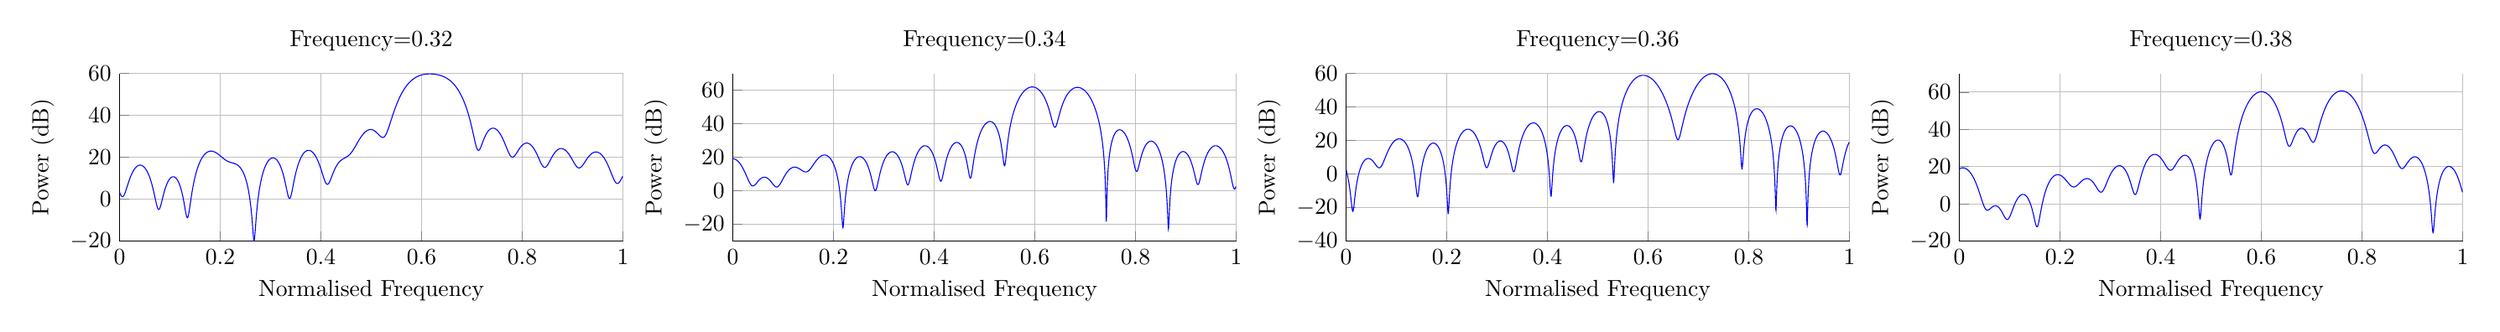
\begin{tikzpicture}

\begin{axis}[%
width=3in,
height=1in,
scale only axis,
xmin=0,
xmax=1,
xlabel={Normalised Frequency},
xmajorgrids,
ymin=-30,
ymax=70,
ylabel={Power (dB)},
ymajorgrids,
name=plot2,
title={Frequency=0.34},
axis x line*=bottom,
axis y line*=left
]
\addplot [color=blue,solid,forget plot]
  table[row sep=crcr]{-1	3.21515738155582\\
-0.99951171875	3.78047725883954\\
-0.9990234375	4.37210663327919\\
-0.99853515625	4.98056218751298\\
-0.998046875	5.59787469531732\\
-0.99755859375	6.21750880349247\\
-0.9970703125	6.83421857337718\\
-0.99658203125	7.44387555796662\\
-0.99609375	8.04329367507241\\
-0.99560546875	8.6300651124274\\
-0.9951171875	9.20241435718551\\
-0.99462890625	9.7590728070382\\
-0.994140625	10.2991736781446\\
-0.99365234375	10.8221654825816\\
-0.9931640625	11.3277417318546\\
-0.99267578125	11.8157843945222\\
-0.9921875	12.2863187703776\\
-0.99169921875	12.7394777006145\\
-0.9912109375	13.175473330645\\
-0.99072265625	13.5945749347593\\
-0.990234375	13.997091577652\\
-0.98974609375	14.3833586184063\\
-0.9892578125	14.7537272566388\\
-0.98876953125	15.1085564806889\\
-0.98828125	15.4482069080964\\
-0.98779296875	15.7730361136839\\
-0.9873046875	16.0833951246555\\
-0.98681640625	16.3796258291281\\
-0.986328125	16.6620590976999\\
-0.98583984375	16.9310134598056\\
-0.9853515625	17.1867942099419\\
-0.98486328125	17.4296928452012\\
-0.984375	17.659986756369\\
-0.98388671875	17.8779391112904\\
-0.9833984375	18.0837988822057\\
-0.98291015625	18.2778009790238\\
-0.982421875	18.4601664586169\\
-0.98193359375	18.6311027866304\\
-0.9814453125	18.7908041333719\\
-0.98095703125	18.9394516893422\\
-0.98046875	19.0772139891283\\
-0.97998046875	19.2042472348696\\
-0.9794921875	19.3206956124583\\
-0.97900390625	19.4266915951745\\
-0.978515625	19.5223562306472\\
-0.97802734375	19.6077994079597\\
-0.9775390625	19.6831201024303\\
-0.97705078125	19.7484065961334\\
-0.9765625	19.8037366726281\\
-0.97607421875	19.8491777846416\\
-0.9755859375	19.8847871936529\\
-0.97509765625	19.9106120804323\\
-0.974609375	19.9266896256514\\
-0.97412109375	19.9330470596741\\
-0.9736328125	19.9297016805921\\
-0.97314453125	19.9166608394816\\
-0.97265625	19.8939218917301\\
-0.97216796875	19.8614721131191\\
-0.9716796875	19.8192885791542\\
-0.97119140625	19.7673380058983\\
-0.970703125	19.7055765502963\\
-0.97021484375	19.6339495676696\\
-0.9697265625	19.5523913237074\\
-0.96923828125	19.4608246578819\\
-0.96875	19.3591605947591\\
-0.96826171875	19.2472978991644\\
-0.9677734375	19.1251225705736\\
-0.96728515625	18.9925072714333\\
-0.966796875	18.8493106833547\\
-0.96630859375	18.6953767842496\\
-0.9658203125	18.5305340384783\\
-0.96533203125	18.3545944909274\\
-0.96484375	18.1673527546008\\
-0.96435546875	17.9685848797719\\
-0.9638671875	17.7580470909454\\
-0.96337890625	17.5354743757957\\
-0.962890625	17.3005789078003\\
-0.96240234375	17.0530482814212\\
-0.9619140625	16.7925435353078\\
-0.96142578125	16.5186969350021\\
-0.9609375	16.2311094818892\\
-0.96044921875	15.9293481094949\\
-0.9599609375	15.6129425214836\\
-0.95947265625	15.2813816176155\\
-0.958984375	14.9341094441558\\
-0.95849609375	14.5705205934089\\
-0.9580078125	14.1899549626725\\
-0.95751953125	13.7916917653327\\
-0.95703125	13.3749426652349\\
-0.95654296875	12.9388438788202\\
-0.9560546875	12.4824470564339\\
-0.95556640625	12.0047087129162\\
-0.955078125	11.5044779257247\\
-0.95458984375	10.9804819532995\\
-0.9541015625	10.4313093430246\\
-0.95361328125	9.85538999139238\\
-0.953125	9.25097148128807\\
-0.95263671875	8.61609084239741\\
-0.9521484375	7.94854064642676\\
-0.95166015625	7.24582803947529\\
-0.951171875	6.50512490204434\\
-0.95068359375	5.72320677411714\\
-0.9501953125	4.89637743358561\\
-0.94970703125	4.02037499268245\\
-0.94921875	3.0902539667664\\
-0.94873046875	2.10023581214341\\
-0.9482421875	1.04351769636102\\
-0.94775390625	-0.0879745615738002\\
-0.947265625	-1.30390878049658\\
-0.94677734375	-2.61597066489848\\
-0.9462890625	-4.03842639485245\\
-0.94580078125	-5.58887133198598\\
-0.9453125	-7.28922172392885\\
-0.94482421875	-9.16699775503867\\
-0.9443359375	-11.2568681823145\\
-0.94384765625	-13.6021079547498\\
-0.943359375	-16.2544900209191\\
-0.94287109375	-19.2672511462683\\
-0.9423828125	-22.6626437433892\\
-0.94189453125	-26.3153548936798\\
-0.94140625	-29.6269432732307\\
-0.94091796875	-31.1751936369899\\
-0.9404296875	-29.862413998356\\
-0.93994140625	-26.6559451296282\\
-0.939453125	-23.0264803993769\\
-0.93896484375	-19.6305265983446\\
-0.9384765625	-16.6152238068739\\
-0.93798828125	-13.9639115482997\\
-0.9375	-11.6240458044163\\
-0.93701171875	-9.54331994892719\\
-0.9365234375	-7.67774220631153\\
-0.93603515625	-5.99200906465965\\
-0.935546875	-4.45809225418014\\
-0.93505859375	-3.05368108989602\\
-0.9345703125	-1.76087581037901\\
-0.93408203125	-0.565174314846809\\
-0.93359375	0.545293555734458\\
-0.93310546875	1.58034138599688\\
-0.9326171875	2.54815987225948\\
-0.93212890625	3.45564606550595\\
-0.931640625	4.30865557489922\\
-0.93115234375	5.11219763002042\\
-0.9306640625	5.87058742379749\\
-0.93017578125	6.58756622956038\\
-0.9296875	7.26639697915518\\
-0.92919921875	7.90994097960606\\
-0.9287109375	8.52071999897551\\
-0.92822265625	9.10096690259959\\
-0.927734375	9.6526672533119\\
-0.92724609375	10.1775937230197\\
-0.9267578125	10.6773347416001\\
-0.92626953125	11.1533184927793\\
-0.92578125	11.6068331272351\\
-0.92529296875	12.0390438804562\\
-0.9248046875	12.4510076423755\\
-0.92431640625	12.8436854169137\\
-0.923828125	13.2179530245935\\
-0.92333984375	13.5746103346135\\
-0.9228515625	13.9143892599527\\
-0.92236328125	14.2379607070466\\
-0.921875	14.5459406379182\\
-0.92138671875	14.8388953755441\\
-0.9208984375	15.1173462613023\\
-0.92041015625	15.3817737554828\\
-0.919921875	15.632621057247\\
-0.91943359375	15.8702973084103\\
-0.9189453125	16.0951804355219\\
-0.91845703125	16.3076196764924\\
-0.91796875	16.507937831182\\
-0.91748046875	16.6964332696369\\
-0.9169921875	16.8733817268634\\
-0.91650390625	17.0390379089769\\
-0.916015625	17.1936369321429\\
-0.91552734375	17.3373956128203\\
-0.9150390625	17.4705136253395\\
-0.91455078125	17.5931745407338\\
-0.9140625	17.7055467589226\\
-0.91357421875	17.8077843447842\\
-0.9130859375	17.9000277773012\\
-0.91259765625	17.982404619791\\
-0.912109375	18.055030118213\\
-0.91162109375	18.1180077336517\\
-0.9111328125	18.1714296142911\\
-0.91064453125	18.2153770115057\\
-0.91015625	18.2499206440838\\
-0.90966796875	18.2751210140497\\
-0.9091796875	18.2910286770678\\
-0.90869140625	18.2976844699693\\
-0.908203125	18.2951196975432\\
-0.90771484375	18.2833562803703\\
-0.9072265625	18.2624068651399\\
-0.90673828125	18.2322748985763\\
-0.90625	18.192954665812\\
-0.90576171875	18.1444312937585\\
-0.9052734375	18.0866807197663\\
-0.90478515625	18.0196696256013\\
-0.904296875	17.9433553365141\\
-0.90380859375	17.8576856849264\\
-0.9033203125	17.7625988380119\\
-0.90283203125	17.6580230881922\\
-0.90234375	17.5438766053171\\
-0.90185546875	17.4200671490328\\
-0.9013671875	17.2864917395766\\
-0.90087890625	17.1430362849559\\
-0.900390625	16.9895751621855\\
-0.89990234375	16.8259707499583\\
-0.8994140625	16.6520729098234\\
-0.89892578125	16.4677184126286\\
-0.8984375	16.2727303066716\\
-0.89794921875	16.0669172236845\\
-0.8974609375	15.850072618469\\
-0.89697265625	15.6219739377082\\
-0.896484375	15.3823817132224\\
-0.89599609375	15.1310385747372\\
-0.8955078125	14.8676681771117\\
-0.89501953125	14.5919740369876\\
-0.89453125	14.3036382740103\\
-0.89404296875	14.0023202522289\\
-0.8935546875	13.6876551181046\\
-0.89306640625	13.3592522328877\\
-0.892578125	13.0166934991674\\
-0.89208984375	12.6595315844151\\
-0.8916015625	12.2872880486998\\
-0.89111328125	11.8994513899519\\
-0.890625	11.4954750288668\\
-0.89013671875	11.0747752676998\\
-0.8896484375	10.636729274098\\
-0.88916015625	10.1806731644714\\
-0.888671875	9.7059002936741\\
-0.88818359375	9.21165990223884\\
-0.8876953125	8.69715633372897\\
-0.88720703125	8.16154911928786\\
-0.88671875	7.60395434302703\\
-0.88623046875	7.02344786272897\\
-0.8857421875	6.41907118236711\\
-0.88525390625	5.78984107947563\\
-0.884765625	5.13476451334348\\
-0.88427734375	4.45286092255021\\
-0.8837890625	3.74319481992367\\
-0.88330078125	3.00492268365238\\
-0.8828125	2.23735961579512\\
-0.88232421875	1.44007319470218\\
-0.8818359375	0.61301447499998\\
-0.88134765625	-0.243300789425176\\
-0.880859375	-1.12754407019562\\
-0.88037109375	-2.03723910830066\\
-0.8798828125	-2.96831825412632\\
-0.87939453125	-3.91455114362419\\
-0.87890625	-4.86683997364143\\
-0.87841796875	-5.8124086037463\\
-0.8779296875	-6.73397816659963\\
-0.87744140625	-7.60913101320766\\
-0.876953125	-8.41021224354887\\
-0.87646484375	-9.1052528900849\\
-0.8759765625	-9.66039506770967\\
-0.87548828125	-10.0439776543235\\
-0.875	-10.2317166818127\\
-0.87451171875	-10.2115425112543\\
-0.8740234375	-9.98627698966759\\
-0.87353515625	-9.57299114325332\\
-0.873046875	-8.99933058401892\\
-0.87255859375	-8.29833966596197\\
-0.8720703125	-7.50356362262604\\
-0.87158203125	-6.645560424787\\
-0.87109375	-5.75007829162875\\
-0.87060546875	-4.83757342574646\\
-0.8701171875	-3.92355889317101\\
-0.86962890625	-3.0193430245304\\
-0.869140625	-2.13286550895047\\
-0.86865234375	-1.26947529991157\\
-0.8681640625	-0.432586621337915\\
-0.86767578125	0.37579884042518\\
-0.8671875	1.15469119174591\\
-0.86669921875	1.90381217605471\\
-0.8662109375	2.62337411598631\\
-0.86572265625	3.31391910353916\\
-0.865234375	3.97620315594255\\
-0.86474609375	4.61111348699183\\
-0.8642578125	5.21960994988521\\
-0.86376953125	5.80268401430248\\
-0.86328125	6.36133040457366\\
-0.86279296875	6.89652784489935\\
-0.8623046875	7.40922633031877\\
-0.86181640625	7.90033905332243\\
-0.861328125	8.37073763336387\\
-0.86083984375	8.82124967183332\\
-0.8603515625	9.25265792697503\\
-0.85986328125	9.66570060018186\\
-0.859375	10.0610723677921\\
-0.85888671875	10.4394258959478\\
-0.8583984375	10.8013736510874\\
-0.85791015625	11.1474898730734\\
-0.857421875	11.4783126174325\\
-0.85693359375	11.7943458018138\\
-0.8564453125	12.096061212485\\
-0.85595703125	12.3839004416496\\
-0.85546875	12.6582767371229\\
-0.85498046875	12.9195767535949\\
-0.8544921875	13.1681622001571\\
-0.85400390625	13.4043713825832\\
-0.853515625	13.6285206414792\\
-0.85302734375	13.8409056891719\\
-0.8525390625	14.0418028493356\\
-0.85205078125	14.2314702040333\\
-0.8515625	14.4101486532015\\
-0.85107421875	14.5780628917322\\
-0.8505859375	14.7354223092728\\
-0.85009765625	14.8824218177168\\
-0.849609375	15.0192426111474\\
-0.84912109375	15.1460528627308\\
-0.8486328125	15.2630083627728\\
-0.84814453125	15.3702531018491\\
-0.84765625	15.4679198026209\\
-0.84716796875	15.5561304036448\\
-0.8466796875	15.6349964981973\\
-0.84619140625	15.7046197308503\\
-0.845703125	15.7650921542677\\
-0.84521484375	15.8164965484302\\
-0.8447265625	15.8589067042565\\
-0.84423828125	15.8923876733479\\
-0.84375	15.916995985365\\
-0.84326171875	15.9327798343268\\
-0.8427734375	15.9397792349184\\
-0.84228515625	15.938026149694\\
-0.841796875	15.9275445878635\\
-0.84130859375	15.9083506761661\\
-0.8408203125	15.8804527021389\\
-0.84033203125	15.8438511299029\\
-0.83984375	15.7985385883958\\
-0.83935546875	15.7444998317863\\
-0.8388671875	15.6817116716032\\
-0.83837890625	15.6101428799024\\
-0.837890625	15.5297540625738\\
-0.83740234375	15.4404975016567\\
-0.8369140625	15.3423169652771\\
-0.83642578125	15.2351474835525\\
-0.8359375	15.1189150885074\\
-0.83544921875	14.99353651572\\
-0.8349609375	14.8589188650584\\
-0.83447265625	14.7149592174629\\
-0.833984375	14.5615442042815\\
-0.83349609375	14.3985495251643\\
-0.8330078125	14.225839409947\\
-0.83251953125	14.0432660193141\\
-0.83203125	13.8506687782905\\
-0.83154296875	13.6478736357748\\
-0.8310546875	13.4346922423574\\
-0.83056640625	13.2109210375599\\
-0.830078125	12.9763402363487\\
-0.82958984375	12.7307127032845\\
-0.8291015625	12.4737827009462\\
-0.82861328125	12.2052744972413\\
-0.828125	11.9248908138572\\
-0.82763671875	11.6323110953243\\
-0.8271484375	11.3271895748859\\
-0.82666015625	11.0091531094919\\
-0.826171875	10.6777987516193\\
-0.82568359375	10.3326910201246\\
-0.8251953125	9.97335882574437\\
-0.82470703125	9.59929199893182\\
-0.82421875	9.20993735814094\\
-0.82373046875	8.80469424504232\\
-0.8232421875	8.38290943897036\\
-0.82275390625	7.94387134551181\\
-0.822265625	7.4868033327084\\
-0.82177734375	7.01085606177376\\
-0.8212890625	6.51509862608734\\
-0.82080078125	5.99850827064793\\
-0.8203125	5.45995841164531\\
-0.81982421875	4.89820460899539\\
-0.8193359375	4.31186805905701\\
-0.81884765625	3.69941606413986\\
-0.818359375	3.05913879131805\\
-0.81787109375	2.38912144365257\\
-0.8173828125	1.68721071552488\\
-0.81689453125	0.950974066646524\\
-0.81640625	0.177649892126594\\
-0.81591796875	-0.635913961463861\\
-0.8154296875	-1.49333675645002\\
-0.81494140625	-2.3988011533035\\
-0.814453125	-3.35717564241372\\
-0.81396484375	-4.37417209609451\\
-0.8134765625	-5.45655122063207\\
-0.81298828125	-6.61239444083168\\
-0.8125	-7.85146964952246\\
-0.81201171875	-9.18573236864166\\
-0.8115234375	-10.6300268777635\\
-0.81103515625	-12.2030905538202\\
-0.810546875	-13.9290320181039\\
-0.81005859375	-15.839575633783\\
-0.8095703125	-17.9775956803302\\
-0.80908203125	-20.4029224140609\\
-0.80859375	-23.2023647405864\\
-0.80810546875	-26.5080197307243\\
-0.8076171875	-30.5327450660499\\
-0.80712890625	-35.6409815414898\\
-0.806640625	-42.4589212358848\\
-0.80615234375	-51.3179159761684\\
-0.8056640625	-54.0564312324987\\
-0.80517578125	-45.6154492509258\\
-0.8046875	-38.1407778179806\\
-0.80419921875	-32.6455822863445\\
-0.8037109375	-28.4220373809787\\
-0.80322265625	-25.0246666630373\\
-0.802734375	-22.1973913528769\\
-0.80224609375	-19.7847723480616\\
-0.8017578125	-17.6866180330392\\
-0.80126953125	-15.8349642343202\\
-0.80078125	-14.181738351843\\
-0.80029296875	-12.691750662109\\
-0.7998046875	-11.3384990415421\\
-0.79931640625	-10.101542532529\\
-0.798828125	-8.96479277154464\\
-0.79833984375	-7.91536530068353\\
-0.7978515625	-6.9427849962884\\
-0.79736328125	-6.0384226523859\\
-0.796875	-5.19508668590276\\
-0.79638671875	-4.40672151103062\\
-0.7958984375	-3.66818086996123\\
-0.79541015625	-2.97505486340553\\
-0.794921875	-2.32353612558461\\
-0.79443359375	-1.71031498358803\\
-0.7939453125	-1.13249638452093\\
-0.79345703125	-0.587533382884296\\
-0.79296875	-0.0731733756949485\\
-0.79248046875	0.412585743004669\\
-0.7919921875	0.871531632206988\\
-0.79150390625	1.30526737160949\\
-0.791015625	1.7152363847422\\
-0.79052734375	2.10274337672793\\
-0.7900390625	2.46897203665838\\
-0.78955078125	2.81500009598028\\
-0.7890625	3.14181221294811\\
-0.78857421875	3.45031105955961\\
-0.7880859375	3.7413269145428\\
-0.78759765625	4.01562600885644\\
-0.787109375	4.27391782508216\\
-0.78662109375	4.51686151624919\\
-0.7861328125	4.74507158096501\\
-0.78564453125	4.95912290864814\\
-0.78515625	5.15955528997529\\
-0.78466796875	5.34687747243538\\
-0.7841796875	5.52157082841504\\
-0.78369140625	5.68409269296469\\
-0.783203125	5.83487941986974\\
-0.78271484375	5.97434919753464\\
-0.7822265625	6.10290466019246\\
-0.78173828125	6.22093532486518\\
-0.78125	6.32881988012736\\
-0.78076171875	6.42692834892541\\
-0.7802734375	6.51562414434782\\
-0.77978515625	6.59526603422507\\
-0.779296875	6.66621002766921\\
-0.77880859375	6.72881119406891\\
-0.7783203125	6.78342542256529\\
-0.77783203125	6.8304111275891\\
-0.77734375	6.87013090359057\\
-0.77685546875	6.9029531295931\\
-0.7763671875	6.92925352161423\\
-0.77587890625	6.94941662829116\\
-0.775390625	6.96383726220606\\
-0.77490234375	6.97292185641235\\
-0.7744140625	6.97708973252734\\
-0.77392578125	6.97677426349154\\
-0.7734375	6.97242391074279\\
-0.77294921875	6.96450311217226\\
-0.7724609375	6.95349299390643\\
-0.77197265625	6.93989187580902\\
-0.771484375	6.92421553776909\\
-0.77099609375	6.90699721151333\\
-0.7705078125	6.88878726106864\\
-0.77001953125	6.87015251434573\\
-0.76953125	6.85167520888277\\
-0.76904296875	6.83395151685653\\
-0.7685546875	6.81758961831366\\
-0.76806640625	6.80320729744267\\
-0.767578125	6.79142904480213\\
-0.76708984375	6.78288265885694\\
-0.7666015625	6.77819535296313\\
-0.76611328125	6.7779893889405\\
-0.765625	6.78287727527101\\
-0.76513671875	6.79345658625247\\
-0.7646484375	6.81030447741418\\
-0.76416015625	6.83397199126725\\
-0.763671875	6.86497826496164\\
-0.76318359375	6.90380476649606\\
-0.7626953125	6.95088969759827\\
-0.76220703125	7.00662270814719\\
-0.76171875	7.07134006812018\\
-0.76123046875	7.1453204378711\\
-0.7607421875	7.22878136580627\\
-0.76025390625	7.32187662440186\\
-0.759765625	7.42469447163013\\
-0.75927734375	7.53725689632042\\
-0.7587890625	7.65951987423098\\
-0.75830078125	7.79137462837903\\
-0.7578125	7.93264985432037\\
-0.75732421875	8.08311484040683\\
-0.7568359375	8.24248338621697\\
-0.75634765625	8.41041840067466\\
-0.755859375	8.58653704574984\\
-0.75537109375	8.77041628253254\\
-0.7548828125	8.961598673869\\
-0.75439453125	9.15959830122631\\
-0.75390625	9.36390666223275\\
-0.75341796875	9.57399842841447\\
-0.7529296875	9.78933695886474\\
-0.75244140625	10.009379483757\\
-0.751953125	10.2335818906233\\
-0.75146484375	10.4614030651688\\
-0.7509765625	10.6923087562575\\
-0.75048828125	10.9257749509531\\
-0.75	11.1612907597149\\
-0.74951171875	11.39836082378\\
-0.7490234375	11.6365072663476\\
-0.74853515625	11.8752712164583\\
-0.748046875	12.1142139396089\\
-0.74755859375	12.3529176123614\\
-0.7470703125	12.5909857797816\\
-0.74658203125	12.8280435347345\\
-0.74609375	13.0637374571728\\
-0.74560546875	13.2977353498117\\
-0.7451171875	13.5297258042556\\
-0.74462890625	13.7594176289004\\
-0.744140625	13.9865391669819\\
-0.74365234375	14.210837530087\\
-0.7431640625	14.4320777694254\\
-0.74267578125	14.6500420042315\\
-0.7421875	14.8645285239128\\
-0.74169921875	15.0753508779989\\
-0.7412109375	15.2823369656141\\
-0.74072265625	15.485328134096\\
-0.740234375	15.6841782945159\\
-0.73974609375	15.8787530602188\\
-0.7392578125	16.0689289130794\\
-0.73876953125	16.2545924009442\\
-0.73828125	16.4356393686928\\
-0.73779296875	16.6119742244741\\
-0.7373046875	16.7835092419476\\
-0.73681640625	16.9501638987581\\
-0.736328125	17.1118642509918\\
-0.73583984375	17.2685423429681\\
-0.7353515625	17.4201356514257\\
-0.73486328125	17.5665865629205\\
-0.734375	17.7078418830893\\
-0.73388671875	17.8438523763045\\
-0.7333984375	17.9745723341672\\
-0.73291015625	18.09995917124\\
-0.732421875	18.2199730463989\\
-0.73193359375	18.3345765081881\\
-0.7314453125	18.44373416258\\
-0.73095703125	18.5474123615755\\
-0.73046875	18.6455789111227\\
-0.72998046875	18.7382027968801\\
-0.7294921875	18.8252539264071\\
-0.72900390625	18.9067028864181\\
-0.728515625	18.9825207137986\\
-0.72802734375	19.0526786791381\\
-0.7275390625	19.1171480815916\\
-0.72705078125	19.1759000539392\\
-0.7265625	19.2289053767653\\
-0.72607421875	19.2761343007312\\
-0.7255859375	19.3175563759608\\
-0.72509765625	19.3531402876045\\
-0.724609375	19.3828536966879\\
-0.72412109375	19.4066630853874\\
-0.7236328125	19.4245336059091\\
-0.72314453125	19.4364289321772\\
-0.72265625	19.4423111135633\\
-0.72216796875	19.44214042991\\
-0.7216796875	19.4358752471211\\
-0.72119140625	19.4234718726043\\
-0.720703125	19.4048844098631\\
-0.72021484375	19.3800646115424\\
-0.7197265625	19.3489617302339\\
-0.71923828125	19.3115223663495\\
-0.71875	19.2676903123632\\
-0.71826171875	19.2174063927194\\
-0.7177734375	19.160608298689\\
-0.71728515625	19.0972304174436\\
-0.716796875	19.027203654599\\
-0.71630859375	18.9504552494565\\
-0.7158203125	18.866908582146\\
-0.71533203125	18.7764829718483\\
-0.71484375	18.6790934652396\\
-0.71435546875	18.5746506142695\\
-0.7138671875	18.4630602423468\\
-0.71337890625	18.3442231979681\\
-0.712890625	18.2180350947849\\
-0.71240234375	18.0843860370632\\
-0.7119140625	17.9431603294519\\
-0.71142578125	17.7942361699352\\
-0.7109375	17.6374853248114\\
-0.71044921875	17.4727727845116\\
-0.7099609375	17.2999563990536\\
-0.70947265625	17.1188864919183\\
-0.708984375	16.929405451151\\
-0.70849609375	16.7313472965244\\
-0.7080078125	16.5245372216753\\
-0.70751953125	16.3087911102371\\
-0.70703125	16.0839150251674\\
-0.70654296875	15.8497046707196\\
-0.7060546875	15.6059448268533\\
-0.70556640625	15.352408756357\\
-0.705078125	15.0888575856\\
-0.70458984375	14.8150396606826\\
-0.7041015625	14.5306898818891\\
-0.70361328125	14.2355290208306\\
-0.703125	13.9292630266094\\
-0.70263671875	13.611582329864\\
-0.7021484375	13.2821611568435\\
-0.70166015625	12.9406568699212\\
-0.701171875	12.5867093564799\\
-0.70068359375	12.2199404952487\\
-0.7001953125	11.8399537384197\\
-0.69970703125	11.4463338598384\\
-0.69921875	11.038646935048\\
-0.69873046875	10.6164406390144\\
-0.6982421875	10.1792449733194\\
-0.69775390625	9.72657356824465\\
-0.697265625	9.25792574874539\\
-0.69677734375	8.77278960978753\\
-0.6962890625	8.27064641965597\\
-0.69580078125	7.75097676447527\\
-0.6953125	7.21326896939091\\
-0.69482421875	6.65703048920686\\
-0.6943359375	6.08180316291006\\
-0.69384765625	5.48718348310342\\
-0.693359375	4.87284935454439\\
-0.69287109375	4.23859521689617\\
-0.6923828125	3.58437789299875\\
-0.69189453125	2.91037609336655\\
-0.69140625	2.21706713741455\\
-0.69091796875	1.50532507944411\\
-0.6904296875	0.776544918583775\\
-0.68994140625	0.0327976721176284\\
-0.689453125	-0.722979644287959\\
-0.68896484375	-1.48675738169706\\
-0.6884765625	-2.2531531594289\\
-0.68798828125	-3.01515052338994\\
-0.6875	-3.76382328816257\\
-0.68701171875	-4.48811387964714\\
-0.6865234375	-5.17474094453452\\
-0.68603515625	-5.80833823936666\\
-0.685546875	-6.3719402356978\\
-0.68505859375	-6.84790918693908\\
-0.6845703125	-7.2193218387331\\
-0.68408203125	-7.47169596377585\\
-0.68359375	-7.59477008060635\\
-0.68310546875	-7.58393098290684\\
-0.6826171875	-7.44090062316143\\
-0.68212890625	-7.17347804873508\\
-0.681640625	-6.79441439933282\\
-0.68115234375	-6.31974308478519\\
-0.6806640625	-5.76698356027484\\
-0.68017578125	-5.15357209933102\\
-0.6796875	-4.49571690203457\\
-0.67919921875	-3.80771654722201\\
-0.6787109375	-3.10167460227779\\
-0.67822265625	-2.38749885952316\\
-0.677734375	-1.67307419628913\\
-0.67724609375	-0.964520772077357\\
-0.6767578125	-0.266477240201434\\
-0.67626953125	0.417627029120902\\
-0.67578125	1.08532895688293\\
-0.67529296875	1.73492476361533\\
-0.6748046875	2.36529911012631\\
-0.67431640625	2.9757871404806\\
-0.673828125	3.56606484850301\\
-0.67333984375	4.1360629718929\\
-0.6728515625	4.68589996935571\\
-0.67236328125	5.21583022308749\\
-0.671875	5.72620424890709\\
-0.67138671875	6.21743829840138\\
-0.6708984375	6.68999126339075\\
-0.67041015625	7.14434723291435\\
-0.669921875	7.58100241086646\\
-0.66943359375	8.00045538839516\\
-0.6689453125	8.40319999087027\\
-0.66845703125	8.78972009586069\\
-0.66796875	9.1604859560129\\
-0.66748046875	9.51595166728931\\
-0.6669921875	9.8565535054466\\
-0.66650390625	10.1827089172945\\
-0.666015625	10.4948160024124\\
-0.66552734375	10.7932533589159\\
-0.6650390625	11.0783801961315\\
-0.66455078125	11.3505366396221\\
-0.6640625	11.6100441714567\\
-0.66357421875	11.8572061620868\\
-0.6630859375	12.0923084606094\\
-0.66259765625	12.3156200182358\\
-0.662109375	12.5273935259987\\
-0.66162109375	12.727866052527\\
-0.6611328125	12.9172596714084\\
-0.66064453125	13.0957820705079\\
-0.66015625	13.2636271377855\\
-0.65966796875	13.4209755198273\\
-0.6591796875	13.5679951505673\\
-0.65869140625	13.7048417486334\\
-0.658203125	13.8316592824649\\
-0.65771484375	13.948580402872\\
-0.6572265625	14.055726843089\\
-0.65673828125	14.153209786636\\
-0.65625	14.2411302034813\\
-0.65576171875	14.3195791551054\\
-0.6552734375	14.3886380691217\\
-0.65478515625	14.4483789841243\\
-0.654296875	14.4988647654145\\
-0.65380859375	14.5401492922145\\
-0.6533203125	14.5722776169167\\
-0.65283203125	14.595286096838\\
-0.65234375	14.6092024988608\\
-0.65185546875	14.6140460772426\\
-0.6513671875	14.6098276247712\\
-0.65087890625	14.596549497327\\
-0.650390625	14.5742056117957\\
-0.64990234375	14.5427814171491\\
-0.6494140625	14.5022538383819\\
-0.64892578125	14.4525911928561\\
-0.6484375	14.3937530784632\\
-0.64794921875	14.325690232868\\
-0.6474609375	14.2483443629467\\
-0.64697265625	14.1616479433707\\
-0.646484375	14.0655239831264\\
-0.64599609375	13.9598857585886\\
-0.6455078125	13.844636511591\\
-0.64501953125	13.7196691107559\\
-0.64453125	13.5848656741611\\
-0.64404296875	13.4400971512349\\
-0.6435546875	13.2852228615869\\
-0.64306640625	13.1200899882992\\
-0.642578125	12.9445330230341\\
-0.64208984375	12.7583731601637\\
-0.6416015625	12.5614176370013\\
-0.64111328125	12.3534590171401\\
-0.640625	12.1342744138845\\
-0.64013671875	11.9036246508375\\
-0.6396484375	11.6612533569041\\
-0.63916015625	11.4068859933463\\
-0.638671875	11.1402288111275\\
-0.63818359375	10.860967737718\\
-0.6376953125	10.5687671938866\\
-0.63720703125	10.2632688429473\\
-0.63671875	9.94409027765154\\
-0.63623046875	9.61082365368338\\
-0.6357421875	9.26303428389258\\
-0.63525390625	8.90025921445309\\
-0.634765625	8.52200581371807\\
-0.63427734375	8.12775041750903\\
-0.6337890625	7.71693709209622\\
-0.63330078125	7.28897659976546\\
-0.6328125	6.84324568374681\\
-0.63232421875	6.37908683227522\\
-0.6318359375	5.8958087395511\\
-0.63134765625	5.39268775964775\\
-0.630859375	4.86897075510464\\
-0.63037109375	4.3238798847043\\
-0.6298828125	3.75662006773178\\
-0.62939453125	3.16639012220745\\
-0.62890625	2.55239892510146\\
-0.62841796875	1.91388841316489\\
-0.6279296875	1.25016587139267\\
-0.62744140625	0.56064878767166\\
-0.626953125	-0.155073362760884\\
-0.62646484375	-0.897154654291331\\
-0.6259765625	-1.66537811370128\\
-0.62548828125	-2.45900155191248\\
-0.625	-3.27655233522326\\
-0.62451171875	-4.11555799768542\\
-0.6240234375	-4.97219952358918\\
-0.62353515625	-5.84087766266546\\
-0.623046875	-6.71369332730543\\
-0.62255859375	-7.57986633454662\\
-0.6220703125	-8.42515916709333\\
-0.62158203125	-9.23143903363045\\
-0.62109375	-9.97659790254373\\
-0.62060546875	-10.6351289692799\\
-0.6201171875	-11.1796653609972\\
-0.61962890625	-11.5836304352097\\
-0.619140625	-11.8247690193163\\
-0.61865234375	-11.8888105598642\\
-0.6181640625	-11.7721498273803\\
-0.61767578125	-11.4825649488501\\
-0.6171875	-11.0376898286786\\
-0.61669921875	-10.4618329226357\\
-0.6162109375	-9.78224474490757\\
-0.61572265625	-9.02585487347931\\
-0.615234375	-8.21703308197472\\
-0.61474609375	-7.37643878390009\\
-0.6142578125	-6.52072648075301\\
-0.61376953125	-5.66279017241423\\
-0.61328125	-4.81227349772603\\
-0.61279296875	-3.9761593086051\\
-0.6123046875	-3.15933304079126\\
-0.61181640625	-2.36507163000607\\
-0.611328125	-1.59544421601321\\
-0.61083984375	-0.851628693770923\\
-0.6103515625	-0.134155670864949\\
-0.60986328125	0.556906740915819\\
-0.609375	1.22181469502428\\
-0.60888671875	1.86104619913532\\
-0.6083984375	2.47522584728606\\
-0.60791015625	3.06506991086987\\
-0.607421875	3.63134659195463\\
-0.60693359375	4.17484751145834\\
-0.6064453125	4.69636748959944\\
-0.60595703125	5.19669042632103\\
-0.60546875	5.67657965421012\\
-0.60498046875	6.13677155844179\\
-0.6044921875	6.57797157212825\\
-0.60400390625	7.00085188823555\\
-0.603515625	7.40605040165697\\
-0.60302734375	7.79417052268912\\
-0.6025390625	8.16578159767612\\
-0.60205078125	8.52141974260037\\
-0.6015625	8.86158894727924\\
-0.60107421875	9.18676234629159\\
-0.6005859375	9.49738358127661\\
-0.60009765625	9.79386820038858\\
-0.599609375	10.0766050563522\\
-0.59912109375	10.3459576761439\\
-0.5986328125	10.6022655838713\\
-0.59814453125	10.8458455647012\\
-0.59765625	11.0769928622797\\
-0.59716796875	11.2959823054178\\
-0.5966796875	11.5030693622041\\
-0.59619140625	11.6984911213959\\
-0.595703125	11.8824672021052\\
-0.59521484375	12.0552005935714\\
-0.5947265625	12.216878427304\\
-0.59423828125	12.3676726841542\\
-0.59375	12.5077408389956\\
-0.59326171875	12.6372264456995\\
-0.5927734375	12.7562596650159\\
-0.59228515625	12.8649577378372\\
-0.591796875	12.9634254061383\\
-0.59130859375	13.0517552836886\\
-0.5908203125	13.1300281783941\\
-0.59033203125	13.1983133678895\\
-0.58984375	13.2566688297464\\
-0.58935546875	13.3051414273979\\
-0.5888671875	13.3437670526144\\
-0.58837890625	13.3725707250854\\
-0.587890625	13.3915666493813\\
-0.58740234375	13.4007582292726\\
-0.5869140625	13.4001380390829\\
-0.58642578125	13.3896877514329\\
-0.5859375	13.3693780203982\\
-0.58544921875	13.3391683187515\\
-0.5849609375	13.2990067275785\\
-0.58447265625	13.2488296761511\\
-0.583984375	13.1885616294981\\
-0.58349609375	13.1181147206286\\
-0.5830078125	13.0373883238334\\
-0.58251953125	12.9462685648964\\
-0.58203125	12.8446277633949\\
-0.58154296875	12.7323238015286\\
-0.5810546875	12.6091994130951\\
-0.58056640625	12.4750813852902\\
-0.580078125	12.3297796649575\\
-0.57958984375	12.1730863597035\\
-0.5791015625	12.0047746229195\\
-0.57861328125	11.8245974101771\\
-0.578125	11.6322860926522\\
-0.57763671875	11.4275489111506\\
-0.5771484375	11.2100692519035\\
-0.57666015625	10.9795037225173\\
-0.576171875	10.7354800032363\\
-0.57568359375	10.4775944449327\\
-0.5751953125	10.2054093808753\\
-0.57470703125	9.91845011425076\\
-0.57421875	9.61620153748731\\
-0.57373046875	9.2981043325116\\
-0.5732421875	8.96355069299579\\
-0.57275390625	8.61187950022553\\
-0.572265625	8.24237087323216\\
-0.57177734375	7.85424000105652\\
-0.5712890625	7.44663015021738\\
-0.57080078125	7.01860472343144\\
-0.5703125	6.56913822623592\\
-0.56982421875	6.0971059763925\\
-0.5693359375	5.60127236708538\\
-0.56884765625	5.08027746975496\\
-0.568359375	4.53262173761637\\
-0.56787109375	3.95664854975002\\
-0.5673828125	3.35052432402179\\
-0.56689453125	2.71221593545974\\
-0.56640625	2.03946522327395\\
-0.56591796875	1.32976048587703\\
-0.5654296875	0.580305103116048\\
-0.56494140625	-0.212016118401579\\
-0.564453125	-1.05067144653485\\
-0.56396484375	-1.93951464912467\\
-0.5634765625	-2.88280978338937\\
-0.56298828125	-3.88523814483106\\
-0.5625	-4.95186900224903\\
-0.56201171875	-6.08806136105593\\
-0.5615234375	-7.29923865415327\\
-0.56103515625	-8.59043373443584\\
-0.560546875	-9.96542416615328\\
-0.56005859375	-11.4251470683535\\
-0.5595703125	-12.9648758646892\\
-0.55908203125	-14.5693631660027\\
-0.55859375	-16.2049493177938\\
-0.55810546875	-17.8081012555434\\
-0.5576171875	-19.2725762259349\\
-0.55712890625	-20.4447353965214\\
-0.556640625	-21.1462934510813\\
-0.55615234375	-21.2376541299745\\
-0.5556640625	-20.6915968791021\\
-0.55517578125	-19.6098919273197\\
-0.5546875	-18.1648538249512\\
-0.55419921875	-16.524940775333\\
-0.5537109375	-14.8157807117106\\
-0.55322265625	-13.1165447026337\\
-0.552734375	-11.4712562511025\\
-0.55224609375	-9.90135179852823\\
-0.5517578125	-8.41501138517657\\
-0.55126953125	-7.01310827779681\\
-0.55078125	-5.69273322027626\\
-0.55029296875	-4.44919781923983\\
-0.5498046875	-3.27714020453593\\
-0.54931640625	-2.17111629449779\\
-0.548828125	-1.12590116320919\\
-0.54833984375	-0.136629123615707\\
-0.5478515625	0.801154500027642\\
-0.54736328125	1.69148870222374\\
-0.546875	2.53801605951548\\
-0.54638671875	3.34401299784496\\
-0.5458984375	4.11242395440793\\
-0.54541015625	4.84589563244676\\
-0.544921875	5.54680942268782\\
-0.54443359375	6.21731111969287\\
-0.5439453125	6.85933764455983\\
-0.54345703125	7.47464079776861\\
-0.54296875	8.06480822336607\\
-0.54248046875	8.63128183529875\\
-0.5419921875	9.17537397757068\\
-0.54150390625	9.69828158467483\\
-0.541015625	10.2010985904872\\
-0.54052734375	10.684826809971\\
-0.5400390625	11.1503854927542\\
-0.53955078125	11.5986197231258\\
-0.5390625	12.0303078183425\\
-0.53857421875	12.4461678567862\\
-0.5380859375	12.8468634495585\\
-0.53759765625	13.2330088534464\\
-0.537109375	13.6051735096448\\
-0.53662109375	13.9638860809618\\
-0.5361328125	14.3096380502152\\
-0.53564453125	14.6428869339567\\
-0.53515625	14.9640591583093\\
-0.53466796875	15.2735526374195\\
-0.5341796875	15.5717390896384\\
-0.53369140625	15.8589661219309\\
-0.533203125	16.13555910905\\
-0.53271484375	16.40182289061\\
-0.5322265625	16.6580433062627\\
-0.53173828125	16.9044885866569\\
-0.53125	17.1414106156791\\
-0.53076171875	17.3690460775904\\
-0.5302734375	17.5876175010373\\
-0.52978515625	17.7973342104975\\
-0.529296875	17.9983931944862\\
-0.52880859375	18.1909798987733\\
-0.5283203125	18.3752689519237\\
-0.52783203125	18.5514248296479\\
-0.52734375	18.7196024637354\\
-0.52685546875	18.8799478007064\\
-0.5263671875	19.0325983147632\\
-0.52587890625	19.1776834791329\\
-0.525390625	19.3153251994588\\
-0.52490234375	19.4456382125155\\
-0.5244140625	19.5687304531847\\
-0.52392578125	19.6847033923241\\
-0.5234375	19.7936523478975\\
-0.52294921875	19.8956667714923\\
-0.5224609375	19.9908305121392\\
-0.52197265625	20.0792220591565\\
-0.521484375	20.1609147655704\\
-0.52099609375	20.2359770535108\\
-0.5205078125	20.3044726028397\\
-0.52001953125	20.366460524148\\
-0.51953125	20.4219955171419\\
-0.51904296875	20.4711280153349\\
-0.5185546875	20.5139043178734\\
-0.51806640625	20.5503667092332\\
-0.517578125	20.5805535674483\\
-0.51708984375	20.6044994614629\\
-0.5166015625	20.6222352381279\\
-0.51611328125	20.6337880993055\\
-0.515625	20.6391816694841\\
-0.51513671875	20.6384360542564\\
-0.5146484375	20.63156788996\\
-0.51416015625	20.6185903847319\\
-0.513671875	20.5995133511857\\
-0.51318359375	20.5743432308728\\
-0.5126953125	20.5430831106476\\
-0.51220703125	20.5057327310168\\
-0.51171875	20.4622884865092\\
-0.51123046875	20.4127434180646\\
-0.5107421875	20.3570871973965\\
-0.51025390625	20.2953061032473\\
-0.509765625	20.2273829894061\\
-0.50927734375	20.1532972443228\\
-0.5087890625	20.0730247421039\\
-0.50830078125	19.9865377846299\\
-0.5078125	19.8938050344857\\
-0.50732421875	19.7947914383439\\
-0.5068359375	19.6894581403864\\
-0.50634765625	19.5777623852899\\
-0.505859375	19.4596574102387\\
-0.50537109375	19.3350923253598\\
-0.5048828125	19.2040119819015\\
-0.50439453125	19.0663568273942\\
-0.50390625	18.9220627469464\\
-0.50341796875	18.7710608897297\\
-0.5029296875	18.6132774796001\\
-0.50244140625	18.4486336086853\\
-0.501953125	18.2770450126373\\
-0.50146484375	18.0984218261024\\
-0.5009765625	17.9126683168009\\
-0.50048828125	17.7196825964282\\
-0.5	17.5193563063861\\
-0.49951171875	17.3115742761287\\
-0.4990234375	17.0962141516512\\
-0.49853515625	16.8731459913673\\
-0.498046875	16.6422318262949\\
-0.49755859375	16.4033251811103\\
-0.4970703125	16.1562705522139\\
-0.49658203125	15.9009028384861\\
-0.49609375	15.6370467198797\\
-0.49560546875	15.3645159783867\\
-0.4951171875	15.0831127552275\\
-0.49462890625	14.7926267373178\\
-0.494140625	14.4928342651581\\
-0.49365234375	14.1834973532478\\
-0.4931640625	13.8643626129208\\
-0.49267578125	13.5351600661089\\
-0.4921875	13.1956018369299\\
-0.49169921875	12.8453807061259\\
-0.4912109375	12.4841685112051\\
-0.49072265625	12.1116143725989\\
-0.490234375	11.7273427231796\\
-0.48974609375	11.3309511150001\\
-0.4892578125	10.9220077730174\\
-0.48876953125	10.5000488607321\\
-0.48828125	10.0645754169543\\
-0.48779296875	9.61504991612193\\
-0.4873046875	9.15089239652638\\
-0.48681640625	8.67147609115819\\
-0.486328125	8.17612248435577\\
-0.48583984375	7.66409570358832\\
-0.4853515625	7.1345961390339\\
-0.48486328125	6.58675316348794\\
-0.484375	6.01961680078301\\
-0.48388671875	5.43214816136263\\
-0.4833984375	4.82320842776603\\
-0.48291015625	4.19154612912871\\
-0.482421875	3.53578239069879\\
-0.48193359375	2.85439377982634\\
-0.4814453125	2.14569229167563\\
-0.48095703125	1.40780192370135\\
-0.48046875	0.638631175613037\\
-0.47998046875	-0.164159319993289\\
-0.4794921875	-1.00319498056341\\
-0.47900390625	-1.88143237470671\\
-0.478515625	-2.80221249939016\\
-0.47802734375	-3.76932359639344\\
-0.4775390625	-4.78707484331379\\
-0.47705078125	-5.86038192072019\\
-0.4765625	-6.99486447335169\\
-0.47607421875	-8.1969531654916\\
-0.4755859375	-9.47399901526401\\
-0.47509765625	-10.8343672415579\\
-0.474609375	-12.2874764209292\\
-0.47412109375	-13.8436999813794\\
-0.4736328125	-15.5139576434004\\
-0.47314453125	-17.3086418149013\\
-0.47265625	-19.2351545521769\\
-0.47216796875	-21.292609141879\\
-0.4716796875	-23.4609784912578\\
-0.47119140625	-25.6803763272677\\
-0.470703125	-27.8169890025138\\
-0.47021484375	-29.6260983121271\\
-0.4697265625	-30.7657033688831\\
-0.46923828125	-30.9435603464862\\
-0.46875	-30.1345116502292\\
-0.46826171875	-28.6025456685273\\
-0.4677734375	-26.6954257330611\\
-0.46728515625	-24.676028858631\\
-0.466796875	-22.6930109923027\\
-0.46630859375	-20.8149862631622\\
-0.4658203125	-19.066393069594\\
-0.46533203125	-17.4501330557335\\
-0.46484375	-15.9596135862075\\
-0.46435546875	-14.5846768344283\\
-0.4638671875	-13.3143769110242\\
-0.46337890625	-12.1382054652132\\
-0.462890625	-11.0465721753511\\
-0.46240234375	-10.0309361561149\\
-0.4619140625	-9.08378081469164\\
-0.46142578125	-8.1985249841308\\
-0.4609375	-7.36941436351586\\
-0.46044921875	-6.59141339307195\\
-0.4599609375	-5.86010602500701\\
-0.45947265625	-5.17160823235003\\
-0.458984375	-4.52249248105505\\
-0.45849609375	-3.90972325966016\\
-0.4580078125	-3.33060235624219\\
-0.45751953125	-2.78272251208493\\
-0.45703125	-2.26392817355\\
-0.45654296875	-1.77228221300961\\
-0.4560546875	-1.3060376506\\
-0.45556640625	-0.863613560293191\\
-0.455078125	-0.443574478252768\\
-0.45458984375	-0.044612746675102\\
-0.4541015625	0.334466676809885\\
-0.45361328125	0.694759333581039\\
-0.453125	1.0372726252054\\
-0.45263671875	1.36293568949919\\
-0.4521484375	1.67260801459999\\
-0.45166015625	1.96708697716414\\
-0.451171875	2.24711446033147\\
-0.45068359375	2.51338268196989\\
-0.4501953125	2.76653934293997\\
-0.44970703125	3.00719218790534\\
-0.44921875	3.23591305690666\\
-0.44873046875	3.45324149398891\\
-0.4482421875	3.65968796919509\\
-0.44775390625	3.85573676186969\\
-0.447265625	4.04184854616701\\
-0.44677734375	4.21846271370857\\
-0.4462890625	4.38599946328738\\
-0.44580078125	4.5448616832291\\
-0.4453125	4.69543664836078\\
-0.44482421875	4.83809755040761\\
-0.4443359375	4.97320487795366\\
-0.44384765625	5.10110765979286\\
-0.443359375	5.22214458350762\\
-0.44287109375	5.33664499939627\\
-0.4423828125	5.44492981839008\\
-0.44189453125	5.54731231132437\\
-0.44140625	5.64409881583142\\
-0.44091796875	5.73558935618325\\
-0.4404296875	5.82207818061554\\
-0.43994140625	5.90385421999506\\
-0.439453125	5.98120147113972\\
-0.43896484375	6.05439930765797\\
-0.4384765625	6.12372272083156\\
-0.43798828125	6.1894424928182\\
-0.4375	6.25182530429497\\
-0.43701171875	6.3111337785926\\
-0.4365234375	6.36762646438181\\
-0.43603515625	6.42155775906158\\
-0.435546875	6.47317777515947\\
-0.43505859375	6.52273215228305\\
-0.4345703125	6.57046181744817\\
-0.43408203125	6.61660269695285\\
-0.43359375	6.66138538335043\\
-0.43310546875	6.7050347614964\\
-0.4326171875	6.74776959808704\\
-0.43212890625	6.78980209956221\\
-0.431640625	6.83133744369672\\
-0.43115234375	6.87257329063877\\
-0.4306640625	6.91369927955497\\
-0.43017578125	6.95489651739685\\
-0.4296875	6.99633706659304\\
-0.42919921875	7.03818343868547\\
-0.4287109375	7.08058810104999\\
-0.42822265625	7.12369300386259\\
-0.427734375	7.16762913438061\\
-0.42724609375	7.21251610539984\\
-0.4267578125	7.25846178441801\\
-0.42626953125	7.30556196958494\\
-0.42578125	7.35390011795165\\
-0.42529296875	7.4035471308543\\
-0.4248046875	7.45456120049527\\
-0.42431640625	7.50698772092528\\
-0.423828125	7.56085926570866\\
-0.42333984375	7.61619563358561\\
-0.4228515625	7.67300396245235\\
-0.42236328125	7.7312789109871\\
-0.421875	7.79100290627786\\
-0.42138671875	7.85214645487703\\
-0.4208984375	7.91466851384468\\
-0.42041015625	7.9785169175566\\
-0.419921875	8.0436288553676\\
-0.41943359375	8.10993139464486\\
-0.4189453125	8.17734204322667\\
-0.41845703125	8.2457693450289\\
-0.41796875	8.31511350231195\\
-0.41748046875	8.38526701803452\\
-0.4169921875	8.45611535175296\\
-0.41650390625	8.52753758266543\\
-0.416015625	8.59940707364157\\
-0.41552734375	8.67159213040441\\
-0.4150390625	8.74395665043357\\
-0.41455078125	8.81636075661698\\
-0.4140625	8.88866141118256\\
-0.41357421875	8.96071300597719\\
-0.4130859375	9.03236792570782\\
-0.41259765625	9.10347708131826\\
-0.412109375	9.17389041121936\\
-0.41162109375	9.24345734862209\\
-0.4111328125	9.3120272537276\\
-0.41064453125	9.37944980999961\\
-0.41015625	9.4455753841804\\
-0.40966796875	9.51025535010403\\
-0.4091796875	9.57334237671134\\
-0.40869140625	9.63469068097558\\
-0.408203125	9.69415624671019\\
-0.40771484375	9.75159701044538\\
-0.4072265625	9.80687301573793\\
-0.40673828125	9.85984653741418\\
-0.40625	9.91038217734573\\
-0.40576171875	9.95834693342372\\
-0.4052734375	10.0036102434353\\
-0.40478515625	10.046044005553\\
-0.404296875	10.0855225771364\\
-0.40380859375	10.1219227535096\\
-0.4033203125	10.1551237283282\\
-0.40283203125	10.1850070370853\\
-0.40234375	10.2114564852266\\
-0.40185546875	10.2343580622642\\
-0.4013671875	10.2535998431813\\
-0.40087890625	10.2690718783286\\
-0.400390625	10.2806660729084\\
-0.39990234375	10.2882760570436\\
-0.3994140625	10.2917970473248\\
-0.39892578125	10.2911257006286\\
-0.3984375	10.2861599608949\\
-0.39794921875	10.2767988994581\\
-0.3974609375	10.2629425494236\\
-0.39697265625	10.2444917344885\\
-0.396484375	10.2213478925142\\
-0.39599609375	10.193412894065\\
-0.3955078125	10.1605888560408\\
-0.39501953125	10.1227779504437\\
-0.39453125	10.0798822082373\\
-0.39404296875	10.0318033181679\\
-0.3935546875	9.97844242034146\\
-0.39306640625	9.91969989425953\\
-0.392578125	9.85547514094154\\
-0.39208984375	9.78566635867162\\
-0.3916015625	9.71017031182317\\
-0.39111328125	9.62888209212679\\
-0.390625	9.54169487165167\\
-0.39013671875	9.44849964667548\\
-0.3896484375	9.34918497151216\\
-0.38916015625	9.24363668125808\\
-0.388671875	9.1317376022954\\
-0.38818359375	9.01336724926484\\
-0.3876953125	8.88840150707547\\
-0.38720703125	8.75671229636628\\
-0.38671875	8.6181672206608\\
-0.38623046875	8.47262919326689\\
-0.3857421875	8.31995604176059\\
-0.38525390625	8.16000008765718\\
-0.384765625	7.99260769860526\\
-0.38427734375	7.81761881014067\\
-0.3837890625	7.63486641369952\\
-0.38330078125	7.44417600720663\\
-0.3828125	7.24536500412133\\
-0.38232421875	7.03824209632942\\
-0.3818359375	6.82260656570614\\
-0.38134765625	6.59824753853085\\
-0.380859375	6.36494317619657\\
-0.38037109375	6.12245979480833\\
-0.3798828125	5.87055090528752\\
-0.37939453125	5.60895616447097\\
-0.37890625	5.33740022638617\\
-0.37841796875	5.05559148136718\\
-0.3779296875	4.76322066890872\\
-0.37744140625	4.45995934809314\\
-0.376953125	4.14545820700939\\
-0.37646484375	3.81934518974452\\
-0.3759765625	3.48122341618391\\
-0.37548828125	3.1306688659015\\
-0.375	2.76722779272943\\
-0.37451171875	2.39041383100819\\
-0.3740234375	1.99970474784224\\
-0.37353515625	1.59453878767179\\
-0.373046875	1.17431054582105\\
-0.37255859375	0.738366296005113\\
-0.3720703125	0.285998682590235\\
-0.37158203125	-0.183559328916188\\
-0.37109375	-0.671141370913197\\
-0.37060546875	-1.17765561623671\\
-0.3701171875	-1.70409393056187\\
-0.36962890625	-2.25154246147619\\
-0.369140625	-2.82119394165229\\
-0.36865234375	-3.41436204735015\\
-0.3681640625	-4.03249823437823\\
-0.36767578125	-4.67721157687089\\
-0.3671875	-5.35029226683651\\
-0.36669921875	-6.05373960391331\\
-0.3662109375	-6.78979552809151\\
-0.36572265625	-7.56098504107795\\
-0.365234375	-8.37016524891346\\
-0.36474609375	-9.22058527319368\\
-0.3642578125	-10.115959967563\\
-0.36376953125	-11.0605613047338\\
-0.36328125	-12.0593325558635\\
-0.36279296875	-13.118032088106\\
-0.3623046875	-14.2434159115803\\
-0.36181640625	-15.443471194178\\
-0.361328125	-16.7277169901936\\
-0.36083984375	-18.1075933714949\\
-0.3603515625	-19.5969653182964\\
-0.35986328125	-21.2127704023482\\
-0.359375	-22.9758308781051\\
-0.35888671875	-24.911805761425\\
-0.3583984375	-27.0521019039387\\
-0.35791015625	-29.4340724109181\\
-0.357421875	-32.0983326707994\\
-0.35693359375	-35.0764810534045\\
-0.3564453125	-38.349253827164\\
-0.35595703125	-41.72376896095\\
-0.35546875	-44.569364884004\\
-0.35498046875	-45.7146590662268\\
-0.3544921875	-44.4878345123635\\
-0.35400390625	-41.7044887679368\\
-0.353515625	-38.4981236816105\\
-0.35302734375	-35.4325121536342\\
-0.3525390625	-32.6695334433319\\
-0.35205078125	-30.218524393204\\
-0.3515625	-28.045630680596\\
-0.35107421875	-26.1103546340228\\
-0.3505859375	-24.3760699775938\\
-0.35009765625	-22.8121582250221\\
-0.349609375	-21.393659886058\\
-0.34912109375	-20.100338719092\\
-0.3486328125	-18.9157415194257\\
-0.34814453125	-17.8264055267582\\
-0.34765625	-16.8212290708047\\
-0.34716796875	-15.8909827192136\\
-0.3466796875	-15.0279318902351\\
-0.34619140625	-14.225545131084\\
-0.345703125	-13.4782674856376\\
-0.34521484375	-12.7813432267144\\
-0.3447265625	-12.1306761414337\\
-0.34423828125	-11.5227185448772\\
-0.34375	-10.9543824236824\\
-0.34326171875	-10.4229677558556\\
-0.3427734375	-9.92610426602561\\
-0.34228515625	-9.46170377212633\\
-0.341796875	-9.02792094565126\\
-0.34130859375	-8.62312080549375\\
-0.3408203125	-8.24585163999023\\
-0.34033203125	-7.89482233566254\\
-0.33984375	-7.56888330783153\\
-0.33935546875	-7.26701039486221\\
-0.3388671875	-6.98829120679624\\
-0.33837890625	-6.73191351972166\\
-0.337890625	-6.49715538621797\\
-0.33740234375	-6.28337669466932\\
-0.3369140625	-6.09001195995074\\
-0.33642578125	-5.91656416783877\\
-0.3359375	-5.76259952765365\\
-0.33544921875	-5.62774301378195\\
-0.3349609375	-5.51167459813659\\
-0.33447265625	-5.4141260932947\\
-0.333984375	-5.33487854078357\\
-0.33349609375	-5.27376009138984\\
-0.3330078125	-5.23064433492655\\
-0.33251953125	-5.20544904600782\\
-0.33203125	-5.19813532036883\\
-0.33154296875	-5.20870708339012\\
-0.3310546875	-5.23721095896234\\
-0.33056640625	-5.2837364928408\\
-0.330078125	-5.34841673035207\\
-0.32958984375	-5.43142915386086\\
-0.3291015625	-5.53299699090695\\
-0.32861328125	-5.65339090948585\\
-0.328125	-5.79293112266411\\
-0.32763671875	-5.95198993065982\\
-0.3271484375	-6.13099473473419\\
-0.32666015625	-6.33043156373841\\
-0.326171875	-6.55084916090513\\
-0.32568359375	-6.79286368532368\\
-0.3251953125	-7.05716408924959\\
-0.32470703125	-7.34451823847403\\
-0.32421875	-7.6557798476408\\
-0.32373046875	-7.99189630431717\\
-0.3232421875	-8.35391745271505\\
-0.32275390625	-8.74300539686636\\
-0.322265625	-9.16044535852616\\
-0.32177734375	-9.60765757879959\\
-0.3212890625	-10.0862101714169\\
-0.32080078125	-10.5978326991033\\
-0.3203125	-11.1444300200456\\
-0.31982421875	-11.7280955873064\\
-0.3193359375	-12.3511227976865\\
-0.31884765625	-13.016012045853\\
-0.318359375	-13.7254696320354\\
-0.31787109375	-14.4823922546776\\
-0.3173828125	-15.2898269408354\\
-0.31689453125	-16.1508900403046\\
-0.31640625	-17.068618928853\\
-0.31591796875	-18.0457141610956\\
-0.3154296875	-19.0841048120354\\
-0.31494140625	-20.1842315436783\\
-0.314453125	-21.343886827326\\
-0.31396484375	-22.556381681033\\
-0.3134765625	-23.8077462890295\\
-0.31298828125	-25.0726998764915\\
-0.3125	-26.3094554469702\\
-0.31201171875	-27.4544664330658\\
-0.3115234375	-28.4203946685235\\
-0.31103515625	-29.1032592466236\\
-0.310546875	-29.4042769530095\\
-0.31005859375	-29.2627739342291\\
-0.3095703125	-28.6818357495358\\
-0.30908203125	-27.7268890482218\\
-0.30859375	-26.4984050475682\\
-0.30810546875	-25.0994357520945\\
-0.3076171875	-23.615177530189\\
-0.30712890625	-22.1069439818045\\
-0.306640625	-20.614704457475\\
-0.30615234375	-19.1624266380563\\
-0.3056640625	-17.7631881811817\\
-0.30517578125	-16.4230884853018\\
-0.3046875	-15.1439470491444\\
-0.30419921875	-13.9250636269509\\
-0.3037109375	-12.7643289763564\\
-0.30322265625	-11.6589101636322\\
-0.302734375	-10.6056652311129\\
-0.30224609375	-9.60138854075474\\
-0.3017578125	-8.64295128995969\\
-0.30126953125	-7.7273776844649\\
-0.30078125	-6.85188200437934\\
-0.30029296875	-6.01388223803934\\
-0.2998046875	-5.21099999472174\\
-0.29931640625	-4.44105269260645\\
-0.298828125	-3.7020417033941\\
-0.29833984375	-2.99213869088309\\
-0.2978515625	-2.30967147964472\\
-0.29736328125	-1.65311022827346\\
-0.296875	-1.02105433296176\\
-0.29638671875	-0.412220272319861\\
-0.2958984375	0.17456952615187\\
-0.29541015625	0.740396794975461\\
-0.294921875	1.28625655215469\\
-0.29443359375	1.81306530769615\\
-0.2939453125	2.32166842623998\\
-0.29345703125	2.81284672363765\\
-0.29296875	3.28732237355312\\
-0.29248046875	3.74576419589433\\
-0.2919921875	4.18879239335397\\
-0.29150390625	4.61698279633793\\
-0.291015625	5.03087067054963\\
-0.29052734375	5.43095413574799\\
-0.2900390625	5.81769723884266\\
-0.28955078125	6.19153271960489\\
-0.2890625	6.55286450286301\\
-0.28857421875	6.90206994711058\\
-0.2880859375	7.23950187595552\\
-0.28759765625	7.56549041573993\\
-0.287109375	7.88034465993035\\
-0.28662109375	8.18435417847244\\
-0.2861328125	8.47779038819133\\
-0.28564453125	8.76090779846037\\
-0.28515625	9.03394514473025\\
-0.28466796875	9.29712642107623\\
-0.2841796875	9.55066182166068\\
-0.28369140625	9.79474859990015\\
-0.283203125	10.0295718531485\\
-0.28271484375	10.2553052398491\\
-0.2822265625	10.4721116353466\\
-0.28173828125	10.680143731882\\
-0.28125	10.8795445876952\\
-0.28076171875	11.0704481296387\\
-0.2802734375	11.2529796132347\\
-0.27978515625	11.4272560436934\\
-0.279296875	11.5933865610408\\
-0.27880859375	11.7514727921736\\
-0.2783203125	11.9016091723608\\
-0.27783203125	12.0438832384514\\
-0.27734375	12.1783758958032\\
-0.27685546875	12.3051616607377\\
-0.2763671875	12.4243088801298\\
-0.27587890625	12.5358799295646\\
-0.275390625	12.6399313913346\\
-0.27490234375	12.7365142134037\\
-0.2744140625	12.8256738503292\\
-0.27392578125	12.9074503870097\\
-0.2734375	12.9818786460135\\
-0.27294921875	13.0489882791316\\
-0.2724609375	13.1088038437016\\
-0.27197265625	13.1613448641538\\
-0.271484375	13.2066258791376\\
-0.27099609375	13.2446564745028\\
-0.2705078125	13.275441302324\\
-0.27001953125	13.2989800860739\\
-0.26953125	13.3152676119726\\
-0.26904296875	13.3242937064539\\
-0.2685546875	13.3260431996142\\
-0.26806640625	13.3204958744224\\
-0.267578125	13.3076264013855\\
-0.26708984375	13.2874042582771\\
-0.2666015625	13.2597936344443\\
-0.26611328125	13.2247533191114\\
-0.265625	13.1822365729971\\
-0.26513671875	13.1321909824519\\
-0.2646484375	13.0745582952067\\
-0.26416015625	13.0092742366964\\
-0.263671875	12.9362683057835\\
-0.26318359375	12.8554635485608\\
-0.2626953125	12.7667763087441\\
-0.26220703125	12.6701159529901\\
-0.26171875	12.5653845692728\\
-0.26123046875	12.452476636235\\
-0.2607421875	12.3312786611882\\
-0.26025390625	12.2016687841622\\
-0.259765625	12.0635163451087\\
-0.25927734375	11.9166814110246\\
-0.2587890625	11.7610142593871\\
-0.25830078125	11.5963548138728\\
-0.2578125	11.4225320278633\\
-0.25732421875	11.239363210708\\
-0.2568359375	11.0466532911248\\
-0.25634765625	10.8441940114457\\
-0.255859375	10.6317630456652\\
-0.25537109375	10.4091230333966\\
-0.2548828125	10.1760205208841\\
-0.25439453125	9.93218479913892\\
-0.25390625	9.67732662804604\\
-0.25341796875	9.4111368339168\\
-0.2529296875	9.13328476641106\\
-0.25244140625	8.84341659901422\\
-0.251953125	8.54115345530011\\
-0.25146484375	8.22608934102636\\
-0.2509765625	7.89778885967962\\
-0.25048828125	7.55578468640058\\
-0.25	7.19957477227647\\
-0.24951171875	6.82861924780776\\
-0.2490234375	6.44233699098162\\
-0.24853515625	6.04010182190604\\
-0.248046875	5.62123828253063\\
-0.24755859375	5.18501695686311\\
-0.2470703125	4.73064928469741\\
-0.24658203125	4.25728182085537\\
-0.24609375	3.76398989331782\\
-0.24560546875	3.24977061894066\\
-0.2451171875	2.7135352470963\\
-0.24462890625	2.15410082318471\\
-0.244140625	1.57018120106703\\
-0.24365234375	0.960377494564161\\
-0.2431640625	0.323168156206774\\
-0.24267578125	-0.343100973642629\\
-0.2421875	-1.04022606162011\\
-0.24169921875	-1.77015315672873\\
-0.2412109375	-2.53498299601623\\
-0.24072265625	-3.33697027926079\\
-0.240234375	-4.17851353615158\\
-0.23974609375	-5.06212950914782\\
-0.2392578125	-5.99040255268085\\
-0.23876953125	-6.9658942311563\\
-0.23828125	-7.99099006780743\\
-0.23779296875	-9.06764778035518\\
-0.2373046875	-10.1969923709615\\
-0.23681640625	-11.3786759651427\\
-0.236328125	-12.6098833510441\\
-0.23583984375	-13.8838221451498\\
-0.2353515625	-15.1875097335016\\
-0.23486328125	-16.4987165858334\\
-0.234375	-17.7821817318758\\
-0.23388671875	-18.9859130558053\\
-0.2333984375	-20.0397265415039\\
-0.23291015625	-20.8597877366673\\
-0.232421875	-21.362869750645\\
-0.23193359375	-21.4892379932957\\
-0.2314453125	-21.2240797423307\\
-0.23095703125	-20.6034386330795\\
-0.23046875	-19.7002049281576\\
-0.22998046875	-18.6003008779993\\
-0.2294921875	-17.3828229060675\\
-0.22900390625	-16.1102472611085\\
-0.228515625	-14.8270022078616\\
-0.22802734375	-13.562265543984\\
-0.2275390625	-12.3338710849542\\
-0.22705078125	-11.1518257725188\\
-0.2265625	-10.0209957768524\\
-0.22607421875	-8.94299440129043\\
-0.2255859375	-7.91744809386681\\
-0.22509765625	-6.94282128868838\\
-0.224609375	-6.01694320293706\\
-0.22412109375	-5.13733867003214\\
-0.2236328125	-4.30143214118822\\
-0.22314453125	-3.50667041156845\\
-0.22265625	-2.75059365742533\\
-0.22216796875	-2.03087385367445\\
-0.2216796875	-1.34533281459667\\
-0.22119140625	-0.691947699055178\\
-0.220703125	-0.0688489911645111\\
-0.22021484375	0.525685852476873\\
-0.2197265625	1.0932410688261\\
-0.21923828125	1.63527230159277\\
-0.21875	2.15311658111908\\
-0.21826171875	2.64800210283366\\
-0.2177734375	3.12105753637576\\
-0.21728515625	3.57332072493103\\
-0.216796875	4.00574671450545\\
-0.21630859375	4.41921510235824\\
-0.2158203125	4.81453672341392\\
-0.21533203125	5.19245971024425\\
-0.21484375	5.55367497077179\\
-0.21435546875	5.89882113123126\\
-0.2138671875	6.22848899211432\\
-0.21337890625	6.54322554311253\\
-0.212890625	6.84353758030084\\
-0.21240234375	7.12989496550779\\
-0.2119140625	7.40273356433868\\
-0.21142578125	7.66245789586448\\
-0.2109375	7.9094435236833\\
-0.21044921875	8.14403921497247\\
-0.2099609375	8.36656889130852\\
-0.20947265625	8.57733339244797\\
-0.208984375	8.77661207193049\\
-0.20849609375	8.96466424127352\\
-0.2080078125	9.14173047765694\\
-0.20751953125	9.30803380832929\\
-0.20703125	9.46378078348292\\
-0.20654296875	9.60916244802588\\
-0.2060546875	9.74435522150556\\
-0.20556640625	9.86952169439568\\
-0.205078125	9.98481134803037\\
-0.20458984375	10.0903612046418\\
-0.2041015625	10.1862964132195\\
-0.20361328125	10.2727307762494\\
-0.203125	10.3497672217983\\
-0.20263671875	10.4174982248768\\
-0.2021484375	10.4760061815331\\
-0.20166015625	10.5253637386925\\
-0.201171875	10.565634082361\\
-0.20068359375	10.5968711864465\\
-0.2001953125	10.6191200241135\\
-0.19970703125	10.632416743275\\
-0.19921875	10.6367888075309\\
-0.19873046875	10.6322551035839\\
-0.1982421875	10.6188260158975\\
-0.19775390625	10.5965034691015\\
-0.197265625	10.565280938399\\
-0.19677734375	10.5251434279754\\
-0.1962890625	10.4760674171593\\
-0.19580078125	10.4180207738257\\
-0.1953125	10.3509626342661\\
-0.19482421875	10.2748432484746\\
-0.1943359375	10.1896037895006\\
-0.19384765625	10.0951761252106\\
-0.193359375	9.9914825504558\\
-0.19287109375	9.8784354772785\\
-0.1923828125	9.75593708038084\\
-0.19189453125	9.62387889463073\\
-0.19140625	9.48214136087939\\
-0.19091796875	9.33059331580307\\
-0.1904296875	9.16909142084833\\
-0.18994140625	8.9974795246433\\
-0.189453125	8.81558795242114\\
-0.18896484375	8.6232327150684\\
-0.1884765625	8.42021462934097\\
-0.18798828125	8.20631833955628\\
-0.1875	7.98131122964393\\
-0.18701171875	7.74494221278218\\
-0.1865234375	7.4969403839194\\
-0.18603515625	7.23701351822638\\
-0.185546875	6.96484639588231\\
-0.18505859375	6.68009893048582\\
-0.1845703125	6.3824040747053\\
-0.18408203125	6.07136547242223\\
-0.18359375	5.74655482142783\\
-0.18310546875	5.40750890452582\\
-0.1826171875	5.05372623944061\\
-0.18212890625	4.68466328894351\\
-0.181640625	4.29973016172444\\
-0.18115234375	3.89828572128986\\
-0.1806640625	3.47963200396707\\
-0.18017578125	3.04300782717774\\
-0.1796875	2.5875814445249\\
-0.17919921875	2.11244207363309\\
-0.1787109375	1.61659008440265\\
-0.17822265625	1.09892558715839\\
-0.177734375	0.558235099121081\\
-0.17724609375	-0.00682411029200461\\
-0.1767578125	-0.597742495028759\\
-0.17626953125	-1.21618015840798\\
-0.17578125	-1.86399302896724\\
-0.17529296875	-2.54326430960469\\
-0.1748046875	-3.25634252196245\\
-0.17431640625	-4.00588786982978\\
-0.173828125	-4.79492919235361\\
-0.17333984375	-5.62693453144514\\
-0.1728515625	-6.50589938947571\\
-0.17236328125	-7.43645824160606\\
-0.171875	-8.42402700496704\\
-0.17138671875	-9.47498728821099\\
-0.1708984375	-10.5969278828591\\
-0.17041015625	-11.798965981538\\
-0.169921875	-13.0921814655226\\
-0.16943359375	-14.4902147616135\\
-0.1689453125	-16.0101065243755\\
-0.16845703125	-17.6735034025051\\
-0.16796875	-19.5084322237977\\
-0.16748046875	-21.5519801070377\\
-0.1669921875	-23.8544537908439\\
-0.16650390625	-26.4859901856017\\
-0.166015625	-29.5471533175304\\
-0.16552734375	-33.1850685508821\\
-0.1650390625	-37.6100082076674\\
-0.16455078125	-43.0475931295733\\
-0.1640625	-49.1230772789343\\
-0.16357421875	-52.0543337041278\\
-0.1630859375	-47.9910407719602\\
-0.16259765625	-42.0370565040183\\
-0.162109375	-36.9495660775494\\
-0.16162109375	-32.8365133115704\\
-0.1611328125	-29.4598498580471\\
-0.16064453125	-26.623469070188\\
-0.16015625	-24.1919853211861\\
-0.15966796875	-22.0726247600984\\
-0.1591796875	-20.200319092533\\
-0.15869140625	-18.528126408836\\
-0.158203125	-17.0212598832489\\
-0.15771484375	-15.6533137781065\\
-0.1572265625	-14.4038176091557\\
-0.15673828125	-13.2566076537177\\
-0.15625	-12.1987141844585\\
-0.15576171875	-11.219582714071\\
-0.1552734375	-10.3105170463901\\
-0.15478515625	-9.46427308920474\\
-0.154296875	-8.67475734895664\\
-0.15380859375	-7.93679953957004\\
-0.1533203125	-7.24597860179743\\
-0.15283203125	-6.5984878398552\\
-0.15234375	-5.99102913305353\\
-0.15185546875	-5.42072905222547\\
-0.1513671875	-4.88507168510076\\
-0.15087890625	-4.38184435380412\\
-0.150390625	-3.9090933852129\\
-0.14990234375	-3.46508779742662\\
-0.1494140625	-3.04828927690069\\
-0.14892578125	-2.65732719736208\\
-0.1484375	-2.29097771202437\\
-0.14794921875	-1.9481461615744\\
-0.1474609375	-1.62785220064935\\
-0.14697265625	-1.32921716836094\\
-0.146484375	-1.05145332338976\\
-0.14599609375	-0.793854638191211\\
-0.1455078125	-0.555788904988832\\
-0.14501953125	-0.33669095222683\\
-0.14453125	-0.136056806804532\\
-0.14404296875	0.0465613331818644\\
-0.1435546875	0.211559426713732\\
-0.14306640625	0.359285311356892\\
-0.142578125	0.490041894410003\\
-0.14208984375	0.604089877080868\\
-0.1416015625	0.701650064266435\\
-0.14111328125	0.782905303476453\\
-0.140625	0.84800208882415\\
-0.14013671875	0.897051859535442\\
-0.1396484375	0.930132016876134\\
-0.13916015625	0.94728667858678\\
-0.138671875	0.948527185702275\\
-0.13818359375	0.933832372904642\\
-0.1376953125	0.903148610215499\\
-0.13720703125	0.85638962081266\\
-0.13671875	0.793436076990204\\
-0.13623046875	0.714134973742236\\
-0.1357421875	0.618298777110041\\
-0.13525390625	0.505704342291537\\
-0.134765625	0.376091594594619\\
-0.13427734375	0.229161964669218\\
-0.1337890625	0.0645765681751983\\
-0.13330078125	-0.118045880721466\\
-0.1328125	-0.319131432659941\\
-0.13232421875	-0.539153552795116\\
-0.1318359375	-0.778636063907046\\
-0.13134765625	-1.0381563850623\\
-0.130859375	-1.3183490598794\\
-0.13037109375	-1.61990955564156\\
-0.1298828125	-1.94359829490027\\
-0.12939453125	-2.29024485182068\\
-0.12890625	-2.66075220199299\\
-0.12841796875	-3.0561008505026\\
-0.1279296875	-3.47735256959947\\
-0.12744140625	-3.92565334109042\\
-0.126953125	-4.40223490024484\\
-0.12646484375	-4.90841398930003\\
-0.1259765625	-5.44558800819349\\
-0.12548828125	-6.01522513741821\\
-0.125	-6.6188461145878\\
-0.12451171875	-7.25799354440508\\
-0.1240234375	-7.93418272793646\\
-0.12353515625	-8.64882525456778\\
-0.123046875	-9.40311266270249\\
-0.12255859375	-10.1978419101006\\
-0.1220703125	-11.0331567408022\\
-0.12158203125	-11.9081690103541\\
-0.12109375	-12.8204120770389\\
-0.12060546875	-13.7650669134564\\
-0.1201171875	-14.7338976613356\\
-0.11962890625	-15.7138532316165\\
-0.119140625	-16.6853673132901\\
-0.11865234375	-17.6205722311583\\
-0.1181640625	-18.4819866854854\\
-0.11767578125	-19.2227268803718\\
-0.1171875	-19.7896771265388\\
-0.11669921875	-20.1307203882172\\
-0.1162109375	-20.2053775424661\\
-0.11572265625	-19.9953794895586\\
-0.115234375	-19.5100731544734\\
-0.11474609375	-18.783592514979\\
-0.1142578125	-17.8654351236815\\
-0.11376953125	-16.8093274466447\\
-0.11328125	-15.6646725997243\\
-0.11279296875	-14.4721143594921\\
-0.1123046875	-13.2625179262572\\
-0.11181640625	-12.0579224787832\\
-0.111328125	-10.8732551952049\\
-0.11083984375	-9.7180963760362\\
-0.1103515625	-8.59818659482992\\
-0.10986328125	-7.51659814396753\\
-0.109375	-6.47459757593687\\
-0.10888671875	-5.47225989048247\\
-0.1083984375	-4.5088963840789\\
-0.10791015625	-3.58334808742049\\
-0.107421875	-2.69418450482008\\
-0.10693359375	-1.83983659976862\\
-0.1064453125	-1.01868454931587\\
-0.10595703125	-0.22911458678529\\
-0.10546875	0.530445168754891\\
-0.10498046875	1.26150309027885\\
-0.1044921875	1.96549196218239\\
-0.10400390625	2.64376324862924\\
-0.103515625	3.29758552942711\\
-0.10302734375	3.92814561561635\\
-0.1025390625	4.53655133286938\\
-0.10205078125	5.12383528755615\\
-0.1015625	5.69095915483105\\
-0.10107421875	6.23881818236382\\
-0.1005859375	6.76824570929044\\
-0.10009765625	7.28001757259395\\
-0.099609375	7.77485632274888\\
-0.09912109375	8.25343520416788\\
-0.0986328125	8.71638187867719\\
-0.09814453125	9.16428188530785\\
-0.09765625	9.59768183948098\\
-0.09716796875	10.0170923808234\\
-0.0966796875	10.4229908825188\\
-0.09619140625	10.8158239370713\\
-0.095703125	11.1960096341958\\
-0.09521484375	11.5639396466267\\
-0.0947265625	11.9199811392381\\
-0.09423828125	12.2644785161647\\
-0.09375	12.5977550197418\\
-0.09326171875	12.9201141941259\\
-0.0927734375	13.2318412254777\\
-0.09228515625	13.5332041696139\\
-0.091796875	13.8244550771071\\
-0.09130859375	14.1058310249227\\
-0.0908203125	14.3775550628602\\
-0.09033203125	14.639837082302\\
-0.08984375	14.8928746140678\\
-0.08935546875	15.1368535615337\\
-0.0888671875	15.3719488745876\\
-0.08837890625	15.5983251694614\\
-0.087890625	15.8161372990003\\
-0.08740234375	16.0255308774895\\
-0.0869140625	16.2266427637688\\
-0.08642578125	16.4196015060053\\
-0.0859375	16.6045277511745\\
-0.08544921875	16.7815346220087\\
-0.0849609375	16.9507280639076\\
-0.08447265625	17.1122071640698\\
-0.083984375	17.2660644448878\\
-0.08349609375	17.4123861334541\\
-0.0830078125	17.55125240885\\
-0.08251953125	17.6827376287281\\
-0.08203125	17.8069105365543\\
-0.08154296875	17.9238344507405\\
-0.0810546875	18.0335674367817\\
-0.08056640625	18.1361624633971\\
-0.080078125	18.2316675435765\\
-0.07958984375	18.3201258613387\\
-0.0791015625	18.4015758849237\\
-0.07861328125	18.4760514670631\\
-0.078125	18.5435819328971\\
-0.07763671875	18.6041921560438\\
-0.0771484375	18.6579026232581\\
-0.07666015625	18.704729488064\\
-0.076171875	18.7446846136848\\
-0.07568359375	18.7777756055487\\
-0.0751953125	18.8040058335924\\
-0.07470703125	18.8233744445467\\
-0.07421875	18.8358763643367\\
-0.07373046875	18.8415022906943\\
-0.0732421875	18.8402386760357\\
-0.07275390625	18.8320677006216\\
-0.072265625	18.816967235981\\
-0.07177734375	18.7949107985429\\
-0.0712890625	18.7658674933907\\
-0.07080078125	18.7298019480184\\
-0.0703125	18.6866742359418\\
-0.06982421875	18.6364397899878\\
-0.0693359375	18.5790493050621\\
-0.06884765625	18.5144486301705\\
-0.068359375	18.4425786494545\\
-0.06787109375	18.363375151982\\
-0.0673828125	18.276768690031\\
-0.06689453125	18.1826844255962\\
-0.06640625	18.0810419648585\\
-0.06591796875	17.9717551803714\\
-0.0654296875	17.8547320207462\\
-0.06494140625	17.7298743076674\\
-0.064453125	17.5970775201282\\
-0.06396484375	17.4562305658728\\
-0.0634765625	17.3072155401457\\
-0.06298828125	17.1499074720139\\
-0.0625	16.9841740587294\\
-0.06201171875	16.8098753888681\\
-0.0615234375	16.6268636553203\\
-0.06103515625	16.4349828596365\\
-0.060546875	16.2340685097797\\
-0.06005859375	16.023947314016\\
-0.0595703125	15.804436874537\\
-0.05908203125	15.5753453854851\\
-0.05859375	15.336471341396\\
-0.05810546875	15.0876032637615\\
-0.0576171875	14.8285194555133\\
-0.05712890625	14.5589877958581\\
-0.056640625	14.2787655911694\\
-0.05615234375	13.9875995017341\\
-0.0556640625	13.685225569258\\
-0.05517578125	13.3713693764201\\
-0.0546875	13.045746377727\\
-0.05419921875	12.708062450886\\
-0.0537109375	12.3580147303543\\
-0.05322265625	11.9952928002787\\
-0.052734375	11.6195803434748\\
-0.05224609375	11.2305573673659\\
-0.0517578125	10.8279031580833\\
-0.05126953125	10.4113001516603\\
-0.05078125	9.98043895813587\\
-0.05029296875	9.53502483247008\\
-0.0498046875	9.0747859577797\\
-0.04931640625	8.59948399409529\\
-0.048828125	8.10892745225408\\
-0.04833984375	7.60298858000017\\
-0.0478515625	7.08162459725573\\
-0.04736328125	6.5449042891353\\
-0.046875	5.99304115387577\\
-0.04638671875	5.42643449661969\\
-0.0458984375	4.84572003522891\\
-0.04541015625	4.25183169833504\\
-0.044921875	3.64607627693986\\
-0.04443359375	3.03022232507827\\
-0.0439453125	2.40660402072395\\
-0.04345703125	1.77823935215884\\
-0.04296875	1.14895966985586\\
-0.04248046875	0.523543973489543\\
-0.0419921875	-0.0921540403708938\\
-0.04150390625	-0.691105263377769\\
-0.041015625	-1.26505832203554\\
-0.04052734375	-1.8045823745302\\
-0.0400390625	-2.29924042938105\\
-0.03955078125	-2.73793133582013\\
-0.0390625	-3.10942268727863\\
-0.03857421875	-3.40306411510072\\
-0.0380859375	-3.60962278518899\\
-0.03759765625	-3.72213141587721\\
-0.037109375	-3.73660348782749\\
-0.03662109375	-3.65247137332592\\
-0.0361328125	-3.47265040660993\\
-0.03564453125	-3.20321420211309\\
-0.03515625	-2.85275434639641\\
-0.03466796875	-2.43155845946113\\
-0.0341796875	-1.95075643288424\\
-0.03369140625	-1.42155883421852\\
-0.033203125	-0.85466265565432\\
-0.03271484375	-0.259848994213793\\
-0.0322265625	0.354240918317828\\
-0.03173828125	0.980186041902718\\
-0.03125	1.61176331743873\\
-0.03076171875	2.24386088512569\\
-0.0302734375	2.87235705253149\\
-0.02978515625	3.49398672691079\\
-0.029296875	4.10620939376745\\
-0.02880859375	4.70708679980825\\
-0.0283203125	5.29517431853825\\
-0.02783203125	5.86942725865043\\
-0.02734375	6.42912175174224\\
-0.02685546875	6.9737889885521\\
-0.0263671875	7.50316119416703\\
-0.02587890625	8.01712764907956\\
-0.025390625	8.51569914373203\\
-0.02490234375	8.99897941552311\\
-0.0244140625	9.46714230837885\\
-0.02392578125	9.92041358700276\\
-0.0234375	10.3590565157883\\
-0.02294921875	10.7833604694922\\
-0.0224609375	11.1936319773778\\
-0.02197265625	11.590187715507\\
-0.021484375	11.9733490553058\\
-0.02099609375	12.343437853032\\
-0.0205078125	12.7007732269506\\
-0.02001953125	13.0456691192824\\
-0.01953125	13.3784324804675\\
-0.01904296875	13.6993619458038\\
-0.0185546875	14.0087469005853\\
-0.01806640625	14.306866850752\\
-0.017578125	14.593991032771\\
-0.01708984375	14.8703782098495\\
-0.0166015625	15.1362766122746\\
-0.01611328125	15.391923988248\\
-0.015625	15.6375477384327\\
-0.01513671875	15.8733651129251\\
-0.0146484375	16.0995834537573\\
-0.01416015625	16.3164004695629\\
-0.013671875	16.5240045318597\\
-0.01318359375	16.7225749846642\\
-0.0126953125	16.9122824609675\\
-0.01220703125	17.0932892010522\\
-0.01171875	17.2657493687909\\
-0.01123046875	17.4298093629975\\
-0.0107421875	17.5856081216425\\
-0.01025390625	17.7332774173372\\
-0.009765625	17.8729421429583\\
-0.00927734375	18.0047205866625\\
-0.0087890625	18.1287246958304\\
-0.00830078125	18.2450603297159\\
-0.0078125	18.3538275007546\\
-0.00732421875	18.4551206046301\\
-0.0068359375	18.5490286393034\\
-0.00634765625	18.6356354132948\\
-0.005859375	18.715019743573\\
-0.00537109375	18.7872556434487\\
-0.0048828125	18.8524125009102\\
-0.00439453125	18.9105552478592\\
-0.00390625	18.9617445207246\\
-0.00341796875	19.0060368129458\\
-0.0029296875	19.0434846198221\\
-0.00244140625	19.0741365762364\\
-0.001953125	19.0980375877608\\
-0.00146484375	19.11522895566\\
-0.0009765625	19.1257484963133\\
-0.00048828125	19.1296306555796\\
0	19.1269066186398\\
0.00048828125	19.1176044158621\\
0.0009765625	19.1017490252452\\
0.00146484375	19.0793624720156\\
0.001953125	19.0504639259719\\
0.00244140625	19.0150697971958\\
0.0029296875	18.9731938307806\\
0.00341796875	18.9248472012614\\
0.00390625	18.8700386074753\\
0.00439453125	18.808774368629\\
0.0048828125	18.7410585224074\\
0.00537109375	18.6668929260243\\
0.005859375	18.5862773611908\\
0.00634765625	18.4992096440638\\
0.0068359375	18.4056857413358\\
0.00732421875	18.3056998937389\\
0.0078125	18.1992447483623\\
0.00830078125	18.086311501326\\
0.0087890625	17.9668900525135\\
0.00927734375	17.8409691742495\\
0.009765625	17.7085366960097\\
0.01025390625	17.5695797074797\\
0.0107421875	17.4240847825343\\
0.01123046875	17.2720382269926\\
0.01171875	17.1134263533228\\
0.01220703125	16.9482357858225\\
0.0126953125	16.7764538001895\\
0.01318359375	16.5980687018353\\
0.013671875	16.4130702477632\\
0.01416015625	16.2214501173627\\
0.0146484375	16.0232024380394\\
0.01513671875	15.8183243722259\\
0.015625	15.6068167729903\\
0.01611328125	15.3886849161831\\
0.0166015625	15.1639393178328\\
0.01708984375	14.9325966463111\\
0.017578125	14.694680739626\\
0.01806640625	14.4502237390613\\
0.0185546875	14.1992673512267\\
0.01904296875	13.9418642513992\\
0.01953125	13.6780796417762\\
0.02001953125	13.4079929788693\\
0.0205078125	13.1316998846802\\
0.02099609375	12.8493142564264\\
0.021484375	12.5609705893059\\
0.02197265625	12.2668265259691\\
0.0224609375	11.9670656448301\\
0.02294921875	11.6619004968729\\
0.0234375	11.3515758969481\\
0.02392578125	11.0363724703969\\
0.0244140625	10.7166104488449\\
0.02490234375	10.3926536997734\\
0.025390625	10.0649139625873\\
0.02587890625	9.73385524890417\\
0.0263671875	9.39999834626696\\
0.02685546875	9.06392534206116\\
0.02734375	8.72628405785742\\
0.02783203125	8.38779225366851\\
0.0283203125	8.04924142701666\\
0.02880859375	7.71149999402161\\
0.029296875	7.37551560036213\\
0.02978515625	7.04231627114585\\
0.0302734375	6.71301007363732\\
0.03076171875	6.38878293969257\\
0.03125	6.07089428096669\\
0.03173828125	5.76067003575188\\
0.0322265625	5.45949281844605\\
0.03271484375	5.1687889077767\\
0.033203125	4.8900119134786\\
0.03369140625	4.62462310615852\\
0.0341796875	4.37406858066194\\
0.03466796875	4.13975364311365\\
0.03515625	3.92301505329865\\
0.03564453125	3.72509199791908\\
0.0361328125	3.54709689158568\\
0.03662109375	3.38998727294925\\
0.037109375	3.25454015534891\\
0.03759765625	3.14133018202926\\
0.0380859375	3.05071281248671\\
0.03857421875	2.98281352957324\\
0.0390625	2.93752372265868\\
0.03955078125	2.91450350071341\\
0.0400390625	2.91319126120421\\
0.04052734375	2.93281943096003\\
0.041015625	2.97243544553892\\
0.04150390625	3.0309267767182\\
0.0419921875	3.10704867241951\\
0.04248046875	3.1994532432278\\
0.04296875	3.30671860410819\\
0.04345703125	3.42737693775046\\
0.0439453125	3.55994055995996\\
0.04443359375	3.7029253091965\\
0.044921875	3.8548708259707\\
0.04541015625	4.01435751290459\\
0.0458984375	4.18002015895218\\
0.04638671875	4.35055836415091\\
0.046875	4.5247440125159\\
0.04736328125	4.7014261126877\\
0.0478515625	4.87953336380991\\
0.04833984375	5.05807481434689\\
0.048828125	5.23613897096434\\
0.04931640625	5.41289168957919\\
0.0498046875	5.58757314676346\\
0.05029296875	5.75949415132238\\
0.05078125	5.92803201644106\\
0.05126953125	6.0926261746968\\
0.0517578125	6.25277368301823\\
0.05224609375	6.40802473321944\\
0.052734375	6.55797825642959\\
0.05322265625	6.70227768660197\\
0.0537109375	6.84060692910925\\
0.05419921875	6.97268656486701\\
0.0546875	7.09827030805319\\
0.05517578125	7.21714172586619\\
0.0556640625	7.32911122146052\\
0.05615234375	7.43401327581389\\
0.056640625	7.53170394046225\\
0.05712890625	7.62205857047436\\
0.0576171875	7.70496978546355\\
0.05810546875	7.78034564563092\\
0.05859375	7.84810802961758\\
0.05908203125	7.9081912011707\\
0.0595703125	7.96054055217765\\
0.06005859375	8.0051115104062\\
0.060546875	8.04186860123311\\
0.06103515625	8.07078465369455\\
0.0615234375	8.09184014230912\\
0.06201171875	8.10502265727813\\
0.0625	8.11032649683706\\
0.06298828125	8.10775237670187\\
0.0634765625	8.09730725271363\\
0.06396484375	8.07900425393063\\
0.064453125	8.05286272454199\\
0.06494140625	8.01890837408008\\
0.0654296875	7.97717353648806\\
0.06591796875	7.92769753964944\\
0.06640625	7.8705271880069\\
0.06689453125	7.80571736187733\\
0.0673828125	7.73333173800369\\
0.06787109375	7.65344363675267\\
0.068359375	7.56613700215443\\
0.06884765625	7.47150752165631\\
0.0693359375	7.3696638929921\\
0.06982421875	7.26072924590758\\
0.0703125	7.14484272656567\\
0.07080078125	7.02216125221806\\
0.0712890625	6.89286144307043\\
0.07177734375	6.75714173708484\\
0.072265625	6.61522469161747\\
0.07275390625	6.46735947312589\\
0.0732421875	6.31382453252001\\
0.07373046875	6.15493045886585\\
0.07421875	5.99102299785754\\
0.07470703125	5.82248621350968\\
0.0751953125	5.64974576164431\\
0.07568359375	5.47327223172337\\
0.076171875	5.29358449921718\\
0.07666015625	5.11125301387817\\
0.0771484375	4.92690293001584\\
0.07763671875	4.74121696330931\\
0.078125	4.5549378352871\\
0.07861328125	4.36887014209812\\
0.0791015625	4.18388145976899\\
0.07958984375	4.00090247545412\\
0.080078125	3.82092591546017\\
0.08056640625	3.64500402885359\\
0.0810546875	3.47424438356113\\
0.08154296875	3.30980374373262\\
0.08203125	3.15287982655292\\
0.08251953125	3.00470078713248\\
0.0830078125	2.8665123541547\\
0.08349609375	2.73956263761379\\
0.083984375	2.62508475190987\\
0.08447265625	2.52427753846952\\
0.0849609375	2.43828482418068\\
0.08544921875	2.36817380408001\\
0.0859375	2.31491327480859\\
0.08642578125	2.27935255359634\\
0.0869140625	2.26220198036817\\
0.08740234375	2.26401590491657\\
0.087890625	2.28517899877773\\
0.08837890625	2.32589660117689\\
0.0888671875	2.38618961686895\\
0.08935546875	2.46589424541861\\
0.08984375	2.5646665572857\\
0.09033203125	2.68199166646883\\
0.0908203125	2.81719700706785\\
0.09130859375	2.96946902337567\\
0.091796875	3.13787244534505\\
0.09228515625	3.32137125112754\\
0.0927734375	3.51885041541358\\
0.09326171875	3.7291375990466\\
0.09375	3.95102403919732\\
0.09423828125	4.1832840348663\\
0.0947265625	4.42469257377603\\
0.09521484375	4.67404079946261\\
0.095703125	4.93014916001135\\
0.09619140625	5.1918782042548\\
0.0966796875	5.45813709267507\\
0.09716796875	5.72788996709076\\
0.09765625	6.0001603762305\\
0.09814453125	6.2740339859383\\
0.0986328125	6.54865981641913\\
0.09912109375	6.82325024839945\\
0.099609375	7.09708002906349\\
0.10009765625	7.36948449050211\\
0.1005859375	7.63985717103303\\
0.10107421875	7.90764700540262\\
0.1015625	8.17235522529119\\
0.10205078125	8.43353208793468\\
0.1025390625	8.69077352884913\\
0.10302734375	8.94371781505678\\
0.103515625	9.1920422580702\\
0.10400390625	9.43546003120573\\
0.1044921875	9.67371712346493\\
0.10498046875	9.90658945205147\\
0.10546875	10.1338801473563\\
0.10595703125	10.3554170176967\\
0.1064453125	10.5710501959951\\
0.10693359375	10.7806499667044\\
0.107421875	10.9841047684102\\
0.10791015625	11.1813193654936\\
0.1083984375	11.3722131808525\\
0.10888671875	11.5567187808165\\
0.109375	11.7347805029434\\
0.10986328125	11.906353217248\\
0.1103515625	12.0714012115182\\
0.11083984375	12.2298971916474\\
0.111328125	12.3818213883144\\
0.11181640625	12.5271607618234\\
0.1123046875	12.6659082974567\\
0.11279296875	12.7980623842552\\
0.11328125	12.9236262707236\\
0.11376953125	13.0426075915301\\
0.1142578125	13.1550179598381\\
0.11474609375	13.2608726204526\\
0.115234375	13.3601901594912\\
0.11572265625	13.4529922667896\\
0.1162109375	13.5393035477256\\
0.11669921875	13.6191513815957\\
0.1171875	13.6925658240991\\
0.11767578125	13.7595795518824\\
0.1181640625	13.8202278474712\\
0.11865234375	13.8745486232615\\
0.119140625	13.9225824835746\\
0.11962890625	13.9643728240818\\
0.1201171875	13.9999659681895\\
0.12060546875	14.0294113402425\\
0.12109375	14.0527616756406\\
0.12158203125	14.0700732681901\\
0.1220703125	14.0814062552084\\
0.12255859375	14.086824941073\\
0.123046875	14.0863981600545\\
0.12353515625	14.0801996793893\\
0.1240234375	14.0683086436248\\
0.12451171875	14.0508100613125\\
0.125	14.0277953351125\\
0.12548828125	13.9993628363062\\
0.1259765625	13.9656185245815\\
0.12646484375	13.926676613743\\
0.126953125	13.8826602836949\\
0.12744140625	13.8337024386341\\
0.1279296875	13.7799465108552\\
0.12841796875	13.7215473088903\\
0.12890625	13.6586719078657\\
0.12939453125	13.591500578927\\
0.1298828125	13.5202277533518\\
0.13037109375	13.4450630155001\\
0.130859375	13.3662321170363\\
0.13134765625	13.2839780028654\\
0.1318359375	13.1985618369531\\
0.13232421875	13.1102640136318\\
0.1328125	13.0193851371325\\
0.13330078125	12.9262469489514\\
0.1337890625	12.8311931792776\\
0.13427734375	12.7345902951428\\
0.134765625	12.6368281142771\\
0.13525390625	12.5383202499816\\
0.1357421875	12.4395043488171\\
0.13623046875	12.3408420797285\\
0.13671875	12.2428188306337\\
0.13720703125	12.1459430667525\\
0.1376953125	12.050745304371\\
0.13818359375	11.9577766546493\\
0.138671875	11.8676068948615\\
0.13916015625	11.7808220294407\\
0.1396484375	11.6980213107163\\
0.14013671875	11.6198136995174\\
0.140625	11.5468137590081\\
0.14111328125	11.4796369912166\\
0.1416015625	11.4188946444866\\
0.14208984375	11.3651880410935\\
0.142578125	11.3191024968139\\
0.14306640625	11.2812009273598\\
0.1435546875	11.2520172590888\\
0.14404296875	11.2320497818828\\
0.14453125	11.2217545990664\\
0.14501953125	11.2215393412159\\
0.1455078125	11.2317573163608\\
0.14599609375	11.252702267338\\
0.146484375	11.2846038972971\\
0.14697265625	11.3276243064694\\
0.1474609375	11.3818554578008\\
0.14794921875	11.4473177570049\\
0.1484375	11.523959795657\\
0.14892578125	11.6116592661829\\
0.1494140625	11.7102250173132\\
0.14990234375	11.8194001801239\\
0.150390625	11.9388662603659\\
0.15087890625	12.0682480642447\\
0.1513671875	12.2071193034848\\
0.15185546875	12.3550087121705\\
0.15234375	12.5114065026478\\
0.15283203125	12.6757709902909\\
0.1533203125	12.8475352262927\\
0.15380859375	13.0261134926063\\
0.154296875	13.2109075322927\\
0.15478515625	13.4013124103266\\
0.1552734375	13.5967219229176\\
0.15576171875	13.7965334963361\\
0.15625	14.0001525380158\\
0.15673828125	14.2069962225254\\
0.1572265625	14.4164967123018\\
0.15771484375	14.6281038275119\\
0.158203125	14.8412871909561\\
0.15869140625	15.0555378826288\\
0.1591796875	15.2703696446007\\
0.15966796875	15.4853196805891\\
0.16015625	15.6999490962637\\
0.16064453125	15.9138430263594\\
0.1611328125	16.126610493382\\
0.16162109375	16.337884040424\\
0.162109375	16.5473191776498\\
0.16259765625	16.7545936786065\\
0.1630859375	16.9594067588835\\
0.16357421875	17.1614781659448\\
0.1640625	17.3605472053163\\
0.16455078125	17.5563717248312\\
0.1650390625	17.7487270753701\\
0.16552734375	17.9374050635393\\
0.166015625	18.1222129090123\\
0.16650390625	18.3029722168395\\
0.1669921875	18.4795179728963\\
0.16748046875	18.6516975687818\\
0.16796875	18.8193698608794\\
0.16845703125	18.9824042669268\\
0.1689453125	19.1406799022978\\
0.16943359375	19.2940847572376\\
0.169921875	19.4425149155102\\
0.17041015625	19.5858738142757\\
0.1708984375	19.7240715445034\\
0.17138671875	19.857024190825\\
0.171875	19.9846532094229\\
0.17236328125	20.1068848423169\\
0.1728515625	20.223649566244\\
0.17333984375	20.3348815742141\\
0.173828125	20.4405182877534\\
0.17431640625	20.5404998978093\\
0.1748046875	20.6347689322852\\
0.17529296875	20.7232698481832\\
0.17578125	20.8059486463635\\
0.17626953125	20.8827525069667\\
0.1767578125	20.9536294435939\\
0.17724609375	21.0185279743933\\
0.177734375	21.0773968082521\\
0.17822265625	21.1301845443518\\
0.1787109375	21.176839383393\\
0.17919921875	21.2173088488486\\
0.1796875	21.2515395166475\\
0.18017578125	21.2794767517295\\
0.1806640625	21.3010644499484\\
0.18115234375	21.3162447838223\\
0.181640625	21.3249579506523\\
0.18212890625	21.3271419215366\\
0.1826171875	21.3227321898119\\
0.18310546875	21.3116615174413\\
0.18359375	21.2938596778501\\
0.18408203125	21.26925319368\\
0.1845703125	21.2377650678891\\
0.18505859375	21.199314506567\\
0.185546875	21.1538166317684\\
0.18603515625	21.1011821825771\\
0.1865234375	21.0413172025132\\
0.18701171875	20.9741227112728\\
0.1875	20.8994943586469\\
0.18798828125	20.8173220582995\\
0.1884765625	20.7274895988945\\
0.18896484375	20.6298742298368\\
0.189453125	20.5243462186414\\
0.18994140625	20.4107683766507\\
0.1904296875	20.2889955494855\\
0.19091796875	20.1588740682335\\
0.19140625	20.0202411569389\\
0.19189453125	19.872924291454\\
0.1923828125	19.7167405041388\\
0.19287109375	19.5514956282295\\
0.193359375	19.3769834749412\\
0.19384765625	19.192984935488\\
0.1943359375	18.9992669992022\\
0.19482421875	18.7955816777608\\
0.1953125	18.5816648241836\\
0.19580078125	18.3572348336994\\
0.1962890625	18.1219912117568\\
0.19677734375	17.8756129923365\\
0.197265625	17.6177569872434\\
0.19775390625	17.3480558441557\\
0.1982421875	17.0661158877961\\
0.19873046875	16.7715147145788\\
0.19921875	16.4637985063403\\
0.19970703125	16.1424790231404\\
0.2001953125	15.8070302284439\\
0.20068359375	15.4568844920253\\
0.201171875	15.0914283064172\\
0.20166015625	14.7099974412917\\
0.2021484375	14.3118714464017\\
0.20263671875	13.8962673970939\\
0.203125	13.462332756255\\
0.20361328125	13.0091372020734\\
0.2041015625	12.5356632411312\\
0.20458984375	12.0407953898229\\
0.205078125	11.523307662317\\
0.20556640625	10.9818490482503\\
0.2060546875	10.4149265956445\\
0.20654296875	9.82088563119003\\
0.20703125	9.1978865475698\\
0.20751953125	8.5438774619216\\
0.2080078125	7.85656189671594\\
0.20849609375	7.13336045066474\\
0.208984375	6.37136521139458\\
0.20947265625	5.56728541782927\\
0.2099609375	4.7173826256938\\
0.21044921875	3.81739340872162\\
0.2109375	2.86243754189356\\
0.21142578125	1.84690987766452\\
0.2119140625	0.764355193890163\\
0.21240234375	-0.392671899668655\\
0.212890625	-1.63275341638309\\
0.21337890625	-2.96573798977276\\
0.2138671875	-4.4028010357237\\
0.21435546875	-5.9563165596172\\
0.21484375	-7.63928320460076\\
0.21533203125	-9.46375127271731\\
0.2158203125	-11.437074949329\\
0.21630859375	-13.5535638791367\\
0.216796875	-15.7769373373503\\
0.21728515625	-18.0068981882272\\
0.2177734375	-20.0289429814987\\
0.21826171875	-21.4843065855664\\
0.21875	-21.9709042843941\\
0.21923828125	-21.3198895463065\\
0.2197265625	-19.7524317471647\\
0.22021484375	-17.6788629367624\\
0.220703125	-15.4382651466361\\
0.22119140625	-13.2250153295645\\
0.2216796875	-11.1270886423703\\
0.22216796875	-9.17460984632068\\
0.22265625	-7.37053932388213\\
0.22314453125	-5.70646588505802\\
0.2236328125	-4.17004821437144\\
0.22412109375	-2.74832790775682\\
0.224609375	-1.42910095025575\\
0.22509765625	-0.201400628846508\\
0.2255859375	0.944413761466546\\
0.22607421875	2.01673271669284\\
0.2265625	3.02283129638498\\
0.22705078125	3.9690155888229\\
0.2275390625	4.86076090160616\\
0.22802734375	5.70283441311338\\
0.228515625	6.49940078194299\\
0.22900390625	7.25411167263497\\
0.2294921875	7.9701810616818\\
0.22998046875	8.65044837973302\\
0.23046875	9.29743142984944\\
0.23095703125	9.91337079131877\\
0.2314453125	10.5002671636869\\
0.23193359375	11.0599128653355\\
0.232421875	11.5939184897378\\
0.23291015625	12.103735543583\\
0.2333984375	12.5906757424198\\
0.23388671875	13.0559275175626\\
0.234375	13.5005701886015\\
0.23486328125	13.925586175023\\
0.2353515625	14.3318715547921\\
0.23583984375	14.7202452243712\\
0.236328125	15.0914568712002\\
0.23681640625	15.4461939342133\\
0.2373046875	15.7850876989665\\
0.23779296875	16.1087186501572\\
0.23828125	16.4176211847363\\
0.23876953125	16.7122877726432\\
0.2392578125	16.9931726388005\\
0.23974609375	17.260695028872\\
0.240234375	17.515242112001\\
0.24072265625	17.7571715659787\\
0.2412109375	17.9868138837675\\
0.24169921875	18.2044744348141\\
0.2421875	18.4104353099432\\
0.24267578125	18.6049569746905\\
0.2431640625	18.788279752588\\
0.24365234375	18.9606251570644\\
0.244140625	19.1221970881816\\
0.24462890625	19.2731829083375\\
0.2451171875	19.4137544092631\\
0.24560546875	19.54406868109\\
0.24609375	19.6642688929183\\
0.24658203125	19.7744849931486\\
0.2470703125	19.874834336827\\
0.24755859375	19.9654222463653\\
0.248046875	20.0463425112227\\
0.24853515625	20.1176778314544\\
0.2490234375	20.1795002094355\\
0.24951171875	20.2318712935367\\
0.25	20.2748426770637\\
0.25048828125	20.3084561553574\\
0.2509765625	20.3327439435815\\
0.25146484375	20.3477288574012\\
0.251953125	20.3534244584623\\
0.25244140625	20.3498351663226\\
0.2529296875	20.3369563382594\\
0.25341796875	20.3147743181732\\
0.25390625	20.2832664556336\\
0.25439453125	20.2424010959615\\
0.2548828125	20.1921375421155\\
0.25537109375	20.1324259890512\\
0.255859375	20.0632074311502\\
0.25634765625	19.9844135432728\\
0.2568359375	19.8959665359831\\
0.25732421875	19.7977789855279\\
0.2578125	19.6897536392322\\
0.25830078125	19.5717831971137\\
0.2587890625	19.4437500707279\\
0.25927734375	19.3055261205479\\
0.259765625	19.1569723735859\\
0.26025390625	18.9979387234939\\
0.2607421875	18.8282636160752\\
0.26123046875	18.6477737240371\\
0.26171875	18.456283615968\\
0.26220703125	18.2535954259929\\
0.2626953125	18.0394985324312\\
0.26318359375	17.8137692561565\\
0.263671875	17.5761705923589\\
0.26416015625	17.3264519932127\\
0.2646484375	17.0643492237524\\
0.26513671875	16.7895843193289\\
0.265625	16.5018656806782\\
0.26611328125	16.2008883523213\\
0.2666015625	15.8863345422462\\
0.26708984375	15.557874456287\\
0.267578125	15.2151675401561\\
0.26806640625	14.8578642467856\\
0.2685546875	14.4856084778346\\
0.26904296875	14.098040887607\\
0.26953125	13.6948032872802\\
0.27001953125	13.2755444498097\\
0.2705078125	12.8399276942134\\
0.27099609375	12.3876407257228\\
0.271484375	11.9184083295683\\
0.27197265625	11.4320086651836\\
0.2724609375	10.9282940883499\\
0.27294921875	10.4072176438939\\
0.2734375	9.86886662050774\\
0.27392578125	9.31350483524443\\
0.2744140625	8.74162559983164\\
0.27490234375	8.15401757581001\\
0.275390625	7.55184587970496\\
0.27587890625	6.93675073132452\\
0.2763671875	6.31096545148763\\
0.27685546875	5.67745441165628\\
0.27734375	5.04006919470572\\
0.27783203125	4.40371720151517\\
0.2783203125	3.77453064329169\\
0.27880859375	3.16001486738056\\
0.279296875	2.56914344043515\\
0.27978515625	2.01235482348257\\
0.2802734375	1.50139546621579\\
0.28076171875	1.04895313609228\\
0.28125	0.668040750128865\\
0.28173828125	0.371132137439232\\
0.2822265625	0.169116817651162\\
0.28271484375	0.0702166663804262\\
0.283203125	0.0790637102801915\\
0.28369140625	0.196141439007708\\
0.2841796875	0.41772495502235\\
0.28466796875	0.736334986797272\\
0.28515625	1.14159432483842\\
0.28564453125	1.62129332355328\\
0.2861328125	2.16245882044359\\
0.28662109375	2.75226788589411\\
0.287109375	3.3787222199056\\
0.28759765625	4.0310688126038\\
0.2880859375	4.69999961859973\\
0.28857421875	5.37768455124843\\
0.2890625	6.0576942685475\\
0.28955078125	6.73486058926738\\
0.2900390625	7.40510995860699\\
0.29052734375	8.06529342571447\\
0.291015625	8.7130269829363\\
0.29150390625	9.34654923685281\\
0.2919921875	9.96459889359669\\
0.29248046875	10.5663118684714\\
0.29296875	11.1511364100198\\
0.29345703125	11.7187640100503\\
0.2939453125	12.2690737287333\\
0.29443359375	12.8020876807114\\
0.294921875	13.3179356679572\\
0.29541015625	13.816827227271\\
0.2958984375	14.2990296404023\\
0.29638671875	14.7648507107635\\
0.296875	15.2146253336601\\
0.29736328125	15.6487050753172\\
0.2978515625	16.0674501318491\\
0.29833984375	16.471223166505\\
0.298828125	16.8603846262546\\
0.29931640625	17.2352892211848\\
0.2998046875	17.5962833159524\\
0.30029296875	17.9437030348487\\
0.30078125	18.277872923555\\
0.30126953125	18.5991050435575\\
0.3017578125	18.907698401242\\
0.30224609375	19.2039386342958\\
0.302734375	19.4880978943576\\
0.30322265625	19.7604348777598\\
0.3037109375	20.0211949664269\\
0.30419921875	20.2706104490815\\
0.3046875	20.508900799315\\
0.30517578125	20.7362729921541\\
0.3056640625	20.952921844773\\
0.30615234375	21.1590303701825\\
0.306640625	21.3547701352463\\
0.30712890625	21.5403016163658\\
0.3076171875	21.7157745477479\\
0.30810546875	21.8813282584087\\
0.30859375	22.0370919950417\\
0.30908203125	22.1831852286402\\
0.3095703125	22.3197179433617\\
0.31005859375	22.4467909065785\\
0.310546875	22.564495919417\\
0.31103515625	22.6729160473531\\
0.3115234375	22.7721258306352\\
0.31201171875	22.8621914744497\\
0.3125	22.9431710188522\\
0.31298828125	23.0151144885533\\
0.3134765625	23.0780640226948\\
0.31396484375	23.1320539847718\\
0.314453125	23.1771110528655\\
0.31494140625	23.2132542903408\\
0.3154296875	23.2404951971528\\
0.31591796875	23.2588377418796\\
0.31640625	23.2682783745761\\
0.31689453125	23.2688060205147\\
0.3173828125	23.2604020548501\\
0.31787109375	23.2430402582215\\
0.318359375	23.2166867532824\\
0.31884765625	23.1812999221332\\
0.3193359375	23.1368303046269\\
0.31982421875	23.0832204775214\\
0.3203125	23.0204049144745\\
0.32080078125	22.9483098269186\\
0.3212890625	22.8668529859156\\
0.32177734375	22.7759435251917\\
0.322265625	22.6754817256856\\
0.32275390625	22.5653587821315\\
0.3232421875	22.4454565524404\\
0.32373046875	22.3156472909709\\
0.32421875	22.1757933671953\\
0.32470703125	22.025746971805\\
0.3251953125	21.8653498129876\\
0.32568359375	21.6944328064748\\
0.326171875	21.5128157640693\\
0.32666015625	21.3203070867472\\
0.3271484375	21.1167034701938\\
0.32763671875	20.9017896328342\\
0.328125	20.6753380792081\\
0.32861328125	20.4371089150242\\
0.3291015625	20.1868497346242\\
0.32958984375	19.924295607102\\
0.330078125	19.6491691942535\\
0.33056640625	19.3611810422483\\
0.3310546875	19.0600300998683\\
0.33154296875	18.7454045299316\\
0.33203125	18.4169828978442\\
0.33251953125	18.074435843006\\
0.3330078125	17.7174283661725\\
0.33349609375	17.345622900267\\
0.333984375	16.9586833752617\\
0.33447265625	16.5562805417303\\
0.3349609375	16.1380988850191\\
0.33544921875	15.7038455456361\\
0.3359375	15.2532617646901\\
0.33642578125	14.7861374994832\\
0.3369140625	14.3023300068725\\
0.33740234375	13.8017873729248\\
0.337890625	13.2845781763993\\
0.33837890625	12.7509287055116\\
0.3388671875	12.2012693881939\\
0.33935546875	11.636292316471\\
0.33984375	11.0570218917965\\
0.34033203125	10.4649005981995\\
0.3408203125	9.86189157556503\\
0.34130859375	9.25059879056668\\
0.341796875	8.634403865697\\
0.34228515625	8.01761560650945\\
0.3427734375	7.40562348420649\\
0.34326171875	6.80503937790171\\
0.34375	6.22380270701764\\
0.34423828125	5.67121348510292\\
0.3447265625	5.15784811434161\\
0.34521484375	4.69530834501218\\
0.345703125	4.29576120816492\\
0.34619140625	3.97125366756002\\
0.3466796875	3.73283326043443\\
0.34716796875	3.58956884343079\\
0.34765625	3.547624719833\\
0.34814453125	3.60956912048201\\
0.3486328125	3.77407135887083\\
0.34912109375	4.03605988589739\\
0.349609375	4.38730321130183\\
0.35009765625	4.81728039046384\\
0.3505859375	5.31416209854228\\
0.35107421875	5.86573536259554\\
0.3515625	6.46015725004717\\
0.35205078125	7.08648714129826\\
0.3525390625	7.73500091329544\\
0.35302734375	8.39732321138419\\
0.353515625	9.06642664890288\\
0.35400390625	9.73654537671082\\
0.3544921875	10.4030418630075\\
0.35498046875	11.0622550646841\\
0.35546875	11.7113483965104\\
0.35595703125	12.3481682175485\\
0.3564453125	12.9711181112891\\
0.35693359375	13.5790507038532\\
0.357421875	14.1711766667309\\
0.35791015625	14.7469894396496\\
0.3583984375	15.3062037305455\\
0.35888671875	15.8487057483237\\
0.359375	16.3745132294167\\
0.35986328125	16.8837435231757\\
0.3603515625	17.3765882395069\\
0.36083984375	17.8532931990177\\
0.361328125	18.3141426431721\\
0.36181640625	18.7594468520713\\
0.3623046875	19.1895324789197\\
0.36279296875	19.6047350445942\\
0.36328125	20.0053931459649\\
0.36376953125	20.3918440211696\\
0.3642578125	20.7644201872676\\
0.36474609375	21.1234469236693\\
0.365234375	21.4692404210877\\
0.36572265625	21.8021064527424\\
0.3662109375	22.1223394539997\\
0.36669921875	22.4302219200709\\
0.3671875	22.7260240500346\\
0.36767578125	23.0100035802699\\
0.3681640625	23.2824057621766\\
0.36865234375	23.5434634484346\\
0.369140625	23.7933972595128\\
0.36962890625	24.0324158080712\\
0.3701171875	24.2607159636264\\
0.37060546875	24.4784831436049\\
0.37109375	24.685891619904\\
0.37158203125	24.8831048324559\\
0.3720703125	25.0702757031815\\
0.37255859375	25.2475469452222\\
0.373046875	25.4150513635268\\
0.37353515625	25.5729121438096\\
0.3740234375	25.7212431276366\\
0.37451171875	25.8601490719791\\
0.375	25.9897258920246\\
0.37548828125	26.1100608863864\\
0.3759765625	26.2212329441198\\
0.37646484375	26.3233127331568\\
0.376953125	26.4163628699171\\
0.37744140625	26.5004380699608\\
0.3779296875	26.5755852796205\\
0.37841796875	26.6418437885923\\
0.37890625	26.6992453234924\\
0.37939453125	26.7478141223851\\
0.3798828125	26.7875669902832\\
0.38037109375	26.8185133356002\\
0.380859375	26.8406551875033\\
0.38134765625	26.8539871940825\\
0.3818359375	26.8584966012087\\
0.38232421875	26.8541632119112\\
0.3828125	26.8409593260557\\
0.38330078125	26.8188496600616\\
0.3837890625	26.7877912463458\\
0.38427734375	26.7477333121416\\
0.384765625	26.6986171372983\\
0.38525390625	26.6403758906353\\
0.3857421875	26.5729344444006\\
0.38623046875	26.4962091663701\\
0.38671875	26.4101076891309\\
0.38720703125	26.3145286561128\\
0.3876953125	26.2093614439896\\
0.38818359375	26.0944858611551\\
0.388671875	25.9697718221149\\
0.38916015625	25.8350789978237\\
0.3896484375	25.6902564422625\\
0.39013671875	25.5351421959083\\
0.390625	25.3695628672245\\
0.39111328125	25.1933331939281\\
0.3916015625	25.0062555866088\\
0.39208984375	24.8081196583378\\
0.392578125	24.5987017452741\\
0.39306640625	24.3777644250407\\
0.3935546875	24.1450560419018\\
0.39404296875	23.9003102506719\\
0.39453125	23.6432455949828\\
0.39501953125	23.373565140268\\
0.3955078125	23.0909561878592\\
0.39599609375	22.7950901042978\\
0.396484375	22.4856223098108\\
0.39697265625	22.1621924824662\\
0.3974609375	21.8244250505883\\
0.39794921875	21.4719300665311\\
0.3984375	21.104304581146\\
0.39892578125	20.7211346718057\\
0.3994140625	20.3219983197003\\
0.39990234375	19.9064693868415\\
0.400390625	19.4741230129987\\
0.40087890625	19.0245428416112\\
0.4013671875	18.5573305963738\\
0.40185546875	18.0721186723893\\
0.40234375	17.5685865839842\\
0.40283203125	17.0464823323256\\
0.4033203125	16.5056500261232\\
0.40380859375	15.946065411726\\
0.404296875	15.3678813426418\\
0.40478515625	14.7714856285454\\
0.4052734375	14.1575741133218\\
0.40576171875	13.5272421645816\\
0.40625	12.8820978729151\\
0.40673828125	12.2243999171224\\
0.4072265625	11.5572218651887\\
0.40771484375	10.8846420714254\\
0.408203125	10.2119535080312\\
0.40869140625	9.54587989941911\\
0.4091796875	8.89477259224769\\
0.40966796875	8.26874660665773\\
0.41015625	7.67969602243764\\
0.41064453125	7.14111333955645\\
0.4111328125	6.66763431498432\\
0.41162109375	6.27425227901891\\
0.412109375	5.97520571857279\\
0.41259765625	5.78263941671792\\
0.4130859375	5.70524850235232\\
0.41357421875	5.74718802291228\\
0.4140625	5.9075165928303\\
0.41455078125	6.180323527548\\
0.4150390625	6.55550462282276\\
0.41552734375	7.01998304005842\\
0.416015625	7.55908928513338\\
0.41650390625	8.15783653856615\\
0.4169921875	8.80192035821697\\
0.41748046875	9.47838080656209\\
0.41796875	10.1759495969065\\
0.41845703125	10.8851502548955\\
0.4189453125	11.5982308782018\\
0.41943359375	12.3090000487857\\
0.419921875	13.0126190698591\\
0.42041015625	13.7053858657984\\
0.4208984375	14.3845312903621\\
0.42138671875	15.0480381591878\\
0.421875	15.6944866046344\\
0.42236328125	16.3229254354954\\
0.4228515625	16.9327671715883\\
0.42333984375	17.5237035991591\\
0.423828125	18.095638553171\\
0.42431640625	18.6486348488234\\
0.4248046875	19.1828726575302\\
0.42529296875	19.6986170385534\\
0.42578125	20.1961927371362\\
0.42626953125	20.6759647161454\\
0.4267578125	21.1383231919002\\
0.42724609375	21.5836721965578\\
0.427734375	22.0124208941346\\
0.42822265625	22.4249770415803\\
0.4287109375	22.8217421170782\\
0.42919921875	23.2031077411284\\
0.4296875	23.5694530973601\\
0.43017578125	23.9211431239173\\
0.4306640625	24.2585272963281\\
0.43115234375	24.5819388619613\\
0.431640625	24.8916944168322\\
0.43212890625	25.188093739503\\
0.4326171875	25.471419815583\\
0.43310546875	25.7419390010069\\
0.43359375	25.9999012837588\\
0.43408203125	26.2455406126914\\
0.4345703125	26.4790752691256\\
0.43505859375	26.7007082624164\\
0.435546875	26.9106277349693\\
0.43603515625	27.1090073655507\\
0.4365234375	27.2960067623488\\
0.43701171875	27.4717718392752\\
0.4375	27.6364351705672\\
0.43798828125	27.790116319961\\
0.4384765625	27.9329221416256\\
0.43896484375	28.0649470507417\\
0.439453125	28.1862732621223\\
0.43994140625	28.296970995642\\
0.4404296875	28.397098647494\\
0.44091796875	28.4867029264578\\
0.44140625	28.5658189544466\\
0.44189453125	28.6344703306311\\
0.4423828125	28.6926691584127\\
0.44287109375	28.740416034454\\
0.443359375	28.7776999988772\\
0.44384765625	28.8044984456087\\
0.4443359375	28.8207769916952\\
0.44482421875	28.8264893042356\\
0.4453125	28.8215768833755\\
0.44580078125	28.8059687995903\\
0.4462890625	28.7795813832488\\
0.44677734375	28.7423178641986\\
0.447265625	28.6940679588473\\
0.44775390625	28.6347074019448\\
0.4482421875	28.5640974199853\\
0.44873046875	28.4820841428707\\
0.44921875	28.3884979502008\\
0.44970703125	28.2831527482969\\
0.4501953125	28.1658451738419\\
0.45068359375	28.0363537198469\\
0.451171875	27.8944377795581\\
0.45166015625	27.7398366039489\\
0.4521484375	27.5722681686322\\
0.45263671875	27.3914279464662\\
0.453125	27.1969875829023\\
0.45361328125	26.988593472355\\
0.4541015625	26.7658652357616\\
0.45458984375	26.5283941022505\\
0.455078125	26.2757412018017\\
0.45556640625	26.0074357813804\\
0.4560546875	25.7229733648598\\
0.45654296875	25.4218138879307\\
0.45703125	25.1033798542296\\
0.45751953125	24.7670545796253\\
0.4580078125	24.4121806200489\\
0.45849609375	24.0380585173076\\
0.458984375	23.643946050885\\
0.45947265625	23.2290582572293\\
0.4599609375	22.7925685788979\\
0.46044921875	22.3336116444447\\
0.4609375	21.8512883702324\\
0.46142578125	21.3446743368343\\
0.4619140625	20.8128327518024\\
0.46240234375	20.2548338030423\\
0.462890625	19.6697828802886\\
0.46337890625	19.0568610575546\\
0.4638671875	18.4153824627598\\
0.46435546875	17.7448747983044\\
0.46484375	17.0451914000725\\
0.46533203125	16.3166658718807\\
0.4658203125	15.5603234214501\\
0.46630859375	14.7781661710808\\
0.466796875	13.9735519280338\\
0.46728515625	13.1516850287201\\
0.4677734375	12.3202298012899\\
0.46826171875	11.4900349008932\\
0.46875	10.6759100135962\\
0.46923828125	9.89731408587089\\
0.4697265625	9.1786933797614\\
0.47021484375	8.5490736885281\\
0.470703125	8.04044565136597\\
0.47119140625	7.68463021482335\\
0.4716796875	7.50880601506124\\
0.47216796875	7.5306540921603\\
0.47265625	7.754700398582\\
0.47314453125	8.17131855370825\\
0.4736328125	8.75882587771521\\
0.47412109375	9.4877789090124\\
0.474609375	10.3258490130225\\
0.47509765625	11.2418703385947\\
0.4755859375	12.2084023940036\\
0.47607421875	13.2028503212722\\
0.4765625	14.207545482102\\
0.47705078125	15.2092394652689\\
0.4775390625	16.1983600673698\\
0.47802734375	17.1682427209776\\
0.478515625	18.1144432734924\\
0.47900390625	19.0341698426791\\
0.4794921875	19.9258350616262\\
0.47998046875	20.7887139935661\\
0.48046875	21.622688217237\\
0.48095703125	22.4280571994055\\
0.4814453125	23.205400800447\\
0.48193359375	23.9554799586345\\
0.482421875	24.6791655499674\\
0.48291015625	25.3773878774124\\
0.4833984375	26.0511011803741\\
0.48388671875	26.7012590339157\\
0.484375	27.3287976140558\\
0.48486328125	27.934624623776\\
0.4853515625	28.519612274812\\
0.48583984375	29.0845931589093\\
0.486328125	29.6303581618413\\
0.48681640625	30.1576558061474\\
0.4873046875	30.6671925778739\\
0.48779296875	31.1596339158695\\
0.48828125	31.6356056319733\\
0.48876953125	32.0956955958662\\
0.4892578125	32.5404555660505\\
0.48974609375	32.9704030831941\\
0.490234375	33.3860233673954\\
0.49072265625	33.7877711793489\\
0.4912109375	34.1760726187538\\
0.49169921875	34.5513268429653\\
0.4921875	34.9139076958298\\
0.49267578125	35.2641652415896\\
0.4931640625	35.6024272022266\\
0.49365234375	35.9290002990278\\
0.494140625	36.2441715007841\\
0.49462890625	36.5482091820955\\
0.4951171875	36.8413641959021\\
0.49560546875	37.1238708647097\\
0.49609375	37.3959478951179\\
0.49658203125	37.6577992202464\\
0.4970703125	37.909614774543\\
0.49755859375	38.1515712052728\\
0.498046875	38.3838325247609\\
0.49853515625	38.6065507072105\\
0.4990234375	38.819866233647\\
0.49951171875	39.0239085882697\\
0.5	39.218796709221\\
0.50048828125	39.4046393965177\\
0.5009765625	39.5815356796321\\
0.50146484375	39.7495751469629\\
0.501953125	39.9088382391967\\
0.50244140625	40.0593965083359\\
0.5029296875	40.201312843949\\
0.50341796875	40.3346416679896\\
0.50390625	40.4594290993325\\
0.50439453125	40.5757130889776\\
0.5048828125	40.6835235266869\\
0.50537109375	40.782882319635\\
0.505859375	40.8738034434712\\
0.50634765625	40.9562929660145\\
0.5068359375	41.0303490436208\\
0.50732421875	41.0959618900809\\
0.5078125	41.1531137177252\\
0.50830078125	41.201778650217\\
0.5087890625	41.2419226063231\\
0.50927734375	41.273503153741\\
0.509765625	41.2964693318458\\
0.51025390625	41.3107614419859\\
0.5107421875	41.3163108037099\\
0.51123046875	41.3130394750352\\
0.51171875	41.3008599345809\\
0.51220703125	41.2796747230654\\
0.5126953125	41.2493760413224\\
0.51318359375	41.2098453016027\\
0.513671875	41.1609526285036\\
0.51416015625	41.1025563053978\\
0.5146484375	41.0345021617068\\
0.51513671875	40.9566228957794\\
0.515625	40.868737327485\\
0.51611328125	40.770649573898\\
0.5166015625	40.6621481406339\\
0.51708984375	40.5430049204816\\
0.517578125	40.4129740899466\\
0.51806640625	40.2717908931746\\
0.5185546875	40.1191703014305\\
0.51904296875	39.9548055348719\\
0.51953125	39.7783664317487\\
0.52001953125	39.5894976483732\\
0.5205078125	39.3878166712324\\
0.52099609375	39.1729116204441\\
0.521484375	38.9443388213959\\
0.52197265625	38.7016201188748\\
0.5224609375	38.4442399053258\\
0.52294921875	38.1716418321508\\
0.5234375	37.883225170301\\
0.52392578125	37.5783407840252\\
0.5244140625	37.2562866798503\\
0.52490234375	36.9163030921711\\
0.525390625	36.557567067999\\
0.52587890625	36.1791865176087\\
0.5263671875	35.7801937067941\\
0.52685546875	35.3595381828348\\
0.52734375	34.9160791540706\\
0.52783203125	34.4485773881835\\
0.5283203125	33.955686765978\\
0.52880859375	33.4359457393747\\
0.529296875	32.8877691154076\\
0.52978515625	32.3094408541533\\
0.5302734375	31.6991089765971\\
0.53076171875	31.0547843035674\\
0.53125	30.374345704731\\
0.53173828125	29.6555560055297\\
0.5322265625	28.8960949541082\\
0.53271484375	28.0936191086951\\
0.533203125	27.245863799516\\
0.53369140625	26.3508103718721\\
0.5341796875	25.4069540089968\\
0.53466796875	24.4137251455055\\
0.53515625	23.3721422306626\\
0.53564453125	22.2858050433291\\
0.5361328125	21.1623694722766\\
0.53662109375	20.0156540614592\\
0.537109375	18.8684572106482\\
0.53759765625	17.7558900983258\\
0.5380859375	16.728367929246\\
0.53857421875	15.8522423132871\\
0.5390625	15.2048527945179\\
0.53955078125	14.8612163824328\\
0.5400390625	14.8739434158662\\
0.54052734375	15.2551947566176\\
0.541015625	15.9720680306047\\
0.54150390625	16.9587116875404\\
0.5419921875	18.1368215694731\\
0.54248046875	19.4331696550951\\
0.54296875	20.788777744695\\
0.54345703125	22.1607826123771\\
0.5439453125	23.5203476808163\\
0.54443359375	24.8493404458238\\
0.544921875	26.1371887981861\\
0.54541015625	27.3783993635013\\
0.5458984375	28.5707671393116\\
0.54638671875	29.7141477388889\\
0.546875	30.8096410423687\\
0.54736328125	31.8590595063684\\
0.5478515625	32.8645874623149\\
0.54833984375	33.8285662861555\\
0.548828125	34.7533616166555\\
0.54931640625	35.6412836459408\\
0.5498046875	36.4945415033735\\
0.55029296875	37.3152193636979\\
0.55078125	38.1052662401386\\
0.55126953125	38.8664942477032\\
0.5517578125	39.600581962424\\
0.55224609375	40.309080701932\\
0.552734375	40.9934223353688\\
0.55322265625	41.6549277415186\\
0.5537109375	42.2948153674523\\
0.55419921875	42.9142095571851\\
0.5546875	43.5141484607917\\
0.55517578125	44.0955914252103\\
0.5556640625	44.6594258257402\\
0.55615234375	45.2064733332931\\
0.556640625	45.7374956342524\\
0.55712890625	46.2531996322774\\
0.5576171875	46.7542421678332\\
0.55810546875	47.2412342938178\\
0.55859375	47.7147451458289\\
0.55908203125	48.1753054443327\\
0.5595703125	48.6234106638734\\
0.56005859375	49.0595239019226\\
0.560546875	49.4840784772611\\
0.56103515625	49.8974802850809\\
0.5615234375	50.3001099333909\\
0.56201171875	50.6923246828602\\
0.5625	51.0744602099723\\
0.56298828125	51.4468322112924\\
0.5634765625	51.8097378647746\\
0.56396484375	52.1634571623497\\
0.564453125	52.5082541265139\\
0.56494140625	52.8443779222888\\
0.5654296875	53.1720638747106\\
0.56591796875	53.4915344009309\\
0.56640625	53.8029998650547\\
0.56689453125	54.106659362985\\
0.5673828125	54.4027014437908\\
0.56787109375	54.6913047734367\\
0.568359375	54.9726387461162\\
0.56884765625	55.2468640478962\\
0.5693359375	55.5141331769047\\
0.56982421875	55.7745909238732\\
0.5703125	56.0283748164641\\
0.57080078125	56.2756155304815\\
0.5712890625	56.5164372707588\\
0.57177734375	56.7509581242504\\
0.572265625	56.9792903876139\\
0.57275390625	57.2015408713514\\
0.5732421875	57.4178111823891\\
0.57373046875	57.6281979867968\\
0.57421875	57.8327932541949\\
0.57470703125	58.0316844852573\\
0.5751953125	58.2249549235886\\
0.57568359375	58.4126837531436\\
0.576171875	58.594946282251\\
0.57666015625	58.7718141152137\\
0.5771484375	58.9433553123691\\
0.57763671875	59.1096345394211\\
0.578125	59.2707132067835\\
0.57861328125	59.4266495996114\\
0.5791015625	59.5774989991429\\
0.57958984375	59.7233137959171\\
0.580078125	59.8641435953903\\
0.58056640625	60.0000353164275\\
0.5810546875	60.1310332831073\\
0.58154296875	60.2571793102404\\
0.58203125	60.3785127829714\\
0.58251953125	60.4950707308015\\
0.5830078125	60.6068878963398\\
0.58349609375	60.7139967990702\\
0.583984375	60.8164277943912\\
0.58447265625	60.9142091281684\\
0.5849609375	61.0073669870165\\
0.58544921875	61.0959255445095\\
0.5859375	61.1799070035016\\
0.58642578125	61.259331634722\\
0.5869140625	61.334217811795\\
0.58740234375	61.4045820428191\\
0.587890625	61.4704389986288\\
0.58837890625	61.5318015378473\\
0.5888671875	61.5886807288287\\
0.58935546875	61.6410858685753\\
0.58984375	61.6890244987055\\
0.59033203125	61.7325024185397\\
0.5908203125	61.7715236953572\\
0.59130859375	61.8060906718735\\
0.591796875	61.8362039709734\\
0.59228515625	61.8618624977302\\
0.5927734375	61.8830634387314\\
0.59326171875	61.8998022587234\\
0.59375	61.9120726945785\\
0.59423828125	61.9198667465833\\
0.5947265625	61.9231746670352\\
0.59521484375	61.9219849461304\\
0.595703125	61.916284295115\\
0.59619140625	61.9060576266696\\
0.5966796875	61.8912880324816\\
0.59716796875	61.8719567579624\\
0.59765625	61.8480431740498\\
0.59814453125	61.8195247460351\\
0.5986328125	61.7863769993445\\
0.59912109375	61.7485734821978\\
0.599609375	61.7060857250587\\
0.60009765625	61.6588831967874\\
0.6005859375	61.6069332573948\\
0.60107421875	61.5502011072938\\
0.6015625	61.4886497329361\\
0.60205078125	61.4222398487143\\
0.6025390625	61.3509298350062\\
0.60302734375	61.2746756722309\\
0.603515625	61.1934308707804\\
0.60400390625	61.1071463966888\\
0.6044921875	61.0157705928966\\
0.60498046875	60.9192490959647\\
0.60546875	60.8175247480959\\
0.60595703125	60.7105375043193\\
0.6064453125	60.5982243347014\\
0.60693359375	60.4805191214517\\
0.607421875	60.3573525508045\\
0.60791015625	60.2286519995725\\
0.6083984375	60.0943414162904\\
0.60888671875	59.9543411968948\\
0.609375	59.8085680549234\\
0.60986328125	59.6569348862623\\
0.6103515625	59.499350628532\\
0.61083984375	59.335720115274\\
0.611328125	59.1659439251931\\
0.61181640625	58.989918226826\\
0.6123046875	58.8075346191442\\
0.61279296875	58.6186799687751\\
0.61328125	58.423236244734\\
0.61376953125	58.221080351819\\
0.6142578125	58.0120839641369\\
0.61474609375	57.7961133606089\\
0.615234375	57.5730292647763\\
0.61572265625	57.3426866917913\\
0.6162109375	57.1049348061702\\
0.61669921875	56.8596167947267\\
0.6171875	56.6065697601209\\
0.61767578125	56.3456246417026\\
0.6181640625	56.0766061718303\\
0.61865234375	55.7993328776811\\
0.619140625	55.513617140791\\
0.61962890625	55.2192653292712\\
0.6201171875	54.9160780209379\\
0.62060546875	54.6038503395958\\
0.62109375	54.282372431585\\
0.62158203125	53.9514301156251\\
0.6220703125	53.6108057461944\\
0.62255859375	53.2602793394396\\
0.623046875	52.8996300212502\\
0.62353515625	52.5286378700397\\
0.6240234375	52.1470862424142\\
0.62451171875	51.7547646888069\\
0.625	51.3514725889285\\
0.62548828125	50.9370236642035\\
0.6259765625	50.5112515569526\\
0.62646484375	50.0740167046756\\
0.626953125	49.6252147830128\\
0.62744140625	49.1647870432488\\
0.6279296875	48.6927329295066\\
0.62841796875	48.2091254261848\\
0.62890625	47.7141296554304\\
0.62939453125	47.2080253129626\\
0.6298828125	46.6912335903582\\
0.63037109375	46.1643492697312\\
0.630859375	45.6281786718578\\
0.63134765625	45.0837840600255\\
0.6318359375	44.5325349042707\\
0.63232421875	43.976166032238\\
0.6328125	43.4168420528832\\
0.63330078125	42.8572264402919\\
0.6337890625	42.3005522034014\\
0.63427734375	41.7506890585849\\
0.634765625	41.2121994472215\\
0.63525390625	40.690372723495\\
0.6357421875	40.1912237497224\\
0.63623046875	39.7214397068781\\
0.63671875	39.2882583073645\\
0.63720703125	38.8992632729314\\
0.6376953125	38.5620903822587\\
0.63818359375	38.2840503537164\\
0.638671875	38.0716924189487\\
0.63916015625	37.9303513888993\\
0.6396484375	37.8637357861504\\
0.64013671875	37.8736189727923\\
0.640625	37.9596849447894\\
0.64111328125	38.119556131091\\
0.6416015625	38.3489981961435\\
0.64208984375	38.6422659960946\\
0.642578125	38.9925343277299\\
0.64306640625	39.3923514320678\\
0.6435546875	39.8340612879361\\
0.64404296875	40.3101574236234\\
0.64453125	40.8135500079533\\
0.64501953125	41.3377444108516\\
0.6455078125	41.8769407293027\\
0.64599609375	42.4260696581596\\
0.646484375	42.9807816068928\\
0.64697265625	43.5374046553345\\
0.6474609375	44.0928842129013\\
0.64794921875	44.6447141208417\\
0.6484375	45.190866027287\\
0.64892578125	45.7297214550918\\
0.6494140625	46.2600091439633\\
0.64990234375	46.7807489360689\\
0.650390625	47.2912025939372\\
0.65087890625	47.7908313874893\\
0.6513671875	48.2792599704566\\
0.65185546875	48.7562459101496\\
0.65234375	49.2216541819593\\
0.65283203125	49.6754359506387\\
0.6533203125	50.1176110066034\\
0.65380859375	50.5482532890231\\
0.654296875	50.9674789968643\\
0.65478515625	51.3754368574912\\
0.6552734375	51.7723001861614\\
0.65576171875	52.1582604269883\\
0.65625	52.5335219160801\\
0.65673828125	52.8982976507528\\
0.6572265625	53.2528058854259\\
0.65771484375	53.5972674057485\\
0.658203125	53.9319033583801\\
0.65869140625	54.256933535394\\
0.6591796875	54.5725750301307\\
0.65966796875	54.8790411960952\\
0.66015625	55.1765408526749\\
0.66064453125	55.4652776914911\\
0.6611328125	55.7454498454579\\
0.66162109375	56.0172495894139\\
0.662109375	56.2808631467813\\
0.66259765625	56.5364705812957\\
0.6630859375	56.7842457566255\\
0.66357421875	57.0243563498042\\
0.6640625	57.2569639069501\\
0.66455078125	57.4822239318467\\
0.6650390625	57.700285999685\\
0.66552734375	57.9112938896886\\
0.666015625	58.115385731513\\
0.66650390625	58.3126941612723\\
0.6669921875	58.5033464838375\\
0.66748046875	58.6874648387042\\
0.66796875	58.8651663672628\\
0.66845703125	59.0365633797428\\
0.6689453125	59.2017635204681\\
0.66943359375	59.3608699303546\\
0.669921875	59.5139814058254\\
0.67041015625	59.661192553519\\
0.6708984375	59.8025939403247\\
0.67138671875	59.9382722384182\\
0.671875	60.0683103650683\\
0.67236328125	60.1927876170816\\
0.6728515625	60.3117797998138\\
0.67333984375	60.4253593507369\\
0.673828125	60.5335954575912\\
0.67431640625	60.6365541711886\\
0.6748046875	60.734298512958\\
0.67529296875	60.8268885773424\\
0.67578125	60.9143816291756\\
0.67626953125	60.9968321961714\\
0.6767578125	61.0742921566698\\
0.67724609375	61.1468108227838\\
0.677734375	61.2144350190956\\
0.67822265625	61.2772091570478\\
0.6787109375	61.3351753051748\\
0.67919921875	61.3883732553148\\
0.6796875	61.4368405849404\\
0.68017578125	61.4806127157399\\
0.6806640625	61.5197229685747\\
0.68115234375	61.5542026149355\\
0.681640625	61.5840809250102\\
0.68212890625	61.6093852124713\\
0.6826171875	61.630140876086\\
0.68310546875	61.6463714382414\\
0.68359375	61.6580985804732\\
0.68408203125	61.6653421760792\\
0.6845703125	61.6681203198911\\
0.68505859375	61.6664493552714\\
0.685546875	61.6603438983962\\
0.68603515625	61.6498168598769\\
0.6865234375	61.6348794637664\\
0.68701171875	61.6155412639915\\
0.6875	61.5918101582413\\
0.68798828125	61.5636923993408\\
0.6884765625	61.5311926041246\\
0.68896484375	61.4943137598264\\
0.689453125	61.4530572279863\\
0.68994140625	61.4074227458747\\
0.6904296875	61.3574084254222\\
0.69091796875	61.3030107496394\\
0.69140625	61.2442245664998\\
0.69189453125	61.1810430802538\\
0.6923828125	61.1134578401329\\
0.69287109375	61.0414587263924\\
0.693359375	60.9650339336361\\
0.69384765625	60.8841699513524\\
0.6943359375	60.7988515415861\\
0.69482421875	60.7090617136554\\
0.6953125	60.6147816958159\\
0.69580078125	60.5159909037601\\
0.6962890625	60.4126669058289\\
0.69677734375	60.3047853847991\\
0.697265625	60.1923200960946\\
0.69775390625	60.0752428222565\\
0.6982421875	59.9535233234894\\
0.69873046875	59.8271292840831\\
0.69921875	59.6960262544922\\
0.69970703125	59.5601775888315\\
0.7001953125	59.4195443775275\\
0.70068359375	59.2740853748383\\
0.701171875	59.1237569209287\\
0.70166015625	58.96851285816\\
0.7021484375	58.8083044412198\\
0.70263671875	58.6430802406843\\
0.703125	58.4727860395682\\
0.70361328125	58.2973647223736\\
0.7041015625	58.116756156105\\
0.70458984375	57.9308970626678\\
0.705078125	57.7397208820107\\
0.70556640625	57.5431576253114\\
0.7060546875	57.3411337174379\\
0.70654296875	57.1335718278417\\
0.70703125	56.9203906889555\\
0.70751953125	56.7015049010769\\
0.7080078125	56.4768247226134\\
0.70849609375	56.2462558444519\\
0.708984375	56.0096991470853\\
0.70947265625	55.7670504389849\\
0.7099609375	55.5182001745484\\
0.71044921875	55.2630331497683\\
0.7109375	55.0014281735669\\
0.71142578125	54.7332577125099\\
0.7119140625	54.4583875063565\\
0.71240234375	54.1766761516081\\
0.712890625	53.8879746498887\\
0.71337890625	53.5921259176125\\
0.7138671875	53.2889642529671\\
0.71435546875	52.9783147557539\\
0.71484375	52.6599926950687\\
0.71533203125	52.3338028191699\\
0.7158203125	51.9995386011467\\
0.71630859375	51.656981413162\\
0.716796875	51.3058996210695\\
0.71728515625	50.9460475900837\\
0.7177734375	50.5771645908799\\
0.71826171875	50.1989735939858\\
0.71875	49.8111799385635\\
0.71923828125	49.4134698596131\\
0.7197265625	49.005508855212\\
0.72021484375	48.586939872547\\
0.720703125	48.1573812881359\\
0.72119140625	47.7164246536393\\
0.7216796875	47.2636321739208\\
0.72216796875	46.7985338783424\\
0.72265625	46.3206244394871\\
0.72314453125	45.8293595853185\\
0.7236328125	45.3241520408896\\
0.72412109375	44.8043669236955\\
0.724609375	44.2693165020832\\
0.72509765625	43.7182542081315\\
0.7255859375	43.1503677741938\\
0.72607421875	42.5647713347457\\
0.7265625	41.960496300788\\
0.72705078125	41.3364807708726\\
0.7275390625	40.6915571882251\\
0.72802734375	40.0244378839426\\
0.728515625	39.3336980571019\\
0.72900390625	38.6177556273734\\
0.7294921875	37.8748472454826\\
0.72998046875	37.1029995491858\\
0.73046875	36.2999944898423\\
0.73095703125	35.4633272022243\\
0.7314453125	34.5901544118829\\
0.73193359375	33.6772307173975\\
0.732421875	32.7208291706977\\
0.73291015625	31.7166412887869\\
0.7333984375	30.6596497823006\\
0.73388671875	29.5439645947569\\
0.734375	28.362608854302\\
0.73486328125	27.1072353001755\\
0.7353515625	25.7677444072419\\
0.73583984375	24.3317606395815\\
0.736328125	22.783899202008\\
0.73681640625	21.1047153486553\\
0.7373046875	19.269158550784\\
0.73779296875	17.2442287450897\\
0.73828125	14.9852989309633\\
0.73876953125	12.4301177594385\\
0.7392578125	9.48860746448414\\
0.73974609375	6.02479185772812\\
0.740234375	1.82424382915383\\
0.74072265625	-3.45742084604645\\
0.7412109375	-10.2696295714391\\
0.74169921875	-17.7037959695316\\
0.7421875	-17.4318447798166\\
0.74267578125	-10.1554703250511\\
0.7431640625	-3.7351533391343\\
0.74365234375	1.18056702035407\\
0.744140625	5.04469117240263\\
0.74462890625	8.19067862790405\\
0.7451171875	10.825874739448\\
0.74560546875	13.0821270169012\\
0.74609375	15.0470412627997\\
0.74658203125	16.7813190342788\\
0.7470703125	18.3285698831792\\
0.74755859375	19.7210970900862\\
0.748046875	20.9834554602593\\
0.74853515625	22.1347246637842\\
0.7490234375	23.1900120074003\\
0.74951171875	24.1614758733063\\
0.75	25.0590411837976\\
0.75048828125	25.890911221817\\
0.7509765625	26.6639413113325\\
0.75146484375	27.3839166343764\\
0.751953125	28.0557621544253\\
0.75244140625	28.6837035671344\\
0.7529296875	29.2713923381011\\
0.75341796875	29.8220040074076\\
0.75390625	30.3383163212254\\
0.75439453125	30.8227719501806\\
0.7548828125	31.2775292959349\\
0.75537109375	31.7045039947877\\
0.755859375	32.1054030849507\\
0.75634765625	32.4817533362098\\
0.7568359375	32.8349248956214\\
0.75732421875	33.1661511456049\\
0.7578125	33.4765454769636\\
0.75830078125	33.7671155319444\\
0.7587890625	34.0387753592976\\
0.75927734375	34.2923558357306\\
0.759765625	34.5286136398321\\
0.76025390625	34.748239010854\\
0.7607421875	34.9518624822407\\
0.76123046875	35.140060745942\\
0.76171875	35.3133617763946\\
0.76220703125	35.4722493211702\\
0.7626953125	35.6171668475255\\
0.76318359375	35.7485210196111\\
0.763671875	35.8666847692262\\
0.76416015625	35.9720000132298\\
0.7646484375	36.0647800626283\\
0.76513671875	36.1453117616359\\
0.765625	36.2138573893874\\
0.76611328125	36.2706563522785\\
0.7666015625	36.3159266909482\\
0.76708984375	36.349866422566\\
0.767578125	36.3726547362558\\
0.76806640625	36.3844530570654\\
0.7685546875	36.3854059918311\\
0.76904296875	36.3756421685182\\
0.76953125	36.3552749790966\\
0.77001953125	36.3244032347025\\
0.7705078125	36.2831117407012\\
0.77099609375	36.2314717982875\\
0.771484375	36.1695416384053\\
0.77197265625	36.0973667930278\\
0.7724609375	36.0149804081968\\
0.77294921875	35.9224035026613\\
0.7734375	35.8196451754705\\
0.77392578125	35.7067027654655\\
0.7744140625	35.5835619652611\\
0.77490234375	35.4501968920196\\
0.775390625	35.3065701170869\\
0.77587890625	35.1526326563883\\
0.7763671875	34.9883239233728\\
0.77685546875	34.8135716462528\\
0.77734375	34.6282917513152\\
0.77783203125	34.4323882142064\\
0.7783203125	34.2257528813071\\
0.77880859375	34.0082652636608\\
0.779296875	33.779792306407\\
0.77978515625	33.5401881373383\\
0.7802734375	33.2892937990933\\
0.78076171875	33.0269369706622\\
0.78125	32.7529316853904\\
0.78173828125	32.4670780546031\\
0.7822265625	32.169162008449\\
0.78271484375	31.858955068711\\
0.783203125	31.5362141723328\\
0.78369140625	31.2006815694816\\
0.7841796875	30.8520848263955\\
0.78466796875	30.4901369713995\\
0.78515625	30.1145368327771\\
0.78564453125	29.7249696302244\\
0.7861328125	29.3211078981246\\
0.78662109375	28.9026128397794\\
0.787109375	28.4691362381861\\
0.78759765625	28.0203230824152\\
0.7880859375	27.555815110939\\
0.78857421875	27.0752555266549\\
0.7890625	26.5782952055736\\
0.78955078125	26.0646008055247\\
0.7900390625	25.5338652866224\\
0.79052734375	24.9858214859484\\
0.791015625	24.4202595494623\\
0.79150390625	23.8370492186046\\
0.7919921875	23.236168199852\\
0.79248046875	22.6177381113044\\
0.79296875	21.9820697923956\\
0.79345703125	21.3297200586788\\
0.7939453125	20.6615622377882\\
0.79443359375	19.9788729518902\\
0.794921875	19.283437474733\\
0.79541015625	18.5776753614014\\
0.7958984375	17.8647865857176\\
0.79638671875	17.1489156493752\\
0.796875	16.4353264550183\\
0.79736328125	15.7305735520064\\
0.7978515625	15.0426453077884\\
0.79833984375	14.3810420437821\\
0.798828125	13.756739209587\\
0.79931640625	13.1819767833299\\
0.7998046875	12.669818739756\\
0.80029296875	12.2334496956498\\
0.80078125	11.8852260733728\\
0.80126953125	11.6355727487413\\
0.8017578125	11.4918933769853\\
0.80224609375	11.4577092677437\\
0.802734375	11.532224643961\\
0.80322265625	11.7104264762658\\
0.8037109375	11.9836935810805\\
0.80419921875	12.3407666598919\\
0.8046875	12.7688665093756\\
0.80517578125	13.2547566545566\\
0.8056640625	13.7856088652352\\
0.80615234375	14.3496093159605\\
0.806640625	14.9363095924089\\
0.80712890625	15.5367668521288\\
0.8076171875	16.1435321764426\\
0.80810546875	16.7505435660146\\
0.80859375	17.3529689428604\\
0.80908203125	17.9470313475225\\
0.8095703125	18.529836775526\\
0.81005859375	19.0992160977802\\
0.810546875	19.6535863064087\\
0.81103515625	20.1918324232053\\
0.8115234375	20.7132091780217\\
0.81201171875	21.2172604531509\\
0.8125	21.7037540725301\\
0.81298828125	22.1726294957788\\
0.8134765625	22.6239561647352\\
0.81396484375	23.0579005268078\\
0.814453125	23.474700057724\\
0.81494140625	23.8746428904189\\
0.8154296875	24.2580519103668\\
0.81591796875	24.6252723950857\\
0.81640625	24.9766624572221\\
0.81689453125	25.3125856997726\\
0.8173828125	25.633405612957\\
0.81787109375	25.9394813394959\\
0.818359375	26.2311645127596\\
0.81884765625	26.5087969340803\\
0.8193359375	26.7727089045814\\
0.81982421875	27.0232180657175\\
0.8203125	27.2606286334483\\
0.82080078125	27.4852309352489\\
0.8212890625	27.6973011783506\\
0.82177734375	27.8971013927638\\
0.822265625	28.0848795046194\\
0.82275390625	28.2608695048298\\
0.8232421875	28.4252916855563\\
0.82373046875	28.5783529228866\\
0.82421875	28.7202469887976\\
0.82470703125	28.8511548791755\\
0.8251953125	28.9712451475755\\
0.82568359375	29.0806742367022\\
0.826171875	29.1795868013942\\
0.82666015625	29.2681160183147\\
0.8271484375	29.3463838786487\\
0.82763671875	29.4145014609653\\
0.828125	29.4725691820573\\
0.82861328125	29.5206770240665\\
0.8291015625	29.5589047365709\\
0.82958984375	29.5873220125713\\
0.830078125	29.6059886374963\\
0.83056640625	29.6149546104479\\
0.8310546875	29.6142602369667\\
0.83154296875	29.6039361925912\\
0.83203125	29.5840035564502\\
0.83251953125	29.5544738140456\\
0.8330078125	29.5153488282734\\
0.83349609375	29.4666207775884\\
0.833984375	29.4082720600404\\
0.83447265625	29.3402751617109\\
0.8349609375	29.2625924878364\\
0.83544921875	29.1751761546408\\
0.8359375	29.0779677395856\\
0.83642578125	28.9708979874059\\
0.8369140625	28.8538864689013\\
0.83740234375	28.7268411890096\\
0.837890625	28.5896581401864\\
0.83837890625	28.4422207965415\\
0.8388671875	28.2843995435324\\
0.83935546875	28.1160510372741\\
0.83984375	27.9370174866754\\
0.84033203125	27.7471258506382\\
0.8408203125	27.5461869414373\\
0.84130859375	27.3339944241049\\
0.841796875	27.1103237001485\\
0.84228515625	26.8749306621941\\
0.8427734375	26.6275503041206\\
0.84326171875	26.3678951688874\\
0.84375	26.0956536134794\\
0.84423828125	25.8104878671304\\
0.8447265625	25.5120318551258\\
0.84521484375	25.1998887559161\\
0.845703125	24.8736282538298\\
0.84619140625	24.5327834431808\\
0.8466796875	24.1768473317717\\
0.84716796875	23.8052688824148\\
0.84765625	23.4174485197479\\
0.84814453125	23.0127330158429\\
0.8486328125	22.5904096512837\\
0.84912109375	22.1496995277712\\
0.849609375	21.6897498828859\\
0.85009765625	21.209625226143\\
0.8505859375	20.7082970762233\\
0.85107421875	20.1846320300736\\
0.8515625	19.6373778325541\\
0.85205078125	19.0651470366187\\
0.8525390625	18.4663977435103\\
0.85302734375	17.8394107832034\\
0.853515625	17.1822625279082\\
0.85400390625	16.4927923129865\\
0.8544921875	15.7685631523403\\
0.85498046875	15.006814054565\\
0.85546875	14.2044017374273\\
0.85595703125	13.3577288530828\\
0.8564453125	12.4626549065447\\
0.85693359375	11.514384778759\\
0.857421875	10.5073280176844\\
0.85791015625	9.43491964837184\\
0.8583984375	8.28938992542894\\
0.85888671875	7.0614658997237\\
0.859375	5.73998159459051\\
0.85986328125	4.31136594600665\\
0.8603515625	2.75896949657375\\
0.86083984375	1.06218674488044\\
0.861328125	-0.804653335465197\\
0.86181640625	-2.87357130194361\\
0.8623046875	-5.18402930650114\\
0.86279296875	-7.78243689513532\\
0.86328125	-10.7153277675559\\
0.86376953125	-14.0007141895454\\
0.8642578125	-17.5308316796721\\
0.86474609375	-20.808485748819\\
0.865234375	-22.624020644027\\
0.86572265625	-21.8316036026849\\
0.8662109375	-19.0226703813437\\
0.86669921875	-15.5846464878021\\
0.8671875	-12.2690174424188\\
0.86767578125	-9.28905442483743\\
0.8681640625	-6.65683855108872\\
0.86865234375	-4.33117997749763\\
0.869140625	-2.26416999345555\\
0.86962890625	-0.413462017978874\\
0.8701171875	1.25570795489526\\
0.87060546875	2.77127411306936\\
0.87109375	4.15562596046668\\
0.87158203125	5.42680034474618\\
0.8720703125	6.59944663737502\\
0.87255859375	7.68557314947533\\
0.873046875	8.69511578430063\\
0.87353515625	9.63637045585238\\
0.8740234375	10.5163233051368\\
0.87451171875	11.3409046717598\\
0.875	12.1151860780288\\
0.87548828125	12.8435343787464\\
0.8759765625	13.5297334732215\\
0.87646484375	14.1770812471422\\
0.876953125	14.7884674355466\\
0.87744140625	15.3664366633416\\
0.8779296875	15.9132398727758\\
0.87841796875	16.4308765780058\\
0.87890625	16.9211298174097\\
0.87939453125	17.3855952493601\\
0.8798828125	17.8257055175352\\
0.88037109375	18.2427507695021\\
0.880859375	18.6378960271347\\
0.88134765625	19.0121959648654\\
0.8818359375	19.3666075412193\\
0.88232421875	19.7020008427391\\
0.8828125	20.0191684315358\\
0.88330078125	20.3188334339899\\
0.8837890625	20.6016565653705\\
0.88427734375	20.8682422508954\\
0.884765625	21.1191439761764\\
0.88525390625	21.3548689776636\\
0.8857421875	21.5758823655269\\
0.88623046875	21.7826107565443\\
0.88671875	21.9754454823503\\
0.88720703125	22.1547454283077\\
0.8876953125	22.3208395499016\\
0.88818359375	22.4740291065886\\
0.888671875	22.614589647208\\
0.88916015625	22.7427727761734\\
0.8896484375	22.8588077255434\\
0.89013671875	22.9629027545849\\
0.890625	23.0552463954868\\
0.89111328125	23.1360085613655\\
0.8916015625	23.2053415305504\\
0.89208984375	23.2633808193001\\
0.892578125	23.3102459535148\\
0.89306640625	23.3460411486484\\
0.8935546875	23.3708559058528\\
0.89404296875	23.3847655313666\\
0.89453125	23.3878315852915\\
0.89501953125	23.3801022651385\\
0.8955078125	23.3616127288794\\
0.89599609375	23.3323853616839\\
0.896484375	23.2924299900543\\
0.89697265625	23.2417440466797\\
0.8974609375	23.1803126890207\\
0.89794921875	23.1081088743988\\
0.8984375	23.0250933942037\\
0.89892578125	22.9312148697528\\
0.8994140625	22.8264097123447\\
0.89990234375	22.7106020501564\\
0.900390625	22.5837036248524\\
0.90087890625	22.4456136611277\\
0.9013671875	22.2962187129169\\
0.90185546875	22.1353924907037\\
0.90234375	21.962995675303\\
0.90283203125	21.7788757247094\\
0.9033203125	21.582866682186\\
0.90380859375	21.3747889957871\\
0.904296875	21.1544493620787\\
0.90478515625	20.9216406100776\\
0.9052734375	20.676141645547\\
0.90576171875	20.4177174809822\\
0.90625	20.1461193831694\\
0.90673828125	19.8610851784555\\
0.9072265625	19.562339766259\\
0.90771484375	19.2495959044455\\
0.908203125	18.9225553466741\\
0.90869140625	18.580910432569\\
0.9091796875	18.2243462576857\\
0.90966796875	17.8525435830643\\
0.91015625	17.4651826853921\\
0.91064453125	17.0619484004626\\
0.9111328125	16.6425366771885\\
0.91162109375	16.2066630397883\\
0.912109375	15.7540734551959\\
0.91259765625	15.2845582247686\\
0.9130859375	14.7979696673897\\
0.91357421875	14.2942445377078\\
0.9140625	13.7734323290697\\
0.91455078125	13.2357308420291\\
0.9150390625	12.6815306446183\\
0.91552734375	12.1114702847595\\
0.916015625	11.526504290732\\
0.91650390625	10.927986029761\\
0.9169921875	10.3177672520683\\
0.91748046875	9.6983154186906\\
0.91796875	9.07284839170151\\
0.91845703125	8.44548334712944\\
0.9189453125	7.82139236935626\\
0.91943359375	7.20695064674388\\
0.919921875	6.60985433557097\\
0.92041015625	6.03917454778096\\
0.9208984375	5.5053034909862\\
0.92138671875	5.01974255410649\\
0.921875	4.59468631263044\\
0.92236328125	4.24237816482067\\
0.9228515625	3.97425703689303\\
0.92333984375	3.79997645549206\\
0.923828125	3.72644065133237\\
0.92431640625	3.75703984824309\\
0.9248046875	3.89125247948698\\
0.92529296875	4.12470879607528\\
0.92578125	4.44970045089031\\
0.92626953125	4.8560168842897\\
0.9267578125	5.33193090745595\\
0.92724609375	5.86515717952385\\
0.927734375	6.44365463439372\\
0.92822265625	7.05620925039236\\
0.9287109375	7.69279161196882\\
0.92919921875	8.34472146300766\\
0.9296875	9.00468783727374\\
0.93017578125	9.66667402849789\\
0.9306640625	10.3258287754571\\
0.93115234375	10.9783142628543\\
0.931640625	11.6211512795365\\
0.93212890625	12.2520736303344\\
0.9326171875	12.8693979677819\\
0.93310546875	13.4719113092626\\
0.93359375	14.0587761540811\\
0.93408203125	14.6294518433881\\
0.9345703125	15.183630233049\\
0.93505859375	15.7211835982499\\
0.935546875	16.2421227715058\\
0.93603515625	16.7465637134186\\
0.9365234375	17.2347009562543\\
0.93701171875	17.706786603743\\
0.9375	18.163113795711\\
0.93798828125	18.6040037442875\\
0.9384765625	19.0297956172257\\
0.93896484375	19.440838684631\\
0.939453125	19.8374862610105\\
0.93994140625	20.2200910685465\\
0.9404296875	20.5890017233295\\
0.94091796875	20.9445601071416\\
0.94140625	21.2870994360464\\
0.94189453125	21.616942875847\\
0.9423828125	21.934402585375\\
0.94287109375	22.2397790931499\\
0.943359375	22.5333609324874\\
0.94384765625	22.8154244756614\\
0.9443359375	23.0862339200681\\
0.94482421875	23.3460413891524\\
0.9453125	23.5950871186573\\
0.94580078125	23.8335997049644\\
0.9462890625	24.0617963972299\\
0.94677734375	24.2798834189479\\
0.947265625	24.4880563077002\\
0.94775390625	24.6865002643368\\
0.9482421875	24.8753905048084\\
0.94873046875	25.0548926094428\\
0.94921875	25.2251628657027\\
0.94970703125	25.38634860145\\
0.9501953125	25.538588506519\\
0.95068359375	25.6820129410189\\
0.951171875	25.8167442292615\\
0.95166015625	25.9428969385921\\
0.9521484375	26.0605781426851\\
0.95263671875	26.1698876690943\\
0.953125	26.2709183310117\\
};
\addplot [color=blue,solid,forget plot]
  table[row sep=crcr]{0.953125	26.2709183310117\\
0.95361328125	26.3637561433157\\
0.9541015625	26.44848052308\\
0.95458984375	26.5251644747741\\
0.955078125	26.5938747604313\\
0.95556640625	26.6546720550779\\
0.9560546875	26.7076110877321\\
0.95654296875	26.7527407682725\\
0.95703125	26.7901043004716\\
0.95751953125	26.819739281469\\
0.9580078125	26.841677787935\\
0.95849609375	26.8559464491514\\
0.958984375	26.8625665072041\\
0.95947265625	26.8615538644478\\
0.9599609375	26.8529191183703\\
0.96044921875	26.8366675839473\\
0.9609375	26.8127993035381\\
0.96142578125	26.7813090443382\\
0.9619140625	26.7421862833621\\
0.96240234375	26.6954151798927\\
0.962890625	26.6409745352927\\
0.96337890625	26.5788377400337\\
0.9638671875	26.5089727077618\\
0.96435546875	26.4313417961779\\
0.96484375	26.3459017144744\\
0.96533203125	26.2526034170358\\
0.9658203125	26.1513919830744\\
0.96630859375	26.042206481847\\
0.966796875	25.9249798230662\\
0.96728515625	25.7996385921057\\
0.9677734375	25.6661028695795\\
0.96826171875	25.5242860348759\\
0.96875	25.3740945532292\\
0.96923828125	25.2154277459392\\
0.9697265625	25.0481775433865\\
0.97021484375	24.8722282205597\\
0.970703125	24.6874561149056\\
0.97119140625	24.4937293264514\\
0.9716796875	24.2909074003318\\
0.97216796875	24.0788409920989\\
0.97265625	23.8573715165239\\
0.97314453125	23.6263307810154\\
0.9736328125	23.3855406053327\\
0.97412109375	23.13481242997\\
0.974609375	22.8739469164885\\
0.97509765625	22.6027335442133\\
0.9755859375	22.3209502091658\\
0.97607421875	22.0283628329424\\
0.9765625	21.724724991581\\
0.97705078125	21.4097775774049\\
0.9775390625	21.0832485105604\\
0.97802734375	20.7448525216777\\
0.978515625	20.394291033037\\
0.97900390625	20.0312521731531\\
0.9794921875	19.655410969208\\
0.97998046875	19.2664297738034\\
0.98046875	18.8639589977377\\
0.98095703125	18.4476382397899\\
0.9814453125	18.0170979288865\\
0.98193359375	17.5719616248919\\
0.982421875	17.1118491632854\\
0.98291015625	16.6363808782685\\
0.9833984375	16.1451832009645\\
0.98388671875	15.637896007442\\
0.984375	15.1141821889983\\
0.98486328125	14.5737400386683\\
0.9853515625	14.0163191977872\\
0.98583984375	13.4417410889766\\
0.986328125	12.849924980365\\
0.98681640625	12.2409210805566\\
0.9873046875	11.6149523492048\\
0.98779296875	10.9724670073324\\
0.98828125	10.3142040087176\\
0.98876953125	9.64127392064948\\
0.9892578125	8.95525764064934\\
0.98974609375	8.25832495166036\\
0.990234375	7.55337379367319\\
0.99072265625	6.84418887686234\\
0.9912109375	6.1356143206523\\
0.99169921875	5.43372874758838\\
0.9921875	4.74600219456761\\
0.99267578125	4.08140238903821\\
0.9931640625	3.45040471783747\\
0.99365234375	2.86484915562563\\
0.994140625	2.33758500737288\\
0.99462890625	1.88185941859954\\
0.9951171875	1.51044626338326\\
0.99560546875	1.23457903142695\\
0.99609375	1.06283090146189\\
0.99658203125	1.00014701869703\\
0.9970703125	1.04724190952128\\
0.99755859375	1.20050906485512\\
0.998046875	1.45246563764536\\
0.99853515625	1.79262159317677\\
0.9990234375	2.20857389208086\\
0.99951171875	2.6871105746064\\
};
\end{axis}

\begin{axis}[%
width=3in,
height=1in,
scale only axis,
xmin=0,
xmax=1,
xlabel={Normalised Frequency},
xmajorgrids,
ymin=-20,
ymax=60,
ylabel={Power (dB)},
ymajorgrids,
at=(plot2.left of south west),
anchor=right of south east,
title={Frequency=0.32},
axis x line*=bottom,
axis y line*=left
]
\addplot [color=blue,solid,forget plot]
  table[row sep=crcr]{-1	11.1579009817266\\
-0.99951171875	11.3930668102923\\
-0.9990234375	11.6275033323941\\
-0.99853515625	11.8607231567115\\
-0.998046875	12.0922886140895\\
-0.99755859375	12.3218084326121\\
-0.9970703125	12.5489344025565\\
-0.99658203125	12.7733580919355\\
-0.99609375	12.9948076584906\\
-0.99560546875	13.213044791494\\
-0.9951171875	13.4278618063702\\
-0.99462890625	13.6390789067417\\
-0.994140625	13.8465416217999\\
-0.99365234375	14.0501184216526\\
-0.9931640625	14.2496985092871\\
-0.99267578125	14.4451897847956\\
-0.9921875	14.6365169753535\\
-0.99169921875	14.8236199229632\\
-0.9912109375	15.0064520210314\\
-0.99072265625	15.184978790322\\
-0.990234375	15.3591765846273\\
-0.98974609375	15.529031416541\\
-0.9892578125	15.6945378939346\\
-0.98876953125	15.855698258088\\
-0.98828125	16.0125215148578\\
-0.98779296875	16.1650226507532\\
-0.9873046875	16.313221926309\\
-0.98681640625	16.4571442396721\\
-0.986328125	16.5968185538453\\
-0.98583984375	16.7322773815442\\
-0.9853515625	16.8635563221192\\
-0.98486328125	16.9906936454611\\
-0.984375	17.1137299182538\\
-0.98388671875	17.2327076683488\\
-0.9833984375	17.3476710834213\\
-0.98291015625	17.4586657404235\\
-0.982421875	17.5657383626765\\
-0.98193359375	17.6689366017418\\
-0.9814453125	17.7683088414892\\
-0.98095703125	17.8639040220275\\
-0.98046875	17.9557714813902\\
-0.97998046875	18.0439608130794\\
-0.9794921875	18.128521737754\\
-0.97900390625	18.2095039875234\\
-0.978515625	18.2869572014579\\
-0.97802734375	18.3609308310685\\
-0.9775390625	18.4314740546358\\
-0.97705078125	18.4986356993783\\
-0.9765625	18.5624641705572\\
-0.97607421875	18.6230073867046\\
-0.9755859375	18.6803127202486\\
-0.97509765625	18.7344269428829\\
-0.974609375	18.7853961750976\\
-0.97412109375	18.8332658393509\\
-0.9736328125	18.8780806164155\\
-0.97314453125	18.9198844044862\\
-0.97265625	18.9587202806799\\
-0.97216796875	18.9946304646008\\
-0.9716796875	19.027656283682\\
-0.97119140625	19.0578381400477\\
-0.970703125	19.0852154786723\\
-0.97021484375	19.1098267566394\\
-0.9697265625	19.1317094133298\\
-0.96923828125	19.1508998413906\\
-0.96875	19.1674333583592\\
-0.96826171875	19.1813441788315\\
-0.9677734375	19.1926653870863\\
-0.96728515625	19.2014289100866\\
-0.966796875	19.2076654907997\\
-0.96630859375	19.2114046617827\\
-0.9658203125	19.2126747189989\\
-0.96533203125	19.2115026958337\\
-0.96484375	19.2079143372935\\
-0.96435546875	19.2019340743727\\
-0.9638671875	19.1935849985874\\
-0.96337890625	19.1828888366745\\
-0.962890625	19.1698659254623\\
-0.96240234375	19.1545351869239\\
-0.9619140625	19.1369141034257\\
-0.96142578125	19.1170186931863\\
-0.9609375	19.0948634859651\\
-0.96044921875	19.0704614989971\\
-0.9599609375	19.0438242131945\\
-0.95947265625	19.0149615496324\\
-0.958984375	18.9838818463376\\
-0.95849609375	18.9505918353953\\
-0.9580078125	18.9150966203891\\
-0.95751953125	18.8773996541845\\
-0.95703125	18.8375027170654\\
-0.95654296875	18.795405895227\\
-0.9560546875	18.7511075596268\\
-0.95556640625	18.7046043451884\\
-0.955078125	18.6558911303508\\
-0.95458984375	18.6049610169477\\
-0.9541015625	18.5518053103971\\
-0.95361328125	18.496413500176\\
-0.953125	18.4387732405489\\
-0.95263671875	18.3788703315092\\
-0.9521484375	18.316688699892\\
-0.95166015625	18.2522103806041\\
-0.951171875	18.1854154979138\\
-0.95068359375	18.1162822467344\\
-0.9501953125	18.0447868738296\\
-0.94970703125	17.9709036588604\\
-0.94921875	17.8946048951873\\
-0.94873046875	17.8158608703342\\
-0.9482421875	17.7346398460131\\
-0.94775390625	17.6509080376033\\
-0.947265625	17.5646295929696\\
-0.94677734375	17.4757665705012\\
-0.9462890625	17.3842789162433\\
-0.94580078125	17.2901244399891\\
-0.9453125	17.1932587901955\\
-0.94482421875	17.0936354275778\\
-0.9443359375	16.9912055972365\\
-0.94384765625	16.8859182991628\\
-0.943359375	16.7777202569683\\
-0.94287109375	16.6665558846779\\
-0.9423828125	16.5523672514258\\
-0.94189453125	16.4350940438908\\
-0.94140625	16.3146735263072\\
-0.94091796875	16.1910404978881\\
-0.9404296875	16.0641272475005\\
-0.93994140625	15.9338635054333\\
-0.939453125	15.8001763921069\\
-0.93896484375	15.6629903635786\\
-0.9384765625	15.5222271537077\\
-0.93798828125	15.3778057128606\\
-0.9375	15.2296421430474\\
-0.93701171875	15.077649629407\\
-0.9365234375	14.9217383679798\\
-0.93603515625	14.7618154897421\\
-0.935546875	14.5977849809121\\
-0.93505859375	14.4295475995867\\
-0.9345703125	14.2570007888241\\
-0.93408203125	14.0800385863584\\
-0.93359375	13.8985515312146\\
-0.93310546875	13.7124265675931\\
-0.9326171875	13.5215469465155\\
-0.93212890625	13.3257921258679\\
-0.931640625	13.1250376696529\\
-0.93115234375	12.9191551474721\\
-0.9306640625	12.7080120355107\\
-0.93017578125	12.4914716206004\\
-0.9296875	12.2693929092927\\
-0.92919921875	12.041630544314\\
-0.9287109375	11.8080347312882\\
-0.92822265625	11.5684511792348\\
-0.927734375	11.3227210590989\\
-0.92724609375	11.0706809854584\\
-0.9267578125	10.8121630276314\\
-0.92626953125	10.5469947576875\\
-0.92578125	10.2749993444127\\
-0.92529296875	9.99599570413095\\
-0.9248046875	9.70979872150641\\
-0.92431640625	9.4162195561241\\
-0.923828125	9.11506605385129\\
-0.92333984375	8.80614328583384\\
-0.9228515625	8.48925424260362\\
-0.92236328125	8.16420071631923\\
-0.921875	7.83078441081137\\
-0.92138671875	7.48880832706799\\
-0.9208984375	7.13807848131531\\
-0.92041015625	6.77840602421309\\
-0.919921875	6.40960984319784\\
-0.91943359375	6.0315197460308\\
-0.9189453125	5.64398034250258\\
-0.91845703125	5.24685576338867\\
-0.91796875	4.84003538147326\\
-0.91748046875	4.42344072900427\\
-0.9169921875	3.99703383935559\\
-0.91650390625	3.56082727766539\\
-0.916015625	3.11489616492967\\
-0.91552734375	2.65939254071621\\
-0.9150390625	2.19456244821829\\
-0.91455078125	1.72076615667572\\
-0.9140625	1.23850195225155\\
-0.91357421875	0.748433917239718\\
-0.9130859375	0.251424061568391\\
-0.91259765625	-0.251430954408263\\
-0.912109375	-0.758758493568054\\
-0.91162109375	-1.26886437009942\\
-0.9111328125	-1.77968395350522\\
-0.91064453125	-2.2887316802291\\
-0.91015625	-2.79305180810343\\
-0.90966796875	-3.28917466615905\\
-0.9091796875	-3.77308434673895\\
-0.90869140625	-4.24020562029957\\
-0.908203125	-4.68541953506734\\
-0.90771484375	-5.10311820755805\\
-0.9072265625	-5.48730903158546\\
-0.90673828125	-5.8317761352693\\
-0.90625	-6.13030170553731\\
-0.90576171875	-6.37694155356151\\
-0.9052734375	-6.56633868511825\\
-0.90478515625	-6.69404753045182\\
-0.904296875	-6.7568328090517\\
-0.90380859375	-6.75290400489773\\
-0.9033203125	-6.68205140359007\\
-0.90283203125	-6.54566266672199\\
-0.90234375	-6.34661732106741\\
-0.90185546875	-6.08907563284081\\
-0.9013671875	-5.77819316473707\\
-0.90087890625	-5.41979954349187\\
-0.900390625	-5.02007894230317\\
-0.89990234375	-4.58528231516196\\
-0.8994140625	-4.12149064077417\\
-0.89892578125	-3.63443745763172\\
-0.8984375	-3.12938998291522\\
-0.89794921875	-2.61108208001727\\
-0.8974609375	-2.0836892467767\\
-0.89697265625	-1.55083503120801\\
-0.896484375	-1.01561904653795\\
-0.89599609375	-0.480658325104387\\
-0.8955078125	0.0518644204275532\\
-0.89501953125	0.58015030969362\\
-0.89453125	1.10273476407468\\
-0.89404296875	1.61844092897581\\
-0.8935546875	2.12633716039832\\
-0.89306640625	2.62569906308912\\
-0.892578125	3.11597615086312\\
-0.89208984375	3.59676293911864\\
-0.8916015625	4.06777413100474\\
-0.89111328125	4.52882348706204\\
-0.890625	4.97980594697866\\
-0.89013671875	5.4206825822595\\
-0.8896484375	5.85146798677023\\
-0.88916015625	6.27221974934125\\
-0.888671875	6.68302969310563\\
-0.88818359375	7.08401660643443\\
-0.8876953125	7.4753202281629\\
-0.88720703125	7.85709628421788\\
-0.88671875	8.22951240333895\\
-0.88623046875	8.592744766312\\
-0.8857421875	8.94697536620076\\
-0.88525390625	9.29238977678808\\
-0.884765625	9.62917534318944\\
-0.88427734375	9.9575197227514\\
-0.8837890625	10.2776097162502\\
-0.88330078125	10.5896303393887\\
-0.8828125	10.893764092943\\
-0.88232421875	11.1901903968852\\
-0.8818359375	11.4790851596321\\
-0.88134765625	11.7606204584178\\
-0.880859375	12.0349643108332\\
-0.88037109375	12.302280520937\\
-0.8798828125	12.5627285861495\\
-0.87939453125	12.8164636534711\\
-0.87890625	13.0636365155111\\
-0.87841796875	13.3043936384305\\
-0.8779296875	13.5388772152517\\
-0.87744140625	13.7672252391073\\
-0.876953125	13.9895715919413\\
-0.87646484375	14.2060461449495\\
-0.8759765625	14.4167748677017\\
-0.87548828125	14.621879943425\\
-0.875	14.8214798883828\\
-0.87451171875	15.0156896736572\\
-0.8740234375	15.2046208479575\\
-0.87353515625	15.3883816603385\\
-0.873046875	15.567077181927\\
-0.87255859375	15.7408094259385\\
-0.8720703125	15.9096774654129\\
-0.87158203125	16.0737775482242\\
-0.87109375	16.2332032090198\\
-0.87060546875	16.3880453778329\\
-0.8701171875	16.5383924851765\\
-0.86962890625	16.6843305634907\\
-0.869140625	16.8259433448558\\
-0.86865234375	16.9633123549272\\
-0.8681640625	17.0965170030734\\
-0.86767578125	17.2256346687289\\
-0.8671875	17.3507407839876\\
-0.86669921875	17.4719089124823\\
-0.8662109375	17.5892108246054\\
-0.86572265625	17.7027165691352\\
-0.865234375	17.8124945413386\\
-0.86474609375	17.9186115476277\\
-0.8642578125	18.0211328668481\\
-0.86376953125	18.1201223082794\\
-0.86328125	18.2156422664309\\
-0.86279296875	18.307753772713\\
-0.8623046875	18.3965165440656\\
-0.86181640625	18.4819890286237\\
-0.861328125	18.5642284484973\\
-0.86083984375	18.6432908397435\\
-0.8603515625	18.7192310896045\\
-0.85986328125	18.7921029710848\\
-0.859375	18.8619591749373\\
-0.85888671875	18.9288513391275\\
-0.8583984375	18.9928300758428\\
-0.85791015625	19.0539449961106\\
-0.857421875	19.1122447320896\\
-0.85693359375	19.1677769570949\\
-0.8564453125	19.2205884034178\\
-0.85595703125	19.2707248779987\\
-0.85546875	19.3182312760121\\
-0.85498046875	19.3631515924198\\
-0.8544921875	19.4055289315496\\
-0.85400390625	19.4454055147558\\
-0.853515625	19.4828226862172\\
-0.85302734375	19.5178209169285\\
-0.8525390625	19.5504398069423\\
-0.85205078125	19.5807180859168\\
-0.8515625	19.6086936120272\\
-0.85107421875	19.6344033692984\\
-0.8505859375	19.6578834634171\\
-0.85009765625	19.6791691160841\\
-0.849609375	19.6982946579645\\
-0.84912109375	19.7152935203013\\
-0.8486328125	19.7301982252516\\
-0.84814453125	19.7430403750118\\
-0.84765625	19.7538506397964\\
-0.84716796875	19.7626587447362\\
-0.8466796875	19.7694934557659\\
-0.84619140625	19.7743825645675\\
-0.845703125	19.7773528726418\\
-0.84521484375	19.7784301745786\\
-0.8447265625	19.7776392405968\\
-0.84423828125	19.7750037984298\\
-0.84375	19.7705465146275\\
-0.84326171875	19.7642889753498\\
-0.8427734375	19.7562516667268\\
-0.84228515625	19.7464539548588\\
-0.841796875	19.7349140655307\\
-0.84130859375	19.7216490637151\\
-0.8408203125	19.7066748329348\\
-0.84033203125	19.6900060545598\\
-0.83984375	19.6716561871051\\
-0.83935546875	19.6516374456007\\
-0.8388671875	19.6299607810992\\
-0.83837890625	19.6066358603846\\
-0.837890625	19.5816710459438\\
-0.83740234375	19.5550733762586\\
-0.8369140625	19.526848546473\\
-0.83642578125	19.4970008894855\\
-0.8359375	19.4655333575142\\
-0.83544921875	19.4324475041747\\
-0.8349609375	19.3977434671092\\
-0.83447265625	19.3614199511979\\
-0.833984375	19.3234742123788\\
-0.83349609375	19.2839020420969\\
-0.8330078125	19.2426977523967\\
-0.83251953125	19.1998541616664\\
-0.83203125	19.1553625810356\\
-0.83154296875	19.1092128014216\\
-0.8310546875	19.0613930812117\\
-0.83056640625	19.0118901345642\\
-0.830078125	18.9606891203008\\
-0.82958984375	18.9077736313579\\
-0.8291015625	18.853125684757\\
-0.82861328125	18.7967257120458\\
-0.828125	18.738552550156\\
-0.82763671875	18.6785834326148\\
-0.8271484375	18.6167939810417\\
-0.82666015625	18.5531581968534\\
-0.826171875	18.487648453093\\
-0.82568359375	18.4202354862936\\
-0.8251953125	18.3508883882777\\
-0.82470703125	18.2795745977879\\
-0.82421875	18.2062598918377\\
-0.82373046875	18.1309083766647\\
-0.8232421875	18.0534824781597\\
-0.82275390625	17.973942931643\\
-0.822265625	17.8922487708478\\
-0.82177734375	17.8083573159676\\
-0.8212890625	17.7222241606169\\
-0.82080078125	17.6338031575475\\
-0.8203125	17.5430464029583\\
-0.81982421875	17.4499042192269\\
-0.8193359375	17.3543251358875\\
-0.81884765625	17.2562558686721\\
-0.818359375	17.1556412964233\\
-0.81787109375	17.0524244356827\\
-0.8173828125	16.9465464127494\\
-0.81689453125	16.8379464329956\\
-0.81640625	16.7265617472187\\
-0.81591796875	16.6123276148008\\
-0.8154296875	16.4951772634346\\
-0.81494140625	16.3750418451695\\
-0.814453125	16.2518503885165\\
-0.81396484375	16.1255297463424\\
-0.8134765625	15.996004539269\\
-0.81298828125	15.8631970942833\\
-0.8125	15.7270273782464\\
-0.81201171875	15.5874129259778\\
-0.8115234375	15.4442687625718\\
-0.81103515625	15.2975073195885\\
-0.810546875	15.1470383447407\\
-0.81005859375	14.9927688046782\\
-0.8095703125	14.8346027804516\\
-0.80908203125	14.6724413552115\\
-0.80859375	14.5061824936775\\
-0.80810546875	14.3357209128838\\
-0.8076171875	14.160947943683\\
-0.80712890625	13.9817513824588\\
-0.806640625	13.7980153324722\\
-0.80615234375	13.6096200342334\\
-0.8056640625	13.4164416842606\\
-0.80517578125	13.2183522415601\\
-0.8046875	13.0152192211267\\
-0.80419921875	12.8069054737386\\
-0.8037109375	12.5932689512948\\
-0.80322265625	12.3741624569194\\
-0.802734375	12.1494333790404\\
-0.80224609375	11.9189234086459\\
-0.8017578125	11.682468238917\\
-0.80126953125	11.4398972464598\\
-0.80078125	11.1910331533899\\
-0.80029296875	10.9356916695883\\
-0.7998046875	10.6736811145392\\
-0.79931640625	10.404802018297\\
-0.798828125	10.1288467013225\\
-0.79833984375	9.84559883318628\\
-0.7978515625	9.55483297048828\\
-0.79736328125	9.25631407480445\\
-0.796875	8.94979701208016\\
-0.79638671875	8.63502603567931\\
-0.7958984375	8.31173425632441\\
-0.79541015625	7.97964310348459\\
-0.794921875	7.6384617844682\\
-0.79443359375	7.28788674965853\\
-0.7939453125	6.92760117512387\\
-0.79345703125	6.55727447740634\\
-0.79296875	6.17656187986148\\
-0.79248046875	5.78510405575646\\
-0.7919921875	5.38252688079139\\
-0.79150390625	4.96844133723571\\
-0.791015625	4.54244362404915\\
-0.79052734375	4.10411554292667\\
-0.7900390625	3.65302525011856\\
-0.78955078125	3.18872848935308\\
-0.7890625	2.71077045378199\\
-0.78857421875	2.21868846656671\\
-0.7880859375	1.7120157230327\\
-0.78759765625	1.19028640540086\\
-0.787109375	0.65304256788283\\
-0.78662109375	0.0998433001963939\\
-0.7861328125	-0.469723182950568\\
-0.78564453125	-1.05602370357335\\
-0.78515625	-1.65935949231504\\
-0.78466796875	-2.27993946171703\\
-0.7841796875	-2.91784574985315\\
-0.78369140625	-3.5729895273878\\
-0.783203125	-4.24505464312551\\
-0.78271484375	-4.93342625570608\\
-0.7822265625	-5.63710123178624\\
-0.78173828125	-6.35457691481645\\
-0.78125	-7.08371511128624\\
-0.78076171875	-7.82157917408963\\
-0.7802734375	-8.5642444490639\\
-0.77978515625	-9.30658687579153\\
-0.779296875	-10.0420621560364\\
-0.77880859375	-10.7624995249735\\
-0.7783203125	-11.4579500563776\\
-0.77783203125	-12.1166481802914\\
-0.77734375	-12.7251620370548\\
-0.77685546875	-13.2688141750203\\
-0.7763671875	-13.7324354815\\
-0.77587890625	-14.1014592283801\\
-0.775390625	-14.3632667946106\\
-0.77490234375	-14.5085834094195\\
-0.7744140625	-14.5326388488622\\
-0.77392578125	-14.4358094867215\\
-0.7734375	-14.2235691234709\\
-0.77294921875	-13.9057621828712\\
-0.7724609375	-13.4953929166704\\
-0.77197265625	-13.0072208920842\\
-0.771484375	-12.4564403215405\\
-0.77099609375	-11.857629864596\\
-0.7705078125	-11.2240464516585\\
-0.77001953125	-10.5672461046817\\
-0.76953125	-9.89696433840132\\
-0.76904296875	-9.22117432109741\\
-0.7685546875	-8.5462490972053\\
-0.76806640625	-7.8771718017459\\
-0.767578125	-7.21775633866865\\
-0.76708984375	-6.5708563375342\\
-0.7666015625	-5.93855123811229\\
-0.76611328125	-5.32230549201343\\
-0.765625	-4.7231010486109\\
-0.76513671875	-4.14154545214337\\
-0.7646484375	-3.57795877296974\\
-0.76416015625	-3.03244276315154\\
-0.763671875	-2.50493541328481\\
-0.76318359375	-1.99525370591723\\
-0.7626953125	-1.50312693169306\\
-0.76220703125	-1.02822252081208\\
-0.76171875	-0.570165973450972\\
-0.76123046875	-0.128556158194933\\
-0.7607421875	0.297023013142127\\
-0.76025390625	0.706993737807738\\
-0.759765625	1.10177767497904\\
-0.75927734375	1.48179100779196\\
-0.7587890625	1.84744082984799\\
-0.75830078125	2.19912255546522\\
-0.7578125	2.53721811878212\\
-0.75732421875	2.86209477836858\\
-0.7568359375	3.17410438430752\\
-0.75634765625	3.47358299621991\\
-0.755859375	3.76085076532955\\
-0.75537109375	4.03621201291157\\
-0.7548828125	4.29995545251667\\
-0.75439453125	4.55235451513074\\
-0.75390625	4.79366774563599\\
-0.75341796875	5.02413924614211\\
-0.7529296875	5.24399914739046\\
-0.75244140625	5.45346409384233\\
-0.751953125	5.65273773150578\\
-0.75146484375	5.84201119024623\\
-0.7509765625	6.02146355442042\\
-0.75048828125	6.19126231730448\\
-0.75	6.35156381604829\\
-0.74951171875	6.50251364486272\\
-0.7490234375	6.64424704489167\\
-0.74853515625	6.77688926978811\\
-0.748046875	6.90055592643758\\
-0.74755859375	7.01535329058641\\
-0.7470703125	7.12137859735686\\
-0.74658203125	7.21872030678676\\
-0.74609375	7.30745834463161\\
-0.74560546875	7.38766431872354\\
-0.7451171875	7.45940171120356\\
-0.74462890625	7.52272604693706\\
-0.744140625	7.57768503839434\\
-0.74365234375	7.62431870723109\\
-0.7431640625	7.66265948274161\\
-0.74267578125	7.69273227728247\\
-0.7421875	7.71455453867854\\
-0.74169921875	7.72813627952599\\
-0.7412109375	7.73348008320138\\
-0.74072265625	7.73058108626951\\
-0.740234375	7.71942693685789\\
-0.73974609375	7.69999772842914\\
-0.7392578125	7.67226590823695\\
-0.73876953125	7.63619615959156\\
-0.73828125	7.5917452568892\\
-0.73779296875	7.5388618921719\\
-0.7373046875	7.47748647178006\\
-0.73681640625	7.40755088143591\\
-0.736328125	7.32897821784999\\
-0.73583984375	7.24168248467096\\
-0.7353515625	7.14556825029889\\
-0.73486328125	7.04053026474879\\
-0.734375	6.92645303237881\\
-0.73388671875	6.80321033688411\\
-0.7333984375	6.67066471449116\\
-0.73291015625	6.52866687076704\\
-0.732421875	6.37705503586984\\
-0.73193359375	6.21565425240516\\
-0.7314453125	6.04427558930362\\
-0.73095703125	5.86271527428737\\
-0.73046875	5.67075373653024\\
-0.72998046875	5.46815455002305\\
-0.7294921875	5.25466326690958\\
-0.72900390625	5.03000612863995\\
-0.728515625	4.79388864116722\\
-0.72802734375	4.54599399856327\\
-0.7275390625	4.28598133731373\\
-0.72705078125	4.01348380113229\\
-0.7265625	3.72810639336844\\
-0.72607421875	3.42942359091931\\
-0.7255859375	3.11697668994526\\
-0.72509765625	2.79027084957442\\
-0.724609375	2.4487717951049\\
-0.72412109375	2.09190213692638\\
-0.7236328125	1.71903725543914\\
-0.72314453125	1.32950069563486\\
-0.72265625	0.922559007739117\\
-0.72216796875	0.497415962502552\\
-0.7216796875	0.053206061585545\\
-0.72119140625	-0.411012744569846\\
-0.720703125	-0.896267226199421\\
-0.72021484375	-1.40367803094402\\
-0.7197265625	-1.93446992872663\\
-0.71923828125	-2.48998323905857\\
-0.71875	-3.07168651547058\\
-0.71826171875	-3.68119052048338\\
-0.7177734375	-4.32026344760447\\
-0.71728515625	-4.99084721190324\\
-0.716796875	-5.69507440186453\\
-0.71630859375	-6.43528510454179\\
-0.7158203125	-7.21404218973622\\
-0.71533203125	-8.03414261438223\\
-0.71484375	-8.89862063599494\\
-0.71435546875	-9.81073609457648\\
-0.7138671875	-10.7739364633895\\
-0.71337890625	-11.7917740791017\\
-0.712890625	-12.8677480550777\\
-0.71240234375	-14.0050210294278\\
-0.7119140625	-15.2059298404538\\
-0.71142578125	-16.4711607164818\\
-0.7109375	-17.7983880037364\\
-0.71044921875	-19.1800824381727\\
-0.7099609375	-20.6001114918991\\
-0.70947265625	-22.0287971569809\\
-0.708984375	-23.4165768440227\\
-0.70849609375	-24.6879284487246\\
-0.7080078125	-25.7402976458784\\
-0.70751953125	-26.4560583409402\\
-0.70703125	-26.7330510210898\\
-0.70654296875	-26.5242677759441\\
-0.7060546875	-25.859926108927\\
-0.70556640625	-24.8330072267192\\
-0.705078125	-23.5609257227063\\
-0.70458984375	-22.1513271487416\\
-0.7041015625	-20.6860800081371\\
-0.70361328125	-19.2201632428688\\
-0.703125	-17.787160956819\\
-0.70263671875	-16.4057716996457\\
-0.7021484375	-15.0851127596544\\
-0.70166015625	-13.8284471960529\\
-0.701171875	-12.6356144886377\\
-0.70068359375	-11.504550737282\\
-0.7001953125	-10.4322144019019\\
-0.69970703125	-9.41513816098226\\
-0.69921875	-8.44975036133199\\
-0.69873046875	-7.5325562075265\\
-0.6982421875	-6.66023436971258\\
-0.69775390625	-5.82968311319541\\
-0.697265625	-5.03803675207106\\
-0.69677734375	-4.28266508011056\\
-0.6962890625	-3.56116344759202\\
-0.69580078125	-2.87133810234225\\
-0.6953125	-2.21118954456911\\
-0.69482421875	-1.57889550003245\\
-0.6943359375	-0.972794415630002\\
-0.69384765625	-0.39136995498956\\
-0.693359375	0.166763285522839\\
-0.69287109375	0.702872772426042\\
-0.6923828125	1.21811976216059\\
-0.69189453125	1.71356982722408\\
-0.69140625	2.19020227268091\\
-0.69091796875	2.64891854330065\\
-0.6904296875	3.09054972199216\\
-0.68994140625	3.51586321581348\\
-0.689453125	3.92556871896862\\
-0.68896484375	4.32032353426524\\
-0.6884765625	4.70073732634425\\
-0.68798828125	5.06737637208225\\
-0.6875	5.42076736617279\\
-0.68701171875	5.7614008331312\\
-0.6865234375	6.08973419087742\\
-0.68603515625	6.40619450562459\\
-0.685546875	6.71118097299565\\
-0.68505859375	7.00506715606056\\
-0.6845703125	7.28820300727201\\
-0.68408203125	7.56091669802573\\
-0.68359375	7.82351627672665\\
-0.68310546875	8.0762911737565\\
-0.6826171875	8.31951356956638\\
-0.68212890625	8.55343964021948\\
-0.681640625	8.77831069305026\\
-0.68115234375	8.9943542036545\\
-0.6806640625	9.20178476415389\\
-0.68017578125	9.40080495156489\\
-0.6796875	9.59160612412473\\
-0.67919921875	9.77436915256926\\
-0.6787109375	9.94926509260235\\
-0.67822265625	10.1164558041331\\
-0.677734375	10.2760945222704\\
-0.67724609375	10.4283263845495\\
-0.6767578125	10.5732889184061\\
-0.67626953125	10.7111124925131\\
-0.67578125	10.8419207352335\\
-0.67529296875	10.9658309231307\\
-0.6748046875	11.0829543421917\\
-0.67431640625	11.1933966241725\\
-0.673828125	11.2972580602509\\
-0.67333984375	11.3946338939762\\
-0.6728515625	11.4856145953286\\
-0.67236328125	11.5702861175459\\
-0.671875	11.6487301382357\\
-0.67138671875	11.7210242861678\\
-0.6708984375	11.7872423550331\\
-0.67041015625	11.8474545053554\\
-0.669921875	11.9017274556591\\
-0.66943359375	11.9501246639172\\
-0.6689453125	11.9927065002391\\
-0.66845703125	12.0295304116972\\
-0.66796875	12.0606510801406\\
-0.66748046875	12.0861205738003\\
-0.6669921875	12.1059884934523\\
-0.66650390625	12.1203021138725\\
-0.666015625	12.129106521292\\
-0.66552734375	12.1324447475395\\
-0.6650390625	12.1303579015416\\
-0.66455078125	12.1228852988406\\
-0.6640625	12.110064589783\\
-0.66357421875	12.0919318870267\\
-0.6630859375	12.0685218930217\\
-0.66259765625	12.0398680281197\\
-0.662109375	12.0060025599805\\
-0.66162109375	11.966956734958\\
-0.6611328125	11.9227609121643\\
-0.66064453125	11.8734447009332\\
-0.66015625	11.8190371024313\\
-0.65966796875	11.7595666561928\\
-0.6591796875	11.6950615923889\\
-0.65869140625	11.6255499906795\\
-0.658203125	11.5510599465372\\
-0.65771484375	11.4716197459756\\
-0.6572265625	11.3872580496666\\
-0.65673828125	11.2980040874773\\
-0.65625	11.2038878645173\\
-0.65576171875	11.1049403798384\\
-0.6552734375	11.0011938589936\\
-0.65478515625	10.892682001716\\
-0.654296875	10.7794402460447\\
-0.65380859375	10.6615060502807\\
-0.6533203125	10.5389191942149\\
-0.65283203125	10.411722101124\\
-0.65234375	10.2799601820793\\
-0.65185546875	10.1436822041502\\
-0.6513671875	10.0029406841141\\
-0.65087890625	9.85779230929737\\
-0.650390625	9.70829838716412\\
-0.64990234375	9.55452532523742\\
-0.6494140625	9.39654514287705\\
-0.64892578125	9.23443601633522\\
-0.6484375	9.06828285836672\\
-0.64794921875	8.89817793346726\\
-0.6474609375	8.72422150954544\\
-0.64697265625	8.54652254648822\\
-0.646484375	8.36519942164073\\
-0.64599609375	8.18038069167763\\
-0.6455078125	7.99220588967586\\
-0.64501953125	7.80082635539209\\
-0.64453125	7.60640609578415\\
-0.64404296875	7.40912267167551\\
-0.6435546875	7.20916810512853\\
-0.64306640625	7.00674980054893\\
-0.642578125	6.80209147077641\\
-0.64208984375	6.59543405741583\\
-0.6416015625	6.38703663242622\\
-0.64111328125	6.17717726551504\\
-0.640625	5.96615383920093\\
-0.64013671875	5.75428479053894\\
-0.6396484375	5.54190975549857\\
-0.63916015625	5.32939008891657\\
-0.638671875	5.11710922991174\\
-0.63818359375	4.90547287977218\\
-0.6376953125	4.69490895676546\\
-0.63720703125	4.48586729026857\\
-0.63671875	4.27881901528966\\
-0.63623046875	4.07425562811089\\
-0.6357421875	3.87268766469041\\
-0.63525390625	3.67464296590759\\
-0.634765625	3.48066449799505\\
-0.63427734375	3.29130770281925\\
-0.6337890625	3.1071373612448\\
-0.63330078125	2.92872396375213\\
-0.6328125	2.75663959576159\\
-0.63232421875	2.59145336058812\\
-0.6318359375	2.43372638026683\\
-0.63134765625	2.28400643311279\\
-0.630859375	2.14282230606509\\
-0.63037109375	2.01067795868566\\
-0.6298828125	1.88804661305548\\
-0.62939453125	1.77536489855541\\
-0.62890625	1.67302719145459\\
-0.62841796875	1.58138029525256\\
-0.6279296875	1.50071860793554\\
-0.62744140625	1.43127991611317\\
-0.626953125	1.37324194319198\\
-0.62646484375	1.32671975956208\\
-0.6259765625	1.29176413793939\\
-0.62548828125	1.26836090767313\\
-0.625	1.25643132952431\\
-0.62451171875	1.2558334789118\\
-0.6240234375	1.26636459278924\\
-0.62353515625	1.28776430496978\\
-0.623046875	1.31971866846623\\
-0.62255859375	1.36186484253476\\
-0.6220703125	1.41379630744118\\
-0.62158203125	1.47506846189895\\
-0.62109375	1.54520445656108\\
-0.62060546875	1.62370112140347\\
-0.6201171875	1.71003485447867\\
-0.61962890625	1.80366735330028\\
-0.619140625	1.90405108686482\\
-0.61865234375	2.01063442484136\\
-0.6181640625	2.1228663596447\\
-0.61767578125	2.24020077597459\\
-0.6171875	2.36210024015465\\
-0.61669921875	2.48803929764408\\
-0.6162109375	2.61750728102317\\
-0.61572265625	2.75001064236507\\
-0.615234375	2.88507483314102\\
-0.61474609375	3.02224576175287\\
-0.6142578125	3.16109086360506\\
-0.61376953125	3.30119982156307\\
-0.61328125	3.4421849759621\\
-0.61279296875	3.58368146331487\\
-0.6123046875	3.72534712179208\\
-0.61181640625	3.86686219968208\\
-0.611328125	4.00792890059471\\
-0.61083984375	4.14827079637394\\
-0.6103515625	4.28763213567492\\
-0.60986328125	4.42577707309468\\
-0.609375	4.56248884071175\\
-0.60888671875	4.69756888097733\\
-0.6083984375	4.83083595715888\\
-0.60791015625	4.96212525500304\\
-0.607421875	5.09128748698001\\
-0.60693359375	5.21818800840271\\
-0.6064453125	5.3427059528805\\
-0.60595703125	5.46473339295964\\
-0.60546875	5.58417453041162\\
-0.60498046875	5.70094491943593\\
-0.6044921875	5.81497072502915\\
-0.60400390625	5.92618801792441\\
-0.603515625	6.03454210679709\\
-0.60302734375	6.13998690785639\\
-0.6025390625	6.24248435147219\\
-0.60205078125	6.34200382511805\\
-0.6015625	6.438521651619\\
-0.60107421875	6.5320206014734\\
-0.6005859375	6.62248943785689\\
-0.60009765625	6.70992249280253\\
-0.599609375	6.79431927297931\\
-0.59912109375	6.87568409345143\\
-0.5986328125	6.95402573778734\\
-0.59814453125	7.02935714289575\\
-0.59765625	7.10169510699145\\
-0.59716796875	7.17106001913115\\
-0.5966796875	7.23747560880609\\
-0.59619140625	7.30096871413492\\
-0.595703125	7.3615690672584\\
-0.59521484375	7.4193090955998\\
-0.5947265625	7.47422373772075\\
-0.59423828125	7.52635027256638\\
-0.59375	7.57572816095854\\
-0.59326171875	7.62239889825967\\
-0.5927734375	7.66640587719342\\
-0.59228515625	7.70779425986757\\
-0.591796875	7.74661085810447\\
-0.59130859375	7.7829040212412\\
-0.5908203125	7.81672353061533\\
-0.59033203125	7.8481205000055\\
-0.58984375	7.87714728134579\\
-0.58935546875	7.90385737508129\\
-0.5888671875	7.92830534457863\\
-0.58837890625	7.95054673404982\\
-0.587890625	7.97063798949001\\
-0.58740234375	7.98863638217214\\
-0.5869140625	8.00459993428031\\
-0.58642578125	8.01858734630311\\
-0.5859375	8.03065792584518\\
-0.58544921875	8.04087151755242\\
-0.5849609375	8.0492884338811\\
-0.58447265625	8.05596938647708\\
-0.583984375	8.06097541796467\\
-0.58349609375	8.06436783397871\\
-0.5830078125	8.06620813530612\\
-0.58251953125	8.06655795003609\\
-0.58203125	8.06547896564915\\
-0.58154296875	8.06303286100741\\
-0.5810546875	8.05928123823857\\
-0.58056640625	8.05428555453613\\
-0.580078125	8.04810705392786\\
-0.57958984375	8.04080669909302\\
-0.5791015625	8.03244510333574\\
-0.57861328125	8.02308246284904\\
-0.578125	8.01277848942904\\
-0.57763671875	8.00159234382206\\
-0.5771484375	7.9895825699107\\
-0.57666015625	7.97680702996449\\
-0.576171875	7.96332284119994\\
-0.57568359375	7.94918631391125\\
-0.5751953125	7.93445289144759\\
-0.57470703125	7.91917709232385\\
-0.57421875	7.90341245476249\\
-0.57373046875	7.88721148396954\\
-0.5732421875	7.87062560245227\\
-0.57275390625	7.8537051036864\\
-0.572265625	7.83649910943891\\
-0.57177734375	7.81905553104649\\
-0.5712890625	7.80142103494176\\
-0.57080078125	7.78364101270713\\
-0.5703125	7.76575955592163\\
-0.56982421875	7.7478194360475\\
-0.5693359375	7.72986208958341\\
-0.56884765625	7.71192760868601\\
-0.568359375	7.69405473743588\\
-0.56787109375	7.67628087389456\\
-0.5673828125	7.6586420780676\\
-0.56689453125	7.64117308585574\\
-0.56640625	7.62390732904015\\
-0.56591796875	7.60687696131142\\
-0.5654296875	7.59011289031382\\
-0.56494140625	7.57364481563689\\
-0.564453125	7.55750127264739\\
-0.56396484375	7.54170968201419\\
-0.5634765625	7.52629640473908\\
-0.56298828125	7.51128680246697\\
-0.5625	7.49670530280941\\
-0.56201171875	7.48257546937858\\
-0.5615234375	7.46892007619042\\
-0.56103515625	7.45576118606179\\
-0.560546875	7.44312023259186\\
-0.56005859375	7.43101810528617\\
-0.5595703125	7.41947523735258\\
-0.55908203125	7.40851169567011\\
-0.55859375	7.39814727240699\\
-0.55810546875	7.38840157774083\\
-0.5576171875	7.37929413311458\\
-0.55712890625	7.37084446444335\\
-0.556640625	7.36307219467325\\
-0.55615234375	7.35599713508042\\
-0.5556640625	7.34963937468988\\
-0.55517578125	7.34401936718712\\
-0.5546875	7.33915801469127\\
-0.55419921875	7.33507674775886\\
-0.5537109375	7.33179760098905\\
-0.55322265625	7.32934328360624\\
-0.552734375	7.32773724440549\\
-0.55224609375	7.32700373045651\\
-0.5517578125	7.32716783897804\\
-0.55126953125	7.32825556181252\\
-0.55078125	7.33029382195221\\
-0.55029296875	7.33331050159546\\
-0.5498046875	7.33733446123862\\
-0.54931640625	7.34239554934542\\
-0.548828125	7.34852460217141\\
-0.54833984375	7.35575343336393\\
-0.5478515625	7.36411481300472\\
-0.54736328125	7.37364243581294\\
-0.546875	7.38437087828258\\
-0.54638671875	7.39633554458869\\
-0.5458984375	7.40957260116191\\
-0.54541015625	7.42411889990111\\
-0.544921875	7.4400118900679\\
-0.54443359375	7.45728951898577\\
-0.5439453125	7.47599012174922\\
-0.54345703125	7.49615230023402\\
-0.54296875	7.51781479178977\\
-0.54248046875	7.54101632808603\\
-0.5419921875	7.56579548467784\\
-0.54150390625	7.59219052194879\\
-0.541015625	7.62023921818472\\
-0.54052734375	7.64997869562113\\
-0.5400390625	7.68144524039909\\
-0.53955078125	7.71467411744788\\
-0.5390625	7.74969938139424\\
-0.53857421875	7.78655368467147\\
-0.5380859375	7.82526808406669\\
-0.53759765625	7.86587184700214\\
-0.537109375	7.90839225889134\\
-0.53662109375	7.95285443294475\\
-0.5361328125	7.99928112382154\\
-0.53564453125	8.04769254652903\\
-0.53515625	8.09810620196565\\
-0.53466796875	8.15053671047864\\
-0.5341796875	8.20499565476981\\
-0.53369140625	8.2614914334271\\
-0.533203125	8.32002912629121\\
-0.53271484375	8.38061037278008\\
-0.5322265625	8.44323326419492\\
-0.53173828125	8.50789225092053\\
-0.53125	8.57457806530581\\
-0.53076171875	8.64327766087752\\
-0.5302734375	8.71397416839763\\
-0.52978515625	8.78664686912264\\
-0.529296875	8.86127118547207\\
-0.52880859375	8.9378186891551\\
-0.5283203125	9.01625712664948\\
-0.52783203125	9.09655046177234\\
-0.52734375	9.17865893493368\\
-0.52685546875	9.26253913852106\\
-0.5263671875	9.34814410772918\\
-0.52587890625	9.43542342602555\\
-0.525390625	9.52432334433144\\
-0.52490234375	9.6147869128985\\
-0.5244140625	9.70675412477801\\
-0.52392578125	9.80016206971022\\
-0.5234375	9.89494509720746\\
-0.52294921875	9.9910349875668\\
-0.5224609375	10.0883611295257\\
-0.52197265625	10.1868507032656\\
-0.521484375	10.2864288674764\\
-0.52099609375	10.3870189492148\\
-0.5205078125	10.4885426353232\\
-0.52001953125	10.5909201642193\\
-0.51953125	10.694070516923\\
-0.51904296875	10.7979116062499\\
-0.5185546875	10.9023604631708\\
-0.51806640625	11.0073334194159\\
-0.517578125	11.1127462854813\\
-0.51708984375	11.2185145232818\\
-0.5166015625	11.3245534127784\\
-0.51611328125	11.4307782119988\\
-0.515625	11.5371043099527\\
-0.51513671875	11.6434473720299\\
-0.5146484375	11.7497234775511\\
-0.51416015625	11.8558492492225\\
-0.513671875	11.9617419743148\\
-0.51318359375	12.0673197174662\\
-0.5126953125	12.1725014250665\\
-0.51220703125	12.2772070212459\\
-0.51171875	12.3813574955445\\
-0.51123046875	12.4848749823893\\
-0.5107421875	12.5876828325487\\
-0.51025390625	12.6897056767747\\
-0.509765625	12.7908694818763\\
-0.50927734375	12.8911015994943\\
-0.5087890625	12.9903308078736\\
-0.50830078125	13.0884873469472\\
-0.5078125	13.1855029470588\\
-0.50732421875	13.2813108516666\\
-0.5068359375	13.3758458343704\\
-0.50634765625	13.4690442106156\\
-0.505859375	13.5608438444229\\
-0.50537109375	13.6511841504925\\
-0.5048828125	13.7400060920277\\
-0.50439453125	13.8272521746156\\
-0.50390625	13.9128664364955\\
-0.50341796875	13.9967944355341\\
-0.5029296875	14.0789832332192\\
-0.50244140625	14.1593813759688\\
-0.501953125	14.237938874042\\
-0.50146484375	14.3146071783238\\
-0.5009765625	14.3893391552445\\
-0.50048828125	14.4620890600794\\
-0.5	14.5328125088612\\
-0.49951171875	14.6014664491241\\
-0.4990234375	14.6680091296868\\
-0.49853515625	14.7324000696656\\
-0.498046875	14.7946000268994\\
-0.49755859375	14.8545709659533\\
-0.4970703125	14.912276025859\\
-0.49658203125	14.9676794877345\\
-0.49609375	15.0207467424202\\
-0.49560546875	15.0714442582532\\
-0.4951171875	15.119739549097\\
-0.49462890625	15.1656011427298\\
-0.494140625	15.2089985496907\\
-0.49365234375	15.249902232673\\
-0.4931640625	15.2882835765468\\
-0.49267578125	15.3241148590872\\
-0.4921875	15.3573692224783\\
-0.49169921875	15.3880206456574\\
-0.4912109375	15.4160439175594\\
-0.49072265625	15.4414146113171\\
-0.490234375	15.4641090594685\\
-0.48974609375	15.4841043302207\\
-0.4892578125	15.5013782048155\\
-0.48876953125	15.5159091560395\\
-0.48828125	15.5276763279223\\
-0.48779296875	15.5366595166609\\
-0.4873046875	15.5428391528113\\
-0.48681640625	15.5461962847846\\
-0.486328125	15.5467125636882\\
-0.48583984375	15.5443702295484\\
-0.4853515625	15.5391520989571\\
-0.48486328125	15.5310415541801\\
-0.484375	15.5200225337712\\
-0.48388671875	15.5060795247346\\
-0.4833984375	15.4891975562821\\
-0.48291015625	15.4693621952321\\
-0.482421875	15.4465595431027\\
-0.48193359375	15.4207762349518\\
-0.4814453125	15.3919994400211\\
-0.48095703125	15.3602168642471\\
-0.48046875	15.3254167547007\\
-0.47998046875	15.287587906028\\
-0.4794921875	15.2467196689633\\
-0.47900390625	15.2028019609952\\
-0.478515625	15.1558252792674\\
-0.47802734375	15.1057807158057\\
-0.4775390625	15.052659975164\\
-0.47705078125	14.996455394592\\
-0.4765625	14.9371599668292\\
-0.47607421875	14.8747673656414\\
-0.4755859375	14.8092719742171\\
-0.47509765625	14.7406689165513\\
-0.474609375	14.6689540919506\\
-0.47412109375	14.5941242127991\\
-0.4736328125	14.5161768457324\\
-0.47314453125	14.4351104563742\\
-0.47265625	14.3509244577971\\
-0.47216796875	14.2636192628729\\
-0.4716796875	14.1731963406896\\
-0.47119140625	14.0796582772127\\
-0.470703125	13.9830088403769\\
-0.47021484375	13.8832530497998\\
-0.4697265625	13.7803972513094\\
-0.46923828125	13.6744491964859\\
-0.46875	13.565418127414\\
-0.46826171875	13.4533148668474\\
-0.4677734375	13.338151913982\\
-0.46728515625	13.2199435460323\\
-0.466796875	13.0987059258003\\
-0.46630859375	12.9744572154147\\
-0.4658203125	12.8472176964087\\
-0.46533203125	12.7170098962864\\
-0.46484375	12.5838587217093\\
-0.46435546875	12.447791598407\\
-0.4638671875	12.3088386178874\\
-0.46337890625	12.1670326909808\\
-0.462890625	12.0224097082117\\
-0.46240234375	11.8750087069357\\
-0.4619140625	11.7248720451189\\
-0.46142578125	11.5720455815668\\
-0.4609375	11.416578862323\\
-0.46044921875	11.2585253128694\\
-0.4599609375	11.097942435646\\
-0.45947265625	10.9348920122923\\
-0.458984375	10.7694403098731\\
-0.45849609375	10.6016582901983\\
-0.4580078125	10.4316218211809\\
-0.45751953125	10.2594118889865\\
-0.45703125	10.0851148095263\\
-0.45654296875	9.90882243762272\\
-0.4560546875	9.73063237193423\\
-0.45556640625	9.55064815347224\\
-0.455078125	9.368979455266\\
-0.45458984375	9.18574226044577\\
-0.4541015625	9.00105902571443\\
-0.45361328125	8.815058826871\\
-0.453125	8.62787748273771\\
-0.45263671875	8.43965765353507\\
-0.4521484375	8.25054890944811\\
-0.45166015625	8.06070776484589\\
-0.451171875	7.87029767336002\\
-0.45068359375	7.67948897881132\\
-0.4501953125	7.48845881680598\\
-0.44970703125	7.29739096172016\\
-0.44921875	7.1064756137686\\
-0.44873046875	6.91590912092332\\
-0.4482421875	6.72589363063115\\
-0.44775390625	6.53663666658833\\
-0.447265625	6.34835062628184\\
-0.44677734375	6.16125219561693\\
-0.4462890625	5.97556167772634\\
-0.44580078125	5.79150223401169\\
-0.4453125	5.60929903660226\\
-0.44482421875	5.42917833273009\\
-0.4443359375	5.25136642300821\\
-0.44384765625	5.07608855723813\\
-0.443359375	4.90356775315189\\
-0.44287109375	4.73402354536506\\
-0.4423828125	4.56767067375642\\
-0.44189453125	4.40471772243199\\
-0.44140625	4.24536572233174\\
-0.44091796875	4.08980673232376\\
-0.4404296875	3.93822241524264\\
-0.43994140625	3.79078262669332\\
-0.439453125	3.64764403549218\\
-0.43896484375	3.50894879529489\\
-0.4384765625	3.37482328720507\\
-0.43798828125	3.2453769529357\\
-0.4375	3.12070123737149\\
-0.43701171875	3.00086865815389\\
-0.4365234375	2.88593201818721\\
-0.43603515625	2.77592377477681\\
-0.435546875	2.6708555765123\\
-0.43505859375	2.57071797606654\\
-0.4345703125	2.47548032388384\\
-0.43408203125	2.38509084437516\\
-0.43359375	2.29947689282937\\
-0.43310546875	2.21854538789606\\
-0.4326171875	2.14218341130428\\
-0.43212890625	2.07025896354695\\
-0.431640625	2.00262186167251\\
-0.43115234375	1.93910476314914\\
-0.4306640625	1.87952429805689\\
-0.43017578125	1.82368229064567\\
-0.4296875	1.77136705059051\\
-0.42919921875	1.72235471405959\\
-0.4287109375	1.67641061496787\\
-0.42822265625	1.633290667475\\
-0.427734375	1.59274274183959\\
-0.42724609375	1.55450801711455\\
-0.4267578125	1.51832229577639\\
-0.42626953125	1.4839172671711\\
-0.42578125	1.45102170855123\\
-0.42529296875	1.41936261441942\\
-0.4248046875	1.38866624681962\\
-0.42431640625	1.35865910108252\\
-0.423828125	1.32906878329475\\
-0.42333984375	1.29962479738946\\
-0.4228515625	1.27005924122696\\
-0.42236328125	1.24010741233215\\
-0.421875	1.2095083250715\\
-0.42138671875	1.17800514198843\\
-0.4208984375	1.1453455227736\\
-0.42041015625	1.1112818949313\\
-0.419921875	1.07557165063719\\
-0.41943359375	1.03797727456456\\
-0.4189453125	0.998266407615307\\
-0.41845703125	0.956211851536163\\
-0.41796875	0.911591519348153\\
-0.41748046875	0.86418833638397\\
-0.4169921875	0.813790096528112\\
-0.41650390625	0.760189278001778\\
-0.416015625	0.703182822739233\\
-0.41552734375	0.642571883078586\\
-0.4150390625	0.578161539144105\\
-0.41455078125	0.509760489935567\\
-0.4140625	0.437180720776076\\
-0.41357421875	0.360237149398206\\
-0.4130859375	0.27874725258145\\
-0.41259765625	0.192530674890914\\
-0.412109375	0.10140882070845\\
-0.41162109375	0.00520443039668974\\
-0.4111328125	-0.0962588589073272\\
-0.41064453125	-0.203156967712604\\
-0.41015625	-0.315665843984977\\
-0.40966796875	-0.433961948856837\\
-0.4091796875	-0.558222759077024\\
-0.40869140625	-0.688627287375257\\
-0.408203125	-0.825356622258109\\
-0.40771484375	-0.96859448910595\\
-0.4072265625	-1.11852783480604\\
-0.40673828125	-1.27534743854762\\
-0.40625	-1.43924855181692\\
-0.40576171875	-1.61043157107954\\
-0.4052734375	-1.78910274712566\\
-0.40478515625	-1.97547493559355\\
-0.404296875	-2.1697683937819\\
-0.40380859375	-2.37221162953541\\
-0.4033203125	-2.58304230873834\\
-0.40283203125	-2.80250822880849\\
-0.40234375	-3.03086836655594\\
-0.40185546875	-3.26839400988481\\
-0.4013671875	-3.51536998409782\\
-0.40087890625	-3.77209598503641\\
-0.400390625	-4.03888803300098\\
-0.39990234375	-4.31608006337739\\
-0.3994140625	-4.6040256722072\\
-0.39892578125	-4.90310003764323\\
-0.3984375	-5.21370204139535\\
-0.39794921875	-5.53625661799944\\
-0.3974609375	-5.87121736413433\\
-0.39697265625	-6.2190694454122\\
-0.396484375	-6.58033284424203\\
-0.39599609375	-6.95556599971669\\
-0.3955078125	-7.34536989926269\\
-0.39501953125	-7.75039269232549\\
-0.39453125	-8.17133490903696\\
-0.39404296875	-8.60895538211121\\
-0.3935546875	-9.06407798874653\\
-0.39306640625	-9.53759935183526\\
-0.392578125	-10.0304976672487\\
-0.39208984375	-10.5438428575705\\
-0.3916015625	-11.0788082938814\\
-0.39111328125	-11.6366843779379\\
-0.390625	-12.2188943396439\\
-0.39013671875	-12.8270126819889\\
-0.3896484375	-13.4627868010861\\
-0.38916015625	-14.1281624267771\\
-0.388671875	-14.8253136741858\\
-0.38818359375	-15.5566786735579\\
-0.3876953125	-16.3250019589591\\
-0.38720703125	-17.1333850473615\\
-0.38671875	-17.9853469224866\\
-0.38623046875	-18.8848964301044\\
-0.3857421875	-19.8366188353839\\
-0.38525390625	-20.8457788560688\\
-0.384765625	-21.9184420814764\\
-0.38427734375	-23.061615211287\\
-0.3837890625	-24.2834017290738\\
-0.38330078125	-25.593160789517\\
-0.3828125	-27.0016375730876\\
-0.38232421875	-28.520990986419\\
-0.3818359375	-30.1645530304849\\
-0.38134765625	-31.9459562399216\\
-0.380859375	-33.8768390354818\\
-0.38037109375	-35.9614382515842\\
-0.3798828125	-38.1846068867019\\
-0.37939453125	-40.487031217943\\
-0.37890625	-42.7206316389934\\
-0.37841796875	-44.5939269910535\\
-0.3779296875	-45.6828606156255\\
-0.37744140625	-45.6378918406312\\
-0.376953125	-44.4810070375026\\
-0.37646484375	-42.5842167419849\\
-0.3759765625	-40.3636662817049\\
-0.37548828125	-38.0947525912135\\
-0.375	-35.9140378728809\\
-0.37451171875	-33.8747213327223\\
-0.3740234375	-31.9891328078608\\
-0.37353515625	-30.2518731149908\\
-0.373046875	-28.6509049497271\\
-0.37255859375	-27.1725295169732\\
-0.3720703125	-25.8034822349151\\
-0.37158203125	-24.5317158495993\\
-0.37109375	-23.346602207194\\
-0.37060546875	-22.2388888424469\\
-0.3701171875	-21.200563369807\\
-0.36962890625	-20.2246939245944\\
-0.369140625	-19.3052746850549\\
-0.36865234375	-18.4370874551697\\
-0.3681640625	-17.6155821437824\\
-0.36767578125	-16.8367754808319\\
-0.3671875	-16.0971659855135\\
-0.36669921875	-15.3936628644644\\
-0.3662109375	-14.7235266088829\\
-0.36572265625	-14.0843193125485\\
-0.365234375	-13.4738630259144\\
-0.36474609375	-12.8902047417135\\
-0.3642578125	-12.3315868547906\\
-0.36376953125	-11.7964221483351\\
-0.36328125	-11.2832725322235\\
-0.36279296875	-10.7908309011548\\
-0.3623046875	-10.3179055956569\\
-0.36181640625	-9.86340704250735\\
-0.361328125	-9.42633622676564\\
-0.36083984375	-9.00577470888257\\
-0.3603515625	-8.60087595004028\\
-0.35986328125	-8.21085774927987\\
-0.359375	-7.83499562890816\\
-0.35888671875	-7.47261703160377\\
-0.3583984375	-7.12309621473835\\
-0.35791015625	-6.78584974561256\\
-0.357421875	-6.46033251632543\\
-0.35693359375	-6.14603420944335\\
-0.3564453125	-5.84247615598668\\
-0.35595703125	-5.54920853588553\\
-0.35546875	-5.26580787829125\\
-0.35498046875	-4.99187482519444\\
-0.3544921875	-4.72703212692405\\
-0.35400390625	-4.47092284241737\\
-0.353515625	-4.2232087208204\\
-0.35302734375	-3.98356874408749\\
-0.3525390625	-3.75169781290711\\
-0.35205078125	-3.5273055605456\\
-0.3515625	-3.31011528114533\\
-0.35107421875	-3.0998629606825\\
-0.3505859375	-2.89629640022275\\
-0.35009765625	-2.69917442235545\\
-0.349609375	-2.50826615275301\\
-0.34912109375	-2.32335036973069\\
-0.3486328125	-2.14421491548354\\
-0.34814453125	-1.9706561633755\\
-0.34765625	-1.80247853626095\\
-0.34716796875	-1.63949407134647\\
-0.3466796875	-1.48152202756129\\
-0.34619140625	-1.32838853180356\\
-0.345703125	-1.1799262607818\\
-0.34521484375	-1.03597415547393\\
-0.3447265625	-0.896377165493609\\
-0.34423828125	-0.760986020888006\\
-0.34375	-0.629657029092563\\
-0.34326171875	-0.502251894948608\\
-0.3427734375	-0.378637561845557\\
-0.34228515625	-0.258686072185664\\
-0.341796875	-0.142274445491494\\
-0.34130859375	-0.029284572581636\\
-0.3408203125	0.0803968756658493\\
-0.34033203125	0.186878526357173\\
-0.33984375	0.290264370755469\\
-0.33935546875	0.390653819834385\\
-0.3388671875	0.488141750403183\\
-0.33837890625	0.582818542936106\\
-0.337890625	0.674770112184842\\
-0.33740234375	0.764077931601579\\
-0.3369140625	0.850819052550713\\
-0.33642578125	0.935066119238918\\
-0.3359375	1.01688738024503\\
-0.33544921875	1.09634669748427\\
-0.3349609375	1.17350355339128\\
-0.33447265625	1.248413057059\\
-0.333984375	1.3211259500185\\
-0.33349609375	1.39168861229489\\
-0.3330078125	1.46014306931956\\
-0.33251953125	1.52652700022709\\
-0.33203125	1.59087374800764\\
-0.33154296875	1.65321233192986\\
-0.3310546875	1.71356746259199\\
-0.33056640625	1.77195955989921\\
-0.330078125	1.8284047742081\\
-0.32958984375	1.88291501081808\\
-0.3291015625	1.9354979579331\\
-0.32861328125	1.98615711815592\\
-0.328125	2.0348918435229\\
-0.32763671875	2.08169737402867\\
-0.3271484375	2.12656487953712\\
-0.32666015625	2.16948150492251\\
-0.326171875	2.21043041823442\\
-0.32568359375	2.24939086163281\\
-0.3251953125	2.28633820479551\\
-0.32470703125	2.32124400045894\\
-0.32421875	2.35407604171483\\
-0.32373046875	2.38479842065151\\
-0.3232421875	2.41337158789714\\
-0.32275390625	2.43975241259494\\
-0.322265625	2.46389424231651\\
-0.32177734375	2.48574696239877\\
-0.3212890625	2.50525705417291\\
-0.32080078125	2.52236765153939\\
-0.3203125	2.53701859533217\\
-0.31982421875	2.54914648490573\\
-0.3193359375	2.55868472637336\\
-0.31884765625	2.56556357691929\\
-0.318359375	2.5697101846049\\
-0.31787109375	2.57104862308762\\
-0.3173828125	2.56949992066952\\
-0.31689453125	2.56498208309147\\
-0.31640625	2.55741010948861\\
-0.31591796875	2.54669600091996\\
-0.3154296875	2.5327487608829\\
-0.31494140625	2.51547438721796\\
-0.314453125	2.49477585480346\\
-0.31396484375	2.47055308842901\\
-0.3134765625	2.44270292522547\\
-0.31298828125	2.41111906601203\\
-0.3125	2.37569201490015\\
-0.31201171875	2.33630900647053\\
-0.3115234375	2.29285391980629\\
-0.31103515625	2.2452071786312\\
-0.310546875	2.19324563675753\\
-0.31005859375	2.13684244799811\\
-0.3095703125	2.07586691963949\\
-0.30908203125	2.0101843485064\\
-0.30859375	1.93965583857095\\
-0.30810546875	1.86413809897542\\
-0.3076171875	1.78348322123885\\
-0.30712890625	1.69753843430909\\
-0.306640625	1.60614583599958\\
-0.30615234375	1.50914209921323\\
-0.3056640625	1.40635815120408\\
-0.30517578125	1.29761882395827\\
-0.3046875	1.18274247358912\\
-0.30419921875	1.06154056643388\\
-0.3037109375	0.933817229312855\\
-0.30322265625	0.799368761160192\\
-0.302734375	0.657983102961095\\
-0.30224609375	0.509439262630195\\
-0.3017578125	0.353506691138064\\
-0.30126953125	0.189944605838337\\
-0.30078125	0.0185012565644809\\
-0.30029296875	-0.16108687034451\\
-0.2998046875	-0.34909591536632\\
-0.29931640625	-0.545815582200799\\
-0.298828125	-0.751550153465384\\
-0.29833984375	-0.966619592368871\\
-0.2978515625	-1.19136073751876\\
-0.29736328125	-1.42612859845674\\
-0.296875	-1.67129775988943\\
-0.29638671875	-1.92726390284628\\
-0.2958984375	-2.1944454510838\\
-0.29541015625	-2.47328535088033\\
-0.294921875	-2.76425299179353\\
-0.29443359375	-3.06784627481391\\
-0.2939453125	-3.38459383238978\\
-0.29345703125	-3.71505740168241\\
-0.29296875	-4.05983434765893\\
-0.29248046875	-4.41956032558048\\
-0.2919921875	-4.79491206217448\\
-0.29150390625	-5.18661022000401\\
-0.291015625	-5.59542228846796\\
-0.29052734375	-6.02216541496038\\
-0.2900390625	-6.46770904744927\\
-0.28955078125	-6.93297720011982\\
-0.2890625	-7.41895006973447\\
-0.28857421875	-7.92666461205324\\
-0.2880859375	-8.45721352095956\\
-0.28759765625	-9.01174181792686\\
-0.287109375	-9.59143992794589\\
-0.28662109375	-10.197531650256\\
-0.2861328125	-10.8312547724542\\
-0.28564453125	-11.4938311475559\\
-0.28515625	-12.1864217502674\\
-0.28466796875	-12.9100604126552\\
-0.2841796875	-13.6655574382222\\
-0.28369140625	-14.4533609152754\\
-0.283203125	-15.2733591352896\\
-0.28271484375	-16.1246020739401\\
-0.2822265625	-17.0049138794287\\
-0.28173828125	-17.9103632800005\\
-0.28125	-18.8345585366284\\
-0.28076171875	-19.7677458815755\\
-0.2802734375	-20.6957296019522\\
-0.27978515625	-21.5987198906031\\
-0.279296875	-22.4503749477665\\
-0.27880859375	-23.2175381415152\\
-0.2783203125	-23.8614051787048\\
-0.27783203125	-24.3408753654727\\
-0.27734375	-24.6183172730681\\
-0.27685546875	-24.6667621796553\\
-0.2763671875	-24.4761473397096\\
-0.27587890625	-24.0558738527483\\
-0.275390625	-23.4324158147655\\
-0.27490234375	-22.643163930764\\
-0.2744140625	-21.7292184542437\\
-0.27392578125	-20.7295474405735\\
-0.2734375	-19.6775488550596\\
-0.27294921875	-18.5998179767682\\
-0.2724609375	-17.516373333572\\
-0.27197265625	-16.441600125896\\
-0.271484375	-15.3854012593797\\
-0.27099609375	-14.3542823480751\\
-0.2705078125	-13.3522602502264\\
-0.27001953125	-12.3815748478322\\
-0.26953125	-11.4432243093748\\
-0.26904296875	-10.5373570520479\\
-0.2685546875	-9.6635536143296\\
-0.26806640625	-8.82102670280306\\
-0.267578125	-8.00876166339716\\
-0.26708984375	-7.22561414716061\\
-0.2666015625	-6.47037728733625\\
-0.26611328125	-5.74182729201129\\
-0.265625	-5.03875382774287\\
-0.26513671875	-4.35997973239642\\
-0.2646484375	-3.70437327656592\\
-0.26416015625	-3.07085525268736\\
-0.263671875	-2.45840250313656\\
-0.26318359375	-1.86604902509384\\
-0.2626953125	-1.29288545438727\\
-0.26220703125	-0.738057492635427\\
-0.26171875	-0.200763673280349\\
-0.26123046875	0.319747257653686\\
-0.2607421875	0.824179155260567\\
-0.26025390625	1.31319135343994\\
-0.259765625	1.78740151889306\\
-0.25927734375	2.2473884240238\\
-0.2587890625	2.69369460269127\\
-0.25830078125	3.12682886772788\\
-0.2578125	3.54726867954494\\
-0.25732421875	3.95546236229855\\
-0.2568359375	4.35183116891308\\
-0.25634765625	4.73677119943047\\
-0.255859375	5.11065517914874\\
-0.25537109375	5.47383410418463\\
-0.2548828125	5.82663876268495\\
-0.25439453125	6.16938114010719\\
-0.25390625	6.50235571691158\\
-0.25341796875	6.82584066675559\\
-0.2529296875	7.14009896291391\\
-0.25244140625	7.44537940021879\\
-0.251953125	7.74191753934932\\
-0.25146484375	8.02993657982659\\
-0.2509765625	8.30964816760076\\
-0.25048828125	8.58125314266328\\
-0.25	8.84494223168484\\
-0.24951171875	9.10089669027165\\
-0.2490234375	9.3492888990532\\
-0.24853515625	9.59028291746074\\
-0.248046875	9.82403499873132\\
-0.24755859375	10.0506940693715\\
-0.2470703125	10.2704021760419\\
-0.24658203125	10.4832949025724\\
-0.24609375	10.6895017595888\\
-0.24560546875	10.8891465490242\\
-0.2451171875	11.0823477055989\\
-0.24462890625	11.2692186171787\\
-0.244140625	11.449867925768\\
-0.24365234375	11.6243998107491\\
-0.2431640625	11.7929142558519\\
-0.24267578125	11.9555073012218\\
-0.2421875	12.1122712818457\\
-0.24169921875	12.263295053502\\
-0.2412109375	12.4086642073121\\
-0.24072265625	12.5484612738925\\
-0.240234375	12.682765918035\\
-0.23974609375	12.8116551247773\\
-0.2392578125	12.9352033776689\\
-0.23876953125	13.053482829981\\
-0.23828125	13.1665634695652\\
-0.23779296875	13.2745132780164\\
-0.2373046875	13.3773983847619\\
-0.23681640625	13.4752832166565\\
-0.236328125	13.568230643635\\
-0.23583984375	13.6563021209413\\
-0.2353515625	13.7395578284259\\
-0.23486328125	13.8180568073805\\
-0.234375	13.8918570953533\\
-0.23388671875	13.9610158593665\\
-0.2333984375	14.025589527942\\
-0.23291015625	14.0856339223161\\
-0.232421875	14.1412043872124\\
-0.23193359375	14.1923559215197\\
-0.2314453125	14.2391433092087\\
-0.23095703125	14.2816212508025\\
-0.23046875	14.3198444956989\\
-0.22998046875	14.3538679756274\\
-0.2294921875	14.3837469395023\\
-0.22900390625	14.4095370899163\\
-0.228515625	14.4312947214993\\
-0.22802734375	14.4490768613412\\
-0.2275390625	14.4629414116568\\
-0.22705078125	14.4729472948411\\
-0.2265625	14.4791546010359\\
-0.22607421875	14.4816247382919\\
-0.2255859375	14.480420585377\\
-0.22509765625	14.475606647237\\
-0.224609375	14.4672492130707\\
-0.22412109375	14.4554165169281\\
-0.2236328125	14.4401789006846\\
-0.22314453125	14.4216089791792\\
-0.22265625	14.3997818072337\\
-0.22216796875	14.3747750481933\\
-0.2216796875	14.3466691435414\\
-0.22119140625	14.3155474830493\\
-0.220703125	14.2814965748148\\
-0.22021484375	14.244606214438\\
-0.2197265625	14.2049696524555\\
-0.21923828125	14.1626837590283\\
-0.21875	14.1178491847388\\
-0.21826171875	14.0705705162049\\
-0.2177734375	14.0209564250631\\
-0.21728515625	13.9691198087125\\
-0.216796875	13.9151779210407\\
-0.21630859375	13.859252491184\\
-0.2158203125	13.8014698281975\\
-0.21533203125	13.7419609093398\\
-0.21484375	13.6808614495087\\
-0.21435546875	13.6183119492005\\
-0.2138671875	13.5544577182196\\
-0.21337890625	13.4894488722323\\
-0.212890625	13.4234402991505\\
-0.21240234375	13.3565915922502\\
-0.2119140625	13.28906694689\\
-0.21142578125	13.2210350176883\\
-0.2109375	13.152668733077\\
-0.21044921875	13.0841450642502\\
-0.2099609375	13.0156447457097\\
-0.20947265625	12.9473519448524\\
-0.208984375	12.8794538783796\\
-0.20849609375	12.8121403737203\\
-0.2080078125	12.7456033741695\\
-0.20751953125	12.6800363870403\\
-0.20703125	12.6156338748217\\
-0.20654296875	12.5525905901175\\
-0.2060546875	12.4911008560058\\
-0.20556640625	12.431357794406\\
-0.205078125	12.373552506042\\
-0.20458984375	12.3178732066429\\
-0.2041015625	12.2645043250971\\
-0.20361328125	12.2136255703523\\
-0.203125	12.1654109749028\\
-0.20263671875	12.1200279236942\\
-0.2021484375	12.0776361781795\\
-0.20166015625	12.038386906034\\
-0.201171875	12.0024217276647\\
-0.20068359375	11.9698717910808\\
-0.2001953125	11.9408568869203\\
-0.19970703125	11.9154846154153\\
-0.19921875	11.8938496168183\\
-0.19873046875	11.8760328762875\\
-0.1982421875	11.8621011134545\\
-0.19775390625	11.8521062658591\\
-0.197265625	11.8460850741793\\
-0.19677734375	11.8440587757062\\
-0.1962890625	11.8460329108786\\
-0.19580078125	11.8519972459135\\
-0.1953125	11.8619258127191\\
-0.19482421875	11.8757770653836\\
-0.1943359375	11.89349415067\\
-0.19384765625	11.9150052881441\\
-0.193359375	11.9402242538845\\
-0.19287109375	11.9690509602045\\
-0.1923828125	12.0013721224925\\
-0.19189453125	12.0370620031866\\
-0.19140625	12.0759832220472\\
-0.19091796875	12.1179876213065\\
-0.1904296875	12.1629171739428\\
-0.18994140625	12.2106049232504\\
-0.189453125	12.2608759420455\\
-0.18896484375	12.313548300226\\
-0.1884765625	12.3684340299842\\
-0.18798828125	12.4253400787087\\
-0.1875	12.4840692404852\\
-0.18701171875	12.5444210580719\\
-0.1865234375	12.6061926882667\\
-0.18603515625	12.6691797246478\\
-0.185546875	12.7331769727532\\
-0.18505859375	12.7979791738168\\
-0.1845703125	12.8633816742028\\
-0.18408203125	12.9291810386357\\
-0.18359375	12.9951756062118\\
-0.18310546875	13.0611659889821\\
-0.1826171875	13.1269555136126\\
-0.18212890625	13.1923506072484\\
-0.181640625	13.2571611292396\\
-0.18115234375	13.3212006508221\\
-0.1806640625	13.3842866851985\\
-0.18017578125	13.4462408707328\\
-0.1796875	13.5068891101625\\
-0.17919921875	13.5660616688589\\
-0.1787109375	13.6235932352272\\
-0.17822265625	13.6793229463492\\
-0.177734375	13.7330943819368\\
-0.17724609375	13.7847555295891\\
-0.1767578125	13.8341587242444\\
-0.17626953125	13.8811605645866\\
-0.17578125	13.925621809019\\
-0.17529296875	13.9674072536575\\
-0.1748046875	14.0063855946219\\
-0.17431640625	14.0424292767295\\
-0.173828125	14.0754143305191\\
-0.17333984375	14.1052201993506\\
-0.1728515625	14.1317295581585\\
-0.17236328125	14.1548281252626\\
-0.171875	14.1744044684795\\
-0.17138671875	14.1903498066218\\
-0.1708984375	14.2025578073237\\
-0.17041015625	14.2109243819941\\
-0.169921875	14.2153474785639\\
-0.16943359375	14.2157268725758\\
-0.1689453125	14.2119639570481\\
-0.16845703125	14.2039615314381\\
-0.16796875	14.1916235899336\\
-0.16748046875	14.1748551092073\\
-0.1669921875	14.1535618356869\\
-0.16650390625	14.127650072312\\
-0.166015625	14.0970264646778\\
-0.16552734375	14.0615977863955\\
-0.1650390625	14.0212707234371\\
-0.16455078125	13.975951657169\\
-0.1640625	13.9255464457227\\
-0.16357421875	13.8699602032966\\
-0.1630859375	13.8090970769278\\
-0.16259765625	13.7428600202205\\
-0.162109375	13.6711505634704\\
-0.16162109375	13.593868579567\\
-0.1611328125	13.510912045011\\
-0.16064453125	13.4221767953283\\
-0.16015625	13.3275562741096\\
-0.15966796875	13.2269412748528\\
-0.1591796875	13.120219674725\\
-0.15869140625	13.0072761593066\\
-0.158203125	12.8879919373167\\
-0.15771484375	12.7622444442566\\
-0.1572265625	12.6299070338417\\
-0.15673828125	12.4908486560253\\
-0.15625	12.3449335203442\\
-0.15576171875	12.1920207432462\\
-0.1552734375	12.0319639779837\\
-0.15478515625	11.8646110255842\\
-0.154296875	11.689803425336\\
-0.15380859375	11.5073760231568\\
-0.1533203125	11.3171565161515\\
-0.15283203125	11.1189649716098\\
-0.15234375	10.9126133186582\\
-0.15185546875	10.6979048107621\\
-0.1513671875	10.4746334572868\\
-0.15087890625	10.2425834223839\\
-0.150390625	10.0015283895761\\
-0.14990234375	9.75123089060281\\
-0.1494140625	9.49144159737503\\
-0.14892578125	9.22189857630775\\
-0.1484375	8.9423265048923\\
-0.14794921875	8.6524358511976\\
-0.1474609375	8.35192201811428\\
-0.14697265625	8.04046445567756\\
-0.146484375	7.71772574684022\\
-0.14599609375	7.38335067477744\\
-0.1455078125	7.03696528339479\\
-0.14501953125	6.67817594744986\\
-0.14453125	6.30656847494232\\
-0.14404296875	5.92170727263905\\
-0.1435546875	5.5231346163922\\
-0.14306640625	5.11037008208256\\
-0.142578125	4.68291021163704\\
-0.14208984375	4.24022851302443\\
-0.1416015625	3.78177592527129\\
-0.14111328125	3.30698192179025\\
-0.140625	2.81525648088076\\
-0.14013671875	2.30599322535798\\
-0.1396484375	1.77857412940494\\
-0.13916015625	1.23237631710416\\
-0.138671875	0.666781642943771\\
-0.13818359375	0.0811899616657391\\
-0.1376953125	-0.524962722247302\\
-0.13720703125	-1.15217966882039\\
-0.13671875	-1.80087035433887\\
-0.13623046875	-2.47130634136052\\
-0.1357421875	-3.16356271578223\\
-0.13525390625	-3.87744086802426\\
-0.134765625	-4.6123674170892\\
-0.13427734375	-5.3672630934347\\
-0.1337890625	-6.14037463954108\\
-0.13330078125	-6.92906270893667\\
-0.1328125	-7.72954015915116\\
-0.13232421875	-8.53655938727337\\
-0.1318359375	-9.34305646912123\\
-0.13134765625	-10.1397764688155\\
-0.130859375	-10.9149309860053\\
-0.13037109375	-11.6539765088895\\
-0.1298828125	-12.3396455285275\\
-0.12939453125	-12.952395815798\\
-0.12890625	-13.4714363757906\\
-0.12841796875	-13.8764023449296\\
-0.1279296875	-14.1495628168041\\
-0.12744140625	-14.2781901438194\\
-0.126953125	-14.2565130857549\\
-0.12646484375	-14.086671938678\\
-0.1259765625	-13.7783615540574\\
-0.12548828125	-13.3472817685895\\
-0.125	-12.8128839293698\\
-0.12451171875	-12.1960260013415\\
-0.1240234375	-11.5170196326417\\
-0.12353515625	-10.7943012906825\\
-0.123046875	-10.0437306588439\\
-0.12255859375	-9.278385953959\\
-0.1220703125	-8.50868660688357\\
-0.12158203125	-7.74269300060287\\
-0.12109375	-6.98647453890259\\
-0.12060546875	-6.24447871138793\\
-0.1201171875	-5.5198657044234\\
-0.11962890625	-4.81479415320752\\
-0.119140625	-4.13065588805855\\
-0.11865234375	-3.46826375420655\\
-0.1181640625	-2.82799911739432\\
-0.11767578125	-2.20992615661454\\
-0.1171875	-1.61387953045967\\
-0.11669921875	-1.03953108656473\\
-0.1162109375	-0.486440284446139\\
-0.11572265625	0.0459079266985959\\
-0.115234375	0.558074832224248\\
-0.11474609375	1.050646991795\\
-0.1142578125	1.52422083296329\\
-0.11376953125	1.97939144882782\\
-0.11328125	2.41674456952726\\
-0.11279296875	2.83685092312341\\
-0.1123046875	3.24026238954804\\
-0.11181640625	3.62750949477113\\
-0.111328125	3.9990999015821\\
-0.11083984375	4.35551763644589\\
-0.1103515625	4.69722285504438\\
-0.10986328125	5.02465199712529\\
-0.109375	5.3382182177924\\
-0.10888671875	5.63831201014899\\
-0.1083984375	5.92530195534937\\
-0.10791015625	6.19953555221167\\
-0.107421875	6.46134009080034\\
-0.10693359375	6.71102354371882\\
-0.1064453125	6.94887545594901\\
-0.10595703125	7.17516781946997\\
-0.10546875	7.39015592297704\\
-0.10498046875	7.59407917012023\\
-0.1044921875	7.78716186201116\\
-0.10400390625	7.96961394150034\\
-0.103515625	8.14163169803049\\
-0.10302734375	8.3033984328357\\
-0.1025390625	8.45508508496326\\
-0.10205078125	8.59685081910206\\
-0.1015625	8.72884357656257\\
-0.10107421875	8.85120059100101\\
-0.1005859375	8.96404887064623\\
-0.10009765625	9.06750564889237\\
-0.099609375	9.16167880518229\\
-0.09912109375	9.24666725813757\\
-0.0986328125	9.32256133290527\\
-0.09814453125	9.38944310469192\\
-0.09765625	9.44738672045492\\
-0.09716796875	9.49645870072038\\
-0.0966796875	9.53671822350421\\
-0.09619140625	9.56821739232922\\
-0.095703125	9.5910014903631\\
-0.09521484375	9.60510922275159\\
-0.0947265625	9.61057294929156\\
-0.09423828125	9.60741890968481\\
-0.09375	9.59566744373825\\
-0.09326171875	9.57533320903389\\
-0.0927734375	9.5464253987888\\
-0.09228515625	9.50894796286358\\
-0.091796875	9.46289983516881\\
-0.09130859375	9.40827517106285\\
-0.0908203125	9.34506359874715\\
-0.09033203125	9.27325048914922\\
-0.08984375	9.19281724935446\\
-0.08935546875	9.10374164531627\\
-0.0888671875	9.00599816035357\\
-0.08837890625	8.89955839685391\\
-0.087890625	8.78439152965522\\
-0.08740234375	8.66046482080263\\
-0.0869140625	8.52774420679163\\
-0.08642578125	8.38619497104128\\
-0.0859375	8.23578251622114\\
-0.08544921875	8.07647325321325\\
-0.0849609375	7.90823562596145\\
-0.08447265625	7.73104129427784\\
-0.083984375	7.54486649987679\\
-0.08349609375	7.34969364452352\\
-0.0830078125	7.14551311324397\\
-0.08251953125	6.93232538006621\\
-0.08203125	6.71014343875178\\
-0.08154296875	6.47899560640651\\
-0.0810546875	6.23892875367625\\
-0.08056640625	5.99001202131711\\
-0.080078125	5.7323410890942\\
-0.07958984375	5.46604306890848\\
-0.0791015625	5.19128209933485\\
-0.07861328125	4.90826572274008\\
-0.078125	4.61725212793936\\
-0.07763671875	4.31855833972541\\
-0.0771484375	4.01256942992169\\
-0.07666015625	3.69974881073099\\
-0.076171875	3.38064964732436\\
-0.07568359375	3.05592738944054\\
-0.0751953125	2.7263533671333\\
-0.07470703125	2.3928293190037\\
-0.07421875	2.05640261716575\\
-0.07373046875	1.71828181681124\\
-0.0732421875	1.37985198547017\\
-0.07275390625	1.04268905610237\\
-0.072265625	0.70857220137548\\
-0.07177734375	0.379492953034649\\
-0.0712890625	0.0576595090998523\\
-0.07080078125	-0.254505585288668\\
-0.0703125	-0.554376382844751\\
-0.06982421875	-0.839145154911369\\
-0.0693359375	-1.10585657848197\\
-0.06884765625	-1.35145593250596\\
-0.068359375	-1.57285194784015\\
-0.06787109375	-1.76699378024937\\
-0.0673828125	-1.9309600652924\\
-0.06689453125	-2.06205629704325\\
-0.06640625	-2.1579150745923\\
-0.06591796875	-2.21659238251908\\
-0.0654296875	-2.23665233878646\\
-0.06494140625	-2.21723302382069\\
-0.064453125	-2.15808722219399\\
-0.06396484375	-2.05959408071404\\
-0.0634765625	-1.92274051469737\\
-0.06298828125	-1.74907421889882\\
-0.0625	-1.5406328526903\\
-0.06201171875	-1.29985594031547\\
-0.0615234375	-1.02948700456885\\
-0.06103515625	-0.732473404362593\\
-0.060546875	-0.411870437805597\\
-0.06005859375	-0.0707547916783062\\
-0.0595703125	0.287849308754131\\
-0.05908203125	0.661029581521732\\
-0.05859375	1.04603057437263\\
-0.05810546875	1.44028481782804\\
-0.0576171875	1.84143182044624\\
-0.05712890625	2.24732685637783\\
-0.056640625	2.65604159934377\\
-0.05615234375	3.06585856922042\\
-0.0556640625	3.4752611505529\\
-0.05517578125	3.88292067619074\\
-0.0546875	4.28768178754104\\
-0.05419921875	4.68854701436393\\
-0.0537109375	5.08466127800375\\
-0.05322265625	5.47529681978046\\
-0.052734375	5.8598388921625\\
-0.05224609375	6.23777242182781\\
-0.0517578125	6.60866975638902\\
-0.05126953125	6.97217953532036\\
-0.05078125	7.32801667542231\\
-0.05029296875	7.67595342740721\\
-0.0498046875	8.01581143894054\\
-0.04931640625	8.34745474747699\\
-0.048828125	8.67078362089241\\
-0.04833984375	8.98572916320919\\
-0.0478515625	9.29224860511249\\
-0.04736328125	9.59032120331467\\
-0.046875	9.87994467831856\\
-0.04638671875	10.161132126168\\
-0.0458984375	10.4339093459503\\
-0.04541015625	10.6983125308622\\
-0.044921875	10.954386276396\\
-0.04443359375	11.2021818645459\\
-0.0439453125	11.4417557878301\\
-0.04345703125	11.6731684813541\\
-0.04296875	11.8964832351075\\
-0.04248046875	12.1117652622244\\
-0.0419921875	12.3190809020609\\
-0.04150390625	12.5184969396988\\
-0.041015625	12.7100800258983\\
-0.04052734375	12.8938961836362\\
-0.0400390625	13.0700103892122\\
-0.03955078125	13.2384862175067\\
-0.0390625	13.3993855423761\\
-0.03857421875	13.5527682843801\\
-0.0380859375	13.6986921990907\\
-0.03759765625	13.8372127001446\\
-0.037109375	13.9683827119944\\
-0.03662109375	14.092252547999\\
-0.0361328125	14.2088698100906\\
-0.03564453125	14.3182793067703\\
-0.03515625	14.4205229866378\\
-0.03466796875	14.5156398850442\\
-0.0341796875	14.6036660818031\\
-0.03369140625	14.6846346681855\\
-0.033203125	14.7585757216897\\
-0.03271484375	14.8255162872966\\
-0.0322265625	14.8854803641303\\
-0.03173828125	14.9384888966129\\
-0.03125	14.9845597693674\\
-0.03076171875	15.0237078052612\\
-0.0302734375	15.0559447661141\\
-0.02978515625	15.0812793557131\\
-0.029296875	15.0997172248889\\
-0.02880859375	15.1112609785138\\
-0.0283203125	15.1159101843829\\
-0.02783203125	15.1136613840434\\
-0.02734375	15.1045081057349\\
-0.02685546875	15.0884408797115\\
-0.0263671875	15.0654472563223\\
-0.02587890625	15.035511827343\\
-0.025390625	14.9986162511777\\
-0.02490234375	14.9547392826833\\
-0.0244140625	14.9038568085206\\
-0.02392578125	14.8459418891033\\
-0.0234375	14.7809648084046\\
-0.02294921875	14.70889313309\\
-0.0224609375	14.6296917826897\\
-0.02197265625	14.5433231127921\\
-0.021484375	14.4497470135558\\
-0.02099609375	14.3489210261894\\
-0.0205078125	14.2408004804589\\
-0.02001953125	14.1253386567476\\
-0.01953125	14.0024869767287\\
-0.01904296875	13.8721952273241\\
-0.0185546875	13.7344118233269\\
-0.01806640625	13.5890841148734\\
-0.017578125	13.4361587468718\\
-0.01708984375	13.2755820785598\\
-0.0166015625	13.1073006725715\\
-0.01611328125	12.9312618642802\\
-0.015625	12.747414423768\\
-0.01513671875	12.5557093245667\\
-0.0146484375	12.3561006353616\\
-0.01416015625	12.1485465531569\\
-0.013671875	11.9330105990073\\
-0.01318359375	11.7094630003363\\
-0.0126953125	11.4778822871101\\
-0.01220703125	11.2382571327295\\
-0.01171875	10.9905884744194\\
-0.01123046875	10.7348919521386\\
-0.0107421875	10.471200709517\\
-0.01025390625	10.199568604978\\
-0.009765625	9.92007388585975\\
-0.00927734375	9.63282338276918\\
-0.0087890625	9.33795728525437\\
-0.00830078125	9.03565456267849\\
-0.0078125	8.7261390952524\\
-0.00732421875	8.40968657863988\\
-0.0068359375	8.08663226019703\\
-0.00634765625	7.75737955420678\\
-0.005859375	7.42240956547155\\
-0.00537109375	7.08229152292366\\
-0.0048828125	6.73769408462903\\
-0.00439453125	6.38939741938203\\
-0.00390625	6.03830589442819\\
-0.00341796875	5.6854611001115\\
-0.0029296875	5.33205481736142\\
-0.00244140625	4.97944138117917\\
-0.001953125	4.62914871344045\\
-0.00146484375	4.28288709630632\\
-0.0009765625	3.94255454427978\\
-0.00048828125	3.61023742761029\\
0	3.28820483152945\\
0.00048828125	2.97889504484326\\
0.0009765625	2.68489260770438\\
0.00146484375	2.40889456737198\\
0.001953125	2.15366504457813\\
0.00244140625	1.92197793697737\\
0.0029296875	1.71654858105821\\
0.00341796875	1.53995640886622\\
0.00390625	1.39456195567603\\
0.00439453125	1.28242282027154\\
0.0048828125	1.20521412753469\\
0.00537109375	1.16415946706603\\
0.005859375	1.15997800767894\\
0.00634765625	1.1928524510025\\
0.0068359375	1.26242076939407\\
0.00732421875	1.36779250164937\\
0.0078125	1.50758808635747\\
0.00830078125	1.67999765765668\\
0.0087890625	1.88285421617827\\
0.00927734375	2.11371530125201\\
0.009765625	2.36994726004517\\
0.01025390625	2.64880682900132\\
0.0107421875	2.94751581491004\\
0.01123046875	3.26332595606684\\
0.01171875	3.59357234608989\\
0.01220703125	3.93571495486077\\
0.0126953125	4.2873686894073\\
0.01318359375	4.64632307026112\\
0.013671875	5.01055297021596\\
0.01416015625	5.37822201505022\\
0.0146484375	5.7476802341547\\
0.01513671875	6.11745742749948\\
0.015625	6.48625353102715\\
0.01611328125	6.85292705191355\\
0.0166015625	7.21648243391197\\
0.01708984375	7.57605701740787\\
0.017578125	7.93090808759156\\
0.01806640625	8.28040036064877\\
0.0185546875	8.62399414187706\\
0.01904296875	8.96123429887859\\
0.01953125	9.29174012414185\\
0.02001953125	9.61519611077179\\
0.0205078125	9.93134362933377\\
0.02099609375	10.2399734695664\\
0.021484375	10.5409191953662\\
0.02197265625	10.8340512527034\\
0.0224609375	11.1192717661795\\
0.02294921875	11.396509959375\\
0.0234375	11.6657181358596\\
0.02392578125	11.9268681609483\\
0.0244140625	12.179948388368\\
0.02490234375	12.4249609805294\\
0.025390625	12.6619195757726\\
0.02587890625	12.8908472605645\\
0.0263671875	13.1117748090357\\
0.02685546875	13.3247391563863\\
0.02734375	13.5297820764977\\
0.02783203125	13.7269490375669\\
0.0283203125	13.9162882127138\\
0.02880859375	14.0978496253241\\
0.029296875	14.2716844113889\\
0.02978515625	14.4378441833224\\
0.0302734375	14.5963804816929\\
0.03076171875	14.7473443030251\\
0.03125	14.8907856933423\\
0.03173828125	15.026753398437\\
0.0322265625	15.1552945630196\\
0.03271484375	15.276454471896\\
0.033203125	15.3902763272126\\
0.03369140625	15.4968010565658\\
0.0341796875	15.5960671474454\\
0.03466796875	15.6881105040554\\
0.03515625	15.7729643230657\\
0.03564453125	15.8506589852799\\
0.0361328125	15.9212219605891\\
0.03662109375	15.9846777239099\\
0.037109375	16.0410476800912\\
0.03759765625	16.0903500960257\\
0.0380859375	16.1326000384151\\
0.03857421875	16.167809315829\\
0.0390625	16.1959864238576\\
0.03955078125	16.2171364923047\\
0.0400390625	16.2312612334857\\
0.04052734375	16.2383588908091\\
0.041015625	16.2384241869108\\
0.04150390625	16.2314482706953\\
0.0419921875	16.2174186627121\\
0.04248046875	16.1963191983616\\
0.04296875	16.1681299684843\\
0.04345703125	16.1328272569425\\
0.0439453125	16.090383474857\\
0.04443359375	16.0407670912081\\
0.044921875	15.9839425595651\\
0.04541015625	15.9198702407524\\
0.0458984375	15.8485063213213\\
0.04638671875	15.7698027277461\\
0.046875	15.683707036335\\
0.04736328125	15.5901623789124\\
0.0478515625	15.4891073444155\\
0.04833984375	15.3804758766446\\
0.048828125	15.2641971685205\\
0.04931640625	15.1401955533363\\
0.0498046875	15.0083903936545\\
0.05029296875	14.8686959686889\\
0.05078125	14.7210213612432\\
0.05126953125	14.5652703455534\\
0.0517578125	14.4013412777112\\
0.05224609375	14.2291269907433\\
0.052734375	14.0485146969018\\
0.05322265625	13.8593859002914\\
0.0537109375	13.6616163236559\\
0.05419921875	13.455075853975\\
0.0546875	13.239628512527\\
0.05517578125	13.0151324562799\\
0.0556640625	12.781440018928\\
0.05615234375	12.5383978016439\\
0.056640625	12.2858468257294\\
0.05712890625	12.0236227618978\\
0.0576171875	11.751556253991\\
0.05810546875	11.4694733586431\\
0.05859375	11.1771961268707\\
0.05908203125	10.8745433589576\\
0.0595703125	10.5613315704979\\
0.06005859375	10.2373762152772\\
0.060546875	9.90249322007903\\
0.06103515625	9.55650089779692\\
0.0615234375	9.1992223187644\\
0.06201171875	8.83048823638317\\
0.0625	8.45014068236797\\
0.06298828125	8.05803736970058\\
0.0634765625	7.65405706816185\\
0.06396484375	7.23810614850444\\
0.064453125	6.81012652722676\\
0.06494140625	6.37010528454106\\
0.0654296875	5.91808627304949\\
0.06591796875	5.45418408264939\\
0.06640625	4.97860077583791\\
0.06689453125	4.49164585256802\\
0.0673828125	3.99375993801594\\
0.06787109375	3.48554269894736\\
0.068359375	2.96778546811891\\
0.06884765625	2.44150896717177\\
0.0693359375	1.90800633313811\\
0.06982421875	1.36889132724646\\
0.0703125	0.826151080947942\\
0.07080078125	0.282201947948356\\
0.0712890625	-0.26005408299897\\
0.07177734375	-0.797176449845744\\
0.072265625	-1.32514245407763\\
0.07275390625	-1.8393211150918\\
0.0732421875	-2.33447464362456\\
0.07373046875	-2.80479942570071\\
0.07421875	-3.24401888202354\\
0.07470703125	-3.64553886675105\\
0.0751953125	-4.0026714300889\\
0.07568359375	-4.30892422091785\\
0.076171875	-4.55834091960551\\
0.07666015625	-4.74586466495544\\
0.0771484375	-4.86768476257786\\
0.07763671875	-4.92152111351959\\
0.078125	-4.90680415291419\\
0.07861328125	-4.82472155607649\\
0.0791015625	-4.67812400821478\\
0.07958984375	-4.47130548409537\\
0.080078125	-4.20969243462674\\
0.08056640625	-3.89948639499422\\
0.0810546875	-3.54730447760057\\
0.08154296875	-3.15985392108083\\
0.08203125	-2.74366414876729\\
0.08251953125	-2.30488658897328\\
0.0830078125	-1.84916164055697\\
0.08349609375	-1.38154490369929\\
0.083984375	-0.906481122984463\\
0.08447265625	-0.427813446250857\\
0.0849609375	0.0511834086491344\\
0.08544921875	0.527755565966528\\
0.0859375	0.999615274577787\\
0.08642578125	1.46488428537908\\
0.0869140625	1.92203880600178\\
0.08740234375	2.36985815690743\\
0.087890625	2.80737825769915\\
0.08837890625	3.23385038358663\\
0.0888671875	3.64870518256228\\
0.08935546875	4.05152167137348\\
0.08984375	4.44200078039927\\
0.09033203125	4.81994295324776\\
0.0908203125	5.18522929611212\\
0.09130859375	5.53780579327718\\
0.091796875	5.87767014406838\\
0.09228515625	6.20486082339612\\
0.0927734375	6.51944801684366\\
0.09326171875	6.82152612838937\\
0.09375	7.11120760238923\\
0.09423828125	7.38861784046746\\
0.0947265625	7.65389102822202\\
0.09521484375	7.90716671628112\\
0.095703125	8.14858702558873\\
0.09619140625	8.37829436829499\\
0.0966796875	8.59642959374595\\
0.09716796875	8.80313048426874\\
0.09765625	8.99853053815197\\
0.09814453125	9.18275798781044\\
0.0986328125	9.35593500993065\\
0.09912109375	9.51817709170606\\
0.099609375	9.66959252333618\\
0.10009765625	9.81028199198913\\
0.1005859375	9.94033825658641\\
0.10107421875	10.0598458862114\\
0.1015625	10.1688810477878\\
0.10205078125	10.2675113310256\\
0.1025390625	10.3557956005722\\
0.10302734375	10.4337838669062\\
0.103515625	10.5015171688302\\
0.10400390625	10.5590274615012\\
0.1044921875	10.6063375048255\\
0.10498046875	10.6434607477737\\
0.10546875	10.6704012047644\\
0.10595703125	10.6871533207476\\
0.1064453125	10.6937018220105\\
0.10693359375	10.6900215500468\\
0.107421875	10.6760772760855\\
0.10791015625	10.6518234940864\\
0.1083984375	10.6172041901822\\
0.10888671875	10.5721525866964\\
0.109375	10.5165908589997\\
0.10986328125	10.4504298236011\\
0.1103515625	10.3735685960082\\
0.11083984375	10.2858942170571\\
0.111328125	10.1872812466119\\
0.11181640625	10.0775913237963\\
0.1123046875	9.95667269325816\\
0.11279296875	9.82435969742353\\
0.11328125	9.68047223529286\\
0.11376953125	9.52481518912901\\
0.1142578125	9.35717782143385\\
0.11474609375	9.17733314599066\\
0.115234375	8.98503727855787\\
0.11572265625	8.78002877516512\\
0.1162109375	8.56202796904683\\
0.11669921875	8.33073632126528\\
0.1171875	8.08583580529622\\
0.11767578125	7.82698835263467\\
0.1181640625	7.55383539528584\\
0.11865234375	7.26599755244285\\
0.119140625	6.96307452349957\\
0.11962890625	6.64464526883007\\
0.1201171875	6.31026858481898\\
0.12060546875	5.95948421218738\\
0.12109375	5.59181465899202\\
0.12158203125	5.20676797471916\\
0.1220703125	4.80384178344961\\
0.12255859375	4.38252897702205\\
0.123046875	3.94232558968881\\
0.12353515625	3.48274153174774\\
0.1240234375	3.00331506065452\\
0.12451171875	2.50363212559406\\
0.125	1.983352048327\\
0.12548828125	1.44224141251652\\
0.1259765625	0.88021853647071\\
0.12646484375	0.297411503172251\\
0.126953125	-0.305766598815746\\
0.12744140625	-0.928520861596343\\
0.1279296875	-1.56955119228044\\
0.12841796875	-2.22689712804783\\
0.12890625	-2.89774603370754\\
0.12939453125	-3.57820182745651\\
0.1298828125	-4.26301590707568\\
0.13037109375	-4.9452905994855\\
0.130859375	-5.61618004068928\\
0.13134765625	-6.26463533278171\\
0.1318359375	-6.87726961859724\\
0.13232421875	-7.43844925645526\\
0.1328125	-7.93073659092072\\
0.13330078125	-8.33579575585133\\
0.1337890625	-8.63579999239263\\
0.13427734375	-8.81523597831426\\
0.134765625	-8.86281658491441\\
0.13525390625	-8.77306922679931\\
0.1357421875	-8.54716385532904\\
0.13623046875	-8.19272979608884\\
0.13671875	-7.72271820273934\\
0.13720703125	-7.15364599205267\\
0.1376953125	-6.50367723654418\\
0.13818359375	-5.7909352632087\\
0.138671875	-5.03226864527116\\
0.13916015625	-4.24251797308116\\
0.1396484375	-3.43421124103489\\
0.14013671875	-2.61756599092737\\
0.140625	-1.8006770203662\\
0.14111328125	-0.989793809254224\\
0.1416015625	-0.189622754877665\\
0.14208984375	0.59638403588754\\
0.142578125	1.36577238483661\\
0.14306640625	2.11686880701502\\
0.1435546875	2.84860209835719\\
0.14404296875	3.56035997960617\\
0.14453125	4.25187570923177\\
0.14501953125	4.9231394402204\\
0.1455078125	5.57432953685709\\
0.14599609375	6.20575973658269\\
0.146484375	6.8178387496569\\
0.14697265625	7.41103954419789\\
0.1474609375	7.98587612977083\\
0.14794921875	8.54288612168581\\
0.1484375	9.0826177470669\\
0.14892578125	9.60562025465271\\
0.1494140625	10.112436926488\\
0.14990234375	10.6036000736279\\
0.150390625	11.079627540503\\
0.15087890625	11.5410203526386\\
0.1513671875	11.9882612272142\\
0.15185546875	12.4218137311951\\
0.15234375	12.8421219219623\\
0.15283203125	13.2496103439631\\
0.1533203125	13.6446842846009\\
0.15380859375	14.0277302154304\\
0.154296875	14.3991163623168\\
0.15478515625	14.7591933617622\\
0.1552734375	15.108294971036\\
0.15576171875	15.4467388077846\\
0.15625	15.774827100979\\
0.15673828125	16.0928474398234\\
0.1572265625	16.4010735109042\\
0.15771484375	16.699765816663\\
0.158203125	16.9891723704249\\
0.15869140625	17.269529364849\\
0.1591796875	17.5410618119044\\
0.15966796875	17.8039841534149\\
0.16015625	18.0585008419056\\
0.16064453125	18.3048068920067\\
0.1611328125	18.5430884030354\\
0.16162109375	18.7735230536482\\
0.162109375	18.9962805696322\\
0.16259765625	19.2115231660254\\
0.1630859375	19.4194059648228\\
0.16357421875	19.6200773895599\\
0.1640625	19.8136795380713\\
0.16455078125	20.0003485347067\\
0.1650390625	20.1802148632604\\
0.16552734375	20.3534036818305\\
0.166015625	20.5200351207801\\
0.16650390625	20.6802245649218\\
0.1669921875	20.8340829209976\\
0.16748046875	20.9817168714714\\
0.16796875	21.1232291155994\\
0.16845703125	21.2587185986936\\
0.1689453125	21.3882807304415\\
0.16943359375	21.5120075930982\\
0.169921875	21.6299881403207\\
0.17041015625	21.7423083873709\\
0.1708984375	21.8490515933711\\
0.17138671875	21.9502984362585\\
0.171875	22.0461271810463\\
0.17236328125	22.1366138419667\\
0.1728515625	22.2218323390358\\
0.17333984375	22.3018546495535\\
0.173828125	22.3767509550181\\
0.17431640625	22.4465897839137\\
0.1748046875	22.5114381507986\\
0.17529296875	22.5713616921011\\
0.17578125	22.6264247990068\\
0.17626953125	22.6766907477973\\
0.1767578125	22.7222218279829\\
0.17724609375	22.7630794685478\\
0.177734375	22.7993243626117\\
0.17822265625	22.8310165907863\\
0.1787109375	22.8582157434937\\
0.17919921875	22.8809810424866\\
0.1796875	22.8993714617985\\
0.18017578125	22.9134458483277\\
0.1806640625	22.9232630422399\\
0.18115234375	22.9288819973548\\
0.181640625	22.9303619016583\\
0.18212890625	22.9277622980587\\
0.1826171875	22.9211432054828\\
0.18310546875	22.910565240378\\
0.18359375	22.8960897386613\\
0.18408203125	22.8777788781234\\
0.1845703125	22.8556958012644\\
0.18505859375	22.8299047385008\\
0.185546875	22.8004711316464\\
0.18603515625	22.7674617575256\\
0.1865234375	22.7309448515363\\
0.18701171875	22.6909902309249\\
0.1875	22.6476694174911\\
0.18798828125	22.6010557593755\\
0.1884765625	22.5512245515302\\
0.18896484375	22.4982531544011\\
0.189453125	22.4422211102888\\
0.18994140625	22.3832102567747\\
0.1904296875	22.3213048365303\\
0.19091796875	22.2565916027401\\
0.19140625	22.1891599192913\\
0.19189453125	22.119101854792\\
0.1923828125	22.0465122693959\\
0.19287109375	21.9714888933192\\
0.193359375	21.8941323958471\\
0.19384765625	21.814546443538\\
0.1943359375	21.7328377462489\\
0.19482421875	21.6491160895224\\
0.1953125	21.5634943518017\\
0.19580078125	21.4760885048709\\
0.1962890625	21.3870175958643\\
0.19677734375	21.2964037091436\\
0.197265625	21.2043719063169\\
0.19775390625	21.1110501426662\\
0.1982421875	21.0165691582657\\
0.19873046875	20.9210623421177\\
0.19921875	20.8246655677003\\
0.19970703125	20.7275169984295\\
0.2001953125	20.6297568616757\\
0.20068359375	20.5315271901533\\
0.201171875	20.4329715297219\\
0.20166015625	20.3342346128984\\
0.2021484375	20.235461997684\\
0.20263671875	20.1367996716602\\
0.203125	20.0383936216957\\
0.20361328125	19.9403893700391\\
0.2041015625	19.8429314780397\\
0.20458984375	19.7461630192356\\
0.205078125	19.6502250240736\\
0.20556640625	19.5552558990644\\
0.2060546875	19.4613908237236\\
0.20654296875	19.3687611291925\\
0.20703125	19.2774936629593\\
0.20751953125	19.1877101445954\\
0.2080078125	19.0995265178795\\
0.20849609375	19.0130523050724\\
0.208984375	18.9283899694339\\
0.20947265625	18.8456342923085\\
0.2099609375	18.7648717712519\\
0.21044921875	18.686180045703\\
0.2109375	18.6096273566293\\
0.21142578125	18.535272046373\\
0.2119140625	18.463162104603\\
0.21240234375	18.3933347658395\\
0.212890625	18.3258161634566\\
0.21337890625	18.2606210444099\\
0.2138671875	18.1977525481728\\
0.21435546875	18.13720205253\\
0.21484375	18.0789490879764\\
0.21533203125	18.0229613215282\\
0.2158203125	17.9691946097907\\
0.21630859375	17.9175931201682\\
0.216796875	17.8680895181666\\
0.21728515625	17.8206052178448\\
0.2177734375	17.7750506916516\\
0.21826171875	17.7313258351332\\
0.21875	17.6893203813579\\
0.21923828125	17.6489143593571\\
0.2197265625	17.6099785904668\\
0.22021484375	17.5723752161448\\
0.220703125	17.5359582506617\\
0.22119140625	17.5005741519966\\
0.2216796875	17.4660624043221\\
0.22216796875	17.4322561056111\\
0.22265625	17.3989825541505\\
0.22314453125	17.3660638280714\\
0.2236328125	17.333317352402\\
0.22412109375	17.3005564486012\\
0.224609375	17.2675908620172\\
0.22509765625	17.2342272632326\\
0.2255859375	17.2002697197824\\
0.22607421875	17.1655201352608\\
0.2265625	17.1297786533476\\
0.22705078125	17.0928440247803\\
0.2275390625	17.0545139357672\\
0.22802734375	17.0145852967678\\
0.228515625	16.9728544909597\\
0.22900390625	16.9291175820583\\
0.2294921875	16.8831704814594\\
0.22998046875	16.8348090749291\\
0.23046875	16.7838293092718\\
0.23095703125	16.7300272395682\\
0.2314453125	16.6731990376906\\
0.23193359375	16.6131409628714\\
0.232421875	16.5496492951318\\
0.23291015625	16.4825202323667\\
0.2333984375	16.4115497518332\\
0.23388671875	16.33653343671\\
0.234375	16.2572662682779\\
0.23486328125	16.1735423841276\\
0.2353515625	16.0851548026262\\
0.23583984375	15.9918951136711\\
0.236328125	15.8935531355285\\
0.23681640625	15.7899165373007\\
0.2373046875	15.6807704262781\\
0.23779296875	15.5658968991196\\
0.23828125	15.4450745554659\\
0.23876953125	15.3180779722077\\
0.2392578125	15.1846771362266\\
0.23974609375	15.0446368329695\\
0.240234375	14.8977159877233\\
0.24072265625	14.743666955909\\
0.2412109375	14.5822347581072\\
0.24169921875	14.4131562548522\\
0.2421875	14.2361592554806\\
0.24267578125	14.0509615544781\\
0.2431640625	13.8572698878195\\
0.24365234375	13.6547788007286\\
0.244140625	13.4431694170739\\
0.24462890625	13.2221080992409\\
0.2451171875	12.9912449857543\\
0.24560546875	12.7502123921338\\
0.24609375	12.4986230584177\\
0.24658203125	12.2360682244334\\
0.2470703125	11.9621155111927\\
0.24755859375	11.6763065836706\\
0.248046875	11.3781545666386\\
0.24853515625	11.0671411810761\\
0.2490234375	10.7427135639073\\
0.24951171875	10.4042807282879\\
0.25	10.0512096153179\\
0.25048828125	9.68282068074388\\
0.2509765625	9.29838295185089\\
0.25146484375	8.89710848020716\\
0.251953125	8.47814610516208\\
0.25244140625	8.0405744309867\\
0.2529296875	7.58339390740005\\
0.25341796875	7.10551788925759\\
0.25390625	6.6057625370447\\
0.25439453125	6.08283540677054\\
0.2548828125	5.53532256810088\\
0.25537109375	4.96167408690295\\
0.255859375	4.36018771920436\\
0.25634765625	3.72899069856443\\
0.2568359375	3.06601957573656\\
0.25732421875	2.36899821759511\\
0.2578125	1.63541434025836\\
0.25830078125	0.862495420089286\\
0.2587890625	0.0471856310375475\\
0.25927734375	-0.813873175191484\\
0.259765625	-1.72435111460415\\
0.26025390625	-2.68822129710806\\
0.2607421875	-3.70971636860658\\
0.26123046875	-4.79322349481671\\
0.26171875	-5.94307174337815\\
0.26220703125	-7.16313387760501\\
0.2626953125	-8.45611152741059\\
0.26318359375	-9.82228736683965\\
0.263671875	-11.2573999378352\\
0.26416015625	-12.7491346586166\\
0.2646484375	-14.2716146716632\\
0.26513671875	-15.7775314035799\\
0.265625	-17.1889725621961\\
0.26611328125	-18.3918309760981\\
0.2666015625	-19.2446602155386\\
0.26708984375	-19.613741124573\\
0.267578125	-19.4278233497279\\
0.26806640625	-18.7150747202391\\
0.2685546875	-17.5878619480997\\
0.26904296875	-16.1902007360429\\
0.26953125	-14.6510379039833\\
0.27001953125	-13.0645000792416\\
0.2705078125	-11.4906327722033\\
0.27099609375	-9.96390040138181\\
0.271484375	-8.50193454691787\\
0.27197265625	-7.11210916159681\\
0.2724609375	-5.79587731380624\\
0.27294921875	-4.55144884856167\\
0.2734375	-3.37538250149517\\
0.27392578125	-2.26350805305366\\
0.2744140625	-1.21144710527015\\
0.27490234375	-0.214897315901247\\
0.275390625	0.730221191905686\\
0.27587890625	1.62769879311878\\
0.2763671875	2.48101427285944\\
0.27685546875	3.29333748115159\\
0.27734375	4.06754492123694\\
0.27783203125	4.80624142349675\\
0.2783203125	5.5117839913792\\
0.27880859375	6.18630564113158\\
0.279296875	6.83173808065487\\
0.27978515625	7.44983267214583\\
0.2802734375	8.04217946919379\\
0.28076171875	8.61022431364492\\
0.28125	9.15528408201854\\
0.28173828125	9.67856022241581\\
0.2822265625	10.1811507429387\\
0.28271484375	10.6640608150659\\
0.283203125	11.1282121482801\\
0.28369140625	11.5744512803324\\
0.2841796875	12.0035569136843\\
0.28466796875	12.4162464145195\\
0.28515625	12.8131815771489\\
0.28564453125	13.1949737440894\\
0.2861328125	13.5621883607715\\
0.28662109375	13.9153490337514\\
0.287109375	14.2549411524325\\
0.28759765625	14.5814151265316\\
0.2880859375	14.8951892847704\\
0.28857421875	15.196652474402\\
0.2890625	15.4861663960928\\
0.28955078125	15.7640677042832\\
0.2900390625	16.0306698993311\\
0.29052734375	16.2862650344487\\
0.291015625	16.5311252575807\\
0.29150390625	16.7655042058966\\
0.2919921875	16.9896382684174\\
0.29248046875	17.2037477304288\\
0.29296875	17.4080378117077\\
0.29345703125	17.6026996091699\\
0.2939453125	17.7879109533101\\
0.29443359375	17.9638371867264\\
0.294921875	18.1306318720682\\
0.29541015625	18.2884374359229\\
0.2958984375	18.4373857544193\\
0.29638671875	18.5775986856858\\
0.296875	18.7091885537347\\
0.29736328125	18.832258587839\\
0.2978515625	18.9469033210267\\
0.29833984375	19.0532089509219\\
0.298828125	19.1512536658129\\
0.29931640625	19.2411079385133\\
0.2998046875	19.3228347903064\\
0.30029296875	19.3964900270118\\
0.30078125	19.4621224489913\\
0.30126953125	19.5197740367119\\
0.3017578125	19.569480113303\\
0.30224609375	19.6112694853847\\
0.302734375	19.6451645632975\\
0.30322265625	19.6711814617365\\
0.3037109375	19.6893300816728\\
0.30419921875	19.6996141743417\\
0.3046875	19.7020313879861\\
0.30517578125	19.6965732979576\\
0.3056640625	19.6832254207091\\
0.30615234375	19.6619672121518\\
0.306640625	19.6327720507972\\
0.30712890625	19.5956072060666\\
0.3076171875	19.5504337921255\\
0.30810546875	19.4972067075827\\
0.30859375	19.435874561397\\
0.30908203125	19.3663795853521\\
0.3095703125	19.2886575334966\\
0.31005859375	19.2026375690062\\
0.310546875	19.1082421390131\\
0.31103515625	19.0053868380666\\
0.3115234375	18.8939802610485\\
0.31201171875	18.7739238465733\\
0.3125	18.6451117121635\\
0.31298828125	18.5074304828289\\
0.3134765625	18.3607591150887\\
0.31396484375	18.2049687190033\\
0.314453125	18.0399223814218\\
0.31494140625	17.8654749944608\\
0.3154296875	17.6814730942112\\
0.31591796875	17.4877547159013\\
0.31640625	17.2841492732427\\
0.31689453125	17.0704774715508\\
0.3173828125	16.846551266513\\
0.31787109375	16.6121738832986\\
0.318359375	16.3671399141739\\
0.31884765625	16.1112355170579\\
0.3193359375	15.8442387427221\\
0.31982421875	15.5659200248192\\
0.3203125	15.2760428749201\\
0.32080078125	14.9743648345781\\
0.3212890625	14.6606387485629\\
0.32177734375	14.3346144383261\\
0.322265625	13.996040873104\\
0.32275390625	13.6446689585921\\
0.3232421875	13.2802550907215\\
0.32373046875	12.9025656557908\\
0.32421875	12.5113826992236\\
0.32470703125	12.1065110348594\\
0.3251953125	11.6877871262741\\
0.32568359375	11.2550901424338\\
0.326171875	10.8083556729223\\
0.32666015625	10.3475926831627\\
0.3271484375	9.87290439613094\\
0.32763671875	9.38451390003153\\
0.328125	8.88279539296792\\
0.32861328125	8.36831207056809\\
0.3291015625	7.84186171506381\\
0.32958984375	7.30453101321581\\
0.330078125	6.75775945271403\\
0.33056640625	6.20341323045796\\
0.3310546875	5.64386882478794\\
0.33154296875	5.08210457452257\\
0.33203125	4.52179658257681\\
0.33251953125	3.96741234294342\\
0.3330078125	3.42429158511723\\
0.33349609375	2.89869906913149\\
0.333984375	2.39782899751592\\
0.33447265625	1.92973654028522\\
0.3349609375	1.50317070628102\\
0.33544921875	1.12728712628194\\
0.3359375	0.811231906811241\\
0.33642578125	0.563609781427215\\
0.3369140625	0.39187919544458\\
0.33740234375	0.301746897073136\\
0.337890625	0.296654356542866\\
0.33837890625	0.377447158737059\\
0.3388671875	0.542291553701767\\
0.33935546875	0.786855004188278\\
0.33984375	1.10471461800299\\
0.34033203125	1.48791629737321\\
0.3408203125	1.92759006921684\\
0.34130859375	2.41453471113338\\
0.341796875	2.93970971452015\\
0.34228515625	3.49460346226575\\
0.3427734375	4.07147370084837\\
0.34326171875	4.6634749461264\\
0.34375	5.26469671205038\\
0.34423828125	5.87013835811673\\
0.3447265625	6.47564371684457\\
0.34521484375	7.0778139669421\\
0.345703125	7.67391216434906\\
0.34619140625	8.26176836527026\\
0.3466796875	8.83969073905603\\
0.34716796875	9.40638550117404\\
0.34765625	9.96088676123124\\
0.34814453125	10.5024962899712\\
0.3486328125	11.0307325813363\\
0.34912109375	11.5452882713412\\
0.349609375	12.045994861546\\
0.35009765625	12.5327937010957\\
0.3505859375	13.0057122535347\\
0.35107421875	13.4648447780972\\
0.3515625	13.9103366686109\\
0.35205078125	14.3423718042451\\
0.3525390625	14.761162368639\\
0.35302734375	15.1669406846207\\
0.353515625	15.5599526900626\\
0.35400390625	15.9404527469143\\
0.3544921875	16.3086995311695\\
0.35498046875	16.6649527977867\\
0.35546875	17.009470852736\\
0.35595703125	17.3425085956483\\
0.3564453125	17.6643160221373\\
0.35693359375	17.9751370957387\\
0.357421875	18.2752089163983\\
0.35791015625	18.5647611262523\\
0.3583984375	18.8440155046654\\
0.35888671875	19.1131857136001\\
0.359375	19.3724771617909\\
0.35986328125	19.6220869621994\\
0.3603515625	19.8622039621056\\
0.36083984375	20.0930088291512\\
0.361328125	20.3146741798657\\
0.36181640625	20.527364739827\\
0.3623046875	20.7312375267263\\
0.36279296875	20.9264420493422\\
0.36328125	21.1131205168272\\
0.36376953125	21.2914080538575\\
0.3642578125	21.4614329181199\\
0.36474609375	21.6233167173672\\
0.365234375	21.7771746238843\\
0.36572265625	21.9231155847032\\
0.3662109375	22.0612425263086\\
0.36669921875	22.1916525529008\\
0.3671875	22.314437137545\\
0.36767578125	22.4296823057499\\
0.3681640625	22.5374688111866\\
0.36865234375	22.6378723033982\\
0.369140625	22.7309634874577\\
0.36962890625	22.8168082756206\\
0.3701171875	22.8954679310879\\
0.37060546875	22.9669992040496\\
0.37109375	23.031454460225\\
0.37158203125	23.0888818021477\\
0.3720703125	23.1393251834765\\
0.37255859375	23.1828245166312\\
0.373046875	23.2194157740764\\
0.37353515625	23.2491310835915\\
0.3740234375	23.2719988178819\\
0.37451171875	23.2880436789012\\
0.375	23.2972867772722\\
0.37548828125	23.2997457072112\\
0.3759765625	23.2954346173796\\
0.37646484375	23.2843642781111\\
0.376953125	23.2665421454887\\
0.37744140625	23.2419724227767\\
0.3779296875	23.2106561197507\\
0.37841796875	23.1725911105099\\
0.37890625	23.1277721904088\\
0.37939453125	23.0761911328009\\
0.3798828125	23.0178367463595\\
0.38037109375	22.9526949338172\\
0.380859375	22.8807487530593\\
0.38134765625	22.8019784816136\\
0.3818359375	22.7163616857027\\
0.38232421875	22.6238732951651\\
0.3828125	22.5244856857203\\
0.38330078125	22.4181687702359\\
0.3837890625	22.3048901008768\\
0.38427734375	22.1846149842619\\
0.384765625	22.0573066120425\\
0.38525390625	21.9229262096409\\
0.3857421875	21.7814332062658\\
0.38623046875	21.632785429748\\
0.38671875	21.4769393302331\\
0.38720703125	21.3138502373269\\
0.3876953125	21.1434726559322\\
0.38818359375	20.9657606067442\\
0.388671875	20.7806680182054\\
0.38916015625	20.5881491776684\\
0.3896484375	20.3881592505869\\
0.39013671875	20.180654877778\\
0.390625	19.9655948621703\\
0.39111328125	19.742940958009\\
0.3916015625	19.5126587772272\\
0.39208984375	19.2747188296422\\
0.392578125	19.0290977157998\\
0.39306640625	18.7757794936799\\
0.3935546875	18.5147572430979\\
0.39404296875	18.246034854471\\
0.39453125	17.9696290716557\\
0.39501953125	17.6855718217495\\
0.3955078125	17.3939128680161\\
0.39599609375	17.0947228253306\\
0.396484375	16.7880965805807\\
0.39697265625	16.4741571630679\\
0.3974609375	16.1530601118114\\
0.39794921875	15.8249983873137\\
0.3984375	15.4902078742299\\
0.39892578125	15.1489735177177\\
0.3994140625	14.8016361290559\\
0.39990234375	14.4485998841779\\
0.400390625	14.0903405205653\\
0.40087890625	13.7274142116866\\
0.4013671875	13.3604670617799\\
0.40185546875	12.9902451149913\\
0.40234375	12.6176047093579\\
0.40283203125	12.2435229257411\\
0.4033203125	11.8691077830495\\
0.40380859375	11.4956077136527\\
0.404296875	11.1244197185309\\
0.40478515625	10.7570954553071\\
0.4052734375	10.3953443630595\\
0.40576171875	10.0410327904686\\
0.40625	9.69617798966772\\
0.40673828125	9.36293579507554\\
0.4072265625	9.04358085796714\\
0.40771484375	8.74047848937485\\
0.408203125	8.45604750840795\\
0.40869140625	8.19271402056976\\
0.4091796875	7.95285675905608\\
0.40966796875	7.73874547649442\\
0.41015625	7.55247480048915\\
0.41064453125	7.39589684953409\\
0.4111328125	7.27055660391068\\
0.41162109375	7.17763439159749\\
0.412109375	7.11789976185072\\
0.41259765625	7.09168042039321\\
0.4130859375	7.09884881832332\\
0.41357421875	7.13882754326867\\
0.4140625	7.21061305237104\\
0.41455078125	7.31281574441505\\
0.4150390625	7.44371311038046\\
0.41552734375	7.60131188529122\\
0.416015625	7.78341481853343\\
0.41650390625	7.9876878615489\\
0.4169921875	8.21172414350663\\
0.41748046875	8.45310192722508\\
0.41796875	8.7094346611371\\
0.41845703125	8.97841214000358\\
0.4189453125	9.2578325650858\\
0.41943359375	9.54562590207105\\
0.419921875	9.83986935715022\\
0.42041015625	10.1387960402549\\
0.4208984375	10.4407979878948\\
0.42138671875	10.7444247114538\\
0.421875	11.0483783552136\\
0.42236328125	11.3515064223514\\
0.4228515625	11.6527928808838\\
0.42333984375	11.9513483124788\\
0.423828125	12.2463996266873\\
0.42431640625	12.5372797380309\\
0.4248046875	12.8234174964994\\
0.42529296875	13.1043280738197\\
0.42578125	13.3796039372915\\
0.42626953125	13.6489064881204\\
0.4267578125	13.9119583997157\\
0.42724609375	14.168536661055\\
0.427734375	14.4184663087633\\
0.42822265625	14.6616148170987\\
0.4287109375	14.8978871059477\\
0.42919921875	15.1272211218565\\
0.4296875	15.3495839449869\\
0.43017578125	15.5649683748228\\
0.4306640625	15.7733899488117\\
0.43115234375	15.9748843504051\\
0.431640625	16.1695051657884\\
0.43212890625	16.3573219516914\\
0.4326171875	16.5384185798577\\
0.43310546875	16.7128918268829\\
0.43359375	16.8808501811247\\
0.43408203125	17.0424128411817\\
0.4345703125	17.1977088830039\\
0.43505859375	17.3468765750137\\
0.435546875	17.4900628226876\\
0.43603515625	17.6274227258726\\
0.4365234375	17.7591192337007\\
0.43701171875	17.8853228833306\\
0.4375	18.0062116099095\\
0.43798828125	18.1219706161133\\
0.4384765625	18.2327922904213\\
0.43896484375	18.3388761639174\\
0.439453125	18.4404288959059\\
0.43994140625	18.5376642790025\\
0.4404296875	18.6308032546228\\
0.44091796875	18.7200739299689\\
0.44140625	18.8057115877121\\
0.44189453125	18.8879586796196\\
0.4423828125	18.9670647953909\\
0.44287109375	19.0432865979652\\
0.443359375	19.1168877165802\\
0.44384765625	19.1881385889039\\
0.4443359375	19.257316243667\\
0.44482421875	19.324704015415\\
0.4453125	19.3905911832992\\
0.44580078125	19.4552725262699\\
0.4462890625	19.5190477876419\\
0.44677734375	19.5822210428018\\
0.447265625	19.6450999648385\\
0.44775390625	19.7079949841221\\
0.4482421875	19.7712183393401\\
0.44873046875	19.8350830192338\\
0.44921875	19.899901596253\\
0.44970703125	19.9659849555442\\
0.4501953125	20.0336409250921\\
0.45068359375	20.1031728153865\\
0.451171875	20.1748778796464\\
0.45166015625	20.2490457083291\\
0.4521484375	20.3259565742959\\
0.45263671875	20.4058797475197\\
0.453125	20.489071800498\\
0.45361328125	20.5757749274734\\
0.4541015625	20.6662153020756\\
0.45458984375	20.7606014989778\\
0.455078125	20.859123005533\\
0.45556640625	20.9619488490623\\
0.4560546875	21.0692263644615\\
0.45654296875	21.1810801250685\\
0.45703125	21.2976110573142\\
0.45751953125	21.4188957565983\\
0.4580078125	21.5449860181935\\
0.45849609375	21.6759085928733\\
0.458984375	21.8116651725224\\
0.45947265625	21.9522326063777\\
0.4599609375	22.0975633439026\\
0.46044921875	22.2475860958021\\
0.4609375	22.4022067004664\\
0.46142578125	22.5613091793443\\
0.4619140625	22.7247569615008\\
0.46240234375	22.8923942549919\\
0.462890625	23.064047540764\\
0.46337890625	23.2395271635671\\
0.4638671875	23.4186289938749\\
0.46435546875	23.6011361349795\\
0.46484375	23.7868206502381\\
0.46533203125	23.9754452868001\\
0.4658203125	24.1667651739557\\
0.46630859375	24.3605294764225\\
0.466796875	24.5564829853169\\
0.46728515625	24.7543676321504\\
0.4677734375	24.9539239138508\\
0.46826171875	25.1548922194457\\
0.46875	25.3570140516017\\
0.46923828125	25.5600331386113\\
0.4697265625	25.7636964346292\\
0.47021484375	25.9677550079395\\
0.470703125	26.1719648187679\\
0.47119140625	26.3760873896315\\
0.4716796875	26.579890372439\\
0.47216796875	26.7831480175259\\
0.47265625	26.9856415505557\\
0.47314453125	27.1871594637371\\
0.4736328125	27.3874977281489\\
0.47412109375	27.586459934126\\
0.474609375	27.7838573666819\\
0.47509765625	27.9795090228446\\
0.4755859375	28.1732415775822\\
0.47607421875	28.3648893047212\\
0.4765625	28.5542939589224\\
0.47705078125	28.7413046244079\\
0.4775390625	28.9257775357236\\
0.47802734375	29.1075758754104\\
0.478515625	29.2865695530306\\
0.47900390625	29.4626349695835\\
0.4794921875	29.635654770936\\
0.47998046875	29.8055175935088\\
0.48046875	29.972117805089\\
0.48095703125	30.1353552432972\\
0.4814453125	30.295134953918\\
0.48193359375	30.4513669310102\\
0.482421875	30.6039658604469\\
0.48291015625	30.7528508682944\\
0.4833984375	30.8979452752248\\
0.48388671875	31.0391763579667\\
0.484375	31.1764751186306\\
0.48486328125	31.3097760626001\\
0.4853515625	31.4390169855559\\
0.48583984375	31.5641387700941\\
0.486328125	31.6850851923113\\
0.48681640625	31.8018027386585\\
0.4873046875	31.9142404333109\\
0.48779296875	32.0223496762548\\
0.48828125	32.1260840922693\\
0.48876953125	32.2253993909577\\
0.4892578125	32.3202532379832\\
0.48974609375	32.4106051376627\\
0.490234375	32.4964163270922\\
0.49072265625	32.5776496819989\\
0.4912109375	32.6542696345476\\
0.49169921875	32.726242103373\\
0.4921875	32.793534436159\\
0.49267578125	32.8561153651468\\
0.4931640625	32.9139549760199\\
0.49365234375	32.9670246906929\\
0.494140625	33.015297264618\\
0.49462890625	33.0587467993165\\
0.4951171875	33.0973487709525\\
0.49560546875	33.1310800758786\\
0.49609375	33.1599190942158\\
0.49658203125	33.1838457726646\\
0.4970703125	33.2028417279014\\
0.49755859375	33.2168903720756\\
0.498046875	33.2259770621047\\
0.49853515625	33.230089274658\\
0.4990234375	33.2292168089269\\
0.49951171875	33.2233520195065\\
0.5	33.2124900819524\\
0.50048828125	33.1966292938308\\
0.5009765625	33.1757714143534\\
0.50146484375	33.1499220459729\\
0.501953125	33.1190910616094\\
0.50244140625	33.0832930814895\\
0.5029296875	33.0425480038894\\
0.50341796875	32.9968815943869\\
0.50390625	32.946326138536\\
0.50439453125	32.8909211631654\\
0.5048828125	32.8307142317677\\
0.50537109375	32.7657618196639\\
0.505859375	32.6961302747824\\
0.50634765625	32.6218968699601\\
0.5068359375	32.543150952625\\
0.50732421875	32.4599951975089\\
0.5078125	32.3725469676394\\
0.50830078125	32.2809397881971\\
0.5087890625	32.1853249368502\\
0.50927734375	32.0858731528123\\
0.509765625	31.9827764650249\\
0.51025390625	31.8762501374531\\
0.5107421875	31.7665347263858\\
0.51123046875	31.6538982407405\\
0.51171875	31.5386383915652\\
0.51220703125	31.42108491108\\
0.5126953125	31.3016019145985\\
0.51318359375	31.1805902704203\\
0.513671875	31.0584899332213\\
0.51416015625	30.9357821855986\\
0.5146484375	30.812991720305\\
0.51513671875	30.6906884825334\\
0.515625	30.5694891777068\\
0.51611328125	30.4500583360939\\
0.5166015625	30.3331088119421\\
0.51708984375	30.2194015826643\\
0.517578125	30.1097447041647\\
0.51806640625	30.0049912731603\\
0.5185546875	29.906036248055\\
0.51904296875	29.813811988442\\
0.51953125	29.7292823915198\\
0.52001953125	29.65343553332\\
0.5205078125	29.5872747649078\\
0.52099609375	29.5318082691648\\
0.521484375	29.4880371518355\\
0.52197265625	29.4569422193087\\
0.5224609375	29.4394696816335\\
0.52294921875	29.4365161073969\\
0.5234375	29.4489130407402\\
0.52392578125	29.4774117623151\\
0.5244140625	29.5226687273979\\
0.52490234375	29.5852322383124\\
0.525390625	29.6655308990023\\
0.52587890625	29.7638643539366\\
0.5263671875	29.8803967318546\\
0.52685546875	30.0151531012337\\
0.52734375	30.1680191065151\\
0.52783203125	30.3387438025956\\
0.5283203125	30.5269455521507\\
0.52880859375	30.7321207083864\\
0.529296875	30.9536546859094\\
0.52978515625	31.1908349329772\\
0.5302734375	31.4428652644066\\
0.53076171875	31.7088809970155\\
0.53125	31.9879643462893\\
0.53173828125	32.2791595887479\\
0.5322265625	32.5814875621497\\
0.53271484375	32.8939591572573\\
0.533203125	33.2155875426284\\
0.53369140625	33.5453989509054\\
0.5341796875	33.8824419358736\\
0.53466796875	34.2257950802824\\
0.53515625	34.5745731928295\\
0.53564453125	34.9279320779479\\
0.5361328125	35.2850719944317\\
0.53662109375	35.6452399395904\\
0.537109375	36.007730906181\\
0.53759765625	36.3718882616697\\
0.5380859375	36.7371033953328\\
0.53857421875	37.1028147700724\\
0.5390625	37.4685065041612\\
0.53955078125	37.8337065947398\\
0.5400390625	38.1979848807962\\
0.54052734375	38.5609508293478\\
0.541015625	38.9222512151669\\
0.54150390625	39.2815677520128\\
0.5419921875	39.6386147221607\\
0.54248046875	39.9931366411598\\
0.54296875	40.3449059862026\\
0.54345703125	40.693721009209\\
0.5439453125	41.039403649624\\
0.54443359375	41.3817975568931\\
0.544921875	41.7207662284841\\
0.54541015625	42.0561912660605\\
0.5458984375	42.3879707498441\\
0.54638671875	42.7160177292395\\
0.546875	43.0402588263237\\
0.54736328125	43.3606329477397\\
0.5478515625	43.6770900998086\\
0.54833984375	43.9895903012071\\
0.548828125	44.298102587312\\
0.54931640625	44.6026041002205\\
0.5498046875	44.9030792585002\\
0.55029296875	45.1995190008479\\
0.55078125	45.4919200980451\\
0.55126953125	45.7802845278396\\
0.5517578125	46.0646189076659\\
0.55224609375	46.3449339804133\\
0.552734375	46.6212441487563\\
0.55322265625	46.893567053869\\
0.5537109375	47.1619231946444\\
0.55419921875	47.4263355838341\\
0.5546875	47.6868294378024\\
0.55517578125	47.9434318968537\\
0.5556640625	48.1961717733456\\
0.55615234375	48.4450793250321\\
0.556640625	48.690186051302\\
0.55712890625	48.9315245101808\\
0.5576171875	49.1691281541513\\
0.55810546875	49.403031183024\\
0.55859375	49.6332684122437\\
0.55908203125	49.8598751551702\\
0.5595703125	50.0828871179997\\
0.56005859375	50.3023403061198\\
0.560546875	50.5182709408009\\
0.56103515625	50.7307153852276\\
0.5615234375	50.9397100789704\\
0.56201171875	51.1452914800755\\
0.5625	51.3474960140355\\
0.56298828125	51.546360028965\\
0.5634765625	51.7419197563752\\
0.56396484375	51.9342112769936\\
0.564453125	52.1232704911304\\
0.56494140625	52.3091330931386\\
0.5654296875	52.4918345495568\\
0.56591796875	52.6714100805651\\
0.56640625	52.8478946444151\\
0.56689453125	53.0213229245317\\
0.5673828125	53.1917293190084\\
0.56787109375	53.3591479322467\\
0.568359375	53.5236125685135\\
0.56884765625	53.6851567272091\\
0.5693359375	53.8438135996614\\
0.56982421875	53.9996160672756\\
0.5703125	54.1525967008879\\
0.57080078125	54.3027877611824\\
0.5712890625	54.450221200046\\
0.57177734375	54.5949286627474\\
0.572265625	54.7369414908345\\
0.57275390625	54.8762907256572\\
0.5732421875	55.0130071124289\\
0.57373046875	55.1471211047496\\
0.57421875	55.278662869518\\
0.57470703125	55.407662292169\\
0.5751953125	55.5341489821782\\
0.57568359375	55.6581522787776\\
0.576171875	55.7797012568356\\
0.57666015625	55.8988247328557\\
0.5771484375	56.0155512710517\\
0.57763671875	56.1299091894642\\
0.578125	56.2419265660823\\
0.57861328125	56.351631244939\\
0.5791015625	56.459050842152\\
0.57958984375	56.5642127518833\\
0.580078125	56.6671441521913\\
0.58056640625	56.7678720107549\\
0.5810546875	56.8664230904468\\
0.58154296875	56.9628239547375\\
0.58203125	57.0571009729112\\
0.58251953125	57.1492803250774\\
0.5830078125	57.2393880069619\\
0.58349609375	57.3274498344631\\
0.583984375	57.4134914479591\\
0.58447265625	57.497538316354\\
0.5849609375	57.5796157408505\\
0.58544921875	57.6597488584378\\
0.5859375	57.7379626450842\\
0.58642578125	57.814281918625\\
0.5869140625	57.8887313413356\\
0.58740234375	57.9613354221823\\
0.587890625	58.0321185187417\\
0.58837890625	58.101104838781\\
0.5888671875	58.1683184414942\\
0.58935546875	58.2337832383845\\
0.58984375	58.2975229937902\\
0.59033203125	58.3595613250461\\
0.5908203125	58.4199217022776\\
0.59130859375	58.4786274478214\\
0.591796875	58.5357017352703\\
0.59228515625	58.5911675881377\\
0.5927734375	58.6450478781404\\
0.59326171875	58.6973653230968\\
0.59375	58.7481424844389\\
0.59423828125	58.7974017643375\\
0.5947265625	58.8451654024415\\
0.59521484375	58.8914554722293\\
0.595703125	58.9362938769759\\
0.59619140625	58.979702345337\\
0.5966796875	59.0217024265514\\
0.59716796875	59.0623154852672\\
0.59765625	59.1015626959947\\
0.59814453125	59.1394650371916\\
0.5986328125	59.1760432849863\\
0.59912109375	59.2113180065459\\
0.599609375	59.2453095530969\\
0.60009765625	59.2780380526068\\
0.6005859375	59.3095234021367\\
0.60107421875	59.3397852598744\\
0.6015625	59.3688430368599\\
0.60205078125	59.3967158884158\\
0.6025390625	59.4234227052948\\
0.60302734375	59.44898210456\\
0.603515625	59.4734124202118\\
0.60400390625	59.4967316935771\\
0.6044921875	59.5189576634803\\
0.60498046875	59.54010775621\\
0.60546875	59.5601990753037\\
0.60595703125	59.5792483911677\\
0.6064453125	59.5972721305534\\
0.60693359375	59.6142863659118\\
0.607421875	59.6303068046461\\
0.60791015625	59.6453487782869\\
0.6083984375	59.6594272316123\\
0.60888671875	59.6725567117365\\
0.609375	59.6847513571915\\
0.60986328125	59.696024887026\\
0.6103515625	59.7063905899475\\
0.61083984375	59.7158613135322\\
0.611328125	59.7244494535279\\
0.61181640625	59.7321669432769\\
0.6123046875	59.7390252432834\\
0.61279296875	59.7450353309517\\
0.61328125	59.7502076905204\\
0.61376953125	59.7545523032178\\
0.6142578125	59.7580786376647\\
0.61474609375	59.7607956405473\\
0.615234375	59.7627117275856\\
0.61572265625	59.7638347748198\\
0.6162109375	59.7641721102388\\
0.61669921875	59.7637305057704\\
0.6171875	59.7625161696572\\
0.61767578125	59.7605347392346\\
0.6181640625	59.7577912741335\\
0.61865234375	59.7542902499223\\
0.619140625	59.750035552207\\
0.61962890625	59.7450304712022\\
0.6201171875	59.73927769679\\
0.62060546875	59.732779314075\\
0.62109375	59.7255367994499\\
0.62158203125	59.7175510171784\\
0.6220703125	59.7088222165041\\
0.62255859375	59.6993500292908\\
0.623046875	59.6891334681982\\
0.62353515625	59.6781709253967\\
0.6240234375	59.6664601718199\\
0.62451171875	59.6539983569555\\
0.625	59.6407820091716\\
0.62548828125	59.6268070365726\\
0.6259765625	59.6120687283801\\
0.62646484375	59.5965617568296\\
0.626953125	59.5802801795743\\
0.62744140625	59.563217442584\\
0.6279296875	59.5453663835268\\
0.62841796875	59.5267192356184\\
0.62890625	59.5072676319245\\
0.62939453125	59.4870026100977\\
0.6298828125	59.4659146175309\\
0.63037109375	59.4439935169073\\
0.630859375	59.4212285921253\\
0.63134765625	59.3976085545777\\
0.6318359375	59.3731215497594\\
0.63232421875	59.3477551641822\\
0.6328125	59.3214964325696\\
0.63330078125	59.2943318453068\\
0.6337890625	59.2662473561195\\
0.63427734375	59.2372283899543\\
0.634765625	59.2072598510328\\
0.63525390625	59.1763261310525\\
0.6357421875	59.1444111175054\\
0.63623046875	59.1114982020871\\
0.63671875	59.0775702891665\\
0.63720703125	59.0426098042885\\
0.6376953125	59.0065987026815\\
0.63818359375	58.9695184777407\\
0.638671875	58.931350169459\\
0.63916015625	58.8920743727789\\
0.6396484375	58.851671245836\\
0.64013671875	58.8101205180688\\
0.640625	58.7674014981661\\
0.64111328125	58.7234930818282\\
0.6416015625	58.6783737593141\\
0.64208984375	58.6320216227505\\
0.642578125	58.5844143731783\\
0.64306640625	58.5355293273126\\
0.6435546875	58.4853434239922\\
0.64404296875	58.4338332302973\\
0.64453125	58.3809749473128\\
0.64501953125	58.3267444155159\\
0.6455078125	58.2711171197682\\
0.64599609375	58.2140681938917\\
0.646484375	58.15557242481\\
0.64697265625	58.0956042562362\\
0.6474609375	58.0341377918894\\
0.64794921875	57.9711467982231\\
0.6484375	57.9066047066479\\
0.64892578125	57.8404846152339\\
0.6494140625	57.7727592898756\\
0.64990234375	57.7034011649055\\
0.650390625	57.6323823431411\\
0.65087890625	57.5596745953518\\
0.6513671875	57.4852493591308\\
0.65185546875	57.4090777371598\\
0.65234375	57.3311304948518\\
0.65283203125	57.2513780573607\\
0.6533203125	57.1697905059435\\
0.65380859375	57.0863375736626\\
0.654296875	57.000988640416\\
0.65478515625	56.9137127272826\\
0.6552734375	56.82447849017\\
0.65576171875	56.733254212751\\
0.65625	56.6400077986772\\
0.65673828125	56.5447067630566\\
0.6572265625	56.4473182231796\\
0.65771484375	56.3478088884826\\
0.658203125	56.2461450497334\\
0.65869140625	56.1422925674236\\
0.6591796875	56.0362168593543\\
0.65966796875	55.9278828873987\\
0.66015625	55.8172551434259\\
0.66064453125	55.7042976343688\\
0.6611328125	55.5889738664203\\
0.66162109375	55.4712468283379\\
0.662109375	55.3510789738399\\
0.66259765625	55.2284322030731\\
0.6630859375	55.103267843133\\
0.66357421875	54.9755466276145\\
0.6640625	54.8452286751736\\
0.66455078125	54.7122734670775\\
0.6650390625	54.5766398237199\\
0.66552734375	54.4382858800809\\
0.666015625	54.2971690601048\\
0.66650390625	54.1532460499756\\
0.6669921875	54.0064727702636\\
0.66748046875	53.8568043469204\\
0.66796875	53.7041950810977\\
0.66845703125	53.5485984177675\\
0.6689453125	53.3899669131196\\
0.66943359375	53.228252200715\\
0.669921875	53.0634049563749\\
0.67041015625	52.8953748617866\\
0.6708984375	52.7241105668087\\
0.67138671875	52.5495596504652\\
0.671875	52.3716685806152\\
0.67236328125	52.1903826722968\\
0.6728515625	52.0056460447438\\
0.67333984375	51.8174015770839\\
0.673828125	51.6255908627342\\
0.67431640625	51.4301541625204\\
0.6748046875	51.231030356556\\
0.67529296875	51.0281568949362\\
0.67578125	50.8214697473113\\
0.67626953125	50.6109033514311\\
0.6767578125	50.3963905607689\\
0.67724609375	50.1778625913642\\
0.677734375	49.9552489680551\\
0.67822265625	49.7284774703049\\
0.6787109375	49.4974740778766\\
0.67919921875	49.2621629166551\\
0.6796875	49.0224662049781\\
0.68017578125	48.7783042009076\\
0.6806640625	48.5295951509516\\
0.68115234375	48.2762552408434\\
0.681640625	48.018198549093\\
0.68212890625	47.7553370041563\\
0.6826171875	47.4875803462153\\
0.68310546875	47.2148360947378\\
0.68359375	46.937009523189\\
0.68408203125	46.6540036425025\\
0.6845703125	46.3657191951979\\
0.68505859375	46.072054662351\\
0.685546875	45.7729062860016\\
0.68603515625	45.4681681100193\\
0.6865234375	45.1577320429618\\
0.68701171875	44.8414879470562\\
0.6875	44.5193237581285\\
0.68798828125	44.1911256421196\\
0.6884765625	43.8567781947756\\
0.68896484375	43.5161646922\\
0.689453125	43.1691674012506\\
0.68994140625	42.8156679602594\\
0.6904296875	42.4555478423077\\
0.69091796875	42.0886889153214\\
0.69140625	41.7149741156183\\
0.69189453125	41.3342882542881\\
0.6923828125	40.9465189789634\\
0.69287109375	40.5515579172229\\
0.693359375	40.1493020321033\\
0.69384765625	39.739655225062\\
0.6943359375	39.3225302272954\\
0.69482421875	38.8978508266278\\
0.6953125	38.465554484309\\
0.69580078125	38.0255954039998\\
0.6962890625	37.5779481239884\\
0.69677734375	37.1226117131717\\
0.697265625	36.6596146613951\\
0.69775390625	36.1890205650526\\
0.6982421875	35.7109347189076\\
0.69873046875	35.2255117341111\\
0.69921875	34.7329643092125\\
0.69970703125	34.2335732839142\\
0.7001953125	33.727699102074\\
0.70068359375	33.2157947978422\\
0.701171875	32.6984205926065\\
0.70166015625	32.1762601451451\\
0.7021484375	31.6501384262406\\
0.70263671875	31.1210410837838\\
0.703125	30.5901350157822\\
0.70361328125	30.0587896669816\\
0.7041015625	29.5285983012378\\
0.70458984375	29.0013981709399\\
0.705078125	28.4792881082288\\
0.70556640625	27.9646416140506\\
0.7060546875	27.4601130522096\\
0.70654296875	26.968634123681\\
0.70703125	26.4933974893245\\
0.70751953125	26.0378243461956\\
0.7080078125	25.6055130868416\\
0.70849609375	25.2001670270673\\
0.708984375	24.8255006836456\\
0.70947265625	24.485126237116\\
0.7099609375	24.1824244964924\\
0.71044921875	23.9204075753662\\
0.7109375	23.7015830939753\\
0.71142578125	23.5278314341447\\
0.7119140625	23.4003078282164\\
0.71240234375	23.3193795187712\\
0.712890625	23.2846049253709\\
0.71337890625	23.2947571782105\\
0.7138671875	23.34788935387\\
0.71435546875	23.4414342294369\\
0.71484375	23.5723281694705\\
0.71533203125	23.7371473301556\\
0.7158203125	23.9322447222236\\
0.71630859375	24.1538784592858\\
0.716796875	24.3983241580647\\
0.71728515625	24.6619673494487\\
0.7177734375	24.9413744155566\\
0.71826171875	25.2333426830897\\
0.71875	25.5349317580286\\
0.71923828125	25.8434790062794\\
0.7197265625	26.1566023808576\\
0.72021484375	26.4721937142191\\
0.720703125	26.7884052763837\\
0.72119140625	27.1036319631037\\
0.7216796875	27.4164910093344\\
0.72216796875	27.7258006770757\\
0.72265625	28.0305589739086\\
0.72314453125	28.329923131914\\
0.7236328125	28.6231903171141\\
0.72412109375	28.9097798414147\\
0.724609375	29.189217003376\\
0.72509765625	29.4611185812784\\
0.7255859375	29.7251799326187\\
0.72607421875	29.9811636102659\\
0.7265625	30.2288893802712\\
0.72705078125	30.4682255144007\\
0.7275390625	30.6990812276796\\
0.72802734375	30.9214001344926\\
0.728515625	31.1351546037786\\
0.72900390625	31.3403409029788\\
0.7294921875	31.536975030482\\
0.72998046875	31.7250891466268\\
0.73046875	31.9047285233503\\
0.73095703125	32.0759489420279\\
0.7314453125	32.2388144777653\\
0.73193359375	32.3933956162985\\
0.732421875	32.5397676567329\\
0.73291015625	32.6780093596213\\
0.7333984375	32.8082018053999\\
0.73388671875	32.9304274330344\\
0.734375	33.0447692329332\\
0.73486328125	33.1513100718388\\
0.7353515625	33.2501321305677\\
0.73583984375	33.3413164382011\\
0.736328125	33.424942488678\\
0.73681640625	33.5010879277745\\
0.7373046875	33.5698283001907\\
0.73779296875	33.6312368479716\\
0.73828125	33.6853843527748\\
0.73876953125	33.7323390156077\\
0.7392578125	33.7721663686137\\
0.73974609375	33.804929214307\\
0.740234375	33.8306875883675\\
0.74072265625	33.8494987427183\\
0.7412109375	33.8614171461423\\
0.74169921875	33.8664945001544\\
0.7421875	33.8647797682492\\
0.74267578125	33.8563192169973\\
0.7431640625	33.8411564677742\\
0.74365234375	33.8193325581825\\
0.744140625	33.7908860124766\\
0.74462890625	33.7558529205199\\
0.7451171875	33.7142670250137\\
0.74560546875	33.6661598169232\\
0.74609375	33.6115606392071\\
0.74658203125	33.5504967991257\\
0.7470703125	33.4829936895699\\
0.74755859375	33.4090749200159\\
0.748046875	33.3287624578724\\
0.74853515625	33.2420767811542\\
0.7490234375	33.1490370435871\\
0.74951171875	33.0496612534234\\
0.75	32.9439664674379\\
0.75048828125	32.8319690017669\\
0.7509765625	32.7136846614661\\
0.75146484375	32.589128990886\\
0.751953125	32.4583175472055\\
0.75244140625	32.3212661997224\\
0.7529296875	32.1779914577791\\
0.75341796875	32.0285108305009\\
0.75390625	31.8728432218438\\
0.75439453125	31.7110093647945\\
0.7548828125	31.5430322989281\\
0.75537109375	31.3689378959166\\
0.755859375	31.1887554379847\\
0.75634765625	31.0025182547351\\
0.7568359375	30.8102644241933\\
0.75732421875	30.6120375443605\\
0.7578125	30.4078875819965\\
0.75830078125	30.1978718057596\\
0.7587890625	29.9820558112126\\
0.75927734375	29.7605146455137\\
0.759765625	29.5333340398417\\
0.76025390625	29.3006117577042\\
0.7607421875	29.0624590672094\\
0.76123046875	28.819002345085\\
0.76171875	28.5703848196315\\
0.76220703125	28.3167684588258\\
0.7626953125	28.0583360083342\\
0.76318359375	27.7952931821463\\
0.763671875	27.5278710057569\\
0.76416015625	27.2563283081625\\
0.7646484375	26.9809543542147\\
0.76513671875	26.7020716029251\\
0.765625	26.4200385699295\\
0.76611328125	26.1352527633367\\
0.7666015625	25.8481536514169\\
0.76708984375	25.5592256079233\\
0.767578125	25.2690007662245\\
0.76806640625	24.9780616969138\\
0.7685546875	24.6870438053713\\
0.76904296875	24.3966373263065\\
0.76953125	24.1075887723025\\
0.77001953125	23.8207016738534\\
0.7705078125	23.5368364307502\\
0.77099609375	23.2569090807773\\
0.771484375	22.9818887838037\\
0.77197265625	22.7127938201295\\
0.7724609375	22.4506859142694\\
0.77294921875	22.1966627221121\\
0.7734375	21.9518483631866\\
0.77392578125	21.7173819424216\\
0.7744140625	21.4944040878736\\
0.77490234375	21.2840416311961\\
0.775390625	21.0873906725962\\
0.77587890625	20.9054983955759\\
0.7763671875	20.7393441201878\\
0.77685546875	20.5898201959853\\
0.77734375	20.4577134251746\\
0.77783203125	20.3436877606311\\
0.7783203125	20.2482690321355\\
0.77880859375	20.1718324106394\\
0.779296875	20.1145932228517\\
0.77978515625	20.0766015811409\\
0.7802734375	20.0577411068546\\
0.78076171875	20.0577318138941\\
0.78125	20.0761370021843\\
0.78173828125	20.1123738067907\\
0.7822265625	20.1657268753046\\
0.78271484375	20.2353645171994\\
0.783203125	20.3203565920716\\
0.78369140625	20.4196933808666\\
0.7841796875	20.5323047115089\\
0.78466796875	20.6570786794865\\
0.78515625	20.7928794036837\\
0.78564453125	20.9385633758541\\
0.7861328125	21.0929940867888\\
0.78662109375	21.2550547333599\\
0.787109375	21.4236589204934\\
0.78759765625	21.597759365656\\
0.7880859375	21.7763546880487\\
0.78857421875	21.9584944198998\\
0.7890625	22.1432824141857\\
0.78955078125	22.3298788439415\\
0.7900390625	22.517500995832\\
0.79052734375	22.7054230577439\\
0.791015625	22.8929750896654\\
0.79150390625	23.079541351528\\
0.7919921875	23.2645581431268\\
0.79248046875	23.4475112913729\\
0.79296875	23.6279334002435\\
0.79345703125	23.8054009597687\\
0.7939453125	23.9795313928183\\
0.79443359375	24.1499801026615\\
0.794921875	24.3164375704166\\
0.79541015625	24.4786265395907\\
0.7958984375	24.6362993148545\\
0.79638671875	24.789235193855\\
0.796875	24.9372380440686\\
0.79736328125	25.0801340312447\\
0.7978515625	25.21776950171\\
0.79833984375	25.3500090175012\\
0.798828125	25.4767335408197\\
0.79931640625	25.597838762505\\
0.7998046875	25.7132335679735\\
0.80029296875	25.8228386332611\\
0.80078125	25.926585143345\\
0.80126953125	26.0244136247298\\
0.8017578125	26.116272884293\\
0.80224609375	26.2021190465511\\
0.802734375	26.2819146817864\\
0.80322265625	26.355628017825\\
0.8037109375	26.423232228665\\
0.80419921875	26.484704793588\\
0.8046875	26.5400269208374\\
0.80517578125	26.5891830304017\\
0.8056640625	26.6321602908897\\
0.80615234375	26.6689482059198\\
0.806640625	26.6995382458698\\
0.80712890625	26.7239235212345\\
0.8076171875	26.7420984942234\\
0.80810546875	26.7540587255976\\
0.80859375	26.7598006540856\\
0.80908203125	26.7593214060479\\
0.8095703125	26.7526186333699\\
0.81005859375	26.739690377853\\
0.810546875	26.7205349606584\\
0.81103515625	26.6951508956218\\
0.8115234375	26.6635368255186\\
0.81201171875	26.6256914806073\\
0.8125	26.5816136590248\\
0.81298828125	26.5313022288459\\
0.8134765625	26.4747561518623\\
0.81396484375	26.4119745293731\\
0.814453125	26.3429566705251\\
0.81494140625	26.2677021839879\\
0.8154296875	26.1862110940054\\
0.81591796875	26.0984839821324\\
0.81640625	26.0045221562393\\
0.81689453125	25.9043278486632\\
0.8173828125	25.7979044456871\\
0.81787109375	25.6852567508571\\
0.818359375	25.5663912849909\\
0.81884765625	25.4413166260938\\
0.8193359375	25.3100437927902\\
0.81982421875	25.1725866752824\\
0.8203125	25.0289625182832\\
0.82080078125	24.879192460818\\
0.8212890625	24.7233021382603\\
0.82177734375	24.5613223524494\\
0.822265625	24.3932898162235\\
0.82275390625	24.2192479791913\\
0.8232421875	24.0392479420335\\
0.82373046875	23.8533494670639\\
0.82421875	23.6616220931626\\
0.82470703125	23.464146363493\\
0.8251953125	23.26101517459\\
0.82568359375	23.0523352554187\\
0.826171875	22.8382287847841\\
0.82666015625	22.6188351549625\\
0.8271484375	22.3943128885275\\
0.82763671875	22.1648417139635\\
0.828125	21.9306248036682\\
0.82861328125	21.6918911752058\\
0.8291015625	21.4488982530181\\
0.82958984375	21.2019345830496\\
0.830078125	20.9513226867055\\
0.83056640625	20.6974220330114\\
0.8310546875	20.4406320985988\\
0.83154296875	20.1813954739919\\
0.83203125	19.920200961471\\
0.83251953125	19.6575865944682\\
0.8330078125	19.3941424910259\\
0.83349609375	19.130513434519\\
0.833984375	18.8674010540267\\
0.83447265625	18.6055654551305\\
0.8349609375	18.3458261305879\\
0.83544921875	18.0890619607676\\
0.8359375	17.8362100978871\\
0.83642578125	17.5882635184012\\
0.8369140625	17.3462670272173\\
0.83740234375	17.1113115088998\\
0.837890625	16.884526247915\\
0.83837890625	16.6670691851508\\
0.8388671875	16.4601150435902\\
0.83935546875	16.264841342911\\
0.83984375	16.0824124297766\\
0.84033203125	15.9139617740139\\
0.8408203125	15.7605729142148\\
0.84130859375	15.6232595701358\\
0.841796875	15.5029455617188\\
0.84228515625	15.4004452722618\\
0.8427734375	15.3164454529122\\
0.84326171875	15.2514891758071\\
0.84375	15.2059626963202\\
0.84423828125	15.1800858790455\\
0.8447265625	15.1739066820301\\
0.84521484375	15.1872999906799\\
0.845703125	15.2199708636227\\
0.84619140625	15.2714620180382\\
0.8466796875	15.3411651627396\\
0.84716796875	15.42833560269\\
0.84765625	15.5321094031398\\
0.84814453125	15.6515223234221\\
0.8486328125	15.7855297111225\\
0.84912109375	15.9330265820835\\
0.849609375	16.0928671909072\\
0.85009765625	16.2638835077152\\
0.8505859375	16.4449021463531\\
0.85107421875	16.6347594241787\\
0.8515625	16.8323143632306\\
0.85205078125	17.0364595588807\\
0.8525390625	17.2461299398625\\
0.85302734375	17.4603095204371\\
0.853515625	17.6780363012455\\
0.85400390625	17.8984055116127\\
0.8544921875	18.1205714052906\\
0.85498046875	18.3437478269688\\
0.85546875	18.5672077615713\\
0.85595703125	18.7902820654236\\
0.8564453125	19.0123575605031\\
0.85693359375	19.232874652371\\
0.857421875	19.4513246107679\\
0.85791015625	19.6672466305107\\
0.8583984375	19.8802247701452\\
0.85888671875	20.0898848473424\\
0.859375	20.2958913535841\\
0.85986328125	20.4979444363625\\
0.8603515625	20.6957769849093\\
0.86083984375	20.8891518452342\\
0.861328125	21.0778591818367\\
0.86181640625	21.2617139966428\\
0.8623046875	21.4405538103137\\
0.86279296875	21.6142365068611\\
0.86328125	21.7826383393024\\
0.86376953125	21.9456520917199\\
0.8642578125	22.1031853913985\\
0.86474609375	22.2551591635779\\
0.865234375	22.4015062206477\\
0.86572265625	22.5421699772501\\
0.8662109375	22.6771032826475\\
0.86669921875	22.806267361807\\
0.8671875	22.9296308568853\\
0.86767578125	23.047168961138\\
0.8681640625	23.158862637683\\
0.86865234375	23.2646979159954\\
0.869140625	23.3646652594859\\
0.86962890625	23.458758997995\\
0.8701171875	23.5469768195105\\
0.87060546875	23.6293193158857\\
0.87109375	23.7057895777815\\
0.87158203125	23.7763928344863\\
0.8720703125	23.8411361346725\\
0.87255859375	23.9000280645323\\
0.873046875	23.9530785000903\\
0.87353515625	24.0002983908279\\
0.8740234375	24.0416995720643\\
0.87451171875	24.0772946038291\\
0.875	24.1070966342313\\
0.87548828125	24.1311192855808\\
0.8759765625	24.1493765617524\\
0.87646484375	24.1618827755003\\
0.876953125	24.1686524946378\\
0.87744140625	24.1697005061867\\
0.8779296875	24.1650417977877\\
0.87841796875	24.1546915558302\\
0.87890625	24.1386651799318\\
0.87939453125	24.1169783135523\\
0.8798828125	24.0896468906841\\
0.88037109375	24.0566871987098\\
0.880859375	24.0181159576684\\
0.88134765625	23.9739504163139\\
0.8818359375	23.9242084655009\\
0.88232421875	23.8689087695736\\
0.8828125	23.8080709165846\\
0.88330078125	23.7417155883169\\
0.8837890625	23.6698647512339\\
0.88427734375	23.5925418696354\\
0.884765625	23.5097721424502\\
0.88525390625	23.4215827652573\\
0.8857421875	23.3280032192814\\
0.88623046875	23.22906558927\\
0.88671875	23.1248049123165\\
0.88720703125	23.0152595598472\\
0.8876953125	22.9004716551408\\
0.88818359375	22.7804875288846\\
0.888671875	22.6553582154017\\
0.88916015625	22.5251399922829\\
0.8896484375	22.3898949662416\\
0.89013671875	22.2496917080475\\
0.890625	22.1046059393932\\
0.89111328125	21.9547212744874\\
0.8916015625	21.8001300190257\\
0.89208984375	21.6409340289664\\
0.892578125	21.4772456311898\\
0.89306640625	21.3091886076418\\
0.8935546875	21.1368992439119\\
0.89404296875	20.9605274423512\\
0.89453125	20.7802378987539\\
0.89501953125	20.5962113402755\\
0.8955078125	20.40864582059\\
0.89599609375	20.2177580662634\\
0.896484375	20.0237848658908\\
0.89697265625	19.8269844906651\\
0.8974609375	19.6276381316875\\
0.89794921875	19.4260513354473\\
0.8984375	19.2225554144973\\
0.89892578125	19.017508805411\\
0.8994140625	18.8112983406811\\
0.89990234375	18.6043403953601\\
0.900390625	18.3970818630827\\
0.90087890625	18.1900009098071\\
0.9013671875	17.9836074474244\\
0.90185546875	17.7784432636331\\
0.90234375	17.5750817395609\\
0.90283203125	17.3741270830514\\
0.9033203125	17.1762130038836\\
0.90380859375	16.9820007581241\\
0.904296875	16.7921764929977\\
0.90478515625	16.6074478318\\
0.9052734375	16.4285396510829\\
0.90576171875	16.256189020102\\
0.90625	16.0911392955736\\
0.90673828125	15.9341333930855\\
0.9072265625	15.7859062895288\\
0.90771484375	15.6471768476932\\
0.908203125	15.518639093161\\
0.90869140625	15.4009531127809\\
0.9091796875	15.2947357807935\\
0.90966796875	15.200551550275\\
0.91015625	15.1189035710574\\
0.91064453125	15.050225407934\\
0.9111328125	14.9948736325647\\
0.91162109375	14.9531215476323\\
0.912109375	14.9251542721582\\
0.91259765625	14.9110653733344\\
0.9130859375	14.9108551749305\\
0.91357421875	14.9244308085259\\
0.9140625	14.9516080056136\\
0.91455078125	14.9921145605394\\
0.9150390625	15.0455953308179\\
0.91552734375	15.1116185866547\\
0.916015625	15.1896834786982\\
0.91650390625	15.2792283642272\\
0.9169921875	15.3796397179599\\
0.91748046875	15.4902613540628\\
0.91796875	15.6104036992698\\
0.91845703125	15.7393528810473\\
0.9189453125	15.8763794267143\\
0.91943359375	16.0207464064193\\
0.919921875	16.1717168920797\\
0.92041015625	16.3285606433057\\
0.9208984375	16.4905599679269\\
0.92138671875	16.6570147375187\\
0.921875	16.8272465663311\\
0.92236328125	17.0006021847783\\
0.9228515625	17.1764560561101\\
0.92333984375	17.35421229732\\
0.923828125	17.5333059732361\\
0.92431640625	17.7132038367292\\
0.9248046875	17.8934045887333\\
0.92529296875	18.0734387300015\\
0.92578125	18.2528680728621\\
0.92626953125	18.4312849762649\\
0.9267578125	18.6083113616194\\
0.92724609375	18.7835975607232\\
0.927734375	18.9568210407792\\
0.92822265625	19.1276850453485\\
0.9287109375	19.2959171842517\\
0.92919921875	19.4612680000245\\
0.9296875	19.6235095336284\\
0.93017578125	19.7824339077387\\
0.9306640625	19.9378519420806\\
0.93115234375	20.0895918119528\\
0.931640625	20.2374977582222\\
0.93212890625	20.3814288546673\\
0.9326171875	20.5212578365382\\
0.93310546875	20.6568699925509\\
0.93359375	20.7881621211939\\
0.93408203125	20.9150415511554\\
0.9345703125	21.0374252248425\\
0.93505859375	21.1552388433212\\
0.935546875	21.2684160705288\\
0.93603515625	21.3768977942679\\
0.9365234375	21.4806314412643\\
0.93701171875	21.579570343429\\
0.9375	21.6736731524013\\
0.93798828125	21.7629032994397\\
0.9384765625	21.8472284977678\\
0.93896484375	21.926620284547\\
0.939453125	22.0010535997508\\
0.93994140625	22.0705063993265\\
0.9404296875	22.1349593001569\\
0.94091796875	22.1943952544729\\
0.94140625	22.2487992515037\\
0.94189453125	22.2981580442938\\
0.9423828125	22.3424598997555\\
0.94287109375	22.3816943701622\\
0.943359375	22.4158520844214\\
0.94384765625	22.4449245575961\\
0.9443359375	22.4689040172643\\
0.94482421875	22.4877832454292\\
0.9453125	22.5015554348006\\
0.94580078125	22.5102140583792\\
0.9462890625	22.5137527513756\\
0.94677734375	22.5121652045937\\
0.947265625	22.5054450685012\\
0.94775390625	22.493585867297\\
0.9482421875	22.4765809223703\\
0.94873046875	22.4544232846276\\
0.94921875	22.4271056752421\\
0.94970703125	22.3946204344548\\
0.9501953125	22.3569594781309\\
0.95068359375	22.314114261851\\
0.951171875	22.2660757523839\\
0.95166015625	22.2128344064638\\
0.9521484375	22.1543801568672\\
0.95263671875	22.0907024058577\\
0.953125	22.021790026145\\
};
\addplot [color=blue,solid,forget plot]
  table[row sep=crcr]{0.953125	22.021790026145\\
0.95361328125	21.9476313695811\\
0.9541015625	21.8682142839033\\
0.95458984375	21.7835261379152\\
0.955078125	21.6935538555945\\
0.95556640625	21.5982839597112\\
0.9560546875	21.4977026256467\\
0.95654296875	21.391795746218\\
0.95703125	21.2805490084349\\
0.95751953125	21.163947983251\\
0.9580078125	21.0419782295158\\
0.95849609375	20.9146254134949\\
0.958984375	20.7818754454967\\
0.95947265625	20.6437146353393\\
0.9599609375	20.500129868593\\
0.96044921875	20.3511088057683\\
0.9609375	20.1966401068638\\
0.96142578125	20.0367136839636\\
0.9619140625	19.8713209848694\\
0.96240234375	19.7004553110779\\
0.962890625	19.5241121737609\\
0.96337890625	19.3422896917905\\
0.9638671875	19.1549890362549\\
0.96435546875	18.9622149263502\\
0.96484375	18.7639761819978\\
0.96533203125	18.5602863390265\\
0.9658203125	18.3511643332681\\
0.96630859375	18.1366352604457\\
0.966796875	17.9167312192579\\
0.96728515625	17.6914922455962\\
0.9677734375	17.4609673463256\\
0.96826171875	17.2252156415203\\
0.96875	16.9843076244213\\
0.96923828125	16.7383265486494\\
0.9697265625	16.487369952312\\
0.97021484375	16.2315513285231\\
0.970703125	15.97100195144\\
0.97119140625	15.7058728661199\\
0.9716796875	15.436337049197\\
0.97216796875	15.1625917454492\\
0.97265625	14.8848609826078\\
0.97314453125	14.6033982630845\\
0.9736328125	14.3184894264437\\
0.97412109375	14.0304556702136\\
0.974609375	13.739656708772\\
0.97509765625	13.4464940403135\\
0.9755859375	13.1514142800808\\
0.97607421875	12.854912503932\\
0.9765625	12.5575355297838\\
0.97705078125	12.2598850455291\\
0.9775390625	11.9626204708203\\
0.97802734375	11.6664614170541\\
0.978515625	11.3721895857084\\
0.97900390625	11.0806499209942\\
0.9794921875	10.7927508102047\\
0.97998046875	10.5094631063154\\
0.98046875	10.2318177350339\\
0.98095703125	9.96090164584251\\
0.9814453125	9.69785187723635\\
0.98193359375	9.44384753407451\\
0.982421875	9.20009952318073\\
0.98291015625	8.96783796467914\\
0.9833984375	8.7482972921471\\
0.98388671875	8.54269917339823\\
0.984375	8.35223352157587\\
0.98486328125	8.17803801587936\\
0.9853515625	8.02117670191011\\
0.98583984375	7.88261837962707\\
0.986328125	7.7632155968092\\
0.98681640625	7.66368513230255\\
0.9873046875	7.58459086302601\\
0.98779296875	7.52632985316067\\
0.98828125	7.48912238122484\\
0.98876953125	7.47300643669687\\
0.9892578125	7.47783698612813\\
0.98974609375	7.50329004931988\\
0.990234375	7.54887136298832\\
0.99072265625	7.61392916681349\\
0.9912109375	7.69767044637782\\
0.99169921875	7.79917982504944\\
0.9921875	7.91744022065053\\
0.99267578125	8.05135437314573\\
0.9931640625	8.1997663998773\\
0.99365234375	8.36148263305858\\
0.994140625	8.53529112533371\\
0.99462890625	8.71997935756796\\
0.9951171875	8.91434983427925\\
0.99560546875	9.11723339452623\\
0.99609375	9.32750019121985\\
0.99658203125	9.54406839472895\\
0.9970703125	9.7659107553792\\
0.99755859375	9.99205921450589\\
0.998046875	10.2216077873621\\
0.99853515625	10.4537139566598\\
0.9990234375	10.6875988165402\\
0.99951171875	10.9225461970113\\
};
\end{axis}

\begin{axis}[%
width=3in,
height=1in,
scale only axis,
xmin=0,
xmax=1,
xlabel={Normalised Frequency},
xmajorgrids,
ymin=-40,
ymax=60,
ylabel={Power (dB)},
ymajorgrids,
name=plot3,
at=(plot2.right of south east),
anchor=left of south west,
title={Frequency=0.36},
axis x line*=bottom,
axis y line*=left
]
\addplot [color=blue,solid,forget plot]
  table[row sep=crcr]{-1	19.2739957963907\\
-0.99951171875	19.540585662018\\
-0.9990234375	19.794738672\\
-0.99853515625	20.0367791513144\\
-0.998046875	20.2670130423095\\
-0.99755859375	20.4857287991574\\
-0.9970703125	20.6931982596314\\
-0.99658203125	20.8896774870135\\
-0.99609375	21.0754075774241\\
-0.99560546875	21.2506154297257\\
-0.9951171875	21.4155144765435\\
-0.99462890625	21.5703053759704\\
-0.994140625	21.7151766642772\\
-0.99365234375	21.8503053704852\\
-0.9931640625	21.9758575940408\\
-0.99267578125	22.0919890470909\\
-0.9921875	22.198845563025\\
-0.99169921875	22.296563573053\\
-0.9912109375	22.3852705526389\\
-0.99072265625	22.4650854396266\\
-0.990234375	22.5361190258862\\
-0.98974609375	22.5984743242841\\
-0.9892578125	22.6522469127454\\
-0.98876953125	22.6975252571358\\
-0.98828125	22.7343910146504\\
-0.98779296875	22.7629193193577\\
-0.9873046875	22.7831790515105\\
-0.98681640625	22.7952330922098\\
-0.986328125	22.7991385649864\\
-0.98583984375	22.7949470658569\\
-0.9853515625	22.7827048834103\\
-0.98486328125	22.7624532104996\\
-0.984375	22.7342283491378\\
-0.98388671875	22.6980619102467\\
-0.9833984375	22.6539810099655\\
-0.98291015625	22.6020084643125\\
-0.982421875	22.5421629840919\\
-0.98193359375	22.474459372068\\
-0.9814453125	22.3989087245821\\
-0.98095703125	22.3155186399691\\
-0.98046875	22.2242934363472\\
-0.97998046875	22.1252343816075\\
-0.9794921875	22.0183399387217\\
-0.97900390625	21.9036060298268\\
-0.978515625	21.7810263229361\\
-0.97802734375	21.6505925455745\\
-0.9775390625	21.5122948301466\\
-0.97705078125	21.3661220964354\\
-0.9765625	21.2120624772882\\
-0.97607421875	21.050103794305\\
-0.9755859375	20.8802340911946\\
-0.97509765625	20.7024422334235\\
-0.974609375	20.5167185838644\\
-0.97412109375	20.323055765355\\
-0.9736328125	20.1214495224252\\
-0.97314453125	19.9118996959402\\
-0.97265625	19.6944113260468\\
-0.97216796875	19.4689959006056\\
-0.9716796875	19.2356727682291\\
-0.97119140625	18.9944707371251\\
-0.970703125	18.7454298831255\\
-0.97021484375	18.4886035925394\\
-0.9697265625	18.2240608677279\\
-0.96923828125	17.9518889254739\\
-0.96875	17.6721961201814\\
-0.96826171875	17.385115225501\\
-0.9677734375	17.0908071089076\\
-0.96728515625	16.7894648337248\\
-0.966796875	16.4813182216789\\
-0.96630859375	16.1666389057471\\
-0.9658203125	15.8457458971502\\
-0.96533203125	15.5190116810114\\
-0.96484375	15.1868688414449\\
-0.96435546875	14.849817197477\\
-0.9638671875	14.5084314048899\\
-0.96337890625	14.1633689443645\\
-0.962890625	13.815378371699\\
-0.96240234375	13.4653076500455\\
-0.9619140625	13.1141123160672\\
-0.96142578125	12.7628631514298\\
-0.9609375	12.4127529390509\\
-0.96044921875	12.0651017828097\\
-0.9599609375	11.7213603652232\\
-0.95947265625	11.3831104184232\\
-0.958984375	11.0520616019527\\
-0.95849609375	10.7300439328853\\
-0.9580078125	10.4189949197505\\
-0.95751953125	10.1209406342655\\
-0.95703125	9.83797013612145\\
-0.95654296875	9.57220296362008\\
-0.9560546875	9.32574982414123\\
-0.95556640625	9.10066715407752\\
-0.955078125	8.89890683677921\\
-0.95458984375	8.72226301310855\\
-0.9541015625	8.57231851344355\\
-0.95361328125	8.45039388907475\\
-0.953125	8.3575022323436\\
-0.95263671875	8.29431287638814\\
-0.9521484375	8.26112662484823\\
-0.95166015625	8.25786440116887\\
-0.951171875	8.2840702048624\\
-0.95068359375	8.33892814287429\\
-0.9501953125	8.42129221574694\\
-0.94970703125	8.52972662218116\\
-0.94921875	8.66255370979398\\
-0.94873046875	8.81790640023045\\
-0.9482421875	8.99378195193527\\
-0.94775390625	9.18809424311562\\
-0.947265625	9.39872227769013\\
-0.94677734375	9.62355324325201\\
-0.9462890625	9.86051909337005\\
-0.94580078125	10.1076262166807\\
-0.9453125	10.3629782463678\\
-0.94482421875	10.6247924341502\\
-0.9443359375	10.8914102611588\\
-0.94384765625	11.1613030963518\\
-0.943359375	11.433073761477\\
-0.94287109375	11.7054548427962\\
-0.9423828125	11.9773045256753\\
-0.94189453125	12.2476006374614\\
-0.94140625	12.5154334815841\\
-0.94091796875	12.7799979422263\\
-0.9404296875	13.0405852413025\\
-0.93994140625	13.2965746420027\\
-0.939453125	13.5474253177506\\
-0.93896484375	13.7926685424858\\
-0.9384765625	14.0319003071101\\
-0.93798828125	14.2647744265823\\
-0.9375	14.4909961710757\\
-0.93701171875	14.7103164313373\\
-0.9365234375	14.9225264115031\\
-0.93603515625	15.1274528308309\\
-0.935546875	15.3249536080253\\
-0.93505859375	15.5149139970922\\
-0.9345703125	15.6972431412297\\
-0.93408203125	15.8718710105031\\
-0.93359375	16.0387456894941\\
-0.93310546875	16.1978309823745\\
-0.9326171875	16.3491043046457\\
-0.93212890625	16.4925548328977\\
-0.931640625	16.6281818862124\\
-0.93115234375	16.7559935151559\\
-0.9306640625	16.8760052765935\\
-0.93017578125	16.9882391747663\\
-0.9296875	17.0927227511571\\
-0.92919921875	17.1894883076265\\
-0.9287109375	17.2785722491073\\
-0.92822265625	17.3600145338101\\
-0.927734375	17.4338582204097\\
-0.92724609375	17.5001491030698\\
-0.9267578125	17.5589354264176\\
-0.92626953125	17.6102676737237\\
-0.92578125	17.6541984225733\\
-0.92529296875	17.6907822632534\\
-0.9248046875	17.7200757759291\\
-0.92431640625	17.7421375634541\\
-0.923828125	17.757028337361\\
-0.92333984375	17.7648110552162\\
-0.9228515625	17.7655511081035\\
-0.92236328125	17.7593165575325\\
-0.921875	17.7461784215476\\
-0.92138671875	17.7262110102487\\
-0.9208984375	17.699492311328\\
-0.92041015625	17.6661044265716\\
-0.919921875	17.6261340605763\\
-0.91943359375	17.5796730631802\\
-0.9189453125	17.5268190272999\\
-0.91845703125	17.4676759439964\\
-0.91796875	17.4023549166482\\
-0.91748046875	17.3309749360765\\
-0.9169921875	17.253663718337\\
-0.91650390625	17.1705586066322\\
-0.916015625	17.0818075384036\\
-0.91552734375	16.987570078087\\
-0.9150390625	16.88801851525\\
-0.91455078125	16.7833390268208\\
-0.9140625	16.673732900848\\
-0.91357421875	16.5594178176437\\
-0.9130859375	16.4406291822244\\
-0.91259765625	16.317621499634\\
-0.912109375	16.1906697819621\\
-0.91162109375	16.0600709726311\\
-0.9111328125	15.9261453697801\\
-0.91064453125	15.7892380263135\\
-0.91015625	15.6497200994075\\
-0.90966796875	15.5079901170069\\
-0.9091796875	15.3644751231695\\
-0.90869140625	15.2196316581298\\
-0.908203125	15.0739465228331\\
-0.90771484375	14.9279372716568\\
-0.9072265625	14.782152371414\\
-0.90673828125	14.6371709598995\\
-0.90625	14.4936021336832\\
-0.90576171875	14.3520836931265\\
-0.9052734375	14.2132802733285\\
-0.90478515625	14.0778807935572\\
-0.904296875	13.9465951653616\\
-0.90380859375	13.8201502115878\\
-0.9033203125	13.699284765434\\
-0.90283203125	13.5847439407193\\
-0.90234375	13.4772725916837\\
-0.90185546875	13.3776080124301\\
-0.9013671875	13.286471961657\\
-0.90087890625	13.2045621361727\\
-0.900390625	13.1325432548947\\
-0.89990234375	13.0710379512074\\
-0.8994140625	13.0206177029727\\
-0.89892578125	12.9817940533325\\
-0.8984375	12.9550103890376\\
-0.89794921875	12.9406345441644\\
-0.8974609375	12.9389524842909\\
-0.89697265625	12.950163299025\\
-0.896484375	12.9743756899484\\
-0.89599609375	13.0116060884727\\
-0.8955078125	13.061778476831\\
-0.89501953125	13.1247259193292\\
-0.89453125	13.2001937444013\\
-0.89404296875	13.2878442553738\\
-0.8935546875	13.3872627931376\\
-0.89306640625	13.4979649304044\\
-0.892578125	13.6194045470428\\
-0.89208984375	13.7509825201459\\
-0.8916015625	13.8920557607412\\
-0.89111328125	14.0419463401655\\
-0.890625	14.1999504710086\\
-0.89013671875	14.3653471375702\\
-0.8896484375	14.5374062061763\\
-0.88916015625	14.7153958836846\\
-0.888671875	14.8985894306117\\
-0.88818359375	15.0862710714749\\
-0.8876953125	15.2777410776215\\
-0.88720703125	15.4723200259964\\
-0.88671875	15.6693522604374\\
-0.88623046875	15.8682086000666\\
-0.8857421875	16.0682883523776\\
-0.88525390625	16.269020697133\\
-0.884765625	16.4698655117845\\
-0.88427734375	16.6703137104544\\
-0.8837890625	16.869887167252\\
-0.88330078125	17.0681382914728\\
-0.8828125	17.2646493176143\\
-0.88232421875	17.4590313676403\\
-0.8818359375	17.6509233369414\\
-0.88134765625	17.8399906493003\\
-0.880859375	18.0259239201284\\
-0.88037109375	18.2084375614699\\
-0.8798828125	18.3872683568986\\
-0.87939453125	18.5621740295287\\
-0.87890625	18.7329318219715\\
-0.87841796875	18.8993371031857\\
-0.8779296875	19.0612020138003\\
-0.87744140625	19.2183541585881\\
-0.876953125	19.3706353523091\\
-0.87646484375	19.5179004230884\\
-0.8759765625	19.6600160757887\\
-0.87548828125	19.7968598164501\\
-0.875	19.9283189377545\\
-0.87451171875	20.0542895645889\\
-0.8740234375	20.1746757580994\\
-0.87353515625	20.2893886761084\\
-0.873046875	20.3983457873922\\
-0.87255859375	20.50147013705\\
-0.8720703125	20.5986896600226\\
-0.87158203125	20.6899365397256\\
-0.87109375	20.7751466087189\\
-0.87060546875	20.8542587883442\\
-0.8701171875	20.9272145643036\\
-0.86962890625	20.9939574952183\\
-0.869140625	21.0544327512944\\
-0.86865234375	21.1085866803157\\
-0.8681640625	21.1563663982923\\
-0.86767578125	21.1977194021957\\
-0.8671875	21.2325932023204\\
-0.86669921875	21.2609349719139\\
-0.8662109375	21.282691211814\\
-0.86572265625	21.297807427925\\
-0.865234375	21.3062278194459\\
-0.86474609375	21.3078949758389\\
-0.8642578125	21.3027495805891\\
-0.86376953125	21.2907301198622\\
-0.86328125	21.2717725942066\\
-0.86279296875	21.2458102314794\\
-0.8623046875	21.2127731991948\\
-0.86181640625	21.172588314498\\
-0.861328125	21.1251787499634\\
-0.86083984375	21.0704637333942\\
-0.8603515625	21.0083582397674\\
-0.85986328125	20.9387726734193\\
-0.859375	20.8616125384997\\
-0.85888671875	20.7767780956467\\
-0.8583984375	20.684164002728\\
-0.85791015625	20.5836589373846\\
-0.857421875	20.4751451989671\\
-0.85693359375	20.3584982873007\\
-0.8564453125	20.233586455527\\
-0.85595703125	20.1002702340626\\
-0.85546875	19.9584019224761\\
-0.85498046875	19.8078250458167\\
-0.8544921875	19.6483737716262\\
-0.85400390625	19.4798722835261\\
-0.853515625	19.3021341068981\\
-0.85302734375	19.1149613817517\\
-0.8525390625	18.9181440774112\\
-0.85205078125	18.7114591431379\\
-0.8515625	18.4946695882398\\
-0.85107421875	18.2675234845994\\
-0.8505859375	18.0297528838836\\
-0.85009765625	17.7810726409679\\
-0.849609375	17.5211791343401\\
-0.84912109375	17.2497488734329\\
-0.8486328125	16.9664369819963\\
-0.84814453125	16.6708755457859\\
-0.84765625	16.3626718120347\\
-0.84716796875	16.0414062274722\\
-0.8466796875	15.7066303011101\\
-0.84619140625	15.3578642777767\\
-0.845703125	14.994594608596\\
-0.84521484375	14.6162712055454\\
-0.8447265625	14.2223044692199\\
-0.84423828125	13.812062082495\\
-0.84375	13.3848655686303\\
-0.84326171875	12.9399866215076\\
-0.8427734375	12.4766432296122\\
-0.84228515625	11.9939956361219\\
-0.841796875	11.4911422080451\\
-0.84130859375	10.9671153320182\\
-0.8408203125	10.4208775192878\\
-0.84033203125	9.85131799643572\\
-0.83984375	9.25725019440013\\
-0.83935546875	8.63741074492049\\
-0.8388671875	7.9904608777469\\
-0.83837890625	7.31499152313025\\
-0.837890625	6.60953401936475\\
-0.83740234375	5.87257918713953\\
-0.8369140625	5.10260877987947\\
-0.83642578125	4.29814512027092\\
-0.8359375	3.45782732021623\\
-0.83544921875	2.5805261621836\\
-0.8349609375	1.6655148690124\\
-0.83447265625	0.712719984482366\\
-0.833984375	-0.276914393203294\\
-0.83349609375	-1.30090527186162\\
-0.8330078125	-2.35449895649292\\
-0.83251953125	-3.42967325144394\\
-0.83203125	-4.51383817535977\\
-0.83154296875	-5.58827014686027\\
-0.8310546875	-6.62647969328019\\
-0.83056640625	-7.5930175171353\\
-0.830078125	-8.44365153545295\\
-0.82958984375	-9.12818699678752\\
-0.8291015625	-9.59693101818248\\
-0.82861328125	-9.81032408618433\\
-0.828125	-9.7488028899105\\
-0.82763671875	-9.41837379408612\\
-0.8271484375	-8.84885357157551\\
-0.82666015625	-8.08577138696181\\
-0.826171875	-7.18009474937457\\
-0.82568359375	-6.17984720768567\\
-0.8251953125	-5.12538228279019\\
-0.82470703125	-4.04794192554496\\
-0.82421875	-2.97025407692505\\
-0.82373046875	-1.90801644404868\\
-0.8232421875	-0.871538898546542\\
-0.82275390625	0.132801218237694\\
-0.822265625	1.10139999098227\\
-0.82177734375	2.0325578371708\\
-0.8212890625	2.92585154165056\\
-0.82080078125	3.7816912772393\\
-0.8203125	4.60101327275188\\
-0.81982421875	5.38506930492341\\
-0.8193359375	6.13528416338549\\
-0.81884765625	6.85316033249961\\
-0.818359375	7.54021523866162\\
-0.81787109375	8.19794083623583\\
-0.8173828125	8.82777843997968\\
-0.81689453125	9.43110390387368\\
-0.81640625	10.0092197680657\\
-0.81591796875	10.5633520482574\\
-0.8154296875	11.0946500689005\\
-0.81494140625	11.6041882436633\\
-0.814453125	12.0929690535481\\
-0.81396484375	12.5619267129143\\
-0.8134765625	13.0119311795994\\
-0.81298828125	13.4437922801142\\
-0.8125	13.8582638002058\\
-0.81201171875	14.2560474457734\\
-0.8115234375	14.637796616672\\
-0.81103515625	15.0041199615541\\
-0.810546875	15.355584699201\\
-0.81005859375	15.6927197032986\\
-0.8095703125	16.0160183550931\\
-0.80908203125	16.32594117305\\
-0.80859375	16.6229182314038\\
-0.80810546875	16.9073513809371\\
-0.8076171875	17.1796162858932\\
-0.80712890625	17.440064290898\\
-0.806640625	17.6890241313696\\
-0.80615234375	17.9268035002545\\
-0.8056640625	18.1536904831648\\
-0.80517578125	18.3699548731541\\
-0.8046875	18.5758493755268\\
-0.80419921875	18.7716107122312\\
-0.8037109375	18.9574606345878\\
-0.80322265625	19.1336068523401\\
-0.802734375	19.3002438863032\\
-0.80224609375	19.4575538512293\\
-0.8017578125	19.6057071748999\\
-0.80126953125	19.7448632589042\\
-0.80078125	19.8751710860513\\
-0.80029296875	19.996769778913\\
-0.7998046875	20.1097891135694\\
-0.79931640625	20.2143499922586\\
-0.798828125	20.3105648782907\\
-0.79833984375	20.3985381962777\\
-0.7978515625	20.4783667004575\\
-0.79736328125	20.550139813642\\
-0.796875	20.6139399390943\\
-0.79638671875	20.6698427474449\\
-0.7958984375	20.7179174405735\\
-0.79541015625	20.7582269942296\\
-0.794921875	20.7908283810202\\
-0.79443359375	20.8157727752702\\
-0.7939453125	20.8331057411536\\
-0.79345703125	20.8428674053973\\
-0.79296875	20.8450926157787\\
-0.79248046875	20.8398110865738\\
-0.7919921875	20.8270475320533\\
-0.79150390625	20.8068217890872\\
-0.791015625	20.7791489298834\\
-0.79052734375	20.7440393658753\\
-0.7900390625	20.7014989437633\\
-0.78955078125	20.6515290347312\\
-0.7890625	20.5941266178792\\
-0.78857421875	20.5292843589573\\
-0.7880859375	20.4569906855423\\
-0.78759765625	20.3772298598743\\
-0.787109375	20.2899820506717\\
-0.78662109375	20.1952234053607\\
-0.7861328125	20.0929261243071\\
-0.78564453125	19.9830585388142\\
-0.78515625	19.8655851948666\\
-0.78466796875	19.7404669448503\\
-0.7841796875	19.60766104978\\
-0.78369140625	19.4671212949161\\
-0.783203125	19.3187981220618\\
-0.78271484375	19.1626387823181\\
-0.7822265625	18.99858751363\\
-0.78173828125	18.8265857481188\\
-0.78125	18.646572354952\\
-0.78076171875	18.4584839253959\\
-0.7802734375	18.2622551077214\\
-0.77978515625	18.0578190008333\\
-0.779296875	17.8451076168807\\
-0.77880859375	17.6240524247099\\
-0.7783203125	17.3945849878808\\
-0.77783203125	17.1566377131094\\
-0.77734375	16.9101447274699\\
-0.77685546875	16.6550429055223\\
-0.7763671875	16.3912730707841\\
-0.77587890625	16.1187813996666\\
-0.775390625	15.8375210602065\\
-0.77490234375	15.5474541226714\\
-0.7744140625	15.248553784441\\
-0.77392578125	14.940806957472\\
-0.7734375	14.6242172731303\\
-0.77294921875	14.2988085661628\\
-0.7724609375	13.9646289069616\\
-0.77197265625	13.6217552588277\\
-0.771484375	13.2702988443347\\
-0.77099609375	12.9104113116021\\
-0.7705078125	12.5422917965497\\
-0.77001953125	12.166194979947\\
-0.76953125	11.7824402367806\\
-0.76904296875	11.3914219681341\\
-0.7685546875	10.9936211897037\\
-0.76806640625	10.5896184228243\\
-0.767578125	10.1801078891056\\
-0.76708984375	9.76591294324951\\
-0.7666015625	9.34800258425989\\
-0.76611328125	8.92750875650876\\
-0.765625	8.50574398254952\\
-0.76513671875	8.08421865407252\\
-0.7646484375	7.66465704403256\\
-0.76416015625	7.24901079565953\\
-0.763671875	6.83946830611251\\
-0.76318359375	6.43845808089319\\
-0.7626953125	6.04864383454799\\
-0.76220703125	5.67290891909892\\
-0.76171875	5.31432765965665\\
-0.76123046875	4.97612146589886\\
-0.7607421875	4.66159826560506\\
-0.76025390625	4.37407494133517\\
-0.759765625	4.11678405026102\\
-0.75927734375	3.89276807812903\\
-0.7587890625	3.70476660594653\\
-0.75830078125	3.55510371658287\\
-0.7578125	3.44558432740683\\
-0.75732421875	3.37740850832994\\
-0.7568359375	3.35111196744853\\
-0.75634765625	3.36653873177988\\
-0.755859375	3.42284888008764\\
-0.75537109375	3.51856051301283\\
-0.7548828125	3.65162161814307\\
-0.75439453125	3.81950471168185\\
-0.75390625	4.01931552825731\\
-0.75341796875	4.24790672023852\\
-0.7529296875	4.50198837598117\\
-0.75244140625	4.77822883573414\\
-0.751953125	5.07334135865458\\
-0.75146484375	5.3841542881267\\
-0.7509765625	5.70766418950884\\
-0.75048828125	6.04107283485622\\
-0.75	6.38180983837615\\
-0.74951171875	6.7275432429555\\
-0.7490234375	7.07618050723871\\
-0.74853515625	7.42586224496658\\
-0.748046875	7.77495081813602\\
-0.74755859375	8.12201556017614\\
-0.7470703125	8.46581606094144\\
-0.74658203125	8.80528461837572\\
-0.74609375	9.13950867263778\\
-0.74560546875	9.46771379601481\\
-0.7451171875	9.78924761704324\\
-0.74462890625	10.1035649063024\\
-0.744140625	10.410213938479\\
-0.74365234375	10.7088241639167\\
-0.7431640625	10.9990951665641\\
-0.74267578125	11.2807868482895\\
-0.7421875	11.5537107570895\\
-0.74169921875	11.8177224648563\\
-0.7412109375	12.0727148959664\\
-0.74072265625	12.3186125086436\\
-0.740234375	12.5553662350516\\
-0.73974609375	12.7829490920744\\
-0.7392578125	13.0013523818268\\
-0.73876953125	13.2105824084514\\
-0.73828125	13.410657645267\\
-0.73779296875	13.6016062935563\\
-0.7373046875	13.7834641810543\\
-0.73681640625	13.9562729544246\\
-0.736328125	14.1200785256545\\
-0.73583984375	14.2749297373685\\
-0.7353515625	14.4208772165562\\
-0.73486328125	14.5579723901931\\
-0.734375	14.6862666397227\\
-0.73388671875	14.8058105744263\\
-0.7333984375	14.9166534063669\\
-0.73291015625	15.0188424119113\\
-0.732421875	15.1124224668339\\
-0.73193359375	15.1974356437459\\
-0.7314453125	15.2739208620864\\
-0.73095703125	15.3419135822022\\
-0.73046875	15.4014455361553\\
-0.72998046875	15.452544488848\\
-0.7294921875	15.4952340238743\\
-0.72900390625	15.5295333492044\\
-0.728515625	15.5554571184089\\
-0.72802734375	15.5730152636353\\
-0.7275390625	15.582212836983\\
-0.72705078125	15.5830498572879\\
-0.7265625	15.5755211596318\\
-0.72607421875	15.5596162451518\\
-0.7255859375	15.5353191289314\\
-0.72509765625	15.5026081839315\\
-0.724609375	15.4614559790543\\
-0.72412109375	15.4118291095415\\
-0.7236328125	15.3536880179897\\
-0.72314453125	15.286986804319\\
-0.72265625	15.2116730230701\\
-0.72216796875	15.1276874664138\\
-0.7216796875	15.0349639312616\\
-0.72119140625	14.9334289688409\\
-0.720703125	14.823001615071\\
-0.72021484375	14.7035931000266\\
-0.7197265625	14.5751065347239\\
-0.71923828125	14.437436573394\\
-0.71875	14.2904690493414\\
-0.71826171875	14.1340805824042\\
-0.7177734375	13.9681381559597\\
-0.71728515625	13.7924986613404\\
-0.716796875	13.6070084074631\\
-0.71630859375	13.4115025934217\\
-0.7158203125	13.2058047417695\\
-0.71533203125	12.9897260902283\\
-0.71484375	12.7630649396258\\
-0.71435546875	12.5256059559984\\
-0.7138671875	12.2771194250377\\
-0.71337890625	12.0173604574274\\
-0.712890625	11.7460681441772\\
-0.71240234375	11.4629646618577\\
-0.7119140625	11.1677543287616\\
-0.71142578125	10.860122614569\\
-0.7109375	10.5397351082114\\
-0.71044921875	10.2062364514959\\
-0.7099609375	9.85924924990525\\
-0.70947265625	9.49837297715222\\
-0.708984375	9.12318289694986\\
-0.70849609375	8.73322903462832\\
-0.7080078125	8.32803524340966\\
-0.70751953125	7.90709842633386\\
-0.70703125	7.46988799631002\\
-0.70654296875	7.01584568528707\\
-0.7060546875	6.54438585141452\\
-0.70556640625	6.05489648338791\\
-0.705078125	5.54674116806413\\
-0.70458984375	5.01926237637213\\
-0.7041015625	4.47178654080219\\
-0.70361328125	3.90363155491685\\
-0.703125	3.31411753391398\\
-0.70263671875	2.70258195143676\\
-0.7021484375	2.0684006319431\\
-0.70166015625	1.41101655488848\\
-0.701171875	0.729979045400247\\
-0.70068359375	0.0249967156884342\\
-0.7001953125	-0.703991494254534\\
-0.69970703125	-1.45672164672545\\
-0.69921875	-2.23247964756355\\
-0.69873046875	-3.0299374162355\\
-0.6982421875	-3.84694124374433\\
-0.69775390625	-4.68024331656161\\
-0.697265625	-5.52516987681607\\
-0.69677734375	-6.37522649986078\\
-0.6962890625	-7.22165568308856\\
-0.69580078125	-8.05298831641956\\
-0.6953125	-8.85467193595507\\
-0.69482421875	-9.60891379245916\\
-0.6943359375	-10.2949332060571\\
-0.69384765625	-10.8898434997877\\
-0.693359375	-11.3703267653293\\
-0.69287109375	-11.7150743332062\\
-0.6923828125	-11.907647743419\\
-0.69189453125	-11.9390887467418\\
-0.69140625	-11.8094873652016\\
-0.69091796875	-11.5279662471503\\
-0.6904296875	-11.1110869470507\\
-0.68994140625	-10.5802279049551\\
-0.689453125	-9.9587260112121\\
-0.68896484375	-9.26944833640436\\
-0.6884765625	-8.53313267720174\\
-0.68798828125	-7.76751917638114\\
-0.6875	-6.98710760033018\\
-0.68701171875	-6.2033198884855\\
-0.6865234375	-5.4248744071247\\
-0.68603515625	-4.65823497633748\\
-0.685546875	-3.90805267838705\\
-0.68505859375	-3.17755949697319\\
-0.6845703125	-2.46889896064848\\
-0.68408203125	-1.78339349836424\\
-0.68359375	-1.12175511627035\\
-0.68310546875	-0.484248436299824\\
-0.6826171875	0.129184773353633\\
-0.68212890625	0.718831416287563\\
-0.681640625	1.2851364002157\\
-0.68115234375	1.82864997717217\\
-0.6806640625	2.34998876314762\\
-0.68017578125	2.84980708927267\\
-0.6796875	3.32877612279956\\
-0.67919921875	3.78756881164981\\
-0.6787109375	4.22684918088517\\
-0.67822265625	4.64726487172802\\
-0.677734375	5.04944208848859\\
-0.67724609375	5.43398232625159\\
-0.6767578125	5.80146040850238\\
-0.67626953125	6.15242348150362\\
-0.67578125	6.48739070069817\\
-0.67529296875	6.80685341094807\\
-0.6748046875	7.11127567247168\\
-0.67431640625	7.40109502201311\\
-0.673828125	7.67672338714181\\
-0.67333984375	7.93854809294254\\
-0.6728515625	8.18693291644156\\
-0.67236328125	8.42221915622999\\
-0.671875	8.64472669384881\\
-0.67138671875	8.85475503034484\\
-0.6708984375	9.05258428652412\\
-0.67041015625	9.23847615925673\\
-0.669921875	9.41267482902086\\
-0.66943359375	9.57540781596797\\
-0.6689453125	9.72688678331642\\
-0.66845703125	9.8673082879791\\
-0.66796875	9.99685447910714\\
-0.66748046875	10.115693745762\\
-0.6669921875	10.2239813152774\\
-0.66650390625	10.3218598040821\\
-0.666015625	10.4094597228653\\
-0.66552734375	10.4868999379979\\
-0.6650390625	10.5542880911004\\
-0.66455078125	10.6117209785889\\
-0.6640625	10.6592848929383\\
-0.66357421875	10.6970559272921\\
-0.6630859375	10.725100244927\\
-0.66259765625	10.7434743149501\\
-0.662109375	10.7522251154693\\
-0.66162109375	10.7513903053444\\
-0.6611328125	10.7409983654875\\
-0.66064453125	10.7210687105489\\
-0.66015625	10.691611771691\\
-0.65966796875	10.6526290510292\\
-0.6591796875	10.6041131481906\\
-0.65869140625	10.546047759329\\
-0.658203125	10.4784076488183\\
-0.65771484375	10.4011585937473\\
-0.6572265625	10.3142573012381\\
-0.65673828125	10.2176512985274\\
-0.65625	10.111278795675\\
-0.65576171875	9.99506852070304\\
-0.6552734375	9.86893952693111\\
-0.65478515625	9.73280097224884\\
-0.654296875	9.58655187008101\\
-0.65380859375	9.43008081184246\\
-0.6533203125	9.26326566077081\\
-0.65283203125	9.08597321717121\\
-0.65234375	8.89805885532784\\
-0.65185546875	8.69936613264627\\
-0.6513671875	8.48972637202072\\
-0.65087890625	8.2689582189949\\
-0.650390625	8.03686717605216\\
-0.64990234375	7.79324511737517\\
-0.6494140625	7.53786978872694\\
-0.64892578125	7.27050429880646\\
-0.6484375	6.99089661062876\\
-0.64794921875	6.69877904431049\\
-0.6474609375	6.39386780628058\\
-0.64697265625	6.07586256460892\\
-0.646484375	5.74444609613879\\
-0.64599609375	5.39928403879783\\
-0.6455078125	5.0400247923169\\
-0.64501953125	4.66629962322875\\
-0.64453125	4.27772304623104\\
-0.64404296875	3.87389357480389\\
-0.6435546875	3.45439496067252\\
-0.64306640625	3.01879807597906\\
-0.642578125	2.56666363601661\\
-0.64208984375	2.09754601680437\\
-0.6416015625	1.61099849409305\\
-0.64111328125	1.1065803228747\\
-0.640625	0.58386619442568\\
-0.64013671875	0.0424587576743048\\
-0.6396484375	-0.51799491938466\\
-0.63916015625	-1.0977818364116\\
-0.638671875	-1.69709509272191\\
-0.63818359375	-2.31599771006651\\
-0.6376953125	-2.9543760795052\\
-0.63720703125	-3.61188040517074\\
-0.63671875	-4.28784904438939\\
-0.63623046875	-4.98121323435306\\
-0.6357421875	-5.69037849680869\\
-0.63525390625	-6.41307928096846\\
-0.634765625	-7.14620456195263\\
-0.63427734375	-7.88559479978621\\
-0.6337890625	-8.62581577818134\\
-0.63330078125	-9.35992347256912\\
-0.6328125	-10.0792472460282\\
-0.63232421875	-10.7732365651815\\
-0.6318359375	-11.4294372306198\\
-0.63134765625	-12.0336811336976\\
-0.630859375	-12.5705777374014\\
-0.63037109375	-13.0243703261084\\
-0.6298828125	-13.3801518507486\\
-0.62939453125	-13.6253247230153\\
-0.62890625	-13.7510652065496\\
-0.62841796875	-13.7534735507781\\
-0.6279296875	-13.6341150761745\\
-0.62744140625	-13.399801686313\\
-0.626953125	-13.061675452499\\
-0.62646484375	-12.6338398079581\\
-0.6259765625	-12.1318619399236\\
-0.62548828125	-11.5714295287615\\
-0.625	-10.9673323405841\\
-0.62451171875	-10.332817482759\\
-0.6240234375	-9.67927909437438\\
-0.62353515625	-9.01620061179978\\
-0.623046875	-8.3512612404965\\
-0.62255859375	-7.6905319709809\\
-0.6220703125	-7.03870706445044\\
-0.62158203125	-6.39933649510776\\
-0.62109375	-5.77504009801545\\
-0.62060546875	-5.16769466064986\\
-0.6201171875	-4.57859169565587\\
-0.61962890625	-4.00856724720959\\
-0.619140625	-3.45810681026531\\
-0.61865234375	-2.92742903228443\\
-0.6181640625	-2.41655183108\\
-0.61767578125	-1.92534422100077\\
-0.6171875	-1.45356668135231\\
-0.61669921875	-1.00090242859133\\
-0.6162109375	-0.566981518130367\\
-0.61572265625	-0.151399323153689\\
-0.615234375	0.24626937901344\\
-0.61474609375	0.62645974148973\\
-0.6142578125	0.989608840287622\\
-0.61376953125	1.33614972735778\\
-0.61328125	1.66650707789529\\
-0.61279296875	1.98109406843034\\
-0.6123046875	2.28031020274506\\
-0.61181640625	2.56453986555267\\
-0.611328125	2.83415143294051\\
-0.61083984375	3.08949680683559\\
-0.6103515625	3.33091127057828\\
-0.60986328125	3.55871358595324\\
-0.609375	3.77320627018427\\
-0.60888671875	3.97467600558455\\
-0.6083984375	4.16339414564897\\
-0.60791015625	4.33961729006828\\
-0.607421875	4.50358790796699\\
-0.60693359375	4.65553499403721\\
-0.6064453125	4.79567474647733\\
-0.60595703125	4.92421125900772\\
-0.60546875	5.04133722191402\\
-0.60498046875	5.14723462922644\\
-0.6044921875	5.24207549089439\\
-0.60400390625	5.3260225502615\\
-0.603515625	5.39923000836074\\
-0.60302734375	5.46184425759271\\
-0.6025390625	5.5140046282734\\
-0.60205078125	5.55584415237629\\
-0.6015625	5.58749034958335\\
-0.60107421875	5.6090660415209\\
-0.6005859375	5.62069020081518\\
-0.60009765625	5.62247884237022\\
-0.599609375	5.61454596506449\\
-0.59912109375	5.59700455288778\\
-0.5986328125	5.56996764540578\\
-0.59814453125	5.53354948834444\\
-0.59765625	5.48786677602913\\
-0.59716796875	5.43303999838681\\
-0.5966796875	5.36919490620473\\
-0.59619140625	5.29646410931677\\
-0.595703125	5.21498882332168\\
-0.59521484375	5.12492078127839\\
-0.5947265625	5.02642432750987\\
-0.59423828125	4.91967871109049\\
-0.59375	4.80488059668444\\
-0.59326171875	4.68224681000298\\
-0.5927734375	4.55201733407608\\
-0.59228515625	4.41445857057188\\
-0.591796875	4.2698668772739\\
-0.59130859375	4.11857238821747\\
-0.5908203125	3.96094311651227\\
-0.59033203125	3.79738933109697\\
-0.58984375	3.62836818709247\\
-0.58935546875	3.45438857451123\\
-0.5888671875	3.27601613129605\\
-0.58837890625	3.09387834349236\\
-0.587890625	2.90866962737904\\
-0.58740234375	2.7211562553697\\
-0.5869140625	2.53218094952828\\
-0.58642578125	2.3426669241745\\
-0.5859375	2.1536211135126\\
-0.58544921875	1.96613627359855\\
-0.5849609375	1.78139160347218\\
-0.58447265625	1.60065149240292\\
-0.583984375	1.42526197477914\\
-0.58349609375	1.25664446835501\\
-0.5830078125	1.09628639345097\\
-0.58251953125	0.945728328657776\\
-0.58203125	0.806547460181883\\
-0.58154296875	0.68033723244239\\
-0.5810546875	0.568683308001063\\
-0.58056640625	0.473136190483402\\
-0.580078125	0.395181142332435\\
-0.57958984375	0.336206319194956\\
-0.5791015625	0.297470315930756\\
-0.57861328125	0.280070541809348\\
-0.578125	0.284913979520002\\
-0.57763671875	0.312691903938953\\
-0.5771484375	0.363860022771254\\
-0.57666015625	0.438625248937517\\
-0.576171875	0.536939939628698\\
-0.57568359375	0.658503973463212\\
-0.5751953125	0.802774533350035\\
-0.57470703125	0.968982973285606\\
-0.57421875	1.15615772480611\\
-0.57373046875	1.36315188481318\\
-0.5732421875	1.58867394582361\\
-0.57275390625	1.83132008799566\\
-0.572265625	2.0896065373133\\
-0.57177734375	2.36200068025321\\
-0.5712890625	2.64694987868464\\
-0.57080078125	2.94290721467045\\
-0.5703125	3.24835368175671\\
-0.56982421875	3.56181660256074\\
-0.5693359375	3.88188427553642\\
-0.56884765625	4.20721702834394\\
-0.568359375	4.53655497974755\\
-0.56787109375	4.86872288992809\\
-0.5673828125	5.20263251719099\\
-0.56689453125	5.53728290542596\\
-0.56640625	5.8717590096672\\
-0.56591796875	6.20522903437432\\
-0.5654296875	6.53694081709107\\
-0.56494140625	6.86621754407668\\
-0.564453125	7.1924530381368\\
-0.56396484375	7.51510681480989\\
-0.5634765625	7.8336990629064\\
-0.56298828125	8.14780566999884\\
-0.5625	8.45705338310987\\
-0.56201171875	8.76111516944093\\
-0.5615234375	9.05970582118659\\
-0.56103515625	9.35257783180971\\
-0.560546875	9.63951755807489\\
-0.56005859375	9.92034167210917\\
-0.5595703125	10.194893900269\\
-0.55908203125	10.4630420401727\\
-0.55859375	10.7246752434977\\
-0.55810546875	10.9797015496977\\
-0.5576171875	11.2280456543552\\
-0.55712890625	11.4696468952299\\
-0.556640625	11.7044574389724\\
-0.55615234375	11.9324406518014\\
-0.5556640625	12.1535696380643\\
-0.55517578125	12.3678259314103\\
-0.5546875	12.575198324243\\
-0.55419921875	12.7756818221081\\
-0.5537109375	12.9692767106943\\
-0.55322265625	13.1559877241283\\
-0.552734375	13.3358233042254\\
-0.55224609375	13.5087949412871\\
-0.5517578125	13.6749165879196\\
-0.55126953125	13.8342041381654\\
-0.55078125	13.9866749650053\\
-0.55029296875	14.1323475099823\\
-0.5498046875	14.2712409193478\\
-0.54931640625	14.4033747217112\\
-0.548828125	14.5287685427081\\
-0.54833984375	14.6474418526847\\
-0.5478515625	14.7594137438363\\
-0.54736328125	14.8647027336284\\
-0.546875	14.9633265916918\\
-0.54638671875	15.0553021877018\\
-0.5458984375	15.1406453580474\\
-0.54541015625	15.2193707893582\\
-0.544921875	15.2914919171989\\
-0.54443359375	15.3570208384576\\
-0.5439453125	15.4159682361548\\
-0.54345703125	15.468343315582\\
-0.54296875	15.514153750849\\
-0.54248046875	15.5534056410719\\
-0.5419921875	15.586103475586\\
-0.54150390625	15.6122501077013\\
-0.541015625	15.6318467366548\\
-0.54052734375	15.64489289754\\
-0.5400390625	15.6513864591208\\
-0.53955078125	15.6513236295618\\
-0.5390625	15.6446989702331\\
-0.53857421875	15.6315054178743\\
-0.5380859375	15.6117343155396\\
-0.53759765625	15.5853754528793\\
-0.537109375	15.552417116465\\
-0.53662109375	15.5128461510203\\
-0.5361328125	15.4666480325907\\
-0.53564453125	15.4138069548684\\
-0.53515625	15.3543059300924\\
-0.53466796875	15.2881269061623\\
-0.5341796875	15.2152509018538\\
-0.53369140625	15.1356581622883\\
-0.533203125	15.0493283371152\\
-0.53271484375	14.9562406841956\\
-0.5322265625	14.856374301948\\
-0.53173828125	14.7497083939304\\
-0.53125	14.6362225696922\\
-0.53076171875	14.515897186439\\
-0.5302734375	14.3887137366224\\
-0.52978515625	14.2546552871939\\
-0.529296875	14.1137069769569\\
-0.52880859375	13.965856579218\\
-0.5283203125	13.8110951377773\\
-0.52783203125	13.6494176852182\\
-0.52734375	13.4808240534541\\
-0.52685546875	13.3053197875649\\
-0.5263671875	13.1229171751053\\
-0.52587890625	12.933636404281\\
-0.525390625	12.7375068656482\\
-0.52490234375	12.5345686132777\\
-0.5244140625	12.3248740025993\\
-0.52392578125	12.1084895233504\\
-0.5234375	11.8854978471376\\
-0.52294921875	11.6560001099732\\
-0.5224609375	11.4201184506647\\
-0.52197265625	11.1779988259409\\
-0.521484375	10.9298141225021\\
-0.52099609375	10.6757675845209\\
-0.5205078125	10.4160965721803\\
-0.52001953125	10.1510766622279\\
-0.51953125	9.88102609478494\\
-0.51904296875	9.60631056122927\\
-0.5185546875	9.32734831525291\\
-0.51806640625	9.04461557248101\\
-0.517578125	8.75865214261273\\
-0.51708984375	8.47006721118221\\
-0.5166015625	8.17954515511856\\
-0.51611328125	7.88785123687807\\
-0.515625	7.59583697597461\\
-0.51513671875	7.30444494474883\\
-0.5146484375	7.01471267854126\\
-0.51416015625	6.72777533153412\\
-0.513671875	6.44486665232052\\
-0.51318359375	6.16731780337104\\
-0.5126953125	5.89655351350717\\
-0.51220703125	5.63408504157557\\
-0.51171875	5.38149945347762\\
-0.51123046875	5.14044478476292\\
-0.5107421875	4.912610787392\\
-0.51025390625	4.69970514915436\\
-0.509765625	4.5034253291092\\
-0.50927734375	4.32542646546763\\
-0.5087890625	4.16728616621873\\
-0.50830078125	4.03046735867714\\
-0.5078125	3.91628071277892\\
-0.50732421875	3.82584841849146\\
-0.5068359375	3.76007124396489\\
-0.50634765625	3.71960078990515\\
-0.505859375	3.70481866564334\\
-0.50537109375	3.7158239455915\\
-0.5048828125	3.7524297497246\\
-0.50439453125	3.81416918097926\\
-0.50390625	3.90031021481455\\
-0.50341796875	4.00987854513967\\
-0.5029296875	4.14168691178959\\
-0.50244140625	4.29436911430928\\
-0.501953125	4.46641677631495\\
-0.50146484375	4.65621695933228\\
-0.5009765625	4.86208890798284\\
-0.50048828125	5.08231849850844\\
-0.5	5.31518931303193\\
-0.49951171875	5.55900962806012\\
-0.4990234375	5.81213495088156\\
-0.49853515625	6.07298603598984\\
-0.498046875	6.34006255114393\\
-0.49755859375	6.61195273485672\\
-0.4970703125	6.88733949729375\\
-0.49658203125	7.16500347299344\\
-0.49609375	7.44382354718081\\
-0.49560546875	7.72277535894849\\
-0.4951171875	8.00092824463122\\
-0.49462890625	8.27744103215722\\
-0.494140625	8.5515570390059\\
-0.49365234375	8.82259856778374\\
-0.4931640625	9.08996113783262\\
-0.49267578125	9.3531076408461\\
-0.4921875	9.61156256427276\\
-0.49169921875	9.8649063886643\\
-0.4912109375	10.1127702339013\\
-0.49072265625	10.3548308039074\\
-0.490234375	10.5908056593823\\
-0.48974609375	10.8204488325235\\
-0.4892578125	11.0435467859409\\
-0.48876953125	11.2599147093286\\
-0.48828125	11.4693931413396\\
-0.48779296875	11.6718448999881\\
-0.4873046875	11.8671523023358\\
-0.48681640625	12.0552146528374\\
-0.486328125	12.2359459792254\\
-0.48583984375	12.4092729949629\\
-0.4853515625	12.5751332678994\\
-0.48486328125	12.7334735756752\\
-0.484375	12.8842484295289\\
-0.48388671875	13.0274187493735\\
-0.4833984375	13.1629506742692\\
-0.48291015625	13.290814493675\\
-0.482421875	13.4109836860895\\
-0.48193359375	13.5234340528564\\
-0.4814453125	13.6281429360101\\
-0.48095703125	13.7250885100579\\
-0.48046875	13.8142491385337\\
-0.47998046875	13.8956027870121\\
-0.4794921875	13.9691264850506\\
-0.47900390625	14.034795830219\\
-0.478515625	14.0925845279993\\
-0.47802734375	14.1424639618873\\
-0.4775390625	14.1844027885132\\
-0.47705078125	14.2183665530186\\
-0.4765625	14.2443173202909\\
-0.47607421875	14.2622133179681\\
-0.4755859375	14.2720085873822\\
-0.47509765625	14.2736526388251\\
-0.474609375	14.2670901076852\\
-0.47412109375	14.2522604081269\\
-0.4736328125	14.2290973810691\\
-0.47314453125	14.1975289332616\\
-0.47265625	14.1574766642612\\
-0.47216796875	14.1088554780747\\
-0.4716796875	14.0515731761597\\
-0.47119140625	13.9855300283603\\
-0.470703125	13.9106183181936\\
-0.47021484375	13.8267218587024\\
-0.4697265625	13.7337154748361\\
-0.46923828125	13.6314644480215\\
-0.46875	13.5198239182235\\
-0.46826171875	13.3986382383744\\
-0.4677734375	13.2677402755608\\
-0.46728515625	13.1269506527861\\
-0.466796875	12.9760769244724\\
-0.46630859375	12.8149126781109\\
-0.4658203125	12.6432365536045\\
-0.46533203125	12.4608111708537\\
-0.46484375	12.2673819550009\\
-0.46435546875	12.0626758474487\\
-0.4638671875	11.8463998892783\\
-0.46337890625	11.618239661993\\
-0.462890625	11.3778575685703\\
-0.46240234375	11.1248909355791\\
-0.4619140625	10.8589499145892\\
-0.46142578125	10.5796151582095\\
-0.4609375	10.2864352428075\\
-0.46044921875	9.97892380624106\\
-0.4599609375	9.65655636473149\\
-0.45947265625	9.31876676829476\\
-0.458984375	8.96494324890488\\
-0.45849609375	8.5944240098072\\
-0.4580078125	8.20649229818767\\
-0.45751953125	7.80037089688534\\
-0.45703125	7.37521596428708\\
-0.45654296875	6.9301101454615\\
-0.4560546875	6.46405487279836\\
-0.45556640625	5.97596177228348\\
-0.455078125	5.46464309424206\\
-0.45458984375	4.92880109841377\\
-0.4541015625	4.36701634810775\\
-0.45361328125	3.77773491566819\\
-0.453125	3.15925458538382\\
-0.45263671875	2.50971028219449\\
-0.4521484375	1.82705918988122\\
-0.45166015625	1.10906640636837\\
-0.451171875	0.353292605248702\\
-0.45068359375	-0.442913825207608\\
-0.4501953125	-1.282416080182\\
-0.44970703125	-2.16827298732934\\
-0.44921875	-3.10369692548013\\
-0.44873046875	-4.09196796283352\\
-0.4482421875	-5.13627566007973\\
-0.44775390625	-6.23944252293829\\
-0.447265625	-7.40345552382177\\
-0.44677734375	-8.62868987041843\\
-0.4462890625	-9.91264828931514\\
-0.44580078125	-11.2479623925035\\
-0.4453125	-12.6193385008013\\
-0.44482421875	-13.9991774022233\\
-0.4443359375	-15.3420083795586\\
-0.44384765625	-16.5791237377577\\
-0.443359375	-17.6172967991869\\
-0.44287109375	-18.3482357559831\\
-0.4423828125	-18.6739451668667\\
-0.44189453125	-18.5417526422183\\
-0.44140625	-17.9675375559778\\
-0.44091796875	-17.0284118828697\\
-0.4404296875	-15.8310685347069\\
-0.43994140625	-14.4791954618193\\
-0.439453125	-13.055394776581\\
-0.43896484375	-11.6174389974802\\
-0.4384765625	-10.2020625151628\\
-0.43798828125	-8.83071825497343\\
-0.4375	-7.51468417310185\\
-0.43701171875	-6.2588303004043\\
-0.4365234375	-5.06415999707788\\
-0.43603515625	-3.92944215170953\\
-0.435546875	-2.85222867383427\\
-0.43505859375	-1.82947531664202\\
-0.4345703125	-0.857912904374963\\
-0.43408203125	0.0657362288730048\\
-0.43359375	0.944636862059083\\
-0.43310546875	1.7817773750226\\
-0.4326171875	2.57994106629102\\
-0.43212890625	3.34169807973835\\
-0.431640625	4.06940918412621\\
-0.43115234375	4.76523603662247\\
-0.4306640625	5.4311546622927\\
-0.43017578125	6.06897018580641\\
-0.4296875	6.68033166115144\\
-0.42919921875	7.26674634653363\\
-0.4287109375	7.8295930804873\\
-0.42822265625	8.37013460350824\\
-0.427734375	8.88952878226558\\
-0.42724609375	9.38883875892165\\
-0.4267578125	9.86904208411123\\
-0.42626953125	10.3310389099613\\
-0.42578125	10.7756593262978\\
-0.42529296875	11.2036699233788\\
-0.4248046875	11.6157796609567\\
-0.42431640625	12.0126451179697\\
-0.423828125	12.3948751907855\\
-0.42333984375	12.7630353013411\\
-0.4228515625	13.1176511701049\\
-0.42236328125	13.4592122027661\\
-0.421875	13.7881745340163\\
-0.42138671875	14.1049637667787\\
-0.4208984375	14.4099774407505\\
-0.42041015625	14.7035872601319\\
-0.419921875	14.9861411068877\\
-0.41943359375	15.2579648627695\\
-0.4189453125	15.5193640605949\\
-0.41845703125	15.7706253828708\\
-0.41796875	16.0120180237441\\
-0.41748046875	16.2437949284093\\
-0.4169921875	16.4661939224835\\
-0.41650390625	16.6794387424339\\
-0.416015625	16.8837399768951\\
-0.41552734375	17.0792959276151\\
-0.4150390625	17.2662933978038\\
-0.41455078125	17.4449084148096\\
-0.4140625	17.6153068932985\\
-0.41357421875	17.7776452444538\\
-0.4130859375	17.9320709361259\\
-0.41259765625	18.0787230083514\\
-0.412109375	18.2177325481993\\
-0.41162109375	18.349223127499\\
-0.4111328125	18.473311206645\\
-0.41064453125	18.5901065073527\\
-0.41015625	18.6997123569536\\
-0.40966796875	18.8022260065675\\
-0.4091796875	18.8977389252589\\
-0.40869140625	18.9863370720822\\
-0.408203125	19.0681011477428\\
-0.40771484375	19.1431068274316\\
-0.4072265625	19.2114249762498\\
-0.40673828125	19.2731218485066\\
-0.40625	19.3282592720542\\
-0.40576171875	19.3768948187178\\
-0.4052734375	19.4190819617828\\
-0.40478515625	19.4548702214124\\
-0.404296875	19.4843052987903\\
-0.40380859375	19.5074291997128\\
-0.4033203125	19.5242803482887\\
-0.40283203125	19.534893691344\\
-0.40234375	19.5393007940792\\
-0.40185546875	19.5375299274728\\
-0.4013671875	19.5296061478834\\
-0.40087890625	19.5155513692593\\
-0.400390625	19.4953844283282\\
-0.39990234375	19.4691211431045\\
-0.3994140625	19.4367743650198\\
-0.39892578125	19.3983540249544\\
-0.3984375	19.3538671734181\\
-0.39794921875	19.3033180151071\\
-0.3974609375	19.2467079380395\\
-0.39697265625	19.1840355374501\\
-0.396484375	19.1152966346082\\
-0.39599609375	19.0404842907038\\
-0.3955078125	18.9595888159301\\
-0.39501953125	18.8725977738771\\
-0.39453125	18.779495981339\\
-0.39404296875	18.6802655036228\\
-0.3935546875	18.5748856454397\\
-0.39306640625	18.4633329374473\\
-0.392578125	18.345581118509\\
-0.39208984375	18.2216011137244\\
-0.3916015625	18.091361008288\\
-0.39111328125	17.9548260172248\\
-0.390625	17.8119584510574\\
-0.39013671875	17.6627176774568\\
-0.3896484375	17.5070600789391\\
-0.38916015625	17.3449390066754\\
-0.388671875	17.1763047304954\\
-0.38818359375	17.0011043851844\\
-0.3876953125	16.8192819131897\\
-0.38720703125	16.6307780038842\\
-0.38671875	16.4355300295668\\
-0.38623046875	16.2334719784216\\
-0.3857421875	16.0245343847086\\
-0.38525390625	15.8086442565215\\
-0.384765625	15.5857250015228\\
-0.38427734375	15.3556963511567\\
-0.3837890625	15.1184742839493\\
-0.38330078125	14.8739709486336\\
-0.3828125	14.622094587995\\
-0.38232421875	14.3627494645124\\
-0.3818359375	14.0958357890957\\
-0.38134765625	13.8212496544787\\
-0.380859375	13.5388829751391\\
-0.38037109375	13.2486234359894\\
-0.3798828125	12.9503544525189\\
-0.37939453125	12.643955145599\\
-0.37890625	12.3293003347781\\
-0.37841796875	12.00626055464\\
-0.3779296875	11.67470209968\\
-0.37744140625	11.3344871041979\\
-0.376953125	10.985473664959\\
-0.37646484375	10.6275160158559\\
-0.3759765625	10.2604647655689\\
-0.37548828125	9.88416721132634\\
-0.375	9.4984677443661\\
-0.37451171875	9.10320836567161\\
-0.3740234375	8.69822933409616\\
-0.37353515625	8.28336997318998\\
-0.373046875	7.85846966803704\\
-0.37255859375	7.42336908932601\\
-0.3720703125	6.97791168888743\\
-0.37158203125	6.52194551920397\\
-0.37109375	6.05532543914928\\
-0.37060546875	5.57791577964439\\
-0.3701171875	5.08959355627188\\
-0.36962890625	4.59025233137089\\
-0.369140625	4.07980684594733\\
-0.36865234375	3.55819856199382\\
-0.3681640625	3.02540227852356\\
-0.36767578125	2.48143400956978\\
-0.3671875	1.92636033902665\\
-0.36669921875	1.36030949443788\\
-0.3662109375	0.783484407800979\\
-0.36572265625	0.196178053152396\\
-0.365234375	-0.401208636487724\\
-0.36474609375	-1.00814597313085\\
-0.3642578125	-1.62395156751126\\
-0.36376953125	-2.2477630286321\\
-0.36328125	-2.87850723004491\\
-0.36279296875	-3.51486626900829\\
-0.3623046875	-4.15524055889309\\
-0.36181640625	-4.79770995029676\\
-0.361328125	-5.4399944038062\\
-0.36083984375	-6.07941656043293\\
-0.3603515625	-6.71286957606475\\
-0.35986328125	-7.33679476387305\\
-0.359375	-7.94717481572568\\
-0.35888671875	-8.53954944632466\\
-0.3583984375	-9.10906090134571\\
-0.35791015625	-9.65053646129983\\
-0.357421875	-10.1586133685354\\
-0.35693359375	-10.6279080911568\\
-0.3564453125	-11.0532263775088\\
-0.35595703125	-11.429803527422\\
-0.35546875	-11.7535567793045\\
-0.35498046875	-12.0213254034262\\
-0.3544921875	-12.2310710061659\\
-0.35400390625	-12.3820123098554\\
-0.353515625	-12.4746757695122\\
-0.35302734375	-12.5108547302588\\
-0.3525390625	-12.4934829096987\\
-0.35205078125	-12.426439688533\\
-0.3515625	-12.3143123783252\\
-0.35107421875	-12.1621430273459\\
-0.3505859375	-11.9751847423937\\
-0.35009765625	-11.7586864722434\\
-0.349609375	-11.5177177158455\\
-0.34912109375	-11.257037463157\\
-0.3486328125	-10.9810060004093\\
-0.34814453125	-10.6935344687713\\
-0.34765625	-10.3980651671688\\
-0.34716796875	-10.097575142712\\
-0.3466796875	-9.79459612847526\\
-0.34619140625	-9.49124492559483\\
-0.345703125	-9.18925954997097\\
-0.34521484375	-8.89003765634401\\
-0.3447265625	-8.59467479647772\\
-0.34423828125	-8.3040009171253\\
-0.34375	-8.01861415522987\\
-0.34326171875	-7.73891146387755\\
-0.3427734375	-7.465115933835\\
-0.34228515625	-7.19730089413034\\
-0.341796875	-6.93541100988268\\
-0.34130859375	-6.6792806702861\\
-0.3408203125	-6.42864999292064\\
-0.34033203125	-6.18317877630471\\
-0.33984375	-5.94245872083353\\
-0.33935546875	-5.70602421591874\\
-0.3388671875	-5.47336196291529\\
-0.33837890625	-5.2439196722907\\
-0.337890625	-5.01711404129663\\
-0.33740234375	-4.79233818620538\\
-0.3369140625	-4.56896867155311\\
-0.33642578125	-4.3463722480903\\
-0.3359375	-4.12391238145688\\
-0.33544921875	-3.90095562514403\\
-0.3349609375	-3.6768778642932\\
-0.33447265625	-3.45107043162745\\
-0.333984375	-3.22294607372703\\
-0.33349609375	-2.99194472545862\\
-0.3330078125	-2.75753903321656\\
-0.33251953125	-2.51923955431934\\
-0.33203125	-2.27659955096441\\
-0.33154296875	-2.02921929300644\\
-0.3310546875	-1.77674978474054\\
-0.33056640625	-1.51889583686386\\
-0.330078125	-1.25541841561302\\
-0.32958984375	-0.986136216205077\\
-0.3291015625	-0.71092642635191\\
-0.32861328125	-0.429724666754528\\
-0.328125	-0.142524117935165\\
-0.32763671875	0.150626134727004\\
-0.3271484375	0.449623484559304\\
-0.32666015625	0.75431484354045\\
-0.326171875	1.06450025063174\\
-0.32568359375	1.37993694865274\\
-0.3251953125	1.70034382233901\\
-0.32470703125	2.02540608712477\\
-0.32421875	2.35478011934654\\
-0.32373046875	2.68809832354835\\
-0.3232421875	3.024973940785\\
-0.32275390625	3.36500571255401\\
-0.322265625	3.7077823274652\\
-0.32177734375	4.05288659122251\\
-0.3212890625	4.39989927423175\\
-0.32080078125	4.74840260455389\\
-0.3203125	5.09798338649277\\
-0.31982421875	5.44823573646677\\
-0.3193359375	5.79876343772267\\
-0.31884765625	6.14918192376592\\
-0.318359375	6.49911990707943\\
-0.31787109375	6.8482206748246\\
-0.3173828125	7.19614307687346\\
-0.31689453125	7.54256223385949\\
-0.31640625	7.88716999413102\\
-0.31591796875	8.22967516872896\\
-0.3154296875	8.56980357297359\\
-0.31494140625	8.90729790210688\\
-0.314453125	9.2419174668551\\
-0.31396484375	9.57343781288829\\
-0.3134765625	9.9016502460808\\
-0.31298828125	10.2263612833135\\
-0.3125	10.5473920463869\\
-0.31201171875	10.8645776144903\\
-0.3115234375	11.1777663486459\\
-0.31103515625	11.4868191996431\\
-0.310546875	11.7916090092258\\
-0.31005859375	12.0920198126936\\
-0.3095703125	12.3879461496423\\
-0.30908203125	12.6792923882914\\
-0.30859375	12.9659720677178\\
-0.30810546875	13.247907261338\\
-0.3076171875	13.5250279641331\\
-0.30712890625	13.7972715053873\\
-0.306640625	14.0645819881018\\
-0.30615234375	14.3269097557288\\
-0.3056640625	14.5842108864513\\
-0.30517578125	14.836446714883\\
-0.3046875	15.0835833807861\\
-0.30419921875	15.325591404181\\
-0.3037109375	15.5624452860513\\
-0.30322265625	15.7941231337175\\
-0.302734375	16.0206063098584\\
-0.30224609375	16.2418791040956\\
-0.3017578125	16.4579284260158\\
-0.30126953125	16.6687435184881\\
-0.30078125	16.8743156901278\\
-0.30029296875	17.0746380657704\\
-0.2998046875	17.2697053538393\\
-0.29931640625	17.4595136295171\\
-0.298828125	17.6440601326684\\
-0.29833984375	17.8233430794963\\
-0.2978515625	17.997361486959\\
-0.29736328125	18.1661150090148\\
-0.296875	18.3296037838084\\
-0.29638671875	18.4878282909552\\
-0.2958984375	18.6407892181239\\
-0.29541015625	18.7884873361606\\
-0.294921875	18.9309233820389\\
-0.29443359375	19.0680979489601\\
-0.2939453125	19.2000113829664\\
-0.29345703125	19.3266636854637\\
-0.29296875	19.4480544210883\\
-0.29248046875	19.5641826303804\\
-0.2919921875	19.6750467467576\\
-0.29150390625	19.7806445173118\\
-0.291015625	19.8809729269744\\
-0.29052734375	19.9760281256212\\
-0.2900390625	20.0658053577086\\
-0.28955078125	20.1502988940509\\
-0.2890625	20.2295019653683\\
-0.28857421875	20.3034066972486\\
-0.2880859375	20.3720040461787\\
-0.28759765625	20.435283736316\\
-0.287109375	20.4932341966774\\
-0.28662109375	20.5458424984317\\
-0.2861328125	20.5930942919892\\
-0.28564453125	20.6349737435848\\
-0.28515625	20.6714634710544\\
-0.28466796875	20.7025444785058\\
-0.2841796875	20.728196089584\\
-0.28369140625	20.748395879027\\
-0.283203125	20.7631196022074\\
-0.28271484375	20.772341122344\\
-0.2822265625	20.7760323350629\\
-0.28173828125	20.7741630899756\\
-0.28125	20.7667011089301\\
-0.28076171875	20.7536119005752\\
-0.2802734375	20.7348586708617\\
-0.27978515625	20.7104022290847\\
-0.279296875	20.6802008890489\\
-0.27880859375	20.6442103649127\\
-0.2783203125	20.6023836612382\\
-0.27783203125	20.5546709567444\\
-0.27734375	20.501019481222\\
-0.27685546875	20.4413733850296\\
-0.2763671875	20.375673600548\\
-0.27587890625	20.3038576949165\\
-0.275390625	20.2258597133226\\
-0.27490234375	20.1416100120546\\
-0.2744140625	20.0510350804571\\
-0.27392578125	19.9540573508568\\
-0.2734375	19.8505949954367\\
-0.27294921875	19.7405617089499\\
-0.2724609375	19.6238664760534\\
-0.27197265625	19.500413321932\\
-0.271484375	19.3701010447478\\
-0.27099609375	19.2328229283122\\
-0.2705078125	19.0884664332126\\
-0.27001953125	18.9369128644465\\
-0.26953125	18.7780370134176\\
-0.26904296875	18.61170677192\\
-0.2685546875	18.4377827154859\\
-0.26806640625	18.2561176531905\\
-0.267578125	18.0665561406859\\
-0.26708984375	17.8689339528818\\
-0.2666015625	17.6630775122864\\
-0.26611328125	17.4488032685655\\
-0.265625	17.2259170243663\\
-0.26513671875	16.9942132018723\\
-0.2646484375	16.7534740438993\\
-0.26416015625	16.5034687425995\\
-0.263671875	16.2439524879979\\
-0.26318359375	15.97466542763\\
-0.2626953125	15.6953315274611\\
-0.26220703125	15.4056573230346\\
-0.26171875	15.1053305483903\\
-0.26123046875	14.794018628696\\
-0.2607421875	14.4713670207168\\
-0.26025390625	14.1369973831775\\
-0.259765625	13.7905055567233\\
-0.25927734375	13.4314593305118\\
-0.2587890625	13.0593959694518\\
-0.25830078125	12.6738194726862\\
-0.2578125	12.274197530085\\
-0.25732421875	11.8599581392318\\
-0.2568359375	11.4304858406483\\
-0.25634765625	10.9851175238372\\
-0.255859375	10.5231377511829\\
-0.25537109375	10.0437735410098\\
-0.2548828125	9.54618854540432\\
-0.25439453125	9.02947655325831\\
-0.25390625	8.49265424515945\\
-0.25341796875	7.93465312551454\\
-0.2529296875	7.35431056066852\\
-0.25244140625	6.75035986297666\\
-0.251953125	6.12141938482694\\
-0.25146484375	5.46598063139063\\
-0.2509765625	4.78239547878975\\
-0.25048828125	4.06886271489175\\
-0.25	3.32341433380448\\
-0.24951171875	2.54390236099998\\
-0.2490234375	1.72798754122098\\
-0.24853515625	0.87313210949696\\
-0.248046875	-0.0233997151290557\\
-0.24755859375	-0.964527604652884\\
-0.2470703125	-1.95331782675421\\
-0.24658203125	-2.99290742741895\\
-0.24609375	-4.08636524804625\\
-0.24560546875	-5.23645035972278\\
-0.2451171875	-6.44520530791853\\
-0.24462890625	-7.71328612152423\\
-0.244140625	-9.0388797267235\\
-0.24365234375	-10.4159932745354\\
-0.2431640625	-11.8318380069706\\
-0.24267578125	-13.2630426653437\\
-0.2421875	-14.6707031066509\\
-0.24169921875	-15.9951740620019\\
-0.2412109375	-17.153460314461\\
-0.24072265625	-18.0446827986945\\
-0.240234375	-18.5693479031485\\
-0.23974609375	-18.6606385663152\\
-0.2392578125	-18.3117581942132\\
-0.23876953125	-17.5789886671321\\
-0.23828125	-16.5579211165788\\
-0.23779296875	-15.3512407722761\\
-0.2373046875	-14.0464385509384\\
-0.23681640625	-12.7078980637455\\
-0.236328125	-11.3783783068332\\
-0.23583984375	-10.0840081828954\\
-0.2353515625	-8.83940912325926\\
-0.23486328125	-7.65173648068621\\
-0.234375	-6.52351602096077\\
-0.23388671875	-5.45451523334752\\
-0.2333984375	-4.44293415310355\\
-0.23291015625	-3.48614536938706\\
-0.232421875	-2.58114507685142\\
-0.23193359375	-1.72482230458435\\
-0.2314453125	-0.91411502297021\\
-0.23095703125	-0.14609647537554\\
-0.23046875	0.581981136333923\\
-0.22998046875	1.27266870262788\\
-0.2294921875	1.92831748063149\\
-0.22900390625	2.55108507519314\\
-0.228515625	3.14294610681651\\
-0.22802734375	3.70570510814787\\
-0.2275390625	4.24101016793697\\
-0.22705078125	4.75036645251711\\
-0.2265625	5.2351491159028\\
-0.22607421875	5.69661534567273\\
-0.2255859375	6.13591543635225\\
-0.22509765625	6.55410286876593\\
-0.224609375	6.95214342417046\\
-0.22412109375	7.33092338948475\\
-0.2236328125	7.69125692325897\\
-0.22314453125	8.03389265668458\\
-0.22265625	8.35951960344932\\
-0.22216796875	8.66877244881249\\
-0.2216796875	8.96223628331298\\
-0.22119140625	9.24045084089389\\
-0.220703125	9.50391429546201\\
-0.22021484375	9.75308666430406\\
-0.2197265625	9.98839286152742\\
-0.21923828125	10.2102254398615\\
-0.21875	10.4189470547801\\
-0.21826171875	10.6148926809765\\
-0.2177734375	10.7983716077257\\
-0.21728515625	10.9696692365676\\
-0.216796875	11.1290487020052\\
-0.21630859375	11.2767523335004\\
-0.2158203125	11.4130029749271\\
-0.21533203125	11.538005175777\\
-0.21484375	11.651946266777\\
-0.21435546875	11.7549973311441\\
-0.2138671875	11.8473140814414\\
-0.21337890625	11.9290376509008\\
-0.212890625	12.0002953071115\\
-0.21240234375	12.0612010951292\\
-0.2119140625	12.1118564163302\\
-0.21142578125	12.1523505486915\\
-0.2109375	12.18276111363\\
-0.21044921875	12.2031544940594\\
-0.2099609375	12.2135862079223\\
-0.20947265625	12.2141012411231\\
-0.208984375	12.2047343435157\\
-0.20849609375	12.1855102913934\\
-0.2080078125	12.1564441197805\\
-0.20751953125	12.1175413277379\\
-0.20703125	12.0687980598774\\
-0.20654296875	12.0102012673183\\
-0.2060546875	11.9417288514478\\
-0.20556640625	11.8633497940396\\
-0.205078125	11.7750242775831\\
-0.20458984375	11.6767038000712\\
-0.2041015625	11.5683312890139\\
-0.20361328125	11.4498412201064\\
-0.203125	11.3211597468077\\
-0.20263671875	11.1822048481136\\
-0.2021484375	11.0328865030662\\
-0.20166015625	10.8731069020888\\
-0.201171875	10.70276070711\\
-0.20068359375	10.5217353747273\\
-0.2001953125	10.3299115594252\\
-0.19970703125	10.1271636172131\\
-0.19921875	9.91336023410046\\
-0.19873046875	9.68836520871193\\
-0.1982421875	9.45203842424984\\
-0.19775390625	9.20423705211445\\
-0.197265625	8.94481703804651\\
-0.19677734375	8.6736349319263\\
-0.1962890625	8.39055013467263\\
-0.19580078125	8.0954276503926\\
-0.1953125	7.78814144944303\\
-0.19482421875	7.46857856880797\\
-0.1943359375	7.13664410061529\\
-0.19384765625	6.79226724811991\\
-0.193359375	6.43540866138587\\
-0.19287109375	6.066069302315\\
-0.1923828125	5.68430113033439\\
-0.19189453125	5.29021994508333\\
-0.19140625	4.8840207689399\\
-0.19091796875	4.46599619676236\\
-0.1904296875	4.03655817703856\\
-0.18994140625	3.59626370862847\\
-0.189453125	3.14584492663922\\
-0.18896484375	2.6862439894805\\
-0.1884765625	2.21865303838658\\
-0.18798828125	1.7445592422462\\
-0.1875	1.26579451520554\\
-0.18701171875	0.784588843335252\\
-0.1865234375	0.303625216736012\\
-0.18603515625	-0.173907119304572\\
-0.185546875	-0.644266027109757\\
-0.18505859375	-1.10312334563278\\
-0.1845703125	-1.54555425180067\\
-0.18408203125	-1.96605996109822\\
-0.18359375	-2.35863563628634\\
-0.18310546875	-2.71689472030878\\
-0.1826171875	-3.03425764049963\\
-0.18212890625	-3.304206196226\\
-0.181640625	-3.52059484923723\\
-0.18115234375	-3.67799766314926\\
-0.1806640625	-3.77205730875614\\
-0.18017578125	-3.79979401818196\\
-0.1796875	-3.75983131843422\\
-0.17919921875	-3.65250389844354\\
-0.1787109375	-3.47983019327951\\
-0.17822265625	-3.24535416094571\\
-0.177734375	-2.9538814039836\\
-0.17724609375	-2.61114885852647\\
-0.1767578125	-2.22347188624655\\
-0.17626953125	-1.79740818302963\\
-0.17578125	-1.3394673933715\\
-0.17529296875	-0.855882541419699\\
-0.1748046875	-0.352447647237845\\
-0.17431640625	0.165582867109238\\
-0.173828125	0.69354260658436\\
-0.17333984375	1.22736120580802\\
-0.1728515625	1.7635435154254\\
-0.17236328125	2.2991301363787\\
-0.171875	2.83164745361936\\
-0.17138671875	3.35905324865633\\
-0.1708984375	3.8796821231818\\
-0.17041015625	4.39219346382638\\
-0.169921875	4.89552353747285\\
-0.16943359375	5.3888424894673\\
-0.1689453125	5.87151646367892\\
-0.16845703125	6.34307471131451\\
-0.16796875	6.80318134930015\\
-0.16748046875	7.25161132399168\\
-0.1669921875	7.68823009772848\\
-0.16650390625	8.11297657937768\\
-0.166015625	8.52584884810463\\
-0.16552734375	8.92689226039399\\
-0.1650390625	9.31618957621636\\
-0.16455078125	9.69385278646953\\
-0.1640625	10.0600163676771\\
-0.16357421875	10.4148317299721\\
-0.1630859375	10.7584626600237\\
-0.16259765625	11.0910815916964\\
-0.162109375	11.4128665640782\\
-0.16162109375	11.723998749422\\
-0.1611328125	12.0246604529693\\
-0.16064453125	12.3150335029788\\
-0.16015625	12.5952979630124\\
-0.15966796875	12.8656311100086\\
-0.1591796875	13.126206631246\\
-0.15869140625	13.3771940012793\\
-0.158203125	13.618758006555\\
-0.15771484375	13.8510583909296\\
-0.1572265625	14.0742495998876\\
-0.15673828125	14.2884806050535\\
-0.15625	14.4938947937483\\
-0.15576171875	14.6906299109551\\
-0.1552734375	14.8788180432335\\
-0.15478515625	15.0585856359217\\
-0.154296875	15.2300535364671\\
-0.15380859375	15.3933370579654\\
-0.1533203125	15.5485460580233\\
-0.15283203125	15.6957850289158\\
-0.15234375	15.8351531957219\\
-0.15185546875	15.9667446197142\\
-0.1513671875	16.0906483047679\\
-0.15087890625	16.2069483049627\\
-0.150390625	16.3157238318893\\
-0.14990234375	16.4170493604504\\
-0.1494140625	16.5109947321804\\
-0.14892578125	16.5976252552963\\
-0.1484375	16.6770018008526\\
-0.14794921875	16.7491808945013\\
-0.1474609375	16.8142148034643\\
-0.14697265625	16.8721516184142\\
-0.146484375	16.9230353300273\\
-0.14599609375	16.9669059000315\\
-0.1455078125	17.0037993266166\\
-0.14501953125	17.0337477041115\\
-0.14453125	17.0567792768588\\
-0.14404296875	17.072918487242\\
-0.1435546875	17.0821860178339\\
-0.14306640625	17.0845988276491\\
-0.142578125	17.0801701824887\\
-0.14208984375	17.068909679374\\
-0.1416015625	17.0508232650652\\
-0.14111328125	17.025913248664\\
-0.140625	16.9941783082976\\
-0.14013671875	16.9556134918812\\
-0.1396484375	16.9102102119519\\
-0.13916015625	16.8579562345661\\
-0.138671875	16.7988356622503\\
-0.13818359375	16.7328289109916\\
-0.1376953125	16.6599126812554\\
-0.13720703125	16.5800599230167\\
-0.13671875	16.4932397947945\\
-0.13623046875	16.3994176166812\\
-0.1357421875	16.2985548173696\\
-0.13525390625	16.1906088751859\\
-0.134765625	16.0755332531564\\
-0.13427734375	15.953277328154\\
-0.1337890625	15.8237863141951\\
-0.13330078125	15.6870011799963\\
-0.1328125	15.5428585609393\\
-0.13232421875	15.3912906656474\\
-0.1318359375	15.2322251774483\\
-0.13134765625	15.0655851510768\\
-0.130859375	14.8912889050746\\
-0.13037109375	14.7092499104747\\
-0.1298828125	14.5193766765029\\
-0.12939453125	14.3215726342229\\
-0.12890625	14.115736019272\\
-0.12841796875	13.9017597551099\\
-0.1279296875	13.6795313385335\\
-0.12744140625	13.44893272961\\
-0.126953125	13.2098402486611\\
-0.12646484375	12.9621244835154\\
-0.1259765625	12.7056502109442\\
-0.12548828125	12.4402763370437\\
-0.125	12.165855862346\\
-0.12451171875	11.8822358786691\\
-0.1240234375	11.5892576062014\\
-0.12353515625	11.286756481102\\
-0.123046875	10.9745623060563\\
-0.12255859375	10.6524994788296\\
-0.1220703125	10.3203873169993\\
-0.12158203125	9.97804050083742\\
-0.12109375	9.62526966088345\\
-0.12060546875	9.26188214226287\\
-0.1201171875	8.88768298444899\\
-0.11962890625	8.50247616317304\\
-0.119140625	8.10606615081508\\
-0.11865234375	7.69825986317665\\
-0.1181640625	7.27886907439616\\
-0.11767578125	6.8477133983304\\
-0.1171875	6.40462395443186\\
-0.11669921875	5.94944785947944\\
-0.1162109375	5.48205371393626\\
-0.11572265625	5.00233828363412\\
-0.115234375	4.51023461419507\\
-0.11474609375	4.00572185709769\\
-0.1142578125	3.48883713208786\\
-0.11376953125	2.95968979941208\\
-0.11328125	2.41847856452197\\
-0.11279296875	1.86551188288399\\
-0.1123046875	1.30123216584122\\
-0.11181640625	0.726244298413369\\
-0.111328125	0.141348948972476\\
-0.11083984375	-0.452418946400659\\
-0.1103515625	-1.05374634047616\\
-0.10986328125	-1.66099303414413\\
-0.109375	-2.27213815228082\\
-0.10888671875	-2.88472367469758\\
-0.1083984375	-3.49579772361475\\
-0.10791015625	-4.10186185620467\\
-0.107421875	-4.69882853392651\\
-0.10693359375	-5.28199712649519\\
-0.1064453125	-5.84605897335391\\
-0.10595703125	-6.38514364920751\\
-0.10546875	-6.89291887659625\\
-0.10498046875	-7.36275451093718\\
-0.1044921875	-7.78795573245694\\
-0.10400390625	-8.16206151125554\\
-0.103515625	-8.47919208237912\\
-0.10302734375	-8.73441558057035\\
-0.1025390625	-8.92409262337979\\
-0.10205078125	-9.04615264586336\\
-0.1015625	-9.1002604013633\\
-0.10107421875	-9.08784579718222\\
-0.1005859375	-9.01199212959358\\
-0.10009765625	-8.87720103709319\\
-0.099609375	-8.68907077120313\\
-0.09912109375	-8.45393334038182\\
-0.0986328125	-8.17849480910362\\
-0.09814453125	-7.86951382782549\\
-0.09765625	-7.53354031723761\\
-0.09716796875	-7.17672304258391\\
-0.0966796875	-6.80468425103028\\
-0.09619140625	-6.42245270162622\\
-0.095703125	-6.03444314282005\\
-0.09521484375	-5.64446975364547\\
-0.0947265625	-5.25578224713141\\
-0.09423828125	-4.87111535317367\\
-0.09375	-4.49274462220318\\
-0.09326171875	-4.12254354531\\
-0.0927734375	-3.76203869543259\\
-0.09228515625	-3.41246091331354\\
-0.091796875	-3.07479151965\\
-0.09130859375	-2.74980319183399\\
-0.0908203125	-2.43809556777065\\
-0.09033203125	-2.14012589277447\\
-0.08984375	-1.85623515991695\\
-0.08935546875	-1.58667024913043\\
-0.0888671875	-1.33160257498428\\
-0.08837890625	-1.09114372783535\\
-0.087890625	-0.865358551920151\\
-0.08740234375	-0.654276055958895\\
-0.0869140625	-0.457898502638918\\
-0.08642578125	-0.27620897626037\\
-0.0859375	-0.109177684634835\\
-0.08544921875	0.0432327871843979\\
-0.0849609375	0.181063087418326\\
-0.08447265625	0.304353417383594\\
-0.083984375	0.413140430353685\\
-0.08349609375	0.507454600013672\\
-0.0830078125	0.587317966500362\\
-0.08251953125	0.652742182528714\\
-0.08203125	0.703726794103337\\
-0.08154296875	0.740257700168566\\
-0.0810546875	0.762305743587701\\
-0.08056640625	0.769825392330778\\
-0.080078125	0.762753474926814\\
-0.07958984375	0.741007938287865\\
-0.0791015625	0.704486599097837\\
-0.07861328125	0.653065862205133\\
-0.078125	0.586599380961396\\
-0.07763671875	0.504916635290824\\
-0.0771484375	0.407821403506415\\
-0.07666015625	0.295090103554448\\
-0.076171875	0.166469978487976\\
-0.07568359375	0.0216770995554882\\
-0.0751953125	-0.139605841659817\\
-0.07470703125	-0.317731983107928\\
-0.07421875	-0.51309301826118\\
-0.07373046875	-0.726122235968721\\
-0.0732421875	-0.957297916146573\\
-0.07275390625	-1.20714712808486\\
-0.072265625	-1.47624998353961\\
-0.07177734375	-1.76524440264622\\
-0.0712890625	-2.07483145690835\\
-0.07080078125	-2.40578135978022\\
-0.0703125	-2.75894018118968\\
-0.06982421875	-3.13523736690814\\
-0.0693359375	-3.5356941456251\\
-0.06884765625	-3.9614329037599\\
-0.068359375	-4.41368759700591\\
-0.06787109375	-4.8938152429129\\
-0.0673828125	-5.40330849186207\\
-0.06689453125	-5.94380919100535\\
-0.06640625	-6.51712271562289\\
-0.06591796875	-7.12523261079001\\
-0.0654296875	-7.77031470886603\\
-0.06494140625	-8.45474927810695\\
-0.064453125	-9.18112877474393\\
-0.06396484375	-9.95225718928754\\
-0.0634765625	-10.7711344320218\\
-0.06298828125	-11.640915100756\\
-0.0625	-12.5648243618808\\
-0.06201171875	-13.5460030345522\\
-0.0615234375	-14.5872369426472\\
-0.06103515625	-15.6904987377292\\
-0.060546875	-16.8561892324673\\
-0.06005859375	-18.0819058522333\\
-0.0595703125	-19.3604906066888\\
-0.05908203125	-20.6770455966346\\
-0.05859375	-22.004644228196\\
-0.05810546875	-23.2988521014016\\
-0.0576171875	-24.4923585879209\\
-0.05712890625	-25.4934327777058\\
-0.056640625	-26.1946908003639\\
-0.05615234375	-26.4975143529629\\
-0.0556640625	-26.3466646869692\\
-0.05517578125	-25.754397291554\\
-0.0546875	-24.7948167647675\\
-0.05419921875	-23.5732586456218\\
-0.0537109375	-22.1935443776007\\
-0.05322265625	-20.739172650355\\
-0.052734375	-19.268962993664\\
-0.05224609375	-17.8205465525529\\
-0.0517578125	-16.4160446354684\\
-0.05126953125	-15.0671973909331\\
-0.05078125	-13.7791804711097\\
-0.05029296875	-12.5531932529172\\
-0.0498046875	-11.3881271251028\\
-0.04931640625	-10.2816083560941\\
-0.048828125	-9.23063600319259\\
-0.04833984375	-8.23196439868292\\
-0.0478515625	-7.28232693103024\\
-0.04736328125	-6.37856218979391\\
-0.046875	-5.51768056975765\\
-0.04638671875	-4.69689495782916\\
-0.0458984375	-3.91363010551647\\
-0.04541015625	-3.16551968973549\\
-0.044921875	-2.45039659057656\\
-0.04443359375	-1.7662797577446\\
-0.0439453125	-1.11135969705726\\
-0.04345703125	-0.483983775519053\\
-0.04296875	0.117357973047488\\
-0.04248046875	0.694046178564713\\
-0.0419921875	1.24734443299417\\
-0.04150390625	1.77841050492859\\
-0.041015625	2.28830648736579\\
-0.04052734375	2.77800793346519\\
-0.0400390625	3.24841205418524\\
-0.03955078125	3.70034505930974\\
-0.0390625	4.13456872413502\\
-0.03857421875	4.55178626093062\\
-0.0380859375	4.95264756903543\\
-0.03759765625	5.33775393124399\\
-0.037109375	5.70766221766075\\
-0.03662109375	6.06288865185677\\
-0.0361328125	6.40391218817827\\
-0.03564453125	6.73117754354324\\
-0.03515625	7.04509792206\\
-0.03466796875	7.34605746631583\\
-0.0341796875	7.63441346518796\\
-0.03369140625	7.91049834449132\\
-0.033203125	8.17462146365326\\
-0.03271484375	8.42707073885748\\
-0.0322265625	8.66811411068032\\
-0.03173828125	8.89800087212092\\
-0.03125	9.11696287106004\\
-0.03076171875	9.3252155995459\\
-0.0302734375	9.52295918086382\\
-0.02978515625	9.71037926408037\\
-0.029296875	9.88764783463631\\
-0.02880859375	10.0549239485784\\
-0.0283203125	10.2123543971494\\
-0.02783203125	10.3600743076864\\
-0.02734375	10.4982076860917\\
-0.02685546875	10.6268679055351\\
-0.0263671875	10.7461581455012\\
-0.02587890625	10.8561717848091\\
-0.025390625	10.9569927517985\\
-0.02490234375	11.0486958344781\\
-0.0244140625	11.1313469530775\\
-0.02392578125	11.2050033971177\\
-0.0234375	11.2697140288173\\
-0.02294921875	11.3255194543744\\
-0.0224609375	11.3724521644109\\
-0.02197265625	11.410536644622\\
-0.021484375	11.4397894574497\\
-0.02099609375	11.4602192953794\\
-0.0205078125	11.4718270062483\\
-0.02001953125	11.4746055907516\\
-0.01953125	11.4685401721256\\
-0.01904296875	11.4536079377867\\
-0.0185546875	11.4297780524976\\
-0.01806640625	11.3970115424227\\
-0.017578125	11.3552611492135\\
-0.01708984375	11.3044711530412\\
-0.0166015625	11.2445771632463\\
-0.01611328125	11.1755058750219\\
-0.015625	11.0971747902669\\
-0.01513671875	11.009491900448\\
-0.0146484375	10.9123553289792\\
-0.01416015625	10.8056529302697\\
-0.013671875	10.6892618421958\\
-0.01318359375	10.5630479883132\\
-0.0126953125	10.4268655256382\\
-0.01220703125	10.2805562332845\\
-0.01171875	10.1239488366342\\
-0.01123046875	9.95685826103675\\
-0.0107421875	9.77908480826724\\
-0.01025390625	9.5904132481087\\
-0.009765625	9.39061181645083\\
-0.00927734375	9.17943111019593\\
-0.0087890625	8.9566028680202\\
-0.00830078125	8.72183862463004\\
-0.0078125	8.47482822456126\\
-0.00732421875	8.21523817976723\\
-0.0068359375	7.94270985320582\\
-0.00634765625	7.65685744833676\\
-0.005859375	7.35726578185404\\
-0.00537109375	7.04348781407507\\
-0.0048828125	6.71504190816874\\
-0.00439453125	6.37140878581612\\
-0.00390625	6.01202814296133\\
-0.00341796875	5.63629488505914\\
-0.0029296875	5.24355493673378\\
-0.00244140625	4.83310057617426\\
-0.001953125	4.40416524016279\\
-0.00146484375	3.95591774178866\\
-0.0009765625	3.48745584033066\\
-0.00048828125	2.99779910258948\\
0	2.48588099883573\\
0.00048828125	1.9505401871779\\
0.0009765625	1.39051096169366\\
0.00146484375	0.804412878524717\\
0.001953125	0.190739640258171\\
0.00244140625	-0.452152572246067\\
0.0029296875	-1.12605695581544\\
0.00341796875	-1.83292748395593\\
0.00390625	-2.57488876070956\\
0.00439453125	-3.35424254133056\\
0.0048828125	-4.17346802816318\\
0.00537109375	-5.03521130937045\\
0.005859375	-5.94225655984606\\
0.00634765625	-6.89746728204406\\
0.0068359375	-7.90367901256144\\
0.00732421875	-8.96351415249364\\
0.0078125	-10.0790728315663\\
0.00830078125	-11.25142821654\\
0.0087890625	-12.479817455244\\
0.00927734375	-13.7603696254003\\
0.009765625	-15.0841578619702\\
0.01025390625	-16.4343395789732\\
0.0107421875	-17.7822566722658\\
0.01123046875	-19.082827870572\\
0.01171875	-20.2707208328094\\
0.01220703125	-21.2607798733595\\
0.0126953125	-21.9578639058309\\
0.01318359375	-22.2790470392547\\
0.013671875	-22.1818280192269\\
0.01416015625	-21.6815915269231\\
0.0146484375	-20.8450631252953\\
0.01513671875	-19.7649385715017\\
0.015625	-18.5332043315538\\
0.01611328125	-17.2252884539037\\
0.0166015625	-15.8957426785725\\
0.01708984375	-14.5805887107143\\
0.017578125	-13.3018414303548\\
0.01806640625	-12.0718428695967\\
0.0185546875	-10.896624875277\\
0.01904296875	-9.77826970135394\\
0.01953125	-8.71647902502115\\
0.02001953125	-7.70958336872201\\
0.0205078125	-6.75517741265882\\
0.02099609375	-5.85051265604979\\
0.021484375	-4.99273537867228\\
0.02197265625	-4.1790270240991\\
0.0224609375	-3.40668353304378\\
0.02294921875	-2.67315680248029\\
0.0234375	-1.97607291545574\\
0.02392578125	-1.31323637301025\\
0.0244140625	-0.682626132117633\\
0.02490234375	-0.0823870834797358\\
0.025390625	0.489180772171821\\
0.02587890625	1.0336340627044\\
0.0263671875	1.55239786450138\\
0.02685546875	2.04677711985157\\
0.02734375	2.51796738824254\\
0.02783203125	2.96706480539612\\
0.0283203125	3.39507520828503\\
0.02880859375	3.80292243489174\\
0.029296875	4.19145583641554\\
0.02978515625	4.56145705492785\\
0.0302734375	4.91364612624302\\
0.03076171875	5.2486869693128\\
0.03125	5.56719232189568\\
0.03173828125	5.86972817895867\\
0.0322265625	6.15681778610259\\
0.03271484375	6.42894523580228\\
0.033203125	6.68655870975012\\
0.03369140625	6.93007340627631\\
0.0341796875	7.15987418780115\\
0.03466796875	7.37631797959915\\
0.03515625	7.57973594784284\\
0.03564453125	7.77043548193668\\
0.0361328125	7.94870200353467\\
0.03662109375	8.11480062233537\\
0.037109375	8.2689776567395\\
0.03759765625	8.41146203571428\\
0.0380859375	8.54246659670948\\
0.03857421875	8.66218929319153\\
0.0390625	8.77081432428388\\
0.03955078125	8.86851319810684\\
0.0400390625	8.95544573968266\\
0.04052734375	9.03176105370068\\
0.041015625	9.09759845201116\\
0.04150390625	9.15308835542739\\
0.0419921875	9.19835317925773\\
0.04248046875	9.23350821195785\\
0.04296875	9.25866249638518\\
0.04345703125	9.27391972335058\\
0.0439453125	9.27937914749751\\
0.04443359375	9.27513653599292\\
0.044921875	9.26128516109142\\
0.04541015625	9.23791684833059\\
0.0458984375	9.20512309293329\\
0.04638671875	9.16299625792808\\
0.046875	9.11163086854612\\
0.04736328125	9.05112501860447\\
0.0478515625	8.98158190582465\\
0.04833984375	8.90311151433989\\
0.048828125	8.81583246398016\\
0.04931640625	8.7198740472432\\
0.0498046875	8.6153784760948\\
0.05029296875	8.50250336180254\\
0.05078125	8.38142445177271\\
0.05126953125	8.25233864767019\\
0.0517578125	8.11546732875005\\
0.05224609375	7.97106000305598\\
0.052734375	7.8193983066099\\
0.05322265625	7.66080036652688\\
0.0537109375	7.49562553763588\\
0.05419921875	7.32427951308604\\
0.0546875	7.14721979687662\\
0.05517578125	6.96496150949725\\
0.0556640625	6.77808347606229\\
0.05615234375	6.58723451861353\\
0.056640625	6.39313983985468\\
0.05712890625	6.19660734384116\\
0.0576171875	5.99853368981212\\
0.05810546875	5.79990981870626\\
0.05859375	5.60182562911808\\
0.05908203125	5.40547341289302\\
0.0595703125	5.21214959419243\\
0.06005859375	5.02325425558805\\
0.060546875	4.84028788867295\\
0.06103515625	4.66484478513833\\
0.0615234375	4.49860249945763\\
0.06201171875	4.34330687941641\\
0.0625	4.20075228823917\\
0.06298828125	4.07275684151774\\
0.0634765625	3.96113275704302\\
0.06396484375	3.86765226023056\\
0.064453125	3.79400988422273\\
0.06494140625	3.74178242042974\\
0.0654296875	3.71238816790785\\
0.06591796875	3.70704744543103\\
0.06640625	3.72674651375416\\
0.06689453125	3.77220706110454\\
0.0673828125	3.84386320498881\\
0.06787109375	3.94184755807304\\
0.068359375	4.06598732676338\\
0.06884765625	4.21581071872155\\
0.0693359375	4.39056321026037\\
0.06982421875	4.58923255263449\\
0.0703125	4.8105808544045\\
0.07080078125	5.05318171947466\\
0.0712890625	5.31546027105766\\
0.07177734375	5.59573394361564\\
0.072265625	5.89225214492521\\
0.07275390625	6.20323322953719\\
0.0732421875	6.52689762795229\\
0.07373046875	6.86149639123964\\
0.07421875	7.20533479711403\\
0.07470703125	7.5567909924419\\
0.0751953125	7.91432990401382\\
0.07568359375	8.27651283096274\\
0.076171875	8.64200324367532\\
0.07666015625	9.00956936593477\\
0.0771484375	9.37808412220647\\
0.07763671875	9.74652300349063\\
0.078125	10.1139603548252\\
0.07861328125	10.4795645251421\\
0.0791015625	10.8425922533189\\
0.07958984375	11.2023825983416\\
0.080078125	11.558350660035\\
0.08056640625	11.9099812818867\\
0.0810546875	12.2568228799994\\
0.08154296875	12.5984815022979\\
0.08203125	12.9346151894085\\
0.08251953125	13.2649286824458\\
0.0830078125	13.5891685024661\\
0.08349609375	13.907118410714\\
0.083984375	14.2185952471822\\
0.08447265625	14.5234451366658\\
0.0849609375	14.821540045752\\
0.08544921875	15.1127746704906\\
0.0859375	15.3970636323488\\
0.08642578125	15.6743389590929\\
0.0869140625	15.9445478271332\\
0.08740234375	16.2076505423832\\
0.087890625	16.4636187376121\\
0.08837890625	16.7124337654778\\
0.0888671875	16.9540852677869\\
0.08935546875	17.1885699029735\\
0.08984375	17.4158902152432\\
0.09033203125	17.6360536302605\\
0.0908203125	17.8490715636344\\
0.09130859375	18.0549586297557\\
0.091796875	18.2537319397571\\
0.09228515625	18.4454104784919\\
0.0927734375	18.6300145514571\\
0.09326171875	18.8075652935303\\
0.09375	18.9780842322424\\
0.09423828125	19.1415928990793\\
0.0947265625	19.2981124829976\\
0.09521484375	19.4476635209635\\
0.095703125	19.5902656208758\\
0.09619140625	19.7259372127324\\
0.0966796875	19.8546953243366\\
0.09716796875	19.9765553782324\\
0.09765625	20.0915310069021\\
0.09814453125	20.1996338835647\\
0.0986328125	20.3008735661825\\
0.09912109375	20.3952573525191\\
0.099609375	20.4827901442981\\
0.10009765625	20.5634743186921\\
0.1005859375	20.6373096055269\\
0.10107421875	20.7042929687225\\
0.1015625	20.7644184906039\\
0.10205078125	20.8176772578163\\
0.1025390625	20.8640572476573\\
0.10302734375	20.9035432137065\\
0.103515625	20.9361165696876\\
0.10400390625	20.9617552705338\\
0.1044921875	20.98043368966\\
0.10498046875	20.9921224914612\\
0.10546875	20.9967884980589\\
0.10595703125	20.9943945493201\\
0.1064453125	20.9848993551502\\
0.10693359375	20.9682573390425\\
0.107421875	20.9444184718287\\
0.10791015625	20.913328094526\\
0.1083984375	20.874926729124\\
0.10888671875	20.8291498760789\\
0.109375	20.7759277972061\\
0.10986328125	20.7151852825626\\
0.1103515625	20.6468413998026\\
0.11083984375	20.5708092243644\\
0.111328125	20.4869955487022\\
0.11181640625	20.3953005686141\\
0.1123046875	20.2956175445358\\
0.11279296875	20.1878324354597\\
0.11328125	20.0718235029066\\
0.11376953125	19.9474608821135\\
0.1142578125	19.8146061173043\\
0.11474609375	19.6731116575736\\
0.115234375	19.5228203095399\\
0.11572265625	19.3635646424951\\
0.1162109375	19.1951663413017\\
0.11669921875	19.0174355017434\\
0.1171875	18.8301698624263\\
0.11767578125	18.6331539666359\\
0.1181640625	18.4261582467717\\
0.11865234375	18.2089380231023\\
0.119140625	17.9812324075775\\
0.11962890625	17.7427631023085\\
0.1201171875	17.4932330810439\\
0.12060546875	17.2323251405206\\
0.12109375	16.9597003069354\\
0.12158203125	16.674996080933\\
0.1220703125	16.3778245024288\\
0.12255859375	16.0677700142467\\
0.123046875	15.7443871009411\\
0.12353515625	15.4071976762647\\
0.1240234375	15.0556881895402\\
0.12451171875	14.6893064176948\\
0.125	14.3074579059643\\
0.12548828125	13.9095020163368\\
0.1259765625	13.4947475388349\\
0.12646484375	13.0624478169595\\
0.126953125	12.6117953354525\\
0.12744140625	12.141915716596\\
0.1279296875	11.6518610715648\\
0.12841796875	11.1406026574256\\
0.12890625	10.6070228006252\\
0.12939453125	10.0499060679085\\
0.1298828125	9.46792970121159\\
0.13037109375	8.85965339287678\\
0.130859375	8.22350857495054\\
0.13134765625	7.55778755205629\\
0.1318359375	6.86063305354146\\
0.13232421875	6.13002916733584\\
0.1328125	5.36379522352651\\
0.13330078125	4.55958514291768\\
0.1337890625	3.71489624810214\\
0.13427734375	2.82709385606514\\
0.134765625	1.89346160949253\\
0.13525390625	0.911293201318035\\
0.1357421875	-0.121949963344737\\
0.13623046875	-1.20837687779372\\
0.13671875	-2.3492416642572\\
0.13720703125	-3.54426524367753\\
0.1376953125	-4.79057273775097\\
0.13818359375	-6.08106749560555\\
0.138671875	-7.40203127122754\\
0.13916015625	-8.7297933692923\\
0.1396484375	-10.0266071773\\
0.14013671875	-11.2366831102179\\
0.140625	-12.2848810533416\\
0.14111328125	-13.0823572324728\\
0.1416015625	-13.5431044241531\\
0.14208984375	-13.6092909370188\\
0.142578125	-13.273112174822\\
0.14306640625	-12.5800270300847\\
0.1435546875	-11.6108760995375\\
0.14404296875	-10.4558950798352\\
0.14453125	-9.19507295760087\\
0.14501953125	-7.88971769360299\\
0.1455078125	-6.58230323894357\\
0.14599609375	-5.30002738547048\\
0.146484375	-4.05903977054673\\
0.14697265625	-2.86803151585084\\
0.1474609375	-1.73088654027312\\
0.14794921875	-0.648503066076267\\
0.1484375	0.380005903863148\\
0.14892578125	1.35654179104702\\
0.1494140625	2.28353484739831\\
0.14990234375	3.16364352669585\\
0.150390625	3.99957218882489\\
0.15087890625	4.79396382699787\\
0.1513671875	5.5493399971714\\
0.15185546875	6.26807018597714\\
0.15234375	6.95235931100187\\
0.15283203125	7.60424617347196\\
0.1533203125	8.22560831636161\\
0.15380859375	8.81817042166407\\
0.154296875	9.38351445441087\\
0.15478515625	9.92309044751598\\
0.1552734375	10.4382272601423\\
0.15576171875	10.9301429218428\\
0.15625	11.3999543519448\\
0.15673828125	11.8486863549076\\
0.1572265625	12.2772798611086\\
0.15771484375	12.6865994238456\\
0.158203125	13.0774400071007\\
0.15869140625	13.4505331111646\\
0.1591796875	13.8065522887271\\
0.15966796875	14.1461181051966\\
0.16015625	14.46980259556\\
0.16064453125	14.7781332671801\\
0.1611328125	15.0715966942502\\
0.16162109375	15.3506417456606\\
0.162109375	15.6156824840397\\
0.16259765625	15.8671007698953\\
0.1630859375	16.1052486011728\\
0.16357421875	16.3304502152321\\
0.1640625	16.5430039772126\\
0.16455078125	16.7431840760295\\
0.1650390625	16.9312420467844\\
0.16552734375	17.1074081361799\\
0.166015625	17.2718925255616\\
0.16650390625	17.4248864244633\\
0.1669921875	17.5665630459645\\
0.16748046875	17.6970784737738\\
0.16796875	17.8165724297024\\
0.16845703125	17.9251689490646\\
0.1689453125	18.0229769705321\\
0.16943359375	18.1100908460496\\
0.169921875	18.1865907755791\\
0.17041015625	18.2525431706753\\
0.1708984375	18.3080009501751\\
0.17138671875	18.3530037706205\\
0.171875	18.3875781934004\\
0.17236328125	18.4117377899871\\
0.1728515625	18.4254831860568\\
0.17333984375	18.428802044698\\
0.173828125	18.4216689883278\\
0.17431640625	18.4040454583431\\
0.1748046875	18.3758795109165\\
0.17529296875	18.3371055467039\\
0.17578125	18.2876439715436\\
0.17626953125	18.2274007844886\\
0.1767578125	18.1562670887046\\
0.17724609375	18.074118519881\\
0.177734375	17.9808145858099\\
0.17822265625	17.8761979096798\\
0.1787109375	17.7600933683755\\
0.17919921875	17.6323071156455\\
0.1796875	17.4926254783639\\
0.18017578125	17.3408137122295\\
0.1806640625	17.176614601063\\
0.18115234375	16.9997468813322\\
0.181640625	16.8099034705709\\
0.18212890625	16.6067494748905\\
0.1826171875	16.389919946694\\
0.18310546875	16.1590173588703\\
0.18359375	15.9136087560143\\
0.18408203125	15.6532225363792\\
0.1845703125	15.3773448100953\\
0.18505859375	15.0854152693599\\
0.185546875	14.7768224944528\\
0.18603515625	14.4508986050694\\
0.1865234375	14.1069131489881\\
0.18701171875	13.7440660987252\\
0.1875	13.3614798005989\\
0.18798828125	12.9581896882575\\
0.1884765625	12.5331335325977\\
0.18896484375	12.0851389500043\\
0.189453125	11.6129088282377\\
0.18994140625	11.1150042505044\\
0.1904296875	10.5898243985832\\
0.19091796875	10.0355827891865\\
0.19140625	9.45027903591502\\
0.19189453125	8.83166512156889\\
0.1923828125	8.17720489826202\\
0.19287109375	7.48402518765998\\
0.193359375	6.74885640764286\\
0.19384765625	5.96796007635428\\
0.1943359375	5.13703980723849\\
0.19482421875	4.25113147733601\\
0.1953125	3.3044671092544\\
0.19580078125	2.2903056912141\\
0.1962890625	1.20072284998723\\
0.19677734375	0.0263505314128487\\
0.197265625	-1.24394094092904\\
0.19775390625	-2.62341929841481\\
0.1982421875	-4.12790501900007\\
0.19873046875	-5.77614682669497\\
0.19921875	-7.58993263119521\\
0.19970703125	-9.59333313326517\\
0.2001953125	-11.8095139187263\\
0.20068359375	-14.2511291982058\\
0.201171875	-16.8945629662802\\
0.20166015625	-19.6176175938128\\
0.2021484375	-22.0795162454968\\
0.20263671875	-23.6244308798742\\
0.203125	-23.5722144533197\\
0.20361328125	-21.923896776214\\
0.2041015625	-19.3603772637464\\
0.20458984375	-16.5368227016726\\
0.205078125	-13.79331149077\\
0.20556640625	-11.2516748380581\\
0.2060546875	-8.93537270633767\\
0.20654296875	-6.83168743286768\\
0.20703125	-4.91742574111383\\
0.20751953125	-3.1685017554884\\
0.2080078125	-1.56311593011975\\
0.20849609375	-0.08250812314645\\
0.208984375	1.28915446770295\\
0.20947265625	2.56515309428899\\
0.2099609375	3.75663213816999\\
0.21044921875	4.87297543899152\\
0.2109375	5.92212411784124\\
0.21142578125	6.91083679269225\\
0.2119140625	7.84489982268197\\
0.21240234375	8.72929642630173\\
0.212890625	9.56834275599204\\
0.21337890625	10.3657977016188\\
0.2138671875	11.1249518795748\\
0.21435546875	11.8487001228834\\
0.21484375	12.5396008568427\\
0.21533203125	13.1999250078068\\
0.2158203125	13.8316965177139\\
0.21630859375	14.4367260912204\\
0.216796875	15.0166394573874\\
0.21728515625	15.5729011607201\\
0.2177734375	16.106834688891\\
0.21826171875	16.61963958276\\
0.21875	17.1124060476933\\
0.21923828125	17.5861274855832\\
0.2197265625	18.0417112882362\\
0.22021484375	18.4799881702351\\
0.220703125	18.9017202694246\\
0.22119140625	19.307608203076\\
0.2216796875	19.6982972354522\\
0.22216796875	20.0743826862881\\
0.22265625	20.4364146883706\\
0.22314453125	20.7849023849522\\
0.2236328125	21.1203176433986\\
0.22412109375	21.4430983496483\\
0.224609375	21.753651338265\\
0.22509765625	22.0523550047206\\
0.2255859375	22.339561639743\\
0.22607421875	22.6155995198662\\
0.2265625	22.8807747835284\\
0.22705078125	23.1353731180165\\
0.2275390625	23.3796612791359\\
0.22802734375	23.6138884625726\\
0.228515625	23.8382875434367\\
0.22900390625	24.0530761983592\\
0.2294921875	24.2584579226975\\
0.22998046875	24.4546229538448\\
0.23046875	24.6417491102905\\
0.23095703125	24.8200025549197\\
0.2314453125	24.9895384900291\\
0.23193359375	25.150501790661\\
0.232421875	25.3030275820956\\
0.23291015625	25.447241766675\\
0.2333984375	25.5832615045494\\
0.23388671875	25.7111956524248\\
0.234375	25.8311451639411\\
0.23486328125	25.9432034549145\\
0.2353515625	26.0474567363262\\
0.23583984375	26.1439843176307\\
0.236328125	26.2328588826805\\
0.23681640625	26.314146740321\\
0.2373046875	26.3879080514893\\
0.23779296875	26.4541970344566\\
0.23828125	26.51306214968\\
0.23876953125	26.564546265571\\
0.2392578125	26.6086868063478\\
0.23974609375	26.6455158830136\\
0.240234375	26.675060408384\\
0.24072265625	26.6973421969864\\
0.2412109375	26.712378050559\\
0.24169921875	26.7201798297912\\
0.2421875	26.7207545128691\\
0.24267578125	26.7141042413214\\
0.2431640625	26.7002263535943\\
0.24365234375	26.6791134067278\\
0.244140625	26.6507531864526\\
0.24462890625	26.6151287059802\\
0.2451171875	26.572218193717\\
0.24560546875	26.5219950700965\\
0.24609375	26.4644279136938\\
0.24658203125	26.3994804167594\\
0.2470703125	26.3271113302933\\
0.24755859375	26.2472743987636\\
0.248046875	26.1599182845744\\
0.24853515625	26.064986482387\\
0.2490234375	25.9624172234161\\
0.24951171875	25.852143369847\\
0.25	25.7340922995602\\
0.25048828125	25.6081857814072\\
0.2509765625	25.4743398413593\\
0.25146484375	25.3324646199508\\
0.251953125	25.1824642215695\\
0.25244140625	25.0242365563156\\
0.2529296875	24.8576731753559\\
0.25341796875	24.6826591009629\\
0.25390625	24.4990726527551\\
0.25439453125	24.3067852720519\\
0.2548828125	24.1056613467566\\
0.25537109375	23.8955580397873\\
0.255859375	23.676325124827\\
0.25634765625	23.4478048340838\\
0.2568359375	23.2098317238781\\
0.25732421875	22.9622325652596\\
0.2578125	22.7048262685487\\
0.25830078125	22.4374238527738\\
0.2587890625	22.1598284735201\\
0.25927734375	21.8718355258239\\
0.259765625	21.573232842564\\
0.26025390625	21.2638010134894\\
0.2607421875	20.943313855764\\
0.26123046875	20.6115390739455\\
0.26171875	20.2682391559522\\
0.26220703125	19.913172562143\\
0.2626953125	19.5460952775899\\
0.26318359375	19.1667628134749\\
0.263671875	18.7749327629001\\
0.26416015625	18.3703680400118\\
0.2646484375	17.9528409600299\\
0.26513671875	17.5221383525138\\
0.265625	17.0780679420214\\
0.26611328125	16.6204662802999\\
0.2666015625	16.1492085732867\\
0.26708984375	15.6642208151967\\
0.267578125	15.1654947209492\\
0.26806640625	14.6531060360852\\
0.2685546875	14.1272368971159\\
0.26904296875	13.5882030086227\\
0.26953125	13.0364864849181\\
0.27001953125	12.4727752543815\\
0.2705078125	11.8980099128993\\
0.27099609375	11.3134387922507\\
0.271484375	10.7206817114468\\
0.27197265625	10.1218023092288\\
0.2724609375	9.51938789095752\\
0.27294921875	8.91663421666362\\
0.2734375	8.31743046047956\\
0.27392578125	7.72643658194828\\
0.2744140625	7.14914159732537\\
0.27490234375	6.59188702495202\\
0.275390625	6.06183584874335\\
0.27587890625	5.56686504386841\\
0.2763671875	5.11536099696964\\
0.27685546875	4.71590427412255\\
0.27734375	4.37684482663136\\
0.27783203125	4.10579065303879\\
0.2783203125	3.90905865429943\\
0.27880859375	3.79115877124441\\
0.279296875	3.75439236417362\\
0.27978515625	3.79863602094468\\
0.2802734375	3.92135179408119\\
0.28076171875	4.11782188160091\\
0.28125	4.38156341591633\\
0.28173828125	4.70485044819838\\
0.2822265625	5.0792623197712\\
0.28271484375	5.49618893008832\\
0.283203125	5.94724641835273\\
0.28369140625	6.42458239948709\\
0.2841796875	6.92107126743115\\
0.28466796875	7.4304140249614\\
0.28515625	7.94716362293095\\
0.28564453125	8.46669767428214\\
0.2861328125	8.98515789414481\\
0.28662109375	9.49937161777285\\
0.287109375	10.0067665524681\\
0.28759765625	10.5052862273645\\
0.2880859375	10.993310686534\\
0.28857421875	11.4695848403167\\
0.2890625	11.9331554371185\\
0.28955078125	12.38331669333\\
0.2900390625	12.8195640776781\\
0.29052734375	13.2415554674617\\
0.291015625	13.6490787855049\\
0.29150390625	14.0420252220302\\
0.2919921875	14.4203671997329\\
0.29248046875	14.7841403235011\\
0.29296875	15.1334286499966\\
0.29345703125	15.4683527057654\\
0.2939453125	15.789059769733\\
0.29443359375	16.0957160140389\\
0.294921875	16.3885001652693\\
0.29541015625	16.6675984064228\\
0.2958984375	16.9332002891519\\
0.29638671875	17.1854954669591\\
0.296875	17.4246710941722\\
0.29736328125	17.6509097637085\\
0.2978515625	17.8643878798137\\
0.29833984375	18.0652743809614\\
0.298828125	18.2537297436396\\
0.29931640625	18.4299052104475\\
0.2998046875	18.5939421962795\\
0.30029296875	18.7459718348183\\
0.30078125	18.8861146344361\\
0.30126953125	19.0144802182064\\
0.3017578125	19.1311671272869\\
0.30224609375	19.2362626706469\\
0.302734375	19.3298428071302\\
0.30322265625	19.4119720482992\\
0.3037109375	19.4827033724989\\
0.30419921875	19.5420781421995\\
0.3046875	19.59012601799\\
0.30517578125	19.62686486366\\
0.3056640625	19.6523006376747\\
0.30615234375	19.6664272670488\\
0.306640625	19.6692265002044\\
0.30712890625	19.6606677358703\\
0.3076171875	19.6407078254854\\
0.30810546875	19.6092908469156\\
0.30859375	19.5663478476112\\
0.30908203125	19.5117965556435\\
0.3095703125	19.4455410573769\\
0.31005859375	19.3674714408919\\
0.310546875	19.277463404694\\
0.31103515625	19.1753778317582\\
0.3115234375	19.0610603296136\\
0.31201171875	18.9343407379983\\
0.3125	18.7950326066968\\
0.31298828125	18.6429326475611\\
0.3134765625	18.4778201665241\\
0.31396484375	18.2994564837648\\
0.314453125	18.1075843532193\\
0.31494140625	17.9019273965825\\
0.3154296875	17.6821895720474\\
0.31591796875	17.4480547046438\\
0.31640625	17.1991861135985\\
0.31689453125	16.9352263832189\\
0.3173828125	16.6557973381491\\
0.31787109375	16.3605003024305\\
0.318359375	16.0489167458733\\
0.31884765625	15.7206094524512\\
0.3193359375	15.375124385891\\
0.31982421875	15.0119934800897\\
0.3203125	14.6307386499891\\
0.32080078125	14.2308774066169\\
0.3212890625	13.8119305738987\\
0.32177734375	13.3734327517534\\
0.322265625	12.9149463586991\\
0.32275390625	12.4360803281191\\
0.3232421875	11.9365148371434\\
0.32373046875	11.4160338275941\\
0.32421875	10.8745675440871\\
0.32470703125	10.3122478672584\\
0.3251953125	9.72947984553817\\
0.32568359375	9.12703347903036\\
0.326171875	8.50616037505902\\
0.32666015625	7.86874016307354\\
0.3271484375	7.2174611433432\\
0.32763671875	6.55603791021741\\
0.328125	5.88946465193125\\
0.32861328125	5.22429511295809\\
0.3291015625	4.56892718586602\\
0.32958984375	3.93385044283875\\
0.330078125	3.33178887276522\\
0.33056640625	2.77764278731329\\
0.3310546875	2.28811420704959\\
0.33154296875	1.88090821634684\\
0.33203125	1.57346205682048\\
0.33251953125	1.38127707793909\\
0.3330078125	1.31609613988694\\
0.33349609375	1.38431386699685\\
0.333984375	1.58603681275393\\
0.33447265625	1.91506934893342\\
0.3349609375	2.35982957661892\\
0.33544921875	2.90492592312141\\
0.3359375	3.53297897742234\\
0.33642578125	4.22629826693909\\
0.3369140625	4.96816645437061\\
0.33740234375	5.74365141062781\\
0.337890625	6.53999173583022\\
0.33837890625	7.34666235078762\\
0.3388671875	8.15523611250747\\
0.33935546875	8.95913825190829\\
0.33984375	9.75336218704836\\
0.34033203125	10.5341890721643\\
0.3408203125	11.2989335858607\\
0.34130859375	12.0457252661533\\
0.341796875	12.7733268542058\\
0.34228515625	13.4809869846689\\
0.3427734375	14.1683227759804\\
0.34326171875	14.8352274330167\\
0.34375	15.4817982293397\\
0.34423828125	16.10828079732\\
0.3447265625	16.7150263040359\\
0.34521484375	17.3024587179083\\
0.345703125	17.8710499263202\\
0.34619140625	18.4213009326618\\
0.3466796875	18.9537277440889\\
0.34716796875	19.4688508681111\\
0.34765625	19.9671875787352\\
0.34814453125	20.4492463029595\\
0.3486328125	20.9155226264053\\
0.34912109375	21.3664965316171\\
0.349609375	21.8026305713057\\
0.35009765625	22.2243687473195\\
0.3505859375	22.6321359189946\\
0.35107421875	23.0263376052969\\
0.3515625	23.4073600766169\\
0.35205078125	23.7755706563381\\
0.3525390625	24.1313181710204\\
0.35302734375	24.4749335024986\\
0.353515625	24.8067302063577\\
0.35400390625	25.12700516987\\
0.3544921875	25.4360392891338\\
0.35498046875	25.7340981502955\\
0.35546875	26.0214327036939\\
0.35595703125	26.2982799228176\\
0.3564453125	26.5648634423072\\
0.35693359375	26.8213941710256\\
0.357421875	27.068070877588\\
0.35791015625	27.3050807467761\\
0.3583984375	27.5325999060404\\
0.35888671875	27.7507939218724\\
0.359375	27.9598182662515\\
0.35986328125	28.1598187536762\\
0.3603515625	28.3509319495005\\
0.36083984375	28.5332855504339\\
0.361328125	28.7069987381519\\
0.36181640625	28.8721825070046\\
0.3623046875	29.0289399668224\\
0.36279296875	29.1773666218044\\
0.36328125	29.3175506264468\\
0.36376953125	29.4495730194181\\
0.3642578125	29.5735079362398\\
0.36474609375	29.6894228015646\\
0.365234375	29.7973785017781\\
0.36572265625	29.8974295385814\\
0.3662109375	29.9896241641339\\
0.36669921875	30.0740044982635\\
0.3671875	30.1506066281728\\
0.36767578125	30.2194606909904\\
0.3681640625	30.2805909394381\\
0.36865234375	30.3340157908005\\
0.369140625	30.3797478593048\\
0.36962890625	30.417793971928\\
0.3701171875	30.4481551675654\\
0.37060546875	30.4708266794003\\
0.37109375	30.4857979002228\\
0.37158203125	30.4930523303436\\
0.3720703125	30.4925675076472\\
0.37255859375	30.4843149192147\\
0.373046875	30.4682598938305\\
0.37353515625	30.4443614745584\\
0.3740234375	30.4125722704348\\
0.37451171875	30.3728382861786\\
0.375	30.3250987286519\\
0.37548828125	30.2692857886281\\
0.3759765625	30.2053243962262\\
0.37646484375	30.1331319481504\\
0.376953125	30.0526180046322\\
0.37744140625	29.9636839537014\\
0.3779296875	29.8662226401087\\
0.37841796875	29.7601179558827\\
0.37890625	29.645244389122\\
0.37939453125	29.5214665271884\\
0.3798828125	29.3886385099817\\
0.38037109375	29.2466034284151\\
0.380859375	29.095192662584\\
0.38134765625	28.9342251533917\\
0.3818359375	28.7635066005757\\
0.38232421875	28.5828285791241\\
0.3828125	28.3919675649851\\
0.38330078125	28.1906838597106\\
0.3837890625	27.9787204022226\\
0.38427734375	27.7558014542015\\
0.384765625	27.5216311436342\\
0.38525390625	27.2758918487711\\
0.3857421875	27.0182424020666\\
0.38623046875	26.7483160905377\\
0.38671875	26.4657184252859\\
0.38720703125	26.1700246485701\\
0.3876953125	25.8607769416628\\
0.38818359375	25.5374812905991\\
0.388671875	25.199603959631\\
0.38916015625	24.8465675134808\\
0.3896484375	24.4777463190204\\
0.39013671875	24.0924614444101\\
0.390625	23.6899748585097\\
0.39111328125	23.2694828149205\\
0.3916015625	22.8301082825586\\
0.39208984375	22.3708922572285\\
0.392578125	21.890783755044\\
0.39306640625	21.3886282471868\\
0.3935546875	20.8631542444673\\
0.39404296875	20.3129576770102\\
0.39453125	19.7364836360606\\
0.39501953125	19.1320049476107\\
0.3955078125	18.4975969266102\\
0.39599609375	17.8311075104292\\
0.396484375	17.1301217846914\\
0.39697265625	16.39191968713\\
0.3974609375	15.6134254005333\\
0.39794921875	14.7911466235464\\
0.3984375	13.9211015493247\\
0.39892578125	12.9987310250675\\
0.3994140625	12.0187931073975\\
0.39990234375	10.9752372915567\\
0.400390625	9.86105656290605\\
0.40087890625	8.6681181436572\\
0.4013671875	7.38698062970702\\
0.40185546875	6.00672096754674\\
0.40234375	4.51482993694926\\
0.40283203125	2.8973126606314\\
0.4033203125	1.13930258377515\\
0.40380859375	-0.773123141428952\\
0.404296875	-2.8484110174832\\
0.40478515625	-5.0790441369615\\
0.4052734375	-7.41880826642261\\
0.40576171875	-9.73885331283742\\
0.40625	-11.7645751113204\\
0.40673828125	-13.0575123969233\\
0.4072265625	-13.1977553759722\\
0.40771484375	-12.1328811492177\\
0.408203125	-10.2311184041646\\
0.40869140625	-7.95196626972677\\
0.4091796875	-5.60819795757466\\
0.40966796875	-3.3547425642969\\
0.41015625	-1.25112078772259\\
0.41064453125	0.68926965980853\\
0.4111328125	2.47259002422162\\
0.41162109375	4.11208367095473\\
0.412109375	5.62261187440285\\
0.41259765625	7.01842019410383\\
0.4130859375	8.31234194928781\\
0.41357421875	9.51562141119141\\
0.4140625	10.637989443129\\
0.41455078125	11.6878284395111\\
0.4150390625	12.6723558359346\\
0.41552734375	13.5977972988283\\
0.416015625	14.4695394896506\\
0.41650390625	15.2922605136959\\
0.4169921875	16.0700395247953\\
0.41748046875	16.8064481123903\\
0.41796875	17.5046262808788\\
0.41845703125	18.1673456175023\\
0.4189453125	18.7970618983025\\
0.41943359375	19.3959590186653\\
0.419921875	19.9659858031915\\
0.42041015625	20.5088869645039\\
0.4208984375	21.0262292432715\\
0.42138671875	21.5194235676391\\
0.421875	21.9897439130163\\
0.42236328125	22.4383434164279\\
0.4228515625	22.8662681976227\\
0.42333984375	23.2744692570498\\
0.423828125	23.6638127546534\\
0.42431640625	24.0350889200037\\
0.4248046875	24.3890198010029\\
0.42529296875	24.7262660232367\\
0.42578125	25.0474327033747\\
0.42626953125	25.3530746365615\\
0.4267578125	25.6437008584757\\
0.42724609375	25.9197786668585\\
0.427734375	26.1817371741724\\
0.42822265625	26.4299704521485\\
0.4287109375	26.6648403198879\\
0.42919921875	26.8866788195807\\
0.4296875	27.0957904175254\\
0.43017578125	27.2924539627552\\
0.4306640625	27.4769244310331\\
0.43115234375	27.6494344781221\\
0.431640625	27.8101958229552\\
0.43212890625	27.9594004785248\\
0.4326171875	28.0972218459049\\
0.43310546875	28.2238156847514\\
0.43359375	28.3393209718345\\
0.43408203125	28.4438606576069\\
0.4345703125	28.5375423294583\\
0.43505859375	28.6204587891232\\
0.435546875	28.6926885506675\\
0.43603515625	28.7542962645624\\
0.4365234375	28.8053330725303\\
0.43701171875	28.8458368971233\\
0.4375	28.8758326693314\\
0.43798828125	28.8953324969241\\
0.4384765625	28.9043357756863\\
0.43896484375	28.9028292452093\\
0.439453125	28.8907869904371\\
0.43994140625	28.8681703897406\\
0.4404296875	28.8349280098891\\
0.44091796875	28.7909954479164\\
0.44140625	28.7362951195218\\
0.44189453125	28.6707359933175\\
0.4423828125	28.5942132699264\\
0.44287109375	28.5066080046498\\
0.443359375	28.4077866721754\\
0.44384765625	28.2976006715794\\
0.4443359375	28.1758857697156\\
0.44482421875	28.0424614809812\\
0.4453125	27.8971303814401\\
0.44580078125	27.7396773553874\\
0.4462890625	27.5698687726983\\
0.44677734375	27.3874515957759\\
0.447265625	27.1921524156633\\
0.44775390625	26.9836764180112\\
0.4482421875	26.7617062812212\\
0.44873046875	26.5259010113851\\
0.44921875	26.2758947218321\\
0.44970703125	26.0112953694846\\
0.4501953125	25.731683466202\\
0.45068359375	25.436610791398\\
0.451171875	25.1255991431652\\
0.45166015625	24.7981391798892\\
0.4521484375	24.4536894241765\\
0.45263671875	24.091675527592\\
0.453125	23.7114899305407\\
0.45361328125	23.3124920998089\\
0.4541015625	22.8940095910507\\
0.45458984375	22.4553402706484\\
0.455078125	21.9957561486278\\
0.45556640625	21.5145094321137\\
0.4560546875	21.0108416210634\\
0.45654296875	20.4839967531437\\
0.45703125	19.9332402866261\\
0.45751953125	19.3578856196836\\
0.4580078125	18.7573309191157\\
0.45849609375	18.1311098146777\\
0.458984375	17.4789606509857\\
0.45947265625	16.8009204094001\\
0.4599609375	16.0974511092396\\
0.46044921875	15.3696083669185\\
0.4609375	14.6192635286399\\
0.46142578125	13.8493917111169\\
0.4619140625	13.0644368289129\\
0.46240234375	12.2707588276716\\
0.462890625	11.4771539630549\\
0.46337890625	10.6954106041003\\
0.4638671875	9.94081491756668\\
0.46435546875	9.23245101070997\\
0.46484375	8.59305971797308\\
0.46533203125	8.04816625790466\\
0.4658203125	7.62422961640215\\
0.46630859375	7.34578631253136\\
0.466796875	7.23197414097129\\
0.46728515625	7.29328157596996\\
0.4677734375	7.52956970361672\\
0.46826171875	7.9301003100955\\
0.46875	8.47555925082793\\
0.46923828125	9.1413264460415\\
0.4697265625	9.90094493105625\\
0.47021484375	10.7289535362571\\
0.470703125	11.6027100984524\\
0.47119140625	12.5032409827047\\
0.4716796875	13.4153671360938\\
0.47216796875	14.327395896299\\
0.47265625	15.2306123650529\\
0.47314453125	16.1187237117283\\
0.4736328125	16.9873405030415\\
0.47412109375	17.8335316066735\\
0.474609375	18.6554613000214\\
0.47509765625	19.4521031231491\\
0.4755859375	20.2230193191787\\
0.47607421875	20.9681935318588\\
0.4765625	21.6879053839468\\
0.47705078125	22.3826373071265\\
0.4775390625	23.0530058616092\\
0.47802734375	23.6997114740093\\
0.478515625	24.3235019348984\\
0.47900390625	24.9251461261059\\
0.4794921875	25.5054153249484\\
0.47998046875	26.065070102348\\
0.48046875	26.6048513375218\\
0.48095703125	27.1254742510364\\
0.4814453125	27.6276246409643\\
0.48193359375	28.1119567174972\\
0.482421875	28.5790920879554\\
0.48291015625	29.029619560486\\
0.4833984375	29.4640955212121\\
0.48388671875	29.8830447038783\\
0.484375	30.2869612188494\\
0.48486328125	30.6763097438939\\
0.4853515625	31.0515268056598\\
0.48583984375	31.4130221004497\\
0.486328125	31.7611798175483\\
0.48681640625	32.0963599392346\\
0.4873046875	32.4188994996654\\
0.48779296875	32.7291137907681\\
0.48828125	33.0272975076503\\
0.48876953125	33.3137258292201\\
0.4892578125	33.5886554320155\\
0.48974609375	33.8523254368785\\
0.490234375	34.1049582892562\\
0.49072265625	34.3467605746825\\
0.4912109375	34.5779237714976\\
0.49169921875	34.7986249431531\\
0.4921875	35.0090273726005\\
0.49267578125	35.2092811412932\\
0.4931640625	35.3995236552855\\
0.49365234375	35.579880120813\\
0.494140625	35.7504639715896\\
0.49462890625	35.9113772498857\\
0.4951171875	36.0627109432579\\
0.49560546875	36.20454527859\\
0.49609375	36.3369499748909\\
0.49658203125	36.4599844560668\\
0.4970703125	36.5736980246556\\
0.49755859375	36.6781299972758\\
0.498046875	36.7733098023009\\
0.49853515625	36.8592570400231\\
0.4990234375	36.9359815053152\\
0.49951171875	37.0034831725379\\
0.5	37.0617521421605\\
0.50048828125	37.1107685482779\\
0.5009765625	37.1505024258949\\
0.50146484375	37.1809135365235\\
0.501953125	37.2019511502824\\
0.50244140625	37.2135537823012\\
0.5029296875	37.215648880813\\
0.50341796875	37.208152463849\\
0.50390625	37.1909687009339\\
0.50439453125	37.1639894356024\\
0.5048828125	37.1270936439074\\
0.50537109375	37.0801468233585\\
0.505859375	37.0230003058958\\
0.50634765625	36.9554904875599\\
0.5068359375	36.8774379664295\\
0.50732421875	36.7886465791567\\
0.5078125	36.6889023249884\\
0.50830078125	36.5779721645018\\
0.5087890625	36.4556026783463\\
0.50927734375	36.3215185690305\\
0.509765625	36.1754209861562\\
0.51025390625	36.0169856524021\\
0.5107421875	35.8458607639109\\
0.51123046875	35.661664634414\\
0.51171875	35.463983047304\\
0.51220703125	35.2523662737512\\
0.5126953125	35.0263257076564\\
0.51318359375	34.7853300594435\\
0.513671875	34.5288010401078\\
0.51416015625	34.2561084540973\\
0.5146484375	33.9665646039815\\
0.51513671875	33.6594178907658\\
0.515625	33.3338454702327\\
0.51611328125	32.988944796715\\
0.5166015625	32.6237238497176\\
0.51708984375	32.2370897938972\\
0.517578125	31.8278357665259\\
0.51806640625	31.3946254153672\\
0.5185546875	30.9359747194405\\
0.51904296875	30.4502305094949\\
0.51953125	29.9355449561825\\
0.52001953125	29.3898451011087\\
0.5205078125	28.8107962544668\\
0.52099609375	28.1957577527686\\
0.521484375	27.5417291337518\\
0.52197265625	26.8452842051298\\
0.5224609375	26.1024897077233\\
0.52294921875	25.3088042314872\\
0.5234375	24.4589516415998\\
0.52392578125	23.546761392045\\
0.5244140625	22.5649656083365\\
0.52490234375	21.5049395892332\\
0.525390625	20.3563684252243\\
0.52587890625	19.1068182499743\\
0.5263671875	17.7411881316794\\
0.52685546875	16.2410236542171\\
0.52734375	14.5837028183916\\
0.52783203125	12.7416073620778\\
0.5283203125	10.6817068747823\\
0.52880859375	8.36691551544585\\
0.529296875	5.76333005393307\\
0.52978515625	2.86540199952645\\
0.5302734375	-0.22848864901752\\
0.53076171875	-3.13001005825199\\
0.53125	-4.92758603049557\\
0.53173828125	-4.59962249890171\\
0.5322265625	-2.28421465121842\\
0.53271484375	0.925777721017782\\
0.533203125	4.22053430132066\\
0.53369140625	7.28649705287299\\
0.5341796875	10.0547515678727\\
0.53466796875	12.5397322325946\\
0.53515625	14.7770711441515\\
0.53564453125	16.8034028068396\\
0.5361328125	18.65079088634\\
0.53662109375	20.34589227646\\
0.537109375	21.9105117155409\\
0.53759765625	23.3624460236157\\
0.5380859375	24.7162781685515\\
0.53857421875	25.9840371436395\\
0.5390625	27.1757219552953\\
0.53955078125	28.2997107241604\\
0.5400390625	29.3630787316254\\
0.54052734375	30.3718461503677\\
0.541015625	31.3311719773695\\
0.54150390625	32.2455068552795\\
0.5419921875	33.1187143796838\\
0.54248046875	33.954168120059\\
0.54296875	34.7548298022355\\
0.54345703125	35.5233127744775\\
0.5439453125	36.2619338934402\\
0.54443359375	36.9727562315306\\
0.544921875	37.6576244572214\\
0.54541015625	38.3181943258685\\
0.5458984375	38.9559574049765\\
0.54638671875	39.5722619187199\\
0.546875	40.1683304129475\\
0.54736328125	40.745274800008\\
0.5478515625	41.304109232346\\
0.54833984375	41.8457611673781\\
0.548828125	42.3710809180438\\
0.54931640625	42.8808499294258\\
0.5498046875	43.3757879787759\\
0.55029296875	43.8565594617502\\
0.55078125	44.3237788998167\\
0.55126953125	44.7780157812334\\
0.5517578125	45.219798829615\\
0.55224609375	45.6496197790663\\
0.552734375	46.0679367224902\\
0.55322265625	46.4751770894672\\
0.5537109375	46.8717403016314\\
0.55419921875	47.2580001464162\\
0.5546875	47.6343069041457\\
0.55517578125	48.0009892585013\\
0.5556640625	48.3583560162253\\
0.55615234375	48.706697658404\\
0.556640625	49.0462877426862\\
0.55712890625	49.377384173254\\
0.5576171875	49.7002303531954\\
0.55810546875	50.0150562320755\\
0.55859375	50.3220792599088\\
0.55908203125	50.6215052573677\\
0.5595703125	50.9135292108783\\
0.56005859375	51.1983360002324\\
0.560546875	51.4761010654571\\
0.56103515625	51.7469910189121\\
0.5615234375	52.011164207912\\
0.56201171875	52.2687712325828\\
0.5625	52.5199554231498\\
0.56298828125	52.7648532803991\\
0.5634765625	53.0035948826625\\
0.56396484375	53.2363042623223\\
0.564453125	53.4630997545271\\
0.56494140625	53.6840943205343\\
0.5654296875	53.8993958478552\\
0.56591796875	54.1091074291639\\
0.56640625	54.3133276217388\\
0.56689453125	54.5121506890386\\
0.5673828125	54.7056668258604\\
0.56787109375	54.8939623683939\\
0.568359375	55.0771199903642\\
0.56884765625	55.2552188863463\\
0.5693359375	55.4283349432397\\
0.56982421875	55.5965409007989\\
0.5703125	55.7599065020437\\
0.57080078125	55.918498634295\\
0.5712890625	56.0723814615241\\
0.57177734375	56.2216165486408\\
0.572265625	56.3662629782957\\
0.57275390625	56.5063774607248\\
0.5732421875	56.6420144371195\\
0.57373046875	56.7732261769685\\
0.57421875	56.9000628697808\\
0.57470703125	57.0225727115668\\
0.5751953125	57.1408019864272\\
0.57568359375	57.2547951435683\\
0.576171875	57.3645948700432\\
0.57666015625	57.4702421594904\\
0.5771484375	57.5717763771259\\
0.57763671875	57.6692353212221\\
0.578125	57.7626552812918\\
0.57861328125	57.8520710931793\\
0.5791015625	57.9375161912464\\
0.57958984375	58.0190226578266\\
0.580078125	58.0966212701095\\
0.58056640625	58.1703415446066\\
0.5810546875	58.2402117793382\\
0.58154296875	58.3062590938715\\
0.58203125	58.3685094673319\\
0.58251953125	58.4269877745015\\
0.5830078125	58.4817178201095\\
0.58349609375	58.5327223714137\\
0.583984375	58.5800231891663\\
0.58447265625	58.6236410570486\\
0.5849609375	58.6635958096572\\
0.58544921875	58.6999063591148\\
0.5859375	58.7325907203784\\
0.58642578125	58.7616660353099\\
0.5869140625	58.7871485955706\\
0.58740234375	58.8090538643985\\
0.587890625	58.8273964973218\\
0.58837890625	58.8421903618601\\
0.5888671875	58.8534485562604\\
0.58935546875	58.8611834273127\\
0.58984375	58.8654065872868\\
0.59033203125	58.8661289300304\\
0.5908203125	58.8633606462631\\
0.59130859375	58.8571112381025\\
0.591796875	58.8473895328538\\
0.59228515625	58.8342036960916\\
0.5927734375	58.817561244064\\
0.59326171875	58.797469055443\\
0.59375	58.7739333824462\\
0.59423828125	58.7469598613523\\
0.5947265625	58.7165535224306\\
0.59521484375	58.6827187993038\\
0.595703125	58.6454595377618\\
0.59619140625	58.6047790040427\\
0.5966796875	58.5606798925943\\
0.59716796875	58.513164333331\\
0.59765625	58.4622338983963\\
0.59814453125	58.4078896084415\\
0.5986328125	58.3501319384307\\
0.59912109375	58.2889608229771\\
0.599609375	58.2243756612192\\
0.60009765625	58.1563753212402\\
0.6005859375	58.084958144034\\
0.60107421875	58.0101219470205\\
0.6015625	57.9318640271092\\
0.60205078125	57.8501811633112\\
0.6025390625	57.7650696188969\\
0.60302734375	57.676525143094\\
0.603515625	57.5845429723214\\
0.60400390625	57.4891178309502\\
0.6044921875	57.3902439315834\\
0.60498046875	57.2879149748417\\
0.60546875	57.1821241486439\\
0.60595703125	57.0728641269646\\
0.6064453125	56.9601270680534\\
0.60693359375	56.8439046120939\\
0.607421875	56.724187878282\\
0.60791015625	56.6009674612974\\
0.6083984375	56.4742334271404\\
0.60888671875	56.3439753083038\\
0.609375	56.2101820982464\\
0.60986328125	56.0728422451299\\
0.6103515625	55.931943644779\\
0.61083984375	55.7874736328202\\
0.611328125	55.6394189759501\\
0.61181640625	55.487765862282\\
0.6123046875	55.33249989071\\
0.61279296875	55.1736060592316\\
0.61328125	55.0110687521593\\
0.61376953125	54.8448717261476\\
0.6142578125	54.6749980949579\\
0.61474609375	54.5014303128742\\
0.615234375	54.3241501566778\\
0.61572265625	54.1431387060832\\
0.6162109375	53.9583763225258\\
0.61669921875	53.7698426261892\\
0.6171875	53.5775164711473\\
0.61767578125	53.3813759184895\\
0.6181640625	53.1813982072886\\
0.61865234375	52.9775597232583\\
0.619140625	52.7698359649407\\
0.61962890625	52.55820150725\\
0.6201171875	52.3426299621903\\
0.62060546875	52.1230939365512\\
0.62109375	51.8995649863752\\
0.62158203125	51.6720135679768\\
0.6220703125	51.4404089852825\\
0.62255859375	51.2047193332461\\
0.623046875	50.9649114370829\\
0.62353515625	50.7209507870541\\
0.6240234375	50.472801468517\\
0.62451171875	50.2204260869514\\
0.625	49.9637856876547\\
0.62548828125	49.7028396697949\\
0.6259765625	49.4375456945\\
0.62646484375	49.1678595866556\\
0.626953125	48.8937352300855\\
0.62744140625	48.6151244557837\\
0.6279296875	48.3319769228802\\
0.62841796875	48.0442399920284\\
0.62890625	47.7518585909261\\
0.62939453125	47.4547750717073\\
0.6298828125	47.1529290599845\\
0.63037109375	46.8462572953729\\
0.630859375	46.5346934633984\\
0.63134765625	46.2181680187841\\
0.6318359375	45.8966080002239\\
0.63232421875	45.5699368368999\\
0.6328125	45.2380741471841\\
0.63330078125	44.9009355301919\\
0.6337890625	44.5584323511424\\
0.63427734375	44.2104715218282\\
0.634765625	43.8569552779292\\
0.63525390625	43.497780955438\\
0.6357421875	43.132840769112\\
0.63623046875	42.7620215966657\\
0.63671875	42.3852047733911\\
0.63720703125	42.0022659030859\\
0.6376953125	41.6130746926263\\
0.63818359375	41.2174948193002\\
0.638671875	40.8153838421935\\
0.63916015625	40.4065931715786\\
0.6396484375	39.9909681135035\\
0.64013671875	39.5683480107505\\
0.640625	39.1385665061913\\
0.64111328125	38.7014519604982\\
0.6416015625	38.2568280634369\\
0.64208984375	37.80451468684\\
0.642578125	37.3443290382145\\
0.64306640625	36.8760871871882\\
0.6435546875	36.3996060531723\\
0.64404296875	35.9147059623177\\
0.64453125	35.4212139057812\\
0.64501953125	34.9189676603198\\
0.6455078125	34.4078209672079\\
0.64599609375	33.8876500073999\\
0.646484375	33.3583614607181\\
0.64697265625	32.8199024954799\\
0.6474609375	32.2722731028827\\
0.64794921875	31.715541267449\\
0.6484375	31.1498615494123\\
0.64892578125	30.5754977434631\\
0.6494140625	29.9928503636665\\
0.64990234375	29.402489774084\\
0.650390625	28.8051958180876\\
0.65087890625	28.2020047642538\\
0.6513671875	27.5942642346975\\
0.65185546875	26.9836964433951\\
0.65234375	26.372469453084\\
0.65283203125	25.763275139688\\
0.6533203125	25.1594109949304\\
0.65380859375	24.5648606689101\\
0.654296875	23.9843651801528\\
0.65478515625	23.4234730735156\\
0.6552734375	22.8885538399777\\
0.65576171875	22.3867554223363\\
0.65625	21.9258849803594\\
0.65673828125	21.5141941729759\\
0.6572265625	21.1600580824802\\
0.65771484375	20.8715518937294\\
0.658203125	20.6559509004366\\
0.65869140625	20.5192035385575\\
0.6591796875	20.4654468934167\\
0.65966796875	20.4966410797656\\
0.66015625	20.6123870448439\\
0.66064453125	20.809961991612\\
0.6611328125	21.0845656871737\\
0.66162109375	21.4297321111993\\
0.662109375	21.8378359335691\\
0.66259765625	22.3006177876938\\
0.6630859375	22.8096641938929\\
0.66357421875	23.3568000417037\\
0.6640625	23.934375444315\\
0.66455078125	24.5354484197237\\
0.6650390625	25.1538775184148\\
0.66552734375	25.78434433837\\
0.666015625	26.4223265337001\\
0.66650390625	27.0640395021675\\
0.6669921875	27.7063611755596\\
0.66748046875	28.3467504103589\\
0.66796875	28.9831660218376\\
0.66845703125	29.6139907696879\\
0.6689453125	30.2379626006087\\
0.66943359375	30.8541140821888\\
0.669921875	31.4617200850578\\
0.67041015625	32.0602532527462\\
0.6708984375	32.6493465288499\\
0.67138671875	33.2287619028415\\
0.671875	33.7983645270698\\
0.67236328125	34.3581014054095\\
0.6728515625	34.9079839305649\\
0.67333984375	35.4480736344954\\
0.673828125	35.9784706043008\\
0.67431640625	36.4993040983301\\
0.6748046875	37.0107249714556\\
0.67529296875	37.5128995833694\\
0.67578125	38.0060049195088\\
0.67626953125	38.4902247014242\\
0.6767578125	38.9657463029849\\
0.67724609375	39.4327583217602\\
0.677734375	39.8914486821741\\
0.67822265625	40.342003169507\\
0.6787109375	40.7846043122855\\
0.67919921875	41.2194305457478\\
0.6796875	41.6466556014721\\
0.68017578125	42.0664480784007\\
0.6806640625	42.4789711587854\\
0.68115234375	42.884382439352\\
0.681640625	43.2828338535218\\
0.68212890625	43.6744716650463\\
0.6826171875	44.0594365171085\\
0.68310546875	44.4378635239608\\
0.68359375	44.8098823946396\\
0.68408203125	45.1756175803069\\
0.6845703125	45.5351884384227\\
0.68505859375	45.8887094082922\\
0.685546875	46.2362901936342\\
0.68603515625	46.5780359487129\\
0.6865234375	46.9140474653079\\
0.68701171875	47.2444213583936\\
0.6875	47.5692502488837\\
0.68798828125	47.8886229421931\\
0.6884765625	48.2026246016864\\
0.68896484375	48.5113369163444\\
0.689453125	48.8148382621833\\
0.68994140625	49.1132038571338\\
0.6904296875	49.4065059092167\\
0.69091796875	49.6948137579583\\
0.69140625	49.9781940090721\\
0.69189453125	50.2567106624988\\
0.6923828125	50.5304252339425\\
0.69287109375	50.7993968700824\\
0.693359375	51.0636824576631\\
0.69384765625	51.3233367266869\\
0.6943359375	51.5784123479436\\
0.69482421875	51.8289600251214\\
0.6953125	52.0750285817433\\
0.69580078125	52.316665043176\\
0.6962890625	52.5539147139537\\
0.69677734375	52.7868212506539\\
0.697265625	53.0154267305583\\
0.69775390625	53.2397717163226\\
0.6982421875	53.4598953168697\\
0.69873046875	53.6758352447162\\
0.69921875	53.8876278699281\\
0.69970703125	54.0953082708955\\
0.7001953125	54.2989102821052\\
0.70068359375	54.4984665390832\\
0.701171875	54.6940085206652\\
0.70166015625	54.8855665887505\\
0.7021484375	55.0731700256814\\
0.70263671875	55.2568470693835\\
0.703125	55.4366249463948\\
0.70361328125	55.6125299029026\\
0.7041015625	55.784587233901\\
0.70458984375	55.9528213105745\\
0.705078125	56.1172556060059\\
0.70556640625	56.2779127193003\\
0.7060546875	56.4348143982136\\
0.70654296875	56.5879815603633\\
0.70703125	56.7374343130992\\
0.70751953125	56.8831919721034\\
0.7080078125	57.0252730787843\\
0.70849609375	57.1636954165268\\
0.708984375	57.2984760258543\\
0.70947265625	57.4296312185551\\
0.7099609375	57.5571765908231\\
0.71044921875	57.6811270354565\\
0.7109375	57.801496753157\\
0.71142578125	57.9182992629683\\
0.7119140625	58.0315474118893\\
0.71240234375	58.1412533836945\\
0.712890625	58.2474287069918\\
0.71337890625	58.3500842625456\\
0.7138671875	58.4492302898896\\
0.71435546875	58.5448763932525\\
0.71484375	58.6370315468168\\
0.71533203125	58.7257040993302\\
0.7158203125	58.8109017780844\\
0.71630859375	58.8926316922776\\
0.716796875	58.9709003357728\\
0.71728515625	59.0457135892625\\
0.7177734375	59.1170767218498\\
0.71826171875	59.1849943920541\\
0.71875	59.2494706482454\\
0.71923828125	59.3105089285151\\
0.7197265625	59.3681120599829\\
0.72021484375	59.4222822575444\\
0.720703125	59.4730211220575\\
0.72119140625	59.5203296379676\\
0.7216796875	59.5642081703676\\
0.72216796875	59.6046564614906\\
0.72265625	59.6416736266275\\
0.72314453125	59.6752581494641\\
0.7236328125	59.7054078768287\\
0.72412109375	59.7321200128403\\
0.724609375	59.7553911124462\\
0.72509765625	59.7752170743359\\
0.7255859375	59.7915931332173\\
0.72607421875	59.8045138514387\\
0.7265625	59.8139731099387\\
0.72705078125	59.8199640985057\\
0.7275390625	59.8224793053242\\
0.72802734375	59.8215105057858\\
0.728515625	59.8170487505405\\
0.72900390625	59.8090843527591\\
0.7294921875	59.7976068745803\\
0.72998046875	59.7826051127082\\
0.73046875	59.7640670831294\\
0.73095703125	59.7419800049101\\
0.7314453125	59.7163302830372\\
0.73193359375	59.6871034902595\\
0.732421875	59.6542843478852\\
0.73291015625	59.6178567054872\\
0.7333984375	59.5778035194656\\
0.73388671875	59.5341068304112\\
0.734375	59.4867477392115\\
0.73486328125	59.4357063818371\\
0.7353515625	59.3809619027397\\
0.73583984375	59.3224924267899\\
0.736328125	59.2602750296775\\
0.73681640625	59.1942857066918\\
0.7373046875	59.1244993397925\\
0.73779296875	59.050889662876\\
0.73828125	58.9734292251364\\
0.73876953125	58.8920893524098\\
0.7392578125	58.806840106387\\
0.73974609375	58.7176502415661\\
0.740234375	58.6244871598119\\
0.74072265625	58.5273168623759\\
0.7412109375	58.4261038992198\\
0.74169921875	58.3208113154764\\
0.7421875	58.2114005948643\\
0.74267578125	58.0978315998643\\
0.7431640625	57.9800625084445\\
0.74365234375	57.8580497471095\\
0.744140625	57.731747920028\\
0.74462890625	57.6011097339739\\
0.7451171875	57.4660859187959\\
0.74560546875	57.3266251431062\\
0.74609375	57.1826739248518\\
0.74658203125	57.0341765364068\\
0.7470703125	56.8810749037908\\
0.74755859375	56.7233084995858\\
0.748046875	56.560814229086\\
0.74853515625	56.3935263091754\\
0.7490234375	56.2213761393815\\
0.74951171875	56.0442921645045\\
0.75	55.8621997281676\\
0.75048828125	55.6750209165704\\
0.7509765625	55.4826743916656\\
0.75146484375	55.285075212898\\
0.751953125	55.0821346465708\\
0.75244140625	54.8737599618042\\
0.7529296875	54.6598542119577\\
0.75341796875	54.440316000267\\
0.75390625	54.2150392283272\\
0.75439453125	53.9839128259055\\
0.7548828125	53.7468204604166\\
0.75537109375	53.5036402242102\\
0.755859375	53.2542442976269\\
0.75634765625	52.9984985855533\\
0.7568359375	52.7362623249559\\
0.75732421875	52.4673876605929\\
0.7578125	52.1917191857806\\
0.75830078125	51.9090934447306\\
0.7587890625	51.6193383925645\\
0.75927734375	51.3222728086457\\
0.759765625	51.0177056583386\\
0.76025390625	50.7054353977005\\
0.7607421875	50.3852492149215\\
0.76123046875	50.0569222015347\\
0.76171875	49.7202164455146\\
0.76220703125	49.3748800373324\\
0.7626953125	49.0206459788399\\
0.76318359375	48.6572309834561\\
0.763671875	48.2843341545254\\
0.76416015625	47.9016355268424\\
0.7646484375	47.5087944541637\\
0.76513671875	47.1054478229833\\
0.765625	46.6912080698778\\
0.76611328125	46.2656609762364\\
0.7666015625	45.828363210085\\
0.76708984375	45.3788395798703\\
0.767578125	44.9165799593341\\
0.76806640625	44.4410358358024\\
0.7685546875	43.9516164261122\\
0.76904296875	43.4476842947206\\
0.76953125	42.9285503969559\\
0.77001953125	42.393468456446\\
0.7705078125	41.8416285689912\\
0.77099609375	41.2721499048855\\
0.771484375	40.6840723571464\\
0.77197265625	40.076346953315\\
0.7724609375	39.4478248122329\\
0.77294921875	38.7972443830336\\
0.7734375	38.1232166497505\\
0.77392578125	37.4242079193482\\
0.7744140625	36.6985197312655\\
0.77490234375	35.9442653301481\\
0.775390625	35.1593420278924\\
0.77587890625	34.3413986447647\\
0.7763671875	33.4877970627274\\
0.77685546875	32.5955667526965\\
0.77734375	31.6613509672816\\
0.77783203125	30.6813431588119\\
0.7783203125	29.6512121685204\\
0.77880859375	28.5660149992703\\
0.779296875	27.4200968584571\\
0.77978515625	26.2069802945638\\
0.7802734375	24.9192499631938\\
0.78076171875	23.5484494963962\\
0.78125	22.0850275121622\\
0.78173828125	20.5184120930821\\
0.7822265625	18.8373800479692\\
0.78271484375	17.0310662022482\\
0.783203125	15.0913231642388\\
0.78369140625	13.0178644613871\\
0.7841796875	10.8289256745729\\
0.78466796875	8.58191148380453\\
0.78515625	6.40807973801834\\
0.78564453125	4.55204597973534\\
0.7861328125	3.36279909447053\\
0.78662109375	3.14715552367087\\
0.787109375	3.9410450154452\\
0.78759765625	5.47756578085945\\
0.7880859375	7.39886731236078\\
0.78857421875	9.43425725739545\\
0.7890625	11.4315038224715\\
0.78955078125	13.321008940501\\
0.7900390625	15.0784263791679\\
0.79052734375	16.7012657240555\\
0.791015625	18.1965563338902\\
0.79150390625	19.5748275549836\\
0.7919921875	20.8473164559748\\
0.79248046875	22.0247510466432\\
0.79296875	23.1168837215715\\
0.79345703125	24.1323727889765\\
0.7939453125	25.0788180556045\\
0.79443359375	25.962857671717\\
0.794921875	26.7902826482399\\
0.79541015625	27.5661493910862\\
0.7958984375	28.2948821882752\\
0.79638671875	28.9803631120912\\
0.796875	29.6260093363496\\
0.79736328125	30.2348389385619\\
0.7978515625	30.8095266160963\\
0.79833984375	31.3524507730103\\
0.798828125	31.8657333186699\\
0.79931640625	32.3512733530768\\
0.7998046875	32.8107757408436\\
0.80029296875	33.2457754153171\\
0.80078125	33.6576581135697\\
0.80126953125	34.0476781231426\\
0.8017578125	34.4169735211744\\
0.80224609375	34.7665793035342\\
0.802734375	35.0974387332181\\
0.80322265625	35.4104131811372\\
0.8037109375	35.7062906863778\\
0.80419921875	35.9857934252204\\
0.8046875	36.2495842471522\\
0.80517578125	36.4982724105371\\
0.8056640625	36.7324186295146\\
0.80615234375	36.9525395262399\\
0.806640625	37.1591115681\\
0.80712890625	37.3525745574884\\
0.8076171875	37.5333347316659\\
0.80810546875	37.7017675218163\\
0.80859375	37.8582200133335\\
0.80908203125	38.0030131434256\\
0.8095703125	38.136443667085\\
0.81005859375	38.2587859182137\\
0.810546875	38.370293389063\\
0.81103515625	38.4712001480584\\
0.8115234375	38.5617221134347\\
0.81201171875	38.6420581978358\\
0.8125	38.712391337083\\
0.81298828125	38.7728894146276\\
0.8134765625	38.8237060917415\\
0.81396484375	38.8649815522321\\
0.814453125	38.896843169357\\
0.81494140625	38.9194061016439\\
0.8154296875	38.9327738234684\\
0.81591796875	38.9370385954875\\
0.81640625	38.932281879356\\
0.81689453125	38.9185747005568\\
0.8173828125	38.8959779626366\\
0.81787109375	38.864542715655\\
0.818359375	38.8243103812079\\
0.81884765625	38.7753129359814\\
0.8193359375	38.7175730554108\\
0.81982421875	38.6511042186638\\
0.8203125	38.5759107758282\\
0.82080078125	38.4919879778555\\
0.8212890625	38.3993219694962\\
0.82177734375	38.2978897451432\\
0.822265625	38.1876590671825\\
0.82275390625	38.0685883461278\\
0.8232421875	37.9406264814767\\
0.82373046875	37.8037126618779\\
0.82421875	37.6577761228237\\
0.82470703125	37.5027358596806\\
0.8251953125	37.3385002934372\\
0.82568359375	37.1649668860708\\
0.826171875	36.9820217019064\\
0.82666015625	36.789538910758\\
0.8271484375	36.5873802279794\\
0.82763671875	36.3753942858167\\
0.828125	36.1534159296053\\
0.82861328125	35.9212654314033\\
0.8291015625	35.6787476125489\\
0.82958984375	35.4256508653701\\
0.830078125	35.1617460628164\\
0.83056640625	34.8867853430911\\
0.8310546875	34.6005007543959\\
0.83154296875	34.3026027426054\\
0.83203125	33.9927784619907\\
0.83251953125	33.6706898859484\\
0.8330078125	33.3359716909437\\
0.83349609375	32.988228882443\\
0.833984375	32.6270341263259\\
0.83447265625	32.2519247429569\\
0.8349609375	31.8623993135188\\
0.83544921875	31.4579138390821\\
0.8359375	31.0378773818266\\
0.83642578125	30.6016471043859\\
0.8369140625	30.1485226068485\\
0.83740234375	29.6777394407522\\
0.837890625	29.1884616544653\\
0.83837890625	28.6797731933591\\
0.8388671875	28.1506679394564\\
0.83935546875	27.6000381265563\\
0.83984375	27.0266608052159\\
0.84033203125	26.429181953442\\
0.8408203125	25.8060977281261\\
0.84130859375	25.1557322218227\\
0.841796875	24.4762109193122\\
0.84228515625	23.7654288244882\\
0.8427734375	23.0210119307312\\
0.84326171875	22.2402703090714\\
0.84375	21.4201405478436\\
0.84423828125	20.557114536637\\
0.8447265625	19.6471505598482\\
0.84521484375	18.6855612222075\\
0.845703125	17.6668706752179\\
0.84619140625	16.5846306501136\\
0.8466796875	15.4311804638172\\
0.84716796875	14.1973297153368\\
0.84765625	12.8719326626582\\
0.84814453125	11.44130839661\\
0.8486328125	9.88843794549979\\
0.84912109375	8.19183382006908\\
0.849609375	6.32392307673696\\
0.85009765625	4.24870670352549\\
0.8505859375	1.91836834412711\\
0.85107421875	-0.731489905198645\\
0.8515625	-3.7876580997984\\
0.85205078125	-7.36190015216054\\
0.8525390625	-11.5657641364842\\
0.85302734375	-16.3350920090511\\
0.853515625	-20.6561961156466\\
0.85400390625	-21.5495112008685\\
0.8544921875	-18.1235085122736\\
0.85498046875	-13.4401309754904\\
0.85546875	-9.15862235834296\\
0.85595703125	-5.52386382434769\\
0.8564453125	-2.44784533648357\\
0.85693359375	0.187021769373908\\
0.857421875	2.47606288272526\\
0.85791015625	4.49049799786176\\
0.8583984375	6.28307151076888\\
0.85888671875	7.89328047217855\\
0.859375	9.35119744322346\\
0.85986328125	10.6801220794972\\
0.8603515625	11.8984089980008\\
0.86083984375	13.0207397702613\\
0.861328125	14.0590214191651\\
0.86181640625	15.023031677986\\
0.8623046875	15.9208901009053\\
0.86279296875	16.759407500098\\
0.86328125	17.5443489983585\\
0.86376953125	18.280634791386\\
0.8642578125	18.9724953270804\\
0.86474609375	19.6235926638405\\
0.865234375	20.237116409219\\
0.86572265625	20.8158603227078\\
0.8662109375	21.3622840453441\\
0.86669921875	21.8785632694952\\
0.8671875	22.3666308368192\\
0.86767578125	22.8282106525046\\
0.8681640625	23.2648458628868\\
0.86865234375	23.6779224158674\\
0.869140625	24.0686888776335\\
0.86962890625	24.4382731928516\\
0.8701171875	24.7876969330805\\
0.87060546875	25.1178874683585\\
0.87109375	25.4296884116152\\
0.87158203125	25.7238686187805\\
0.8720703125	26.0011299748241\\
0.87255859375	26.2621141541732\\
0.873046875	26.50740851059\\
0.87353515625	26.7375512247708\\
0.8740234375	26.9530358162591\\
0.87451171875	27.1543151086502\\
0.875	27.3418047226785\\
0.87548828125	27.5158861599623\\
0.8759765625	27.6769095304346\\
0.87646484375	27.8251959684056\\
0.876953125	27.9610397754757\\
0.87744140625	28.0847103228841\\
0.8779296875	28.1964537411494\\
0.87841796875	28.2964944208675\\
0.87890625	28.3850363451428\\
0.87939453125	28.4622642712517\\
0.8798828125	28.5283447766659\\
0.88037109375	28.5834271824463\\
0.880859375	28.6276443651811\\
0.88134765625	28.6611134670521\\
0.8818359375	28.6839365122131\\
0.88232421875	28.6962009364402\\
0.8828125	28.6979800359184\\
0.88330078125	28.6893333400522\\
0.8837890625	28.6703069123\\
0.88427734375	28.6409335822206\\
0.884765625	28.6012331111666\\
0.88525390625	28.551212293348\\
0.8857421875	28.4908649933119\\
0.88623046875	28.420172120221\\
0.88671875	28.3391015386621\\
0.88720703125	28.2476079150549\\
0.8876953125	28.1456324980568\\
0.88818359375	28.0331028306544\\
0.888671875	27.9099323908868\\
0.88916015625	27.7760201573428\\
0.8896484375	27.6312500947005\\
0.89013671875	27.475490553616\\
0.890625	27.3085935781905\\
0.89111328125	27.1303941130441\\
0.8916015625	26.9407091006512\\
0.89208984375	26.7393364580344\\
0.892578125	26.526053920114\\
0.89306640625	26.3006177349395\\
0.8935546875	26.0627611936102\\
0.89404296875	25.8121929748783\\
0.89453125	25.5485952811146\\
0.89501953125	25.2716217384159\\
0.8955078125	24.980895029009\\
0.89599609375	24.6760042186045\\
0.896484375	24.3565017347797\\
0.89697265625	24.0218999445701\\
0.8974609375	23.6716672699301\\
0.89794921875	23.3052237681761\\
0.8984375	22.9219360904672\\
0.89892578125	22.5211117141645\\
0.8994140625	22.1019923237276\\
0.89990234375	21.6637461885849\\
0.900390625	21.2054593537746\\
0.90087890625	20.7261254182684\\
0.9013671875	20.2246336243486\\
0.90185546875	19.6997549159807\\
0.90234375	19.1501255404766\\
0.90283203125	18.5742276599731\\
0.9033203125	17.9703662992681\\
0.90380859375	17.3366417731594\\
0.904296875	16.6709164939319\\
0.90478515625	15.9707747358103\\
0.9052734375	15.2334734962143\\
0.90576171875	14.4558819972765\\
0.90625	13.6344065472988\\
0.90673828125	12.7648963290158\\
0.9072265625	11.8425240455901\\
0.90771484375	10.8616329984567\\
0.908203125	9.81553872023653\\
0.90869140625	8.69626814386375\\
0.9091796875	7.49421148163427\\
0.90966796875	6.19764989294373\\
0.91015625	4.79210288072319\\
0.91064453125	3.25940840170217\\
0.9111328125	1.57639752459088\\
0.91162109375	-0.287060620680791\\
0.912109375	-2.37101404931318\\
0.91259765625	-4.72999744609808\\
0.9130859375	-7.44019429935858\\
0.91357421875	-10.6104447943482\\
0.9140625	-14.3966792642725\\
0.91455078125	-19.0028772900581\\
0.9150390625	-24.5326004896935\\
0.91552734375	-29.886908286487\\
0.916015625	-30.4360419489747\\
0.91650390625	-25.4773159763599\\
0.9169921875	-19.895187292686\\
0.91748046875	-15.2040001154483\\
0.91796875	-11.3631121362248\\
0.91845703125	-8.16594198250356\\
0.9189453125	-5.4485629506212\\
0.91943359375	-3.09609409373047\\
0.919921875	-1.02831242152329\\
0.92041015625	0.811997523706831\\
0.9208984375	2.4666966668547\\
0.92138671875	3.96717309232293\\
0.921875	5.33749006583118\\
0.92236328125	6.59646123120346\\
0.9228515625	7.75905235331875\\
0.92333984375	8.83735094209917\\
0.923828125	9.84125199781427\\
0.92431640625	10.7789529247363\\
0.9248046875	11.657317359432\\
0.92529296875	12.4821471374697\\
0.92578125	13.2583886945513\\
0.92626953125	13.9902918786774\\
0.9267578125	14.6815336865341\\
0.92724609375	15.3353157806258\\
0.927734375	15.9544421526003\\
0.92822265625	16.5413815730884\\
0.9287109375	17.098318255359\\
0.92919921875	17.6271932950082\\
0.9296875	18.1297388228045\\
0.93017578125	18.6075063505722\\
0.9306640625	19.0618904517147\\
0.93115234375	19.4941486650319\\
0.931640625	19.9054183194669\\
0.93212890625	20.2967308318063\\
0.9326171875	20.6690239174041\\
0.93310546875	21.0231520671976\\
0.93359375	21.3598955764795\\
0.93408203125	21.679968357523\\
0.9345703125	21.9840247258755\\
0.93505859375	22.2726653164144\\
0.935546875	22.5464422581958\\
0.93603515625	22.8058637152841\\
0.9365234375	23.0513978830246\\
0.93701171875	23.2834765147516\\
0.9375	23.5024980420634\\
0.93798828125	23.7088303420211\\
0.9384765625	23.9028131965334\\
0.93896484375	24.0847604824618\\
0.939453125	24.2549621253638\\
0.93994140625	24.4136858450759\\
0.9404296875	24.5611787173785\\
0.94091796875	24.6976685726285\\
0.94140625	24.8233652494072\\
0.94189453125	24.938461718808\\
0.9423828125	25.0431350929262\\
0.94287109375	25.1375475293352\\
0.943359375	25.2218470418131\\
0.94384765625	25.2961682262666\\
0.9443359375	25.3606329096542\\
0.94482421875	25.4153507287255\\
0.9453125	25.4604196445196\\
0.94580078125	25.4959263978121\\
0.9462890625	25.5219469100295\\
0.94677734375	25.5385466335599\\
0.947265625	25.5457808548649\\
0.94775390625	25.5436949533294\\
0.9482421875	25.5323246183685\\
0.94873046875	25.5116960269308\\
0.94921875	25.4818259831952\\
0.94970703125	25.442722021948\\
0.9501953125	25.394382476837\\
0.95068359375	25.3367965144379\\
0.951171875	25.269944134821\\
0.95166015625	25.1937961390772\\
0.9521484375	25.1083140640485\\
0.95263671875	25.0134500843038\\
0.953125	24.9091468812119\\
};
\addplot [color=blue,solid,forget plot]
  table[row sep=crcr]{0.953125	24.9091468812119\\
0.95361328125	24.7953374787843\\
0.9541015625	24.6719450457886\\
0.95458984375	24.538882663482\\
0.955078125	24.3960530581666\\
0.95556640625	24.243348297644\\
0.9560546875	24.0806494505394\\
0.95654296875	23.9078262073845\\
0.95703125	23.7247364623002\\
0.95751953125	23.5312258541168\\
0.9580078125	23.3271272658199\\
0.95849609375	23.1122602813391\\
0.958984375	22.88643059892\\
0.95947265625	22.649429400672\\
0.9599609375	22.4010326784069\\
0.96044921875	22.141000516619\\
0.9609375	21.8690763344862\\
0.96142578125	21.5849860901677\\
0.9619140625	21.2884374525625\\
0.96240234375	20.9791189482129\\
0.962890625	20.6566990943932\\
0.96337890625	20.3208255338581\\
0.9638671875	19.9711241925831\\
0.96435546875	19.607198489539\\
0.96484375	19.2286286376794\\
0.96533203125	18.8349710886484\\
0.9658203125	18.4257581912179\\
0.96630859375	18.0004981564622\\
0.966796875	17.5586754529059\\
0.96728515625	17.0997517946157\\
0.9677734375	16.6231679374715\\
0.96826171875	16.1283465676023\\
0.96875	15.6146966564092\\
0.96923828125	15.0816197754941\\
0.9697265625	14.528519020923\\
0.97021484375	13.9548114007417\\
0.970703125	13.3599448065025\\
0.97119140625	12.7434210356581\\
0.9716796875	12.1048267765199\\
0.97216796875	11.4438750314283\\
0.97265625	10.7604601540799\\
0.97314453125	10.0547305189744\\
0.9736328125	9.32718380146853\\
0.97412109375	8.57879084338448\\
0.974609375	7.81115491665622\\
0.97509765625	7.02671348303198\\
0.9755859375	6.22898856197784\\
0.97607421875	5.42288834947445\\
0.9765625	4.61505491296242\\
0.97705078125	3.81423809677607\\
0.9775390625	3.0316514911202\\
0.97802734375	2.2812310654589\\
0.978515625	1.57967407792588\\
0.97900390625	0.946098077603685\\
0.9794921875	0.401154378082936\\
0.97998046875	-0.034504195636979\\
0.98046875	-0.342335594497295\\
0.98095703125	-0.508287339605324\\
0.9814453125	-0.524897570631328\\
0.98193359375	-0.392513666874674\\
0.982421875	-0.119233488467898\\
0.98291015625	0.28041103730718\\
0.9833984375	0.787604251674241\\
0.98388671875	1.38162136771614\\
0.984375	2.04189870644574\\
0.98486328125	2.74950902203336\\
0.9853515625	3.48799476856019\\
0.98583984375	4.24366900481322\\
0.986328125	5.00555132464786\\
0.98681640625	5.76509648565918\\
0.9873046875	6.51583429778131\\
0.98779296875	7.25299668413682\\
0.98828125	7.97317350186954\\
0.98876953125	8.67401535871954\\
0.9892578125	9.35398768300089\\
0.98974609375	10.0121729595903\\
0.990234375	10.6481148562559\\
0.99072265625	11.2616971298831\\
0.9912109375	11.853050558843\\
0.99169921875	12.4224820112295\\
0.9921875	12.9704207576827\\
0.99267578125	13.4973780898274\\
0.9931640625	14.0039171353474\\
0.99365234375	14.4906304486209\\
0.994140625	14.9581235086188\\
0.99462890625	15.4070026911564\\
0.9951171875	15.8378666210257\\
0.99560546875	16.251300070292\\
0.99609375	16.6478697687938\\
0.99658203125	17.0281216453408\\
0.9970703125	17.3925791342013\\
0.99755859375	17.7417422697731\\
0.998046875	18.0760873594634\\
0.99853515625	18.396067075836\\
0.9990234375	18.702110847891\\
0.99951171875	18.9946254608628\\
};
\end{axis}

\begin{axis}[%
width=3in,
height=1in,
scale only axis,
xmin=0,
xmax=1,
xlabel={Normalised Frequency},
xmajorgrids,
ymin=-20,
ymax=70,
ylabel={Power (dB)},
ymajorgrids,
at=(plot3.right of south east),
anchor=left of south west,
title={Frequency=0.38},
axis x line*=bottom,
axis y line*=left
]
\addplot [color=blue,solid,forget plot]
  table[row sep=crcr]{-1	5.71855060740272\\
-0.99951171875	5.26368672836163\\
-0.9990234375	4.81969794930899\\
-0.99853515625	4.39017646715774\\
-0.998046875	3.9790349978699\\
-0.99755859375	3.59045629654099\\
-0.9970703125	3.22881475726709\\
-0.99658203125	2.89856776572793\\
-0.99609375	2.60411727116563\\
-0.99560546875	2.34964588415373\\
-0.9951171875	2.13893631432948\\
-0.99462890625	1.97518740092023\\
-0.994140625	1.8608433413718\\
-0.99365234375	1.79745392646791\\
-0.9931640625	1.78558188439157\\
-0.99267578125	1.82476870855907\\
-0.9921875	1.91356329978309\\
-0.99169921875	2.04960979185972\\
-0.9912109375	2.22978373849989\\
-0.99072265625	2.45036086376587\\
-0.990234375	2.70720059476929\\
-0.98974609375	2.99592756167929\\
-0.9892578125	3.31209745171819\\
-0.98876953125	3.6513379895054\\
-0.98828125	4.00946035288267\\
-0.98779296875	4.38254025354235\\
-0.9873046875	4.76697080568292\\
-0.98681640625	5.15949108695193\\
-0.986328125	5.55719509833902\\
-0.98583984375	5.95752589545468\\
-0.9853515625	6.35825925338889\\
-0.98486328125	6.75748056644951\\
-0.984375	7.15355794023159\\
-0.98388671875	7.54511371559658\\
-0.9833984375	7.93099603232746\\
-0.98291015625	8.31025151923708\\
-0.982421875	8.68209978945423\\
-0.98193359375	9.0459101140025\\
-0.9814453125	9.4011804275093\\
-0.98095703125	9.74751866959215\\
-0.98046875	10.0846263680314\\
-0.97998046875	10.4122843114316\\
-0.9794921875	10.7303401285107\\
-0.97900390625	11.0386975797397\\
-0.978515625	11.3373073682788\\
-0.97802734375	11.6261592862424\\
-0.9775390625	11.9052755259312\\
-0.97705078125	12.1747050014611\\
-0.9765625	12.4345185426622\\
-0.97607421875	12.6848048392363\\
-0.9755859375	12.9256670283517\\
-0.97509765625	13.157219832809\\
-0.974609375	13.3795871694902\\
-0.97412109375	13.5929001589796\\
-0.9736328125	13.7972954770804\\
-0.97314453125	13.9929139975283\\
-0.97265625	14.179899682636\\
-0.97216796875	14.3583986850204\\
-0.9716796875	14.5285586290715\\
-0.97119140625	14.6905280455404\\
-0.970703125	14.8444559366588\\
-0.97021484375	14.9904914526342\\
-0.9697265625	15.1287836632922\\
-0.96923828125	15.2594814111205\\
-0.96875	15.3827332340773\\
-0.96826171875	15.4986873483119\\
-0.9677734375	15.6074916824516\\
-0.96728515625	15.7092939563869\\
-0.966796875	15.8042417985525\\
-0.96630859375	15.8924828965993\\
-0.9658203125	15.9741651771017\\
-0.96533203125	16.0494370105603\\
-0.96484375	16.1184474384632\\
-0.96435546875	16.1813464195816\\
-0.9638671875	16.2382850929893\\
-0.96337890625	16.289416055545\\
-0.962890625	16.3348936517477\\
-0.96240234375	16.3748742739897\\
-0.9619140625	16.4095166712867\\
-0.96142578125	16.4389822645701\\
-0.9609375	16.4634354665772\\
-0.96044921875	16.4830440042882\\
-0.9599609375	16.497979241722\\
-0.95947265625	16.5084165007289\\
-0.958984375	16.5145353772056\\
-0.95849609375	16.5165200499114\\
-0.9580078125	16.5145595787816\\
-0.95751953125	16.508848189329\\
-0.95703125	16.4995855393895\\
-0.95654296875	16.486976964118\\
-0.9560546875	16.4712336947757\\
-0.95556640625	16.4525730464864\\
-0.955078125	16.4312185697725\\
-0.95458984375	16.4074001603415\\
-0.9541015625	16.381354121274\\
-0.95361328125	16.3533231714983\\
-0.953125	16.3235563942248\\
-0.95263671875	16.2923091188862\\
-0.9521484375	16.2598427301028\\
-0.95166015625	16.226424397285\\
-0.951171875	16.1923267187241\\
-0.95068359375	16.157827274425\\
-0.9501953125	16.1232080825254\\
-0.94970703125	16.0887549549425\\
-0.94921875	16.0547567489014\\
-0.94873046875	16.0215045122495\\
-0.9482421875	15.9892905219445\\
-0.94775390625	15.9584072168174\\
-0.947265625	15.929146027648\\
-0.94677734375	15.9017961097229\\
-0.9462890625	15.8766429853369\\
-0.94580078125	15.8539671061084\\
-0.9453125	15.8340423474387\\
-0.94482421875	15.817134449898\\
-0.9443359375	15.8034994246665\\
-0.94384765625	15.7933819423362\\
-0.943359375	15.7870137262685\\
-0.94287109375	15.7846119732356\\
-0.9423828125	15.7863778251467\\
-0.94189453125	15.7924949162084\\
-0.94140625	15.8031280198143\\
-0.94091796875	15.8184218187761\\
-0.9404296875	15.8384998211566\\
-0.93994140625	15.8634634419722\\
-0.939453125	15.8933912684087\\
-0.93896484375	15.9283385230259\\
-0.9384765625	15.9683367357809\\
-0.93798828125	16.0133936317048\\
-0.9375	16.0634932368387\\
-0.93701171875	16.1185962007276\\
-0.9365234375	16.1786403295109\\
-0.93603515625	16.2435413196019\\
-0.935546875	16.3131936782231\\
-0.93505859375	16.387471813795\\
-0.9345703125	16.466231276443\\
-0.93408203125	16.5493101267659\\
-0.93359375	16.6365304095341\\
-0.93310546875	16.7276997081707\\
-0.9326171875	16.8226127557005\\
-0.93212890625	16.9210530782819\\
-0.931640625	17.0227946484206\\
-0.93115234375	17.1276035264084\\
-0.9306640625	17.235239470366\\
-0.93017578125	17.3454574973915\\
-0.9296875	17.4580093806417\\
-0.92919921875	17.572645069613\\
-0.9287109375	17.6891140233524\\
-0.92822265625	17.8071664487551\\
-0.927734375	17.9265544384273\\
-0.92724609375	18.0470330047577\\
-0.9267578125	18.1683610088206\\
-0.92626953125	18.2903019844909\\
-0.92578125	18.4126248596873\\
-0.92529296875	18.535104577945\\
-0.9248046875	18.6575226245906\\
-0.92431640625	18.7796674626195\\
-0.923828125	18.9013348840105\\
-0.92333984375	19.0223282826462\\
-0.9228515625	19.142458855276\\
-0.92236328125	19.2615457370733\\
-0.921875	19.3794160783312\\
-0.92138671875	19.4959050687228\\
-0.9208984375	19.6108559153518\\
-0.92041015625	19.7241197805485\\
-0.919921875	19.8355556850483\\
-0.91943359375	19.9450303818339\\
-0.9189453125	20.0524182055452\\
-0.91845703125	20.1576009019721\\
-0.91796875	20.2604674417555\\
-0.91748046875	20.3609138220338\\
-0.9169921875	20.4588428593995\\
-0.91650390625	20.5541639771704\\
-0.916015625	20.6467929896411\\
-0.91552734375	20.7366518856597\\
-0.9150390625	20.8236686135807\\
-0.91455078125	20.9077768693706\\
-0.9140625	20.988915889394\\
-0.91357421875	21.0670302491817\\
-0.9130859375	21.1420696692766\\
-0.91259765625	21.2139888290717\\
-0.912109375	21.2827471893912\\
-0.91162109375	21.3483088244191\\
-0.9111328125	21.4106422634547\\
-0.91064453125	21.4697203428616\\
-0.91015625	21.5255200684781\\
-0.90966796875	21.5780224886749\\
-0.9091796875	21.6272125781687\\
-0.90869140625	21.6730791326411\\
-0.908203125	21.7156146741523\\
-0.90771484375	21.7548153672969\\
-0.9072265625	21.7906809460038\\
-0.90673828125	21.8232146508485\\
-0.90625	21.8524231767128\\
-0.90576171875	21.8783166305999\\
-0.9052734375	21.9009084993844\\
-0.90478515625	21.9202156272534\\
-0.904296875	21.936258202569\\
-0.90380859375	21.9490597538596\\
-0.9033203125	21.9586471546191\\
-0.90283203125	21.9650506365702\\
-0.90234375	21.9683038110134\\
-0.90185546875	21.9684436978563\\
-0.9013671875	21.9655107618787\\
-0.90087890625	21.9595489557518\\
-0.900390625	21.9506057692834\\
-0.89990234375	21.9387322843165\\
-0.8994140625	21.9239832346493\\
-0.89892578125	21.9064170702898\\
-0.8984375	21.8860960252897\\
-0.89794921875	21.8630861883317\\
-0.8974609375	21.8374575751666\\
-0.89697265625	21.8092842019128\\
-0.896484375	21.7786441581386\\
-0.89599609375	21.7456196785555\\
-0.8955078125	21.710297212047\\
-0.89501953125	21.6727674866508\\
-0.89453125	21.6331255690071\\
-0.89404296875	21.5914709166683\\
-0.8935546875	21.547907421557\\
-0.89306640625	21.5025434427442\\
-0.892578125	21.455491826611\\
-0.89208984375	21.4068699123535\\
-0.8916015625	21.3567995206941\\
-0.89111328125	21.3054069235774\\
-0.890625	21.2528227925612\\
-0.89013671875	21.199182123561\\
-0.8896484375	21.1446241355809\\
-0.88916015625	21.0892921410628\\
-0.888671875	21.0333333855232\\
-0.88818359375	20.9768988542141\\
-0.8876953125	20.9201430436634\\
-0.88720703125	20.8632236961073\\
-0.88671875	20.8063014950462\\
-0.88623046875	20.749539720419\\
-0.8857421875	20.6931038622249\\
-0.88525390625	20.6371611918058\\
-0.884765625	20.5818802904583\\
-0.88427734375	20.5274305355521\\
-0.8837890625	20.4739815449053\\
-0.88330078125	20.4217025807916\\
-0.8828125	20.3707619156254\\
-0.88232421875	20.3213261620834\\
-0.8818359375	20.2735595711585\\
-0.88134765625	20.2276233023936\\
-0.880859375	20.1836746712909\\
-0.88037109375	20.1418663796216\\
-0.8798828125	20.1023457350501\\
-0.87939453125	20.0652538671134\\
-0.87890625	20.0307249471457\\
-0.87841796875	19.998885420182\\
-0.8779296875	19.9698532571998\\
-0.87744140625	19.9437372362436\\
-0.876953125	19.9206362610067\\
-0.87646484375	19.9006387253163\\
-0.8759765625	19.8838219316588\\
-0.87548828125	19.8702515714081\\
-0.875	19.8599812737721\\
-0.87451171875	19.853052229664\\
-0.8740234375	19.849492895751\\
-0.87353515625	19.8493187828518\\
-0.873046875	19.8525323316737\\
-0.87255859375	19.8591228776173\\
-0.8720703125	19.8690667050821\\
-0.87158203125	19.8823271903872\\
-0.87109375	19.8988550311375\\
-0.87060546875	19.918588558622\\
-0.8701171875	19.9414541286843\\
-0.86962890625	19.9673665854583\\
-0.869140625	19.9962297914561\\
-0.86865234375	20.0279372167362\\
-0.8681640625	20.0623725792879\\
-0.86767578125	20.0994105283459\\
-0.8671875	20.1389173621002\\
-0.86669921875	20.1807517711878\\
-0.8662109375	20.2247655994347\\
-0.86572265625	20.2708046135488\\
-0.865234375	20.3187092738281\\
-0.86474609375	20.3683154984287\\
-0.8642578125	20.4194554143115\\
-0.86376953125	20.4719580886347\\
-0.86328125	20.5256502350633\\
-0.86279296875	20.5803568901996\\
-0.8623046875	20.63590205609\\
-0.86181640625	20.6921093055104\\
-0.861328125	20.7488023474584\\
-0.86083984375	20.8058055509813\\
-0.8603515625	20.8629444261196\\
-0.85986328125	20.9200460613561\\
-0.859375	20.9769395175047\\
-0.85888671875	21.0334561784662\\
-0.8583984375	21.0894300597037\\
-0.85791015625	21.1446980756572\\
-0.857421875	21.1991002676209\\
-0.85693359375	21.2524799938548\\
-0.8564453125	21.3046840838925\\
-0.85595703125	21.3555629591502\\
-0.85546875	21.4049707220362\\
-0.85498046875	21.4527652158132\\
-0.8544921875	21.4988080574841\\
-0.85400390625	21.5429646459571\\
-0.853515625	21.5851041477054\\
-0.85302734375	21.6250994620721\\
-0.8525390625	21.6628271682918\\
-0.85205078125	21.6981674562014\\
-0.8515625	21.7310040425107\\
-0.85107421875	21.7612240743854\\
-0.8505859375	21.7887180219776\\
-0.85009765625	21.8133795614203\\
-0.849609375	21.8351054496757\\
-0.84912109375	21.8537953925114\\
-0.8486328125	21.8693519067569\\
-0.84814453125	21.8816801778808\\
-0.84765625	21.8906879138186\\
-0.84716796875	21.8962851958755\\
-0.8466796875	21.8983843274297\\
-0.84619140625	21.8968996810712\\
-0.845703125	21.8917475447178\\
-0.84521484375	21.8828459671761\\
-0.8447265625	21.8701146035337\\
-0.84423828125	21.853474560704\\
-0.84375	21.8328482433787\\
-0.84326171875	21.8081592005859\\
-0.8427734375	21.7793319729985\\
-0.84228515625	21.7462919410896\\
-0.841796875	21.7089651741874\\
-0.84130859375	21.6672782804448\\
-0.8408203125	21.6211582577009\\
-0.84033203125	21.5705323451837\\
-0.83984375	21.5153278759722\\
-0.83935546875	21.4554721301158\\
-0.8388671875	21.3908921882838\\
-0.83837890625	21.3215147858013\\
-0.837890625	21.2472661669146\\
-0.83740234375	21.1680719391132\\
-0.8369140625	21.0838569273275\\
-0.83642578125	20.9945450278168\\
-0.8359375	20.9000590615533\\
-0.83544921875	20.8003206269128\\
-0.8349609375	20.6952499514799\\
-0.83447265625	20.5847657427876\\
-0.833984375	20.4687850378145\\
-0.83349609375	20.3472230510856\\
-0.8330078125	20.2199930212353\\
-0.83251953125	20.087006055925\\
-0.83203125	19.9481709750351\\
-0.83154296875	19.8033941520993\\
-0.8310546875	19.6525793539969\\
-0.83056640625	19.4956275789883\\
-0.830078125	19.3324368932544\\
-0.82958984375	19.1629022661992\\
-0.8291015625	18.9869154048927\\
-0.82861328125	18.8043645881707\\
-0.828125	18.6151345010832\\
-0.82763671875	18.4191060705872\\
-0.8271484375	18.216156303632\\
-0.82666015625	18.0061581290835\\
-0.826171875	17.7889802453004\\
-0.82568359375	17.5644869756078\\
-0.8251953125	17.3325381344423\\
-0.82470703125	17.0929889075725\\
-0.82421875	16.8456897505653\\
-0.82373046875	16.5904863105789\\
-0.8232421875	16.3272193776744\\
-0.82275390625	16.0557248731641\\
-0.822265625	15.7758338841196\\
-0.82177734375	15.4873727550967\\
-0.8212890625	15.1901632504596\\
-0.82080078125	14.8840228035019\\
-0.8203125	14.5687648719449\\
-0.81982421875	14.2441994234826\\
-0.8193359375	13.9101335799682\\
-0.81884765625	13.566372454778\\
-0.818359375	13.212720225038\\
-0.81787109375	12.8489814890169\\
-0.8173828125	12.4749629693312\\
-0.81689453125	12.0904756350304\\
-0.81640625	11.6953373304836\\
-0.81591796875	11.2893760167102\\
-0.8154296875	10.872433751828\\
-0.81494140625	10.4443715621157\\
-0.814453125	10.005075384242\\
-0.81396484375	9.55446329287634\\
-0.8134765625	9.09249426633615\\
-0.81298828125	8.61917878596525\\
-0.8125	8.13459161179365\\
-0.81201171875	7.63888712592547\\
-0.8115234375	7.13231768273321\\
-0.81103515625	6.61525544568266\\
-0.810546875	6.08821821547167\\
-0.81005859375	5.5518997493478\\
-0.8095703125	5.00720501665359\\
-0.80908203125	4.45529070198026\\
-0.80859375	3.89761101549392\\
-0.80810546875	3.33596844913023\\
-0.8076171875	2.77256846583879\\
-0.80712890625	2.21007615980448\\
-0.806640625	1.65167161871276\\
-0.80615234375	1.10109902652295\\
-0.8056640625	0.562702510755383\\
-0.80517578125	0.0414395352221465\\
-0.8046875	-0.457139362476289\\
-0.80419921875	-0.926956867161255\\
-0.8037109375	-1.36153307489366\\
-0.80322265625	-1.75417621374145\\
-0.802734375	-2.09824178971067\\
-0.80224609375	-2.38745162092911\\
-0.8017578125	-2.61625117613883\\
-0.80126953125	-2.78017058172915\\
-0.80078125	-2.87614546051664\\
-0.80029296875	-2.90275236630149\\
-0.7998046875	-2.86032228864602\\
-0.79931640625	-2.75091368353278\\
-0.798828125	-2.57814948759361\\
-0.79833984375	-2.34694435090864\\
-0.7978515625	-2.06316312550765\\
-0.79736328125	-1.73325643718357\\
-0.796875	-1.363914416108\\
-0.79638671875	-0.961768509330295\\
-0.7958984375	-0.53315784581317\\
-0.79541015625	-0.0839643458211725\\
-0.794921875	0.380488317614533\\
-0.79443359375	0.855482141810486\\
-0.7939453125	1.33691092078445\\
-0.79345703125	1.82125715523202\\
-0.79296875	2.30555024670267\\
-0.79248046875	2.78731433996261\\
-0.7919921875	3.2645120068668\\
-0.79150390625	3.7354880480214\\
-0.791015625	4.19891614170808\\
-0.79052734375	4.65374990374011\\
-0.7900390625	5.09917909316333\\
-0.78955078125	5.53459114226204\\
-0.7890625	5.959537839159\\
-0.78857421875	6.37370678954204\\
-0.7880859375	6.77689718424063\\
-0.78759765625	7.16899936636673\\
-0.787109375	7.54997770013957\\
-0.78662109375	7.91985627571191\\
-0.7861328125	8.27870702851249\\
-0.78564453125	8.62663990024409\\
-0.78515625	8.96379471708774\\
-0.78466796875	9.29033450621781\\
-0.7841796875	9.60644001308021\\
-0.78369140625	9.91230521851081\\
-0.783203125	10.2081336866512\\
-0.78271484375	10.4941356020186\\
-0.7822265625	10.7705253774128\\
-0.78173828125	11.0375197340597\\
-0.78125	11.2953361719669\\
-0.78076171875	11.544191762347\\
-0.7802734375	11.7843022055436\\
-0.77978515625	12.0158811075457\\
-0.779296875	12.2391394361898\\
-0.77880859375	12.4542851248068\\
-0.7783203125	12.6615227965918\\
-0.77783203125	12.861053587551\\
-0.77734375	13.0530750496678\\
-0.77685546875	13.2377811190748\\
-0.7763671875	13.4153621366124\\
-0.77587890625	13.58600491031\\
-0.775390625	13.7498928111024\\
-0.77490234375	13.9072058945694\\
-0.7744140625	14.0581210427001\\
-0.77392578125	14.20281212069\\
-0.7734375	14.3414501446063\\
-0.77294921875	14.4742034564419\\
-0.7724609375	14.6012379036358\\
-0.77197265625	14.7227170206009\\
-0.771484375	14.8388022101747\\
-0.77099609375	14.9496529232149\\
-0.7705078125	15.0554268348092\\
-0.77001953125	15.1562800157699\\
-0.76953125	15.2523670982419\\
-0.76904296875	15.3438414343809\\
-0.7685546875	15.4308552471574\\
-0.76806640625	15.51355977242\\
-0.767578125	15.592105391412\\
-0.76708984375	15.6666417529792\\
-0.7666015625	15.7373178847436\\
-0.76611328125	15.8042822925441\\
-0.765625	15.8676830474665\\
-0.76513671875	15.9276678598041\\
-0.7646484375	15.9843841393079\\
-0.76416015625	16.0379790411045\\
-0.763671875	16.0885994966794\\
-0.76318359375	16.1363922293523\\
-0.7626953125	16.1815037536993\\
-0.76220703125	16.2240803584195\\
-0.76171875	16.2642680721886\\
-0.76123046875	16.3022126121014\\
-0.7607421875	16.3380593143734\\
-0.76025390625	16.3719530470504\\
-0.759765625	16.4040381045703\\
-0.75927734375	16.4344580841235\\
-0.7587890625	16.4633557438774\\
-0.75830078125	16.4908728432622\\
-0.7578125	16.5171499656569\\
-0.75732421875	16.542326323969\\
-0.7568359375	16.5665395497691\\
-0.75634765625	16.5899254668107\\
-0.755859375	16.6126178499533\\
-0.75537109375	16.6347481706874\\
-0.7548828125	16.6564453306531\\
-0.75439453125	16.6778353847286\\
-0.75390625	16.6990412554536\\
-0.75341796875	16.7201824407243\\
-0.7529296875	16.7413747168695\\
-0.75244140625	16.762729839363\\
-0.751953125	16.7843552435647\\
-0.75146484375	16.8063537479929\\
-0.7509765625	16.8288232627131\\
-0.75048828125	16.8518565054894\\
-0.75	16.8755407283636\\
-0.74951171875	16.8999574573221\\
-0.7490234375	16.9251822476596\\
-0.74853515625	16.9512844575704\\
-0.748046875	16.9783270423732\\
-0.74755859375	17.0063663716218\\
-0.7470703125	17.0354520711578\\
-0.74658203125	17.0656268919382\\
-0.74609375	17.0969266072134\\
-0.74560546875	17.1293799393488\\
-0.7451171875	17.163008517279\\
-0.74462890625	17.1978268652637\\
-0.744140625	17.233842423281\\
-0.74365234375	17.2710555990571\\
-0.7431640625	17.3094598513956\\
-0.74267578125	17.3490418041388\\
-0.7421875	17.3897813897754\\
-0.74169921875	17.4316520214129\\
-0.7412109375	17.4746207915511\\
-0.74072265625	17.5186486958493\\
-0.740234375	17.5636908798585\\
-0.73974609375	17.6096969065068\\
-0.7392578125	17.6566110419775\\
-0.73876953125	17.7043725575088\\
-0.73828125	17.752916044571\\
-0.73779296875	17.8021717408385\\
-0.7373046875	17.8520658643773\\
-0.73681640625	17.9025209534985\\
-0.736328125	17.9534562097957\\
-0.73583984375	18.0047878419777\\
-0.7353515625	18.0564294082263\\
-0.73486328125	18.1082921549505\\
-0.734375	18.1602853499669\\
-0.73388671875	18.2123166083078\\
-0.7333984375	18.2642922090428\\
-0.73291015625	18.31611740169\\
-0.732421875	18.3676967009819\\
-0.73193359375	18.4189341689506\\
-0.7314453125	18.46973368348\\
-0.73095703125	18.519999192663\\
-0.73046875	18.5696349544752\\
-0.72998046875	18.618545761447\\
-0.7294921875	18.6666371501718\\
-0.72900390625	18.7138155956332\\
-0.728515625	18.7599886904667\\
-0.72802734375	18.8050653093926\\
-0.7275390625	18.8489557591591\\
-0.72705078125	18.8915719144326\\
-0.7265625	18.9328273401479\\
-0.72607421875	18.9726374009016\\
-0.7255859375	19.0109193580254\\
-0.72509765625	19.0475924550237\\
-0.724609375	19.0825779920907\\
-0.72412109375	19.1157993904498\\
-0.7236328125	19.1471822472725\\
-0.72314453125	19.1766543819438\\
-0.72265625	19.2041458744432\\
-0.72216796875	19.2295890966031\\
-0.7216796875	19.2529187370023\\
-0.72119140625	19.2740718202339\\
-0.720703125	19.292987721274\\
-0.72021484375	19.3096081756541\\
-0.7197265625	19.3238772861205\\
-0.71923828125	19.33574152644\\
-0.71875	19.3451497429857\\
-0.71826171875	19.3520531547112\\
-0.7177734375	19.3564053520969\\
-0.71728515625	19.3581622956248\\
-0.716796875	19.3572823143139\\
-0.71630859375	19.3537261048237\\
-0.7158203125	19.3474567316071\\
-0.71533203125	19.3384396285736\\
-0.71484375	19.3266426026992\\
-0.71435546875	19.3120358399979\\
-0.7138671875	19.2945919142511\\
-0.71337890625	19.2742857988682\\
-0.712890625	19.2510948822381\\
-0.71240234375	19.2249989869059\\
-0.7119140625	19.1959803929002\\
-0.71142578125	19.164023865511\\
-0.7109375	19.1291166878087\\
-0.71044921875	19.0912486981718\\
-0.7099609375	19.050412333078\\
-0.70947265625	19.0066026753936\\
-0.708984375	18.9598175083779\\
-0.70849609375	18.9100573755995\\
-0.7080078125	18.8573256469391\\
-0.70751953125	18.8016285908314\\
-0.70703125	18.7429754528702\\
-0.70654296875	18.6813785408718\\
-0.7060546875	18.6168533164608\\
-0.70556640625	18.5494184932012\\
-0.705078125	18.4790961412565\\
-0.70458984375	18.4059117985132\\
-0.7041015625	18.329894588048\\
-0.70361328125	18.2510773417569\\
-0.703125	18.1694967298982\\
-0.70263671875	18.0851933962194\\
-0.7021484375	17.9982120982554\\
-0.70166015625	17.9086018522849\\
-0.701171875	17.8164160823277\\
-0.70068359375	17.7217127724406\\
-0.7001953125	17.624554621446\\
-0.69970703125	17.5250091990753\\
-0.69921875	17.4231491023578\\
-0.69873046875	17.3190521109136\\
-0.6982421875	17.2128013396257\\
-0.69775390625	17.1044853869733\\
-0.697265625	16.9941984770982\\
-0.69677734375	16.8820405934611\\
-0.6962890625	16.7681176017185\\
-0.69580078125	16.6525413592163\\
-0.6953125	16.5354298082642\\
-0.69482421875	16.416907050116\\
-0.6943359375	16.297103396356\\
-0.69384765625	16.1761553941688\\
-0.693359375	16.0542058217716\\
-0.69287109375	15.9314036501093\\
-0.6923828125	15.8079039667738\\
-0.69189453125	15.6838678580021\\
-0.69140625	15.5594622445684\\
-0.69091796875	15.4348596673951\\
-0.6904296875	15.3102380188044\\
-0.68994140625	15.1857802155076\\
-0.689453125	15.0616738097077\\
-0.68896484375	14.9381105350747\\
-0.6884765625	14.815285784857\\
-0.68798828125	14.6933980200221\\
-0.6875	14.5726481060769\\
-0.68701171875	14.4532385781142\\
-0.6865234375	14.3353728346526\\
-0.68603515625	14.2192542619859\\
-0.685546875	14.1050852920184\\
-0.68505859375	13.9930663979183\\
-0.6845703125	13.8833950333478\\
-0.68408203125	13.7762645224987\\
-0.68359375	13.6718629096401\\
-0.68310546875	13.5703717783258\\
-0.6826171875	13.4719650517787\\
-0.68212890625	13.3768077872073\\
-0.681640625	13.285054977878\\
-0.68115234375	13.1968503776101\\
-0.6806640625	13.112325362942\\
-0.68017578125	13.0315978484837\\
-0.6796875	12.9547712709098\\
-0.67919921875	12.8819336566152\\
-0.6787109375	12.8131567872618\\
-0.67822265625	12.7484954762756\\
-0.677734375	12.6879869678399\\
-0.67724609375	12.6316504680891\\
-0.6767578125	12.5794868160963\\
-0.67626953125	12.5314782999098\\
-0.67578125	12.4875886204038\\
-0.67529296875	12.4477630031338\\
-0.6748046875	12.4119284558048\\
-0.67431640625	12.379994166447\\
-0.673828125	12.3518520350257\\
-0.67333984375	12.3273773290463\\
-0.6728515625	12.3064294518261\\
-0.67236328125	12.288852810519\\
-0.671875	12.2744777697461\\
-0.67138671875	12.2631216758152\\
-0.6708984375	12.254589936015\\
-0.67041015625	12.248677137329\\
-0.669921875	12.2451681891282\\
-0.66943359375	12.2438394749132\\
-0.6689453125	12.2444599989753\\
-0.66845703125	12.2467925148661\\
-0.66796875	12.2505946237719\\
-0.66748046875	12.2556198322281\\
-0.6669921875	12.2616185600321\\
-0.66650390625	12.2683390906802\\
-0.666015625	12.2755284581155\\
-0.66552734375	12.2829332650031\\
-0.6650390625	12.2903004291047\\
-0.66455078125	12.2973778555945\\
-0.6640625	12.3039150343107\\
-0.66357421875	12.3096635619708\\
-0.6630859375	12.314377590278\\
-0.66259765625	12.3178142016119\\
-0.662109375	12.31973371463\\
-0.66162109375	12.3198999226092\\
-0.6611328125	12.3180802677404\\
-0.66064453125	12.3140459548559\\
-0.66015625	12.3075720082395\\
-0.65966796875	12.2984372752409\\
-0.6591796875	12.286424380413\\
-0.65869140625	12.271319633814\\
-0.658203125	12.2529128969848\\
-0.65771484375	12.2309974099272\\
-0.6572265625	12.2053695821887\\
-0.65673828125	12.1758287509035\\
-0.65625	12.1421769083623\\
-0.65576171875	12.1042184013857\\
-0.6552734375	12.061759604465\\
-0.65478515625	12.0146085683132\\
-0.654296875	11.9625746451423\\
-0.65380859375	11.9054680916507\\
-0.6533203125	11.8430996503671\\
-0.65283203125	11.7752801096605\\
-0.65234375	11.7018198423812\\
-0.65185546875	11.6225283227521\\
-0.6513671875	11.5372136207742\\
-0.65087890625	11.4456818730473\\
-0.650390625	11.3477367285341\\
-0.64990234375	11.2431787674011\\
-0.6494140625	11.1318048906634\\
-0.64892578125	11.0134076779183\\
-0.6484375	10.8877747099877\\
-0.64794921875	10.754687852781\\
-0.6474609375	10.6139224981326\\
-0.64697265625	10.4652467567615\\
-0.646484375	10.3084205978183\\
-0.64599609375	10.1431949287277\\
-0.6455078125	9.96931060818177\\
-0.64501953125	9.78649738417244\\
-0.64453125	9.59447274785637\\
-0.64404296875	9.39294069279129\\
-0.6435546875	9.18159036764582\\
-0.64306640625	8.96009460883363\\
-0.642578125	8.7281083376127\\
-0.64208984375	8.48526680398049\\
-0.6416015625	8.2311836571268\\
-0.64111328125	7.96544881921487\\
-0.640625	7.68762613576349\\
-0.64013671875	7.39725077180923\\
-0.6396484375	7.09382631821847\\
-0.63916015625	6.77682156685554\\
-0.638671875	6.44566690663556\\
-0.63818359375	6.099750284585\\
-0.6376953125	5.73841266667327\\
-0.63720703125	5.36094292205693\\
-0.63671875	4.96657204115763\\
-0.63623046875	4.55446658225231\\
-0.6357421875	4.1237212224963\\
-0.63525390625	3.67335026695403\\
-0.634765625	3.20227794261679\\
-0.63427734375	2.70932727280967\\
-0.6337890625	2.19320729007546\\
-0.63330078125	1.65249830184943\\
-0.6328125	1.08563487251944\\
-0.63232421875	0.490886127845193\\
-0.6318359375	-0.13366707563114\\
-0.63134765625	-0.790158639214373\\
-0.630859375	-1.48096795218398\\
-0.63037109375	-2.20875548680577\\
-0.6298828125	-2.97650387172273\\
-0.62939453125	-3.7875649425288\\
-0.62890625	-4.64571294696085\\
-0.62841796875	-5.55520336608772\\
-0.6279296875	-6.52083535464055\\
-0.62744140625	-7.54801295789218\\
-0.626953125	-8.64279482235807\\
-0.62646484375	-9.81191180824547\\
-0.6259765625	-11.0627124160726\\
-0.62548828125	-12.4029590405974\\
-0.625	-13.8403282057693\\
-0.62451171875	-15.3813363687457\\
-0.6240234375	-17.0291699289213\\
-0.62353515625	-18.779472701909\\
-0.623046875	-20.6124972133821\\
-0.62255859375	-22.4794283484298\\
-0.6220703125	-24.2816631887959\\
-0.62158203125	-25.8490185774804\\
-0.62109375	-26.9424093870316\\
-0.62060546875	-27.3241105979944\\
-0.6201171875	-26.8902923117874\\
-0.61962890625	-25.7457309235994\\
-0.619140625	-24.1284669337005\\
-0.61865234375	-22.2773604266711\\
-0.6181640625	-20.3622266084273\\
-0.61767578125	-18.4813784696537\\
-0.6171875	-16.6834545693951\\
-0.61669921875	-14.9881094360971\\
-0.6162109375	-13.3996566242155\\
-0.61572265625	-11.9148948475458\\
-0.615234375	-10.5273074080191\\
-0.61474609375	-9.22922506637359\\
-0.6142578125	-8.01289648758589\\
-0.61376953125	-6.87098607219123\\
-0.61328125	-5.796776730966\\
-0.61279296875	-4.78422399310996\\
-0.6123046875	-3.82793819366962\\
-0.61181640625	-2.92313470049749\\
-0.611328125	-2.06557270556822\\
-0.61083984375	-1.25149282787551\\
-0.6103515625	-0.477558351878453\\
-0.60986328125	0.259197911250417\\
-0.609375	0.961420605727885\\
-0.60888671875	1.63147283624391\\
-0.6083984375	2.27147169565748\\
-0.60791015625	2.88331892891937\\
-0.607421875	3.46872735637726\\
-0.60693359375	4.02924363952806\\
-0.6064453125	4.56626791179781\\
-0.60595703125	5.08107073125619\\
-0.60546875	5.57480774884602\\
-0.60498046875	6.04853242811442\\
-0.6044921875	6.50320710173697\\
-0.60400390625	6.93971260638211\\
-0.603515625	7.35885670016661\\
-0.60302734375	7.76138143539695\\
-0.6025390625	8.14796963271038\\
-0.60205078125	8.51925058039388\\
-0.6015625	8.87580506391018\\
-0.60107421875	9.21816981492415\\
-0.6005859375	9.54684145590307\\
-0.60009765625	9.86228000524927\\
-0.599609375	10.1649119985593\\
-0.59912109375	10.4551332737029\\
-0.5986328125	10.7333114607337\\
-0.59814453125	10.9997882119807\\
-0.59765625	11.2548812028588\\
-0.59716796875	11.4988859298444\\
-0.5966796875	11.7320773285623\\
-0.59619140625	11.9547112319428\\
-0.595703125	12.167025685842\\
-0.59521484375	12.3692421373102\\
-0.5947265625	12.5615665087953\\
-0.59423828125	12.7441901699219\\
-0.59375	12.9172908170655\\
-0.59326171875	13.0810332697019\\
-0.5927734375	13.235570191436\\
-0.59228515625	13.3810427426743\\
-0.591796875	13.5175811710799\\
-0.59130859375	13.6453053452255\\
-0.5908203125	13.7643252362239\\
-0.59033203125	13.8747413515498\\
-0.58984375	13.9766451247696\\
-0.58935546875	14.0701192644477\\
-0.5888671875	14.1552380651042\\
-0.58837890625	14.2320676827384\\
-0.587890625	14.3006663771115\\
-0.58740234375	14.36108472269\\
-0.5869140625	14.4133657898841\\
-0.58642578125	14.4575452979687\\
-0.5859375	14.4936517408478\\
-0.58544921875	14.5217064866126\\
-0.5849609375	14.5417238516381\\
-0.58447265625	14.5537111497779\\
-0.583984375	14.5576687170279\\
-0.58349609375	14.5535899118538\\
-0.5830078125	14.5414610911986\\
-0.58251953125	14.5212615620111\\
-0.58203125	14.4929635079581\\
-0.58154296875	14.4565318908008\\
-0.5810546875	14.4119243257287\\
-0.58056640625	14.3590909297471\\
-0.580078125	14.2979741420077\\
-0.57958984375	14.2285085147505\\
-0.5791015625	14.1506204732869\\
-0.57861328125	14.0642280431987\\
-0.578125	13.9692405426461\\
-0.57763671875	13.8655582373689\\
-0.5771484375	13.7530719556272\\
-0.57666015625	13.6316626599505\\
-0.576171875	13.501200972144\\
-0.57568359375	13.3615466475323\\
-0.5751953125	13.2125479938929\\
-0.57470703125	13.0540412299392\\
-0.57421875	12.8858497775441\\
-0.57373046875	12.7077834811331\\
-0.5732421875	12.5196377468187\\
-0.57275390625	12.3211925928642\\
-0.572265625	12.1122116019473\\
-0.57177734375	11.8924407644176\\
-0.5712890625	11.6616072002762\\
-0.57080078125	11.4194177459264\\
-0.5703125	11.1655573898145\\
-0.56982421875	10.8996875388567\\
-0.5693359375	10.6214440949873\\
-0.56884765625	10.3304353182044\\
-0.568359375	10.0262394490741\\
-0.56787109375	9.70840205970449\\
-0.5673828125	9.37643309763059\\
-0.56689453125	9.02980358176976\\
-0.56640625	8.66794190350303\\
-0.56591796875	8.29022967889557\\
-0.5654296875	7.89599708997016\\
-0.56494140625	7.48451764366753\\
-0.564453125	7.05500226656973\\
-0.56396484375	6.60659264155925\\
-0.5634765625	6.13835367936571\\
-0.56298828125	5.64926500358295\\
-0.5625	5.13821131266344\\
-0.56201171875	4.60397146751066\\
-0.5615234375	4.04520614023689\\
-0.56103515625	3.46044385134842\\
-0.560546875	2.84806522402493\\
-0.56005859375	2.20628530366836\\
-0.5595703125	1.53313384250079\\
-0.55908203125	0.826433556002248\\
-0.55859375	0.0837765591582288\\
-0.55810546875	-0.697500449532253\\
-0.5576171875	-1.52034106140514\\
-0.55712890625	-2.38799181766236\\
-0.556640625	-3.30401855313046\\
-0.55615234375	-4.27230920899113\\
-0.5556640625	-5.29705061556382\\
-0.55517578125	-6.3826577638325\\
-0.5546875	-7.53361880746777\\
-0.55419921875	-8.75419311297818\\
-0.5537109375	-10.0478560605974\\
-0.55322265625	-11.4163124748222\\
-0.552734375	-12.8577877933621\\
-0.55224609375	-14.3641472181885\\
-0.5517578125	-15.9162277728454\\
-0.55126953125	-17.476788753597\\
-0.55078125	-18.9812707658165\\
-0.55029296875	-20.3292930131456\\
-0.5498046875	-21.3854815424265\\
-0.54931640625	-22.003221802315\\
-0.548828125	-22.0758715228779\\
-0.54833984375	-21.5888666543653\\
-0.5478515625	-20.6277401630594\\
-0.54736328125	-19.3340982518823\\
-0.546875	-17.8499996457798\\
-0.54638671875	-16.2861680756901\\
-0.5458984375	-14.7162759976523\\
-0.54541015625	-13.1840450063855\\
-0.544921875	-11.7127616065087\\
-0.54443359375	-10.3130116337029\\
-0.5439453125	-8.98795150440401\\
-0.54345703125	-7.73661086907051\\
-0.54296875	-6.55586936928324\\
-0.54248046875	-5.44160571361367\\
-0.5419921875	-4.38934911845686\\
-0.54150390625	-3.39463746654814\\
-0.541015625	-2.45320477351777\\
-0.54052734375	-1.56107042589247\\
-0.5400390625	-0.714572734050166\\
-0.53955078125	0.0896283147930043\\
-0.5390625	0.854564603408954\\
-0.53857421875	1.58298133861073\\
-0.5380859375	2.27736161580206\\
-0.53759765625	2.93995141510233\\
-0.537109375	3.57278359499235\\
-0.53662109375	4.17770017679693\\
-0.5361328125	4.75637263307078\\
-0.53564453125	5.31032012966163\\
-0.53515625	5.84092579925993\\
-0.53466796875	6.34945118815873\\
-0.5341796875	6.83704904452793\\
-0.53369140625	7.30477462183798\\
-0.533203125	7.75359566481284\\
-0.53271484375	8.18440123317853\\
-0.5322265625	8.59800950388824\\
-0.53173828125	8.99517467736742\\
-0.53125	9.37659309870718\\
-0.53076171875	9.74290869117651\\
-0.5302734375	10.0947177871578\\
-0.52978515625	10.4325734306921\\
-0.529296875	10.7569892162074\\
-0.52880859375	11.0684427195945\\
-0.5283203125	11.367378570484\\
-0.52783203125	11.6542112082361\\
-0.52734375	11.9293273586634\\
-0.52685546875	12.1930882637612\\
-0.5263671875	12.4458316926174\\
-0.52587890625	12.6878737581273\\
-0.525390625	12.9195105610723\\
-0.52490234375	13.1410196804653\\
-0.5244140625	13.3526615267698\\
-0.52392578125	13.5546805725989\\
-0.5234375	13.7473064737767\\
-0.52294921875	13.9307550921289\\
-0.5224609375	14.1052294300666\\
-0.52197265625	14.2709204858771\\
-0.521484375	14.4280080376403\\
-0.52099609375	14.5766613628146\\
-0.5205078125	14.7170398997724\\
-0.52001953125	14.8492938568925\\
-0.51953125	14.9735647742327\\
-0.51904296875	15.0899860422833\\
-0.5185546875	15.198683381851\\
-0.51806640625	15.2997752887223\\
-0.517578125	15.3933734463993\\
-0.51708984375	15.4795831098957\\
-0.5166015625	15.5585034633008\\
-0.51611328125	15.6302279535833\\
-0.515625	15.6948446028922\\
-0.51513671875	15.7524363014256\\
-0.5146484375	15.8030810827751\\
-0.51416015625	15.8468523835116\\
-0.513671875	15.8838192886521\\
-0.51318359375	15.9140467645422\\
-0.5126953125	15.9375958805939\\
-0.51220703125	15.954524021243\\
-0.51171875	15.9648850894241\\
-0.51123046875	15.9687297028071\\
-0.5107421875	15.966105384\\
-0.51025390625	15.9570567458901\\
-0.509765625	15.9416256732746\\
-0.50927734375	15.9198515019224\\
-0.5087890625	15.8917711962076\\
-0.50830078125	15.8574195264614\\
-0.5078125	15.8168292472107\\
-0.50732421875	15.7700312774951\\
-0.5068359375	15.7170548844932\\
-0.50634765625	15.6579278717344\\
-0.505859375	15.5926767732288\\
-0.50537109375	15.5213270549135\\
-0.5048828125	15.4439033248891\\
-0.50439453125	15.3604295540094\\
-0.50390625	15.2709293084812\\
-0.50341796875	15.175425996242\\
-0.5029296875	15.0739431290003\\
-0.50244140625	14.9665046019561\\
-0.501953125	14.8531349933571\\
-0.50146484375	14.7338598862009\\
-0.5009765625	14.6087062145523\\
-0.50048828125	14.4777026371176\\
-0.5	14.3408799408969\\
-0.49951171875	14.1982714779162\\
-0.4990234375	14.049913638234\\
-0.49853515625	13.8958463626008\\
-0.498046875	13.7361136983331\\
-0.49755859375	13.5707644021374\\
-0.4970703125	13.3998525937713\\
-0.49658203125	13.2234384645565\\
-0.49609375	13.0415890448469\\
-0.49560546875	12.8543790345853\\
-0.4951171875	12.6618917010508\\
-0.49462890625	12.4642198477647\\
-0.494140625	12.2614668582818\\
-0.49365234375	12.0537478181962\\
-0.4931640625	11.8411907181194\\
-0.49267578125	11.6239377395859\\
-0.4921875	11.4021466247752\\
-0.49169921875	11.1759921295447\\
-0.4912109375	10.9456675574929\\
-0.49072265625	10.7113863705525\\
-0.490234375	10.4733838688699\\
-0.48974609375	10.2319189294106\\
-0.4892578125	9.98727578874486\\
-0.48876953125	9.73976585077354\\
-0.48828125	9.48972949468804\\
-0.48779296875	9.2375378521912\\
-0.4873046875	8.98359451594598\\
-0.48681640625	8.72833713340727\\
-0.486328125	8.4722388317377\\
-0.48583984375	8.21580941060142\\
-0.4853515625	7.95959623054664\\
-0.48486328125	7.70418471583518\\
-0.484375	7.45019838248282\\
-0.48388671875	7.19829829561677\\
-0.4833984375	6.94918185585536\\
-0.48291015625	6.70358081322369\\
-0.482421875	6.4622584101902\\
-0.48193359375	6.22600556383558\\
-0.4814453125	5.99563601199854\\
-0.48095703125	5.77198037036858\\
-0.48046875	5.55587907749946\\
-0.47998046875	5.34817424271108\\
-0.4794921875	5.14970045731628\\
-0.47900390625	4.96127468125047\\
-0.478515625	4.78368537282835\\
-0.47802734375	4.61768108593921\\
-0.4775390625	4.46395881267119\\
-0.47705078125	4.32315239571847\\
-0.4765625	4.19582136937092\\
-0.47607421875	4.08244060609443\\
-0.4755859375	3.98339114419411\\
-0.47509765625	3.89895254866647\\
-0.474609375	3.82929711174903\\
-0.47412109375	3.77448613354788\\
-0.4736328125	3.73446844018907\\
-0.47314453125	3.70908120268605\\
-0.47265625	3.69805302084666\\
-0.47216796875	3.70100914028088\\
-0.4716796875	3.71747858384639\\
-0.47119140625	3.74690290757043\\
-0.470703125	3.7886462394712\\
-0.47021484375	3.84200623004101\\
-0.4697265625	3.9062255356495\\
-0.46923828125	3.98050346910695\\
-0.46875	4.06400748193146\\
-0.46826171875	4.15588418634481\\
-0.4677734375	4.25526967711034\\
-0.46728515625	4.36129896951391\\
-0.466796875	4.47311442604154\\
-0.46630859375	4.58987309732831\\
-0.4658203125	4.71075295031605\\
-0.46533203125	4.83495799672759\\
-0.46484375	4.96172236721856\\
-0.46435546875	5.09031340085579\\
-0.4638671875	5.22003383636669\\
-0.46337890625	5.35022320171968\\
-0.462890625	5.48025850305411\\
-0.46240234375	5.60955431386728\\
-0.4619140625	5.73756236175805\\
-0.46142578125	5.86377070390662\\
-0.4609375	5.98770257469843\\
-0.46044921875	6.10891498019152\\
-0.4599609375	6.22699710505718\\
-0.45947265625	6.34156858862414\\
-0.458984375	6.45227771804447\\
-0.45849609375	6.55879957858403\\
-0.4580078125	6.66083419375174\\
-0.45751953125	6.75810468147952\\
-0.45703125	6.85035544686416\\
-0.45654296875	6.93735042706056\\
-0.4560546875	7.01887139972614\\
-0.45556640625	7.09471636289968\\
-0.455078125	7.16469799128546\\
-0.45458984375	7.22864217153472\\
-0.4541015625	7.28638661720232\\
-0.45361328125	7.33777956253968\\
-0.453125	7.38267853310743\\
-0.45263671875	7.420949190293\\
-0.4521484375	7.45246424615747\\
-0.45166015625	7.47710244456163\\
-0.451171875	7.4947476042038\\
-0.45068359375	7.50528771900412\\
-0.4501953125	7.50861411116873\\
-0.44970703125	7.50462063223715\\
-0.44921875	7.493202907441\\
-0.44873046875	7.47425761876416\\
-0.4482421875	7.44768182218215\\
-0.44775390625	7.413372294661\\
-0.447265625	7.37122490660501\\
-0.44677734375	7.32113401555108\\
-0.4462890625	7.26299187700966\\
-0.44580078125	7.19668806844453\\
-0.4453125	7.12210892246214\\
-0.44482421875	7.03913696534173\\
-0.4443359375	6.94765035708037\\
-0.44384765625	6.84752232914815\\
-0.443359375	6.73862061614802\\
-0.44287109375	6.62080687754946\\
-0.4423828125	6.49393610561802\\
-0.44189453125	6.35785601558727\\
-0.44140625	6.21240641402215\\
-0.44091796875	6.05741854119829\\
-0.4404296875	5.89271438317452\\
-0.43994140625	5.71810594906264\\
-0.439453125	5.53339450880905\\
-0.43896484375	5.33836978659034\\
-0.4384765625	5.13280910470521\\
-0.43798828125	4.91647647261703\\
-0.4375	4.68912161558094\\
-0.43701171875	4.45047893708982\\
-0.4365234375	4.20026640921483\\
-0.43603515625	3.93818438483049\\
-0.435546875	3.66391432573836\\
-0.43505859375	3.37711744089325\\
-0.4345703125	3.07743322936858\\
-0.43408203125	2.76447792347241\\
-0.43359375	2.43784282868227\\
-0.43310546875	2.09709255900004\\
-0.4326171875	1.74176316919015\\
-0.43212890625	1.37136018951444\\
-0.431640625	0.98535657449408\\
-0.43115234375	0.583190585577618\\
-0.4306640625	0.164263639274869\\
-0.43017578125	-0.272061831424821\\
-0.4296875	-0.726464431983435\\
-0.42919921875	-1.1996656760382\\
-0.4287109375	-1.69243152526325\\
-0.42822265625	-2.20557339520278\\
-0.427734375	-2.73994834072273\\
-0.42724609375	-3.29645802118714\\
-0.4267578125	-3.87604588851912\\
-0.42626953125	-4.47969182424238\\
-0.42578125	-5.10840315134016\\
-0.42529296875	-5.76320053158824\\
-0.4248046875	-6.44509668579087\\
-0.42431640625	-7.15506508538596\\
-0.423828125	-7.89399468411083\\
-0.42333984375	-8.66262529459778\\
-0.4228515625	-9.46145626070851\\
-0.42236328125	-10.2906185325338\\
-0.421875	-11.1496970749131\\
-0.42138671875	-12.0374868597845\\
-0.4208984375	-12.9516620356021\\
-0.42041015625	-13.8883355938158\\
-0.419921875	-14.8414888938987\\
-0.41943359375	-15.8022623517483\\
-0.4189453125	-16.7581298374678\\
-0.41845703125	-17.6920430657402\\
-0.41796875	-18.581741115184\\
-0.41748046875	-19.3995717027812\\
-0.4169921875	-20.1133179954333\\
-0.41650390625	-20.688542811441\\
-0.416015625	-21.0926624479191\\
-0.41552734375	-21.3002362887539\\
-0.4150390625	-21.2980371688847\\
-0.41455078125	-21.0880070254543\\
-0.4140625	-20.6868116948941\\
-0.41357421875	-20.1221962034646\\
-0.4130859375	-19.4276856904065\\
-0.41259765625	-18.6374978701082\\
-0.412109375	-17.7828857621106\\
-0.41162109375	-16.890208941683\\
-0.4111328125	-15.9804074123394\\
-0.41064453125	-15.0693487420876\\
-0.41015625	-14.1685855352523\\
-0.40966796875	-13.2862167641797\\
-0.4091796875	-12.4276894109777\\
-0.40869140625	-11.5964737821023\\
-0.408203125	-10.794600180378\\
-0.40771484375	-10.0230699590432\\
-0.4072265625	-9.28216275364391\\
-0.40673828125	-8.57166226048912\\
-0.40625	-7.89102011689496\\
-0.40576171875	-7.23947369077306\\
-0.4052734375	-6.61613000357976\\
-0.40478515625	-6.02002498902193\\
-0.404296875	-5.45016489999763\\
-0.40380859375	-4.9055548540288\\
-0.4033203125	-4.38521814859791\\
-0.40283203125	-3.88820897827527\\
-0.40234375	-3.41362045644091\\
-0.40185546875	-2.96058931520696\\
-0.4013671875	-2.52829827404812\\
-0.40087890625	-2.1159767906513\\
-0.400390625	-1.72290070724939\\
-0.39990234375	-1.348391160911\\
-0.3994140625	-0.991813021502037\\
-0.39892578125	-0.652573045203554\\
-0.3984375	-0.330117876569038\\
-0.39794921875	-0.023931992356598\\
-0.3974609375	0.266464348379065\\
-0.39697265625	0.541517104207363\\
-0.396484375	0.801640372477815\\
-0.39599609375	1.047218213644\\
-0.3955078125	1.2786063683158\\
-0.39501953125	1.49613386197836\\
-0.39453125	1.70010449605451\\
-0.39404296875	1.89079822653533\\
-0.3935546875	2.06847243308467\\
-0.39306640625	2.23336308258057\\
-0.392578125	2.38568579166274\\
-0.39208984375	2.52563679314004\\
-0.3916015625	2.65339381117228\\
-0.39111328125	2.76911685003887\\
-0.390625	2.87294890110218\\
-0.39013671875	2.96501657229422\\
-0.3896484375	3.04543064413255\\
-0.38916015625	3.11428655592364\\
-0.388671875	3.17166482545019\\
-0.38818359375	3.21763140507522\\
-0.3876953125	3.25223797683616\\
-0.38720703125	3.27552218875012\\
-0.38671875	3.28750783421144\\
-0.38623046875	3.28820497603592\\
-0.3857421875	3.27761001639729\\
-0.38525390625	3.25570571360637\\
-0.384765625	3.22246114641337\\
-0.38427734375	3.17783162626112\\
-0.3837890625	3.12175855769417\\
-0.38330078125	3.05416924693438\\
-0.3828125	2.97497665847862\\
-0.38232421875	2.88407911946327\\
-0.3818359375	2.78135997149002\\
-0.38134765625	2.66668716962948\\
-0.380859375	2.5399128284368\\
-0.38037109375	2.40087271505392\\
-0.3798828125	2.24938568987064\\
-0.37939453125	2.08525309582164\\
-0.37890625	1.9082580982665\\
-0.37841796875	1.71816497861883\\
-0.3779296875	1.51471838656109\\
-0.37744140625	1.29764255794105\\
-0.376953125	1.0666405084758\\
-0.37646484375	0.821393217421508\\
-0.3759765625	0.561558820710861\\
-0.37548828125	0.286771840122347\\
-0.375	-0.00335751564792256\\
-0.37451171875	-0.309243929883316\\
-0.3740234375	-0.631327372457766\\
-0.37353515625	-0.97007322468952\\
-0.373046875	-1.32597202105307\\
-0.37255859375	-1.69953865763025\\
-0.3720703125	-2.09131086882031\\
-0.37158203125	-2.50184671014604\\
-0.37109375	-2.93172070113143\\
-0.37060546875	-3.38151817182678\\
-0.3701171875	-3.85182721137473\\
-0.36962890625	-4.3432274264478\\
-0.369140625	-4.85627446807876\\
-0.36865234375	-5.3914789609267\\
-0.3681640625	-5.94927805003572\\
-0.36767578125	-6.52999724555581\\
-0.3671875	-7.13379957598375\\
-0.36669921875	-7.76061824392794\\
-0.3662109375	-8.4100680263126\\
-0.36572265625	-9.08132963301773\\
-0.365234375	-9.7730002886945\\
-0.36474609375	-10.4829032578857\\
-0.3642578125	-11.2078495094022\\
-0.36376953125	-11.9433472803325\\
-0.36328125	-12.6832616521586\\
-0.36279296875	-13.4194388071302\\
-0.3623046875	-14.1413312472154\\
-0.36181640625	-14.83569305971\\
-0.361328125	-15.4864569222204\\
-0.36083984375	-16.0749472516955\\
-0.3603515625	-16.5806032847147\\
-0.35986328125	-16.9823443926574\\
-0.359375	-17.2605707096282\\
-0.35888671875	-17.3995551484052\\
-0.3583984375	-17.389725605136\\
-0.35791015625	-17.2292092034675\\
-0.357421875	-16.9241467325664\\
-0.35693359375	-16.4876712317875\\
-0.3564453125	-15.9378880563751\\
-0.35595703125	-15.2954584097876\\
-0.35546875	-14.5813720564414\\
-0.35498046875	-13.8152768034111\\
-0.3544921875	-13.0144709624935\\
-0.35400390625	-12.1934769149191\\
-0.353515625	-11.364030932481\\
-0.35302734375	-10.5353210421534\\
-0.3525390625	-9.71434058739528\\
-0.35205078125	-8.90626972117011\\
-0.3515625	-8.11483491340403\\
-0.35107421875	-7.34262316841736\\
-0.3505859375	-6.5913440121237\\
-0.35009765625	-5.86204117068061\\
-0.349609375	-5.1552599120115\\
-0.34912109375	-4.47117729001604\\
-0.3486328125	-3.8097023558586\\
-0.34814453125	-3.1705525826417\\
-0.34765625	-2.55331173065239\\
-0.34716796875	-1.95747338166871\\
-0.3466796875	-1.382473488472\\
-0.34619140625	-0.827714548915553\\
-0.345703125	-0.292583419307749\\
-0.34521484375	0.223535687587458\\
-0.3447265625	0.72125183997925\\
-0.34423828125	1.20116076157664\\
-0.34375	1.66384026060121\\
-0.34326171875	2.10984719523968\\
-0.3427734375	2.53971558272516\\
-0.34228515625	2.95395555440744\\
-0.341796875	3.35305293145587\\
-0.34130859375	3.7374692507306\\
-0.3408203125	4.10764211205572\\
-0.34033203125	4.46398574981066\\
-0.33984375	4.80689175584382\\
-0.33935546875	5.13672989902698\\
-0.3388671875	5.45384900069847\\
-0.33837890625	5.75857783583469\\
-0.337890625	6.05122603783716\\
-0.33740234375	6.33208499093139\\
-0.3369140625	6.60142869880119\\
-0.33642578125	6.85951462157916\\
-0.3359375	7.10658447594403\\
-0.33544921875	7.3428649950462\\
-0.3349609375	7.56856864644448\\
-0.33447265625	7.78389430731393\\
-0.333984375	7.98902789696376\\
-0.33349609375	8.18414296725875\\
-0.3330078125	8.3694012519196\\
-0.33251953125	8.54495317592893\\
-0.33203125	8.71093832642168\\
-0.33154296875	8.86748588651707\\
-0.3310546875	9.01471503357046\\
-0.33056640625	9.15273530330364\\
-0.330078125	9.28164692122196\\
-0.32958984375	9.40154110265296\\
-0.3291015625	9.51250032265179\\
-0.32861328125	9.61459855691831\\
-0.328125	9.70790149476026\\
-0.32763671875	9.79246672502315\\
-0.3271484375	9.86834389578706\\
-0.32666015625	9.93557484850955\\
-0.326171875	9.99419372716847\\
-0.32568359375	10.044227062833\\
-0.3251953125	10.0856938339616\\
-0.32470703125	10.1186055025957\\
-0.32421875	10.1429660264845\\
-0.32373046875	10.158771847037\\
-0.3232421875	10.1660118528599\\
-0.32275390625	10.1646673184891\\
-0.322265625	10.1547118177737\\
-0.32177734375	10.1361111112071\\
-0.3212890625	10.1088230063337\\
-0.32080078125	10.0727971901763\\
-0.3203125	10.0279750324395\\
-0.31982421875	9.97428935803626\\
-0.3193359375	9.91166418726139\\
-0.31884765625	9.84001444169453\\
-0.318359375	9.7592456136511\\
-0.31787109375	9.66925339671249\\
-0.3173828125	9.56992327455085\\
-0.31689453125	9.46113006491845\\
-0.31640625	9.34273741528955\\
-0.31591796875	9.21459724622301\\
-0.3154296875	9.07654913805034\\
-0.31494140625	8.92841965598063\\
-0.314453125	8.77002160814875\\
-0.31396484375	8.60115323050734\\
-0.3134765625	8.42159729177394\\
-0.31298828125	8.23112011088472\\
-0.3125	8.0294704785723\\
-0.31201171875	7.81637847377221\\
-0.3115234375	7.59155416457009\\
-0.31103515625	7.35468618232847\\
-0.310546875	7.1054401564859\\
-0.31005859375	6.8434569963131\\
-0.3095703125	6.56835100466306\\
-0.30908203125	6.27970780750391\\
-0.30859375	5.97708208183192\\
-0.30810546875	5.65999506352128\\
-0.3076171875	5.32793181591095\\
-0.30712890625	4.98033823966328\\
-0.306640625	4.6166178049485\\
-0.30615234375	4.23612798875049\\
-0.3056640625	3.83817640368264\\
-0.30517578125	3.42201661106338\\
-0.3046875	2.98684362145754\\
-0.30419921875	2.53178910236814\\
-0.3037109375	2.05591633805969\\
-0.30322265625	1.55821502468239\\
-0.302734375	1.03759604088674\\
-0.30224609375	0.492886418668513\\
-0.3017578125	-0.0771751359748599\\
-0.30126953125	-0.673941639064619\\
-0.30078125	-1.29885933706634\\
-0.30029296875	-1.95346612481485\\
-0.2998046875	-2.63938508275386\\
-0.29931640625	-3.35831047748736\\
-0.298828125	-4.11198229279236\\
-0.29833984375	-4.90214347674548\\
-0.2978515625	-5.73047132592299\\
-0.29736328125	-6.59847039035548\\
-0.296875	-7.50730845669581\\
-0.29638671875	-8.45756893650651\\
-0.2958984375	-9.44888179461121\\
-0.29541015625	-10.4793809822234\\
-0.294921875	-11.5449209292473\\
-0.29443359375	-12.6379741955249\\
-0.2939453125	-13.7461428175235\\
-0.29345703125	-14.8502813260714\\
-0.29296875	-15.9224101190335\\
-0.29248046875	-16.9239702549413\\
-0.2919921875	-17.8055540123746\\
-0.29150390625	-18.5098088008702\\
-0.291015625	-18.9790408594275\\
-0.29052734375	-19.1671681854513\\
-0.2900390625	-19.0522097741287\\
-0.28955078125	-18.6431286738015\\
-0.2890625	-17.9769710294507\\
-0.28857421875	-17.1080479235966\\
-0.2880859375	-16.0950753037361\\
-0.28759765625	-14.9914735767745\\
-0.287109375	-13.840566780149\\
-0.28662109375	-12.6747130057259\\
-0.2861328125	-11.51659235546\\
-0.28564453125	-10.3812442069675\\
-0.28515625	-9.27807285633215\\
-0.28466796875	-8.21251005753032\\
-0.2841796875	-7.18727732298611\\
-0.28369140625	-6.20329691241231\\
-0.283203125	-5.26032894649884\\
-0.28271484375	-4.35740782439468\\
-0.2822265625	-3.49313667443645\\
-0.28173828125	-2.66588347534715\\
-0.28125	-1.87390995117117\\
-0.28076171875	-1.11545489184912\\
-0.2802734375	-0.388786768622779\\
-0.27978515625	0.307764222924901\\
-0.279296875	0.975787816574254\\
-0.27880859375	1.61678437174107\\
-0.2783203125	2.23216146703584\\
-0.27783203125	2.82323426916581\\
-0.27734375	3.39122824921005\\
-0.27685546875	3.93728328920039\\
-0.2763671875	4.46245854171162\\
-0.27587890625	4.96773762239678\\
-0.275390625	5.45403386292139\\
-0.27490234375	5.92219545177596\\
-0.2744140625	6.37301035804509\\
-0.27392578125	6.8072109786385\\
-0.2734375	7.22547847974423\\
-0.27294921875	7.62844682313159\\
-0.2724609375	8.01670648070282\\
-0.27197265625	8.3908078486254\\
-0.271484375	8.75126437703163\\
-0.27099609375	9.09855543372186\\
-0.2705078125	9.43312892129361\\
-0.27001953125	9.75540366715147\\
-0.26953125	10.0657716052823\\
-0.26904296875	10.3645997677462\\
-0.2685546875	10.6522321026986\\
-0.26806640625	10.9289911345323\\
-0.267578125	11.1951794804787\\
-0.26708984375	11.4510812367862\\
-0.2666015625	11.6969632464271\\
-0.26611328125	11.9330762591811\\
-0.265625	12.1596559939301\\
-0.26513671875	12.3769241120545\\
-0.2646484375	12.5850891099663\\
-0.26416015625	12.7843471380314\\
-0.263671875	12.9748827524248\\
-0.26318359375	13.1568696058209\\
-0.2626953125	13.3304710822457\\
-0.26220703125	13.4958408808899\\
-0.26171875	13.6531235532182\\
-0.26123046875	13.8024549972841\\
-0.2607421875	13.9439629127768\\
-0.26025390625	14.0777672199887\\
-0.259765625	14.2039804455778\\
-0.25927734375	14.3227080777243\\
-0.2587890625	14.434048893029\\
-0.25830078125	14.5380952572722\\
-0.2578125	14.6349334019506\\
-0.25732421875	14.7246436783195\\
-0.2568359375	14.8073007905037\\
-0.25634765625	14.8829740090856\\
-0.255859375	14.9517273664382\\
-0.25537109375	15.0136198349481\\
-0.2548828125	15.0687054891539\\
-0.25439453125	15.1170336527196\\
-0.25390625	15.1586490310671\\
-0.25341796875	15.1935918303977\\
-0.2529296875	15.2218978637519\\
-0.25244140625	15.2435986446764\\
-0.251953125	15.2587214689965\\
-0.25146484375	15.26728948512\\
-0.2509765625	15.2693217532365\\
-0.25048828125	15.2648332937135\\
-0.25	15.2538351249281\\
-0.24951171875	15.23633429072\\
-0.2490234375	15.2123338775917\\
-0.24853515625	15.1818330217266\\
-0.248046875	15.1448269058445\\
-0.24755859375	15.1013067458522\\
-0.2470703125	15.0512597671989\\
-0.24658203125	14.9946691707832\\
-0.24609375	14.9315140882028\\
-0.24560546875	14.8617695260786\\
-0.2451171875	14.7854062991186\\
-0.24462890625	14.7023909515223\\
-0.244140625	14.6126856662551\\
-0.24365234375	14.5162481616469\\
-0.2431640625	14.4130315746852\\
-0.24267578125	14.3029843302899\\
-0.2421875	14.1860499957556\\
-0.24169921875	14.0621671194476\\
-0.2412109375	13.9312690527206\\
-0.24072265625	13.7932837539031\\
-0.240234375	13.6481335730539\\
-0.23974609375	13.4957350160378\\
-0.2392578125	13.3359984863015\\
-0.23876953125	13.1688280025333\\
-0.23828125	12.9941208901816\\
-0.23779296875	12.8117674445611\\
-0.2373046875	12.6216505630088\\
-0.23681640625	12.4236453432463\\
-0.236328125	12.2176186447575\\
-0.23583984375	12.0034286096046\\
-0.2353515625	11.7809241386563\\
-0.23486328125	11.5499443187012\\
-0.234375	11.3103177953388\\
-0.23388671875	11.0618620858837\\
-0.2333984375	10.8043828257581\\
-0.23291015625	10.5376729409779\\
-0.232421875	10.2615117383335\\
-0.23193359375	9.97566390370365\\
-0.2314453125	9.67987839759395\\
-0.23095703125	9.37388723542434\\
-0.23046875	9.05740413826345\\
-0.22998046875	8.73012303756956\\
-0.2294921875	8.39171641498816\\
-0.22900390625	8.04183345530243\\
-0.228515625	7.68009798714119\\
-0.22802734375	7.30610618191032\\
-0.2275390625	6.91942397648477\\
-0.22705078125	6.51958417931418\\
-0.2265625	6.10608321253051\\
-0.22607421875	5.67837743414047\\
-0.2255859375	5.23587897408902\\
-0.22509765625	4.77795100546623\\
-0.224609375	4.30390235684099\\
-0.22412109375	3.81298135293305\\
-0.2236328125	3.30436874766325\\
-0.22314453125	2.77716958485456\\
-0.22265625	2.23040378593061\\
-0.22216796875	1.66299521881251\\
-0.2216796875	1.07375894509619\\
-0.22119140625	0.461386269827616\\
-0.220703125	-0.175572875211336\\
-0.22021484375	-0.838730804634607\\
-0.2197265625	-1.52988695660143\\
-0.21923828125	-2.2510577291623\\
-0.21875	-3.00451250691028\\
-0.21826171875	-3.79281747961921\\
-0.2177734375	-4.61888935775536\\
-0.21728515625	-5.48606178120809\\
-0.216796875	-6.39816817993648\\
-0.21630859375	-7.35964620321082\\
-0.2158203125	-8.37567077918036\\
-0.21533203125	-9.45232569785206\\
-0.21484375	-10.5968278051063\\
-0.21435546875	-11.8178242292291\\
-0.2138671875	-13.1257928263617\\
-0.21337890625	-14.5335914291473\\
-0.212890625	-16.0572263616334\\
-0.21240234375	-17.7169519399168\\
-0.2119140625	-19.5388829702255\\
-0.21142578125	-21.5574252334788\\
-0.2109375	-23.8190488022905\\
-0.21044921875	-26.3883240153673\\
-0.2099609375	-29.3578136343284\\
-0.20947265625	-32.8642438883728\\
-0.208984375	-37.1118346402916\\
-0.20849609375	-42.377081059459\\
-0.2080078125	-48.7265444759403\\
-0.20751953125	-53.7782041861773\\
-0.20703125	-51.3950940926021\\
-0.20654296875	-45.1478117816919\\
-0.2060546875	-39.5938599634314\\
-0.20556640625	-35.1560246042115\\
-0.205078125	-31.5642289706144\\
-0.20458984375	-28.5817849736152\\
-0.2041015625	-26.0479584822155\\
-0.20361328125	-23.8548897021159\\
-0.203125	-21.9282864020033\\
-0.20263671875	-20.2153382031284\\
-0.2021484375	-18.6773753166053\\
-0.20166015625	-17.2853295191737\\
-0.201171875	-16.0168457284678\\
-0.20068359375	-14.8543878565538\\
-0.2001953125	-13.7839609658581\\
-0.19970703125	-12.7942266447828\\
-0.19921875	-11.8758762045432\\
-0.19873046875	-11.0211772084983\\
-0.1982421875	-10.223639216201\\
-0.19775390625	-9.4777632299358\\
-0.197265625	-8.77885101857625\\
-0.19677734375	-8.12285800767168\\
-0.1962890625	-7.50627836060556\\
-0.19580078125	-6.9260541827018\\
-0.1953125	-6.3795030364497\\
-0.19482421875	-5.86425952136472\\
-0.1943359375	-5.37822777485776\\
-0.19384765625	-4.91954253862303\\
-0.193359375	-4.48653700575839\\
-0.19287109375	-4.0777160821617\\
-0.1923828125	-3.69173400588773\\
-0.19189453125	-3.32737550052986\\
-0.19140625	-2.98353981452926\\
-0.19091796875	-2.65922713260663\\
-0.1904296875	-2.35352694896444\\
-0.18994140625	-2.06560807225191\\
-0.189453125	-1.79470999516403\\
-0.18896484375	-1.54013541110826\\
-0.1884765625	-1.30124369970746\\
-0.18798828125	-1.07744523432503\\
-0.1875	-0.868196390045287\\
-0.18701171875	-0.67299515094664\\
-0.1865234375	-0.491377232087276\\
-0.18603515625	-0.322912645168694\\
-0.185546875	-0.167202647960393\\
-0.18505859375	-0.0238770267404349\\
-0.1845703125	0.10740833139786\\
-0.18408203125	0.226973613202335\\
-0.18359375	0.33511703243232\\
-0.18310546875	0.432116588666906\\
-0.1826171875	0.518231655151007\\
-0.18212890625	0.593704415932913\\
-0.181640625	0.658761169881738\\
-0.18115234375	0.71361351690836\\
-0.1806640625	0.758459439781916\\
-0.18017578125	0.793484293283607\\
-0.1796875	0.818861711024259\\
-0.17919921875	0.834754439036507\\
-0.1787109375	0.841315104205602\\
-0.17822265625	0.83868692469791\\
-0.177734375	0.827004368765847\\
-0.17724609375	0.806393767628943\\
-0.1767578125	0.776973887543141\\
-0.17626953125	0.738856465657972\\
-0.17578125	0.692146713816234\\
-0.17529296875	0.636943794059532\\
-0.1748046875	0.573341269264437\\
-0.17431640625	0.501427532033333\\
-0.173828125	0.421286214702806\\
-0.17333984375	0.332996583099178\\
-0.1728515625	0.23663391646614\\
-0.17236328125	0.13226987580568\\
-0.171875	0.019972862708364\\
-0.17138671875	-0.100191629400895\\
-0.1708984375	-0.22816066981317\\
-0.17041015625	-0.363873549223965\\
-0.169921875	-0.507271441024245\\
-0.16943359375	-0.658297063780654\\
-0.1689453125	-0.816894343612358\\
-0.16845703125	-0.983008075296041\\
-0.16796875	-1.15658358106331\\
-0.16748046875	-1.33756636619428\\
-0.1669921875	-1.52590177066731\\
-0.16650390625	-1.72153461629682\\
-0.166015625	-1.92440884898481\\
-0.16552734375	-2.13446717593227\\
-0.1650390625	-2.3516506979072\\
-0.16455078125	-2.57589853695225\\
-0.1640625	-2.80714746024283\\
-0.16357421875	-3.04533150118126\\
-0.1630859375	-3.29038157923761\\
-0.16259765625	-3.54222512053319\\
-0.162109375	-3.80078568171036\\
-0.16162109375	-4.06598258024865\\
-0.1611328125	-4.33773053507739\\
-0.16064453125	-4.6159393221028\\
-0.16015625	-4.90051345011551\\
-0.15966796875	-5.19135186347181\\
-0.1591796875	-5.48834767895172\\
-0.15869140625	-5.7913879652782\\
-0.158203125	-6.1003535749345\\
-0.15771484375	-6.4151190391188\\
-0.1572265625	-6.73555253792211\\
-0.15673828125	-7.06151595906675\\
-0.15625	-7.39286505978752\\
-0.15576171875	-7.72944974761826\\
-0.1552734375	-8.0711144969354\\
-0.15478515625	-8.41769891903801\\
-0.154296875	-8.7690385042608\\
-0.15380859375	-9.12496555504565\\
-0.1533203125	-9.48531032896826\\
-0.15283203125	-9.84990241035006\\
-0.15234375	-10.2185723282028\\
-0.15185546875	-10.591153436781\\
-0.1513671875	-10.9674840728863\\
-0.15087890625	-11.3474100012341\\
-0.150390625	-11.7307871556129\\
-0.14990234375	-12.1174846792528\\
-0.1494140625	-12.507388262786\\
-0.14892578125	-12.9004037725114\\
-0.1484375	-13.2964611554602\\
-0.14794921875	-13.6955186011649\\
-0.1474609375	-14.0975669332348\\
-0.14697265625	-14.5026341970461\\
-0.146484375	-14.9107904032997\\
-0.14599609375	-15.322152381074\\
-0.1455078125	-15.7368886884794\\
-0.14501953125	-16.1552245241871\\
-0.14453125	-16.577446578904\\
-0.14404296875	-17.0039077620619\\
-0.1435546875	-17.4350317350993\\
-0.14306640625	-17.871317177902\\
-0.142578125	-18.3133417079676\\
-0.14208984375	-18.7617653608427\\
-0.1416015625	-19.2173335227607\\
-0.14111328125	-19.680879178634\\
-0.140625	-20.1533242957567\\
-0.14013671875	-20.6356800990814\\
-0.1396484375	-21.1290458986266\\
-0.13916015625	-21.6346059908598\\
-0.138671875	-22.1536239564018\\
-0.13818359375	-22.6874333919983\\
-0.1376953125	-23.237423711956\\
-0.13720703125	-23.8050190869697\\
-0.13671875	-24.3916477933011\\
-0.13623046875	-24.9986981377409\\
-0.1357421875	-25.6274555933294\\
-0.13525390625	-26.279013691742\\
-0.134765625	-26.954148421801\\
-0.13427734375	-27.6531422577608\\
-0.1337890625	-28.3755394914979\\
-0.13330078125	-29.1198096247395\\
-0.1328125	-29.8828913441244\\
-0.13232421875	-30.6595888299199\\
-0.1318359375	-31.4418005854587\\
-0.13134765625	-32.2175890908588\\
-0.130859375	-32.970163672138\\
-0.13037109375	-33.6769681086903\\
-0.1298828125	-34.3092458871202\\
-0.12939453125	-34.8326594729861\\
-0.12890625	-35.2096269616762\\
-0.12841796875	-35.4037639202233\\
-0.1279296875	-35.3859813796074\\
-0.12744140625	-35.1405995996631\\
-0.126953125	-34.6691146716141\\
-0.12646484375	-33.9898940056042\\
-0.1259765625	-33.1339467461758\\
-0.12548828125	-32.1386751354617\\
-0.125	-31.0419363841896\\
-0.12451171875	-29.8778929839091\\
-0.1240234375	-28.6749508271566\\
-0.12353515625	-27.4553272047157\\
-0.123046875	-26.2355819987925\\
-0.12255859375	-25.0275615879198\\
-0.1220703125	-23.8394109371773\\
-0.12158203125	-22.6764828484411\\
-0.12109375	-21.5420838216382\\
-0.12060546875	-20.4380538818204\\
-0.1201171875	-19.3652022523047\\
-0.11962890625	-18.3236274082111\\
-0.119140625	-17.3129485364669\\
-0.11865234375	-16.3324709886674\\
-0.1181640625	-15.3813034235452\\
-0.11767578125	-14.4584399984008\\
-0.1171875	-13.5628174694419\\
-0.11669921875	-12.6933543773176\\
-0.1162109375	-11.8489774960475\\
-0.11572265625	-11.0286392622106\\
-0.115234375	-10.2313288440047\\
-0.11474609375	-9.45607874971363\\
-0.1142578125	-8.70196833060508\\
-0.11376953125	-7.96812514382553\\
-0.11328125	-7.25372486242306\\
-0.11279296875	-6.55799022052873\\
-0.1123046875	-5.88018933926556\\
-0.11181640625	-5.21963367696759\\
-0.111328125	-4.57567577424725\\
-0.11083984375	-3.94770691213868\\
-0.1103515625	-3.33515476411244\\
-0.10986328125	-2.73748109601093\\
-0.109375	-2.1541795489045\\
-0.10888671875	-1.58477352635824\\
-0.1083984375	-1.02881419808604\\
-0.10791015625	-0.485878625331885\\
-0.107421875	0.0444319912410383\\
-0.10693359375	0.562493943445109\\
-0.1064453125	1.06866253154005\\
-0.10595703125	1.56327346981645\\
-0.10546875	2.04664418802548\\
-0.10498046875	2.5190750352142\\
-0.1044921875	2.98085039258544\\
-0.10400390625	3.43223970188652\\
-0.103515625	3.87349841560072\\
-0.10302734375	4.30486887490896\\
-0.1025390625	4.72658112104634\\
-0.10205078125	5.13885364531143\\
-0.1015625	5.54189408261786\\
-0.10107421875	5.93589985311398\\
-0.1005859375	6.32105875604578\\
-0.10009765625	6.69754951970486\\
-0.099609375	7.06554231098898\\
-0.09912109375	7.42519920780892\\
-0.0986328125	7.77667463730409\\
-0.09814453125	8.12011578257568\\
-0.09765625	8.45566296041616\\
-0.09716796875	8.7834499722992\\
-0.0966796875	9.10360443070074\\
-0.09619140625	9.41624806264154\\
-0.095703125	9.72149699218016\\
-0.09521484375	10.0194620034351\\
-0.0947265625	10.3102487855805\\
-0.09423828125	10.5939581611332\\
-0.09375	10.8706862987407\\
-0.09326171875	11.1405249115709\\
-0.0927734375	11.403561442315\\
-0.09228515625	11.6598792357276\\
-0.091796875	11.9095576995496\\
-0.09130859375	12.152672454588\\
-0.0908203125	12.3892954746631\\
-0.09033203125	12.6194952170713\\
-0.08984375	12.8433367441594\\
-0.08935546875	13.0608818365547\\
-0.0888671875	13.2721890985498\\
-0.08837890625	13.4773140561\\
-0.087890625	13.6763092478497\\
-0.08740234375	13.869224309571\\
-0.0869140625	14.0561060523646\\
-0.08642578125	14.2369985349399\\
-0.0859375	14.411943130268\\
-0.08544921875	14.5809785868692\\
-0.0849609375	14.7441410849788\\
-0.08447265625	14.9014642878056\\
-0.083984375	15.0529793880836\\
-0.08349609375	15.1987151500905\\
-0.0830078125	15.3386979472941\\
-0.08251953125	15.4729517957661\\
-0.08203125	15.6014983834892\\
-0.08154296875	15.7243570956646\\
-0.0810546875	15.8415450361165\\
-0.08056640625	15.9530770448703\\
-0.080078125	16.0589657119739\\
-0.07958984375	16.1592213876125\\
-0.0791015625	16.2538521885587\\
-0.07861328125	16.3428640009855\\
-0.078125	16.4262604796579\\
-0.07763671875	16.5040430435073\\
-0.0771484375	16.5762108675812\\
-0.07666015625	16.6427608713489\\
-0.076171875	16.703687703333\\
-0.07568359375	16.7589837220245\\
-0.0751953125	16.8086389730278\\
-0.07470703125	16.8526411623723\\
-0.07421875	16.8909756259122\\
-0.07373046875	16.9236252947287\\
-0.0732421875	16.9505706564328\\
-0.07275390625	16.9717897122603\\
-0.072265625	16.9872579298314\\
-0.07177734375	16.9969481914437\\
-0.0712890625	17.0008307377465\\
-0.07080078125	16.9988731066397\\
-0.0703125	16.9910400672215\\
-0.06982421875	16.9772935486016\\
-0.0693359375	16.957592563381\\
-0.06884765625	16.9318931255887\\
-0.068359375	16.9001481628535\\
-0.06787109375	16.8623074225768\\
-0.0673828125	16.8183173718629\\
-0.06689453125	16.7681210909521\\
-0.06640625	16.711658159894\\
-0.06591796875	16.6488645381932\\
-0.0654296875	16.5796724371522\\
-0.06494140625	16.5040101846391\\
-0.064453125	16.4218020820067\\
-0.06396484375	16.3329682529006\\
-0.0634765625	16.2374244837054\\
-0.06298828125	16.1350820554018\\
-0.0625	16.0258475666378\\
-0.06201171875	15.9096227478619\\
-0.0615234375	15.7863042664262\\
-0.06103515625	15.6557835226411\\
-0.060546875	15.5179464368712\\
-0.06005859375	15.3726732278837\\
-0.0595703125	15.2198381828326\\
-0.05908203125	15.0593094194647\\
-0.05859375	14.8909486413986\\
-0.05810546875	14.7146108876543\\
-0.0576171875	14.5301442780185\\
-0.05712890625	14.3373897563423\\
-0.056640625	14.1361808344946\\
-0.05615234375	13.9263433404813\\
-0.0556640625	13.7076951752078\\
-0.05517578125	13.4800460835613\\
-0.0546875	13.2431974469745\\
-0.05419921875	12.9969421064663\\
-0.0537109375	12.741064227422\\
-0.05322265625	12.4753392201832\\
-0.052734375	12.1995337339832\\
-0.05224609375	11.9134057460564\\
-0.0517578125	11.6167047730579\\
-0.05126953125	11.3091722384996\\
-0.05078125	10.9905420380419\\
-0.05029296875	10.6605413545491\\
-0.0498046875	10.3188917872772\\
-0.04931640625	9.96531087498649\\
-0.048828125	9.59951411184249\\
-0.04833984375	9.22121757852658\\
-0.0478515625	8.83014134003094\\
-0.04736328125	8.42601379735192\\
-0.046875	8.00857722411027\\
-0.04638671875	7.57759477258035\\
-0.0458984375	7.13285929839634\\
-0.04541015625	6.67420443101186\\
-0.044921875	6.20151840926935\\
-0.04443359375	5.71476130896926\\
-0.0439453125	5.21398641149354\\
-0.04345703125	4.6993665961247\\
-0.04296875	4.17122677604731\\
-0.04248046875	3.63008352416554\\
-0.0419921875	3.07669312338623\\
-0.04150390625	2.51210928318334\\
-0.041015625	1.93775162137405\\
-0.04052734375	1.35548561433623\\
-0.0400390625	0.767713924690998\\
-0.03955078125	0.177477629711656\\
-0.0390625	-0.411436335509183\\
-0.03857421875	-0.994388473421216\\
-0.0380859375	-1.56579218821096\\
-0.03759765625	-2.1190484441461\\
-0.037109375	-2.64653277304662\\
-0.03662109375	-3.13966307024505\\
-0.0361328125	-3.58907864796278\\
-0.03564453125	-3.98495646090471\\
-0.03515625	-4.31747586669362\\
-0.03466796875	-4.57741705166217\\
-0.0341796875	-4.75684287093669\\
-0.03369140625	-4.84977785769336\\
-0.033203125	-4.85277508265693\\
-0.03271484375	-4.76526475042183\\
-0.0322265625	-4.5896133355819\\
-0.03173828125	-4.33088075980603\\
-0.03125	-3.99632616162454\\
-0.03076171875	-3.59475857621211\\
-0.0302734375	-3.1358442740805\\
-0.02978515625	-2.62946822064608\\
-0.029296875	-2.08521434560444\\
-0.02880859375	-1.51199234624408\\
-0.0283203125	-0.917808389760428\\
-0.02783203125	-0.309658059509547\\
-0.02734375	0.306488150108533\\
-0.02685546875	0.925636561594195\\
-0.0263671875	1.54368466067039\\
-0.02587890625	2.15731743558917\\
-0.025390625	2.76389917764303\\
-0.02490234375	3.36136927266797\\
-0.0244140625	3.94814678976535\\
-0.02392578125	4.52304608300372\\
-0.0234375	5.08520394812498\\
-0.02294921875	5.63401787987538\\
-0.0224609375	6.16909444639847\\
-0.02197265625	6.69020657132055\\
-0.021484375	7.197258473383\\
-0.02099609375	7.69025707704941\\
-0.0205078125	8.16928882311183\\
-0.02001953125	8.63450094364519\\
-0.01953125	9.08608640192293\\
-0.01904296875	9.52427182503999\\
-0.0185546875	9.94930787033109\\
-0.01806640625	10.361461564787\\
-0.017578125	10.7610102398988\\
-0.01708984375	11.1482367539606\\
-0.0166015625	11.5234257514736\\
-0.01611328125	11.8868607566188\\
-0.015625	12.2388219364406\\
-0.01513671875	12.579584400855\\
-0.0146484375	12.9094169321392\\
-0.01416015625	13.2285810572506\\
-0.013671875	13.5373303930577\\
-0.01318359375	13.8359102080951\\
-0.0126953125	14.1245571553842\\
-0.01220703125	14.4034991396895\\
-0.01171875	14.6729552897127\\
-0.01123046875	14.9331360114891\\
-0.0107421875	15.1842431039087\\
-0.01025390625	15.4264699210477\\
-0.009765625	15.6600015690391\\
-0.00927734375	15.8850151276756\\
-0.0087890625	16.1016798889254\\
-0.00830078125	16.3101576061538\\
-0.0078125	16.5106027491461\\
-0.00732421875	16.7031627610775\\
-0.0068359375	16.8879783144279\\
-0.00634765625	17.0651835635258\\
-0.005859375	17.2349063919572\\
-0.00537109375	17.397268653521\\
-0.0048828125	17.5523864057711\\
-0.00439453125	17.7003701354691\\
-0.00390625	17.8413249755016\\
-0.00341796875	17.9753509129967\\
-0.0029296875	18.1025429885166\\
-0.00244140625	18.2229914863171\\
-0.001953125	18.3367821157505\\
-0.00146484375	18.4439961839562\\
-0.0009765625	18.5447107600322\\
-0.00048828125	18.6389988309214\\
0	18.7269294492694\\
0.00048828125	18.8085678735327\\
0.0009765625	18.883975700624\\
0.00146484375	18.9532109913922\\
0.001953125	19.016328389233\\
0.00244140625	19.0733792321273\\
0.0029296875	19.124411658401\\
0.00341796875	19.1694707064954\\
0.00390625	19.2085984090286\\
0.00439453125	19.2418338814244\\
0.0048828125	19.269213405377\\
0.00537109375	19.2907705074088\\
0.005859375	19.3065360327759\\
0.00634765625	19.3165382149646\\
0.0068359375	19.3208027410173\\
0.00732421875	19.3193528129177\\
0.0078125	19.3122092052627\\
0.00830078125	19.2993903194386\\
0.0087890625	19.2809122345206\\
0.00927734375	19.256788755107\\
0.009765625	19.2270314562992\\
0.01025390625	19.1916497260397\\
0.0107421875	19.1506508050169\\
0.01123046875	19.1040398243506\\
0.01171875	19.0518198412753\\
0.01220703125	18.9939918730423\\
0.0126953125	18.9305549292688\\
0.01318359375	18.8615060429741\\
0.013671875	18.7868403005496\\
0.01416015625	18.7065508709277\\
0.0146484375	18.620629034228\\
0.01513671875	18.5290642101807\\
0.015625	18.4318439866478\\
0.01611328125	18.3289541485915\\
0.0166015625	18.220378707868\\
0.01708984375	18.1060999342591\\
0.017578125	17.9860983881976\\
0.01806640625	17.8603529556833\\
0.0185546875	17.728840885943\\
0.01904296875	17.5915378324423\\
0.01953125	17.4484178979287\\
0.02001953125	17.2994536842573\\
0.0205078125	17.1446163478372\\
0.02099609375	16.9838756616356\\
0.021484375	16.8172000847803\\
0.02197265625	16.6445568409316\\
0.0224609375	16.4659120067266\\
0.02294921875	16.2812306117581\\
0.0234375	16.0904767517268\\
0.02392578125	15.8936137165998\\
0.0244140625	15.6906041358326\\
0.02490234375	15.4814101429606\\
0.025390625	15.265993562142\\
0.02587890625	15.0443161195521\\
0.0263671875	14.8163396828722\\
0.02685546875	14.5820265325121\\
0.02734375	14.3413396686356\\
0.02783203125	14.0942431585476\\
0.0283203125	13.8407025295343\\
0.02880859375	13.5806852128465\\
0.029296875	13.3141610451695\\
0.02978515625	13.041102834647\\
0.0302734375	12.7614869993136\\
0.03076171875	12.4752942866473\\
0.03125	12.1825105838826\\
0.03173828125	11.8831278297121\\
0.0322265625	11.5771450390565\\
0.03271484375	11.2645694536796\\
0.033203125	10.945417832548\\
0.03369140625	10.6197178969617\\
0.0341796875	10.2875099465717\\
0.03466796875	9.94884866339798\\
0.03515625	9.60380512180216\\
0.03564453125	9.25246902295065\\
0.0361328125	8.89495117251342\\
0.03662109375	8.53138622001616\\
0.037109375	8.16193567720854\\
0.03759765625	7.78679123077519\\
0.0380859375	7.40617836140351\\
0.03857421875	7.02036027626314\\
0.0390625	6.62964215491799\\
0.03955078125	6.23437569908257\\
0.0400390625	5.83496396389037\\
0.04052734375	5.43186643185679\\
0.041015625	5.0256042698706\\
0.04150390625	4.61676568374872\\
0.0419921875	4.20601125366143\\
0.04248046875	3.7940790968224\\
0.04296875	3.38178966134834\\
0.04345703125	2.97004990779536\\
0.0439453125	2.55985658402194\\
0.04443359375	2.15229824720338\\
0.044921875	1.74855563780973\\
0.04541015625	1.34989996943874\\
0.0458984375	0.9576886724294\\
0.04638671875	0.573358126504601\\
0.046875	0.198412947648799\\
0.04736328125	-0.165588533454632\\
0.0478515625	-0.517052841506284\\
0.04833984375	-0.854374036898996\\
0.048828125	-1.17596033371131\\
0.04931640625	-1.48026420001002\\
0.0498046875	-1.76581517003502\\
0.05029296875	-2.03125427657234\\
0.05078125	-2.27536871879831\\
0.05126953125	-2.49712515561994\\
0.0517578125	-2.69569989612456\\
0.05224609375	-2.87050427884884\\
0.052734375	-3.02120370730877\\
0.05322265625	-3.14772913768432\\
0.0537109375	-3.25028027056145\\
0.05419921875	-3.32932023694368\\
0.0546875	-3.38556213052991\\
0.05517578125	-3.41994826073562\\
0.0556640625	-3.43362342792638\\
0.05615234375	-3.42790381326059\\
0.056640625	-3.40424321089703\\
0.05712890625	-3.36419831268904\\
0.0576171875	-3.30939460632169\\
0.05810546875	-3.24149420140775\\
0.05859375	-3.16216659415903\\
0.05908203125	-3.07306305856714\\
0.0595703125	-2.97579504308739\\
0.06005859375	-2.87191668019682\\
0.060546875	-2.76291129582936\\
0.06103515625	-2.65018164178812\\
0.0615234375	-2.5350434651494\\
0.06201171875	-2.41872196814652\\
0.0625	-2.30235069125881\\
0.06298828125	-2.18697236165113\\
0.0634765625	-2.07354127955744\\
0.06396484375	-1.96292685868805\\
0.064453125	-1.85591798680944\\
0.06494140625	-1.75322792441004\\
0.0654296875	-1.6554995093941\\
0.06591796875	-1.56331048184109\\
0.06640625	-1.47717878379427\\
0.06689453125	-1.39756772429885\\
0.0673828125	-1.32489092948786\\
0.06787109375	-1.25951702174163\\
0.068359375	-1.20177399132847\\
0.06884765625	-1.15195323907225\\
0.0693359375	-1.11031328010087\\
0.06982421875	-1.07708310719962\\
0.0703125	-1.05246521826359\\
0.07080078125	-1.03663831628693\\
0.0712890625	-1.0297596926537\\
0.07177734375	-1.03196730553638\\
0.072265625	-1.04338156525035\\
0.07275390625	-1.06410683767014\\
0.0732421875	-1.09423267546678\\
0.07373046875	-1.13383478510691\\
0.07421875	-1.18297573536645\\
0.07470703125	-1.24170541063026\\
0.0751953125	-1.31006120953004\\
0.07568359375	-1.38806798655371\\
0.076171875	-1.47573773117302\\
0.07666015625	-1.57306897580384\\
0.0771484375	-1.68004592056328\\
0.07763671875	-1.7966372593473\\
0.078125	-1.92279468826318\\
0.07861328125	-2.05845107397667\\
0.0791015625	-2.20351825615673\\
0.07958984375	-2.35788445505358\\
0.080078125	-2.5214112524999\\
0.08056640625	-2.6939301125291\\
0.0810546875	-2.87523840668373\\
0.08154296875	-3.06509490938153\\
0.08203125	-3.26321473097863\\
0.08251953125	-3.46926366114799\\
0.0830078125	-3.68285190378085\\
0.08349609375	-3.90352719793325\\
0.083984375	-4.13076733870133\\
0.08447265625	-4.36397213886534\\
0.0849609375	-4.60245490837971\\
0.08544921875	-4.84543357610798\\
0.0859375	-5.09202163828949\\
0.08642578125	-5.34121919244269\\
0.0869140625	-5.59190440437089\\
0.08740234375	-5.84282585896998\\
0.087890625	-6.09259635999647\\
0.08837890625	-6.33968886435281\\
0.0888671875	-6.58243535354569\\
0.08935546875	-6.81902954501579\\
0.08984375	-7.04753441020242\\
0.09033203125	-7.26589547099466\\
0.0908203125	-7.47196076481295\\
0.09130859375	-7.66350817401047\\
0.091796875	-7.83828048547314\\
0.09228515625	-7.99402807082224\\
0.0927734375	-8.1285584655179\\
0.09326171875	-8.2397914119873\\
0.09375	-8.32581718354272\\
0.09423828125	-8.38495531635852\\
0.0947265625	-8.41581035799607\\
0.09521484375	-8.41732100387926\\
0.095703125	-8.38879912340892\\
0.09619140625	-8.32995571111128\\
0.0966796875	-8.240911704946\\
0.09716796875	-8.12219279426236\\
0.09765625	-7.97470864033757\\
0.09814453125	-7.79971817477433\\
0.0986328125	-7.59878365908838\\
0.09912109375	-7.37371686147557\\
0.099609375	-7.12652097865408\\
0.10009765625	-6.85933181570385\\
0.1005859375	-6.57436130566843\\
0.10107421875	-6.27384580832273\\
0.1015625	-5.96000088800305\\
0.10205078125	-5.63498353571563\\
0.1025390625	-5.30086214736252\\
0.10302734375	-4.95959404393809\\
0.103515625	-4.61300993866537\\
0.10400390625	-4.26280451582328\\
0.1044921875	-3.91053216764033\\
0.10498046875	-3.5576069131729\\
0.10546875	-3.20530556924215\\
0.10595703125	-2.85477333335035\\
0.1064453125	-2.50703105148172\\
0.10693359375	-2.16298356429532\\
0.107421875	-1.82342864268217\\
0.10791015625	-1.48906613127833\\
0.1083984375	-1.1605070127588\\
0.10888671875	-0.838282185295232\\
0.109375	-0.522850810687777\\
0.10986328125	-0.214608142519821\\
0.1103515625	0.0861072161499286\\
0.11083984375	0.379006645770228\\
0.111328125	0.663845432038617\\
0.11181640625	0.940417258895394\\
0.1123046875	1.20854924480905\\
0.11279296875	1.46809748787382\\
0.11328125	1.71894308168829\\
0.11376953125	1.96098856259568\\
0.1142578125	2.19415474902852\\
0.11474609375	2.41837793492198\\
0.115234375	2.63360740107628\\
0.11572265625	2.83980321068309\\
0.1162109375	3.03693425778002\\
0.11669921875	3.22497654001938\\
0.1171875	3.403911629728\\
0.11767578125	3.57372531972975\\
0.1181640625	3.73440642275477\\
0.11865234375	3.88594570544851\\
0.119140625	4.02833494000502\\
0.11962890625	4.16156605827991\\
0.1201171875	4.28563039489547\\
0.12060546875	4.40051800733805\\
0.12109375	4.5062170623786\\
0.12158203125	4.60271327933212\\
0.1220703125	4.68998942172454\\
0.12255859375	4.76802482986491\\
0.123046875	4.83679498764559\\
0.12353515625	4.89627111761634\\
0.1240234375	4.94641979902116\\
0.12451171875	4.98720260404911\\
0.125	5.01857574805124\\
0.12548828125	5.04048974992\\
0.1259765625	5.05288909922209\\
0.12646484375	5.05571192703566\\
0.126953125	5.04888967777094\\
0.12744140625	5.03234677955859\\
0.1279296875	5.00600031108754\\
0.12841796875	4.96975966306313\\
0.12890625	4.9235261927579\\
0.12939453125	4.86719287044515\\
0.1298828125	4.80064391685776\\
0.13037109375	4.72375443121624\\
0.130859375	4.63639000983888\\
0.13134765625	4.53840635590837\\
0.1318359375	4.4296488816509\\
0.13232421875	4.30995230502008\\
0.1328125	4.17914024401393\\
0.13330078125	4.03702481304326\\
0.1337890625	3.88340622738091\\
0.13427734375	3.71807242374018\\
0.134765625	3.54079870756671\\
0.13525390625	3.35134744081279\\
0.1357421875	3.14946778797461\\
0.13623046875	2.93489554322261\\
0.13671875	2.70735306782272\\
0.13720703125	2.46654937507694\\
0.1376953125	2.21218041015006\\
0.13818359375	1.94392958495261\\
0.138671875	1.66146864442632\\
0.13916015625	1.36445896102368\\
0.1396484375	1.05255338001029\\
0.14013671875	0.725398770864188\\
0.140625	0.382639481258429\\
0.14111328125	0.0239219420699604\\
0.1416015625	-0.351099262783654\\
0.14208984375	-0.742753465935516\\
0.142578125	-1.15134362760161\\
0.14306640625	-1.57713306336731\\
0.1435546875	-2.02032840856018\\
0.14404296875	-2.48105785085843\\
0.14453125	-2.95934343953723\\
0.14501953125	-3.45506602266959\\
0.1455078125	-3.96792108099363\\
0.14599609375	-4.49736344021532\\
0.146484375	-5.04253859537151\\
0.14697265625	-5.60219825032422\\
0.1474609375	-6.1745977964339\\
0.14794921875	-6.75737404125402\\
0.1484375	-7.34740287323066\\
0.14892578125	-7.94063916253414\\
0.1494140625	-8.53194561780662\\
0.14990234375	-9.11492413472351\\
0.150390625	-9.68177275570353\\
0.15087890625	-10.2232033761805\\
0.1513671875	-10.7284679749669\\
0.15185546875	-11.1855502420867\\
0.15234375	-11.5815780343075\\
0.15283203125	-11.903491386698\\
0.1533203125	-12.1389543033449\\
0.15380859375	-12.2774286064479\\
0.154296875	-12.3112523499302\\
0.15478515625	-12.2365157435217\\
0.1552734375	-12.0535371391593\\
0.15576171875	-11.7668221161307\\
0.15625	-11.3845159685298\\
0.15673828125	-10.9174829205988\\
0.1572265625	-10.3782156720731\\
0.15771484375	-9.77977788908311\\
0.158203125	-9.13492633370532\\
0.15869140625	-8.45548263960291\\
0.1591796875	-7.75195766618928\\
0.15966796875	-7.03338896259785\\
0.16015625	-6.30733466190787\\
0.16064453125	-5.57996784576423\\
0.1611328125	-4.85622544239925\\
0.16162109375	-4.1399784693802\\
0.162109375	-3.43420214630599\\
0.16259765625	-2.74113355939724\\
0.1630859375	-2.06241097571465\\
0.16357421875	-1.39919300865461\\
0.1640625	-0.752258226637632\\
0.16455078125	-0.122087025529808\\
0.1650390625	0.491071917021223\\
0.16552734375	1.08714821622164\\
0.166015625	1.66620715020408\\
0.16650390625	2.22841585010859\\
0.1669921875	2.77401662313592\\
0.16748046875	3.30330600120299\\
0.16796875	3.81661836004813\\
0.16845703125	4.3143131714721\\
0.1689453125	4.79676513436864\\
0.16943359375	5.26435658100022\\
0.169921875	5.71747167764873\\
0.17041015625	6.15649203764323\\
0.1708984375	6.58179344394149\\
0.17138671875	6.99374344155114\\
0.171875	7.39269961022388\\
0.17236328125	7.77900836762237\\
0.1728515625	8.15300418464857\\
0.17333984375	8.51500911954409\\
0.173828125	8.86533259708633\\
0.17431640625	9.20427137480122\\
0.1748046875	9.53210965045242\\
0.17529296875	9.84911927483453\\
0.17578125	10.1555600416301\\
0.17626953125	10.4516800322144\\
0.1767578125	10.7377159981448\\
0.17724609375	11.0138937679139\\
0.177734375	11.2804286675923\\
0.17822265625	11.5375259474002\\
0.1787109375	11.7853812081553\\
0.17919921875	12.0241808230565\\
0.1796875	12.2541023514572\\
0.18017578125	12.4753149422232\\
0.1806640625	12.6879797250111\\
0.18115234375	12.8922501883881\\
0.181640625	13.0882725441652\\
0.18212890625	13.2761860776739\\
0.1826171875	13.4561234839912\\
0.18310546875	13.6282111903277\\
0.18359375	13.792569664957\\
0.18408203125	13.9493137131871\\
0.1845703125	14.0985527609647\\
0.18505859375	14.2403911267741\\
0.185546875	14.3749282825365\\
0.18603515625	14.5022591042566\\
0.1865234375	14.6224741131828\\
0.18701171875	14.7356597082658\\
0.1875	14.8418983907132\\
0.18798828125	14.9412689814412\\
0.1884765625	15.0338468322342\\
0.18896484375	15.1197040314231\\
0.189453125	15.1989096049023\\
0.18994140625	15.2715297133048\\
0.1904296875	15.3376278461673\\
0.19091796875	15.3972650139205\\
0.19140625	15.4504999385542\\
0.19189453125	15.4973892438197\\
0.1923828125	15.5379876458465\\
0.19287109375	15.5723481450739\\
0.193359375	15.6005222204181\\
0.19384765625	15.6225600266236\\
0.1943359375	15.6385105957789\\
0.19482421875	15.6484220440082\\
0.1953125	15.6523417843902\\
0.19580078125	15.6503167471954\\
0.1962890625	15.6423936085773\\
0.19677734375	15.6286190288993\\
0.197265625	15.6090399019299\\
0.19775390625	15.5837036161888\\
0.1982421875	15.5526583297796\\
0.19873046875	15.5159532600989\\
0.19921875	15.4736389898604\\
0.19970703125	15.4257677909262\\
0.2001953125	15.3723939674805\\
0.20068359375	15.3135742201211\\
0.201171875	15.2493680324746\\
0.20166015625	15.1798380819607\\
0.2021484375	15.1050506763326\\
0.20263671875	15.0250762176049\\
0.203125	14.9399896949366\\
0.20361328125	14.8498712079646\\
0.2041015625	14.7548065219695\\
0.20458984375	14.6548876560986\\
0.205078125	14.550213505653\\
0.20556640625	14.4408904991698\\
0.2060546875	14.3270332906644\\
0.20654296875	14.2087654869526\\
0.20703125	14.0862204094107\\
0.20751953125	13.959541888856\\
0.2080078125	13.8288850914095\\
0.20849609375	13.6944173722333\\
0.208984375	13.5563191528858\\
0.20947265625	13.4147848167055\\
0.2099609375	13.2700236150917\\
0.21044921875	13.1222605757926\\
0.2109375	12.9717374023321\\
0.21142578125	12.8187133514908\\
0.2119140625	12.6634660733346\\
0.21240234375	12.5062923956469\\
0.212890625	12.347509031828\\
0.21337890625	12.1874531884052\\
0.2138671875	12.0264830453411\\
0.21435546875	11.8649780794207\\
0.21484375	11.7033391982728\\
0.21533203125	11.5419886501944\\
0.2158203125	11.3813696730784\\
0.21630859375	11.2219458446292\\
0.216796875	11.0642000959103\\
0.21728515625	10.9086333513885\\
0.2177734375	10.7557627612715\\
0.21826171875	10.6061194963552\\
0.21875	10.4602460820246\\
0.21923828125	10.3186932566643\\
0.2197265625	10.182016350621\\
0.22021484375	10.0507711949828\\
0.220703125	9.92550958462892\\
0.22119140625	9.80677433689696\\
0.2216796875	9.69509400528075\\
0.22216796875	9.59097732606653\\
0.22265625	9.49490749383986\\
0.22314453125	9.40733637829083\\
0.2236328125	9.32867880859004\\
0.22412109375	9.25930706167071\\
0.224609375	9.19954569600029\\
0.22509765625	9.14966687202572\\
0.2255859375	9.10988629389188\\
0.22607421875	9.08035989410508\\
0.2265625	9.06118136382025\\
0.22705078125	9.05238060708924\\
0.2275390625	9.05392316886163\\
0.22802734375	9.06571065525\\
0.228515625	9.08758213227103\\
0.22900390625	9.11931645773376\\
0.2294921875	9.16063547190117\\
0.22998046875	9.21120794751449\\
0.23046875	9.27065417993678\\
0.23095703125	9.33855108432965\\
0.2314453125	9.41443765926325\\
0.23193359375	9.49782067488074\\
0.232421875	9.58818044820672\\
0.23291015625	9.68497657760881\\
0.2333984375	9.78765352178327\\
0.23388671875	9.89564592481755\\
0.234375	10.008383606752\\
0.23486328125	10.1252961575541\\
0.2353515625	10.2458170906001\\
0.23583984375	10.3693875288666\\
0.236328125	10.4954594125038\\
0.23681640625	10.6234982299069\\
0.2373046875	10.7529852856275\\
0.23779296875	10.8834195274124\\
0.23828125	11.0143189614058\\
0.23876953125	11.1452216892552\\
0.2392578125	11.2756866037496\\
0.23974609375	11.4052937809514\\
0.240234375	11.5336446068222\\
0.24072265625	11.6603616753632\\
0.2412109375	11.7850884935316\\
0.24169921875	11.9074890258859\\
0.2421875	12.0272471092398\\
0.24267578125	12.1440657647353\\
0.2431640625	12.2576664318054\\
0.24365234375	12.3677881455922\\
0.244140625	12.4741866765889\\
0.24462890625	12.5766336486451\\
0.2451171875	12.6749156490423\\
0.24560546875	12.7688333421361\\
0.24609375	12.8582005960855\\
0.24658203125	12.9428436304355\\
0.2470703125	13.0226001907981\\
0.24755859375	13.0973187555599\\
0.248046875	13.1668577784302\\
0.24853515625	13.2310849697109\\
0.2490234375	13.2898766183996\\
0.24951171875	13.3431169566206\\
0.25	13.3906975673933\\
0.25048828125	13.4325168363803\\
0.2509765625	13.4684794479984\\
0.25146484375	13.4984959261063\\
0.251953125	13.5224822194005\\
0.25244140625	13.5403593316394\\
0.2529296875	13.5520529968689\\
0.25341796875	13.557493399943\\
0.25390625	13.5566149427971\\
0.25439453125	13.5493560571573\\
0.2548828125	13.5356590646379\\
0.25537109375	13.515470085492\\
0.255859375	13.4887389976492\\
0.25634765625	13.4554194480749\\
0.2568359375	13.4154689189466\\
0.25732421875	13.3688488516403\\
0.2578125	13.3155248320742\\
0.25830078125	13.2554668415571\\
0.2587890625	13.1886495779442\\
0.25927734375	13.1150528526076\\
0.259765625	13.0346620694945\\
0.26025390625	12.9474687933535\\
0.2607421875	12.8534714150792\\
0.26123046875	12.7526759230282\\
0.26171875	12.6450967901083\\
0.26220703125	12.5307579874066\\
0.2626953125	12.4096941360925\\
0.26318359375	12.2819518102739\\
0.263671875	12.1475910043676\\
0.26416015625	12.0066867793062\\
0.2646484375	11.8593311024889\\
0.26513671875	11.7056348966936\\
0.265625	11.5457303130977\\
0.26611328125	11.3797732429563\\
0.2666015625	11.2079460811924\\
0.26708984375	11.0304607529332\\
0.267578125	10.847562010634\\
0.26806640625	10.659531004537\\
0.2685546875	10.4666891224744\\
0.26904296875	10.2694020860079\\
0.26953125	10.068084278168\\
0.27001953125	9.86320326312495\\
0.2705078125	9.65528443951034\\
0.27099609375	9.44491574639587\\
0.271484375	9.23275231379831\\
0.27197265625	9.01952091790798\\
0.2724609375	8.80602406524716\\
0.27294921875	8.5931434903373\\
0.2734375	8.38184280952513\\
0.27392578125	8.17316903156607\\
0.2744140625	7.96825258657747\\
0.27490234375	7.76830550341495\\
0.275390625	7.57461734693594\\
0.27587890625	7.38854852762765\\
0.2763671875	7.2115206240063\\
0.27685546875	7.04500342039589\\
0.27734375	6.8904984654885\\
0.27783203125	6.74951910439483\\
0.2783203125	6.62356712862126\\
0.27880859375	6.51410641883557\\
0.279296875	6.42253421180942\\
0.27978515625	6.35015088564443\\
0.2802734375	6.29812939990079\\
0.28076171875	6.26748571904703\\
0.28125	6.25905165807467\\
0.28173828125	6.27345159242698\\
0.2822265625	6.31108435507661\\
0.28271484375	6.37211140075848\\
0.283203125	6.45645196691575\\
0.28369140625	6.56378553464794\\
0.2841796875	6.69356143446405\\
0.28466796875	6.84501499968797\\
0.28515625	7.01718929103899\\
0.28564453125	7.20896113545889\\
0.2861328125	7.41907006200564\\
0.28662109375	7.64614868206372\\
0.287109375	7.88875313908304\\
0.28759765625	8.1453924215874\\
0.2880859375	8.41455556263654\\
0.28857421875	8.69473600821867\\
0.2890625	8.98445269812609\\
0.28955078125	9.28226764352751\\
0.2900390625	9.58679999072352\\
0.29052734375	9.89673672259626\\
0.291015625	10.2108402662846\\
0.29150390625	10.5279533504228\\
0.2919921875	10.8470014935906\\
0.29248046875	11.1669935145719\\
0.29296875	11.4870204420374\\
0.29345703125	11.8062531732592\\
0.2939453125	12.1239391943515\\
0.29443359375	12.4393986330674\\
0.294921875	12.7520198729144\\
0.29541015625	13.0612549167829\\
0.2958984375	13.3666146509892\\
0.29638671875	13.6676641275007\\
0.296875	13.9640179534837\\
0.29736328125	14.2553358531683\\
0.2978515625	14.5413184471055\\
0.29833984375	14.8217032777971\\
0.298828125	15.0962610979343\\
0.29931640625	15.3647924276185\\
0.2998046875	15.6271243794774\\
0.30029296875	15.8831077451161\\
0.30078125	16.1326143324705\\
0.30126953125	16.3755345410316\\
0.3017578125	16.6117751603104\\
0.30224609375	16.8412573760748\\
0.302734375	17.0639149686342\\
0.30322265625	17.2796926876061\\
0.3037109375	17.4885447880696\\
0.30419921875	17.6904337136791\\
0.3046875	17.8853289131178\\
0.30517578125	18.0732057771486\\
0.3056640625	18.2540446844374\\
0.30615234375	18.4278301452386\\
0.306640625	18.5945500329308\\
0.30712890625	18.7541948942548\\
0.3076171875	18.906757329924\\
0.30810546875	19.0522314380451\\
0.30859375	19.1906123135015\\
0.30908203125	19.3218955971117\\
0.3095703125	19.446077068979\\
0.31005859375	19.5631522810054\\
0.310546875	19.6731162240445\\
0.31103515625	19.775963025627\\
0.3115234375	19.8716856746067\\
0.31201171875	19.9602757694518\\
0.3125	20.0417232872432\\
0.31298828125	20.1160163707482\\
0.3134765625	20.1831411312166\\
0.31396484375	20.2430814647935\\
0.314453125	20.2958188806734\\
0.31494140625	20.3413323393246\\
0.3154296875	20.3795980993024\\
0.31591796875	20.4105895713463\\
0.31640625	20.4342771786134\\
0.31689453125	20.4506282220583\\
0.3173828125	20.4596067501097\\
0.31787109375	20.4611734319363\\
0.318359375	20.4552854337354\\
0.31884765625	20.4418962976103\\
0.3193359375	20.4209558227543\\
0.31982421875	20.3924099488004\\
0.3203125	20.3562006413648\\
0.32080078125	20.3122657799801\\
0.3212890625	20.2605390488158\\
0.32177734375	20.2009498307981\\
0.322265625	20.1334231059934\\
0.32275390625	20.0578793554084\\
0.3232421875	19.974234471691\\
0.32373046875	19.8823996786113\\
0.32421875	19.7822814616559\\
0.32470703125	19.6737815126107\\
0.3251953125	19.5567966916481\\
0.32568359375	19.4312190111872\\
0.326171875	19.2969356466981\\
0.32666015625	19.1538289806883\\
0.3271484375	19.0017766873823\\
0.32763671875	18.8406518671224\\
0.328125	18.6703232413262\\
0.32861328125	18.4906554209955\\
0.3291015625	18.3015092643479\\
0.32958984375	18.1027423422149\\
0.330078125	17.8942095335238\\
0.33056640625	17.6757637775595\\
0.3310546875	17.447257014926\\
0.33154296875	17.2085413553505\\
0.33203125	16.9594705178777\\
0.33251953125	16.6999015977947\\
0.3330078125	16.4296972250399\\
0.33349609375	16.1487281911453\\
0.333984375	15.85687663621\\
0.33447265625	15.5540399042893\\
0.3349609375	15.2401351951676\\
0.33544921875	14.9151051629785\\
0.3359375	14.5789246376267\\
0.33642578125	14.2316086733543\\
0.3369140625	13.8732221596102\\
0.33740234375	13.5038912616408\\
0.337890625	13.1238169900848\\
0.33837890625	12.7332912272686\\
0.3388671875	12.3327155580366\\
0.33935546875	11.9226232574777\\
0.33984375	11.5037047661455\\
0.34033203125	11.0768369201736\\
0.3408203125	10.643116078454\\
0.34130859375	10.2038950747293\\
0.341796875	9.76082358549537\\
0.34228515625	9.3158910061777\\
0.3427734375	8.87147022830348\\
0.34326171875	8.43035977728413\\
0.34375	7.99582059533037\\
0.34423828125	7.57160237597701\\
0.3447265625	7.16195289513422\\
0.34521484375	6.77160247519752\\
0.345703125	6.405714946113\\
0.34619140625	6.06979675630118\\
0.3466796875	5.76955784014422\\
0.34716796875	5.51072198706236\\
0.34765625	5.29879095544593\\
0.34814453125	5.13877495621878\\
0.3486328125	5.03491104761988\\
0.34912109375	4.99039827710483\\
0.349609375	5.00718160275731\\
0.35009765625	5.08581381424226\\
0.3505859375	5.22541545329409\\
0.35107421875	5.42373872339712\\
0.3515625	5.67732587695369\\
0.35205078125	5.98173942291849\\
0.3525390625	6.33183369505609\\
0.35302734375	6.72203600624656\\
0.353515625	7.14660996847026\\
0.35400390625	7.59988144967901\\
0.3544921875	8.07641659857719\\
0.35498046875	8.57114939954114\\
0.35546875	9.07946218461712\\
0.35595703125	9.59722612801512\\
0.3564453125	10.1208102632869\\
0.35693359375	10.6470675534183\\
0.357421875	11.1733056050779\\
0.35791015625	11.6972482458926\\
0.3583984375	12.2169927252194\\
0.35888671875	12.7309659608022\\
0.359375	13.2378821334783\\
0.35986328125	13.7367030550675\\
0.3603515625	14.2266020848606\\
0.36083984375	14.706931912763\\
0.361328125	15.1771962219397\\
0.36181640625	15.6370250529188\\
0.3623046875	16.0861535824211\\
0.36279296875	16.5244039782236\\
0.36328125	16.9516699768588\\
0.36376953125	17.3679038399188\\
0.3642578125	17.7731053673349\\
0.36474609375	18.167312675573\\
0.365234375	18.5505944808631\\
0.36572265625	18.9230436596306\\
0.3662109375	19.284771888616\\
0.36669921875	19.6359051949104\\
0.3671875	19.9765802709319\\
0.36767578125	20.3069414311721\\
0.3681640625	20.6271381064814\\
0.36865234375	20.9373227879541\\
0.369140625	21.2376493464023\\
0.36962890625	21.5282716652381\\
0.3701171875	21.8093425346019\\
0.37060546875	22.0810127630215\\
0.37109375	22.3434304700016\\
0.37158203125	22.5967405289175\\
0.3720703125	22.8410841345986\\
0.37255859375	23.0765984741942\\
0.373046875	23.3034164834318\\
0.37353515625	23.5216666733311\\
0.3740234375	23.7314730149025\\
0.37451171875	23.9329548714344\\
0.375	24.1262269696994\\
0.37548828125	24.3113994028688\\
0.3759765625	24.488577659139\\
0.37646484375	24.6578626710968\\
0.376953125	24.8193508817094\\
0.37744140625	24.9731343235472\\
0.3779296875	25.1193007084531\\
0.37841796875	25.2579335253876\\
0.37890625	25.3891121446086\\
0.37939453125	25.5129119267134\\
0.3798828125	25.6294043353815\\
0.38037109375	25.7386570529222\\
0.380859375	25.8407340979589\\
0.38134765625	25.9356959447778\\
0.3818359375	26.0235996440404\\
0.38232421875	26.104498944709\\
0.3828125	26.1784444171666\\
0.38330078125	26.2454835776323\\
0.3837890625	26.3056610140849\\
0.38427734375	26.3590185140061\\
0.384765625	26.4055951943539\\
0.38525390625	26.4454276342688\\
0.3857421875	26.4785500111075\\
0.38623046875	26.5049942404921\\
0.38671875	26.5247901211553\\
0.38720703125	26.5379654854615\\
0.3876953125	26.5445463565844\\
0.38818359375	26.5445571134314\\
0.388671875	26.5380206645206\\
0.38916015625	26.5249586321394\\
0.3896484375	26.5053915482514\\
0.39013671875	26.4793390637585\\
0.390625	26.4468201728898\\
0.39111328125	26.4078534546538\\
0.3916015625	26.3624573334806\\
0.39208984375	26.3106503613816\\
0.392578125	26.2524515241705\\
0.39306640625	26.187880574528\\
0.3935546875	26.1169583949426\\
0.39404296875	26.0397073938329\\
0.39453125	25.9561519384436\\
0.39501953125	25.8663188284147\\
0.3955078125	25.770237814239\\
0.39599609375	25.6679421651581\\
0.396484375	25.5594692913851\\
0.39697265625	25.4448614258825\\
0.3974609375	25.3241663712596\\
0.39794921875	25.1974383176755\\
0.3984375	25.0647387379178\\
0.39892578125	24.9261373660753\\
0.3994140625	24.7817132663898\\
0.39990234375	24.6315559989508\\
0.400390625	24.4757668888391\\
0.40087890625	24.3144604050943\\
0.4013671875	24.1477656554248\\
0.40185546875	23.9758280018372\\
0.40234375	23.7988108012569\\
0.40283203125	23.6168972736655\\
0.4033203125	23.4302924981862\\
0.40380859375	23.239225534801\\
0.404296875	23.0439516658533\\
0.40478515625	22.8447547470491\\
0.4052734375	22.641949652167\\
0.40576171875	22.4358847889983\\
0.40625	22.2269446560148\\
0.40673828125	22.0155523998149\\
0.4072265625	21.8021723224545\\
0.40771484375	21.5873122753362\\
0.408203125	21.3715258625147\\
0.40869140625	21.1554143613141\\
0.4091796875	20.9396282524534\\
0.40966796875	20.7248682360881\\
0.41015625	20.5118855951778\\
0.41064453125	20.3014817545905\\
0.4111328125	20.0945068748499\\
0.41162109375	19.8918573152312\\
0.412109375	19.6944718040619\\
0.41259765625	19.5033261667731\\
0.4130859375	19.3194264865977\\
0.41357421875	19.1438006106676\\
0.4140625	18.9774879668135\\
0.41455078125	18.8215277238348\\
0.4150390625	18.6769454091992\\
0.41552734375	18.5447381901855\\
0.416015625	18.4258591226231\\
0.41650390625	18.3212007689722\\
0.4169921875	18.2315786763382\\
0.41748046875	18.1577152760403\\
0.41796875	18.1002248105174\\
0.41845703125	18.0595999028864\\
0.4189453125	18.0362003540711\\
0.41943359375	18.0302446803956\\
0.419921875	18.0418047934399\\
0.42041015625	18.0708040807618\\
0.4208984375	18.1170189815735\\
0.42138671875	18.1800839790767\\
0.421875	18.2594997653257\\
0.42236328125	18.3546441888128\\
0.4228515625	18.4647854805472\\
0.42333984375	18.58909717858\\
0.423828125	18.7266741366874\\
0.42431640625	18.8765490089289\\
0.4248046875	19.0377086430589\\
0.42529296875	19.2091098846682\\
0.42578125	19.3896943815238\\
0.42626953125	19.5784020747171\\
0.4267578125	19.7741831616203\\
0.42724609375	19.9760084084977\\
0.427734375	20.1828777729607\\
0.42822265625	20.3938273652579\\
0.4287109375	20.6079348313322\\
0.42919921875	20.8243232797474\\
0.4296875	21.0421639001143\\
0.43017578125	21.2606774343227\\
0.4306640625	21.4791346658187\\
0.43115234375	21.6968560885546\\
0.431640625	21.9132109081328\\
0.43212890625	22.1276155149194\\
0.4326171875	22.3395315540208\\
0.43310546875	22.5484637012542\\
0.43359375	22.7539572384915\\
0.43408203125	22.9555955066977\\
0.4345703125	23.1529973010321\\
0.43505859375	23.3458142598073\\
0.435546875	23.5337282879964\\
0.43603515625	23.7164490463822\\
0.4365234375	23.893711529273\\
0.43701171875	24.0652737468788\\
0.4375	24.2309145228188\\
0.43798828125	24.3904314126704\\
0.4384765625	24.5436387458367\\
0.43896484375	24.6903657901666\\
0.439453125	24.8304550365803\\
0.43994140625	24.9637605993249\\
0.4404296875	25.0901467263052\\
0.44091796875	25.2094864131206\\
0.44140625	25.3216601139112\\
0.44189453125	25.4265545418163\\
0.4423828125	25.5240615517201\\
0.44287109375	25.6140770979601\\
0.443359375	25.696500259769\\
0.44384765625	25.7712323273786\\
0.4443359375	25.8381759419145\\
0.44482421875	25.8972342824275\\
0.4453125	25.9483102936395\\
0.44580078125	25.9913059481969\\
0.4462890625	26.0261215374342\\
0.44677734375	26.0526549848285\\
0.447265625	26.0708011764816\\
0.44775390625	26.0804513030784\\
0.4482421875	26.0814922078524\\
0.44873046875	26.073805735117\\
0.44921875	26.0572680739086\\
0.44970703125	26.0317490912187\\
0.4501953125	25.9971116491646\\
0.45068359375	25.9532109002628\\
0.451171875	25.8998935547098\\
0.45166015625	25.8369971132443\\
0.4521484375	25.7643490587478\\
0.45263671875	25.6817659992326\\
0.453125	25.5890527542487\\
0.45361328125	25.4860013760116\\
0.4541015625	25.3723900956808\\
0.45458984375	25.2479821841984\\
0.455078125	25.1125247158944\\
0.45556640625	24.9657472216583\\
0.4560546875	24.8073602168321\\
0.45654296875	24.6370535870567\\
0.45703125	24.4544948130515\\
0.45751953125	24.259327012683\\
0.4580078125	24.051166775595\\
0.45849609375	23.8296017620702\\
0.458984375	23.5941880335606\\
0.45947265625	23.3444470773559\\
0.4599609375	23.0798624820143\\
0.46044921875	22.7998762132952\\
0.4609375	22.503884432219\\
0.46142578125	22.1912327872961\\
0.4619140625	21.8612111016593\\
0.46240234375	21.5130473624664\\
0.462890625	21.1459009041741\\
0.46337890625	20.7588546586937\\
0.4638671875	20.3509063236024\\
0.46435546875	19.9209582740502\\
0.46484375	19.4678060143867\\
0.46533203125	18.9901249316118\\
0.4658203125	18.4864550746526\\
0.46630859375	17.9551836420381\\
0.466796875	17.3945248179537\\
0.46728515625	16.802496557495\\
0.4677734375	16.1768938951068\\
0.46826171875	15.5152583522129\\
0.46875	14.8148430809293\\
0.46923828125	14.0725735543593\\
0.4697265625	13.2850039965199\\
0.47021484375	12.4482705084365\\
0.470703125	11.5580432998973\\
0.47119140625	10.6094831355237\\
0.4716796875	9.59721206073383\\
0.47216796875	8.51531753845153\\
0.47265625	7.35742570332516\\
0.47314453125	6.11690978382139\\
0.4736328125	4.78735525120859\\
0.47412109375	3.36350407346044\\
0.474609375	1.84307954873104\\
0.47509765625	0.230194055422707\\
0.4755859375	-1.45851949512377\\
0.47607421875	-3.18352018697329\\
0.4765625	-4.866768003455\\
0.47705078125	-6.37428059769355\\
0.4775390625	-7.51231253636315\\
0.47802734375	-8.0673446691949\\
0.478515625	-7.90167116783683\\
0.47900390625	-7.03966223205889\\
0.4794921875	-5.65120484453962\\
0.47998046875	-3.95194075747008\\
0.48046875	-2.12053711843711\\
0.48095703125	-0.274003214358683\\
0.4814453125	1.52213611721222\\
0.48193359375	3.23604900412996\\
0.482421875	4.85541051471037\\
0.48291015625	6.37835412192174\\
0.4833984375	7.80823976096032\\
0.48388671875	9.15077962071592\\
0.484375	10.4125129680516\\
0.48486328125	11.6000257997745\\
0.4853515625	12.7195739226363\\
0.48583984375	13.7769212824617\\
0.486328125	14.7772908905107\\
0.48681640625	15.7253726421422\\
0.4873046875	16.6253579709416\\
0.48779296875	17.480985296324\\
0.48828125	18.295587888793\\
0.48876953125	19.0721399662537\\
0.4892578125	19.8132991106887\\
0.48974609375	20.5214443133661\\
0.490234375	21.1987095907383\\
0.49072265625	21.8470134244765\\
0.4912109375	22.4680844139591\\
0.49169921875	23.0634835699224\\
0.4921875	23.6346236696796\\
0.49267578125	24.1827860627862\\
0.4931640625	24.7091352752442\\
0.49365234375	25.2147317177201\\
0.494140625	25.7005427625856\\
0.49462890625	26.1674524175867\\
0.4951171875	26.6162697912115\\
0.49560546875	27.0477365163527\\
0.49609375	27.4625332743796\\
0.49658203125	27.8612855408137\\
0.4970703125	28.2445686560157\\
0.49755859375	28.6129123091971\\
0.498046875	28.9668045112772\\
0.49853515625	29.3066951212706\\
0.4990234375	29.632998981698\\
0.49951171875	29.9460987107204\\
0.5	30.2463471920669\\
0.50048828125	30.5340697981901\\
0.5009765625	30.8095663772698\\
0.50146484375	31.0731130305775\\
0.501953125	31.3249637031888\\
0.50244140625	31.5653516080129\\
0.5029296875	31.794490500498\\
0.50341796875	32.0125758191294\\
0.50390625	32.2197857048907\\
0.50439453125	32.4162819111674\\
0.5048828125	32.602210614104\\
0.50537109375	32.7777031321379\\
0.505859375	32.9428765623058\\
0.50634765625	33.0978343399259\\
0.5068359375	33.2426667273791\\
0.50732421875	33.3774512369326\\
0.5078125	33.5022529918514\\
0.50830078125	33.6171250294158\\
0.5087890625	33.7221085488977\\
0.50927734375	33.8172331070319\\
0.509765625	33.9025167630464\\
0.51025390625	33.9779661748773\\
0.5107421875	34.0435766477915\\
0.51123046875	34.0993321362516\\
0.51171875	34.1452051995027\\
0.51220703125	34.1811569110096\\
0.5126953125	34.2071367215458\\
0.51318359375	34.2230822754088\\
0.513671875	34.2289191789296\\
0.51416015625	34.2245607201342\\
0.5146484375	34.2099075381214\\
0.51513671875	34.1848472404307\\
0.515625	34.1492539663947\\
0.51611328125	34.1029878942108\\
0.5166015625	34.0458946892204\\
0.51708984375	33.9778048906725\\
0.517578125	33.8985332340805\\
0.51806640625	33.8078779061696\\
0.5185546875	33.7056197293915\\
0.51904296875	33.5915212730768\\
0.51953125	33.4653258885583\\
0.52001953125	33.3267566660826\\
0.5205078125	33.1755153121216\\
0.52099609375	33.011280946904\\
0.521484375	32.8337088237629\\
0.52197265625	32.6424289744301\\
0.5224609375	32.4370447879677\\
0.52294921875	32.2171315359731\\
0.5234375	31.9822348634923\\
0.52392578125	31.7318692743876\\
0.5244140625	31.4655166525818\\
0.52490234375	31.1826248778394\\
0.525390625	30.8826066181203\\
0.52587890625	30.5648384122346\\
0.5263671875	30.2286601994728\\
0.52685546875	29.873375511092\\
0.52734375	29.4982526174596\\
0.52783203125	29.1025270317208\\
0.5283203125	28.685405916145\\
0.52880859375	28.2460751345005\\
0.529296875	27.7837099612916\\
0.52978515625	27.2974908210207\\
0.5302734375	26.7866259200135\\
0.53076171875	26.2503832910367\\
0.53125	25.688135647671\\
0.53173828125	25.0994225991787\\
0.5322265625	24.4840362644516\\
0.53271484375	23.8421381807709\\
0.533203125	23.1744175974789\\
0.53369140625	22.4823035858476\\
0.5341796875	21.7682453662004\\
0.53466796875	21.036075713048\\
0.53515625	20.2914690342048\\
0.53564453125	19.5424948487881\\
0.5361328125	18.8002428887473\\
0.53662109375	18.0794502076683\\
0.537109375	17.3989872847897\\
0.53759765625	16.7819631694134\\
0.5380859375	16.2551193337715\\
0.53857421875	15.8471707321784\\
0.5390625	15.5859275701606\\
0.53955078125	15.4944620867407\\
0.5400390625	15.5871698916775\\
0.54052734375	15.8669724680309\\
0.541015625	16.3247205736211\\
0.54150390625	16.941040763843\\
0.5419921875	17.6898933497932\\
0.54248046875	18.5425955519174\\
0.54296875	19.4712210495607\\
0.54345703125	20.4508372322916\\
0.5439453125	21.4605735131616\\
0.54443359375	22.483808886488\\
0.544921875	23.5078304242544\\
0.54541015625	24.5232497146204\\
0.5458984375	25.5233643361163\\
0.54638671875	26.5035652354865\\
0.546875	27.4608323959799\\
0.54736328125	28.3933275483134\\
0.5478515625	29.3000762223755\\
0.54833984375	30.1807251722411\\
0.548828125	31.0353602629397\\
0.54931640625	31.86437135581\\
0.5498046875	32.6683529882491\\
0.55029296875	33.4480319463897\\
0.55078125	34.2042148572825\\
0.55126953125	34.9377505885391\\
0.5517578125	35.6495035492355\\
0.55224609375	36.340334986625\\
0.552734375	37.0110901279829\\
0.55322265625	37.6625895804329\\
0.5537109375	38.295623819685\\
0.55419921875	38.9109499076224\\
0.5546875	39.5092898066001\\
0.55517578125	40.0913298262843\\
0.5556640625	40.6577208626183\\
0.55615234375	41.2090791797225\\
0.556640625	41.7459875527905\\
0.55712890625	42.2689966396719\\
0.5576171875	42.7786264854464\\
0.55810546875	43.2753680913253\\
0.55859375	43.7596849991468\\
0.55908203125	44.2320148574237\\
0.5595703125	44.6927709457007\\
0.56005859375	45.1423436418974\\
0.560546875	45.5811018230917\\
0.56103515625	46.0093941943868\\
0.5615234375	46.4275505435147\\
0.56201171875	46.835882920966\\
0.5625	47.234686746921\\
0.56298828125	47.6242418472684\\
0.5634765625	48.0048134216539\\
0.56396484375	48.3766529469007\\
0.564453125	48.7399990193579\\
0.56494140625	49.0950781398084\\
0.5654296875	49.4421054445553\\
0.56591796875	49.7812853862188\\
0.56640625	50.1128123676514\\
0.56689453125	50.4368713322222\\
0.5673828125	50.7536383135508\\
0.56787109375	51.0632809475888\\
0.568359375	51.3659589497646\\
0.56884765625	51.66182455973\\
0.5693359375	51.9510229560664\\
0.56982421875	52.2336926431466\\
0.5703125	52.5099658121815\\
0.57080078125	52.7799686783375\\
0.5712890625	53.0438217956625\\
0.57177734375	53.3016403514291\\
0.572265625	53.5535344413827\\
0.57275390625	53.7996093272619\\
0.5732421875	54.0399656778601\\
0.57373046875	54.2746997947931\\
0.57421875	54.5039038240521\\
0.57470703125	54.7276659543347\\
0.5751953125	54.9460706030719\\
0.57568359375	55.1591985909989\\
0.576171875	55.3671273060495\\
0.57666015625	55.5699308572981\\
0.5771484375	55.7676802196156\\
0.57763671875	55.9604433696553\\
0.578125	56.1482854137401\\
0.57861328125	56.3312687081765\\
0.5791015625	56.5094529724845\\
0.57958984375	56.6828953959943\\
0.580078125	56.8516507382278\\
0.58056640625	57.0157714234519\\
0.5810546875	57.1753076297641\\
0.58154296875	57.3303073730403\\
0.58203125	57.4808165860569\\
0.58251953125	57.6268791930702\\
0.5830078125	57.7685371801215\\
0.58349609375	57.9058306613133\\
0.583984375	58.038797941286\\
0.58447265625	58.1674755741082\\
0.5849609375	58.2918984187789\\
0.58544921875	58.4120996915238\\
0.5859375	58.5281110150595\\
0.58642578125	58.6399624649811\\
0.5869140625	58.7476826134242\\
0.58740234375	58.8512985701359\\
0.587890625	58.950836021085\\
0.58837890625	59.0463192647278\\
0.5888671875	59.1377712460414\\
0.58935546875	59.2252135884265\\
0.58984375	59.3086666235747\\
0.59033203125	59.3881494193891\\
0.5908203125	59.4636798060387\\
0.59130859375	59.535274400225\\
0.591796875	59.6029486277287\\
0.59228515625	59.6667167443022\\
0.5927734375	59.7265918549684\\
0.59326171875	59.7825859317805\\
0.59375	59.8347098300932\\
0.59423828125	59.8829733033927\\
0.5947265625	59.9273850167274\\
0.59521484375	59.9679525587782\\
0.595703125	60.0046824526035\\
0.59619140625	60.0375801650909\\
0.5966796875	60.0666501151434\\
0.59716796875	60.0918956806259\\
0.59765625	60.113319204094\\
0.59814453125	60.1309219973236\\
0.5986328125	60.1447043446597\\
0.59912109375	60.1546655051961\\
0.599609375	60.1608037137982\\
0.60009765625	60.1631161809772\\
0.6005859375	60.1615990916222\\
0.60107421875	60.1562476025927\\
0.6015625	60.1470558391741\\
0.60205078125	60.1340168903945\\
0.6025390625	60.1171228031993\\
0.60302734375	60.0963645754783\\
0.603515625	60.0717321479371\\
0.60400390625	60.0432143948037\\
0.6044921875	60.0107991133567\\
0.60498046875	59.9744730122624\\
0.60546875	59.9342216987029\\
0.60595703125	59.8900296642782\\
0.6064453125	59.8418802696602\\
0.60693359375	59.7897557279781\\
0.607421875	59.7336370869085\\
0.60791015625	59.6735042094455\\
0.6083984375	59.6093357533215\\
0.60888671875	59.5411091490497\\
0.609375	59.468800576555\\
0.60986328125	59.3923849403608\\
0.6103515625	59.3118358432972\\
0.61083984375	59.2271255586932\\
0.611328125	59.1382250010157\\
0.61181640625	59.0451036949173\\
0.6123046875	58.9477297426536\\
0.61279296875	58.8460697898287\\
0.61328125	58.7400889894324\\
0.61376953125	58.629750964126\\
0.6142578125	58.5150177667412\\
0.61474609375	58.3958498389528\\
0.615234375	58.2722059680919\\
0.61572265625	58.1440432420673\\
0.6162109375	58.0113170023665\\
0.61669921875	57.8739807951153\\
0.6171875	57.7319863201791\\
0.61767578125	57.5852833782984\\
0.6181640625	57.4338198162617\\
0.61865234375	57.2775414701308\\
0.619140625	57.1163921065484\\
0.61962890625	56.9503133621776\\
0.6201171875	56.7792446813434\\
0.62060546875	56.6031232519742\\
0.62109375	56.4218839399703\\
0.62158203125	56.2354592221674\\
0.6220703125	56.043779118104\\
0.62255859375	55.8467711208565\\
0.623046875	55.6443601272663\\
0.62353515625	55.4364683679583\\
0.6240234375	55.2230153376361\\
0.62451171875	55.0039177262412\\
0.625	54.7790893516836\\
0.62548828125	54.5484410949958\\
0.6259765625	54.3118808389254\\
0.62646484375	54.0693134111819\\
0.626953125	53.8206405337821\\
0.62744140625	53.5657607802137\\
0.6279296875	53.3045695424563\\
0.62841796875	53.0369590102764\\
0.62890625	52.7628181656603\\
0.62939453125	52.4820327957686\\
0.6298828125	52.1944855284187\\
0.63037109375	51.9000558948216\\
0.630859375	51.5986204251625\\
0.63134765625	51.2900527836158\\
0.6318359375	50.9742239505805\\
0.63232421875	50.6510024613165\\
0.6328125	50.3202547118136\\
0.63330078125	49.9818453446678\\
0.6337890625	49.6356377300236\\
0.63427734375	49.2814945593333\\
0.634765625	48.9192785728433\\
0.63525390625	48.5488534454322\\
0.6357421875	48.1700848597758\\
0.63623046875	47.7828418009047\\
0.63671875	47.3869981121621\\
0.63720703125	46.9824343594789\\
0.6376953125	46.5690400588821\\
0.63818359375	46.1467163313711\\
0.638671875	45.7153790598377\\
0.63916015625	45.2749626346569\\
0.6396484375	44.825424387967\\
0.64013671875	44.3667498314333\\
0.640625	43.8989588282419\\
0.64111328125	43.4221128467981\\
0.6416015625	42.9363234603495\\
0.64208984375	42.4417622723348\\
0.642578125	41.9386724598075\\
0.64306640625	41.4273821340477\\
0.6435546875	40.9083197144907\\
0.64404296875	40.3820314938188\\
0.64453125	39.8492015309523\\
0.64501953125	39.3106739348127\\
0.6455078125	38.7674774825258\\
0.64599609375	38.2208523359092\\
0.646484375	37.6722783623306\\
0.64697265625	37.1235042125299\\
0.6474609375	36.5765758438081\\
0.64794921875	36.0338625954576\\
0.6484375	35.4980782347153\\
0.64892578125	34.972293634597\\
0.6494140625	34.4599370008736\\
0.64990234375	33.9647769709105\\
0.650390625	33.490883661096\\
0.65087890625	33.0425630943822\\
0.6513671875	32.6242616645732\\
0.65185546875	32.2404396046011\\
0.65234375	31.8954158771414\\
0.65283203125	31.593191273963\\
0.6533203125	31.3372612094896\\
0.65380859375	31.1304337909358\\
0.654296875	30.974671128501\\
0.65478515625	30.8709715376856\\
0.6552734375	30.8193068214446\\
0.65576171875	30.8186225390738\\
0.65625	30.8669012249882\\
0.65673828125	30.9612805847032\\
0.6572265625	31.098212435664\\
0.65771484375	31.2736447242216\\
0.658203125	31.4832086657806\\
0.65869140625	31.7223954564176\\
0.6591796875	31.9867111114094\\
0.65966796875	32.2718026859182\\
0.66015625	32.5735534949606\\
0.66064453125	32.8881483911968\\
0.6611328125	33.2121124594049\\
0.66162109375	33.5423277027409\\
0.662109375	33.8760326440967\\
0.66259765625	34.2108095157139\\
0.6630859375	34.5445631135458\\
0.66357421875	34.8754946481391\\
0.6640625	35.2020731672204\\
0.66455078125	35.5230064374201\\
0.6650390625	35.8372125920883\\
0.66552734375	36.1437933890128\\
0.666015625	36.4420095693004\\
0.66650390625	36.7312585517148\\
0.6669921875	37.011054517576\\
0.66748046875	37.28101082261\\
0.66796875	37.5408245986401\\
0.66845703125	37.7902633671744\\
0.6689453125	38.0291534688568\\
0.66943359375	38.2573701099106\\
0.669921875	38.474828833571\\
0.67041015625	38.6814782371443\\
0.6708984375	38.8772937709709\\
0.67138671875	39.0622724723959\\
0.671875	39.2364285046321\\
0.67236328125	39.3997893864364\\
0.6728515625	39.5523928133735\\
0.67333984375	39.6942839849295\\
0.673828125	39.8255133638045\\
0.67431640625	39.9461348043859\\
0.6748046875	40.0562039967777\\
0.67529296875	40.1557771809438\\
0.67578125	40.2449100926485\\
0.67626953125	40.3236571090625\\
0.6767578125	40.3920705672888\\
0.67724609375	40.4502002337441\\
0.677734375	40.4980929064393\\
0.67822265625	40.5357921358098\\
0.6787109375	40.5633380529618\\
0.67919921875	40.5807672970872\\
0.6796875	40.5881130364412\\
0.68017578125	40.585405079728\\
0.6806640625	40.5726700770686\\
0.68115234375	40.5499318119813\\
0.681640625	40.5172115880466\\
0.68212890625	40.4745287161977\\
0.6826171875	40.4219011109306\\
0.68310546875	40.3593460062083\\
0.68359375	40.2868808044855\\
0.68408203125	40.2045240751557\\
0.6845703125	40.1122967218598\\
0.68505859375	40.0102233415426\\
0.685546875	39.8983338019298\\
0.68603515625	39.7766650682701\\
0.6865234375	39.6452633147443\\
0.68701171875	39.5041863609088\\
0.6875	39.3535064788742\\
0.68798828125	39.1933136225701\\
0.6884765625	39.0237191362905\\
0.68896484375	38.84486000556\\
0.689453125	38.6569037189107\\
0.68994140625	38.4600538139655\\
0.6904296875	38.2545561846661\\
0.69091796875	38.0407062276666\\
0.69140625	37.8188569036599\\
0.69189453125	37.58942778211\\
0.6923828125	37.3529151234658\\
0.69287109375	37.1099030288018\\
0.693359375	36.8610756497215\\
0.69384765625	36.6072303974016\\
0.6943359375	36.3492920144185\\
0.69482421875	36.0883272717776\\
0.6953125	35.8255599217752\\
0.69580078125	35.5623853714115\\
0.6962890625	35.3003843396989\\
0.69677734375	35.0413345281322\\
0.697265625	34.7872190759893\\
0.69775390625	34.5402303094781\\
0.6982421875	34.3027670565862\\
0.69873046875	34.0774236326271\\
0.69921875	33.86696856397\\
0.69970703125	33.6743112791265\\
0.7001953125	33.5024554286995\\
0.70068359375	33.3544382560814\\
0.701171875	33.2332565505987\\
0.70166015625	33.1417811345898\\
0.7021484375	33.0826634448823\\
0.70263671875	33.0582393588298\\
0.703125	33.0704367075587\\
0.70361328125	33.12069361493\\
0.7041015625	33.2098946515852\\
0.70458984375	33.3383306811744\\
0.705078125	33.5056862705792\\
0.70556640625	33.7110559065501\\
0.7060546875	33.9529874259846\\
0.70654296875	34.2295484952531\\
0.70703125	34.5384100697482\\
0.70751953125	34.8769397736461\\
0.7080078125	35.2422981065115\\
0.70849609375	35.6315311694626\\
0.708984375	36.04165494995\\
0.70947265625	36.4697278104638\\
0.7099609375	36.9129094214248\\
0.71044921875	37.3685057642671\\
0.7109375	37.8340008974002\\
0.71142578125	38.3070768948556\\
0.7119140625	38.7856237622038\\
0.71240234375	39.2677412670355\\
0.712890625	39.7517345639147\\
0.71337890625	40.2361053150692\\
0.7138671875	40.7195397655823\\
0.71435546875	41.2008949684214\\
0.71484375	41.6791840991938\\
0.71533203125	42.1535615701914\\
0.7158203125	42.623308456304\\
0.71630859375	43.0878185838711\\
0.716796875	43.5465855058041\\
0.71728515625	43.999190488589\\
0.7177734375	44.4452915644587\\
0.71826171875	44.8846136503914\\
0.71875	45.3169397002887\\
0.71923828125	45.7421028339201\\
0.7197265625	46.1599793728155\\
0.72021484375	46.5704827066992\\
0.720703125	46.9735579122675\\
0.72119140625	47.3691770476012\\
0.7216796875	47.7573350490946\\
0.72216796875	48.1380461626567\\
0.72265625	48.5113408464682\\
0.72314453125	48.8772630883479\\
0.7236328125	49.2358680865087\\
0.72412109375	49.587220247972\\
0.724609375	49.9313914640567\\
0.72509765625	50.2684596270998\\
0.7255859375	50.5985073568784\\
0.72607421875	50.9216209090813\\
0.7265625	51.2378892416492\\
0.72705078125	51.5474032178747\\
0.7275390625	51.8502549278755\\
0.72802734375	52.1465371124394\\
0.728515625	52.4363426753397\\
0.72900390625	52.7197642720458\\
0.7294921875	52.9968939643576\\
0.72998046875	53.2678229318792\\
0.73046875	53.5326412324627\\
0.73095703125	53.7914376047992\\
0.7314453125	54.0442993072532\\
0.73193359375	54.2913119878232\\
0.732421875	54.5325595808016\\
0.73291015625	54.7681242263011\\
0.7333984375	54.9980862093297\\
0.73388671875	55.2225239155458\\
0.734375	55.4415138012096\\
0.73486328125	55.6551303751839\\
0.7353515625	55.8634461911286\\
0.73583984375	56.0665318482833\\
0.736328125	56.264455999453\\
0.73681640625	56.4572853649986\\
0.7373046875	56.645084751801\\
0.73779296875	56.8279170763066\\
0.73828125	57.0058433908872\\
0.73876953125	57.1789229128539\\
0.7392578125	57.3472130555568\\
0.73974609375	57.5107694610827\\
0.740234375	57.6696460341338\\
0.74072265625	57.8238949767279\\
0.7412109375	57.9735668234177\\
0.74169921875	58.1187104767663\\
0.7421875	58.2593732428606\\
0.74267578125	58.3956008666753\\
0.7431640625	58.5274375671296\\
0.74365234375	58.6549260717071\\
0.744140625	58.7781076505265\\
0.74462890625	58.8970221497753\\
0.7451171875	59.01170802443\\
0.74560546875	59.1222023702043\\
0.74609375	59.2285409546764\\
0.74658203125	59.3307582475588\\
0.7470703125	59.4288874500804\\
0.74755859375	59.5229605234624\\
0.748046875	59.6130082164705\\
0.74853515625	59.6990600920371\\
0.7490234375	59.7811445529475\\
0.74951171875	59.8592888665902\\
0.75	59.9335191887744\\
0.75048828125	60.003860586619\\
0.7509765625	60.0703370605228\\
0.75146484375	60.1329715652234\\
0.751953125	60.191786029957\\
0.75244140625	60.2468013777308\\
0.7529296875	60.2980375437203\\
0.75341796875	60.3455134928056\\
0.75390625	60.3892472362611\\
0.75439453125	60.4292558476105\\
0.7548828125	60.4655554776639\\
0.75537109375	60.498161368749\\
0.755859375	60.5270878681516\\
0.75634765625	60.5523484407778\\
0.7568359375	60.5739556810527\\
0.75732421875	60.591921324067\\
0.7578125	60.6062562559844\\
0.75830078125	60.6169705237222\\
0.7587890625	60.6240733439157\\
0.75927734375	60.6275731111773\\
0.759765625	60.6274774056605\\
0.76025390625	60.6237929999382\\
0.7607421875	60.616525865204\\
0.76123046875	60.6056811768055\\
0.76171875	60.5912633191151\\
0.76220703125	60.5732758897472\\
0.7626953125	60.5517217031273\\
0.76318359375	60.5266027934175\\
0.763671875	60.497920416804\\
0.76416015625	60.4656750531515\\
0.7646484375	60.429866407026\\
0.76513671875	60.3904934080903\\
0.765625	60.3475542108738\\
0.76611328125	60.3010461939188\\
0.7666015625	60.2509659583028\\
0.76708984375	60.1973093255389\\
0.767578125	60.1400713348525\\
0.76806640625	60.079246239835\\
0.7685546875	60.0148275044722\\
0.76904296875	59.9468077985457\\
0.76953125	59.8751789924064\\
0.77001953125	59.7999321511154\\
0.7705078125	59.721057527952\\
0.77099609375	59.6385445572827\\
0.771484375	59.5523818467907\\
0.77197265625	59.4625571690601\\
0.7724609375	59.3690574525123\\
0.77294921875	59.2718687716911\\
0.7734375	59.1709763368916\\
0.77392578125	59.0663644831318\\
0.7744140625	58.9580166584621\\
0.77490234375	58.8459154116117\\
0.775390625	58.7300423789691\\
0.77587890625	58.610378270897\\
0.7763671875	58.4869028573815\\
0.77685546875	58.3595949530169\\
0.77734375	58.2284324013309\\
0.77783203125	58.0933920584537\\
0.7783203125	57.954449776141\\
0.77880859375	57.8115803841591\\
0.779296875	57.6647576720487\\
0.77978515625	57.513954370282\\
0.7802734375	57.3591421308389\\
0.78076171875	57.200291507226\\
0.78125	57.0373719339745\\
0.78173828125	56.8703517056559\\
0.7822265625	56.6991979554642\\
0.78271484375	56.5238766334212\\
0.783203125	56.3443524842737\\
0.78369140625	56.1605890251616\\
0.7841796875	55.9725485231509\\
0.78466796875	55.7801919727407\\
0.78515625	55.5834790734716\\
0.78564453125	55.3823682077831\\
0.7861328125	55.176816419293\\
0.78662109375	54.966779391694\\
0.787109375	54.7522114285005\\
0.78759765625	54.5330654339068\\
0.7880859375	54.3092928950612\\
0.78857421875	54.0808438661074\\
0.7890625	53.8476669543932\\
0.78955078125	53.6097093093086\\
0.7900390625	53.3669166142826\\
0.79052734375	53.1192330825452\\
0.791015625	52.8666014573492\\
0.79150390625	52.6089630174492\\
0.7919921875	52.3462575887467\\
0.79248046875	52.0784235631467\\
0.79296875	51.8053979258168\\
0.79345703125	51.5271162922139\\
0.7939453125	51.2435129564393\\
0.79443359375	50.9545209527057\\
0.794921875	50.6600721319552\\
0.79541015625	50.3600972559607\\
0.7958984375	50.0545261115729\\
0.79638671875	49.7432876481579\\
0.796875	49.4263101417032\\
0.79736328125	49.1035213895642\\
0.7978515625	48.774848940386\\
0.79833984375	48.4402203643806\\
0.798828125	48.0995635698677\\
0.79931640625	47.7528071728187\\
0.7998046875	47.3998809270876\\
0.80029296875	47.0407162240816\\
0.80078125	46.6752466718314\\
0.80126953125	46.3034087647876\\
0.8017578125	45.9251426572009\\
0.80224609375	45.5403930546647\\
0.802734375	45.149110240313\\
0.80322265625	44.7512512542934\\
0.8037109375	44.3467812474767\\
0.80419921875	43.9356750329166\\
0.8046875	43.5179188613367\\
0.80517578125	43.0935124498552\\
0.8056640625	42.6624712962271\\
0.80615234375	42.2248293140014\\
0.806640625	41.7806418270549\\
0.80712890625	41.3299889647839\\
0.8076171875	40.8729795016008\\
0.80810546875	40.4097551859376\\
0.80859375	39.9404956042824\\
0.80908203125	39.4654236242694\\
0.8095703125	38.9848114567593\\
0.81005859375	38.498987369204\\
0.810546875	38.0083430701963\\
0.81103515625	37.5133417664748\\
0.8115234375	37.0145268670536\\
0.81201171875	36.5125312725809\\
0.8125	36.0080871393325\\
0.81298828125	35.5020359442353\\
0.8134765625	34.9953385980369\\
0.81396484375	34.4890852569025\\
0.814453125	33.9845043682744\\
0.81494140625	33.4829703567841\\
0.8154296875	32.9860092154273\\
0.81591796875	32.4953011253835\\
0.81640625	32.0126790994064\\
0.81689453125	31.5401225494082\\
0.8173828125	31.0797446457154\\
0.81787109375	30.6337723954568\\
0.818359375	30.2045185543629\\
0.81884765625	29.7943448296853\\
0.8193359375	29.4056163497352\\
0.81982421875	29.0406480635368\\
0.8203125	28.7016445567849\\
0.82080078125	28.3906356545673\\
0.8212890625	28.1094110173811\\
0.82177734375	27.8594575895266\\
0.822265625	27.6419040894243\\
0.82275390625	27.4574766285088\\
0.8232421875	27.3064689568245\\
0.82373046875	27.1887297890647\\
0.82421875	27.103668281448\\
0.82470703125	27.0502771940538\\
0.8251953125	27.0271718040689\\
0.82568359375	27.0326414375652\\
0.826171875	27.0647097089077\\
0.82666015625	27.1211992627386\\
0.8271484375	27.1997969821601\\
0.82763671875	27.2981161669061\\
0.828125	27.4137529653196\\
0.82861328125	27.5443352239886\\
0.8291015625	27.6875627770231\\
0.82958984375	27.8412389448435\\
0.830078125	28.0032935999433\\
0.83056640625	28.1717985687908\\
0.8310546875	28.3449763850927\\
0.83154296875	28.5212035161364\\
0.83203125	28.6990091838345\\
0.83251953125	28.8770708285752\\
0.8330078125	29.0542071462841\\
0.83349609375	29.2293694905127\\
0.833984375	29.401632288918\\
0.83447265625	29.5701829884426\\
0.8349609375	29.7343119224769\\
0.83544921875	29.8934023893545\\
0.8359375	30.0469211453781\\
0.83642578125	30.1944094463028\\
0.8369140625	30.3354747170774\\
0.83740234375	30.469782888527\\
0.837890625	30.5970514093545\\
0.83837890625	30.7170429202802\\
0.8388671875	30.8295595624656\\
0.83935546875	30.9344378830165\\
0.83984375	31.0315442950079\\
0.84033203125	31.120771047067\\
0.8408203125	31.2020326572537\\
0.84130859375	31.2752627671305\\
0.841796875	31.3404113740375\\
0.84228515625	31.3974424022948\\
0.8427734375	31.4463315770881\\
0.84326171875	31.4870645679519\\
0.84375	31.5196353719136\\
0.84423828125	31.5440449094174\\
0.8447265625	31.5602998090435\\
0.84521484375	31.5684113597478\\
0.845703125	31.5683946118549\\
0.84619140625	31.5602676103362\\
0.8466796875	31.5440507460026\\
0.84716796875	31.5197662121491\\
0.84765625	31.4874375559155\\
0.84814453125	31.4470893151959\\
0.8486328125	31.3987467333527\\
0.84912109375	31.342435545281\\
0.849609375	31.2781818295536\\
0.85009765625	31.2060119224599\\
0.8505859375	31.1259523907552\\
0.85107421875	31.0380300608719\\
0.8515625	30.9422721032251\\
0.85205078125	30.8387061710823\\
0.8525390625	30.7273605942715\\
0.85302734375	30.6082646287883\\
0.853515625	30.4814487641303\\
0.85400390625	30.3469450909569\\
0.8544921875	30.2047877324361\\
0.85498046875	30.0550133434167\\
0.85546875	29.897661682352\\
0.85595703125	29.7327762616942\\
0.8564453125	29.5604050832948\\
0.85693359375	29.3806014661627\\
0.857421875	29.193424974754\\
0.85791015625	28.9989424567794\\
0.8583984375	28.7972292003003\\
0.85888671875	28.588370220615\\
0.859375	28.3724616880852\\
0.85986328125	28.1496125085699\\
0.8603515625	27.9199460684589\\
0.86083984375	27.6836021563657\\
0.861328125	27.4407390732453\\
0.86181640625	27.1915359419331\\
0.8623046875	26.9361952257178\\
0.86279296875	26.6749454633782\\
0.86328125	26.4080442249349\\
0.86376953125	26.1357812879476\\
0.8642578125	25.8584820282388\\
0.86474609375	25.5765110111555\\
0.865234375	25.290275759536\\
0.86572265625	25.0002306620929\\
0.8662109375	24.7068809706275\\
0.86669921875	24.4107868160556\\
0.8671875	24.1125671514726\\
0.86767578125	23.8129035053841\\
0.8681640625	23.5125434000017\\
0.86865234375	23.2123032587301\\
0.869140625	22.9130705947052\\
0.86962890625	22.615805240137\\
0.8701171875	22.3215393466471\\
0.87060546875	22.0313758629588\\
0.87109375	21.7464851822189\\
0.87158203125	21.4680996516625\\
0.8720703125	21.1975056575332\\
0.87255859375	20.9360330434298\\
0.873046875	20.685041695208\\
0.87353515625	20.4459052333094\\
0.8740234375	20.2199918943683\\
0.87451171875	20.0086428548801\\
0.875	19.8131484426787\\
0.87548828125	19.6347228839581\\
0.8759765625	19.4744784268165\\
0.87646484375	19.3333998455375\\
0.876953125	19.2123204406856\\
0.87744140625	19.1119006882642\\
0.8779296875	19.0326106420679\\
0.87841796875	18.9747170513349\\
0.87890625	18.9382759265076\\
0.87939453125	18.9231309866084\\
0.8798828125	18.9289180797118\\
0.88037109375	18.9550753168188\\
0.880859375	19.0008583341065\\
0.88134765625	19.0653598301155\\
0.8818359375	19.147532335758\\
0.88232421875	19.246213077819\\
0.8828125	19.3601497909058\\
0.88330078125	19.4880264082757\\
0.8837890625	19.6284877008232\\
0.88427734375	19.7801621140049\\
0.884765625	19.9416822524114\\
0.88525390625	20.1117026612781\\
0.8857421875	20.2889147378742\\
0.88623046875	20.4720587628831\\
0.88671875	20.6599331669954\\
0.88720703125	20.8514012396268\\
0.8876953125	21.045395546803\\
0.88818359375	21.2409203577892\\
0.888671875	21.4370523900373\\
0.88916015625	21.6329401748186\\
0.8896484375	21.8278023265732\\
0.89013671875	22.020924971951\\
0.890625	22.2116585633741\\
0.89111328125	22.3994142695103\\
0.8916015625	22.5836601033217\\
0.89208984375	22.7639169186948\\
0.892578125	22.9397543798814\\
0.89306640625	23.1107869844626\\
0.8935546875	23.2766702003993\\
0.89404296875	23.4370967608186\\
0.89453125	23.5917931462816\\
0.89501953125	23.7405162730499\\
0.8955078125	23.8830503969926\\
0.89599609375	24.0192042358921\\
0.896484375	24.1488083077024\\
0.89697265625	24.2717124784853\\
0.8974609375	24.3877837110401\\
0.89794921875	24.4969040034245\\
0.8984375	24.5989685054421\\
0.89892578125	24.6938838005948\\
0.8994140625	24.7815663408234\\
0.89990234375	24.8619410214906\\
0.900390625	24.9349398844063\\
0.90087890625	25.0005009371837\\
0.9013671875	25.0585670778109\\
0.90185546875	25.1090851139587\\
0.90234375	25.152004867216\\
0.90283203125	25.1872783531127\\
0.9033203125	25.2148590284379\\
0.90380859375	25.2347010979883\\
0.904296875	25.2467588734652\\
0.90478515625	25.250986177786\\
0.9052734375	25.2473357885741\\
0.90576171875	25.2357589150433\\
0.90625	25.2162047029009\\
0.90673828125	25.188619762249\\
0.9072265625	25.1529477137755\\
0.90771484375	25.1091287487938\\
0.908203125	25.0570991989086\\
0.90869140625	24.996791111265\\
0.9091796875	24.9281318254679\\
0.90966796875	24.8510435483554\\
0.91015625	24.7654429228533\\
0.91064453125	24.6712405871456\\
0.9111328125	24.5683407203581\\
0.91162109375	24.4566405708667\\
0.912109375	24.3360299632122\\
0.91259765625	24.2063907794226\\
0.9130859375	24.0675964103088\\
0.91357421875	23.9195111720057\\
0.9140625	23.7619896826768\\
0.91455078125	23.5948761938694\\
0.9150390625	23.4180038705042\\
0.91552734375	23.2311940128862\\
0.916015625	23.034255213428\\
0.91650390625	22.8269824399676\\
0.9169921875	22.6091560366168\\
0.91748046875	22.3805406319847\\
0.91796875	22.140883943351\\
0.91845703125	21.8899154638879\\
0.9189453125	21.6273450183197\\
0.91943359375	21.3528611704223\\
0.919921875	21.0661294634489\\
0.92041015625	20.7667904718753\\
0.9208984375	20.4544576397152\\
0.92138671875	20.128714876981\\
0.921875	19.7891138815726\\
0.92236328125	19.4351711488348\\
0.9228515625	19.0663646251172\\
0.92333984375	18.6821299547231\\
0.923828125	18.2818562614603\\
0.92431640625	17.8648813963889\\
0.9248046875	17.4304865720284\\
0.92529296875	16.9778902899519\\
0.92578125	16.5062414530095\\
0.92626953125	16.0146115350335\\
0.9267578125	15.5019856593953\\
0.92724609375	14.9672524128625\\
0.927734375	14.409192192603\\
0.92822265625	13.8264638518814\\
0.9287109375	13.2175893744761\\
0.92919921875	12.5809362704801\\
0.9296875	11.914697349953\\
0.93017578125	11.2168675017826\\
0.9306640625	10.4852170941321\\
0.93115234375	9.71726163997829\\
0.931640625	8.91022747215231\\
0.93212890625	8.06101341018502\\
0.9326171875	7.16614888794224\\
0.93310546875	6.22174994482123\\
0.93359375	5.22347621747938\\
0.93408203125	4.16649523721605\\
0.9345703125	3.04546608401369\\
0.93505859375	1.85456484938997\\
0.935546875	0.58759320242202\\
0.93603515625	-0.761754485028612\\
0.9365234375	-2.19932821319727\\
0.93701171875	-3.72941588557601\\
0.9375	-5.35265382941866\\
0.93798828125	-7.06220594823023\\
0.9384765625	-8.83705378452671\\
0.93896484375	-10.6310165132741\\
0.939453125	-12.3572420003954\\
0.93994140625	-13.8732996757699\\
0.9404296875	-14.9846267248888\\
0.94091796875	-15.4941568761283\\
0.94140625	-15.2969228426618\\
0.94189453125	-14.4463549597219\\
0.9423828125	-13.1192365307222\\
0.94287109375	-11.5195417171051\\
0.943359375	-9.809812899254\\
0.94384765625	-8.09475587541101\\
0.9443359375	-6.43263972442981\\
0.94482421875	-4.851659715314\\
0.9453125	-3.36259102422524\\
0.94580078125	-1.96682239073059\\
0.9462890625	-0.661020264997868\\
0.94677734375	0.560289449711991\\
0.947265625	1.70333890888973\\
0.94775390625	2.77440380510961\\
0.9482421875	3.77945417010332\\
0.94873046875	4.72400210626939\\
0.94921875	5.61305367942802\\
0.94970703125	6.45111412332038\\
0.9501953125	7.24221863309326\\
0.95068359375	7.98997378592931\\
0.951171875	8.69760167587817\\
0.95166015625	9.36798274086937\\
0.9521484375	10.0036953967791\\
0.95263671875	10.6070517521599\\
0.953125	11.1801292895094\\
};
\addplot [color=blue,solid,forget plot]
  table[row sep=crcr]{0.953125	11.1801292895094\\
0.95361328125	11.7247987065351\\
0.9541015625	12.2427482499167\\
0.95458984375	12.7355049215012\\
0.955078125	13.2044529361279\\
0.95556640625	13.6508497858191\\
0.9560546875	14.0758402304409\\
0.95654296875	14.4804684975196\\
0.95703125	14.8656889375217\\
0.95751953125	15.2323753474054\\
0.9580078125	15.5813291453527\\
0.95849609375	15.9132865534145\\
0.958984375	16.2289249221676\\
0.95947265625	16.5288683120594\\
0.9599609375	16.8136924295366\\
0.96044921875	17.0839290019408\\
0.9609375	17.3400696631573\\
0.96142578125	17.5825694118184\\
0.9619140625	17.8118496952044\\
0.96240234375	18.0283011646309\\
0.962890625	18.2322861418483\\
0.96337890625	18.424140830644\\
0.9638671875	18.6041773032843\\
0.96435546875	18.7726852875398\\
0.96484375	18.9299337767017\\
0.96533203125	19.0761724821353\\
0.9658203125	19.2116331454579\\
0.96630859375	19.3365307253051\\
0.966796875	19.4510644718232\\
0.96728515625	19.5554189004413\\
0.9677734375	19.6497646751083\\
0.96826171875	19.7342594099897\\
0.96875	19.8090483975871\\
0.96923828125	19.8742652703449\\
0.9697265625	19.9300326020249\\
0.97021484375	19.9764624544499\\
0.970703125	20.0136568746212\\
0.97119140625	20.0417083466979\\
0.9716796875	20.0607002028772\\
0.97216796875	20.0707069968206\\
0.97265625	20.0717948429385\\
0.97314453125	20.0640217245497\\
0.9736328125	20.0474377736917\\
0.97412109375	20.0220855251451\\
0.974609375	19.9880001470707\\
0.97509765625	19.9452096505203\\
0.9755859375	19.8937350799817\\
0.97607421875	19.8335906870551\\
0.9765625	19.7647840893185\\
0.97705078125	19.6873164164488\\
0.9775390625	19.6011824456979\\
0.97802734375	19.5063707289013\\
0.978515625	19.4028637133191\\
0.97900390625	19.2906378587714\\
0.9794921875	19.1696637537521\\
0.97998046875	19.0399062334834\\
0.98046875	18.9013245032174\\
0.98095703125	18.7538722705185\\
0.9814453125	18.5974978907733\\
0.98193359375	18.4321445307954\\
0.982421875	18.257750356134\\
0.98291015625	18.0742487485813\\
0.9833984375	17.8815685614246\\
0.98388671875	17.6796344212392\\
0.984375	17.4683670864959\\
0.98486328125	17.2476838750054\\
0.9853515625	17.0174991742853\\
0.98583984375	16.7777250513713\\
0.986328125	16.5282719814596\\
0.98681640625	16.2690497181391\\
0.9873046875	15.9999683319288\\
0.98779296875	15.7209394484729\\
0.98828125	15.4318777231618\\
0.98876953125	15.1327025952571\\
0.9892578125	14.8233403719217\\
0.98974609375	14.5037267010074\\
0.990234375	14.173809501151\\
0.99072265625	13.8335524287705\\
0.9912109375	13.4829389739852\\
0.99169921875	13.1219772913043\\
0.9921875	12.750705886004\\
0.99267578125	12.3692002931448\\
0.9931640625	11.97758090262\\
0.99365234375	11.5760220995099\\
0.994140625	11.1647629028891\\
0.99462890625	10.7441192958295\\
0.9951171875	10.3144984414299\\
0.99560546875	9.8764149696394\\
0.99609375	9.43050949110409\\
0.99658203125	8.97756943875612\\
0.9970703125	8.51855224443418\\
0.99755859375	8.05461071288414\\
0.998046875	7.58712024307561\\
0.99853515625	7.11770724957803\\
0.9990234375	6.64827773839955\\
0.99951171875	6.18104448096295\\
};
\end{axis}
\end{tikzpicture}%}
	\caption{\textit{Circularity Plots for Wind Data}}
	\label{fig:2_1_d_freq}
\end{figure}


%  \begin{figure}[h]
%          \centering
%          \begin{subfigure}[b]{0.45\textwidth}
%             \resizebox{\textwidth}{!}{\input{part_4/q8_num_1.tikz}}
%   			\caption{\textit{1 Tree}}
%          \end{subfigure}
%          ~ %add desired spacing between images, e. g. ~, \quad, \qquad, \hfill etc.
%           %(or a blank line to force the subfigure onto a new line)
%          \begin{subfigure}[b]{0.45\textwidth}
%             \resizebox{\textwidth}{!}{\input{part_4/q8_num_3.tikz}}
%   			\caption{\textit{2 Trees}}
%          \end{subfigure}
 		
%          \begin{subfigure}[b]{0.45\textwidth}
%             \resizebox{\textwidth}{!}{\input{part_4/q8_num_5.tikz}}
%   			\caption{\textit{5 Trees}}
%          \end{subfigure}
%          ~ %add desired spacing between images, e. g. ~, \quad, \qquad, \hfill etc.
%           %(or a blank line to force the subfigure onto a new line)
%          \begin{subfigure}[b]{0.45\textwidth}
%             \resizebox{\textwidth}{!}{\input{part_4/q8_num_10.tikz}}
%   			\caption{\textit{10 Trees}}
%          \end{subfigure}
         
%          \begin{subfigure}[b]{0.45\textwidth}
%             \resizebox{\textwidth}{!}{\input{part_4/q8_num_20.tikz}}
%   			\caption{\textit{20 Trees}}
%          \end{subfigure}
 		
%  		\label{q9i}
% 		\caption{\textit{Varying the Number of Trees in the Forest}}
%  \end{figure}

\end{document}

